%% Run LaTeX on this file several times to get Table of Contents,
%% cross-references, and citations.

\documentclass[11pt]{book}
\usepackage{gvv-book}
%\usepackage{Wiley-AuthoringTemplate}
\usepackage[sectionbib,authoryear]{natbib}% for name-date citation comment the below line
%\usepackage[sectionbib,numbers]{natbib}% for numbered citation comment the above line

%%********************************************************************%%
%%       How many levels of section head would you like numbered?     %%
%% 0= no section numbers, 1= section, 2= subsection, 3= subsubsection %%
\setcounter{secnumdepth}{3}
%%********************************************************************%%
%%**********************************************************************%%
%%     How many levels of section head would you like to appear in the  %%
%%				Table of Contents?			%%
%% 0= chapter, 1= section, 2= subsection, 3= subsubsection titles.	%%
\setcounter{tocdepth}{2}
%%**********************************************************************%%

%\includeonly{ch01}
\makeindex

\begin{document}

\frontmatter
%%%%%%%%%%%%%%%%%%%%%%%%%%%%%%%%%%%%%%%%%%%%%%%%%%%%%%%%%%%%%%%%
%% Title Pages
%% Wiley will provide title and copyright page, but you can make
%% your own titlepages if you'd like anyway
%% Setting up title pages, type in the appropriate names here:

\booktitle{Matrix Analysis}

\subtitle{Through Coordinate Geometry}

\AuAff{G. V. V. Sharma}


%% \\ will start a new line.
%% You may add \affil{} for affiliation, ie,
%\authors{Robert M. Groves\\
%\affil{Universitat de les Illes Balears}
%Floyd J. Fowler, Jr.\\
%\affil{University of New Mexico}
%}

%% Print Half Title and Title Page:
%\halftitlepage
\titlepage

%%%%%%%%%%%%%%%%%%%%%%%%%%%%%%%%%%%%%%%%%%%%%%%%%%%%%%%%%%%%%%%%
%% Copyright Page

\begin{copyrightpage}{2022}
%Title, etc
\end{copyrightpage}

% Note, you must use \ to start indented lines, ie,
% 
% \begin{copyrightpage}{2004}
% Survey Methodology / Robert M. Groves . . . [et al.].
% \       p. cm.---(Wiley series in survey methodology)
% \    ``Wiley-Interscience."
% \    Includes bibliographical references and index.
% \    ISBN 0-471-48348-6 (pbk.)
% \    1. Surveys---Methodology.  2. Social 
% \  sciences---Research---Statistical methods.  I. Groves, Robert M.  II. %
% Series.\\

% HA31.2.S873 2004
% 001.4'33---dc22                                             2004044064
% \end{copyrightpage}

%%%%%%%%%%%%%%%%%%%%%%%%%%%%%%%%%%%%%%%%%%%%%%%%%%%%%%%%%%%%%%%%
%% Only Dedication (optional) 

%\dedication{To my parents}

\tableofcontents

%\listoffigures %optional
%\listoftables  %optional

%% or Contributor Page for edited books
%% before \tableofcontents

%%%%%%%%%%%%%%%%%%%%%%%%%%%%%%%%%%%%%%%%%%%%%%%%%%%%%%%%%%%%%%%%
%  Contributors Page for Edited Book
%%%%%%%%%%%%%%%%%%%%%%%%%%%%%%%%%%%%%%%%%%%%%%%%%%%%%%%%%%%%%%%%

% If your book has chapters written by different authors,
% you'll need a Contributors page.

% Use \begin{contributors}...\end{contributors} and
% then enter each author with the \name{} command, followed
% by the affiliation information.

% \begin{contributors}
% \name{Masayki Abe,} Fujitsu Laboratories Ltd., Fujitsu Limited, Atsugi, Japan
%
% \name{L. A. Akers,} Center for Solid State Electronics Research, Arizona State University, Tempe, Arizona
%
% \name{G. H. Bernstein,} Department of Electrical and Computer Engineering, University of Notre Dame, Notre Dame, South Bend, Indiana; formerly of
% Center for Solid State Electronics Research, Arizona
% State University, Tempe, Arizona 
% \end{contributors}

%%%%%%%%%%%%%%%%%%%%%%%%%%%%%%%%%%%%%%%%%%%%%%%%%%%%%%%%%%%%%%%%
% Optional Foreword:

%\begin{foreword}
%\lipsum[1-2]
%\end{foreword}

%%%%%%%%%%%%%%%%%%%%%%%%%%%%%%%%%%%%%%%%%%%%%%%%%%%%%%%%%%%%%%%%
% Optional Preface:

%\begin{preface}
%\lipsum[1-1]
%\prefaceauthor{}
%\where{place\\
% date}
%\end{preface}

% ie,
% \begin{preface}
% This is an example preface.
% \prefaceauthor{R. K. Watts}
% \where{Durham, North Carolina\\
% September, 2004}

%%%%%%%%%%%%%%%%%%%%%%%%%%%%%%%%%%%%%%%%%%%%%%%%%%%%%%%%%%%%%%%%
% Optional Acknowledgments:

%\acknowledgments
%\lipsum[1-2]
%\authorinitials{I. R. S.}  

%%%%%%%%%%%%%%%%%%%%%%%%%%%%%%%%
%% Glossary Type of Environment:

% \begin{glossary}
% \term{<term>}{<description>}
% \end{glossary}

%%%%%%%%%%%%%%%%%%%%%%%%%%%%%%%%
%\begin{acronyms}
%\acro{ASTA}{Arrivals See Time Averages}
%\acro{BHCA}{Busy Hour Call Attempts}
%\acro{BR}{Bandwidth Reservation}
%\acro{b.u.}{bandwidth unit(s)}
%\acro{CAC}{Call / Connection Admission Control}
%\acro{CBP}{Call Blocking Probability(-ies)}
%\acro{CCS}{Centum Call Seconds}
%\acro{CDTM}{Connection Dependent Threshold Model}
%\acro{CS}{Complete Sharing}
%\acro{DiffServ}{Differentiated Services}
%\acro{EMLM}{Erlang Multirate Loss Model}
%\acro{erl}{The Erlang unit of traffic-load}
%\acro{FIFO}{First in - First out}
%\acro{GB}{Global balance}
%\acro{GoS}{Grade of Service}
%\acro{ICT}{Information and Communication Technology}
%\acro{IntServ}{Integrated Services}
%\acro{IP}{Internet Protocol}
%\acro{ITU-T}{International Telecommunication Unit -- Standardization sector}
%\acro{LB}{Local balance}
%\acro{LHS}{Left hand side}
%\acro{LIFO}{Last in - First out}
%\acro{MMPP}{Markov Modulated Poisson Process}
%\acro{MPLS}{Multiple Protocol Labeling Switching}
%\acro{MRM}{Multi-Retry Model}
%\acro{MTM}{Multi-Threshold Model}
%\acro{PASTA}{Poisson Arrivals See Time Averages}
%\acro{PDF}{Probability Distribution Function}
%\acro{pdf}{probability density function}
%\acro{PFS}{Product Form Solution}
%\acro{QoS}{Quality of Service}
%\acro{r.v.}{random variable(s)}
%\acro{RED}{random early detection}
%\acro{RHS}{Right hand side}
%\acro{RLA}{Reduced Load Approximation}
%\acro{SIRO}{service in random order}
%\acro{SRM}{Single-Retry Model}
%\acro{STM}{Single-Threshold Model}
%\acro{TCP}{Transport Control Protocol}
%\acro{TH}{Threshold(s)}
%\acro{UDP}{User Datagram Protocol}
%\end{acronyms}

\setcounter{page}{1}

\begin{introduction}
This book links high school coordinate geometry to linear algebra and matrix analysis through solved problems.

\end{introduction}

\mainmatter

\chapter{Vectors}
\section{Distance Formula}
\iffalse
\documentclass[12pt]{article}
\usepackage{graphicx}
\usepackage{commath}
\usepackage{gensymb}
\usepackage{float}

\begin{document}
\begin{center}
\textbf\large{CHAPTER-7 \\ COORDINATE GEOMETRY}
\end{center}

\section{EXERCISE - 7.1}
\fi
\begin{enumerate}[label=\thesection.\arabic*,ref=\thesection.\theenumi]
\numberwithin{equation}{enumi}
\numberwithin{figure}{enumi}
\numberwithin{table}{enumi}
\item Find the distances between the following pairs of points:
\begin{enumerate}
\item $(2,3),(4,1)$
\item $(-5,7),(-1,3)$
\item $(a,b),(-a,-b)$
\end{enumerate}
		\iffalse
\documentclass[12pt]{article}
\usepackage{graphicx}
\usepackage{amsmath}
\usepackage{mathtools}
\usepackage{gensymb}

\newcommand{\mydet}[1]{\ensuremath{\begin{vmatrix}#1\end{vmatrix}}}
\providecommand{\brak}[1]{\ensuremath{\left(#1\right)}}
\providecommand{\norm}[1]{\left\lVert#1\right\rVert}
\newcommand{\solution}{\noindent \textbf{Solution: }}
\newcommand{\myvec}[1]{\ensuremath{\begin{pmatrix}#1\end{pmatrix}}}
\let\vec\mathbf

\begin{document}
\begin{center}
\textbf\large{CHAPTER-7 \\ COORDINATE GEOMETRY}
\end{center}
\section*{Excercise 7.1}

Q1. Find the distance between the following pairs of points :
\begin{enumerate}
	\item $\brak{2,3}, \brak{4,1}$ 
	\item $\brak{-5,7}, \brak{-1,3}$
	\item $\brak{a,b}, \brak{-a,-b}$
\end{enumerate}
\fi
\solution
\begin{enumerate}
\item The coordinates are given as
	\begin{align}
	\vec{A} = \myvec{
		2\\
		3\\
		},
		\vec{B} &= \myvec{
		4\\
		1\\
		}
		\\
\implies		\vec{A} - \vec{B} = \myvec{2\\3} - \myvec{4\\1} &= \myvec{-2\\2}		
\\
		\implies		(\vec{A}-\vec{B})^\top (\vec{A}-\vec{B}) &= 8
	\end{align}
	Thus, the desired distance is 
	\begin{align}
		d=\norm{\vec{A}-\vec{B}} =\sqrt{8}
	\end{align}
	See Fig. \ref{fig:10/7/1/1Fig}.
\item The coordinates are given as
	\begin{align}
	\vec{C} = \myvec{
		-5\\
		7\\
		},
		\vec{D} &= \myvec{
		-1\\
		3\\
		}
\implies		\vec{C} - \vec{D} = \myvec{-5\\7} - \myvec{-1\\3} &= \myvec{-4\\4}		
		\\
		\implies		(\vec{C}-\vec{D})^\top (\vec{C}-\vec{D}) &= 32
	\end{align}
Thus,	
	\begin{align}
		d=\norm{\vec{C}-\vec{D}}
 =4\sqrt{2}
\end{align}	
	See Fig. \ref{fig:10/7/1/1Fig}.
%	
\item The coordinates are given as
	\begin{align}
	\vec{E} = \myvec{
		a\\
		b\\
		},
		\vec{F} &= \myvec{
		-a\\
		-b\\
		}
		\implies		\vec{E} - \vec{F} = \myvec{a\\b} - \myvec{-a\\-b} &= \myvec{2a\\2b}		
		\\
		\implies
		(\vec{E}-\vec{F})^\top (\vec{E}-\vec{F}) = 4a^2+4b^2 
	\end{align}
Thus,	
	\begin{align}
		d=\norm{\vec{E}-\vec{F}} =
2\sqrt{a^2+b^2}
\end{align}	
See  
Fig. \ref{fig:10/7/1/1Fig} for 
$ a=1,b=2$ 
\begin{figure}[!h]
	\begin{center} 
	    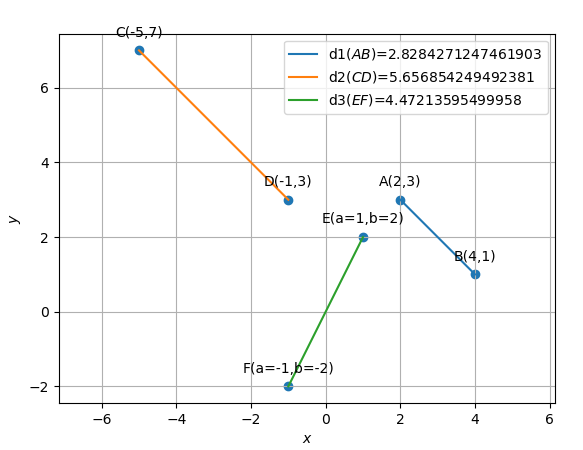
\includegraphics[width=\columnwidth]{chapters/10/7/1/1/figs/graph.png}
	\end{center}
\caption{}
\label{fig:10/7/1/1Fig}
\end{figure}
\end{enumerate}

\item Find the distance between the points $(0,0)$ and $ (36,15)$.
	\\
		\solution
		\iffalse
\documentclass[journal,12pt,twocolumn]{IEEEtran}
\usepackage{graphicx}
\graphicspath{{./chapters/10/7/1/2/figs/}}{}
\usepackage{amsmath,amssymb,amsfonts,amsthm}
\newcommand{\myvec}[1]{\ensuremath{\begin{pmatrix}#1\end{pmatrix}}}
\providecommand{\norm}[1]{\lVert#1\rVert}
\usepackage{listings}
\usepackage{watermark}
\usepackage{titlesec}
\usepackage{caption}
\let\vec\mathbf
\lstset{
frame=single, 
breaklines=true,
columns=fullflexible
}
\thiswatermark{\centering \put(0,-105.0){
\includegraphics[scale=0.15]{/sdcard/IITH/vector/chapters/10/7/1/2/figs/logo2.png}} }
\title{\mytitle}
\title{
Assignment - Vector
}
\author{Surajit Sarkar}
\begin{document}
\maketitle
\tableofcontents
\bigskip
\section{\textbf{Problem}}
Find the distance between the point(0,0) and (36,15).Can you now find the distance between the two towns A and B discussed in Section 7.2
\section{\textbf{Solution}}
\fi
Let
\begin{align}
\vec{A}&=\myvec{0 \\ 0}  
\Vec{B}=\myvec{36 \\ 15} \\ 
\implies 
\vec{d}&=\norm{\vec{A}-\vec{B}}=\sqrt{\myvec{\vec{A}-\vec{B}}^T\myvec{\vec{A}-\vec{B}}} \\
&=39
\end{align}
See Fig. 
\ref{fig:10/7/1/2vec}.
\begin{figure}[!h]
\centering
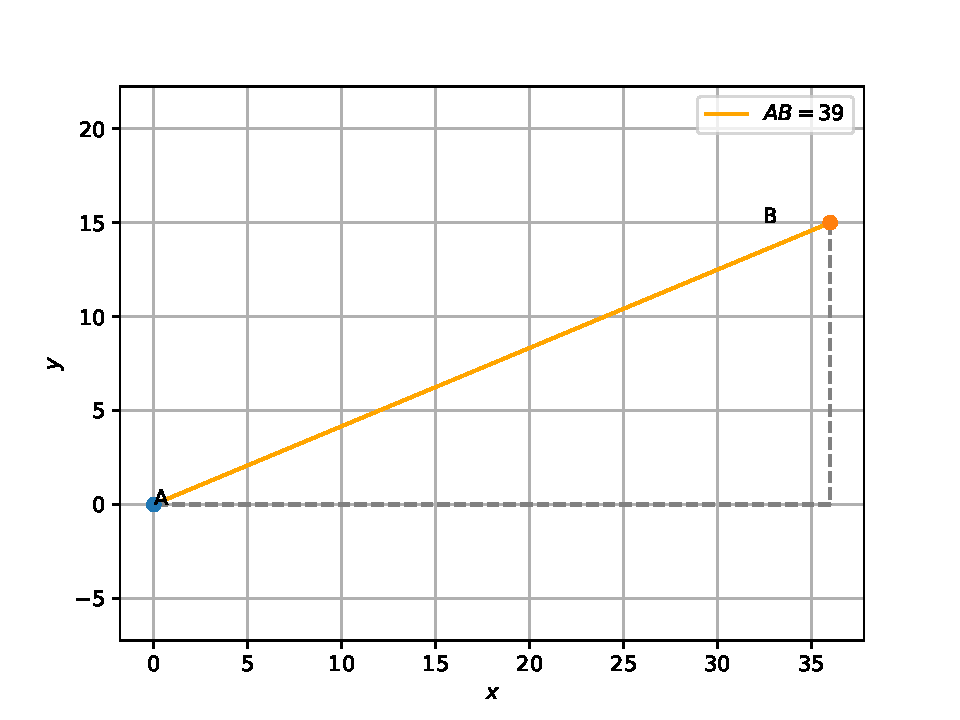
\includegraphics[width=\columnwidth]{chapters/10/7/1/2/figs/vec.pdf}
\caption{}
\label{fig:10/7/1/2vec}
\end{figure}

\item Determine if the points $(1,5),(2,3)$ and $(-2,-11)$ are collinear.
	\\
		\iffalse
\documentclass[12pt]{article}
\usepackage{graphicx}
\usepackage[none]{hyphenat}
\usepackage{graphicx}
\usepackage{listings}
\usepackage[english]{babel}
\usepackage{graphicx}
\usepackage{caption} 
\usepackage{hyperref}
\usepackage{booktabs}
\usepackage{array}
\usepackage{amsmath}   % for having text in math mode
\usepackage{extarrows} % for Row operations arrows
\usepackage{listings}
\lstset{
  frame=single,
  breaklines=true
}
  
%Following 2 lines were added to remove the blank page at the beginning
\usepackage{atbegshi}% http://ctan.org/pkg/atbegshi
\AtBeginDocument{\AtBeginShipoutNext{\AtBeginShipoutDiscard}}


%New macro definitions
\newcommand{\mydet}[1]{\ensuremath{\begin{vmatrix}#1\end{vmatrix}}}
\providecommand{\brak}[1]{\ensuremath{\left(#1\right)}}
\providecommand{\norm}[1]{\left\lVert#1\right\rVert}
\newcommand{\solution}{\noindent \textbf{Solution: }}
\newcommand{\myvec}[1]{\ensuremath{\begin{pmatrix}#1\end{pmatrix}}}
\let\vec\mathbf

\begin{document}

\begin{center}
\title{\textbf{Properties of Triangles}}
\date{\vspace{-5ex}} %Not to print date automatically
\maketitle
\end{center}
\setcounter{page}{1}

\section{10$^{th}$ Maths - Chapter 7}
This is Problem-3 from Exercise 7.1
\begin{enumerate}
\item Determine if the points $(1,5), (2,3), \text{ and } (-2,-11)$ are collinear.  \\
	\fi
\solution 
 We know that points $\vec{A}, \vec{B} \text{ and } \vec{C}$ are collinear, if
\begin{align}
  \label{eq:10/7/1/31}
\text{rank}\myvec{ 
	\vec{A}^\top \\ 
	\vec{B}^\top \\ 
	\vec{C}^\top 
}    &=  1 
\end{align}
Since
\begin{align}
	\myvec{ \vec{A}^\top \\ 
			\vec{B}^\top \\ 
			\vec{C}^\top 
} =   		\myvec{
        		1 & 5 \\
        		2 & 3 \\
        		-2 & -11 
}
\\
\xleftrightarrow[{R_3\rightarrow R_3+2R_1}]{{R_2\rightarrow R_2-2R_1}}  \myvec{
  1 & 5 \\
  0 & -7 \\
  0 & -1 
}    
\xleftrightarrow[]{{R_3\rightarrow R_3-\frac{1}{7}R_2}}  \myvec{
  1 & 5 \\
  0 & -7 \\
  0 & 0 
},
\end{align}
 the rank of the matrix is 2. From \eqref{eq:10/7/1/31}, the points are not collinear.  This is verified by Fig.  
 \ref{fig:10/7/1/3Fig1}, where the given points constitute a triangle and not a line.
\begin{figure}[!h]
	\begin{center}
		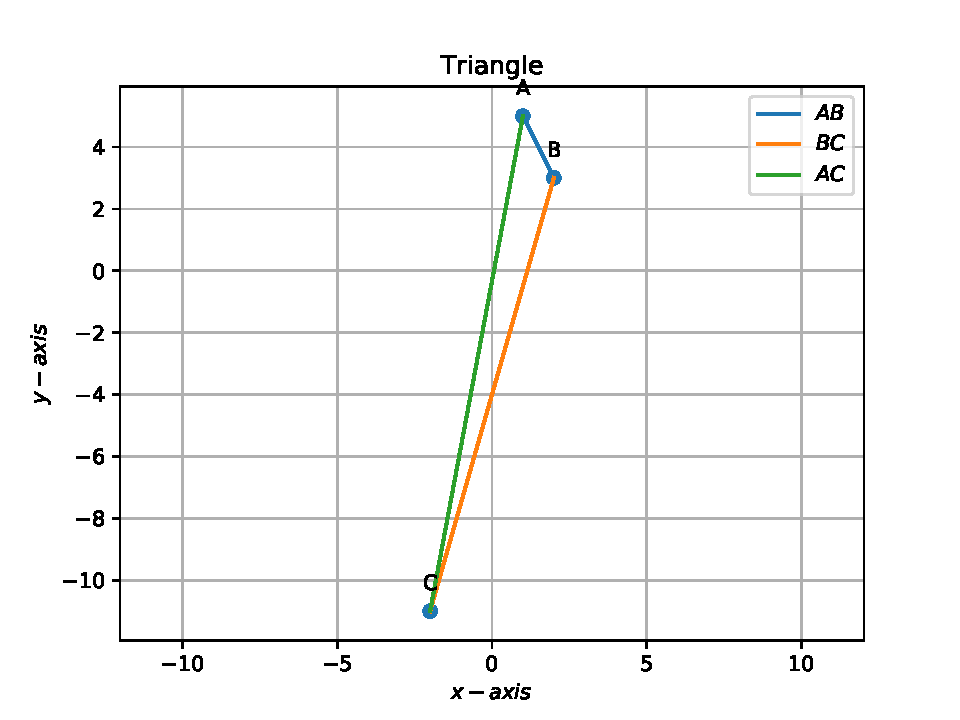
\includegraphics[width=\columnwidth]{chapters/10/7/1/3/figs/problem3.pdf}
	\end{center}
\caption{}
\label{fig:10/7/1/3Fig1}
\end{figure}


\item Check whether$(5,-2),(6,4)$ and $(7,-2)$ are the vertices of an isosceles triangle.
	\iffalse
\item  In a classroom, 4 friends are seated at the points A,B,C and D as shown in Fig. 7.8, Champa and Chameli walk in to the class and after observing for a few minutes Champa asks Chameli,"Dont't you think ABCD is a square?" Chameli disagrees,Using distance formula, find which of them is correct.

\begin{figure}[!h]
\centering
  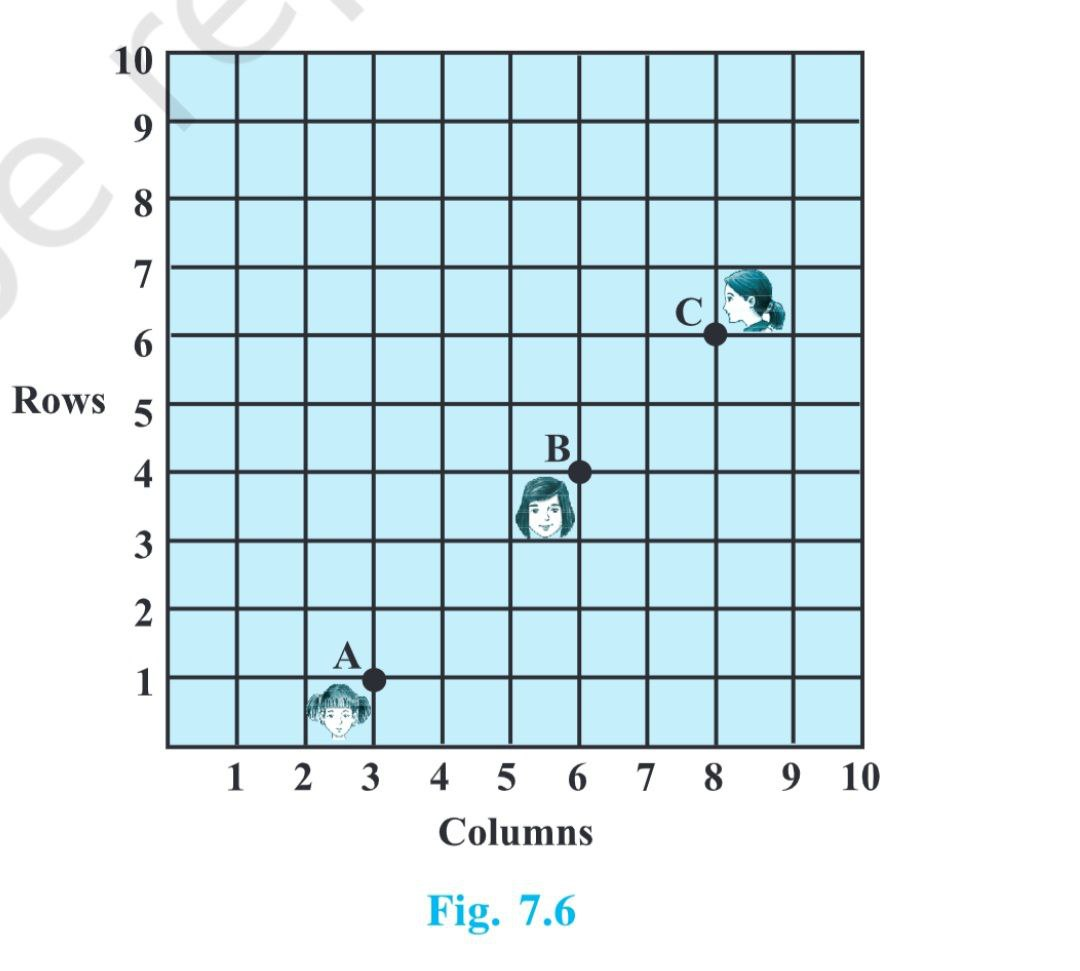
\includegraphics[width=\columnwidth]{canvas.jpg}
 \caption{}
\label{fig:10/7/4/8Fig3}
\end{figure}
\fi
\item Name the type of quadrilateral formed,if any,by the following points,and give reasons for your answer
\begin{enumerate}
\item $(-1,-2),(1,0),(-1,2),(-3,0)$
\item $(-3,5),(-3,1),(0,3),(-1,-4)$
\item $(4,5),(7,6),(4,3),(1,2)$
\end{enumerate}
\solution
		\iffalse
\documentclass[12pt]{article}
\usepackage{graphicx}
\usepackage{amsmath}
\usepackage{mathtools}
\usepackage{gensymb}

\newcommand{\mydet}[1]{\ensuremath{\begin{vmatrix}#1\end{vmatrix}}}
\providecommand{\brak}[1]{\ensuremath{\left(#1\right)}}
\providecommand{\norm}[1]{\left\lVert#1\right\rVert}
\newcommand{\solution}{\noindent \textbf{Solution: }}
\newcommand{\myvec}[1]{\ensuremath{\begin{pmatrix}#1\end{pmatrix}}}
\let\vec\mathbf

\begin{document}
\begin{center}
\textbf\large{CHAPTER-7 \\ COORDINATE GEOMETRY}

\end{center}
\section*{Excercise 7.1}

Q6.Name the type of quadilateral formed,if any, by the following points, and give reasons for your answer:
\begin{enumerate}
	\item $\brak{-1,-2}, \brak{1,0}, \brak{-1,2}, \brak{-3,0}$ 
	\item $\brak{-3,5}, \brak{3,1}, \brak{0,3}, \brak{-1,-4}$
	\item $\brak{4,5}, \brak{7,6}, \brak{4,3}, \brak{1,2}$
\end{enumerate}
\solution
\fi
\begin{enumerate}
\item The coordinates are given as
	\begin{align}
	\vec{A} = \myvec{
		-1\\
		-2\\
		},
	\vec{B} = \myvec{
		1\\
		0\\
		},
	\vec{C} = \myvec{
		-1\\
		2\\
		} \text{ and }
	\vec{D} = \myvec{
		-3\\
		0\\
		}
	\end{align}
	\begin{align}
		\vec{B} - \vec{A} &= \myvec{1\\0} - \myvec{-1\\-2} = \myvec{2\\2}\\
		\vec{C} - \vec{B} &= \myvec{-1\\2} - \myvec{1\\0} = \myvec{-2\\2}\\
		\vec{C} - \vec{D} &= \myvec{-1\\2} - \myvec{-3\\0} = \myvec{2\\2}\\
		\vec{D} - \vec{A} &= \myvec{-3\\0} - \myvec{-1\\-2} = \myvec{-2\\2}
	\end{align}
	\begin{align}	
		\vec{C} - \vec{A} &= \myvec{-1\\2} - \myvec{-1\\-2} = \myvec{0\\4}\\
		\vec{D} - \vec{B} &= \myvec{-3\\0} - \myvec{1\\0} = \myvec{-4\\0}
	\end{align}
	\begin{align}	
		\vec{B}-\vec{A} = \vec{C}-\vec{D} \text{ and } \vec{C}-\vec{B} = \vec{D}-\vec{A}.
	\end{align}
	Hence, $ABCD$ is a parallelogram.
	\begin{enumerate}
		\item Now checking if the adjacent sides are orthogonal to each other
	\begin{align}
		(\vec{B}-\vec{A})^\top (\vec{C}-\vec{B}) = \myvec{2&2} \myvec{-2\\2} = -4+4 = 0
	\end{align}
		\item Now checking if the diagonals are also orthogonal then it is a square else a rectangle.
	\end{enumerate}	
	\begin{align}
		(\vec{C}-\vec{A})^\top (\vec{D}-\vec{B}) = \myvec{0&4} \myvec{-4\\0} = 0
	\end{align}
	Hence the diagonals are orthogonal to each other.

	So, we can conclude that $ABCD$ is a square.

	As shown in Figure \ref{fig:10/7/1/6/Fig1} we can see that $ABCD$ is a square hence we can conclude that our theoritical result is verified.
 
\begin{figure}[!h]
	\begin{center} 
	    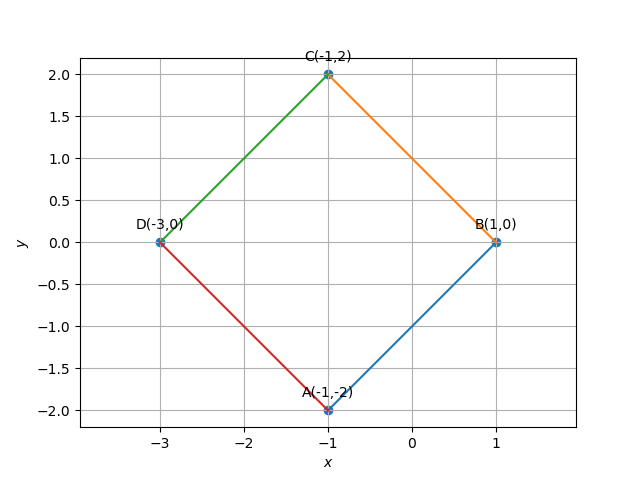
\includegraphics[width=\columnwidth]{chapters/10/7/1/6/figs/quad1}
	\end{center}
\caption{}
\label{fig:10/7/1/6/Fig1}
\end{figure}

\item The coordinates are given as
	\begin{align}
	\vec{A} = \myvec{
		-3\\
		5\\
		},
	\vec{B} = \myvec{
		3\\
		1\\
		},
	\vec{C} = \myvec{
		0\\
		3\\
		} \text{ and }
	\vec{D} = \myvec{
		-1\\
		-4\\
		}
	\end{align}
	\begin{align}
		\vec{B} - \vec{A} &= \myvec{3\\1} - \myvec{-3\\5} = \myvec{6\\-4}\\
		\vec{C} - \vec{B} &= \myvec{0\\3} - \myvec{3\\1} = \myvec{-3\\2}\\
		\vec{C} - \vec{D} &= \myvec{0\\3} - \myvec{-1\\-4} = \myvec{1\\7}\\
		\vec{D} - \vec{A} &= \myvec{-1\\-4} - \myvec{-3\\5} = \myvec{2\\-9}
	\end{align}
	\begin{align}
		\vec{C} - \vec{A} &= \myvec{0\\3} - \myvec{-3\\5} = \myvec{3\\-2}\\
		\vec{D} - \vec{B} &= \myvec{-1\\-4} - \myvec{3\\1} = \myvec{-4\\-5}
	\end{align}
	\begin{align}
	\vec{B}-\vec{A} \neq \vec{C}-\vec{D} \text{ and } \vec{C}-\vec{B} \neq \vec{D}-\vec{A},
	\end{align}
	Hence, $ABCD$ is not a parallelogram, it can be a irregular quadilateral.
	\begin{enumerate}
		\item Now to check if any three points are collinear,

	if rank of $\myvec{\vec{B}-\vec{A} & \vec{C}-\vec{B}} = 1$ then points are collinear

	Forming the collinearity matrix
	\begin{align}
		\myvec{6&-3\\-4&2} \xleftrightarrow{R_{2}\rightarrow R_{2}+\frac{2}{3}R_{1}}= \myvec{6&-3\\0&0}
	\end{align}
	\end{enumerate}
	Hence, rank = 1

	Since none of the opposite sides are parallel to each other and three points are collinear so these does not form a quadilateral.

	As shown in Figure \ref{fig:10/7/1/6/Fig2} we can see that $ABCD$ does not form a quadilateral and three points are collinear hence, our theoritical result is verified.
	
\begin{figure}[!h]
	\begin{center} 
	    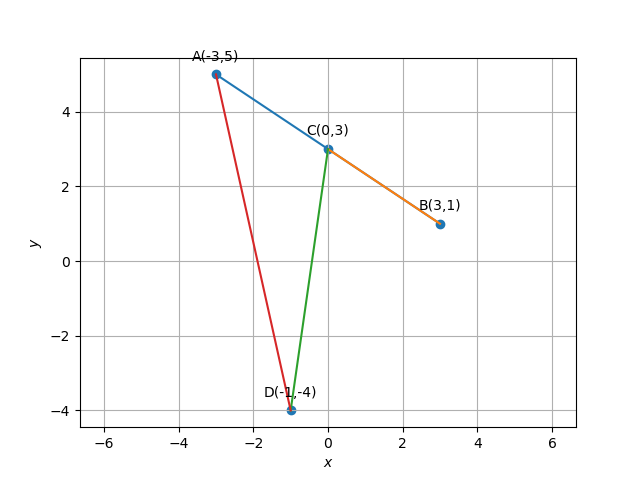
\includegraphics[width=\columnwidth]{chapters/10/7/1/6/figs/quad2}
	\end{center}
\caption{}
\label{fig:10/7/1/6/Fig2}
\end{figure}
	
\item The coordinates are given as
	\begin{align}
	\vec{A} = \myvec{
		4\\
		5\\
		},
	\vec{B} = \myvec{
		7\\
		6\\
		},
	\vec{C} = \myvec{
		4\\
		3\\
		} \text{ and }
	\vec{D} = \myvec{
		1\\
		2\\
		}
	\end{align}
	\begin{align}
		\vec{B} - \vec{A} &= \myvec{7\\6} - \myvec{4\\5} = \myvec{3\\1}\\
		\vec{C} - \vec{B} &= \myvec{4\\3} - \myvec{7\\6} = \myvec{-3\\-3}\\
		\vec{C} - \vec{D} &= \myvec{4\\3} - \myvec{1\\2} = \myvec{3\\1}\\
		\vec{D} - \vec{A} &= \myvec{1\\2} - \myvec{4\\5} = \myvec{-3\\-3}
	\end{align}
	\begin{align}
		\vec{C} - \vec{A} &= \myvec{4\\3} - \myvec{4\\5} = \myvec{0\\-2}\\
		\vec{D} - \vec{B} &= \myvec{1\\2} - \myvec{7\\6} = \myvec{-6\\-4}
	\end{align}
	\begin{align}
		\vec{B}-\vec{A} = \vec{C}-\vec{D} \text{ and } \vec{C}-\vec{B} = \vec{D}-\vec{A},
	\end{align}
	Hence, $ABCD$ is a parallelogram.
	\begin{enumerate}
		\item Now checking if the adjacent sides are orthogonal to each other
	\begin{align}
		(\vec{B}-\vec{A})^\top (\vec{C}-\vec{B}) = \myvec{3&1} \myvec{-3\\-3} = -9-3 = -12
	\end{align}
	Since inner product is not zero so adjacent sides are not orthogonal.

	Hence, we can say that $ABCD$ is neither a rectangle nor a square.

		\item Now checking if the diagonals are orthogonal then it is a Rhombus.
	\begin{align}
		(\vec{C}- \vec{A})^\top (\vec{D}-\vec{B}) = \myvec{0&-2} \myvec{-6\\-4} = 0+8 = 8
	\end{align}
	\end{enumerate}		
	Hence the diagonals are also not orthogonal so we conclude that $ABCD$ is a parallelogram.

	As shown in Figure \ref{fig:10/7/1/6/Fig3} we can see that $ABCD$ forms a parallelogram hence, our theoritical result is verified.

\begin{figure}[!h]
	\begin{center} 
	    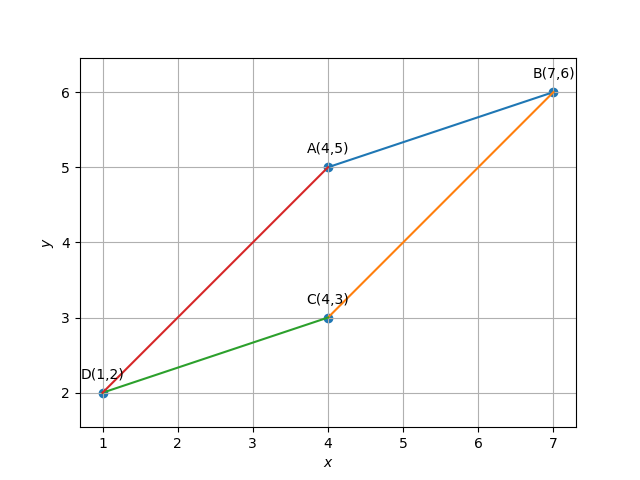
\includegraphics[width=\columnwidth]{chapters/10/7/1/6/figs/quad3}
	\end{center}
\caption{}
\label{fig:10/7/1/6/Fig3}
\end{figure}
\end{enumerate}



\item Find the point on the x-axis which is equidistant from $(2,-5)$ and $(-2,9)$.
	\\
\solution
		\iffalse
\documentclass[12pt]{article}
\usepackage{graphicx}
%\documentclass[journal,12pt,twocolumn]{IEEEtran}
\usepackage[none]{hyphenat}
\usepackage{graphicx}
\usepackage{listings}
\usepackage[english]{babel}
\usepackage{graphicx}
\usepackage{caption} 
\usepackage{hyperref}
\usepackage{booktabs}
\def\inputGnumericTable{}
\usepackage{color}                                            %%
    \usepackage{array}                                            %%
    \usepackage{longtable}                                        %%
    \usepackage{calc}                                             %%
    \usepackage{multirow}                                         %%
    \usepackage{hhline}                                           %%
    \usepackage{ifthen}
\usepackage{array}
\usepackage{amsmath}   % for having text in math mode
\usepackage{listings}
\lstset{
language=tex,
frame=single, 
breaklines=true
}
  
%Following 2 lines were added to remove the blank page at the beginning
\usepackage{atbegshi}% http://ctan.org/pkg/atbegshi
\AtBeginDocument{\AtBeginShipoutNext{\AtBeginShipoutDiscard}}
%


%New macro definitions
\newcommand{\mydet}[1]{\ensuremath{\begin{vmatrix}#1\end{vmatrix}}}
\providecommand{\brak}[1]{\ensuremath{\left(#1\right)}}
\providecommand{\norm}[1]{\left\lVert#1\right\rVert}
\newcommand{\solution}{\noindent \textbf{Solution: }}
\newcommand{\myvec}[1]{\ensuremath{\begin{pmatrix}#1\end{pmatrix}}}
\let\vec\mathbf

\begin{document}

\begin{center}
\title{\textbf{Coordinate Geometry}}
\date{\vspace{-5ex}} %Not to print date automatically
\maketitle
\end{center}

\setcounter{page}{1}



\section*{10$^{th}$ Maths - Chapter 7}

This is Problem-7 from Exercise 7.1

\begin{enumerate}

\item The point on the $x$-axis which is equidistant from $\myvec{2 \\ -5}$ and $\myvec{-2\\9}$\\
\solution \\
\fi
		The input parameters for this problem are available in Table \ref{tab:10/7/1/7Table-1}
\begin{table}[ht!]
%%%%%%%%%%%%%%%%%%%%%%%%%%%%%%%%%%%%%%%%%%%%%%%%%%%%%%%%%%%%%%%%%%%%%%
%%                                                                  %%
%%  This is the header of a LaTeX2e file exported from Gnumeric.    %%
%%                                                                  %%
%%  This file can be compiled as it stands or included in another   %%
%%  LaTeX document. The table is based on the longtable package so  %%
%%  the longtable options (headers, footers...) can be set in the   %%
%%  preamble section below (see PRAMBLE).                           %%
%%                                                                  %%
%%  To include the file in another, the following two lines must be %%
%%  in the including file:                                          %%
%%        \def\inputGnumericTable{}                                 %%
%%  at the beginning of the file and:                               %%
%%        \input{name-of-this-file.tex}                             %%
%%  where the table is to be placed. Note also that the including   %%
%%  file must use the following packages for the table to be        %%
%%  rendered correctly:                                             %%
%%    \usepackage[latin1]{inputenc}                                 %%
%%    \usepackage{color}                                            %%
%%    \usepackage{array}                                            %%
%%    \usepackage{longtable}                                        %%
%%    \usepackage{calc}                                             %%
%%    \usepackage{multirow}                                         %%
%%    \usepackage{hhline}                                           %%
%%    \usepackage{ifthen}                                           %%
%%  optionally (for landscape tables embedded in another document): %%
%%    \usepackage{lscape}                                           %%
%%                                                                  %%
%%%%%%%%%%%%%%%%%%%%%%%%%%%%%%%%%%%%%%%%%%%%%%%%%%%%%%%%%%%%%%%%%%%%%%



%%  This section checks if we are begin input into another file or  %%
%%  the file will be compiled alone. First use a macro taken from   %%
%%  the TeXbook ex 7.7 (suggestion of Han-Wen Nienhuys).            %%
\def\ifundefined#1{\expandafter\ifx\csname#1\endcsname\relax}


%%  Check for the \def token for inputed files. If it is not        %%
%%  defined, the file will be processed as a standalone and the     %%
%%  preamble will be used.                                          %%
\ifundefined{inputGnumericTable}

%%  We must be able to close or not the document at the end.        %%
	\def\gnumericTableEnd{\end{document}}


%%%%%%%%%%%%%%%%%%%%%%%%%%%%%%%%%%%%%%%%%%%%%%%%%%%%%%%%%%%%%%%%%%%%%%
%%                                                                  %%
%%  This is the PREAMBLE. Change these values to get the right      %%
%%  paper size and other niceties.                                  %%
%%                                                                  %%
%%%%%%%%%%%%%%%%%%%%%%%%%%%%%%%%%%%%%%%%%%%%%%%%%%%%%%%%%%%%%%%%%%%%%%

	\documentclass[12pt%
			  %,landscape%
                    ]{report}
       \usepackage[latin1]{inputenc}
       \usepackage{fullpage}
       \usepackage{color}
       \usepackage{array}
       \usepackage{longtable}
       \usepackage{calc}
       \usepackage{multirow}
       \usepackage{hhline}
       \usepackage{ifthen}

	\begin{document}


%%  End of the preamble for the standalone. The next section is for %%
%%  documents which are included into other LaTeX2e files.          %%
\else

%%  We are not a stand alone document. For a regular table, we will %%
%%  have no preamble and only define the closing to mean nothing.   %%
    \def\gnumericTableEnd{}

%%  If we want landscape mode in an embedded document, comment out  %%
%%  the line above and uncomment the two below. The table will      %%
%%  begin on a new page and run in landscape mode.                  %%
%       \def\gnumericTableEnd{\end{landscape}}
%       \begin{landscape}


%%  End of the else clause for this file being \input.              %%
\fi

%%%%%%%%%%%%%%%%%%%%%%%%%%%%%%%%%%%%%%%%%%%%%%%%%%%%%%%%%%%%%%%%%%%%%%
%%                                                                  %%
%%  The rest is the gnumeric table, except for the closing          %%
%%  statement. Changes below will alter the table's appearance.     %%
%%                                                                  %%
%%%%%%%%%%%%%%%%%%%%%%%%%%%%%%%%%%%%%%%%%%%%%%%%%%%%%%%%%%%%%%%%%%%%%%

\providecommand{\gnumericmathit}[1]{#1} 
%%  Uncomment the next line if you would like your numbers to be in %%
%%  italics if they are italizised in the gnumeric table.           %%
%\renewcommand{\gnumericmathit}[1]{\mathit{#1}}
\providecommand{\gnumericPB}[1]%
{\let\gnumericTemp=\\#1\let\\=\gnumericTemp\hspace{0pt}}
 \ifundefined{gnumericTableWidthDefined}
        \newlength{\gnumericTableWidth}
        \newlength{\gnumericTableWidthComplete}
        \newlength{\gnumericMultiRowLength}
        \global\def\gnumericTableWidthDefined{}
 \fi
%% The following setting protects this code from babel shorthands.  %%
 \ifthenelse{\isundefined{\languageshorthands}}{}{\languageshorthands{english}}
%%  The default table format retains the relative column widths of  %%
%%  gnumeric. They can easily be changed to c, r or l. In that case %%
%%  you may want to comment out the next line and uncomment the one %%
%%  thereafter                                                      %%
\providecommand\gnumbox{\makebox[0pt]}
%%\providecommand\gnumbox[1][]{\makebox}

%% to adjust positions in multirow situations                       %%
\setlength{\bigstrutjot}{\jot}
\setlength{\extrarowheight}{\doublerulesep}

%%  The \setlongtables command keeps column widths the same across  %%
%%  pages. Simply comment out next line for varying column widths.  %%
\setlongtables

\setlength\gnumericTableWidth{%
	53pt+%
	53pt+%
	82pt+%
	53pt+%
0pt}
\def\gumericNumCols{4}
\setlength\gnumericTableWidthComplete{\gnumericTableWidth+%
         \tabcolsep*\gumericNumCols*2+\arrayrulewidth*\gumericNumCols}
\ifthenelse{\lengthtest{\gnumericTableWidthComplete > \linewidth}}%
         {\def\gnumericScale{1*\ratio{\linewidth-%
                        \tabcolsep*\gumericNumCols*2-%
                        \arrayrulewidth*\gumericNumCols}%
{\gnumericTableWidth}}}%
{\def\gnumericScale{1}}

%%%%%%%%%%%%%%%%%%%%%%%%%%%%%%%%%%%%%%%%%%%%%%%%%%%%%%%%%%%%%%%%%%%%%%
%%                                                                  %%
%% The following are the widths of the various columns. We are      %%
%% defining them here because then they are easier to change.       %%
%% Depending on the cell formats we may use them more than once.    %%
%%                                                                  %%
%%%%%%%%%%%%%%%%%%%%%%%%%%%%%%%%%%%%%%%%%%%%%%%%%%%%%%%%%%%%%%%%%%%%%%

\ifthenelse{\isundefined{\gnumericColA}}{\newlength{\gnumericColA}}{}\settowidth{\gnumericColA}{\begin{tabular}{@{}p{53pt*\gnumericScale}@{}}x\end{tabular}}
\ifthenelse{\isundefined{\gnumericColB}}{\newlength{\gnumericColB}}{}\settowidth{\gnumericColB}{\begin{tabular}{@{}p{53pt*\gnumericScale}@{}}x\end{tabular}}
\ifthenelse{\isundefined{\gnumericColC}}{\newlength{\gnumericColC}}{}\settowidth{\gnumericColC}{\begin{tabular}{@{}p{82pt*\gnumericScale}@{}}x\end{tabular}}
\ifthenelse{\isundefined{\gnumericColD}}{\newlength{\gnumericColD}}{}\settowidth{\gnumericColD}{\begin{tabular}{@{}p{53pt*\gnumericScale}@{}}x\end{tabular}}

	\begin{center}
\begin{tabular}[c]{%
	b{\gnumericColA}%
	b{\gnumericColB}%
	b{\gnumericColC}%
	b{\gnumericColD}%
	}

%%%%%%%%%%%%%%%%%%%%%%%%%%%%%%%%%%%%%%%%%%%%%%%%%%%%%%%%%%%%%%%%%%%%%%
%%  The longtable options. (Caption, headers... see Goosens, p.124) %%
%	\caption{The Table Caption.}             \\	%
% \hline	% Across the top of the table.
%%  The rest of these options are table rows which are placed on    %%
%%  the first, last or every page. Use \multicolumn if you want.    %%

%%  Header for the first page.                                      %%
%	\multicolumn{4}{c}{The First Header} \\ \hline 
%	\multicolumn{1}{c}{colTag}	%Column 1
%	&\multicolumn{1}{c}{colTag}	%Column 2
%	&\multicolumn{1}{c}{colTag}	%Column 3
%	&\multicolumn{1}{c}{colTag}	\\ \hline %Last column
%	\endfirsthead

%%  The running header definition.                                  %%
%	\hline
%	\multicolumn{4}{l}{\ldots\small\slshape continued} \\ \hline
%	\multicolumn{1}{c}{colTag}	%Column 1
%	&\multicolumn{1}{c}{colTag}	%Column 2
%	&\multicolumn{1}{c}{colTag}	%Column 3
%	&\multicolumn{1}{c}{colTag}	\\ \hline %Last column
%	\endhead

%%  The running footer definition.                                  %%
%	\hline
%	\multicolumn{4}{r}{\small\slshape continued\ldots} \\
%	\endfoot

%%  The ending footer definition.                                   %%
%	\multicolumn{4}{c}{That's all folks} \\ \hline 
%	\endlastfoot
%%%%%%%%%%%%%%%%%%%%%%%%%%%%%%%%%%%%%%%%%%%%%%%%%%%%%%%%%%%%%%%%%%%%%%

\hhline{|-|-|-~}
	 \multicolumn{1}{|p{\gnumericColA}|}%
	{\gnumericPB{\centering}\gnumbox{\textbf{Symbol}}}
	&\multicolumn{1}{p{\gnumericColB}|}%
	{\gnumericPB{\centering}\gnumbox{\textbf{Value}}}
	&\multicolumn{1}{p{\gnumericColC}|}%
	{\gnumericPB{\centering}\gnumbox{\textbf{Description}}}
	&
\\
\hhline{|---|~}
	 \multicolumn{1}{|p{\gnumericColA}|}%
	{\gnumericPB{\centering}\gnumbox{$\vec{A}$}}
	&\multicolumn{1}{p{\gnumericColB}|}%
	{\gnumericPB{\centering}\gnumbox{$\myvec{2\\-5}$}}
	&\multicolumn{1}{p{\gnumericColC}|}%
	{\gnumericPB{\centering}\gnumbox{First point}}
	&
\\
\hhline{|---|~}
	 \multicolumn{1}{|p{\gnumericColA}|}%
	{\gnumericPB{\centering}\gnumbox{$\vec{B}$}}
	&\multicolumn{1}{p{\gnumericColB}|}%
	{\gnumericPB{\centering}\gnumbox{$\myvec{-2\\9}$}}
	&\multicolumn{1}{p{\gnumericColC}|}%
	{\gnumericPB{\centering}\gnumbox{Second point}}
	&
\\
\hhline{|---|~}
	 \multicolumn{1}{|p{\gnumericColA}|}%
	{\gnumericPB{\centering}\gnumbox{$\vec{O}$}}
	&\multicolumn{1}{p{\gnumericColB}|}%
	{\gnumericPB{\centering}\gnumbox{$?$}}
	&\multicolumn{1}{p{\gnumericColC}|}%
	{\gnumericPB{\centering}\gnumbox{Desired point}}
	&
\\
\hhline{|-|-|-|~}
\end{tabular}
	\end{center}

\ifthenelse{\isundefined{\languageshorthands}}{}{\languageshorthands{\languagename}}
\gnumericTableEnd

\caption{}
\label{tab:10/7/1/7Table-1}	
\end{table}
%
  If $\vec{O}$ lies on the  $x$-axis and is  equidistant from the points $\vec{A}$ and $\vec{B}$, 
\begin{align}
 \norm{\vec{O}-\vec{A}} &=
\norm{\vec{A}-\vec{B}} 
\\
 \implies \norm{\vec{O}-\vec{A}}^2 &=
\norm{\vec{O}-\vec{B}}^2 
\end{align}
which can be expressed as 
\begin{multline}
%  \label{eq:10/7/1/7norm2d_dist}
 \brak{\vec{O}-\vec{A}}^{\top} \brak{\vec{O}-\vec{A}}=
 \brak{\vec{O}-\vec{B}}^{\top} 
\brak{\vec{O}-\vec{B}}
\\
 \implies \norm{\vec{O}}^2-2{\vec{O}}^{\top}\vec{A} + \norm{\vec{A}}^2
 \\= \norm{\vec{O}}^2-2{\vec{O}}^{\top}\vec{B} + \norm{\vec{B}}^2
\end{multline}
which can be simplified to obtain
%  \eqref{eq:10/7/1/7norm2d_equidist}.
  \begin{align}
   \vec{O} &=
    x\vec{e}_1
  \end{align}
  where 
  \begin{align}
   x &=\frac{\norm{\vec{A}}^2 -\norm{\vec{B}}^2 }{2\brak{\vec{A}-\vec{B}}^{\top }\vec{e}_1
}\label{eq:10/7/1/75}  
  \end{align}
  Substituting from Table \eqref{tab:10/7/1/7Table-1} in \eqref{eq:10/7/1/75},
\begin{align}
 \brak{\vec{A}-\vec{B}}^{\top}=
 \brak{\myvec{2 \\ -5}-\myvec{-2\\9}}^{\top}
	&=\myvec{4 & -14}
	\\
	\norm{\vec{A}}^2 = 21,
	\norm{\vec{B}}^2 &= 85
    \end{align}
yielding $x$ = $ -7$.  Thus, 
		\begin{align}
\vec{O} = \myvec{ -7 \\ 0}.
		\end{align}
		See Fig. 
\ref{fig:10/7/1/7Fig1}.

\begin{figure}[!h]
 \begin{center}
  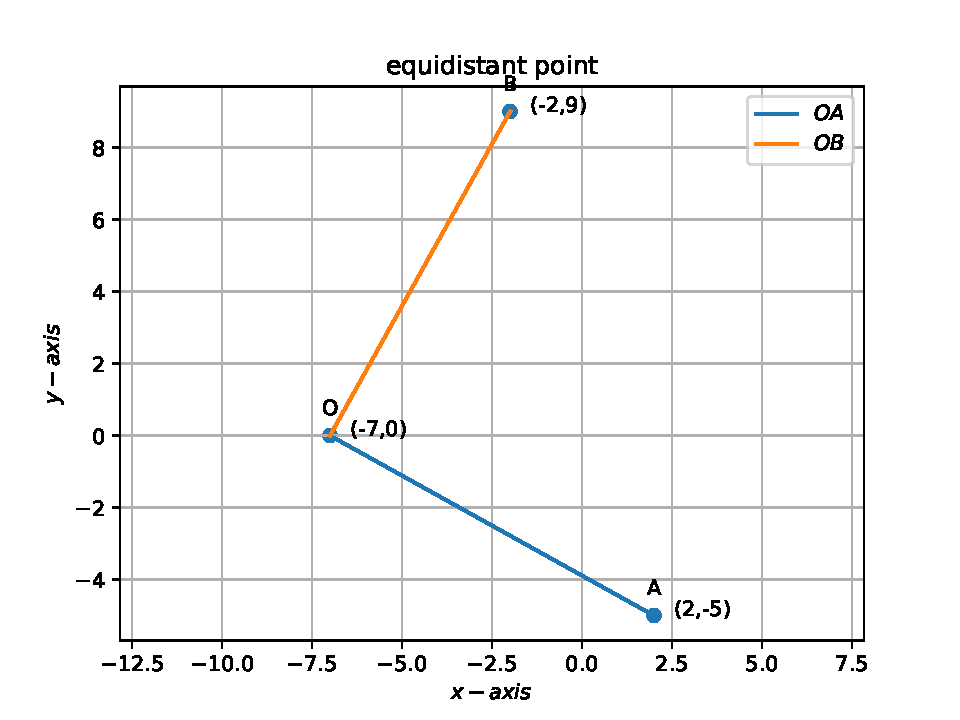
\includegraphics[width=\columnwidth]{chapters/10/7/1/7/figs/fig.pdf}
 \end{center}
\caption{}
\label{fig:10/7/1/7Fig1}
\end{figure}


\item Find the values of $y$ for which the distance between the points                  $\vec{P}(2,-3)$ and $\vec{Q}(10,y)$ is 10 units.
\item  If $\vec{Q}(0, 1)$ is equidistant from $\vec{P}(5, -3)$ and $\vec{R}(x, 6)$, find the values of $x$. Also find the
distances $QR$ and $PR$.
\item  Find a relation between $x$ and $y$ such that the point $(x,y)$ is equidistant from the point
$(3, 6)$ and $(– 3, 4)$.
	\\
\solution
		\iffalse
\documentclass[12pt]{article}
\usepackage{graphicx}
%\documentclass[journal,12pt,twocolumn]{IEEEtran}
\usepackage[none]{hyphenat}
\usepackage{graphicx}
\usepackage{listings}
\usepackage[english]{babel}
\usepackage{graphicx}
\usepackage{caption} 
\usepackage{hyperref}
\usepackage{booktabs}
\def\inputGnumericTable{}
\usepackage{color}                                            %%
    \usepackage{array}                                            %%
    \usepackage{longtable}                                        %%
    \usepackage{calc}                                             %%
    \usepackage{multirow}                                         %%
    \usepackage{hhline}                                           %%
    \usepackage{ifthen}
\usepackage{array}
\usepackage{amsmath}   % for having text in math mode
\usepackage{listings}
\lstset{
language=tex,
frame=single, 
breaklines=true
}
  
%Following 2 lines were added to remove the blank page at the beginning
\usepackage{atbegshi}% http://ctan.org/pkg/atbegshi
\AtBeginDocument{\AtBeginShipoutNext{\AtBeginShipoutDiscard}}
%


%New macro definitions
\newcommand{\mydet}[1]{\ensuremath{\begin{vmatrix}#1\end{vmatrix}}}
\providecommand{\brak}[1]{\ensuremath{\left(#1\right)}}
\providecommand{\norm}[1]{\left\lVert#1\right\rVert}
\newcommand{\solution}{\noindent \textbf{Solution: }}
\newcommand{\myvec}[1]{\ensuremath{\begin{pmatrix}#1\end{pmatrix}}}
\let\vec\mathbf

\begin{document}

\begin{center}
\title{\textbf{Coordinate Geometry}}
\date{\vspace{-5ex}} %Not to print date automatically
\maketitle
\end{center}

\setcounter{page}{1}



\begin{enumerate}

\item\textbf{Problem statement :} Find a relation between x and y such that the point $\myvec{x ,y}$ is equidistant from the point $\myvec{3 ,6}$ and $\myvec{-3 ,4}$

\solution \\
\textbf{\centering{Method I}}
\fi
The input parameters for this problem are given as
	\begin{align}
	\vec{P} = \myvec{
		x\\
		y\\
		},
	\vec{A} = \myvec{
		3\\
		6\\
		},
        \vec{B} = \myvec{
		3\\
		-4\\
		}
	\end{align}
\iffalse

  If $\vec{P}$ equidistant from the points $\vec{A}$ and $\vec{B}$, 
\begin{align}
 \norm{\vec{P}-\vec{A}} &=
\norm{\vec{P}-\vec{B}} 
\\
 \implies \norm{\vec{P}-\vec{A}}^2 &=
\norm{\vec{P}-\vec{B}}^2 
\end{align}
which can be expressed as 
\begin{align}
%  \label{eq:chapters/10/7/1/10/norm2d_dist}
 \brak{\vec{P}-\vec{A}}^{\top} \brak{\vec{P}-\vec{A}}=
 \brak{\vec{P}-\vec{B}}^{\top} 
\brak{\vec{P}-\vec{B}}
\\
 \implies \norm{\vec{P}}^2-2{\vec{P}}^{\top}\vec{A} + \norm{\vec{A}}^2
 \\= \norm{\vec{P}}^2-2{\vec{P}}^{\top}\vec{B} + \norm{\vec{B}}^2
\end{align}
which can be simplified to obtain
%  \eqref{eq:chapters/10/7/1/10/norm2d_equidist}.
  \fi
  \begin{align}
   \vec{P} =
    y\vec{e}_1
  \end{align}
  where 
  \begin{align}
   y &=\frac{\norm{\vec{A}}^2 -\norm{\vec{B}}^2 }{2\brak{\vec{A}-\vec{B}}^{\top }\vec{e}_1
}\label{eq:chapters/10/7/1/10/5}  
  \end{align}
  Substituting the $\vec{A}, \vec{B}$ values in \eqref{eq:chapters/10/7/1/10/5},
\begin{align}
 \brak{\vec{A}-\vec{B}}=
 \myvec{6 \\ 2},
   \norm{\vec{A}}^2 = 45,
   \norm{\vec{B}}^2 = 25
    \end{align}
    yielding
$y =  5$.
Hence, 
\begin{align}
\vec{P} = \myvec{ 0 \\ 5}
\end{align}
%
See Fig. 
\ref{fig:chapters/10/7/1/10/Fig1}.
\begin{figure}[!h]
 \begin{center}
  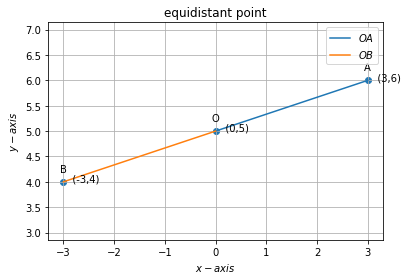
\includegraphics[width=\columnwidth]{./chapters/10/7/1/10/figs/fig.png}
 \end{center}
\caption{}
\label{fig:chapters/10/7/1/10/Fig1}
\end{figure}



\end{enumerate}


\section{Section Formula}
\begin{enumerate}[label=\thesection.\arabic*,ref=\thesection.\theenumi]
\numberwithin{equation}{enumi}
\numberwithin{figure}{enumi}
\numberwithin{table}{enumi}

\item Find the coordinates of the point which divides the join of $(-1,7) \text{ and } (4,-3)$ in the ratio 2:3.
	\\
		\solution
	\iffalse
\documentclass[12pt]{article}
\usepackage{graphicx}
\usepackage{amsmath}
\usepackage{mathtools}
\usepackage{gensymb}

\newcommand{\mydet}[1]{\ensuremath{\begin{vmatrix}#1\end{vmatrix}}}
\providecommand{\brak}[1]{\ensuremath{\left(#1\right)}}
\providecommand{\norm}[1]{\left\lVert#1\right\rVert}
\newcommand{\solution}{\noindent \textbf{Solution: }}
\newcommand{\myvec}[1]{\ensuremath{\begin{pmatrix}#1\end{pmatrix}}}
\let\vec\mathbf

\begin{document}
\begin{center}
\textbf\large{CHAPTER-7 \\ COORDINATE GEOMETRY}
\end{center}
\section*{Excercise 7.2}

1. Find the coordinates of the point which divides the join $\vec(-1,7) \text{ and } \vec(4,-3)$ in the ratio 2:3 :
\\
\\
\solution\\		
\fi
The coordinates and ratio are given as
\begin{align}
\vec{P}=\myvec{-1\\7\\},
\vec{Q}=\myvec{4\\-3\\},
n=\frac{3}{2}
\end{align}
Using section formula
\begin{align}
\vec{R}&=\frac{\vec{Q}+n\vec{P}}{1+n}\\
&=\frac{1}{1+\frac{3}{2}}  \myvec{\myvec{
4\\
-3\\
}
  +
   \frac{3}{2}\myvec{
-1\\
7\\
}}\\
&=\myvec{
1\\
3
}
\end{align}
See Fig. 
\ref{fig:chapters/10/7/2/1/Fig}
\begin{figure}[!h]
\begin{center}
   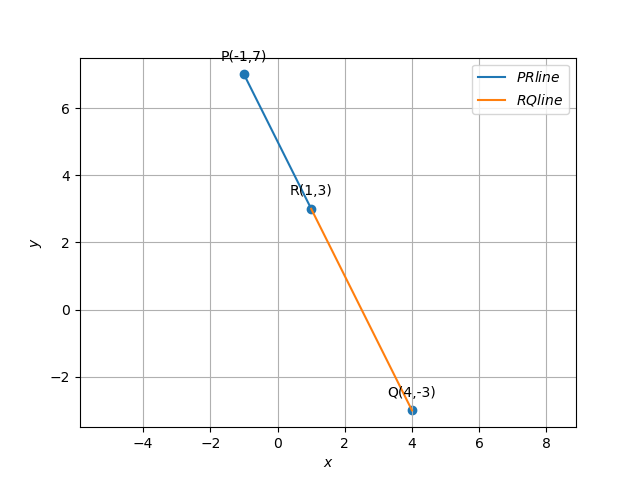
\includegraphics[width=\columnwidth]{chapters/10/7/2/1/figs/linefig.png}
\end{center}
\caption{}
\label{fig:chapters/10/7/2/1/Fig}
\end{figure}


\item Find the coordinates of the points of trisection of the line segment joining $(4,-1) \text{ and } (-2,3)$.
	\\
		\solution
	\iffalse
\documentclass[12pt]{article}
\usepackage{graphicx}
\usepackage[none]{hyphenat}
\usepackage{graphicx}
\usepackage{listings}
\usepackage[english]{babel}
\usepackage{graphicx}
\usepackage{caption} 
\usepackage{booktabs}
\usepackage{array}
\usepackage{amssymb} % for \because
\usepackage{amsmath}   % for having text in math mode
\usepackage{extarrows} % for Row operations arrows
\usepackage{listings}
\usepackage[utf8]{inputenc}
\lstset{
  frame=single,
  breaklines=true
}
\usepackage{hyperref}
  
%Following 2 lines were added to remove the blank page at the beginning
\usepackage{atbegshi}% http://ctan.org/pkg/atbegshi
\AtBeginDocument{\AtBeginShipoutNext{\AtBeginShipoutDiscard}}


%New macro definitions
\newcommand{\mydet}[1]{\ensuremath{\begin{vmatrix}#1\end{vmatrix}}}
\providecommand{\brak}[1]{\ensuremath{\left(#1\right)}}
\newcommand{\solution}{\noindent \textbf{Solution: }}
\newcommand{\myvec}[1]{\ensuremath{\begin{pmatrix}#1\end{pmatrix}}}
\providecommand{\norm}[1]{\left\lVert#1\right\rVert}
\providecommand{\abs}[1]{\left\vert#1\right\vert}
\let\vec\mathbf

\begin{document}

\begin{center}
\title{\textbf{VECTORS}}
\date{\vspace{-5ex}} %Not to print date automatically
\maketitle
\end{center}

\section{10$^{th}$ Maths - EXERCISE-7.2}

\begin{enumerate}
\item Find the coordinates of the points of trisection of the line segment joining $\vec(4 ,-1) \text{ and } \vec(-2,-3)$ 
\end{enumerate}
\fi
Let the given points be
\begin{align}
\vec{Q}=\myvec{4\\ -1} ,
\vec{P}=\myvec{-2\\ -3}
\end{align}
Using section formula
\begin{align}
\vec{R}&=\frac{\vec{Q}+n\vec{P}}{1+n}
\end{align}
Choosing $n = \frac{1}{2}$,
\begin{align}
\vec{R}&=\frac{1}{1+\frac{1}{2}}\brak{\myvec{4\\-1}+\frac{1}{2}\myvec{-2\\-3}}\\
&=\myvec{2\\ \frac{-5}{3}}\\
\end{align}
and choosing $n = 2$
\begin{align}
\vec{S}&=\frac{1}{1+\frac{2}{1}}\brak{\myvec{4\\-1}+\frac{2}{1}\myvec{-2\\-3}}\\
&=\myvec{0\\ \frac{-7}{3}}
\end{align}
which are the desired points of trisection.  These are plotted in Fig. 
		\ref{fig:chapters/10/7/2/2/Figure}
\begin{figure}[h]
\centering
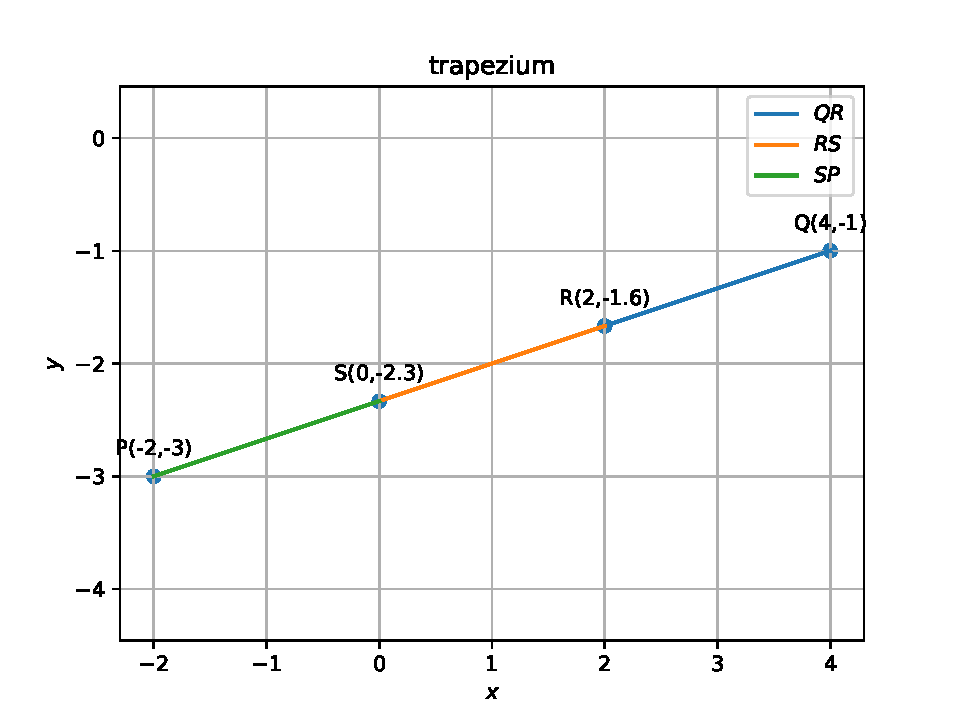
\includegraphics[width=\columnwidth]{chapters/10/7/2/2/figs/dj.pdf}
\caption{}
		\label{fig:chapters/10/7/2/2/Figure}
\end{figure}

\item
	\iffalse
\item To conduct Sports Day activities, in your rectangular shaped school                   
ground ABCD, lines have 
drawn with chalk powder at a                 
distance of 1m each. 100 flower pots have been placed at a distance of 1m 
from each other along AD, as shown 
in Fig. 7.12. Niharika runs $ \frac {1}{4} $th the 
distance AD on the 2nd line and 
posts a green flag. Preet runs $ \frac {1}{5} $th 
the distance AD on the eighth line 
and posts a red flag. What is the 
distance between both the flags? If 
Rashmi has to post a blue flag exactly 
halfway between the line segment 
joining the two flags, where should 
she post her flag?
\begin{figure}[h!]
  \centering
  \includegraphics[width=\columnwidth]{sc.png}
  \caption{}
\label{fig:10/7/12Fig1}
\end{figure}               
\fi
      
\item Find the ratio in which the line segment joining the points $(-3,10) \text{ and } (6,-8)$ $\text{ is divided by } (-1,6)$.
	\\
		\solution
	\iffalse
\documentclass[12pt]{article}
\usepackage{graphicx}
%\documentclass[journal,12pt,twocolumn]{IEEEtran}
\usepackage[none]{hyphenat}
\usepackage{graphicx}
\usepackage{listings}
\usepackage[english]{babel}
\usepackage{graphicx}
\usepackage{caption} 
\usepackage{hyperref}
\usepackage{booktabs}
\def\inputGnumericTable{}
\usepackage{color}                                            %%
    \usepackage{array}                                            %%
    \usepackage{longtable}                                        %%
    \usepackage{calc}                                             %%
    \usepackage{multirow}                                         %%
    \usepackage{hhline}                                           %%
    \usepackage{ifthen}
\usepackage{array}
\usepackage{amsmath}   % for having text in math mode
\usepackage{listings}
\lstset{
language=tex,
frame=single, 
breaklines=true
}
  
%Following 2 lines were added to remove the blank page at the beginning
\usepackage{atbegshi}% http://ctan.org/pkg/atbegshi
\AtBeginDocument{\AtBeginShipoutNext{\AtBeginShipoutDiscard}}
%
%New macro definitions
\newcommand{\mydet}[1]{\ensuremath{\begin{vmatrix}#1\end{vmatrix}}}
\providecommand{\brak}[1]{\ensuremath{\left(#1\right)}}
\providecommand{\norm}[1]{\left\lVert#1\right\rVert}
\newcommand{\solution}{\noindent \textbf{Solution: }}
\newcommand{\myvec}[1]{\ensuremath{\begin{pmatrix}#1\end{pmatrix}}}
\let\vec\mathbf
\begin{document}
\begin{center}
\title{\textbf{Coordinate Geometry}}
\date{\vspace{-5ex}} %Not to print date automatically
\maketitle
\end{center}
\setcounter{page}{1}
\section*{10$^{th}$ Maths - Chapter 7}
This is Problem-4 from Exercise 7.2
\begin{enumerate}
\item Find the ratio in which the line segement joining the points $\myvec{-3 \\ 10}$ and $\myvec{6\\-8}$ is divided by $\myvec{-1\\6}$.\\
\solution \\
\fi
		The input parameters for this problem are available in Table \eqref{tab:10/7/2/4-1}.
\begin{table}[ht!]
%%%%%%%%%%%%%%%%%%%%%%%%%%%%%%%%%%%%%%%%%%%%%%%%%%%%%%%%%%%%%%%%%%%%%%
%%                                                                  %%
%%  This is the header of a LaTeX2e file exported from Gnumeric.    %%
%%                                                                  %%
%%  This file can be compiled as it stands or included in another   %%
%%  LaTeX document. The table is based on the longtable package so  %%
%%  the longtable options (headers, footers...) can be set in the   %%
%%  preamble section below (see PRAMBLE).                           %%
%%                                                                  %%
%%  To include the file in another, the following two lines must be %%
%%  in the including file:                                          %%
%%        \def\inputGnumericTable{}                                 %%
%%  at the beginning of the file and:                               %%
%%        \input{name-of-this-file.tex}                             %%
%%  where the table is to be placed. Note also that the including   %%
%%  file must use the following packages for the table to be        %%
%%  rendered correctly:                                             %%
%%    \usepackage[latin1]{inputenc}                                 %%
%%    \usepackage{color}                                            %%
%%    \usepackage{array}                                            %%
%%    \usepackage{longtable}                                        %%
%%    \usepackage{calc}                                             %%
%%    \usepackage{multirow}                                         %%
%%    \usepackage{hhline}                                           %%
%%    \usepackage{ifthen}                                           %%
%%  optionally (for landscape tables embedded in another document): %%
%%    \usepackage{lscape}                                           %%
%%                                                                  %%
%%%%%%%%%%%%%%%%%%%%%%%%%%%%%%%%%%%%%%%%%%%%%%%%%%%%%%%%%%%%%%%%%%%%%%



%%  This section checks if we are begin input into another file or  %%
%%  the file will be compiled alone. First use a macro taken from   %%
%%  the TeXbook ex 7.7 (suggestion of Han-Wen Nienhuys).            %%
\def\ifundefined#1{\expandafter\ifx\csname#1\endcsname\relax}


%%  Check for the \def token for inputed files. If it is not        %%
%%  defined, the file will be processed as a standalone and the     %%
%%  preamble will be used.                                          %%
\ifundefined{inputGnumericTable}

%%  We must be able to close or not the document at the end.        %%
 \def\gnumericTableEnd{\end{document}}


%%%%%%%%%%%%%%%%%%%%%%%%%%%%%%%%%%%%%%%%%%%%%%%%%%%%%%%%%%%%%%%%%%%%%%
%%                                                                  %%
%%  This is the PREAMBLE. Change these values to get the right      %%
%%  paper size and other niceties.                                  %%
%%                                                                  %%
%%%%%%%%%%%%%%%%%%%%%%%%%%%%%%%%%%%%%%%%%%%%%%%%%%%%%%%%%%%%%%%%%%%%%%

 \documentclass[12pt%
     %,landscape%
                    ]{report}
       \usepackage[latin1]{inputenc}
       \usepackage{fullpage}
       \usepackage{color}
       \usepackage{array}
       \usepackage{longtable}
       \usepackage{calc}
       \usepackage{multirow}
       \usepackage{hhline}
       \usepackage{ifthen}

 \begin{document}


%%  End of the preamble for the standalone. The next section is for %%
%%  documents which are included into other LaTeX2e files.          %%
\else

%%  We are not a stand alone document. For a regular table, we will %%
%%  have no preamble and only define the closing to mean nothing.   %%
    \def\gnumericTableEnd{}

%%  If we want landscape mode in an embedded document, comment out  %%
%%  the line above and uncomment the two below. The table will      %%
%%  begin on a new page and run in landscape mode.                  %%
%       \def\gnumericTableEnd{\end{landscape}}
%       \begin{landscape}


%%  End f theoelse clause for this file being \input.              %%
\fi

%%%%%%%%%%%%%%%%%%%%%%%%%%%%%%%%%%%%%%%%%%%%%%%%%%%%%%%%%%%%%%%%%%%%%%
%%                                                                  %%
%%  The rest is the gnumeric table, except for the closing          %%
%%  statement. Changes below will alter the table's appearance.     %%
%%                                                                  %%
%%%%%%%%%%%%%%%%%%%%%%%%%%%%%%%%%%%%%%%%%%%%%%%%%%%%%%%%%%%%%%%%%%%%%%

\providecommand{\gnumericmathit}[1]{#1} 
%%  Uncomment the next line if you would like your numbers to be in %%
%%  italics if they are italizised in the gnumeric table.           %%
%\renewcommand{\gnumericmathit}[1]{\mathit{#1}}
\providecommand{\gnumericPB}[1]%
{\let\gnumericTemp=\\#1\let\\=\gnumericTemp\hspace{0pt}}
 \ifundefined{gnumericTableWidthDefined}
        \newlength{\gnumericTableWidth}
        \newlength{\gnumericTableWidthComplete}
        \newlength{\gnumericMultiRowLength}
        \global\def\gnumericTableWidthDefined{}
 \fi
%% The following setting protects this code from babel shorthands.  %%
 \ifthenelse{\isundefined{\languageshorthands}}{}{\languageshorthands{english}}
%%  The default table format retains the relative column widths of  %%
%%  gnumeric. They can easily be changed to c, r or l. In that case %%
%%  you may want to comment out the next line and uncomment the one %%
%%  thereafter                                                      %%
\providecommand\gnumbox{\makebox[0pt]}
%%\providecommand\gnumbox[1][]{\makebox}

%% to adjust positions in multirow situations                       %%
\setlength{\bigstrutjot}{\jot}
\setlength{\extrarowheight}{\doublerulesep}

%%  The \setlongtables command keeps column widths the same across  %%
%%  pages. Simply comment out next line for varying column widths.  %%
\setlongtables

\setlength\gnumericTableWidth{%
 53pt+%
 53pt+%
 82pt+%
 53pt+%
0pt}
\def\gumericNumCols{4}
\setlength\gnumericTableWidthComplete{\gnumericTableWidth+%
         \tabcolsep*\gumericNumCols*2+\arrayrulewidth*\gumericNumCols}
\ifthenelse{\lengthtest{\gnumericTableWidthComplete > \linewidth}}%
         {\def\gnumericScale{1*\ratio{\linewidth-%
                        \tabcolsep*\gumericNumCols*2-%
                        \arrayrulewidth*\gumericNumCols}%
{\gnumericTableWidth}}}%
{\def\gnumericScale{1}}

%%%%%%%%%%%%%%%%%%%%%%%%%%%%%%%%%%%%%%%%%%%%%%%%%%%%%%%%%%%%%%%%%%%%%%
%%                                                                  %%
%% The following are the widths of the various columns. We are      %%
%% defining them here because then they are easier to change.       %%
%% Depending on the cell formats we may use them more than once.    %%
%%                                                                  %%
%%%%%%%%%%%%%%%%%%%%%%%%%%%%%%%%%%%%%%%%%%%%%%%%%%%%%%%%%%%%%%%%%%%%%%

\ifthenelse{\isundefined{\gnumericColA}}{\newlength{\gnumericColA}}{}\settowidth{\gnumericColA}{\begin{tabular}{@{}p{53pt*\gnumericScale}@{}}x\end{tabular}}
\ifthenelse{\isundefined{\gnumericColB}}{\newlength{\gnumericColB}}{}\settowidth{\gnumericColB}{\begin{tabular}{@{}p{53pt*\gnumericScale}@{}}x\end{tabular}}
\ifthenelse{\isundefined{\gnumericColC}}{\newlength{\gnumericColC}}{}\settowidth{\gnumericColC}{\begin{tabular}{@{}p{82pt*\gnumericScale}@{}}x\end{tabular}}
\ifthenelse{\isundefined{\gnumericColD}}{\newlength{\gnumericColD}}{}\settowidth{\gnumericColD}{\begin{tabular}{@{}p{53pt*\gnumericScale}@{}}x\end{tabular}}

\begin{center}
\begin{tabular}[c]{%
 b{\gnumericColA}%
 b{\gnumericColB}%
 b{\gnumericColC}%
 b{\gnumericColD}%
 }

%%%%%%%%%%%%%%%%%%%%%%%%%%%%%%%%%%%%%%%%%%%%%%%%%%%%%%%%%%%%%%%%%%%%%%
%%  The longtable options. (Caption, headers... see Goosens, p.124) %%
% \caption{The Table Caption.}             \\ %
% \hline % Across the top of the table.
%%  The rest of these options are table rows which are placed on    %%
%%  the first, last or every page. Use \multicolumn if you want.    %%

%%  Header for the first page.                                      %%
% \multicolumn{4}{c}{The First Header} \\ \hline 
% \multicolumn{1}{c}{colTag} %Column 1
% &\multicolumn{1}{c}{colTag} %Column 2
% &\multicolumn{1}{c}{colTag} %Column 3
% &\multicolumn{1}{c}{colTag} \\ \hline %Last column
% \endfirsthead

%%  The running header definition.                                  %%
% \hline
% \multicolumn{4}{l}{\ldots\small\slshape continued} \\ \hline
% \multicolumn{1}{c}{colTag} %Column 1
% &\multicolumn{1}{c}{colTag} %Column 2
% &\multicolumn{1}{c}{colTag} %Column 3
% &\multicolumn{1}{c}{colTag} \\ \hline %Last column
% \endhead

%%  The running footer definition.                                  %%
% \hline
% \multicolumn{4}{r}{\small\slshape continued\ldots} \\
% \endfoot

%%  The ending footer definition.                                   %%
% \multicolumn{4}{c}{That's all folks} \\ \hline 
% \endlastfoot
%%%%%%%%%%%%%%%%%%%%%%%%%%%%%%%%%%%%%%%%%%%%%%%%%%%%%%%%%%%%%%%%%%%%%%

\hhline{|-|-|-~}
  \multicolumn{1}{|p{\gnumericColA}|}%
 {\gnumericPB{\centering}\gnumbox{\textbf{Symbol}}}
 &\multicolumn{1}{p{\gnumericColB}|}%
 {\gnumericPB{\centering}\gnumbox{\textbf{Value}}}
 &\multicolumn{1}{p{\gnumericColC}|}%
 {\gnumericPB{\centering}\gnumbox{\textbf{Description}}}
 &
\\
\hhline{|---|~}
  \multicolumn{1}{|p{\gnumericColA}|}%
 {\gnumericPB{\centering}\gnumbox{$\vec{P}$}}
 &\multicolumn{1}{p{\gnumericColB}|}%
 {\gnumericPB{\centering}\gnumbox{$\myvec{-3\\10}$}}
 &\multicolumn{1}{p{\gnumericColC}|}%
 {\gnumericPB{\centering}\gnumbox{First point}}
 &
\\
\hhline{|---|~}
  \multicolumn{1}{|p{\gnumericColA}|}%
 {\gnumericPB{\centering}\gnumbox{$\vec{Q}$}}
 &\multicolumn{1}{p{\gnumericColB}|}%
 {\gnumericPB{\centering}\gnumbox{$\myvec{6\\-8}$}}
 &\multicolumn{1}{p{\gnumericColC}|}%
 {\gnumericPB{\centering}\gnumbox{Second point}}
 &
\\
\hhline{|---|~}
  \multicolumn{1}{|p{\gnumericColA}|}%
 {\gnumericPB{\centering}\gnumbox{$\vec{R}$}}
 &\multicolumn{1}{p{\gnumericColB}|}%
 {\gnumericPB{\centering}\gnumbox{$\myvec{-1\\6}$}}
 &\multicolumn{1}{p{\gnumericColC}|}%
 {\gnumericPB{\centering}\gnumbox{Desired point}}
 &
\\
\hhline{|-|-|-|~}
\end{tabular}
 \end{center}

\ifthenelse{\isundefined{\languageshorthands}}{}{\languageshorthands{\languagename}}
\gnumericTableEnd

\caption{}
\label{tab:10/7/2/4-1} 
\end{table}
Using section formula,
\begin{align}
         \vec{R} &=\frac{\vec{Q}+n\vec{P}}{1+n}\label{eq:chapters/10/7/2/4/1}
\end{align}
Substituting the values of $\vec{P},\vec{Q}$ and $\vec{R}$ in \eqref{eq:chapters/10/7/2/4/1}
\begin{align}
         \myvec{-1\\6} &=\frac{{\myvec{-3\\10}+n\myvec{6\\-8}}}{1+n}\\
 &=\frac{1}{1+n}\brak{{\myvec{-3\\10}+n\myvec{6\\-8}}} \\
 &=\frac{1}{1+n}\myvec{-3+6n\\10-8n} \label{eq:chapters/10/7/2/4/4}
\end{align}
Simplifying \eqref{eq:chapters/10/7/2/4/4} yeilds,
\begin{align}
          -1 &=\frac{-3+6n}{1+n}\\
\implies          n &=\frac{2}{7}
\end{align}
Also,
\begin{align}
          6 &=\frac{10-8n}{1+n}\\
    \implies      n &=\frac{2}{7}
\end{align}
Hence the desired ratio is $\dfrac{2}{7}$.  
\begin{figure}[!h]
 \begin{center}
  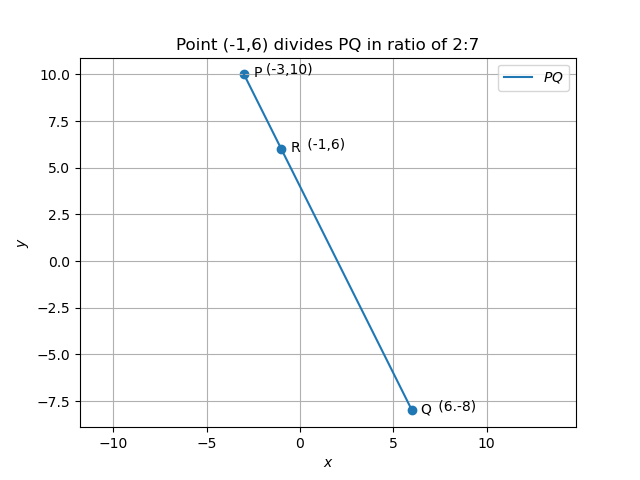
\includegraphics[width=\columnwidth]{chapters/10/7/2/4/figs/fig.png}
 \end{center}
\caption{}
\label{fig:10/7/2/4Fig1}
\end{figure}

\item Find the ratio in which the line segment joining $A(1,-5) \text{ and } B(-4,5)$ $\text{is divided by the x-axis}$. Also find the coordinates of the point of division.
\item If $(1,2), (4,y), (x,6), (3,5)$ are the vertices of a parallelogram taken in order, find x and y.
	\\
		\solution
	\iffalse
\documentclass[12pt]{article}
\usepackage{graphicx}
%\documentclass[journal,12pt,twocolumn]{IEEEtran}
\def\inputGnumericTable{}
\usepackage{color}                                            %%
    \usepackage{array}                                            %%
    \usepackage{longtable}                                        %%
    \usepackage{calc}                                             %%
    \usepackage{multirow}                                         %%
    \usepackage{hhline}                                           %%
    \usepackage{ifthen}
\usepackage[none]{hyphenat}
\usepackage{graphicx}
\usepackage{listings}
\usepackage[english]{babel}
\usepackage{graphicx}
\usepackage{caption} 
\usepackage{hyperref}
\usepackage{booktabs}
\usepackage{array}
\usepackage{amsmath}   % for having text in math mode
\usepackage{listings}
\lstset{
  frame=single,
  breaklines=true
}
  
%Following 2 lines were added to remove the blank page at the beginning
\usepackage{atbegshi}% http://ctan.org/pkg/atbegshi
\AtBeginDocument{\AtBeginShipoutNext{\AtBeginShipoutDiscard}}
%


%New macro definitions
\newcommand{\mydet}[1]{\ensuremath{\begin{vmatrix}#1\end{vmatrix}}}
\providecommand{\brak}[1]{\ensuremath{\left(#1\right)}}
\providecommand{\norm}[1]{\left\lVert#1\right\rVert}
\newcommand{\solution}{\noindent \textbf{Solution: }}
\newcommand{\myvec}[1]{\ensuremath{\begin{pmatrix}#1\end{pmatrix}}}
\let\vec\mathbf

\begin{document}

\begin{center}
\title{\textbf{Properties of Parallelegram}}
\date{\vspace{-5ex}} %Not to print date automatically
\maketitle
\end{center}

\setcounter{page}{1}

\section{10$^{th}$ Maths - Chapter 7}

This is Problem-6 from Exercise 7.2

\begin{enumerate}
\item If $\vec{A}(1, 2),\vec{B}(4, x),\vec{C}(y, 6) \text{and } \vec{D}(3, 5)$ are the vertices of a parallelogram taken in order,find x and y.
\end{enumerate}
\fi

The input parameters for this problem are available in
\ref{table:chapters/10/7/2/6/tables/}.	
\begin{table}[!ht]
	\centering
	%%%%%%%%%%%%%%%%%%%%%%%%%%%%%%%%%%%%%%%%%%%%%%%%%%%%%%%%%%%%%%%%%%%%%%
%%                                                                  %%
%%  This is the header of a LaTeX2e file exported from Gnumeric.    %%
%%                                                                  %%
%%  This file can be compiled as it stands or included in another   %%
%%  LaTeX document. The table is based on the longtable package so  %%
%%  the longtable options (headers, footers...) can be set in the   %%
%%  preamble section below (see PRAMBLE).                           %%
%%                                                                  %%
%%  To include the file in another, the following two lines must be %%
%%  in the including file:                                          %%
%%        \def\inputGnumericTable{}                                 %%
%%  at the beginning of the file and:                               %%
%%        \input{name-of-this-file.tex}                             %%
%%  where the table is to be placed. Note also that the including   %%
%%  file must use the following packages for the table to be        %%
%%  rendered correctly:                                             %%
%%    \usepackage[latin1]{inputenc}                                 %%
%%    \usepackage{color}                                            %%
%%    \usepackage{array}                                            %%
%%    \usepackage{longtable}                                        %%
%%    \usepackage{calc}                                             %%
%%    \usepackage{multirow}                                         %%
%%    \usepackage{hhline}                                           %%
%%    \usepackage{ifthen}                                           %%
%%  optionally (for landscape tables embedded in another document): %%
%%    \usepackage{lscape}                                           %%
%%                                                                  %%
%%%%%%%%%%%%%%%%%%%%%%%%%%%%%%%%%%%%%%%%%%%%%%%%%%%%%%%%%%%%%%%%%%%%%%



%%  This section checks if we are begin input into another file or  %%
%%  the file will be compiled alone. First use a macro taken from   %%
%%  the TeXbook ex 7.7 (suggestion of Han-Wen Nienhuys).            %%
\def\ifundefined#1{\expandafter\ifx\csname#1\endcsname\relax}


%%  Check for the \def token for inputed files. If it is not        %%
%%  defined, the file will be processed as a standalone and the     %%
%%  preamble will be used.                                          %%
\ifundefined{inputGnumericTable}

%%  We must be able to close or not the document at the end.        %%
	\def\gnumericTableEnd{\end{document}}


%%%%%%%%%%%%%%%%%%%%%%%%%%%%%%%%%%%%%%%%%%%%%%%%%%%%%%%%%%%%%%%%%%%%%%
%%                                                                  %%
%%  This is the PREAMBLE. Change these values to get the right      %%
%%  paper size and other niceties.                                  %%
%%                                                                  %%
%%%%%%%%%%%%%%%%%%%%%%%%%%%%%%%%%%%%%%%%%%%%%%%%%%%%%%%%%%%%%%%%%%%%%%

	\documentclass[12pt%
			  %,landscape%
                    ]{report}
       \usepackage[latin1]{inputenc}
       \usepackage{fullpage}
       \usepackage{color}
       \usepackage{array}
       \usepackage{longtable}
       \usepackage{calc}
       \usepackage{multirow}
       \usepackage{hhline}
       \usepackage{ifthen}

	\begin{document}


%%  End of the preamble for the standalone. The next section is for %%
%%  documents which are included into other LaTeX2e files.          %%
\else

%%  We are not a stand alone document. For a regular table, we will %%
%%  have no preamble and only define the closing to mean nothing.   %%
    \def\gnumericTableEnd{}

%%  If we want landscape mode in an embedded document, comment out  %%
%%  the line above and uncomment the two below. The table will      %%
%%  begin on a new page and run in landscape mode.                  %%
%       \def\gnumericTableEnd{\end{landscape}}
%       \begin{landscape}


%%  End of the else clause for this file being \input.              %%
\fi

%%%%%%%%%%%%%%%%%%%%%%%%%%%%%%%%%%%%%%%%%%%%%%%%%%%%%%%%%%%%%%%%%%%%%%
%%                                                                  %%
%%  The rest is the gnumeric table, except for the closing          %%
%%  statement. Changes below will alter the table's appearance.     %%
%%                                                                  %%
%%%%%%%%%%%%%%%%%%%%%%%%%%%%%%%%%%%%%%%%%%%%%%%%%%%%%%%%%%%%%%%%%%%%%%

\providecommand{\gnumericmathit}[1]{#1} 
%%  Uncomment the next line if you would like your numbers to be in %%
%%  italics if they are italizised in the gnumeric table.           %%
%\renewcommand{\gnumericmathit}[1]{\mathit{#1}}
\providecommand{\gnumericPB}[1]%
{\let\gnumericTemp=\\#1\let\\=\gnumericTemp\hspace{0pt}}
 \ifundefined{gnumericTableWidthDefined}
        \newlength{\gnumericTableWidth}
        \newlength{\gnumericTableWidthComplete}
        \newlength{\gnumericMultiRowLength}
        \global\def\gnumericTableWidthDefined{}
 \fi
%% The following setting protects this code from babel shorthands.  %%
 \ifthenelse{\isundefined{\languageshorthands}}{}{\languageshorthands{english}}
%%  The default table format retains the relative column widths of  %%
%%  gnumeric. They can easily be changed to c, r or l. In that case %%
%%  you may want to comment out the next line and uncomment the one %%
%%  thereafter                                                      %%
\providecommand\gnumbox{\makebox[0pt]}
%%\providecommand\gnumbox[1][]{\makebox}

%% to adjust positions in multirow situations                       %%
\setlength{\bigstrutjot}{\jot}
\setlength{\extrarowheight}{\doublerulesep}

%%  The \setlongtables command keeps column widths the same across  %%
%%  pages. Simply comment out next line for varying column widths.  %%
\setlongtables

\setlength\gnumericTableWidth{%
	53pt+%
	53pt+%
	82pt+%
	53pt+%
0pt}
\def\gumericNumCols{4}
\setlength\gnumericTableWidthComplete{\gnumericTableWidth+%
         \tabcolsep*\gumericNumCols*2+\arrayrulewidth*\gumericNumCols}
\ifthenelse{\lengthtest{\gnumericTableWidthComplete > \linewidth}}%
         {\def\gnumericScale{1*\ratio{\linewidth-%
                        \tabcolsep*\gumericNumCols*2-%
                        \arrayrulewidth*\gumericNumCols}%
{\gnumericTableWidth}}}%
{\def\gnumericScale{1}}

%%%%%%%%%%%%%%%%%%%%%%%%%%%%%%%%%%%%%%%%%%%%%%%%%%%%%%%%%%%%%%%%%%%%%%
%%                                                                  %%
%% The following are the widths of the various columns. We are      %%
%% defining them here because then they are easier to change.       %%
%% Depending on the cell formats we may use them more than once.    %%
%%                                                                  %%
%%%%%%%%%%%%%%%%%%%%%%%%%%%%%%%%%%%%%%%%%%%%%%%%%%%%%%%%%%%%%%%%%%%%%%

\ifthenelse{\isundefined{\gnumericColA}}{\newlength{\gnumericColA}}{}\settowidth{\gnumericColA}{\begin{tabular}{@{}p{53pt*\gnumericScale}@{}}x\end{tabular}}
\ifthenelse{\isundefined{\gnumericColB}}{\newlength{\gnumericColB}}{}\settowidth{\gnumericColB}{\begin{tabular}{@{}p{53pt*\gnumericScale}@{}}x\end{tabular}}
\ifthenelse{\isundefined{\gnumericColC}}{\newlength{\gnumericColC}}{}\settowidth{\gnumericColC}{\begin{tabular}{@{}p{82pt*\gnumericScale}@{}}x\end{tabular}}
\ifthenelse{\isundefined{\gnumericColD}}{\newlength{\gnumericColD}}{}\settowidth{\gnumericColD}{\begin{tabular}{@{}p{53pt*\gnumericScale}@{}}x\end{tabular}}

	\begin{center}
\begin{tabular}[c]{%
	b{\gnumericColA}%
	b{\gnumericColB}%
	b{\gnumericColC}%
	b{\gnumericColD}%
	}

%%%%%%%%%%%%%%%%%%%%%%%%%%%%%%%%%%%%%%%%%%%%%%%%%%%%%%%%%%%%%%%%%%%%%%
%%  The longtable options. (Caption, headers... see Goosens, p.124) %%
%	\caption{The Table Caption.}             \\	%
% \hline	% Across the top of the table.
%%  The rest of these options are table rows which are placed on    %%
%%  the first, last or every page. Use \multicolumn if you want.    %%

%%  Header for the first page.                                      %%
%	\multicolumn{4}{c}{The First Header} \\ \hline 
%	\multicolumn{1}{c}{colTag}	%Column 1
%	&\multicolumn{1}{c}{colTag}	%Column 2
%	&\multicolumn{1}{c}{colTag}	%Column 3
%	&\multicolumn{1}{c}{colTag}	\\ \hline %Last column
%	\endfirsthead

%%  The running header definition.                                  %%
%	\hline
%	\multicolumn{4}{l}{\ldots\small\slshape continued} \\ \hline
%	\multicolumn{1}{c}{colTag}	%Column 1
%	&\multicolumn{1}{c}{colTag}	%Column 2
%	&\multicolumn{1}{c}{colTag}	%Column 3
%	&\multicolumn{1}{c}{colTag}	\\ \hline %Last column
%	\endhead

%%  The running footer definition.                                  %%
%	\hline
%	\multicolumn{4}{r}{\small\slshape continued\ldots} \\
%	\endfoot

%%  The ending footer definition.                                   %%
%	\multicolumn{4}{c}{That's all folks} \\ \hline 
%	\endlastfoot
%%%%%%%%%%%%%%%%%%%%%%%%%%%%%%%%%%%%%%%%%%%%%%%%%%%%%%%%%%%%%%%%%%%%%%

\hhline{|-|-|-~}
	 \multicolumn{1}{|p{\gnumericColA}|}%
	{\gnumericPB{\centering}\gnumbox{\textbf{Symbol}}}
	&\multicolumn{1}{p{\gnumericColB}|}%
	{\gnumericPB{\centering}\gnumbox{\textbf{Value}}}
	&\multicolumn{1}{p{\gnumericColC}|}%
	{\gnumericPB{\centering}\gnumbox{\textbf{Description}}}
	&
\\
\hhline{|---|~}
	 \multicolumn{1}{|p{\gnumericColA}|}%
	{\gnumericPB{\centering}\gnumbox{$\vec{A}$}}
	&\multicolumn{1}{p{\gnumericColB}|}%
	{\gnumericPB{\centering}\gnumbox{$\myvec{1\\2}$}}
	&\multicolumn{1}{p{\gnumericColC}|}%
	{\gnumericPB{\centering}\gnumbox{First point}}
	&
\\
\hhline{|---|~}
	 \multicolumn{1}{|p{\gnumericColA}|}%
	{\gnumericPB{\centering}\gnumbox{$\vec{B}$}}
	&\multicolumn{1}{p{\gnumericColB}|}%
	{\gnumericPB{\centering}\gnumbox{$\myvec{4\\y}$}}
	&\multicolumn{1}{p{\gnumericColC}|}%
	{\gnumericPB{\centering}\gnumbox{Second point}}
	&
\\
\hhline{|---|~}
	 \multicolumn{1}{|p{\gnumericColA}|}%
	{\gnumericPB{\centering}\gnumbox{$\vec{C}$}}
	&\multicolumn{1}{p{\gnumericColB}|}%
	{\gnumericPB{\centering}\gnumbox{$\myvec{x\\6}$}}
	&\multicolumn{1}{p{\gnumericColC}|}%
	{\gnumericPB{\centering}\gnumbox{Third point}}
	&
\\
\hhline{|---|~}
	 \multicolumn{1}{|p{\gnumericColA}|}%
	{\gnumericPB{\centering}\gnumbox{$\vec{D}$}}
	&\multicolumn{1}{p{\gnumericColB}|}%
	{\gnumericPB{\centering}\gnumbox{$\myvec{3\\5}$}}
	&\multicolumn{1}{p{\gnumericColC}|}%
	{\gnumericPB{\centering}\gnumbox{Fourth point}}
	&
\\

\hhline{|-|-|-|~}
\end{tabular}
	\end{center}

\ifthenelse{\isundefined{\languageshorthands}}{}{\languageshorthands{\languagename}}
\gnumericTableEnd

\caption{}
\label{table:chapters/10/7/2/6/tables/}	
\end{table}
From the given information,
\begin{align}
  \label{eq:chapters/10/7/2/6/tables/det2f}
	\vec{B}-\vec{A} &= \myvec{4 \\y } - \myvec{1 \\2 }  = \myvec{3 \\y-2 }\\
	\vec{C}-\vec{D} &= \myvec{x \\6 } - \myvec{3 \\5 }  = \myvec{x-3 \\1}
\end{align}
Since $ABCD$ is a parallellogram,
\begin{align}
	\myvec{3\\y-2}&=\myvec{x-3\\1}\\
	\implies x&=6 ,y=3
\end{align}
Fig. \ref{fig:chapters/10/7/2/6/Fig3}
provides a verification.
\begin{figure}[h!]
	\begin{center}
  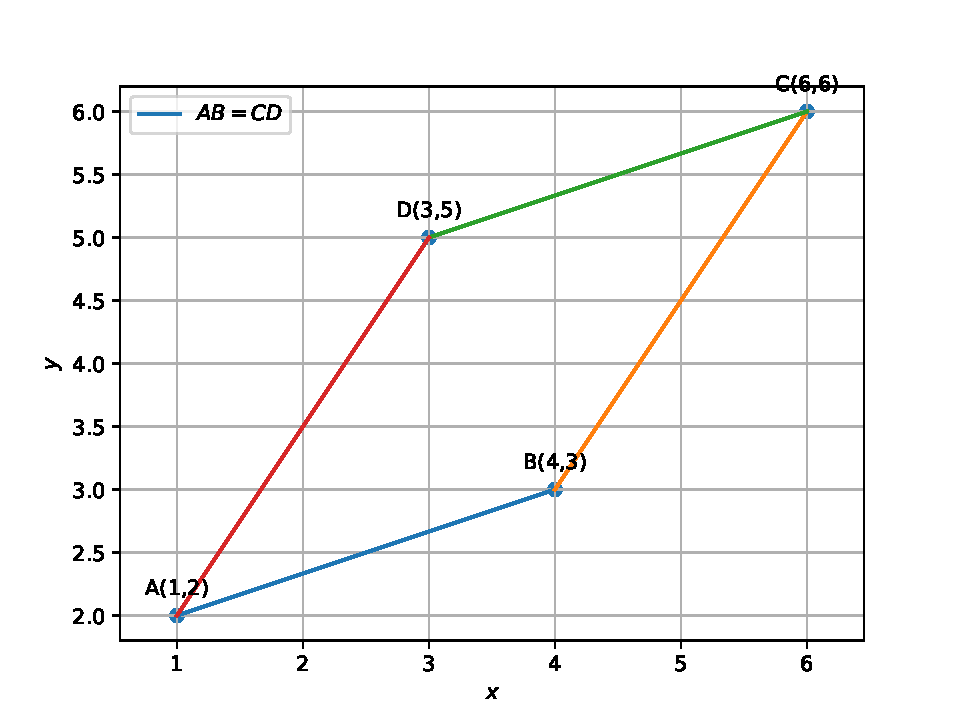
\includegraphics[width=\columnwidth]{chapters/10/7/2/6/figs/para.pdf}
	\end{center}
\caption{}
\label{fig:chapters/10/7/2/6/Fig3}
\end{figure}


\item Find the coordinates of a point A, where AB is the diameter of a circle whose centre is $(2,-3) \text{ and }$ B is $(1,4)$.
	\\
		\solution
	\iffalse
\documentclass[12pt]{article}
\usepackage{graphicx}
\usepackage{amsmath}
\usepackage{mathtools}
\usepackage{gensymb}

\newcommand{\mydet}[1]{\ensuremath{\begin{vmatrix}#1\end{vmatrix}}}
\providecommand{\brak}[1]{\ensuremath{\left(#1\right)}}
\providecommand{\norm}[1]{\left\lVert#1\right\rVert}
\newcommand{\solution}{\noindent \textbf{Solution: }}
\newcommand{\myvec}[1]{\ensuremath{\begin{pmatrix}#1\end{pmatrix}}}
\let\vec\mathbf

\begin{document}
\begin{center}
\section*{CHAPTER 7 - COORDINATE GEOMETRY}

\end{center}
\section*{Excercise 7.2}

Q7.Find the coordinates of point $\vec{A}$, where AB is the diameter of a circle where the center is (2,-3) and $\vec{B}$ is the point (1,4):

\solution
\begin{enumerate}
\item The coordinates $\vec{B}$ and center $\vec{C}$ are given, where:
	\fi
	Let
	\begin{align}
	\vec{B} = \myvec{
		1\\
	    4\\
		},
	\vec{C} = \myvec{
	    2\\
	   -3\\
		}
	\end{align}
	\iffalse
Let us assume the coordinates of $\vec{A}$. Now, $\vec{C}$ is the center which is midpoint of line AB and $\vec{B}$ is one of the coordinate of diameter AB of a circle.
	\fi	
Hence,	
	\begin{align}
	\vec{C} &= \frac{\vec{A+B}}{2} \\
\implies	2\vec{C} &= \vec{A}+\vec{B} \\
		\text{or, }	\vec{A} &= 2\vec{C}-\vec{B} \\
	 &= \myvec{3\\-10\\}	
	\end{align}       
	See Fig. 
\ref{fig:chapters/10/7/2/7Fig}.
\begin{figure}[!h]
\begin{center}	
	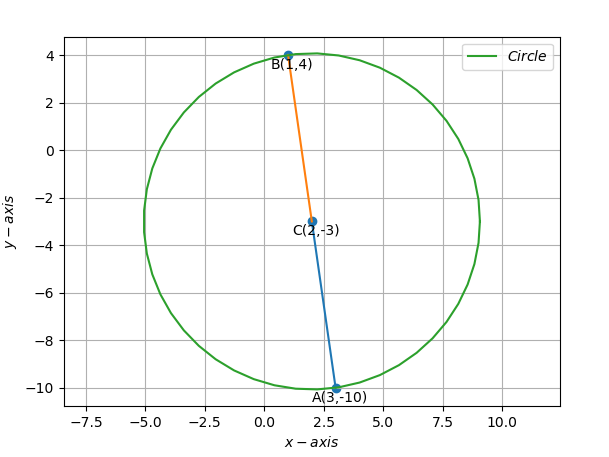
\includegraphics[width=\columnwidth]{chapters/10/7/2/7/figs/Vector1.png}
\end{center}
\caption{}
\label{fig:chapters/10/7/2/7Fig}
\end{figure}
	

\item If A \text{ and } B are $(-2,-2) \text{ and } (2,-4)$, respectively, find the coordinates of P such that AP= $\frac {3}{7}$AB $\text{ and }$ P lies on the line segment AB.
	\\
		\solution
	\iffalse
\documentclass[journal,10pt,twocolumn]{article}
\usepackage{graphicx}
\usepackage[none]{hyphenat}
\usepackage{graphicx}
\usepackage{listings}
\usepackage[english]{babel}
\usepackage{graphicx}
\usepackage{caption} 
\usepackage{booktabs}
\usepackage{array}
\usepackage{amssymb} % for \because
\usepackage{amsmath}   % for having text in math mode
\usepackage{extarrows} % for Row operations arrows
\usepackage{listings}
\usepackage[utf8]{inputenc}
\lstset{
  frame=single,
  breaklines=true
}
\usepackage{hyperref}
  
%Following 2 lines were added to remove the blank page at the beginning
\usepackage{atbegshi}% http://ctan.org/pkg/atbegshi
\AtBeginDocument{\AtBeginShipoutNext{\AtBeginShipoutDiscard}}


%New macro definitions
\newcommand{\mydet}[1]{\ensuremath{\begin{vmatrix}#1\end{vmatrix}}}
\providecommand{\brak}[1]{\ensuremath{\left(#1\right)}}
\newcommand{\solution}{\noindent \textbf{Solution: }}
\newcommand{\myvec}[1]{\ensuremath{\begin{pmatrix}#1\end{pmatrix}}}
\providecommand{\norm}[1]{\left\lVert#1\right\rVert}
\providecommand{\abs}[1]{\left\vert#1\right\vert}
\let\vec\mathbf

\begin{document}

\begin{center}
\title{\textbf{VECTORS}}
\date{\vspace{-5ex}} %Not to print date automatically
\maketitle
\end{center}

\section{10$^{th}$ Maths - EXERCISE-7.2}

\begin{enumerate}
\item If A and B are $(– 2, – 2)\text{ and }(2, – 4)$, respectively, find the coordinates of P such that $AP =\frac{3}{7}AB$ and P lies on the line segment AB. 

\section{SOLUTION}
Given points are
\begin{align}
\vec{A}=\myvec{-2\\ -2} ,
\vec{B}=\myvec{2\\ -4}
\end{align}
The equation of the formula is
\fi
Using section formula, 
\begin{align}
\vec{P}&=\frac{\vec{A}+n\vec{B}}{1+n}
\end{align}
where
\begin{align}
	n =\frac{3}{4}
\end{align}
Thus,
\begin{align}
\vec{P}&=\frac{1}{1+\frac{3}{4}}\brak{\myvec{-2\\-2}+\frac{3}{4}\myvec{2\\-4}}\\
&=\myvec{\frac{-2}{7}\\[1pt] \frac{-20}{7}}
\end{align}
See Fig. 
   \ref{fig:chapters/10/7/2/8/vec.png}
\begin{figure}
   \centering 
 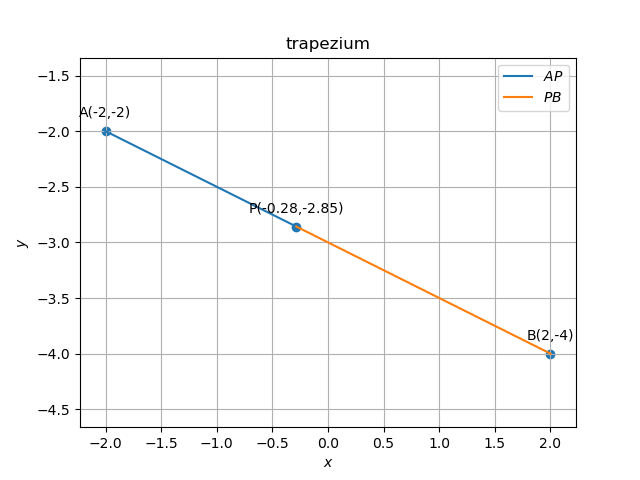
\includegraphics[width=\columnwidth]{chapters/10/7/2/8/figs/vec.png}
   \caption{}
   \label{fig:chapters/10/7/2/8/vec.png}
   \end{figure}

\item Find the coordinates of the points which divide the line segment joining $A(-2,2) \text{ and } B(2,8)$ into four equal parts.
	\\
		\solution
	\iffalse
\documentclass[12pt]{article}
\usepackage{graphicx}
\usepackage{amsmath}
\usepackage{mathtools}
\usepackage{gensymb}
\usepackage[latin1]{inputenc}
\usepackage{fullpage}
\usepackage{color}
\usepackage{array}
\usepackage{longtable}
\usepackage{calc}
\usepackage{multirow}
\usepackage{hhline}
\usepackage{ifthen}
\def\inputGnumericTable{}
\newcommand{\mydet}[1]{\ensuremath{\begin{vmatrix}#1\end{vmatrix}}}
\providecommand{\brak}[1]{\ensuremath{\left(#1\right)}}
\providecommand{\norm}[1]{\left\lVert#1\right\rVert}
\newcommand{\solution}{\noindent \textbf{Solution: }}
\newcommand{\myvec}[1]{\ensuremath{\begin{pmatrix}#1\end{pmatrix}}}
\let\vec\mathbf

\begin{document}
\begin{center}
\textbf\large{CHAPTER-7 \\ COORDINATE GEOMETRY}
\end{center}
\section*{Excercise 10.7.2.9}

1. Find the coordinates of the point which divides the line segment joining $\vec(-2,2) \text{ and } \vec(2,8)$ into four equal parts
\\
\solution\\		
\fi
Let 
\begin{align}
\vec{A}=\myvec{-2\\2\\},
\vec{B}=\myvec{2\\8\\},
\end{align}
Using section formula 
\begin{align}
\vec{R}_i&=\frac{\vec{B}+n\vec{A}}{1+n}
\end{align}

\begin{enumerate}

\item $n = 3$
    
\begin{align}
\vec{R}_1=
\myvec{
-1\\
\\
\frac{7}{2}\\
}
\end{align}

\item $n = 1$
\begin{align}
\vec{R}_2
=\myvec{
0\\
5
}
\end{align}

\item $n=\frac{1}{3}$
\begin{align}
\vec{R}_3
=\myvec{
1\\
\\
\frac{13}{2}\\
}
\end{align}

\end{enumerate}
See Fig. 
\ref{fig:chapters/10/7/2/9/Fig}
\begin{figure}[!h]
\begin{center}
   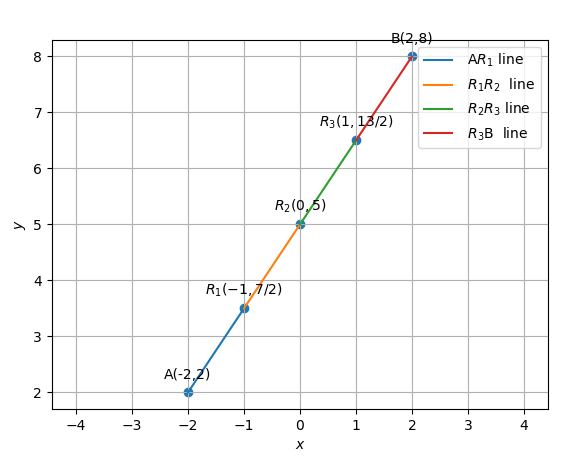
\includegraphics[width=\columnwidth]{chapters/10/7/2/9/figs/10.7.2.9.png}
\end{center}
\caption{}
\label{fig:chapters/10/7/2/9/Fig}
\end{figure}


\item Find the area of a rhombus if its vertices are $(3,0), (4,5), (-1,4) \text{ and } (-2,-1)$ taken in order. [$\vec{Hint}$ : Area of rhombus =$\frac {1}{2}$(product of its diagonals)]
	\\
		\solution
	\iffalse
\documentclass[12pt]{article}
\usepackage{graphicx}
%\documentclass[journal,12pt,twocolumn]{IEEEtran}
\usepackage[none]{hyphenat}
\usepackage{graphicx}
\usepackage{listings}
\usepackage[english]{babel}
\usepackage{graphicx}
\usepackage{caption} 
\usepackage{hyperref}
\usepackage{booktabs}
\def\inputGnumericTable{}
\usepackage{color}                                            %%
    \usepackage{array}                                            %%
    \usepackage{longtable}                                        %%
    \usepackage{calc}                                             %%
    \usepackage{multirow}                                         %%
    \usepackage{hhline}                                           %%
    \usepackage{ifthen}
\usepackage{array}
\usepackage{amsmath}   % for having text in math mode
\usepackage{listings}
\lstset{
language=tex,
frame=single, 
breaklines=true
}
  
%Following 2 lines were added to remove the blank page at the beginning
\usepackage{atbegshi}% http://ctan.org/pkg/atbegshi
\AtBeginDocument{\AtBeginShipoutNext{\AtBeginShipoutDiscard}}
%


%New macro definitions
\newcommand{\mydet}[1]{\ensuremath{\begin{vmatrix}#1\end{vmatrix}}}
\providecommand{\brak}[1]{\ensuremath{\left(#1\right)}}
\providecommand{\norm}[1]{\left\lVert#1\right\rVert}
\newcommand{\solution}{\noindent \textbf{Solution: }}
\newcommand{\myvec}[1]{\ensuremath{\begin{pmatrix}#1\end{pmatrix}}}
\let\vec\mathbf

\begin{document}

\begin{center}
\title{\textbf{Coordinate Geometry}}
\date{\vspace{-5ex}} %Not to print date automatically
\maketitle
\end{center}

\setcounter{page}{1}



\begin{enumerate}

\item\textbf{Problem statement :} Find the area of a rhombus of its vertices are $\myvec{3 ,0}$, $\myvec{4 ,5}$, $\myvec{-1 ,4}$ and $\myvec{-2 ,-1}$taken in order

\solution \\
\fi
The input vertices for this problem are given as
	\begin{align}
	\vec{A} = \myvec{
		3\\
		0
		},
	\vec{B} = \myvec{
		4\\
		5
		},
        \vec{C} = \myvec{
		-1\\
		4
		},
        \vec{D} = \myvec{
		-2\\
		-1
		}
	\end{align}
Since		
\begin{align}
 \vec{A-D}= \myvec{3 \\ 0} - \myvec{-2 \\-1}= \myvec{5\\1}
 \\
  \vec{B-A}= \myvec{4 \\ 5} - \myvec{3 \\0}= \myvec{1\\5}
\end{align}
the area of the rhombus is
\begin{align}
                \norm{\myvec{\vec{A-D}}\times \myvec{\vec{B-A}}}=\mydet{5 & 1\\1 & 5} = 24
\end{align}
See Fig. 
\ref{fig:chapters/10/7/2/10/gFig1}.
\begin{figure}[!h]
 \begin{center}
  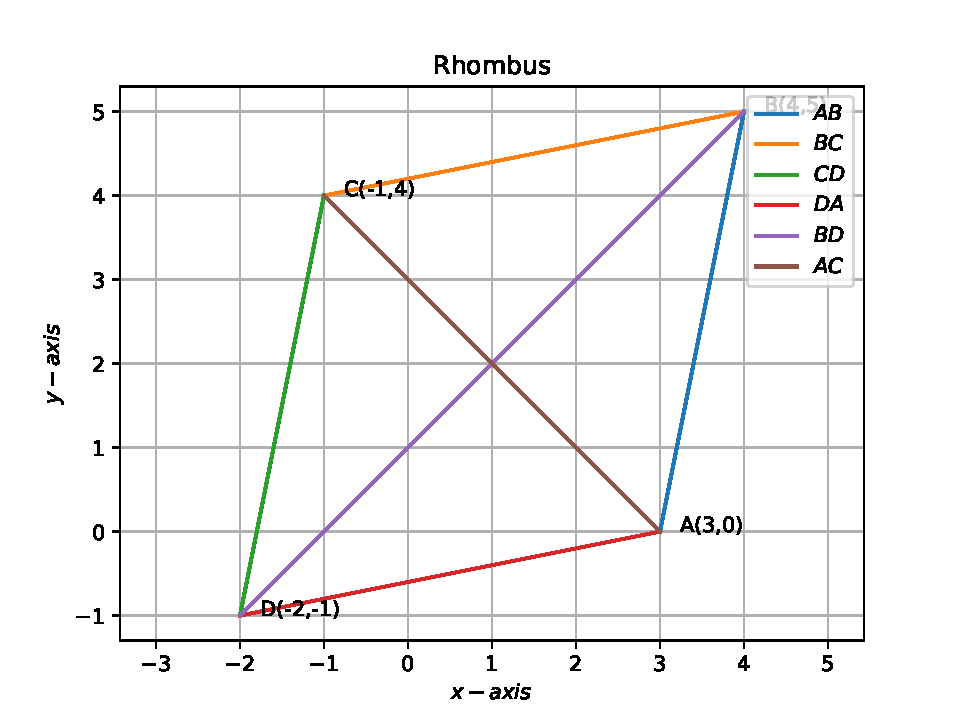
\includegraphics[width=\columnwidth]{chapters/10/7/2/10/figs/fig.pdf}
 \end{center}
\caption{}
\label{fig:chapters/10/7/2/10/gFig1}
\end{figure}


\end{enumerate}


\section{Properties}
\begin{enumerate}[label=\thesection.\arabic*,ref=\thesection.\theenumi]
\item Compute the magnitude of the following vectors:
\begin{align*}
\vec{a}=\hat{i}+\hat{j}+k; \vec{b}=2\hat{i}-7\hat{j}-3\hat{k}; \vec{c}=\frac{1}{\sqrt{3}}\hat{i}+\frac{1}{\sqrt{3}}\hat{j}-\frac{1}{3}\hat{k}
\end{align*}
    \solution 
		\iffalse
\documentclass[12pt]{article}
\usepackage{graphicx}
%\documentclass[journal,12pt,twocolumn]{IEEEtran}
\usepackage[none]{hyphenat}
\usepackage{graphicx}
\usepackage{listings}
\usepackage[english]{babel}
\usepackage{graphicx}
\usepackage{caption} 
\usepackage{hyperref}
\usepackage{booktabs}
\usepackage{commath}
\usepackage{gensymb}
\usepackage{array}
\usepackage{amsmath}   % for having text in math mode
\usepackage{listings}
\lstset{
  frame=single,
  breaklines=true
}
  
%Following 2 lines were added to remove the blank page at the beginning
\usepackage{atbegshi}% http://ctan.org/pkg/atbegshi
\AtBeginDocument{\AtBeginShipoutNext{\AtBeginShipoutDiscard}}
%


%New macro definitions
\newcommand{\mydet}[1]{\ensuremath{\begin{vmatrix}#1\end{vmatrix}}}
\providecommand{\brak}[1]{\ensuremath{\left(#1\right)}}
\providecommand{\norm}[1]{\left\lVert#1\right\rVert}
\newcommand{\solution}{\noindent \textbf{Solution: }}
\newcommand{\myvec}[1]{\ensuremath{\begin{pmatrix}#1\end{pmatrix}}}
\let\vec\mathbf


\begin{document}
\begin{center}
\title{\textbf{Vectors}}
\date{\vspace{-5ex}} %Not to print date automatically
\maketitle
\end{center}
\setcounter{page}{1}
\section*{12$^{th}$ Maths - Exercise 10.2.1}

\begin{enumerate}
\item Compute the magnitude of the following vectors 
$\\ \overrightarrow{a}=\hat{i}+\hat{j}+\hat{k},\overrightarrow{b}=2\hat{i}-7\hat{j}+3\hat{k}$ and $\overrightarrow{c}=\dfrac{1}{\sqrt{3}}\hat{i}+\dfrac{1}{\sqrt{3}}\hat{j}-\dfrac{1}{\sqrt{3}}\hat{k}$.\\
\solution
\fi
Let 
\begin{align}
 \vec{a} = \myvec{1\\1\\1} , \vec{b} = \myvec{2\\ -7 \\ 3},\vec{c} = \myvec{\dfrac{1}{\sqrt{3}}\\ \dfrac{1}{\sqrt{3}} \\ -\dfrac{1}{\sqrt{3}}} 
\label{eq:chapters/12/10/2/1/1}
\end{align}
Then
\begin{align}
	\norm{\vec{a}}&=\sqrt{\vec{a}}^{\top}\vec{a}=\norm{\vec{a}}=\sqrt{3}, 
	\label{eq:chapters/12/10/2/1/3}
	\\ \norm{\vec{b}}&=\sqrt{\vec{b}}^{\top}\vec{b}=\norm{\vec{b}}= \sqrt{62}, 
	\label{eq:chapters/12/10/2/1/4}
	\\ \norm{\vec{c}}&=\sqrt{\vec{c}}^{\top}\vec{c}	=
\norm{\vec{c}}=1
	\label{eq:chapters/12/10/2/1/5}
\end{align}




\item Write two different vectors having same magnitude.
\item Write two different vectors having same direction.
\item Find the values of x and y so that the vectors $2\hat{i}+3\hat{j}$ and $x\hat{i}+y\hat{j}$ are equal.
\item Find the scalar and vector components of the vector with initial point (2, 1) and
terminal point (– 5, 7).
\item Find the sum of the vectors $\vec{a}=\hat{i}-2\hat{j}+\hat{k}$, $\vec{b}=-2\hat{i}+4\hat{j}+5\hat{k}$ and $\vec{c}=\hat{i}-6\hat{j}-7\hat{k}$.
\item Find the unit vector in the direction of the vector $\vec{a}=\hat{i}+\hat{j}+2\hat{k}$.
\item Find the unit vector in the direction of vector $\overrightarrow{PQ}$ , where $\vec{P}$ and $\vec{Q}$ are the points
(1, 2, 3) and (4, 5, 6), respectively.
\item For given vectors, $\vec{a}=2\hat{i}-\hat{j}+2\hat{k}$ and $\vec{b}=-\hat{i}+\hat{j}-\hat{k}$ , find the unit vector in the
direction of the vector $\vec{a}+\vec{b}$.
\\
    \solution 
		\iffalse
\documentclass[journal,12pt,twocolumn]{IEEEtran}
%
\usepackage{setspace}
\usepackage{gensymb}
%\doublespacing
\singlespacing

%\usepackage{graphicx}
%\usepackage{amssymb}
%\usepackage{relsize}
\usepackage[cmex10]{amsmath}
%\usepackage{amsthm}
%\interdisplaylinepenalty=2500
%\savesymbol{iint}
%\usepackage{txfonts}
%\restoresymbol{TXF}{iint}
%\usepackage{wasysym}
\usepackage{amsthm}
%\usepackage{iithtlc}
\usepackage{mathrsfs}
\usepackage{txfonts}
\usepackage{stfloats}
\usepackage{bm}
\usepackage{cite}
\usepackage{cases}
\usepackage{subfig}
%\usepackage{xtab}
\usepackage{longtable}
\usepackage{multirow}
%\usepackage{algorithm}
%\usepackage{algpseudocode}
\usepackage{enumitem}
\usepackage{mathtools}
\usepackage{steinmetz}
\usepackage{tikz}
\usepackage{circuitikz}
\usepackage{verbatim}
\usepackage{tfrupee}
\usepackage[breaklinks=true]{hyperref}
%\usepackage{stmaryrd}
\usepackage{tkz-euclide} % loads  TikZ and tkz-base
%\usetkzobj{all}
\usetikzlibrary{calc,math}
\usepackage{listings}
    \usepackage{color}                                            %%
    \usepackage{array}                                            %%
    \usepackage{longtable}                                        %%
    \usepackage{calc}                                             %%
    \usepackage{multirow}                                         %%
    \usepackage{hhline}                                           %%
    \usepackage{ifthen}                                           %%
  %optionally (for landscape tables embedded in another document): %%
    \usepackage{lscape}     
\usepackage{multicol}
\usepackage{chngcntr}
%\usepackage{enumerate}

%\usepackage{wasysym}
%\newcounter{MYtempeqncnt}
\DeclareMathOperator*{\Res}{Res}
%\renewcommand{\baselinestretch}{2}
\renewcommand\thesection{\arabic{section}}
\renewcommand\thesubsection{\thesection.\arabic{subsection}}
\renewcommand\thesubsubsection{\thesubsection.\arabic{subsubsection}}

\renewcommand\thesectiondis{\arabic{section}}
\renewcommand\thesubsectiondis{\thesectiondis.\arabic{subsection}}
\renewcommand\thesubsubsectiondis{\thesubsectiondis.\arabic{subsubsection}}

% correct bad hyphenation here
\hyphenation{op-tical net-works semi-conduc-tor}
\def\inputGnumericTable{}                                 %%

\lstset{
%language=C,
frame=single, 
breaklines=true,
columns=fullflexible
}
%\lstset{
%language=tex,
%frame=single, 
%breaklines=true
%}

\begin{document}
%


\newtheorem{theorem}{Theorem}[section]
\newtheorem{problem}{Problem}
\newtheorem{proposition}{Proposition}[section]
\newtheorem{lemma}{Lemma}[section]
\newtheorem{corollary}[theorem]{Corollary}
\newtheorem{example}{Example}[section]
\newtheorem{definition}[problem]{Definition}
%\newtheorem{thm}{Theorem}[section] 
%\newtheorem{defn}[thm]{Definition}
%\newtheorem{algorithm}{Algorithm}[section]
%\newtheorem{cor}{Corollary}
\newcommand{\BEQA}{\begin{eqnarray}}
\newcommand{\EEQA}{\end{eqnarray}}
\newcommand{\define}{\stackrel{\triangle}{=}}

\bibliographystyle{IEEEtran}
%\bibliographystyle{ieeetr}


\providecommand{\mbf}{\mathbf}
\providecommand{\pr}[1]{\ensuremath{\Pr\left(#1\right)}}
\providecommand{\qfunc}[1]{\ensuremath{Q\left(#1\right)}}
\providecommand{\sbrak}[1]{\ensuremath{{}\left[#1\right]}}
\providecommand{\lsbrak}[1]{\ensuremath{{}\left[#1\right.}}
\providecommand{\rsbrak}[1]{\ensuremath{{}\left.#1\right]}}
\providecommand{\brak}[1]{\ensuremath{\left(#1\right)}}
\providecommand{\lbrak}[1]{\ensuremath{\left(#1\right.}}
\providecommand{\rbrak}[1]{\ensuremath{\left.#1\right)}}
\providecommand{\cbrak}[1]{\ensuremath{\left\{#1\right\}}}
\providecommand{\lcbrak}[1]{\ensuremath{\left\{#1\right.}}
\providecommand{\rcbrak}[1]{\ensuremath{\left.#1\right\}}}
\theoremstyle{remark}
\newtheorem{rem}{Remark}
\newcommand{\sgn}{\mathop{\mathrm{sgn}}}
\providecommand{\abs}[1]{\left\vert#1\right\vert}
\providecommand{\res}[1]{\Res\displaylimits_{#1}} 
\providecommand{\norm}[1]{\left\lVert#1\right\rVert}
%\providecommand{\norm}[1]{\lVert#1\rVert}
\providecommand{\mtx}[1]{\mathbf{#1}}
\providecommand{\mean}[1]{E\left[ #1 \right]}
\providecommand{\fourier}{\overset{\mathcal{F}}{ \rightleftharpoons}}
%\providecommand{\hilbert}{\overset{\mathcal{H}}{ \rightleftharpoons}}
\providecommand{\system}{\overset{\mathcal{H}}{ \longleftrightarrow}}
	%\newcommand{\solution}[2]{\textbf{Solution:}{#1}}
\newcommand{\solution}{\noindent \textbf{Solution: }}
\newcommand{\cosec}{\,\text{cosec}\,}
\providecommand{\dec}[2]{\ensuremath{\overset{#1}{\underset{#2}{\gtrless}}}}
\newcommand{\myvec}[1]{\ensuremath{\begin{pmatrix}#1\end{pmatrix}}}
\newcommand{\mydet}[1]{\ensuremath{\begin{vmatrix}#1\end{vmatrix}}}
%\numberwithin{equation}{section}
\numberwithin{equation}{subsection}
%\numberwithin{problem}{section}
%\numberwithin{definition}{section}
\makeatletter
\@addtoreset{figure}{problem}
\makeatother

\let\StandardTheFigure\thefigure
\let\vec\mathbf
%\renewcommand{\thefigure}{\theproblem.\arabic{figure}}
\renewcommand{\thefigure}{\theproblem}
%\setlist[enumerate,1]{before=\renewcommand\theequation{\theenumi.\arabic{equation}}
%\counterwithin{equation}{enumi}


%\renewcommand{\theequation}{\arabic{subsection}.\arabic{equation}}

\def\putbox#1#2#3{\makebox[0in][l]{\makebox[#1][l]{}\raisebox{\baselineskip}[0in][0in]{\raisebox{#2}[0in][0in]{#3}}}}
     \def\rightbox#1{\makebox[0in][r]{#1}}
     \def\centbox#1{\makebox[0in]{#1}}
     \def\topbox#1{\raisebox{-\baselineskip}[0in][0in]{#1}}
     \def\midbox#1{\raisebox{-0.5\baselineskip}[0in][0in]{#1}}

\vspace{3cm}


\title{EE2802: Assignment5}
\author{Nikam Pratik Balasaheb (EE21BTECH11037)}





% make the title area
\maketitle

\newpage

%\tableofcontents

\bigskip

\renewcommand{\thefigure}{\theenumi}
\renewcommand{\thetable}{\theenumi}
%\renewcommand{\theequation}{\theenumi}

\section{Problem}
For the vectors $ \vec a = \myvec{ 2\\-1\\2 } \text{ and } \vec b = \myvec{ -1\\1\\-1 }$, find the unit vector along the direction of $ \vec a + \vec b$.

\section{Solution}
\fi
Since
\begin{align}
\vec a + \vec b = \vec u = \myvec{ 2\\-1\\2 } + \myvec{ -1\\1\\-1 }
= \myvec{ 1\\0\\1 }
\end{align}
the unit vector in direction of $\vec u$ is,
\begin{align}
 \hat{\vec{u}} &= \frac{\vec u}{\norm{ \vec{u} }}
 = \frac{1}{\sqrt{2}} \vec u \\
\implies \hat{\vec{u}} &= \frac{1}{\sqrt{2}} \myvec{ 1\\0\\1 } 
\end{align}





\item Find a vector in the direction of vector $5\hat{i}-\hat{j}+2\hat{k}$ which has magnitude 8 units.
    has magnitude 8 units.
   \\ 
    \solution 
		\iffalse
\documentclass[journal,12pt,twocolumn]{IEEEtran}
\usepackage{setspace}
\usepackage{gensymb}
\usepackage{xcolor}
\usepackage{caption}
\singlespacing
\usepackage{siunitx}
\usepackage[cmex10]{amsmath}
\usepackage{mathtools}
\usepackage{hyperref}
\usepackage{amsthm}
\usepackage{mathrsfs}
\usepackage{txfonts}
\usepackage{stfloats}
\usepackage{cite}
\usepackage{cases}
\usepackage{subfig}
\usepackage{longtable}
\usepackage{multirow}
\usepackage{enumitem}
\usepackage{mathtools}
\usepackage{listings}
\usepackage{tikz}
\usetikzlibrary{shapes,arrows,positioning}
\usepackage{circuitikz}
\let\vec\mathbf
\DeclareMathOperator*{\Res}{Res}
\renewcommand\thesection{\arabic{section}}
\renewcommand\thesubsection{\thesection.\arabic{subsection}}
\renewcommand\thesubsubsection{\thesubsection.\arabic{subsubsection}}

\renewcommand\thesectiondis{\arabic{section}}
\renewcommand\thesubsectiondis{\thesectiondis.\arabic{subsection}}
\renewcommand\thesubsubsectiondis{\thesubsectiondis.\arabic{subsubsection}}
\hyphenation{op-tical net-works semi-conduc-tor}

\lstset{
language=Python,
frame=single, 
breaklines=true,
columns=fullflexible
}
\begin{document}
\theoremstyle{definition}
\newtheorem{theorem}{Theorem}[section]
\newtheorem{problem}{Problem}
\newtheorem{proposition}{Proposition}[section]
\newtheorem{lemma}{Lemma}[section]
\newtheorem{corollary}[theorem]{Corollary}
\newtheorem{example}{Example}[section]
\newtheorem{definition}{Definition}[section]
\newcommand{\BEQA}{\begin{eqnarray}}
\newcommand{\EEQA}{\end{eqnarray}}
\newcommand{\define}{\stackrel{\triangle}{=}}
\newcommand{\myvec}[1]{\ensuremath{\begin{pmatrix}#1\end{pmatrix}}}
\newcommand{\mydet}[1]{\ensuremath{\begin{vmatrix}#1\end{vmatrix}}}

\bibliographystyle{IEEEtran}
\providecommand{\nCr}[2]{\,^{#1}C_{#2}} % nCr
\providecommand{\nPr}[2]{\,^{#1}P_{#2}} % nPr
\providecommand{\mbf}{\mathbf}
\providecommand{\pr}[1]{\ensuremath{\Pr\left(#1\right)}}
\providecommand{\qfunc}[1]{\ensuremath{Q\left(#1\right)}}
\providecommand{\sbrak}[1]{\ensuremath{{}\left[#1\right]}}
\providecommand{\lsbrak}[1]{\ensuremath{{}\left[#1\right.}}
\providecommand{\rsbrak}[1]{\ensuremath{{}\left.#1\right]}}
\providecommand{\brak}[1]{\ensuremath{\left(#1\right)}}
\providecommand{\lbrak}[1]{\ensuremath{\left(#1\right.}}
\providecommand{\rbrak}[1]{\ensuremath{\left.#1\right)}}
\providecommand{\cbrak}[1]{\ensuremath{\left\{#1\right\}}}
\providecommand{\lcbrak}[1]{\ensuremath{\left\{#1\right.}}
\providecommand{\rcbrak}[1]{\ensuremath{\left.#1\right\}}}
\theoremstyle{remark}
\newtheorem{rem}{Remark}
\newcommand{\sgn}{\mathop{\mathrm{sgn}}}
\newcommand{\rect}{\mathop{\mathrm{rect}}}
\newcommand{\sinc}{\mathop{\mathrm{sinc}}}
\providecommand{\abs}[1]{\left\vert#1\right\vert}
\providecommand{\res}[1]{\Res\displaylimits_{#1}} 
\providecommand{\norm}[1]{\left\Vert#1\right\Vert}
\providecommand{\mtx}[1]{\mathbf{#1}}
\providecommand{\mean}[1]{E\left[ #1 \right]}
\providecommand{\fourier}{\overset{\mathcal{F}}{ \rightleftharpoons}}
\providecommand{\ztrans}{\overset{\mathcal{Z}}{ \rightleftharpoons}}
\providecommand{\system}[1]{\overset{\mathcal{#1}}{ \longleftrightarrow}}
\newcommand{\solution}{\noindent \textbf{Solution: }}
\providecommand{\dec}[2]{\ensuremath{\overset{#1}{\underset{#2}{\gtrless}}}}
\let\StandardTheFigure\thefigure
\def\putbox#1#2#3{\makebox[0in][l]{\makebox[#1][l]{}\raisebox{\baselineskip}[0in][0in]{\raisebox{#2}[0in][0in]{#3}}}}
     \def\rightbox#1{\makebox[0in][r]{#1}}
     \def\centbox#1{\makebox[0in]{#1}}
     \def\topbox#1{\raisebox{-\baselineskip}[0in][0in]{#1}}
     \def\midbox#1{\raisebox{-0.5\baselineskip}[0in][0in]{#1}}

\vspace{3cm}
\title{Straight Lines Assignment}
\author{Gautam Singh}
\maketitle
\bigskip

\begin{abstract}
    This document contains the solution to Question 10 of Exercise 2 in Chapter
    10 of the class 12 NCERT textbook.
\end{abstract}

\begin{enumerate}
		\fi
Let the required vector be $c\myvec{5\\-1\\2}$, where $c\in\mathbb{R}$.
    Since this vector has magnitude 8,
    \begin{align}
        \norm{c\myvec{5\\-1\\2\\}} = c\sqrt{5^2+\brak{-1}^2+2^2} &= 8 \\
        \implies c = \frac{8}{\sqrt{30}} &= \frac{4\sqrt{30}}{15}
        \label{eq:12/10/2/10const}
    \end{align}
    Thus, the required vector is $\frac{4\sqrt{30}}{15}\myvec{5\\-1\\2}$.


\item Show that the vectors $2\hat{i}-3\hat{j}+4\hat{k}$ and $-4\hat{i}+6\hat{j}-8\hat{k}$ are collinear.
   \\ 
    \solution 
		\iffalse
\documentclass[12pt]{article}
\usepackage{graphicx}
\graphicspath{{./figs/}}{}
\usepackage{amsmath,amssymb,amsfonts,amsthm}
\newcommand{\myvec}[1]{\ensuremath{\begin{pmatrix}#1\end{pmatrix}}}
\providecommand{\norm}[1]{\lVert#1\rVert}
\usepackage{listings}
\usepackage{watermark}
\usepackage{titlesec}
\usepackage{caption}
\usepackage{extarrows}
\let\vec\mathbf
\lstset{
frame=single, 
breaklines=true,
columns=fullflexible
}
\thiswatermark{\centering \put(0,-105.0){
\includegraphics[scale=0.15]{/sdcard/IITH/vectors/12.10.2.11/figs/logo.png}} }
\title{\mytitle}
\title{
Assignment - 12.10.2.11
}
\author{Surajit Sarkar}
\begin{document}
\maketitle
\tableofcontents
\bigskip
\section{\textbf{Problem}}
Show that the vectors $2\hat{i}+3\hat{j}+4\hat{k}$ and $-4\hat{i}+6\hat{j}-8\hat{k}$ are collinear.
\section{\textbf{Solution}}
\fi
Let
\begin{align}
\vec{A}=\myvec{2\\3\\4},\vec{B}=\myvec{-4\\6\\-8}\\
 \end{align}
 Forming the collinearity matrix
 \begin{align}        
\myvec{\vec{A}^{\top}\\ \vec{B}^{\top}}=\myvec{2&-3&4\\-4&6&-8}
 \xleftrightarrow{\frac{1}{2}R_1\to R_1}\myvec{1&-\frac{3}{2}&2\\-4&6&-8}\\
\xleftrightarrow{-\frac{1}{4}R_2\leftarrow R_2}\myvec{1&-\frac{3}{2}&2\\1&\frac{3}{2}&2}
\xleftrightarrow{R_2-1R_1\to R_2}\myvec{1&-\frac{3}{2}&2\\0&0&0}
\end{align}
Thus, the rank of the matrix is 1 and the vectors are collinear.

\item Find the direction cosines of the vector $\hat{i}+2\hat{j}+3\hat{k}$.
	\\
    \solution 
		\iffalse
\documentclass[12pt]{article}
\usepackage{graphicx}
%\documentclass[journal,12pt,twocolumn]{IEEEtran}
\usepackage[none]{hyphenat}
\usepackage{graphicx}
\usepackage{listings}
\usepackage[english]{babel}
\usepackage{graphicx}
\usepackage{caption}
\usepackage[parfill]{parskip}
\usepackage{hyperref}
\usepackage{booktabs}
%\usepackage{setspace}\doublespacing\pagestyle{plain}
\def\inputGnumericTable{}
\usepackage{color}                                            %%
    \usepackage{array}                                            %%
    \usepackage{longtable}                                        %%
    \usepackage{calc}                                             %%
    \usepackage{multirow}                                         %%
    \usepackage{hhline}                                           %%
    \usepackage{ifthen}
\usepackage{array}
\usepackage{amsmath}   % for having text in math mode
\usepackage{parallel,enumitem}
\usepackage{listings}
\lstset{
language=tex,
frame=single,
breaklines=true
}
 
%Following 2 lines were added to remove the blank page at the beginning
\usepackage{atbegshi}% http://ctan.org/pkg/atbegshi
\AtBeginDocument{\AtBeginShipoutNext{\AtBeginShipoutDiscard}}
%
%New macro definitions
\newcommand{\mydet}[1]{\ensuremath{\begin{vmatrix}#1\end{vmatrix}}}
\providecommand{\brak}[1]{\ensuremath{\left(#1\right)}}
\providecommand{\norm}[1]{\left\lVert#1\right\rVert}
\newcommand{\solution}{\noindent \textbf{Solution: }}
\newcommand{\myvec}[1]{\ensuremath{\begin{pmatrix}#1\end{pmatrix}}}
\let\vec\mathbf
\begin{document}
\begin{center}
\enlargethispage{-4cm}
\title{\textbf{Straight Lines}}
\date{\vspace{-5ex}} %Not to print date automatically
\maketitle
\end{center}
\setcounter{page}{1}
\section*{12$^{th}$ Maths - Chapter 10}
This is Problem-12 from Exercise 10.2
\begin{enumerate}
\item Find the direction cosines of the vector $\hat{i} +2\hat{j}+3\hat{k}$.

\solution 
		The direction cosines are the cosines of the angles formed by the given vector with the respective axes, let $\vec{A}$ be the given vector
\fi
Let
\begin{align}
	\vec{A} =\myvec{1\\2\\3}
\end{align}
The Directional vectors of $x,y$ and $z$ axes are given respectively as
\begin{align}
		\vec{e_1} =\myvec{1\\0\\0},\vec{e_2}=\myvec{0\\1\\0},\vec{e_3} =\myvec{0\\0\\1}
\end{align}
		The magnitudes for $\vec{A}$ and directional vectors $\vec{e_1},\vec{e_2},\vec{e_3}$ are
	\begin{align}
\norm{\vec{A}} =\sqrt{14},\norm{\vec{e_1}}=1,\norm{\vec{e_1}}=1,\norm{\vec{e_1}}=1
	\end{align}
	\iffalse
Let 
\begin{align}
	\cos\theta_i=1,2,3  
\end{align}
\fi
		So for different values of $\cos\theta_i$ the direction cosines of vector $\vec{A}$ are
\begin{align}
	\cos\theta_1 &=\frac{\myvec{1&2&3}\myvec{1\\0\\0}}{\sqrt{14}}=\frac{1}{\sqrt{14}}\\
	\cos\theta_2 &=\frac{\myvec{1&2&3}\myvec{0\\1\\0}}{\sqrt{14}}=\frac{2}{\sqrt{14}}\\
	\cos\theta_3 &=\frac{\myvec{1&2&3}\myvec{0\\0\\1}}{\sqrt{14}}=\frac{3}{\sqrt{14}}
\end{align}

\item Find the direction cosines of the vector joining the points $\vec{A}$ (1, 2, –3) and
$\vec{B}$(–1, –2, 1), directed from $\vec{A}$ to $\vec{B}$.
	\\
    \solution 
		\iffalse
\documentclass[12pt]{article}
\usepackage{graphicx}
%\documentclass[journal,12pt,twocolumn]{IEEEtran}
\usepackage[none]{hyphenat}
\usepackage{graphicx}
\usepackage{listings}
\usepackage[english]{babel}
\usepackage{graphicx}
\usepackage{caption}
\usepackage[parfill]{parskip}
\usepackage{hyperref}
\usepackage{booktabs}
%\usepackage{setspace}\doublespacing\pagestyle{plain}
\def\inputGnumericTable{}
\usepackage{color}                                            %%
    \usepackage{array}                                            %%
    \usepackage{longtable}                                        %%
    \usepackage{calc}                                             %%
    \usepackage{multirow}                                         %%
    \usepackage{hhline}                                           %%
    \usepackage{ifthen}
\usepackage{array}
\usepackage{amsmath}   % for having text in math mode
\usepackage{parallel,enumitem}
\usepackage{listings}
\lstset{
language=tex,
frame=single,
breaklines=true
}
 
%Following 2 lines were added to remove the blank page at the beginning
\usepackage{atbegshi}% http://ctan.org/pkg/atbegshi
\AtBeginDocument{\AtBeginShipoutNext{\AtBeginShipoutDiscard}}
%
%New macro definitions
\newcommand{\mydet}[1]{\ensuremath{\begin{vmatrix}#1\end{vmatrix}}}
\providecommand{\brak}[1]{\ensuremath{\left(#1\right)}}
\providecommand{\norm}[1]{\left\lVert#1\right\rVert}
\newcommand{\solution}{\noindent \textbf{Solution: }}
\newcommand{\myvec}[1]{\ensuremath{\begin{pmatrix}#1\end{pmatrix}}}
\let\vec\mathbf
\begin{document}
\begin{center}
\enlargethispage{-4cm}
\title{\textbf{Vector Algebra}}
\date{\vspace{-5ex}} %Not to print date automatically
\maketitle
\end{center}
\setcounter{page}{1}
\section*{12$^{th}$ Maths - Chapter 10}
 Exercise 10.2 Problem-13
\begin{enumerate}
\item Find the direction cosines of the vector joining the points A (1, 2, –3) and
B(–1, –2, 1), directed from A to B.

\solution 
\fi
The direction vector  is given by 
\begin{align}
	\vec{m}= \myvec{-1\\-2\\1}-\myvec{1\\2\\-3}=\myvec{-2\\-4\\4}
\end{align}
and the corresponding unit vector is
\begin{align}
	\frac{\vec{m}}{\norm{\vec{m}}}=\frac{1}{6}{\myvec{-2\\-4\\4}}
\end{align}

\item Show that the vector $\hat{i}+\hat{j}+\hat{k}$ is equally inclined to the axes OX, OY and OZ.
	\\
\solution
		\iffalse
\documentclass[12pt]{article}
\usepackage{graphicx}
%\documentclass[journal,12pt,twocolumn]{IEEEtran}
\usepackage[none]{hyphenat}
\usepackage{graphicx}
\usepackage{listings}
\usepackage[english]{babel}
\usepackage{graphicx}
\usepackage{caption} 
\usepackage{hyperref}
\usepackage{booktabs}
\usepackage{commath}
\usepackage{gensymb}
\usepackage{array}
\usepackage{amsmath}   % for having text in math mode
\usepackage{listings}
\lstset{
  frame=single,
  breaklines=true
}
  
%Following 2 lines were added to remove the blank page at the beginning
\usepackage{atbegshi}% http://ctan.org/pkg/atbegshi
\AtBeginDocument{\AtBeginShipoutNext{\AtBeginShipoutDiscard}}
%


%New macro definitions
\newcommand{\mydet}[1]{\ensuremath{\begin{vmatrix}#1\end{vmatrix}}}
\providecommand{\brak}[1]{\ensuremath{\left(#1\right)}}
\providecommand{\norm}[1]{\left\lVert#1\right\rVert}
\newcommand{\solution}{\noindent \textbf{Solution: }}
\newcommand{\myvec}[1]{\ensuremath{\begin{pmatrix}#1\end{pmatrix}}}
\let\vec\mathbf


\begin{document}
\begin{center}
\title{\textbf{Vector Algebra}}
\date{\vspace{-5ex}} %Not to print date automatically
\maketitle
\end{center}
\setcounter{page}{1}
\section{12$^{th}$ Maths - Exercise 10.2.14}

\begin{enumerate}
\item Show that the vector $\hat{i}+\hat{j}+\hat{k}$ is equally inclined to the axes OX, OY, and OZ
\section{Solution}
\fi
Let
\begin{align}
 \vec{A} = \myvec{1\\1\\1}
\end{align}
Since all entries of the vector are equal, the vector is equally inclined to the axes.

\item Find the position vector of a point R which divides the line joining two points $\vec{P}$
and $\vec{Q}$ whose position vectors are $\hat{i}+2\hat{j}-\hat{k}$ and $-\hat{i}+\hat{j}+\hat{k}$ respectively, in the
ratio 2 : 1
\begin{enumerate}
    \item  internally
    \item  externally
\end{enumerate}
\solution
		\iffalse
\documentclass[journal,12pt,twocolumn]{IEEEtran}
%
\usepackage{setspace}
\usepackage{gensymb}
%\doublespacing
\singlespacing

%\usepackage{graphicx}
%\usepackage{amssymb}
%\usepackage{relsize}
\usepackage[cmex10]{amsmath}
%\usepackage{amsthm}
%\interdisplaylinepenalty=2500
%\savesymbol{iint}
%\usepackage{txfonts}
%\restoresymbol{TXF}{iint}
%\usepackage{wasysym}
\usepackage{amsthm}
%\usepackage{iithtlc}
\usepackage{mathrsfs}
\usepackage{txfonts}
\usepackage{stfloats}
\usepackage{bm}
\usepackage{cite}
\usepackage{cases}
\usepackage{subfig}
%\usepackage{xtab}
\usepackage{longtable}
\usepackage{multirow}
%\usepackage{algorithm}
%\usepackage{algpseudocode}
\usepackage{enumitem}
\usepackage{mathtools}
\usepackage{steinmetz}
\usepackage{tikz}
\usepackage{circuitikz}
\usepackage{verbatim}
\usepackage{tfrupee}
\usepackage[breaklinks=true]{hyperref}
%\usepackage{stmaryrd}
\usepackage{tkz-euclide} % loads  TikZ and tkz-base
%\usetkzobj{all}
\usetikzlibrary{calc,math}
\usepackage{listings}
    \usepackage{color}                                            %%
    \usepackage{array}                                            %%
    \usepackage{longtable}                                        %%
    \usepackage{calc}                                             %%
    \usepackage{multirow}                                         %%
    \usepackage{hhline}                                           %%
    \usepackage{ifthen}                                           %%
  %optionally (for landscape tables embedded in another document): %%
    \usepackage{lscape}     
\usepackage{multicol}
\usepackage{chngcntr}
%\usepackage{enumerate}
\usepackage{graphicx}

%\usepackage{wasysym}
%\newcounter{MYtempeqncnt}
\DeclareMathOperator*{\Res}{Res}
%\renewcommand{\baselinestretch}{2}
\renewcommand\thesection{\arabic{section}}
\renewcommand\thesubsection{\thesection.\arabic{subsection}}
\renewcommand\thesubsubsection{\thesubsection.\arabic{subsubsection}}

\renewcommand\thesectiondis{\arabic{section}}
\renewcommand\thesubsectiondis{\thesectiondis.\arabic{subsection}}
\renewcommand\thesubsubsectiondis{\thesubsectiondis.\arabic{subsubsection}}

% correct bad hyphenation here
\hyphenation{op-tical net-works semi-conduc-tor}
\def\inputGnumericTable{}                                 %%

\lstset{
%language=C,
frame=single, 
breaklines=true,
columns=fullflexible
}
%\lstset{
%language=tex,
%frame=single, 
%breaklines=true
%}

\begin{document}
%


\newtheorem{theorem}{Theorem}[section]
\newtheorem{problem}{Problem}
\newtheorem{proposition}{Proposition}[section]
\newtheorem{lemma}{Lemma}[section]
\newtheorem{corollary}[theorem]{Corollary}
\newtheorem{example}{Example}[section]
\newtheorem{definition}[problem]{Definition}
%\newtheorem{thm}{Theorem}[section] 
%\newtheorem{defn}[thm]{Definition}
%\newtheorem{algorithm}{Algorithm}[section]
%\newtheorem{cor}{Corollary}
\newcommand{\BEQA}{\begin{eqnarray}}
\newcommand{\EEQA}{\end{eqnarray}}
\newcommand{\define}{\stackrel{\triangle}{=}}

\bibliographystyle{IEEEtran}
%\bibliographystyle{ieeetr}


\providecommand{\mbf}{\mathbf}
\providecommand{\pr}[1]{\ensuremath{\Pr\left(#1\right)}}
\providecommand{\qfunc}[1]{\ensuremath{Q\left(#1\right)}}
\providecommand{\sbrak}[1]{\ensuremath{{}\left[#1\right]}}
\providecommand{\lsbrak}[1]{\ensuremath{{}\left[#1\right.}}
\providecommand{\rsbrak}[1]{\ensuremath{{}\left.#1\right]}}
\providecommand{\brak}[1]{\ensuremath{\left(#1\right)}}
\providecommand{\lbrak}[1]{\ensuremath{\left(#1\right.}}
\providecommand{\rbrak}[1]{\ensuremath{\left.#1\right)}}
\providecommand{\cbrak}[1]{\ensuremath{\left\{#1\right\}}}
\providecommand{\lcbrak}[1]{\ensuremath{\left\{#1\right.}}
\providecommand{\rcbrak}[1]{\ensuremath{\left.#1\right\}}}
\theoremstyle{remark}
\newtheorem{rem}{Remark}
\newcommand{\sgn}{\mathop{\mathrm{sgn}}}
\providecommand{\abs}[1]{\left\vert#1\right\vert}
\providecommand{\res}[1]{\Res\displaylimits_{#1}} 
\providecommand{\norm}[1]{\left\lVert#1\right\rVert}
%\providecommand{\norm}[1]{\lVert#1\rVert}
\providecommand{\mtx}[1]{\mathbf{#1}}
\providecommand{\mean}[1]{E\left[ #1 \right]}
\providecommand{\fourier}{\overset{\mathcal{F}}{ \rightleftharpoons}}
%\providecommand{\hilbert}{\overset{\mathcal{H}}{ \rightleftharpoons}}
\providecommand{\system}{\overset{\mathcal{H}}{ \longleftrightarrow}}
	%\newcommand{\solution}[2]{\textbf{Solution:}{#1}}
\newcommand{\solution}{\noindent \textbf{Solution: }}
\newcommand{\cosec}{\,\text{cosec}\,}
\providecommand{\dec}[2]{\ensuremath{\overset{#1}{\underset{#2}{\gtrless}}}}
\newcommand{\myvec}[1]{\ensuremath{\begin{pmatrix}#1\end{pmatrix}}}
\newcommand{\mydet}[1]{\ensuremath{\begin{vmatrix}#1\end{vmatrix}}}
%\numberwithin{equation}{section}
\numberwithin{equation}{subsection}
%\numberwithin{problem}{section}
%\numberwithin{definition}{section}
\makeatletter
\@addtoreset{figure}{problem}
\makeatother

\let\StandardTheFigure\thefigure
\let\vec\mathbf
%\renewcommand{\thefigure}{\theproblem.\arabic{figure}}
\renewcommand{\thefigure}{\theproblem}
%\setlist[enumerate,1]{before=\renewcommand\theequation{\theenumi.\arabic{equation}}
%\counterwithin{equation}{enumi}


%\renewcommand{\theequation}{\arabic{subsection}.\arabic{equation}}

\def\putbox#1#2#3{\makebox[0in][l]{\makebox[#1][l]{}\raisebox{\baselineskip}[0in][0in]{\raisebox{#2}[0in][0in]{#3}}}}
     \def\rightbox#1{\makebox[0in][r]{#1}}
     \def\centbox#1{\makebox[0in]{#1}}
     \def\topbox#1{\raisebox{-\baselineskip}[0in][0in]{#1}}
     \def\midbox#1{\raisebox{-0.5\baselineskip}[0in][0in]{#1}}

\vspace{3cm}

\title{EE2802: Assignment2}
\author{Nikam Pratik Balasaheb}





% make the title area
\maketitle

\newpage

%\tableofcontents

\bigskip

\renewcommand{\thefigure}{\theenumi}
\renewcommand{\thetable}{\theenumi}
%\renewcommand{\theequation}{\theenumi}

\section{Problem}
Find the position vector of a point R which divides the line joining two points P = $\myvec{1\\ 2 \\-1}$ and Q = $\myvec{ -1\\1\\1 }$ in the ratio 2:1 
\begin{enumerate}
\item internally
\item externally
\end{enumerate}

\section{Solution}

\begin{align}
\vec{P} = \myvec{ 1\\2\\-1} \\
 \vec{Q} = \myvec{ -1\\1\\1}
\end{align}

\fi

\begin{enumerate}


\item When $\vec{R}$ divides line segment joining $\vec{P}$ and $\vec{Q}$ internally,
\begin{align}
\vec{R} &= \frac{2 \vec{P} + 1 \vec{Q}}{3} \\
 &= \frac{2}{3} \vec{P} + \frac{1}{3} \vec{Q}\\
\vec{R} &= \myvec{\frac{1}{3}\\[1pt] \frac{5}{3} \\[1pt] \frac{-1}{3}}
\end{align}

\item When $\vec{R}$ divides line segment joining $\vec{P}$ and $\vec{Q}$ externally,
\begin{align}
\vec{R} &= 2 \vec{Q} - \vec{P} \\
 &= 2 \myvec{ -1\\1\\1} - \myvec{ 1\\2\\-1}\\
\vec{R} &= \myvec{ -3\\ 0 \\ 3 }
\end{align}


\end{enumerate}
See Fig. 
\ref{fig:chapters/12/10/2/15/}.
\begin{figure}[!ht]
\centering
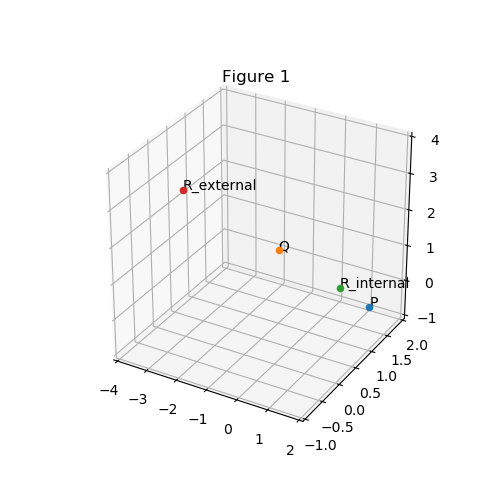
\includegraphics[width=\columnwidth]{chapters/12/10/2/15/figs/Figure_1.png}
\caption{}
\label{fig:chapters/12/10/2/15/}
\end{figure}



\item Find the position vector of the mid point of the vector joining the points $\vec{P}$(2, 3, 4)
and $\vec{Q}$(4, 1, –2).
\\
\solution
		\iffalse
\documentclass[A4,12pt,twocolumn]{IEEEtran}
%
\usepackage{setspace}
\usepackage{gensymb}
%\doublespacing
\singlespacing

%\usepackage{graphicx}
%\usepackage{amssymb}
%\usepackage{relsize}
\usepackage[cmex10]{amsmath}
%\usepackage{amsthm}
%\interdisplaylinepenalty=2500
%\savesymbol{iint}
%\usepackage{txfonts}
%\restoresymbol{TXF}{iint}
%\usepackage{wasysym}
\usepackage{amsthm}
%\usepackage{iithtlc}
\usepackage{mathrsfs}
\usepackage{txfonts}
\usepackage{stfloats}
\usepackage{bm}
\usepackage{cite}
\usepackage{cases}
\usepackage{subfig}
%\usepackage{xtab}
\usepackage{longtable}
\usepackage{multirow}
%\usepackage{algorithm}
%\usepackage{algpseudocode}
\usepackage{enumitem}
\usepackage{mathtools}
\usepackage{steinmetz}
\usepackage{tikz}
\usepackage{circuitikz}
\usepackage{verbatim}
\usepackage{tfrupee}
\usepackage[breaklinks=true]{hyperref}
%\usepackage{stmaryrd}
\usepackage{tkz-euclide} % loads  TikZ and tkz-base
%\usetkzobj{all}
\usetikzlibrary{calc,math}
\usepackage{listings}
    \usepackage{color}                                            %%
    \usepackage{array}                                            %%
    \usepackage{longtable}                                        %%
    \usepackage{calc}                                             %%
    \usepackage{multirow}                                         %%
    \usepackage{hhline}                                           %%
    \usepackage{ifthen}                                           %%
  %optionally (for landscape tables embedded in another document): %%
    \usepackage{lscape}     
\usepackage{multicol}
\usepackage{chngcntr}
%\usepackage{enumerate}

%\usepackage{wasysym}
%\newcounter{MYtempeqncnt}
\DeclareMathOperator*{\Res}{Res}
%\renewcommand{\baselinestretch}{2}
\renewcommand\thesection{\arabic{section}}
\renewcommand\thesubsection{\thesection.\arabic{subsection}}
\renewcommand\thesubsubsection{\thesubsection.\arabic{subsubsection}}

\renewcommand\thesectiondis{\arabic{section}}
\renewcommand\thesubsectiondis{\thesectiondis.\arabic{subsection}}
\renewcommand\thesubsubsectiondis{\thesubsectiondis.\arabic{subsubsection}}

% correct bad hyphenation here
\hyphenation{op-tical net-works semi-conduc-tor}
\def\inputGnumericTable{}                                 %%

\lstset{
%language=C,
frame=single, 
breaklines=true,
columns=fullflexible
}
%\lstset{
%language=tex,
%frame=single, 
%breaklines=true
%}

\begin{document}
%


\newtheorem{theorem}{Theorem}[section]
\newtheorem{problem}{Problem}
\newtheorem{proposition}{Proposition}[section]
\newtheorem{lemma}{Lemma}[section]
\newtheorem{corollary}[theorem]{Corollary}
\newtheorem{example}{Example}[section]
\newtheorem{definition}[problem]{Definition}
%\newtheorem{thm}{Theorem}[section] 
%\newtheorem{defn}[thm]{Definition}
%\newtheorem{algorithm}{Algorithm}[section]
%\newtheorem{cor}{Corollary}
\newcommand{\BEQA}{\begin{eqnarray}}
\newcommand{\EEQA}{\end{eqnarray}}
\newcommand{\define}{\stackrel{\triangle}{=}}

\bibliographystyle{IEEEtran}
%\bibliographystyle{ieeetr}


\providecommand{\mbf}{\mathbf}
\providecommand{\pr}[1]{\ensuremath{\Pr\left(#1\right)}}
\providecommand{\qfunc}[1]{\ensuremath{Q\left(#1\right)}}
\providecommand{\sbrak}[1]{\ensuremath{{}\left[#1\right]}}
\providecommand{\lsbrak}[1]{\ensuremath{{}\left[#1\right.}}
\providecommand{\rsbrak}[1]{\ensuremath{{}\left.#1\right]}}
\providecommand{\brak}[1]{\ensuremath{\left(#1\right)}}
\providecommand{\lbrak}[1]{\ensuremath{\left(#1\right.}}
\providecommand{\rbrak}[1]{\ensuremath{\left.#1\right)}}
\providecommand{\cbrak}[1]{\ensuremath{\left\{#1\right\}}}
\providecommand{\lcbrak}[1]{\ensuremath{\left\{#1\right.}}
\providecommand{\rcbrak}[1]{\ensuremath{\left.#1\right\}}}
\theoremstyle{remark}
\newtheorem{rem}{Remark}
\newcommand{\sgn}{\mathop{\mathrm{sgn}}}
\providecommand{\abs}[1]{\left\vert#1\right\vert}
\providecommand{\res}[1]{\Res\displaylimits_{#1}} 
\providecommand{\norm}[1]{\left\lVert#1\right\rVert}
%\providecommand{\norm}[1]{\lVert#1\rVert}
\providecommand{\mtx}[1]{\mathbf{#1}}
\providecommand{\mean}[1]{E\left[ #1 \right]}
\providecommand{\fourier}{\overset{\mathcal{F}}{ \rightleftharpoons}}
%\providecommand{\hilbert}{\overset{\mathcal{H}}{ \rightleftharpoons}}
\providecommand{\system}{\overset{\mathcal{H}}{ \longleftrightarrow}}
	%\newcommand{\solution}[2]{\textbf{Solution:}{#1}}
\newcommand{\solution}{\noindent \textbf{Solution: }}
\newcommand{\cosec}{\,\text{cosec}\,}
\providecommand{\dec}[2]{\ensuremath{\overset{#1}{\underset{#2}{\gtrless}}}}
\newcommand{\myvec}[1]{\ensuremath{\begin{pmatrix}#1\end{pmatrix}}}
\newcommand{\mydet}[1]{\ensuremath{\begin{vmatrix}#1\end{vmatrix}}}
%\numberwithin{equation}{section}
\numberwithin{equation}{subsection}
%\numberwithin{problem}{section}
%\numberwithin{definition}{section}
\makeatletter
\@addtoreset{figure}{problem}
\makeatother

\let\StandardTheFigure\thefigure
\let\vec\mathbf
%\renewcommand{\thefigure}{\theproblem.\arabic{figure}}
\renewcommand{\thefigure}{\theproblem}
%\setlist[enumerate,1]{before=\renewcommand\theequation{\theenumi.\arabic{equation}}
%\counterwithin{equation}{enumi}


%\renewcommand{\theequation}{\arabic{subsection}.\arabic{equation}}

\def\putbox#1#2#3{\makebox[0in][l]{\makebox[#1][l]{}\raisebox{\baselineskip}[0in][0in]{\raisebox{#2}[0in][0in]{#3}}}}
     \def\rightbox#1{\makebox[0in][r]{#1}}
     \def\centbox#1{\makebox[0in]{#1}}
     \def\topbox#1{\raisebox{-\baselineskip}[0in][0in]{#1}}
     \def\midbox#1{\raisebox{-0.5\baselineskip}[0in][0in]{#1}}

\vspace{3cm}


\title{VECTOR ASSIGNMENT}
\author{Shristy Sharma (EE22BNITS11001)}





% make the title area
\maketitle

\newpage

%\tableofcontents

\bigskip

\renewcommand{\thefigure}{\theenumi}
\renewcommand{\thetable}{\theenumi}
%\renewcommand{\theequation}{\theenumi}


%Download all python codes 
%
%\begin{lstlisting}
%svn co https://github.com/JayatiD93/trunk/My_solution_design/codes
%\end{lstlisting}

%Download all and latex-tikz codes from 
%
%\begin{lstlisting}
%svn co https://github.com/gadepall/school/trunk/ncert/geometry/figs
%\end{lstlisting}
%


\section{PROBLEM 1}
1. Find the position vector of the mid point of the vector joining the points $ \vec{P} =\myvec{2\\3\\4} 
and \vec{Q} =\myvec{4\\1\\-2} $.\\
SOLUTION:
\fi
Let the midpoint of PQ  be $\vec{R}$.
Position vector of $\vec{R}$ is given by
\begin{align}
 \vec{R} &= \frac{ (\vec{P} + \vec{Q})}{2}\\
&=\frac{1}{2}\myvec{2\\3\\4} +  \frac{1}{2}\myvec{4\\1\\-2} \\ &=\myvec{3\\2\\1} 
\end{align}




\item Show that the points A, B and C with position vectors,$\vec{a}=3\hat{i}-4\hat{j}-4\hat{k}$,$\vec{b}=2\hat{i}-\hat{j}+\hat{k}$ and $\vec{c}=\hat{i}-3\hat{j}-5\hat{k}$, respectively form the vertices of a right angled
triangle.
\\
\solution
		\iffalse
\documentclass[journal,12pt,twocolumn]{IEEEtran}
\usepackage{setspace}
\usepackage{gensymb}
\usepackage{xcolor}
\usepackage{caption}
\singlespacing
\usepackage{siunitx}
\usepackage[cmex10]{amsmath}
\usepackage{mathtools}
\usepackage{hyperref}
\usepackage{amsthm}
\usepackage{mathrsfs}
\usepackage{txfonts}
\usepackage{stfloats}
\usepackage{cite}
\usepackage{cases}
\usepackage{subfig}
\usepackage{longtable}
\usepackage{multirow}
\usepackage{enumitem}
\usepackage{mathtools}
\usepackage{listings}
\usepackage{tikz}
\usetikzlibrary{shapes,arrows,positioning}
\usepackage{circuitikz}
\let\vec\mathbf
\DeclareMathOperator*{\Res}{Res}
\renewcommand\thesection{\arabic{section}}
\renewcommand\thesubsection{\thesection.\arabic{subsection}}
\renewcommand\thesubsubsection{\thesubsection.\arabic{subsubsection}}

\renewcommand\thesectiondis{\arabic{section}}
\renewcommand\thesubsectiondis{\thesectiondis.\arabic{subsection}}
\renewcommand\thesubsubsectiondis{\thesubsectiondis.\arabic{subsubsection}}
\hyphenation{op-tical net-works semi-conduc-tor}

\lstset{
language=Python,
frame=single, 
breaklines=true,
columns=fullflexible
}
\begin{document}
\theoremstyle{definition}
\newtheorem{theorem}{Theorem}[section]
\newtheorem{problem}{Problem}
\newtheorem{proposition}{Proposition}[section]
\newtheorem{lemma}{Lemma}[section]
\newtheorem{corollary}[theorem]{Corollary}
\newtheorem{example}{Example}[section]
\newtheorem{definition}{Definition}[section]
\newcommand{\BEQA}{\begin{eqnarray}}
\newcommand{\EEQA}{\end{eqnarray}}
\newcommand{\define}{\stackrel{\triangle}{=}}
\newcommand{\myvec}[1]{\ensuremath{\begin{pmatrix}#1\end{pmatrix}}}
\newcommand{\mydet}[1]{\ensuremath{\begin{vmatrix}#1\end{vmatrix}}}

\bibliographystyle{IEEEtran}
\providecommand{\nCr}[2]{\,^{#1}C_{#2}} % nCr
\providecommand{\nPr}[2]{\,^{#1}P_{#2}} % nPr
\providecommand{\mbf}{\mathbf}
\providecommand{\pr}[1]{\ensuremath{\Pr\left(#1\right)}}
\providecommand{\qfunc}[1]{\ensuremath{Q\left(#1\right)}}
\providecommand{\sbrak}[1]{\ensuremath{{}\left[#1\right]}}
\providecommand{\lsbrak}[1]{\ensuremath{{}\left[#1\right.}}
\providecommand{\rsbrak}[1]{\ensuremath{{}\left.#1\right]}}
\providecommand{\brak}[1]{\ensuremath{\left(#1\right)}}
\providecommand{\lbrak}[1]{\ensuremath{\left(#1\right.}}
\providecommand{\rbrak}[1]{\ensuremath{\left.#1\right)}}
\providecommand{\cbrak}[1]{\ensuremath{\left\{#1\right\}}}
\providecommand{\lcbrak}[1]{\ensuremath{\left\{#1\right.}}
\providecommand{\rcbrak}[1]{\ensuremath{\left.#1\right\}}}
\theoremstyle{remark}
\newtheorem{rem}{Remark}
\newcommand{\sgn}{\mathop{\mathrm{sgn}}}
\newcommand{\rect}{\mathop{\mathrm{rect}}}
\newcommand{\sinc}{\mathop{\mathrm{sinc}}}
\providecommand{\abs}[1]{\left\vert#1\right\vert}
\providecommand{\res}[1]{\Res\displaylimits_{#1}} 
\providecommand{\norm}[1]{\lVert#1\rVert}
\providecommand{\mtx}[1]{\mathbf{#1}}
\providecommand{\mean}[1]{E\left[ #1 \right]}
\providecommand{\fourier}{\overset{\mathcal{F}}{ \rightleftharpoons}}
\providecommand{\ztrans}{\overset{\mathcal{Z}}{ \rightleftharpoons}}
\providecommand{\system}[1]{\overset{\mathcal{#1}}{ \longleftrightarrow}}
\newcommand{\solution}{\noindent \textbf{Solution: }}
\providecommand{\dec}[2]{\ensuremath{\overset{#1}{\underset{#2}{\gtrless}}}}
\let\StandardTheFigure\thefigure
\def\putbox#1#2#3{\makebox[0in][l]{\makebox[#1][l]{}\raisebox{\baselineskip}[0in][0in]{\raisebox{#2}[0in][0in]{#3}}}}
     \def\rightbox#1{\makebox[0in][r]{#1}}
     \def\centbox#1{\makebox[0in]{#1}}
     \def\topbox#1{\raisebox{-\baselineskip}[0in][0in]{#1}}
     \def\midbox#1{\raisebox{-0.5\baselineskip}[0in][0in]{#1}}

\vspace{3cm}
\title{Vector Assignment}
\author{Gautam Singh}
\maketitle
\bigskip

\begin{abstract}
    This document contains the solution to Question 17 of Exercise 2 in Chapter
    10 of the class 12 NCERT textbook.
\end{abstract}

\begin{enumerate}
    \item Show that the points $\vec{A}, \vec{B}, \vec{C}$ with position vectors
    $\vec{A} = \myvec{3\\-4\\-4}$, $\vec{B} = \myvec{2\\-1\\1}$, $\vec{C} = 
    \myvec{1\\-3\\-5}$ form the vertices of a right angled triangle.

    \solution 
\fi
		We write the direction vectors of the three sides as
    \begin{align}
        \vec{c} &= \vec{B} - \vec{A} = \myvec{-1\\3\\5} \\
        \vec{a} &= \vec{C} - \vec{B} = \myvec{-1\\-2\\-6} \\
        \vec{b} &= \vec{C} - \vec{A} = \myvec{-2\\1\\-1}
        \label{eq:chapters/12/10/2/17/dir-vec}
    \end{align}
    Taking the inner product of each pair of vectors,
    \begin{align}
        \vec{c}^\top\vec{a} &= -35 \\
        \vec{a}^\top\vec{b} &= 6 \\
        \vec{b}^\top\vec{c} &= 0
        \label{eq:chapters/12/10/2/17/inner-prod}
    \end{align}
    From \eqref{eq:chapters/12/10/2/17/inner-prod}, $\vec{b}^\top\vec{c} = 0$, which implies 
    that $\vec{b} \perp \vec{c}$. Hence, $\triangle ABC$ is right angled at $\vec{A}$. 

\item 

	In triangle ABC (Fig 10.18), which of the following is not true:
 \begin{enumerate}
         \item $\overrightarrow{AB}+\overrightarrow{BC}+\overrightarrow{CA}$=$\vec{0}$
         \item $\overrightarrow{AB}+\overrightarrow{BC}-\overrightarrow{CA}$=$\vec{0}$
         \item $\overrightarrow{AB}+\overrightarrow{BC}-\overrightarrow{CA}$=$\vec{0}$
         \item $\overrightarrow{AB}-\overrightarrow{BC}+\overrightarrow{CA}$=$\vec{0}$
\end{enumerate}
\begin{figure}[h]
\centering
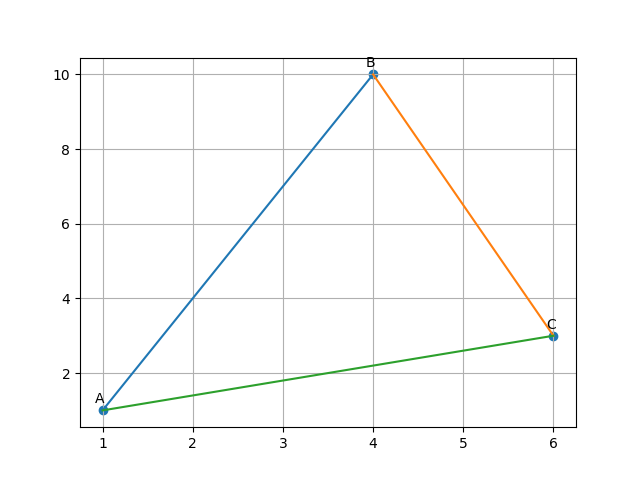
\includegraphics[width = \columnwidth]{./chapters/12/10/2/18/figs/triangle.png}
\caption{}
	\label{fig:chapters/12/10/2/18/}
\end{figure}
\solution
		\iffalse
\documentclass[journal,12pt,twocolumn]{IEEEtran}
\usepackage{romannum}
\usepackage{float}
\usepackage{setspace}
\usepackage{gensymb}
\singlespacing
\usepackage[cmex10]{amsmath}
\usepackage{amsthm}
\usepackage{mathrsfs}
\usepackage{txfonts}
\usepackage{stfloats}
\usepackage{bm}
\usepackage{cite}
\usepackage{cases}
\usepackage{subfig}
\usepackage{longtable}
\usepackage{multirow}
\usepackage{enumitem}
\usepackage{mathtools}
\usepackage{steinmetz}
\usepackage{tikz}
\usepackage{circuitikz}
\usepackage{verbatim}
\usepackage{tfrupee}
\usepackage[breaklinks=true]{hyperref}
\usepackage{tkz-euclide}
\usetikzlibrary{calc,math}
\usepackage{listings}
    \usepackage{color}                                            %%
    \usepackage{array}                                            %%
    \usepackage{longtable}                                        %%
    \usepackage{calc}                                             %%
    \usepackage{multirow}                                         %%
    \usepackage{hhline}                                           %%
    \usepackage{ifthen}                                           %%
  %optionally (for landscape tables embedded in another document): %%
    \usepackage{lscape}     
\usepackage{multicol}
\usepackage{chngcntr}
\DeclareMathOperator*{\Res}{Res}
\renewcommand\thesection{\arabic{section}}
\renewcommand\thesubsection{\thesection.\arabic{subsection}}
\renewcommand\thesubsubsection{\thesubsection.\arabic{subsubsection}}

\renewcommand\thesectiondis{\arabic{section}}
\renewcommand\thesubsectiondis{\thesectiondis.\arabic{subsection}}
\renewcommand\thesubsubsectiondis{\thesubsectiondis.\arabic{subsubsection}}

% correct bad hyphenation here
\hyphenation{op-tical net-works semi-conduc-tor}
\def\inputGnumericTable{}                                 %%

\lstset{
frame=single, 
breaklines=true,
columns=fullflexible
}

\begin{document}


\newtheorem{theorem}{Theorem}[section]
\newtheorem{problem}{Problem}
\newtheorem{proposition}{Proposition}[section]
\newtheorem{lemma}{Lemma}[section]
\newtheorem{corollary}[theorem]{Corollary}
\newtheorem{example}{Example}[section]
\newtheorem{definition}[problem]{Definition}
\newcommand{\BEQA}{\begin{eqnarray}}
\newcommand{\EEQA}{\end{eqnarray}}
\newcommand{\define}{\stackrel{\triangle}{=}}

\bibliographystyle{IEEEtran}
\providecommand{\mbf}{\mathbf}
\providecommand{\pr}[1]{\ensuremath{\Pr\left(#1\right)}}
\providecommand{\qfunc}[1]{\ensuremath{Q\left(#1\right)}}
\providecommand{\sbrak}[1]{\ensuremath{{}\left[#1\right]}}
\providecommand{\lsbrak}[1]{\ensuremath{{}\left[#1\right.}}
\providecommand{\rsbrak}[1]{\ensuremath{{}\left.#1\right]}}
\providecommand{\brak}[1]{\ensuremath{\left(#1\right)}}
\providecommand{\lbrak}[1]{\ensuremath{\left(#1\right.}}
\providecommand{\rbrak}[1]{\ensuremath{\left.#1\right)}}
\providecommand{\cbrak}[1]{\ensuremath{\left\{#1\right\}}}
\providecommand{\lcbrak}[1]{\ensuremath{\left\{#1\right.}}
\providecommand{\rcbrak}[1]{\ensuremath{\left.#1\right\}}}
\theoremstyle{remark}
\newtheorem{rem}{Remark}
\newcommand{\sgn}{\mathop{\mathrm{sgn}}}
\providecommand{\abs}[1]{\left\vert#1\right\vert}
\providecommand{\res}[1]{\Res\displaylimits_{#1}} 
\providecommand{\norm}[1]{\left\lVert#1\right\rVert}
\providecommand{\mtx}[1]{\mathbf{#1}}
\providecommand{\mean}[1]{E\left[ #1 \right]}
\providecommand{\fourier}{\overset{\mathcal{F}}{ \rightleftharpoons}}
\providecommand{\system}{\overset{\mathcal{H}}{ \longleftrightarrow}}
\newcommand{\solution}{\noindent \textbf{Solution: }}
\newcommand{\cosec}{\,\text{cosec}\,}
\providecommand{\dec}[2]{\ensuremath{\overset{#1}{\underset{#2}{\gtrless}}}}
\newcommand{\myvec}[1]{\ensuremath{\begin{pmatrix}#1\end{pmatrix}}}
\newcommand{\mydet}[1]{\ensuremath{\begin{vmatrix}#1\end{vmatrix}}}
\numberwithin{equation}{subsection}
\makeatletter
\@addtoreset{figure}{problem}
\makeatother

\let\StandardTheFigure\thefigure
\let\vec\mathbf
\renewcommand{\thefigure}{\theproblem}



\def\putbox#1#2#3{\makebox[0in][l]{\makebox[#1][l]{}\raisebox{\baselineskip}[0in][0in]{\raisebox{#2}[0in][0in]{#3}}}}
     \def\rightbox#1{\makebox[0in][r]{#1}}
     \def\centbox#1{\makebox[0in]{#1}}
     \def\topbox#1{\raisebox{-\baselineskip}[0in][0in]{#1}}
     \def\midbox#1{\raisebox{-0.5\baselineskip}[0in][0in]{#1}}

\vspace{3cm}


\title{Assignment 1}
\author{Jaswanth Chowdary Madala}





% make the title area
\maketitle

\newpage

%\tableofcontents

\bigskip

\renewcommand{\thefigure}{\theenumi}
\renewcommand{\thetable}{\theenumi}

\begin{enumerate}
\item In the following figure for the triangle ABC, which of the following is not true:

(A) $\overrightarrow{AB}+\overrightarrow{BC}+\overrightarrow{CA} = \overrightarrow{0}$

(B) $\overrightarrow{AB}+\overrightarrow{BC}-\overrightarrow{AC} = \overrightarrow{0}$

(C) $\overrightarrow{AB}+\overrightarrow{BC}+\overrightarrow{AC} = \overrightarrow{0}$

(D) $\overrightarrow{AB}-\overrightarrow{CB}+\overrightarrow{CA} = \overrightarrow{0}$

\textbf{Solution:}
\fi
		We know that,
\begin{align}
\overrightarrow{AB} = \vec{B} - \vec{A}\\
\overrightarrow{BC} = \vec{C} - \vec{B}\\
\overrightarrow{CA} = \vec{A} - \vec{C}
\end{align}
By usinig this we verify each of the given option

\begin{enumerate}
\item 
\begin{align}
\overrightarrow{AB}+\overrightarrow{BC}+\overrightarrow{CA} &=
\vec{B}-\vec{A} + \vec{C} - \vec{B} + \vec{A} - \vec{C}\\
 &= 0
\end{align}
Option A is correct.

\item
\begin{align}
\overrightarrow{AB}+\overrightarrow{BC}-\overrightarrow{AC} &=
\vec{B}-\vec{A} + \vec{C} - \vec{B} - (\vec{C} - \vec{A})\\
 &= 0
\end{align}
Option B is correct.

\item 
\begin{align}
\overrightarrow{AB}+\overrightarrow{BC}+\overrightarrow{AC} &=
\vec{B}-\vec{A} + \vec{C} - \vec{B} + \vec{C} - \vec{A}\\
 &= 2(\vec{C}-\vec{A})
\end{align}
Option C is incorrect.

\item
\begin{align}
\overrightarrow{AB}-\overrightarrow{CB}+\overrightarrow{CA} &=
\vec{B}-\vec{A} - (\vec{B} - \vec{C}) + \vec{A} - \vec{C}\\
 &= 0
\end{align}
Option D is correct.
\end{enumerate}
Verification: Let us take an example to verify 
\begin{align}
\vec{A} = \myvec{1\\1}, 
\vec{B} = \myvec{3\\1},
\vec{C} = \myvec{6\\6} \\
\overrightarrow{AB} = \vec{B} - \vec{A} = \myvec{2\\0}, 
\overrightarrow{BC} = \vec{C} - \vec{B} = \myvec{3\\5},
\overrightarrow{CA} = \vec{A} - \vec{C} = \myvec{-5\\-5} 
\end{align}
Thus,
\begin{align}
\overrightarrow{AB}+\overrightarrow{BC}+\overrightarrow{CA} = \myvec{2+3+(-5) \\ 0+5+(-5)} = \myvec{0 \\0}
\end{align}
Similarly other options can be verified.



\item If $\vec{a}$ and $\vec{b}$ are two collinear vectors, then which of the following are incorrect:
\begin{enumerate}
    \item $\vec{b}=\lambda\vec{a},$
 for some scalar $\lambda$
    \item $\vec{a}=\pm\vec{b}$
    \item the respective components of $\vec{a}$ and $\vec{b}$ are not proportiona
    \item both the vectors $\vec{a}$ and $\vec{b}$ have same direction, but different magnitudes.
\end{enumerate}
\end{enumerate}

\section{3D-Properties}
\begin{enumerate}[label=\thesection.\arabic*,ref=\thesection.\theenumi]
	\item Find the direction cosines of the sides of a triangle whose vertices are $\myvec{3\\ 5\\-4 }$, $\myvec{ -1\\1 \\2 }$ and $\myvec{-5 \\-5 \\-2 }$.
		\\
		\solution
		\iffalse
\documentclass[journal,12pt,twocolumn]{IEEEtran}
%
\usepackage{setspace}
\usepackage{gensymb}
%\doublespacing
\singlespacing

%\usepackage{graphicx}
%\usepackage{amssymb}
%\usepackage{relsize}
\usepackage[cmex10]{amsmath}
%\usepackage{amsthm}
%\interdisplaylinepenalty=2500
%\savesymbol{iint}
%\usepackage{txfonts}
%\restoresymbol{TXF}{iint}
%\usepackage{wasysym}
\usepackage{amsthm}
%\usepackage{iithtlc}
\usepackage{mathrsfs}
\usepackage{txfonts}
\usepackage{stfloats}
\usepackage{bm}
\usepackage{cite}
\usepackage{cases}
\usepackage{subfig}
%\usepackage{xtab}
\usepackage{longtable}
\usepackage{multirow}
%\usepackage{algorithm}
%\usepackage{algpseudocode}
\usepackage{enumitem}
\usepackage{mathtools}
\usepackage{steinmetz}
\usepackage{tikz}
\usepackage{circuitikz}
\usepackage{verbatim}
\usepackage{tfrupee}
\usepackage[breaklinks=true]{hyperref}
%\usepackage{stmaryrd}
\usepackage{tkz-euclide} % loads  TikZ and tkz-base
%\usetkzobj{all}
\usetikzlibrary{calc,math}
\usepackage{listings}
    \usepackage{color}                                            %%
    \usepackage{array}                                            %%
    \usepackage{longtable}                                        %%
    \usepackage{calc}                                             %%
    \usepackage{multirow}                                         %%
    \usepackage{hhline}                                           %%
    \usepackage{ifthen}                                           %%
  %optionally (for landscape tables embedded in another document): %%
    \usepackage{lscape}     
\usepackage{multicol}
\usepackage{chngcntr}
%\usepackage{enumerate}

%\usepackage{wasysym}
%\newcounter{MYtempeqncnt}
\DeclareMathOperator*{\Res}{Res}
%\renewcommand{\baselinestretch}{2}
\renewcommand\thesection{\arabic{section}}
\renewcommand\thesubsection{\thesection.\arabic{subsection}}
\renewcommand\thesubsubsection{\thesubsection.\arabic{subsubsection}}

\renewcommand\thesectiondis{\arabic{section}}
\renewcommand\thesubsectiondis{\thesectiondis.\arabic{subsection}}
\renewcommand\thesubsubsectiondis{\thesubsectiondis.\arabic{subsubsection}}

% correct bad hyphenation here
\hyphenation{op-tical net-works semi-conduc-tor}
\def\inputGnumericTable{}                                 %%

\lstset{
%language=C,
frame=single, 
breaklines=true,
columns=fullflexible
}
%\lstset{
%language=tex,
%frame=single, 
%breaklines=true
%}

\begin{document}
%


\newtheorem{theorem}{Theorem}[section]
\newtheorem{problem}{Problem}
\newtheorem{proposition}{Proposition}[section]
\newtheorem{lemma}{Lemma}[section]
\newtheorem{corollary}[theorem]{Corollary}
\newtheorem{example}{Example}[section]
\newtheorem{definition}[problem]{Definition}
%\newtheorem{thm}{Theorem}[section] 
%\newtheorem{defn}[thm]{Definition}
%\newtheorem{algorithm}{Algorithm}[section]
%\newtheorem{cor}{Corollary}
\newcommand{\BEQA}{\begin{eqnarray}}
\newcommand{\EEQA}{\end{eqnarray}}
\newcommand{\define}{\stackrel{\triangle}{=}}

\bibliographystyle{IEEEtran}
%\bibliographystyle{ieeetr}


\providecommand{\mbf}{\mathbf}
\providecommand{\pr}[1]{\ensuremath{\Pr\left(#1\right)}}
\providecommand{\qfunc}[1]{\ensuremath{Q\left(#1\right)}}
\providecommand{\sbrak}[1]{\ensuremath{{}\left[#1\right]}}
\providecommand{\lsbrak}[1]{\ensuremath{{}\left[#1\right.}}
\providecommand{\rsbrak}[1]{\ensuremath{{}\left.#1\right]}}
\providecommand{\brak}[1]{\ensuremath{\left(#1\right)}}
\providecommand{\lbrak}[1]{\ensuremath{\left(#1\right.}}
\providecommand{\rbrak}[1]{\ensuremath{\left.#1\right)}}
\providecommand{\cbrak}[1]{\ensuremath{\left\{#1\right\}}}
\providecommand{\lcbrak}[1]{\ensuremath{\left\{#1\right.}}
\providecommand{\rcbrak}[1]{\ensuremath{\left.#1\right\}}}
\theoremstyle{remark}
\newtheorem{rem}{Remark}
\newcommand{\sgn}{\mathop{\mathrm{sgn}}}
\providecommand{\abs}[1]{\left\vert#1\right\vert}
\providecommand{\res}[1]{\Res\displaylimits_{#1}} 
\providecommand{\norm}[1]{\left\lVert#1\right\rVert}
%\providecommand{\norm}[1]{\lVert#1\rVert}
\providecommand{\mtx}[1]{\mathbf{#1}}
\providecommand{\mean}[1]{E\left[ #1 \right]}
\providecommand{\fourier}{\overset{\mathcal{F}}{ \rightleftharpoons}}
%\providecommand{\hilbert}{\overset{\mathcal{H}}{ \rightleftharpoons}}
\providecommand{\system}{\overset{\mathcal{H}}{ \longleftrightarrow}}
	%\newcommand{\solution}[2]{\textbf{Solution:}{#1}}
\newcommand{\solution}{\noindent \textbf{Solution: }}
\newcommand{\cosec}{\,\text{cosec}\,}
\providecommand{\dec}[2]{\ensuremath{\overset{#1}{\underset{#2}{\gtrless}}}}
\newcommand{\myvec}[1]{\ensuremath{\begin{pmatrix}#1\end{pmatrix}}}
\newcommand{\mydet}[1]{\ensuremath{\begin{vmatrix}#1\end{vmatrix}}}
%\numberwithin{equation}{section}
\numberwithin{equation}{subsection}
%\numberwithin{problem}{section}
%\numberwithin{definition}{section}
\makeatletter
\@addtoreset{figure}{problem}
\makeatother

\let\StandardTheFigure\thefigure
\let\vec\mathbf
%\renewcommand{\thefigure}{\theproblem.\arabic{figure}}
\renewcommand{\thefigure}{\theproblem}
%\setlist[enumerate,1]{before=\renewcommand\theequation{\theenumi.\arabic{equation}}
%\counterwithin{equation}{enumi}


%\renewcommand{\theequation}{\arabic{subsection}.\arabic{equation}}

\def\putbox#1#2#3{\makebox[0in][l]{\makebox[#1][l]{}\raisebox{\baselineskip}[0in][0in]{\raisebox{#2}[0in][0in]{#3}}}}
     \def\rightbox#1{\makebox[0in][r]{#1}}
     \def\centbox#1{\makebox[0in]{#1}}
     \def\topbox#1{\raisebox{-\baselineskip}[0in][0in]{#1}}
     \def\midbox#1{\raisebox{-0.5\baselineskip}[0in][0in]{#1}}

\vspace{3cm}


\title{Question: 12.11.1.5}
\author{Nikam Pratik Balasaheb (EE21BTECH11037)}





% make the title area
\maketitle

\newpage

%\tableofcontents

\bigskip

\renewcommand{\thefigure}{\theenumi}
\renewcommand{\thetable}{\theenumi}
%\renewcommand{\theequation}{\theenumi}

\section{Problem}
\section{Solution}
\fi
Let the vertices be
\begin{align}
\vec{A} = \myvec{3\\5\\-4},
\vec{B} = \myvec{-1\\1\\2},
\vec{C} = \myvec{-5\\-5\\-2}
\end{align}
%
The direction vectors of the sides are,
\begin{align}
\vec{A} - \vec{B} = \myvec{4\\4\\-6} = \vec{m_1},
\vec{B} - \vec{C} = \myvec{4\\6\\4} = \vec{m_2}, 
\vec{C} - \vec{A} = \myvec{-8\\-10\\2} =\vec{m_3},
\end{align}
%
The direction vectors of the axes are,
\begin{align}
\vec{e}_1 = \myvec{1\\0\\0},
\vec{e}_2 = \myvec{0\\1\\0},
\vec{e}_3 = \myvec{0\\0\\1}
\end{align}
Direction cosines of a vector $\vec{m}$ are given by
\begin{align}
\myvec{\cos{\theta_1}\\ \cos{\theta_2}\\\cos{\theta_3}} = \myvec{ \frac{\vec{m}^{\top} {\vec{e}_1}}{\norm{\vec{m}}\norm{\vec{e}_1} }  \\[1pt] \frac{\vec{m}^{\top} {\vec{e}_1}}{\norm{\vec{m}}\norm{\vec{e}_1} } \\[1pt] \frac{\vec{m}^{\top} {\vec{e}_1}}{\norm{\vec{m}}\norm{\vec{e}_1} } }
= \frac{1}{\norm{\vec{m}}}\myvec{ \vec{m}^{\top} {\vec{e}_1} \\ \vec{m}^{\top} {\vec{e}_2} \\ \vec{m}^{\top} {\vec{e}_3} }
= \frac{\vec{m}}{\norm{\vec{m}}}
\end{align}
Direction cosines of side $\vec{m_1}$ are
\begin{align}
\myvec{\cos{\theta_1}\\ \cos{\theta_2}\\\cos{\theta_3}} = \frac{\vec{m_1}}{\norm{\vec{m_1}}}
= \myvec{ \frac{2}{\sqrt{17}} \\[1pt] \frac{2}{\sqrt{17}} \\[1pt] \frac{-3}{\sqrt{17}} } 
\end{align}
Direction cosines of side $\vec{m_2}$ are,
\begin{align}
\myvec{\cos{\theta_1}\\ \cos{\theta_2}\\\cos{\theta_3}} = \frac{\vec{m_2}}{\norm{\vec{m_2}}}
= \myvec{ \frac{2}{\sqrt{17}} \\[1pt] \frac{3}{\sqrt{17}} \\[1pt] \frac{2}{\sqrt{17}} } 
\end{align}
Direction cosines of side $\vec{m_3}$ are,
\begin{align}
\myvec{\cos{\theta_1}\\ \cos{\theta_2}\\\cos{\theta_3}} = \frac{\vec{m_3}}{\norm{\vec{m_3}}}
= \myvec{ \frac{-4}{\sqrt{42}} \\[1pt] \frac{-5}{\sqrt{42}} \\[1pt] \frac{1}{\sqrt{42}} } 
\end{align}
\iffalse

\begin{figure}[h!]
  \centering
   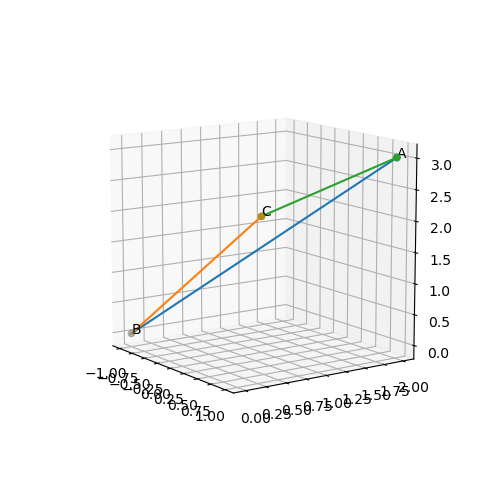
\includegraphics[width=\linewidth]{figs/Figure_1.png}
   \caption{Triangle ABC}
   \label{fig:TriangleABC}
\end{figure}

\end{document}


\fi

\end{enumerate}


\section{Scalar Product}
\iffalse
\documentclass[12pt]{article}
\usepackage{graphicx}
\usepackage{commath}
\usepackage{gensymb}

\begin{document}
\begin{center}
\textbf\large{CHAPTER-10 \\ VECTOR ALGEBRA}
\end{center}

\section{EXERCISE - 10.3}
\begin{enumerate}
		\fi
\begin{enumerate}[label=\thesection.\arabic*,ref=\thesection.\theenumi]
\item Find the angle between two vectors $\overrightarrow{a}$ and $\overrightarrow {b} $ with magnitudes $\sqrt{3}$ and 2 respectively having $\overrightarrow {a}.\overrightarrow {b}=\sqrt{6}$.
\item Find the angle between the the vectors $\hat{i}-2\hat{j}+3\hat{k}$ and $3\hat{i}-2\hat{j}+\hat{k}$.
\item Find the projection of the vector $\hat{i}-\hat{j}$ on the vector $\hat{i}+\hat{j}$.
	\\
		\iffalse
\documentclass[12pt]{chapters/10/7/4/3/figsarticle}
\usepackage{graphicx}
\usepackage[none]{chapters/10/7/4/3/figshyphenat}
\usepackage{graphicx}
\usepackage{listings}
\usepackage[english]{chapters/10/7/4/3/figsbabel}
\usepackage{graphicx}
\usepackage{caption} 
\usepackage{booktabs}
\usepackage{array}
\usepackage{amssymb} % for \because
\usepackage{amsmath}   % for having text in math mode
\usepackage{extarrows} % for Row operations arrows
\usepackage{listings}
\lstset{
  frame=single,
  breaklines=true
}
\usepackage{hyperref}
  
%Following 2 lines were added to remove the blank page at the beginning
\usepackage{atbegshi}% http://ctan.org/pkg/atbegshi
\AtBeginDocument{\AtBeginShipoutNext{\AtBeginShipoutDiscard}}


%New macro definitions
\newcommand{\mydet}[1]{chapters/10/7/4/3/figs\ensuremath{\begin{vmatrix}#1\end{vmatrix}}}
\providecommand{\brak}[1]{chapters/10/7/4/3/figs\ensuremath{\left(#1\right)}}
\newcommand{\solution}{\noindent \textbf{Solution: }}
\newcommand{\myvec}[1]{chapters/10/7/4/3/figs\ensuremath{\begin{pmatrix}#1\end{pmatrix}}}
\providecommand{\norm}[1]{chapters/10/7/4/3/figs\left\lVert#1\right\rVert}
\providecommand{\abs}[1]{chapters/10/7/4/3/figs\left\vert#1\right\vert}
\let\vec\mathbf


\begin{document}

\begin{center}
\title{\textbf{VECTORS}}
\date{\vspace{-5ex}} %Not to print date automatically
\maketitle
\end{center}

\setcounter{page}{1}

\section{10$^{th}$ Maths - Chapter 10}

This is Problem-3 from Exercise 10.3

\begin{enumerate}
\item Find the projection of the vector $\hat{i}-\hat{j}$ on the vector $\hat{i}+\hat{j}$  
\end{enumerate}
\section{SOLUTION}
\fi
\solution
The given points are
\begin{align}
 \vec{A}=\myvec{1\\ -1},
 \vec{B}=\myvec{1\\ 1}
\end{align}
Since
\begin{align}
	\vec{A}^\top \vec{B} &= \myvec{1 &-1} \myvec{1\\ 1}=\myvec{1 \times 1}+\myvec{-1 \times  1}=0
	\\
	\norm {\vec {B}}^2 &= (\vec{B}^\top  \vec{B})=\myvec{1 & 1} \myvec{1\\ 1}= (1 \times  1)+(1 \times  1)=2,
\end{align}
and the project vector is given by 
\begin{align}
	\vec{C} &= 
	\frac{\vec{A}^\top  \vec{B}}{\norm {\vec{B}}}^2 \vec{B}
	&=\frac{0}{2} \myvec{1\\ 1}
	=\myvec{0\\ 0}
\end{align}
This is verfied in Fig.
		\ref{fig:12/10/3/3Figure}.
\begin{figure}[h]
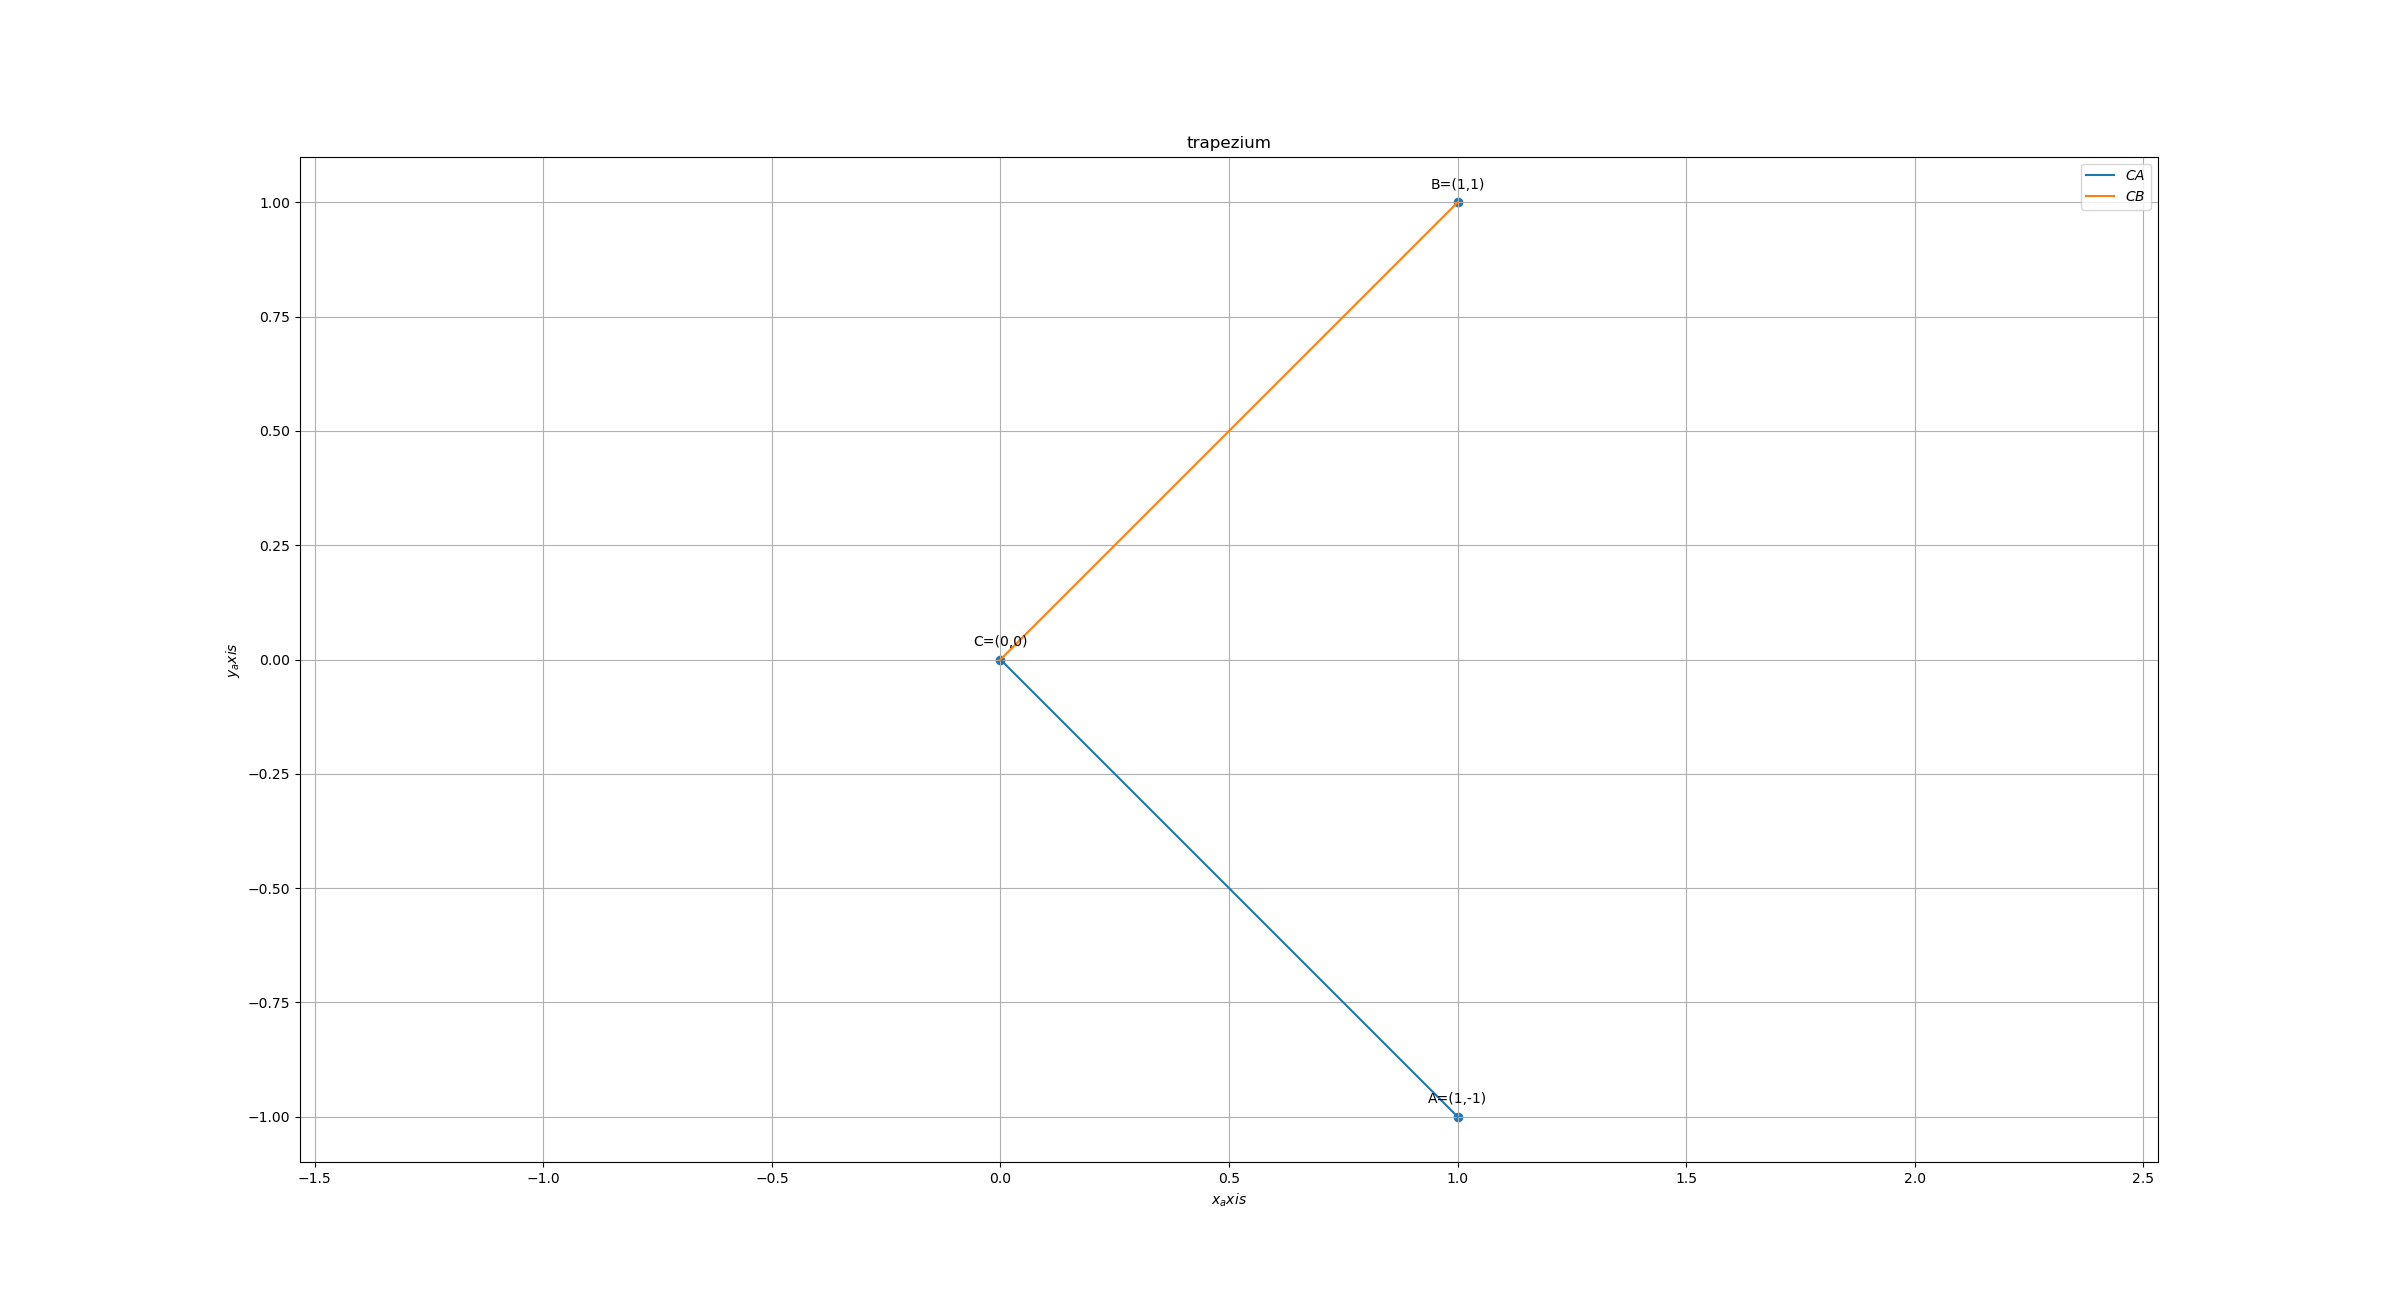
\includegraphics[width=\columnwidth]{chapters/12/10/3/3/figs/vector.png}
\caption{}
		\label{fig:12/10/3/3Figure}
\end{figure}

\item Find the projection of the vector $\hat{i}+3\hat{j}+7\hat{k}$ on the vector $7\hat{i}-\hat{j}+8\hat{k}$.
\item Show that each of the given three vectors is a unit vector: 

 $\frac{1}{7}(2\hat{i}+3\hat{j}+6\hat{k}),\frac{1}{7}(3\hat{i}-6\hat{j}+2\hat{k}),\frac{1}{7}(6\hat{i}+2\hat{j}-3\hat{k}$)
 
Also,show that they are mutually perpendicular to each other.
\item Find $\abs{\overrightarrow {a}}$ and $\abs{\overrightarrow {b}}$,if ($\overrightarrow {a}+\overrightarrow {b}).(\overrightarrow {a}-\overrightarrow {b})=8$ and $\abs{\overrightarrow {a}}=8\abs{\overrightarrow {b}}$.
\item Evaluate the product(3$\overrightarrow {a}-5\overrightarrow {b}).(2\overrightarrow {a}+7\overrightarrow {b}$).
\item Find the magnitude of two vectors $\overrightarrow {a}$ and $\overrightarrow {b}$, having the same magnitude and such that the angle between them is $60\degree$ and their scalar product is $\frac{1}{2}$
\item Find $\abs{\overrightarrow {x}}$,if for a unit vector $\overrightarrow {a},(\overrightarrow {x}-\overrightarrow {a}).(\overrightarrow {x}+\overrightarrow {a}$)=12.
	\\
		\iffalse
\documentclass[12pt]{article}
\usepackage{graphicx}
%\documentclass[journal,12pt,twocolumn]{IEEEtran}
\usepackage[none]{hyphenat}
\usepackage{graphicx}
\usepackage{listings}
\usepackage[english]{babel}
\usepackage{graphicx}
\usepackage{caption} 
\usepackage{hyperref}
\usepackage{booktabs}
\usepackage{array}
\usepackage{amsmath}   % for having text in math mode
\usepackage{listings}
\lstset{
  frame=single,
  breaklines=true
}
  
%Following 2 lines were added to remove the blank page at the beginning
\usepackage{atbegshi}% http://ctan.org/pkg/atbegshi
\AtBeginDocument{\AtBeginShipoutNext{\AtBeginShipoutDiscard}}
%


%New macro definitions
\newcommand{\mydet}[1]{\ensuremath{\begin{vmatrix}#1\end{vmatrix}}}
\providecommand{\brak}[1]{\ensuremath{\left(#1\right)}}
\providecommand{\norm}[1]{\left\lVert#1\right\rVert}
\newcommand{\solution}{\noindent \textbf{Solution: }}
\newcommand{\myvec}[1]{\ensuremath{\begin{pmatrix}#1\end{pmatrix}}}
\let\vec\mathbf

\begin{document}

\begin{center}
\title{\textbf{Vector Dot Product}}
\date{\vspace{-5ex}} %Not to print date automatically
\maketitle
\end{center}
\setcounter{page}{1}

\section{12$^{th}$ Maths - Chapter 10}
This is Problem-9 from Exercise 10.3
\begin{enumerate}
\item Find $\norm{\vec{x}}$, if for a unit vector $\vec{a}$, $\brak{\vec{x}-\vec{a}}.\brak{\vec{x}+\vec{a}} = 12$.\\
	\fi
\solution 
From the given information,
\begin{align}
  \label{eq:12/10/3/9det2f}
  \brak{\vec{x}-\vec{a}}^\top\brak{\vec{x}+\vec{a}} &= 12 \\
  \implies \vec{x}^\top\vec{x} - \vec{a}^\top\vec{x} + \vec{x}^\top\vec{a} - \vec{a}^\top\vec{a} &= 12 \\
  \implies \norm{\vec{x}}^{2} - \norm{\vec{a}}^{2} &= 12 \\
\implies   \norm{\vec{x}}^{2} - 1 &= 12  \\
	\text{or, }  
	\norm{\vec{x}} &= \sqrt{13}
\end{align}

\item If $\overrightarrow {a}=2\hat{i}+2\hat{j}3\hat{k},\overrightarrow {b}=\hat{-i}+2\hat{j}+\hat{k}$ and $\overrightarrow {c}=3\hat{i}+\hat{j}$ are such that $\overrightarrow {a}+\lambda\overrightarrow {b}$ is perpendicular to $\overrightarrow {c}$,then find the value of $\lambda$.
	\\
		\iffalse
\documentclass[12pt]{article}
\usepackage{graphicx}
\usepackage{amsmath}
\usepackage{mathtools}
\usepackage{gensymb}

\newcommand{\mydet}[1]{\ensuremath{\begin{vmatrix}#1\end{vmatrix}}}
\providecommand{\brak}[1]{\ensuremath{\left(#1\right)}}
\providecommand{\norm}[1]{\left\lVert#1\right\rVert}
\newcommand{\solution}{\noindent \textbf{Solution: }}
\newcommand{\myvec}[1]{\ensuremath{\begin{pmatrix}#1\end{pmatrix}}}
\let\vec\mathbf

\begin{document}
\begin{center}
\textbf\large{CHAPTER-10 \\ VECTOR ALGEBRA}

\end{center}
\section*{Excercise 10.3}

Q10.If $\vec{a} = 2\hat{i}+2\hat{j}+3\hat{k}, \vec{b} = -\hat{i}+2\hat{j}+\hat{k} \text{ and } \vec{c} = 3\hat{i}+\hat{j}$ are such that $\vec{a}+\lambda \vec{b}$ is perpendicular to $\vec{c}$, then find the value of $\lambda$.
\fi
\solution
Given that
\begin{align}
	(\vec{a}+\lambda \vec{b})^{\top} \vec{c} &= 0\\
\implies \vec{a}^{\top}\vec{c}+\lambda \vec{b}^{\top}\vec{c}&=0\\
\implies 	\lambda \vec{b}^{\top}\vec{c}&=-\vec{a}^{\top}\vec{c}\\
\implies 	\lambda(\vec{b}^{\top}\vec{c})(\vec{b}^{\top}\vec{c})^{-1}&=-(\vec{a}^{\top}\vec{c})(\vec{b}^{\top}\vec{c})^{-1}\\
\implies 	\lambda&=-(\vec{a}^{\top}\vec{c})(\vec{b}^{\top}\vec{c})^{-1}
\end{align}
Now substituting the values
\begin{align}
	\vec{a}^{\top}\vec{c}&=\myvec{2&2&3} \myvec{3\\1\\0} = 8\\
	\vec{b}^{\top}\vec{c}&=\myvec{-1&2&1} \myvec{3\\1\\0} = -1,
\end{align}
\begin{align}
	\lambda&=-(\vec{a}^{\top}\vec{c})(\vec{b}^{\top}\vec{c})^{-1}\\
	&=-(8)(-1)^{-1}\\
	&=8
\end{align}



\item Show that $\abs {\overrightarrow {a}}\overrightarrow {b}+\abs{\overrightarrow {b}}\overrightarrow {a}$ is perpendicular to $\abs{\overrightarrow {a}} \overrightarrow {b}-\abs{\overrightarrow {b}} \overrightarrow {a}$, for any two nonzero vectors $\overrightarrow {a}$ and $\overrightarrow {b}$.
\item If $\overrightarrow {a}.\overrightarrow {a}$=0 and $\overrightarrow {a}.\overrightarrow {b}$=0, then what can be conculded about the vector $\overrightarrow {b}$?
\item If $\overrightarrow {a},\overrightarrow {b},\overrightarrow {c}$ are unit vectors such that $\overrightarrow {a}+\overrightarrow {b}+\overrightarrow {c}=\overrightarrow {0}$, find the value of $\overrightarrow {a}.\overrightarrow {b}+\overrightarrow {b}.\overrightarrow {c}+\overrightarrow {c}.\overrightarrow {a}$.
\item If either vector $\overrightarrow {a}=0$ or $\overrightarrow {b}=0$, then $\overrightarrow {a}.\overrightarrow {b}$=0. But the converse need not be true .Justify your answer with an example.
\item If the vertices A,B,C of a triangle ABC are (1,2,3),(-1,0,0)(0,1,2), respectively , then find  $\angle{ABC}. [\angle{ABC}$ is the angle between the vectors $\overrightarrow{BA}$ and $\overrightarrow{BC}$].
\item show that the points A(1,2,7),B(2,6,3)and C(3,10,-1) are collinear.
\item show that the vectors $2\hat{i}-\hat{j}+\hat{k},\hat{i}-3\hat{j}-5\hat{k}$ and  $3\hat{i}-4\hat{j}-4\hat{k}$ from the vertices of a right angled triangle.
\item If $\overrightarrow {a}$ is a nonzero vector of magnitude 'a' and $\lambda$ a nonzero scalar , then $\lambda\overrightarrow {a}$ is unit vector if

\begin{enumerate} 
\item $\lambda=1$ 
\item $\lambda=-1$
\item $a=\abs{\lambda}$
\item $a=1/\abs{\lambda}$  
\end{enumerate}
\iffalse
\item If $\overrightarrow {a}=2\hat{i}+2\hat{j}3\hat{k},\overrightarrow {b}=\hat{-i}+2\hat{j}+\hat{k}$ and $\overrightarrow {c}=3\hat{i}+\hat{j}$ are such that $\overrightarrow {a}+\lambda\overrightarrow {b}$ is perpendicular to $\overrightarrow {c}$,then find the value of $\lambda$.
	\\
		\iffalse
\documentclass[12pt]{article}
\usepackage{graphicx}
\usepackage{amsmath}
\usepackage{mathtools}
\usepackage{gensymb}

\newcommand{\mydet}[1]{\ensuremath{\begin{vmatrix}#1\end{vmatrix}}}
\providecommand{\brak}[1]{\ensuremath{\left(#1\right)}}
\providecommand{\norm}[1]{\left\lVert#1\right\rVert}
\newcommand{\solution}{\noindent \textbf{Solution: }}
\newcommand{\myvec}[1]{\ensuremath{\begin{pmatrix}#1\end{pmatrix}}}
\let\vec\mathbf

\begin{document}
\begin{center}
\textbf\large{CHAPTER-10 \\ VECTOR ALGEBRA}

\end{center}
\section*{Excercise 10.3}

Q10.If $\vec{a} = 2\hat{i}+2\hat{j}+3\hat{k}, \vec{b} = -\hat{i}+2\hat{j}+\hat{k} \text{ and } \vec{c} = 3\hat{i}+\hat{j}$ are such that $\vec{a}+\lambda \vec{b}$ is perpendicular to $\vec{c}$, then find the value of $\lambda$.
\fi
\solution
Given that
\begin{align}
	(\vec{a}+\lambda \vec{b})^{\top} \vec{c} &= 0\\
\implies \vec{a}^{\top}\vec{c}+\lambda \vec{b}^{\top}\vec{c}&=0\\
\implies 	\lambda \vec{b}^{\top}\vec{c}&=-\vec{a}^{\top}\vec{c}\\
\implies 	\lambda(\vec{b}^{\top}\vec{c})(\vec{b}^{\top}\vec{c})^{-1}&=-(\vec{a}^{\top}\vec{c})(\vec{b}^{\top}\vec{c})^{-1}\\
\implies 	\lambda&=-(\vec{a}^{\top}\vec{c})(\vec{b}^{\top}\vec{c})^{-1}
\end{align}
Now substituting the values
\begin{align}
	\vec{a}^{\top}\vec{c}&=\myvec{2&2&3} \myvec{3\\1\\0} = 8\\
	\vec{b}^{\top}\vec{c}&=\myvec{-1&2&1} \myvec{3\\1\\0} = -1,
\end{align}
\begin{align}
	\lambda&=-(\vec{a}^{\top}\vec{c})(\vec{b}^{\top}\vec{c})^{-1}\\
	&=-(8)(-1)^{-1}\\
	&=8
\end{align}



\item Show that $\abs {\overrightarrow {a}}\overrightarrow {b}+\abs{\overrightarrow {b}}\overrightarrow {a}$ is perpendicular to $\abs{\overrightarrow {a}} \overrightarrow {b}-\abs{\overrightarrow {b}} \overrightarrow {a}$, for any two nonzero vectors $\overrightarrow {a}$ and $\overrightarrow {b}$.
\item If $\overrightarrow {a}.\overrightarrow {a}$=0 and $\overrightarrow {a}.\overrightarrow {b}$=0, then what can be conculded about the vector $\overrightarrow {b}$?
\item If $\overrightarrow {a},\overrightarrow {b},\overrightarrow {c}$ are unit vectors such that $\overrightarrow {a}+\overrightarrow {b}+\overrightarrow {c}=\overrightarrow {0}$, find the value of $\overrightarrow {a}.\overrightarrow {b}+\overrightarrow {b}.\overrightarrow {c}+\overrightarrow {c}.\overrightarrow {a}$.
\item If either vector $\overrightarrow {a}=0$ or $\overrightarrow {b}=0$, then $\overrightarrow {a}.\overrightarrow {b}$=0. But the converse need not be true .Justify your answer with an example.
\item If the vertices A,B,C of a triangle ABC are (1,2,3),(-1,0,0)(0,1,2), respectively , then find  $\angle{ABC}. [\angle{ABC}$ is the angle between the vectors $\overrightarrow{BA}$ and $\overrightarrow{BC}$].
\item show that the points A(1,2,7),B(2,6,3)and C(3,10,-1) are collinear.
\item show that the vectors $2\hat{i}-\hat{j}+\hat{k},\hat{i}-3\hat{j}-5\hat{k}$ and  $3\hat{i}-4\hat{j}-4\hat{k}$ from the vertices of a right angled triangle.
\item If $\overrightarrow {a}$ is a nonzero vector of magnitude 'a' and $\lambda$ a nonzero scalar , then $\lambda\overrightarrow {a}$ is unit vector if

\begin{enumerate} 
\item $\lambda=1$ 
\item $\lambda=-1$
\item $a=\abs{\lambda}$
\item $a=1/\abs{\lambda}$  
\end{enumerate}
\fi

\end{enumerate}


\section{Area of a Triangle }
\iffalse
\documentclass[12pt]{article}
\usepackage{graphicx}
\usepackage{amsmath}   % for having text in math mode

%Following 2 lines were added to remove the blank page at the beginning
\usepackage{atbegshi}% http://ctan.org/pkg/atbegshi
\AtBeginDocument{\AtBeginShipoutNext{\AtBeginShipoutDiscard}}
%

\begin{document}

\begin{center}
\title{\textbf{Area of a Traingle}}
\date{\vspace{-5ex}} %Not to print date automatically
\maketitle
\end{center}

\setcounter{page}{1}



\section{10$^{th}$ Maths - Chapter 7}

All problems are from Exercise 7.3

\fi
%\begin{enumerate}[label=\thechapter.\arabic*,ref=\thechapter.\theenumi]
\begin{enumerate}[label=\thesection.\arabic*,ref=\thesection.\theenumi]
\numberwithin{equation}{enumi}
\numberwithin{figure}{enumi}
\numberwithin{table}{enumi}
\item Find the area of the triangle whose vertices are 
\begin{enumerate}
\item $(2, 3), (–1, 0), (2, – 4)$
\item $(–5, –1), (3, –5), (5, 2)$ 
\end{enumerate}
		\label{10/7/3/1}
\solution
		\iffalse
\documentclass[12pt]{article}
\usepackage{graphicx}
%\documentclass[journal,12pt,twocolumn]{IEEEtran}
\usepackage[none]{hyphenat}
\usepackage{graphicx}
\usepackage{listings}
\usepackage[english]{babel}
\usepackage{graphicx}
\usepackage{caption} 
\usepackage{hyperref}
\usepackage{booktabs}
\usepackage{array}
\usepackage{amsmath}   % for having text in math mode

%Following 2 lines were added to remove the blank page at the beginning
\usepackage{atbegshi}% http://ctan.org/pkg/atbegshi
\AtBeginDocument{\AtBeginShipoutNext{\AtBeginShipoutDiscard}}
%


%New macro definitions
\newcommand{\mydet}[1]{\ensuremath{\begin{vmatrix}#1\end{vmatrix}}}
\providecommand{\brak}[1]{\ensuremath{\left(#1\right)}}
\providecommand{\norm}[1]{\left\lVert#1\right\rVert}
\newcommand{\solution}{\noindent \textbf{Solution: }}
\newcommand{\myvec}[1]{\ensuremath{\begin{pmatrix}#1\end{pmatrix}}}
\let\vec\mathbf

\begin{document}

\begin{center}
\title{\textbf{Area of a Traingle}}
\date{\vspace{-5ex}} %Not to print date automatically
\maketitle
\end{center}

\setcounter{page}{1}



\section{10$^{th}$ Maths - Chapter 7}

This is Problem-1 from Exercise 7.3

\begin{enumerate}
\item Find the area of the triangle whose vertices are :
	\fi
\begin{enumerate}
\item 
In this case, the area  is given by  
  \label{prop:10/7/3/1area2d}
  \begin{align}
    \label{eq:10/7/3/1area2d}
	\frac{1}{2}\norm{\brak{\vec{A}-\vec{B}} \times \brak{\vec{A}-\vec{C}}} \\
  \end{align}
  Since
  \begin{align}
	 \vec{A}-\vec{B} =  \myvec{
  2 \\
  3 \\
 } - \myvec{
  -1 \\
  0 \\
 } = \myvec{
 3 \\
 3 \\
 }
 \\
 \vec{A}-\vec{C} =  \myvec{
  2 \\
  3 \\
 } - \myvec{
  2 \\
  -4 \\
 } = \myvec{
 0 \\
 7 \\
 }
 \end{align}
 the desired area is given by 
 \iffalse
The value of the cross product of two vectors is given by
\begin{align}
  \label{eq:10/7/3/1det2d}
  \mydet{\vec{M}} &= \mydet{\vec{A} & \vec{B}} 
  \\
  &= \mydet{a_1 & b_1\\a_2 & b_2} = a_1b_2 - a_2 b_1
\end{align}

		Therefore, \eqref{eq:10/7/3/1area2d} equals \\
		\fi
\begin{align}
	\frac{1}{2}\mydet{3 & 0\\3 & 7}  
	&=	\frac{21}{2}
\end{align}
\iffalse
\begin{figure}[!h]
	\begin{center}
		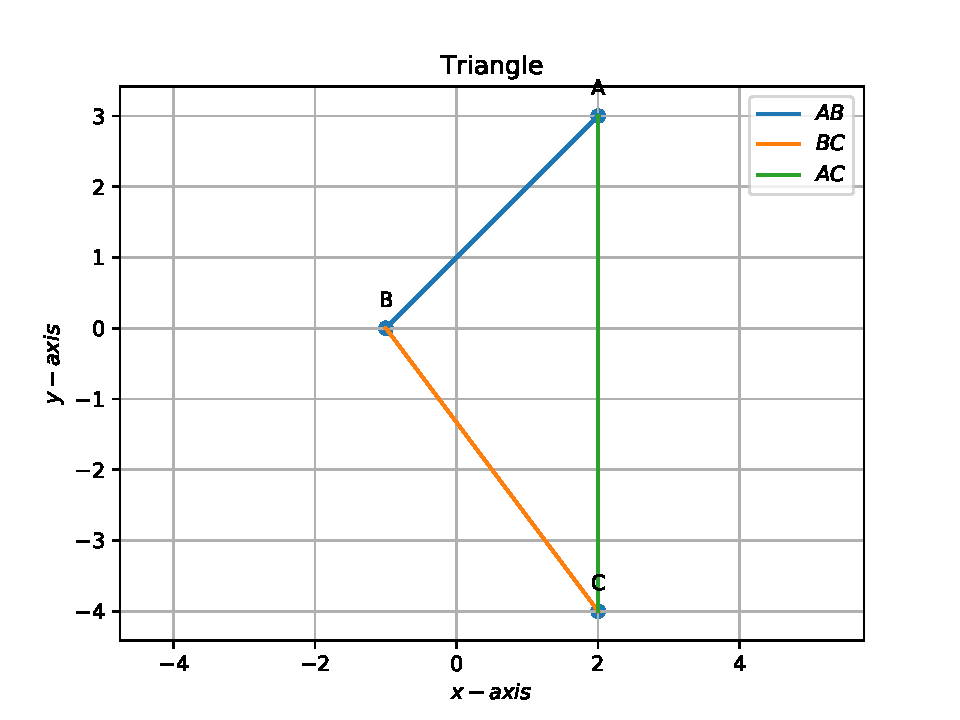
\includegraphics[width=\columnwidth]{./figs/problem1a.pdf}
	\end{center}
\caption{}
\label{fig:Fig1}
\end{figure}
\fi

\item In this case, 
	\iffalse
\solution The area of the triangle with vertices $\vec{A}, \vec{B}, \vec{C}$ is given by  
  \label{prop:10/7/3/1area2e}
  \begin{align}
    \label{eq:10/7/3/1area2e}
	\frac{1}{2}\norm{\brak{\vec{A}-\vec{B}} \times \brak{\vec{A}-\vec{C}}} \\
	\fi
  \begin{align}
	 \vec{A}-\vec{B} =  \myvec{
  -5 \\
  -1 \\
 } - \myvec{
  3 \\
  -5 \\
 } = \myvec{
 -8 \\
 4 \\
 }
 \\
 \vec{A}-\vec{C} =  \myvec{
  -5 \\
  -1 \\
 } - \myvec{
  5 \\
  2 \\
 } = \myvec{
 -10 \\
 -3 \\
 }
 \\
	  \implies
\text{Area} =	\frac{1}{2}\mydet{-8 & -10\\4 & -3}  
	=  32 
\end{align}
\iffalse
\begin{figure}[!h]
	\begin{center}
		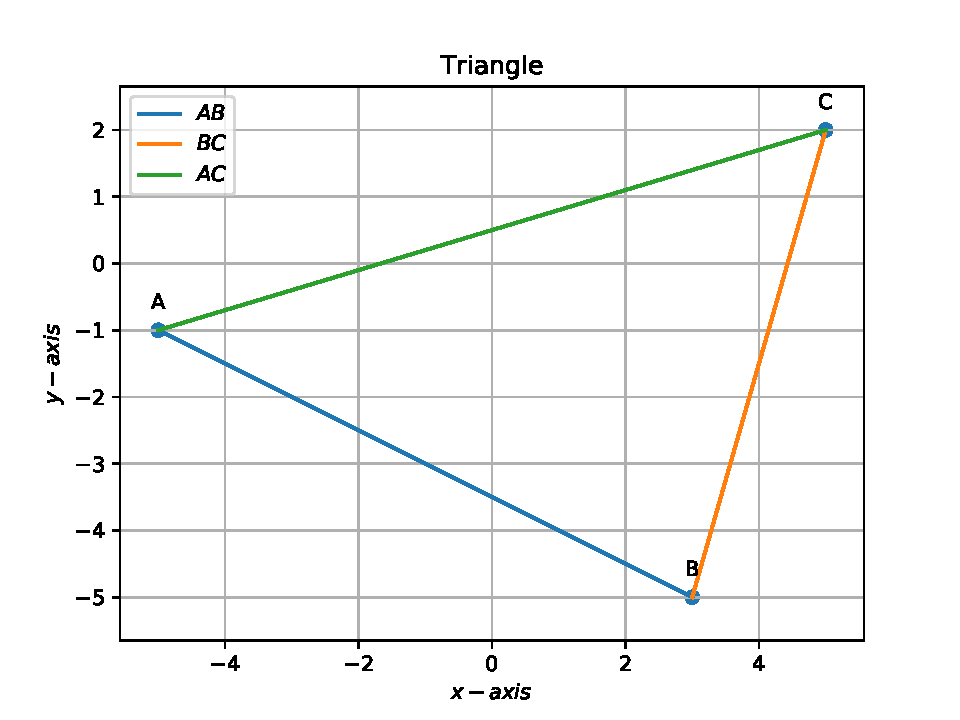
\includegraphics[width=\columnwidth]{./figs/problem1b.pdf}
	\end{center}
\caption{}
\label{fig:Fig2}
\end{figure}
\fi
\end{enumerate}




\item In each of the following, find the value of '$k$', for which the points are collinear.
\begin{enumerate}
\item $(7, –2), (5, 1), (3, k)$
\item $(8, 1), (k, – 4), (2, –5)$
\end{enumerate}
		\label{10/7/3/2}
\solution
		\iffalse
\documentclass[journal,12pt,twocolumn]{IEEEtran}
\usepackage{graphicx}
\graphicspath{{./figs/}}{}
\usepackage{amsmath,amssymb,amsfonts,amsthm}
\newcommand{\myvec}[1]{\ensuremath{\begin{pmatrix}#1\end{pmatrix}}}
\providecommand{\norm}[1]{\lVert#1\rVert}
\usepackage{listings}
\usepackage{watermark}
\usepackage{titlesec}
\usepackage{caption}
\usepackage{enumitem}
\usepackage{extarrows}
\let\vec\mathbf
\lstset{
frame=single, 
breaklines=true,
columns=fullflexible
}
\thiswatermark{\centering \put(0,-105.0){
\includegraphics[scale=0.15]{/sdcard/IITH/vector/vector-3/figs/logo.png}} }
\title{\mytitle}
\title{
Assignment - Vector-3
}
\author{Surajit Sarkar}
\begin{document}
\maketitle
\tableofcontents
\bigskip
\section{\textbf{Problem}}
In each of the following, find the value of ’k’,\\ for which the points are collinear.
\begin{enumerate}[label=(\roman*)]
\item (7, –2), (5, 1), (3, k)
\item(8, 1), (k, –4), (2, –5)
\end{enumerate}
\section{\textbf{Solution}}
\fi
\begin{enumerate}
    \item Given
    \begin{align}
      \vec{A}=\myvec{7\\-2},\Vec{B}=\myvec{5\\1},\vec{C}=\myvec{3\\k}  
    \end{align}
    Then
    \begin{align}
        \myvec{\vec{A}-\vec{B}}&=\myvec{2\\-3}\\
        \myvec{\vec{A}-\vec{C}}&=\myvec{4\\2k}\
    \end{align}
    Forming the collinearity matrix
    \begin{align}
        \myvec{2&-3\\4&2k} \xleftrightarrow{R_1\rightarrow{R_1-1}}&\myvec{1&-2\\4&2k}\\
         \xleftrightarrow{R_1\rightarrow{R_1-1}}&\myvec{1&-2\\0&2k+8}\\
        k&=4
        \end{align}
    
    \item Given
     \begin{align}
      \vec{A}=\myvec{8\\1},\vec{B}=\myvec{k\\-4},\vec{C}=\myvec{2\\-5}  
    \end{align}
    Then
    \begin{align}
        \myvec{\vec{A}-\vec{B}}&=\myvec{-8k\\-5}\\
        \myvec{\vec{A}-\vec{C}}&=\myvec{6\\6}\
    \end{align}
    Forming the collinearity matrix
    \begin{align}
        \myvec{-8-k&-5\\6&6} \xleftrightarrow{R_1\rightarrow{R_1+8}}&\myvec{-k&3\\6&6}\\
        k&=3
        \end{align}
\end{enumerate}



\item Find the area of the triangle formed by joining the mid-points of the sides of the triangle whose vertices are $(0, –1), (2, 1) \text{ and } (0, 3)$. Find the ratio of this area to the area of the given triangle.
	\\
\solution
		\iffalse
\documentclass[12pt]{article}
\usepackage{graphicx}
\usepackage{amsmath}
\usepackage{mathtools}
\usepackage{gensymb}

\newcommand{\mydet}[1]{\ensuremath{\begin{vmatrix}#1\end{vmatrix}}}
\providecommand{\brak}[1]{\ensuremath{\left(#1\right)}}
\providecommand{\norm}[1]{\left\lVert#1\right\rVert}
\newcommand{\solution}{\noindent \textbf{Solution: }}
\newcommand{\myvec}[1]{\ensuremath{\begin{pmatrix}#1\end{pmatrix}}}
\let\vec\mathbf

\begin{document}
\begin{center}
\textbf\large{CHAPTER-7 \\ COORDINATE GEOMETRY}
\end{center}
\section*{Excercise 7.2}

Q3. Find the area of the triangle formed by joining the mid-points of the sides of the triangle
whose vertices are $\vec(0, –1), \vec(2, 1) \text{ and } \vec(0, 3)$. Find the ratio of this area to the area of the
given triangle
\\
\solution
\\
\fi
The coordinates are given as
	\begin{align}
	\vec{A} = \myvec{
		0\\
		-1\\
		},
	\vec{B} = \myvec{
		2\\
		1\\
		},
	\vec{C} = \myvec{
		0\\
		3\\
		}
	\end{align}
Calculating midpoints,
	\begin{align}
		\vec{P} = \frac{1}{2}\vec(\vec{A}+\vec{B}) = \frac{1}{2}\myvec{2\\0\\} = \myvec{1\\0\\}\\
		\vec{Q} = \frac{1}{2}\vec(\vec{B}+\vec{C}) = \frac{1}{2}\myvec{2\\4\\} = \myvec{1\\2\\}\\
		\vec{R} = \frac{1}{2}\vec(\vec{A}+\vec{C}) = \frac{1}{2}\myvec{0\\2\\} = \myvec{0\\1\\}
	\end{align}
	Since
	\begin{align}
		\vec{P}-\vec{Q} &=  \myvec{
  1 \\
  0 
 } - \myvec{
  1 \\
  2 
 } = \myvec{
 0 \\
 -2 
 }
		\\
		\vec{Q}-\vec{R} &=  \myvec{
  1 \\
  2 \\
 } - \myvec{
  0 \\
  1 \\
 } = \myvec{
 1 \\
 1 \\
 }
	\end{align}
	the area is obtained as
	\begin{align}
		ar(PQR)&=\frac{1}{2}{\norm{\vec(\vec{P}-\vec{Q})\times\vec(\vec{Q}-\vec{R})}}
		\\
		&=\frac{1}{2}\mydet{0 & 1\\-2 & 1}
		=1
	\end{align}
	Similarly, 
	\begin{align}
		\vec{A}-\vec{B} &=  \myvec{
  0 \\
  -1 \\
 } - \myvec{
  2 \\
  1 \\
 } = \myvec{
 -2 \\
 -2 \\
 }
 \\
		\vec{A}-\vec{C} &=  \myvec{
  0 \\
  -1 \\
 } - \myvec{
  0 \\
  3 \\
 } = \myvec{
 0 \\
 -4 \\
 }
	\end{align}
 the area is obained as
	\begin{align}
		ar(ABC)&=\frac{1}{2}{\norm{\vec(\vec{A}-\vec{B})\times\vec(\vec{A}-\vec{C})}}\\
		&=\frac{1}{2}\mydet{-2 & 0\\-2 & -4}
=4
	\end{align}
	Thus, the resultant ratio of two areas is 1:4.
	See Fig.
\ref{fig:10/7/3/3Fig}
\begin{figure}[!h]
	\begin{center} 
	    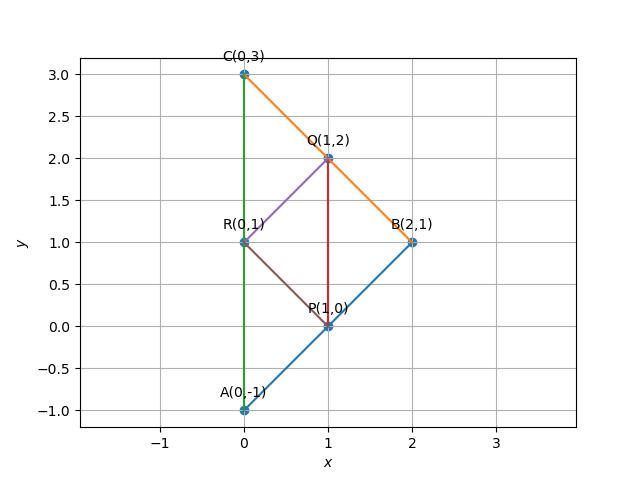
\includegraphics[width=\columnwidth]{chapters/10/7/3/3/figs/trigraph.png}
	\end{center}
\caption{}
\label{fig:10/7/3/3Fig}
\end{figure}


\item Find the area of the quadrilateral whose vertices, taken in order, are $(– 4, – 2), (– 3, – 5), (3, – 2)$  and $ (2, 3)$.
	\\
\solution
		\iffalse
\documentclass[12pt]{article}
\usepackage{graphicx}
%\documentclass[journal,12pt,twocolumn]{IEEEtran}
\usepackage[none]{hyphenat}
\usepackage{graphicx}
\usepackage{listings}
\usepackage[english]{babel}
\usepackage{graphicx}
\usepackage{caption} 
\usepackage{hyperref}
\usepackage{booktabs}
\def\inputGnumericTable{}
\usepackage{color}                                            %%
    \usepackage{array}                                            %%
    \usepackage{longtable}                                        %%
    \usepackage{calc}                                             %%
    \usepackage{multirow}                                         %%
    \usepackage{hhline}                                           %%
    \usepackage{ifthen}
\usepackage{array}
\usepackage{amsmath}   % for having text in math mode
\usepackage{listings}
\lstset{
language=tex,
frame=single, 
breaklines=true
}
  
%Following 2 lines were added to remove the blank page at the beginning
\usepackage{atbegshi}% http://ctan.org/pkg/atbegshi
\AtBeginDocument{\AtBeginShipoutNext{\AtBeginShipoutDiscard}}
%
%New macro definitions
\newcommand{\mydet}[1]{\ensuremath{\begin{vmatrix}#1\end{vmatrix}}}
\providecommand{\brak}[1]{\ensuremath{\left(#1\right)}}
\providecommand{\norm}[1]{\left\lVert#1\right\rVert}
\newcommand{\solution}{\noindent \textbf{Solution: }}
\newcommand{\myvec}[1]{\ensuremath{\begin{pmatrix}#1\end{pmatrix}}}
\let\vec\mathbf
\begin{document}
\begin{center}
\title{\textbf{Coordinate Geometry}}
\date{\vspace{-5ex}} %Not to print date automatically
\maketitle
\end{center}
\setcounter{page}{1}
\section*{10$^{th}$ Maths - Chapter 7}
This is Problem-4 from Exercise 7.3
\begin{enumerate}
\item Find the area of quadrilateral whose vertices, taken in order, are $\myvec{-4 \\ -2}, \myvec{-3\\-5}, \myvec{3\\-2}$ and $\myvec{2\\3}$.\\
	\solution 
\fi
		The input parameters for this problem are available in Table \eqref{tab:10/7/3/4}.
\begin{table}[ht!]\centering
%%%%%%%%%%%%%%%%%%%%%%%%%%%%%%%%%%%%%%%%%%%%%%%%%%%%%%%%%%%%%%%%%%%%%%
%%                                                                  %%
%%  This is the header of a LaTeX2e file exported from Gnumeric.    %%
%%                                                                  %%
%%  This file can be compiled as it stands or included in another   %%
%%  LaTeX document. The table is based on the longtable package so  %%
%%  the longtable options (headers, footers...) can be set in the   %%
%%  preamble section below (see PRAMBLE).                           %%
%%                                                                  %%
%%  To include the file in another, the following two lines must be %%
%%  in the including file:                                          %%
%%        \def\inputGnumericTable{}                                 %%
%%  at the beginning of the file and:                               %%
%%        \input{name-of-this-file.tex}                             %%
%%  where the table is to be placed. Note also that the including   %%
%%  file must use the following packages for the table to be        %%
%%  rendered correctly:                                             %%
%%    \usepackage[latin1]{inputenc}                                 %%
%%    \usepackage{color}                                            %%
%%    \usepackage{array}                                            %%
%%    \usepackage{longtable}                                        %%
%%    \usepackage{calc}                                             %%
%%    \usepackage{multirow}                                         %%
%%    \usepackage{hhline}                                           %%
%%    \usepackage{ifthen}                                           %%
%%  optionally (for landscape tables embedded in another document): %%
%%    \usepackage{lscape}                                           %%
%%                                                                  %%
%%%%%%%%%%%%%%%%%%%%%%%%%%%%%%%%%%%%%%%%%%%%%%%%%%%%%%%%%%%%%%%%%%%%%%



%%  This section checks if we are begin input into another file or  %%
%%  the file will be compiled alone. First use a macro taken from   %%
%%  the TeXbook ex 7.7 (suggestion of Han-Wen Nienhuys).            %%
\def\ifundefined#1{\expandafter\ifx\csname#1\endcsname\relax}


%%  Check for the \def token for inputed files. If it is not        %%
%%  defined, the file will be processed as a standalone and the     %%
%%  preamble will be used.                                          %%
\ifundefined{inputGnumericTable}

%%  We must be able to close or not the document at the end.        %%
 \def\gnumericTableEnd{\end{document}}


%%%%%%%%%%%%%%%%%%%%%%%%%%%%%%%%%%%%%%%%%%%%%%%%%%%%%%%%%%%%%%%%%%%%%%
%%                                                                  %%
%%  This is the PREAMBLE. Change these values to get the right      %%
%%  paper size and other niceties.                                  %%
%%                                                                  %%
%%%%%%%%%%%%%%%%%%%%%%%%%%%%%%%%%%%%%%%%%%%%%%%%%%%%%%%%%%%%%%%%%%%%%%

 \documentclass[12pt%
     %,landscape%
                    ]{report}
       \usepackage[latin1]{inputenc}
       \usepackage{fullpage}
       \usepackage{color}
       \usepackage{array}
       \usepackage{longtable}
       \usepackage{calc}
       \usepackage{multirow}
       \usepackage{hhline}
       \usepackage{ifthen}

 \begin{document}


%%  End of the preamble for the standalone. The next section is for %%
%%  documents which are included into other LaTeX2e files.          %%
\else

%%  We are not a stand alone document. For a regular table, we will %%
%%  have no preamble and only define the closing to mean nothing.   %%
    \def\gnumericTableEnd{}

%%  If we want landscape mode in an embedded document, comment out  %%
%%  the line above and uncomment the two below. The table will      %%
%%  begin on a new page and run in landscape mode.                  %%
%       \def\gnumericTableEnd{\end{landscape}}
%       \begin{landscape}


%%  End  theoelse clause for this file being \input.              %%
\fi

%%%%%%%%%%%%%%%%%%%%%%%%%%%%%%%%%%%%%%%%%%%%%%%%%%%%%%%%%%%%%%%%%%%%%%
%%                                                                  %%
%%  The rest is the gnumeric table, except for the closing          %%
%%  statement. Changes below will alter the table's appearance.     %%
%%                                                                  %%
%%%%%%%%%%%%%%%%%%%%%%%%%%%%%%%%%%%%%%%%%%%%%%%%%%%%%%%%%%%%%%%%%%%%%%

\providecommand{\gnumericmathit}[1]{#1} 
%%  Uncomment the next line if you would like your numbers to be in %%
%%  italics if they are italizised in the gnumeric table.           %%
%\renewcommand{\gnumericmathit}[1]{\mathit{#1}}
\providecommand{\gnumericPB}[1]%
{\let\gnumericTemp=\\#1\let\\=\gnumericTemp\hspace{0pt}}
 \ifundefined{gnumericTableWidthDefined}
        \newlength{\gnumericTableWidth}
        \newlength{\gnumericTableWidthComplete}
        \newlength{\gnumericMultiRowLength}
        \global\def\gnumericTableWidthDefined{}
 \fi
%% The following setting protects this code from babel shorthands.  %%
 \ifthenelse{\isundefined{\languageshorthands}}{}{\languageshorthands{english}}
%%  The default table format retains the relative column widths of  %%
%%  gnumeric. They can easily be changed to c, r or l. In that case %%
%%  you may want to comment out the next line and uncomment the one %%
%%  thereafter                                                      %%
\providecommand\gnumbox{\makebox[0pt]}
%%\providecommand\gnumbox[1][]{\makebox}

%% to adjust positions in multirow situations                       %%
\setlength{\bigstrutjot}{\jot}
\setlength{\extrarowheight}{\doublerulesep}

%%  The \setlongtables command keeps column widths the same across  %%
%%  pages. Simply comment out next line for varying column widths.  %%
\setlongtables

\setlength\gnumericTableWidth{%
 53pt+%
 53pt+%
 82pt+%
 53pt+%
0pt}
\def\gumericNumCols{4}
\setlength\gnumericTableWidthComplete{\gnumericTableWidth+%
         \tabcolsep*\gumericNumCols*2+\arrayrulewidth*\gumericNumCols}
\ifthenelse{\lengthtest{\gnumericTableWidthComplete > \linewidth}}%
         {\def\gnumericScale{1*\ratio{\linewidth-%
                        \tabcolsep*\gumericNumCols*2-%
                        \arrayrulewidth*\gumericNumCols}%
{\gnumericTableWidth}}}%
{\def\gnumericScale{1}}

%%%%%%%%%%%%%%%%%%%%%%%%%%%%%%%%%%%%%%%%%%%%%%%%%%%%%%%%%%%%%%%%%%%%%%
%%                                                                  %%
%% The following are the widths of the various columns. We are      %%
%% defining them here because then they are easier to change.       %%
%% Depending on the cell formats we may use them more than once.    %%
%%                                                                  %%
%%%%%%%%%%%%%%%%%%%%%%%%%%%%%%%%%%%%%%%%%%%%%%%%%%%%%%%%%%%%%%%%%%%%%%

\ifthenelse{\isundefined{\gnumericColA}}{\newlength{\gnumericColA}}{}\settowidth{\gnumericColA}{\begin{tabular}{@{}p{53pt*\gnumericScale}@{}}x\end{tabular}}
\ifthenelse{\isundefined{\gnumericColB}}{\newlength{\gnumericColB}}{}\settowidth{\gnumericColB}{\begin{tabular}{@{}p{53pt*\gnumericScale}@{}}x\end{tabular}}
\ifthenelse{\isundefined{\gnumericColC}}{\newlength{\gnumericColC}}{}\settowidth{\gnumericColC}{\begin{tabular}{@{}p{82pt*\gnumericScale}@{}}x\end{tabular}}
\ifthenelse{\isundefined{\gnumericColD}}{\newlength{\gnumericColD}}{}\settowidth{\gnumericColD}{\begin{tabular}{@{}p{53pt*\gnumericScale}@{}}x\end{tabular}}

\begin{center}
\begin{tabular}[c]{%
 b{\gnumericColA}%
 b{\gnumericColB}%
 b{\gnumericColC}%
 b{\gnumericColD}%
 }

%%%%%%%%%%%%%%%%%%%%%%%%%%%%%%%%%%%%%%%%%%%%%%%%%%%%%%%%%%%%%%%%%%%%%%
%%  The longtable options. (Caption, headers... see Goosens, p.124) %%
% \caption{The Table Caption.}             \\ %
% \hline % Across the top of the table.
%%  The rest of these options are table rows which are placed on    %%
%%  the first, last or every page. Use \multicolumn if you want.    %%

%%  Header for the first page.                                      %%
% \multicolumn{4}{c}{The First Header} \\ \hline 
% \multicolumn{1}{c}{colTag} %Column 1
% &\multicolumn{1}{c}{colTag} %Column 2
% &\multicolumn{1}{c}{colTag} %Column 3
% &\multicolumn{1}{c}{colTag} \\ \hline %Last column
% \endfirsthead

%%  The running header definition.                                  %%
% \hline
% \multicolumn{4}{l}{\ldots\small\slshape continued} \\ \hline
% \multicolumn{1}{c}{colTag} %Column 1
% &\multicolumn{1}{c}{colTag} %Column 2
% &\multicolumn{1}{c}{colTag} %Column 3
% &\multicolumn{1}{c}{colTag} \\ \hline %Last column
% \endhead

%%  The running footer definition.                                  %%
% \hline
% \multicolumn{4}{r}{\small\slshape continued\ldots} \\
% \endfoot

%%  The ending footer definition.                                   %%
% \multicolumn{4}{c}{That's all folks} \\ \hline 
% \endlastfoot
%%%%%%%%%%%%%%%%%%%%%%%%%%%%%%%%%%%%%%%%%%%%%%%%%%%%%%%%%%%%%%%%%%%%%%

\hhline{|-|-|-~}
  \multicolumn{1}{|p{\gnumericColA}|}%
 {\gnumericPB{\centering}\gnumbox{\textbf{Symbol}}}
 &\multicolumn{1}{p{\gnumericColB}|}%
 {\gnumericPB{\centering}\gnumbox{\textbf{Value}}}
 &\multicolumn{1}{p{\gnumericColC}|}%
 {\gnumericPB{\centering}\gnumbox{\textbf{Description}}}
 &
\\
\hhline{|---|~}
  \multicolumn{1}{|p{\gnumericColA}|}%
 {\gnumericPB{\centering}\gnumbox{$\vec{A}$}}
 &\multicolumn{1}{p{\gnumericColB}|}%
 {\gnumericPB{\centering}\gnumbox{$\myvec{-4\\-2}$}}
 &\multicolumn{1}{p{\gnumericColC}|}%
 {\gnumericPB{\centering}\gnumbox{First point}}
 &
\\
\hhline{|---|~}
  \multicolumn{1}{|p{\gnumericColA}|}%
 {\gnumericPB{\centering}\gnumbox{$\vec{B}$}}
 &\multicolumn{1}{p{\gnumericColB}|}%
 {\gnumericPB{\centering}\gnumbox{$\myvec{-3\\-5}$}}
 &\multicolumn{1}{p{\gnumericColC}|}%
 {\gnumericPB{\centering}\gnumbox{Second point}}
 &
\\
\hhline{|---|~}
  \multicolumn{1}{|p{\gnumericColA}|}%
 {\gnumericPB{\centering}\gnumbox{$\vec{C}$}}
 &\multicolumn{1}{p{\gnumericColB}|}%
 {\gnumericPB{\centering}\gnumbox{$\myvec{3\\-2}$}}
 &\multicolumn{1}{p{\gnumericColC}|}%
 {\gnumericPB{\centering}\gnumbox{Third point}}
 &
\\

\hhline{|---|~}
  \multicolumn{1}{|p{\gnumericColA}|}%
 {\gnumericPB{\centering}\gnumbox{$\vec{D}$}}
 &\multicolumn{1}{p{\gnumericColB}|}%
 {\gnumericPB{\centering}\gnumbox{$\myvec{2\\3}$}}
 &\multicolumn{1}{p{\gnumericColC}|}%
 {\gnumericPB{\centering}\gnumbox{Fourth point}}
 &
\\
\hhline{|-|-|-|~}
\end{tabular}
 \end{center}

\ifthenelse{\isundefined{\languageshorthands}}{}{\languageshorthands{\languagename}}
%\gnumericTableEndf

\caption{}
\label{tab:10/7/3/4}	
\end{table}
By joining $\vec{B}$ to $\vec{D}$, two triangles $\vec{A}\vec{B}\vec{D}$ and $\vec{B}\vec{C}\vec{D}$ are obtained.
Since
\begin{align}
	\vec{A}- \vec{B} &= \myvec{-4\\-2\\}-\myvec{-3\\-5\\}=\myvec{-1\\3\\}\label{eq:chapters/10/7/3/4/2}\\
	  \vec{A}- \vec{D} &= \myvec{-4\\-2\\}-\myvec{2\\3\\}=\myvec{-6\\-5\\}\label{eq:chapters/10/7/3/4/3}
  \end{align}
  \begin{align}
	  ar(ABD)&=\frac{1}{2} \norm{\brak{\vec{A}-\vec{B}}  \times 
   \brak{\vec{A}- \vec{D}}} \label{eq:chapters/10/7/3/4/1} 
   \\
	  &=	\frac{1}{2}\mydet{-1 & 3\\-6 & -5}  
	=	\frac{23}{2}
\end{align}
upon substituting the values of \eqref{eq:chapters/10/7/3/4/2} and \eqref{eq:chapters/10/7/3/4/3} in \eqref{eq:chapters/10/7/3/4/1}.
Similarly,
\begin{align}
	\vec{B}- \vec{C} &= \myvec{-3\\-5\\}-\myvec{3\\-2\\}=\myvec{-6\\-5\\}\label{eq:chapters/10/7/3/4/6} \\
	  \vec{B}- \vec{D} &= \myvec{-3\\-5\\}-\myvec{2\\3\\}=\myvec{-3\\-8\\}\label{eq:chapters/10/7/3/4/7} 
  \end{align}
  yielding
  \begin{align}
	  ar(BCD)&=\frac{1}{2} \norm{\brak{\vec{B}-\vec{C}}  \times 
   \brak{\vec{B}- \vec{D}}} \label{eq:chapters/10/7/3/4/5}
   \\
	  &=	\frac{1}{2}\mydet{-6 & -3\\-5 & -8}  
	=	\frac{33}{2}
\end{align}
	upon 	substituting the values of \eqref{eq:chapters/10/7/3/4/6} and \eqref{eq:chapters/10/7/3/4/7} in \eqref{eq:chapters/10/7/3/4/5}
		Thus, 
\begin{align}
	ar(ABCD)&=  ar(ABD) +  ar(BCD)
	= 28
\end{align}
See Fig. 
\ref{fig:chapters/10/7/3/4/Fig1}
\begin{figure}[!h]
 \begin{center}
  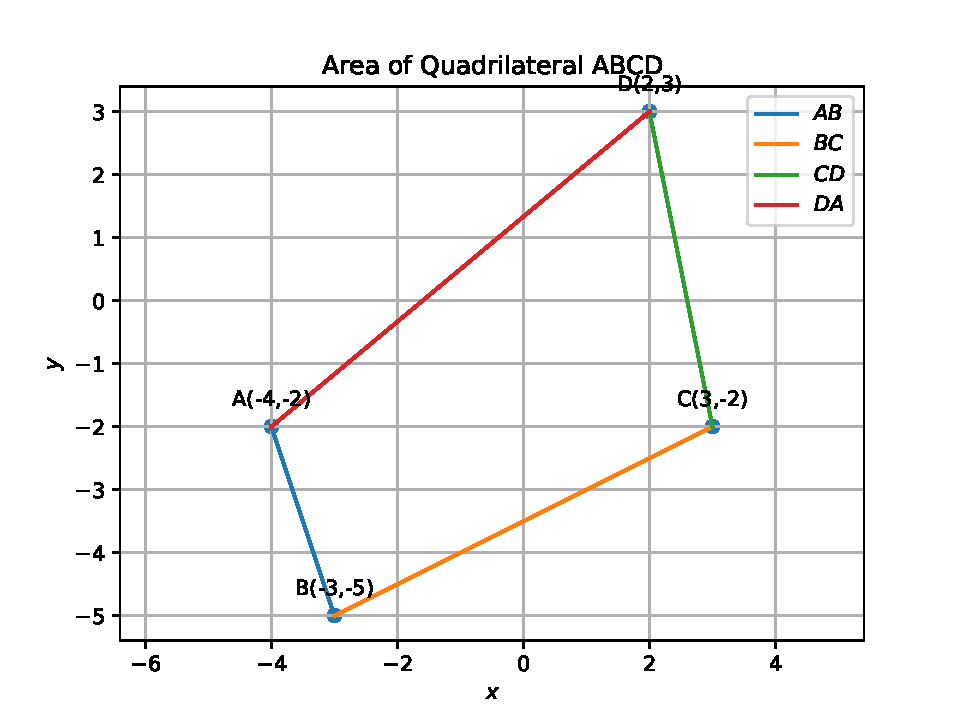
\includegraphics[width=\columnwidth]{chapters/10/7/3/4/figs/fig.pdf}
 \end{center}
\caption{}
\label{fig:chapters/10/7/3/4/Fig1}
\end{figure}


\item Verify that a median of a triangle divides it into two triangles of equal areas for $\triangle ABC$ whose vertices are $\vec{A}(4, -6), \vec{B}(3, 2), \text{ and } \vec{C}(5, 2)$. 
		\label{10/7/3/5}
		\\
\solution
		\iffalse
\documentclass[12pt]{article}
\usepackage{graphicx}
\usepackage[none]{hyphenat}
\usepackage{graphicx}
\usepackage{listings}
\usepackage[english]{babel}
\usepackage{graphicx}
\usepackage{caption} 
\usepackage{booktabs}
\usepackage{array}
\usepackage{amssymb} % for \because
\usepackage{amsmath}   % for having text in math mode
\usepackage{extarrows} % for Row operations arrows
\usepackage{listings}
\usepackage[utf8]{inputenc}
\lstset{
  frame=single,
  breaklines=true
}
\usepackage{hyperref}
  
%Following 2 lines were added to remove the blank page at the beginning
\usepackage{atbegshi}% http://ctan.org/pkg/atbegshi
\AtBeginDocument{\AtBeginShipoutNext{\AtBeginShipoutDiscard}}


%New macro definitions
\newcommand{\mydet}[1]{\ensuremath{\begin{vmatrix}#1\end{vmatrix}}}
\providecommand{\brak}[1]{\ensuremath{\left(#1\right)}}
\newcommand{\solution}{\noindent \textbf{Solution: }}
\newcommand{\myvec}[1]{\ensuremath{\begin{pmatrix}#1\end{pmatrix}}}
\providecommand{\norm}[1]{\left\lVert#1\right\rVert}
\providecommand{\abs}[1]{\left\vert#1\right\vert}
\let\vec\mathbf

\begin{document}

\begin{center}
\title{\textbf{VECTORS}}
\date{\vspace{-5ex}} %Not to print date automatically
\maketitle
\end{center}

\section{10$^{th}$ Maths - EXERCISE-7.3}

\begin{enumerate}
\item That a median of a triangle divides it into two triangles  of equal areas. verify this result for $\triangle ABC$ whose vertices are $\vec{A}(4,-6),\vec{B}(3,-2)\text{ and }\vec{C}(5,2)$.
\end{enumerate}

\section{SOLUTION}
Given points are
\begin{align}
\vec{A}=\myvec{4\\ -6} ,
\vec{B}=\myvec{3\\ -2} ,
\vec{C}=\myvec{5\\ 2}
\end{align}
\fi
The median of the triangle 
\begin{align}
\vec{D}&=\frac{\vec{B}+\vec{C}}{2}\\
&=\myvec{4\\ 0}
\end{align}
Since 
\begin{align}
	\vec{A}- \vec{B} &= \myvec{4\\ -6}-\myvec{3\\ -2}=\myvec{1\\ -4}\label{eq:10/7/3/5/7}\\
	  \vec{A}- \vec{D} &= \myvec{4\\ -6}-\myvec{4\\ 0}=\myvec{0\\ -6}\label{eq:10/7/3/5/8}
  \end{align}
 \begin{align}
  ar(ABD)&=\frac{1}{2} \norm{\brak{\vec{A}-\vec{B}}  \times 
   \brak{\vec{A}- \vec{D}}} \label{eq:10/7/3/5/6} 
   \\
&=\frac{1}{2}\mydet{1 & 0\\-4 & -6}
	       =3	
\end{align}
upon
Substituting from \eqref{eq:10/7/3/5/7} and \eqref{eq:10/7/3/5/8} in \eqref{eq:10/7/3/5/6}.
		Similarly, 
\begin{align}
	\vec{A}- \vec{C} &= \myvec{4\\ -6}-\myvec{5\\ 2}=\myvec{-1\\ -8}\label{eq:10/7/3/5/13} \\
	  \vec{A}- \vec{D} &= \myvec{4\\ -6}-\myvec{4\\ 0}=\myvec{0\\ -6}\label{eq:10/7/3/5/14} 
  \end{align}
  yielding
  \begin{align}
  ar(ACD)&=\frac{1}{2} \norm{\brak{\vec{A}-\vec{C}}  \times 
   \brak{\vec{A}- \vec{D}}} \label{eq:10/7/3/5/12}
   \\
	&=\frac{1}{2}\mydet{-1 & 0\\-8 & -6}= 3
\end{align}
upon substituting from \eqref{eq:10/7/3/5/13} and \eqref{eq:10/7/3/5/14} in \eqref{eq:10/7/3/5/12}.
Thus,
\begin{align}
ar(ABD)=ar(ACD)
\end{align}
See Fig. 
\ref{fig:10/7/3/5/}.
\begin{figure}[h!]
\centering
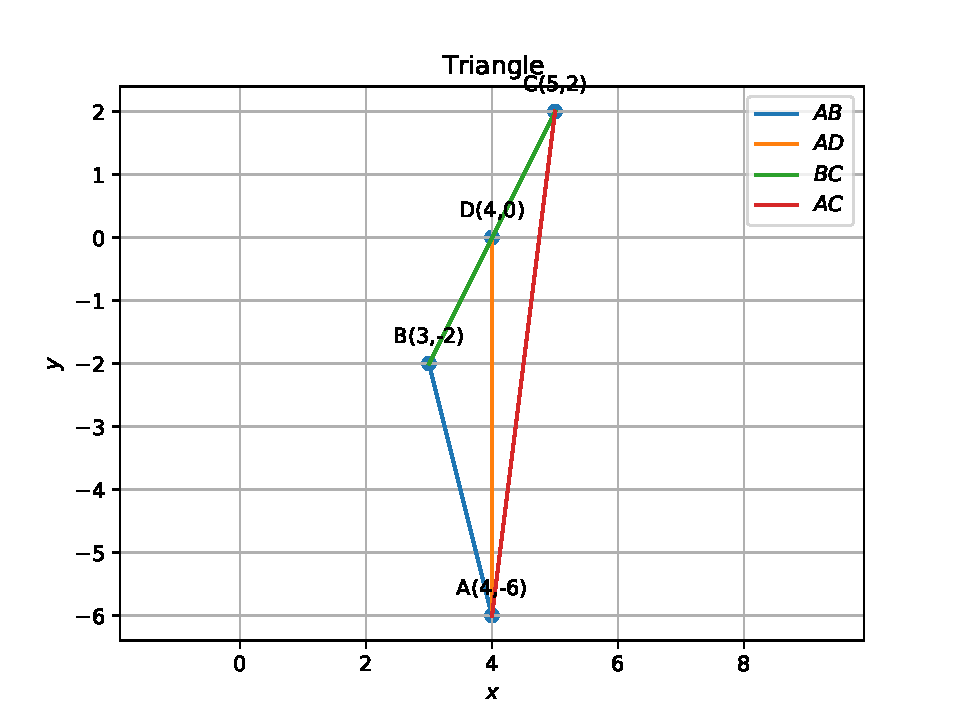
\includegraphics[width=\columnwidth]{chapters/10/7/3/5/figs/fig.pdf}
\caption{}
\label{fig:10/7/3/5/}
\end{figure} 


\item Find the area of region bounded by the triangle whose
	vertices are $(1, 0), (2, 2) \text{ and } (3, 1)$. 
\item Find the area of region bounded by the triangle whose vertices
	are $(– 1, 0), (1, 3) \text{ and } (3, 2)$. 

\item Find the area of the $\triangle ABC$, coordinates of whose vertices are $\vec{A}(2, 0), \vec{B}(4, 5), \text{ and } \vec{C}(6, 3)$.

\end{enumerate}



\section{Vector Product}
\begin{enumerate}[label=\thesection.\arabic*,ref=\thesection.\theenumi]
		\item Find $\abs{\overrightarrow{a}\times\overrightarrow{b}},\text{ if }\overrightarrow{a}=\hat{i}-7\hat{j}+7\hat{k}\text{ and } \overrightarrow{b}=3\hat{i}-2\hat{j}+2\hat{k}$.
\item Find a unit vector perpendicular to each of the vector $\overrightarrow{a}+\overrightarrow{b}\text{ and }\overrightarrow{a}-\overrightarrow{b},\text{ where } \overrightarrow{a}=3\hat{i}+2\hat{j}+2\hat{k}\text{ and } \overrightarrow{b}=\hat{i}+2\hat{j}-2\hat{k}$. 
\item If a unit vector $\overrightarrow{a}$ makes angles $\dfrac{\pi}{3}\text{ with }\hat{i}, \dfrac{\pi}{4}\text{ with }\hat{j}$ and an acute angle $\theta \text{ with }\hat{k},\text{ then find } \theta$ and hence, the components of $\overrightarrow{a}$.
\item Show that $$(\overrightarrow{a}-\overrightarrow{b})\times (\overrightarrow{a}+\overrightarrow{b})=2(\overrightarrow{a}\times \overrightarrow{b})$$
\item Find $\lambda$ and $\mu$ if $(2\hat{i}+6\hat{j}+27\hat{k})\times(\hat{i}+\lambda \hat{j} + \mu \hat{k})=\overrightarrow{0}$.
	\\
		\solution
		\iffalse
\documentclass[12pt]{article}
\usepackage{graphicx}
\usepackage{amsmath}
\usepackage{mathtools}
\usepackage{gensymb}

\newcommand{\mydet}[1]{\ensuremath{\begin{vmatrix}#1\end{vmatrix}}}
\providecommand{\brak}[1]{\ensuremath{\left(#1\right)}}
\providecommand{\norm}[1]{\left\lVert#1\right\rVert}
\newcommand{\solution}{\noindent \textbf{Solution: }}
\newcommand{\myvec}[1]{\ensuremath{\begin{pmatrix}#1\end{pmatrix}}}
\let\vec\mathbf

\begin{document}
\begin{center}
\textbf\large{CHAPTER-10 \\ VECTOR ALGEBRA}

\end{center}
\section*{Excercise 10.4}

Q5.Find $\lambda \text{ and } \mu \text{ if } (2\hat{i}+6\hat{j}+27\hat{k}) \times (\hat{i}+\lambda \hat{j}+\mu \hat{k})=\vec{0}$

\solution
\fi
\begin{align}
	\text{Let } \vec{A} = \myvec{2\\6\\27} \text{ and } \vec{B} = \myvec{1\\ \lambda \\ \mu}\\
\end{align}
The cross product or vector product of $\vec{A},\vec{B}$ is defined as
\begin{align}
	\vec{A} \times \vec{B} = \myvec{\mydet{\vec{A}_{23}&\vec{B}_{23}\\\vec{A}_{31}&\vec{B}_{31}\\\vec{A}_{12}&\vec{B}_{12}}}
\end{align}
Hence
\begin{align}
	\mydet{\vec{A}_{23}&\vec{B}_{23}}&=\mydet{6&\lambda\\27&\mu}=6\mu-27\lambda\\
	\mydet{\vec{A}_{31}&\vec{B}_{31}}&=\mydet{27&\mu\\2&1}=27-2\mu\\
	\mydet{\vec{A}_{12}&\vec{B}_{12}}&=\mydet{2&1\\6&\lambda}=2\lambda-6
\end{align}
Substituting the values
\begin{align}
	\vec{A}\times\vec{B}=\myvec{6\mu-27\lambda\\27-2\mu\\2\lambda-6}
\end{align}
Since
\begin{align}
	\vec{A} \times \vec{B} &= \vec{0},
	\\
	\myvec{6\mu-27\lambda\\27-2\mu\\2\lambda-6}&=\myvec{0\\0\\0},
\end{align}
which can be represented in matrix form as
\begin{align}
	\myvec{2&0\\0&2\\6&-27}\myvec{\mu\\\lambda}&=\myvec{27\\6\\0}.
\end{align}
The augmented matrix is given as
\begin{align}
	\myvec{2 & 0 & \vrule & 27\\0 & 2 & \vrule & 6\\ 6 & -27 & \vrule & 0}
	\xleftrightarrow{R_{3}\rightarrow R_{3}-3R_{1}}  	
	\myvec{2 & 0 & \vrule & 27\\0 & 2 & \vrule & 6\\ 0 & -27 & \vrule & -81}\\
	\xleftrightarrow{R_{3}\rightarrow R_{3}+\frac{27}{2}R_{2}}  	
	\myvec{2 & 0 & \vrule & 27\\0 & 2 & \vrule & 6\\ 0 & 0 & \vrule & 0}
\end{align}
yielding
\begin{align}
	\mu=13.5,
	\lambda=3
\end{align}


\item Given that $\overrightarrow{a} \cdot \overrightarrow{b} = 0$ and $\overrightarrow{a} \times \overrightarrow{b} = \overrightarrow{0}$. What can you conclude about the vectors $\overrightarrow{a} \text{ and }\overrightarrow{b}$?
\item Let the vectors be given as $\overrightarrow{a},\overrightarrow{b},\overrightarrow{c}\text{ be given as }\ a_1 \hat{i}+\ a_2 \hat{j}+\ a_3 \hat{k},\ b_1 \hat{i}+\ b_2 \hat{j}+\ b_3 \hat{k},\ c_1 \hat{i}+\ c_2 \hat{j}+\ c_3 \hat{k}$. Then show that $\overrightarrow{a} \times (\overrightarrow{b} + \overrightarrow{c}) = \overrightarrow{a} \times \overrightarrow{b}+\overrightarrow{a} \times \overrightarrow{c}$.
\item If either $\overrightarrow{a} = \overrightarrow{0}$ or $\overrightarrow{b} = \overrightarrow{0}$, then $\overrightarrow{a} \times \overrightarrow{b} = \overrightarrow{0}$. Is the converse true? Justify your answer with an example.
\item Find the area of the triangle with vertices $A(1, 1, 2)$, $B(2, 3, 5)$, and $C(1, 5, 5)$
\item Find the area of the parallelogram whose adjacent sides are determined by the vectors $\overrightarrow{a}=\hat{i}-\hat{j}+3\hat{k}$ and $\overrightarrow{b}=2\hat{i}-7\hat{j}+\hat{k}$.
\item Let the vectors $\overrightarrow{a}$ and $\overrightarrow{b}$ be such that $|\overrightarrow{a}| = 3$ and $|\overrightarrow{b}| = \dfrac{\sqrt{2}}{3}$, then $\overrightarrow{a} \times \overrightarrow{b}$ is a unit vector, if the angle between $\overrightarrow{a}$ and $\overrightarrow{b}$ is
\begin{enumerate}
\item $\dfrac{\pi}{6}$
\item $\dfrac{\pi}{4}$
\item $\dfrac{\pi}{3}$
\item $\dfrac{\pi}{2}$
\end{enumerate}
\item Area of a rectangle having vertices A, B, C and D with position vectors $ -\hat{i}+ \dfrac{1}{2} \hat{j}+4\hat{k},\hat{i}+ \dfrac{1}{2} \hat{j}+4\hat{k},\hat{i}-\dfrac{1}{2} \hat{j}+4\hat{k}\text{ and }-\hat{i}- \dfrac{1}{2} \hat{j}+4\hat{k}$, respectively is
\begin{enumerate}
\item $\dfrac{1}{2}$
\item 1
\item 2
\item 4
\end{enumerate}
\end{enumerate}


\section{3D Miscellanous}
\begin{enumerate}[label=\thesection.\arabic*,ref=\thesection.\theenumi]
\item Write down a unit vector in XY-plane, making an angle of 30$^{\circ}$ with the positive direction of x-axis.\\
\item Find the scalar components and magnitude of the vector joining the points P($x_1,y_1,z_1 $) and Q ($x_2,y_2,z_2$ ).\\
\item A girl walks 4 km towards west, then she walks 3 km in a direction 30$^{\circ}$ east of north and stops. Determine the girl's displacement from her initial point of departure.\\
	\solution
		\iffalse
\documentclass[12pt]{article}
\usepackage{graphicx}
%\documentclass[journal,12pt,twocolumn]{IEEEtran}
\usepackage[none]{hyphenat}
\usepackage{graphicx}
\usepackage{listings}
\usepackage[english]{babel}
\usepackage{graphicx}
\usepackage{caption}
\usepackage[parfill]{parskip}
\usepackage{hyperref}
\usepackage{booktabs}
\usepackage{gensymb}
%\usepackage{setspace}\doublespacing\pagestyle{plain}
\def\inputGnumericTable{}
\usepackage{color}                                            %%
    \usepackage{array}                                            %%
    \usepackage{longtable}                                        %%
    \usepackage{calc}                                             %%
    \usepackage{multirow}                                         %%
    \usepackage{hhline}                                           %%
    \usepackage{ifthen}
\usepackage{array}
\usepackage{amsmath}   % for having text in math mode
\usepackage{parallel,enumitem}
\usepackage{listings}
\lstset{
language=tex,
frame=single,
breaklines=true
}
 
%Following 2 lines were added to remove the blank page at the beginning
\usepackage{atbegshi}% http://ctan.org/pkg/atbegshi
\AtBeginDocument{\AtBeginShipoutNext{\AtBeginShipoutDiscard}}
%
%New macro definitions
\newcommand{\mydet}[1]{\ensuremath{\begin{vmatrix}#1\end{vmatrix}}}
\providecommand{\brak}[1]{\ensuremath{\left(#1\right)}}
\providecommand{\norm}[1]{\left\lVert#1\right\rVert}
\newcommand{\solution}{\noindent \textbf{Solution: }}
\newcommand{\myvec}[1]{\ensuremath{\begin{pmatrix}#1\end{pmatrix}}}
\let\vec\mathbf
\begin{document}
\begin{center}
\enlargethispage{-4cm}
\title{\textbf{vector Algebra}}
\date{\vspace{-5ex}} %Not to print date automatically
\maketitle
\end{center}
\setcounter{page}{1}
\section*{12$^{th}$ Maths - Chapter 10}
This is Problem-3 from Exercise 10.4
\begin{enumerate}
\item A girl walks $4$ km towards west, then she walk $3$ km in a direction $30\degree$ east of north and stops. Determine the girl's displacement from her initial point of departure.

\solution 
\fi
		Let 
\begin{align}
	\vec{A}=\myvec{0\\0},
			\vec{B} -\vec{A}=\myvec{-4\\0},
	 \vec{C}-\vec{B}=\myvec{3\cos{60\degree}\\3\sin{60\degree}}
&=\myvec{\frac{3}{2}\\ \frac{3\sqrt{3}}{2}}
 \end{align}
 By triangle law of vector addition, 
\begin{align}
	\vec{C}-\vec{A} &= \vec{B}-\vec{A}+\vec{C}-\vec{B}\\
 &=\myvec{-4\\0}+\myvec{\frac{3}{2}\\[2pt] \frac{3\sqrt{3}}{2}}
=\myvec{\frac{-5}{2}\\[2pt] \frac{3\sqrt{3}}{2}}
\end{align}
which is the girl's displacement from her initial point of departure 
See Fig. 
\ref{fig:chapters/12/10/5/3Fig1}.
\begin{figure}[!h] 
 \begin{center} 
 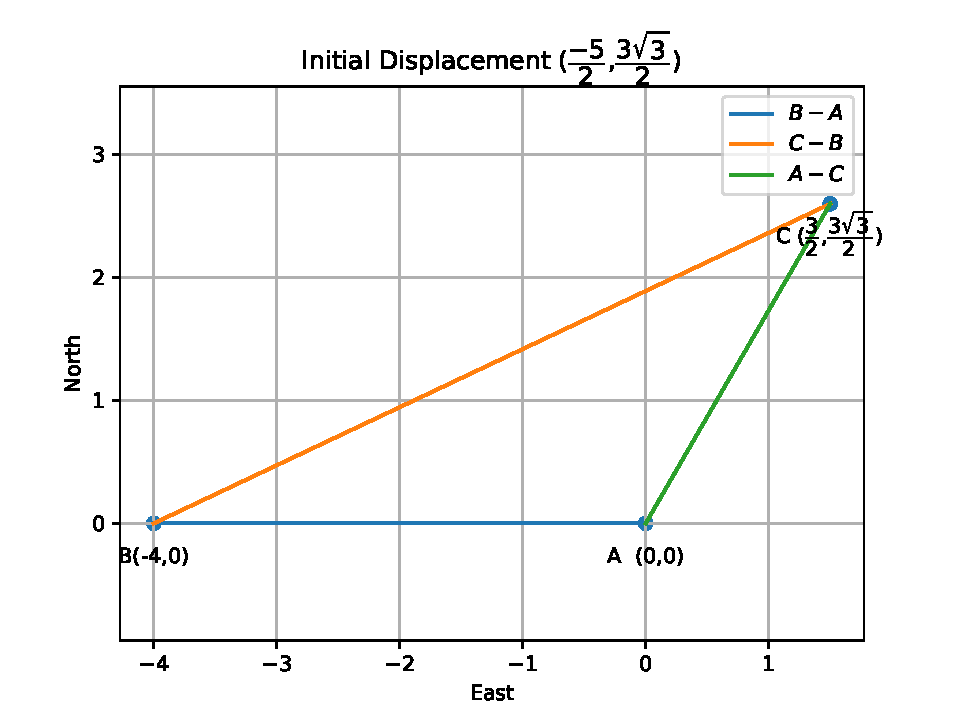
\includegraphics[width=\columnwidth]{chapters/12/10/5/3/figs/fig.pdf} 
 \end{center} 
\caption{} 
\label{fig:chapters/12/10/5/3Fig1} 
\end{figure}

\item If $\vec{a}=\vec{b}+\vec{c}$, then is it true that $|\vec{a}|=|\vec{b}|+|\vec{c}|$? Justify your answer.\\
	\solution
		\iffalse
\documentclass[journal,12pt,twocolumn]{IEEEtran}
\usepackage{graphicx}
\graphicspath{{./figs/}}{}
\usepackage{amsmath,amssymb,amsfonts,amsthm}
\newcommand{\myvec}[1]{\ensuremath{\begin{pmatrix}#1\end{pmatrix}}}
\providecommand{\norm}[1]{\lVert#1\rVert}
\usepackage{listings}
\usepackage{watermark}
\usepackage{titlesec}
\usepackage{caption}
\newcommand{\mydet}[1]{\ensuremath{\begin{vmatrix}#1\end{vmatrix}}}
\let\vec\mathbf
\lstset{
frame=single, 
breaklines=true,
columns=fullflexible
}
\thiswatermark{\centering \put(0,-105.0){
\includegraphics[scale=0.15]{/sdcard/IITH/vectors/12.10.5.4/figs/logo.png}} }
\title{\mytitle}
\title{
Assignment - 12.10.5.4
}
\author{Surajit Sarkar}
\begin{document}
\maketitle
\tableofcontents
\bigskip
\section{\textbf{Problem}}
if $\vec{a}=\vec{b}+\vec{c}$, then is true that $|\vec{a}|=|\vec{b}|+|\vec{c}|$?
Justify your answer .
\section{\textbf{Solution}}
Given
\begin{align}
    \vec{a}=\vec{b}+\vec{c}
\end{align}
\fi
Let
\begin{align}
    \vec{b}=\myvec{1\\2\\3},\vec{c}=\myvec{2\\-1\\-2}
\end{align}
Then
\begin{align}
	\vec{a}&=\vec{b}+\vec{c}
    =\myvec{3\\1\\1}
    \\
	\implies
    \norm{\vec{a}}
    &=\sqrt{11},\,
    \norm{\vec{b}}    =\sqrt{14},\,
    \norm{\vec{c}}
    =3.
\end{align}
Thus
\begin{align}
	\norm{\vec{a}}\ne\norm{\vec{b}}+\norm{\vec{c}}
\end{align}


\item Find the value of x for which $x(\hat{i}+\hat{j}+\hat{k})$ is a unit vector.\\
	\solution
		\iffalse
\documentclass[12pt]{article}
\usepackage{graphicx}
\usepackage[none]{hyphenat}
\usepackage{graphicx}
\usepackage{listings}
\usepackage[english]{babel}
\usepackage{graphicx}
\usepackage{caption} 
\usepackage{booktabs}
\usepackage{array}
\usepackage{amssymb} % for \because
\usepackage{amsmath}   % for having text in math mode
\usepackage{extarrows} % for Row operations arrows
\usepackage{listings}
\lstset{
  frame=single,
  breaklines=true
}
\usepackage{hyperref}
  
%Following 2 lines were added to remove the blank page at the beginning
\usepackage{atbegshi}% http://ctan.org/pkg/atbegshi
\AtBeginDocument{\AtBeginShipoutNext{\AtBeginShipoutDiscard}}


%New macro definitions
\newcommand{\mydet}[1]{\ensuremath{\begin{vmatrix}#1\end{vmatrix}}}
\providecommand{\brak}[1]{\ensuremath{\left(#1\right)}}
\providecommand{\norm}[1]{\left\lVert#1\right\rVert}
\newcommand{\solution}{\noindent \textbf{Solution: }}
\newcommand{\myvec}[1]{\ensuremath{\begin{pmatrix}#1\end{pmatrix}}}
\providecommand{\abs}[1]{\left\vert#1\right\vert}
\let\vec\mathbf

\begin{document}

\begin{center}
\title{\textbf{Equation  of Unit Vector}}
\date{\vspace{-5ex}} %Not to print date automatically
\maketitle
\end{center}
\setcounter{page}{1}
\section{12$^{th}$ Maths - Chapter 10}
\textbf{This is Problem-5 from Exercise 5.5}
\begin{enumerate}
\item Find the value of $x$ for which $x(\hat{i}+\hat{j}+\hat{k})$ is a unit vector
\section{Solution}
\solution
\fi
Let
\begin{align} 
\vec{x}&=x\myvec{1\\1\\1}
\implies
\norm{\vec{x}}=1
\\
\implies 
x\sqrt{3}&=1,\,
	\text{or, }x=\frac{1}{\sqrt{3}}
\end{align}   

\item Find a vector of magnitude 5 units, and parallel to the resultant of the vectors $\vec{a}=2\hat{i}+3\hat{j}-\hat{k}$ and $\vec{b}=\hat{i}-2\hat{j}+\hat{k}$.\\
\item If $\vec{a}=\hat{i}+\hat{j}+\hat{k}$,$\vec{b}=2\hat{i}-\hat{j}+3\hat{k}$ and $\vec{c}=\hat{i}-2\hat{j}+\hat{k}$, find a unit vector parallel to the vector $2\vec{a}-\vec{b}+3\vec{c}$.\\
	\solution
		\iffalse
\documentclass[10pt]{article}
\usepackage{graphicx}
\usepackage[none]{hyphenat}
\usepackage{graphicx}
\usepackage{listings}
\usepackage[english]{babel}
\usepackage{siunitx}
\usepackage{graphicx}
\usepackage{caption} 
\usepackage{booktabs}
\usepackage{array}
\usepackage{amssymb} % for \because
\usepackage{amsmath}   % for having text in math mode
\usepackage{extarrows} % for Row operations arrows
\usepackage{listings}
\usepackage[utf8]{inputenc}
\lstset{
  frame=single,
  breaklines=true
}
\usepackage{hyperref}
  
%Following 2 lines were added to remove the blank page at the beginning
\usepackage{atbegshi}% http://ctan.org/pkg/atbegshi
\AtBeginDocument{\AtBeginShipoutNext{\AtBeginShipoutDiscard}}


%New macro definitions
\newcommand{\mydet}[1]{\ensuremath{\begin{vmatrix}#1\end{vmatrix}}}
\providecommand{\brak}[1]{\ensuremath{\left(#1\right)}}
\newcommand{\solution}{\noindent \textbf{Solution: }}
\newcommand{\myvec}[1]{\ensuremath{\begin{pmatrix}#1\end{pmatrix}}}
\providecommand{\norm}[1]{\left\lVert#1\right\rVert}
\providecommand{\abs}[1]{\left\vert#1\right\vert}
\let\vec\mathbf{}
\begin{document}

\begin{center}
\title{\textbf{Vector Algebra}}
\date{\vspace{-5ex}} %Not to print date automatically
\maketitle
\end{center}

\section{12$^{th}$ Maths - Chapter 10}
This is Problem 7 from Exercise-10.5
\begin{enumerate}

\item If $\overrightarrow{a}=\hat{i}+\hat{j}+\hat{k}$,$\overrightarrow{b}=2\hat{i}-\hat{j}+3\hat{k}$ and $\overrightarrow{c}=\hat{i}-2\hat{j}+\hat{k}$, find a unit vector parallel to the vector $2\overrightarrow{a}-\overrightarrow{b}+3\overrightarrow{c}$.\\  

\solution
Given Vectors
\fi

\begin{align}
	\vec{u}=2\vec{a}-\vec{b}+3\vec{c}=\myvec{3\\-3\\2}
\implies
\hat{\vec{u}}=\frac{\vec{u}}{\norm{\vec{u}}}
=\frac{1}{\sqrt{22}}\myvec{3\\-3\\2}
\end{align}


\item Show that the points A (1, -2, -8), B (5, 0, -2) and C (11, 3, 7) are collinear, and find the ratio in which B divides AC.\\
\item Find the position vector of a point R which divides the line joining two points P and Q whose position vectors are $(2\vec{a}+\vec{b})$ and $(\vec{a}-3\vec{b})$
externally in the ratio 1 : 2. Also, show that P is the mid point of the line segment RQ.\\
	\solution
%		\iffalse
\documentclass[10pt]{article}
\usepackage{graphicx}
\usepackage[none]{hyphenat}
\usepackage{graphicx}
\usepackage{listings}
\usepackage[english]{babel}
\usepackage{siunitx}
\usepackage{graphicx}
\usepackage{caption} 
\usepackage{booktabs}
\usepackage{array}
\usepackage{amssymb} % for \because
\usepackage{amsmath}   % for having text in math mode
\usepackage{extarrows} % for Row operations arrows
\usepackage{listings}
\usepackage[utf8]{inputenc}
\lstset{
  frame=single,
  breaklines=true
}
\usepackage{hyperref}
  
%Following 2 lines were added to remove the blank page at the beginning
\usepackage{atbegshi}% http://ctan.org/pkg/atbegshi
\AtBeginDocument{\AtBeginShipoutNext{\AtBeginShipoutDiscard}}


%New macro definitions
\newcommand{\mydet}[1]{\ensuremath{\begin{vmatrix}#1\end{vmatrix}}}
\providecommand{\brak}[1]{\ensuremath{\left(#1\right)}}
\newcommand{\solution}{\noindent \textbf{Solution: }}
\newcommand{\myvec}[1]{\ensuremath{\begin{pmatrix}#1\end{pmatrix}}}
\providecommand{\norm}[1]{\left\lVert#1\right\rVert}
\providecommand{\abs}[1]{\left\vert#1\right\vert}
\let\vec\mathbf{}
\begin{document}

\begin{center}
\title{\textbf{VECTORS}}
\date{\vspace{-5ex}} %Not to print date automatically
\maketitle
\end{center}

\section*{12$^{th}$ Maths - EXERCISE-10.5}

Find the position vector of a point R which divides the line joining two points  P and Q whose position vectors are P = $\myvec{2\\ 1 \\}$ and Q = $\myvec{ 1\\-3\\ }$  externally in the ratio 1:2.Also show that P is the midpoint of the linesegment RQ.

\solution

\begin{align}
\vec{P} = \myvec{ 2\\1\\} 
 \label{eq1} \\
 \vec{Q} = \myvec{ 1\\-3\\}
\end{align}
\fi
When $\vec{R}$ divides line segment joining $\vec{P}$ and $\vec{Q}$ externally,
\begin{align}
\vec{R} &= \frac{\vec{Q} -2\vec{P}}{-1} 
= \myvec{3\\5}
\end{align}
Also,
\begin{align}
\frac{ (\vec{R} + \vec{Q})}{2}
=\myvec{2\\1} =\vec{P}
\end{align}
See Fig. 
\ref{fig:chapters/12/10/5/9/Figure1}.
\begin{figure}[!h]
	\begin{center}
		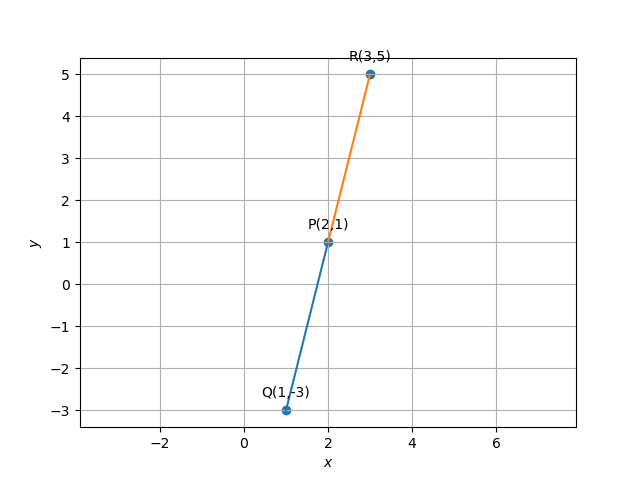
\includegraphics[width=\columnwidth]{chapters/12/10/5/9/figs/line.png}
	\end{center}
\caption{}
\label{fig:chapters/12/10/5/9/Figure1}
\end{figure}

\item The two adjacent sides of a parallelogram are 
$2\hat{i}-4\hat{j}+5\hat{k}$  and  $\hat{i}-2\hat{j}-3\hat{k}$.
Find the unit vector parallel to its diagonal. Also, find its area.\\
	\solution
		\iffalse
\documentclass[journal,12pt,twocolumn]{IEEEtran}
\usepackage{setspace}
\usepackage{gensymb}
\usepackage{xcolor}
\usepackage{caption}
\singlespacing
\usepackage{siunitx}
\usepackage[cmex10]{amsmath}
\usepackage{mathtools}
\usepackage{hyperref}
\usepackage{amsthm}
\usepackage{mathrsfs}
\usepackage{txfonts}
\usepackage{stfloats}
\usepackage{cite}
\usepackage{cases}
\usepackage{subfig}
\usepackage{longtable}
\usepackage{multirow}
\usepackage{enumitem}
\usepackage{bm}
\usepackage{mathtools}
\usepackage{listings}
\usepackage{tikz}
\usetikzlibrary{shapes,arrows,positioning}
\usepackage{circuitikz}
\renewcommand{\vec}[1]{\boldsymbol{\mathbf{#1}}}
\DeclareMathOperator*{\Res}{Res}
\renewcommand\thesection{\arabic{section}}
\renewcommand\thesubsection{\thesection.\arabic{subsection}}
\renewcommand\thesubsubsection{\thesubsection.\arabic{subsubsection}}

\renewcommand\thesectiondis{\arabic{section}}
\renewcommand\thesubsectiondis{\thesectiondis.\arabic{subsection}}
\renewcommand\thesubsubsectiondis{\thesubsectiondis.\arabic{subsubsection}}
\hyphenation{op-tical net-works semi-conduc-tor}

\lstset{
language=Python,
frame=single, 
breaklines=true,
columns=fullflexible
}
\begin{document}
\theoremstyle{definition}
\newtheorem{theorem}{Theorem}[section]
\newtheorem{problem}{Problem}
\newtheorem{proposition}{Proposition}[section]
\newtheorem{lemma}{Lemma}[section]
\newtheorem{corollary}[theorem]{Corollary}
\newtheorem{example}{Example}[section]
\newtheorem{definition}{Definition}[section]
\newcommand{\BEQA}{\begin{eqnarray}}
        \newcommand{\EEQA}{\end{eqnarray}}
\newcommand{\define}{\stackrel{\triangle}{=}}
\newcommand{\myvec}[1]{\ensuremath{\begin{pmatrix}#1\end{pmatrix}}}
\newcommand{\mydet}[1]{\ensuremath{\begin{vmatrix}#1\end{vmatrix}}}
\bibliographystyle{IEEEtran}
\providecommand{\nCr}[2]{\,^{#1}C_{#2}} % nCr
\providecommand{\nPr}[2]{\,^{#1}P_{#2}} % nPr
\providecommand{\mbf}{\mathbf}
\providecommand{\pr}[1]{\ensuremath{\Pr\left(#1\right)}}
\providecommand{\qfunc}[1]{\ensuremath{Q\left(#1\right)}}
\providecommand{\sbrak}[1]{\ensuremath{{}\left[#1\right]}}
\providecommand{\lsbrak}[1]{\ensuremath{{}\left[#1\right.}}
\providecommand{\rsbrak}[1]{\ensuremath{{}\left.#1\right]}}
\providecommand{\brak}[1]{\ensuremath{\left(#1\right)}}
\providecommand{\lbrak}[1]{\ensuremath{\left(#1\right.}}
\providecommand{\rbrak}[1]{\ensuremath{\left.#1\right)}}
\providecommand{\cbrak}[1]{\ensuremath{\left\{#1\right\}}}
\providecommand{\lcbrak}[1]{\ensuremath{\left\{#1\right.}}
\providecommand{\rcbrak}[1]{\ensuremath{\left.#1\right\}}}
\theoremstyle{remark}
\newtheorem{rem}{Remark}
\newcommand{\sgn}{\mathop{\mathrm{sgn}}}
\newcommand{\rect}{\mathop{\mathrm{rect}}}
\newcommand{\sinc}{\mathop{\mathrm{sinc}}}
\providecommand{\abs}[1]{\left\vert#1\right\vert}
\providecommand{\res}[1]{\Res\displaylimits_{#1}}
\providecommand{\norm}[1]{\lVert#1\rVert}
\providecommand{\mtx}[1]{\mathbf{#1}}
\providecommand{\mean}[1]{E\left[ #1 \right]}
\providecommand{\fourier}{\overset{\mathcal{F}}{ \rightleftharpoons}}
\providecommand{\ztrans}{\overset{\mathcal{Z}}{ \rightleftharpoons}}
\providecommand{\system}[1]{\overset{\mathcal{#1}}{ \longleftrightarrow}}
\newcommand{\solution}{\noindent \textbf{Solution: }}
\providecommand{\dec}[2]{\ensuremath{\overset{#1}{\underset{#2}{\gtrless}}}}
\let\StandardTheFigure\thefigure
\def\putbox#1#2#3{\makebox[0in][l]{\makebox[#1][l]{}\raisebox{\baselineskip}[0in][0in]{\raisebox{#2}[0in][0in]{#3}}}}
\def\rightbox#1{\makebox[0in][r]{#1}}
\def\centbox#1{\makebox[0in]{#1}}
\def\topbox#1{\raisebox{-\baselineskip}[0in][0in]{#1}}
\def\midbox#1{\raisebox{-0.5\baselineskip}[0in][0in]{#1}}

\vspace{3cm}
\title{12.10.5.10}
\author{Lokesh Surana}
\maketitle
\section*{Class 12, Chapter 10, Exercise 5.10}

Q.10. The two adjacent sides of a parallelogram are  ${2}\hat{i} -  {4}\hat{j} + {5}\hat{k}$ and ${1}\hat{i} -  {2}\hat{j} - {3}\hat{k}$.
Find the unit vector parallel to its diagonal. Also, find its area.

\solution 
\fi
Let the sides of the parallelogram be 
\begin{align}
\vec{a} = \myvec{2\\-4\\5}, \, \vec{b} = \myvec{1\\-2\\-3}.
\end{align}
The diagonals of the parallelogram are given by
\begin{align}
	\vec{D}_1 &= \vec{a} + \vec{b} = \myvec{3 \\-6\\2} \\
	\vec{D}_2 &= \vec{a} - \vec{b} = \myvec{1 \\-2\\8}
\end{align}
The unit vectors parallel to the diagonals are then given by
\begin{align}
	\hat{\vec{D}_1} &= \frac{\vec{D}_1}{\norm{\vec{D}_1}}  = \myvec{\frac{3}{\sqrt{45}}\\-\frac{6}{\sqrt{45}}\\\frac{2}{\sqrt{45}}} \\
    \hat{\vec{D}_2} &= \frac{\vec{D}_2}{\norm{\vec{D}_2}}  = \myvec{\frac{1}{\sqrt{69}}\\-\frac{2}{\sqrt{69}}\\\frac{8}{\sqrt{69}}}
\end{align}
%
Since
\begin{align}
    \vec{a}\times\vec{b}=\myvec{22 \\-11\\0},
\end{align}
he area of the parallelogram is given by
\begin{align}
    \norm{\vec{a}\times\vec{b}}  = \sqrt{605}
\end{align}


\item Show that the direction cosines of a vector equally inclined to the axes OX, OY and OZ are \textpm $\sbrak{\frac{1}{\sqrt{3}},\frac{1}{\sqrt{3}},\frac{1}{\sqrt{3}}}$.\\
	\solution
		\iffalse
\documentclass[journal,12pt,twocolumn]{IEEEtran}
%
\usepackage{setspace}
\usepackage{gensymb}
%\doublespacing
\singlespacing

%\usepackage{graphicx}
%\usepackage{amssymb}
%\usepackage{relsize}
\usepackage[cmex10]{amsmath}
%\usepackage{amsthm}
%\interdisplaylinepenalty=2500
%\savesymbol{iint}
%\usepackage{txfonts}
%\restoresymbol{TXF}{iint}
%\usepackage{wasysym}
\usepackage{amsthm}
%\usepackage{iithtlc}
\usepackage{mathrsfs}
\usepackage{txfonts}
\usepackage{stfloats}
\usepackage{bm}
\usepackage{cite}
\usepackage{cases}
\usepackage{subfig}
%\usepackage{xtab}
\usepackage{longtable}
\usepackage{multirow}
%\usepackage{algorithm}
%\usepackage{algpseudocode}
\usepackage{enumitem}
\usepackage{mathtools}
\usepackage{steinmetz}
\usepackage{tikz}
\usepackage{circuitikz}
\usepackage{verbatim}
\usepackage{tfrupee}
\usepackage[breaklinks=true]{hyperref}
%\usepackage{stmaryrd}
\usepackage{tkz-euclide} % loads  TikZ and tkz-base
%\usetkzobj{all}
\usetikzlibrary{calc,math}
\usepackage{listings}
    \usepackage{color}                                            %%
    \usepackage{array}                                            %%
    \usepackage{longtable}                                        %%
    \usepackage{calc}                                             %%
    \usepackage{multirow}                                         %%
    \usepackage{hhline}                                           %%
    \usepackage{ifthen}                                           %%
  %optionally (for landscape tables embedded in another document): %%
    \usepackage{lscape}     
\usepackage{multicol}
\usepackage{chngcntr}
%\usepackage{enumerate}

%\usepackage{wasysym}
%\newcounter{MYtempeqncnt}
\DeclareMathOperator*{\Res}{Res}
%\renewcommand{\baselinestretch}{2}
\renewcommand\thesection{\arabic{section}}
\renewcommand\thesubsection{\thesection.\arabic{subsection}}
\renewcommand\thesubsubsection{\thesubsection.\arabic{subsubsection}}

\renewcommand\thesectiondis{\arabic{section}}
\renewcommand\thesubsectiondis{\thesectiondis.\arabic{subsection}}
\renewcommand\thesubsubsectiondis{\thesubsectiondis.\arabic{subsubsection}}

% correct bad hyphenation here
\hyphenation{op-tical net-works semi-conduc-tor}
\def\inputGnumericTable{}                                 %%

\lstset{
%language=C,
frame=single, 
breaklines=true,
columns=fullflexible
}
%\lstset{
%language=tex,
%frame=single, 
%breaklines=true
%}

\begin{document}
%


\newtheorem{theorem}{Theorem}[section]
\newtheorem{problem}{Problem}
\newtheorem{proposition}{Proposition}[section]
\newtheorem{lemma}{Lemma}[section]
\newtheorem{corollary}[theorem]{Corollary}
\newtheorem{example}{Example}[section]
\newtheorem{definition}[problem]{Definition}
%\newtheorem{thm}{Theorem}[section] 
%\newtheorem{defn}[thm]{Definition}
%\newtheorem{algorithm}{Algorithm}[section]
%\newtheorem{cor}{Corollary}
\newcommand{\BEQA}{\begin{eqnarray}}
\newcommand{\EEQA}{\end{eqnarray}}
\newcommand{\define}{\stackrel{\triangle}{=}}

\bibliographystyle{IEEEtran}
%\bibliographystyle{ieeetr}


\providecommand{\mbf}{\mathbf}
\providecommand{\pr}[1]{\ensuremath{\Pr\left(#1\right)}}
\providecommand{\qfunc}[1]{\ensuremath{Q\left(#1\right)}}
\providecommand{\sbrak}[1]{\ensuremath{{}\left[#1\right]}}
\providecommand{\lsbrak}[1]{\ensuremath{{}\left[#1\right.}}
\providecommand{\rsbrak}[1]{\ensuremath{{}\left.#1\right]}}
\providecommand{\brak}[1]{\ensuremath{\left(#1\right)}}
\providecommand{\lbrak}[1]{\ensuremath{\left(#1\right.}}
\providecommand{\rbrak}[1]{\ensuremath{\left.#1\right)}}
\providecommand{\cbrak}[1]{\ensuremath{\left\{#1\right\}}}
\providecommand{\lcbrak}[1]{\ensuremath{\left\{#1\right.}}
\providecommand{\rcbrak}[1]{\ensuremath{\left.#1\right\}}}
\theoremstyle{remark}
\newtheorem{rem}{Remark}
\newcommand{\sgn}{\mathop{\mathrm{sgn}}}
\providecommand{\abs}[1]{\left\vert#1\right\vert}
\providecommand{\res}[1]{\Res\displaylimits_{#1}} 
\providecommand{\norm}[1]{\left\lVert#1\right\rVert}
%\providecommand{\norm}[1]{\lVert#1\rVert}
\providecommand{\mtx}[1]{\mathbf{#1}}
\providecommand{\mean}[1]{E\left[ #1 \right]}
\providecommand{\fourier}{\overset{\mathcal{F}}{ \rightleftharpoons}}
%\providecommand{\hilbert}{\overset{\mathcal{H}}{ \rightleftharpoons}}
\providecommand{\system}{\overset{\mathcal{H}}{ \longleftrightarrow}}
	%\newcommand{\solution}[2]{\textbf{Solution:}{#1}}
\newcommand{\solution}{\noindent \textbf{Solution: }}
\newcommand{\cosec}{\,\text{cosec}\,}
\providecommand{\dec}[2]{\ensuremath{\overset{#1}{\underset{#2}{\gtrless}}}}
\newcommand{\myvec}[1]{\ensuremath{\begin{pmatrix}#1\end{pmatrix}}}
\newcommand{\mydet}[1]{\ensuremath{\begin{vmatrix}#1\end{vmatrix}}}
%\numberwithin{equation}{section}
\numberwithin{equation}{subsection}
%\numberwithin{problem}{section}
%\numberwithin{definition}{section}
\makeatletter
\@addtoreset{figure}{problem}
\makeatother

\let\StandardTheFigure\thefigure
\let\vec\mathbf
%\renewcommand{\thefigure}{\theproblem.\arabic{figure}}
\renewcommand{\thefigure}{\theproblem}
%\setlist[enumerate,1]{before=\renewcommand\theequation{\theenumi.\arabic{equation}}
%\counterwithin{equation}{enumi}


%\renewcommand{\theequation}{\arabic{subsection}.\arabic{equation}}

\def\putbox#1#2#3{\makebox[0in][l]{\makebox[#1][l]{}\raisebox{\baselineskip}[0in][0in]{\raisebox{#2}[0in][0in]{#3}}}}
     \def\rightbox#1{\makebox[0in][r]{#1}}
     \def\centbox#1{\makebox[0in]{#1}}
     \def\topbox#1{\raisebox{-\baselineskip}[0in][0in]{#1}}
     \def\midbox#1{\raisebox{-0.5\baselineskip}[0in][0in]{#1}}

\vspace{3cm}


\title{Question: 12.10.5.11}
\author{Nikam Pratik Balasaheb (EE21BTECH11037)}





% make the title area
\maketitle

\newpage

%\tableofcontents

\bigskip

\renewcommand{\thefigure}{\theenumi}
\renewcommand{\thetable}{\theenumi}
%\renewcommand{\theequation}{\theenumi}

\section{Problem}
Show that direction cosines of a vector equally inclined to axes $ \vec{OX}, \vec{OY}$ and $\vec{OZ}$ are $\pm \myvec{\frac{1}{\sqrt{3}} \\[1pt] \frac{1}{\sqrt{3}} \\[1pt] \frac{1}{\sqrt{3}}} $
\section{Solution}
The vector is equally inclined to the axes $\vec{OX}$, $\vec{OY}$ and $\vec{OZ}$. Let the angle be $\theta$.
\fi

The direction vector can be expressed in terms of the direction cosines as 
\begin{align}
\vec{m}  = \myvec{\cos{\theta} \\ \cos{\theta} \\ \cos{\theta} }
\end{align}
Since 
\begin{align}
\norm{\vec{m}} = 1,
\abs{\sqrt{3} \cos{\theta}} =1 \implies
\cos{\theta} = \pm \frac{1}{\sqrt{3}}
\end{align}


\item Let $\vec{a}=\hat{i}+4\hat{j}+2\hat{k}$,$\vec{b}=3\hat{i}-2\hat{j}+7\hat{k}$ and $\vec{c}=2\hat{i}-\hat{j}+4\hat{k}$.Find a vector $\vec{d}$ which is perpendicular to both $\vec{a}$ and $\vec{b}$,and $\vec{c}.\vec{d}$=15.\\
	\solution
		\iffalse
\documentclass[journal,12pt,twocolumn]{IEEEtran}
\usepackage{setspace}
\usepackage{gensymb}
\singlespacing
\usepackage[cmex10]{amsmath}
\usepackage{amsthm}
\usepackage{mathrsfs}
\usepackage{txfonts}
\usepackage{stfloats}
\usepackage{bm}
\usepackage{cite}
\usepackage{cases}
\usepackage{subfig}
\usepackage{longtable}
\usepackage{multirow}
\usepackage{enumitem}
\usepackage{mathtools}
\usepackage{steinmetz}
\usepackage{tikz}
\usepackage{circuitikz}
\usepackage{verbatim}
\usepackage{tfrupee}
\usepackage[breaklinks=true]{hyperref}
\usepackage{tkz-euclide}
\usetikzlibrary{calc,math}
\usepackage{listings}
    \usepackage{color}                                            %%
    \usepackage{array}                                            %%
    \usepackage{longtable}                                        %%
    \usepackage{calc}                                             %%
    \usepackage{multirow}                                         %%
    \usepackage{hhline}                                           %%
    \usepackage{ifthen}                                           %%
  %optionally (for landscape tables embedded in another document): %%
    \usepackage{lscape}     
\usepackage{multicol}
\usepackage{chngcntr}
\DeclareMathOperator*{\Res}{Res}
\renewcommand\thesection{\arabic{section}}
\renewcommand\thesubsection{\thesection.\arabic{subsection}}
\renewcommand\thesubsubsection{\thesubsection.\arabic{subsubsection}}

\renewcommand\thesectiondis{\arabic{section}}
\renewcommand\thesubsectiondis{\thesectiondis.\arabic{subsection}}
\renewcommand\thesubsubsectiondis{\thesubsectiondis.\arabic{subsubsection}}

% correct bad hyphenation here
\hyphenation{op-tical net-works semi-conduc-tor}
\def\inputGnumericTable{}                                 %%

\lstset{
frame=single, 
breaklines=true,
columns=fullflexible
}

\begin{document}


\newtheorem{theorem}{Theorem}[section]
\newtheorem{problem}{Problem}
\newtheorem{proposition}{Proposition}[section]
\newtheorem{lemma}{Lemma}[section]
\newtheorem{corollary}[theorem]{Corollary}
\newtheorem{example}{Example}[section]
\newtheorem{definition}[problem]{Definition}
\newcommand{\BEQA}{\begin{eqnarray}}
\newcommand{\EEQA}{\end{eqnarray}}
\newcommand{\define}{\stackrel{\triangle}{=}}

\bibliographystyle{IEEEtran}
\providecommand{\mbf}{\mathbf}
\providecommand{\pr}[1]{\ensuremath{\Pr\left(#1\right)}}
\providecommand{\qfunc}[1]{\ensuremath{Q\left(#1\right)}}
\providecommand{\sbrak}[1]{\ensuremath{{}\left[#1\right]}}
\providecommand{\lsbrak}[1]{\ensuremath{{}\left[#1\right.}}
\providecommand{\rsbrak}[1]{\ensuremath{{}\left.#1\right]}}
\providecommand{\brak}[1]{\ensuremath{\left(#1\right)}}
\providecommand{\lbrak}[1]{\ensuremath{\left(#1\right.}}
\providecommand{\rbrak}[1]{\ensuremath{\left.#1\right)}}
\providecommand{\cbrak}[1]{\ensuremath{\left\{#1\right\}}}
\providecommand{\lcbrak}[1]{\ensuremath{\left\{#1\right.}}
\providecommand{\rcbrak}[1]{\ensuremath{\left.#1\right\}}}
\theoremstyle{remark}
\newtheorem{rem}{Remark}
\newcommand{\sgn}{\mathop{\mathrm{sgn}}}
\providecommand{\abs}[1]{\left\vert#1\right\vert}
\providecommand{\res}[1]{\Res\displaylimits_{#1}} 
\providecommand{\norm}[1]{\left\lVert#1\right\rVert}
\providecommand{\mtx}[1]{\mathbf{#1}}
\providecommand{\mean}[1]{E\left[ #1 \right]}
\providecommand{\fourier}{\overset{\mathcal{F}}{ \rightleftharpoons}}
\providecommand{\system}{\overset{\mathcal{H}}{ \longleftrightarrow}}
\newcommand{\solution}{\noindent \textbf{Solution: }}
\newcommand{\cosec}{\,\text{cosec}\,}
\providecommand{\dec}[2]{\ensuremath{\overset{#1}{\underset{#2}{\gtrless}}}}
\newcommand{\myvec}[1]{\ensuremath{\begin{pmatrix}#1\end{pmatrix}}}
\newcommand{\mydet}[1]{\ensuremath{\begin{vmatrix}#1\end{vmatrix}}}
\numberwithin{equation}{subsection}
\makeatletter
\@addtoreset{figure}{problem}
\makeatother

\let\StandardTheFigure\thefigure
\let\vec\mathbf
\renewcommand{\thefigure}{\theproblem}



\def\putbox#1#2#3{\makebox[0in][l]{\makebox[#1][l]{}\raisebox{\baselineskip}[0in][0in]{\raisebox{#2}[0in][0in]{#3}}}}
     \def\rightbox#1{\makebox[0in][r]{#1}}
     \def\centbox#1{\makebox[0in]{#1}}
     \def\topbox#1{\raisebox{-\baselineskip}[0in][0in]{#1}}
     \def\midbox#1{\raisebox{-0.5\baselineskip}[0in][0in]{#1}}

\vspace{3cm}


\title{Assignment 1}
\author{Jaswanth Chowdary Madala}





% make the title area
\maketitle

\newpage

%\tableofcontents

\bigskip

\renewcommand{\thefigure}{\theenumi}
\renewcommand{\thetable}{\theenumi}

\begin{enumerate}
\item Let 	$\overrightarrow{a} = \hat{i}+4\hat{j}+2\hat{k}$, $\overrightarrow{b} = 3\hat{i}-2\hat{j}+7\hat{k}$ and 	$\overrightarrow{c} = 2\hat{i}-\hat{j}+4\hat{k}$. Find a vector $\overrightarrow{d}$ which is perpendicular to both $\overrightarrow{a}$ and $\overrightarrow{b}$, and $\overrightarrow{c}.\overrightarrow{d}=15$.

\textbf{Solution:} 
\fi
Let
\begin{align} 
\vec{a}=\myvec{1\\4\\2}, \, \vec{b}&=\myvec{3\\-2\\7}, \,\vec{c}=\myvec{2\\-1\\4}.
\end{align}
From the given information.
\begin{align}
\vec{a}^{\top}\vec{D} &= 0\\
\vec{b}^{\top}\vec{D} &= 0\\
\vec{c}^{\top}\vec{D} &= 15
\end{align}
Joining all the equations in matrix form gives,
\begin{align}
\myvec{\vec{a}^{\top} \\\vec{b}^{\top}\\\vec{c}^{\top}}\vec{d} &= \myvec{0\\0\\15}\\
\myvec{1&4&2 \\3&-2&7 \\2&-1&4}\vec{D} &= \myvec{0\\0\\15}
\label{eq:chapters/12/10/5/12/1}
\end{align}
%
The augmented matrix for the system equations in \eqref{eq:chapters/12/10/5/12/1} is expressed as
\begin{align}
	\myvec{1&4&2&\vrule&0\\ 3&-2&7&\vrule&0 \\ 2&-1&4&\vrule&15} 
	\xleftrightarrow[R_3\leftarrow R_3-2R_1]{R_2\leftarrow R_2-3R_1}
	\myvec{1&4&2&\vrule&0\\ 0&-14&1&\vrule&0 \\ 0&-9&0&\vrule&15}
	\\
	\xleftrightarrow[]{R_3\leftarrow R_3-\frac{9}{14}R_2}
	\myvec{1&4&2&\vrule&0\\ 0&-14&1&\vrule&0 \\ 0&0&-\frac{9}{14}&\vrule&15}
	\label{eq:chapters/12/10/5/12/2}
\end{align}
The augmented matrix for the system equations is reduced to Row echelon form. From \eqref{eq:chapters/12/10/5/12/2}, we obtain
%
\begin{align}
\vec{d} &= \myvec{\frac{160}{3}\\\\ -\frac{5}{3}\\\\-\frac{70}{3}}
\end{align}


\item The scalar product of the vector $\hat{i}+\hat{j}+\hat{k}$ with a unit vector along the sum of vectors $2\hat{i}+4\hat{j}-5\hat{k}$ and $\lambda\hat{i}+2\hat{j}+3\hat{k}$ is equal to one. Find the value of $\lambda$.\\
\item If $\vec{a},\vec{b},\vec{c}$ are mutually perpendicular vectors of equal magnitudes, show that the vector $\vec{c}.\vec{d}$=15 is equally inclined to $\vec{a},\vec{b}$ and $\vec{c}$.\\
\item Prove that $(\vec{a}+\vec{b}).(\vec{a}+\vec{b})$=$|{\vec{a}}|^2+|{\vec{b}}|^2$,if and only if $\vec{a},\vec{b}$ are perpendicular, given $\vec{a}\neq\vec{0}$,$\vec{b}\neq\vec{0}$.\\
	\solution
		\iffalse
\documentclass[journal,12pt,twocolumn]{IEEEtran}
%
\usepackage{setspace}
\usepackage{gensymb}
%\doublespacing
\singlespacing

%\usepackage{graphicx}
%\usepackage{amssymb}
%\usepackage{relsize}
\usepackage[cmex10]{amsmath}
%\usepackage{amsthm}
%\interdisplaylinepenalty=2500
%\savesymbol{iint}
%\usepackage{txfonts}
%\restoresymbol{TXF}{iint}
%\usepackage{wasysym}
\usepackage{amsthm}
%\usepackage{iithtlc}
\usepackage{mathrsfs}
\usepackage{txfonts}
\usepackage{stfloats}
\usepackage{bm}
\usepackage{cite}
\usepackage{cases}
\usepackage{subfig}
%\usepackage{xtab}
\usepackage{longtable}
\usepackage{multirow}
%\usepackage{algorithm}
%\usepackage{algpseudocode}
\usepackage{enumitem}
\usepackage{mathtools}
\usepackage{steinmetz}
\usepackage{tikz}
\usepackage{circuitikz}
\usepackage{verbatim}
\usepackage{tfrupee}
\usepackage[breaklinks=true]{hyperref}
%\usepackage{stmaryrd}
\usepackage{tkz-euclide} % loads  TikZ and tkz-base
%\usetkzobj{all}
\usetikzlibrary{calc,math}
\usepackage{listings}
    \usepackage{color}                                            %%
    \usepackage{array}                                            %%
    \usepackage{longtable}                                        %%
    \usepackage{calc}                                             %%
    \usepackage{multirow}                                         %%
    \usepackage{hhline}                                           %%
    \usepackage{ifthen}                                           %%
  %optionally (for landscape tables embedded in another document): %%
    \usepackage{lscape}     
\usepackage{multicol}
\usepackage{chngcntr}
%\usepackage{enumerate}

%\usepackage{wasysym}
%\newcounter{MYtempeqncnt}
\DeclareMathOperator*{\Res}{Res}
%\renewcommand{\baselinestretch}{2}
\renewcommand\thesection{\arabic{section}}
\renewcommand\thesubsection{\thesection.\arabic{subsection}}
\renewcommand\thesubsubsection{\thesubsection.\arabic{subsubsection}}

\renewcommand\thesectiondis{\arabic{section}}
\renewcommand\thesubsectiondis{\thesectiondis.\arabic{subsection}}
\renewcommand\thesubsubsectiondis{\thesubsectiondis.\arabic{subsubsection}}

% correct bad hyphenation here
\hyphenation{op-tical net-works semi-conduc-tor}
\def\inputGnumericTable{}                                 %%

\lstset{
%language=C,
frame=single, 
breaklines=true,
columns=fullflexible
}
%\lstset{
%language=tex,
%frame=single, 
%breaklines=true
%}


\begin{document}
%


\newtheorem{theorem}{Theorem}[section]
\newtheorem{problem}{Problem}
\newtheorem{proposition}{Proposition}[section]
\newtheorem{lemma}{Lemma}[section]
\newtheorem{corollary}[theorem]{Corollary}
\newtheorem{example}{Example}[section]
\newtheorem{definition}[problem]{Definition}
%\newtheorem{thm}{Theorem}[section] 
%\newtheorem{defn}[thm]{Definition}
%\newtheorem{algorithm}{Algorithm}[section]
%\newtheorem{cor}{Corollary}
\newcommand{\BEQA}{\begin{eqnarray}}
\newcommand{\EEQA}{\end{eqnarray}}
\newcommand{\define}{\stackrel{\triangle}{=}}

\bibliographystyle{IEEEtran}
%\bibliographystyle{ieeetr}


\providecommand{\mbf}{\mathbf}
\providecommand{\pr}[1]{\ensuremath{\Pr\left(#1\right)}}
\providecommand{\qfunc}[1]{\ensuremath{Q\left(#1\right)}}
\providecommand{\sbrak}[1]{\ensuremath{{}\left[#1\right]}}
\providecommand{\lsbrak}[1]{\ensuremath{{}\left[#1\right.}}
\providecommand{\rsbrak}[1]{\ensuremath{{}\left.#1\right]}}
\providecommand{\brak}[1]{\ensuremath{\left(#1\right)}}
\providecommand{\lbrak}[1]{\ensuremath{\left(#1\right.}}
\providecommand{\rbrak}[1]{\ensuremath{\left.#1\right)}}
\providecommand{\cbrak}[1]{\ensuremath{\left\{#1\right\}}}
\providecommand{\lcbrak}[1]{\ensuremath{\left\{#1\right.}}
\providecommand{\rcbrak}[1]{\ensuremath{\left.#1\right\}}}
\theoremstyle{remark}
\newtheorem{rem}{Remark}
\newcommand{\sgn}{\mathop{\mathrm{sgn}}}
\providecommand{\abs}[1]{\left\vert#1\right\vert}
\providecommand{\res}[1]{\Res\displaylimits_{#1}} 
\providecommand{\norm}[1]{\left\lVert#1\right\rVert}
%\providecommand{\norm}[1]{\lVert#1\rVert}
\providecommand{\mtx}[1]{\mathbf{#1}}
\providecommand{\mean}[1]{E\left[ #1 \right]}
\providecommand{\fourier}{\overset{\mathcal{F}}{ \rightleftharpoons}}
%\providecommand{\hilbert}{\overset{\mathcal{H}}{ \rightleftharpoons}}
\providecommand{\system}{\overset{\mathcal{H}}{ \longleftrightarrow}}
	%\newcommand{\solution}[2]{\textbf{Solution:}{#1}}
\newcommand{\solution}{\noindent \textbf{Solution: }}
\newcommand{\cosec}{\,\text{cosec}\,}
\providecommand{\dec}[2]{\ensuremath{\overset{#1}{\underset{#2}{\gtrless}}}}
\newcommand{\myvec}[1]{\ensuremath{\begin{pmatrix}#1\end{pmatrix}}}
\newcommand{\mydet}[1]{\ensuremath{\begin{vmatrix}#1\end{vmatrix}}}
%\numberwithin{equation}{section}
\numberwithin{equation}{subsection}
%\numberwithin{problem}{section}
%\numberwithin{definition}{section}
\makeatletter
\@addtoreset{figure}{problem}
\makeatother

\let\StandardTheFigure\thefigure
\let\vec\mathbf
%\renewcommand{\thefigure}{\theproblem.\arabic{figure}}
\renewcommand{\thefigure}{\theproblem}
%\setlist[enumerate,1]{before=\renewcommand\theequation{\theenumi.\arabic{equation}}
%\counterwithin{equation}{enumi}


%\renewcommand{\theequation}{\arabic{subsection}.\arabic{equation}}

\def\putbox#1#2#3{\makebox[0in][l]{\makebox[#1][l]{}\raisebox{\baselineskip}[0in][0in]{\raisebox{#2}[0in][0in]{#3}}}}
     \def\rightbox#1{\makebox[0in][r]{#1}}
     \def\centbox#1{\makebox[0in]{#1}}
     \def\topbox#1{\raisebox{-\baselineskip}[0in][0in]{#1}}
     \def\midbox#1{\raisebox{-0.5\baselineskip}[0in][0in]{#1}}

\vspace{3cm}


\title{Quiz 6}
\author{S Nithish}





% make the title area
\maketitle

\newpage

%\tableofcontents

\bigskip

\renewcommand{\thefigure}{\theenumi}
\renewcommand{\thetable}{\theenumi}
%\renewcommand{\theequation}{\theenumi}


\begin{abstract}
This document contains the solution of the question from NCERT 12th standard chapter 10 exercise 10.5 problem 15
\end{abstract}

%Download all python codes 
%
%\begin{lstlisting}
%svn co https://github.com/JayatiD93/trunk/My_solution_design/codes
%\end{lstlisting}

%Download all and latex-tikz codes from 
%
%\begin{lstlisting}
%svn co https://github.com/gadepall/school/trunk/ncert/geometry/figs
%\end{lstlisting}
%


\section{Exercise 10.5}
\begin{enumerate}

\item Prove that $\brak{\vec{a}+\vec{b}}^{\top}\brak{\vec{a}+\vec{b}}=\norm{\vec{a}}^2+\norm{\vec{b}}^2$\\, if and only if $\vec{a}$,$\vec{b}$ are perpendicular, given $\vec{a}\neq0$,$\vec{b}\neq0$.
	\fi
	\begin{align}
		\brak{\vec{a}+\vec{b}}^{\top}\brak{\vec{a}+\vec{b}} 
		= \norm{\vec{a}}^2+\norm{\vec{b}}^2+2\vec{a}^{\top}\vec{b}
	\end{align}
Thus, 
	\begin{align}
		\brak{\vec{a}+\vec{b}}^{\top}\brak{\vec{a}+\vec{b}}&=\norm{\vec{a}}^2+\norm{\vec{b}}^2
		\\
		\iff
		\vec{a}^{\top}\vec{b} &= 0 
	\end{align}


\end{enumerate}

Choose the correct answer in Exercises 16 to 19.
\begin{enumerate}[label=\thesection.\arabic*,ref=\thesection.\theenumi,resume*]

\item If $\theta$ is the angle between two vectors $\vec{a}$ and $\vec{b}$,then $\vec{a}.\vec{b}\geq0$ only when 
\begin{enumerate}
\item \label{itm:chapters/12/10/5/161} $0<\theta<\frac{\pi}{2}$
\item \label{itm:chapters/12/10/5/162} $0\le\theta\le\frac{\pi}{2}$
\item \label{itm:chapters/12/10/5/163} $0<\theta<\pi$
\item \label{itm:chapters/12/10/5/164} $0\le\theta\le\pi$
\end{enumerate}
	\solution
		\iffalse
\documentclass[10pt]{article}
\usepackage{graphicx}
\usepackage[none]{hyphenat}
\usepackage{listings}
\usepackage[english]{babel}
\usepackage{siunitx}
\usepackage{caption}
\usepackage{booktabs}
\usepackage{array}
\usepackage{extarrows}
\usepackage{enumerate}
\usepackage{enumitem}
\usepackage{amsmath}
\usepackage{commath}
\usepackage{gensymb}
\usepackage{amssymb}
\usepackage{multicol}
\usepackage[utf8]{inputenc}
\lstset{
 frame=single,
 breaklines=true
}
\usepackage{hyperref}
\usepackage[margin=0.8in]{geometry}
%\usepackage{exsheets}% also loads the `tasks' package
\usepackage{atbegshi}
\AtBeginDocument{\AtBeginShipoutNext{\AtBeginShipoutDiscard}}

%new macro definitions
\renewcommand{\labelenumi}{(\alph{enumi})}
\newcommand{\mydet}[1]{\ensuremath{\begin{vmatrix}#1\end{vmatrix}}}
\providecommand{\brak}[1]{\ensuremath{\left(#1\right)}}
\newcommand{\solution}{\noindent \textbf{Solution: }}
\newcommand{\myvec}[1]{\ensuremath{\begin{pmatrix}#1\end{pmatrix}}}
\providecommand{\norm}[1]{\left\1Vert#1\right\rVert}
\let\vec\mathbf{}


%\SetEnumitemKey{twocol}{
% before=\raggedcolumns\begin{multicols}{2},
% after=\end{multicols}}
%\SetEnumitemKey{fourcol}{
% before=\raggedcolumns\begin{multicols}{4},
% after=\end{multicols}} 


\begin{document}
\begin{center}
\title{\textbf{VECTORS}}
\date{\vspace{-5ex}}
\maketitle
\end{center}
\section*{12$^{th}$Math - Chapter 10}
This is Problem-16 from Exercise 10.5\\\\
If $\theta$ is the angle between two vectors $\overrightarrow{\vec{a}}$ and $\overrightarrow{\vec{b}}$,then$\overrightarrow{\vec{a}}\cdot\overrightarrow{\vec{b}}\ge 0$ only when
\begin{enumerate}[ref=(\alph*)]
\end{enumerate}
\solution
\fi
Since
\begin{align}
 {\vec{a}^{\top}\vec{b}}&=\cos\theta\norm{\vec{a}}\norm{\vec{b}},\\
 {\vec{a}^{\top}\vec{b}}&\ge0 \implies 
 \cos\theta\ge0\\
	\therefore 0\le\theta\le\frac{\pi}{2},& \frac{3\pi}{2}\le\theta\le{2\pi}.
\label{eq:chapters/12/10/5/161}
\end{align}
\begin{enumerate}
\item $0<\theta<\frac{\pi}{2}$:
Comparing with \eqref{eq:chapters/12/10/5/161}, option \ref{itm:chapters/12/10/5/161} is incorrect.
\item $0\le\theta\le\frac{\pi}{2}$:
Comparing with \eqref{eq:chapters/12/10/5/161}, option \ref{itm:chapters/12/10/5/162} is correct.
\item $0<\theta<\pi$:
Comparing with \eqref{eq:chapters/12/10/5/161}, option \ref{itm:chapters/12/10/5/163} is incorrect.
\item $0\le\theta\le\pi$:
Comparing with \eqref{eq:chapters/12/10/5/161}, option \ref{itm:chapters/12/10/5/164} is incorrect.
\end{enumerate}

\item Let $\vec{a}$ and $\vec{b}$ be two unit vectors and $\theta$ is the angle between them.Then $\vec{a}+\vec{b}$ is a unit vector if
\begin{enumerate}
\item $\theta=\frac{\pi}{4}$
\item $\theta=\frac{\pi}{3}$
\item $\theta=\frac{\pi}{2}$
\item $\theta=\frac{2\pi}{3}$
\end{enumerate}
\item The value of $\hat{i}.(\hat{j}\times\hat{k})+\hat{j}.(\hat{i}\times\hat{k})+\hat{k}.(\hat{i}\times\hat{j})$ is
\begin{enumerate}
\item 0
\item -1
\item 1
\item 3
\end{enumerate}
\item If $\theta$ is the angle between any two vectors $\vec{a}$ and $\vec{b}$,then $|\vec{a}.\vec{b}|=|\vec{a}\times\vec{b}|$ when $\theta$ is equal to
\begin{enumerate}
\item 0
\item $\frac{\pi}{4}$
\item $\frac{\pi}{2}$
\item $\pi$
\end{enumerate}

\end{enumerate}


\section{Miscellaneous Exercises}
\iffalse
\documentclass[12pt]{article}
\usepackage{graphicx}
\usepackage{amsmath}

\begin{document}
\begin{center}
\textbf\large{CHAPTER-7 \\ COORDINATE GEOMETRY}

\end{center}
\section*{Excercise 7.4}
\fi
%\begin{enumerate}[label=\thechapter.\arabic*,ref=\thechapter.\theenumi]
\begin{enumerate}[label=\thesection.\arabic*,ref=\thesection.\theenumi]
\numberwithin{equation}{enumi}
\numberwithin{figure}{enumi}
\numberwithin{table}{enumi}
\item Determine the ratio in which the line $2x+y  - 4=0$ divides the line segment joining the points $\vec{A}(2, - 2)$  and  $\vec{B}(3, 7)$.
\item Find a relation between $x$ and $y$ if the points $(x, y), (1, 2)$  and  $(7, 0)$ are collinear.

\item Find the centre of a circle passing through the points $(6, – 6), (3, – 7)$ and $ (3, 3)$.

\item The two opposite vertices of a square are $(–1, 2)$  and $ (3, 2)$. Find the coordinates of the other two vertices.
\\
	\iffalse
\documentclass[12pt]{article}
\usepackage{graphicx}
\usepackage{amsmath}
\usepackage{mathtools}
\usepackage{gensymb}

\newcommand{\mydet}[1]{\ensuremath{\begin{vmatrix}#1\end{vmatrix}}}
\providecommand{\brak}[1]{\ensuremath{\left(#1\right)}}
\providecommand{\norm}[1]{\left\lVert#1\right\rVert}
\newcommand{\solution}{\noindent \textbf{Solution: }}
\newcommand{\myvec}[1]{\ensuremath{\begin{pmatrix}#1\end{pmatrix}}}
\let\vec\mathbf

\begin{document}
\begin{center}
\textbf\large{CHAPTER-7 \\ COORDINATE GEOMETRY}

\end{center}
\section*{Excercise 7.4}

Q4.The two opposite vertices of a square are $(–1, 2) \text{ and } (3, 2)$. Find the coordinates of the other two vertices.\\
\fi
\solution
Let
\begin{align}
\vec{A} = \myvec
{
-1 \\
 2\\
},
\vec{C} = 
\myvec
{
3\\
2\\
}
\end{align}

\begin{figure}[!h]
	\begin{center} 
	    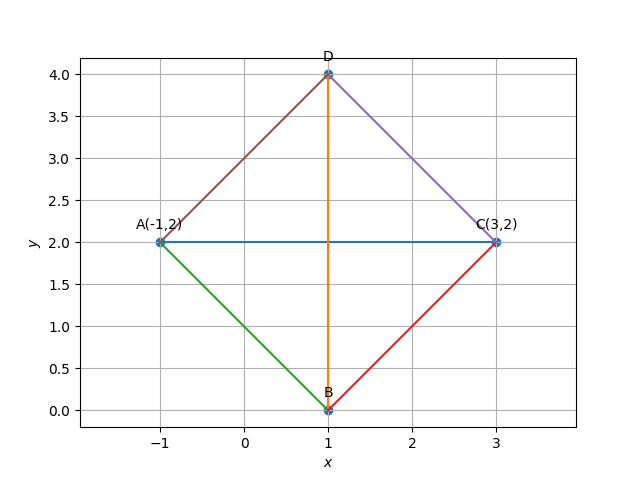
\includegraphics[width=\columnwidth]{chapters/10/7/4/4/figs/square}
	\end{center}
\caption{}
\label{fig:7/4/4/4Fig1}
\end{figure}

Shifting $\vec{A}$ to origin with reference to Fig. \ref{fig:7/4/4/4Fig2},
\begin{align}
\vec{A^{\prime}} =
\myvec{
0 \\
0\\
},
\vec{C^{\prime}} = \vec{C}-\vec{A} = 
\myvec{
4 \\
0\\
}
\end{align}

\begin{figure}[!h]
	\begin{center} 
	    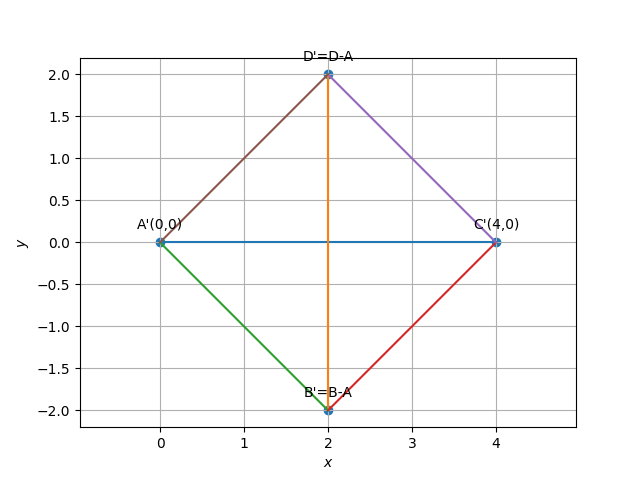
\includegraphics[width=\columnwidth]{chapters/10/7/4/4/figs/square1}
	\end{center}
\caption{}
\label{fig:7/4/4/4Fig2}
\end{figure}
\iffalse
In general,
the angle made by $AC$ with the x-axis is 
		\begin{align}
\beta = \theta + 45\degree
		\end{align}
\fi
Since
\begin{align}
\vec{C} - \vec{A} = \myvec{
4\\
0
} \equiv 
\myvec{
1\\
0
},
	\tan\theta&= \frac{0}{4} \implies 
\theta= 0\degree
\end{align}
		where
$\theta$ is the angle made by $AC$ with the x-axis.
Considering the rotation matrix 
\begin{align}
\vec{P} =
\myvec{
\cos\brak{\frac{\pi}{4}-\theta} & -\sin\brak{\frac{\pi}{4}-\theta} \\
\sin\brak{\frac{\pi}{4}-\theta} & \cos\brak{\frac{\pi}{4}-\theta} 
}
\end{align}
\iffalse
from Fig. \ref{fig:7/4/4/4Fig3},
\begin{align}
\vec{C^{\prime \prime}} = \vec{P}^\top (\vec{C}-\vec{A}) =
\myvec{
\frac{1}{\sqrt{2}} & -\frac{1}{\sqrt{2}} \\
\frac{1}{\sqrt{2}} & \frac{1}{\sqrt{2}}\\
}
\myvec{
4 \\
0\\
} = 
\myvec{
\frac{4}{\sqrt{2}} \\
\frac{4}{\sqrt{2}}\\
}
\end{align}
\begin{align}
\vec{B^{\prime \prime}} = \myvec{
 1&0\\
 0&0\\
}\vec{C^{\prime \prime}}=
\myvec{
 \frac{4}{\sqrt{2}}\\
 0\\
},
\vec{D^{\prime \prime}} = \myvec{
 0&0\\
 0&1\\
}\vec{C^{\prime \prime}}=
\myvec{
 0\\
 \frac{4}{\sqrt{2}}\\
} \text{ and }
\vec{A^{\prime \prime}} =
\myvec{
0 \\
0\\
}
\end{align}
\fi
\begin{figure}[!h]
	\begin{center} 
	    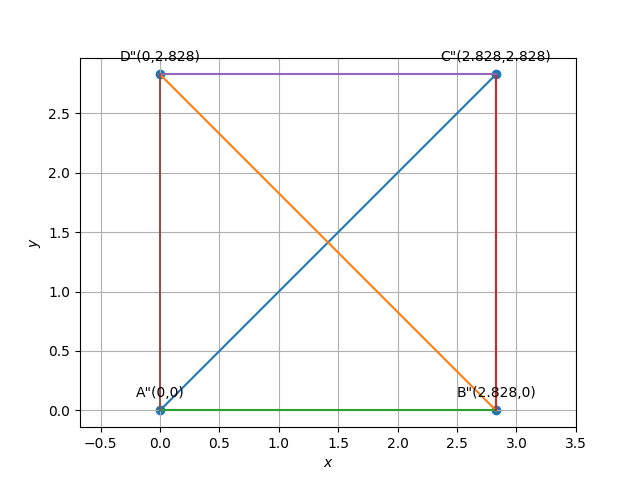
\includegraphics[width=\columnwidth]{chapters/10/7/4/4/figs/square2}
	\end{center}
\caption{}
\label{fig:7/4/4/4Fig3}
\end{figure}

\newpage
\iffalse
Again tranforming(rotating) the coordinates back to the original axis.

We know for anti-clockwise direction the rotation matrix is given as
\begin{align}
\vec{P} =
\myvec{
\cos\theta & -\sin\theta \\
\sin\theta & \cos\theta \\
}
\end{align}

Again we know that the angle is negative so the rotation will be in clockwise direction. So now the transformed(rotated) coordinates $\vec{B} \text{ and } \vec{D}$ are with refrence to 
\fi
from Figure 
%\ref{fig:7/4/4/4Fig4},
\ref{fig:7/4/4/4Fig3},
\begin{align}
	\vec{C^{\prime \prime}} &= \vec{P} (\vec{C}-\vec{A}) 
	\\
\label{eq:7/4/4/4bp}
	\vec{B^{\prime \prime}} &= \myvec{\vec{e}_1 & \vec{0}}\vec{C^{\prime \prime}}
	\\
\label{eq:7/4/4/4dp}
	\vec{D^{\prime \prime}} &= \myvec{ \vec{0} & \vec{e}_2}\vec{C^{\prime \prime}}
\end{align}
Now, 
\begin{align}
\label{eq:7/4/4/4b}
	\vec{B} = \vec{P}^{\top}\vec{B}^{\prime \prime}+\vec{A}
	\\
\label{eq:7/4/4/4d}
	\vec{D} = \vec{P}^{\top}\vec{D}^{\prime \prime}+\vec{A}
\end{align}
by reversing the process of translation and rotation.  Thus, 
from
\eqref{eq:7/4/4/4b}
\eqref{eq:7/4/4/4bp},
\eqref{eq:7/4/4/4d}
and
\eqref{eq:7/4/4/4dp}
\begin{align}
	\vec{B} = \vec{P}^{\top}\myvec{\vec{e}_1 & \vec{0}}\vec{P} (\vec{C}-\vec{A}) +\vec{A}
	\\
	\vec{D} = \vec{P}^{\top}\myvec{\vec{0} & \vec{e}_2  }\vec{P} (\vec{C}-\vec{A}) +\vec{A}
%	\vec{B} &= \brak{(\vec{C}-\vec{A})^{\top}\vec{P}^{\top} \vec{e}_1}\vec{P}^{\top}\vec{e}_1+\vec{A}
%	\\
%	\vec{D} &= \brak{(\vec{C}-\vec{A})^{\top}\vec{P}^{\top} \vec{e}_2}\vec{P}^{\top}\vec{e}_2+\vec{A}
\end{align}
yielding
		\begin{align}
\vec{B}=
\myvec{
1\\
0
},
\vec{D}
\myvec{
1\\
4
}.
		\end{align}
\iffalse
\begin{align}
\vec{B^{\prime}} &= \vec{P}\vec{B^{\prime \prime}} = \myvec{
\frac{1}{\sqrt{2}} & \frac{1}{\sqrt{2}} \\
-\frac{1}{\sqrt{2}} & \frac{1}{\sqrt{2}}\\
}
\myvec{
 \frac{4}{\sqrt{2}}\\
 0\\
} = 
\myvec{
2 \\
-2\\
}\\
\vec{D^{\prime}} &= \vec{P}\vec{D^{\prime \prime}} = \myvec{
\frac{1}{\sqrt{2}} & \frac{1}{\sqrt{2}} \\
-\frac{1}{\sqrt{2}} & \frac{1}{\sqrt{2}}\\
}
\myvec{
 0\\
 \frac{4}{\sqrt{2}}\\
} = 
\myvec{
2 \\
2 \\
}
\end{align}

\begin{figure}[!h]
	\begin{center} 
	    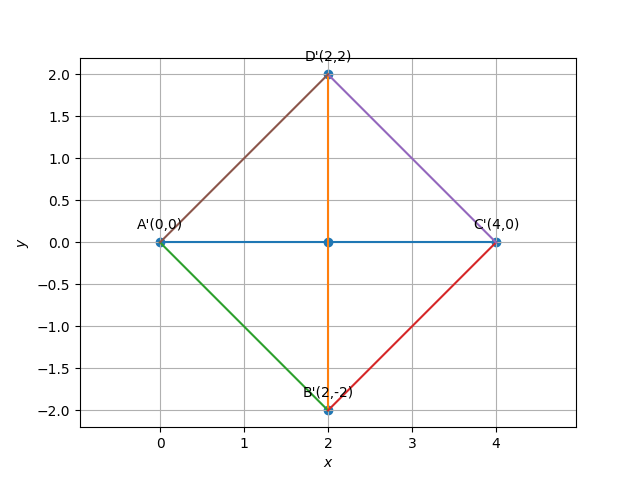
\includegraphics[width=\columnwidth]{chapters/10/7/4/4/figs/square3}
	\end{center}
\caption{}
\label{fig:7/4/4/4Fig4}
\end{figure}

Again transforming(shifting) the axis back to the original with refrence to Figure \ref{fig:7/4/4/4Fig5}
\begin{align}
\vec{B} &= \vec{B^{\prime}}+\vec{A} = \myvec{
2 \\
-2\\
}+\myvec{
-1 \\
2\\
} = 
\myvec{
1 \\
0\\
}\\
\vec{D} &= \vec{D^{\prime}}+\vec{A} = \myvec{
2 \\
2\\
}+\myvec{
-1 \\
2\\
} = 
\myvec{
1 \\
4 \\
}
\end{align}

Hence, the other two vertices are $\vec{B}(1,0) \text{ and } \vec{D}(1,4)$   

\begin{figure}[!h]
	\begin{center} 
	    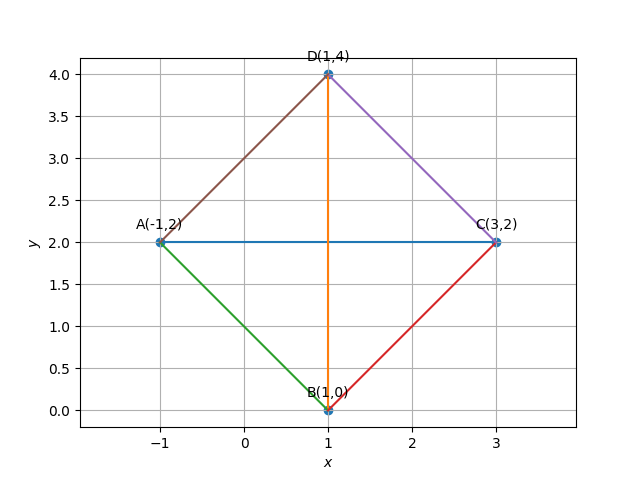
\includegraphics[width=\columnwidth]{chapters/10/7/4/4/figs/square4}
	\end{center}
\caption{}
\label{fig:7/4/4/4Fig5}
\end{figure}
which can also be expressed as
\begin{align}
\vec{B} &= \vec{A} + \vec{P}\myvec{
\vec{e_{1}}&\vec{0}\\
}
\vec{P}^\top \brak{\vec{C}-\vec{A}}\\
\vec{D} &= \vec{A} + \vec{P}\myvec{
\vec{0}&\vec{e_{2}}\\
}
\vec{P}^\top \brak{\vec{C}-\vec{A}}\\
\end{align}
where $\vec{P}$ is the rotation matrix and $\vec{A} \text{ and } \vec{C}$ are the position vectors of opposite vertices.

Derivation of the above formulas:

We know that after shifting the axis and rotating by the required angle any arbitrary square will be aligned with the x and y axis so that we can directly get the vectors $\vec{B} \text{ and } \vec{D}$ as follows
\begin{align}
\vec{C^{\prime\prime}} &= \vec{P}^\top \brak{\vec{C} - \vec{A}}\\
\vec{B^{\prime\prime}} &= \myvec{
\vec{e_{1}} & \vec{0}
}\vec{C^{\prime\prime}} = \myvec{
\vec{e_{1}} & \vec{0}
}\vec{P}^\top \brak{\vec{C} - \vec{A}}\\
\vec{B^{\prime}} &= \vec{P} \vec{B^{\prime\prime}}  = \vec{P}\myvec{
\vec{e_{1}} & \vec{0}
}\vec{P}^\top \brak{\vec{C} - \vec{A}}\\
\vec{B} &= \vec{A}+\vec{B^{\prime}}\\
 &= \vec{A} + \vec{P}\myvec{
\vec{e_{1}}&\vec{0}\\
}
\vec{P}^\top\brak{\vec{C}-\vec{A}}
\end{align}

Similarly for D it can be derived as
\begin{align}
\vec{C^{\prime\prime}} &= \vec{P}^\top \brak{\vec{C} - \vec{A}}\\
\vec{D^{\prime\prime}} &= \myvec{
\vec{0} & \vec{e_{2}}
}\vec{C^{\prime\prime}} = \myvec{
\vec{0} & \vec{e_{2}}
}\vec{P}^\top \brak{\vec{C} - \vec{A}}\\
\vec{D^{\prime}} &= \vec{P} \vec{D^{\prime\prime}} = \vec{P} \myvec{
\vec{0} & \vec{e_{2}}
}\vec{P}^\top \brak{\vec{C} - \vec{A}}\\
\vec{D} &= \vec{A}+\vec{D^{\prime}}\\
 &= \vec{A} + \vec{P}\myvec{
\vec{0}&\vec{e_{2}}\\
}
\vec{P}^\top\brak{\vec{C}-\vec{A}}
\end{align}


Verification of the above formula for the given question

\begin{align}
\vec{B} &= \myvec{
-1\\
2\\
}+\myvec{
\frac{1}{\sqrt{2}} & \frac{1}{\sqrt{2}} \\
-\frac{1}{\sqrt{2}} & \frac{1}{\sqrt{2}}\\
}\myvec{
 1&0\\
 0&0\\
}\myvec{
\frac{1}{\sqrt{2}} & -\frac{1}{\sqrt{2}} \\
\frac{1}{\sqrt{2}} & \frac{1}{\sqrt{2}}\\
}\myvec{
4\\
0\\
}\\
 &= \myvec{
-1\\
2\\
}+\myvec{
\frac{1}{\sqrt{2}} & \frac{1}{\sqrt{2}} \\
-\frac{1}{\sqrt{2}} & \frac{1}{\sqrt{2}}\\
}\myvec{
 1&0\\
 0&0\\
}\myvec{
\frac{4}{\sqrt{2}}\\
\frac{4}{\sqrt{2}}\\
}\\
 &= \myvec{
-1\\
2\\
}+\myvec{
\frac{1}{\sqrt{2}} & \frac{1}{\sqrt{2}} \\
-\frac{1}{\sqrt{2}} & \frac{1}{\sqrt{2}}\\
}\myvec{
\frac{4}{\sqrt{2}}\\
0\\
}\\
 &= \myvec{
-1\\
2\\
}+\myvec{
2\\
-2\\
}\\
 &= \myvec{
1\\
0\\
}\\
\vec{D} &= \myvec{
-1\\
2\\
}+\myvec{
\frac{1}{\sqrt{2}} & \frac{1}{\sqrt{2}} \\
-\frac{1}{\sqrt{2}} & \frac{1}{\sqrt{2}}\\
}\myvec{
 0&0\\
 0&1\\
}\myvec{
\frac{1}{\sqrt{2}} & -\frac{1}{\sqrt{2}} \\
\frac{1}{\sqrt{2}} & \frac{1}{\sqrt{2}}\\
}\myvec{
4\\
0\\
}\\
 &= \myvec{
-1\\
2\\
}+\myvec{
\frac{1}{\sqrt{2}} & \frac{1}{\sqrt{2}} \\
-\frac{1}{\sqrt{2}} & \frac{1}{\sqrt{2}}\\
}\myvec{
 0&0\\
 0&1\\
}\myvec{
\frac{4}{\sqrt{2}}\\
\frac{4}{\sqrt{2}}\\
}\\
 &= \myvec{
-1\\
2\\
}+\myvec{
\frac{1}{\sqrt{2}} & \frac{1}{\sqrt{2}} \\
-\frac{1}{\sqrt{2}} & \frac{1}{\sqrt{2}}\\
}\myvec{
0\\
\frac{4}{\sqrt{2}}\\
}\\
 &= \myvec{
-1\\
2\\
}+\myvec{
2\\
2\\
}\\
 &= \myvec{
1\\
4\\
}
\end{align}
\fi








\iffalse
\item The Class X students of a secondary school in Krishinagar have been allotted a rectangular plot of land for their gardening activity. Sapling of Gulmohar are planted on the boundary at a distance of 1m from each other. There is a triangular grassy lawn in the plot as shown in fig.\ref{fig:Fig1}. The students are to sow seeds of flowering plants on the remaining area of the plot.\\

\begin{figure}[!h]
	\begin{center} 
	    \includegraphics[width=\columnwidth]{./ss}
	\end{center}
\caption{}
\label{fig:Fig1}
\end{figure}
\item Taking $\vec{A}$ as origin, find the coordinates of the vertices of the triangle.
\item What will be the coordinates of the vertices of $\triangle PQR$ if $\vec{C}$ is the origin?
Also calculate the areas of the triangles in these cases. What do you observe?
\end{enumerate}

\fi

\item The vertices of a $\triangle ABC$ are $\vec{A}(4,6), \vec{B}(1,5)$ and  $\vec{C}(7,2)$. A line is drawn to intersect sides $AB$ and $AC$ at $\vec{D}$ and $\vec{E}$ respectively, such that $\frac{AD}{AB} = \frac{AE}{AC} = \frac{1}{4}$. Calculate the area of $\triangle ADE$ and compare it with the area of the $\triangle ABC$.

\item Let $\vec{A}(4, 2), \vec{B}(6, 5)$  and $ \vec{C}(1, 4)$ be the vertices of $\triangle ABC$.

\begin{enumerate}
\item The median from $\vec{A}$ meets $BC$ at $\vec{D}$. Find the coordinates of the point $\vec{D}$.
\item Find the coordinates of the point $\vec{P}$ on $AD$ such that $AP : PD = 2 : 1$.
\item Find the coordinates of points $\vec{Q}$ and $\vec{R}$ on medians $BE$ and $CF$ respectively such that $BQ : QE = 2 : 1$  and  $CR : RF = 2 : 1$.
\item What do you observe?
\item If $\vec{A}, \vec{B}$ and $\vec{C}$  are the vertices of $\triangle ABC$, find the coordinates of the centroid of the triangle.
\end{enumerate}
\solution
	\iffalse
\documentclass[12pt]{article}
\usepackage{graphicx}
\usepackage[none]{hyphenat}
\usepackage{graphicx}
\usepackage{listings}
\usepackage[english]{babel}
\usepackage{graphicx}
\usepackage{caption} 
\usepackage{booktabs}
\usepackage{array}
\usepackage{amssymb} % for \because
\usepackage{amsmath}   % for having text in math mode
\usepackage{extarrows} % for Row operations arrows
\usepackage{listings}
\usepackage[utf8]{inputenc}
\lstset{
  frame=single,
  breaklines=true
}
\usepackage{hyperref}
  
%Following 2 lines were added to remove the blank page at the beginning
\usepackage{atbegshi}% http://ctan.org/pkg/atbegshi
\AtBeginDocument{\AtBeginShipoutNext{\AtBeginShipoutDiscard}}


%New macro definitions
\newcommand{\mydet}[1]{\ensuremath{\begin{vmatrix}#1\end{vmatrix}}}
\providecommand{\brak}[1]{\ensuremath{\left(#1\right)}}
\newcommand{\solution}{\noindent \textbf{Solution: }}
\newcommand{\myvec}[1]{\ensuremath{\begin{pmatrix}#1\end{pmatrix}}}
\providecommand{\norm}[1]{\left\lVert#1\right\rVert}
\providecommand{\abs}[1]{\left\vert#1\right\vert}
\let\vec\mathbf

\begin{document}

\begin{center}
\title{\textbf{VECTORS}}
\date{\vspace{-5ex}} %Not to print date automatically
\maketitle
\end{center}

\section{10$^{th}$ Maths - EXERCISE-7.4}

Let A(4, 2), B(6, 5) and C(1, 4) be the vertices of $\triangle ABC$
\begin{enumerate}
\item The median from A meets BC at D. Find the coordinates of the point D.
\item Find the coordinates of the point P on AD such that $AP : PD = 2 : 1$
\item Find the coordinates of points Q and R on medians BE and CF respectively such
that $BQ : QE = 2 : 1 \text{and} CR : RF = 2 : 1.$
\item What do yo observe?
\item If $A(x_1, y_1), B(x_2, y_2) \text{and} C(x_3, y_3)$ are the vertices of $\triangle ABC$, find the coordinates of the centroid of the triangle.
\end{enumerate}

Given points are
\begin{align}
\vec{A}=\myvec{4\\ 2} ,
\vec{B}=\myvec{6\\ 5} ,
\vec{C}=\myvec{1\\ 4}
\end{align}
\fi

\begin{enumerate}
\item 
\begin{align}
\vec{D}&=\frac{\vec{B}+\vec{C}}{2}\\
&=\myvec{\frac{7}{2}\\[2pt] \frac{9}{2}}\\
\vec{E}&=\frac{\vec{A}+\vec{C}}{2}\\
&=\myvec{\frac{5}{2}\\ 3}\\
\vec{F}&=\frac{\vec{A}+\vec{B}}{2}\\
&=\myvec{5\\ \frac{7}{2}}
\end{align}

\item 
	For
$n=2$,
\begin{align}
\vec{P}&=\frac{1}{1+n}\brak{\myvec{\vec{A}+n\vec{D}}}\\
&=\frac{1}{3}\myvec{11\\11}
\end{align}

\item 
\begin{align}
\vec{Q}&=\frac{1}{1+n}\brak{\myvec{\vec{B}+n\vec{E}}}\\
&=\frac{1}{3}\myvec{11\\11}\\
\vec{R}&=\frac{1}{1+n}\brak{\myvec{\vec{C}+n\vec{F}}}\\
&=\frac{1}{3}\myvec{11\\11}\\
\end{align}

\item 
 $\vec{P},\vec{Q},\vec{R}$ are the same point.
   
\item 
\begin{align}
\vec{G}&=\frac{\vec{D}+\vec{E}+\vec{F}}{3}\\
&=\frac{1}{3}\myvec{11\\11}\\
\end{align} 
\end{enumerate}
See Fig.  
  \ref{fig:chapters/10/7/4/7/Figure}.
\begin{figure}[h!]
\centering
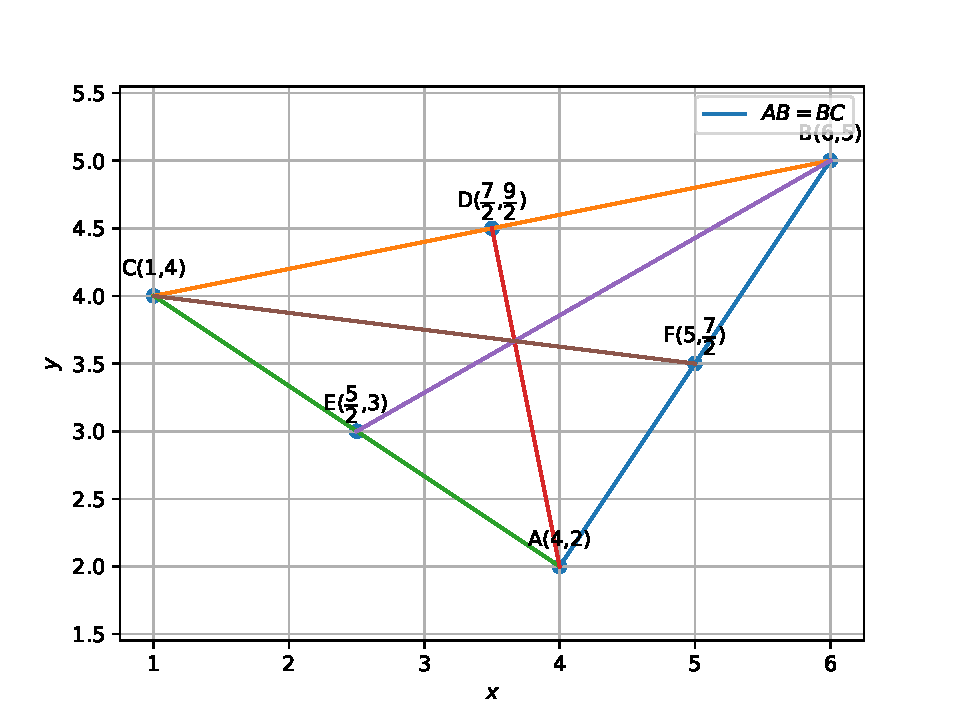
\includegraphics[width=\columnwidth]{chapters/10/7/4/7/figs/dj.pdf}
\caption{}
  \label{fig:chapters/10/7/4/7/Figure}
\end{figure}



\item $ABCD$ is a rectangle formed by the points $\vec{A}(–1, –1), \vec{B}(– 1, 4), \vec{C}(5, 4)$  and  $\vec{D}(5, – 1)$. $\vec{P}, \vec{Q}, \vec{R}$ and $\vec{S}$ are the mid-points of $AB, BC, CD$ and $DA$ respectively. Is the quadrilateral $PQRS$ a square? a rectangle? or a rhombus? Justify your answer.
	\\
	\iffalse
\documentclass[12pt]{article}
\usepackage{graphicx}
%\documentclass[journal,12pt,twocolumn]{IEEEtran}
\usepackage[none]{hyphenat}
\usepackage{graphicx}
\usepackage{listings}
\usepackage[english]{babel}
\usepackage{graphicx}
\usepackage{caption} 
\usepackage{hyperref}
\usepackage{booktabs}
\usepackage{array}
\usepackage{amsmath}   % for having text in math mode
\usepackage{listings}
\lstset{
  frame=single,
  breaklines=true
}
  
%Following 2 lines were added to remove the blank page at the beginning
\usepackage{atbegshi}% http://ctan.org/pkg/atbegshi
\AtBeginDocument{\AtBeginShipoutNext{\AtBeginShipoutDiscard}}
%


%New macro definitions
\newcommand{\mydet}[1]{\ensuremath{\begin{vmatrix}#1\end{vmatrix}}}
\providecommand{\brak}[1]{\ensuremath{\left(#1\right)}}
\providecommand{\norm}[1]{\left\lVert#1\right\rVert}
\newcommand{\solution}{\noindent \textbf{Solution: }}
\newcommand{\myvec}[1]{\ensuremath{\begin{pmatrix}#1\end{pmatrix}}}
\let\vec\mathbf

\begin{document}

\begin{center}
\title{\textbf{Properties of Quadrilaterals}}
\date{\vspace{-5ex}} %Not to print date automatically
\maketitle
\end{center}

\setcounter{page}{1}



\section{10$^{th}$ Maths - Chapter 7}

This is Problem-8 from Exercise 7.4

\begin{enumerate}
\item ABCD is a rectangle formed by the points $\vec{A}(–1, –1), \vec{B}(– 1, 4), \vec{ C}(5, 4) \text{ and } \vec{D}(5, – 1)$. $\vec{P,Q,R} \text{ and } \vec{S}$ are the mid-points of $\vec{AB, BC, CD} \text{ and } \vec{DA}$ respectively. Is the quadrilateral
PQRS a square? a rectangle? or a rhombus? Justify your answer. \\
\fi
\solution 
See Fig. \ref{fig:10/7/4/8Fig3}.
\begin{align}
  \label{eq:10/7/4/8det2f}
  \vec{P} &= \frac{1}{2}\brak{\vec{A}+\vec{B}} =   \frac{1}{2}\brak{\myvec{
  -1 \\
  -1 \\
 } + \myvec{
  -1 \\
  4 \\
 } 
 } = \myvec{
 -1 \\
 \frac{3}{2} \\
 }   \\
 \vec{Q} &= \frac{1}{2}\brak{\vec{B}+\vec{C}} =   \frac{1}{2}\brak{\myvec{
  -1 \\
  4 \\
 } + \myvec{
  5 \\
  4 \\
 } 
 } = \myvec{
 2 \\
 4 \\
 }   \\
 \vec{R} &= \frac{1}{2}\brak{\vec{C}+\vec{D}} =   \frac{1}{2}\brak{\myvec{
  5 \\
  4 \\
 } + \myvec{
  5 \\
  -1\\
 } 
 } = \myvec{
 5 \\
 \frac{3}{2} \\
 }   \\
 \vec{S} &= \frac{1}{2}\brak{\vec{D}+\vec{A}} =   \frac{1}{2}\brak{\myvec{
  5 \\
  -1 \\
 } + \myvec{
  -1 \\
  -1\\
 } 
 } = \myvec{
 2\\
 -1 \\
 }   
\end{align}

\begin{figure}[!h]
	\begin{center}
		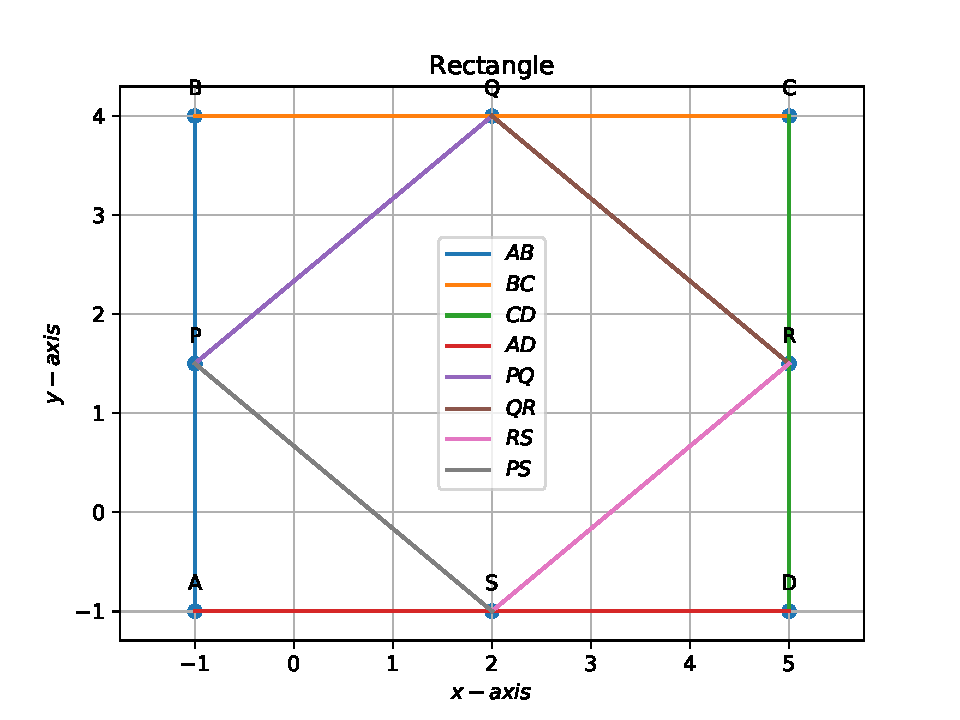
\includegraphics[width=\columnwidth]{chapters/10/7/4/8/figs/problem1.pdf}
	\end{center}
\caption{}
\label{fig:10/7/4/8Fig3}
\end{figure}
We know that PQRS is a parallelogram. To know, if it is a rectangle, we need to ascertain whether any of the two adjacent sides are perpendicular. 
That means $\brak{\vec{Q}-\vec{P}}^\top\brak{\vec{R}-\vec{Q}}$ should be equal to zero. 
\begin{align}
\vec{Q}-\vec{P} &=  \myvec{
 2 \\
 4 \\
 } - \myvec{
 -1 \\
 \frac{3}{2} \\
 } = \myvec{
 3 \\
 \frac{5}{2} \\ 
 } \\
 \vec{R}-\vec{Q} &=  \myvec{
 5 \\
 \frac{3}{2}\\
 } - \myvec{
 2 \\
 4 \\
 } = \myvec{
 3 \\
 -\frac{5}{2} \\ 
 } \\ 
 \brak{\vec{Q}-\vec{P}}^\top\brak{\vec{R}-\vec{Q}} &= \myvec{
 3 & \frac{5}{2}} \myvec{
 3 \\
 -\frac{5}{2} 
 } \neq 0
\end{align}
Therefore PQRS is not a rectangle. Let us check if it is a rhombus. For a rhombus, the diagonals bisect perpendicularly. That means $\brak{\vec{R}-\vec{P}}^\top\brak{\vec{S}-\vec{Q}}$ should be equal to zero. 
\begin{align}
\vec{R}-\vec{P} &=  \myvec{
 5 \\
 \frac{3}{2} \\
 } - \myvec{
 -1 \\
 \frac{3}{2} \\
 } = \myvec{
 6 \\
 0 \\ 
 } \\
 \vec{S}-\vec{Q} &=  \myvec{
 2 \\
 -1 \\
 } - \myvec{
 2 \\
 4 \\
 } = \myvec{
 0 \\
 -5 \\ 
 } \\ 
 \brak{\vec{R}-\vec{P}}^\top\brak{\vec{S}-\vec{Q}} &= \myvec{
 6 & 0} \myvec{
 0 \\
 -5 \\
 } = 0
\end{align}
Therefore $PQRS$ is a rhombus.




\end{enumerate}




\section{Line Preliminaries}
\begin{enumerate}

\item 
\label{chapters/11/10/1/1}
\iffalse
\documentclass[journal,12pt,twocolumn]{IEEEtran}
\usepackage[none]{hyphenat}
\usepackage{graphicx}
\usepackage{listings}
\usepackage[english]{babel}
\usepackage{graphicx}
\usepackage{caption} 
\usepackage{amsmath}
\usepackage{hyperref}
\usepackage{booktabs}
\usepackage{array}
\let\vec\mathbf
\title{\textbf{\\Line Assignment}}
\author{Sinkona Chinthamalla - FWC22054}
\begin{document}
\maketitle

\section{Question}
\textbf{\textit{Class 11, Exercise 10.1, Q(1):}
\fi
Draw a quadrilateral in the Cartesian plane, whose vertices are 
(-4,5), (0,7), (5,-5), (-4,-2). Also, find its area.
\\
\solution See Fig. 
		\ref{fig:11/10/1/1}.
	\begin{figure}[!ht]
		\centering
 \includegraphics[width=\columnwidth]{chapters/11/10/1/1/figs/quadrilateral.png}
		\caption{}
		\label{fig:11/10/1/1}
  	\end{figure}
\iffalse
}

\begin{figure}[h!]
\centering
\includegraphics[scale=0.35]{quadrilateral.png}
\centering
\caption{Quadrilateral ABCD}
\end{figure}

\section{Construction}
\centering
\vspace{0.2cm}
{
\setlength\extrarowheight{2pt}
\begin{tabular}{|c|c|c|}
	\hline
	\textbf{Symbol}&\textbf{Value}&\textbf{Description}\\
	\hline
	A & $\begin{pmatrix}
     -4 \\
      5 
    \end{pmatrix}$ & Vertex A\\
	\hline
	B & $\begin{pmatrix}
     0 \\
     7 
    \end{pmatrix}$ & Vertex B\\
	\hline
	C & $\begin{pmatrix}
      5 \\
     -5 
    \end{pmatrix}$ & Vertex C\\
	\hline
	D & $\begin{pmatrix}
     -4 \\
     -2 
    \end{pmatrix}$ & Vertex D\\
	\hline
\end{tabular}
}

\section{Solution}
\raggedright 
We can divide the quadrilateral into two triangles, one with sides \textbf{AB}, \textbf{BC}, and \textbf{AC}, and the other with sides \textbf{AC}, \textbf{CD}, and \textbf{AD}.\\
\vspace{0.2cm}
\textbf{1. Finding area using Matrices} \\
\vspace{0.25cm}
Consider $ \triangle ABC, $
\vspace{0.2cm}
\begin{equation}
ar(\triangle \vec{ABC})= \frac{1}{2} \myvec{
                    \vec{x_1} & \vec{y_1} & 1\\
                    \vec{x_2} & \vec{y_2} & 1\\
                    \vec{x_3} & \vec{y_3} & 1
                   } 
\end{equation} 
\begin{center}
$ = \frac{1}{2} \myvec{
                    -4 & 5 & 1\\
                     0 & 7 & 1\\
                     5 & -5 & 1
                   } $ \\
                   \vspace{0.2cm}
\end{center}
\vspace{0.2cm}
\raggedright
\begin{equation}
ar(\triangle ABC)= 29 \quad sq.units 
\end{equation}  
\\( Since area cannot be negative )

\begin{figure}[h]
\centering
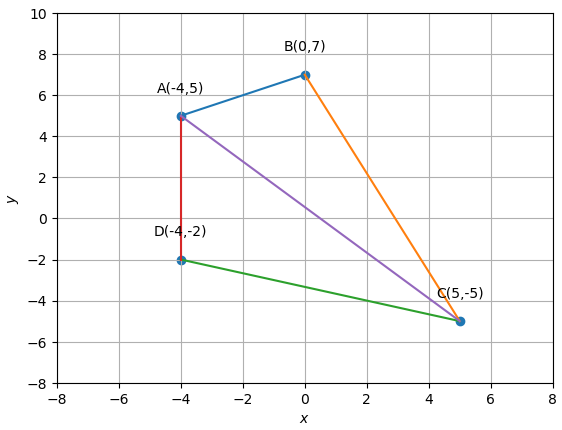
\includegraphics[scale=0.35]{diagnol.png}
\centering
\caption{Quadrilateral ABCD with diagonal AC}
\end{figure}

\vspace{0.3cm}
\noindent Now consider $ \triangle ADC, $
\begin{equation}
ar(\triangle \vec{ADC})= \frac{1}{2} \myvec{
                    \vec{x_1} & \vec{y_1} & 1\\
                    \vec{x_2} & \vec{y_2} & 1\\
                    \vec{x_3} & \vec{y_3} & 1
                   } 
\end{equation} 
\begin{center}
$ = \frac{1}{2} \myvec{
                    -4 &  5 & 1\\
                    -4 & -2 & 1\\
                     5 & -5 & 1
                   } $
\end{center}
\vspace{0.2cm}
\begin{equation}
ar(\triangle ADC)= 31.5 \quad sq.units 
\end{equation}

\boldmath
\vspace{0.2cm}
\textbf{Area of Quadrilateral ABCD} 
\begin{equation}
 = ar(\triangle ABC)+ar(\triangle ADC)
\end{equation}
\begin{center}
 = 60.5  sq.units
\end{center}

\newpage
\vspace{0.2cm} 
\textbf{2. Finding area using Cross product} \\
\vspace{0.25cm}
\fi
\begin{align}
	ar(\triangle ABC)&= \frac{1}{2}\norm{\brak{\vec{B}-\vec{A}} \times \brak{\vec{B}-\vec{C}}} 
	\\
	&= \frac{1}{2} \mydet{
                    4 & 2\\
                   -5 & 12
	   }
= 29 
\end{align}
Similarly,
\begin{align}
	ar(\triangle ADC)&= \frac{1}{2}\norm{\brak{\vec{D}-\vec{A}} \times \brak{\vec{D}-\vec{C}}}
	\\
	&= \frac{1}{2} \mydet{
                    0 & -7\\
                   -9 &  3
                   } 
= 31.5
\end{align}
Thus, 
\begin{align}
	ar(ABCD)
	&= ar(\triangle ABC)+ar(\triangle ADC) 
	= 60.5 
\end{align}

\iffalse
\vspace{1cm}
Get the python code from
\begin{table}[h]
\large
\centering
\begin{tabular}{|l|}
\hline
https://github.com/SinkonaChinthamalla/fwc/
\\blob/main/matrix/line/codes \\
\hline
\end{tabular}
\end{table}	
\end{document}
\fi

\item 
\label{chapters/11/10/1/2}
\iffalse
\documentclass[journal,12pt,twocolumn]{IEEEtran}
\usepackage{graphicx}
\usepackage{listings}
\usepackage[utf8]{inputenc}
\usepackage{caption}
\usepackage{hyperref}
\usepackage[cmex10]{amsmath}
\usepackage{array}
\usepackage{gensymb}
\usepackage{booktabs}
\usepackage{etoolbox}
\patchcmd{\section}{\centering}{}{}{}
\providecommand{\norm}[1]{\left\lVert#1\right\rVert}
\providecommand{\abs}[1]{\left\vert#1\right\vert}
\let\vec\mathbf
\newcommand{\myvec}[1]{\ensuremath{\begin{pmatrix}#1\end{pmatrix}}}
\newcommand{\mydet}[1]{\ensuremath{\begin{vmatrix}#1\end{vmatrix}}}
\providecommand{\brak}[1]{\ensuremath{\left(#1\right)}}
\makeatletter
\newcommand\xleftrightarrow[2][]{%
  \ext@arrow 9999{\longleftrightarrowfill@}{#1}{#2}}
\newcommand\longleftrightarrowfill@{%
  \arrowfill@\leftarrow\relbar\rightarrow}
\makeatother
\title{Matrix Problems \textbf{\\Straight Lines }}
\author{Manoj Chavva} 

\begin{document}
\maketitle



\section{Problem Statement}

\noindent 
\fi
The base of an equilateral triangle with side $2a$ lies along the y-axis such that the mid-point of the base is at the origin. Find vertices of the triangle.
	\begin{figure}[!ht]
		\centering
 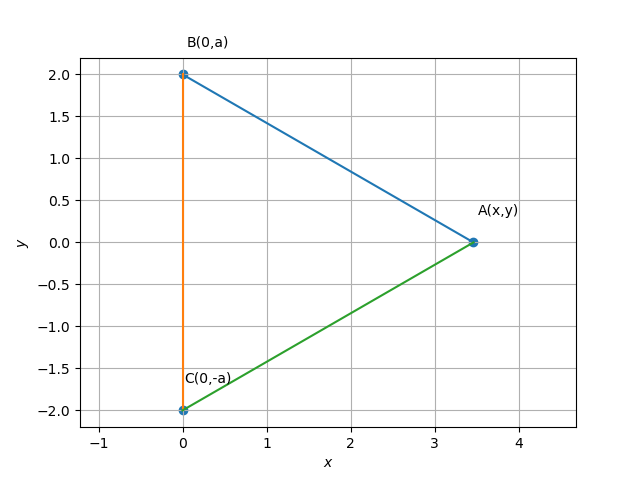
\includegraphics[width=\columnwidth]{chapters/11/10/1/2/figs/triangle.png}
		\caption{}
		\label{fig:11/10/1/2}
  	\end{figure}
	\\
	\solution Let the base be $BC$.  From the given information, 
\begin{align}
	\vec{B} = a\vec{e}_2,
	\vec{C} = -a\vec{e}_2
\end{align}
Since $\vec{A}$ lies on the $x$-axis, 
\begin{align}
	\vec{A} = k\vec{e}_1
\end{align}
and 
\begin{align}
	\norm{\vec{A}-\vec{C}}^2 &= \brak{2a}^2
	\\
	\implies \norm{\vec{A}}^2+\norm{\vec{C}}^2 - 2 \vec{A}^{\top}\vec{C} &= 4a^2
	\\
	\implies k^2 +a^2 &= 4a^2
	\\
	\text{or, } k = \pm a\sqrt{3}
\end{align}
Thus, 
\begin{align}
	\vec{A} = \pm \sqrt{3}a\vec{e}_1
\end{align}
		Fig. \ref{fig:11/10/1/2}
		is plotted for $a = 2$.

\iffalse

\begin{figure}[h]
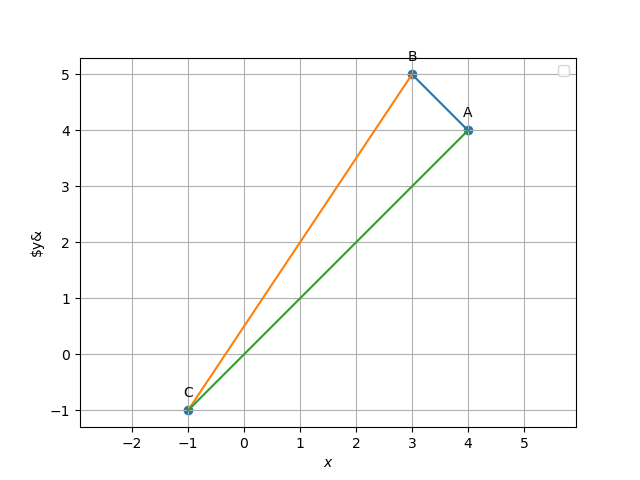
\includegraphics[width=1\columnwidth]{triangle.png}
\caption{Equilateral Triangle ABC}
\label{fig:triangle}
\end{figure}

\section{Construction}
B and C are the inputs.
\begin{table}[h]
\centering
\large
\begin{tabular}{|l|l|l|}
\hline
\textbf{Symbol} & \textbf{Value} & \textbf{Description} \\ \hline
B               & \myvec{0 \\ 2}         & Vertex B             \\ \hline
C               & \myvec{0 \\ -2}        & Vertex C             \\ \hline
A               & \myvec{x \\ y}          & Vertex A             \\ \hline
A1              & \myvec{x1 \\ y1}       & Vertex A             \\ \hline
\end{tabular}
\end{table}

\section{Solution}
\noindent Given the base with 2a is lies on the y-axis with the mid-point of the base is at origin. The vertices of the two points on y-axis will be

\begin{equation}
\vec{B}=\begin{pmatrix} 
0\\
a
\end{pmatrix}, {
\vec{C}=\begin{pmatrix} 
0\\
-a
\end{pmatrix} }
\end{equation}
\noindent Given $\Delta$ABC is an equilateral triangle i.e 
\begin{equation}
 \norm{\vec{A}-\vec{B}}= \norm{\vec{B}-\vec{C}}= \norm{\vec{C}-\vec{A}} =2a
\end{equation}

%\noindent As AB = AC, triangle is isoceles and by properties of isoceles triangle, altitude is perpendicular bisector of base.\\
%
%\noindent Therefore $\angle$AOC = $\angle$AOB = $90^0$ and $\norm{\vec{O}-\vec{B}}= \norm{\vec{O}-\vec{C}}= a$ \\
%
%\noindent By Cosine laws,
%\begin{equation}
%\cos\vec{B} = \cos\vec{C} = a* \frac{1}{2a} = \frac{1}{2}
%\end{equation}
%\begin{equation}
%\angle B = \angle C = \arccos\frac{1}{2} = 60^0
%\end{equation}
% \begin{equation}
% \angle A = 180^0 -(60^0 * 2) = 60^0
%  \end{equation}
%\noindent Therefore, the equilaterial triangle have all internal angles eaqual to  $60^0$ 

\noindent Consider, two sides of equilateral triangle be $\vec{A}$ and $\vec{B}$ then the third side will be $ \vec{A} -\vec{B}$ 
%Hence,
%\begin{equation}
%\norm{\vec{a}-\vec{b}}^2 = l
%\end{equation}
%\begin{equation}
%\brak{\vec{a}-\vec{b}}^{\top} \brak{\vec{a}-\vec{b}} = l^2
%\end{equation}
%\begin{equation}
%l^2 = 2 \vec{a}^{\top} \cdot \vec{b}
%\end{equation}
%\begin{equation}
%l^2 = 2 \norm{\vec{a}}\norm{\vec{b}} \cos\theta
%\end{equation}
%\begin{equation}
%\theta = \arccos\frac{1}{2} = 60^0
\begin{equation}
\norm{\vec{A}}=\norm{\vec{B}}=\norm{\vec{A-B}}\\
\end{equation}
\begin{equation}
\norm{\vec{A}}^2=\norm{\vec{B}}^2=\norm{\vec{A-B}}^2\\
\end{equation}
\begin{equation}
\norm{\vec{A}}^2+\norm{\vec{B}}^2-2\vec{A}^T\vec{B}=\norm{\vec{A}}^2=\norm{\vec{B}}^2\\
\end{equation}
\begin{equation}
\frac{\vec{A}^T\vec{B}}{\norm{\vec{A}}^2}=\frac{\vec{A}^T\vec{B}}{\norm{\vec{B}^2}}=\frac{1}{2}
\end{equation}
%$\triangle$OAB is a equilateral triangle\\

\noindent Therefore, the  triangle have all internal angles eaqual to  $60^0$

The angle between two vectors is given by 
  \begin{align}
    \label{eq:angle2d}
    \theta = \cos^{-1}\frac{\vec{A}^{\top} \vec{B}}{\norm{A}\norm{B}}
  \end{align}

 \begin{equation}  
  \brak{\vec{x}-\vec{B}}^{\top} \brak{\vec{x}-\vec{C}}= \norm{\vec{x}-\vec{B}} \cdot \norm{\vec{x}-\vec{C}} \cdot \cos\theta 
 \end{equation}

 \begin{equation}  
\brak{\vec{x}^\top \cdot \vec{x}} - \brak{\vec{x}^\top \cdot \vec{C}} - \brak{\vec{B}^\top \cdot \vec{x}} - \brak{\vec{B}^\top \cdot \vec{C}} = 2a \cdot 2a \cos 60^0   
 \end{equation}

 \begin{equation}  
\norm{\vec{x}}^2 - \vec{x}^\top\brak{\vec{B}+\vec{C}} - \vec{B}^\top \cdot \vec{C} = 2a \cdot 2a \cdot \frac{1}{2}
 \end{equation}

  \begin{equation}  
\norm{\vec{x}}^2 - \vec{x}^\top\brak{0} -\myvec{0 \\ a} \myvec{0 & -a}  = 4a^2
 \end{equation}

\begin{equation}
\norm{\vec{x}}^2 + a^2 = 4a^2
\end{equation}

\begin{equation}
\norm{\vec{x}}^2 = 3a^2
\label{eq-1}
\end{equation}
Considering, the line equation of $\vec{AB}$

\begin{equation}
\norm{\vec{x}-\vec{B}}^2 = 4a^2
\end{equation}

\begin{equation}
\brak{\vec{x} -\vec{B}}^{\top} \cdot \brak{\vec{x}-\vec{B}} = 4a^2
\end{equation}

\begin{equation}
\norm{\vec{x}}^2-2\cdot \vec{x}^\top \vec{B} + \norm{\vec{B}}^2 = 4a^2
\end{equation}

\begin{equation}
3a^2 - 2\cdot \vec{x}^\top \vec{B} + a^2 = 4a^2
\end{equation}

\begin{equation}
\vec{x}^\top \vec{B} = 0
\end{equation}
\noindent Since we can write, \begin{equation}
\vec{B} = a \cdot \vec{e}_2
\end{equation}

\begin{equation}
\vec{x}^\top \cdot a \cdot \vec{e}_2 = 0
\end{equation}

\begin{equation}
\vec{x}^\top \cdot \vec{e}_2 = 0
\end{equation}

\begin{equation}
\vec{x} = \lambda \vec{e}_1
\end{equation}

\noindent From this its clearly concluded that third vertex will lie on x-axis. 
\noindent From the equation \eqref{eq-1} 
\begin{equation}
\vec{x} = \sqrt{3}{a}
\end{equation}


\noindent Hence,the coordinates of the vertices of triangle are 
  \begin{equation*}
\vec{A} = 
   \begin{pmatrix}
   \pm\sqrt{3}a \\ 0
 \end{pmatrix}
 \end{equation*}

\begin{equation}
\vec{B}=\begin{pmatrix} 
0\\
a
\end{pmatrix}, {
\vec{C}=\begin{pmatrix} 
0\\
-a
\end{pmatrix} }
\end{equation}



\begin{table}[h]
\large
\begin{tabular}{lll}
\multicolumn{3}{l}{Get Python Code for image from}                                                 \\ \hline
\multicolumn{3}{|l|}{\url{https://github.com/ManojChavva/FWC/blob/main/Matrix/line/code-py/triangle.py}} \\ 
 \hline
\multicolumn{3}{l}{Get LaTex code from}                                                            \\ \hline
\multicolumn{3}{|l|}{\url{https://github.com/ManojChavva/FWC/blob/main/Matrix/line/line.tex}}            \\ \hline
\end{tabular}
\end{table}

\end{document}

\fi

\item 
\label{chapters/11/10/1/4}
\iffalse
\documentclass[journal,10pt,twocolumn]{article}
\usepackage{graphicx}
\usepackage[margin=0.5in]{geometry}
\usepackage[cmex10]{amsmath}
\usepackage{array}
\usepackage{booktabs}
\usepackage{makecell}
\title{\textbf{Line Assignment}}
\author{Hari Venkateswarlu}
\date{September 2022}
\usepackage[framemethod=tikz]{mdframed}
\newcommand{\myvec}[1]{\ensuremath{\myvec{#1}}}
\let\vec\mathbf
\newcommand{\mydet}[1]{\ensuremath{\begin{vmatrix}#1\end{vmatrix}}}
\providecommand{\mbf}{\mathbf}
\providecommand{\pr}[1]{\ensuremath{\Pr\left(#1\right)}}
\providecommand{\qfunc}[1]{\ensuremath{Q\left(#1\right)}}
\providecommand{\sbrak}[1]{\ensuremath{{}\left[#1\right]}}
\providecommand{\lsbrak}[1]{\ensuremath{{}\left[#1\right.}}
\providecommand{\rsbrak}[1]{\ensuremath{{}\left.#1\right]}}
\providecommand{\brak}[1]{\ensuremath{\left(#1\right)}}
\providecommand{\lbrak}[1]{\ensuremath{\left(#1\right.}}
\providecommand{\rbrak}[1]{\ensuremath{\left.#1\right)}}
\providecommand{\cbrak}[1]{\ensuremath{\left\{#1\right\}}}
\providecommand{\lcbrak}[1]{\ensuremath{\left\{#1\right.}}
\providecommand{\rcbrak}[1]{\ensuremath{\left.#1\right\}}}

\begin{document}

\maketitle
\paragraph{\textit{Problem Statement} - 
\fi
	\begin{figure}[!ht]
		\centering
 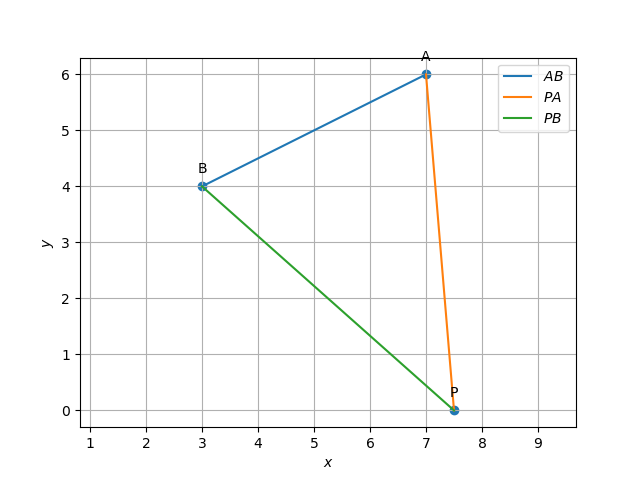
\includegraphics[width=\columnwidth]{chapters/11/10/1/4/figs/line.png}
		\caption{}
		\label{fig:11/10/1/4}
  	\end{figure}
	\\
	\solution 
\iffalse
 }
\begin{center}
    \label{tab:truthtable}
    \setlength{\arrayrulewidth}{0.2mm}
\setlength{\tabcolsep}{5pt}
\renewcommand{\arraystretch}{1.25}
    \begin{tabular}{|c|c|c|}
    \hline % <-- Alignments: 1st column left, 2nd middle and 3rd right, with vertical lines in between
      \large\textbf{Symbol} & \large\textbf{Co-ordinates} & \large\textbf{Description}\\
      \hline
       \large A & $\ \myvec{ 7\\ 6 }$ & co-ordinates of A \\
       \large B & $\ \myvec{ 3\\ 4 }$ & co-ordinates of B \\
	
	
      \hline
   \end{tabular}
 \end{center}\vspace{5mm}

\begin{figure}[h]
\centering
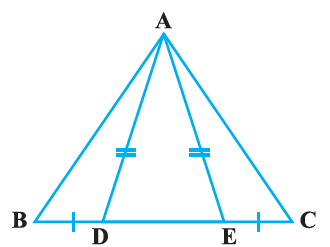
\includegraphics[width=1\columnwidth]{Figure1.png}

\label{fig}
\end{figure}

\section*{Solution}
1. Given points
A=$\myvec{
  7 \\
  6 \\
 }$
 and B=$\myvec{
  3 \\
  4 \\
 }$


\raggedright 2. If the point is lying on x-axis then y-axis will be zero i.e.. y=0

\fi
From the given information

\begin{align}
	\norm{\vec{x}-\vec{A}}^2 &=\norm{\vec{x}-\vec{B}}^2
	\\
	\implies
	\brak{\vec{x}-\vec{A}}^{\top} \brak{\vec{x}-\vec{A}} &= \brak{\vec{x}-\vec{B}}^{\top} \brak{\vec{x}-\vec{B}}
	\\
	\implies     \norm{\vec{x}}^2 - 2\vec{A}^{\top}\vec{x} + \norm{\vec{A}}^2 &= \norm{\vec{x}}^2 - 2\vec{B}^{\top}\vec{x} + \norm{\vec{B}}^2
	\\
	\text{or, }
	\brak{\vec{A}-\vec{B}}^{\top}   \vec{x}&= \frac{\norm{\vec{A}}^2 - \norm{\vec{B}}^2}{2}
		\label{eq:11/10/1/4}
\end{align}  
Since $\vec{x}$ lies on the $x$-axis,
\begin{align}
	\vec{x} &=k\vec{e}_1
\end{align}  
which, upon substituting in 
		\eqref{eq:11/10/1/4}
		yields
\begin{align}
	k = \frac{15}{2}
\end{align}
\iffalse
$\vec{(A-B)^{\top}x} = \frac{\|\vec{A}\|^2 - \|\vec{B}\|^2}{2}$\\ \vspace{2mm}
     $\myvec{0 & 1 \\ 4 & 2}x = $\myvec{0 \\ 30}\\ \vspace{2mm}
      $\myvec{0 & 1 & 0 \\ 4 & 2 & 30}$\\    \vspace{2mm}
      Divide by 2\\
      $\myvec{0 & 1 & 0 \\ 2 & 1 & 15}$\\    \vspace{2mm}
     $\myvec{2 & 1 & 15 \\ 0 & 1 & 0}
    \xleftarrow[]{R_2 \leftarrow R_1}$\\     \vspace{2mm}
    $\myvec{1 & \frac{1}{2} & \frac{15}{2} \\ 0 & 1 & 0}\xleftarrow[]{{R_1}=\frac{R_1}{2}}$\\            \vspace{2mm}
    $\myvec{1 & 0 & \frac{15}{2} \\ 0 & 1 & 0}\xleftarrow[]{{R_1}={R_1}-\frac{R_2}{2}}$\\             \vspace{2mm}
    $\myvec{1 & 0 & 7.5 \\ 0 & 1 & 0}$\\        \vspace{2mm}
on solving we get x = 7.5\\
\vspace{2mm}
  x=$\myvec{
  7.5 \\
  0 \\
 }$               			
\end{document}
\fi

\item 
%\label{chapters/11/10/1/4}
%\iffalse
\documentclass[journal,10pt,twocolumn]{article}
\usepackage{graphicx}
\usepackage[margin=0.5in]{geometry}
\usepackage[cmex10]{amsmath}
\usepackage{array}
\usepackage{booktabs}
\usepackage{makecell}
\title{\textbf{Line Assignment}}
\author{Hari Venkateswarlu}
\date{September 2022}
\usepackage[framemethod=tikz]{mdframed}
\newcommand{\myvec}[1]{\ensuremath{\myvec{#1}}}
\let\vec\mathbf
\newcommand{\mydet}[1]{\ensuremath{\begin{vmatrix}#1\end{vmatrix}}}
\providecommand{\mbf}{\mathbf}
\providecommand{\pr}[1]{\ensuremath{\Pr\left(#1\right)}}
\providecommand{\qfunc}[1]{\ensuremath{Q\left(#1\right)}}
\providecommand{\sbrak}[1]{\ensuremath{{}\left[#1\right]}}
\providecommand{\lsbrak}[1]{\ensuremath{{}\left[#1\right.}}
\providecommand{\rsbrak}[1]{\ensuremath{{}\left.#1\right]}}
\providecommand{\brak}[1]{\ensuremath{\left(#1\right)}}
\providecommand{\lbrak}[1]{\ensuremath{\left(#1\right.}}
\providecommand{\rbrak}[1]{\ensuremath{\left.#1\right)}}
\providecommand{\cbrak}[1]{\ensuremath{\left\{#1\right\}}}
\providecommand{\lcbrak}[1]{\ensuremath{\left\{#1\right.}}
\providecommand{\rcbrak}[1]{\ensuremath{\left.#1\right\}}}

\begin{document}

\maketitle
\paragraph{\textit{Problem Statement} - 
\fi
	\begin{figure}[!ht]
		\centering
 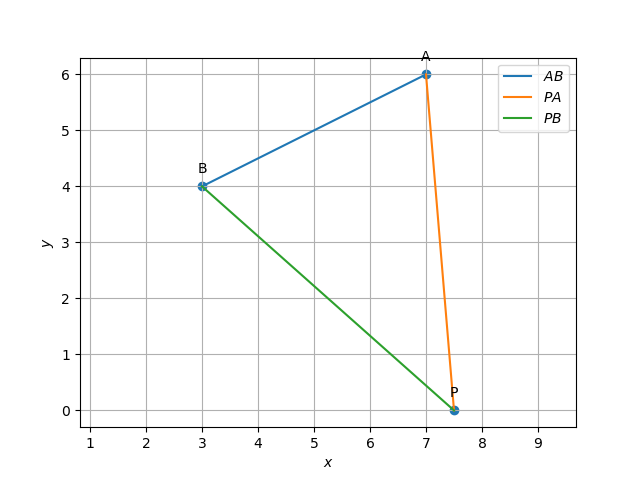
\includegraphics[width=\columnwidth]{chapters/11/10/1/4/figs/line.png}
		\caption{}
		\label{fig:11/10/1/4}
  	\end{figure}
	\\
	\solution 
\iffalse
 }
\begin{center}
    \label{tab:truthtable}
    \setlength{\arrayrulewidth}{0.2mm}
\setlength{\tabcolsep}{5pt}
\renewcommand{\arraystretch}{1.25}
    \begin{tabular}{|c|c|c|}
    \hline % <-- Alignments: 1st column left, 2nd middle and 3rd right, with vertical lines in between
      \large\textbf{Symbol} & \large\textbf{Co-ordinates} & \large\textbf{Description}\\
      \hline
       \large A & $\ \myvec{ 7\\ 6 }$ & co-ordinates of A \\
       \large B & $\ \myvec{ 3\\ 4 }$ & co-ordinates of B \\
	
	
      \hline
   \end{tabular}
 \end{center}\vspace{5mm}

\begin{figure}[h]
\centering
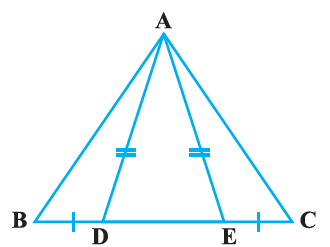
\includegraphics[width=1\columnwidth]{Figure1.png}

\label{fig}
\end{figure}

\section*{Solution}
1. Given points
A=$\myvec{
  7 \\
  6 \\
 }$
 and B=$\myvec{
  3 \\
  4 \\
 }$


\raggedright 2. If the point is lying on x-axis then y-axis will be zero i.e.. y=0

\fi
From the given information

\begin{align}
	\norm{\vec{x}-\vec{A}}^2 &=\norm{\vec{x}-\vec{B}}^2
	\\
	\implies
	\brak{\vec{x}-\vec{A}}^{\top} \brak{\vec{x}-\vec{A}} &= \brak{\vec{x}-\vec{B}}^{\top} \brak{\vec{x}-\vec{B}}
	\\
	\implies     \norm{\vec{x}}^2 - 2\vec{A}^{\top}\vec{x} + \norm{\vec{A}}^2 &= \norm{\vec{x}}^2 - 2\vec{B}^{\top}\vec{x} + \norm{\vec{B}}^2
	\\
	\text{or, }
	\brak{\vec{A}-\vec{B}}^{\top}   \vec{x}&= \frac{\norm{\vec{A}}^2 - \norm{\vec{B}}^2}{2}
		\label{eq:11/10/1/4}
\end{align}  
Since $\vec{x}$ lies on the $x$-axis,
\begin{align}
	\vec{x} &=k\vec{e}_1
\end{align}  
which, upon substituting in 
		\eqref{eq:11/10/1/4}
		yields
\begin{align}
	k = \frac{15}{2}
\end{align}
\iffalse
$\vec{(A-B)^{\top}x} = \frac{\|\vec{A}\|^2 - \|\vec{B}\|^2}{2}$\\ \vspace{2mm}
     $\myvec{0 & 1 \\ 4 & 2}x = $\myvec{0 \\ 30}\\ \vspace{2mm}
      $\myvec{0 & 1 & 0 \\ 4 & 2 & 30}$\\    \vspace{2mm}
      Divide by 2\\
      $\myvec{0 & 1 & 0 \\ 2 & 1 & 15}$\\    \vspace{2mm}
     $\myvec{2 & 1 & 15 \\ 0 & 1 & 0}
    \xleftarrow[]{R_2 \leftarrow R_1}$\\     \vspace{2mm}
    $\myvec{1 & \frac{1}{2} & \frac{15}{2} \\ 0 & 1 & 0}\xleftarrow[]{{R_1}=\frac{R_1}{2}}$\\            \vspace{2mm}
    $\myvec{1 & 0 & \frac{15}{2} \\ 0 & 1 & 0}\xleftarrow[]{{R_1}={R_1}-\frac{R_2}{2}}$\\             \vspace{2mm}
    $\myvec{1 & 0 & 7.5 \\ 0 & 1 & 0}$\\        \vspace{2mm}
on solving we get x = 7.5\\
\vspace{2mm}
  x=$\myvec{
  7.5 \\
  0 \\
 }$               			
\end{document}
\fi

\item 
\label{chapters/11/10/1/5}
\iffalse
\documentclass[journal,12pt,twocolumn]{IEEEtran}
\usepackage{graphicx}
\graphicspath{{./figs/}}{}
\usepackage{amsmath,amssymb,amsfonts,amsthm}
\newcommand{\myvec}[1]{\ensuremath{\begin{pmatrix}#1\end{pmatrix}}}

\let\vec\mathbf

\title{
Matrix-Lines
}
\author{Jyothsna Paluchuri-FWC22059\\}
\begin{document}
\maketitle
\tableofcontents
\bigskip
\section{Problem Statement}
\fi
	\begin{figure}[!ht]
		\centering
 \includegraphics[width=\columnwidth]{chapters/11/10/1/5/figs/line.png}
		\caption{}
		\label{fig:11/10/1/5}
  	\end{figure}
	\\
	\solution
\iffalse
\section{Construction}
\begin{figure}[h]
    \centering
\includegraphics[width=\columnwidth]{line.png}
    \caption{Equation of the slope}
    \label{fig:my_label}
\end{figure}
\vspace{2cm}
\begin{table}[h]
    \centering
    \begin{tabular}{|c|c|c|c|}
       \hline
       \textbf{Symbol}&\textbf{Value}&\textbf{Description}  \\
       \hline
	    $\vec{P}$ & $\myvec{
		    0\\
		    -4}$
	    & Point on Y-axis\\
        \hline
	    $\vec{B}$ & $\myvec{8\\0}$
 & Point on X-axis\\
        \hline
	    $\vec{0}$ & $\myvec{0\\0}$
 & Origin\\
        \hline
    \end{tabular}
    \caption{Parameters}
    \label{tab:my_label}
\end{table}


\section{Solution}
Given that resultant line passes through origin and mid point of the line segment joining point P(0,-4) and B(8,0) \\
\\
\\
given ${\vec{P}}$=$\myvec{
  0\\
  -4}$
 , ${\vec{B}}$=$\myvec{
  8\\
  0}$
  
 \fi 
The mid point of $PB$ is
\begin{align}
\vec{M} &=\frac{1}{2}(\vec{P}+\vec{B})
	= \myvec{4 \\ -2}  
\end{align}
The direction vector of line joining $\vec{O}, \vec{M}$ is 
\begin{align}
\vec{m}&=\vec{O}-\vec{M}
 = -\vec{M}
\end{align}
which can be expressed as
\begin{align}
	\myvec{1 \\ -\frac{1}{2}}
\end{align}
Thus the slope is
\begin{align}
	m = -\frac{1}{2}
\end{align}
\iffalse
\textbf{The direction vector of a line expressed as}
\begin{align}
\implies\vec{m} &= \begin{pmatrix}1 \\ m \\ \end{pmatrix}
\end{align}

\textbf{By solving equation (5) and (6),we get the slope of $\vec{O}$ $\vec{M}$ line}
\begin{align}
        \boxed{m=-0.5}
 \end{align}

\section{Software}
Download the following code using,
\begin{table}[h]
    \centering
    \begin{tabular}{|c|}
    \hline \\
   https://github.com/jyothsna777/jyothsna-fwc.git  \\
         \\
\hline
    \end{tabular}
\end{table}
\\
and execute the code by using command
\begin{center}
\textbf{Python3 lines.py}\\
\end{center}

\section{Conclusion}
Hence the slope of line $\vec{O}$ $\vec{M}$ lineis $\vec{m}$=-0.5

\end{document}
\fi

\item 
\label{chapters/11/10/1/6}
\iffalse
\documentclass[journal,12pt,twocolumn]{IEEEtran}
\usepackage[none]{hyphenat}
\usepackage{graphicx}
\usepackage{listings}
\usepackage[english]{babel}
\usepackage{graphicx}
\usepackage{caption} 
\usepackage{amsmath}
\usepackage{hyperref}
\usepackage{booktabs}
\usepackage{array}


\title{\textbf{\\Assignment on line}}
\author{Sireesha Abbavaram - FWC22060}
\begin{document}
\maketitle


\section{Question}
\textbf{\textit{Class 11, Exercise 10.1, Q(6):}
\fi
	\begin{figure}[!ht]
		\centering
 \includegraphics[width=\columnwidth]{chapters/11/10/1/6/figs/triangle.png}
		\caption{}
		\label{fig:11/10/1/6}
  	\end{figure}
\iffalse
}

\begin{figure}[h!]
\centering
\includegraphics[scale=0.35]{triangle.png}
\centering
\caption{Traingle ABC}
\end{figure}


\section{Solution}
\raggedright 
\vspace{0.25cm}
Let A,B and C be the vertices of a given traingle with coordinates $\myvec{
4 \\
4
}
, \myvec{
3 \\
5
}
 and \myvec{
-1 \\
-1
} $
\raggedright
. we have verify whther the given vertices are of right angled triangle or not.\\
\begin{center}
\raggedright
Let The directional vector of two vectors A and B is given as AB (m1)=A-B.
\end{center}
\vspace{0.25cm}
\begin{center}
The directional vector of the vectors B and C is given as BC (m2)=B-C.
\end{center}
\vspace{0.25cm}
\begin{center}
The directinal vector of the vectors C and A is given as CA (m3)=C-A.
\end{center}
\vspace{0.25cm}
The angle between any two vectors is given by
\boldmath
\\ $ cos b =\frac{(m1)^T(m2)}{||m1|| ||m2||}  equation-1$
\unboldmath
\vspace{0.5cm}\raggedright\\
Where b is the angle between the two vectors .
when the angle b=90 ,we get cos 90=0.
\vspace{0.5cm}\raggedright\\
It implies that the numerator of the equation 1 should be zero.

\vspace{0.25cm}
 In order to prove that the triangle is right angled we have to show any two vectors should be orthogonal to each other.
 
\vspace{0.25cm}\raggedright
So we need to show $(A-B)^T(B-C) or (B-C)^T(C-A) or (C-A)^T(A-B) $ is equal to zero.
\fi

\vspace{0.5cm}\raggedright
\begin{align}
	\vec{C}-\vec{A}&=\myvec{
-5 \\
	-5},
\\
	\vec{A}-\vec{B}&=\myvec{
1 \\
-1 
}
\\
	\implies \brak{\vec{C}-\vec{A}}^{\top}
	\brak{\vec{A}-\vec{B}}&=0
\end{align}
Thus, $AB \perp AC$.
\iffalse
\vspace{0.25cm}\raggedright
Thus we have right angle at the vertex A.


\vspace{0.2cm}
\section*{Construction}
\centering
\vspace{0.2cm}
{
\setlength\extrarowheight{2pt}
\begin{tabular}{|c|c|c|}
	\hline
	\textbf{Symbol}&\textbf{Value}&\textbf{Description}\\
	\hline
	A & (4,4) & Vertex A\\
	\hline
	B & (3,5) & Vertex B\\
	\hline
	C & (-1,-1) & Vertex C\\
	\hline
	
\end{tabular}
}

\vspace{0.6cm}
Get the python code of the figures from
\begin{table}[h]
\large
\centering
\begin{tabular}{|l|}
\hline
https://github.com/Sireesha1602/sireesha/
\\blob/main/line assignment \\
\hline
\end{tabular}

\end{table}




\end{document}
\fi

\item 
\label{chapters/11/10/1/8}
\iffalse
\documentclass[10pt, a4paper]{article}
\usepackage[a4paper,outer=1.5cm,inner=1.5cm,top=1.75cm,bottom=1.5cm]{geometry}

\twocolumn
\usepackage{graphicx}

\usepackage{hyperref}
\usepackage[utf8]{inputenc}
\usepackage{amsmath}
\usepackage{physics}
\usepackage{amssymb}
\begin{document}
\title{Assignment-4}
\author{Name:C.CHANDANA\and Email :  \url{cheenepallichandana531@gmail.com}}
%\{ Wireless Communication (FWC)}
\date{30-sep-2022}
\maketitle



\section{Problem}
\fi
If three points $(x, -1), (2, 1)$ and $(4, 5)$ are collinear, find the value of $x$.
\\
\solution 
	\begin{figure}[!ht]
		\centering
 \includegraphics[width=\columnwidth]{chapters/11/10/1/8/figs/sline.png}
		\caption{}
		\label{fig:11/10/1/8}
  	\end{figure}
	\iffalse
\begin{center}
	\fi
	Let
\begin{align} \label{eq:11/10/1/8}
	\vec{A}=\myvec{ x\\ -1 },
	\vec{B}=\myvec{ 2\\ 1 },
\vec{C}=\myvec{ 4\\ 5 }.
\end{align}
Then
\begin{align}
\vec{A}-\vec{B}
	&=\myvec{ x-2\\ -2 }
	\\
\vec{A}-\vec{C}
	&=\myvec{ 4-x\\ 6 }
\end{align}
Forming the collinearity matrix
using 
	\eqref{eq:normal_line-collinear},
\begin{align} 
\myvec{ x-2 & -2\\ 4-x & 6  } 
	\xleftrightarrow[]{{R_1=3R_1+R-2}}
=\myvec{
2x-2 &0 \\ 
 4-x& 6
}
\end{align}

\iffalse

In the problem they have given that three points lie on a line, thats means these three points are collinear.\\

If  points on a line  are  collinear, rank of matrix is " 1 "then the vectors are in linearlydependent.\\
For 2 × 2 matrix Rank =1 means Determinant is 0.\\

Through pivoting,we obtain\\
\begin{align}
=\myvec{ x-2 & -2\\ 4-x & 6 \ } \\ 
\end{align}
\begin{align}
=\myvec{
x-2 &-2 \\ 
 4-x& 6
}\overset{R1=3R1+R2}{\rightarrow}
=\myvec{
2x-2 &0 \\ 
 4-x& 6
}
\end{align} 
\fi
	If the rank of the matrix is 1, any one of the rows must be zero. So, making the first element in the above matrix 0,
\begin{align}
x=1
\end{align} 

\iffalse

\begin{align}\label{eq:11/10/1/8}
x=1 \\
\end{align} 

Hence proved.\\
\section{Construction}
 \begin{figure}[h]
\centering
\includegraphics[scale=0.4]{sline.png} 
\caption{}
\end{figure}
\section{Code}
*Verify the above proofs in the following code.\\
\framebox{
\url{https://github.com/chandana531/FWC/tree/main/matrix/line}}	
\bibliographystyle{ieeetr}
\end{document}
\fi

\item 
\label{chapters/11/10/1/9}
\iffalse
\documentclass[journal,12pt,twocolumn]{IEEEtran}
\usepackage[none]{hyphenat}
\usepackage{graphicx}
\usepackage{listings}
\usepackage[english]{babel}
\usepackage{graphicx}
\usepackage{caption} 
\usepackage{amsmath}
\usepackage{hyperref}
\usepackage{booktabs}
\usepackage{array}
\usepackage{stix}


\title{\textbf{\\Line Assignment}}
\author{kanekal kousar}
\date{September 2022}

\providecommand{\norm}[1]{\left\lVert#1\right\rVert}
\providecommand{\abs}[1]{\left\vert#1\right\vert}
\let\vec\mathbf
\newcommand{\myvec}[1]{\ensuremath{\myvec{#1}}}
\newcommand{\mydet}[1]{\ensuremath{\begin{vmatrix}#1\end{vmatrix}}}
\providecommand{\brak}[1]{\ensuremath{\left(#1\right)}}

\begin{document}
\maketitle


\section{Question}
\textbf{\textit{Class 11, Exercise 10.1, Q(9):} 
\fi
Without using distance formula, show that points (– 2, – 1), (4, 0), (3, 3) and (–3, 2) are the vertices of a parallelogram.
	\begin{figure}[!ht]
		\centering
 \includegraphics[width=\columnwidth]{chapters/11/10/1/9/figs/paralellogram.png}
		\caption{}
		\label{fig:11/10/1/9}
  	\end{figure}
	\\
	\solution See Fig. 
		\ref{fig:11/10/1/9}.
\iffalse
}

\section{Solution}
\raggedright 

\begin{figure}[h!]
\centering
\includegraphics[scale=0.5]{fig/paralellogram.png}  
\caption{paralellogram ABCD}
\end{figure}

\vspace{0.25cm}
We can prove that the points are the vertices of a parallelogram if the direction vectors of opposite lines are equal

Consider  figure I,where
\fi


\begin{align}
\vec{A}=\myvec{-2 \\ -1  },  \vec{B}=\myvec{ 4\\ 0 }, 
\vec{C}=\myvec{3 \\ 3  },  \vec{D}=\myvec{-3 \\ 2  }
\end{align}
and
\begin{align}
	\vec{P} &=\vec{B}-\vec{A}=\myvec{6 \\ 1 \\ }
	\\
	\vec{Q}&=\vec{C}-\vec{D}=\myvec{6 \\ 1 \\ }
	\\
	\vec{R}&=\vec{A}-\vec{C}=\myvec{1 \\ -3 \\ }
	\\
	\vec{S}&=\vec{A}-\vec{D}=\myvec{1 \\ -3 \\ }
\end{align}
Since
$\vec{P}=\vec{Q}$
and 
$\vec{R}=\vec{S}$, from  
	  \eqref{eq:two-pgm},
$ABCD$ is a 
parallelogram
\iffalse

\section*{Construction}
\centering
\vspace{0.2cm}
{
\setlength\extrarowheight{2pt}
\begin{tabular}{|c|c|c|}
	\hline
	\textbf{Symbol}&\textbf{Value}&\textbf{Description}\\
	\hline
	A & $\myvec{-2 \\ -1 \\ }$ & Vertex A\\
	\hline
	B & $\myvec{4 \\ 0 \\ }$ & Vertex B\\
	\hline
	C &$\myvec{3 \\ 3 \\ }$ & Vertex C\\
	\hline
	D & $\myvec{-3 \\ 2 \\ }$ & Vertex D\\
	\hline
	P &$\myvec{1 \\ 6 \\ }$&vector AB\\
	\hline
	Q&$\myvec{1 \\ 6 \\ }$&vector DC\\
	\hline
	R&$\myvec{1 \\ -3 \\ }$&vector BC\\
	\hline
	S&$\myvec{1 \\ -3 \\ }$&vector AD\\
	\hline
\end{tabular}
}

\vspace{0.6cm}
Get the python code of the figures from
\begin{table}[h]
\large
\centering
\framebox{
\url{https://github.com/kkousar/KOUSAR_FWC/blob/main/line_assignment/code/line.py}}
\bibliographystyle{ieeetr}

\end{table}



\end{document}
\fi

\item 
\label{chapters/11/10/1/10}
\iffalse
\def\mytitle{PYTHON PROGRAMMING ON MATRICES}
\def\myauthor{Revathi pamujula}
\def\contact{revathipamujula111@gmail.com}
\def\mymodule{Future Wireless Communication (FWC)}


\documentclass[10pt, a4paper]{article}
\usepackage[a4paper,outer=1.5cm,inner=1.5cm,top=1.75cm,bottom=1.5cm]{geometry}

\twocolumn
\usepackage{graphicx}
%\usepackage{karnaugh-map}
\usepackage{tabularx}
\usepackage{hyperref}
\usepackage[utf8]{inputenc}
\usepackage{amsmath}
%\usepackage{physics}
\usepackage{amssymb}
\usepackage{watermark}
\renewcommand*\familydefault{\sfdefault}
\usepackage{lipsum}
\usepackage{xcolor}
\usepackage{listings}
\let\vec\mathbf
\lstset{
frame=single, 
breaklines=true,
columns=fullflexible
}

\begin{document}
\title{\mytitle}
\author{\myauthor\hspace{1em}\\\contact\\FWC22045\hspace{6.5em}IITH\hspace{0.5em}\mymodule\hspace{6em}Matrix:Lines}

%\{ Wireless Communication (FWC)}
\date{}
\maketitle


  \section{Problem}
  \fi
\\
\solution See Fig. 
		\ref{fig:11/10/1/10}.
	\begin{figure}[!ht]
		\centering
 \includegraphics[width=\columnwidth]{chapters/11/10/1/10/figs/fig.png}
		\caption{}
		\label{fig:11/10/1/10}
  	\end{figure}

	\iffalse
\section{Solution}
\textbf{Given that:}
\begin{center}

%\boldmath
	\fi
	Let 
\begin{align}
\vec{P}=\myvec{ 3\\ -1 },
\vec{Q}=\myvec{ 4\\ -2 }
\end{align}
Then 
\begin{align}
	\vec{C}=\vec{P}-\vec{Q}
=\myvec{ -1\\ 1 }
\end{align}
The desired angle is given by
\begin{align}
	\cos\theta&=\frac{\vec{C}^{T}\vec{e}_1}{\norm{\vec{C}}\norm{\vec{e}_1}}
	\\
	&= -\frac{1}{\sqrt{2}}
	\\
	\implies 
	\theta&=135\degree
 \end{align}
 \iffalse
\begin{figure}[h!]
  \includegraphics[scale=0.5]{fig.png}
  \caption{line assignment }
  \label{fig:line assignment}
\end{figure}
\end{document}
\fi

\item 
\label{chapters/11/10/1/11}
\iffalse
\documentclass[10pt,a4paper]{report}
%\usepackage[latin1]{inputenc}
\usepackage[utf8]{inputenc}
\usepackage{amsmath}
\usepackage{amsfonts}
\usepackage{amssymb}
\usepackage{graphicx}
\usepackage{multicol}
\usepackage{tabularx}
\usepackage{tikz}
\usetikzlibrary{arrows,shapes,automata,petri,positioning,calc}
\usepackage{hyperref}
\usepackage{tikz}
\usetikzlibrary{matrix,calc}
\usepackage[margin=0.5in]{geometry}
% ---- power functions -----% 
\newcommand{\myvec}[1]{\ensuremath{\begin{pmatrix}#1\end{pmatrix}}}
\let\vec\mathbf

\providecommand{\norm}[1]{\left\lVert#1\right\rVert}
\providecommand{\abs}[1]{\left\vert#1\right\vert}
\let\vec\mathbf

\newcommand{\mydet}[1]{\ensuremath{\begin{vmatrix}#1\end{vmatrix}}}
\providecommand{\brak}[1]{\ensuremath{\left(#1\right)}}
\providecommand{\lbrak}[1]{\ensuremath{\left(#1\right.}}
\providecommand{\rbrak}[1]{\ensuremath{\left.#1\right)}}
\providecommand{\sbrak}[1]{\ensuremath{{}\left[#1\right]}}
%-------end power functions----%
\newenvironment{Figure}
  {\par\medskip\noindent\minipage{\linewidth}}
  {\endminipage\par\medskip}
\begin{document}
%--------------------logo figure-------------------------%
\begin{figure*}[!tbp]
  \centering
  \begin{minipage}[b]{0.4\textwidth}
    \includegraphics[scale = 0.05]{iitlogo.jpg}
  \end{minipage}
  \hfill
  \vspace{5mm}\begin{minipage}[b]{0.4\textwidth}
\raggedleft  \includegraphics[scale = 0.10]{nrc.png}\

  \end{minipage}\vspace{0.2cm}
\end{figure*}
%--------------------name & rollno-----------------------
\raggedright \textbf{Name}:\hspace{1mm} D. Siva Krishna\hspace{3cm} \Large \textbf{Assignment-4}\hspace{2.5cm} % 
\normalsize \textbf{Roll No.} :\hspace{1mm} FWC22065\vspace{1cm}
\begin{multicols}{2}

%----------------problem statement--------------%
\raggedright \textbf{Problem Statement:}\vspace{2mm}
\raggedright \\
\fi
	The slope of a line is double of the slope of another line. If tangent of the angle between them is 1/3, find the slopes of the lines.
	\begin{figure}[!ht]
		\centering
 \includegraphics[width=\columnwidth]{chapters/11/10/1/11/figs/line.png}
		\caption{}
		\label{fig:11/10/1/11}
  	\end{figure}
	\iffalse
\vspace{5mm}
%-----------------------------solution---------------------------
\raggedright \textbf{SOLUTION}:\vspace{2mm}\\

%---------given----------------%
\raggedright \textbf{Given}:\vspace{2mm}\\
Slope of one line is double of the slope of the other line. \\\vspace{1mm}
\fi
\\
\solution 
The direction vector of a line is expressed as
\begin{align}
\vec{m}=\myvec{1\\m}
\end{align}
where  $m$ is defined to be the slope of the line. If the angle between the lines be $\theta$,
\begin{align}
\tan \theta = \frac{1}{3}
\implies \cos \theta=\frac{3}{\sqrt{10}}
\end{align}
\iffalse
%--------------steps----------------------%
\textbf{Input Parameters:}
\vspace{2mm}


\begin{tabular}{|c|c|c|}
	\hline
	\textbf{Symbol}&\textbf{Value}&\textbf{Description}\\
	\hline
	$\vec{m_1}$ &\myvec{1\\m}& Direction vector\\
	\hline
    $\vec{m_2}$ &\myvec{1\\2m}&Direction vector\\
	\hline
    $\tan\theta$ &1/3& Angle\\
	\hline
\end{tabular}
\\
\vspace{10cm}
\fi
The angle between two vectors is then expressed as
\iffalse
\begin{align}
\cos \theta = \frac{^\top \textbf{B}}{\norm{\textbf{A}}\norm{\textbf{B}}}
\end{align} 
%Substituting the \vec{m_1} and \vec{m_2} in the above equation
\\
\fi
\begin{align}
	\frac{3}{\sqrt{10}} &= \frac{\vec{m}_1^\top \vec{m}_2}{\norm{\vec{m}_1}\norm{\vec{m}_2}}
	\\
	&= \frac{\myvec{1 &  m}\myvec{1 \\ 2m}}{\norm{\myvec{1\\m}}\norm{\myvec{1\\2m}}}
\\
	&= \frac{2m^2 +1}{\sqrt{m^2 + 1}\sqrt{4m^2 + 1}}
	\\
	\implies \frac{9}{10}&=\frac{4m^4 + 4m^2 +1}{4m^4 + 5m^2 +1}
\\
	\text{or, } 4m^4 - 5m^2 +1 = 0
\end{align}
\iffalse
Let $m^2$ = x and substituting it in above equation we get a quadratic equation.
\begin{align}
	4x^2 -5x +1 = 0
\end{align}
From the formula of fining roots of a quadratic equation
\begin{align}
	\frac{-b\pm \sqrt{b^2 - 4ac}}{2a}
	\\
	\\
	\frac{5\pm \sqrt{\left (-5\right )^2 - 16}}{8}
	\\
	x= 1 (or) x = 1/4
\end{align}
\\
The slope of the first line is
\\
\fi
yielding
\begin{align}
m=\pm \frac{1}{2}, 
\pm 1
\end{align}
\iffalse
$\therefore $ Slope of second line is
\begin{center}
$ 2m=\pm 1$\\
    (or)\\
    $2m=\pm 2$
\end{center}
\begin{center}
 \includegraphics[width=0.5\textwidth]{line.png}  
 \end{center}\vspace{1mm}
\raggedright  Download the code \\
Github link:{Assignment-4}.
\end{multicols}
\end{document}
\fi

\item 
\label{chapters/11/10/1/12}
\iffalse 
\documentclass[journal,12pt,twocolumn]{IEEEtran}
\usepackage{graphicx}
\graphicspath{{./figs/}}{}
\usepackage{amsmath,amssymb,amsfonts,amsthm}
\newcommand{\myvec}[1]{\ensuremath{\begin{pmatrix}#1\end{pmatrix}}}

\let\vec\mathbf

\title{
Matrix-Lines
}
\author{R.Radhika}
\begin{document}
\maketitle
\tableofcontents
\bigskip
\section{Problem Statement}
\fi
\\
\solution 
	\begin{figure}[!ht]
		\centering
 \includegraphics[width=\columnwidth]{chapters/11/10/1/12/figs/figure.pdf}
		\caption{}
		\label{fig:11/10/1/12}
  	\end{figure}
\iffalse
\section{Construction}
\begin{figure}[h]
    \centering
\includegraphics[width=\columnwidth]{figure.pdf}
    \caption{Equation of the slope}
    \label{fig:my_label}
\end{figure}
\vspace{2cm}
\begin{table}[h]
    \centering
    \begin{tabular}{|c|c|c|}
       \hline
       \textbf{Symbol}&\textbf{Value}&\textbf{Description}  \\
       \hline
	    $\vec{A}$ & $\myvec{
		    x_1\\
		    y_1}$
	    & Point on X-axis\\
        \hline
	    $\vec{B}$ & $\myvec{h\\k}$
 & Point on Y-axis\\
        \hline
        \hline
        A & k-y1=m(h-x1) & Given Condition\\
        \hline
    \end{tabular}
    \caption{Parameters}
    \label{tab:my_label}
\end{table}


\section{Solution}
Given that resultant line passes through point(x1,y1) and (h,k) (let prove the equation in vector form by line eqation ) \\
\\
\\
\fi
Given 
\begin{align}
\vec{A}=\myvec{
  x_1\\
  y_1}
 , \vec{B}=\myvec{
  h\\
  k}
\end{align}

\iffalse
\textbf{First Method}:\\
condition is	
\begin{equation}
	{\vec{n^{\top}}\vec{{m}}} = 0 \\     \label{eq-1}
\end{equation}	
m is 
\fi
The direction vector
\begin{align}
	\vec{m} &= \vec{B}-\vec{A}
	\\
	&=
	\myvec{
  h-x_1\\
  k-y_1
  }
   \equiv
	\myvec{
1\\
	\frac{ k-y_1}{h-x_1}
  }
\end{align}
which yields the desired relation from 
		\eqref{eq:two-dir-vec}.
\iffalse
\begin{equation}
 			\myvec{
					-m& 1}\myvec{
  h-x_1\\
  k-y_1
  }
   = 0  \label{eq-4}
\end{equation}
by solving eq-4
\begin{equation}
	\myvec{
 -m (h-x_1))+(k-y_1}=0
\end{equation}
Then the equation becomes\\

$\myvec{
  k-y_1)=m(h-x_1}$\\
Therefore the Resultant Equation of line is\\
\begin{equation}
	\myvec{
  k-y_1)=m(h-x_1}
\end{equation}
\begin{table}[h]
    \centering
    \begin{tabular}{|c|}
    \hline \\
           \myvec{
  k-y_1)=m(h-x_1}\\
         \\
\hline
    \end{tabular}
\end{table}\\
\textbf{Second Method}:\\
given ${\vec{A}}$=$\myvec{
  x_1\\
  y_1}$
  ${\vec{B}}$=$\myvec{
  h\\
  k}$\\
C=$\myvec{
  \frac{x_1+h}{2}\\
  \frac{y_1+k}{2}
}$\\
m is the direction vector\\

		 m=C-A\\
		 
		 m=B-C\\
		 		 
m=$\myvec{
  \frac{x_1+h}{2}-x_1\\
  \frac{y_1+k}{2}-y_1
}$\\

 m=2$\myvec{
  \frac{h-x_1}{2}\\
  \frac{k-y_1}{2}
}$\\

m=$\myvec{
  {h-x_1}\\
  {k-y_1}
}$\\

condition is	
\begin{equation}
	{\vec{n^{\top}}\vec{{m}}} = 0 \\     \label{eq-1}
\end{equation}
\begin{equation}
 			\myvec{
					-m& 1}\myvec{
  h-x_1\\
  k-y_1
  }
   = 0  \label{eq-4}
\end{equation}
by solving eq-4
\begin{equation}
	\myvec{
 -m (h-x_1))+(k-y_1}=0
\end{equation}
Then the equation becomes\\

$\myvec{
  k-y_1)=m(h-x_1}$\\
Therefore the Resultant Equation of line is\\
\begin{equation}
	\myvec{
  k-y_1)=m(h-x_1}
\end{equation}			 


\textbf{Third Method}:\\
\begin{equation}
	{\vec{n^{\top}}\vec{{m}}} = 0 \\     \label{eq-1}
\end{equation}		
\begin{equation}
	{\vec{n^{\top}}\vec{({x}-A)}} = 0 \\     \label{eq-2}
\end{equation}
\begin{equation}
	{\vec{n^{\top}}\vec{({x}-B)}} = 0      \label{eq-3}
\end{equation}


 The Equation of line through ${\vec{A}}$  from 1 is\\
\begin{equation}
	\vec{n^{\top}}\myvec{ 
	\myvec{
  x\\
  y}
  - \label{eq-4}
	\myvec{
  x_1\\
  y_1}}
   = 0 \
\end{equation}
\\
Equation of line passing through ${\vec{B}}$ from 2 is\\
\begin{equation}
	\vec{n^{\top}}\myvec{ 
	\myvec{
  x\\
  y}
  - \label{eq-5}
	\myvec{
  h\\
  k}}
  = 0 \
\end{equation}
\\
Now by solving eq3,\\
\begin{equation}
	\vec{n^{\top}}
	\myvec{
  x-x_1\\
  y-y_1
}
  = 0 \label{eq-6}
\end{equation}
 
Now by solving eq4,\\
\begin{equation}
	\vec{n^{\top}}
	\myvec{
  x-h\\
  y-k
}
  = 0 \label{eq-7}
\end{equation}
 \\
 From eq5 and eq6 we can prove the equation ${\vec{n}}$,\\
 \\
 \begin{equation}
 			\myvec{
					-m& 1}\myvec{
  x-x_1& y-y_1\\
  x-h & y-k
 }
	 = 0   \
\end{equation}\\
 by solving 7 th equation\\
 \begin{equation}
	\myvec{
  k-y_1)=m(h-x_1}
\end{equation}
\\
Therefore the Resultant Equation of line is ${\vec{n^{\top}}\vec{X}} = c$ 
\\
 \begin{equation}
	\myvec{
  k-y_1)=m(h-x_1}
\end{equation}

\section{Software}
Download the following code using,
\begin{table}[h]
    \centering
    \begin{tabular}{|c|}
    \hline \\
         https://github.com/Radhikarkv/fwcproject.git  \\
         \\
\hline
    \end{tabular}
\end{table}
\\
and execute the code by using command
\begin{center}
\textbf{Python3 lineassign.py}\\
\end{center}

\section{Conclusion}
prove the equation of a line passes trough a points$(x_1,y_1)$,(h,k) if slope of the line is m i.e $(k-y_1)=m(h-x_1)$.

\end{document}
\fi

\item 
\label{chapters/11/10/1/13}
\iffalse
\documentclass[10pt, a4paper]{article}
\usepackage[a4paper,outer=1.5cm,inner=1.5cm,top=1.75cm,bottom=1.5cm]{geometry}

\twocolumn
\usepackage{graphicx}

\usepackage{hyperref}
\usepackage[utf8]{inputenc}
\usepackage{amsmath}
\usepackage{physics}
\usepackage{amssymb}
\begin{document}
\title{Assignment-4}
\author{Name:A.SUSI\and Email :  \url{susireddy9121@gmail.com}}
%\{ Wireless Communication (FWC)}
\date{30-sep-2022}
\maketitle



\section{Problem}
\fi
\solution 
\iffalse
\section{Solution}
\begin{center}
The input given 
\boldmath
\fi 
Let
\begin{align} 
\vec{A}=\myvec{ h\\ 0 },
\vec{B}=\myvec{ a\\ b },
\vec{C}=\myvec{ 0\\ k }
\end{align}
Forming the matrix in 
	\eqref{eq:normal_line-collinear}, we obtain, upon row reduction
	\iffalse
\begin{align}
\myvec{ h-a & -b\\ h & -k  } 
\end{align}
Using row reduction, 


In the problem they have given that three points lie on a line, thats means these three points are collinear.\\
If  points on a line  are  collinear, rank of matrix is "1"then the vectors are in linearlydependent.\\
For 2 × 2 matrix Rank =1 means Determinant is 0.\\
Through pivoting,we obtain\\
\fi
\begin{align}\label{eq:}
\myvec{ h-a & -b\\ h & -k  }  
	\xleftrightarrow[]{{\frac{R_1}{h-a}}}\myvec{
1 &\frac{-b}{h-a} \\ 
 h& -k
}
	\\
	\xleftrightarrow[]{R_2\rightarrow R_2-hR_1}
\myvec{
1 &\frac{-b}{h-a} \\ 
 0&-k+\frac{bh}{h-a} 
}
\end{align} 
For obtaining a rank 1 matrix, 
\iffalse

if the rank of the matrix is 1 means any one of the row must be zero.So, making the last element in the matrix to 0.\\
\fi
\begin{align}
	-k+\frac{bh}{h-a}&=0
	\\
	\implies \frac{a}{h}+\frac{b}{k}&=1 
\end{align} 
upon simplification.
\iffalse

Hence proved.\\
\section{Construction}
 \begin{figure}[h]
\centering
\includegraphics[scale=0.4]{fig.png} 
\caption{}
\end{figure}
\section{Code}
*Verify the above proofs in the following code.\\
\framebox{
\url{https://github.com/Susi9121/FWC/tree/main/matrix/line}}	
\bibliographystyle{ieeetr}
\end{document}
\fi


\end{enumerate}

\section{Exemplar}

\begin{enumerate}[label=\thesection.\arabic*,ref=\thesection.\theenumi]
	\item The distance of the point $\vec{P}(2, 3)$ from the x-axis is

\begin{enumerate}
\item 2
\item 3
\item 1
\item 5 
\end{enumerate}
\item The distance between the points $\vec{A}(0, 6) \text{ and } \vec{B}(0, –2)$ is
	\begin{enumerate}
\item 6
\item 8
\item 4	
\item 2
	\end{enumerate}
\item The distance of the point $\vec{P} (–6, 8)$ from the origin is
\begin{enumerate}

\item 8
\item 2$\sqrt{7}$ 
\item 10
\item 6
\end{enumerate}
\item The distance between the points $\vec(0, 5)\text{ and }(–5, 0)$ is
\begin{enumerate}

\item 5
\item 5
\item 5
\item 10
\end{enumerate}
\item $\vec{AOBC}$ is a rectangle whose three vertices are vertices $\vec{A} (0, 3), \vec{O}(0, 0)\text{ and }
	\vec{B} (5, 0)$. The length of its diagonal is
\begin{enumerate}
\item 5
\item3
\item 34
\item 4
\end{enumerate}
\item The perimeter of a triangle with vertices $\vec(0, 4), (0, 0) \text{ and } (3, 0)$ is
\begin{enumerate}

\item5
\item 12
\item 11
\item 7
\end{enumerate}
\item The area of a triangle with vertices $\vec{A}(3, 0), \vec{B}(7, 0) \text{ and } \vec{C}(8, 4)$ is
\begin{enumerate}

\item 14
\item 28
\item 8
\item 6
\end{enumerate}
\item The points $ (–4, 0), (4, 0), (0, 3) $are the vertices of
	\begin{enumerate}
\item right triangle 
\item isosceles triangle
\item  equilateral triangle
\item  scalent triangle 
\end{enumerate}
\item The point which divides the line segment joining the points $\vec{P} (7, –6) \text{ and } (3, 4)$ in
ratio 1 : 2 internally lies in the
\begin{enumerate}

\item I quadrant

\item  II quadrant

\item  III quadrant

\item  IV quadrant
\end{enumerate}

\item The point which lies on the perpendicular bisector of the line segment joining the
	points $\vec{A} (–2, –5)\text { and } \vec{B} (2, 5) $is
\begin{enumerate}
\item  	$(0, 0)$
\item  $(0, 2)$ 
\item  $(2, 0)$ 
\item  $(–2, 0)$
\end{enumerate}
\item The fourth vertex $\vec{D}$ of a parallelogram $\vec{ABCD}$ whose three vertices are
	$\vec{A} (–2, 3), \vec{B} (6, 7)\text { and } \vec{C} (8, 3)$ is
\begin{enumerate}
	\item $(0, 1)$
	\item $(0, –1)$
	\item $ (–1,0)$
	\item$(1, 0)$
\end{enumerate}
\item If the point $\vec{P} (2, 1)$ lies on the line segment joining points$\vec{A} (4, 2) \text{ and } \vec{B} (8, 4)$,
then
\begin{enumerate}
	\item $\vec{AP} =\frac{1}{3}\vec{AB}$ 
\item $\vec{AP}=\vec{PE}$
\item $\vec{PB}=\frac{1}{3}\vec{AB}$
\item$\vec{AP}=\frac{1}{2}\vec{AB}$
 \end{enumerate}
 \item If P $\frac{a}{3}$ is the mid-point of the line segment joining the points $\vec{Q} (– 6, 5) \text{ and }(– 2, 3),$ then the value of a is
\begin{enumerate}
\item – 4
\item – 12
\item 12
\item – 6
\end{enumerate}

\item The perpendicular bisector of the line segment joining the points $\vec{A} (1, 5) \text{ and }
\vec{B} (4, 6)$ cuts the y-axis at
\begin{enumerate}
	\item$(0, 13)$ 
	\item $(0, –13)$
	\item$(0, 12) $
	\item$(13, 0)$
\end{enumerate}
\item The coordinates of the point which
	is equidistant from the three vertices of the  $\vec{AOB}$ as shown in the
vFig. 7.1 is
\begin{enumerate}
	\item $(x, y)$
	\item $(y, x)$
	\item $(\frac{x}{2},\frac{y}{2})$
\item $(\frac{y}{2},\frac{x}{2})$
\end{enumerate}
\item A circle drawn with origin as the
centre passes through 
$(\frac{13}{2},0)$. The
point which does not lie in the
interior of the circle is
\begin{enumerate}
\item $(\frac{-3}{4},1)$
\item $(2,\frac{7}{3})$
\item $(5,\frac{-1}{2})$
\item $(-6,\frac{-5}{2})$
\end{enumerate}
\item A line interects the y-axis and x-axis of the points $\vec{P} \text{ and }\vec{Q}$, respectiveiy.lf $(2,5)$is the mid-point of $\vec{PQ}$.then the coordinates of $\vec{P} \text{ and } \vec{Q}$ are,respectively
\begin{enumerate}
	\item$(0,-5)\text{ and }(2,0)$
	\item$(0,-10)\text{ and }(-4,0)$
	\item$(0,4)\text{ and } (-10,0)$
	\item$(0,-10)\text{ and }(4,0)$
\end{enumerate}
\item The area of a triangle with vertices $(a,b+c), (b,c+a)\text{ and }(c,a+b)$ is
\begin{enumerate}
\item $(a+b+c)^2$
\item 0
\item a+b+c
\item abc 
\end{enumerate}
\item If the distance between the points $(4,P) \text{ and } (1,0)$ is 5,then the value of $\vec{P}$ is
\begin{enumerate}                       
\item4 only
\item+4 only
\item-4 only
\item0
\end{enumerate}
\item lf the points $\vec{A}(1,2),\vec{0}(0,0)\text{ and }\vec{C}(a,b)$ are collinear,then
\begin{enumerate}
\item a=b
\item a=2b
\item 2a=b
\item a=-b
\end{enumerate}
\begin{figure}[h!]
  \centering
  \includegraphics[width=\columnwidth]{exemplar/10/7/1/figs/image.jpg}
  \caption{}
\label{fig:10/7/12Fig1}
\end{figure}

	\end{enumerate}

\section{Exemplar}
\begin{enumerate}[label=\thesection.\arabic*,ref=\thesection.\theenumi]

	\item $\triangle\vec{A}\vec{B}\vec{C}$ with vertices $\vec{A}(-2,0), \vec{B}(2,0) \text{ and }\vec{C}(0,2)$ is similar to $\triangle \vec{DEF}$  with vertices $\vec {D}(-4,0),\vec{E}(4,0)  \text{ and } \vec{F}(0,4)$  
	\item Point $ (-4,2)$ lies on the line segment joining the points $ \vec{A}(-4,6) \text{ and } \vec{B}(-4,-6)$
 \item The points $(0,5),(0,-9)\text{ and }(3,6)$ are collinear
\item  Point $\vec{P}(0,2)$ is the point of intersection of $y$-axis and perpendicular bisector of line segment joining the points $\vec{A}(-1,1) \text{ and } \vec{B}(3,3)$
\item Points $\vec{A}(3,1), \vec{B}(12,-2) \text{ and } \vec {C}(0,2)$ cannot be the vertices of a triangle
\item Points $\vec{A}(4,3), \vec{B}(6,4),{c}(5,-6) \text{ and } \vec{D}(-3,5)$ are the vertices of a parallelogram  
\item A circie has its centre at the origin and a point $\vec{P}(5,0)$ lies on it The point $\vec{Q}(6,8)$ lies outside the circle
\item The point $\vec{A}(2,7)$ lies on the perpendicular bisector of line segment joining the points $\vec{P}(6,5)\text{ and } \vec{Q}(0,-4)$
\item Point $\vec{P}(5,-3)$ is one of the two points of trisection of line segment joining the points $\vec{A}(7,-2)\text{ and }\vec{B}(1,-5)$
\item Points $\vec{A}(-6,10),\vec{B}(-4,6) \text{ and } \vec{C}(3,-8)$ are collinear such that $\vec{A}\vec{B}=  \frac{2}{9}\vec{A}\vec{C}$
 \item The point $\vec{P}(-2,4)$lies on circie of radius 6 and center $\vec{C}(3,5)$
\item The points $\vec{A}(-1,-2),\vec{B}(4,3),\vec{C}(2,5) \text{ and } \vec{D}(-3,0)$ in that order a rectangle
	\end{enumerate}


\section{Exemplar}
State whether the following statements are true false. Justify your answer
\begin{enumerate}[label=\thesection.\arabic*,ref=\thesection.\theenumi]
\item Name the type of triangle formed by the points $\vec{A}(-5,6),\vec{B}(-4,-2),\text{ and }\vec{C}(7,5)$.
\item Find the points on the $x$-axis which are at a distance on $2\sqrt{5}$ from the point$ (7,-4).$ How many such points are there?
\item What type of a quadrilateral do the points $\vec{A}(2,-2),\vec{B}(7,3),\vec{C}(11,-1),\text{ and }\vec{D}(6,-6)$ taken in that order,form?
\item Find the value of a, if the if the distance between the points $\vec{A}(-3,-14) \text{ and }{B}(a,-5)$ is 9 units.
\item Find a point which is equidistant from the points $\vec{A}(-5,4) \text{ and }(-1,6)$ ? How many such points are there ?
\item Find the coordinates of the point $\vec{Q}$ on the $x$-axi which lies on the perpendicular bisector of the line segment joining the points $\vec{A}(-5,-2) \text{ and }{B}(4,-2)$.Name the type of triangle formed by points $\vec{Q},\vec{A}\text{ and }\vec{B}$.
\item Find the value of $m$ if the points $(5,1),(-2,-3) \text{ and }(8,2m)$ are collinear.
\item If the point $\vec{A}(2,-4)$ is equidistant from $\vec{P}(3,8) \text{ and }\vec{Q}(-10,y)$, find the values of $y$, Also find distance $\vec{PQ}$.
\item Find the area of the triangle whose vertices are $(-8,4),(-6,6)\text{ and }(-3,9)$.
\item In what ratio does the $x$-axis divide the line segment joining the points $(-4,-6)\text{ and }(-1,7)$? Find the coordinats of the point of division.
\item Find the ratio in which the point $\vec{P}\brak{\frac{3}{4},\frac{5}{12}}$ divides the line segment joining the points $\vec{A}\brak{\frac{1}{2},\frac{3}{2}}\text{ and }{B}(2,-5)$.
\item If $\vec{P}(9a-2,-b)$ divides line segment joining $\vec{A}(3a+1,-3)\text{ and }\vec{B}(8a,5)$ in the ratio 3:1,find the values of $a$ and $b$.
\item If $(a,b)$ is the mid-point of the line segment joining the point $\vec{A}(10,-6)\text{ and }\vec{B}(k,4)$ and $a-2b=18$, find the value of and the distance $\vec{AB}$.
\item The centre of a circle is $(2a,a-7)$. Find the values of $a$ if the circle passes through the point $(11,-9)$ and has diameter $10\sqrt{2}$ units.
\item The line segment joining the points $\vec{A}(3,2)\text{ and }\vec{B}(5,1)$ is divided at the point $\vec{P}$ in the ratio 1:2 and it lies $3x-18y+k=0$, Find the value of k  
\item If $\vec{D}\brak{\frac{-1}{2},\frac{5}{2}},\vec{E}(7,3)\text{ and }\vec{F}\brak{\frac{7}{2},\frac{7}{2}}$ are the midpoints of sides of $\triangle \vec{ABC}$, find the area of the $\triangle \vec{ABC}$.
\item The points $\vec{A}(2,9),\vec{B}(a,5) \text{ and }\vec{C}(5,5)$ are the verices of a triangle $\vec{ABC}$ right angled at $\vec{B}$. Find the values of a and hence the area of $\triangle \vec{ABC}$.
\item Find the coordinates of the point $\vec{R}$ on the line segment joining the points $\vec{P}(-1,3)\text{ and }\vec{Q}(2,5)$ such that $\vec{PR}={\frac{3}{5}}\vec{PQ}$.
\item Find the velues of k if the points $\vec{A}(k+1,2k),\vec{B}(3k,2k+3)\text{ and }\vec{C}(5k-1,5k)$ are collinear
\item Find the ratio in which the line 2x+3y-5=0 divides the line segment joining the points $(8,-9)\text{ and }(2,1)$. Also find the coordinates of the point of division,
 
	\end{enumerate}


\section{Exemplar}
State whether the following statements are true false. Justify your answer
\begin{enumerate}[label=\thesection.\arabic*,ref=\thesection.\theenumi]
\item If $(-4,3)\text{ and }(4,3)$ are two vertices of an equilateral triangle. Find the coordinates of the third vertex, given that the origin lies in the interior of the triangle. 
\item $\vec{A} (6,1),\vec{B}(8,2) \text{ and } \vec{C}(9,4)$ are three vertices of a parallelogram ABCD. If $\vec{C}$ is the midpoint of DC find the area of $\triangle ADE$
\item The points $\vec{A} (x_1,y_1),\vec{B}(x_2,y_2)\text{ and } \vec{C} (x_3,y_3) $ are the vertices of $\triangle ABC$
	\begin{enumerate}	
		\item The median from $\vec{A}$ meets BC at $\vec{D}$ find the coordinates of the point $\vec{D}$
		\item Find the coordinates of the point $\vec{p}$ on AD such that AP.PD=2
\item Find the coordinates of points $\vec{Q}$ and $\vec{R}$ an medians BE and CF respectively such that BQ:QE=2:1 and CR:RF=2:1
\item What are the coordinates of the centroid of the triangle ABC
	\end{enumerate}
\item If the points  $\vec{A}(1,-2), \vec{B}(2,3) , \vec{C}(a,2)\text{ and }\vec{D} (-4-3)$ form parallelogram, find the value of $a$ and height of the parallelogram taking AB as base.
\item Ayush starts walking from his house to office. Instead of going to the office directly, he goes to a bank first, from there to his daughter school and then reaches the office what is the extra distance travelled by Ayush in reaching his office? (Assume that all distanes covered are in straight lines). If the house is situated at $(2,4)$, bank at $(5,8)$, school at $(13,14)$ and office at $(13,26)$ and coordinates are in km.

	\end{enumerate}


\chapter{Line}
\section{Equation of a Line}
Find the equation of line 
\begin{enumerate}[label=\thesection.\arabic*,ref=\thesection.\theenumi]
\numberwithin{equation}{enumi}
\numberwithin{figure}{enumi}
\numberwithin{table}{enumi}

\item 
\label{chapters/11/10/2/1}
%\iffalse
\documentclass[12pt]{article}
\usepackage{graphicx}
\usepackage{amsmath}
\usepackage{mathtools}
\usepackage{gensymb}
\usepackage{amssymb}
\usepackage{tikz}
\usetikzlibrary{arrows,shapes,automata,petri,positioning,calc}
\usepackage{hyperref}
\usepackage{tikz}
\usetikzlibrary{matrix,calc}
\usepackage[margin=0.5in]{geometry}

\providecommand{\norm}[1]{\left\lVert#1\right\rVert}
\newcommand{\myvec}[1]{\ensuremath{\begin{pmatrix}#1\end{pmatrix}}}
\let\vec\mathbf
%\providecommand $${\norm}[1]{\left\lVert#1\right\rVert}$$
\providecommand{\abs}[1]{\left\vert#1\right\vert}
\let\vec\mathbf

\newcommand{\mydet}[1]{\ensuremath{\begin{vmatrix}#1\end{vmatrix}}}
\providecommand{\brak}[1]{\ensuremath{\left(#1\right)}}
\providecommand{\lbrak}[1]{\ensuremath{\left(#1\right.}}
\providecommand{\rbrak}[1]{\ensuremath{\left.#1\right)}}
\providecommand{\sbrak}[1]{\ensuremath{{}\left[#1\right]}}

\providecommand{\brak}[1]{\ensuremath{\left(#1\right)}}
\providecommand{\norm}[1]{\left\lVert#1\right\rVert}
\newcommand{\solution}{\noindent \textbf{Solution: }}

\let\vec\mathbf
\def\inputGnumericTable{}
\usepackage{color}                                            %%
    \usepackage{array}                                            %%
    \usepackage{longtable}                                        %%
    \usepackage{calc}                                             %%
    \usepackage{multirow}                                         %%
    \usepackage{hhline}                                           %%
    \usepackage{ifthen}
\usepackage{array}
\usepackage{amsmath}   % for having text in math mode
\usepackage{listings}
\lstset{
language=tex,
frame=single, 
breaklines=true
}
\newenvironment{Figure}
  {\par\medskip\noindent\minipage{\linewidth}}
  {\endminipage\par\medskip}
\begin{document}
\begin{center}
\textbf\large{CLASS-9\\CHAPTER-10 \\ CIRCLES}

\end{center}
\section*{Excercise 10.6}

\section*{\large Solution}:
\fi
The input parameters are available in Table 
	\ref{tab:chapters/9/10/6/1/table1}.
\begin{figure}[h!]
\centering
\includegraphics[width=\columnwidth]{chapters/9/10/6/1/figs/circle3.png}
\caption{}
\label{fig:chapters/9/10/6/1/Fig1}
\end{figure}



\begin{table}[h!]
	\small
	\centering
	%\subimport{../chapters/9/10/6/1/tables/}{table1.tex}
     %%%%%%%%%%%%%%%%%%%%%%%%%%%%%%%%%%%%%%%%%%%%%%%%%%%%%%%%%%%%%%%%%%%%%%
%%                                                                  %%
%%  This is the header of a LaTeX2e file exported from Gnumeric.    %%
%%                                                                  %%
%%  This file can be compiled as it stands or included in another   %%
%%  LaTeX document. The table is based on the longtable package so  %%
%%  the longtable options (headers, footers...) can be set in the   %%
%%  preamble section below (see PRAMBLE).                           %%
%%                                                                  %%
%%  To include the file in another, the following two lines must be %%
%%  in the including file:                                          %%
%%        \def\inputGnumericTable{}                                 %%
%%  at the beginning of the file and:                               %%
%%        \input{name-of-this-file.tex}                             %%
%%  where the table is to be placed. Note also that the including   %%
%%  file must use the following packages for the table to be        %%
%%  rendered correctly:                                             %%
%%    \usepackage[latin1]{inputenc}                                 %%
%%    \usepackage{color}                                            %%
%%    \usepackage{array}                                            %%
%%    \usepackage{longtable}                                        %%
%%    \usepackage{calc}                                             %%
%%    \usepackage{multirow}                                         %%
%%    \usepackage{hhline}                                           %%
%%    \usepackage{ifthen}                                           %%
%%  optionally (for landscape tables embedded in another document): %%
%%    \usepackage{lscape}                                           %%
%%                                                                  %%
%%%%%%%%%%%%%%%%%%%%%%%%%%%%%%%%%%%%%%%%%%%%%%%%%%%%%%%%%%%%%%%%%%%%%



%%  This section checks if we are begin input into another file or  %%
%%  the file will be compiled alone. First use a macro taken from   %%
%%  the TeXbook ex 7.7 (suggestion of Han-Wen Nienhuys).            %%
\def\ifundefined#1{\expandafter\ifx\csname#1\endcsname\relax}


%%  Check for the \def token for inputed files. If it is not        %%
%%  defined, the file will be processed as a standalone and the     %%
%%  preamble will be used.                                          %%
\ifundefined{inputGnumericTable}

%%  We must be able to close or not the document at the end.        %%
	\def\gnumericTableEnd{\end{document}}


%%%%%%%%%%%%%%%%%%%%%%%%%%%%%%%%%%%%%%%%%%%%%%%%%%%%%%%%%%%%%%%%%%%%%%
%%                                                                  %%
%%  This is the PREAMBLE. Change these values to get the right      %%
%%  paper size and other niceties.                                  %%
%%                                                                  %%
%%%%%%%%%%%%%%%%%%%%%%%%%%%%%%%%%%%%%%%%%%%%%%%%%%%%%%%%%%%%%%%%%%%%%%

	\documentclass[12pt%
			  %,landscape%
                    ]{report}
       \usepackage[latin1]{inputenc}
       \usepackage{fullpage}
       \usepackage{color}
       \usepackage{array}
       \usepackage{longtable}
       \usepackage{calc}
       \usepackage{multirow}
       \usepackage{hhline}
       \usepackage{ifthen}
       \usepackage{gensymb}
       \usepackage{graphicx}
\usepackage{amsmath}
\usepackage{mathtools}
\newcommand{\mydet}[1]{\ensuremath{\begin{vmatrix}#1\end{vmatrix}}}
\providecommand{\brak}[1]{\ensuremath{\left(#1\right)}}
\providecommand{\norm}[1]{\left\lVert#1\right\rVert}
\newcommand{\solution}{\noindent \textbf{Solution: }}
\newcommand{\myvec}[1]{\ensuremath{\begin{pmatrix}#1\end{pmatrix}}}
\let\vec\mathbf
	\begin{document}


%%  End of the preamble for the standalone. The next section is for %%
%%  documents which are included into other LaTeX2e files.          %%
\else

%%  We are not a stand alone document. For a regular able, we will %%
%%  have no preamble and only define the closing to mean nothing.   %%
    \def\gnumericTableEnd{}

%%  If we want landscape mode in an embedded document, comment out  %%
%%  the line above and uncomment the two below. The table will      %%
%%  begin on a new page and run in landscape mode.                  %%
%       \def\gnumericTableEnd{\end{landscape}}
%       \begin{landscape}


%%  End of the else clause for this file being \input.              %%
\fi

%%%%%%%%%%%%%%%%%%%%%%%%%%%%%%%%%%%%%%%%%%%%%%%%%%%%%%%%%%%%%%%%%%%%%%
%%                                                                  %%
%%  The rest is the gnumeric table, except for the closing          %%
%%  statement. Changes below will alter the table's appearance.     %%
%%                                                                  %%
%%%%%%%%%%%%%%%%%%%%%%%%%%%%%%%%%%%%%%%%%%%%%%%%%%%%%%%%%%%%%%%%%%%%%%
\providecommand{\gnumericmathit}[1]{#1} 
%%  Uncomment the next line if you would like your numbers to be in %%
%%  italics if they are italizised in the gnumeric table.           %%
%\renewcommand{\gnumericmathit}[1]{\mathit{#1}}
\providecommand{\gnumericPB}[1]%
{\let\gnumericTemp=\\#1\let\\=\gnumericTemp\hspace{0pt}}
 \ifundefined{gnumericTableWidthDefined}
        \newlength{\gnumericTableWidth}
        \newlength{\gnumericTableWidthComplete}
        \newlength{\gnumericMultiRowLength}
        \global\def\gnumericTableWidthDefined{}
 \fi
%% The following setting protects this code from babel shorthands.  %%
 \ifthenelse{\isundefined{\languageshorthands}}{}{\languageshorthands{english}}
%%  The default table format retains the relative column widths of  %%
%%  gnumeric. They can easily be changed to c, r or l. In that case %%
%%  you may want to comment out the next line and uncomment the one %%
%%  thereafter                                                      %%
\providecommand\gnumbox{\makebox[0pt]}
%%\providecommand\gnumbox[1][]{\makebox}

%% to adjust positions in multirow situations                       %%
\setlength{\bigstrutjot}{\jot}
\setlength{\extrarowheight}{\doublerulesep}

%%  The \setlongtables command keeps column widths the same across  %%
%%  pages. Simply comment out next line for varying column widths.  %%
\setlongtables

\setlength\gnumericTableWidth{%
	40pt+%
	35pt+%
	210pt+%
0pt}
\def\gumericNumCols{3}
\setlength\gnumericTableWidthComplete{\gnumericTableWidth+%
         \tabcolsep*\gumericNumCols*2+\arrayrulewidth*\gumericNumCols}
\ifthenelse{\lengthtest{\gnumericTableWidthComplete > \linewidth}}%
         {\def\gnumericScale{\ratio{\linewidth-%
                        \tabcolsep*\gumericNumCols*2-%
                        \arrayrulewidth*\gumericNumCols}%
{\gnumericTableWidth}}}%
{\def\gnumericScale{1}}

%%%%%%%%%%%%%%%%%%%%%%%%%%%%%%%%%%%%%%%%%%%%%%%%%%%%%%%%%%%%%%%%%%%%%%
%%                                                                  %%
%% The following are the widths of the various columns. We are      %%
%% defining them here because then they are easier to change.       %%
%% Depending on the cell formats we may use them more than once.    %%
%%                                                                  %%
%%%%%%%%%%%%%%%%%%%%%%%%%%%%%%%%%%%%%%%%%%%%%%%%%%%%%%%%%%%%%%%%%%%%%%

\ifthenelse{\isundefined{\gnumericColA}}{\newlength{\gnumericColA}}{}\settowidth{\gnumericColA}{\begin{tabular}{@{}p{40pt*\gnumericScale}@{}}x\end{tabular}}
\ifthenelse{\isundefined{\gnumericColB}}{\newlength{\gnumericColB}}{}\settowidth{\gnumericColB}{\begin{tabular}{@{}p{35pt*\gnumericScale}@{}}x\end{tabular}}
\ifthenelse{\isundefined{\gnumericColC}}{\newlength{\gnumericColC}}{}\settowidth{\gnumericColC}{\begin{tabular}{@{}p{210pt*\gnumericScale}@{}}x\end{tabular}}

\begin{longtable}[c]{%
	b{\gnumericColA}%
	b{\gnumericColB}%
	b{\gnumericColC}%
	}

%%%%%%%%%%%%%%%%%%%%%%%%%%%%%%%%%%%%%%%%%%%%%%%%%%%%%%%%%%%%%%%%%%%%%%
%%  The longtable options. (Caption, headers... see Goosens, p.124) %%
%	\caption{The Table Caption.}             \\	%
% \hline	% Across the top of the table.
%%  The rest of these options are table rows which are placed on    %%
%%  the first, last or every page. Use \multicolumn if you want.    %%

%%  Header for the first page.                                      %%
%	\multicolumn{3}{c}{The First Header} \\ \hline 
%	\multicolumn{1}{c}{colTag}	%Column 1
%	&\multicolumn{1}{c}{colTag}	%Column 2
%	&\multicolumn{1}{c}{colTag}	\\ \hline %Last column
%	\endfirsthead

%%  The running header definition.                                  %%
%	\hline
%	\multicolumn{3}{l}{\ldots\small\slshape continued} \\ \hline
%	\multicolumn{1}{c}{colTag}	%Column 1
%	&\multicolumn{1}{c}{colTag}	%Column 2
%	&\multicolumn{1}{c}{colTag}	\\ \hline %Last column
%	\endhead

%%  The running footer definition.                                  %%
%	\hline
%	\multicolumn{3}{r}{\small\slshape continued\ldots} \\
%	\endfoot

%%  The ending footer definition.                                   %%
%	\multicolumn{3}{c}{That's all folks} \\ \hline 
%	\endlastfoot
%%%%%%%%%%%%%%%%%%%%%%%%%%%%%%%%%%%%%%%%%%%%%%%%%%%%%%%%%%%%%%%%%%%%%%

\hhline{|-|-|-}
	 \multicolumn{1}{|p{\gnumericColA}|}%
	{\gnumericPB{\raggedright}\gnumbox[l]{\textbf{Symbol}}}
	&\multicolumn{1}{p{\gnumericColB}|}%
	{\gnumericPB{\raggedright}\gnumbox[l]{\textbf{Values}}}
	&\multicolumn{1}{p{\gnumericColC}|}%
	{\gnumericPB{\raggedright}\gnumbox[l]{\textbf{Description}}}
\\
\hhline{|---|}
	 \multicolumn{1}{|p{\gnumericColA}|}%
	{\gnumericPB{\raggedright}\gnumbox[l]{$\vec{A}$}}
	&\multicolumn{1}{p{\gnumericColB}|}%
	{\gnumericPB{\raggedright}\gnumbox[l]{\myvec{0\\0}}}
	&\multicolumn{1}{p{\gnumericColC}|}%
	{\gnumericPB{\raggedright}\gnumbox[l]{Center of circle 1}}
\\
\hhline{|---|}
	 \multicolumn{1}{|p{\gnumericColA}|}%
	{\gnumericPB{\raggedright}\gnumbox[l]{$r_1$}}
	&\multicolumn{1}{p{\gnumericColB}|}%
	{\gnumericPB{\raggedright}\gnumbox[l]{3 units}}
	&\multicolumn{1}{p{\gnumericColC}|}%
	{\gnumericPB{\raggedright}\gnumbox[l]{Radius of the circle 1 }}
\\
\hhline{|---|}
	 \multicolumn{1}{|p{\gnumericColA}|}%
	{\gnumericPB{\raggedright}\gnumbox[l]{$\vec{B}$}}
	&\multicolumn{1}{p{\gnumericColB}|}%
	{\gnumericPB{\raggedright}\gnumbox[l]{\myvec{4\\0}}}
	&\multicolumn{1}{p{\gnumericColC}|}%
	{\gnumericPB{\raggedright}\gnumbox[l]{Center of circle 2}}
\\
\hhline{|---|}
	 \multicolumn{1}{|p{\gnumericColA}|}%
	{\gnumericPB{\raggedright}\gnumbox[l]{$r_2$}}
	&\multicolumn{1}{p{\gnumericColB}|}%
	{\gnumericPB{\raggedright}\gnumbox[l]{2 units}}
	&\multicolumn{1}{p{\gnumericColC}|}%
	{\gnumericPB{\raggedright}\gnumbox[l]{Radius of circle 2}}
\\
\hhline{|---|}
	 \multicolumn{1}{|p{\gnumericColA}|}%
	{\gnumericPB{\raggedright}\gnumbox[l]{$\vec{e}_1$}}
	&\multicolumn{1}{p{\gnumericColB}|}%
	{\gnumericPB{\raggedright}\gnumbox[l]{\myvec{1\\0}}}
	&\multicolumn{1}{p{\gnumericColC}|}%
	{\gnumericPB{\raggedright}\gnumbox[l]{Standard basis vector 1}}
\\
\hhline{|---|}
\multicolumn{1}{|p{\gnumericColA}|}%
	{\gnumericPB{\raggedright}\gnumbox[l]{$\vec{e}_2$}}
	&\multicolumn{1}{p{\gnumericColB}|}%
	{\gnumericPB{\raggedright}\gnumbox[l]{\myvec{0\\1}}}
	&\multicolumn{1}{p{\gnumericColC}|}%
	{\gnumericPB{\raggedright}\gnumbox[l]{Standard basis vector 2}}
	\\
\hhline{|---|}
\end{longtable}

\ifthenelse{\isundefined{\languageshorthands}}{}{\languageshorthands{\languagename}}
\gnumericTableEnd%t
%	\caption{}
	\label{tab:chapters/9/10/6/1/table1}
\end{table}
 The two circle equations are given by
\begin{align}
\label{eq:chapters/9/10/6/1/1}
	\norm{x}^2-9&=0\\
	\norm{x}^2-8\vec{e}_1+12&=0
\end{align}
yielding the intersection of the circles as the line
\begin{align}
\myvec{1&0}\vec{x}&=\frac{21}{8}\\
\label{eq:chapters/9/10/6/1/20}
\end{align}
		\eqref{eq:chapters/9/10/6/1/20} can be expressed as
\begin{align}
	\vec{x}=\vec{q}+\lambda\vec{m}\label{eq:chapters/9/10/6/1/21}
\end{align}
The distance form origin to point $\vec{x}$ is given by
\begin{align}
	\norm{\vec{x}}^2&=d^2\label{eq:chapters/9/10/6/1/22}
\end{align}
		Then substituting \eqref{eq:chapters/9/10/6/1/21} in \eqref{eq:chapters/9/10/6/1/22} yeilds,
\begin{align}
	\brak{\vec{q}+\lambda\vec{m}}^{\top}\brak{\vec{q}+\lambda\vec{m}}&=d^2\\
	\implies \lambda^2\norm{\vec{m}}^2+2\lambda\vec{q}^{\top}\vec{m}+\norm{\vec{q}}^2&=d^2\label{eq:chapters/9/10/6/1/26}
\end{align}
where
\begin{align}
	\vec{q}=\myvec{\frac{21}{8}\\0},\vec{m}=\myvec{0\\1} \text{ and } d=r_1=3
	\label{eq:chapters/9/10/6/1/27}
\end{align}
		Substituting the values in \eqref{eq:chapters/9/10/6/1/27} in \eqref{eq:chapters/9/10/6/1/26}, 
\begin{align}
	\lambda^2(1)+2\lambda\myvec{\frac{21}{8}&0}\myvec{0\\1}+\frac{441}{64}&=9\\
	\implies\lambda_i&=\pm\frac{3\sqrt{5}}{8}
\end{align}
Thus, 
the intersecting points $\vec{C}$ and $\vec{D}$ are given by
\begin{align}
    \vec{C}&=\vec{q}+\lambda_1\vec{m}=\myvec{\frac{21}{8}\\[2pt]-\frac{3\sqrt{5}}{8}}\\
    \vec{D}&=\vec{q}+\lambda_2\vec{m}=\myvec{\frac{21}{8}\\[2pt]\frac{3\sqrt{5}}{8}}
\end{align}
\begin{enumerate}
\item Finding $\angle$ADB
	\begin{align}
		 \vec{A-D} = \myvec{-\frac{21}{8}\\[2pt]-\frac{3\sqrt{5}}{8}},
		\vec{B-D}& = \myvec{\frac{11}{8}\\[2pt]-\frac{3\sqrt{5}}{8}}\\
	 \vec{(A-D)^\top(B-D)}&= -\frac{3}{2}\\
	 \norm{\vec{A-D}}\norm{\vec{C-D}}& = 6\\
\implies		\cos(\angle ADB)& = \frac{\vec{(A-D)^\top(B-D)}}{\norm{\vec{A-D}}\norm{\vec{B-D}}}\\
		\text{or, }		\angle ADB&=104\degree
\end{align}
\item Finding $\angle$ACB
\begin{align}
	\vec{A-C} = \myvec{-\frac{21}{8}\\[2pt]\frac{3\sqrt{5}}{8}},
	 \vec{B-C}& = \myvec{\frac{11}{8}\\[2pt]\frac{3\sqrt{5}}{8}}\\
	 \vec{(A-C)^\top(B-C)}&= -\frac{3}{2}\\
	 \norm{\vec{A-C}}\norm{\vec{B-C}}& = 6\\
\implies 	 \cos(\angle ACB) &= \frac{\vec{(A-C)^\top(B-C)}}{\norm{\vec{A-C}}\norm{\vec{B-C}}}\\
	\text{or, }	 \angle ACB&=104\degree = \angle ADB
\end{align}
\end{enumerate}
See Fig. 
\ref{fig:chapters/9/10/6/1/Fig1}.



\item 
\label{chapters/11/10/2/2}
%\iffalse
\documentclass[12pt]{article}
\usepackage{graphicx}
\usepackage{amsmath}
\usepackage{mathtools}
\usepackage{gensymb}
\usepackage{amssymb}
\usepackage{tikz}
\usetikzlibrary{arrows,shapes,automata,petri,positioning,calc}
\usepackage{hyperref}
\usepackage{tikz}
\usetikzlibrary{matrix,calc}
\usepackage[margin=0.5in]{geometry}

\providecommand{\norm}[1]{\left\lVert#1\right\rVert}
\newcommand{\myvec}[1]{\ensuremath{\begin{pmatrix}#1\end{pmatrix}}}
\let\vec\mathbf
%\providecommand $${\norm}[1]{\left\lVert#1\right\rVert}$$
\providecommand{\abs}[1]{\left\vert#1\right\vert}
\let\vec\mathbf

\newcommand{\mydet}[1]{\ensuremath{\begin{vmatrix}#1\end{vmatrix}}}
\providecommand{\brak}[1]{\ensuremath{\left(#1\right)}}
\providecommand{\lbrak}[1]{\ensuremath{\left(#1\right.}}
\providecommand{\rbrak}[1]{\ensuremath{\left.#1\right)}}
\providecommand{\sbrak}[1]{\ensuremath{{}\left[#1\right]}}

\providecommand{\brak}[1]{\ensuremath{\left(#1\right)}}
\providecommand{\norm}[1]{\left\lVert#1\right\rVert}
\newcommand{\solution}{\noindent \textbf{Solution: }}

\let\vec\mathbf
\def\inputGnumericTable{}
\usepackage{color}                                            %%
    \usepackage{array}                                            %%
    \usepackage{longtable}                                        %%
    \usepackage{calc}                                             %%
    \usepackage{multirow}                                         %%
    \usepackage{hhline}                                           %%
    \usepackage{ifthen}
\usepackage{array}
\usepackage{amsmath}   % for having text in math mode
\usepackage{listings}
\lstset{
language=tex,
frame=single, 
breaklines=true
}
\newenvironment{Figure}
  {\par\medskip\noindent\minipage{\linewidth}}
  {\endminipage\par\medskip}
\begin{document}
\begin{center}
\textbf\large{CLASS-9\\CHAPTER-10 \\ CIRCLES}

\end{center}
\section*{Excercise 10.6}

\section*{\large Solution}:
\fi
The input parameters are available in Table 
	\ref{tab:chapters/9/10/6/1/table1}.
\begin{figure}[h!]
\centering
\includegraphics[width=\columnwidth]{chapters/9/10/6/1/figs/circle3.png}
\caption{}
\label{fig:chapters/9/10/6/1/Fig1}
\end{figure}



\begin{table}[h!]
	\small
	\centering
	%\subimport{../chapters/9/10/6/1/tables/}{table1.tex}
     %%%%%%%%%%%%%%%%%%%%%%%%%%%%%%%%%%%%%%%%%%%%%%%%%%%%%%%%%%%%%%%%%%%%%%
%%                                                                  %%
%%  This is the header of a LaTeX2e file exported from Gnumeric.    %%
%%                                                                  %%
%%  This file can be compiled as it stands or included in another   %%
%%  LaTeX document. The table is based on the longtable package so  %%
%%  the longtable options (headers, footers...) can be set in the   %%
%%  preamble section below (see PRAMBLE).                           %%
%%                                                                  %%
%%  To include the file in another, the following two lines must be %%
%%  in the including file:                                          %%
%%        \def\inputGnumericTable{}                                 %%
%%  at the beginning of the file and:                               %%
%%        \input{name-of-this-file.tex}                             %%
%%  where the table is to be placed. Note also that the including   %%
%%  file must use the following packages for the table to be        %%
%%  rendered correctly:                                             %%
%%    \usepackage[latin1]{inputenc}                                 %%
%%    \usepackage{color}                                            %%
%%    \usepackage{array}                                            %%
%%    \usepackage{longtable}                                        %%
%%    \usepackage{calc}                                             %%
%%    \usepackage{multirow}                                         %%
%%    \usepackage{hhline}                                           %%
%%    \usepackage{ifthen}                                           %%
%%  optionally (for landscape tables embedded in another document): %%
%%    \usepackage{lscape}                                           %%
%%                                                                  %%
%%%%%%%%%%%%%%%%%%%%%%%%%%%%%%%%%%%%%%%%%%%%%%%%%%%%%%%%%%%%%%%%%%%%%



%%  This section checks if we are begin input into another file or  %%
%%  the file will be compiled alone. First use a macro taken from   %%
%%  the TeXbook ex 7.7 (suggestion of Han-Wen Nienhuys).            %%
\def\ifundefined#1{\expandafter\ifx\csname#1\endcsname\relax}


%%  Check for the \def token for inputed files. If it is not        %%
%%  defined, the file will be processed as a standalone and the     %%
%%  preamble will be used.                                          %%
\ifundefined{inputGnumericTable}

%%  We must be able to close or not the document at the end.        %%
	\def\gnumericTableEnd{\end{document}}


%%%%%%%%%%%%%%%%%%%%%%%%%%%%%%%%%%%%%%%%%%%%%%%%%%%%%%%%%%%%%%%%%%%%%%
%%                                                                  %%
%%  This is the PREAMBLE. Change these values to get the right      %%
%%  paper size and other niceties.                                  %%
%%                                                                  %%
%%%%%%%%%%%%%%%%%%%%%%%%%%%%%%%%%%%%%%%%%%%%%%%%%%%%%%%%%%%%%%%%%%%%%%

	\documentclass[12pt%
			  %,landscape%
                    ]{report}
       \usepackage[latin1]{inputenc}
       \usepackage{fullpage}
       \usepackage{color}
       \usepackage{array}
       \usepackage{longtable}
       \usepackage{calc}
       \usepackage{multirow}
       \usepackage{hhline}
       \usepackage{ifthen}
       \usepackage{gensymb}
       \usepackage{graphicx}
\usepackage{amsmath}
\usepackage{mathtools}
\newcommand{\mydet}[1]{\ensuremath{\begin{vmatrix}#1\end{vmatrix}}}
\providecommand{\brak}[1]{\ensuremath{\left(#1\right)}}
\providecommand{\norm}[1]{\left\lVert#1\right\rVert}
\newcommand{\solution}{\noindent \textbf{Solution: }}
\newcommand{\myvec}[1]{\ensuremath{\begin{pmatrix}#1\end{pmatrix}}}
\let\vec\mathbf
	\begin{document}


%%  End of the preamble for the standalone. The next section is for %%
%%  documents which are included into other LaTeX2e files.          %%
\else

%%  We are not a stand alone document. For a regular able, we will %%
%%  have no preamble and only define the closing to mean nothing.   %%
    \def\gnumericTableEnd{}

%%  If we want landscape mode in an embedded document, comment out  %%
%%  the line above and uncomment the two below. The table will      %%
%%  begin on a new page and run in landscape mode.                  %%
%       \def\gnumericTableEnd{\end{landscape}}
%       \begin{landscape}


%%  End of the else clause for this file being \input.              %%
\fi

%%%%%%%%%%%%%%%%%%%%%%%%%%%%%%%%%%%%%%%%%%%%%%%%%%%%%%%%%%%%%%%%%%%%%%
%%                                                                  %%
%%  The rest is the gnumeric table, except for the closing          %%
%%  statement. Changes below will alter the table's appearance.     %%
%%                                                                  %%
%%%%%%%%%%%%%%%%%%%%%%%%%%%%%%%%%%%%%%%%%%%%%%%%%%%%%%%%%%%%%%%%%%%%%%
\providecommand{\gnumericmathit}[1]{#1} 
%%  Uncomment the next line if you would like your numbers to be in %%
%%  italics if they are italizised in the gnumeric table.           %%
%\renewcommand{\gnumericmathit}[1]{\mathit{#1}}
\providecommand{\gnumericPB}[1]%
{\let\gnumericTemp=\\#1\let\\=\gnumericTemp\hspace{0pt}}
 \ifundefined{gnumericTableWidthDefined}
        \newlength{\gnumericTableWidth}
        \newlength{\gnumericTableWidthComplete}
        \newlength{\gnumericMultiRowLength}
        \global\def\gnumericTableWidthDefined{}
 \fi
%% The following setting protects this code from babel shorthands.  %%
 \ifthenelse{\isundefined{\languageshorthands}}{}{\languageshorthands{english}}
%%  The default table format retains the relative column widths of  %%
%%  gnumeric. They can easily be changed to c, r or l. In that case %%
%%  you may want to comment out the next line and uncomment the one %%
%%  thereafter                                                      %%
\providecommand\gnumbox{\makebox[0pt]}
%%\providecommand\gnumbox[1][]{\makebox}

%% to adjust positions in multirow situations                       %%
\setlength{\bigstrutjot}{\jot}
\setlength{\extrarowheight}{\doublerulesep}

%%  The \setlongtables command keeps column widths the same across  %%
%%  pages. Simply comment out next line for varying column widths.  %%
\setlongtables

\setlength\gnumericTableWidth{%
	40pt+%
	35pt+%
	210pt+%
0pt}
\def\gumericNumCols{3}
\setlength\gnumericTableWidthComplete{\gnumericTableWidth+%
         \tabcolsep*\gumericNumCols*2+\arrayrulewidth*\gumericNumCols}
\ifthenelse{\lengthtest{\gnumericTableWidthComplete > \linewidth}}%
         {\def\gnumericScale{\ratio{\linewidth-%
                        \tabcolsep*\gumericNumCols*2-%
                        \arrayrulewidth*\gumericNumCols}%
{\gnumericTableWidth}}}%
{\def\gnumericScale{1}}

%%%%%%%%%%%%%%%%%%%%%%%%%%%%%%%%%%%%%%%%%%%%%%%%%%%%%%%%%%%%%%%%%%%%%%
%%                                                                  %%
%% The following are the widths of the various columns. We are      %%
%% defining them here because then they are easier to change.       %%
%% Depending on the cell formats we may use them more than once.    %%
%%                                                                  %%
%%%%%%%%%%%%%%%%%%%%%%%%%%%%%%%%%%%%%%%%%%%%%%%%%%%%%%%%%%%%%%%%%%%%%%

\ifthenelse{\isundefined{\gnumericColA}}{\newlength{\gnumericColA}}{}\settowidth{\gnumericColA}{\begin{tabular}{@{}p{40pt*\gnumericScale}@{}}x\end{tabular}}
\ifthenelse{\isundefined{\gnumericColB}}{\newlength{\gnumericColB}}{}\settowidth{\gnumericColB}{\begin{tabular}{@{}p{35pt*\gnumericScale}@{}}x\end{tabular}}
\ifthenelse{\isundefined{\gnumericColC}}{\newlength{\gnumericColC}}{}\settowidth{\gnumericColC}{\begin{tabular}{@{}p{210pt*\gnumericScale}@{}}x\end{tabular}}

\begin{longtable}[c]{%
	b{\gnumericColA}%
	b{\gnumericColB}%
	b{\gnumericColC}%
	}

%%%%%%%%%%%%%%%%%%%%%%%%%%%%%%%%%%%%%%%%%%%%%%%%%%%%%%%%%%%%%%%%%%%%%%
%%  The longtable options. (Caption, headers... see Goosens, p.124) %%
%	\caption{The Table Caption.}             \\	%
% \hline	% Across the top of the table.
%%  The rest of these options are table rows which are placed on    %%
%%  the first, last or every page. Use \multicolumn if you want.    %%

%%  Header for the first page.                                      %%
%	\multicolumn{3}{c}{The First Header} \\ \hline 
%	\multicolumn{1}{c}{colTag}	%Column 1
%	&\multicolumn{1}{c}{colTag}	%Column 2
%	&\multicolumn{1}{c}{colTag}	\\ \hline %Last column
%	\endfirsthead

%%  The running header definition.                                  %%
%	\hline
%	\multicolumn{3}{l}{\ldots\small\slshape continued} \\ \hline
%	\multicolumn{1}{c}{colTag}	%Column 1
%	&\multicolumn{1}{c}{colTag}	%Column 2
%	&\multicolumn{1}{c}{colTag}	\\ \hline %Last column
%	\endhead

%%  The running footer definition.                                  %%
%	\hline
%	\multicolumn{3}{r}{\small\slshape continued\ldots} \\
%	\endfoot

%%  The ending footer definition.                                   %%
%	\multicolumn{3}{c}{That's all folks} \\ \hline 
%	\endlastfoot
%%%%%%%%%%%%%%%%%%%%%%%%%%%%%%%%%%%%%%%%%%%%%%%%%%%%%%%%%%%%%%%%%%%%%%

\hhline{|-|-|-}
	 \multicolumn{1}{|p{\gnumericColA}|}%
	{\gnumericPB{\raggedright}\gnumbox[l]{\textbf{Symbol}}}
	&\multicolumn{1}{p{\gnumericColB}|}%
	{\gnumericPB{\raggedright}\gnumbox[l]{\textbf{Values}}}
	&\multicolumn{1}{p{\gnumericColC}|}%
	{\gnumericPB{\raggedright}\gnumbox[l]{\textbf{Description}}}
\\
\hhline{|---|}
	 \multicolumn{1}{|p{\gnumericColA}|}%
	{\gnumericPB{\raggedright}\gnumbox[l]{$\vec{A}$}}
	&\multicolumn{1}{p{\gnumericColB}|}%
	{\gnumericPB{\raggedright}\gnumbox[l]{\myvec{0\\0}}}
	&\multicolumn{1}{p{\gnumericColC}|}%
	{\gnumericPB{\raggedright}\gnumbox[l]{Center of circle 1}}
\\
\hhline{|---|}
	 \multicolumn{1}{|p{\gnumericColA}|}%
	{\gnumericPB{\raggedright}\gnumbox[l]{$r_1$}}
	&\multicolumn{1}{p{\gnumericColB}|}%
	{\gnumericPB{\raggedright}\gnumbox[l]{3 units}}
	&\multicolumn{1}{p{\gnumericColC}|}%
	{\gnumericPB{\raggedright}\gnumbox[l]{Radius of the circle 1 }}
\\
\hhline{|---|}
	 \multicolumn{1}{|p{\gnumericColA}|}%
	{\gnumericPB{\raggedright}\gnumbox[l]{$\vec{B}$}}
	&\multicolumn{1}{p{\gnumericColB}|}%
	{\gnumericPB{\raggedright}\gnumbox[l]{\myvec{4\\0}}}
	&\multicolumn{1}{p{\gnumericColC}|}%
	{\gnumericPB{\raggedright}\gnumbox[l]{Center of circle 2}}
\\
\hhline{|---|}
	 \multicolumn{1}{|p{\gnumericColA}|}%
	{\gnumericPB{\raggedright}\gnumbox[l]{$r_2$}}
	&\multicolumn{1}{p{\gnumericColB}|}%
	{\gnumericPB{\raggedright}\gnumbox[l]{2 units}}
	&\multicolumn{1}{p{\gnumericColC}|}%
	{\gnumericPB{\raggedright}\gnumbox[l]{Radius of circle 2}}
\\
\hhline{|---|}
	 \multicolumn{1}{|p{\gnumericColA}|}%
	{\gnumericPB{\raggedright}\gnumbox[l]{$\vec{e}_1$}}
	&\multicolumn{1}{p{\gnumericColB}|}%
	{\gnumericPB{\raggedright}\gnumbox[l]{\myvec{1\\0}}}
	&\multicolumn{1}{p{\gnumericColC}|}%
	{\gnumericPB{\raggedright}\gnumbox[l]{Standard basis vector 1}}
\\
\hhline{|---|}
\multicolumn{1}{|p{\gnumericColA}|}%
	{\gnumericPB{\raggedright}\gnumbox[l]{$\vec{e}_2$}}
	&\multicolumn{1}{p{\gnumericColB}|}%
	{\gnumericPB{\raggedright}\gnumbox[l]{\myvec{0\\1}}}
	&\multicolumn{1}{p{\gnumericColC}|}%
	{\gnumericPB{\raggedright}\gnumbox[l]{Standard basis vector 2}}
	\\
\hhline{|---|}
\end{longtable}

\ifthenelse{\isundefined{\languageshorthands}}{}{\languageshorthands{\languagename}}
\gnumericTableEnd%t
%	\caption{}
	\label{tab:chapters/9/10/6/1/table1}
\end{table}
 The two circle equations are given by
\begin{align}
\label{eq:chapters/9/10/6/1/1}
	\norm{x}^2-9&=0\\
	\norm{x}^2-8\vec{e}_1+12&=0
\end{align}
yielding the intersection of the circles as the line
\begin{align}
\myvec{1&0}\vec{x}&=\frac{21}{8}\\
\label{eq:chapters/9/10/6/1/20}
\end{align}
		\eqref{eq:chapters/9/10/6/1/20} can be expressed as
\begin{align}
	\vec{x}=\vec{q}+\lambda\vec{m}\label{eq:chapters/9/10/6/1/21}
\end{align}
The distance form origin to point $\vec{x}$ is given by
\begin{align}
	\norm{\vec{x}}^2&=d^2\label{eq:chapters/9/10/6/1/22}
\end{align}
		Then substituting \eqref{eq:chapters/9/10/6/1/21} in \eqref{eq:chapters/9/10/6/1/22} yeilds,
\begin{align}
	\brak{\vec{q}+\lambda\vec{m}}^{\top}\brak{\vec{q}+\lambda\vec{m}}&=d^2\\
	\implies \lambda^2\norm{\vec{m}}^2+2\lambda\vec{q}^{\top}\vec{m}+\norm{\vec{q}}^2&=d^2\label{eq:chapters/9/10/6/1/26}
\end{align}
where
\begin{align}
	\vec{q}=\myvec{\frac{21}{8}\\0},\vec{m}=\myvec{0\\1} \text{ and } d=r_1=3
	\label{eq:chapters/9/10/6/1/27}
\end{align}
		Substituting the values in \eqref{eq:chapters/9/10/6/1/27} in \eqref{eq:chapters/9/10/6/1/26}, 
\begin{align}
	\lambda^2(1)+2\lambda\myvec{\frac{21}{8}&0}\myvec{0\\1}+\frac{441}{64}&=9\\
	\implies\lambda_i&=\pm\frac{3\sqrt{5}}{8}
\end{align}
Thus, 
the intersecting points $\vec{C}$ and $\vec{D}$ are given by
\begin{align}
    \vec{C}&=\vec{q}+\lambda_1\vec{m}=\myvec{\frac{21}{8}\\[2pt]-\frac{3\sqrt{5}}{8}}\\
    \vec{D}&=\vec{q}+\lambda_2\vec{m}=\myvec{\frac{21}{8}\\[2pt]\frac{3\sqrt{5}}{8}}
\end{align}
\begin{enumerate}
\item Finding $\angle$ADB
	\begin{align}
		 \vec{A-D} = \myvec{-\frac{21}{8}\\[2pt]-\frac{3\sqrt{5}}{8}},
		\vec{B-D}& = \myvec{\frac{11}{8}\\[2pt]-\frac{3\sqrt{5}}{8}}\\
	 \vec{(A-D)^\top(B-D)}&= -\frac{3}{2}\\
	 \norm{\vec{A-D}}\norm{\vec{C-D}}& = 6\\
\implies		\cos(\angle ADB)& = \frac{\vec{(A-D)^\top(B-D)}}{\norm{\vec{A-D}}\norm{\vec{B-D}}}\\
		\text{or, }		\angle ADB&=104\degree
\end{align}
\item Finding $\angle$ACB
\begin{align}
	\vec{A-C} = \myvec{-\frac{21}{8}\\[2pt]\frac{3\sqrt{5}}{8}},
	 \vec{B-C}& = \myvec{\frac{11}{8}\\[2pt]\frac{3\sqrt{5}}{8}}\\
	 \vec{(A-C)^\top(B-C)}&= -\frac{3}{2}\\
	 \norm{\vec{A-C}}\norm{\vec{B-C}}& = 6\\
\implies 	 \cos(\angle ACB) &= \frac{\vec{(A-C)^\top(B-C)}}{\norm{\vec{A-C}}\norm{\vec{B-C}}}\\
	\text{or, }	 \angle ACB&=104\degree = \angle ADB
\end{align}
\end{enumerate}
See Fig. 
\ref{fig:chapters/9/10/6/1/Fig1}.



	\item passing through $\myvec{0\\0}$ with slope $m$.\\
\label{chapters/11/10/2/3}
\solution
\iffalse
\documentclass[12pt]{article}
\usepackage{graphicx}
%\documentclass[journal,12pt,twocolumn]{IEEEtran}
\usepackage[none]{hyphenat}
\usepackage{graphicx}
\usepackage{listings}
\usepackage[english]{babel}
\usepackage{graphicx}
\usepackage{caption}
\usepackage[parfill]{parskip}
\usepackage{hyperref}
\usepackage{booktabs}
%\usepackage{setspace}\doublespacing\pagestyle{plain}
\def\inputGnumericTable{}
\usepackage{color}                                            %%
    \usepackage{array}                                            %%
    \usepackage{longtable}                                        %%
    \usepackage{calc}                                             %%
    \usepackage{multirow}                                         %%
    \usepackage{hhline}                                           %%
    \usepackage{ifthen}
\usepackage{array}
\usepackage{amsmath}   % for having text in math mode
\usepackage{parallel,enumitem}
\usepackage{listings}
\lstset{
language=tex,
frame=single, 
breaklines=true
}
  
%Following 2 lines were added to remove the blank page at the beginning
\usepackage{atbegshi}% http://ctan.org/pkg/atbegshi
\AtBeginDocument{\AtBeginShipoutNext{\AtBeginShipoutDiscard}}
%
%New macro definitions
\newcommand{\mydet}[1]{\ensuremath{\begin{vmatrix}#1\end{vmatrix}}}
\providecommand{\brak}[1]{\ensuremath{\left(#1\right)}}
\providecommand{\norm}[1]{\left\lVert#1\right\rVert}
\newcommand{\solution}{\noindent \textbf{Solution: }}
\newcommand{\myvec}[1]{\ensuremath{\begin{pmatrix}#1\end{pmatrix}}}
\let\vec\mathbf
\begin{document}
\begin{center}
\title{\textbf{Straight Lines}}
\date{\vspace{-5ex}} %Not to print date automatically
\maketitle
\end{center}
\setcounter{page}{1}
\section*{11$^{th}$ Maths - Chapter 10}
This is Problem-3 from Exercise 10.2
\begin{enumerate}
		\fi
		Line passing through point $\vec{A}=\myvec{0\\0}$ is given by,
\begin{align}
	\vec{n}^\top \brak{\vec{x}-\vec{A}} &= 0\label{eq:11/10/2/31}
\end{align}
Where,
		\begin{align}
			\vec{n} =\myvec{m \\ -1}
		\end{align}
		Substituting $\vec{A}$ and $\vec{n}$ in equation \eqref{eq:11/10/2/31}
		\begin{align}
			\myvec{m & -1}\brak{\vec{x}-\myvec{0\\0}} &=0\\
\implies			\myvec{m & -1}\vec{x} &= 0
		\end{align}
Line segment passing through $\myvec{0\\0}$ with slope $m = 2$ is shown in Fig. \ref{fig:11/10/2/3Fig1}
\begin{figure}[!h]
\begin{center}
\includegraphics[width=\columnwidth]{chapters/11/10/2/3/figs/fig.pdf}
\end{center}
\caption{}
\label{fig:11/10/2/3Fig1}
\end{figure}

    \item passing through 
    $\vec{A} = \myvec{2\\2\sqrt{3}}$ and inclined with the x-axis at an angle 
    of 75\textdegree.
\label{chapters/11/10/2/4}
\\
    \solution 
\iffalse
\documentclass[journal,12pt,twocolumn]{IEEEtran}
\usepackage{setspace}
\usepackage{gensymb}
\usepackage{xcolor}
\usepackage{caption}
\singlespacing
\usepackage{siunitx}
\usepackage[cmex10]{amsmath}
\usepackage{mathtools}
\usepackage{hyperref}
\usepackage{amsthm}
\usepackage{mathrsfs}
\usepackage{txfonts}
\usepackage{stfloats}
\usepackage{cite}
\usepackage{cases}
\usepackage{subfig}
\usepackage{longtable}
\usepackage{multirow}
\usepackage{enumitem}
\usepackage{mathtools}
\usepackage{listings}
\usepackage{tikz}
\usetikzlibrary{shapes,arrows,positioning}
\usepackage{circuitikz}
\let\vec\mathbf
\DeclareMathOperator*{\Res}{Res}
\renewcommand\thesection{\arabic{section}}
\renewcommand\thesubsection{\thesection.\arabic{subsection}}
\renewcommand\thesubsubsection{\thesubsection.\arabic{subsubsection}}

\renewcommand\thesectiondis{\arabic{section}}
\renewcommand\thesubsectiondis{\thesectiondis.\arabic{subsection}}
\renewcommand\thesubsubsectiondis{\thesubsectiondis.\arabic{subsubsection}}
\hyphenation{op-tical net-works semi-conduc-tor}

\lstset{
language=Python,
frame=single, 
breaklines=true,
columns=fullflexible
}
\begin{document}
\theoremstyle{definition}
\newtheorem{theorem}{Theorem}[section]
\newtheorem{problem}{Problem}
\newtheorem{proposition}{Proposition}[section]
\newtheorem{lemma}{Lemma}[section]
\newtheorem{corollary}[theorem]{Corollary}
\newtheorem{example}{Example}[section]
\newtheorem{definition}{Definition}[section]
\newcommand{\BEQA}{\begin{eqnarray}}
\newcommand{\EEQA}{\end{eqnarray}}
\newcommand{\define}{\stackrel{\triangle}{=}}
\newcommand{\myvec}[1]{\ensuremath{\begin{pmatrix}#1\end{pmatrix}}}
\newcommand{\mydet}[1]{\ensuremath{\begin{vmatrix}#1\end{vmatrix}}}

\bibliographystyle{IEEEtran}
\providecommand{\nCr}[2]{\,^{#1}C_{#2}} % nCr
\providecommand{\nPr}[2]{\,^{#1}P_{#2}} % nPr
\providecommand{\mbf}{\mathbf}
\providecommand{\pr}[1]{\ensuremath{\Pr\left(#1\right)}}
\providecommand{\qfunc}[1]{\ensuremath{Q\left(#1\right)}}
\providecommand{\sbrak}[1]{\ensuremath{{}\left[#1\right]}}
\providecommand{\lsbrak}[1]{\ensuremath{{}\left[#1\right.}}
\providecommand{\rsbrak}[1]{\ensuremath{{}\left.#1\right]}}
\providecommand{\brak}[1]{\ensuremath{\left(#1\right)}}
\providecommand{\lbrak}[1]{\ensuremath{\left(#1\right.}}
\providecommand{\rbrak}[1]{\ensuremath{\left.#1\right)}}
\providecommand{\cbrak}[1]{\ensuremath{\left\{#1\right\}}}
\providecommand{\lcbrak}[1]{\ensuremath{\left\{#1\right.}}
\providecommand{\rcbrak}[1]{\ensuremath{\left.#1\right\}}}
\theoremstyle{remark}
\newtheorem{rem}{Remark}
\newcommand{\sgn}{\mathop{\mathrm{sgn}}}
\newcommand{\rect}{\mathop{\mathrm{rect}}}
\newcommand{\sinc}{\mathop{\mathrm{sinc}}}
\providecommand{\abs}[1]{\left\vert#1\right\vert}
\providecommand{\res}[1]{\Res\displaylimits_{#1}} 
\providecommand{\norm}[1]{\lVert#1\rVert}
\providecommand{\mtx}[1]{\mathbf{#1}}
\providecommand{\mean}[1]{E\left[ #1 \right]}
\providecommand{\fourier}{\overset{\mathcal{F}}{ \rightleftharpoons}}
\providecommand{\ztrans}{\overset{\mathcal{Z}}{ \rightleftharpoons}}
\providecommand{\system}[1]{\overset{\mathcal{#1}}{ \longleftrightarrow}}
\newcommand{\solution}{\noindent \textbf{Solution: }}
\providecommand{\dec}[2]{\ensuremath{\overset{#1}{\underset{#2}{\gtrless}}}}
\let\StandardTheFigure\thefigure
\def\putbox#1#2#3{\makebox[0in][l]{\makebox[#1][l]{}\raisebox{\baselineskip}[0in][0in]{\raisebox{#2}[0in][0in]{#3}}}}
     \def\rightbox#1{\makebox[0in][r]{#1}}
     \def\centbox#1{\makebox[0in]{#1}}
     \def\topbox#1{\raisebox{-\baselineskip}[0in][0in]{#1}}
     \def\midbox#1{\raisebox{-0.5\baselineskip}[0in][0in]{#1}}

\vspace{3cm}
\title{Straight Lines Assignment}
\author{Gautam Singh}
\maketitle
\bigskip

\begin{abstract}
    This document contains the solution to Question 4 of Exercise 2 in Chapter
    10 of the class 11 NCERT textbook.
\end{abstract}

\begin{enumerate}
\fi
		Since $\tan{75^{\circ}} = 2 + \sqrt{3}$, the direction vector of
    the line is
    \begin{align}
        \vec{m} = \myvec{2+\sqrt{3}\\1}
        \label{eq:11/10/2/4dir-vec}
    \end{align}
    and hence the normal vector is 
    \begin{align}
        \vec{n} = \myvec{-1\\2+\sqrt{3}}
        \label{eq:11/10/2/4normal-vec}
    \end{align}
    The equation of the line is 
    \begin{align}
        \vec{n}^\top\brak{\vec{x}-\vec{A}} &= 0 \\
        \implies \vec{n}^\top\vec{x} = \vec{n}^\top\vec{A} &= 4\brak{\sqrt{3}+1} \\
        \implies \myvec{-1&2+\sqrt{3}}\vec{x} &= 4\brak{\sqrt{3}+1}
        \label{eq:11/10/2/4line}
    \end{align}
    The line is plotted in Fig. \ref{fig:11/10/2/4line}.
    \begin{figure}[!ht]
        \centering
        \includegraphics[width=\columnwidth]{chapters/11/10/2/4/figs/line.png}
        \caption{Line represented by \eqref{eq:11/10/2/4line}.}
        \label{fig:11/10/2/4line}
    \end{figure}

\item intersecting the x-axis at a distance of 3 units to the left of origin with slope of -2.
\label{chapters/11/10/2/5}
\\
\solution 
\iffalse
\documentclass[journal,10pt,twocolumn]{article}
\usepackage{graphicx}
\usepackage[none]{hyphenat}
\usepackage{graphicx}
\usepackage{listings}
\usepackage[english]{babel}
\usepackage{graphicx}
\usepackage{caption} 
\usepackage{hyperref}
\usepackage{booktabs}
\usepackage{array}
\usepackage{amsmath}   % for having text in math mode
\usepackage{extarrows} % for Row operations arrows
\usepackage{listings}
\lstset{
  frame=single,
  breaklines=true
}
  
%Following 2 lines were added to remove the blank page at the beginning
\usepackage{atbegshi}% http://ctan.org/pkg/atbegshi
\AtBeginDocument{\AtBeginShipoutNext{\AtBeginShipoutDiscard}}


%New macro definitions
\newcommand{\mydet}[1]{\ensuremath{\begin{vmatrix}#1\end{vmatrix}}}
\providecommand{\brak}[1]{\ensuremath{\left(#1\right)}}
\providecommand{\norm}[1]{\left\lVert#1\right\rVert}
\newcommand{\solution}{\noindent \textbf{Solution: }}
\newcommand{\myvec}[1]{\ensuremath{\begin{pmatrix}#1\end{pmatrix}}}
\let\vec\mathbf

\begin{document}

\begin{center}
\title{\textbf{Equation  of Line}}
\date{\vspace{-5ex}} %Not to print date automatically
\maketitle
\end{center}
\setcounter{page}{1}

\section{11$^{th}$ Maths - Chapter 10}
This is Problem-5 from Exercise 10.2
\begin{enumerate}
		\fi
		From the given information,
\begin{align}		
	\vec{A}&=\myvec{-3\\0}\\
	m&=-2 \implies
\vec{m}=\myvec{1\\-2}
\end{align}
Thus,
the normal vector $\vec{n}$ to the line is given as
\begin{align}
	\vec{n}&=\myvec{0&-1\\1&0}\myvec{1\\-2}
	\\
 &= \myvec{2 \\1} 
\end{align}
The desired equation of the line is
\begin{align}
	\vec{n}^\top\brak{\vec{x}-\vec{A}} &= 0 \\
\implies	\myvec { 2 & 1 } \brak{ \vec{x} - \myvec{ -3 \\ 0}} &= 0  \\
	\text{or, }	\myvec{ 2 & 1} \vec{x}  &= -6
        \label{eq:chapters/11/10/2/5/1}
\end{align}
 The line segment is shown in Fig. \ref{fig:chapters/11/10/2/5/Fig1}.
\begin{figure}[!h]
	\begin{center}
		\includegraphics[width=\columnwidth]{chapters/11/10/2/5/figs/line1.pdf}
	\end{center}
\caption{}
\label{fig:chapters/11/10/2/5/Fig1}
\end{figure}


\iffalse
\item 
\label{chapters/11/10/2/4}
\iffalse
\documentclass[12pt]{article}
\usepackage{graphicx}
\usepackage{amsmath}
\usepackage{mathtools}
\usepackage{gensymb}
\usepackage{amssymb}
\usepackage{tikz}
\usetikzlibrary{arrows,shapes,automata,petri,positioning,calc}
\usepackage{hyperref}
\usepackage{tikz}
\usetikzlibrary{matrix,calc}
\usepackage[margin=0.5in]{geometry}

\providecommand{\norm}[1]{\left\lVert#1\right\rVert}
\newcommand{\myvec}[1]{\ensuremath{\begin{pmatrix}#1\end{pmatrix}}}
\let\vec\mathbf
%\providecommand $${\norm}[1]{\left\lVert#1\right\rVert}$$
\providecommand{\abs}[1]{\left\vert#1\right\vert}
\let\vec\mathbf

\newcommand{\mydet}[1]{\ensuremath{\begin{vmatrix}#1\end{vmatrix}}}
\providecommand{\brak}[1]{\ensuremath{\left(#1\right)}}
\providecommand{\lbrak}[1]{\ensuremath{\left(#1\right.}}
\providecommand{\rbrak}[1]{\ensuremath{\left.#1\right)}}
\providecommand{\sbrak}[1]{\ensuremath{{}\left[#1\right]}}

\providecommand{\brak}[1]{\ensuremath{\left(#1\right)}}
\providecommand{\norm}[1]{\left\lVert#1\right\rVert}
\newcommand{\solution}{\noindent \textbf{Solution: }}

\let\vec\mathbf
\def\inputGnumericTable{}
\usepackage{color}                                            %%
    \usepackage{array}                                            %%
    \usepackage{longtable}                                        %%
    \usepackage{calc}                                             %%
    \usepackage{multirow}                                         %%
    \usepackage{hhline}                                           %%
    \usepackage{ifthen}
\usepackage{array}
\usepackage{amsmath}   % for having text in math mode
\usepackage{listings}
\lstset{
language=tex,
frame=single, 
breaklines=true
}
\newenvironment{Figure}
  {\par\medskip\noindent\minipage{\linewidth}}
  {\endminipage\par\medskip}
\begin{document}
\begin{center}
\textbf\large{CLASS-9\\CHAPTER-10 \\ CIRCLES}

\end{center}
\section*{Excercise 10.6}

\section*{\large Solution}:
\fi
The input parameters are available in Table 
	\ref{tab:chapters/9/10/6/1/table1}.
\begin{figure}[h!]
\centering
\includegraphics[width=\columnwidth]{chapters/9/10/6/1/figs/circle3.png}
\caption{}
\label{fig:chapters/9/10/6/1/Fig1}
\end{figure}



\begin{table}[h!]
	\small
	\centering
	%\subimport{../chapters/9/10/6/1/tables/}{table1.tex}
     %%%%%%%%%%%%%%%%%%%%%%%%%%%%%%%%%%%%%%%%%%%%%%%%%%%%%%%%%%%%%%%%%%%%%%
%%                                                                  %%
%%  This is the header of a LaTeX2e file exported from Gnumeric.    %%
%%                                                                  %%
%%  This file can be compiled as it stands or included in another   %%
%%  LaTeX document. The table is based on the longtable package so  %%
%%  the longtable options (headers, footers...) can be set in the   %%
%%  preamble section below (see PRAMBLE).                           %%
%%                                                                  %%
%%  To include the file in another, the following two lines must be %%
%%  in the including file:                                          %%
%%        \def\inputGnumericTable{}                                 %%
%%  at the beginning of the file and:                               %%
%%        \input{name-of-this-file.tex}                             %%
%%  where the table is to be placed. Note also that the including   %%
%%  file must use the following packages for the table to be        %%
%%  rendered correctly:                                             %%
%%    \usepackage[latin1]{inputenc}                                 %%
%%    \usepackage{color}                                            %%
%%    \usepackage{array}                                            %%
%%    \usepackage{longtable}                                        %%
%%    \usepackage{calc}                                             %%
%%    \usepackage{multirow}                                         %%
%%    \usepackage{hhline}                                           %%
%%    \usepackage{ifthen}                                           %%
%%  optionally (for landscape tables embedded in another document): %%
%%    \usepackage{lscape}                                           %%
%%                                                                  %%
%%%%%%%%%%%%%%%%%%%%%%%%%%%%%%%%%%%%%%%%%%%%%%%%%%%%%%%%%%%%%%%%%%%%%



%%  This section checks if we are begin input into another file or  %%
%%  the file will be compiled alone. First use a macro taken from   %%
%%  the TeXbook ex 7.7 (suggestion of Han-Wen Nienhuys).            %%
\def\ifundefined#1{\expandafter\ifx\csname#1\endcsname\relax}


%%  Check for the \def token for inputed files. If it is not        %%
%%  defined, the file will be processed as a standalone and the     %%
%%  preamble will be used.                                          %%
\ifundefined{inputGnumericTable}

%%  We must be able to close or not the document at the end.        %%
	\def\gnumericTableEnd{\end{document}}


%%%%%%%%%%%%%%%%%%%%%%%%%%%%%%%%%%%%%%%%%%%%%%%%%%%%%%%%%%%%%%%%%%%%%%
%%                                                                  %%
%%  This is the PREAMBLE. Change these values to get the right      %%
%%  paper size and other niceties.                                  %%
%%                                                                  %%
%%%%%%%%%%%%%%%%%%%%%%%%%%%%%%%%%%%%%%%%%%%%%%%%%%%%%%%%%%%%%%%%%%%%%%

	\documentclass[12pt%
			  %,landscape%
                    ]{report}
       \usepackage[latin1]{inputenc}
       \usepackage{fullpage}
       \usepackage{color}
       \usepackage{array}
       \usepackage{longtable}
       \usepackage{calc}
       \usepackage{multirow}
       \usepackage{hhline}
       \usepackage{ifthen}
       \usepackage{gensymb}
       \usepackage{graphicx}
\usepackage{amsmath}
\usepackage{mathtools}
\newcommand{\mydet}[1]{\ensuremath{\begin{vmatrix}#1\end{vmatrix}}}
\providecommand{\brak}[1]{\ensuremath{\left(#1\right)}}
\providecommand{\norm}[1]{\left\lVert#1\right\rVert}
\newcommand{\solution}{\noindent \textbf{Solution: }}
\newcommand{\myvec}[1]{\ensuremath{\begin{pmatrix}#1\end{pmatrix}}}
\let\vec\mathbf
	\begin{document}


%%  End of the preamble for the standalone. The next section is for %%
%%  documents which are included into other LaTeX2e files.          %%
\else

%%  We are not a stand alone document. For a regular able, we will %%
%%  have no preamble and only define the closing to mean nothing.   %%
    \def\gnumericTableEnd{}

%%  If we want landscape mode in an embedded document, comment out  %%
%%  the line above and uncomment the two below. The table will      %%
%%  begin on a new page and run in landscape mode.                  %%
%       \def\gnumericTableEnd{\end{landscape}}
%       \begin{landscape}


%%  End of the else clause for this file being \input.              %%
\fi

%%%%%%%%%%%%%%%%%%%%%%%%%%%%%%%%%%%%%%%%%%%%%%%%%%%%%%%%%%%%%%%%%%%%%%
%%                                                                  %%
%%  The rest is the gnumeric table, except for the closing          %%
%%  statement. Changes below will alter the table's appearance.     %%
%%                                                                  %%
%%%%%%%%%%%%%%%%%%%%%%%%%%%%%%%%%%%%%%%%%%%%%%%%%%%%%%%%%%%%%%%%%%%%%%
\providecommand{\gnumericmathit}[1]{#1} 
%%  Uncomment the next line if you would like your numbers to be in %%
%%  italics if they are italizised in the gnumeric table.           %%
%\renewcommand{\gnumericmathit}[1]{\mathit{#1}}
\providecommand{\gnumericPB}[1]%
{\let\gnumericTemp=\\#1\let\\=\gnumericTemp\hspace{0pt}}
 \ifundefined{gnumericTableWidthDefined}
        \newlength{\gnumericTableWidth}
        \newlength{\gnumericTableWidthComplete}
        \newlength{\gnumericMultiRowLength}
        \global\def\gnumericTableWidthDefined{}
 \fi
%% The following setting protects this code from babel shorthands.  %%
 \ifthenelse{\isundefined{\languageshorthands}}{}{\languageshorthands{english}}
%%  The default table format retains the relative column widths of  %%
%%  gnumeric. They can easily be changed to c, r or l. In that case %%
%%  you may want to comment out the next line and uncomment the one %%
%%  thereafter                                                      %%
\providecommand\gnumbox{\makebox[0pt]}
%%\providecommand\gnumbox[1][]{\makebox}

%% to adjust positions in multirow situations                       %%
\setlength{\bigstrutjot}{\jot}
\setlength{\extrarowheight}{\doublerulesep}

%%  The \setlongtables command keeps column widths the same across  %%
%%  pages. Simply comment out next line for varying column widths.  %%
\setlongtables

\setlength\gnumericTableWidth{%
	40pt+%
	35pt+%
	210pt+%
0pt}
\def\gumericNumCols{3}
\setlength\gnumericTableWidthComplete{\gnumericTableWidth+%
         \tabcolsep*\gumericNumCols*2+\arrayrulewidth*\gumericNumCols}
\ifthenelse{\lengthtest{\gnumericTableWidthComplete > \linewidth}}%
         {\def\gnumericScale{\ratio{\linewidth-%
                        \tabcolsep*\gumericNumCols*2-%
                        \arrayrulewidth*\gumericNumCols}%
{\gnumericTableWidth}}}%
{\def\gnumericScale{1}}

%%%%%%%%%%%%%%%%%%%%%%%%%%%%%%%%%%%%%%%%%%%%%%%%%%%%%%%%%%%%%%%%%%%%%%
%%                                                                  %%
%% The following are the widths of the various columns. We are      %%
%% defining them here because then they are easier to change.       %%
%% Depending on the cell formats we may use them more than once.    %%
%%                                                                  %%
%%%%%%%%%%%%%%%%%%%%%%%%%%%%%%%%%%%%%%%%%%%%%%%%%%%%%%%%%%%%%%%%%%%%%%

\ifthenelse{\isundefined{\gnumericColA}}{\newlength{\gnumericColA}}{}\settowidth{\gnumericColA}{\begin{tabular}{@{}p{40pt*\gnumericScale}@{}}x\end{tabular}}
\ifthenelse{\isundefined{\gnumericColB}}{\newlength{\gnumericColB}}{}\settowidth{\gnumericColB}{\begin{tabular}{@{}p{35pt*\gnumericScale}@{}}x\end{tabular}}
\ifthenelse{\isundefined{\gnumericColC}}{\newlength{\gnumericColC}}{}\settowidth{\gnumericColC}{\begin{tabular}{@{}p{210pt*\gnumericScale}@{}}x\end{tabular}}

\begin{longtable}[c]{%
	b{\gnumericColA}%
	b{\gnumericColB}%
	b{\gnumericColC}%
	}

%%%%%%%%%%%%%%%%%%%%%%%%%%%%%%%%%%%%%%%%%%%%%%%%%%%%%%%%%%%%%%%%%%%%%%
%%  The longtable options. (Caption, headers... see Goosens, p.124) %%
%	\caption{The Table Caption.}             \\	%
% \hline	% Across the top of the table.
%%  The rest of these options are table rows which are placed on    %%
%%  the first, last or every page. Use \multicolumn if you want.    %%

%%  Header for the first page.                                      %%
%	\multicolumn{3}{c}{The First Header} \\ \hline 
%	\multicolumn{1}{c}{colTag}	%Column 1
%	&\multicolumn{1}{c}{colTag}	%Column 2
%	&\multicolumn{1}{c}{colTag}	\\ \hline %Last column
%	\endfirsthead

%%  The running header definition.                                  %%
%	\hline
%	\multicolumn{3}{l}{\ldots\small\slshape continued} \\ \hline
%	\multicolumn{1}{c}{colTag}	%Column 1
%	&\multicolumn{1}{c}{colTag}	%Column 2
%	&\multicolumn{1}{c}{colTag}	\\ \hline %Last column
%	\endhead

%%  The running footer definition.                                  %%
%	\hline
%	\multicolumn{3}{r}{\small\slshape continued\ldots} \\
%	\endfoot

%%  The ending footer definition.                                   %%
%	\multicolumn{3}{c}{That's all folks} \\ \hline 
%	\endlastfoot
%%%%%%%%%%%%%%%%%%%%%%%%%%%%%%%%%%%%%%%%%%%%%%%%%%%%%%%%%%%%%%%%%%%%%%

\hhline{|-|-|-}
	 \multicolumn{1}{|p{\gnumericColA}|}%
	{\gnumericPB{\raggedright}\gnumbox[l]{\textbf{Symbol}}}
	&\multicolumn{1}{p{\gnumericColB}|}%
	{\gnumericPB{\raggedright}\gnumbox[l]{\textbf{Values}}}
	&\multicolumn{1}{p{\gnumericColC}|}%
	{\gnumericPB{\raggedright}\gnumbox[l]{\textbf{Description}}}
\\
\hhline{|---|}
	 \multicolumn{1}{|p{\gnumericColA}|}%
	{\gnumericPB{\raggedright}\gnumbox[l]{$\vec{A}$}}
	&\multicolumn{1}{p{\gnumericColB}|}%
	{\gnumericPB{\raggedright}\gnumbox[l]{\myvec{0\\0}}}
	&\multicolumn{1}{p{\gnumericColC}|}%
	{\gnumericPB{\raggedright}\gnumbox[l]{Center of circle 1}}
\\
\hhline{|---|}
	 \multicolumn{1}{|p{\gnumericColA}|}%
	{\gnumericPB{\raggedright}\gnumbox[l]{$r_1$}}
	&\multicolumn{1}{p{\gnumericColB}|}%
	{\gnumericPB{\raggedright}\gnumbox[l]{3 units}}
	&\multicolumn{1}{p{\gnumericColC}|}%
	{\gnumericPB{\raggedright}\gnumbox[l]{Radius of the circle 1 }}
\\
\hhline{|---|}
	 \multicolumn{1}{|p{\gnumericColA}|}%
	{\gnumericPB{\raggedright}\gnumbox[l]{$\vec{B}$}}
	&\multicolumn{1}{p{\gnumericColB}|}%
	{\gnumericPB{\raggedright}\gnumbox[l]{\myvec{4\\0}}}
	&\multicolumn{1}{p{\gnumericColC}|}%
	{\gnumericPB{\raggedright}\gnumbox[l]{Center of circle 2}}
\\
\hhline{|---|}
	 \multicolumn{1}{|p{\gnumericColA}|}%
	{\gnumericPB{\raggedright}\gnumbox[l]{$r_2$}}
	&\multicolumn{1}{p{\gnumericColB}|}%
	{\gnumericPB{\raggedright}\gnumbox[l]{2 units}}
	&\multicolumn{1}{p{\gnumericColC}|}%
	{\gnumericPB{\raggedright}\gnumbox[l]{Radius of circle 2}}
\\
\hhline{|---|}
	 \multicolumn{1}{|p{\gnumericColA}|}%
	{\gnumericPB{\raggedright}\gnumbox[l]{$\vec{e}_1$}}
	&\multicolumn{1}{p{\gnumericColB}|}%
	{\gnumericPB{\raggedright}\gnumbox[l]{\myvec{1\\0}}}
	&\multicolumn{1}{p{\gnumericColC}|}%
	{\gnumericPB{\raggedright}\gnumbox[l]{Standard basis vector 1}}
\\
\hhline{|---|}
\multicolumn{1}{|p{\gnumericColA}|}%
	{\gnumericPB{\raggedright}\gnumbox[l]{$\vec{e}_2$}}
	&\multicolumn{1}{p{\gnumericColB}|}%
	{\gnumericPB{\raggedright}\gnumbox[l]{\myvec{0\\1}}}
	&\multicolumn{1}{p{\gnumericColC}|}%
	{\gnumericPB{\raggedright}\gnumbox[l]{Standard basis vector 2}}
	\\
\hhline{|---|}
\end{longtable}

\ifthenelse{\isundefined{\languageshorthands}}{}{\languageshorthands{\languagename}}
\gnumericTableEnd%t
%	\caption{}
	\label{tab:chapters/9/10/6/1/table1}
\end{table}
 The two circle equations are given by
\begin{align}
\label{eq:chapters/9/10/6/1/1}
	\norm{x}^2-9&=0\\
	\norm{x}^2-8\vec{e}_1+12&=0
\end{align}
yielding the intersection of the circles as the line
\begin{align}
\myvec{1&0}\vec{x}&=\frac{21}{8}\\
\label{eq:chapters/9/10/6/1/20}
\end{align}
		\eqref{eq:chapters/9/10/6/1/20} can be expressed as
\begin{align}
	\vec{x}=\vec{q}+\lambda\vec{m}\label{eq:chapters/9/10/6/1/21}
\end{align}
The distance form origin to point $\vec{x}$ is given by
\begin{align}
	\norm{\vec{x}}^2&=d^2\label{eq:chapters/9/10/6/1/22}
\end{align}
		Then substituting \eqref{eq:chapters/9/10/6/1/21} in \eqref{eq:chapters/9/10/6/1/22} yeilds,
\begin{align}
	\brak{\vec{q}+\lambda\vec{m}}^{\top}\brak{\vec{q}+\lambda\vec{m}}&=d^2\\
	\implies \lambda^2\norm{\vec{m}}^2+2\lambda\vec{q}^{\top}\vec{m}+\norm{\vec{q}}^2&=d^2\label{eq:chapters/9/10/6/1/26}
\end{align}
where
\begin{align}
	\vec{q}=\myvec{\frac{21}{8}\\0},\vec{m}=\myvec{0\\1} \text{ and } d=r_1=3
	\label{eq:chapters/9/10/6/1/27}
\end{align}
		Substituting the values in \eqref{eq:chapters/9/10/6/1/27} in \eqref{eq:chapters/9/10/6/1/26}, 
\begin{align}
	\lambda^2(1)+2\lambda\myvec{\frac{21}{8}&0}\myvec{0\\1}+\frac{441}{64}&=9\\
	\implies\lambda_i&=\pm\frac{3\sqrt{5}}{8}
\end{align}
Thus, 
the intersecting points $\vec{C}$ and $\vec{D}$ are given by
\begin{align}
    \vec{C}&=\vec{q}+\lambda_1\vec{m}=\myvec{\frac{21}{8}\\[2pt]-\frac{3\sqrt{5}}{8}}\\
    \vec{D}&=\vec{q}+\lambda_2\vec{m}=\myvec{\frac{21}{8}\\[2pt]\frac{3\sqrt{5}}{8}}
\end{align}
\begin{enumerate}
\item Finding $\angle$ADB
	\begin{align}
		 \vec{A-D} = \myvec{-\frac{21}{8}\\[2pt]-\frac{3\sqrt{5}}{8}},
		\vec{B-D}& = \myvec{\frac{11}{8}\\[2pt]-\frac{3\sqrt{5}}{8}}\\
	 \vec{(A-D)^\top(B-D)}&= -\frac{3}{2}\\
	 \norm{\vec{A-D}}\norm{\vec{C-D}}& = 6\\
\implies		\cos(\angle ADB)& = \frac{\vec{(A-D)^\top(B-D)}}{\norm{\vec{A-D}}\norm{\vec{B-D}}}\\
		\text{or, }		\angle ADB&=104\degree
\end{align}
\item Finding $\angle$ACB
\begin{align}
	\vec{A-C} = \myvec{-\frac{21}{8}\\[2pt]\frac{3\sqrt{5}}{8}},
	 \vec{B-C}& = \myvec{\frac{11}{8}\\[2pt]\frac{3\sqrt{5}}{8}}\\
	 \vec{(A-C)^\top(B-C)}&= -\frac{3}{2}\\
	 \norm{\vec{A-C}}\norm{\vec{B-C}}& = 6\\
\implies 	 \cos(\angle ACB) &= \frac{\vec{(A-C)^\top(B-C)}}{\norm{\vec{A-C}}\norm{\vec{B-C}}}\\
	\text{or, }	 \angle ACB&=104\degree = \angle ADB
\end{align}
\end{enumerate}
See Fig. 
\ref{fig:chapters/9/10/6/1/Fig1}.



\item 
\label{chapters/11/10/2/4}
\iffalse
\documentclass[12pt]{article}
\usepackage{graphicx}
\usepackage{amsmath}
\usepackage{mathtools}
\usepackage{gensymb}
\usepackage{amssymb}
\usepackage{tikz}
\usetikzlibrary{arrows,shapes,automata,petri,positioning,calc}
\usepackage{hyperref}
\usepackage{tikz}
\usetikzlibrary{matrix,calc}
\usepackage[margin=0.5in]{geometry}

\providecommand{\norm}[1]{\left\lVert#1\right\rVert}
\newcommand{\myvec}[1]{\ensuremath{\begin{pmatrix}#1\end{pmatrix}}}
\let\vec\mathbf
%\providecommand $${\norm}[1]{\left\lVert#1\right\rVert}$$
\providecommand{\abs}[1]{\left\vert#1\right\vert}
\let\vec\mathbf

\newcommand{\mydet}[1]{\ensuremath{\begin{vmatrix}#1\end{vmatrix}}}
\providecommand{\brak}[1]{\ensuremath{\left(#1\right)}}
\providecommand{\lbrak}[1]{\ensuremath{\left(#1\right.}}
\providecommand{\rbrak}[1]{\ensuremath{\left.#1\right)}}
\providecommand{\sbrak}[1]{\ensuremath{{}\left[#1\right]}}

\providecommand{\brak}[1]{\ensuremath{\left(#1\right)}}
\providecommand{\norm}[1]{\left\lVert#1\right\rVert}
\newcommand{\solution}{\noindent \textbf{Solution: }}

\let\vec\mathbf
\def\inputGnumericTable{}
\usepackage{color}                                            %%
    \usepackage{array}                                            %%
    \usepackage{longtable}                                        %%
    \usepackage{calc}                                             %%
    \usepackage{multirow}                                         %%
    \usepackage{hhline}                                           %%
    \usepackage{ifthen}
\usepackage{array}
\usepackage{amsmath}   % for having text in math mode
\usepackage{listings}
\lstset{
language=tex,
frame=single, 
breaklines=true
}
\newenvironment{Figure}
  {\par\medskip\noindent\minipage{\linewidth}}
  {\endminipage\par\medskip}
\begin{document}
\begin{center}
\textbf\large{CLASS-9\\CHAPTER-10 \\ CIRCLES}

\end{center}
\section*{Excercise 10.6}

\section*{\large Solution}:
\fi
The input parameters are available in Table 
	\ref{tab:chapters/9/10/6/1/table1}.
\begin{figure}[h!]
\centering
\includegraphics[width=\columnwidth]{chapters/9/10/6/1/figs/circle3.png}
\caption{}
\label{fig:chapters/9/10/6/1/Fig1}
\end{figure}



\begin{table}[h!]
	\small
	\centering
	%\subimport{../chapters/9/10/6/1/tables/}{table1.tex}
     %%%%%%%%%%%%%%%%%%%%%%%%%%%%%%%%%%%%%%%%%%%%%%%%%%%%%%%%%%%%%%%%%%%%%%
%%                                                                  %%
%%  This is the header of a LaTeX2e file exported from Gnumeric.    %%
%%                                                                  %%
%%  This file can be compiled as it stands or included in another   %%
%%  LaTeX document. The table is based on the longtable package so  %%
%%  the longtable options (headers, footers...) can be set in the   %%
%%  preamble section below (see PRAMBLE).                           %%
%%                                                                  %%
%%  To include the file in another, the following two lines must be %%
%%  in the including file:                                          %%
%%        \def\inputGnumericTable{}                                 %%
%%  at the beginning of the file and:                               %%
%%        \input{name-of-this-file.tex}                             %%
%%  where the table is to be placed. Note also that the including   %%
%%  file must use the following packages for the table to be        %%
%%  rendered correctly:                                             %%
%%    \usepackage[latin1]{inputenc}                                 %%
%%    \usepackage{color}                                            %%
%%    \usepackage{array}                                            %%
%%    \usepackage{longtable}                                        %%
%%    \usepackage{calc}                                             %%
%%    \usepackage{multirow}                                         %%
%%    \usepackage{hhline}                                           %%
%%    \usepackage{ifthen}                                           %%
%%  optionally (for landscape tables embedded in another document): %%
%%    \usepackage{lscape}                                           %%
%%                                                                  %%
%%%%%%%%%%%%%%%%%%%%%%%%%%%%%%%%%%%%%%%%%%%%%%%%%%%%%%%%%%%%%%%%%%%%%



%%  This section checks if we are begin input into another file or  %%
%%  the file will be compiled alone. First use a macro taken from   %%
%%  the TeXbook ex 7.7 (suggestion of Han-Wen Nienhuys).            %%
\def\ifundefined#1{\expandafter\ifx\csname#1\endcsname\relax}


%%  Check for the \def token for inputed files. If it is not        %%
%%  defined, the file will be processed as a standalone and the     %%
%%  preamble will be used.                                          %%
\ifundefined{inputGnumericTable}

%%  We must be able to close or not the document at the end.        %%
	\def\gnumericTableEnd{\end{document}}


%%%%%%%%%%%%%%%%%%%%%%%%%%%%%%%%%%%%%%%%%%%%%%%%%%%%%%%%%%%%%%%%%%%%%%
%%                                                                  %%
%%  This is the PREAMBLE. Change these values to get the right      %%
%%  paper size and other niceties.                                  %%
%%                                                                  %%
%%%%%%%%%%%%%%%%%%%%%%%%%%%%%%%%%%%%%%%%%%%%%%%%%%%%%%%%%%%%%%%%%%%%%%

	\documentclass[12pt%
			  %,landscape%
                    ]{report}
       \usepackage[latin1]{inputenc}
       \usepackage{fullpage}
       \usepackage{color}
       \usepackage{array}
       \usepackage{longtable}
       \usepackage{calc}
       \usepackage{multirow}
       \usepackage{hhline}
       \usepackage{ifthen}
       \usepackage{gensymb}
       \usepackage{graphicx}
\usepackage{amsmath}
\usepackage{mathtools}
\newcommand{\mydet}[1]{\ensuremath{\begin{vmatrix}#1\end{vmatrix}}}
\providecommand{\brak}[1]{\ensuremath{\left(#1\right)}}
\providecommand{\norm}[1]{\left\lVert#1\right\rVert}
\newcommand{\solution}{\noindent \textbf{Solution: }}
\newcommand{\myvec}[1]{\ensuremath{\begin{pmatrix}#1\end{pmatrix}}}
\let\vec\mathbf
	\begin{document}


%%  End of the preamble for the standalone. The next section is for %%
%%  documents which are included into other LaTeX2e files.          %%
\else

%%  We are not a stand alone document. For a regular able, we will %%
%%  have no preamble and only define the closing to mean nothing.   %%
    \def\gnumericTableEnd{}

%%  If we want landscape mode in an embedded document, comment out  %%
%%  the line above and uncomment the two below. The table will      %%
%%  begin on a new page and run in landscape mode.                  %%
%       \def\gnumericTableEnd{\end{landscape}}
%       \begin{landscape}


%%  End of the else clause for this file being \input.              %%
\fi

%%%%%%%%%%%%%%%%%%%%%%%%%%%%%%%%%%%%%%%%%%%%%%%%%%%%%%%%%%%%%%%%%%%%%%
%%                                                                  %%
%%  The rest is the gnumeric table, except for the closing          %%
%%  statement. Changes below will alter the table's appearance.     %%
%%                                                                  %%
%%%%%%%%%%%%%%%%%%%%%%%%%%%%%%%%%%%%%%%%%%%%%%%%%%%%%%%%%%%%%%%%%%%%%%
\providecommand{\gnumericmathit}[1]{#1} 
%%  Uncomment the next line if you would like your numbers to be in %%
%%  italics if they are italizised in the gnumeric table.           %%
%\renewcommand{\gnumericmathit}[1]{\mathit{#1}}
\providecommand{\gnumericPB}[1]%
{\let\gnumericTemp=\\#1\let\\=\gnumericTemp\hspace{0pt}}
 \ifundefined{gnumericTableWidthDefined}
        \newlength{\gnumericTableWidth}
        \newlength{\gnumericTableWidthComplete}
        \newlength{\gnumericMultiRowLength}
        \global\def\gnumericTableWidthDefined{}
 \fi
%% The following setting protects this code from babel shorthands.  %%
 \ifthenelse{\isundefined{\languageshorthands}}{}{\languageshorthands{english}}
%%  The default table format retains the relative column widths of  %%
%%  gnumeric. They can easily be changed to c, r or l. In that case %%
%%  you may want to comment out the next line and uncomment the one %%
%%  thereafter                                                      %%
\providecommand\gnumbox{\makebox[0pt]}
%%\providecommand\gnumbox[1][]{\makebox}

%% to adjust positions in multirow situations                       %%
\setlength{\bigstrutjot}{\jot}
\setlength{\extrarowheight}{\doublerulesep}

%%  The \setlongtables command keeps column widths the same across  %%
%%  pages. Simply comment out next line for varying column widths.  %%
\setlongtables

\setlength\gnumericTableWidth{%
	40pt+%
	35pt+%
	210pt+%
0pt}
\def\gumericNumCols{3}
\setlength\gnumericTableWidthComplete{\gnumericTableWidth+%
         \tabcolsep*\gumericNumCols*2+\arrayrulewidth*\gumericNumCols}
\ifthenelse{\lengthtest{\gnumericTableWidthComplete > \linewidth}}%
         {\def\gnumericScale{\ratio{\linewidth-%
                        \tabcolsep*\gumericNumCols*2-%
                        \arrayrulewidth*\gumericNumCols}%
{\gnumericTableWidth}}}%
{\def\gnumericScale{1}}

%%%%%%%%%%%%%%%%%%%%%%%%%%%%%%%%%%%%%%%%%%%%%%%%%%%%%%%%%%%%%%%%%%%%%%
%%                                                                  %%
%% The following are the widths of the various columns. We are      %%
%% defining them here because then they are easier to change.       %%
%% Depending on the cell formats we may use them more than once.    %%
%%                                                                  %%
%%%%%%%%%%%%%%%%%%%%%%%%%%%%%%%%%%%%%%%%%%%%%%%%%%%%%%%%%%%%%%%%%%%%%%

\ifthenelse{\isundefined{\gnumericColA}}{\newlength{\gnumericColA}}{}\settowidth{\gnumericColA}{\begin{tabular}{@{}p{40pt*\gnumericScale}@{}}x\end{tabular}}
\ifthenelse{\isundefined{\gnumericColB}}{\newlength{\gnumericColB}}{}\settowidth{\gnumericColB}{\begin{tabular}{@{}p{35pt*\gnumericScale}@{}}x\end{tabular}}
\ifthenelse{\isundefined{\gnumericColC}}{\newlength{\gnumericColC}}{}\settowidth{\gnumericColC}{\begin{tabular}{@{}p{210pt*\gnumericScale}@{}}x\end{tabular}}

\begin{longtable}[c]{%
	b{\gnumericColA}%
	b{\gnumericColB}%
	b{\gnumericColC}%
	}

%%%%%%%%%%%%%%%%%%%%%%%%%%%%%%%%%%%%%%%%%%%%%%%%%%%%%%%%%%%%%%%%%%%%%%
%%  The longtable options. (Caption, headers... see Goosens, p.124) %%
%	\caption{The Table Caption.}             \\	%
% \hline	% Across the top of the table.
%%  The rest of these options are table rows which are placed on    %%
%%  the first, last or every page. Use \multicolumn if you want.    %%

%%  Header for the first page.                                      %%
%	\multicolumn{3}{c}{The First Header} \\ \hline 
%	\multicolumn{1}{c}{colTag}	%Column 1
%	&\multicolumn{1}{c}{colTag}	%Column 2
%	&\multicolumn{1}{c}{colTag}	\\ \hline %Last column
%	\endfirsthead

%%  The running header definition.                                  %%
%	\hline
%	\multicolumn{3}{l}{\ldots\small\slshape continued} \\ \hline
%	\multicolumn{1}{c}{colTag}	%Column 1
%	&\multicolumn{1}{c}{colTag}	%Column 2
%	&\multicolumn{1}{c}{colTag}	\\ \hline %Last column
%	\endhead

%%  The running footer definition.                                  %%
%	\hline
%	\multicolumn{3}{r}{\small\slshape continued\ldots} \\
%	\endfoot

%%  The ending footer definition.                                   %%
%	\multicolumn{3}{c}{That's all folks} \\ \hline 
%	\endlastfoot
%%%%%%%%%%%%%%%%%%%%%%%%%%%%%%%%%%%%%%%%%%%%%%%%%%%%%%%%%%%%%%%%%%%%%%

\hhline{|-|-|-}
	 \multicolumn{1}{|p{\gnumericColA}|}%
	{\gnumericPB{\raggedright}\gnumbox[l]{\textbf{Symbol}}}
	&\multicolumn{1}{p{\gnumericColB}|}%
	{\gnumericPB{\raggedright}\gnumbox[l]{\textbf{Values}}}
	&\multicolumn{1}{p{\gnumericColC}|}%
	{\gnumericPB{\raggedright}\gnumbox[l]{\textbf{Description}}}
\\
\hhline{|---|}
	 \multicolumn{1}{|p{\gnumericColA}|}%
	{\gnumericPB{\raggedright}\gnumbox[l]{$\vec{A}$}}
	&\multicolumn{1}{p{\gnumericColB}|}%
	{\gnumericPB{\raggedright}\gnumbox[l]{\myvec{0\\0}}}
	&\multicolumn{1}{p{\gnumericColC}|}%
	{\gnumericPB{\raggedright}\gnumbox[l]{Center of circle 1}}
\\
\hhline{|---|}
	 \multicolumn{1}{|p{\gnumericColA}|}%
	{\gnumericPB{\raggedright}\gnumbox[l]{$r_1$}}
	&\multicolumn{1}{p{\gnumericColB}|}%
	{\gnumericPB{\raggedright}\gnumbox[l]{3 units}}
	&\multicolumn{1}{p{\gnumericColC}|}%
	{\gnumericPB{\raggedright}\gnumbox[l]{Radius of the circle 1 }}
\\
\hhline{|---|}
	 \multicolumn{1}{|p{\gnumericColA}|}%
	{\gnumericPB{\raggedright}\gnumbox[l]{$\vec{B}$}}
	&\multicolumn{1}{p{\gnumericColB}|}%
	{\gnumericPB{\raggedright}\gnumbox[l]{\myvec{4\\0}}}
	&\multicolumn{1}{p{\gnumericColC}|}%
	{\gnumericPB{\raggedright}\gnumbox[l]{Center of circle 2}}
\\
\hhline{|---|}
	 \multicolumn{1}{|p{\gnumericColA}|}%
	{\gnumericPB{\raggedright}\gnumbox[l]{$r_2$}}
	&\multicolumn{1}{p{\gnumericColB}|}%
	{\gnumericPB{\raggedright}\gnumbox[l]{2 units}}
	&\multicolumn{1}{p{\gnumericColC}|}%
	{\gnumericPB{\raggedright}\gnumbox[l]{Radius of circle 2}}
\\
\hhline{|---|}
	 \multicolumn{1}{|p{\gnumericColA}|}%
	{\gnumericPB{\raggedright}\gnumbox[l]{$\vec{e}_1$}}
	&\multicolumn{1}{p{\gnumericColB}|}%
	{\gnumericPB{\raggedright}\gnumbox[l]{\myvec{1\\0}}}
	&\multicolumn{1}{p{\gnumericColC}|}%
	{\gnumericPB{\raggedright}\gnumbox[l]{Standard basis vector 1}}
\\
\hhline{|---|}
\multicolumn{1}{|p{\gnumericColA}|}%
	{\gnumericPB{\raggedright}\gnumbox[l]{$\vec{e}_2$}}
	&\multicolumn{1}{p{\gnumericColB}|}%
	{\gnumericPB{\raggedright}\gnumbox[l]{\myvec{0\\1}}}
	&\multicolumn{1}{p{\gnumericColC}|}%
	{\gnumericPB{\raggedright}\gnumbox[l]{Standard basis vector 2}}
	\\
\hhline{|---|}
\end{longtable}

\ifthenelse{\isundefined{\languageshorthands}}{}{\languageshorthands{\languagename}}
\gnumericTableEnd%t
%	\caption{}
	\label{tab:chapters/9/10/6/1/table1}
\end{table}
 The two circle equations are given by
\begin{align}
\label{eq:chapters/9/10/6/1/1}
	\norm{x}^2-9&=0\\
	\norm{x}^2-8\vec{e}_1+12&=0
\end{align}
yielding the intersection of the circles as the line
\begin{align}
\myvec{1&0}\vec{x}&=\frac{21}{8}\\
\label{eq:chapters/9/10/6/1/20}
\end{align}
		\eqref{eq:chapters/9/10/6/1/20} can be expressed as
\begin{align}
	\vec{x}=\vec{q}+\lambda\vec{m}\label{eq:chapters/9/10/6/1/21}
\end{align}
The distance form origin to point $\vec{x}$ is given by
\begin{align}
	\norm{\vec{x}}^2&=d^2\label{eq:chapters/9/10/6/1/22}
\end{align}
		Then substituting \eqref{eq:chapters/9/10/6/1/21} in \eqref{eq:chapters/9/10/6/1/22} yeilds,
\begin{align}
	\brak{\vec{q}+\lambda\vec{m}}^{\top}\brak{\vec{q}+\lambda\vec{m}}&=d^2\\
	\implies \lambda^2\norm{\vec{m}}^2+2\lambda\vec{q}^{\top}\vec{m}+\norm{\vec{q}}^2&=d^2\label{eq:chapters/9/10/6/1/26}
\end{align}
where
\begin{align}
	\vec{q}=\myvec{\frac{21}{8}\\0},\vec{m}=\myvec{0\\1} \text{ and } d=r_1=3
	\label{eq:chapters/9/10/6/1/27}
\end{align}
		Substituting the values in \eqref{eq:chapters/9/10/6/1/27} in \eqref{eq:chapters/9/10/6/1/26}, 
\begin{align}
	\lambda^2(1)+2\lambda\myvec{\frac{21}{8}&0}\myvec{0\\1}+\frac{441}{64}&=9\\
	\implies\lambda_i&=\pm\frac{3\sqrt{5}}{8}
\end{align}
Thus, 
the intersecting points $\vec{C}$ and $\vec{D}$ are given by
\begin{align}
    \vec{C}&=\vec{q}+\lambda_1\vec{m}=\myvec{\frac{21}{8}\\[2pt]-\frac{3\sqrt{5}}{8}}\\
    \vec{D}&=\vec{q}+\lambda_2\vec{m}=\myvec{\frac{21}{8}\\[2pt]\frac{3\sqrt{5}}{8}}
\end{align}
\begin{enumerate}
\item Finding $\angle$ADB
	\begin{align}
		 \vec{A-D} = \myvec{-\frac{21}{8}\\[2pt]-\frac{3\sqrt{5}}{8}},
		\vec{B-D}& = \myvec{\frac{11}{8}\\[2pt]-\frac{3\sqrt{5}}{8}}\\
	 \vec{(A-D)^\top(B-D)}&= -\frac{3}{2}\\
	 \norm{\vec{A-D}}\norm{\vec{C-D}}& = 6\\
\implies		\cos(\angle ADB)& = \frac{\vec{(A-D)^\top(B-D)}}{\norm{\vec{A-D}}\norm{\vec{B-D}}}\\
		\text{or, }		\angle ADB&=104\degree
\end{align}
\item Finding $\angle$ACB
\begin{align}
	\vec{A-C} = \myvec{-\frac{21}{8}\\[2pt]\frac{3\sqrt{5}}{8}},
	 \vec{B-C}& = \myvec{\frac{11}{8}\\[2pt]\frac{3\sqrt{5}}{8}}\\
	 \vec{(A-C)^\top(B-C)}&= -\frac{3}{2}\\
	 \norm{\vec{A-C}}\norm{\vec{B-C}}& = 6\\
\implies 	 \cos(\angle ACB) &= \frac{\vec{(A-C)^\top(B-C)}}{\norm{\vec{A-C}}\norm{\vec{B-C}}}\\
	\text{or, }	 \angle ACB&=104\degree = \angle ADB
\end{align}
\end{enumerate}
See Fig. 
\ref{fig:chapters/9/10/6/1/Fig1}.



\item 
\label{chapters/11/10/2/4}
\iffalse
\documentclass[12pt]{article}
\usepackage{graphicx}
\usepackage{amsmath}
\usepackage{mathtools}
\usepackage{gensymb}
\usepackage{amssymb}
\usepackage{tikz}
\usetikzlibrary{arrows,shapes,automata,petri,positioning,calc}
\usepackage{hyperref}
\usepackage{tikz}
\usetikzlibrary{matrix,calc}
\usepackage[margin=0.5in]{geometry}

\providecommand{\norm}[1]{\left\lVert#1\right\rVert}
\newcommand{\myvec}[1]{\ensuremath{\begin{pmatrix}#1\end{pmatrix}}}
\let\vec\mathbf
%\providecommand $${\norm}[1]{\left\lVert#1\right\rVert}$$
\providecommand{\abs}[1]{\left\vert#1\right\vert}
\let\vec\mathbf

\newcommand{\mydet}[1]{\ensuremath{\begin{vmatrix}#1\end{vmatrix}}}
\providecommand{\brak}[1]{\ensuremath{\left(#1\right)}}
\providecommand{\lbrak}[1]{\ensuremath{\left(#1\right.}}
\providecommand{\rbrak}[1]{\ensuremath{\left.#1\right)}}
\providecommand{\sbrak}[1]{\ensuremath{{}\left[#1\right]}}

\providecommand{\brak}[1]{\ensuremath{\left(#1\right)}}
\providecommand{\norm}[1]{\left\lVert#1\right\rVert}
\newcommand{\solution}{\noindent \textbf{Solution: }}

\let\vec\mathbf
\def\inputGnumericTable{}
\usepackage{color}                                            %%
    \usepackage{array}                                            %%
    \usepackage{longtable}                                        %%
    \usepackage{calc}                                             %%
    \usepackage{multirow}                                         %%
    \usepackage{hhline}                                           %%
    \usepackage{ifthen}
\usepackage{array}
\usepackage{amsmath}   % for having text in math mode
\usepackage{listings}
\lstset{
language=tex,
frame=single, 
breaklines=true
}
\newenvironment{Figure}
  {\par\medskip\noindent\minipage{\linewidth}}
  {\endminipage\par\medskip}
\begin{document}
\begin{center}
\textbf\large{CLASS-9\\CHAPTER-10 \\ CIRCLES}

\end{center}
\section*{Excercise 10.6}

\section*{\large Solution}:
\fi
The input parameters are available in Table 
	\ref{tab:chapters/9/10/6/1/table1}.
\begin{figure}[h!]
\centering
\includegraphics[width=\columnwidth]{chapters/9/10/6/1/figs/circle3.png}
\caption{}
\label{fig:chapters/9/10/6/1/Fig1}
\end{figure}



\begin{table}[h!]
	\small
	\centering
	%\subimport{../chapters/9/10/6/1/tables/}{table1.tex}
     %%%%%%%%%%%%%%%%%%%%%%%%%%%%%%%%%%%%%%%%%%%%%%%%%%%%%%%%%%%%%%%%%%%%%%
%%                                                                  %%
%%  This is the header of a LaTeX2e file exported from Gnumeric.    %%
%%                                                                  %%
%%  This file can be compiled as it stands or included in another   %%
%%  LaTeX document. The table is based on the longtable package so  %%
%%  the longtable options (headers, footers...) can be set in the   %%
%%  preamble section below (see PRAMBLE).                           %%
%%                                                                  %%
%%  To include the file in another, the following two lines must be %%
%%  in the including file:                                          %%
%%        \def\inputGnumericTable{}                                 %%
%%  at the beginning of the file and:                               %%
%%        \input{name-of-this-file.tex}                             %%
%%  where the table is to be placed. Note also that the including   %%
%%  file must use the following packages for the table to be        %%
%%  rendered correctly:                                             %%
%%    \usepackage[latin1]{inputenc}                                 %%
%%    \usepackage{color}                                            %%
%%    \usepackage{array}                                            %%
%%    \usepackage{longtable}                                        %%
%%    \usepackage{calc}                                             %%
%%    \usepackage{multirow}                                         %%
%%    \usepackage{hhline}                                           %%
%%    \usepackage{ifthen}                                           %%
%%  optionally (for landscape tables embedded in another document): %%
%%    \usepackage{lscape}                                           %%
%%                                                                  %%
%%%%%%%%%%%%%%%%%%%%%%%%%%%%%%%%%%%%%%%%%%%%%%%%%%%%%%%%%%%%%%%%%%%%%



%%  This section checks if we are begin input into another file or  %%
%%  the file will be compiled alone. First use a macro taken from   %%
%%  the TeXbook ex 7.7 (suggestion of Han-Wen Nienhuys).            %%
\def\ifundefined#1{\expandafter\ifx\csname#1\endcsname\relax}


%%  Check for the \def token for inputed files. If it is not        %%
%%  defined, the file will be processed as a standalone and the     %%
%%  preamble will be used.                                          %%
\ifundefined{inputGnumericTable}

%%  We must be able to close or not the document at the end.        %%
	\def\gnumericTableEnd{\end{document}}


%%%%%%%%%%%%%%%%%%%%%%%%%%%%%%%%%%%%%%%%%%%%%%%%%%%%%%%%%%%%%%%%%%%%%%
%%                                                                  %%
%%  This is the PREAMBLE. Change these values to get the right      %%
%%  paper size and other niceties.                                  %%
%%                                                                  %%
%%%%%%%%%%%%%%%%%%%%%%%%%%%%%%%%%%%%%%%%%%%%%%%%%%%%%%%%%%%%%%%%%%%%%%

	\documentclass[12pt%
			  %,landscape%
                    ]{report}
       \usepackage[latin1]{inputenc}
       \usepackage{fullpage}
       \usepackage{color}
       \usepackage{array}
       \usepackage{longtable}
       \usepackage{calc}
       \usepackage{multirow}
       \usepackage{hhline}
       \usepackage{ifthen}
       \usepackage{gensymb}
       \usepackage{graphicx}
\usepackage{amsmath}
\usepackage{mathtools}
\newcommand{\mydet}[1]{\ensuremath{\begin{vmatrix}#1\end{vmatrix}}}
\providecommand{\brak}[1]{\ensuremath{\left(#1\right)}}
\providecommand{\norm}[1]{\left\lVert#1\right\rVert}
\newcommand{\solution}{\noindent \textbf{Solution: }}
\newcommand{\myvec}[1]{\ensuremath{\begin{pmatrix}#1\end{pmatrix}}}
\let\vec\mathbf
	\begin{document}


%%  End of the preamble for the standalone. The next section is for %%
%%  documents which are included into other LaTeX2e files.          %%
\else

%%  We are not a stand alone document. For a regular able, we will %%
%%  have no preamble and only define the closing to mean nothing.   %%
    \def\gnumericTableEnd{}

%%  If we want landscape mode in an embedded document, comment out  %%
%%  the line above and uncomment the two below. The table will      %%
%%  begin on a new page and run in landscape mode.                  %%
%       \def\gnumericTableEnd{\end{landscape}}
%       \begin{landscape}


%%  End of the else clause for this file being \input.              %%
\fi

%%%%%%%%%%%%%%%%%%%%%%%%%%%%%%%%%%%%%%%%%%%%%%%%%%%%%%%%%%%%%%%%%%%%%%
%%                                                                  %%
%%  The rest is the gnumeric table, except for the closing          %%
%%  statement. Changes below will alter the table's appearance.     %%
%%                                                                  %%
%%%%%%%%%%%%%%%%%%%%%%%%%%%%%%%%%%%%%%%%%%%%%%%%%%%%%%%%%%%%%%%%%%%%%%
\providecommand{\gnumericmathit}[1]{#1} 
%%  Uncomment the next line if you would like your numbers to be in %%
%%  italics if they are italizised in the gnumeric table.           %%
%\renewcommand{\gnumericmathit}[1]{\mathit{#1}}
\providecommand{\gnumericPB}[1]%
{\let\gnumericTemp=\\#1\let\\=\gnumericTemp\hspace{0pt}}
 \ifundefined{gnumericTableWidthDefined}
        \newlength{\gnumericTableWidth}
        \newlength{\gnumericTableWidthComplete}
        \newlength{\gnumericMultiRowLength}
        \global\def\gnumericTableWidthDefined{}
 \fi
%% The following setting protects this code from babel shorthands.  %%
 \ifthenelse{\isundefined{\languageshorthands}}{}{\languageshorthands{english}}
%%  The default table format retains the relative column widths of  %%
%%  gnumeric. They can easily be changed to c, r or l. In that case %%
%%  you may want to comment out the next line and uncomment the one %%
%%  thereafter                                                      %%
\providecommand\gnumbox{\makebox[0pt]}
%%\providecommand\gnumbox[1][]{\makebox}

%% to adjust positions in multirow situations                       %%
\setlength{\bigstrutjot}{\jot}
\setlength{\extrarowheight}{\doublerulesep}

%%  The \setlongtables command keeps column widths the same across  %%
%%  pages. Simply comment out next line for varying column widths.  %%
\setlongtables

\setlength\gnumericTableWidth{%
	40pt+%
	35pt+%
	210pt+%
0pt}
\def\gumericNumCols{3}
\setlength\gnumericTableWidthComplete{\gnumericTableWidth+%
         \tabcolsep*\gumericNumCols*2+\arrayrulewidth*\gumericNumCols}
\ifthenelse{\lengthtest{\gnumericTableWidthComplete > \linewidth}}%
         {\def\gnumericScale{\ratio{\linewidth-%
                        \tabcolsep*\gumericNumCols*2-%
                        \arrayrulewidth*\gumericNumCols}%
{\gnumericTableWidth}}}%
{\def\gnumericScale{1}}

%%%%%%%%%%%%%%%%%%%%%%%%%%%%%%%%%%%%%%%%%%%%%%%%%%%%%%%%%%%%%%%%%%%%%%
%%                                                                  %%
%% The following are the widths of the various columns. We are      %%
%% defining them here because then they are easier to change.       %%
%% Depending on the cell formats we may use them more than once.    %%
%%                                                                  %%
%%%%%%%%%%%%%%%%%%%%%%%%%%%%%%%%%%%%%%%%%%%%%%%%%%%%%%%%%%%%%%%%%%%%%%

\ifthenelse{\isundefined{\gnumericColA}}{\newlength{\gnumericColA}}{}\settowidth{\gnumericColA}{\begin{tabular}{@{}p{40pt*\gnumericScale}@{}}x\end{tabular}}
\ifthenelse{\isundefined{\gnumericColB}}{\newlength{\gnumericColB}}{}\settowidth{\gnumericColB}{\begin{tabular}{@{}p{35pt*\gnumericScale}@{}}x\end{tabular}}
\ifthenelse{\isundefined{\gnumericColC}}{\newlength{\gnumericColC}}{}\settowidth{\gnumericColC}{\begin{tabular}{@{}p{210pt*\gnumericScale}@{}}x\end{tabular}}

\begin{longtable}[c]{%
	b{\gnumericColA}%
	b{\gnumericColB}%
	b{\gnumericColC}%
	}

%%%%%%%%%%%%%%%%%%%%%%%%%%%%%%%%%%%%%%%%%%%%%%%%%%%%%%%%%%%%%%%%%%%%%%
%%  The longtable options. (Caption, headers... see Goosens, p.124) %%
%	\caption{The Table Caption.}             \\	%
% \hline	% Across the top of the table.
%%  The rest of these options are table rows which are placed on    %%
%%  the first, last or every page. Use \multicolumn if you want.    %%

%%  Header for the first page.                                      %%
%	\multicolumn{3}{c}{The First Header} \\ \hline 
%	\multicolumn{1}{c}{colTag}	%Column 1
%	&\multicolumn{1}{c}{colTag}	%Column 2
%	&\multicolumn{1}{c}{colTag}	\\ \hline %Last column
%	\endfirsthead

%%  The running header definition.                                  %%
%	\hline
%	\multicolumn{3}{l}{\ldots\small\slshape continued} \\ \hline
%	\multicolumn{1}{c}{colTag}	%Column 1
%	&\multicolumn{1}{c}{colTag}	%Column 2
%	&\multicolumn{1}{c}{colTag}	\\ \hline %Last column
%	\endhead

%%  The running footer definition.                                  %%
%	\hline
%	\multicolumn{3}{r}{\small\slshape continued\ldots} \\
%	\endfoot

%%  The ending footer definition.                                   %%
%	\multicolumn{3}{c}{That's all folks} \\ \hline 
%	\endlastfoot
%%%%%%%%%%%%%%%%%%%%%%%%%%%%%%%%%%%%%%%%%%%%%%%%%%%%%%%%%%%%%%%%%%%%%%

\hhline{|-|-|-}
	 \multicolumn{1}{|p{\gnumericColA}|}%
	{\gnumericPB{\raggedright}\gnumbox[l]{\textbf{Symbol}}}
	&\multicolumn{1}{p{\gnumericColB}|}%
	{\gnumericPB{\raggedright}\gnumbox[l]{\textbf{Values}}}
	&\multicolumn{1}{p{\gnumericColC}|}%
	{\gnumericPB{\raggedright}\gnumbox[l]{\textbf{Description}}}
\\
\hhline{|---|}
	 \multicolumn{1}{|p{\gnumericColA}|}%
	{\gnumericPB{\raggedright}\gnumbox[l]{$\vec{A}$}}
	&\multicolumn{1}{p{\gnumericColB}|}%
	{\gnumericPB{\raggedright}\gnumbox[l]{\myvec{0\\0}}}
	&\multicolumn{1}{p{\gnumericColC}|}%
	{\gnumericPB{\raggedright}\gnumbox[l]{Center of circle 1}}
\\
\hhline{|---|}
	 \multicolumn{1}{|p{\gnumericColA}|}%
	{\gnumericPB{\raggedright}\gnumbox[l]{$r_1$}}
	&\multicolumn{1}{p{\gnumericColB}|}%
	{\gnumericPB{\raggedright}\gnumbox[l]{3 units}}
	&\multicolumn{1}{p{\gnumericColC}|}%
	{\gnumericPB{\raggedright}\gnumbox[l]{Radius of the circle 1 }}
\\
\hhline{|---|}
	 \multicolumn{1}{|p{\gnumericColA}|}%
	{\gnumericPB{\raggedright}\gnumbox[l]{$\vec{B}$}}
	&\multicolumn{1}{p{\gnumericColB}|}%
	{\gnumericPB{\raggedright}\gnumbox[l]{\myvec{4\\0}}}
	&\multicolumn{1}{p{\gnumericColC}|}%
	{\gnumericPB{\raggedright}\gnumbox[l]{Center of circle 2}}
\\
\hhline{|---|}
	 \multicolumn{1}{|p{\gnumericColA}|}%
	{\gnumericPB{\raggedright}\gnumbox[l]{$r_2$}}
	&\multicolumn{1}{p{\gnumericColB}|}%
	{\gnumericPB{\raggedright}\gnumbox[l]{2 units}}
	&\multicolumn{1}{p{\gnumericColC}|}%
	{\gnumericPB{\raggedright}\gnumbox[l]{Radius of circle 2}}
\\
\hhline{|---|}
	 \multicolumn{1}{|p{\gnumericColA}|}%
	{\gnumericPB{\raggedright}\gnumbox[l]{$\vec{e}_1$}}
	&\multicolumn{1}{p{\gnumericColB}|}%
	{\gnumericPB{\raggedright}\gnumbox[l]{\myvec{1\\0}}}
	&\multicolumn{1}{p{\gnumericColC}|}%
	{\gnumericPB{\raggedright}\gnumbox[l]{Standard basis vector 1}}
\\
\hhline{|---|}
\multicolumn{1}{|p{\gnumericColA}|}%
	{\gnumericPB{\raggedright}\gnumbox[l]{$\vec{e}_2$}}
	&\multicolumn{1}{p{\gnumericColB}|}%
	{\gnumericPB{\raggedright}\gnumbox[l]{\myvec{0\\1}}}
	&\multicolumn{1}{p{\gnumericColC}|}%
	{\gnumericPB{\raggedright}\gnumbox[l]{Standard basis vector 2}}
	\\
\hhline{|---|}
\end{longtable}

\ifthenelse{\isundefined{\languageshorthands}}{}{\languageshorthands{\languagename}}
\gnumericTableEnd%t
%	\caption{}
	\label{tab:chapters/9/10/6/1/table1}
\end{table}
 The two circle equations are given by
\begin{align}
\label{eq:chapters/9/10/6/1/1}
	\norm{x}^2-9&=0\\
	\norm{x}^2-8\vec{e}_1+12&=0
\end{align}
yielding the intersection of the circles as the line
\begin{align}
\myvec{1&0}\vec{x}&=\frac{21}{8}\\
\label{eq:chapters/9/10/6/1/20}
\end{align}
		\eqref{eq:chapters/9/10/6/1/20} can be expressed as
\begin{align}
	\vec{x}=\vec{q}+\lambda\vec{m}\label{eq:chapters/9/10/6/1/21}
\end{align}
The distance form origin to point $\vec{x}$ is given by
\begin{align}
	\norm{\vec{x}}^2&=d^2\label{eq:chapters/9/10/6/1/22}
\end{align}
		Then substituting \eqref{eq:chapters/9/10/6/1/21} in \eqref{eq:chapters/9/10/6/1/22} yeilds,
\begin{align}
	\brak{\vec{q}+\lambda\vec{m}}^{\top}\brak{\vec{q}+\lambda\vec{m}}&=d^2\\
	\implies \lambda^2\norm{\vec{m}}^2+2\lambda\vec{q}^{\top}\vec{m}+\norm{\vec{q}}^2&=d^2\label{eq:chapters/9/10/6/1/26}
\end{align}
where
\begin{align}
	\vec{q}=\myvec{\frac{21}{8}\\0},\vec{m}=\myvec{0\\1} \text{ and } d=r_1=3
	\label{eq:chapters/9/10/6/1/27}
\end{align}
		Substituting the values in \eqref{eq:chapters/9/10/6/1/27} in \eqref{eq:chapters/9/10/6/1/26}, 
\begin{align}
	\lambda^2(1)+2\lambda\myvec{\frac{21}{8}&0}\myvec{0\\1}+\frac{441}{64}&=9\\
	\implies\lambda_i&=\pm\frac{3\sqrt{5}}{8}
\end{align}
Thus, 
the intersecting points $\vec{C}$ and $\vec{D}$ are given by
\begin{align}
    \vec{C}&=\vec{q}+\lambda_1\vec{m}=\myvec{\frac{21}{8}\\[2pt]-\frac{3\sqrt{5}}{8}}\\
    \vec{D}&=\vec{q}+\lambda_2\vec{m}=\myvec{\frac{21}{8}\\[2pt]\frac{3\sqrt{5}}{8}}
\end{align}
\begin{enumerate}
\item Finding $\angle$ADB
	\begin{align}
		 \vec{A-D} = \myvec{-\frac{21}{8}\\[2pt]-\frac{3\sqrt{5}}{8}},
		\vec{B-D}& = \myvec{\frac{11}{8}\\[2pt]-\frac{3\sqrt{5}}{8}}\\
	 \vec{(A-D)^\top(B-D)}&= -\frac{3}{2}\\
	 \norm{\vec{A-D}}\norm{\vec{C-D}}& = 6\\
\implies		\cos(\angle ADB)& = \frac{\vec{(A-D)^\top(B-D)}}{\norm{\vec{A-D}}\norm{\vec{B-D}}}\\
		\text{or, }		\angle ADB&=104\degree
\end{align}
\item Finding $\angle$ACB
\begin{align}
	\vec{A-C} = \myvec{-\frac{21}{8}\\[2pt]\frac{3\sqrt{5}}{8}},
	 \vec{B-C}& = \myvec{\frac{11}{8}\\[2pt]\frac{3\sqrt{5}}{8}}\\
	 \vec{(A-C)^\top(B-C)}&= -\frac{3}{2}\\
	 \norm{\vec{A-C}}\norm{\vec{B-C}}& = 6\\
\implies 	 \cos(\angle ACB) &= \frac{\vec{(A-C)^\top(B-C)}}{\norm{\vec{A-C}}\norm{\vec{B-C}}}\\
	\text{or, }	 \angle ACB&=104\degree = \angle ADB
\end{align}
\end{enumerate}
See Fig. 
\ref{fig:chapters/9/10/6/1/Fig1}.



\fi
\item 
\item 
\item 
\item 
\label{chapters/11/10/2/9}
\iffalse
\documentclass[journal,12pt,twocolumn]{IEEEtran}
\usepackage{graphicx}
\usepackage[margin=0.5in]{geometry}
\graphicspath{{./figs/}}{}
\usepackage{amsmath,amssymb,amsfonts,amsthm}
\newcommand{\myvec}[1]{\ensuremath{\begin{pmatrix}#1\end{pmatrix}}}
\usepackage{listings}
\usepackage{watermark}
\usepackage{titlesec}
\let\vec\mathbf
\lstset{
frame=single, 
breaklines=true,
columns=fullflexible
}
%\thiswatermark{\centering \put(0,-105.0){\includegraphics[scale=0.5]{iith.png}} }

\title{\mytitle}
\title{
Matrix Assignment - Lines
}
\author{Adarsh Kumar (FWC22068)}
\begin{document}
\maketitle
\tableofcontents
\bigskip


\section{\textbf{Problem}}
\fi
The Vertices of Triangle $PQR$ is $\vec{P}(2,1), \vec{Q}(-2,3), \vec{R}(4,5)$. Find the equation of the Median Through $\vec{R}$.
	\begin{figure}[!ht]
		\centering
 \includegraphics[width=\columnwidth]{chapters/11/10/2/9/figs/line.png}
		\caption{}
		\label{fig:11/10/2/9}
  	\end{figure}
	\\
	\solution See Fig. 
		\ref{fig:11/10/2/9}.
\iffalse


\section{\textbf{Solution}}
Given the Vertices are :\\
\linebreak
$\vec{P} = \myvec{2 \\ 1}$ \hspace{5mm}
$\vec{Q} = \myvec{-2 \\ 3}$ \hspace{5mm}
$\vec{R} = \myvec{4 \\ 5}$ \hspace{5mm}
\linebreak


We know that the Median through R ,
will divide the side PQ in two equal parts.
\\
We know that the the median through R will
divide or intersect the side PQ into two equal parts.
\\
So , By using section formula , we can find the Coordinates of the point A(say) on PQ where the median intersect the side PQ.

\textbf{Section Formula :}

\begin{align}
 Point A = \frac{P + K(Q)}{1+K}  \label{eq-1}
\end{align}
\\
where PQ is a line and P and Q is the coordinates and K is the ratio in which the line is being divided.
\\

Now , we know that the Median from R will divide the side PQ in two equal parts 
\\( i.e in th ratio 1 : 1 )

So ,  by 
\fi
Using Section Formula,
\begin{align}
\vec{A} &= \frac{\vec{P} +\vec{Q} }{2}
\\
	&= {\myvec{0\\2}}
\end{align} 
\iffalse
Now ,our Aim is to find the equation of Median(line AR)

So, Now we have two points \\
\linebreak
$\vec{A} = \myvec{0 \\ 2}$ \hspace{5mm}
$\vec{R} = \myvec{4 \\ 5}$ \\
\linebreak
We know that ,\\
The Parametric Equation of line is :\\
\begin{align}
\vec{X} = \vec{A}+\lambda\vec{m}
\end{align}
Where \textbf{m} is the direction vector of the line\\
\linebreak
\fi
So , the Direction Vector of $AR$ is 
\begin{align}
	\vec{m} &={\vec{R} - \vec{A}}
= \myvec{4 \\ 3}
\\
	\implies \vec{n} &= 
 \myvec{3 \\ -4}
\end{align}
which is the normal vector.  Thus, from
    \eqref{eq:line_norm_eq},
the equation of the line is 
\begin{align}
	\myvec{3 & -4}\brak{\vec{x} - \vec{R}} = 0
	\\
	\implies 
	\myvec{3 & -4}\vec{x} =8 
\end{align}
\iffalse
Therefore the equation of line AR will be:
\begin{align}
\vec{X} = \myvec{0 \\ 2}+\lambda\myvec{ 4 \\ 3}
\end{align}
Equation 9 ,represents the equation of line AR in Parametric Form . 

\newpage


\section{\textbf{Figure}}
\begin{figure}[h]
    \centering
\includegraphics[width=\columnwidth]{line.png}
    \label{fig:my_label}
\end{figure}


\section*{Construction}
The dimensions of the Triangle made by using Python  are taken as below\\
\linebreak
{
\centering
	\begin{tabular}{|c|c|}
	\hline
	\textbf{vertex}&\textbf{co-ordinates}\\
	\hline
	P&(2,1)\\
	\hline
	Q&(-2,3)\\
	\hline
	R&(4,5)\\
	\hline
	A&(0,2)\\
	\hline
\end{tabular}
}
\section{\textbf{Code Link}}

\begin{lstlisting}
https://github.com/aadrshptel/Fwc_module1/tree/main/Assignments/Matrix%20assignments/Lines/codes
\end{lstlisting}
Execute the code by using the command\\
\textbf{python3 line.py}



\end{document}
\fi

\item 
\label{chapters/11/10/2/10}
\def\mytitle{LINE USING PYTHON}
\def\myauthor{Mukesh Guptha.CH}
\def\contact{mukeshchinta1313@gmail.com}
\def\mymodule{Future Wireless Communication (FWC)}
\documentclass[10pt, a4paper]{article}
\usepackage[a4paper,outer=1.5cm,inner=1.5cm,top=1.75cm,bottom=1.5cm]{geometry}
\twocolumn
\usepackage{graphicx}
\graphicspath{{./images/}}
\usepackage[colorlinks,linkcolor={black},citecolor={blue!80!black},urlcolor={blue!80!black}]{hyperref}
\usepackage[parfill]{parskip}
\usepackage{lmodern}
\usepackage{tikz}
	\usepackage{physics}
%\documentclass[tikz, border=2mm]{standalone}
\usepackage{karnaugh-map}
%\documentclass{article}
\usepackage{tabularx}
\usepackage{circuitikz}
\usetikzlibrary{calc}
\usepackage{amsmath}
\usepackage{amssymb}
\renewcommand*\familydefault{\sfdefault}
\usepackage{watermark}
\usepackage{lipsum}
\usepackage{xcolor}
\usepackage{listings}
\usepackage{float}
\usepackage{titlesec}
\providecommand{\mtx}[1]{\mathbf{#1}}
\titlespacing{\subsection}{1pt}{\parskip}{3pt}
\titlespacing{\subsubsection}{0pt}{\parskip}{-\parskip}
\titlespacing{\paragraph}{0pt}{\parskip}{\parskip}
\newcommand{\figuremacro}[5]{
    \begin{figure}[#1]
        \centering
        \includegraphics[width=#5\columnwidth]{#2}
        \caption[#3]{\textbf{#3}#4}
        \label{fig:#2}
    \end{figure}
}
\newcommand{\myvec}[1]{\ensuremath{\begin{pmatrix}#1\end{pmatrix}}}
\let\vec\mathbf
\lstset{
frame=single, 
breaklines=true,
columns=fullflexible
}

\title{\mytitle}
\author{\myauthor\hspace{1em}\\\contact\\FWC22069\hspace{6.5em}IITH\hspace{0.5em}\mymodule\hspace{6em}ASSIGN-4}
\date{}
\begin{document}
	\maketitle
 \paragraph*{\large Problem Statement}
$-$ \textbf{ Find the equation of the line passing through  (-3,5) and perpendicular to the line through the points (2,5) and (-3,6).}
 
\begin{figure}[h]
\centering
\includegraphics[width=1\columnwidth]{Figure_1.png}
\caption{perpendicular intersection}
\end{figure}
	\section*{Construction}
\vspace{2mm}
 the input parameters are as follows
{
\setlength\extrarowheight{4pt}
 
 \begin{tabular}{|c|c|c|}
	\hline
	\textbf{Symbol}&\textbf{Value}&\textbf{Description}\\
	\hline
 c&$
	\begin{pmatrix}
		5\\
		-1\\
	\end{pmatrix}$
	&coefficients of line \\
	\hline
 d&$
	\begin{pmatrix}
		20\\
	\end{pmatrix}$
	&constants\\
	\hline
 \end{tabular}
}
\section*{\large solution}

\subsection*{\large part 1}
let us take A=(2,5),B=(-3,6) and P=(-3,5).Directional vector  of the points\vspace{4mm}m=B-A\\
\begin{equation}
m=\begin{pmatrix}
    2\\
    5\\
\end{pmatrix}-\begin{pmatrix}
    -3\\
    6\\
\end{pmatrix}\hspace{2em}
m=\begin{pmatrix}
    5\\
    -1\\
\end{pmatrix}
\label{eq-1}
\end{equation}


\begin{eqnarray}
\vec{m^t\vec{(X-P)}}=0
\end{eqnarray}
\begin{equation}
\begin{pmatrix}
    5 &-1\\
\end{pmatrix}\begin{pmatrix}
    X-P\\
\end{pmatrix}
    \label{eq-3}
\end{equation}

\begin{equation}
 \begin{pmatrix}
    5 & -1\\
\end{pmatrix}\begin{pmatrix}
    x+3\\
    y-5\\
\end{pmatrix}
\label{eq-4}
\end{equation}
The required line equation is 
\begin{equation}
 5\vec{x}-\vec{y}+20=0
\label{eq-5}
\end{equation}
\end{document}
\item 
\label{chapters/11/10/2/11}
\documentclass[journal,12pt,twocolumn]{article}
\usepackage{graphicx}
\graphicspath{{./figs/}}{}
\usepackage{amsmath,amssymb,amsfonts,amsthm}
\newcommand{\myvec}[1]{\ensuremath{\begin{pmatrix}#1\end{pmatrix}}}
\let\vec\mathbf
\title{
Matrix-Lines
}
\author{SHREYASH CHANDRA PUTTA}
\begin{document}
\maketitle
\tableofcontents

\section{Problem Statement}
A line perpendicular to the line segement joining the points (1,0)and(2,3)divides it in the ratio 1:n . find the equation of the line?\\
(note: we are taking n as user Input) .

% 

\begin{table}[h]
    \centering
    \begin{tabular}{|c|c|c|}
       \hline
       \textbf{Symbol}&\textbf{Value}&\textbf{Description}  \\
       \hline
	    $\vec{P}$ & $\myvec{
		    1\\
		    0}$
	    & given point\\
        \hline
	    $\vec{Q}$ & $\myvec{2\\3}$
 & given point\\
        \hline
	    $\vec{R}$ & $\myvec{
  \frac{2+n}{1+n}\\
  \frac{3}{1+n}}$
 & intersecting point  \\
       \hline
    \end{tabular}
    \caption{Parameters}
    \label{tab:my_label}
\end{table}

%\section{Construction}

\begin{figure}[h]
    \centering
\includegraphics[width=\columnwidth]{fig/linefig.pdf}
    \caption{Equation of the required Straight Line}
    \label{fig:my_label}
\end{figure}




\section{Solution}

Given that resultant will divide the equation of line in the ratio 1:n and the line is perpendicular to line segment joining the points (1,0)and(2,3)  ) \\
%so, b = 9 - a  \\
\\
Let ${\vec{P}}$=$\myvec{
  1\\
  0}$
 and ${\vec{Q}}$=$\myvec{
  2\\
  3}$
\\
\\
Equation of line is ${\vec{n^{\top}}\vec{X}} = c$.
\\
\\
We know if 2 points of the linesegment is given then,\\
 %The Equation of line through ${\vec{P}}$ is\\
%\begin{equation}
%	\vec{n^{\top}}
%	\myvec{
 % a\\
  %0}
  %= c \label{eq-1}
%\end{equation}
\\
Direction vector of line joining two points  ${\vec{P}}$ ${\vec{Q}}$ is given by\\

\begin{equation}
	\vec{M}=
     \vec{Q
 }-  \vec{P
 }
  \label{eq-2}
\end{equation}
\\

\begin{equation}
	\vec{M}=
     \myvec{
  2\\
  3
 }-  \myvec{
  1\\
  0
 }
  \label{eq-2}
\end{equation}
\\
\\
\begin{equation}
	\vec{M}=
     \myvec{
  1\\
  3
 }
   \label{eq-2}
\end{equation}
\\
We know, that position or  directional vector of points P and Q line segement used as the normal vector
\\
\\
 The general equation of the required perpendicular line is
 ${\vec{M^{\top}}\vec{X}} = c$.
 \\
 \\
 The perpendicular line cutting a line segment P and Q in ratio 1:n is passes through the point R.
 
 \begin{equation}
	 \vec{R}=\frac{\vec{Q}+n\vec{P}}{1+n}
	 \label{eq-4}
\end{equation}
 \\
Equation of line passing through ${\vec{R}}$ is\\
\begin{equation}
	\vec{M^{\top}}(\vec{X}-\vec{R})=0
	 \label{eq-4}
\end{equation}
\\
\begin{equation}
	 \vec{M^{\top}}
	 \vec{X} - \vec{M^{\top}}
	 \vec{R} = 0
	 \label{eq-5}
\end{equation}
 \\
 From eq4, eq6 and eq3 we can find the required Perpenducular line equation. 
 \begin{equation}
	   \myvec{
  1\  3}\vec{X}
	 = \myvec{
  1\ 3}\myvec{
  \frac{2+n}{1+n}\\
  \frac{3}{1+n}} 
  \label{eq-5}
\end{equation}
\\
Therefore the equation of a line perpendicular to the given line segement divides it in the ratio 1:n is:
 \begin{equation}
	   \myvec{
  1\  3}\vec{X}
	 = \frac{11+n}{1+n} 
  \label{eq-5}
\end{equation}



 
\section{Software}
Download the following code using,
\begin{table}[h]
    \centering
    \begin{tabular}{|c|}
    \hline \\
         svn co https://github.com/chanduputta/ \\FWC-Module1Assignments/blob/\\main/assignment4/line/lines3.py  \\
         \\
\hline
    \end{tabular}
\end{table}
\\
and execute the code by using command
\begin{center}
	\textbf{cmd:}
{Python3  lines3.py}\\
	\textbf{Then,}
{input your required n value}
\end{center}

\section{Conclusion}
\begin{center}
We found the equation of a line perpendicular to the line segement joining the points (1,0)and(2,3) divides it in the ratio 1:n .
\end{center}
\end{document}

\item 
\label{chapters/11/10/2/12}
\iffalse
\documentclass[12pt]{article}
\usepackage{graphicx}
\usepackage[none]{hyphenat}
\usepackage{graphicx}
\usepackage{listings}
\usepackage[english]{babel}
\usepackage{graphicx}
\usepackage{caption} 
\usepackage{hyperref}
\usepackage{booktabs}
\usepackage{array}
\usepackage{amsmath}   % for having text in math mode
\usepackage{extarrows} % for Row operations arrows
\usepackage{listings}
\lstset{
  frame=single,
  breaklines=true
}
  
%Following 2 lines were added to remove the blank page at the beginning
\usepackage{atbegshi}% http://ctan.org/pkg/atbegshi
\AtBeginDocument{\AtBeginShipoutNext{\AtBeginShipoutDiscard}}


%New macro definitions
\newcommand{\mydet}[1]{\ensuremath{\begin{vmatrix}#1\end{vmatrix}}}
\providecommand{\brak}[1]{\ensuremath{\left(#1\right)}}
\providecommand{\norm}[1]{\left\lVert#1\right\rVert}
\newcommand{\solution}{\noindent \textbf{Solution: }}
\newcommand{\myvec}[1]{\ensuremath{\begin{pmatrix}#1\end{pmatrix}}}
\let\vec\mathbf

\begin{document}

\begin{center}
\title{\textbf{Equation  of Line}}
\date{\vspace{-5ex}} %Not to print date automatically
\maketitle
\end{center}
\setcounter{page}{1}

\section{11$^{th}$ Maths - Chapter 10}
This is Problem-12 from Exercise 10.2
\begin{enumerate}
		\fi
\item Find the equation of a line that cuts off equal intercepts on the coordinate axes and passes through the point $(2,3)$.  
	\\
\solution 
Let $\vec{P}(a,0), \text{ and } \vec{Q}(0,a)$ be the 2 points on x and y-axes respectively having $a$ as the intercept on both the axes. We know that the the direction vector $\vec{m}$ of the line joining two points $\vec{P}, \vec{Q}$ is given by  
\begin{align}
\vec{m} &=   \vec{P} - \vec{Q} \\
        &=   \myvec{
		a \\
		0 
		} - \myvec{
		   0 \\
		   a
		}  = a\myvec{ 
                     1 \\
		   -1 
        		}  \equiv \myvec{
                           1 \\
			   -1 
		         } 
\end{align}
Thus, the normal vector $\vec{n}$ to the line is given as
\begin{align}
\vec{n} &=  \myvec{
		     1 \\
		     1
	     } 
\end{align}
The equation of a line with normal vector $\vec{n}$ and passing through a point $\vec{A}(2,3)$ is given by
\begin{align}
	\vec{n}^\top\brak{\vec{x}-\vec{A}} &= 0 \\
	\myvec { 1 & 1 } \brak{ \vec{ x  - \myvec{ 2 \\
                                   3
			     }
		}}  &= 0  \\
	\myvec{ 1 & 1} \vec{x} -5 &= 0 \\
        \label{eq:11/10/2/12/1}
	\myvec{ 1 & 1} \vec{x}  &= 5 
\end{align}
To find the intercepts, we know that, since $\vec{P} \text{ and } \vec{Q}$ lie on the straight line, they should satisfy \eqref{eq:11/10/2/12/1}.
\begin{align}
	\myvec{ 1 & 1} \vec{P}  &= 5 \\
	\myvec{ 1 & 1} \myvec{a \\
	                      0 }  &= 5 \\ 
	a + 0 &= 5 \\
	a &= 5 
\end{align}
Both $\vec{P} \text{ and } \vec{Q}$ have the same intercept value, hence the intercept on both x and y-axes is 5 units. The line segment is as shown in Fig. \ref{fig:11/10/2/12/Fig1}.
\begin{figure}[!h]
	\begin{center}
		\includegraphics[width=\columnwidth]{chapters/11/10/2/12/figs/problem12.pdf}
	\end{center}
\caption{}
\label{fig:11/10/2/12/Fig1}
\end{figure}


\item 
\label{chapters/11/10/2/13}
\iffalse
\documentclass[journal,12pt,twocolumn]{IEEEtran}
\usepackage{graphicx}
\graphicspath{{./figs/}}{}
\usepackage{amsmath,amssymb,amsfonts,amsthm}
\newcommand{\myvec}[1]{\ensuremath{\begin{pmatrix}#1\end{pmatrix}}}

\let\vec\mathbf

\title{
Matrix-Lines
}
\author{Kukunuri Sampath Govardhan}
\begin{document}
\maketitle
\tableofcontents
\bigskip
\section{Problem Statement}
\fi
Find equation of a line passing trough a point (2,2) and cutting off intercepts on the axes whose sum is 9.
	\begin{figure}[!ht]
		\centering
 \includegraphics[width=\columnwidth]{chapters/11/10/2/13/figs/assign4.png}
		\caption{}
		\label{fig:11/10/2/13}
  	\end{figure}
	\\
	\solution 
\iffalse
\section{Construction}
\begin{figure}[h]
    \centering
\includegraphics[width=\columnwidth]{figs/assign4.png}
    \caption{Equation of the Straight Line}
    \label{fig:my_label}
\end{figure}
\vspace{2cm}
\begin{table}[h]
    \centering
    \begin{tabular}{|c|c|c|}
       \hline
       \textbf{Symbol}&\textbf{Value}&\textbf{Description}  \\
       \hline
	    $\vec{P}$ & $\myvec{
		    a\\
		    0}$
	    & Point on X-axis\\
        \hline
	    $\vec{Q}$ & $\myvec{0\\b}$
 & Point on Y-axis\\
        \hline
	    $\vec{R}$ & $\myvec{
  2\\
  2}$
 & Given Point \\
        \hline
        a + b & 9 & Given Condition\\
        \hline
    \end{tabular}
    \caption{Parameters}
    \label{tab:my_label}
\end{table}


\section{Solution}
Given that resultant line passes through point(2,2) and intercepts on axes whose sum is 9 (
\fi
Let the $x$ intercept be $a$ and the $y$ intercept be $b$. 
Then 
\begin{align}
		\label{eq:11/10/2/13-a+b}
 a + b = 9
\end{align}
Let 
\begin{align}
{\vec{P}}=\myvec{
  a\\
  0}
 , {\vec{Q}}=\myvec{
  0\\
  b}
  , {\vec{R}}=\myvec{
  2\\
  2}
\end{align}
Since the points are collinear, from 
	\eqref{eq:normal_line-collinear},
	we obtain the matrix
\begin{align}
	\myvec{ \vec{P}-\vec{Q} &\vec{P}-\vec{R}} 
	=
	 \myvec{
  a & a-2\\
  -b & -2
 }
\end{align}
which is singular if the determinant
\begin{align}
	-2a +b(a-2) = ab -2\brak{a+b} = 0
\end{align}
yielding
\begin{align}
	ab = 18
		\label{eq:11/10/2/13-ab}
\end{align}
upon substituting from 
		\eqref{eq:11/10/2/13-a+b}.
		\eqref{eq:11/10/2/13-ab}
		and 
		\eqref{eq:11/10/2/13-a+b}
		form
\begin{align}
	x^2 -9x +18 = 0
\end{align}
with roots
\begin{align}
	x = 6,3
	\\
	\text{or, }
	\myvec{a \\ b} = \myvec{6 \\ 3}, \myvec{3\\6}
\end{align}
Since the direction vector of the line is 
\begin{align}
	\vec{P}-\vec{Q} = \myvec{a \\ -b},
\end{align}
the normal vector is 
\begin{align}
	\vec{n} = \myvec{b \\ a} \equiv \myvec{1 \\ 2}, \myvec{2\\1}
\end{align}
Thus, the possible equations of the line are 
\begin{align}
\myvec{1 & 2}\vec{x} = 6
	\\
	\myvec{2&1}\vec{x} = 6
\end{align}
\iffalse
\\
\\
Equation of line is ${\vec{n^{\top}}\vec{X}} = c$.\\
\\
Now we have 3 points which lies on same line so,\\
 The Equation of line through ${\vec{P}}$ is\\
 Hence, 
\begin{align}
	\vec{n}^{\top}
	\myvec{
  a\\
  0}
  &= c 
\\
	\vec{n}^{\top}
     \myvec{
  0\\
  b
 }
	&= c 
  \\
  \implies 
	\vec{n}^{\top}
	\myvec{
  a\\
  b
}
	&= 2c 
\end{align}
upon addition.
Also, 
\begin{align}
	\vec{n}^{\top}
	\myvec{
  2\\
  2}
  = c 
\end{align}
	Thus, we obtain, upon clubbing the above two equations,
 \begin{align}
	 \vec{n}^{\top}
	 \myvec{
  a & 9-a\\
  2 & 2
 }
	 = c\myvec{
  2\\
  1}
\end{align}
yielding
 \begin{align}
	 \vec{n^{\top}} &= 
	 \myvec{
  a & 9-a\\
  2 & 2
 }
  ^{-1}
	 \myvec{
  2\\
  1}
 c 
\end{align}
%
  \\
  Thus, we get \textbf{a = 2, b = 9-a = 7}\\
  \\
  by substuting a in eq6, finally\\
  \\
   \begin{align}
	   \vec{n^{\top}} = 
	   \myvec{
  0.3\\
  0.2}
 .c
 \end{align}
  \\
The Resultant Equation of line is ${\vec{n^{\top}}\vec{X}} = c$ \\
\\
 \begin{align}
	 \myvec{
  0.3\\
  0.2\\
 }
	 .\vec{X}.c = c
 \end{align}
  \\
i.e,    \\
\begin{align}
	\myvec{
  3\\
  2}
	.\vec{X} = 10
 \end{align}
\\
\textbf{
Therefore equation of the line is, \\
\begin{align}
	\myvec{
  3\\
  2}
	. \vec{X} = 10
 \end{align}}
\begin{center}
    \textbf{3x + 2y = 10}
\end{center}
\section{Software}
Download the following code using,
\begin{table}[h]
    \centering
    \begin{tabular}{|c|}
    \hline \\
         svn co https://github.com/\\mygit-sampath-govardhan/fwc-iith-assignments/blob/\\5b65abbf8e5e3c803b1bff8cf4a95092e100de75/\\Assignment-4(Matrices-line)/codes/Assignment4.py  \\
         \\
\hline
    \end{tabular}
\end{table}
\\
and execute the code by using command
\begin{center}
\textbf{Python3  Assignment4.py}\\
\end{center}

\section{Conclusion}
We found the equation of a line passing trough a point
(2,2) and cutting off intercepts on the axes whose
sum is 9.

\end{document}
\fi

\item 
\label{chapters/11/10/2/14}
\iffalse
\documentclass[journal,10pt,twocolumn]{article}
\usepackage{graphicx, float}
\usepackage[margin=0.5in]{geometry}
\usepackage{amsmath, bm}
\usepackage{array}
\usepackage{booktabs}
\usepackage{xfrac}

\providecommand{\norm}[1]{\left\lVert#1\right\rVert}
\let\vec\mathbf
\newcommand{\myvec}[1]{\ensuremath{\begin{pmatrix}#1\end{pmatrix}}}
\newcommand{\mydet}[1]{\ensuremath{\begin{vmatrix}#1\end{vmatrix}}}

\title{\textbf{Line Assignment}}
\author{Harsha sai sampath kumar}
\date{September 2022}

\begin{document}

\maketitle
\paragraph{\textit{\large Problem Statement} -
\fi
Find the equation of the line through the point (0,2) making an angle \begin{align}2\pi/3\end{align} with the positive X-axis. Also find the equation of the line parallel to it and crossing the Y-axis at a distance of 2 units below the origin
	\begin{figure}[!ht]
		\centering
 \includegraphics[width=\columnwidth]{chapters/11/10/2/14/figs/fig.pdf}
		\caption{}
		\label{fig:11/10/2/14}
  	\end{figure}
	\\
	\solution
\iffalse
	}

\section*{\large Solution}

\begin{figure}[H]
\centering
\includegraphics[width=1\columnwidth]{fig.pdf}
\caption{}
\end{figure}


\section{construction}

\begin{tabular}{|c|c|}
	\hline
	\textbf{Point}&\textbf{Value}\\
	\hline
	A&\myvec{0\\2}\\
	\hline
	$\theta$&2$\pi$/3\\
	\hline
	D&\myvec{0\\-2}\\
	\hline
	
	
\end{tabular}


\section*{Assumptions}
To find the line equation  through the point (0,2)
\vspace*{3mm}
\fi
From the  given information, the direction vector is
\begin{align}
	\vec{m}=\myvec{1\\-\sqrt{3}}
\end{align}
  
Thus, 
the normal vector is
\begin{align}
	\vec{n}=\myvec{\sqrt{3}\\1}
\end{align}

\iffalse
\begin{align}
	\vec{m}=\myvec{1\\-\sqrt{3}}
	\vec{n}=\myvec{\sqrt{3}\\1}
\end{align}


\begin{align}
	\vec{n^T}=(\sqrt{3}&1)	
\end{align}






Where line equation  is given by:
\begin{align}
\vec{n^T(x-p)}=0
\label{pf2-eq-1}
\end{align}

By substituting the values in the above equation:
\fi
and the 
equation of the line is 
\begin{align}
	\myvec{\sqrt{3} &1}\myvec{\vec{x}-\myvec{0\\2}}&=0
	\\
	\implies 
	\myvec{\sqrt{3}&1}
	\vec{x}&=2
\end{align}
The equation of the parallel crossing the Y-axis at a distance of 2 units below the origin is given by 
\begin{align}
	\myvec{\sqrt{3} &1}\myvec{\vec{x}-\myvec{0\\-2}}&=0
	\\
	\implies 
	\myvec{\sqrt{3}&1}
\vec{x}=-2
\end{align}

\item 
\label{chapters/11/10/2/15}
\iffalse
\documentclass[journal,10pt,twocolumn]{article}
\usepackage{graphicx, float}
\usepackage[margin=0.5in]{geometry}
\usepackage{amsmath, bm}
\usepackage{array}
\usepackage{booktabs}

\providecommand{\norm}[1]{\left\lVert#1\right\rVert}
\let\vec\mathbf
\newcommand{\myvec}[1]{\ensuremath{\begin{pmatrix}#1\end{pmatrix}}}
\newcommand{\mydet}[1]{\ensuremath{\begin{vmatrix}#1\end{vmatrix}}}

\title{\textbf{Line Assignment}}
\author{YOGEESH REDDY}
\date{September 2022}

\begin{document}

\maketitle
\paragraph{\textit{\large Problem Statement} -
\fi
The perpendicular from the origin to a line meets it at the point (-2,9). Find the equation of the line.
	\begin{figure}[!ht]
		\centering
 \includegraphics[width=\columnwidth]{chapters/11/10/2/15/figs/line.pdf}
		\caption{}
		\label{fig:11/10/2/15}
  	\end{figure}
	\\
	\solution
	\iffalse
\section*{\large Solution}
\begin{figure}[H]
\centering
\includegraphics[width=1\columnwidth]{matrix.pdf}
\caption{}
\end{figure}

\section*{\large Construction}



The input parameters of figure 



\begin{table}[htbp]
 \begin{center}
    \begin{tabular}{|l|c|c|c|c|c|c} \hline \textbf{Symbol}
  & \textbf{value} \\
 \hline
O & $\myvec{0\\0}$ \\ \hline
A & $\myvec{-2\\9}$  \\ \hline
D &  $\myvec{x\\y}$  \\ \hline

 
\end{tabular}   
\end{center}
\caption{\label{table:dummytable} }
\end{table}

\vspace*{10mm}


\section*{Solution:}
\fi

Given 
\begin{align}
 \vec{0} = \myvec{0\\0},
 \vec{A} = \myvec{-2\\9}
\end{align}
\iffalse
Let D be a point on the required line :
\begin{align}
 \vec{D} = \myvec{x\\y}
\end{align} 
 \begin{align}
 \vec{D-A}=\myvec{x+2\\y-9}
   \end{align}
   \fi
   The 
normal vector is
\begin{align}
	\vec{n}&=\vec{O}- \vec{A}
	\\
	&=\myvec{2\\-9}
\end{align}
yielding the equation of the line as

\begin{align}
	\myvec{2 & -9}\brak{\vec{x} - \myvec{2 \\ -9}}&= 0
	\\
	\implies 
	\myvec{2 & -9}\vec{x} &= 85
\end{align}
\iffalse

\begin{align}
 2\vec{x}-9\vec{y}+85=0
\end{align}


\end{document}
\fi

\item 
\item 
\item 
\item 
$P(a,b)$ is the mid-point of the line segment between axes. Show that the equation of the line is $\frac{x}{a}+\frac{y}{b}=2$
\label{chapters/11/10/2/18}
\\
\solution
\iffalse

\documentclass[12pt]{article}
\usepackage{graphicx}
\usepackage{amsmath}
\usepackage{mathtools}
\usepackage{gensymb}
\usepackage{amssymb}

\newcommand{\mydet}[1]{\ensuremath{\begin{vmatrix}#1\end{vmatrix}}}
\providecommand{\brak}[1]{\ensuremath{\left(#1\right)}}
\providecommand{\norm}[1]{\left\lVert#1\right\rVert}
\newcommand{\solution}{\noindent \textbf{Solution: }}
\newcommand{\myvec}[1]{\ensuremath{\begin{pmatrix}#1\end{pmatrix}}}
\let\vec\mathbf

\begin{document}
\begin{center}
\textbf\large{CLASS 11 CHAPTER-11 \\ LINES}

\end{center}
\section*{Excercise 10.2}


\solution
\fi
Let
\begin{align}
	\vec{A}&=x\vec{e_{1}},
	\vec{B}&=y\vec{e_{2}},
	\vec{P}&=\myvec{a\\b}
\end{align}
where
\begin{align}
	\vec{e_{1}}=\myvec{1\\0} \text{ and } \vec{e_{2}}=\myvec{0\\1}
\end{align}
as shown in Fig. \ref{fig:11/10/2/18Fig1}
\begin{figure}[!h]
	\begin{center} 
	    \includegraphics[width=\columnwidth]{chapters/11/10/2/18/figs/line1}
	\end{center}
\caption{}
\label{fig:11/10/2/18Fig1}
\end{figure}
Given that
\begin{align}
	\vec{P}&=\frac{\vec{A}+\vec{B}}{2}=\frac{x\vec{e_{1}}+y\vec{e_{2}}}{2}\\
\implies 	2\vec{P}&=x\vec{e_{1}}+y\vec{e_{2}}\\
	\vec{e_{1}}^{\top}\brak{2\vec{P}}&=\vec{e_{1}^{\top}}\brak{x\vec{e_{1}}+y\vec{e_{2}}}
=x\\				 
	\text{ and }\vec{e_{2}}^{\top}\brak{2\vec{P}}&=\vec{e_{2}^{\top}}\brak{x\vec{e_{1}}+y\vec{e_{2}}}
=y				 
\end{align}
Thus,
\begin{align}
	x&=2\vec{e_{1}}^{\top}\vec{P}=2a\\
	y&=2\vec{e_{2}}^{\top}\vec{P}=2b
\end{align}
yielding
\begin{align}
	\vec{A} &= 2a\vec{e_{1}}
	\vec{B} &= 2b\vec{e_{1}}
\end{align}
Thus, the direction vector of the line is 
\begin{align}
	\vec{m} &= \vec{A}-\vec{B}\\
	&=\myvec{a \\ -b}
\end{align}
and the normal vector is
\begin{align}
	\vec{n} = \myvec{b \\ a}
\end{align}
The equation of line passing through $\vec{P}$ is then obtained as
\begin{align}
	\vec{n}^{\top} \brak{\vec{x}-\vec{P}} &= 0\\
	\myvec{b & a}\vec{x} &= 2ab.
\end{align}



\item 
\label{chapters/11/10/2/20}
\iffalse
\def\mytitle{MATRICES USING PYTHON}
\def\myauthor{R.Ramesh}
\def\contact{rameshrandhiglra@gmail.com}
\def\mymodule{Future Wireless Communication (FWC)}
\documentclass[10pt, a4paper]{article}
\usepackage[a4paper,outer=1.5cm,inner=1.5cm,top=1.75cm,bottom=1.5cm]{geometry}
\twocolumn
\usepackage{graphicx}
\graphicspath{{./images/}}
\usepackage[colorlinks,linkcolor={black},citecolor={blue!80!black},urlcolor={blue!80!black}]{hyperref}
\usepackage[parfill]{parskip}
\usepackage{lmodern}
\usepackage{tikz}
	\usepackage{physics}
%\documentclass[tikz, border=2mm]{standalone}
\usepackage{karnaugh-map}
%\documentclass{article}
\providecommand{\sbrak}[1]{\ensuremath{{}\left.#1\right]}}
\usepackage{tabularx}
\usepackage{circuitikz}
\usetikzlibrary{calc}
\usepackage{amssymb,amsfonts,amsthm,amsmath}
\newcommand{\myvec}[1]{\ensuremath{\begin{pmatrix}#1\end{pmatrix}}}
\usepackage{amssymb}
\renewcommand*\familydefault{\sfdefault}
\usepackage{watermark}
\usepackage{lipsum}
\usepackage{xcolor}
\usepackage{listings}
\usepackage{float}
\usepackage{titlesec}
\usepackage{amssymb,amsfonts,amsthm,amsmath}
\usepackage{cite}
\usepackage{amssymb,amsfonts,amsthm,amsmath}
\usepackage{algorithmic}
\usepackage{graphicx}
\usepackage{textcomp}
\usepackage{xcolor}
\usepackage{txfonts}
\usepackage{listings}
\usepackage{enumitem}
\usepackage{mathtools}
\usepackage{gensymb}
\usepackage{bm}
\usepackage{polynom}

\providecommand{\res}[1]{\Res\displaylimits_{#1}} 
%\providecommand{\norm}[1]{\lVert#1\rVert}
\providecommand{\mtx}[1]{\mathbf{#1}}
\providecommand{\fourier}{\overset{\mathcal{F}}{ \rightleftharpoons}}
%\providecommand{\hilbert}{\overset{\mathcal{H}}{ \rightleftharpoons}}
\providecommand{\system}{\overset{\mathcal{H}}{ \longleftrightarrow}}
	%\newcommand{\solution}[2]{\textbf{Solution:}{#1}}
\newcommand{\solution}{\noindent \textbf{Solution: }}
\newcommand{\cosec}{\,\text{cosec}\,}
\newcommand{\mydet}[1]{\ensuremath{\begin{vmatrix}#1\end{vmatrix}}}
	\newcommand*{\permcomb}[4][0mu]{{{}^{#3}\mkern#1#2_{#4}}}
\newcommand*{\perm}[1][-3mu]{\permcomb[#1]{P}}
\newcommand*{\comb}[1][-1mu]{\permcomb[#1]{C}}
\providecommand{\fourier}{\overset{\mathcal{F}}{ \rightleftharpoons}}
%\providecommand{\hilbert}{\overset{\mathcal{H}}{ \rightleftharpoons}}
\providecommand{\system}{\overset{\mathcal{H}}{ \longleftrightarrow}}
\providecommand{\mtx}[1]{\mathbf{#1}}
\titlespacing{\subsection}{1pt}{\parskip}{3pt}
\titlespacing{\subsubsection}{0pt}{\parskip}{-\parskip}
\titlespacing{\paragraph}{0pt}{\parskip}{\parskip}
\newcommand{\figuremacro}[5]{
    \begin{figure}[#1]
        \centering
        \includegraphics[width=#5\columnwidth]{#2}
        \caption[#3]{\textbf{#3}#4}
        \label{fig:#2}
    \end{figure}
}

\let\vec\mathbf
\lstset{
frame=single, 
breaklines=true,
columns=fullflexible
}
%\thiswatermark{\centering \put(0,-90.0){\includegraphics[scale=0.5]{iit h.png}} }
\title{\mytitle}
\author{\myauthor\hspace{1em}\\\contact\\FWC22076\hspace{6.5em}IITH\hspace{0.5em}\mymodule\hspace{6em}September}
\date{}


\begin{document}
\maketitle
\paragraph{\textit{\large Problem statement: }\\
\fi
 By using the concept of equation of a line, prove that the three points (3, 0), (– 2, – 2) and (8, 2) are collinear.
	\begin{figure}[!ht]
		\centering
 \includegraphics[width=\columnwidth]{chapters/11/10/2/20/figs/figs6.pdf}
		\caption{}
		\label{fig:11/10/2/20}
  	\end{figure}
	\\
	\solution 
 \iffalse
 \section*{Construction}
 	\begin{center}
\textsl{}  \includegraphics[scale=0.49]{figs6.pdf}
  
  Figure of construction
  	\end{center}
The input parameters for this construction are 
\begin{center}
\begin{tabular}{|c|c|c|}
	\hline
	\textbf{Symbol}&\textbf{Value}&\textbf{Description}\\
	\hline
	$\vec{A}$&\myvec{3\\0}&collinear point\\[8pt]
	\hline
		$\vec{B}$&\myvec{-2\\-2}&collinear point\\[8pt]
	\hline
		$\vec{C}$&\myvec{8\\2}&collinear point\\[8pt]
	\hline

\end{tabular}
\end{center}
\section*{Solution}
\textbf{Statement:}
the rank of matrix defines number of linearly dependent vectors.  
\\

\begin{align}
	  \vec{D}= \vec{A}- \vec{B}
	  \\
	  = {\myvec{ 3 \\ 0}-\myvec{-2 \\ -2}}
	  \\
	  =\myvec{-5 \\ -2}
 \end{align}
  \begin{align}
	  \vec{E}= \vec{A}- \vec{C}
	  \\
	  ={\myvec{ 8 \\ 2}-\myvec{3 \\ 0}}
	  \\
	  =\myvec{ 5 \\ 2}
  \end{align}
   Now the matrix is:
\begin{equation}
\boldsymbol{F}=
\begin{pmatrix}
 
     \boldsymbol{D} & \boldsymbol{E}
 \end{pmatrix}
 \end{equation}
 \fi
 The collinearity matrix can be expressed as
 \begin{align}
			    \myvec{-5 & -2
			    \\
			    5 & 2 }  
			    \xleftrightarrow[]{R_2 \leftarrow {R_1 + R_2}}
			   = \myvec{	    -5 & -2  
			    \\
			    0 & 0}  
\end{align}
which is a rank 1 matrix.
\iffalse
\textbf{}From the above rank of matrix is 1
\\
\textbf{If rank of matrix F is "1"  then the vectors  are in linearly dependent.so points are in collinear.} 
  
\end{document}
\fi


\end{enumerate}

\section{General Equation of a Line}
\begin{enumerate}

\item 
\item 
\item 
\item 
\item 
\item 
\item 
\label{chapters/11/10/3/7}
\iffalse
% #######################################
% ########### FILL THESE IN #############
% #######################################
\def\mytitle{MATRICES}
\def\mykeywords{}
\def\myauthor{GOWTHAMI MANDAVA}
\def\contact{gowthamimandava999@gmail.com}
\def\mymodule{ Future Wireless Communication(FWC22012)}
% #######################################
% #### YOU DON'T NEED TO TOUCH BELOW ####
% #######################################
\newcommand{\myvec}[1]{\ensuremath{\begin{pmatrix}#1\end{pmatrix}}}
\let\vec\mathbf
\providecommand{\pr}[1]{\ensuremath{\Pr\left(#1\right)}}
\providecommand{\qfunc}[1]{\ensuremath{Q\left(#1\right)}}
\providecommand{\sbrak}[1]{\ensuremath{{}\left[#1\right]}}
\providecommand{\lsbrak}[1]{\ensuremath{{}\left[#1\right.}}
\providecommand{\rsbrak}[1]{\ensuremath{{}\left.#1\right]}}
\providecommand{\brak}[1]{\ensuremath{\left(#1\right)}}
\providecommand{\lbrak}[1]{\ensuremath{\left(#1\right.}}
\providecommand{\rbrak}[1]{\ensuremath{\left.#1\right)}}
\providecommand{\cbrak}[1]{\ensuremath{\left\{#1\right\}}}
\providecommand{\lcbrak}[1]{\ensuremath{\left\{#1\right.}}
\providecommand{\rcbrak}[1]{\ensuremath{\left.#1\right\}}}
\documentclass[10pt, a4paper]{article}
\usepackage[a4paper,outer=1.5cm,inner=1.5cm,top=1.75cm,bottom=1.5cm]{geometry}
\twocolumn
\usepackage{circuitikz}
\usepackage{amsmath,bm}
\usepackage{amsthm}
\usepackage{mathtools}
\usepackage{amsfonts}
\usepackage{amssymb}
\usepackage{graphicx}
\graphicspath{{./images/}}
%colour our links, remove weird boxes
\usepackage[colorlinks,linkcolor={black},citecolor={blue!80!black},urlcolor={blue!80!black}]{hyperref}
%Stop indentation on new paragraphs
\usepackage[parfill]{parskip}
%% Arial-like font
\usepackage{lmodern}
\renewcommand*\familydefault{\sfdefault}
%Napier logo top right
\usepackage{watermark}
%Lorem Ipusm dolor please don't leave any in you final report ;)
\usepackage{karnaugh-map} 
\usepackage{tabularx}
\usepackage{lipsum}
\usepackage{xcolor}
\usepackage{listings}
%give us the Capital H that we all know and love
\usepackage{float}
%tone down the line spacing after section titles
\usepackage{titlesec}
%Cool maths printing
\usepackage{amsmath}
%PseudoCode
\usepackage{algorithm2e}

\titlespacing{\subsection}{0pt}{\parskip}{-3pt}
\titlespacing{\subsubsection}{0pt}{\parskip}{-\parskip}
\titlespacing{\paragraph}{0pt}{\parskip}{\parskip}
\newcommand{\figuremacro}[5]{
    \begin{figure}[#1]
        \centering
        \includegraphics[width=#5\columnwidth]{#2}
        \caption[#3]{\textbf{#3}#4}
        \label{fig:#2}
    \end{figure}
}


 \lstset{
frame=single, 
breaklines=true,
columns=fullflexible
}

\thiswatermark{\centering \put(1,-110){\includegraphics[scale=0.05]{IIT_logo.jpg}} }
\title{\mytitle}
\author{\myauthor\hspace{1em}\\\contact\\IITH\hspace{0.5em}-\hspace{0.5em}\mymodule}
\date{}
\hypersetup{pdfauthor=\myauthor,pdftitle=\mytitle,pdfkeywords=\mykeywords}
\sloppy
% #######################################
% ########### START FROM HERE ###########
% #######################################
\begin{document}
 \maketitle
 \tableofcontents
 
    
 

 
    
    
    
 
 \Large\section{Problem}
 \fi
\\
\solution 
\iffalse
 \section{Solution}
 \begin{center}
 Given equation is 3x-4y+2=0
\\the parallel line passing through point(-2,3)
\begin{align}
\textbf{n}^{\top}(\textbf{x}-\textbf{p})=0 
\end{align}
\label{tab:truthtable}
    \setlength{\arrayrulewidth}{0.2mm}
\setlength{\tabcolsep}{5pt}
\renewcommand{\arraystretch}{1.25}
    \begin{tabular}{|c|c|}
    \hline % <-- Alignments: 1st column left, 2nd middle and 3rd right, with vertical lines in between
      \large\textbf{Symbol} & \large\textbf{Co-ordinates} \\
      \hline
       \large \textbf{n} & $\ \begin{pmatrix} 3\\ -4 \end{pmatrix}$  \\
       \hline
       \large p & $\ \begin{pmatrix} -2\\ 3 \end{pmatrix}$ \\
       \hline
       	\large c & 2 \\
      \hline
   \end{tabular}
\\ by substituting we get
\fi
From the given information, 
\begin{align}
{\vec{n}}=\myvec{3\\-4} \\
\implies 
	\myvec{3&-4}\cbrak{\vec{x}-\myvec{-2\\3}}&=0
	\\
	&=-18 
\end{align}
which is the required equation of the line.
\iffalse
  therefore,the equation parallel to the given equation and passing through the point(-2,3) is 3x-4y+18=0
 \end{center}
 \section{Plot}
         \centering
        \includegraphics[scale=0.275]{mat.jpg}
  \section{Software}
  We can get the parallel equation of given equation and the plot of two equtions by executing the following code:
 \vspace{3mm} 
\begin{lstlisting}

https://github.com/Gowt-hami/fwc-1-module1/blob/main/par.py
\end{lstlisting}
\end{document}
\fi

\item 
\item 
\label{chapters/11/10/3/9}
\iffalse
\def\mytitle{LINE ASSIGNMENT}
\def\myauthor{G.Kumar}
\def\contact{kumargandhamaneni20016@gmail.com}
\def\mymodule{Future Wireless Communication (FWC)}
\documentclass[10pt, a4paper]{article}
\usepackage[a4paper,outer=1.5cm,inner=1.5cm,top=1.75cm,bottom=1.5cm]{geometry}
\twocolumn
\usepackage{graphicx}
\graphicspath{{./images/}}
\usepackage[colorlinks,linkcolor={black},citecolor={blue!80!black},urlcolor={blue!80!black}]{hyperref}
\usepackage[parfill]{parskip}
\usepackage{lmodern}
\usepackage{tikz}
\usepackage{physics}
\usepackage{tabularx}
\usetikzlibrary{calc}
\usepackage{amsmath}
\usepackage{amssymb}
\renewcommand*\familydefault{\sfdefault}
\usepackage{watermark}
\usepackage{lipsum}
\usepackage{xcolor}
\usepackage{listings}
\usepackage{float}
\usepackage{titlesec}
\providecommand{\mtx}[1]{\mathbf{#1}}
\titlespacing{\subsection}{1pt}{\parskip}{3pt}
\titlespacing{\subsubsection}{0pt}{\parskip}{-\parskip}
\titlespacing{\paragraph}{0pt}{\parskip}{\parskip}
\newcommand{\figuremacro}[5]{
    \begin{figure}[#1]
        \centering
        \includegraphics[width=#5\columnwidth]{#2}
        \caption[#3]{\textbf{#3}#4}
        \label{fig:#2}
    \end{figure}
}
\newcommand{\myvec}[1]{\ensuremath{\begin{pmatrix}#1\end{pmatrix}}}
\let\vec\mathbf
\lstset{
frame=single, 
breaklines=true,
columns=fullflexible
}
\thiswatermark{\centering \put(0,-105.0){\includegraphics[scale=0.35]{iith}} }
\title{\mytitle}
\author{\myauthor\hspace{1em}\\\contact\\IITH\hspace{0.5em}-\hspace{0.5em}\mymodule}
\date{}
\begin{document}
	\maketitle
\section*{Problem}
\fi
   Find angle between the lines,$\sqrt{3}x+y=1$ and $x+\sqrt{3}y$=1.
   \\
   \solution 
   \iffalse
   \section*{Solution}
   \includegraphics[scale=0.55]{line.png}
   The input parameters for this construction are :
   \begin{center}
\begin{tabular}{|c|c|c|}
	\hline
	\textbf{Symbol}&\textbf{Value}&\textbf{Description}\\
	\hline
	P&$\
	\begin{pmatrix}
		0.57736 \\
		0 \\
	\end{pmatrix}$%
	&Point P\\ 
	\hline
	X&$\
	\begin{pmatrix}
		0.36603 \\
		0.36603 \\
	\end{pmatrix}$%
	&Point X\\
	\hline
	Q&$\
	\begin{pmatrix}
		1 \\
		0 \\
	\end{pmatrix}$%
	&Point Q\\
	
	\hline
\end{tabular}
\end{center}
   \subsection*{Step 1}
   Given two equations are, \\
   \begin{equation}
   \sqrt{3}x+y=1 
   \end{equation}
   \begin{equation}
   x+\sqrt{3}y=1 
   \end{equation}
   Equation(1) in vector form is given as,
   \fi
From    the given equations, the normal vectors can be expressed as
\iffalse
   \begin{align}
   \myvec{\sqrt{3}&1}\vec{x}=1
   \end{align}
   From this, Normal vector to the line is given as,
   \fi
   \begin{align}
	   \vec{n}_1=\myvec{\sqrt{3}\\1},
	   \vec{n}_2=\myvec{1\\\sqrt{3}}
   \end{align}
   \iffalse
   So, the direction vector of the line is given as,
\begin{eqnarray*}
   \vec{m2}=\myvec{-\sqrt{3}\\1}
\end{eqnarray*}     

\subsection*{Step 2}
Now, Angle between any two lines,using their direction vectors, is given by, \\
\fi
The angle between the lines can then be expressed as
\begin{align}
	cos\theta&=\frac{\vec{n}_1^T\vec{n}_2}{\norm{\vec{n}_1}\norm{\vec{n}_2}}
	\\
	&=\frac{\sqrt{3}}{2} 
	\\
	\text{or, }
\theta=30\degree
\end{align}
\iffalse
\begin{eqnarray}
 cos\angle{x}=\frac{(\vec{m1})^T(\vec{m2})}{\norm{\vec{m1}}\norm{\vec{m2}}}\
\end{eqnarray}
\begin{eqnarray}
 cos\angle{x}=\frac{\myvec{-1\\\sqrt{3}}^T\myvec{-\sqrt{3}\\1}}{\norm{\myvec{-1\\\sqrt{3}}}\norm{\myvec{-\sqrt{3}\\1}}}
\end{eqnarray}
By solving the above equation, we get, \\
\begin{equation}
cos\angle{x}=\frac{\sqrt{3}}{2} \\
\end{equation}
This Implies,
\begin{equation*}
\angle{x}=30^\circ
\end{equation*}
Therefore, the angle between given two lines is $30^\circ$. \\
\bibliographystyle{ieeetr}
\end{document}
\fi

\item 
\item 
\item 
\item 
\item 
\item 
\item 
\item 
\item 

\end{enumerate}

\section{Miscellaneous Exercises}
\begin{enumerate}[label=\thesection.\arabic*,ref=\thesection.\theenumi]
\numberwithin{equation}{enumi}
\numberwithin{figure}{enumi}
\numberwithin{table}{enumi}


\item Find the values of $k$ for which the line 
\begin{align}
(k-3)x-(4-k^2)y+k^2-7k+6=0 \label{eq:chapters/11/10/4/1/1}
\end{align}
is
\begin{enumerate}
\item Parallel to the $x$-axis
\item Parallel to the $y$-axis
\item Passing through the origin
\end{enumerate}
    \solution 
		\iffalse
\documentclass[12pt]{article}
\usepackage{graphicx}
%\documentclass[journal,12pt,twocolumn]{IEEEtran}
\usepackage[none]{hyphenat}
\usepackage{graphicx}
\usepackage{listings}
\usepackage[english]{babel}
\usepackage{graphicx}
\usepackage{caption}
\usepackage[parfill]{parskip}
\usepackage{hyperref}
\usepackage{booktabs}
%\usepackage{setspace}\doublespacing\pagestyle{plain}
\def\inputGnumericTable{}
\usepackage{color}                                            %%
    \usepackage{array}                                            %%
    \usepackage{longtable}                                        %%
    \usepackage{calc}                                             %%
    \usepackage{multirow}                                         %%
    \usepackage{hhline}                                           %%
    \usepackage{ifthen}
\usepackage{array}
\usepackage{amsmath}   % for having text in math mode
\usepackage{parallel,enumitem}
\usepackage{listings}
\lstset{
language=tex,
frame=single,
breaklines=true
}
 
%Following 2 lines were added to remove the blank page at the beginning
\usepackage{atbegshi}% http://ctan.org/pkg/atbegshi
\AtBeginDocument{\AtBeginShipoutNext{\AtBeginShipoutDiscard}}
%
%New macro definitions
\newcommand{\mydet}[1]{\ensuremath{\begin{vmatrix}#1\end{vmatrix}}}
\providecommand{\brak}[1]{\ensuremath{\left(#1\right)}}
\providecommand{\norm}[1]{\left\lVert#1\right\rVert}
\newcommand{\solution}{\noindent \textbf{Solution: }}
\newcommand{\myvec}[1]{\ensuremath{\begin{pmatrix}#1\end{pmatrix}}}
\let\vec\mathbf
\begin{document}
\begin{center}
\enlargethispage{-4cm}
\title{\textbf{Straight Lines}}
\date{\vspace{-5ex}} %Not to print date automatically
\maketitle
\end{center}
\setcounter{page}{1}
\section*{11$^{th}$ Maths - Chapter 10}
This is Problem-1 from Exercise 10.4
\begin{enumerate}

\solution
\fi
The parameters of the given line are
\begin{align}
\vec{n}^{\top}\vec{x}=c \label{eq:chapters/11/10/4/1/2}
\end{align}
This equation can be expressed in the form of 
\begin{align}
\vec{n} = \myvec{k-3\\-4+k^2}, c  = -k^2+7k-6
\end{align}
\iffalse
Then \eqref{eq:chapters/11/10/4/1/1} can be expressed as
\begin{align}
\myvec{k-3 & -4+k^2}\vec{x} &=-k^2+7k-6\label{eq:chapters/11/10/4/1/4}
\end{align}
\fi
\begin{enumerate}
%part-1
    \item 
	    In this case,
	    \iffalse
The normal vector of $x$-axis is given by
\begin{align}
\myvec{0\\1}
\end{align}
\fi
equating $\vec{n}$ to the normal vector of $x$-axis,
\begin{align}
\myvec{k-3\\-4+k^2} &=\alpha\myvec{0\\1}\label{eq:chapters/11/10/4/1/6}
\\
\implies
k &=3
\end{align}
Substituting the value of $k$ in \eqref{eq:chapters/11/10/4/1/1}, the desired equation is
\begin{align}
        \myvec{0 & 5}\vec{x} &=6
\end{align}

\item In this case, 
equating $\vec{n}$ to the normal vector of $y$-axis,
\begin{align}
\myvec{k-3\\-4+k^2} &=\beta\myvec{1\\0}\label{eq:chapters/11/10/4/1/11}
\\
	\implies k &=\pm2
\end{align}
Substituting the value of $k$ in \eqref{eq:chapters/11/10/4/1/1}, the desired equation is 
\begin{align}
        \myvec{-1 & 0}\vec{x} &=4, \quad  k &=2\\
        \myvec{-5 & 0}\vec{x} &=-24, \quad  k &=-2
\end{align}
\item 
	In this case, 
\begin{align}
	c = 0 \implies 
	-k^2+7k-6 &= 0\\
	\implies k =1 \text{ or } k&=6
\end{align}
Substituting the value of $k$ in \eqref{eq:chapters/11/10/4/1/1}, the desired equations are 
\begin{align}
        \myvec{-2 & -3}\vec{x} &=0, \quad  k &=1\\
       \myvec{3 & 32}\vec{x} &=0, \quad  k &=6
\end{align}
\end{enumerate}

	\item Find the values of $\theta \text{ and } p$, if the equation $x\cos\theta+y\sin\theta=p$ is the normal form
of the line $\sqrt{3}x+y+2=0$.
\\
\solution
		\iffalse
\documentclass[12pt]{article}
\usepackage{graphicx}
\usepackage{amsmath}
\usepackage{mathtools}
\usepackage{gensymb}
\usepackage[utf8]{inputenc}
\usepackage{float}
\newcommand{\mydet}[1]{\ensuremath{\begin{vmatrix}#1\end{vmatrix}}}
\providecommand{\brak}[1]{\ensuremath{\left(#1\right)}}
\providecommand{\norm}[1]{\left\lVert#1\right\rVert}
\newcommand{\solution}{\noindent \textbf{Solution: }}
\newcommand{\myvec}[1]{\ensuremath{\begin{pmatrix}#1\end{pmatrix}}}
\let\vec\mathbf

\begin{document}
\begin{center}
\textbf\large{CLASS-11 \\ CHAPTER-10 \\ STRAIGHT LINES}
\end{center}
\section*{Excercise 10.4}

\\
\fi
The parameters of the given line are
		\begin{align}
	\vec{n}=\myvec{\sqrt{3}\\1},
			c=-2
		\end{align}
		From the above, 
		\begin{align}
			\tan\theta&=-\sqrt{3}\\
		\implies \theta&=-60\degree
		\end{align}
		and 
		\begin{align}
			p=\frac{|c|}{\norm{\vec{n}}}=\frac{2}{2}=1
		\end{align}
\begin{figure}[H]
	\begin{center} 
	    \includegraphics[width=\columnwidth]{chapters/11/10/4/2/figs/line.png}
	\end{center}
\caption{}
\label{fig:chapters/11/10/4/2/Fig1}
\end{figure}


	\item Find the  equations of the lines, which cutoff intercepts on the axes  whose sum and product are 1 and -6 respectively.
\\
\solution
		\iffalse
\documentclass[12pt]{article}
\usepackage{graphicx}
%\documentclass[journal,12pt,twocolumn]{IEEEtran}
\usepackage[none]{hyphenat}
\usepackage{graphicx}
\usepackage{listings}
\usepackage[english]{babel}
\usepackage{graphicx}
\usepackage{caption}
\usepackage[parfill]{parskip}
\usepackage{hyperref}
\usepackage{booktabs}
%\usepackage{setspace}\doublespacing\pagestyle{plain}
\def\inputGnumericTable{}
\usepackage{color}                                            %%
    \usepackage{array}                                            %%
    \usepackage{longtable}                                        %%
    \usepackage{calc}                                             %%
    \usepackage{multirow}                                         %%
    \usepackage{hhline}                                           %%
    \usepackage{ifthen}
\usepackage{array}
\usepackage{amsmath}   % for having text in math mode
\usepackage{parallel,enumitem}
\usepackage{listings}
\lstset{
language=tex,
frame=single,
breaklines=true
}
%Following 2 lines were added to remove the blank page at the beginning
\usepackage{atbegshi}% http://ctan.org/pkg/atbegshi
\AtBeginDocument{\AtBeginShipoutNext{\AtBeginShipoutDiscard}}
%
%New macro definitions
\newcommand{\mydet}[1]{\ensuremath{\begin{vmatrix}#1\end{vmatrix}}}
\providecommand{\brak}[1]{\ensuremath{\left(#1\right)}}
\providecommand{\abs}[1]{\left\vert#1\right\vert}
\providecommand{\norm}[1]{\left\lVert#1\right\rVert}
\newcommand{\solution}{\noindent \textbf{Solution: }}
\newcommand{\myvec}[1]{\ensuremath{\begin{pmatrix}#1\end{pmatrix}}}
\let\vec\mathbf
\begin{document}
\begin{center}
\title{\textbf{ Intercepts Lines}}
\date{\vspace{-5ex}} %Not to print date automatically
\maketitle
\end{center}
\setcounter{page}{eq:11/10/4/31}
\section*{11$^{th}$ Maths - Chapter 10}
This is Problem-3 from Exercise 10.4
\section{Solution}
\fi
Let the $x$ intercept be $a$ and  the $y$ intercept be $b$ ,Then
\begin{align}
a+b&=1\label{eq:11/10/4/31a}\\
ab&=-6 \label{eq:11/10/4/32a}
\\
\implies  a = 3, b = -2
\end{align}
Thus, the possible 
intercepts are
\begin{align}
\myvec{3\\0}, \myvec{0\\-2},
\myvec{-2\\0}, \myvec{0\\3}
\end{align}
yielding
\begin{align}		
\vec{m}=\myvec{3\\2} \text{or,} \myvec{-2\\3}
\end{align}
\begin{enumerate}
\item For 
\begin{align}
\vec{n}
=\myvec{-2 \\3} 
\end{align}
the equation of the line is 
\begin{align}
	\vec{n}^\top\brak{\vec{x}-\vec{A}} &= 0 \\
	\myvec { -2 & 3 } \vec{x}  &= 6  
\end{align}
\item  For 
\begin{align}
\vec{n}
=\myvec{-3 \\-2} 
\end{align}
the equation of the line is 
\begin{align}
    \vec{n}^\top\brak{\vec{x}-\vec{B}} &= 0 \\  
	\myvec { -3 & -2 }  \vec{x}  &= 6        
\end{align}
\end{enumerate}
See Fig. 
\ref{fig:11/10/4/3line segmenta}.
\begin{figure}[h!]
\centering
\includegraphics[width=\columnwidth]{chapters/11/10/4/3/figs/inter.png}
\caption{}
\label{fig:11/10/4/3line segmenta}
\end{figure}

\item What are the points on the y-axis whose distance from the line $\frac{x}{3}+\frac{y}{4}=1$ is 4 units.
\\
\solution
		\iffalse
\documentclass[12pt]{article}
\usepackage{graphicx}
\usepackage[none]{hyphenat}
\usepackage{graphicx}
\usepackage{listings}
\usepackage[english]{babel}
\usepackage{graphicx}
\usepackage{caption} 
\usepackage{booktabs}
\usepackage{array}
\usepackage{amssymb} % for \because
\usepackage{amsmath}   % for having text in math mode
\usepackage{extarrows} % for Row operations arrows
\usepackage{listings}
\usepackage[utf8]{inputenc}
\lstset{
  frame=single,
  breaklines=true
}
\usepackage{hyperref}
  
%Following 2 lines were added to remove the blank page at the beginning
\usepackage{atbegshi}% http://ctan.org/pkg/atbegshi
\AtBeginDocument{\AtBeginShipoutNext{\AtBeginShipoutDiscard}}


%New macro definitions
\newcommand{\mydet}[1]{\ensuremath{\begin{vmatrix}#1\end{vmatrix}}}
\providecommand{\brak}[1]{\ensuremath{\left(#1\right)}}
\newcommand{\solution}{\noindent \textbf{Solution: }}
\newcommand{\myvec}[1]{\ensuremath{\begin{pmatrix}#1\end{pmatrix}}}
\providecommand{\norm}[1]{\left\lVert#1\right\rVert}
\providecommand{\abs}[1]{\left\vert#1\right\vert}
\let\vec\mathbf

\begin{document}

\begin{center}
\title{\textbf{LINE}}
\date{\vspace{-5ex}} %Not to print date automatically
\maketitle
\end{center}

\section{11$^{th}$ Maths - EXERCISE-10.4}
\begin{enumerate}
\end{enumerate}
\section{SOLUTION}
\fi
Given line parameters are
\begin{align}
\vec{n}=\myvec{4\\3},\,
c=12.
\end{align}
The distance of the line from y-axis
\begin{align}
d&=\frac{\vec{n}^\top\vec{P}-c}{\abs{n}}\\
\implies\pm4&=\frac{\myvec{0\\ 3y}-12}{5}\\
	\implies y&= \frac{32}{3}\text{ or }y=\frac{-8}{3}
\end{align}
See Fig. 
		\ref{fig:chapters/11/10/4/4/Figure}.
\begin{figure}[h]
\centering
\includegraphics[width=\columnwidth]{chapters/11/10/4/4/figs/fig.png}
\caption{}
		\label{fig:chapters/11/10/4/4/Figure}
\end{figure}

\item Find perpendicular distance from the origin to the line joining the points$(\cos\theta,\sin\theta)$ and $(\cos\phi,\sin\phi)$.
\\
\solution
		\iffalse
\documentclass[10pt]{article}
       \usepackage[latin1]{inputenc}
       \usepackage{fullpage}
       \usepackage{color}
       \usepackage{array}
       \usepackage{longtable}
       \usepackage{calc}
       \usepackage{multirow}
       \usepackage{hhline}
       \usepackage{ifthen}
\usepackage{graphicx}
\def\inputGnumericTable{}
\usepackage[none]{hyphenat}
\usepackage{graphicx}
\usepackage{listings}
\usepackage[english]{babel}
\usepackage{graphicx}
\usepackage{caption} 
\usepackage{booktabs}
\usepackage{gensymb}
\usepackage{array}
\usepackage{amssymb} % for \because
\usepackage{amsmath}   % for having text in math mode
\usepackage{extarrows} % for Row operations arrows
\usepackage{listings}
\lstset{
  frame=single,
  breaklines=true
}
\usepackage{hyperref}
%Following 2 lines were added to remove the blank page at the beginning
\usepackage{atbegshi}% http://ctan.org/pkg/atbegshi
\AtBeginDocument{\AtBeginShipoutNext{\AtBeginShipoutDiscard}}
%New macro definitions
\newcommand{\mydet}[1]{\ensuremath{\begin{vmatrix}#1\end{vmatrix}}}
\providecommand{\brak}[1]{\ensuremath{\left(#1\right)}}
\providecommand{\norm}[1]{\left\lVert#1\right\rVert}
\newcommand{\solution}{\noindent \textbf{Solution: }}
\newcommand{\myvec}[1]{\ensuremath{\begin{pmatrix}#1\end{pmatrix}}}
\providecommand{\abs}[1]{\left\vert#1\right\vert}
\let\vec\mathbf
\begin{document}

\begin{center}
\title{\textbf{STRAIGHT LINES}}
\date{\vspace{-5ex}} %Not to print date automatically
\maketitle
\end{center}

\section{11$^{th}$ Maths - Chapter 10}
This is Problem 5 from Exercise-10.4
\begin{enumerate}

\solution
\fi
Let
\begin{align}
	\vec{A}=\myvec{\cos\theta\\\sin\theta},\vec{B}&=\myvec{\cos\phi\\\sin\phi}\\
\implies	\vec{m}=\vec{B}-\vec{A}&=\myvec{\cos\phi-\cos\theta\\\sin\phi-\sin\theta}
\end{align}
The normal vector is then given by,
\begin{align}
\vec{n}=\myvec{\sin\phi-\sin\theta\\\cos\theta-\cos\phi} \implies
\norm{\vec{n}}=2\sin\brak{\frac{\phi-\theta}{2}}
\end{align}
The equation of the line is
\begin{align}
\vec{n}^\top\brak{\vec{x}-\vec{A}}&=0\\
\implies\myvec{\sin\phi-\sin\theta&\cos\theta-\cos\phi}\vec{x}&=\sin\brak{\phi-\theta}
\label{eq:chapters/11/10/4/5/1}
\end{align}
Thus, 
\begin{align}
c=\sin\brak{\phi-\theta}
\end{align}
The perpendicular distance from the origin to the line is
\begin{align}
d&=\frac{\abs{c}}{\norm{\vec{n}}}\\
\implies d&=\frac{\sin\brak{\phi-\theta}}{2\sin\brak{\frac{\phi-\theta}{2}}} = \cos\brak{\frac{\phi-\theta}{2}}
\label{eq:chapters/11/10/4/5/2}
\end{align}

	\item  Find the equation of the line parallel to y-axis and drawn through the point of
intersection of the lines x – 7y + 5 = 0 and 3x + y = 0.
\\
\solution
		\iffalse
\documentclass[12pt]{article}
\usepackage{graphicx}
\usepackage{amsmath}
\usepackage{mathtools}
\usepackage{gensymb}
\usepackage[utf8]{inputenc}
\usepackage{float}
\newcommand{\mydet}[1]{\ensuremath{\begin{vmatrix}#1\end{vmatrix}}}
\providecommand{\brak}[1]{\ensuremath{\left(#1\right)}}
\providecommand{\norm}[1]{\left\lVert#1\right\rVert}
\newcommand{\solution}{\noindent \textbf{Solution: }}
\newcommand{\myvec}[1]{\ensuremath{\begin{pmatrix}#1\end{pmatrix}}}
\let\vec\mathbf

\begin{document}
\begin{center}
\textbf\large{CLASS-11 \\ CHAPTER-10 \\ STRAIGHT LINES}
\end{center}
\section*{Excercise 10.4}

\section*{Solution}
\fi
The given line can be expressed as
\begin{align}
\myvec{1&-7}\vec{x}&=-5\\
\myvec{3&1}\vec{x}&=0
\end{align}
The intersection of two lines is given by row reducing the augmented matrix
\begin{align}
\myvec{
1&-7&5\\
3&1&0
}
\xleftrightarrow[]{R_2=R_2-3R_1}
\myvec{
1&-7&5\\
0&22&-15
}\\\xleftrightarrow[]{R_2=\frac{R_2}{22}}
\myvec{
  1&-7&5\\[1pt]
0&1&-\frac{15}{22}
}
\xleftrightarrow[]{R_1={R_1}+7{R_2}}
\myvec{
1&0&\frac{5}{22}\\[1pt]
0&1&\frac{-15}{22}
}
\end{align}
yielding
\begin{align}
  \vec{P}&=\myvec{-\frac{5}{22}\\[1pt] \frac{15}{22}}
\end{align}
The normal vector of the desired 
line is 
\begin{equation}
    \vec{n}=\myvec{1\\0}
    \label{eq:chapters/11/10/4/6/normal}
\end{equation}
The desired equation is then given by 
\begin{align}
	\vec{n}^{\top}\myvec{\vec{x}-\vec{P}}&=0
	\\
\implies 
	\myvec{1&0}\vec{x}&=-\frac{5}{22}
\end{align}
See Fig. 
\ref{fig:chapters/11/10/4/6/Fig3}
\begin{figure}[!ht]
  \begin{center} 
      \includegraphics[width=\columnwidth]{chapters/11/10/4/6/figs/line_fig.png}
  \end{center}
\caption{}
\label{fig:chapters/11/10/4/6/Fig3}
\end{figure}

\item Find the equation of line  drawn perpendicular to the line $\frac{x}{4}+\frac{y}{6}=1$ through the point where it meets the y-axis \\
\solution
		\iffalse
\documentclass[12pt]{article}
\usepackage{graphicx}
%\documentclass[journal,12pt,twocolumn]{IEEEtran}
\usepackage[none]{hyphenat}
\usepackage{graphicx}
\usepackage{listings}
\usepackage[english]{babel}
\usepackage{graphicx}
\usepackage{caption} 
\usepackage{hyperref}
\usepackage{booktabs}
\usepackage{commath}
\usepackage{gensymb}
\usepackage{array}
\usepackage{amsmath}   % for having text in math mode
\usepackage{listings}
\lstset{
  frame=single,
  breaklines=true
}
  
%Following 2 lines were added to remove the blank page at the beginning
\usepackage{atbegshi}% http://ctan.org/pkg/atbegshi
\AtBeginDocument{\AtBeginShipoutNext{\AtBeginShipoutDiscard}}
%


%New macro definitions
\newcommand{\mydet}[1]{\ensuremath{\begin{vmatrix}#1\end{vmatrix}}}
\providecommand{\brak}[1]{\ensuremath{\left(#1\right)}}
\providecommand{\norm}[1]{\left\lVert#1\right\rVert}
\newcommand{\solution}{\noindent \textbf{Solution: }}
\newcommand{\myvec}[1]{\ensuremath{\begin{pmatrix}#1\end{pmatrix}}}
\let\vec\mathbf


\begin{document}
\begin{center}
\title{\textbf{chapter-11}}
\date{\vspace{-5ex}} %Not to print date automatically
\maketitle
\end{center}
\setcounter{page}{1}
\section{Exercise 10.4.7}

\begin{enumerate}
\section{Solution} 
\fi
		The given equation can be arranged as
\begin{align}
3x+2y-12&=0 \label{eq:chapters/11/10/4/7/1}
\end{align}
with parameters
\begin{align}
		\vec{n} = \myvec{3\\2},\, c=12 ,\,
	\vec{m} =\myvec{-2 \\ 3}
\end{align}
The given point is 
\begin{align}
	\vec{A} &=\myvec{0\\6}
\end{align}
Thus, the equation of the desired line is 
\begin{align}
	\vec{m}^\top\brak{\vec{x}-\vec{A}}&=0\label{eq:chapters/11/10/4/7/5}
	\\
\implies
			\myvec{-2 & 3}\vec{x} &=-18
		\end{align}
		See Fig. 
  \ref{fig:chapters/11/10/4/7/Figure}.
\begin{figure}[h]
\includegraphics[width=\columnwidth]{chapters/11/10/4/7/figs/fig.png}
\caption{}
  \label{fig:chapters/11/10/4/7/Figure}
\end{figure}

	\item Find the area of triangle formed by the lines $y-x=0, x+y=0, \text{ and } x-k=0$.
\solution
		\iffalse
\documentclass[10pt]{article}
\usepackage{graphicx}
\usepackage[none]{hyphenat}
\usepackage{listings}
\usepackage[english]{babel}
\usepackage{siunitx}
\usepackage{caption}
\usepackage{booktabs}
\usepackage{array}
\usepackage{extarrows}
\usepackage{enumerate}
\usepackage{enumitem}
\usepackage{amsmath}
\usepackage{commath}
\usepackage{gensymb}
\usepackage{amssymb}
\usepackage{multicol}
\usepackage[utf8]{inputenc}
\lstset{
 frame=single,
 breaklines=true
}
\usepackage{hyperref}
%\usepackage[margin=0.8in]{geometry}
%\usepackage{exsheets}% also loads the `tasks' package
\usepackage{atbegshi}
\AtBeginDocument{\AtBeginShipoutNext{\AtBeginShipoutDiscard}}

%new macro definitions
\renewcommand{\labelenumi}{(\alph{enumi})}
\newcommand{\mydet}[1]{\ensuremath{\begin{vmatrix}#1\end{vmatrix}}}
\providecommand{\brak}[1]{\ensuremath{\left(#1\right)}}
\newcommand{\solution}{\noindent \textbf{Solution: }}
\newcommand{\myvec}[1]{\ensuremath{\begin{pmatrix}#1\end{pmatrix}}}
\newenvironment{amatrix}[1]{%
	\left(\begin{array}{@{}*{#1}{c}|c@{}}
}{%
	\end{array}\right)
}

\newcommand{\myaugvec}[2]{\ensuremath{\begin{amatrix}{#1}#2\end{amatrix}}}
\providecommand{\norm}[1]{\left\1Vert#1\right\rVert}
\let\vec\mathbf{}


%\SetEnumitemKey{twocol}{
% before=\raggedcolumns\begin{multicols}{2},
% after=\end{multicols}}
%\SetEnumitemKey{fourcol}{
% before=\raggedcolumns\begin{multicols}{4},
% after=\end{multicols}} 


\begin{document}
\begin{center}
\title{\textbf{STRAIGHT LINES}}
\date{\vspace{-5ex}}
\maketitle
\end{center}
\section*{11$^{th}$Math - Chapter 10}
This is Problem-8 from Exercise 10.4\\\\

\solution\\
\fi
Given line equations represented in vector form
\begin{align}
\myvec{-1&1}\vec{x}&=0
\label{eq:chapters/11/10/4/8/1}\\
\myvec{1&1}\vec{x}&=0
\label{eq:chapters/11/10/4/8/2}\\
\myvec{1&0}\vec{x}&=k
\label{eq:chapters/11/10/4/8/3}
\end{align}
The coordinates of the intersection of \eqref{eq:chapters/11/10/4/8/1},\eqref{eq:chapters/11/10/4/8/2}
\begin{align}
	\myaugvec{2}{-1&1&0\\1&1&0} 
	&\xleftrightarrow[]{R_1\leftrightarrow R_2} \myaugvec{2}{1&1&0\\-1&1&0}\\
	&\xleftrightarrow[]{R_2\rightarrow R_2+R_1} \myaugvec{2}{1&1&0\\0&2&0}\\
	&\xleftrightarrow[]{R_2\rightarrow \frac{R_2}{2}}\myaugvec{2}{1&1&0\\0&1&0}\\
	&\xleftrightarrow[]{R_1\rightarrow R_1-R_2} \myaugvec{2}{1&0&0\\0&1&0}\\
\text{ The intersection of lines is }\\
	\vec{A}&=\myvec{0\\0}
\end{align}
The coordinates of the intersection of \eqref{eq:chapters/11/10/4/8/2},\eqref{eq:chapters/11/10/4/8/3}
\begin{align}
	\myaugvec{2}{1&1&0\\1&0&k}
	&\xleftrightarrow[]{R_1\leftrightarrow R_2}
\myaugvec{2}{1&0&k\\1&1&0}\\
	&\xleftrightarrow[]{R_2\rightarrow R_2-R_1}
\myaugvec{2}{1&0&k\\0&1&-k}\\
\text{ The intersection of lines is }\\
	\vec{B}&=\myvec{k\\-k}
\end{align}
The coordinates of the intersection of \eqref{eq:chapters/11/10/4/8/3},\eqref{eq:chapters/11/10/4/8/1}
\begin{align}
	\myaugvec{2}{1&0&k\\-1&1&0}
	&\xleftrightarrow[]{R_2\rightarrow R_2+R_1}
\myaugvec{2}{1&0&k\\0&1&k}\\
\text{ The intersection of lines is }\\
	\vec{C}&=\myvec{k\\k}
\end{align}
We know that
\begin{align}
ar(ABC) &=\frac{1}{2}\norm{(\vec{A}-\vec{B})\times(\vec{A}-\vec{C})}\\
	&=\frac{1}{2}\norm{\brak{\myvec{0\\0}-\myvec{k\\-k}}\times\brak{\myvec{0\\0}-\myvec{k\\k}}}\\
	&=\frac{1}{2}\norm{\myvec{-k\\k}\times\myvec{-k\\-k}}\\
	&=\frac{1}{2}\norm{2k^2}\\
\implies &=k^2
\end{align}
\begin{figure}[!h]
	\begin{center}
		\includegraphics[width=\columnwidth]{./chapters/11/10/4/8/figs/fig.pdf}
	\end{center}
\caption{}
\label{fig:chapters/11/10/4/8/}
\end{figure}

\item Find the equation of line which is equidistant from parallel lines $9x+6y-7=0$ and $3x+2y+6=0$.
\\
\solution
		\iffalse
\documentclass[journal,12pt,twocolumn]{IEEEtran}
%
\usepackage{setspace}
\usepackage{gensymb}
%\doublespacing
\singlespacing

%\usepackage{graphicx}
%\usepackage{amssymb}
%\usepackage{relsize}
\usepackage[cmex10]{amsmath}
%\usepackage{amsthm}
%\interdisplaylinepenalty=2500
%\savesymbol{iint}
%\usepackage{txfonts}
%\restoresymbol{TXF}{iint}
%\usepackage{wasysym}
\usepackage{amsthm}
%\usepackage{iithtlc}
\usepackage{mathrsfs}
\usepackage{txfonts}
\usepackage{stfloats}
\usepackage{bm}
\usepackage{cite}
\usepackage{cases}
\usepackage{subfig}
%\usepackage{xtab}
\usepackage{longtable}
\usepackage{multirow}
%\usepackage{algorithm}
%\usepackage{algpseudocode}
\usepackage{enumitem}
\usepackage{mathtools}
\usepackage{steinmetz}
\usepackage{tikz}
\usepackage{circuitikz}
\usepackage{verbatim}
\usepackage{tfrupee}
\usepackage[breaklinks=true]{hyperref}
%\usepackage{stmaryrd}
\usepackage{tkz-euclide} % loads  TikZ and tkz-base
%\usetkzobj{all}
\usetikzlibrary{calc,math}
\usepackage{listings}
    \usepackage{color}                                            %%
    \usepackage{array}                                            %%
    \usepackage{longtable}                                        %%
    \usepackage{calc}                                             %%
    \usepackage{multirow}                                         %%
    \usepackage{hhline}                                           %%
    \usepackage{ifthen}                                           %%
  %optionally (for landscape tables embedded in another document): %%
    \usepackage{lscape}     
\usepackage{multicol}
\usepackage{chngcntr}
%\usepackage{enumerate}

%\usepackage{wasysym}
%\newcounter{MYtempeqncnt}
\DeclareMathOperator*{\Res}{Res}
%\renewcommand{\baselinestretch}{2}
\renewcommand\thesection{\arabic{section}}
\renewcommand\thesubsection{\thesection.\arabic{subsection}}
\renewcommand\thesubsubsection{\thesubsection.\arabic{subsubsection}}

\renewcommand\thesectiondis{\arabic{section}}
\renewcommand\thesubsectiondis{\thesectiondis.\arabic{subsection}}
\renewcommand\thesubsubsectiondis{\thesubsectiondis.\arabic{subsubsection}}

% correct bad hyphenation here
\hyphenation{op-tical net-works semi-conduc-tor}
\def\inputGnumericTable{}                                 %%

\lstset{
%language=C,
frame=single, 
breaklines=true,
columns=fullflexible
}
%\lstset{
%language=tex,
%frame=single, 
%breaklines=true
%}


\begin{document}
%


\newtheorem{theorem}{Theorem}[section]
\newtheorem{problem}{Problem}
\newtheorem{proposition}{Proposition}[section]
\newtheorem{lemma}{Lemma}[section]
\newtheorem{corollary}[theorem]{Corollary}
\newtheorem{example}{Example}[section]
\newtheorem{definition}[problem]{Definition}
%\newtheorem{thm}{Theorem}[section] 
%\newtheorem{defn}[thm]{Definition}
%\newtheorem{algorithm}{Algorithm}[section]
%\newtheorem{cor}{Corollary}
\newcommand{\BEQA}{\begin{eqnarray}}
\newcommand{\EEQA}{\end{eqnarray}}
\newcommand{\define}{\stackrel{\triangle}{=}}

\bibliographystyle{IEEEtran}
%\bibliographystyle{ieeetr}


\providecommand{\mbf}{\mathbf}
\providecommand{\pr}[1]{\ensuremath{\Pr\left(#1\right)}}
\providecommand{\qfunc}[1]{\ensuremath{Q\left(#1\right)}}
\providecommand{\sbrak}[1]{\ensuremath{{}\left[#1\right]}}
\providecommand{\lsbrak}[1]{\ensuremath{{}\left[#1\right.}}
\providecommand{\rsbrak}[1]{\ensuremath{{}\left.#1\right]}}
\providecommand{\brak}[1]{\ensuremath{\left(#1\right)}}
\providecommand{\lbrak}[1]{\ensuremath{\left(#1\right.}}
\providecommand{\rbrak}[1]{\ensuremath{\left.#1\right)}}
\providecommand{\cbrak}[1]{\ensuremath{\left\{#1\right\}}}
\providecommand{\lcbrak}[1]{\ensuremath{\left\{#1\right.}}
\providecommand{\rcbrak}[1]{\ensuremath{\left.#1\right\}}}
\theoremstyle{remark}
\newtheorem{rem}{Remark}
\newcommand{\sgn}{\mathop{\mathrm{sgn}}}
\providecommand{\abs}[1]{\left\vert#1\right\vert}
\providecommand{\res}[1]{\Res\displaylimits_{#1}} 
\providecommand{\norm}[1]{\left\lVert#1\right\rVert}
%\providecommand{\norm}[1]{\lVert#1\rVert}
\providecommand{\mtx}[1]{\mathbf{#1}}
\providecommand{\mean}[1]{E\left[ #1 \right]}
\providecommand{\fourier}{\overset{\mathcal{F}}{ \rightleftharpoons}}
%\providecommand{\hilbert}{\overset{\mathcal{H}}{ \rightleftharpoons}}
\providecommand{\system}{\overset{\mathcal{H}}{ \longleftrightarrow}}
	%\newcommand{\solution}[2]{\textbf{Solution:}{#1}}
\newcommand{\solution}{\noindent \textbf{Solution: }}
\newcommand{\cosec}{\,\text{cosec}\,}
\providecommand{\dec}[2]{\ensuremath{\overset{#1}{\underset{#2}{\gtrless}}}}
\newcommand{\myvec}[1]{\ensuremath{\begin{pmatrix}#1\end{pmatrix}}}
\newcommand{\mydet}[1]{\ensuremath{\begin{vmatrix}#1\end{vmatrix}}}
%\numberwithin{equation}{section}
\numberwithin{equation}{subsection}
%\numberwithin{problem}{section}
%\numberwithin{definition}{section}
\makeatletter
\@addtoreset{figure}{problem}
\makeatother

\let\StandardTheFigure\thefigure
\let\vec\mathbf
%\renewcommand{\thefigure}{\theproblem.\arabic{figure}}
\renewcommand{\thefigure}{\theproblem}
%\setlist[enumerate,1]{before=\renewcommand\theequation{\theenumi.\arabic{equation}}
%\counterwithin{equation}{enumi}


%\renewcommand{\theequation}{\arabic{subsection}.\arabic{equation}}

\def\putbox#1#2#3{\makebox[0in][l]{\makebox[#1][l]{}\raisebox{\baselineskip}[0in][0in]{\raisebox{#2}[0in][0in]{#3}}}}
     \def\rightbox#1{\makebox[0in][r]{#1}}
     \def\centbox#1{\makebox[0in]{#1}}
     \def\topbox#1{\raisebox{-\baselineskip}[0in][0in]{#1}}
     \def\midbox#1{\raisebox{-0.5\baselineskip}[0in][0in]{#1}}

\vspace{3cm}


\title{Quiz 7}
\author{S Nithish}
% make the title area
\maketitle

\newpage

%\tableofcontents

\bigskip

\renewcommand{\thefigure}{\theenumi}
\renewcommand{\thetable}{\theenumi}
%\renewcommand{\theequation}{\theenumi}


\begin{abstract}
This document contains the solution of the question from NCERT 11th standard chapter 10 exercise 10.4 problem 21
\end{abstract}

%Download all python codes 
%
%\begin{lstlisting}
%svn co https://github.com/JayatiD93/trunk/My_solution_design/codes
%\end{lstlisting}

%Download all and latex-tikz codes from 
%
%\begin{lstlisting}
%svn co https://github.com/gadepall/school/trunk/ncert/geometry/figs
%\end{lstlisting}
%
\section{Exercise 10.4}
\begin{enumerate}
	\fi
The distance between  two parallel lines is given by
\begin{align}
	d = \frac{\abs{c_1-c_2}}{\norm{\vec{n}}}
\end{align}
We need to find $c$ such that,
\begin{align}
	\frac{\abs{c-c_1}}{\norm{\vec{n}}} = \frac{\abs{c-c_2}}{\norm{\vec{n}}}
\end{align}
\begin{figure}[ht]
	\centering
	\includegraphics[width = \columnwidth]{chapters/11/10/4/21/figs/line_plot.jpg}
	\caption{}
	\label{fig:chapters/11/10/4/21/1}
\end{figure}
Since
\begin{align}
	c_1 &= \frac{7}{3},\,
c_2 = -6,\,
	\vec{n} = \myvec{3 \\ 2},
	\\
	\abs{c-\frac{7}{3}} &= \abs{c-\brak{-6}}
\implies 	c = \frac{-11}{6}
\end{align}
Hence, the desired equation is
\begin{align}
	\myvec{3 & 2}\vec{x} &= -\frac{11}{6}
\end{align}








	\item Prove that the products of the lengths of the perpendiculars drawn from the points $\myvec{\sqrt{a^2-b^2}\\0}$ and $\myvec{-\sqrt{a^2-b^2} \\0} $ to the line $\frac{x}{a} \cos{\theta} + \frac{y}{b}\sin{\theta} =1 $ is $ b^2 $.
\\
    \solution 
		\iffalse
\documentclass[journal,12pt,twocolumn]{IEEEtran}
%
\usepackage{setspace}
\usepackage{gensymb}
%\doublespacing
\singlespacing

%\usepackage{graphicx}
%\usepackage{amssymb}
%\usepackage{relsize}
\usepackage[cmex10]{amsmath}
%\usepackage{amsthm}
%\interdisplaylinepenalty=2500
%\savesymbol{iint}
%\usepackage{txfonts}
%\restoresymbol{TXF}{iint}
%\usepackage{wasysym}
\usepackage{amsthm}
%\usepackage{iithtlc}
\usepackage{mathrsfs}
\usepackage{txfonts}
\usepackage{stfloats}
\usepackage{bm}
\usepackage{cite}
\usepackage{cases}
\usepackage{subfig}
%\usepackage{xtab}
\usepackage{longtable}
\usepackage{multirow}
%\usepackage{algorithm}
%\usepackage{algpseudocode}
\usepackage{enumitem}
\usepackage{mathtools}
\usepackage{steinmetz}
\usepackage{tikz}
\usepackage{circuitikz}
\usepackage{verbatim}
\usepackage{tfrupee}
\usepackage[breaklinks=true]{hyperref}
%\usepackage{stmaryrd}
\usepackage{tkz-euclide} % loads  TikZ and tkz-base
%\usetkzobj{all}
\usetikzlibrary{calc,math}
\usepackage{listings}
    \usepackage{color}                                            %%
    \usepackage{array}                                            %%
    \usepackage{longtable}                                        %%
    \usepackage{calc}                                             %%
    \usepackage{multirow}                                         %%
    \usepackage{hhline}                                           %%
    \usepackage{ifthen}                                           %%
  %optionally (for landscape tables embedded in another document): %%
    \usepackage{lscape}     
\usepackage{multicol}
\usepackage{chngcntr}
%\usepackage{enumerate}
\usepackage{graphicx}
%\usepackage{wasysym}
%\newcounter{MYtempeqncnt}
\DeclareMathOperator*{\Res}{Res}
%\renewcommand{\baselinestretch}{2}
\renewcommand\thesection{\arabic{section}}
\renewcommand\thesubsection{\thesection.\arabic{subsection}}
\renewcommand\thesubsubsection{\thesubsection.\arabic{subsubsection}}

\renewcommand\thesectiondis{\arabic{section}}
\renewcommand\thesubsectiondis{\thesectiondis.\arabic{subsection}}
\renewcommand\thesubsubsectiondis{\thesubsectiondis.\arabic{subsubsection}}

% correct bad hyphenation here
\hyphenation{op-tical net-works semi-conduc-tor}
\def\inputGnumericTable{}                                 %%

\lstset{
%language=C,
frame=single, 
breaklines=true,
columns=fullflexible
}
%\lstset{
%language=tex,
%frame=single, 
%breaklines=true
%}

\begin{document}
%


\newtheorem{theorem}{Theorem}[section]
\newtheorem{problem}{Problem}
\newtheorem{proposition}{Proposition}[section]
\newtheorem{lemma}{Lemma}[section]
\newtheorem{corollary}[theorem]{Corollary}
\newtheorem{example}{Example}[section]
\newtheorem{definition}[problem]{Definition}
%\newtheorem{thm}{Theorem}[section] 
%\newtheorem{defn}[thm]{Definition}
%\newtheorem{algorithm}{Algorithm}[section]
%\newtheorem{cor}{Corollary}
\newcommand{\BEQA}{\begin{eqnarray}}
\newcommand{\EEQA}{\end{eqnarray}}
\newcommand{\define}{\stackrel{\triangle}{=}}

\bibliographystyle{IEEEtran}
%\bibliographystyle{ieeetr}


\providecommand{\mbf}{\mathbf}
\providecommand{\pr}[1]{\ensuremath{\Pr\left(#1\right)}}
\providecommand{\qfunc}[1]{\ensuremath{Q\left(#1\right)}}
\providecommand{\sbrak}[1]{\ensuremath{{}\left[#1\right]}}
\providecommand{\lsbrak}[1]{\ensuremath{{}\left[#1\right.}}
\providecommand{\rsbrak}[1]{\ensuremath{{}\left.#1\right]}}
\providecommand{\brak}[1]{\ensuremath{\left(#1\right)}}
\providecommand{\lbrak}[1]{\ensuremath{\left(#1\right.}}
\providecommand{\rbrak}[1]{\ensuremath{\left.#1\right)}}
\providecommand{\cbrak}[1]{\ensuremath{\left\{#1\right\}}}
\providecommand{\lcbrak}[1]{\ensuremath{\left\{#1\right.}}
\providecommand{\rcbrak}[1]{\ensuremath{\left.#1\right\}}}
\theoremstyle{remark}
\newtheorem{rem}{Remark}
\newcommand{\sgn}{\mathop{\mathrm{sgn}}}
\providecommand{\abs}[1]{\left\vert#1\right\vert}
\providecommand{\res}[1]{\Res\displaylimits_{#1}} 
\providecommand{\norm}[1]{\left\lVert#1\right\rVert}
%\providecommand{\norm}[1]{\lVert#1\rVert}
\providecommand{\mtx}[1]{\mathbf{#1}}
\providecommand{\mean}[1]{E\left[ #1 \right]}
\providecommand{\fourier}{\overset{\mathcal{F}}{ \rightleftharpoons}}
%\providecommand{\hilbert}{\overset{\mathcal{H}}{ \rightleftharpoons}}
\providecommand{\system}{\overset{\mathcal{H}}{ \longleftrightarrow}}
	%\newcommand{\solution}[2]{\textbf{Solution:}{#1}}
\newcommand{\solution}{\noindent \textbf{Solution: }}
\newcommand{\cosec}{\,\text{cosec}\,}
\providecommand{\dec}[2]{\ensuremath{\overset{#1}{\underset{#2}{\gtrless}}}}
\newcommand{\myvec}[1]{\ensuremath{\begin{pmatrix}#1\end{pmatrix}}}
\newcommand{\mydet}[1]{\ensuremath{\begin{vmatrix}#1\end{vmatrix}}}
%\numberwithin{equation}{section}
\numberwithin{equation}{subsection}
%\numberwithin{problem}{section}
%\numberwithin{definition}{section}
\makeatletter
\@addtoreset{figure}{problem}
\makeatother

\let\StandardTheFigure\thefigure
\let\vec\mathbf
%\renewcommand{\thefigure}{\theproblem.\arabic{figure}}
\renewcommand{\thefigure}{\theproblem}
%\setlist[enumerate,1]{before=\renewcommand\theequation{\theenumi.\arabic{equation}}
%\counterwithin{equation}{enumi}


%\renewcommand{\theequation}{\arabic{subsection}.\arabic{equation}}

\def\putbox#1#2#3{\makebox[0in][l]{\makebox[#1][l]{}\raisebox{\baselineskip}[0in][0in]{\raisebox{#2}[0in][0in]{#3}}}}
     \def\rightbox#1{\makebox[0in][r]{#1}}
     \def\centbox#1{\makebox[0in]{#1}}
     \def\topbox#1{\raisebox{-\baselineskip}[0in][0in]{#1}}
     \def\midbox#1{\raisebox{-0.5\baselineskip}[0in][0in]{#1}}

\vspace{3cm}


\title{Question : 11.10.4.23}
\author{Nikam Pratik Balasaheb (EE21BTECH11037)}


% make the title area
\maketitle

\newpage

%\tableofcontents

\bigskip

\renewcommand{\thefigure}{\theenumi}
\renewcommand{\thetable}{\theenumi}
%\renewcommand{\theequation}{\theenumi}

\section{Problem}

\section{Solution}
\fi
Let
\begin{align}
	\vec{P} &=\myvec{\sqrt{a^2-b^2}\\0} 
\end{align}
The parameters of the given line are
\begin{align}
	\vec{n}=\myvec{\frac{\cos{\theta}}{a}  \\ \frac{\sin{\theta}}{b}},\,
  c = 1
\end{align} 
Hence, the
distance from $\vec{P}$ to the line is
\begin{align}
	d_1 &= \frac{\abs{ \vec{n}^{\top} \vec{P} -  c } }{\norm{\vec{n}}}
\end{align}
Similarly, the 
distance from $\vec{-P}$ to the line is
\begin{align}
	d_2 &=\frac{\abs{ -\vec{n}^{\top} \vec{P} -  c } }{\norm{\vec{n}}}\\
&=\frac{\abs{ \vec{n}^{\top} \vec{P} +  c } }{\norm{\vec{n}}}
\end{align}
yielding
\begin{align}
	d_1d_2 &=\frac{\abs{ \brak{\vec{n}^{\top} \vec{P}}^2 -  c^2 } }{\norm{\vec{n}}}
	=\frac{\abs{ \frac{\cos^2{\theta}\brak{a^2-b^2}}{a^2}- 1 }}{\frac{\cos^2{\theta}}{a^2} +\frac{\sin^2{\theta}}{b^2} }\\ 
	&= \frac{\brak{b^2 \cos^2{\theta} + a^2 \sin^2{\theta}}a^2 b^2}{\brak{b^2 \cos^2{\theta} + a^2 \sin^2{\theta}}a^2}
	= b^2
\end{align}



%\item Find the equations of the lines, which cut-off intercepts on the axes whose sum and product are 1 and -6, resspectively.
%	\\
%    \solution 
%		\iffalse
\documentclass[12pt]{article}
\usepackage{graphicx}
%\documentclass[journal,12pt,twocolumn]{IEEEtran}
\usepackage[none]{hyphenat}
\usepackage{graphicx}
\usepackage{listings}
\usepackage[english]{babel}
\usepackage{graphicx}
\usepackage{caption}
\usepackage[parfill]{parskip}
\usepackage{hyperref}
\usepackage{booktabs}
%\usepackage{setspace}\doublespacing\pagestyle{plain}
\def\inputGnumericTable{}
\usepackage{color}                                            %%
    \usepackage{array}                                            %%
    \usepackage{longtable}                                        %%
    \usepackage{calc}                                             %%
    \usepackage{multirow}                                         %%
    \usepackage{hhline}                                           %%
    \usepackage{ifthen}
\usepackage{array}
\usepackage{amsmath}   % for having text in math mode
\usepackage{parallel,enumitem}
\usepackage{listings}
\lstset{
language=tex,
frame=single,
breaklines=true
}
%Following 2 lines were added to remove the blank page at the beginning
\usepackage{atbegshi}% http://ctan.org/pkg/atbegshi
\AtBeginDocument{\AtBeginShipoutNext{\AtBeginShipoutDiscard}}
%
%New macro definitions
\newcommand{\mydet}[1]{\ensuremath{\begin{vmatrix}#1\end{vmatrix}}}
\providecommand{\brak}[1]{\ensuremath{\left(#1\right)}}
\providecommand{\abs}[1]{\left\vert#1\right\vert}
\providecommand{\norm}[1]{\left\lVert#1\right\rVert}
\newcommand{\solution}{\noindent \textbf{Solution: }}
\newcommand{\myvec}[1]{\ensuremath{\begin{pmatrix}#1\end{pmatrix}}}
\let\vec\mathbf
\begin{document}
\begin{center}
\title{\textbf{ Intercepts Lines}}
\date{\vspace{-5ex}} %Not to print date automatically
\maketitle
\end{center}
\setcounter{page}{eq:11/10/4/31}
\section*{11$^{th}$ Maths - Chapter 10}
This is Problem-3 from Exercise 10.4
\section{Solution}
\fi
Let the $x$ intercept be $a$ and  the $y$ intercept be $b$ ,Then
\begin{align}
a+b&=1\label{eq:11/10/4/31a}\\
ab&=-6 \label{eq:11/10/4/32a}
\\
\implies  a = 3, b = -2
\end{align}
Thus, the possible 
intercepts are
\begin{align}
\myvec{3\\0}, \myvec{0\\-2},
\myvec{-2\\0}, \myvec{0\\3}
\end{align}
yielding
\begin{align}		
\vec{m}=\myvec{3\\2} \text{or,} \myvec{-2\\3}
\end{align}
\begin{enumerate}
\item For 
\begin{align}
\vec{n}
=\myvec{-2 \\3} 
\end{align}
the equation of the line is 
\begin{align}
	\vec{n}^\top\brak{\vec{x}-\vec{A}} &= 0 \\
	\myvec { -2 & 3 } \vec{x}  &= 6  
\end{align}
\item  For 
\begin{align}
\vec{n}
=\myvec{-3 \\-2} 
\end{align}
the equation of the line is 
\begin{align}
    \vec{n}^\top\brak{\vec{x}-\vec{B}} &= 0 \\  
	\myvec { -3 & -2 }  \vec{x}  &= 6        
\end{align}
\end{enumerate}
See Fig. 
\ref{fig:11/10/4/3line segmenta}.
\begin{figure}[h!]
\centering
\includegraphics[width=\columnwidth]{chapters/11/10/4/3/figs/inter.png}
\caption{}
\label{fig:11/10/4/3line segmenta}
\end{figure}

\item A ray of light passing through the point $\brak{1, 2}$ reflects on the x-axis at point $\vec{A}$ and the reflected ray passes through the point $\brak{5, 3}$. Find the coordinates of $\vec{A}$.
\\
    \solution 
		\iffalse
\documentclass[journal,12pt,twocolumn]{IEEEtran}
\usepackage{setspace}
\usepackage{gensymb}
\singlespacing
\usepackage[cmex10]{amsmath}
\usepackage{amsthm}
\usepackage{mathrsfs}
\usepackage{txfonts}
\usepackage{stfloats}
\usepackage{bm}
\usepackage{cite}
\usepackage{cases}
\usepackage{subfig}
\usepackage{longtable}
\usepackage{multirow}
\usepackage{enumitem}
\usepackage{mathtools}
\usepackage{steinmetz}
\usepackage{tikz}
\usepackage{circuitikz}
\usepackage{verbatim}
\usepackage{tfrupee}
\usepackage[breaklinks=true]{hyperref}
\usepackage{tkz-euclide}
\usetikzlibrary{calc,math}
\usepackage{listings}
    \usepackage{color}                                            %%
    \usepackage{array}                                            %%
    \usepackage{longtable}                                        %%
    \usepackage{calc}                                             %%
    \usepackage{multirow}                                         %%
    \usepackage{hhline}                                           %%
    \usepackage{ifthen}                                           %%
  %optionally (for landscape tables embedded in another document): %%
    \usepackage{lscape}     
\usepackage{multicol}
\usepackage{chngcntr}
\DeclareMathOperator*{\Res}{Res}
\renewcommand\thesection{\arabic{section}}
\renewcommand\thesubsection{\thesection.\arabic{subsection}}
\renewcommand\thesubsubsection{\thesubsection.\arabic{subsubsection}}

\renewcommand\thesectiondis{\arabic{section}}
\renewcommand\thesubsectiondis{\thesectiondis.\arabic{subsection}}
\renewcommand\thesubsubsectiondis{\thesubsectiondis.\arabic{subsubsection}}

% correct bad hyphenation here
\hyphenation{op-tical net-works semi-conduc-tor}
\def\inputGnumericTable{}                                 %%

\lstset{
frame=single, 
breaklines=true,
columns=fullflexible
}

\begin{document}


\newtheorem{theorem}{Theorem}[section]
\newtheorem{problem}{Problem}
\newtheorem{proposition}{Proposition}[section]
\newtheorem{lemma}{Lemma}[section]
\newtheorem{corollary}[theorem]{Corollary}
\newtheorem{example}{Example}[section]
\newtheorem{definition}[problem]{Definition}
\newcommand{\BEQA}{\begin{eqnarray}}
\newcommand{\EEQA}{\end{eqnarray}}
\newcommand{\define}{\stackrel{\triangle}{=}}

\bibliographystyle{IEEEtran}
\providecommand{\mbf}{\mathbf}
\providecommand{\pr}[1]{\ensuremath{\Pr\left(#1\right)}}
\providecommand{\qfunc}[1]{\ensuremath{Q\left(#1\right)}}
\providecommand{\sbrak}[1]{\ensuremath{{}\left[#1\right]}}
\providecommand{\lsbrak}[1]{\ensuremath{{}\left[#1\right.}}
\providecommand{\rsbrak}[1]{\ensuremath{{}\left.#1\right]}}
\providecommand{\brak}[1]{\ensuremath{\left(#1\right)}}
\providecommand{\lbrak}[1]{\ensuremath{\left(#1\right.}}
\providecommand{\rbrak}[1]{\ensuremath{\left.#1\right)}}
\providecommand{\cbrak}[1]{\ensuremath{\left\{#1\right\}}}
\providecommand{\lcbrak}[1]{\ensuremath{\left\{#1\right.}}
\providecommand{\rcbrak}[1]{\ensuremath{\left.#1\right\}}}
\theoremstyle{remark}
\newtheorem{rem}{Remark}
\newcommand{\sgn}{\mathop{\mathrm{sgn}}}
\providecommand{\abs}[1]{\left\vert#1\right\vert}
\providecommand{\res}[1]{\Res\displaylimits_{#1}} 
\providecommand{\norm}[1]{\left\lVert#1\right\rVert}
\providecommand{\mtx}[1]{\mathbf{#1}}
\providecommand{\mean}[1]{E\left[ #1 \right]}
\providecommand{\fourier}{\overset{\mathcal{F}}{ \rightleftharpoons}}
\providecommand{\system}{\overset{\mathcal{H}}{ \longleftrightarrow}}
\newcommand{\solution}{\noindent \textbf{Solution: }}
\newcommand{\cosec}{\,\text{cosec}\,}
\providecommand{\dec}[2]{\ensuremath{\overset{#1}{\underset{#2}{\gtrless}}}}
\newcommand{\myvec}[1]{\ensuremath{\begin{pmatrix}#1\end{pmatrix}}}
\newcommand{\mydet}[1]{\ensuremath{\begin{vmatrix}#1\end{vmatrix}}}
\numberwithin{equation}{subsection}
\makeatletter
\@addtoreset{figure}{problem}
\makeatother

\let\StandardTheFigure\thefigure
\let\vec\mathbf
\renewcommand{\thefigure}{\theproblem}



\def\putbox#1#2#3{\makebox[0in][l]{\makebox[#1][l]{}\raisebox{\baselineskip}[0in][0in]{\raisebox{#2}[0in][0in]{#3}}}}
     \def\rightbox#1{\makebox[0in][r]{#1}}
     \def\centbox#1{\makebox[0in]{#1}}
     \def\topbox#1{\raisebox{-\baselineskip}[0in][0in]{#1}}
     \def\midbox#1{\raisebox{-0.5\baselineskip}[0in][0in]{#1}}

\vspace{3cm}


\title{Assignment 1}
\author{Jaswanth Chowdary Madala}





% make the title area
\maketitle

\newpage

%\tableofcontents

\bigskip

\renewcommand{\thefigure}{\theenumi}
\renewcommand{\thetable}{\theenumi}

\begin{enumerate}


\textbf{Solution:} 
\begin{enumerate}
\item Expression for reflection of a point $\vec{P}$ in the line $\vec{n}^{\top}\vec{x} = c$.
	\fi

Let the points be,
\begin{align}
\vec{P} = \myvec{1\\2}, \, \vec{Q} = \myvec{5\\3}
\end{align}
The equation of $x$-axis is given by,
\begin{align}
\myvec{0&1}\vec{x} = 0
\end{align}
The reflection of point $\vec{Q}$ in the $x$-axis is given by
\begin{align}
\vec{R} = \vec{Q} -\frac{2\brak{\vec{n}^{\top}\vec{Q}-c}}{\norm{\vec{n}}}\vec{n}
= \myvec{5\\-3}
\end{align}
Direction vector of line $PR$ is given by,
\begin{align}
\vec{m} = \vec{R} - \vec{P}
= \myvec{4\\-5}
\end{align}
The corresponding normal vector  is 
\begin{align}
\vec{n} = \myvec{5\\4}
\end{align}
Equation of line $PR$ is given by
\begin{align}
\myvec{5&4}\vec{x} &= \myvec{5&4}\myvec{1\\2}\\
\implies \myvec{5&4}\vec{x} &= 13
\label{eq:chapters/11/10/4/22/1}
\end{align}
The point $\vec{A}$ is the point of intersection of the line $PR$ and $x$-axis. Hence,
\begin{align}
\vec{A} &= \myvec{x\\0}
\end{align}
Since $\vec{A}$ satisfies \eqref{eq:chapters/11/10/4/22/1},
\begin{align}
5\times x = 13
\implies x = \frac{13}{5}
\end{align}
yielding
\begin{align}
\vec{A} = \myvec{\frac{13}{5}\\0}
\end{align}
See Fig. 
\ref{fig:chapters/11/10/4/22/1}.
\begin{figure}[ht]
\centering
\includegraphics[width = \columnwidth]{chapters/11/10/4/22/figs/fig.png}
\caption{}
\label{fig:chapters/11/10/4/22/1}
\end{figure}




    \item A person standing at the junction (crossing) of two straight paths 
    represented by the equations 
    \begin{align}
        \myvec{2&-3}\vec{x} = -4 
        \label{eq:chapters/11/10/4/24/L1}
    \end{align}
    and
    \begin{align}
        \myvec{3&4}\vec{x} = 5
        \label{eq:chapters/11/10/4/24/L2}
    \end{align} 
    wants to reach the path whose equation is 
    \begin{align}
        \myvec{6&-7}\vec{x} = -8
        \label{eq:chapters/11/10/4/24/L3}
    \end{align}
    Find equation of the path that he should follow.
\\
    \solution 
		\iffalse
\documentclass[journal,12pt,twocolumn]{IEEEtran}
\usepackage{setspace}
\usepackage{gensymb}
\usepackage{xcolor}
\usepackage{caption}
\singlespacing
\usepackage{siunitx}
\usepackage[cmex10]{amsmath}
\usepackage{mathtools}
\usepackage{hyperref}
\usepackage{amsthm}
\usepackage{mathrsfs}
\usepackage{txfonts}
\usepackage{stfloats}
\usepackage{cite}
\usepackage{cases}
\usepackage{subfig}
\usepackage{longtable}
\usepackage{multirow}
\usepackage{enumitem}
\usepackage{mathtools}
\usepackage{listings}
\usepackage{tikz}
\usetikzlibrary{shapes,arrows,positioning}
\usepackage{circuitikz}
\let\vec\mathbf
\DeclareMathOperator*{\Res}{Res}
\renewcommand\thesection{\arabic{section}}
\renewcommand\thesubsection{\thesection.\arabic{subsection}}
\renewcommand\thesubsubsection{\thesubsection.\arabic{subsubsection}}

\renewcommand\thesectiondis{\arabic{section}}
\renewcommand\thesubsectiondis{\thesectiondis.\arabic{subsection}}
\renewcommand\thesubsubsectiondis{\thesubsectiondis.\arabic{subsubsection}}
\hyphenation{op-tical net-works semi-conduc-tor}

\lstset{
language=Python,
frame=single, 
breaklines=true,
columns=fullflexible
}
\begin{document}
\theoremstyle{definition}
\newtheorem{theorem}{Theorem}[section]
\newtheorem{problem}{Problem}
\newtheorem{proposition}{Proposition}[section]
\newtheorem{lemma}{Lemma}[section]
\newtheorem{corollary}[theorem]{Corollary}
\newtheorem{example}{Example}[section]
\newtheorem{definition}{Definition}[section]
\newcommand{\BEQA}{\begin{eqnarray}}
\newcommand{\EEQA}{\end{eqnarray}}
\newcommand{\define}{\stackrel{\triangle}{=}}
\newenvironment{amatrix}[1]{%
  \left(\begin{array}{@{}*{#1}{c}|c@{}}
}{%
  \end{array}\right)
}
\newcommand{\myvec}[1]{\ensuremath{\begin{pmatrix}#1\end{pmatrix}}}
\newcommand{\myaugvec}[2]{\ensuremath{\begin{amatrix}{#1}#2\end{amatrix}}}
\newcommand{\mydet}[1]{\ensuremath{\begin{vmatrix}#1\end{vmatrix}}}
\bibliographystyle{IEEEtran}
\providecommand{\nCr}[2]{\,^{#1}C_{#2}} % nCr
\providecommand{\nPr}[2]{\,^{#1}P_{#2}} % nPr
\providecommand{\mbf}{\mathbf}
\providecommand{\pr}[1]{\ensuremath{\Pr\left(#1\right)}}
\providecommand{\qfunc}[1]{\ensuremath{Q\left(#1\right)}}
\providecommand{\sbrak}[1]{\ensuremath{{}\left[#1\right]}}
\providecommand{\lsbrak}[1]{\ensuremath{{}\left[#1\right.}}
\providecommand{\rsbrak}[1]{\ensuremath{{}\left.#1\right]}}
\providecommand{\brak}[1]{\ensuremath{\left(#1\right)}}
\providecommand{\lbrak}[1]{\ensuremath{\left(#1\right.}}
\providecommand{\rbrak}[1]{\ensuremath{\left.#1\right)}}
\providecommand{\cbrak}[1]{\ensuremath{\left\{#1\right\}}}
\providecommand{\lcbrak}[1]{\ensuremath{\left\{#1\right.}}
\providecommand{\rcbrak}[1]{\ensuremath{\left.#1\right\}}}
\theoremstyle{remark}
\newtheorem{rem}{Remark}
\newcommand{\sgn}{\mathop{\mathrm{sgn}}}
\newcommand{\rect}{\mathop{\mathrm{rect}}}
\newcommand{\sinc}{\mathop{\mathrm{sinc}}}
\providecommand{\abs}[1]{\left\vert#1\right\vert}
\providecommand{\res}[1]{\Res\displaylimits_{#1}} 
\providecommand{\norm}[1]{\left\Vert#1\right\Vert}
\providecommand{\mtx}[1]{\mathbf{#1}}
\providecommand{\mean}[1]{E\left[ #1 \right]}
\providecommand{\fourier}{\overset{\mathcal{F}}{ \rightleftharpoons}}
\providecommand{\ztrans}{\overset{\mathcal{Z}}{ \rightleftharpoons}}
\providecommand{\system}[1]{\overset{\mathcal{#1}}{ \longleftrightarrow}}
\newcommand{\solution}{\noindent \textbf{Solution: }}
\providecommand{\dec}[2]{\ensuremath{\overset{#1}{\underset{#2}{\gtrless}}}}
\let\StandardTheFigure\thefigure
\def\putbox#1#2#3{\makebox[0in][l]{\makebox[#1][l]{}\raisebox{\baselineskip}[0in][0in]{\raisebox{#2}[0in][0in]{#3}}}}
     \def\rightbox#1{\makebox[0in][r]{#1}}
     \def\centbox#1{\makebox[0in]{#1}}
     \def\topbox#1{\raisebox{-\baselineskip}[0in][0in]{#1}}
     \def\midbox#1{\raisebox{-0.5\baselineskip}[0in][0in]{#1}}

\vspace{3cm}
\title{Line Assignment}
\author{Gautam Singh}
\maketitle
\bigskip

\begin{abstract}
    This document contains the solution to Question 24 of Exercise 4 
    in Chapter 10 of the class 11 NCERT textbook.
\end{abstract}

\begin{enumerate}
\fi
		We first find the coordinates of the intersection of \eqref{eq:chapters/11/10/4/24/L1}
    and \eqref{eq:chapters/11/10/4/24/L2}. Using the augmented matrix and row reduction methods,
    \begin{align}
        \myaugvec{2}{2&-3&-4\\3&4&5} &\xleftrightarrow[]{R_2\rightarrow2R_2-3R_1} 
        \myaugvec{2}{2&-3&-4\\0&17&22} \\
                      &\xleftrightarrow[]{R_1\rightarrow17R_1+3R_2} \myaugvec{2}{17&0&-1\\0&17&22} \\
                      &\xleftrightarrow[]{\substack{R_1\rightarrow\frac{R_1}{17}\\R_2\rightarrow\frac{R_2}{17}}} \myaugvec{2}{1&0&-\frac{1}{17}\\0&1&\frac{22}{17}}
        \label{eq:chapters/11/10/4/24/intersect}
    \end{align}
    the intersection of the lines is
    \begin{align}
        \vec{A} = \frac{1}{17}\myvec{-1\\22}
    \end{align}
    Clearly, the man should follow the path perpendicular to \eqref{eq:chapters/11/10/4/24/L3} from
    $\vec{A}$ to reach it in the shortest time. The normal vector 
    of \eqref{eq:chapters/11/10/4/24/L3} is 
    \begin{align}
        \vec{m} = \myvec{6\\-7}
        \label{eq:chapters/11/10/4/24/L3-norm}
    \end{align}
    which is consequently the direction vector of the required line. Therefore, 
    the required normal vector is given by
    \begin{align}
        \vec{n} = \myvec{7\\6}
        \label{eq:chapters/11/10/4/24/L4-norm}
    \end{align}
    and hence, the equation of the line is
    \begin{align}
        \vec{n}^\top\vec{x} &= \vec{n}^\top\vec{A} \\
        \implies \myvec{7&6}\vec{x} &= \frac{1}{17}\myvec{7&6}\myvec{-1\\22} = \frac{125}{17}
        \label{eq:chapters/11/10/4/24/L4}
    \end{align}
		See Fig. \ref{fig:chapters/11/10/4/24/crossing}. In this figure $\vec{F}$ represents 
    the foot of the prependicular drawn from $\vec{A}$ onto \eqref{eq:chapters/11/10/4/24/L3}.
    \begin{figure}[!ht]
        \centering
        \includegraphics[width=\columnwidth]{chapters/11/10/4/24/figs/crossing.png}
        \caption{AF is the required line.}
        \label{fig:chapters/11/10/4/24/crossing}
    \end{figure}

\end{enumerate}

\section{3D line}
\begin{enumerate}[label=\thesection.\arabic*,ref=\thesection.\theenumi]
\item  Show that the three lines with direction cosines
$\frac{12}{13},\frac{-3}{13},\frac{-4}{13}$; $\frac{4}{13},\frac{12}{13},\frac{3}{13}$; $\frac{3}{13},\frac{-4}{13},\frac{12}{13}$; are mutually perpendicular.\\
\item  Show that the line through the points $(1,-1,2),(3,4,-2 )$ is perpendicular to the line through the points$(0,3,2)$ and$(3,5,6)$.\\
    \solution
		\iffalse
\documentclass[12pt]{article}
\usepackage{graphicx}
\usepackage[none]{hyphenat}
\usepackage{graphicx}
\usepackage{listings}
\usepackage[english]{babel}
\usepackage{graphicx}
\usepackage{caption} 
\usepackage{booktabs}
\usepackage{array}
\usepackage{amssymb} % for \because
\usepackage{amsmath}   % for having text in math mode
\usepackage{extarrows} % for Row operations arrows
\usepackage{listings}
\lstset{
  frame=single,
  breaklines=true
}
\usepackage{hyperref}
  
%Following 2 lines were added to remove the blank page at the beginning
\usepackage{atbegshi}% http://ctan.org/pkg/atbegshi
\AtBeginDocument{\AtBeginShipoutNext{\AtBeginShipoutDiscard}}


%New macro definitions
\newcommand{\mydet}[1]{\ensuremath{\begin{vmatrix}#1\end{vmatrix}}}
\providecommand{\brak}[1]{\ensuremath{\left(#1\right)}}
\providecommand{\norm}[1]{\left\lVert#1\right\rVert}
\newcommand{\solution}{\noindent \textbf{Solution: }}
\newcommand{\myvec}[1]{\ensuremath{\begin{pmatrix}#1\end{pmatrix}}}
\providecommand{\abs}[1]{\left\vert#1\right\vert}
\let\vec\mathbf

\begin{document}

\begin{center}
\title{\textbf{Equation  of Perpendicular}}
\date{\vspace{-5ex}} %Not to print date automatically
\maketitle
\end{center}
\setcounter{page}{1}
\section{12$^{th}$ Maths - Chapter 11}
\textbf{This is Problem-2 from Exercise 11.2}
\begin{enumerate}
\item Show that the line through the points (1, -1, 2), (3, 4, -2) is perpendicular to the line through the points (0, 3, 2) and (3, 5, 6).
\item \textbf{Solution :}
	\fi
	Let
\begin{align}  
\vec{A}=\myvec{1 \\-1\\2},\,
\vec{B}=\myvec{3 \\ 4\\-2},\,
\vec{C}=\myvec{0 \\ 3\\2},\,
\vec{D}=\myvec{3 \\ 5\\6}.
\end{align}
Then
\begin{align}
\vec{A}-\vec{B} &= \brak{\myvec{1 \\-1\\ 2 } - \myvec{3 \\4\\-2 } } = \myvec{2 \\ 5\\-4 }\\
\vec{C}-\vec{D} &= \brak{\myvec{0 \\ 3\\2 } - \myvec{3 \\5\\6} } = \myvec{3\\2\\4}\\
\implies 
	\brak{\vec{A}-\vec{B} }^{\top}
	\vec{C}-\vec{D} &=
 \myvec{2 & 5& -4}\myvec{3 \\2\\4 } = \vec{0}
\end{align}
Thus, 
$AB\perp CD$.

%\begin{figure}[h!]
%	  \centering 
%	  \includegraphics[width=\columnwidth]{line1.pdf}
%	  \caption{}
%	  \label{fig:line1.pdf}
%	  \end{figure} 	 		  


\item Show that the line through the points $(4,7,8),(2,3,4)$ is parallel to the line through the points $(-1,-2,1),(1,2,5)$.\\
\item  Find the equation of the line which passes through the point $(1,2,3)$ and is parallel to the vector $3\hat{i}+2\hat{j}-2\hat{k}$\\
\item  Find the equation of the line in vector and in cartesian form that passes through the point with position vector $2\hat{i}-\hat{j}+4\hat{k}$ and is in direction $\hat{i}+2\hat{j}-\hat{k}$.\\
\item Find the cartesian equation of the line which passes through the point $(-2,4,-5)$ and parallel to the line given by$ \frac{x+3}{3}=\frac{y-4}{5}=\frac{z+8}{6}$.\\
\item The cartesian equation of a line is $ \frac{x-5}{3}=\frac{y+4}{7}=\frac{z-6}{2}$. Write its vector form.\\
\item Find the vector and the cartesian equations of the lines that passes through the origin and $(5,-2,3)$.\\
    \solution
		\iffalse
\documentclass[A4,12pt,twocolumn]{IEEEtran}
%
\usepackage{setspace}
\usepackage{gensymb}
%\doublespacing
\singlespacing

%\usepackage{graphicx}
%\usepackage{amssymb}
%\usepackage{relsize}
\usepackage[cmex10]{amsmath}
%\usepackage{amsthm}
%\interdisplaylinepenalty=2500
%\savesymbol{iint}
%\usepackage{txfonts}
%\restoresymbol{TXF}{iint}
%\usepackage{wasysym}
\usepackage{amsthm}
%\usepackage{iithtlc}
\usepackage{mathrsfs}
\usepackage{txfonts}
\usepackage{stfloats}
\usepackage{bm}
\usepackage{cite}
\usepackage{cases}
\usepackage{subfig}
%\usepackage{xtab}
\usepackage{longtable}
\usepackage{multirow}
%\usepackage{algorithm}
%\usepackage{algpseudocode}
\usepackage{enumitem}
\usepackage{mathtools}
\usepackage{steinmetz}
\usepackage{tikz}
\usepackage{circuitikz}
\usepackage{verbatim}
\usepackage{tfrupee}
\usepackage[breaklinks=true]{hyperref}
%\usepackage{stmaryrd}
\usepackage{tkz-euclide} % loads  TikZ and tkz-base
%\usetkzobj{all}
\usetikzlibrary{calc,math}
\usepackage{listings}
    \usepackage{color}                                            %%
    \usepackage{array}                                            %%
    \usepackage{longtable}                                        %%
    \usepackage{calc}                                             %%
    \usepackage{multirow}                                         %%
    \usepackage{hhline}                                           %%
    \usepackage{ifthen}                                           %%
  %optionally (for landscape tables embedded in another document): %%
    \usepackage{lscape}     
\usepackage{multicol}
\usepackage{chngcntr}
%\usepackage{enumerate}

%\usepackage{wasysym}
%\newcounter{MYtempeqncnt}
\DeclareMathOperator*{\Res}{Res}
%\renewcommand{\baselinestretch}{2}
\renewcommand\thesection{\arabic{section}}
\renewcommand\thesubsection{\thesection.\arabic{subsection}}
\renewcommand\thesubsubsection{\thesubsection.\arabic{subsubsection}}

\renewcommand\thesectiondis{\arabic{section}}
\renewcommand\thesubsectiondis{\thesectiondis.\arabic{subsection}}
\renewcommand\thesubsubsectiondis{\thesubsectiondis.\arabic{subsubsection}}

% correct bad hyphenation here
\hyphenation{op-tical net-works semi-conduc-tor}
\def\inputGnumericTable{}                                 %%

\lstset{
%language=C,
frame=single, 
breaklines=true,
columns=fullflexible
}
%\lstset{
%language=tex,
%frame=single, 
%breaklines=true
%}

\begin{document}
%


\newtheorem{theorem}{Theorem}[section]
\newtheorem{problem}{Problem}
\newtheorem{proposition}{Proposition}[section]
\newtheorem{lemma}{Lemma}[section]
\newtheorem{corollary}[theorem]{Corollary}
\newtheorem{example}{Example}[section]
\newtheorem{definition}[problem]{Definition}
%\newtheorem{thm}{Theorem}[section] 
%\newtheorem{defn}[thm]{Definition}
%\newtheorem{algorithm}{Algorithm}[section]
%\newtheorem{cor}{Corollary}
\newcommand{\BEQA}{\begin{eqnarray}}
\newcommand{\EEQA}{\end{eqnarray}}
\newcommand{\define}{\stackrel{\triangle}{=}}

\bibliographystyle{IEEEtran}
%\bibliographystyle{ieeetr}


\providecommand{\mbf}{\mathbf}
\providecommand{\pr}[1]{\ensuremath{\Pr\left(#1\right)}}
\providecommand{\qfunc}[1]{\ensuremath{Q\left(#1\right)}}
\providecommand{\sbrak}[1]{\ensuremath{{}\left[#1\right]}}
\providecommand{\lsbrak}[1]{\ensuremath{{}\left[#1\right.}}
\providecommand{\rsbrak}[1]{\ensuremath{{}\left.#1\right]}}
\providecommand{\brak}[1]{\ensuremath{\left(#1\right)}}
\providecommand{\lbrak}[1]{\ensuremath{\left(#1\right.}}
\providecommand{\rbrak}[1]{\ensuremath{\left.#1\right)}}
\providecommand{\cbrak}[1]{\ensuremath{\left\{#1\right\}}}
\providecommand{\lcbrak}[1]{\ensuremath{\left\{#1\right.}}
\providecommand{\rcbrak}[1]{\ensuremath{\left.#1\right\}}}
\theoremstyle{remark}
\newtheorem{rem}{Remark}
\newcommand{\sgn}{\mathop{\mathrm{sgn}}}
\providecommand{\abs}[1]{\left\vert#1\right\vert}
\providecommand{\res}[1]{\Res\displaylimits_{#1}} 
\providecommand{\norm}[1]{\left\lVert#1\right\rVert}
%\providecommand{\norm}[1]{\lVert#1\rVert}
\providecommand{\mtx}[1]{\mathbf{#1}}
\providecommand{\mean}[1]{E\left[ #1 \right]}
\providecommand{\fourier}{\overset{\mathcal{F}}{ \rightleftharpoons}}
%\providecommand{\hilbert}{\overset{\mathcal{H}}{ \rightleftharpoons}}
\providecommand{\system}{\overset{\mathcal{H}}{ \longleftrightarrow}}
	%\newcommand{\solution}[2]{\textbf{Solution:}{#1}}
\newcommand{\solution}{\noindent \textbf{Solution: }}
\newcommand{\cosec}{\,\text{cosec}\,}
\providecommand{\dec}[2]{\ensuremath{\overset{#1}{\underset{#2}{\gtrless}}}}
\newcommand{\myvec}[1]{\ensuremath{\begin{pmatrix}#1\end{pmatrix}}}
\newcommand{\mydet}[1]{\ensuremath{\begin{vmatrix}#1\end{vmatrix}}}
%\numberwithin{equation}{section}
\numberwithin{equation}{subsection}
%\numberwithin{problem}{section}
%\numberwithin{definition}{section}
\makeatletter
\@addtoreset{figure}{problem}
\makeatother

\let\StandardTheFigure\thefigure
\let\vec\mathbf
%\renewcommand{\thefigure}{\theproblem.\arabic{figure}}
\renewcommand{\thefigure}{\theproblem}
%\setlist[enumerate,1]{before=\renewcommand\theequation{\theenumi.\arabic{equation}}
%\counterwithin{equation}{enumi}


%\renewcommand{\theequation}{\arabic{subsection}.\arabic{equation}}

\def\putbox#1#2#3{\makebox[0in][l]{\makebox[#1][l]{}\raisebox{\baselineskip}[0in][0in]{\raisebox{#2}[0in][0in]{#3}}}}
     \def\rightbox#1{\makebox[0in][r]{#1}}
     \def\centbox#1{\makebox[0in]{#1}}
     \def\topbox#1{\raisebox{-\baselineskip}[0in][0in]{#1}}
     \def\midbox#1{\raisebox{-0.5\baselineskip}[0in][0in]{#1}}

\vspace{3cm}


\title{QUIZ 4}
\author{Shristy Sharma (EE22BNITS11001)}





% make the title area
\maketitle

\newpage

%\tableofcontents

\bigskip

\renewcommand{\thefigure}{\theenumi}
\renewcommand{\thetable}{\theenumi}
%\renewcommand{\theequation}{\theenumi}


%Download all python codes 
%
%\begin{lstlisting}
%svn co https://github.com/JayatiD93/trunk/My_solution_design/codes
%\end{lstlisting}

%Download all and latex-tikz codes from 
%
%\begin{lstlisting}
%svn co https://github.com/gadepall/school/trunk/ncert/geometry/figs
%\end{lstlisting}
%


\section{PROBLEM 1}
1.  Find the vector and the cartesian equations of the lines that passes through the
origin and \myvec{5\\– 2\\3}.
\\SOLUTION:\\
\fi
Let
\begin{align}
\vec{A}=\myvec{0\\0\\0},\,
\vec{B}=\myvec{5\\-2\\3}
\end{align}
Then the desired line is given by 
\begin{align}
\vec{x}=\vec{A}+\lambda\vec{B}
=\lambda\myvec{5\\-2\\3}
\end{align}




\item Find the vector and the cartesian equations of the line that passes through the points $(3,-2,-5),(3,-2,6)$.\\
\item  Find the angle between the following pairs of lines:
\begin{enumerate}
\item  $\overrightarrow{r}=2\hat{i}-5\hat{j}+\hat{k}+\lambda(3\hat{i}+2\hat{j}+6\hat{k})$ and\\ $\overrightarrow{r}=7\hat{i}-6\hat{k}+\mu(\hat{i}+2\hat{j}+2\hat{k})$
\item   $\overrightarrow{r}=3\hat{i}+\hat{j}-2\hat{k}+\lambda(\hat{i}-\hat{j}-2\hat{k})$ and\\ $\overrightarrow{r}=2\hat{i}-\hat{j}-56\hat{k}+\mu(3\hat{i}-5\hat{j}-4\hat{k})$ 
\end{enumerate}
\item Find the angle between the following pairs of lines:
\begin{enumerate}
\item $ \frac{x-2}{2}=\frac{y-1}{5}=\frac{z+3}{-3}$ and $ \frac{x+2}{-1}=\frac{y-4}{8}=\frac{z-5}{4}$.
\item $ \frac{x}{2}=\frac{y}{2}=\frac{z}{1}$ and $ \frac{x-5}{4}=\frac{y-2}{1}=\frac{z-3}{8}$.
\end{enumerate}
\item Find the values of p so that the lines $ \frac{1-x}{3}=\frac{7y-14}{2p}=\frac{z-3}{2}$ and $ \frac{7-7x}{3p}=\frac{y-5}{1}=\frac{6-z}{5}$ are at right angles.
\item Show that the lines $ \frac{x-5}{7}=\frac{y+2}{-5}=\frac{z}{1}$ and $ \frac{x}{1}=\frac{y}{2}=\frac{z}{3}$ are perpendicular to each other.
\item Find the shortest distance between the lines\\  $\overrightarrow{r}=(\hat{i}+2\hat{j}+\hat{k})+\lambda(\hat{i}-\hat{j}+\hat{k})$ and \\$\overrightarrow{r}=2\hat{i}-\hat{j}-\hat{k}+\mu(2\hat{i}+\hat{j}+2\hat{k})$
\item Find the shortest distance between the lines\\
$ \frac{x+1}{7}=\frac{y+1}{-6}=\frac{z+1}{1}$ and $ \frac{x-3}{1}=\frac{y-5}{-2}=\frac{z-7}{1}$ 
    \solution
		\iffalse
\documentclass[journal,12pt,twocolumn]{IEEEtran}
\usepackage{romannum}
\usepackage{float}
\usepackage{setspace}
\usepackage{gensymb}
\singlespacing
\usepackage[cmex10]{amsmath}
\usepackage{amsthm}
\usepackage{mathrsfs}
\usepackage{txfonts}
\usepackage{stfloats}
\usepackage{bm}
\usepackage{cite}
\usepackage{cases}
\usepackage{subfig}
\usepackage{longtable}
\usepackage{multirow}
\usepackage{enumitem}
\usepackage{mathtools}
\usepackage{steinmetz}
\usepackage{tikz}
\usepackage{circuitikz}
\usepackage{verbatim}
\usepackage{tfrupee}
\usepackage[breaklinks=true]{hyperref}
\usepackage{tkz-euclide}
\usetikzlibrary{calc,math}
\usepackage{listings}
    \usepackage{color}                                            %%
    \usepackage{array}                                            %%
    \usepackage{longtable}                                        %%
    \usepackage{calc}                                             %%
    \usepackage{multirow}                                         %%
    \usepackage{hhline}                                           %%
    \usepackage{ifthen}                                           %%
  %optionally (for landscape tables embedded in another document): %%
    \usepackage{lscape}     
\usepackage{multicol}
\usepackage{chngcntr}
\DeclareMathOperator*{\Res}{Res}
\renewcommand\thesection{\arabic{section}}
\renewcommand\thesubsection{\thesection.\arabic{subsection}}
\renewcommand\thesubsubsection{\thesubsection.\arabic{subsubsection}}

\renewcommand\thesectiondis{\arabic{section}}
\renewcommand\thesubsectiondis{\thesectiondis.\arabic{subsection}}
\renewcommand\thesubsubsectiondis{\thesubsectiondis.\arabic{subsubsection}}

% correct bad hyphenation here
\hyphenation{op-tical net-works semi-conduc-tor}
\def\inputGnumericTable{}                                 %%

\lstset{
frame=single, 
breaklines=true,
columns=fullflexible
}

\begin{document}


\newtheorem{theorem}{Theorem}[section]
\newtheorem{problem}{Problem}
\newtheorem{proposition}{Proposition}[section]
\newtheorem{lemma}{Lemma}[section]
\newtheorem{corollary}[theorem]{Corollary}
\newtheorem{example}{Example}[section]
\newtheorem{definition}[problem]{Definition}
\newcommand{\BEQA}{\begin{eqnarray}}
\newcommand{\EEQA}{\end{eqnarray}}
\newcommand{\define}{\stackrel{\triangle}{=}}

\bibliographystyle{IEEEtran}
\providecommand{\mbf}{\mathbf}
\providecommand{\pr}[1]{\ensuremath{\Pr\left(#1\right)}}
\providecommand{\qfunc}[1]{\ensuremath{Q\left(#1\right)}}
\providecommand{\sbrak}[1]{\ensuremath{{}\left[#1\right]}}
\providecommand{\lsbrak}[1]{\ensuremath{{}\left[#1\right.}}
\providecommand{\rsbrak}[1]{\ensuremath{{}\left.#1\right]}}
\providecommand{\brak}[1]{\ensuremath{\left(#1\right)}}
\providecommand{\lbrak}[1]{\ensuremath{\left(#1\right.}}
\providecommand{\rbrak}[1]{\ensuremath{\left.#1\right)}}
\providecommand{\cbrak}[1]{\ensuremath{\left\{#1\right\}}}
\providecommand{\lcbrak}[1]{\ensuremath{\left\{#1\right.}}
\providecommand{\rcbrak}[1]{\ensuremath{\left.#1\right\}}}
\theoremstyle{remark}
\newtheorem{rem}{Remark}
\newcommand{\sgn}{\mathop{\mathrm{sgn}}}
\providecommand{\abs}[1]{\left\vert#1\right\vert}
\providecommand{\res}[1]{\Res\displaylimits_{#1}} 
\providecommand{\norm}[1]{\left\lVert#1\right\rVert}
\providecommand{\mtx}[1]{\mathbf{#1}}
\providecommand{\mean}[1]{E\left[ #1 \right]}
\providecommand{\fourier}{\overset{\mathcal{F}}{ \rightleftharpoons}}
\providecommand{\system}{\overset{\mathcal{H}}{ \longleftrightarrow}}
\newcommand{\solution}{\noindent \textbf{Solution: }}
\newcommand{\cosec}{\,\text{cosec}\,}
\providecommand{\dec}[2]{\ensuremath{\overset{#1}{\underset{#2}{\gtrless}}}}
\newcommand{\myvec}[1]{\ensuremath{\begin{pmatrix}#1\end{pmatrix}}}
\newcommand{\mydet}[1]{\ensuremath{\begin{vmatrix}#1\end{vmatrix}}}
\numberwithin{equation}{subsection}
\makeatletter
\@addtoreset{figure}{problem}
\makeatother

\let\StandardTheFigure\thefigure
\let\vec\mathbf
\renewcommand{\thefigure}{\theproblem}



\def\putbox#1#2#3{\makebox[0in][l]{\makebox[#1][l]{}\raisebox{\baselineskip}[0in][0in]{\raisebox{#2}[0in][0in]{#3}}}}
     \def\rightbox#1{\makebox[0in][r]{#1}}
     \def\centbox#1{\makebox[0in]{#1}}
     \def\topbox#1{\raisebox{-\baselineskip}[0in][0in]{#1}}
     \def\midbox#1{\raisebox{-0.5\baselineskip}[0in][0in]{#1}}

\vspace{3cm}


\title{Question: 12.11.2.15}
\author{Nikam Pratik Balasaheb (EE21BTECH11037)}





% make the title area
\maketitle

\newpage

%\tableofcontents

\bigskip

\renewcommand{\thefigure}{\theenumi}
\renewcommand{\thetable}{\theenumi}

\section{Problem}
Find the shortest distance between the lines $\frac{x+1}{7} = \frac{y+1}{-6}=\frac{z+1}{1}$ and $\frac{x-3}{1} = \frac{y-5}{-2}=\frac{z-7}{1}$

\section{Solution}
\fi
 The given lines  can be written as
\begin{align}
\vec{x} &= \myvec{-1\\-1\\-1} + \lambda_1\myvec{7\\-6\\1}\\
\vec{x} &= \myvec{3\\5\\7} + \lambda_2\myvec{1\\-2\\1} \\
\vec{x_1} = \myvec{-1\\-1\\-1},\, \vec{x_2} &= \myvec{3\\5\\7}, \,\vec{m_1} = \myvec{7\\-6\\1}, \, \vec{m_2} = \myvec{1\\-2\\1}
\end{align}
%
We first check whether the given lines are skew. The lines 
\begin{align}
\vec{x} = \vec{x_1} + \lambda_1\vec{m_1},\, \vec{x} = \vec{x_2} + \lambda_2\vec{m_2} 
\label{eq:chapters/12/11/2/15/1}
\end{align}
intersect if
\begin{align}
\vec{M}{\lambda} &= \vec{x_2} - \vec{x_1}\\
\vec{M} &\triangleq \myvec{\vec{m_1} & \vec{m_2}} \\
\bm{\lambda} &\triangleq \myvec{\lambda_1\\-\lambda_2}\\
\end{align}
Here we have,
\begin{align}
\vec{M} = \myvec{7&1\\-6&-2\\1&1}\,
\vec{x_2} - \vec{x_1} = \myvec{4\\6\\8}
\end{align}
We check whether the equation \eqref{eq:chapters/12/11/2/15/2} has a solution
\begin{align}
\myvec{7&1\\-6&-2\\1&1}\bm{\lambda} = \myvec{4\\6\\8}
\label{eq:chapters/12/11/2/15/2}
\end{align}
the augmented matrix is given by,
\begin{align}
\myvec{7&1&\vrule&4\\-6&-2&\vrule&6\\1&1&\vrule&8}
\xleftrightarrow[R_3 \leftarrow R_3 - \frac{1}{7}R_1]{R_2 \leftarrow R_2 + \frac{6}{7}R_1}\\
\myvec{7&1&\vrule&4\\&&\vrule\\0&-\frac{8}{7}&\vrule&\frac{66}{7}\\&&\vrule\\0&\frac{6}{7}&\vrule&-\frac{52}{7}}
\xleftrightarrow{R_3 \leftarrow R_3 + \frac{3}{4}R_2}\\
\myvec{2&3&\vrule&1\\&&\vrule\\0&-\frac{7}{2}&\vrule&\frac{1}{2}\\&&\vrule\\0&0&\vrule&-\frac{5}{14}}
\end{align}
The rank of the matrix is 3. So the given lines are skew.
The closest points on two skew lines defined by \eqref{eq:chapters/12/11/2/15/1} are given by 
\begin{align}
\vec{M}^\top \vec{M}\bm{\lambda} &= \vec{M}^\top\brak{\vec{x_2}-\vec{x_1}}\\
\implies \myvec{7&-6&1\\1&-2&1} \myvec{7&1\\-6&-2\\1&1}\bm{\lambda} &= \myvec{7&-6&1\\1&-2&1} \myvec{4\\6\\8}\\
\implies \myvec{86&20\\20&6}\bm{\lambda} &= \myvec{0\\0}
\label{eq:chapters/12/11/2/15/3}
\end{align}
The augmented matrix of the above equation \eqref{eq:chapters/12/11/2/15/3} is given by,
\begin{align}
\myvec{86&20&\vrule&0\\20&6&\vrule&0}
\xleftrightarrow{R_2 \leftarrow R_2 - \frac{10}{43}R_1}
\myvec{86&20&\vrule&0 \\&&\vrule\\ 0&\frac{58}{43}&\vrule&0}
\xleftrightarrow[R_2 \leftarrow \frac{43}{58}R_2]{R_1 \leftarrow \frac{1}{86} \brak{R_1 - \frac{430}{29}R_2}}\\
\myvec{1&0&\vrule&0 \\&&\vrule\\ 0&1&\vrule&0}
\end{align}
yielding
\begin{align}
\myvec{\lambda_1\\-\lambda_2} &= \myvec{0\\0}
\end{align}
The closest points $\vec{A}$ on line $l_1$ and $\vec{B}$ on line $l_2$ are given by,
\begin{align}
\vec{A} &= \vec{x_1} + \lambda_1\vec{m_1}
= \myvec{-1\\-1\\-1}\\
\vec{B} &= \vec{x_2} + \lambda_2\vec{m_2}
= \myvec{3\\5\\7}
\end{align}
The minimum distance between the lines is given by
\begin{align}
\norm{\vec{B}-\vec{A}} &= \norm{\myvec{4\\6\\8}}
= 2\sqrt{29}
\end{align}
%
\begin{figure}[!ht]
\centering
\includegraphics[width=\columnwidth]{chapters/12/11/2/15/figs/Figure_1.png}
\caption{}
\label{fig:chapters/12/11/2/15/}
\end{figure}


    \item Find the shortest distance between the lines whose vector equations are
    \begin{align}
        \vec{x} = \myvec{1\\2\\3} + \lambda_1\myvec{1\\-3\\2}
        \label{eq:chapters/12/11/2/16/L1}
    \end{align}
    and
    \begin{align}
        \vec{x} = \myvec{4\\5\\6} + \lambda_2\myvec{2\\3\\1}
        \label{eq:chapters/12/11/2/16/L2}
    \end{align}
    \solution
		\iffalse
\documentclass[journal,12pt,twocolumn]{IEEEtran}
\usepackage{setspace}
\usepackage{gensymb}
\usepackage{xcolor}
\usepackage{caption}
\singlespacing
\usepackage{siunitx}
\usepackage[cmex10]{amsmath}
\usepackage{mathtools}
\usepackage{hyperref}
\usepackage{amsthm}
\usepackage{mathrsfs}
\usepackage{txfonts}
\usepackage{stfloats}
\usepackage{cite}
\usepackage{cases}
\usepackage{subfig}
\usepackage{longtable}
\usepackage{multirow}
\usepackage{enumitem}
\usepackage{bm}
\usepackage{mathtools}
\usepackage{listings}
\usepackage{tikz}
\usetikzlibrary{shapes,arrows,positioning}
\usepackage{circuitikz}
\renewcommand{\vec}[1]{\boldsymbol{\mathbf{#1}}}
\DeclareMathOperator*{\Res}{Res}
\renewcommand\thesection{\arabic{section}}
\renewcommand\thesubsection{\thesection.\arabic{subsection}}
\renewcommand\thesubsubsection{\thesubsection.\arabic{subsubsection}}

\renewcommand\thesectiondis{\arabic{section}}
\renewcommand\thesubsectiondis{\thesectiondis.\arabic{subsection}}
\renewcommand\thesubsubsectiondis{\thesubsectiondis.\arabic{subsubsection}}
\hyphenation{op-tical net-works semi-conduc-tor}

\lstset{
language=Python,
frame=single, 
breaklines=true,
columns=fullflexible
}
\begin{document}
\theoremstyle{definition}
\newtheorem{theorem}{Theorem}[section]
\newtheorem{problem}{Problem}
\newtheorem{proposition}{Proposition}[section]
\newtheorem{lemma}{Lemma}[section]
\newtheorem{corollary}[theorem]{Corollary}
\newtheorem{example}{Example}[section]
\newtheorem{definition}{Definition}[section]
\newcommand{\BEQA}{\begin{eqnarray}}
\newcommand{\EEQA}{\end{eqnarray}}
\newcommand{\define}{\stackrel{\triangle}{=}}
\newcommand{\myvec}[1]{\ensuremath{\begin{pmatrix}#1\end{pmatrix}}}
\newcommand{\mydet}[1]{\ensuremath{\begin{vmatrix}#1\end{vmatrix}}}
\bibliographystyle{IEEEtran}
\providecommand{\nCr}[2]{\,^{#1}C_{#2}} % nCr
\providecommand{\nPr}[2]{\,^{#1}P_{#2}} % nPr
\providecommand{\mbf}{\mathbf}
\providecommand{\pr}[1]{\ensuremath{\Pr\left(#1\right)}}
\providecommand{\qfunc}[1]{\ensuremath{Q\left(#1\right)}}
\providecommand{\sbrak}[1]{\ensuremath{{}\left[#1\right]}}
\providecommand{\lsbrak}[1]{\ensuremath{{}\left[#1\right.}}
\providecommand{\rsbrak}[1]{\ensuremath{{}\left.#1\right]}}
\providecommand{\brak}[1]{\ensuremath{\left(#1\right)}}
\providecommand{\lbrak}[1]{\ensuremath{\left(#1\right.}}
\providecommand{\rbrak}[1]{\ensuremath{\left.#1\right)}}
\providecommand{\cbrak}[1]{\ensuremath{\left\{#1\right\}}}
\providecommand{\lcbrak}[1]{\ensuremath{\left\{#1\right.}}
\providecommand{\rcbrak}[1]{\ensuremath{\left.#1\right\}}}
\theoremstyle{remark}
\newtheorem{rem}{Remark}
\newcommand{\sgn}{\mathop{\mathrm{sgn}}}
\newcommand{\rect}{\mathop{\mathrm{rect}}}
\newcommand{\sinc}{\mathop{\mathrm{sinc}}}
\providecommand{\abs}[1]{\left\vert#1\right\vert}
\providecommand{\res}[1]{\Res\displaylimits_{#1}} 
\providecommand{\norm}[1]{\lVert#1\rVert}
\providecommand{\mtx}[1]{\mathbf{#1}}
\providecommand{\mean}[1]{E\left[ #1 \right]}
\providecommand{\fourier}{\overset{\mathcal{F}}{ \rightleftharpoons}}
\providecommand{\ztrans}{\overset{\mathcal{Z}}{ \rightleftharpoons}}
\providecommand{\system}[1]{\overset{\mathcal{#1}}{ \longleftrightarrow}}
\newcommand{\solution}{\noindent \textbf{Solution: }}
\providecommand{\dec}[2]{\ensuremath{\overset{#1}{\underset{#2}{\gtrless}}}}
\let\StandardTheFigure\thefigure
\def\putbox#1#2#3{\makebox[0in][l]{\makebox[#1][l]{}\raisebox{\baselineskip}[0in][0in]{\raisebox{#2}[0in][0in]{#3}}}}
     \def\rightbox#1{\makebox[0in][r]{#1}}
     \def\centbox#1{\makebox[0in]{#1}}
     \def\topbox#1{\raisebox{-\baselineskip}[0in][0in]{#1}}
     \def\midbox#1{\raisebox{-0.5\baselineskip}[0in][0in]{#1}}

\vspace{3cm}
\title{Line Assignment}
\author{Gautam Singh}
\maketitle
\bigskip

\begin{abstract}
    This document contains the solution to Question 16 of Exercise 2 in Chapter
    11 of the class 12 NCERT textbook.
\end{abstract}
\fi
    In this case,
    \begin{align}
        \vec{x_1} = \myvec{1\\2\\3} \quad \vec{x_2} = \myvec{4\\5\\6}
        \quad \vec{m_1} = \myvec{1\\-3\\2} \quad \vec{m_2} = \myvec{2\\3\\1}
        \label{eq:chapters/12/11/2/16/vals}
    \end{align}
    To check whether \eqref{eq:chapters/12/11/2/16/intersect-cond} has a solution in $\vec{\lambda}$,
    we use the augmented matrix.
    \begin{align}
        \myvec{1&2&3\\-3&3&3\\2&1&3} &\xleftrightarrow[]{R_2\leftarrow R_2+3R_1} \myvec{1&2&3\\0&9&12\\2&1&3} \\
                &\xleftrightarrow[]{R_3\leftarrow R_3-2R_1} \myvec{1&2&3\\0&9&12\\0&-3&-3} \\
                &\xleftrightarrow[]{R_3\leftarrow 3R_3+R_2} \myvec{1&2&3\\0&9&12\\0&0&3}
                \label{eq:chapters/12/11/2/16/rank-aug}
    \end{align}
    Clearly, the rank of this matrix is 3, and therefore, the lines are skew.
%
    Substituting from \eqref{eq:chapters/12/11/2/16/vals} in \eqref{eq:chapters/12/11/2/16/lambda-eqn} and forming the 
    augmented matrix,
    \begin{align}
        \myvec{14&-5&0\\-5&14&18} &\xleftrightarrow[]{R_1\leftarrow R_1+R_2} \myvec{9&9&18\\-5&14&18} \\
                 &\xleftrightarrow[]{R_1\leftarrow\frac{R_1}{9}} \myvec{1&1&2\\-5&14&18} \\
                 &\xleftrightarrow[]{R_2\leftarrow R_2+5R_1} \myvec{1&1&2\\0&19&28} \\
                 &\xleftrightarrow[]{R_1\leftarrow19R_1-R_2} \myvec{19&0&10\\0&19&28} \\
                 &\xleftrightarrow[]{\substack{R_1\leftarrow\frac{R_1}{19}\\R_2\leftarrow\frac{R_2}{9}}}
                    \myvec{1&0&\frac{10}{19}\\0&1&\frac{28}{19}} \\
                    \implies \vec{\lambda} &= \frac{1}{19}\myvec{10\\28}
        \label{eq:chapters/12/11/2/16/lambda-sol}
    \end{align}
    Hence, using \eqref{eq:chapters/12/11/2/16/lambda-def} and substituing into \eqref{eq:chapters/12/11/2/16/a-def} and \eqref{eq:chapters/12/11/2/16/b-def},
    \begin{align}
        \vec{A} = \frac{1}{19}\myvec{29\\8\\77} \quad \vec{B} = \frac{1}{19}\myvec{20\\11\\86}
    \end{align}
    Thus, the required distance is
    \begin{align}
        \norm{\vec{B}-\vec{A}} = \frac{\sqrt{9^2 +3^2 +(-9)^2}}{19} = \frac{3}{\sqrt{19}}
    \end{align}
    The situation is depicted in Fig. \ref{fig:chapters/12/11/2/16/skew}.

    \begin{figure}[!ht]
        \centering
        \includegraphics[width=\columnwidth]{chapters/12/11/2/16/figs/skew.png}
        \caption{$AB$ is the required shortest distance.}
        \label{fig:chapters/12/11/2/16/skew}
    \end{figure}

\item Find the shortest distance between the lines whose vector equations are \\
 $\overrightarrow{r}=(1-t)\hat{i}+(t-2)\hat{j}+(3-2t)\hat{k}$     and  \\$\overrightarrow{r}=(s+1)\hat{i}+(2s-1)\hat{j}-(2s+1)\hat{k}$
 \item 
\item Find the shortest distance between the lines $l_1$ and $l_2$ whose vector equations are ${\overrightarrow{r} = \hat{i}+\hat{j}+\lambda(2\hat{i}-\hat{j}+\hat{k})}$ and ${\overrightarrow{r} = 2\hat{i}+\hat{j}-\hat{k}+\mu(3\hat{i}-5\hat{j}+2\hat{k})}$.
    \solution
		\iffalse
\documentclass[journal,12pt,twocolumn]{IEEEtran}
\usepackage{romannum}
\usepackage{float}
\usepackage{setspace}
\usepackage{gensymb}
\singlespacing
\usepackage[cmex10]{amsmath}
\usepackage{amsthm}
\usepackage{mathrsfs}
\usepackage{txfonts}
\usepackage{stfloats}
\usepackage{bm}
\usepackage{cite}
\usepackage{cases}
\usepackage{subfig}
\usepackage{longtable}
\usepackage{multirow}
\usepackage{enumitem}
\usepackage{mathtools}
\usepackage{steinmetz}
\usepackage{tikz}
\usepackage{circuitikz}
\usepackage{verbatim}
\usepackage{tfrupee}
\usepackage[breaklinks=true]{hyperref}
\usepackage{tkz-euclide}
\usetikzlibrary{calc,math}
\usepackage{listings}
    \usepackage{color}                                            %%
    \usepackage{array}                                            %%
    \usepackage{longtable}                                        %%
    \usepackage{calc}                                             %%
    \usepackage{multirow}                                         %%
    \usepackage{hhline}                                           %%
    \usepackage{ifthen}                                           %%
  %optionally (for landscape tables embedded in another document): %%
    \usepackage{lscape}     
\usepackage{multicol}
\usepackage{chngcntr}
\DeclareMathOperator*{\Res}{Res}
\renewcommand\thesection{\arabic{section}}
\renewcommand\thesubsection{\thesection.\arabic{subsection}}
\renewcommand\thesubsubsection{\thesubsection.\arabic{subsubsection}}

\renewcommand\thesectiondis{\arabic{section}}
\renewcommand\thesubsectiondis{\thesectiondis.\arabic{subsection}}
\renewcommand\thesubsubsectiondis{\thesubsectiondis.\arabic{subsubsection}}

% correct bad hyphenation here
\hyphenation{op-tical net-works semi-conduc-tor}
\def\inputGnumericTable{}                                 %%

\lstset{
frame=single, 
breaklines=true,
columns=fullflexible
}

\begin{document}


\newtheorem{theorem}{Theorem}[section]
\newtheorem{problem}{Problem}
\newtheorem{proposition}{Proposition}[section]
\newtheorem{lemma}{Lemma}[section]
\newtheorem{corollary}[theorem]{Corollary}
\newtheorem{example}{Example}[section]
\newtheorem{definition}[problem]{Definition}
\newcommand{\BEQA}{\begin{eqnarray}}
\newcommand{\EEQA}{\end{eqnarray}}
\newcommand{\define}{\stackrel{\triangle}{=}}

\bibliographystyle{IEEEtran}
\providecommand{\mbf}{\mathbf}
\providecommand{\pr}[1]{\ensuremath{\Pr\left(#1\right)}}
\providecommand{\qfunc}[1]{\ensuremath{Q\left(#1\right)}}
\providecommand{\sbrak}[1]{\ensuremath{{}\left[#1\right]}}
\providecommand{\lsbrak}[1]{\ensuremath{{}\left[#1\right.}}
\providecommand{\rsbrak}[1]{\ensuremath{{}\left.#1\right]}}
\providecommand{\brak}[1]{\ensuremath{\left(#1\right)}}
\providecommand{\lbrak}[1]{\ensuremath{\left(#1\right.}}
\providecommand{\rbrak}[1]{\ensuremath{\left.#1\right)}}
\providecommand{\cbrak}[1]{\ensuremath{\left\{#1\right\}}}
\providecommand{\lcbrak}[1]{\ensuremath{\left\{#1\right.}}
\providecommand{\rcbrak}[1]{\ensuremath{\left.#1\right\}}}
\theoremstyle{remark}
\newtheorem{rem}{Remark}
\newcommand{\sgn}{\mathop{\mathrm{sgn}}}
\providecommand{\abs}[1]{\left\vert#1\right\vert}
\providecommand{\res}[1]{\Res\displaylimits_{#1}} 
\providecommand{\norm}[1]{\left\lVert#1\right\rVert}
\providecommand{\mtx}[1]{\mathbf{#1}}
\providecommand{\mean}[1]{E\left[ #1 \right]}
\providecommand{\fourier}{\overset{\mathcal{F}}{ \rightleftharpoons}}
\providecommand{\system}{\overset{\mathcal{H}}{ \longleftrightarrow}}
\newcommand{\solution}{\noindent \textbf{Solution: }}
\newcommand{\cosec}{\,\text{cosec}\,}
\providecommand{\dec}[2]{\ensuremath{\overset{#1}{\underset{#2}{\gtrless}}}}
\newcommand{\myvec}[1]{\ensuremath{\begin{pmatrix}#1\end{pmatrix}}}
\newcommand{\mydet}[1]{\ensuremath{\begin{vmatrix}#1\end{vmatrix}}}
\numberwithin{equation}{subsection}
\makeatletter
\@addtoreset{figure}{problem}
\makeatother

\let\StandardTheFigure\thefigure
\let\vec\mathbf
\renewcommand{\thefigure}{\theproblem}



\def\putbox#1#2#3{\makebox[0in][l]{\makebox[#1][l]{}\raisebox{\baselineskip}[0in][0in]{\raisebox{#2}[0in][0in]{#3}}}}
     \def\rightbox#1{\makebox[0in][r]{#1}}
     \def\centbox#1{\makebox[0in]{#1}}
     \def\topbox#1{\raisebox{-\baselineskip}[0in][0in]{#1}}
     \def\midbox#1{\raisebox{-0.5\baselineskip}[0in][0in]{#1}}

\vspace{3cm}


\title{Assignment 1}
\author{Jaswanth Chowdary Madala}





% make the title area
\maketitle

\newpage

%\tableofcontents

\bigskip

\renewcommand{\thefigure}{\theenumi}
\renewcommand{\thetable}{\theenumi}

\begin{enumerate}

\textbf{Solution:}
\fi
		The givne lines can be written  in vector form  as
\begin{align}
	\vec{x} &= \myvec{1\\1\\0} + \lambda_1\myvec{2\\-1\\1},
\vec{x} = \myvec{2\\1\\-1} + \lambda_2\myvec{3\\-5\\2}\\
\implies \vec{x_1} = \myvec{1\\1\\0},\, \vec{x_2} &= \myvec{2\\1\\-1}, \,\vec{m_1} = \myvec{2\\-1\\1}, \, \vec{m_2} = \myvec{3\\-5\\2}
\end{align}
%
We first check whether the given lines are skew. The lines 
\begin{align}
\vec{x} = \vec{x_1} + \lambda_1\vec{m_1},\, \vec{x} = \vec{x_2} + \lambda_2\vec{m_2} 
\label{eq:chapters/12/11/2/e11/1}
\end{align}
intersect if
\begin{align}
\vec{M}\bm{\lambda} &= \vec{x_2} - \vec{x_1}\\
\vec{M} &\triangleq \myvec{\vec{m_1} & \vec{m_2}} \\
\bm{\lambda} &\triangleq \myvec{\lambda_1\\-\lambda_2}\\
\end{align}
Here we have,
\begin{align}
\vec{M} &= \myvec{2&3\\-1&-5\\1&2},
\vec{x_2} - \vec{x_1} &= \myvec{1\\0\\-1}
\end{align}
We check whether the equation \eqref{eq:chapters/12/11/2/e11/2} has a solution
\begin{align}
\myvec{2&3\\-1&-5\\1&2}\bm{\lambda} = \myvec{1\\0\\-1}
\label{eq:chapters/12/11/2/e11/2}
\end{align}
The augmented matrix is given by,
\begin{align}
\myvec{2&3&\vrule&1\\-1&-5&\vrule&0\\1&2&\vrule&-1}
\xleftrightarrow[R_3 \leftarrow R_3 - \frac{1}{2}R_1]{R_2 \leftarrow R_2 + \frac{1}{2}R_1}
\myvec{2&3&\vrule&1\\&&\vrule\\0&-\frac{7}{2}&\vrule&\frac{1}{2}\\&&\vrule\\0&\frac{1}{2}&\vrule&-\frac{3}{2}}\\
\xleftrightarrow{R_3 \leftarrow R_3 + 7R_2}
\myvec{2&3&\vrule&1\\&&\vrule\\0&-\frac{7}{2}&\vrule&\frac{1}{2}\\&&\vrule\\0&0&\vrule&-10}
\end{align}
The rank of the matrix is 3. So the given lines are skew.
The closest points on two skew lines defined by \eqref{eq:chapters/12/11/2/e11/1} are given by 
\begin{align}
\vec{M}^\top \vec{M}\bm{\lambda} &= \vec{M}^\top\brak{\vec{x_2}-\vec{x_1}}\\
\implies \myvec{2&-1&1\\3&-5&2} \myvec{2&3\\-1&-5\\1&2}\bm{\lambda} &= \myvec{2&-1&1\\3&-5&2} \myvec{1\\0\\-1}\\
\implies \myvec{6&13\\13&38}\bm{\lambda} &= \myvec{1\\1}
\label{eq:chapters/12/11/2/e11/3}
\end{align}
The augmented matrix of the above equation \eqref{eq:chapters/12/11/2/e11/3} is given by,
\begin{align}
\myvec{6&13&\vrule&1\\13&38&\vrule&1}
\xleftrightarrow{R_2 \leftarrow R_2 - \frac{13}{6}R_1}
\myvec{6&13&\vrule&1 \\&&\vrule\\ 0&\frac{59}{6}&\vrule&-\frac{7}{6}}\\
\xleftrightarrow{R_1 \leftarrow R_1 - \frac{78}{59}R_2}
\myvec{6&0&\vrule&\frac{150}{59} \\&&\vrule\\ 0&\frac{59}{6}&\vrule&-\frac{7}{6}}
\end{align}
So, we get
\begin{align}
\myvec{\lambda_1\\-\lambda_2} &= \myvec{\frac{25}{59}\\\\-\frac{7}{59}}
\end{align}
The closest points $\vec{A}$ on line $l_1$ and $\vec{B}$ on line $l_2$ are given by,
\begin{align}
\vec{A} &= \vec{x_1} + \lambda_1\vec{m_1}
= \frac{1}{59}\myvec{109\\34\\25}\\
\vec{B} &= \vec{x_2} + \lambda_2\vec{m_2}
= \frac{1}{59}\myvec{139\\24\\-45}
\end{align}
The minimum distance between the lines is given by,
\begin{align}
\norm{\vec{B}-\vec{A}} &= \norm{\frac{1}{59}\myvec{30\\-10\\-70}}
= \frac{10}{\sqrt{59}}
\end{align}
See Fig. 
	\ref{fig:chapters/12/11/2/e11/}.
\begin{figure}[!ht]
\centering
\includegraphics[width=\columnwidth]{chapters/12/11/2/e11/figs/skew.png}
\caption{}
	\label{fig:chapters/12/11/2/e11/}
\end{figure}

\end{enumerate}


\section{Plane}
\begin{enumerate}[label=\thesection.\arabic*,ref=\thesection.\theenumi]
 \item  In each of the following cases, determine the direction cosines of the normal to
the plane and the distance from the origin.
\begin{enumerate}
	\item $z=2$ 
	\item $x + y + z = 1$
	\item $2x + 3y – z = 5$
	\item $5y + 8 = 0$
\end{enumerate}
    \solution
		\iffalse
\documentclass[12pt]{article}
\usepackage{graphicx}
\usepackage{amsmath}
\usepackage{mathtools}
\usepackage{gensymb}
\usepackage[utf8]{inputenc}
\usepackage{float}
\newcommand{\mydet}[1]{\ensuremath{\begin{vmatrix}#1\end{vmatrix}}}
\providecommand{\brak}[1]{\ensuremath{\left(#1\right)}}
\providecommand{\norm}[1]{\left\lVert#1\right\rVert}
\newcommand{\solution}{\noindent \textbf{Solution: }}
\newcommand{\myvec}[1]{\ensuremath{\begin{pmatrix}#1\end{pmatrix}}}
\let\vec\mathbf

\begin{document}
\begin{center}
\textbf\large{CLASS-12 \\ CHAPTER-11 \\ THREE DIMENSIONAL GEOMETRY}
\end{center}
\section*{Excercise 11.3}

\solution
\fi
\begin{enumerate}
\item From the given equation
	\begin{align}
		\vec{n}=\myvec{0\\0\\1},c=2
	\end{align}
	The distance from the origin is given by:
		\begin{align}
			d=\frac{|c|}{\norm{\vec{n}}}=\frac{2}{1}=2
		\end{align}

\item From the given equation
         \begin{align}
		\vec{n}=\myvec{1\\1\\1},c=1
			\end{align}
	 
	The distance from the origin is given by
		\begin{align}
			d=\frac{|c|}{\norm{\vec{n}}}=\frac{1}{\sqrt{3}}
		\end{align}

\item From the given equation
         \begin{align}
		\vec{n}=\myvec{2\\3\\-1},c=5
			\end{align}
	
	The distance from the origin is given by
		\begin{align}
			d=\frac{|c|}{\norm{\vec{n}}}=\frac{5}{\sqrt{14}}
		\end{align}
		
\item From the given equation
         \begin{align}
		\vec{n}=\myvec{0\\-5\\0},c=8
			\end{align}
	
	The distance from the origin is given by
		\begin{align}
			d=\frac{|c|}{\norm{\vec{n}}}=\frac{8}{5}
		\end{align}

\end{enumerate}
 


\item In the following cases, determine whether the given planes are parallel or perpendicular, and in case they are neither, find the angles between them.
\begin{enumerate}
\item $7x + 5y + 6z + 30 = 0$ and $3x – y – 10z + 4 = 0$
\item $2x + y + 3z – 2 = 0$ and $x – 2y + 5 = 0$
\item $2x – 2y + 4z + 5 = 0$ and $3x – 3y + 6z – 1 = 0$
\item $2x – y + 3z – 1 = 0$ and $2x – y + 3z + 3 = 0$
\item $4x + 8y + z – 8 = 0$ and $y + z – 4 = 0$
\end{enumerate}
    \solution
		\iffalse
\documentclass[journal,12pt,twocolumn]{IEEEtran}
\usepackage{romannum}
\usepackage{float}
\usepackage{setspace}
\usepackage{gensymb}
\singlespacing
\usepackage[cmex10]{amsmath}
\usepackage{amsthm}
\usepackage{mathrsfs}
\usepackage{txfonts}
\usepackage{stfloats}
\usepackage{bm}
\usepackage{cite}
\usepackage{cases}
\usepackage{subfig}
\usepackage{longtable}
\usepackage{multirow}
\usepackage{enumitem}
\usepackage{mathtools}
\usepackage{steinmetz}
\usepackage{tikz}
\usepackage{circuitikz}
\usepackage{verbatim}
\usepackage{tfrupee}
\usepackage[breaklinks=true]{hyperref}
\usepackage{tkz-euclide}
\usetikzlibrary{calc,math}
\usepackage{listings}
    \usepackage{color}                                            %%
    \usepackage{array}                                            %%
    \usepackage{longtable}                                        %%
    \usepackage{calc}                                             %%
    \usepackage{multirow}                                         %%
    \usepackage{hhline}                                           %%
    \usepackage{ifthen}                                           %%
  %optionally (for landscape tables embedded in another document): %%
    \usepackage{lscape}     
\usepackage{multicol}
\usepackage{chngcntr}
\DeclareMathOperator*{\Res}{Res}
\renewcommand\thesection{\arabic{section}}
\renewcommand\thesubsection{\thesection.\arabic{subsection}}
\renewcommand\thesubsubsection{\thesubsection.\arabic{subsubsection}}

\renewcommand\thesectiondis{\arabic{section}}
\renewcommand\thesubsectiondis{\thesectiondis.\arabic{subsection}}
\renewcommand\thesubsubsectiondis{\thesubsectiondis.\arabic{subsubsection}}

% correct bad hyphenation here
\hyphenation{op-tical net-works semi-conduc-tor}
\def\inputGnumericTable{}                                 %%

\lstset{
frame=single, 
breaklines=true,
columns=fullflexible
}

\begin{document}


\newtheorem{theorem}{Theorem}[section]
\newtheorem{problem}{Problem}
\newtheorem{proposition}{Proposition}[section]
\newtheorem{lemma}{Lemma}[section]
\newtheorem{corollary}[theorem]{Corollary}
\newtheorem{example}{Example}[section]
\newtheorem{definition}[problem]{Definition}
\newcommand{\BEQA}{\begin{eqnarray}}
\newcommand{\EEQA}{\end{eqnarray}}
\newcommand{\define}{\stackrel{\triangle}{=}}

\bibliographystyle{IEEEtran}
\providecommand{\mbf}{\mathbf}
\providecommand{\pr}[1]{\ensuremath{\Pr\left(#1\right)}}
\providecommand{\qfunc}[1]{\ensuremath{Q\left(#1\right)}}
\providecommand{\sbrak}[1]{\ensuremath{{}\left[#1\right]}}
\providecommand{\lsbrak}[1]{\ensuremath{{}\left[#1\right.}}
\providecommand{\rsbrak}[1]{\ensuremath{{}\left.#1\right]}}
\providecommand{\brak}[1]{\ensuremath{\left(#1\right)}}
\providecommand{\lbrak}[1]{\ensuremath{\left(#1\right.}}
\providecommand{\rbrak}[1]{\ensuremath{\left.#1\right)}}
\providecommand{\cbrak}[1]{\ensuremath{\left\{#1\right\}}}
\providecommand{\lcbrak}[1]{\ensuremath{\left\{#1\right.}}
\providecommand{\rcbrak}[1]{\ensuremath{\left.#1\right\}}}
\theoremstyle{remark}
\newtheorem{rem}{Remark}
\newcommand{\sgn}{\mathop{\mathrm{sgn}}}
\providecommand{\abs}[1]{\left\vert#1\right\vert}
\providecommand{\res}[1]{\Res\displaylimits_{#1}} 
\providecommand{\norm}[1]{\left\lVert#1\right\rVert}
\providecommand{\mtx}[1]{\mathbf{#1}}
\providecommand{\mean}[1]{E\left[ #1 \right]}
\providecommand{\fourier}{\overset{\mathcal{F}}{ \rightleftharpoons}}
\providecommand{\system}{\overset{\mathcal{H}}{ \longleftrightarrow}}
\newcommand{\solution}{\noindent \textbf{Solution: }}
\newcommand{\cosec}{\,\text{cosec}\,}
\providecommand{\dec}[2]{\ensuremath{\overset{#1}{\underset{#2}{\gtrless}}}}
\newcommand{\myvec}[1]{\ensuremath{\begin{pmatrix}#1\end{pmatrix}}}
\newcommand{\mydet}[1]{\ensuremath{\begin{vmatrix}#1\end{vmatrix}}}
\numberwithin{equation}{subsection}
\makeatletter
\@addtoreset{figure}{problem}
\makeatother

\let\StandardTheFigure\thefigure
\let\vec\mathbf
\renewcommand{\thefigure}{\theproblem}



\def\putbox#1#2#3{\makebox[0in][l]{\makebox[#1][l]{}\raisebox{\baselineskip}[0in][0in]{\raisebox{#2}[0in][0in]{#3}}}}
     \def\rightbox#1{\makebox[0in][r]{#1}}
     \def\centbox#1{\makebox[0in]{#1}}
     \def\topbox#1{\raisebox{-\baselineskip}[0in][0in]{#1}}
     \def\midbox#1{\raisebox{-0.5\baselineskip}[0in][0in]{#1}}

\vspace{3cm}


\title{Assignment 1}
\author{Jaswanth Chowdary Madala}





% make the title area
\maketitle

\newpage

%\tableofcontents

\bigskip

\renewcommand{\thefigure}{\theenumi}
\renewcommand{\thetable}{\theenumi}

\begin{enumerate}

\textbf{Solution:} 
\fi
		The angle between the planes is the angle between the normals of the given planes.
\begin{align}
\vec{n_1}^{\top}\vec{x} = c_1, \, \vec{n_2}^{\top}\vec{x} &= c_2
\end{align}
The angle $\theta$ between the planes is given by,
\begin{align}
\cos{\theta} &= \frac{\vec{n_1}^{\top}\vec{n_2}}{\norm{\vec{n_1}}\norm{\vec{n_2}}}
\end{align}

\begin{enumerate}
\item
\begin{align}
\vec{n_1} = \myvec{7\\5\\6}, \, \vec{n_2} &= \myvec{3\\-1\\-10}\\
\implies \vec{n_1}^{\top}\vec{n_2} = \myvec{7&5&6}\myvec{3\\-1\\-10}
	&= -44\\
\norm{\vec{n_1}} = \sqrt{7^2+5^2+6^2}
&= \sqrt{110}\\
\norm{\vec{n_2}} = \sqrt{3^2+\brak{-1}^2+\brak{-10}^2} 
&= \sqrt{110}\\
\cos{\theta} = -\frac{44}{\sqrt{110}\sqrt{110}}
&= -\frac{2}{5}
\end{align}
The planes are inclined at an angle of $\arccos\brak{{-\frac{2}{5}}}$ degrees.

\item
\begin{align}
\vec{n_1} = \myvec{2\\1\\3},\, \vec{n_2} &= \myvec{1\\-2\\0}\\
\vec{n_1}^{\top}\vec{n_2} = \myvec{2&1&3}\myvec{1\\-2\\0}\\
= 0
\end{align}  
The planes are perpendicular.
\item
\begin{align}
\vec{n_1} = \myvec{2\\-2\\4},\, \vec{n_2} &= \myvec{3\\-3\\6}\\
\vec{n_1}^{\top}\vec{n_2} = \myvec{2&-2&4}\myvec{3\\-3\\6}
&= 36\\
\norm{\vec{n_1}} = \sqrt{2^2+\brak{-2}^2+4^2}
&= \sqrt{24}\\
\norm{\vec{n_2}} = \sqrt{3^2+\brak{-3}^2+6^2} 
&= \sqrt{54}\\
\cos{\theta}= \frac{36}{\sqrt{24}\sqrt{54}}\\
&= 1
\end{align}
The planes are parallel.
\item
\begin{align}
\vec{n_1} = \myvec{2\\-1\\3}, \, \vec{n_2} &= \myvec{2\\-1\\3}\\
\vec{n_1}^{\top}\vec{n_2} = \myvec{2&-1&3}\myvec{2\\-1\\3}
&= 14\\
\norm{\vec{n_1}} &= \sqrt{2^2+\brak{-1}^2+3^2}
&= \sqrt{14}\\
\norm{\vec{n_2}} = \sqrt{2^2+\brak{-1}^2+3^2}
&= \sqrt{14}\\
\cos{\theta} = \frac{14}{\sqrt{14}\sqrt{14}}
&= 1
\end{align}
The planes are parallel.
\item
\begin{align}
\vec{n_1} = \myvec{4\\8\\1}, \, \vec{n_2} &= \myvec{0\\1\\1}\\
\vec{n_1}^{\top}\vec{n_2} = \myvec{4&8&1}\myvec{0\\1\\1}
&= 9\\
\norm{\vec{n_1}} = \sqrt{4^2+8^2+1^2}
&= 9\\
\norm{\vec{n_2}} = \sqrt{0^2+1^2+1^2} 
&= \sqrt{2}\\
\cos{\theta} = \frac{9}{9\sqrt{2}}
&= \frac{1}{\sqrt{2}}
\end{align}
The planes are inclined at an angle of 45 degrees.
\end{enumerate}

\end{enumerate}


\section{Line-Plane}
\begin{enumerate}[label=\thesection.\arabic*,ref=\thesection.\theenumi]
		\item 
 Show that the line joining the origin to the point $(2, 1, 1)$ is perpendicular to the
line determined by the points $(3, 5, – 1), (4, 3, – 1)$.
\\
    \solution
		\iffalse
\documentclass[12pt]{article}
\usepackage{graphicx}
\usepackage{amsmath}
\usepackage{mathtools}
\usepackage{gensymb}
\usepackage[utf8]{inputenc}
\usepackage{float}
\newcommand{\mydet}[1]{\ensuremath{\begin{vmatrix}#1\end{vmatrix}}}
\providecommand{\brak}[1]{\ensuremath{\left(#1\right)}}
\providecommand{\norm}[1]{\left\lVert#1\right\rVert}
\newcommand{\solution}{\noindent \textbf{Solution: }}
\newcommand{\myvec}[1]{\ensuremath{\begin{pmatrix}#1\end{pmatrix}}}
\let\vec\mathbf

\begin{document}
\begin{center}
\textbf\large{CLASS-12 \\ CHAPTER-11 \\ THREE DIMENSIONAL GEOMETRY}
\end{center}
\section*{Excercise 11.4}

\\
\solution
\\
\fi
Let
\begin{align}
  \vec{P}=\myvec{2\\1\\1},\vec{A}=\myvec{3\\5\\-1},\vec{B}=\myvec{4\\3\\-1}
\end{align}
Then
		\begin{align}
	\vec{m}=\vec{A}-\vec{B}=\myvec{-1\\2\\0}
		\end{align}
		and
		\begin{align}
			\vec{m}^\top\vec{P}=
			\myvec{-1&2&0}\myvec{2\\1\\1}=0
		\end{align}
		This proves the result.


	\item  If $l_1, m_1,n_1 \text{ and } l_2,m_2,n_2$ are the direction cosines of two mutually perpendicular lines, show that the direction cosines of the line perpendicular to both these are  $m_1n_2-m_2n_1,n_1l_2-n_2l_1,l_1m_2-l_2m_1$.
\\
    \solution
		\iffalse
\documentclass[12pt]{article}
\setlength{\textwidth}{5cm}
\paperheight 12in
\paperwidth 12in
\usepackage{graphicx}
\usepackage[margin=0.2in]{geometry}
\usepackage{amsmath}
\usepackage{array}
\usepackage{booktabs}
\usepackage{listings}
\providecommand{\norm}[1]{\left\lVert#1\right\rVert}
\providecommand{\abs}[1]{\left\vert#1\right\vert}
\setlength{\arraycolsep}{2.5pt} % default: 5pt
\medmuskip = 1mu % default: 4mu plus 2mu minus 4mu
\usepackage{enumerate}
\let\vec\mathbf
\newcommand{\myvec}[1]{\ensuremath{\begin{pmatrix}#1\end{pmatrix}}}
\newcommand{\mydet}[1]{\ensuremath{\begin{vmatrix}#1\end{vmatrix}}}
\providecommand{\brak}[1]{\ensuremath{\left(#1\right)}}
\lstset{
frame=single,
breaklines=true,
columns=fullflexible
}
\title{\textbf{Line Assignment}}
\author{Srikanth}
\date{January 2023}
\begin{document}
\maketitle
\paragraph{\textit{Problem Statement} -
\section*{Solution}
\fi
Let 
\begin{align}
 \vec{A}=\myvec{l_1\\m_1\\n_1},\,\vec{B}=\myvec{l_2\\m_2\\n_2}, \,
 \vec{C}&=\myvec{m_1n_2-m_2n_1\\n_1l_2-n_2l_1\\l_1m_2-l_2m_1}.
 \end{align}
 Given that 
 \begin{align} 
 \vec{A}^{\top}\vec{B}=\vec{0},\, 
  \vec{A}^{\top}\vec{A}=\vec{1},\,
   \vec{B}^{\top}\vec{B}=\vec{1} 
 \end{align}
 Let 
\begin{align}
\vec{P}=\myvec{\vec{A} & \vec{B} & \vec{C}} 
	=\myvec{
l_1&l_2&m_1n_2-m_2n_1\\
        m_1&m_2&n_1l_2-n_2l_1\\
        n_1&n_2&l_1m_2-l_2m_1
}
	\end{align}
Then 	
	\begin{align}
	\vec{P}^{\top} \vec{P}=
%		\myvec{
%l_1^2+m_1^2+n_1^2&l_1l_2+m_1m_2+n_1n_2&l_1(m_1n_2-m_2n_1)+m_1(n_1l_2-n_2l_1)+n_1(l_1m_2-l_2m_1)\\
%l_1l_2+m_1n_2+n_1n_2&l_2^2+m_2^2+n_2^2&l_2(m_1n_2-m_2n_1)+m_2(n_1l_2-n_2l_1)+n_2(l_1m_2-l_2m_1)\\
%l_1(m_1n_2-n_2m_1)+m_1(n_1l_2-n_2l_1)\\+n_1(l_1m_2-l_2m_1)&l_2(m_1n_2-m_2n_1)+m_2(n_1l_2-n_2l_1)+n_2(l_1m_2-l_2m_1)&(l_1m_2-l_2m_1)^2+(n_1l_2-n_2l_1)^2+(m_1n_2-m_2n_1)^2
%}
\vec{I}
	\end{align}
	Hence, the three vectors are mutually perpendicular.

\end{enumerate}


\section{JEE}
\section{JEE}
\iffalse
\documentclass[12pt]{article}
\usepackage{graphicx}
\usepackage{enumerate}
\usepackage{amsmath}
\usepackage{ragged2e}
\newcommand{\myvec}[1]{\ensuremath{\begin{pmatrix}#1\end{pmatrix}}}
\newcommand{\mydet}[1]{\ensuremath{\begin{vmatrix}#1\end{vmatrix}}}
\providecommand{\brak}[1]{\ensuremath{\left(#1\right)}}
\providecommand{\lbrak}[1]{\ensuremath{\left(#1\right.}}
\providecommand{\rbrak}[1]{\ensuremath{\left(#1\right)}}
\providecommand{\sbrak}[1]{\ensuremath{{}\left[#1\right]}}
\let\vec\mathbf

\begin{document}
\begin{center}
\textbf\large{CHAPTER-7 \\ Straight Line and Pair of Straight Lines}

\end{center}


\section*{Section-A    [JEE Advanced/IIT-JEE]}
\section*{A    :  Fill in the Blanks}
\fi
\begin{enumerate}

\item  The area enclosed with in the curves $|x|+|y|$ is.........  (1981) \\
\item  $y=10^x$ is the reflection of $y=\log_{10}^x $ in the line whose equation is.........(1982)\\
\item The set of lines $ax+by+c=0$ where $3a+2b+4c=0$ is concurrent at the point..........(1982)\\
\item  Given the points $\vec{A}(0,4)$ and $\vec{B}(0,-4)$, the equation of the locus of the point $\vec{P}(x,y)$ such that $\abs{AP-BP}=6$ is.............(1983)\\
\item  If $a,b$ and $c$ are in A.P.. then the straight line $ax+by+c=0$ will always pass through a fixed point whose coordinates are........(1984)\\
\item  The orthocenter of the triangle formed by the lines $x+y=1, 2x+3y=6$  and  $4x-y+4=0$ lies in quadrant number............(1985)\\
\item Let the algebraic sum of the perpendicular distances from the points (2,0), (0,2) and (1,1) to a variable straight line be zero; then the line passes through a fixed point whose cordinates are.........(1991)\\
\item The vertices of a triangle are $\vec{A}(-1,-7)$, $\vec{B}(5,1)$ and $\vec{C}(1,4)$. The equation of the bisector of the angle $\angle{ABC}$ is........(1993)
\iffalse
\end{enumerate}

\section*{B    :    True/False}

\begin{enumerate}
		\fi
		\\
		True/False

\item  The sraight line $5x+4y=0$ passes through the point of intersection of the straight lines $x+2y-10=0$ and $2x+5+6=0$.(1983)\\
\item The lines $2x+3y=19=0$ $9x+6y-17=0$ cut the coordinate axes in concyclic points.(1988)\\
\iffalse
\end{enumerate}

\section*{C  :   MCQ'S with One Correct Answer}

\begin{enumerate}
		\fi
\item The points$(a,b),(0,0)(a,b)$ and $(a^2,ab)$ are: (1979)
\begin{enumerate}
\item Collinear
\item Vertices of a parallelogram
\item Vertices of a rectangle
\item None of the above
\end{enumerate}
\item The point $(4,1)$ undergoes the following three transformations successively.
\begin{enumerate}
\item Reflection about the line y=x\\
\item Translation through a distance 2 units along the positivedirection of x-axis.\\
\item Rotation through an angle $\pi/4$ about the origin the counter clockwise direction.\\
\end{enumerate}

then the final position of the point is given by the coordinates. (1980)
\begin{enumerate}
\item  $\sbrak{\frac{1}{\sqrt{2}},\frac{7}{\sqrt{2}}}$
\item  $\brak{-\sqrt{2}, \sqrt[7]{2}}$  
\item  $\sbrak{\frac{-1}{\sqrt{2}},\frac{7}{\sqrt{2}}}$
\item  $\brak{\sqrt{2}, \sqrt[7]{2}}$
\end{enumerate}

\item The straight lines $x+y=0$,$3x+y-4=0$,$x+3y-4=0$ form a triangle which is (1932)
\begin{enumerate}
\item isosceles
\item equilateral
\item right angled
\item none of these
\end{enumerate}
\item If $\vec{P}=(1,0),\vec{Q}=(-1,0) $and$ \vec{R}=(2,0)$ are three given points,then the locus of the point S satisfying the relation $SQ^2+SR^2=SP^2$, is (1988)
\begin{enumerate}
\item a straight line parallel to x-axis  
\item a circle passing hrough the origin 
\item a circle with the center at the origin 
\item a straight line parallel to y-axis
\end{enumerate}
\item Line L has intercepts a and b on the coordinate axes. When the axes are rotated through a given angle, keeping up the origin fixed, the same line L has intercepts  p and q then (1990)\\
\begin{enumerate}
\item $a^2+b^2=p^2+q^2$ 
\item $\frac{1}{a^2} +\frac{1}{b^2}=\frac{1}{p^2}+\frac{1}{q^2}$ 
\item $a^2+p^2=b^2+q^2$ 
\item $\frac{1}{a^2}+\frac{1}{p^2}=\frac{1}{b^2}+\frac{1}{q^2}$
\end{enumerate}
\item If the sum of the distances of point from two perpendicular lines in a plane is 1, then its locus is (1992)\\
\begin{enumerate}
\item square 
\item circle 
\item straight line  
\item two intersecting lines
\end{enumerate}
\item The locus of the variable point whose distance from $(-2,0)$ is $2/3$ times its distance from the line $x= \frac{-9}{2}$ is (1994)
\begin{enumerate}
\item ellipse 
\item parabola  
\item hyperbola  
\item none of the above
\end{enumerate}
\item The equation to a pair of  opposite sides of a parallelogram are $x^2-5x+6=0$ and $y^2-6y+5=0$, the equations to its diagonals are (1994)
\begin{enumerate}
\item $x+4y=13, y=4x-7$  
\item $4x+y=13, 4y=x-7$ 
\item $4x+y=13, y=4x-7$
\item $y-4x=13,y+4x=7$ 
\end{enumerate}
\item The orthocenter of the lines formed by $xy=0$ and $x+y=1$ is (1995'S)
\begin{enumerate}
\item $\brak{\frac{1}{2},\frac{1}{2}}$
\item $\brak{\frac{1}{3},\frac{1}{3}}$
\item (0,0)
\item $\brak{\frac{1}{4},\frac{1}{4}}$
\end{enumerate}
\item Let PQR be a right angled isosceles triangle, right angled at $\vec{P}(2,1)$. If the equation of the line QR is $2x+y=3$, then the equation representing the pair of lines PQ and PR is (1999)\\
\begin{enumerate}
\item $3x^2-3y^2+8xy+20x+10y+25=0$
\item $3x^2-3y^2+8xy-20x-10y+25=0$
\item $3x^2-3y^2+8xy+10x+15y+20=0$
\item $3x^2-3y^2-8xy-10x-15y-20=0$
\end{enumerate}
\item If $x_1,x_2,x_3$ as well as $y_1,y_2,y_3 $ are in GP with the same common ratio, then the points $(x_1,y_1),(x_2,y_2)$ and $(x_3,y_3)$ (1999 - 2 marks)\\
\begin{enumerate}
\item lie on a straight line 
\item lie on an ellipse 
\item lie on a circle  
\item are vertices of a triangle 
\end{enumerate}
\item Let PS be the median of the triangle with vertices $\vec{P}(2,2), \vec{Q}(6,1) and \vec{R}(7,3)$. The equation of the line passing through (1,-1) and parallel to PS is. (2000'S)
\begin{enumerate}
\item $2x-9y-7=0$ 
\item $2x-9y-11=0$ 
\item $2x+9y-11=0$
\item $2x+9y+7=0$
\end{enumerate}
\item The incenter of the triangle with vertices $(1,\sqrt{3})$,$(0,0)$ and $(2,0)$ is (2000'S)
\begin{enumerate}
\item $\sbrak{1,\frac{\sqrt{3}}{2}}$ 
\item $\sbrak{\frac{2}{3},\frac{\sqrt{3}}{2}}$ 
\item $\sbrak{\frac{2}{3},\frac{\sqrt{3}}{2}}$ 
\item $\sbrak{1,\frac{1}{{\sqrt{3}}}}$
\end{enumerate}
\item The number of integer values of $m$, for which the x-coordinate of the of intersection of line $3x+4y=9$ and $y=mx+1$ is also an integer, is (2001'S)
\begin{enumerate}
\item 2 
\item 0 
\item 4   
\item 1
\end{enumerate}
\item Area of parallelogram formed by the lines $y=mx$, $y=mx+1$, $y=nx$ and $y=nx+1$ equals (2001'S)
\begin{enumerate}
\item $\frac{\mid m+n\mid}{(m-n)^2}$
\item $\frac{2}{\mid m+n \mid}$
\item $\frac{1}{(\mid m+n \mid)}$
\item $\frac{1}{(\mid m-n\mid)}$
\end{enumerate}
\item Let $0<a<\frac{\pi}{2}$ be a fixed angle. If $\vec{P}=(\cos\theta,\sin\theta)$, $\vec{Q}=(\cos\alpha-\theta),(\sin\alpha-\theta)$, then $\vec{Q}$ is obtained from $\vec{P}$ by (2002S)
\begin{enumerate}
\item clockwise rotation around origin through an angle $\alpha$
\item anticlockwise rotation around origin through an angle $\alpha$
\item reflection in the line through origin with slope $\tan\alpha$
\item reflection in the line through origin with slope $\tan\alpha/2$
\end{enumerate}
\item Let $\vec{P}=(-1,0)$,$\vec{Q}=(0,0)$ and $\vec{R}=(3,\sqrt[3]{3})$ be three points.\\
Then the equation of the bisector of the angle PQR is (2002'S)
\begin{enumerate}
\item $\frac{\sqrt{3}}{2x}+y=0$ 
\item $x+\sqrt{3}y=0$
\item $\sqrt{3}x+y=0$ 
\item $x+\frac{\sqrt{3}}{2y}=0$
\end{enumerate}
\item A straight line through the origin $\vec{O}$ meets the parallel lines $4x+2y=9$ and $2x+y+6=0$ at points $\vec{P}$ and $\vec{Q}$ respectively. Then the point $\vec{O}$ divides the segment $PQ$ in the ratio (2002)
\begin{enumerate}
\item $1:2$   
\item $3:4$
\item $2:1$ 
\item $4:3$ 
\end{enumerate}
\item The number of integral points(integral points means both the coordinates should be integer) exactly in the interior of the triangle with vertices is $(0,0)(0,21)$ and $(21,0)$ is (2003)
\begin{enumerate}
\item 133  
\item 190  
\item 233 
\item 105
\end{enumerate}
\item Orthocenter of triangle with vertices $(0,0)(3,4)$ and $(4,0)$ is  (2003)
\begin{enumerate}
\item $\sbrak{3,\frac{5}{4}}$ 
\item $\sbrak{3,12}$   
\item $\sbrak{3,\frac{3}{4}}$ 
\item $\sbrak{3,9}$
\end{enumerate}
\item Area of the triangle formed by the line $x+y=3$ and angle bisectors of the pair of straight lines $x^2-y^2+2y=1$ is (2004)
\begin{enumerate}
\item 2 sq. units  
\item 4 sq. units 
\item 6 sq. units    
\item 8 sq. units
\end{enumerate}
\item Let $\vec{O}(0,0)$,$\vec{P}(3,4)$,$\vec{Q}(6,0)$ be the vertices of the triangle $OPQ$. The point $\vec{R}$ inside the triangle $OPQ$ is such that the triangles $OPR,PQR,OQR$ are of equal area. The coordinates of $\vec{R}$ are   (2007)
\begin{enumerate}
\item $\sbrak{\frac{4}{3}, 3}$   
\item $\sbrak{3,\frac{2}{3}}$  
\item $\sbrak{3,\frac{4}{3}}$  
\item $\sbrak{\frac{4}{3},\frac{2}{3}}$
\end{enumerate}
\item A straight line through the point $(3,2)$ is inclined at an angle $60^\circ$  to the line $\sqrt{3}x+y=1$. If L also intersects the x-axis, then the equation of L is   (2011)
\begin{enumerate}
\item $y+\sqrt{3}x+2+\sqrt[3]{3}=0$
\item $y-\sqrt{3}x+2+\sqrt[3]{3}=0$ 
\item $\sqrt{3}y-x+3+\sqrt[2]{3}=0$  
\item $\sqrt{3}y+x-3+\sqrt[2]{3}=0$
\end{enumerate}
\iffalse
\end{enumerate}
\section*{D  :  MCQ'S with One or More Than One Correct Answer}

\begin{enumerate}
		\fi
\item Three lines $px+qy+r=0$, $qx+ry+p=0$ and $rx+py+q=0$ are concurrent if  (1985)\\
\begin{enumerate}
\item $p+q+r=0$
\item $p^2+q^2+r^2=qr+rp+pq$
\item $p^3+q^3+r^3=3pqr$
\item none of these
\end{enumerate}
\item The points $\sbrak{0,\frac{8}{3}}$,$\sbrak{1,3}$ and $\sbrak{82,30}$ are vertices of (1986)\\
\begin{enumerate}
\item an obtuse angle triangle
\item an acute angle triangle 
\item a  right angled triangle
\item an isosceles triangle
\item none of these
\end{enumerate}
\item All points lying inside the triangle are formed by the points$\brak{1,3}$,$(5,0)$ and $(-1,2)$ satisfy (1986)\\
\begin{enumerate}
\item $3x+2y\ge=0$
\item $2x+3y-13\ge=0$
\item $2x-3y-12\le=0$
\item $-2x+y\ge=0$
\item none of these
\end{enumerate}
\item A vector $\bar{a}$ has components of 2p and 1 with respect to a rectangular cartesian system. This system is rotted through a certain angle about origin in the counter clockwise sense. If,with respect the new system,$\bar{a}$ has components $p+1$ and 1, then (1986)\\
\begin{enumerate}
\item $p=0$  
\item $p=1$ or  $p=-1/3$  
\item $p=-1$ or $p=1/3$ 
\item $p=1$ or  $p=-1$
\item none of these.
\end{enumerate}
\item  If $\vec{P}(1,2),\vec{Q}(4,6),vec{R}(5,7)$ and $\vec{S}(a,b)$ are the vertices of a parallelogram PQRS, /then (1998)\\
\begin{enumerate}
\item $a=2,b=4$
\item $a=3,b=4$ 
\item $a=2,b=3$
\item $a=3,b=5$
\item none of these
\end{enumerate}
\item The diagonals of a parallelogram PQRS are along the lines $x+3y=4$ and $6x-2y=7$ then PQRS must be a. (1998)\\
\begin{enumerate}
\item rectangle
\item square
\item cyclic quadrilateral
\item rhombus
\end{enumerate}
\item If the vertices P,Q,R of a triangle PQR are rational points, which of the following points of the triangle PQR is (are) always rational point(s)? (1998)\\
\begin{enumerate}
\item centroid 
\item incenter
\item circumcenter 
\item orthocenter
(A rational point is a point both of whose coordinates are rational numbers.)
\end{enumerate}
\item  Let $\vec{L_1}$ be a straight line passing through the origin and $L_2$ be the straight line $x+y=1$. If the intercepts made by the circle $x^2+y^2-x+3y=0$ on $\vec{L_1}$ and $\vec{L_2}$ are equal, then which of the equation can represents $\vec{L_1}$? (1999)\\
\begin{enumerate}
\item $x+y=0$   
\item $x-y=0$ 
\item $x+7y=0$  
\item $x-7y=0$
\end{enumerate}
\item For $a>b>c>0$,the distance between (1,1)and the point of intersection of the lines $ax+by+c=0$ and $ay+c=0$ is less than $\sqrt[2]{2}$. Then (JEE Adv. 2013)\\
\begin{enumerate}
\item $a+b-c>0$ 
\item $a-b+c<0$
\item $a+b-c>0$
\item $a+b-c<0$
\end{enumerate}

\iffalse
\end{enumerate}

\section*{E  :  Subjective Problems}

\begin{enumerate}
		\fi
\item  A straight line segment of length l moves with its ends on two mutually perpendicular lines. Find the locus of the point which divides the line segment in the ratio $1:2$. (1978)
\item The area of triangle is 5. Two of its vertices are $\vec{A}(2,1)$ and $\vec{B}(3-2)$. The third vertex C lies on $y=x+3$. Finf C.(1978)
\item One side of the rectangle lies along the line $4x+7y+5=0$. Two of its vertices are (-3,1) and (1,1). Find the equation of the other two sides.(1978)
\item(a) Two vertices of a triangle are (5,-1) and (-2,3) If the orthocenter of the triangle is the origin,find the coordinates of the third point. (1978)
(b) Find the equation of the line which bisects the obtuse angle between the lines $x-2y+4=0$ and $4x-3y+2=0$\\ (1979)
\item  A straight line L is perpendicular to the line $5x-y=1$. The area of the triangle formed by the line L and the coordinate axes is 5. Find the equation of the line.\\ (1980)
\item The end A,B of a straight line segment of constant length c slide upon he fixed rectangular axes $(X,Y)$ respectively. If a rectanle OAPB are completed, then show that the locus of the foot of the perpendicular drawn from P to AB is $x^\frac{2}{3}+y^\frac{2}{3}=c^\frac{2}{3}$.(1983)\\
\item The vertices of the triangle are $[at_1t_2,a(t_1+t_2)]$,$[at_1t_3,a(t_1+t_3)]$ and $[at_3t_4,a(t_3+t_4)]$. Find the orthocenter of the triangle.\\ (1983 - 2 marks)
\item The coordinates of A,B,C are  (6,3),(3,5),(4,2) respectively, and P is any point (x,y). Show that the ratio of the area of the triangle $\triangle PBC$ and $\triangle ABC $ is $\mid\frac{(x+y-2)}{7}\mid$ (1983)\\
\item Two equal sides of a isosceles triangle are given by the equations $7x-y+3=0$ and $x+y-3=0$ and its third side passes through the point $(1,10)$. Determaine the equation of the third side.(1984)\\
\item One of the diametes of the circle circumscribing the rectangle ABCD is $4y=x+7$. If A and B are the ponts $(-3,4)$ and $(5,4)$ respetively then find the area of the rectangle.(1985)\\
\item Two sides of a rhombus ABCD are parallel to the lines $y=x+2$ and $y=7x+3$. If the diagonals of the rhombus intersects at the point $(1,2)$ and the vertex A on the y axis, find the possible coordinates of A.(1985)\\
\item Lines $L_1=ax+by+c=0$ and $L_2=lx+my+n=0$ intersects at the point P and make an angle $\theta$ with each other. Find the equation of a line L different from $\vec{L_2}$ which passes through P and makes the same angle $\theta$ with $\vec{L_1}$.(1989)\\
\item Let ABC be a triangle with $\vec{AB}-\vec{AC}$. If D is the pont of BC, E is the foot of the perpendicular drawn from D to AC and F the mid point of DE, prove that AF is perpendicular to BE.(1989)\\
\item Sraight lines $3x+4y-5$ and $4x+3y-5$ intersects at the point A. Points B and C 
are choosen on these two lines such that $\vec{AB}=\vec{AC}$. Determine the possible equaton of the line BC passing through the point (1,2).(1990)\\
\item A line cuts the x-axis at $\vec{A}(7,0)$ and the y-axis at $\vec{B}(0,5)$. A variable line PQ drawn perpendicular to AB cutting the x-axis  in P and y-axis in Q. If $\vec{AQ}$ and $\vec{BP}$ intersets at R, find the locus of R.(1990)\\
\item Find the equation of the line passing through the point (2,3)and intersects of length 2 units between the lines $y+2x=3$ and $y+2x=5$.(1991)\\

\begin{figure}[!h]
\centering
  \includegraphics[width=\columnwidth]{jee/figs/7.png}
 \caption{}
 \label{}
 \end{figure}

\newpage
\item Show that all chords of the curve  $2x^2-y^2-2x+4y=0$. Which subtend a right angle at the origin. Passes through a fixed point. Find the coordinates of the point.(1991)\\
\item Determine all values of a for which the point $(a, a^2)$ lies inside the triangle formed by the lines\\
\begin{align}
 &2x+3y-1 =0 \\
 &x+2y-1 =0 \ \: (1992)\\
 &5x-6y-1 =0 
\end{align}

\item Tangent at a point $\vec{P_1}$ [other than (0,0)] on the curve $y-x^3$ meets the curve again at $\vec{P_2}$. The tangent at $\vec{P_1}$ meets the curve at $\vec{P_2}$ and so on. Show that the abscissae of $\vec{p_1+p_2+p_3+.....+p_n}$ form a G.P. Also find the ratio.(1993)\\
\item A line through $\vec{A}(5,4)$ meets the line $x+3y+2=0$ $2x+y+4=0$ and $x-y-5=0$ at points B,C and D respectively. If    $\frac{15}{AB}^2+\frac{10}{AC}^2-\frac{6}{AD}^2$, find the equation of the line.(1993)\\
\item A triangle PQRS has its side PQ parallel to the line $y-mx$ and vertices P,Q and S on the lines $y-a$,$ x-b$ and $x--b$, respectively find the locus of the vertex R. (1996)\\
\item Using co-ordinate geometry prove that the three altitudes of any triangle are concurrent (1998)\\
\item For points $P=(x_1,Y_1)$ and $Q=(x_2,y_2)$ of the coordinate palne, a new distance $d(P,Q)$ is defined by $d(P,Q)=\mid x_1-x_2\mid + \mid y_1-y_2\mid$. Let $\vec{O}=(0,0)$  and $\vec{A}=(3,2)$. Prove that the set of points in the first quadrant which are equidistance (with to line new distance) from O and A consists of the union of line segment of finite length and an infinite ray. Sketch this set in a labelled diagram. (2000)\\
\item Let ABC and PQR be any two triangles in the same plane. Assume that the perpendicular from the points A,B,C to the sides QR, RP, PQ respectively are concurrent. Using vector methods or otherwise, prove that the perpendiculars from P,Q,R to BC, CA, AB  respectively are also concurrent. (2000)\\
\item Let a,b,c are real numbers with $a^2+b^2+c^2=1$. Show that the equation\\ 
$\begin{vmatrix}
 ax-by-c & bx+ay   & cx+a\\
 bx+ay   & ax+by-c & cy+b\\
 cx+a    & cy+b    & ax-by+c
\end{vmatrix}$ \\
represents a straight line.    (2001)
\item A straight line L through the origin meets the lines $x+y+1$ and $x+y=3$ at P and Q respectively. Through  P and Q two straight lines $\vec{L_1} and \vec{L_2}$ intersects at R . Show that the locus of R, as L varies, is a staight line. (2002)\\
\item A straight line negative slope passes through the points $(8,2)$ cuts the positive 
coordnate axes at points P and Q. Find the absolute minimum value of $\vec{OP}+\vec{OQ}$, as L varies . Where O is the origin. (2002)\\
\item The area of the triangle formed by the intersection of a line parallel to x-axis and passing through $\vec{p}(h,k)$ with the lines $y-x$ and $x+y-2$ is $4h^2$. Find the locus of the point. (2002)\\
\iffalse
\end{enumerate}

\section*{H   : Assertion and Reason Type Questions}

\begin{enumerate}
		\fi
\item Lines $L_1: Y-X=0$ and $L_2 :2x+y=0$ intersects the line $L_3:y+2=0$ at P and Q, respectively. The bisector of the acute angle between $L_1 and L_2$ intersects $L_3$ at R.\\
STATEMENT-1 : The ratio $PR:RQ$equals $\sqrt[2]{2}:\sqrt{5}$. because \\
STATEMENT-2 :In any triangle, bisector of an angle divides the triangle into two triangles. (2007)
\begin{enumerate}
\item Statement-1 is True, Statement-2 is True;Satement-2 is not a correct explaination for Statement-1
\item Statement-1 is True, Statement-2 is True;Satement-2 is NOT a correct explaination for Statement-1
\item Statement-1 is True, Statement-2 is False
\item Statement-1 is False, Statement-2 is True
\end{enumerate}
\iffalse
\end{enumerate}

\section*{I    :     Integer Value Correct Type }
\begin{enumerate}
		\fi
\item For a point P in the plane, let $\vec{d_1}(p)$ and $\vec{d_2}(p)$ be the distance of a point P
from the lines $x-y=0$ and $x=y=0$ respectively. The area of the region R consistes of all points P lying in the first quadrant of the plane and satisfying $2\leq \vec{d_1}(p)+\vec{d_2}(p)\leq$, is (JEE Adv. 2014)
\iffalse
\end{enumerate}

\section*{Section-B   [JEE Main/AIEE]}
\begin{enumerate}
		\fi
\item A triangle with vertices $(4,0),(-1,-1 ),(3,5)$ is (2002)
\begin{enumerate}
\item isosceles and right angled
\item isosceles  but not right angled
\item right angled but not isosceles 
\item neither right angled nor isosceles 
\end{enumerate}
\item Locus of mid point of the portion between the axes of $x\cos\alpha+y\sin\alpha=p$. Where p is constant is. (2002)
\begin{enumerate}
\item $x^2+y^2=\frac{4}{p^2}$ 
\item $x^2+y^2=4p^2$
\item$\frac{1}{x^2}+\frac{1}{y^2}=\frac{2}{p^2}$ 
\item $\frac{1}{x^2}+\frac{1}{y^2}=\frac{4}{p^2}$ 
\end{enumerate}
\item If the pair of lines $ax^2+2hxy+by^2+2gx+2fy+c=0$ intersects on the y-axis then (2002)
\begin{enumerate}
\item $2fgh=bg^2+ch^2$ 
\item $bg^2\neq ch^2$
\item $abc=2fgh$
\item none of these
\end{enumerate}
\item The pair of lines represented by $3ax^2+5xy+(a^2-2)y^2=0$ are perpendicular to each other for (2002)
\begin{enumerate}
\item two values of a 
\item $\forall a$
\item for one value of a 
\item for no values of a
\end{enumerate}
\item A square of side a lies above the x-axis and has one vertex at the origin. The side passing through the origin makes an angle $\alpha \left[ 0<a<\frac{\Pi}{4}]\right]$ with the positive direction of x-axis. The equation of its diagonal passing through the origin is (2003)
\begin{enumerate}
\item $y\brak{\cos\alpha+\sin\alpha}+x\brak{\cos\alpha-\sin\alpha}$=a
\item $y\brak{\cos\alpha-\sin\alpha)-x(\sin\alpha-\cos\alpha}$=a
\item $y\brak{\cos\alpha+\sin\alpha)+x(\sin\alpha-\cos\alpha}$=a
\item $y\brak{\cos\alpha+\sin\alpha)+x(\sin\alpha+\cos\alpha}$=a
\end{enumerate}
\item If the pair of straight lines $x^2-2pxy-y^2=0$ and $x^2-2qxy-y^2=0$ be such that each pair bisects the angle between the other pair, then (2003)
\begin{enumerate}
\item $pq=-1$  
\item $p=q$ 
\item $p=-q$  
\item $pq=1$
\end{enumerate}
\item Locus of centroid of the triangle whose vertices are $(a\cos t, a\sin t)$, $(a\sin t,-b\cos t)$ and (1,0) where t is a parameter, is (2003)
\begin{enumerate}
\item $(3x+1)^2+(3y)^2=a^2-b^2$
\item $(3x-1)^2+(3y)^2=a^2-b^2$
\item $(3x-1)^2+(3y)^2=a^2+b^2$
\item $(3x+1)^2+(3y)^2=a^2+b^2$
\end{enumerate}
\item If $x_1,x_2,x_3$ and $y_1,y_2,y_3$ are both in G.P with the same common ratio then the points $(x_1,y_1),(x_2,y_2)$ and $(x_3,y_3)$ (2003)
\begin{enumerate}
\item are vertices of a triangle
\item lies on a straight line
\item lies on ellipse
\item lies on circle
\end{enumerate}
\item If the equation of the locus of a equidistance from the point $(a_1,b_1)$ and $(a_2,b_2)$ is $(a_1-b_2)x+(a_1-b_2)y+c=0$, then the value of 'c' is (2003)
\begin{enumerate}
\item $\sqrt{a_1^2+b_1^2-a_2^2-b_2^2}$
\item $\frac{1}{2}(a_2^2+b_2^2-a_1^2-b_1^2)$
\item $a+1^2-a_2^2+b_1^2-b_2^2$
\item $\frac{1}{2}(a_1^2+a_2^2+b_1^2+b_2^2)$
\end{enumerate}
\item Let $\vec{A}(2,-3)$ and $\vec{B}(-2,3)$ be vertices of a triangle ABC. If the centroid of this triangle moves on the line $2x+3y=1$, then the locus of the vertex C is in the line  (2004)
\begin{enumerate}
\item $3x-2y=0$
\item $2x-3y=7$ 
\item $3x+2y=5$ 
\item $2x+=3y=9$
\end{enumerate}
\item The equation of the straight line passing through the point $(4,3)$ and making intercepts on the coordinate axes whose sum is -1 is (2004)
t\begin{enumerate}
\item $\frac{x}{2}-\frac{y}{3}=1$ and $\frac{x}{-2}+\frac{y}{1}=1$
\item $\frac{x}{2}-\frac{y}{3}=-1$ and $\frac{x}{-2}+\frac{y}{1}=-1$
\item $\frac{x}{2}+\frac{y}{3}=1$ and $\frac{x}{2}+\frac{y}{1}=1$
\item $\frac{x}{2}+\frac{y}{3}=1$ and $\frac{x}{-2}+\frac{y}{1}=-1$
\end{enumerate}
\item If the sum of the slopes of the lines given by $x^2-2cxy-7y^2=0$ is four times the product c has the value (2004)
\begin{enumerate}
\item -2 
\item -1 
\item  2 
\item  1
\end{enumerate}
\item If one of the lines given by $6x^2-xy+4cy^2=0$ is $3x+4y=0$, then c equals (2004)
\begin{enumerate}
\item -3 
\item -1 
\item  3 
\item  1
\end{enumerate}
\item The line parallel to the x-axis and passing through the intersection of the lines $ax+2by+3b=0$ and $bx-2ay-3a=0$, where $(a,b) \neq (0,0)$ (2005)
\begin{enumerate}
\item below the x-axis at a distance of $\frac{3}{2}$ from it
\item below the x-axis at a distance of $\frac{2}{3}$ from it
\item above the x-axis at a distance of $\frac{3}{2}$ from it
\item above the x-axis at a distance of $\frac{2}{3}$ from it
\end{enumerate}
\item If a vertex of a triangle is (1,1) and the mid point of two sides of this vertex are (-1,2) and (3,2) then the centroid of the triangle is (2005)
\begin{enumerate}
\item $\sbrak{-1,\frac{7}{3}}$ 
\item $\sbrak{\frac{-1}{3},\frac{7}{3}}$ 
\item $\sbrak{1,\frac{7}{3}}$  
\item $\sbrak{\frac{1}{3},\frac{7}{3}}$ 
\end{enumerate}
\item A straigjt line through point $A(3,4)$ is such that its intercept between the axes is bisected at A. its equation is (2006)
\begin{enumerate}
\item $x+y=7$ 
\item $3x-4y+7=0$  
\item $4x+3y=24$ 
\item $3x+4y=25$
\end{enumerate}
\item If $(a,a^2)$ falls inside the angle made by the lines $y= \frac{x}{2}, x>0$ and $y=3x, x>0$, then a belong to (2006)
\begin{enumerate}
\item $\sbrak{0,\frac{1}{2}}$ 
\item $(3,\infty)$ 
\item $\sbrak{\frac{1}{2},3}$ 
\item $\sbrak{-3,\frac{1}{2}}$
\end{enumerate}
\item Let $\vec{A}(h,k)$ and $\vec{B}(1,1)$ and $\vec{C}(2,1)$ be the vertices of a right angle triangle with AC as its hypotenuse. If the area of the triangle is 1 square unit, then the set of values which 'k' can taken is given by (2007)
\begin{enumerate}
\item $(-1,3)$ 
\item $(-3,-2)$
\item $(1,3)$ 
\item $(0,2)$
\end{enumerate}
\item Let $\vec{P}=(-1,0),\vec{Q}=(0,0) and \vec{R}=(3,\sqrt[3]{3})$ be three points. The equation of the bisector of the angle PQR is (2007)
\begin{enumerate}
\item $\frac{\sqrt{3}}{2}x+y=0$ 
\item $x+\sqrt{3}y=0$ 
\item $\sqrt{3}x+y=0$ 
\item $x+\frac{\sqrt{3}}{2}y=0$.
\end{enumerate}
\item If one of the lines of $my^2+(1-m^2)xy-mx^2=0$ is a bisector of the angle between the lines $xy=0$, then m is (2007)
\begin{enumerate}
\item 1  
\item 2 
\item $\frac{-1}{2}$ 
\item -2
\end{enumerate}
\item The perpendicular bisector of the line segment joining $P(1,4)$ and $Q(k,3)$ has y-intercept -4. Then a possible value of k is (2008)
\begin{enumerate}
\item  1 
\item  2 
\item -2 
\item -4
\end{enumerate}
\item The shortest distance between the line $y-x=1$ and the curve $x=y^2$ is (2009)
\begin{enumerate}
\item $\frac{\sqrt{2}{3}}{8}$ 
\item $\frac{\sqrt{3}{2}}{5}$ 
\item $\frac{\sqrt{3}}{4}$ 
\item $\frac{\sqrt{3}{2}}{8}$.
\end{enumerate}
\item The lines $p(p^2+1)x-y+q=0$ and $(p^2+1)^2x+(p^2+1)y+2q=0$ are perpendicular to a common line for (2009)
\begin{enumerate}
\item exactly one value of p
\item exactly two values of p
\item more than two values of p
\item no value of p
\end{enumerate}
\item Three distinct points A,B and C are given i the 2-dimentional coordinates plane such that the ratio of the  distance of any one of them from the point (1,0) to the distance from the point (-1,0) is equal to $\frac{1}{3}$. Then the circumcenter of the triangle ABC is at the point; (2009)
\begin{enumerate}
\item $\sbrak{\frac{5}{4} ,0}$ 
\item $\sbrak{\frac{5}{2} ,0}$ 
\item $\sbrak{\frac{5}{3} ,0}$
\item (0,0)
\end{enumerate}
\item The line L given by $\frac{x}{5}+\frac{y}{b}=1$ passes through the point (13,32). The line K is parallel L and has the equation $\frac{x}{c}+\frac{y}{3}=1$. Then the distance between L and K is. (2010)
\begin{enumerate}
\item $\sqrt{17}$  
\item $\frac{17}{\sqrt{15}}$ 
\item $\frac{23}{\sqrt{17}}$ 
\item $\frac{23}{\sqrt{15}}$
\end{enumerate}
\item The line $L_1:y-x=0$ and $L_2: 2x+=y=0$ intersects the line $L_3: y+2=0$ at P and Q respectively. The bisector of the acute angle between $L_1 and L_2$ intersects $L_3$ at R 
STATEMENT-1: The ratio PR:RQ equals $\sqrt[2]{2}:\sqrt{5}$\\
STATEMENT-2: In any triangle,bisector of an angle divides the triangle into two similar triangles.(2011)
\begin{enumerate}
\item Statement-1 is True, Statement-2 is True,Statement-2 is not a correct explaination for the Statement-1.
\item Statement-1 is True, Statement-2 is False
\item Statement-1 is False, Statement-2 is True
\item Statement-1 is True, Statement-2 is True, tatement-2 is correct explaination for the Statement-1.
\end{enumerate}
\item If the line $2x +y=k$ passes through the point which divides the line segment joining the points $(1,1)$ and (2,4) in the ratio $3:2$,then k equals: (2012)
\begin{enumerate}
\item $\frac{29}{5}$ 
\item 5 
\item 6 
\item $\frac{11}{5}$
\end{enumerate}
\item A ray of light along $x+\sqrt{3}y=\sqrt{3}$ get reflected upon reaching x-axis, the equation of the reflected ray is (JEE M 2013)
\begin{enumerate}
\item $y=x+\sqrt{3}$ 
\item $\sqrt{3}y=x-\sqrt{3}$ 
\item $y=\sqrt{3}x-\sqrt{3}$ 
\item $\sqrt{3}y=x-1$ 
\end{enumerate}
\item The coordinate of the incenter of the triangle that has the coordinates of mid points of its sides as (0,1) (1,1) and (1,0) is; (JEE M 2013)
\begin{enumerate}
\item $2+\sqrt{2}$
\item $2-\sqrt{2}$ 
\item $1+\sqrt{2}$ 
\item $1-\sqrt{2}$
\end{enumerate}
\item Let PS e the median of the triangle with vertices $\vec{P}(2,2)$,$\vec{Q}(6,-1)$ and $\vec{R}(7,3)$. The equation of the line passing through (1,-1)and parallel to PS is: (JEE M 2014)
\begin{enumerate}
\item $4x+7y+3=0$ 
\item $2x-9y+11=0$ 
\item $4x-7y+11=0$ 
\item $2x+7y+9=0$ 
\end{enumerate}
\item Let a,b,c and d be non-zero numbers. If the point of intersection of the lines $4ax+2ay+c=0$ and $5bx+2by+d=0$ lies in the fourth quadrant and eqidistance from the two axes then (JEE M 2014)
\begin{enumerate}
\item $3bc_2ad=0$  
\item $3bc+2ad=0$
\item $2b-3ad=0$ 
\item $2bc+3ad=0$
\end{enumerate}
\item The number of points, having both co-ordinates as integers, that lie in the interior of the triangle ith vertices (0,0)(0,41) and(41,0)is. (JEE M 2015)
\begin{enumerate}
\item 820 
\item 780 
\item 901 
\item 861
\end{enumerate}
\item Two sides  of a rhombus are alone the lines, $x-y+1=0$ and $7x+y-5=0$. If its diagoals intersect at(-1,-2), then which one of the following is a vertex of this rhombus? (JEE M 2016)
\begin{enumerate}
\item $\brak{\frac{1}{3},\frac{8}{3}}$ 
\item $\brak{\frac{10}{3},\frac{7}{3}}$ 
\item $\brak{-3,-9}$ 
\item $\brak{-3,-8}$
\end{enumerate}
\item A straight the thrugh a fixed point (2,3)intersects the coordinate axes at distinct point P  and Q. If O is the origin and the rectangle OQPR is completed, then the locus of R is: (JEE M 2018)
\begin{enumerate}
\item $2x+3y=xy$ 
\item $3x+2y=xy$ 
\item $3x+2y=6xy$ 
\item $3x+2y=6$
\end{enumerate}
\item consider the set of all lines $px+qy+r=0$ such that $3p+2q+4r=0$. Which one of the following statements is true? [JEE M 2019-9 Jan (M)]
\begin{enumerate}
\item The lines are concurent at the point $\brak{\frac{3}{4},\frac{1}{2}} $.
\item Each the line passes through the origin.
\item The lines are parallel.
\item The lines are not concurrent.
\end{enumerate}
\item Slope of line passing through $P(2,3)$ and intersecting the line $x+y=7$ at a distance of 4 units from  P,  is : [JEE M 2019-9 April (M)]
\begin{enumerate}
\item $\frac{1-\sqrt{5}}{1+\sqrt{5}}$
\item $\frac{1-\sqrt{7}}{1+\sqrt{7}}$
\item $\frac{\sqrt{7}-1}{\sqrt{7}+1}$
\item $\frac{\sqrt{5}-1}{\sqrt{5}+1}$
\end{enumerate}
\end{enumerate}
\iffalse
\end{document}
\fi




\chapter{Circles}
\section{Equation}
In each of the following exercises, find the equation of the circle with the following parameters
\begin{enumerate}[label=\thesection.\arabic*,ref=\thesection.\theenumi]
\numberwithin{equation}{enumi}
\numberwithin{figure}{enumi}
\numberwithin{table}{enumi}
 \item centre $(0,2)$ and radius $2$
	 \\
		\solution
\label{chapters/11/11/1/1}
\iffalse
\documentclass[12pt]{article}
\usepackage{graphicx}
\usepackage{amsmath}
\usepackage{mathtools}
\usepackage{gensymb}

\newcommand{\mydet}[1]{\ensuremath{\begin{vmatrix}#1\end{vmatrix}}}
\providecommand{\brak}[1]{\ensuremath{\left(#1\right)}}
\providecommand{\norm}[1]{\left\lVert#1\right\rVert}
\newcommand{\solution}{\noindent \textbf{Solution: }}
\newcommand{\myvec}[1]{\ensuremath{\begin{pmatrix}#1\end{pmatrix}}}
\let\vec\mathbf

\begin{document}
\begin{center}
\textbf\large{CHAPTER-11 \\ CIRCLES}

\end{center}
\section*{Excercise 11.1}

Q1.Find the equation of the circle with centre $(0,2)$ and radius 2.

\solution
\fi
The equation of the circle is given by 
\begin{align}
	\norm{\vec{x}}^{2} + 2\vec{u}^{\top}\vec{x} + f = 0
\end{align}
From the given information,
\begin{align}
	\vec{c} = \myvec{0\\2} \text{ and } r = 2,
\end{align}
Since 
\begin{align}
	\vec{u} = -\vec{c} \text{ and } f = \norm{\vec{u}}^{2} - r^{2},
\end{align}
substituting numerical values, 
\begin{align}
	\vec{u} = \myvec{0\\-2},
	f 
	  = 0
\end{align}
Thus, the equation of circle is obtained as
\begin{align}
	\norm{\vec{x}}^2 + 2\myvec{0 & 2}\vec{x} = 0
\end{align}
See Fig. \ref{fig:11/11/1/1/Fig1}	
\begin{figure}[!h]
	\begin{center} 
	    \includegraphics[width=\columnwidth]{chapters/11/11/1/1/figs/circ1}
	\end{center}
\caption{}
\label{fig:11/11/1/1/Fig1}
\end{figure}


%
  \item centre $(-2,3)$ and radius 4
	 \\
		\solution
\label{chapters/11/11/1/2}
\iffalse
\documentclass[12pt]{article}
\usepackage{graphicx}
\usepackage{amsmath}
\usepackage{mathtools}
\usepackage{gensymb}

\newcommand{\mydet}[1]{\ensuremath{\begin{vmatrix}#1\end{vmatrix}}}
\providecommand{\brak}[1]{\ensuremath{\left(#1\right)}}
\providecommand{\norm}[1]{\left\lVert#1\right\rVert}
\newcommand{\solution}{\noindent \textbf{Solution: }}
\newcommand{\myvec}[1]{\ensuremath{\begin{pmatrix}#1\end{pmatrix}}}
\let\vec\mathbf

\begin{document}
\begin{center}
\textbf\large{CLASS-11\\CHAPTER-11 \\ CIRCLES}

\end{center}
\section*{Excercise 11.1}

Q2. Find the equation of the circle with centre $(-2,3)$ and radius 4.

\solution
\\
\fi
Given
\begin{align}
	\vec{u} = -\myvec{-2\\3} \text{ and } r = 4
\end{align}
Hence, 
\begin{align}
	f = \norm{\vec{u}}^2 - r^2= -3
\end{align}
The equation of the circle is then obtained as
\begin{align}
	\norm{\vec{x}}^2 + 2\myvec{2&-3}\vec{x} -3=0     		       
\end{align}	
See Fig. 
\ref{fig:chapters/11/11/1/2/Fig1}.
\begin{figure}[!h]
	\begin{center} 
	    \includegraphics[width=\columnwidth]{chapters/11/11/1/2/figs/circle.png}
	\end{center}
\caption{}
\label{fig:chapters/11/11/1/2/Fig1}
\end{figure}



  \item centre $\left(\frac{1}{2}, \frac{1}{4}\right)$ and radius $\frac{1}{12}$
\label{chapters/11/11/1/3}
	 \\
		\solution
\iffalse
\documentclass[12pt]{article}
\usepackage{graphicx}
%\documentclass[journal,12pt,twocolumn]{IEEEtran}
\usepackage[none]{hyphenat}
\usepackage{graphicx}
\usepackage{listings}
\usepackage[english]{babel}
\usepackage{graphicx}
\usepackage{caption}
\usepackage[parfill]{parskip}
\usepackage{hyperref}
\usepackage{gensymb}
\usepackage{booktabs}
%\usepackage{setspace}\doublespacing\pagestyle{plain}
\def\inputGnumericTable{}
\usepackage{color}                                            %%
    \usepackage{array}                                            %%
    \usepackage{longtable}                                        %%
    \usepackage{calc}                                             %%
    \usepackage{multirow}                                         %%
    \usepackage{hhline}                                           %%
    \usepackage{ifthen}
\usepackage{array}
\usepackage{amsmath}   % for having text in math mode
\usepackage{parallel,enumitem}
\usepackage{listings}
\lstset{
language=tex,
frame=single,
breaklines=true
}
 
%Following 2 lines were added to remove the blank page at the beginning
\usepackage{atbegshi}% http://ctan.org/pkg/atbegshi
\AtBeginDocument{\AtBeginShipoutNext{\AtBeginShipoutDiscard}}
%
%New macro definitions
\newcommand{\mydet}[1]{\ensuremath{\begin{vmatrix}#1\end{vmatrix}}}
\providecommand{\brak}[1]{\ensuremath{\left(#1\right)}}
\providecommand{\norm}[1]{\left\lVert#1\right\rVert}
\newcommand{\solution}{\noindent \textbf{Solution: }}
\newcommand{\myvec}[1]{\ensuremath{\begin{pmatrix}#1\end{pmatrix}}}
\providecommand{\abs}[1]{\left\vert#1\right\vert}
\let\vec\mathbf
\begin{document}
\begin{center}
\enlargethispage{-4cm}
\title{\textbf{Conic Sections}}
\date{\vspace{-5ex}} %Not to print date automatically
\maketitle
\end{center}
\setcounter{page}{1}
\section*{11$^{th}$ Maths - Chapter 11}
This is Problem-3 from Exercise 1
\begin{enumerate}
	\item Find the equation of circle with centre $\brak{\frac{1}{2},\frac{1}{4}}$ and radius $\frac{1}{12}$

\solution 
\fi
		Given,
		\begin{align}
			\vec{c}=\myvec{\frac{1}{2}\\[2pt] \frac{1}{4}}\text{ and }r=\frac{1}{12}.
		\end{align}
		Hence,
\begin{align}
	\vec{u}=\vec{-c},\,
	f=\norm{\vec{u}}^2 -r^2
	=\frac{11}{36}
\end{align}
	Thus, the equation of the circle is
\begin{align}
	\norm{\vec{x}}^2 + \myvec{-1 & -\frac{1}{2}}\vec{x}+\frac{11}{36}=0
\end{align}
\begin{figure}[!h]
\begin{center}
\includegraphics[width=\columnwidth]{chapters/11/11/1/3/figs/fig.pdf}
\end{center}
%\caption{}
\label{fig:chapters/11/11/1/3/Fig1}
\end{figure}


  \item centre $(1,1)$ and radius $\sqrt{2}$
	 \\
		\solution
\iffalse
\documentclass[12pt]{article}
\usepackage{graphicx}
\usepackage{amsmath}
\usepackage{mathtools}
\usepackage{gensymb}

\newcommand{\mydet}[1]{\ensuremath{\begin{vmatrix}#1\end{vmatrix}}}
\providecommand{\brak}[1]{\ensuremath{\left(#1\right)}}
\providecommand{\norm}[1]{\left\lVert#1\right\rVert}
\newcommand{\solution}{\noindent \textbf{Solution: }}
\newcommand{\myvec}[1]{\ensuremath{\begin{pmatrix}#1\end{pmatrix}}}
\let\vec\mathbf

\begin{document}
\begin{center}
\textbf\large{CHAPTER-11 \\ CIRCLES}

\end{center}
\section*{Excercise 11.1}

Q4.Find the equation of the circle with centre $(1,1)$ and radius $\sqrt{2}$.

\solution
\fi
Given
\begin{align}
	\vec{c} &= \myvec{1\\1} \text{ and } r = \sqrt{2},
	\\
	\vec{u}&=\vec{-c}
	 = \myvec{-1\\-1}\\
	 \\
	f &= \norm{\vec{u}}^2 - r^2
	  =0	
\end{align}
Thus, the equation of circle is 
\begin{align}
	\norm{\vec{x}}^2 -2\myvec{1&1}\vec{x} = 0       		       
\end{align}	
See Fig. 
\ref{fig:chapters/11/11/1/4/Fig1}.
\begin{figure}[!ht]
	\begin{center} 
	  \includegraphics[width=\columnwidth]{chapters/11/11/1/4/figs/circ.png}
	\end{center}
\caption{}
\label{fig:chapters/11/11/1/4/Fig1}
\end{figure}


  \item centre $(-a,-b)$ and radius $\sqrt{a^{2}-b^{2}}$.
	 \\
		\solution
\label{chapters/11/11/1/5}
\iffalse
\documentclass[12pt]{article}
\usepackage{graphicx}
\usepackage{amsmath}
\usepackage{mathtools}
\usepackage{gensymb}

\newcommand{\mydet}[1]{\ensuremath{\begin{vmatrix}#1\end{vmatrix}}}
\providecommand{\brak}[1]{\ensuremath{\left(#1\right)}}
\providecommand{\norm}[1]{\left\lVert#1\right\rVert}
\newcommand{\solution}{\noindent \textbf{Solution: }}
\newcommand{\myvec}[1]{\ensuremath{\begin{pmatrix}#1\end{pmatrix}}}
\let\vec\mathbf

\begin{document}
\begin{center}
\textbf\large{CHAPTER-11 \\ CIRCLES}

\end{center}
\section{Excercise 11.1}
Find the equation of the circle with centre $(-a,-b)$ and radius $\sqrt{a^2-b^2}$.

\section{SOLUTION}
\fi
Since
\begin{align}
	\vec{c} &= \myvec{-a\\-b} \text{ and } r = \sqrt{a^2-b^2}
	\\
	\vec{u} &= \myvec{a\\b},\,
	f = \norm{\vec{u}}^2 - r^2
	  =2b^2
\end{align}
Thus, the equation of circle is 
\begin{align}
	\norm{\vec{x}}^2 +2 \myvec{a&b}\vec{x}+2b^2 &= 0       		       
\end{align}	
See Fig.
		\ref{fig:chapters/11/11/1/5/Figure} for 
\begin{align}
	a = -3, b = -2
\end{align} 
\begin{figure}[h]
\centering
\includegraphics[width=\columnwidth]{chapters/11/11/1/5/figs/circle.png}
\caption{circle}
		\label{fig:chapters/11/11/1/5/Figure}
\end{figure}

\end{enumerate}


In each of the following exercises,  find the centre and radius of the circles.
\begin{enumerate}[resume*]
\item  $x^2+y^2 +10x -6y -2=0$. 
	 \\
		\solution
\label{chapters/11/11/1/6}
\iffalse
\documentclass[12pt]{article}
\usepackage{graphicx}
%\documentclass[journal,12pt,twocolumn]{IEEEtran}
\usepackage[none]{hyphenat}
\usepackage{graphicx}
\usepackage{listings}
\usepackage[english]{babel}
\usepackage{graphicx}
\usepackage{caption} 
\usepackage{hyperref}
\usepackage{booktabs}
\def\inputGnumericTable{}
\usepackage{color}                                            %%
    \usepackage{array}                                            %%
    \usepackage{longtable}                                        %%
    \usepackage{calc}                                             %%
    \usepackage{multirow}                                         %%
    \usepackage{hhline}                                           %%
    \usepackage{ifthen}
\usepackage{array}
\usepackage{amsmath}   % for having text in math mode
\usepackage{listings}
\lstset{
language=tex,
frame=single, 
breaklines=true
}
  
%Following 2 lines were added to remove the blank page at the beginning
\usepackage{atbegshi}% http://ctan.org/pkg/atbegshi
\AtBeginDocument{\AtBeginShipoutNext{\AtBeginShipoutDiscard}}
%
%New macro definitions
\newcommand{\mydet}[1]{\ensuremath{\begin{vmatrix}#1\end{vmatrix}}}
\providecommand{\brak}[1]{\ensuremath{\left(#1\right)}}
\providecommand{\norm}[1]{\left\lVert#1\right\rVert}
\newcommand{\solution}{\noindent \textbf{Solution: }}
\newcommand{\myvec}[1]{\ensuremath{\begin{pmatrix}#1\end{pmatrix}}}
\let\vec\mathbf
\begin{document}
\begin{center}
\title{\textbf{Circles}}
\date{\vspace{-5ex}} %Not to print date automatically
\maketitle
\end{center}
\setcounter{page}{1}
\section{11$^{th}$ Maths - Chapter 11}
\textbf{This is Problem-6 from Exercise 11.1 }

Q2. Find the centre and radius of the given circle $(\vec{x} + 5)^2 + (\vec{y} – 3)^2 = 36.$

\solution
\\
Given circle equation is
\begin{align}
	(\vec{x} + 5)^2 + (\vec{y} – 3)^2 = 36 \label{1}
\end{align}
The general equation of  the circle is 
\begin{align}
	\norm{\vec{x}}^{2} + 2\vec{u}^{\top}\vec{x} + f = 0
\end{align}
Where,
\begin{align}
	\vec{u} &= -\vec{c} \text{ and } f = \norm{\vec{u}}^{2} - r^{2}\label{3}
\end{align}
by expanding \eqref{1}
\begin{align}
	\vec{x}^2+10\vec{x}+25+\vec{y}^2-6\vec{y}+9-36&=0\\
	\norm{\vec{x}}^2+2\myvec{5 & -3}\vec{x}-2&=0\label{6}
\end{align}	
by comparing \eqref{3} to \eqref{6} we get
\fi
The circle parameters are
\begin{align}
 \vec{u}=\myvec{5\\ -3},\,
 f&=-2\\
\implies \vec{c}=\myvec{-5 \\ 3},\,
	r=\sqrt{\norm{\vec{u}}^2-f}
&= 6
\end{align}
See Fig. 
\ref{fig:chapters/11/11/1/6/Fig1}.
\begin{figure}[!h]
	\begin{center} 
	   \includegraphics[width=\columnwidth]{chapters/11/11/1/6/figs/fig.pdf}
	\end{center}
\caption{}
\label{fig:chapters/11/11/1/6/Fig1}
\end{figure}


\item  $x^{2}+y^{2}-4 x-8 y-45=0$
\item  $x^{2}+y^{2}-8 x+10 y-12=0$ 
	 \\
		\solution
\label{chapters/11/11/1/8}
\iffalse
\documentclass[12pt]{article}
\usepackage{graphicx}
%\documentclass[journal,12pt,twocolumn]{IEEEtran}
\usepackage[none]{hyphenat}
\usepackage{graphicx}
\usepackage{listings}
\usepackage[english]{babel}
\usepackage{graphicx}
\usepackage{caption} 
\usepackage{hyperref}
\usepackage{booktabs}
\usepackage{commath}
\usepackage{gensymb}
\usepackage{array}
\usepackage{amsmath}   % for having text in math mode
\usepackage{listings}
\lstset{
  frame=single,
  breaklines=true
}
  
%Following 2 lines were added to remove the blank page at the beginning
\usepackage{atbegshi}% http://ctan.org/pkg/atbegshi
\AtBeginDocument{\AtBeginShipoutNext{\AtBeginShipoutDiscard}}
%


%New macro definitions
\newcommand{\mydet}[1]{\ensuremath{\begin{vmatrix}#1\end{vmatrix}}}
\providecommand{\brak}[1]{\ensuremath{\left(#1\right)}}
\providecommand{\norm}[1]{\left\lVert#1\right\rVert}
\newcommand{\solution}{\noindent \textbf{Solution: }}
\newcommand{\myvec}[1]{\ensuremath{\begin{pmatrix}#1\end{pmatrix}}}
\let\vec\mathbf
\begin{document}
\begin{center}
\title{\textbf{Circles}}
\date{\vspace{-5ex}} %Not to print date automatically
\maketitle
\end{center}
\setcounter{page}{1}
\section{11$^{th}$ Maths - Exercise 11.1.8}

\begin{enumerate}
\item Find the centre and radius of the given circle $x^2+y^2-8x+10y-12=0$
\section{Solution}
\fi
From the given informtion,
\begin{align}
 \vec{u}=\myvec{-4\\5},\,
 f&=-12\\
\implies \vec{c}&=\myvec{4 \\ -5},\\
	r=\sqrt{\norm{\vec{u}}^2-f}
&=\sqrt{53}
\end{align}
See Fig. 
\ref{fig:chapters/11/11/1/8/Fig1}.
\begin{figure}[!h]
	\begin{center} 
	   \includegraphics[width=\columnwidth]{chapters/11/11/1/8/figs/11.1.8.png}
	\end{center}
\caption{}
\label{fig:chapters/11/11/1/8/Fig1}
\end{figure}

\item  $2 x^{2}+2 y^{2}-x=0$
	 \\
		\solution
\label{chapters/11/11/1/9}
\iffalse
\documentclass[12pt]{article}
\usepackage{graphicx}
%\documentclass[journal,12pt,twocolumn]{IEEEtran}
\usepackage[none]{hyphenat}
\usepackage{graphicx}
\usepackage{listings}
\usepackage[english]{babel}
\usepackage{graphicx}
\usepackage{caption} 
\usepackage{hyperref}
\usepackage{booktabs}
\usepackage{commath}
\usepackage{gensymb}
\usepackage{array}
\usepackage{amsmath}   % for having text in math mode
\usepackage{listings}
\lstset{
  frame=single,
  breaklines=true
}
  
%Following 2 lines were added to remove the blank page at the beginning
\usepackage{atbegshi}% http://ctan.org/pkg/atbegshi
\AtBeginDocument{\AtBeginShipoutNext{\AtBeginShipoutDiscard}}
%


%New macro definitions
\newcommand{\mydet}[1]{\ensuremath{\begin{vmatrix}#1\end{vmatrix}}}
\providecommand{\brak}[1]{\ensuremath{\left(#1\right)}}
\providecommand{\norm}[1]{\left\lVert#1\right\rVert}
\newcommand{\solution}{\noindent \textbf{Solution: }}
\newcommand{\myvec}[1]{\ensuremath{\begin{pmatrix}#1\end{pmatrix}}}
\let\vec\mathbf
\begin{document}
\begin{center}
\title{\textbf{Circles}}
\date{\vspace{-5ex}} %Not to print date automatically
\maketitle
\end{center}
\setcounter{page}{1}
\section{11$^{th}$ Maths - Exercise 11.1.9}

\begin{enumerate}
\item Find the centre and radius of the given circle $2x^2+2y^2-x=0$
\section{Solution}
\fi
The given equation can be expressed as 
\begin{align}
	x^2+y^2-\frac{x}{2}&=0
	\\
\implies 	\norm{\vec{x}}^2+2\myvec{\frac{-1}{4} & 0}\vec{x}&=0
\end{align}	
The centre of circle is then given by 
\begin{align}
	\vec{u} = -\vec{c} 
=\myvec{\frac{1}{4}\\0}
\end{align}
and the radius of circle is obtained as
\begin{align}
	r=\sqrt{\norm{\vec{u}}^2 -f}
=\frac{1}{4}
\end{align}
See Fig. 
  \ref{fig:chapters/11/11/1/9/Figure}.
\begin{figure}[h]
\includegraphics[width=\columnwidth]{chapters/11/11/1/9/figs/fig.png}
\caption{}
  \label{fig:chapters/11/11/1/9/Figure}
\end{figure}

\end{enumerate}

\begin{enumerate}[resume*]
  \item Find the equation of the circle passing through the points $(4,1)$ and $(6,5)$ and whose centre is on the line $ 4x+y=16. $
\label{chapters/11/11/1/10}
\\
\solution
\iffalse

\documentclass[12pt]{article}
\usepackage{graphicx}
\usepackage{amsmath}
\usepackage{mathtools}
\usepackage{gensymb}

\newcommand{\mydet}[1]{\ensuremath{\begin{vmatrix}#1\end{vmatrix}}}
\providecommand{\brak}[1]{\ensuremath{\left(#1\right)}}
\providecommand{\norm}[1]{\left\lVert#1\right\rVert}
\newcommand{\solution}{\noindent \textbf{Solution: }}
\newcommand{\myvec}[1]{\ensuremath{\begin{pmatrix}#1\end{pmatrix}}}
\let\vec\mathbf

\begin{document}
\begin{center}
\textbf\large{CHAPTER-11 \\ CIRCLES}

\end{center}
\section*{Excercise 11.1}

Q10.Find the equation of the circle passing through the points $\brak{4,1} \text{ and } \brak{6,5}$ and whose centre is on the line $4x + y = 16$.

\solution
\fi
The equation of the circle is given by
\begin{align}
	\label{eq:chapters/11/11/1/10circEq1}
	\norm{\vec{x}}^2 + 2\vec{x}^\top \vec{u} + f = 0
\end{align}
where
\begin{align}
	\vec{u} &= -\vec{c}\\
	      f &= \norm{\vec{c}} - r^2
\end{align}
Given points are
\begin{align}
	\label{eq:chapters/11/11/1/10circPoints}
	\vec{x}_{1} = \myvec{4\\1} , \vec{x}_{2} = \myvec{6\\5}
\end{align}
And the line passing through the centre
\begin{align}
	\label{eq:chapters/11/11/1/10line1}
	\myvec{4 & 1}\vec{x} = 16
\end{align}
Substituting points from \eqref{eq:chapters/11/11/1/10circPoints} into \eqref{eq:chapters/11/11/1/10circEq1}
\begin{align}
	\brak{4^2 + 1^2}+2\myvec{4 & 1}\vec{u}+f&=0\\
	\label{eq:chapters/11/11/1/10eq1}	
	\implies 2\myvec{4 & 1}\vec{u}+f&=-17\\
	\brak{6^2 + 5^2}+2\myvec{6 & 5}\vec{u}+f&=0\\
	\label{eq:chapters/11/11/1/10eq2}
	\implies 2\myvec{6 & 5}\vec{u}+f&=-61
\end{align}
And since \eqref{eq:chapters/11/11/1/10line1} passes through the centre
\begin{align}
	-\vec{n}^\top \vec{u} &= c\\
	\label{eq:chapters/11/11/1/10eq3}
	-\myvec{4 & 1}\vec{u} &= 16
\end{align}
Representing \eqref{eq:chapters/11/11/1/10eq1},\eqref{eq:chapters/11/11/1/10eq2} and \eqref{eq:chapters/11/11/1/10eq3} in matrix form
\begin{align}
	\myvec{-4 & -1 & 0\\
	       12 & 10 & 1\\
	        8 &  2 & 1}
	\myvec{\vec{u}\\f} = 
	\myvec{16 \\ -61 \\ -17}
\end{align}
The augmented matrix is expressed as
\begin{align}
	\myvec{-4 & -1 & 0 & \vrule & 16\\
	       12 & 10 & 1 & \vrule & -61\\
	        8 &  2 & 1 & \vrule & -17}
\end{align}
Performing a sequence of row operations to transform into an Echelon form
\begin{align}
	\xleftrightarrow[R_2\rightarrow R_2+3R_1]{{R_3\rightarrow R_3+2R_1}}
	\myvec{-4 & -1 & 0 & \vrule & 16\\
	        0 &  7 & 1 & \vrule & -13\\
	        0 &  0 & 1 & \vrule & 15}\\
	\xleftrightarrow[]{{R_2\rightarrow R_2-R_3}}
	\myvec{-4 & -1 & 0 & \vrule & 16\\
	        0 &  7 & 0 & \vrule & -28\\
	        0 &  0 & 1 & \vrule & 15}\\
	\xleftrightarrow[]{{R_2\rightarrow \frac{R_2}{7},R_1\rightarrow \frac{-R_1}{4}}}
	\myvec{ 1 & \frac{1}{4} & 0 & \vrule & -4\\
	        0 &  1 & 0 & \vrule & -4\\
	        0 &  0 & 1 & \vrule & 15}\\
	\label{eq:chapters/11/11/1/10solution}	
	\xleftrightarrow[]{{R_1\rightarrow R_1-\frac{1}{4}R_2}}
	\myvec{ 1 &  0 & 0 & \vrule & -3\\
	        0 &  1 & 0 & \vrule & -4\\
	        0 &  0 & 1 & \vrule & 15}
\end{align}
So, from \eqref{eq:chapters/11/11/1/10solution}
\begin{align}
	\vec{u} &= \myvec{-3\\-4}\\
	f &= 15 
\end{align}
Since $\vec{u} = -\vec{c}$
\begin{align}
	\vec{c} &= \myvec{3\\4}\\
	r^2 &= \brak{3^2+4^2} - 15\\
	r &= \sqrt{10}
\end{align}
Hence, the equation of circle is
\begin{align}
	\norm{\vec{x}}^2 +2\vec{u}^\top \vec{x}+15 = 0\\
	\text{ where } \vec{u} = \myvec{-3\\-4}
\end{align}
The circle is plotted in Fig. \ref{fig:chapters/11/11/1/10Fig1}.
\begin{figure}[!h]
	\begin{center} 
	    \includegraphics[width=\columnwidth]{chapters/11/11/1/10/figs/circ2}
	\end{center}
\caption{}
\label{fig:chapters/11/11/1/10Fig1}
\end{figure}







  \item Find the equation of the circle passing through the points $(2,3)$ and $(-1,1)$ and whose centre is on the line $x-3y-11=0$.
\label{chapters/11/11/1/11}
\\
\iffalse
\documentclass[journal,10pt,twocolumn]{article}
\usepackage{graphicx}
\usepackage[margin=0.5in]{geometry}
\usepackage[cmex10]{amsmath}
\usepackage{array}
\usepackage{booktabs}
\usepackage{mathtools}
\usepackage{multicol}
\usepackage[utf8]{inputenc}
\title{\textbf{Conic section Assignment}}
\author{Thoutu Rahul Raj}
\date{October 2022}


\providecommand{\norm}[1]{\left\lVert#1\right\rVert}
\providecommand{\abs}[1]{\left\vert#1\right\vert}
\let\vec\mathbf
\newcommand{\myvec}[1]{\ensuremath{\myvec{#1}}}
\newcommand{\mydet}[1]{\ensuremath{\begin{vmatrix}#1\end{vmatrix}}}
\providecommand{\brak}[1]{\ensuremath{\left(#1\right)}}
\providecommand{\lbrak}[1]{\ensuremath{\left(#1\right.}}
\providecommand{\rbrak}[1]{\ensuremath{\left.#1\right)}}
\providecommand{\sbrak}[1]{\ensuremath{{}\left[#1\right]}}

\begin{document}
\maketitle
\section{Problem Statement}
Find the equation of the circle passing through the points (2,3) and (-1,1) and whose centre is on the line $x-3y-11=0$
\fi
\solution See Fig. 
	\begin{figure}[!ht]
		\centering
 \includegraphics[width=\columnwidth]{chapters/11/11/1/11/figs/fig.pdf}
		\caption{}
		\label{fig:11/11/1/11}
  	\end{figure}
\iffalse
}
\section{Solution}
To Find : The equation of circle.
Given , points passing through circle (2,3) and (-1,1), And equation of line passing through the center of circle x-3y-11=0
\begin{align}
    \vec{x}^{\top}\vec{V}\vec{x}+2\vec{u}^{\top}\vec{x}+f=0\\
	\vec{V} &= \myvec{1 & 0\\0 & 1},
	\\
	\vec{u} &= \myvec{h\\k},
	\\
	f &= f
\end{align}


which is the equation of a circle. 
And h,k,C are unknown values we should find
\fi
From 
	\eqref{eq:circ-eq}, and the given information, 
\begin{align}
	\norm{\vec{P}}^2 + 2 \vec{u}^{\top}\vec{P} + f &= 0
	\\
	\norm{\vec{Q}}^2 + 2 \vec{u}^{\top}\vec{Q} + f &= 0
	\\
	-\vec{n}^{\top}\vec{u} &=c
\end{align}
by noting that the centre of the circle is $-\vec{u}$.
Substituting numerical values, we obtain the matrix equation
\begin{align}
	\label{eq:vertex_system}
	\myvec{4&6&1\\-2& 2&1\\-1& 3&0}\myvec{\vec{u}\\f} = \myvec{-13\\-2 \\11}\\
\end{align}
The augmented matrix for \eqref{eq:vertex_system} can be expressed as
\begin{align}
	\xleftrightarrow[]{1/4 R_1 \leftrightarrow R_1}\myvec{1&3/2&.1/4&\vrule&-13/4\\-2&2&1&\vrule&-2\\-1&3&0&\vrule&11}
\end{align}
which can be reduced to echelon form using row operations to obtain 
\iffalse
\begin{align}
		\xleftrightarrow[]{-1/2R_2 \leftrightarrow R_2}
		\myvec{1&3/2&1/4&\vrule&-13/4\\1&-1&-1/2&\vrule&1\\-1&3&0&\vrule&11}\\
	     \xleftrightarrow[]{-1R_3 \leftrightarrow R_3}	
\myvec{1&3/2&1/4&\vrule&-13/4\\1&-1&-1/2&\vrule&1\\1&-3&0&\vrule&-11}\\
		\xleftrightarrow[]{R_2-1.R_1 \leftrightarrow R_2}
		\myvec{1&3/2&1/4&\vrule&-13/4\\0&-5/2&-3/4&\vrule&17\\1&-3&0&\vrule&-11}\\
	     \xleftrightarrow[]{R_3-1.R_1 \leftrightarrow R_3}
	     \myvec{1&3/2&1/4&\vrule&-13/4\\0&-5/2&-3/4&\vrule&17/4\\0&9/2&-1/4&\vrule&-31/4}\\
	     \xleftrightarrow[]{-2/5R_2 \leftrightarrow R_2}
	  \myvec{1&3/2&1/4&\vrule&-13/4\\0&1&3/10&\vrule&17/10\\0&9/2&-1/4&\vrule&-31/4}
\end{align}
\begin{align}
	      \xleftrightarrow[]{-2/9R_3 \leftrightarrow R_3}	
\myvec{1&3/2&1/4&\vrule&-13/4\\1&-1&-1/2&\vrule&1\\1&-3&0&\vrule&-11}\\
		\xleftrightarrow[]{R_3-1.R_2 \leftrightarrow R_3}
\myvec{1&3/2&1/4&\vrule&-13/4\\0&1&3/10&\vrule&-17/10\\0&0&-11/45&\vrule&154/45}\\		
	     \xleftrightarrow[]{-45/11R_3 \leftrightarrow R_3}
	     \myvec{1&3/2&1/4&\vrule&-13/4\\0&1&3/10&\vrule&-17/10\\0&0&1&\vrule&-14}\\
	     \xleftrightarrow[]{R_2-3/10R_3 \leftrightarrow R_2}
	     \myvec{1&3/2&1/4&\vrule&-13/4\\0&1&0&\vrule&5/2\\0&0&1&\vrule&-14}\\	
	      \xleftrightarrow[]{R_1-1/4R_3 \leftrightarrow R_1}
	      	     \myvec{1&3/2&0&\vrule&1/4\\0&1&0&\vrule&5/2\\0&0&1&\vrule&-14}\\
	       \xleftrightarrow[]{R_1-3/2R_2 \leftrightarrow R_1}	
\myvec{1&0&0&\vrule&-7/2\\0&1&0&\vrule&5/2\\0&0&1&\vrule&-14}\\
\end{align}
yielding 
\fi
\begin{align}
\vec{u}=\myvec{-7/2 \\5/2 },
f=-14
\end{align}
\iffalse
\end{align}
from u and f we can find radius
\begin{align}
 r = \sqrt{\norm{\vec{(u)}}^2-f} 
\end{align}
\begin{align}
r = \sqrt{65/4}
\end{align}
And, from them we can find the equation of circle.\\
 \begin{align}
\vec{x}^{\top}\vec{V}\vec{x}+2\vec{u}^{\top}\vec{x}+f=0
\end{align}	
$\vec{V}$ = $\myvec{
 1 & 0\\
 0 & 1
 }$, 
  $\vec{u}$=$\vec{\myvec{7/2 \\-5/2 }}$
  f = 14
steps for constructing above figure are:  
\begin{center}
\begin{tabular}{|c|c|c|}
	\hline
	\textbf{Symbol}&\textbf{Value}&\textbf{Description}\\
	\hline
	$r$&$\sqrt{65/4}$&Radius of the circle\\
	\hline
	\textbf{C}&$\
	\myvec{
		7/2 \\
		-5/2 \\
	}$
	&center of circle\\
	\hline
\end{tabular}
\end{center}
\vspace{1mm}

\section{ Construction}
%\includegraphics[scale=0.5]{../Documents/co.pdf} 
%\includegraphics[scale=0.5]{co.pdf} 
%\vspace{3mm}
%\url{https://github.com/9705701645/FWC/blob/main/co.py}
\includegraphics[scale=1]{fig.pdf} 
%\begin{multicols}
 %Download the code \\
%\href{https://github.com/9705701645/FWC/blob/main/co.py}{Assignment-5}.
%\end{multicols}
\end{document}


\fi

  \item Find the equation of the circle with radius 5 whose centre lies on $x$-axis and passes through the point $(2,3)$.
\label{chapters/11/11/1/12}
\\
\iffalse
\documentclass[a4paper,12pt,twocolumn]{article}
\usepackage{graphicx}
\usepackage[margin=0.5in]{geometry}
\usepackage[cmex10]{amsmath}
\usepackage{array}
\usepackage{gensymb}
\usepackage{booktabs}
\title{Conic Assignment}

\author{Ravi Sumanth Muppana- FWC22003}
\date{September 2022}
\providecommand{\norm}[1]{\left\lVert#1\right\rVert}
\providecommand{\abs}[1]{\left\vert#1\right\vert}
\let\vec\mathbf
\newcommand{\myvec}[1]{\ensuremath{\begin{pmatrix}#1\end{pmatrix}}}
\newcommand{\mydet}[1]{\ensuremath{\begin{vmatrix}#1\end{vmatrix}}}
\providecommand{\brak}[1]{\ensuremath{\left((#1\right)}}
\begin{document}
\maketitle
\section{Problem:}
<<<<<<< HEAD
Find the equation of circle with radius $5$ whose center lies on x-axis and passes through point $\brak{2,3}$.
\fi
\solution 
See Fig. 
		\ref{fig:11/11/1/12}.
	\begin{figure}[!ht]
		\centering
 \includegraphics[width=\columnwidth]{chapters/11/11/1/12/figs/conic.png}
		\caption{}
		\label{fig:11/11/1/12}
  	\end{figure}
\iffalse
=======
Find the equation of circle passing with radius $5$ whose center lies on x-axis and passes through point $(2,3)$.
>>>>>>> f531642 (Created codes and figs folder)
\maketitle
\section{Solution:}
\begin{figure}[h]
	\includegraphics[width=\linewidth]{conic.png}
\caption{Circle}
\end{figure}
\subsection{Theory:}
The circle equation when it's center and radius are given is
\begin{align}
<<<<<<< HEAD
	&\vec{(x-a)^2} + \vec{(y-b)^2} = \vec{r^2}\\
\end{align}
where the centre of the circle is $\myvec{a\\b}$.
\subsection{Mathematical Calculation:}
Given the radius of circle is $5$. The circle passes through a point $\myvec{2\\3}$. Also, the center of circle is assumed as $\myvec{a\\0}$. Substitute $\myvec{a\\0}$ in eq.$1$ we get,
\begin{align}
	&\vec{(x-a)^2} + \vec{(y)^2} = \vec{25}\\
\end{align}
As the point $\myvec{2\\3}$ passes through the circle, substitute $\myvec{2\\3}$ in the equation, we get,
\begin{align}
	&\vec{(2-a)^2} + \vec{(3)^2} = \vec{25}\\
	&\vec{4+a^2-2a} + \vec{9} = \vec{25}\\
	&\vec{a^2-2a+13} = \vec{25}\\
	&\vec{a^2-2a-12} = 0\\
\end{align}
The roots of the equation will be $(6,-2)$. Hence, the center of the circle can be $\myvec{6\\0}$ or $\myvec{-2\\0}$.
The equation of circle will therefore be,
\begin{align}
	&\vec{(x-6)^2} + \vec{y^2} = 25\\
	&\vec{(x+2)^2} + \vec{y^2} = 25
=======
	&\vec{x^Tx} + \vec{2u^Tx} + c = 0\\
	&\vec{x} = \myvec{x\\y}\\\vec{u} = \myvec{g\\f}\\
\end{align}
where the centre of the circle is $\myvec{-g\\-f}$.
\subsection{Mathematical Calculation:}
Given the radius of circle is 5, the center lies on x-axis. The circle passes through a point $\vec{P} = \myvec{2\\3}$. We can get below equations,
\fi
From the given information, the following equations can be formulated
using 
	\eqref{eq:circ-eq}.
\begin{align}
		\label{eq:11/11/1/12/1}
	\norm{\vec{P}}^2 + 2 \vec{u}^{\top}\vec{P} + f &= 0
	\\
		\label{eq:11/11/1/12/2}
	\vec{u} &= k\vec{e}_1
	\\
		\label{eq:11/11/1/12/3}
	\norm{\vec{u}}^2 - f &= r^2
\end{align}
where 
\begin{align}
	\vec{P} = \myvec{2\\3} \text{ and } r = 5
\end{align}
From 
		\eqref{eq:11/11/1/12/1}
		and 
		\eqref{eq:11/11/1/12/3},
\begin{align}
	\norm{\vec{P}}^2 + 2 \vec{u}^{\top}\vec{P} + \norm{\vec{u}}^2 &= r^2
\end{align}
Substituting from 
		\eqref{eq:11/11/1/12/2} in the above, 
\begin{align}
	k^2  + 2k \vec{e}_1^{\top}\vec{P} + \norm{\vec{P}}^2- r^2 = 0
\end{align}
resulting in 
\begin{align}
	k =  - \vec{e}_1^{\top}\vec{P} \pm \sqrt{\brak{{ \vec{e}_1^{\top}\vec{P}  }}^2 + r^2 - \norm{\vec{P}}^2 } 
\end{align}
Substituting numerical values, 
\begin{align}
	k = 2, -6
\end{align}
resulting in circles with centre
\begin{align}
	-\vec{u} = \myvec{-2 \\ 0} \text{ or } \myvec{6 \\ 0}.
\end{align}
This is verified in Fig. 
		\eqref{fig:11/11/1/12}.
\iffalse
Now,
\begin{align}
	&\myvec{0*u_x\\u_y} = \myvec{0\\0}\\
	&u_y=0\\
	&13+2\myvec{u_x\\0}\myvec{2 &3}+f = 0\\
	&\myvec{u_x\\0}\myvec{u_x &0} - f = 25
\end{align}
Solving the above yield us to the points $\myvec{-2\\0}$ and $\myvec{6\\0}$.
\begin{align}
	&\vec{x^Tx} + \vec{2u^Tx} + c = 0
\end{align}
We know that $\vec{x} = \myvec{2\\3}$ and centre $\vec{u} = \myvec{-2\\0},\myvec{6\\0}$. Substitute them.
\begin{align}
	&\vec{x^Tx} + 2\myvec{-6 &0}\vec{x} + c1 = 0\\
	&\vec{x^Tx} + 2\myvec{2 &0}\vec{x} + c2 = 0
\end{align}
The value of c is $c = g^2+f^2-r^2$. Hence c can be $11,-21$. On substitution we get, the circle equations as,
\begin{align}
	&\vec{x^Tx} + \myvec{-6 &0}\vec{x} + 11 = 0\\
	&\vec{x^Tx} + \myvec{2 &0}\vec{x} + -21 = 0\\
>>>>>>> f531642 (Created codes and figs folder)
\end{align}
\section{Construction:}

\begin{table}[h]
        \centering
\setlength\extrarowheight{2pt}
        \begin{tabular}{|c|c|c|}
                \hline
                \textbf{variable} & \textbf{length/point} & \textbf{Description}\\
                \hline
		A & np.roots(coeff) & coeff = (1,-4,-12)\\
		\hline
		c & $(a-A[0])^2+b^2-r^2$ & Circle Eqn\\
		\hline
        \end{tabular}
\end{table}
\end{document}
\fi


  \item Find the equation of the circle passing through $(0,0)$ and making intercepts $a$ and $b$ on the coordinate axes.

  \item Find the equation of a circle with centre $(2,2)$ and passes through the point $(4,5)$.
\label{chapters/11/11/1/14}
\\
\iffalse
\documentclass[journal,12pt,twocolumn]{IEEEtran}
\usepackage{setspace}
\usepackage{gensymb}
\singlespacing
\usepackage[cmex10]{amsmath}
\usepackage{amsthm}
\usepackage{mathrsfs}
\usepackage{txfonts}
\usepackage{stfloats}
\usepackage{bm}
\usepackage{cite}
\usepackage{cases}
\usepackage{subfig}
\usepackage{longtable}
\usepackage{multirow}
\usepackage{enumitem}
\usepackage{mathtools}
\usepackage{steinmetz}
\usepackage{tikz}
\usepackage{circuitikz}
\usepackage{verbatim}
\usepackage{tfrupee}
\usepackage[breaklinks=true]{hyperref}
\usepackage{tkz-euclide}
\usetikzlibrary{calc,math}
\usepackage{listings}
    \usepackage{color}                                            %%
    \usepackage{array}                                            %%
    \usepackage{longtable}                                        %%
    \usepackage{calc}                                             %%
    \usepackage{multirow}                                         %%
    \usepackage{hhline}                                           %%
    \usepackage{ifthen}                                           %%
  %optionally (for landscape tables embedded in another document): %%
    \usepackage{lscape}     
\usepackage{multicol}
\usepackage{chngcntr}
\DeclareMathOperator*{\Res}{Res}
\renewcommand\thesection{\arabic{section}}
\renewcommand\thesubsection{\thesection.\arabic{subsection}}
\renewcommand\thesubsubsection{\thesubsection.\arabic{subsubsection}}

\renewcommand\thesectiondis{\arabic{section}}
\renewcommand\thesubsectiondis{\thesectiondis.\arabic{subsection}}
\renewcommand\thesubsubsectiondis{\thesubsectiondis.\arabic{subsubsection}}

% correct bad hyphenation here
\hyphenation{op-tical net-works semi-conduc-tor}
\def\inputGnumericTable{}                                 %%

\lstset{
frame=single, 
breaklines=true,
columns=fullflexible
}

\begin{document}


\newtheorem{theorem}{Theorem}[section]
\newtheorem{problem}{Problem}
\newtheorem{proposition}{Proposition}[section]
\newtheorem{lemma}{Lemma}[section]
\newtheorem{corollary}[theorem]{Corollary}
\newtheorem{example}{Example}[section]
\newtheorem{definition}[problem]{Definition}
\newcommand{\BEQA}{\begin{eqnarray}}
\newcommand{\EEQA}{\end{eqnarray}}
\newcommand{\define}{\stackrel{\triangle}{=}}

\bibliographystyle{IEEEtran}
\providecommand{\mbf}{\mathbf}
\providecommand{\pr}[1]{\ensuremath{\Pr\left(#1\right)}}
\providecommand{\qfunc}[1]{\ensuremath{Q\left(#1\right)}}
\providecommand{\sbrak}[1]{\ensuremath{{}\left[#1\right]}}
\providecommand{\lsbrak}[1]{\ensuremath{{}\left[#1\right.}}
\providecommand{\rsbrak}[1]{\ensuremath{{}\left.#1\right]}}
\providecommand{\brak}[1]{\ensuremath{\left(#1\right)}}
\providecommand{\lbrak}[1]{\ensuremath{\left(#1\right.}}
\providecommand{\rbrak}[1]{\ensuremath{\left.#1\right)}}
\providecommand{\cbrak}[1]{\ensuremath{\left\{#1\right\}}}
\providecommand{\lcbrak}[1]{\ensuremath{\left\{#1\right.}}
\providecommand{\rcbrak}[1]{\ensuremath{\left.#1\right\}}}
\theoremstyle{remark}
\newtheorem{rem}{Remark}
\newcommand{\sgn}{\mathop{\mathrm{sgn}}}
\providecommand{\abs}[1]{\left\vert#1\right\vert}
\providecommand{\res}[1]{\Res\displaylimits_{#1}} 
\providecommand{\norm}[1]{\left\lVert#1\right\rVert}
\providecommand{\mtx}[1]{\mathbf{#1}}
\providecommand{\mean}[1]{E\left[ #1 \right]}
\providecommand{\fourier}{\overset{\mathcal{F}}{ \rightleftharpoons}}
\providecommand{\system}{\overset{\mathcal{H}}{ \longleftrightarrow}}
\newcommand{\solution}{\noindent \textbf{Solution: }}
\newcommand{\cosec}{\,\text{cosec}\,}
\providecommand{\dec}[2]{\ensuremath{\overset{#1}{\underset{#2}{\gtrless}}}}
\newcommand{\myvec}[1]{\ensuremath{\begin{pmatrix}#1\end{pmatrix}}}
\newcommand{\mydet}[1]{\ensuremath{\begin{vmatrix}#1\end{vmatrix}}}
\numberwithin{equation}{subsection}
\makeatletter
\@addtoreset{figure}{problem}
\makeatother

\let\StandardTheFigure\thefigure
\let\vec\mathbf
\renewcommand{\thefigure}{\theproblem}



\def\putbox#1#2#3{\makebox[0in][l]{\makebox[#1][l]{}\raisebox{\baselineskip}[0in][0in]{\raisebox{#2}[0in][0in]{#3}}}}
     \def\rightbox#1{\makebox[0in][r]{#1}}
     \def\centbox#1{\makebox[0in]{#1}}
     \def\topbox#1{\raisebox{-\baselineskip}[0in][0in]{#1}}
     \def\midbox#1{\raisebox{-0.5\baselineskip}[0in][0in]{#1}}

\vspace{3cm}


\title{Assignment 1}
\author{Jaswanth Chowdary Madala}





% make the title area
\maketitle

\newpage

%\tableofcontents

\bigskip

\renewcommand{\thefigure}{\theenumi}
\renewcommand{\thetable}{\theenumi}


\begin{enumerate}
\item Find the equation of a circle with centre \brak{2,2} and passes through the point \brak{4,5}.

\textbf{Solution:}
We know that the equation to the circle is given as
\begin{align}
	\norm{\vec{x}}^2+2\vec{u}^\top\vec{x}+f = 0 
\end{align}
Given the centre is \brak{2,2} and a point \brak{4,5} lies on circle
\fi
From the given information
\begin{align}
	\vec{u} = -\myvec{2\\2}, \, \vec{A} &= \myvec{4\\5}\\
\implies	\norm{\vec{A}}^2+2\vec{u}^\top\vec{A}+f &= 0\\
\implies	f = -\norm{\vec{A}}^2 - 2\vec{u}^\top\vec{A}
	&= -5
\end{align}
Hence the equation of circle is 
\begin{align}
	\norm{\vec{x}}^2+2\myvec{-2&-2}\vec{x}-5 = 0 	
\end{align}
See Fig. 
\ref{fig:chapters/11/11/1/14/1}.
\begin{figure}[ht]
\centering
\includegraphics[width = \columnwidth]{chapters/11/11/1/14/figs/fig.png}
\caption{}
\label{fig:chapters/11/11/1/14/1}
\end{figure}








  \item Does the point $(-2.5,3.5)$ lie inside, outside or on the circle $x^{2}+y^{2}=25?$
\\
\solution
\iffalse
\documentclass[journal,12pt,twocolumn]{IEEEtran}
%
\usepackage{setspace}
\usepackage{gensymb}
%\doublespacing
\singlespacing

%\usepackage{graphicx}
%\usepackage{amssymb}
%\usepackage{relsize}
\usepackage[cmex10]{amsmath}
%\usepackage{amsthm}
%\interdisplaylinepenalty=2500
%\savesymbol{iint}
%\usepackage{txfonts}
%\restoresymbol{TXF}{iint}
%\usepackage{wasysym}
\usepackage{amsthm}
%\usepackage{iithtlc}
\usepackage{mathrsfs}
\usepackage{txfonts}
\usepackage{stfloats}
\usepackage{bm}
\usepackage{cite}
\usepackage{cases}
\usepackage{subfig}
%\usepackage{xtab}
\usepackage{longtable}
\usepackage{multirow}
%\usepackage{algorithm}
%\usepackage{algpseudocode}
\usepackage{enumitem}
\usepackage{mathtools}
\usepackage{steinmetz}
\usepackage{tikz}
\usepackage{circuitikz}
\usepackage{verbatim}
\usepackage{tfrupee}
\usepackage[breaklinks=true]{hyperref}
%\usepackage{stmaryrd}
\usepackage{tkz-euclide} % loads  TikZ and tkz-base
%\usetkzobj{all}
\usetikzlibrary{calc,math}
\usepackage{listings}
    \usepackage{color}                                            %%
    \usepackage{array}                                            %%
    \usepackage{longtable}                                        %%
    \usepackage{calc}                                             %%
    \usepackage{multirow}                                         %%
    \usepackage{hhline}                                           %%
    \usepackage{ifthen}                                           %%
  %optionally (for landscape tables embedded in another document): %%
    \usepackage{lscape}     
\usepackage{multicol}
\usepackage{chngcntr}
%\usepackage{enumerate}

%\usepackage{wasysym}
%\newcounter{MYtempeqncnt}
\DeclareMathOperator*{\Res}{Res}
%\renewcommand{\baselinestretch}{2}
\renewcommand\thesection{\arabic{section}}
\renewcommand\thesubsection{\thesection.\arabic{subsection}}
\renewcommand\thesubsubsection{\thesubsection.\arabic{subsubsection}}

\renewcommand\thesectiondis{\arabic{section}}
\renewcommand\thesubsectiondis{\thesectiondis.\arabic{subsection}}
\renewcommand\thesubsubsectiondis{\thesubsectiondis.\arabic{subsubsection}}

% correct bad hyphenation here
\hyphenation{op-tical net-works semi-conduc-tor}
\def\inputGnumericTable{}                                 %%

\lstset{
%language=C,
frame=single, 
breaklines=true,
columns=fullflexible
}
%\lstset{
%language=tex,
%frame=single, 
%breaklines=true
%}

\begin{document}
%


\newtheorem{theorem}{Theorem}[section]
\newtheorem{problem}{Problem}
\newtheorem{proposition}{Proposition}[section]
\newtheorem{lemma}{Lemma}[section]
\newtheorem{corollary}[theorem]{Corollary}
\newtheorem{example}{Example}[section]
\newtheorem{definition}[problem]{Definition}
%\newtheorem{thm}{Theorem}[section] 
%\newtheorem{defn}[thm]{Definition}
%\newtheorem{algorithm}{Algorithm}[section]
%\newtheorem{cor}{Corollary}
\newcommand{\BEQA}{\begin{eqnarray}}
\newcommand{\EEQA}{\end{eqnarray}}
\newcommand{\define}{\stackrel{\triangle}{=}}

\bibliographystyle{IEEEtran}
%\bibliographystyle{ieeetr}


\providecommand{\mbf}{\mathbf}
\providecommand{\pr}[1]{\ensuremath{\Pr\left(#1\right)}}
\providecommand{\qfunc}[1]{\ensuremath{Q\left(#1\right)}}
\providecommand{\sbrak}[1]{\ensuremath{{}\left[#1\right]}}
\providecommand{\lsbrak}[1]{\ensuremath{{}\left[#1\right.}}
\providecommand{\rsbrak}[1]{\ensuremath{{}\left.#1\right]}}
\providecommand{\brak}[1]{\ensuremath{\left(#1\right)}}
\providecommand{\lbrak}[1]{\ensuremath{\left(#1\right.}}
\providecommand{\rbrak}[1]{\ensuremath{\left.#1\right)}}
\providecommand{\cbrak}[1]{\ensuremath{\left\{#1\right\}}}
\providecommand{\lcbrak}[1]{\ensuremath{\left\{#1\right.}}
\providecommand{\rcbrak}[1]{\ensuremath{\left.#1\right\}}}
\theoremstyle{remark}
\newtheorem{rem}{Remark}
\newcommand{\sgn}{\mathop{\mathrm{sgn}}}
\providecommand{\abs}[1]{\left\vert#1\right\vert}
\providecommand{\res}[1]{\Res\displaylimits_{#1}} 
\providecommand{\norm}[1]{\left\lVert#1\right\rVert}
%\providecommand{\norm}[1]{\lVert#1\rVert}
\providecommand{\mtx}[1]{\mathbf{#1}}
\providecommand{\mean}[1]{E\left[ #1 \right]}
\providecommand{\fourier}{\overset{\mathcal{F}}{ \rightleftharpoons}}
%\providecommand{\hilbert}{\overset{\mathcal{H}}{ \rightleftharpoons}}
\providecommand{\system}{\overset{\mathcal{H}}{ \longleftrightarrow}}
	%\newcommand{\solution}[2]{\textbf{Solution:}{#1}}
\newcommand{\solution}{\noindent \textbf{Solution: }}
\newcommand{\cosec}{\,\text{cosec}\,}
\providecommand{\dec}[2]{\ensuremath{\overset{#1}{\underset{#2}{\gtrless}}}}
\newcommand{\myvec}[1]{\ensuremath{\begin{pmatrix}#1\end{pmatrix}}}
\newcommand{\mydet}[1]{\ensuremath{\begin{vmatrix}#1\end{vmatrix}}}
%\numberwithin{equation}{section}
\numberwithin{equation}{subsection}
%\numberwithin{problem}{section}
%\numberwithin{definition}{section}
\makeatletter
\@addtoreset{figure}{problem}
\makeatother

\let\StandardTheFigure\thefigure
\let\vec\mathbf
%\renewcommand{\thefigure}{\theproblem.\arabic{figure}}
\renewcommand{\thefigure}{\theproblem}
%\setlist[enumerate,1]{before=\renewcommand\theequation{\theenumi.\arabic{equation}}
%\counterwithin{equation}{enumi}


%\renewcommand{\theequation}{\arabic{subsection}.\arabic{equation}}

\def\putbox#1#2#3{\makebox[0in][l]{\makebox[#1][l]{}\raisebox{\baselineskip}[0in][0in]{\raisebox{#2}[0in][0in]{#3}}}}
     \def\rightbox#1{\makebox[0in][r]{#1}}
     \def\centbox#1{\makebox[0in]{#1}}
     \def\topbox#1{\raisebox{-\baselineskip}[0in][0in]{#1}}
     \def\midbox#1{\raisebox{-0.5\baselineskip}[0in][0in]{#1}}

\vspace{3cm}


\title{Question: 11.11.1.15}
\author{Nikam Pratik Balasaheb (EE21BTECH11037)}





% make the title area
\maketitle

\newpage

%\tableofcontents

\bigskip

\renewcommand{\thefigure}{\theenumi}
\renewcommand{\thetable}{\theenumi}
%\renewcommand{\theequation}{\theenumi}

\section{Problem}
Does the point $\myvec{-2.5\\3.5}$ lie inside, outside or on the circle $x^2+y^2 = 25$ ?

\section{Solution}
\fi
See Table
\ref{tab:chapters/11/11/1/15/}.
\begin{table} [h]
\begin{center}
%%%%%%%%%%%%%%%%%%%%%%%%%%%%%%%%%%%%%%%%%%%%%%%%%%%%%%%%%%%%%%%%%%%%%%
%%                                                                  %%
%%  This is a LaTeX2e table fragment exported from Gnumeric.        %%
%%                                                                  %%
%%%%%%%%%%%%%%%%%%%%%%%%%%%%%%%%%%%%%%%%%%%%%%%%%%%%%%%%%%%%%%%%%%%%%%

\begin{tabular}[]{|c|c|}
\hline
Condition	&Inference		\\\hline
$\norm{\vec{x}-\vec{O}}^2<r^2$	&point lies inside the circle \\ \hline
$\norm{\vec{x}-\vec{O}}^2>r^2$	&point lies outside the circle \\ \hline
$\norm{\vec{x}-\vec{O}}^2=r^2$	&point lies on the circle \\ \hline	
\end{tabular}

\end{center}
\caption{Table1}
\label{tab:chapters/11/11/1/15/}
\end{table}
Given circle equation can be expressed as,
\begin{align}
	\norm{\vec{x}}^2= 25
\end{align}
Let,
\begin{align}
	\vec{P}=\myvec{-2.5\\3.5}
\end{align}
Since
\begin{align}
	\norm{\vec{P} - \vec{O}}^2 =
 18.5 < 25,
	\\
	\implies \norm{\vec{x}-\vec{O}}^2 <r^2,
\end{align}
the point lies inside the given circle.
See Fig. 
    \ref{fig:chapters/11/11/1/15/}.
\begin{figure}[h!]
  \centering
    \includegraphics[width=\columnwidth]{chapters/11/11/1/15/figs/Figure_1.png}
    \caption{Figure 1}
    \label{fig:chapters/11/11/1/15/}
\end{figure}

\item Find the centre of a circle passing though the points $(6,-6), (3,-7)$ and $(3,3)$. \\ 
\label{chapters/10/7/4/3}
\\
\iffalse
\documentclass[12pt]{article}
\usepackage{graphicx}
\usepackage[none]{hyphenat}
\usepackage{graphicx}
\usepackage{listings}
\usepackage[english]{babel}
\usepackage{graphicx}
\usepackage{caption} 
\usepackage{booktabs}
\usepackage{array}
\usepackage{amssymb} % for \because
\usepackage{amsmath}   % for having text in math mode
\usepackage{extarrows} % for Row operations arrows
\usepackage{listings}
\lstset{
  frame=single,
  breaklines=true
}
\usepackage{hyperref}
  
%Following 2 lines were added to remove the blank page at the beginning
\usepackage{atbegshi}% http://ctan.org/pkg/atbegshi
\AtBeginDocument{\AtBeginShipoutNext{\AtBeginShipoutDiscard}}


%New macro definitions
\newcommand{\mydet}[1]{\ensuremath{\begin{vmatrix}#1\end{vmatrix}}}
\providecommand{\brak}[1]{\ensuremath{\left(#1\right)}}
\providecommand{\norm}[1]{\left\lVert#1\right\rVert}
\providecommand{\abs}[1]{\left\vert#1\right\vert}
\newcommand{\solution}{\noindent \textbf{Solution: }}
\newcommand{\myvec}[1]{\ensuremath{\begin{pmatrix}#1\end{pmatrix}}}
\let\vec\mathbf


\begin{document}

\begin{center}
\title{\textbf{Circles}}
\date{\vspace{-5ex}} %Not to print date automatically
\maketitle
\end{center}
\setcounter{page}{1}

\section{11$^{th}$ Maths - Chapter 10}
This is Problem-3 from Exercise 10.4
\begin{enumerate}
\fi
\solution 
The equation of the circle is given by 
\begin{align}
	\label{eq:10/7/4/3circEq1}
	\norm{\vec{x}}^2+2\vec{x}^\top\vec{u}+f = 0 
\end{align}
where
\begin{align}
	\vec{u} = -\vec{c} \text{ and } \\
        \label{eq:10/7/4/3fRelation}
	f = \norm{\vec{c}}^2 - r^2
\end{align}
Given points are 
\begin{align}
	\label{eq:10/7/4/3circPoints}
     \vec{x_1} = \myvec{6 \\ -6} , \vec{x_2} = \myvec{3 \\-7}, \vec{x_3}= \myvec{3 \\ 3}
\end{align}
Substituting points from \eqref{eq:10/7/4/3circPoints} into \eqref{eq:10/7/4/3circEq1}
\begin{align}
	\brak{6^2 + \brak{-6}^2}+2\myvec{6 & -6}\vec{u}+f = 0 \\ 
	\implies 2\myvec{6 & -6}\vec{u} + f = -72 \\ 
	\brak{3^2 + \brak{-7}^2}+2\myvec{3 & -7}\vec{u}+f = 0 \\ 
	\implies 2\myvec{3 & -7}\vec{u} + f = -58 \\
	\brak{3^2 + 3^2}+2\myvec{3 & 3}\vec{u}+f = 0 \\ 
	\implies 2\myvec{3 & 3}\vec{u} + f = -18 
\end{align}
Representing the above system of equations in matrix form
\begin{align}
 \myvec{6 & -14 & 1 \\
	12 & -12 & 1 \\
	6 & 6 & 1
	} \myvec {\vec{u} \\
	           f 
		}  = \myvec{-58 \\ -72 \\ -18 }
\end{align}

The augmented matrix is expressed as
\begin{align}
	\myvec{6 & -14 & 1 & \vrule & -58 \\ 
	      12 & -12 & 1 & \vrule & -72 \\
	       6 &  6  & 1 & \vrule & -18 
	     }  
\end{align}
Performing sequence of row operations to transform into an Echelon form
\begin{align}
	\xleftrightarrow[]{{R_2\rightarrow R_2-2R_1}}  
	\myvec{6 & -14 & 1 & \vrule & -58 \\ 
	       0 &  16 & -1 & \vrule & 44 \\
	       6 &  6  & 1 & \vrule & -18 
	     }  \\ 
	\xleftrightarrow[]{{R_3\rightarrow R_3-R_1}}  
	\myvec{6 & -14 & 1 & \vrule & -58 \\ 
	       0 &  16 & -1 & \vrule & 44 \\
	       0 &  20  & 0 & \vrule & 40 
	     }  
\end{align}
\begin{align}
	\xleftrightarrow[]{{R_3\rightarrow R_3-\frac{20}{16}R_2}}  
	\myvec{6 & -14 & 1 & \vrule & -58 \\ 
	       0 &  16 & -1 & \vrule & 44 \\
	       0 &  0  &  \frac{20}{16} & \vrule & -15 
	     }  \\ 
	\xleftrightarrow[R_2\rightarrow \frac{1}{16}R_2 \text{,} R_3\rightarrow \frac{16}{20}R_3]{{R_1\rightarrow \frac{1}{6}R_1}}  
	\myvec{1 & -\frac{14}{6} & \frac{1}{6} & \vrule & -\frac{58}{6} \\ 
	       0 &  1 & -\frac{1}{16} & \vrule & \frac{44}{16} \\
	       0 &  0  &  1  & \vrule & -12 
	     }   
\end{align}
\begin{align}
	\xleftrightarrow[R_2\rightarrow R_2+\frac{1}{16}R_3]{{R_1\rightarrow R_1-\frac{1}{6}R_3}}  
	\myvec{1 & -\frac{14}{6} & 0 & \vrule & -\frac{46}{6} \\ 
	       0 &  1 & 0 & \vrule & 2 \\
	       0 &  0  &  1  & \vrule & -12 
	     }  \\ 
	\label{eq:10/7/4/3Solution}
	\xleftrightarrow[]{{R_1\rightarrow R_1+\frac{14}{6}R_2}}  
	\myvec{1 &  0 & 0 & \vrule & -3\\ 
	       0 &  1 & 0 & \vrule & 2 \\
	       0 &  0 & 1 & \vrule & -12 
	     }  
\end{align}
So, from  \eqref{eq:10/7/4/3Solution} 
\begin{align}
	\vec{u} = \myvec{-3 \\ 2} \\ 
	f = -12 
\end{align}
Since $\vec{u} = -\vec{c}$ , 
\begin{align}
	\vec{c} &= \myvec{ 3 \\ -2} \\
	\eqref{eq:10/7/4/3fRelation} \implies r^2 &= \brak{3^2 + \brak{-2}^2} + 12 \\
	 r &= 5
\end{align}
Therefore, the equation of the circle is 
\begin{align}
	\norm{\vec{x}-\myvec{3 \\ -2}}  = 5 
\end{align}
The relevant diagram is shown in Figure \ref{fig:10/7/4/3Fig1}
\begin{figure}[!h]
	\begin{center}
		\includegraphics[width=\columnwidth]{chapters/10/7/4/3/figs/problem3.pdf}
	\end{center}
\caption{}
\label{fig:10/7/4/3Fig1}
\end{figure}

\end{enumerate}

\section{Construction of Tangents to a Circle}
\begin{enumerate}[label=\thesection.\arabic*,ref=\thesection.\theenumi]
\numberwithin{equation}{enumi}
\numberwithin{figure}{enumi}
\numberwithin{table}{enumi}

\item 
\label{chapters/10/11/2/1}
\iffalse
\documentclass[journal,10pt,twocolumn]{article}
\usepackage{graphicx}
\usepackage[margin=0.5in]{geometry}
\usepackage[cmex10]{amsmath}
\usepackage{array}
\usepackage{booktabs}
\title{\textbf{Circle Assignment}}
\author{Soundarya Naru}
\date{October 2022}

\providecommand{\norm}[1]{\left\lVert#1\right\rVert}
\providecommand{\abs}[1]{\left\vert#1\right\vert}
\let\vec\mathbf
\newcommand{\myvec}[1]{\ensuremath{\begin{pmatrix}#1\end{pmatrix}}}
\newcommand{\mydet}[1]{\ensuremath{\begin{vmatrix}#1\end{vmatrix}}}
\providecommand{\brak}[1]{\ensuremath{\left(#1\right)}}
\usepackage{amsmath}
\usepackage{amssymb}
\usepackage{physics}
\usepackage{listings}
\usepackage{tabularx}

\begin{document}

\maketitle
\paragraph{\textit{Problem Statement:} \\
\fi
Draw a circle of radius 6 cm.
From a point 10 cm away from its centre, construct the pair of tangents to the circle and measure their lengths.
	\begin{figure}[!ht]
		\centering
 \includegraphics[width=\columnwidth]{chapters/10/11/2/1/figs/circle1.pdf}
		\caption{}
		\label{fig:10/11/2/1}
  	\end{figure}
	\\
	\solution  Follow the approach in Problem  
\ref{chapters/10/10/2/6}.
\iffalse
}

\section*{\large Solution}

\section*{\large Construction}

\begin{figure}[h]
\centering
\includegraphics[width=1\columnwidth]{circle1.pdf}
\caption{Figure}
\label{fig:triangle}
\end{figure}

The dimensions of the figure is taken as below\\\\
{
\setlength\extrarowheight{2pt}
\centering
\begin{tabular}{|c|c|c|}
 \hline
 \textbf{Symbol}&\textbf{Value}&\textbf{Description}\\
 \hline
 r&6&Radius\\
 \hline
 h&10&distance\\
 \hline
 0&$d%
 \begin{pmatrix}
  cos(0)\\
  sin(0)\\
 \end{pmatrix}$%
 &centre\\
 \hline
 A&$a%
 \begin{pmatrix}
  cos\theta\\
  sin\theta\\
 \end{pmatrix}$%
 &point of contact\\
 \hline
 B&$b%
 \begin{pmatrix}
  cos\theta\\
  sin\theta\\
 \end{pmatrix}$%
 &point of contact\\
 \hline
\end{tabular}
}	
\\\\
	The equation of a conic with directrix $\vec{n^Tx}$ = c , eccentricity e anf focus $\boldsymbol{f}$ is given by
	
\begin{equation}
	\vec{x}^T\vec{V}\vec{x} + 2\vec{u}^T + f = 0
\end{equation}
	for circle eccentricity e = 0 then,\\
\begin{equation}
	\vec{V} = \vec{I} = \myvec{1&0\\0&1} , \vec{u} = \myvec{0\\0} , f = -r^2
\end{equation}
Point q on conic is given by 
\begin{equation}
	\vec{q} = \vec{V}^{-1}(\vec{n} - \vec{u})
\end{equation}
where, $\vec{n}$ is the normal vectors of the tangents from a point h to the conic are given by 
\begin{equation}
	\vec{n} = \frac{\vec{e_1}}{\vec{e_1^Th}} + \mu_i(\vec{Rh})
\end{equation}
\\
where $\mu _i$ 's are given by the following equation
\begin{equation}
	\mu_i = \frac{1}{\vec{{m^TVm}}}(\vec{-m^T(Vq+u)})	
\end{equation}
	 			$ \pm \sqrt{\vec{m^T(Vq+u)}^2 - (\vec{q^TVq + 2u^T} + f)(\vec{m^TVm)})}$
\\\\
$\mu _i$ 's are obtained by substituting the following in equation 6\\\\
\begin{equation}
	\vec{m} = (\vec{Rh})  ;  \vec{u}  = \myvec{0\\0}  ;  \vec{q} = \frac{\vec{e_1}}{\vec{e_1^Th}}
\end{equation}
 $\vec{R}$ = $\myvec{0&-1\\1&0}$ 
The obtained $\mu_i$'s are substituted in equation 5 and equation 5 is substituted in equation 6 the required points on conic A and B are obtained.\\\\
Now the point A and B are formed and tangents are drawn \\\\
To find the length of point h and point A \\
\begin{center}
	The distance between h and A is $\norm{\vec{h}-\vec{A}}$\\
\end{center}
\begin{equation}
  (\vec{h}-\vec{A})(\vec{h}-\vec{A})^T=d^2
\end{equation}
\begin{center}
	By solving  equation(7) we get \\
	    distance  d=$8cm$\\
	    \begin{equation}
  (\vec{h}-\vec{A})(\vec{h}-\vec{A})^T=d^2
\end{equation}
\end{center}
\begin{center}
	By solving  equation(7) we get \\
	    distance  d=$8cm$\\
	    \begin{equation}
	    \norm{\vec{h}-\vec{A}}=8cm
	    \end{equation}=8cm
\end{center}
To find the length of point h and point B\\
\begin{center}
	The distance between h and B is $\norm{\vec{h}-\vec{B}}$\\
\end{center}
\begin{equation}
  (\vec{h}-\vec{B})(\vec{h}-\vec{B})^T=d^2
\end{equation}
\begin{center}
	By solving  equation(10) we get \\
	    distance  d=$8cm$\\
	    \begin{equation}
	    \norm{\vec{h}-\vec{B}}=8cm
	    \end{equation}
	    from equation (9) and (11)\\
	    \begin{equation}
	    \norm{\vec{h}-\vec{A}}=\norm{\vec{h}-\vec{B}}
	    \end{equation}
	    \end{center}
	    Hence,the above equation (12) we can prove that the lenght of the tangents to a circle of radius 6cm,from a point 10cm away from the centre of the circle,is 8cm.\\
	    
	    
The below python code realizes the above construction:	\\
\begin{lstlisting}
https://github.com/soundaryanaru/FWC-assignments/blob/main/Matrix/circle_assignment/code/circle.py
\end{lstlisting}
\bibliographystyle{ieeetr}
\end{document}
\fi

\item 
\label{chapters/10/11/2/2}
\iffalse
\documentclass[a4paper,10pt]{report}
\usepackage[latin1]{inputenc}
\usepackage{amsmath}
\usepackage{amsmath,bm}
\usepackage{amsthm}
\usepackage{mathtools}
\usepackage{amsfonts}
\usepackage{amssymb}
\usepackage{graphicx}
\usepackage{array}
\usepackage{booktabs}
\usepackage{hyperref}
\usepackage{multicol}
\usepackage[margin=0.5in]{geometry}
\usepackage{karnaugh-map}
\usepackage[framemethod=tikz]{mdframed}
\newcommand{\myvec}[1]{\ensuremath{\begin{pmatrix}#1\end{pmatrix}}}
\let\vec\mathbf
\newcommand{\mydet}[1]{\ensuremath{\begin{vmatrix}#1\end{vmatrix}}}
\providecommand{\mbf}{\mathbf}
\providecommand{\pr}[1]{\ensuremath{\Pr\left(#1\right)}}
\providecommand{\qfunc}[1]{\ensuremath{Q\left(#1\right)}}
\providecommand{\sbrak}[1]{\ensuremath{{}\left[#1\right]}}
\providecommand{\lsbrak}[1]{\ensuremath{{}\left[#1\right.}}
\providecommand{\rsbrak}[1]{\ensuremath{{}\left.#1\right]}}
\providecommand{\brak}[1]{\ensuremath{\left(#1\right)}}
\providecommand{\lbrak}[1]{\ensuremath{\left(#1\right.}}
\providecommand{\rbrak}[1]{\ensuremath{\left.#1\right)}}
\providecommand{\cbrak}[1]{\ensuremath{\left\{#1\right\}}}
\providecommand{\lcbrak}[1]{\ensuremath{\left\{#1\right.}}
\providecommand{\rcbrak}[1]{\ensuremath{\left.#1\right\}}}
\begin{document}
\raggedright{\includegraphics[scale=0.07]{logo.jpg}}\hspace{12.425cm}\raggedleft FWC22025\vspace{2mm}\\
\centering\Large\textbf{MATRICES-CIRCLES}\vspace{5mm}
\begin{multicols}{2}
\centering \large\textsc{C}\footnotesize\textsc{ONTENTS}\vspace{5mm}\\
\raggedright\large\textbf{1\hspace{1cm}Problem}\hspace{5.2cm}1\vspace{5mm}\\
\raggedright\large\textbf{2\hspace{1cm}Solution}\hspace{5.25cm}1\vspace{5mm}\\
\raggedright\large\textbf{3\hspace{1cm}Construction}\hspace{4.25cm}2\vspace{5mm}\\
\centering \large\textsc{1  P}\footnotesize\textsc{ROBLEM}\vspace{5mm}\\
\raggedright\large{
\fi
	Construct a tangent to a circle of radius 4cm from a point on the concentric circle of radius 6cm and measure its length. Also verify the measurement by actual calculation.
	\\
	\solution See Fig. 
		\ref{fig:10/11/2/2}.
	\begin{figure}[!ht]
		\centering
 \includegraphics[width=\columnwidth]{chapters/10/11/2/2/figs/main.png}
		\caption{}
		\label{fig:10/11/2/2}
  	\end{figure}
\iffalse
	}\vspace{5mm}\\
\centering \large\textsc{2  S}\footnotesize\textsc{OLUTION}\vspace{5mm}\\
\raggedright\large{Consider a point P on the circle of radius 6 cm is at the origin and the center of circle is at d distance from P (where d=6).}\vspace{2mm}\\
\raggedright\large{Two tangents can be drawn from point P on to the circle of radius 4 cm which is concentric to the circle of radius 6 cm and let the point of contacts be Q1 and Q2.}\vspace{2mm}\\
\raggedright\large{The point of intersection of line \begin{align}L: \quad \vec{x} = \vec{q} + \mu \vec{m} \quad \mu \in \mathbb{R}\end{align} with the conic section \begin{align}\vec{x}^{\top}\vec{V}\vec{x}+2\vec{u}^{\top}\vec{x}+f=0\end{align} is given by \begin{align}\vec{x}_i = \vec{q} + \mu_i \vec{m}\end{align}}
where
\begin{multline}
\mu_i = \frac{1}
{
\vec{m}^{\top}\vec{V}\vec{m}
}
\lbrak{-\vec{m}^{\top}\brak{\vec{V}\vec{q}+\vec{u}}}
\\
\pm
{\small
\rbrak{\sqrt{
\sbrak{
\vec{m}^{\top}\brak{\vec{V}\vec{q}+\vec{u}}
}^2
-
\brak
{
\vec{q}^{\top}\vec{V}\vec{q} + 2\vec{u}^{\top}\vec{q} +f
}
\brak{\vec{m}^{\top}\vec{V}\vec{m}}
}
}
}
\end{multline}
\raggedright\large{If the line L touches the conic at exactly one point $\vec{q}$,}
\begin{align}
\vec{m}^{\top}\brak{\vec{V}\vec{q}+\vec{u}} = 0
\end{align}
\raggedright{In this case, the conic intercept has exactly one root.Hence,}
\begin{align}
  \sbrak{
  \vec{m}^{\top}\brak{\vec{V}\vec{q}+\vec{u}}
  }^2 -\brak{\vec{m}^{\top}\vec{V}\vec{m}}
  \brak
  {
  \vec{q}^{\top}\vec{V}\vec{q} + 2\vec{u}^{\top}\vec{q} +f
  } = 0                                                                                             
\end{align}\vspace{0.5cm}\\
\raggedright\large{So, the equation of conic  $(x-6)^2 + y^2 = 16$ can be written in the form of eq (2) as,}
\begin{align}
\vec{x}^{\top}\myvec{1&0\\0&1}\vec{x}+2\myvec{-6&0}\vec{x}+f=0
\end{align}
\raggedright\large{Let us conisder the direction vector m as,}
\begin{align}
\vec{m}=\myvec{1\\ \lambda}
\end{align}
\raggedright\large{and $\vec{q}$ be the point P,}
\begin{align}
\vec{q}=\myvec{0\\0}
\end{align}
\raggedright\large{Substituting (7),(8) and (9) in eq (6), we get}
\begin{align*}\vspace{0.5cm}\\
\sbrak{\vec{m}^{\top}\brak{\vec{u}}}^2 - f\brak{\vec{m}^{\top}\vec{V}\vec{m}}=0
\end{align*}
\begin{gather*}
\sbrak{\myvec{1& \lambda}\myvec{-6\\0}}^2 - 20\myvec{1 & \lambda}\myvec{1&0\\0&1}\myvec{1\\ \lambda}=0\\
36 - 20\brak{\myvec{1& \lambda}\myvec{1\\ \lambda}}=0\\
36 - 20\brak{1+\lambda^2}=0\\
16 = 20\lambda^2\\
\lambda = \pm 2/\sqrt{5}
\end{gather*}\vspace{0.5cm}\\
\raggedright{Let m1 and m2 be direction vectors of two tangents PQ1 and PQ2, then}
\begin{align*}
\vec{m1}=\myvec{1\\ \frac{2}{\sqrt{5}}}\\
\vec{m2}=\myvec{1\\ \frac{-2}{\sqrt{5}}}
\end{align*}\vspace{0.5cm}\\
\raggedright\large{Substituting (6) in (4), we get}
\begin{align}
\mu_i = \frac{1}
{
\vec{m}^{\top}\vec{V}\vec{m}
}
\lbrak{-\vec{m}^{\top}\brak{\vec{V}\vec{q}+\vec{u}}}
\end{align}
\raggedright\large{Substituting m1 and m2 in (10),we get}\\
\begin{gather*}
\mu_1 = \frac{10}{3} \hspace{0.1cm}and\hspace{0.1cm} \mu_2 = \frac{10}{3}
\end{gather*}
\raggedright\large{Hence,}
\begin{align}
\vec{x}_1 = \vec{q} + \mu_1 \vec{m1}\vspace{2mm}\\
\vec{x}_2 = \vec{q} + \mu_2 \vec{m2}
\end{align}
\raggedright\large{Solving above equations, we get}
\begin{align*}
\vec{x}_1 = \myvec{\frac{10}{3}\vspace{2mm}\\\frac{20}{3\sqrt{5}}}
\implies{\vec{x}_1 = \myvec{3.33 \\ 2.98}}\\
\vec{x}_2 = \myvec{\frac{10}{3}\vspace{2mm}\\\frac{-20}{3\sqrt{5}}}
\implies{\vec{x}_2 = \myvec{3.33 \\ -2.98}}
\end{align*}
\raggedright\large{Thus,}
\begin{align}
\vec{Q1} = \vec{x}_1\hspace{0.1cm} and \hspace{0.1cm}\vec{Q2} = \vec{x}_2
\end{align}\vspace{5mm}\\

\centering{\includegraphics[scale=0.2]{main.png}}\vspace{2mm}\\
\centering{Figure}\vspace{2mm}\\
\centering \large\textsc{3  C}\footnotesize\textsc{ONSTRUCTION}\vspace{5mm}\\
\raggedright\large{The concentric circles and tangents are constructed with,} 
\begin{center}
    \label{tab:truthtable}
    \setlength{\arrayrulewidth}{0.2mm}
\setlength{\tabcolsep}{5pt}
\renewcommand{\arraystretch}{1.25}
    \begin{tabular}{|c|c|c|}
    \hline % <-- Alignments: 1st column left, 2nd middle and 3rd right, with vertical lines in between
      \large\textbf{Symbol} & \large\textbf{Co-ordinates} & \large\textbf{Description}\\
      \hline
       \large r1& 4& \large{radius}\\
       \large r2& 6& \large{radius}\\
       \large d & 6 & OP\\
	\large m1 & $\ \begin{pmatrix} 1\\\frac{2}{\sqrt{5}} \end{pmatrix}$ & \large direction vector of PQ1\\
	\large m2 & $\ \begin{pmatrix} 1\\\frac{-2}{\sqrt{5}} \end{pmatrix}$ & \large direction vector of PQ2\\
        \large$ \mu_1$ & $\frac{10}{3}$ & \large{root}\\
	\large $\mu_2$ & $\frac{10}{3}$ & \large{root}\\
        \large P & $\ \begin{pmatrix} 0\\0 \end{pmatrix}$ & \large point vector P\\
	\large O & $\ \begin{pmatrix} d\\0 \end{pmatrix}$ & \large point vector O\\
	\large \textbf{Q1} & $\mu_1\vec{m1}$ & point of contact 1\\
	\large \textbf{Q2} & $\mu_2\vec{m2}$ & point of contact 2\\
      \hline
   \end{tabular}
 \end{center}\vspace{5mm}
\raggedright\large{The figure above is generated using python code provided in the below source code link.}\vspace{2mm}\\
\begin{mdframed}
\raggedright\large{https://github.com/madind5668 \\ /FWC/blob/main/matrices/circles \\ /codes/main.py}
\end{mdframed}
\end{multicols}
\end{document}
\fi


\item 
\label{chapters/10/11/2/3}
\documentclass[journal,10pt,twocolumn]{article}
\usepackage{graphicx}
\graphicspath{{./Figures/}}
\usepackage[margin=0.5in]{geometry}
\usepackage[cmex10]{amsmath}
\usepackage{amssymb}
\usepackage{array}
\usepackage{booktabs}
\title{\textbf{Circle Assignment}}
\author{Bole Manideep}
\date{September 2022}


\providecommand{\pr}[1]{\ensuremath{\Pr\left(#1\right)}}
\providecommand{\qfunc}[1]{\ensuremath{Q\left(#1\right)}}
\providecommand{\sbrak}[1]{\ensuremath{{}\left[#1\right]}}
\providecommand{\lsbrak}[1]{\ensuremath{{}\left[#1\right.}}
\providecommand{\rsbrak}[1]{\ensuremath{{}\left.#1\right]}}
\providecommand{\brak}[1]{\ensuremath{\left(#1\right)}}
\providecommand{\lbrak}[1]{\ensuremath{\left(#1\right.}}
\providecommand{\rbrak}[1]{\ensuremath{\left.#1\right)}}
\providecommand{\cbrak}[1]{\ensuremath{\left\{#1\right\}}}
\providecommand{\lcbrak}[1]{\ensuremath{\left\{#1\right.}}
\providecommand{\rcbrak}[1]{\ensuremath{\left.#1\right\}}}
\providecommand{\norm}[1]{\left\lVert#1\right\rVert}
\providecommand{\abs}[1]{\left\vert#1\right\vert}
\let\vec\mathbf
\newcommand{\myvec}[1]{\ensuremath{\begin{pmatrix}#1\end{pmatrix}}}
\newcommand{\mydet}[1]{\ensuremath{\begin{vmatrix}#1\end{vmatrix}}}
\providecommand{\brak}[1]{\ensuremath{\left(#1\right)}}

\begin{document}

\maketitle
\paragraph{\large{\textit{Problem Statement} - Draw a circle of radius 3 cm. Take two points P and Q on one of its extended diameter each at a distance of 7 cm from its centre. Draw tangents to the circle from these two points P and Q.}}
\begin{enumerate}
	\item \large Radius of circle OA = OB = 3cm
	\item \large Distance from center to points OP = OQ = 7cm
\end{enumerate}

\begin{figure}[h]
\centering
\includegraphics[width=1\columnwidth]{Question.png}
\caption{Circle with center O and points P \& Q}
\label{fig:Circle}
\end{figure}

\section*{Solution}

\raggedright \large{Consider the circle of radius 3cm whose center is at origin and points P \& Q each at a distance of 7cm from the center. \\
Two tangents can be drawn from point P on to the circle and let the point of contacts be P1 and P2, and other two tangents can be drawn from point Q on to the circle and let the point of contacts be Q1 and Q2} \\ \vspace{2mm}

\large{The point of intersection of line}
\begin{align}
L: \quad \vec{x} = \vec{q} + \mu \vec{m} \quad \mu \in \mathbb{R}\end{align}
\large{with the conic section}
\begin{align}
\vec{x}^{\top}\vec{V}\vec{x}+2\vec{u}^{\top}\vec{x}+f=0
\end{align}
\large{is given by}
\begin{align}
\vec{x}_i = \vec{q} + \mu_i \vec{m}
\end{align}
\large{where}
\begin{multline}
\mu_i = \frac{1}{\vec{m}^{\top}\vec{V}\vec{m}}
\lbrak{-\vec{m}^{\top}\brak{\vec{V}\vec{q}+\vec{u}}}
\\
\pm{\small\rbrak{\sqrt{\sbrak{\vec{m}^{\top}\brak{\vec{V}\vec{q} \vec{u}}}^2-\brak{\vec{q}^{\top}\vec{V}\vec{q} + 2\vec{u}^{\top}\vec{q} +f}\brak{\vec{m}^{\top}\vec{V}\vec{m}}}}}
\end{multline}
\large{If the line L touches the conic at exactly one point $\vec{q}$,}
\begin{align}
\vec{m}^{\top}\brak{\vec{V}\vec{q}+\vec{u}} = 0
\end{align}
\large{In this case, the conic intercept has exactly one root.Hence,}
\begin{align}
\sbrak{\vec{m}^{\top}\brak{\vec{V}\vec{q}+\vec{u}}}^2 -\brak{\vec{m}^{\top}\vec{V}\vec{m}}\brak{\vec{q}^{\top}\vec{V}\vec{q} + 2\vec{u}^{\top}\vec{q} +f} = 0                                                                                             
\end{align}\vspace{0.5cm}
\large{So, the equation of conic  $x^2 + y^2 = 9$ can be written in the form of eq (2) as,}
\begin{align}
\vec{x}^{\top}\myvec{1&0\\0&1}\vec{x}+2\myvec{0&0}\vec{x}+9=0
\end{align}
\large{Let us conisder the direction vector of $\vec{L}$ as m,}
\begin{align}
\vec{m}=\myvec{1 \\ \lambda}
\end{align}
\large{and $\vec{q}$ be the point P,}
\begin{align}
\vec{q}=\myvec{-7 \\ 0}
\end{align}

\large{Substituting (7),(8) and (9) in eq (6), we get}
\begin{align*}
\sbrak{\vec{m}^{\top}\brak{\vec{I}\vec{q}}}^2 - \brak{\vec{m}^{\top}\vec{I}\vec{m}}\brak{\vec{q}^{\top}\vec{I}\vec{q}+(-9)} =0
\end{align*}
\begin{multline}
\sbrak{\myvec{1 & \lambda}\myvec{-7 \\ 0}}^2 \\ - \brak{\myvec{1 & \lambda}\myvec{1 \\ \lambda}}\brak{\myvec{-7 & 0}\myvec{-7 \\ 0}-9} = 0
\end{multline}
\begin{gather*}
\brak{-7}^2-\brak{1+\lambda^2}\brak{49-9} = 0 \\
49 - \brak{1+\lambda^2}\brak{40} = 0 \\
\brak{1+\lambda^2}\brak{40} = 49 \\
1+\lambda^2 = \frac{49}{40} \\
\lambda^2 = \frac{9}{40} \\
\lambda = \pm \frac{3}{\sqrt{40}}
\end{gather*}
\begin{equation}
\lambda = \pm 0.4743
\end{equation}
That is,
\begin{equation}
\vec{m} = \myvec{1 \\ \pm 0.4743}
\end{equation}
From (4) and (6)
\begin{equation}
\mu_i = \frac{1}{\vec{m}^{\top}\vec{V}\vec{m}}
\lbrak{-\vec{m}^{\top}\brak{\vec{V}\vec{q}+\vec{u}}}
\end{equation}
\begin{gather*}
\mu_i = \frac{1}{\myvec{1 & \frac{3}{\sqrt{40}}}\vec{I}\myvec{1 \\ \frac{3}{\sqrt{40}}}}\lbrak{-\myvec{1 & \sqrt{40}}\brak{\vec{I}\myvec{-7 \\ 0}}} \\ \vspace{4mm}
\mu_i = \frac{1}{1+\frac{9}{40}}\brak{-7+0} \\
\mu_i = \frac{-7}{\brak{\frac{49}{40}}} \\
\mu_i = \frac{40}{7}
\end{gather*}
\begin{equation}
\mu_i = 5.714
\end{equation}
Now (3) becomes,
\begin{equation}
\myvec{x \\ y} = \myvec{-7 \\ 0}+5.714*\myvec{1 \\ \pm 0.4743}
\end{equation}
\begin{equation}
\myvec{x \\ y} = \myvec{-7 \\ 0}+\myvec{5.714 \\ \pm 2.710}
\end{equation}
\begin{equation}
\implies \hspace{4mm} \myvec{x \\ y} = \myvec{-1.285 \\ 2.710} \hspace{2mm} or \hspace{2mm} \myvec{x \\ y} = \myvec{-1.285 \\ -2.710}
\end{equation}
Therefore,
\begin{align*}
\vec{P_1} = \myvec{-1.285 \\ 2.710} \\
\vec{P_2} = \myvec{-1.285 \\ -2.710}
\end{align*}
In the similar way, points of contact from the other point Q that are $Q_1 \hspace{2mm} \& \hspace{2mm} Q_2$ can be
\begin{align*}
\vec{Q_1} = \myvec{1.285 \\ 2.710} \\
\vec{Q_2} = \myvec{1.285 \\ -2.710}
\end{align*}


\section*{Construction}
\raggedright A Circle with center O and radius 3cm is constructed unsing python,with the parameters that are mentioned in the table below.
\vspace{5mm}
\begin{center}
    \setlength{\arrayrulewidth}{0.1mm}
	\setlength{\tabcolsep}{5pt}
	\renewcommand{\arraystretch}{1.5}
\begin{tabular}{|c|c|c|}
	\hline 
    \textbf{Symbol} & \textbf{Value} & \textbf{Description}\\ 		\hline
    r & 3 & Radius \\ \hline
    d & 7 & distance from O to P \& Q \\ \hline
    $\vec{O}$ & $\myvec{0 \\ 0}$ & Center \\ \hline
    $\vec{e_1}$ & $\myvec{1 \\ 0}$ & Unit Vector \\ \hline
    $\vec{P}$ & -d$\ast\vec{e1}$ & Point P \\ \hline
    $\vec{Q}$ & d$\ast\vec{e1}$ & Point Q \\ \hline
    $\theta$ & $\angle P_1OP$ & Angle $P_1PO$ \\ \hline
    $\vec{P_1}$ & $r\myvec{cos(\pi-\theta) \\ sin(\pi-\theta)}$ & 		Point of contact P1 \\ \hline
    $\vec{P_2}$ & $r\myvec{cos(\pi-\theta) \\ -sin(\pi-\theta)}$ & 		Point of contact P2 \\ \hline
    $\vec{Q_1}$ & $r\myvec{cos\theta \\ sin\theta}$ & Point of contact Q1 \\ \hline
    $\vec{Q_2}$ & $r\myvec{cos\theta \\ -sin\theta}$ & Point of contact Q2 \\ \hline
\end{tabular}\\ \vspace{2mm}
Table 1: Parameter's Table
\end{center}
 






\end{document}

\item 
\label{chapters/10/11/2/4}
\iffalse
\documentclass{article}
% Language setting
% Replace `english' with e.g. `spanish' to change the document language
\usepackage[english]{babel}
% Set page size and margins
% Replace `letterpaper' with `a4paper' for UK/EU standard size
\usepackage[letterpaper,top=2cm,bottom=2cm,left=3cm,right=3cm,marginparwidth=1.75cm]{geometry}
% Useful packages
\usepackage{multicol}
\usepackage{amsmath}
\usepackage{amssymb}
\usepackage{graphicx}
\usepackage[framemethod=tikz]{mdframed}
\usepackage{array}
\usepackage{blindtext}
%\usepackage[paperwidth=10cm]{geometry}
\usepackage{tkz-euclide}
%\usepackage{tikz}
\usetikzlibrary{
  circuits.logic,
  circuits.logic.US,
  positioning
}

\usepackage[colorlinks=true, allcolors=blue]{hyperref}
\newcommand{\myvec}[1]{\ensuremath{\begin{pmatrix}#1\end{pmatrix}}}
\providecommand{\norm}[1]{\left\lVert#1\right\rVert}
\let\vec\mathbf
\title{Circle Assignment}
\author{Anusha Jella}
\begin{document}
\maketitle
\newtheorem{theorem}{Theorem}[section]
\begin{multicols}{2}

\paragraph{\begin{flushleft}\textbf{Problem: }
\textbf
	\fi
	Draw a pair of tangents to a circle of radius 5 cm which are inclined to each other at an angle of 60\degree.
	\\
	\solution See Fig. 
		\ref{fig:10/11/2/4}.
	\begin{figure}[!ht]
		\centering
 \includegraphics[width=\columnwidth]{chapters/10/11/2/4/figs/circle1.pdf}
		\caption{}
		\label{fig:10/11/2/4}
  	\end{figure}
\iffalse
	$^{\circ}$.}
\end{flushleft}}
%\begin{figure}[h]
\centering
\includegraphics[scale=0.5]{circle_fig2.pdf}  
%\includegraphics[width=\columnwidth]{circle1.pdf} 
\centering{Fig 1. Circle}
\label{fig:circle_1}
%\end{figure}

 \section*{Construction}
 \begin{flushleft}
 \textsc{solution:} The following python code is used for constructing circle with pair of tangents.
 \end{flushleft}
 \begin{mdframed}
   \url{https://github.com/AnushaJella/assignment_circle/blob/main/circle1.py}\\
\end{mdframed}
See Fig 1 for the input parameters in Table 1.\\
{\setlength\extrarowheight{2pt}
\begin{tabular}{|c|c|c|}
	\hline
	\textbf{Symbol}&\textbf{Value}&\textbf{Description}\\
	\hline
	O&$\begin{pmatrix}
	0\\0\\
	\end{pmatrix} $&Center $\vec{O}$\\
	\hline
	$\theta_{1}$&60$^{\circ}$& $\angle$$Q_1$P$Q_2$\\
	\hline
	r&5& radius of circle\\
	\hline
	
\end{tabular}
}\\
\centering {Table 1}\\
\hspace{-6cm}In $\Delta$Oqh 
\begin{align}
	\boldsymbol{h} = r\csc\frac{\theta}{2} e1
\end{align}
\section*{Solution}
\begin{flushleft}
The equation of  a conic with directrix $\vec{n}^{\top}\vec{x} = c$, eccentricity $e$ and focus $\vec{F}$ is given by 
\end{flushleft}
\begin{align}
    \vec{x}^{\top}\vec{V}\vec{x}+2\vec{u}^{\top}\vec{x}+f=0
\end{align}
\hspace{-2cm}for circle eccentricity e=0
then, 
\begin{align}
	\vec{V}
	=\vec{I},
\vec{u} = \myvec{0\\0},  f = -r^2.
	\label{eq:matrix-10-13-param}
\end{align}
\hspace{-2.5cm}Point q on conic is given by
\begin{align*}
q=\vec{V}^{-1}(k_i\vec{n}-\vec{u}^T)^T \\
\hspace{-6cm}where,\\
k_i=\pm \sqrt{\frac{f_0}{\vec{n}^T\vec{V}^{-1}\vec{n}}}\\
f_0=f+\vec{u}^T\vec{V}^{-1}\vec{u}\\
n=P\myvec{\sqrt{\lambda_1}\\\pm \sqrt{\lambda_2}}
\end{align*}
\hspace{-2cm}$\vec{P}$,$\lambda_{1,2}$ are eigen parameters of 
\begin{align*}
\sum=(\vec{V}\vec{h}+\vec{u})(\vec{V}\vec{h}+\vec{u})^T-\vec{V}(\vec{h}^T\vec{V}\vec{h}+2\vec{u}^Th+f)
\end{align*}
\end{multicols}{2}
\end{document}
\fi

\item 
\label{chapters/10/11/2/5}
\iffalse
\documentclass[journal,12pt,twocolumn]{IEEEtran}

\usepackage[utf8]{inputenc}
\usepackage{kvmap}
\usepackage{graphics} 

\usepackage{setspace}
\usepackage{gensymb}

\singlespacing


\usepackage{amsthm}

\usepackage{mathrsfs}
\usepackage{txfonts}
\usepackage{stfloats}
\usepackage{bm}
\usepackage{cite}
\usepackage{cases}
\usepackage{subfig}

\usepackage{longtable}
\usepackage{multirow}

\usepackage{enumitem}
\usepackage{mathtools}
\usepackage{steinmetz}
\usepackage{tikz}
\usepackage{circuitikz}
\usepackage{verbatim}
\usepackage{tfrupee}
\usepackage[breaklinks=true]{hyperref}
\usepackage{graphicx}
\usepackage{tkz-euclide}
\usepackage{float}

\usetikzlibrary{calc,math}
\usepackage{listings}
    \usepackage{color}                                            %%
    \usepackage{array}                                            %%
    \usepackage{longtable}                                        %%
    \usepackage{calc}                                             %%
    \usepackage{multirow}                                         %%
    \usepackage{hhline}                                           %%
    \usepackage{ifthen}                                           %%
    \usepackage{lscape}     
\usepackage{multicol}
\usepackage{chngcntr}

\DeclareMathOperator*{\Res}{Res}

\renewcommand\thesection{\arabic{section}}
\renewcommand\thesubsection{\thesection.\arabic{subsection}}
\renewcommand\thesubsubsection{\thesubsection.\arabic{subsubsection}}

\renewcommand\thesectiondis{\arabic{section}}
\renewcommand\thesubsectiondis{\thesectiondis.\arabic{subsection}}
\renewcommand\thesubsubsectiondis{\thesubsectiondis.\arabic{subsubsection}}


\hyphenation{op-tical net-works semi-conduc-tor}
\def\inputGnumericTable{}                                 %%

\lstset{
%language=C,
frame=single, 
breaklines=true,
columns=fullflexible
}
\begin{document}


\newtheorem{theorem}{Theorem}[section]
\newtheorem{problem}{Problem}
\newtheorem{proposition}{Proposition}[section]
\newtheorem{lemma}{Lemma}[section]
\newtheorem{corollary}[theorem]{Corollary}
\newtheorem{example}{Example}[section]
\newtheorem{definition}[problem]{Definition}

\newcommand{\BEQA}{\begin{eqnarray}}
\newcommand{\EEQA}{\end{eqnarray}}
\newcommand{\define}{\stackrel{\triangle}{=}}
\newcommand\hlight[1]{\tikz[overlay, remember picture,baseline=-\the\dimexpr\fontdimen22\textfont2\relax]\node[rectangle,fill=blue!50,rounded corners,fill opacity = 0.2,draw,thick,text opacity =1] {$#1$};}
\bibliographystyle{IEEEtran}
\providecommand{\mbf}{\mathbf}
\providecommand{\pr}[1]{\ensuremath{\Pr\left(#1\right)}}
\providecommand{\qfunc}[1]{\ensuremath{Q\left(#1\right)}}
\providecommand{\sbrak}[1]{\ensuremath{{}\left[#1\right]}}
\providecommand{\lsbrak}[1]{\ensuremath{{}\left[#1\right.}}
\providecommand{\rsbrak}[1]{\ensuremath{{}\left.#1\right]}}
\providecommand{\brak}[1]{\ensuremath{\left(#1\right)}}
\providecommand{\lbrak}[1]{\ensuremath{\left(#1\right.}}
\providecommand{\rbrak}[1]{\ensuremath{\left.#1\right)}}
\providecommand{\cbrak}[1]{\ensuremath{\left\{#1\right\}}}
\providecommand{\lcbrak}[1]{\ensuremath{\left\{#1\right.}}
\providecommand{\rcbrak}[1]{\ensuremath{\left.#1\right\}}}
\theoremstyle{remark}
\newtheorem{rem}{Remark}
\newcommand{\sgn}{\mathop{\mathrm{sgn}}}
\providecommand{\abs}[1]{\left\vert#1\right\vert}
\providecommand{\res}[1]{\Res\displaylimits_{#1}} 
\providecommand{\norm}[1]{$\left\lVert#1\right\rVert$}
%\providecommand{\norm}[1]{\lVert#1\rVert}
\providecommand{\mtx}[1]{\mathbf{#1}}
\providecommand{\mean}[1]{E\left[ #1 \right]}
\providecommand{\fourier}{\overset{\mathcal{F}}{ \rightleftharpoons}}
%\providecommand{\hilbert}{\overset{\mathcal{H}}{ \rightleftharpoons}}
\providecommand{\system}{\overset{\mathcal{H}}{ \longleftrightarrow}}
	%\newcommand{\solution}[2]{\textbf{Solution:}{#1}}
\newcommand{\solution}{\noindent \textbf{Solution: }}
\newcommand{\cosec}{\,\text{cosec}\,}
\providecommand{\dec}[2]{\ensuremath{\overset{#1}{\underset{#2}{\gtrless}}}}
\newcommand{\myvec}[1]{\ensuremath{\begin{pmatrix}#1\end{pmatrix}}}
\newcommand{\mydet}[1]{\ensuremath{\begin{vmatrix}#1\end{vmatrix}}}
\numberwithin{equation}{subsection}
\makeatletter
\@addtoreset{figure}{problem}
\makeatother
\let\StandardTheFigure\thefigure
\let\vec\mathbf
\renewcommand{\thefigure}{\theproblem}
\def\putbox#1#2#3{\makebox[0in][l]{\makebox[#1][l]{}\raisebox{\baselineskip}[0in][0in]{\raisebox{#2}[0in][0in]{#3}}}}
     \def\rightbox#1{\makebox[0in][r]{#1}}
     \def\centbox#1{\makebox[0in]{#1}}
     \def\topbox#1{\raisebox{-\baselineskip}[0in][0in]{#1}}
     \def\midbox#1{\raisebox{-0.5\baselineskip}[0in][0in]{#1}}
\vspace{3cm}
\title{\textbf{Matrix Assignment - Circle} }
\author{Surabhi Seetha}
\maketitle
\newpage
\bigskip
\renewcommand{\thefigure}{\theenumi}
\renewcommand{\thetable}{\theenumi}
Get Python code for the figure from 
\begin{lstlisting}
https://github.com/SurabhiSeetha/Fwciith2022/tree/main/Assignment%201/codes/src
\end{lstlisting}
Get LaTex code from
\begin{lstlisting}
https://github.com/SurabhiSeetha/Fwciith2022/tree/main/avr%20gcc
\end{lstlisting}
%
\section{Question-Class 10, Exercise 11.2, Q(5)}
\textbf{
\fi
	Draw a line segment $AB$ of length 8cm. Taking $\vec{A}$ as centre, draw a circle of radius 4cm and taking $\vec{B}$ as centre, draw another circle of radius 3cm. Construct tangents to each circle from the centre of the circle.
	\\
	\solution See Fig. 
		\ref{fig:10/11/2/5}.
	\begin{figure}[!h]
		\centering
 \includegraphics[width=\columnwidth]{chapters/10/11/2/5/figs/cir.png}
		\caption{}
		\label{fig:10/11/2/5}
  	\end{figure}
	\iffalse
} \\


\centering
\includegraphics[width=0.45\textwidth]{cir.png}
Figure- Circles A and B with tangents P1,P2,Q1,Q2

\section{Construction}
\vspace{0.25cm}
\raggedright
A circle with radius 4cm and another circle with radius 3cm are taken and their tangents are drawn with their point of contacts as P1,P2,Q1 and Q2 and their construction is done with the help of $\theta$ and $\alpha$ angles as shown in the table below.\\
\centering
\begin{tabular}{|c|c|c|}
\hline
\textbf{Symbol} & \textbf{Value} & \textbf{Description} \\
\hline
$r_1$ & 4cm & radius\\
\hline
$r_2$ & 3cm & radius\\
\hline
O & $\myvec{0\\0}$ & Center O\\
\hline
d & 8cm & Distance OC\\
\hline
$e_1$ & $\myvec{1\\0}$ &  Unit Vector\\
\hline
C & d x $e_1$ & Centre C\\
\hline
$\theta$ & $\angle P_1OC$ & Angle $P_1OC$\\
\hline
$\alpha$ & $\angle Q_1OC$ & Angle $Q_1OC$\\
\hline
t & d $cos\alpha$ & $OQ_1$ \\
\hline
$P_1$ & $r_1$ $\myvec{cos\theta\\ sin\theta}$ & P.O.C \\
\hline
$P_2$ & $r_1$ $\myvec{cos\theta\\ -sin\theta}$ & P.O.C \\
\hline
$Q_1$ & t $\myvec{cos\alpha\\ sin\alpha}$ & P.O.C \\
\hline
$Q_2$ & t $\myvec{cos\alpha\\ -sin\alpha}$ & P.O.C \\
\hline

\end{tabular}

\section{Solution}
\raggedright{\subsection{Part-1:}}
Consider the circle A of radius 4cm and points O and C each at a distance 8cm from the centre. Two tangents can be drawn from point O onto the circle B with point of contacts Q1,Q2 and other two tangents from point C onto the circle A with the point of contacts P1,P2.\\
\vspace{0.25cm}
\raggedright{The point of intersection of line:}\\
\begin{align}
L:\textbf{x}=\textbf{q}+\mu \textbf{m}           
\label{eq1}
\end{align}
\raggedright{with the conic section:}\\
\begin{align}
\textbf{x}^T\textbf{Vx}+2\textbf{u}^T\textbf{x}+f=0     
\label{eq2}
\end{align}
\raggedright{is given by-}\\
\begin{align}
\vec{x_i}=\vec{q}+\mu_i\vec{m}             
\label{eq3}
\end{align}
\raggedright{where,}\\
$\mu_i=\frac{1}{\vec{m}^T\vec{Vm}}(-\vec{m}^T(\vec{Vq}+\vec{u})$\\ 
\begin{align}
\pm\sqrt{(\vec{m}^T(\vec{Vq+u}))^2-(\vec{q}^T+2\vec{u}^T\vec{q}+f)(\vec{m}^T\vec{Vm})}                 
\label{eq4}
\end{align}
\vspace{0.25cm}
\raggedright{If the line L touches the conic at exactly one point q}\\
where q is the point of origin(0,0) which is A\\
\begin{align}
\vec{m}^T(\vec{Vq}+\vec{u}=0)                 
\label{eq5}
\end{align}

\vspace{0.25cm}
\raggedright
In this case,the conic intercept has exactly one root Hence,\\
\vspace{0.25cm}
\begin{align}
[\vec{m}^T(\vec{Vq}+\vec{u})]^2-(\vec{m}^T\vec{Vm})(\vec{q}^T\vec{Vq}+2\vec{u}^T\vec{q}+f)=0    
\label{eq6}
\end{align}
\raggedright\vspace{0.25cm}
So,comparing the equation of our conic $x^2+y^2=4^2$ with the general Equation of a circle:\\
\vspace{0.25cm}
\centering{$Ax^2+Bxy+Cy^2+Fx+Gy+f=0$}\\
\centering\vspace{0.15cm}{$x^2+y^2-16=0$}\\
\raggedright{we get,}\\
\vspace{0.15cm}
\centering{$\vec{V}=\myvec{A&\frac{B}{2} \\\\ \frac{B}{2}&C}$}
\hspace{1.5cm}$\vec{u}=\myvec{\frac{F}{2} \\\\ \frac{G}{2}}$\\
\vspace{0.25cm}
\hspace{0.3cm}{$\vec{V}=\myvec{1&0 \\\\ 0&1}$}
\hspace{1.5cm} $\vec{u}=\myvec{0 \\ 0}$\\
\vspace{0.25cm}
\raggedright
Substituting the above values in eq.\eqref{eq2} we get,\\
\vspace{0.25cm}
\begin{align}
\vec{x}^T\vec{Vx}+2(0\hspace{0.2cm}0)\vec{x}+4=0        
\label{eq7}
\end{align}
\vspace{0.25cm}
\raggedright{Let us consider the direction vector of L as m}\\
\vspace{0.25cm}
\begin{align}
\vec{m}=\myvec{1 \\ \lambda}    
\label{eq8}
\end{align}
\raggedright{and q be the pont A,}\\
\begin{align}
\vec{q}=\myvec{8 \\ 0}        
\label{eq9}
\end{align}
\raggedright{Substituting eq. \eqref{eq7}, \eqref{eq8} and \eqref{eq9} in Eq.\eqref{eq6} we get,}\\
\vspace{0.25cm}
\centering{$[\vec{m}^T(\vec{Iq})]^2-(\vec{m}^T\vec{Im})(\vec{q}^T\vec{Iq}+(-16))=0$}\\
\vspace{0.3cm}
\begin{align}
[\myvec{1&\lambda} \myvec{8 \\ 0}]^2-(\myvec{1&\lambda} \myvec{1 \\ \lambda})(\myvec{8&0}\myvec{8 \\ 0}-16)=0    
\label{eq10}
\end{align}
\vspace{0.25cm}
\centering{$8^2-(1+\lambda^2)(64-16)=0$}\\
\vspace{0.25cm}
$64-(1+\lambda^2)(48)=0$\\
\vspace{0.25cm}
$(1+\lambda^2)=\frac{64}{48}$\\
\vspace{0.25cm}
\begin{align}
\vec{\lambda}=\pm\frac{1}{\sqrt{3}}         
\label{eq11}
\end{align}
\raggedright{That is,}\\
\vspace{0.25cm}
\begin{align}
\vec{m}=\myvec{1  \\ \pm{\frac{1}{\sqrt{3}}}}         
\label{eq12}
\end{align}
\raggedright{from \eqref{eq4} and \eqref{eq6}}\\
\vspace{0.25cm}
\begin{align}
\mu_i=\frac{1}{\vec{m}^T\vec{Vm}}(\vec{-m}^T(\vec{Vq}+\vec{u})) 
\label{eq13}
\end{align}
\vspace{0.25cm}
$ \mu_i = \frac{1}{\myvec{1 \\ \frac{1}{\sqrt{3}}} I \myvec{1 & \frac{1}{\sqrt{3}}}} (-(1 \pm\frac{1}{\sqrt{3}}\myvec{8 \\ 0})$\\
\vspace{0.25cm}
$\mu_i=\frac{1}{1+\frac{1}{3}}(-8)$\\
\vspace{0.25cm}
\begin{align}
\mu_i=-6
\label{eq14}
\end{align}
\vspace{0.25cm}
\raggedright{Now eq. \eqref{eq3} becomes,}\\
\vspace{0.25cm}
\centering
\begin{align}
\myvec{x \\ y} = \myvec{8\\0} + (-6)  \myvec{1 \\ \pm \frac{1}{\sqrt{3}}}
\label{eq15}
\end{align}  
\vspace{0.25cm}
\begin{align}
\myvec{x \\ y} = \myvec{8\\0} + \myvec{-6 \\ \pm \frac{6}{\sqrt{3}}}
\label{eq16}
\end{align}  
\vspace{0.25cm}
\begin{align}
\myvec{x \\ y} = \myvec{2 \\ \pm \frac{6}{\sqrt{3}}}
\label{eq17}
\end{align}  
\vspace{0.25cm}
\raggedright
Therefore,\\
\vspace{0.25cm}
\centering
$ \vec{P_1} = \myvec{2 \\ \frac{6}{\sqrt{3}}} = \myvec{2\\3.464} $\\
\vspace{0.25cm}
$ \vec{P_2} = \myvec{2 \\ -\frac{6}{\sqrt{3}}} = \myvec{2\\-3.464} $\\
\raggedright{\subsection{Part-2:}}
Now for another circle B of radius 3cm which has its tangents drawn from circle A onto B with the point of contacts namely $Q_1$ and $Q_2$.\\
\vspace{0.25cm}
Let us consider the same line and conic equations as in Part 1. The line L touches the conic at exactly one point q.\\
\vspace{0.25cm}
\centering
\begin{align}
\vec{m}^T (\vec{Vq} + \vec{u}) = 0  
\label{eq18}
\end{align}
\vspace{0.25cm}
\raggedright
Hence,\\
\vspace{0.25cm}
\centering
\begin{align}
[ \vec{m}^T (\vec{Vq} + \vec{u}) ]^2 -(\vec{m}^T \vec{Vm})(\vec{q}^T \vec{Vq} + 2\vec{u}^T \vec{q} + f) = 0 
\label{eq19}
\end{align}
\vspace{0.25cm}
\raggedright
The equation of conic is,\\
\vspace{0.25cm}
\centering
$ (x-8)^2 + y^2 = 3^2 $\\
\vspace{0.25cm}
$ x^2 + 64 -16x + y^2 - 9 = 0$ \\
\vspace{0.25cm}
$ x^2 - 16x + y^2 + 55 = 0 $ \\
\vspace{0.25cm}
\raggedright
Comparing it with general Eq. of a circle\\
\vspace{0.25cm}
\centering
$ A x^2 + Bxy + C y^2 + Fx + Gy + f = 0 $\\
\vspace{0.25cm}
\raggedright
We get,\\
\vspace{0.25cm}
\centering{$\vec{V}=\myvec{A&\frac{B}{2} \\\\ \frac{B}{2}&C}$}
\hspace{1.5cm}$\vec{u}=\myvec{\frac{F}{2} \\\\ \frac{G}{2}}$\\
\vspace{0.25cm}
\hspace{0.3cm}{$\vec{V}=\myvec{1&0 \\\\ 0&1}$}
\hspace{1.25cm} $\vec{u}=\myvec{-8 \\\\ 0}$\\
\vspace{0.25cm}
\raggedright
Now Eq. \eqref{eq2} can be written as,\\
\vspace{0.25cm}
\centering
\begin{align}
\vec{x}^T \myvec{1&0\\0&1} x + 2 \myvec{-8&0} \vec{x} + 3 = 0 
\label{eq20}
\end{align}
\vspace{0.25cm}
\raggedright{Let us consider the direction vector of \textbf{L} as m}\\
\vspace{0.25cm}
\begin{align}
\vec{m}=\myvec{1 \\ \lambda}     
\label{eq21}
\end{align}
\raggedright{and q be the pont A,}\\
\begin{align}
\vec{q}=\myvec{0 \\ 0} 
\label{eq22}
\end{align}
\raggedright{Substituting the above values in eq. \eqref{eq19} we get,}\\
\vspace{0.25cm}
\centering
$ [ \vec{m}^T (\vec{Vq} + \vec{u}) ]^2 -(\vec{m}^T \vec{Vm})(\vec{q}^T \vec{Vq} + 2\vec{u}^T \vec{q} + f) = 0$ \\
\vspace{0.25cm}
$ [ \myvec{1 & \lambda} [I \myvec{0\\0} + \myvec{-8 \\ 0}]]^2 - ( \myvec{1&\lambda} I \myvec{1\\ \lambda}) (55) = 0 $ \\
\vspace{0.25cm}
$ [ \myvec{1 & \lambda} \myvec{-8 \\ 0}]^2 - (1 + \lambda^2) (55) = 0 $ \\
\vspace{0.25cm}
$ 64 - ( 1 + \lambda^2 ) 55 = 0 $\\
\vspace{0.25cm}
$ 64 - 55 - 55\lambda^2 = 0 $ \\
\vspace{0.25cm}
$ \lambda^2 = \frac{9}{55}$ \\
\vspace{0.25cm}
\begin{align}
\lambda = \pm \frac{3}{\sqrt{55}} = \pm 0.4
\label{eq23}
\end{align}
\vspace{0.25cm}
\raggedright
Now,\\
\vspace{0.1cm}
\centering
$ \vec{m} = \myvec{1 \\ \pm0.4045} $ \\
\vspace{0.25cm}
\raggedright
From eq. \eqref{eq4} and \eqref{eq6},\\
\vspace{0.25cm}
\centering
$\mu_i=\frac{1}{\vec{m}^T\vec{Vm}}(\vec{-m}^T(\vec{Vq}+\vec{u}))$ \\
\vspace{0.25cm}
$ \mu_i = \frac{1}{\myvec{1\\0.4045} \hspace{0.1cm} I \hspace{0.1cm} \myvec{1 & 0.4045}} (- \myvec{1 & 0.4045} ( I \myvec{0\\0} + \myvec{-8\\0} ) $ \\
\vspace{0.25cm}
\raggedright
\hspace{1cm} $ = \frac{1}{1 + 0.163} ( - \myvec{1 & 0.4045} \myvec{-8 \\ 0} )$ \\
\vspace{0.25cm}
\hspace{1cm} $ = \frac{1}{1.163} \hspace{0.25cm} \times \hspace{0.25cm} 8 $ \\
\vspace{0.25cm}
Therefore,\\
\vspace{0.1cm}
\centering
$ \vec{\mu_i} = \frac{8}{1.163} = 6.875 $ \\
\vspace{0.25cm}
\raggedright
Now eq. \eqref{eq3} becomes,\\
\centering
\vspace{0.1cm}
$ \vec{x_i} = \vec{q} + \mu_i \vec{m} $ \\
\vspace{0.25cm}
$ = \myvec{0\\0} + 6.875 \myvec{1\\ \pm 0.4045} $ \\
\vspace{0.25cm}
\centering
$ x_i = \myvec{x\\y} = \myvec{6.875 \\ \pm 2.7810} $ \\
\vspace{0.25cm}
\raggedright
Therefore,\\
\vspace{0.25cm}
\centering
$ \vec{Q_1} = \myvec{6.875 \\ 2.7810} $ \\
\vspace{0.25cm}
$ \vec{Q_2} = \myvec{6.875 \\ -2.7810} $ \\
\raggedright
\vspace{0.5cm}
Therefore, we have solved and gained the values of four point of contacts P1,P2,Q1,Q2 for two circles of radius 4cm and 3cm.\\
\end{document}
Footer
\fi

\item 
\label{chapters/10/11/2/6}
\iffalse
\documentclass[journal,10pt,twocolumn]{article}
\usepackage{graphicx, float}
\usepackage[margin=0.5in]{geometry}
\usepackage{amsmath, bm}
\usepackage{array}
\usepackage{booktabs}

\providecommand{\norm}[1]{\left\lVert#1\right\rVert}
\let\vec\mathbf
\newcommand{\myvec}[1]{\ensuremath{\begin{pmatrix}#1\end{pmatrix}}}
\newcommand{\mydet}[1]{\ensuremath{\begin{vmatrix}#1\end{vmatrix}}}

\title{\textbf{Circle Assignment}}
\author{Mohamed Hamdan}
\date{September 2022}

\begin{document}

\maketitle
\paragraph{\textit{Problem Statement} -
\fi
Let $ABC$ be a right triangle in which $AB = 6 cm, BC = 8 cm$ and $\angle B = 90\degree$. $BD$ is the perpendicular from $\vec{B}$ on $AC$. The circle through $\vec{B}, \vec{C}, \vec{D}$ is drawn. Construct the tangents from $\vec{A}$ to this circle.
\\
\solution
See Fig. 
		\ref{fig:10/11/2/6}.
	\begin{figure}[!ht]
		\centering
 \includegraphics[width=\columnwidth]{chapters/10/11/2/6/figs/fig1.pdf}
		\caption{}
		\label{fig:10/11/2/6}
  	\end{figure}
\begin{align}
	BD &\perp AC
	\implies
	\vec{O} &= \frac{\vec{B}+\vec{C}}{2}
\label{eq3}
\end{align}
From 
	\eqref{eq:normal_line_foot}, the coordinates of $\vec{D}$ can be obtained.
\iffalse

\section*{\large Solution}

\begin{figure}[H]
\centering
\includegraphics[width=1\columnwidth]{figs/fig1.pdf}
\caption{Tangents from A to circle through B, C and D}
\label{fig:triangle}
\end{figure}

Given that BD $\perp$ AC, which implies
\begin{equation}
\angle D = 90^\circ. 
\label{eq1}
\end{equation}

So, D can be found as the foot of the perpendicular from B on line AC. This is given by
\begin{equation}
\vec{D} = \vec{A} + \frac{\vec{m}^T(\vec{B-A})}{\norm{\vec{m}}^2}\vec{m} 
\label{eq2}
\end{equation}
where $\vec{m}$ is the direction vector for line AC.

The chord BC of the circle subtends $90^\circ$ at D. By the inclusive angle theorem, BC is the diameter of the circle with center O given by
\begin{equation}
\vec{O} = \frac{\vec{B}+\vec{C}}{2}
\label{eq3}
\end{equation}

In order to find the intersection points E and B of tangents from A, the origin is shifted from B to O. The equation of the circle in the new frame is
\begin{equation}
	\vec{x}^T\vec{x} = r^2
	\label{eq4}
\end{equation}

Let the the point of intersection between the tangent from A and the circle be P. Since P lies on the circle given by (\ref{eq4}) it is of the form    
\begin{equation}
	\vec{P} = \myvec{t \\ \sqrt{r^2-t^2}}
	\label{eq5}
\end{equation}

Since AP is a tangent to the circle, OP $\perp$ AP. This implies that
\begin{equation}
	(\vec{A}-\vec{P})^T(\vec{P}-\vec{O}) = 0
	\label{eq6}
\end{equation}

Since O is the origin in the new frame, $\vec{O} = \vec{0}$. Expanding (\ref{eq6}), we get 
\begin{equation}
	\vec{A}^T\vec{P} = \vec{P}^T\vec{P}
	\label{eq7}
\end{equation}

Substituting value of $\vec{P}$ from (\ref{eq5}) in (\ref{eq7}), we get
\begin{equation}
	\vec{A}^T\myvec{t \\ \sqrt{r^2-t^2}} = r^2	
	\label{eq8}
\end{equation}
Expanding and rearranging terms in \eqref{eq8}
\begin{multline}
	\norm{\vec{A}}^2t^2-2r^2\vec{e}_1^\top\vec{A}t+r^2(r^2-(\vec{e}_2^\top\vec{A})^2) = 0
	\label{eq:quad_t}
\end{multline}
Which is a quadratic equation in $t$ with roots given by
\begin{align}
	t = \frac{r^2\vec{e}_1^\top\vec{A}\pm\sqrt{r^4\vec{e}_1^\top\vec{A}^2-r^2\norm{\vec{A}}^2(r^2-\vec{e}_2^\top\vec{A}^2)}}{\norm{\vec{A}}^2}
	\label{eq:quad_soln}
\end{align}
Substituting the values of t from \eqref{eq:quad_soln} in \eqref{eq5} the two points of contact are obtained say $\vec{E_O}$ and $\vec{B_O}$.\\

The coordinates for position vectors $\vec{E_O}$ and $\vec{B_O}$ are with respect to origin O. The actual coordinates with respect to origin B is given by 
\begin{eqnarray}
	\vec{E} = \vec{E_O} + \vec{O}\\
	\vec{B} = \vec{B_O} + \vec{O}
\end{eqnarray}

\section*{\large Construction}
The input parameters are the lengths
\begin{eqnarray*}
	AB = a = 6\\
	BC = b = 8
\end{eqnarray*}
{
\setlength\extrarowheight{5pt}
\begin{tabular}{|c|c|c|}
	\hline
	\textbf{Symbol}&\textbf{Value}&\textbf{Description}\\
	\hline
	a&6&AB\\
	\hline
	b&8&BC\\
	\hline
	r&$\frac{b}{2}$&Radius\\
	\hline
	$\vec{m}$&$\vec{A-C}$&Direction vector of line AC\\
	\hline
	$\vec{D}$&$\vec{A} + \frac{\vec{m}^T(\vec{B-A})}{\norm{\vec{m}}^2}\vec{m}$&Point D\\[5pt]
	\hline
	$\vec{A_O}$&$\vec{A-O}$&$\vec{A}$ when origin shifted to $\vec{O}$\\
	\hline
	$t_1,t_2$&evaluate \eqref{eq:quad_soln}&solution of \eqref{eq:quad_t}\\[5pt] 
	\hline
	$\vec{E}$&$\myvec{t_1 \\ \sqrt{r^2-t_1^2}}+\vec{O}$&Point E\\[5pt]
	\hline
	$\vec{B}$&$\myvec{t_2 \\ \sqrt{r^2-t_2^2}}+\vec{O}$&Point B\\[5pt]
	\hline
\end{tabular}
}

\section*{\large Proofs}
\subsection*{\normalsize Foot of perpendicular from point $\vec{P}$ on line $\vec{A}+\lambda\vec{m}$}
Let the intersection point be $\vec{X}$. Since X is foot of perpendicular from point P to line with direction vector $\vec{m}$,
\begin{equation}
	\vec{m}^T(\vec{X-P}) = 0
	\label{pf1-eq-1}
\end{equation}
Since X lies on the line with direction vector $\vec{m}$,
\begin{equation}
	\vec{X} = \vec{A}+\lambda\vec{m}
	\label{pf1-eq-2}
\end{equation}
Substituting (\ref{pf1-eq-2}) in (\ref{pf1-eq-1}) and solving for $\lambda$,
\begin{equation}
	\lambda = \frac{\vec{m}^T(\vec{P-A})}{\norm{\vec{m}}^2}
	\label{pf1-eq-3}
\end{equation}
Substituting (\ref{pf1-eq-3}) in (\ref{pf1-eq-2}),
\begin{equation}
\vec{X} = \vec{A} + \frac{\vec{m}^T(\vec{P-A})}{\norm{\vec{m}}^2}\vec{m} 
\end{equation}

\subsection*{\normalsize Inclusive angle theorem}
The inclusive angle theorem states that the angle subtended by any chord at the center of a circle is twice the angle angle subtended by the same chord at any other point on the major segment. Take three points A, B, and C on a unit circle at angles $\theta$, $\phi$ and $\psi$. Then,
\begin{eqnarray}
	\vec{A} = \myvec{cos\theta\\sin\theta},
	\vec{B} = \myvec{cos\phi\\sin\phi},
	\vec{C} = \myvec{cos\psi\\sin\psi}
\end{eqnarray}

Let AB be the chord that subtends angles at the center O and at point C. The cosine of the angle subtended at point C is given by
\begin{align}
	cos(\angle ACB) = \frac{\langle A-C, B-C\rangle}{|A-C||B-C|}
	\label{pf2-eq-1}
\end{align}

Where
\begin{multline*}
	\langle A-C, B-C\rangle = \langle (\cos\theta-\cos\psi,\sin\theta-\sin\psi),(\cos\phi-\cos\psi,\\
	\sin\phi-\sin\psi)\rangle
	\end{multline*}
\begin{multline*}
	= (\cos\theta-\cos\psi)(\cos\phi-\cos\psi)+(\sin\theta-\sin\psi)\\
	(\sin\phi-\sin\psi)
\end{multline*}
\begin{multline*}
	= -2\sin\frac{\theta-\psi}2\sin\frac{\theta+\psi}2 \cdot(-2)\sin\frac{\phi-\psi}2\sin\frac{\phi+\psi}2 \\\quad+ 2\cos\frac{\theta+\psi}2\sin\frac{\theta-\psi}2 \cdot 2\cos\frac{\phi+\psi}2\sin\frac{\phi-\psi}2
\end{multline*}
\begin{multline*}
	= 4\sin\frac{\theta-\psi}2\sin\frac{\phi-\psi}2(\sin\frac{\theta+\psi}2\sin\frac{\phi+\psi}2+\\
	\cos\frac{\theta+\psi}2\cos\frac{\phi+\psi}2)
\end{multline*}
\begin{align*}
	= 4\sin\frac{\theta-\psi}2\sin\frac{\phi-\psi}2\cos\left(\frac{\theta+\psi}2-\frac{\phi+\psi}2\right)
\end{align*}
\begin{align}
	= 4\sin\frac{\theta-\psi}2\sin\frac{\phi-\psi}2\cos\frac{\theta-\phi}2
	\label{pf2-eq-2}
\end{align}

\begin{multline*}
	|A-C|^2|B-C|^2 = ((\cos\theta-\cos\psi)^2+(\sin\theta-\sin\psi)^2)\\
	((\cos\phi-\cos\psi)^2+(\sin\phi-\sin\psi)^2)
\end{multline*}
\begin{multline*}
	= (2-2\cos\theta\cos\psi - 2\sin\theta\sin\psi)(2-\\
	2\cos\phi\cos\psi - 2\sin\phi\sin\psi)
\end{multline*}
\begin{align*}
	&= 4(1-\cos(\theta-\psi))(1-\cos(\phi-\psi))\\
	&= 4\cdot 2\sin^2\frac{\theta-\psi}2\cdot 2\sin^2\frac{\phi-\psi}2
\end{align*}
\begin{align}
	&= 16 \sin^2\frac{\theta-\psi}2\sin^2\frac{\phi-\psi}2
	\label{pf2-eq-3}
\end{align}

Substituting (\ref{pf2-eq-2}) and (\ref{pf2-eq-3}) in (\ref{pf2-eq-1}),
\begin{equation}
	cos(\angle ACB) = cos(\frac{\theta-\phi}{2})	
\end{equation}
Hence $\angle ACB = \frac{\theta-\phi}{2} = \frac{\angle AOB}{2}$

\end{document}
\fi


\end{enumerate}


\chapter{Constructions}
\section{Triangle Constructions}
\begin{enumerate}[label=\thesection.\arabic*,ref=\thesection.\theenumi]
\numberwithin{equation}{enumi}
\numberwithin{figure}{enumi}
\numberwithin{table}{enumi}
\item Construct a triangle $ABC$ in which $BC=7cm, \angle{B}=75\degree$ and $AB + AC = 13 cm$.
\label{chapters/9/11/2/1}
%\iffalse
\documentclass[10pt,a4paper]{report}
\usepackage[latin1]{inputenc}
\usepackage{amsmath}
\usepackage{amsfonts}
\usepackage{amssymb}
\usepackage{graphicx}
\usepackage{hyperref}
\usepackage{multicol}
\usepackage[margin=0.1 in]{geometry}
\usepackage{tikz}
\usepackage{romannum}
\usepackage{listings}
\usetikzlibrary{arrows,shapes.gates.logic.US,shapes.gates.logic.IEC,calc}
\usepackage{titlesec}
\titlespacing{\subsection}{1pt}{\parskip}{3pt}
\titlespacing{\subsubsection}{0pt}{\parskip}{-\parskip}
\titlespacing{\paragraph}{0pt}{\parskip}{\parskip}
\newcommand{\myvec}[1]{\ensuremath{\begin{pmatrix}#1\end{pmatrix}}}
\let\vec\mathbf

\begin{document}

\centering {\includegraphics[scale=0.07]{IITH.png}} \vspace{3mm}\\ \raggedleft Name:T.Manasa Reddy\vspace{2mm}\\ \raggedleft Roll No.: FWC22048\vspace{2mm}\\ \raggedright Sep 2022 \hspace{12cm} \raggedleft manasatanuboddi@gmail.com \vspace{10mm}
\\ \centering \Large \textbf{MATRIX ASSIGNMENT} \normalsize \vspace{15mm}

\begin{multicols}{2}
\section{Problem:}  
\fi
	\\
	\solution 
	See Fig. 
		\ref{fig:9/11/2/1}.
	\begin{figure}[!h]
		\centering
 \includegraphics[width=\columnwidth]{chapters/9/11/2/1/figs/Figure_1.png}
		\caption{}
		\label{fig:9/11/2/1}
  	\end{figure}
	
\iffalse
	\vspace{3mm}
\section{Solution}
The input parameters for this construction are
\begin{center}
\begin{tabular}{|c|c|c|}
	\hline
	\textbf{Symbol}&\textbf{Value}&\textbf{Description}\\
	\hline
	BC & a & where a is 7cm\\
	\hline
	AB & b & AB distance is b \\
	\hline 
	AC & c & AC distance is c \\
	\hline
	$\angle{BC}$ & $75^0$ &  $\triangle$ABC \\
	\hline
	$\vec{C}$ & $\myvec{a\\0}$ & BC length is equal to a\\
	\hline
	$\vec{A}$ & $\myvec{ \cos\theta \\ \sin\theta}$ & using the cosine formula in $\triangle$ABC\\
	\hline
\end{tabular}
\end{center}
\raggedright {termux commands :}
\begin{center}
\fbox{\parbox{8.5cm}{bash line.sh.........using shell command}}
\end{center}
\raggedright\textbf{Caluclating Other Coordinate: } \\
\raggedright Let the coordinates of A are $X_{2}$,$Y_{2}$ respectively. \\
  \raggedright Let \textbf{A} =
  $\begin{pmatrix} 
 \cos \theta\\
  \sin\theta \\
\end{pmatrix}$ \\
\raggedright 
\fi
	Using the cosine formula in  $\triangle ABC$,
\begin{align}
	{b}^2&= {a}^2 + {c}^2 - 2ac\cos{B}
\\
\implies	(b+c)(b-c) &= {a}^2- 2  a  c\cos{B}
\\
	\text{or, }K(b-c) &= {a}^2- 2  a  c\cos{B}
		\label{fig:9/11/2/1/k}
\end{align}
%
where
\begin{align}
K = b+c 
		\label{fig:9/11/2/1/k/def}
\end{align}
From 
		\eqref{fig:9/11/2/1/k}
		and
		\eqref{fig:9/11/2/1/k/def},
\begin{align}
	\myvec{
		1 & 1
		\\
		1 & -1 
	}
	\myvec{
	b
	\\
	c
	}
	&=
	\myvec{
		\frac{{a}^2- 2  a  c\cos{B}}{K}
		\\
K}
\\
\implies
	\myvec{
	b
	\\
	c
	}
	&=
	\frac{1}{2}\myvec{
		1 & 1
		\\
		1 & -1 
	}
	\myvec{
		\frac{{a}^2- 2  a  c\cos{B}}{K}
	\\
K}
		\label{fig:9/11/2/1/k/mateq}
\\
\because
\myvec{
		1 & 1
		\\
		1 & -1 }
	\myvec{
		1 & 1
		\\
		1 & -1 }
	&	= 	{2}\vec{I}
\end{align}
From 
		\eqref{fig:9/11/2/1/k/mateq}
\begin{align}
	c
	&=
	\frac{1}{2}\vec{e}_2^{\top}\myvec{
		1 & 1
		\\
		1 & -1 
	}
	\myvec{
		\frac{{a}^2}{K}
	\\
	K}- \frac{2  a  c\cos{B}}{K}
\\
\implies
	c &=
	\frac{1}{2\brak{1+ \frac{2  a  \cos{B}}{K}}}\vec{e}_2^{\top}\myvec{
		1 & 1
		\\
		1 & -1 
	}
	\myvec{
		\frac{{a}^2}{K}
	\\
K}
\end{align}
The coordinates of $\triangle ABC$ can then be expressed as
\begin{align}
	\vec{A}=c\myvec{\cos B \\ \sin B},
	\vec{B} = \vec{0},
	\vec{C} =\myvec{a \\ 0}.
\end{align}
\iffalse
   reduced row echelon form of $\begin{pmatrix}13 & -13 + \frac{\sqrt{2} (-7 + 7 \sqrt{3})}{2} & 49\\1 & 1 & 13\end{pmatrix}$
        \vspace{3mm}
        \\Divide row1 by 13: R1 = $\frac{R1}{13}$
        \vspace{7mm}
 $        \begin{pmatrix} 1 & -\frac{ -7\sqrt{6}  + 7 \sqrt{2} + 26 )}{26} & \frac{49}{13}\\ 1& 1 & 13\end{pmatrix}$ \vspace{5mm}
        \\ Subtract row 1 from row 2: R2 = R2 - R1 \vspace{3mm}
        \\ $\begin{pmatrix}1 & -\frac{ -7\sqrt{6}  + 7 \sqrt{2} + 26 )}{26} & \frac{49}{13}\\ 0 & -\frac{ -7\sqrt{6}  + 7 \sqrt{2} + 52 )}{26} & \frac{120}{13}\end{pmatrix}$ \vspace{6mm}
         Multiply row 2 by $\frac{26}{- 7 \sqrt{6} + 7 \sqrt{2} + 52}$:\vspace{3mm}
         R2=$\frac{26}{- 7 \sqrt{6} + 7 \sqrt{2} + 52}$  
         \vspace{6mm}
    \\ Add row 2 multiplied by $\frac{- 7 \sqrt{6} + 7 \sqrt{2} + 26}{26}$ \vspace{5mm}
     \\  $\begin{pmatrix}1 & 0 &-\frac{ 91\sqrt{6}  + 91\sqrt{2} + 436)}{-7\sqrt{6}  + 7 \sqrt{2} + 52 )}\\ 0 & 1 &\frac{240}{ -7\sqrt{6} + 7 \sqrt{2} + 52} \end{pmatrix} $ \vspace{5mm}
     \\ $\begin{pmatrix}
     b \\
     c \\
     \end{pmatrix}$%
     = $\begin{pmatrix}
     -\frac{ 91\sqrt{6}  + 91\sqrt{2} + 436)}{-7\sqrt{6}  + 7 \sqrt{2} + 52 )} \\
     \frac{240}{ -7\sqrt{6} + 7 \sqrt{2} + 52}
     \end{pmatrix}$%
     \vspace{5mm}
    \\ \raggedright \textbf{A} = c$\begin{pmatrix}
                 \cos 75 \\ 
                 \sin 75 \\
              \end{pmatrix}$%
              =$\begin{pmatrix}
                 1.33 \\
                 5.15 \\
                 \end{pmatrix}$%
                 \vspace{5mm}
              \\ \raggedright  \textbf{B} = $\begin{pmatrix}
                 0\\
                 0\\
              \end{pmatrix}$% 
              \vspace{5mm}
             \\ \raggedright  \textbf{C} = $\begin{pmatrix}
                  7\\
                  0\\
              \end{pmatrix}$%
              \vspace{5mm}
\\
Below python code realizes the above construction : 
\fbox{\parbox{8.5cm}{\url{https://github.com/manasareddy442002/fwc-moudle1/blob/matrix-lines/matrix.py}}}

 \section{Construction}
 	\begin{center}
  \includegraphics[scale=0.5]{Figure_1.png}
  	\end{center}
\vspace{3cm}
\end{multicols}

\end{document}
\fi

%
\item Construct a triangle $ABC$ in which $BC=8cm, \angle{B}=45\degree$ and $AB - AC = 3.5 cm$.
\label{chapters/9/11/2/2}
%\iffalse
\documentclass[10pt,a4paper]{report}
\usepackage[latin1]{inputenc}
\usepackage{amsmath}
\usepackage{amsfonts}
\usepackage{amssymb}
\usepackage{graphicx}
\usepackage{hyperref}
\usepackage{multicol}
\usepackage[margin=0.5in]{geometry}
\usepackage{tikz}
\usepackage{romannum}
\usepackage{listings}
\usetikzlibrary{arrows,shapes.gates.logic.US,shapes.gates.logic.IEC,calc}
\usepackage{titlesec}
\titlespacing{\subsection}{1pt}{\parskip}{3pt}
\titlespacing{\subsubsection}{0pt}{\parskip}{-\parskip}
\titlespacing{\paragraph}{0pt}{\parskip}{\parskip}
\newcommand{\myvec}[1]{\ensuremath{\begin{pmatrix}#1\end{pmatrix}}}
\let\vec\mathbf

\begin{document}

\centering {\includegraphics[scale=0.07]{IIT.png}} \vspace{3mm}\\ \raggedleft Name:Somisetty.Kedareswari\vspace{2mm}\\ \raggedleft Roll No.: FWC22049\vspace{2mm}\\ \raggedright Sep 2022 \hspace{12cm} \raggedleft mail2kedari@gmail.com \vspace{10mm}
\\ \centering \Large \textbf{MATRIX ASSIGNMENT} \normalsize \vspace{15mm}
\begin{multicols}{2}
\section{Problem:}  
\fi
	\solution 
	See Fig. 
		\ref{fig:9/11/2/2}.
	\begin{figure}[!h]
		\centering
 \includegraphics[width=\columnwidth]{chapters/9/11/2/2/figs/Fig.png}
		\caption{}
		\label{fig:9/11/2/2}
  	\end{figure}
	Using the cosine formula in  $\triangle ABC$,
\begin{align}
	{b}^2&= {a}^2 + {c}^2 - 2ac\cos{B}
\\
\implies	(b+c)(b-c) &= {a}^2- 2  a  c\cos{B}
\\
	\text{or, }K(b+c) &= {a}^2- 2  a  c\cos{B}
		\label{fig:9/11/2/2/k}
\end{align}
%
where
\begin{align}
-K = b-c 
		\label{fig:9/11/2/2/k/def}
\end{align}
From 
		\eqref{fig:9/11/2/2/k}
		and
		\eqref{fig:9/11/2/2/k/def},
\begin{align}
	\myvec{
		1 & 1
		\\
		1 & -1 
	}
	\myvec{
	b
	\\
	c
	}
	&=
	\myvec{
		\frac{{a}^2- 2  a  c\cos{B}}{K}
		\\
-K}
\\
\implies
	\myvec{
	b
	\\
	c
	}
	&=
	\frac{1}{2}\myvec{
		1 & 1
		\\
		1 & -1 
	}
	\myvec{
		\frac{{a}^2- 2  a  c\cos{B}}{K}
	\\
-K}
		\label{fig:9/11/2/2/k/mateq}
\\
\because
\myvec{
		1 & 1
		\\
		1 & -1 }
	\myvec{
		1 & 1
		\\
		1 & -1 }
	&	= 	{2}\vec{I}
\end{align}
From 
		\eqref{fig:9/11/2/2/k/mateq}
\begin{align}
	c
	&=
	\frac{1}{2}\vec{e}_2^{\top}\myvec{
		1 & 1
		\\
		1 & -1 
	}
	\myvec{
		\frac{{a}^2}{K}
	\\
	-K}- \frac{2  a  c\cos{B}}{K}
\\
\implies
	c &=
	\frac{1}{2\brak{1+ \frac{2  a  \cos{B}}{K}}}\vec{e}_2^{\top}\myvec{
		1 & 1
		\\
		1 & -1 
	}
	\myvec{
		\frac{{a}^2}{K}
	\\
-K}
\end{align}
The coordinates of $\triangle ABC$ can then be expressed as
\begin{align}
	\vec{A}=c\myvec{\cos B \\ \sin B},
	\vec{B} = \vec{0},
	\vec{C} =\myvec{a \\ 0}.
\end{align}

	\iffalse
\section{Solution}
The input parameters for this construction are
\begin{center}
\begin{tabular}{|c|c|c|}
  \hline
  \textbf{Symbol}&\textbf{Value}&\textbf{Description}\\
  \hline
  BC & a & where a is 8cm\\
  \hline
  $\angle{BC}$ & $45^0$ &  $\Delta$ABC \\
  \hline
  k & 3.5 & constant value\\
  \hline
\end{tabular}
\end{center}
\raggedright\textbf{Caluclating Other Coordinate: } \\
\raggedright The coordinates of B and C are $X_{2}$,$Y_{2}$ respectively. \\
  \raggedright Let \textbf{A} = c$\times$
  $\begin{pmatrix} 
 \cos \theta\\
  \sin\theta \\
\end{pmatrix}$ \\
\raggedright Using the Cosine formula in  $\Delta$ABC, \\ \vspace{3mm}
\begin{equation}
{b}^2\hspace{1.5cm}= {a}^2 + {c}^2 - 2accos\vec{B}
\end{equation}
\begin{equation}
(b+c)(b-c) = {a}^2- 2accos\vec{B}
\end{equation}
Given
\begin{equation}
        c-b=k
\end{equation}\\
Upon Simplifaction we get:- \\
\begin{equation}
  (b+c)(-k) = {a}^2- 2accos\vec{B} 
\end{equation}
\begin{equation}
-kc-kb+2accos\vec{B}= {a}^2
\end{equation}
\begin{equation}
-kb-c(-k+2acos\vec{B})= {a}^2
\end{equation}
     From the above, we obtain the matrix equation:- \\ \vspace{3mm}
        $\begin{pmatrix}
            -k & k+2acos\vec{B}  \\
            -1 & 1  \\
        \end{pmatrix}$% 
        $\begin{pmatrix}
            c \\
            b \\
        \end{pmatrix}$% 
           =
           $\begin{pmatrix}
            k\\
            a^2\\
        \end{pmatrix}$%   
        \vspace{5mm}           
   \\  
    $\begin{pmatrix}
            -3.5 & 3.5+2(8)cos45^0 \\
            -1 & 1  \\
        \end{pmatrix}$% 
        $\begin{pmatrix}
            c \\
            b \\
        \end{pmatrix}$% 
           =
           $\begin{pmatrix}
            3.5\\
            64\\
        \end{pmatrix}$%   
        \vspace{5mm}           
   \\  
   Augmented Matrix $\implies$
   $\begin{pmatrix}
         -3.5 & 3.5+2(8)cos45^0 & 3.5\\
            -1 & 1  & 64\\
          \\
    \end{pmatrix}$%
    \\
    Reducing to echelon form:-
   \\
    $\begin{pmatrix}
    \myvec{1&-1&\frac{7}{2} \\ -\frac{7}{2}&\frac{78154172560113}{10000000000000}&64}
    \xleftarrow[]{-R_1 \leftarrow R_1}
    \end{pmatrix}$%
  \\
  \vspace{5mm}
   $\begin{pmatrix}
    \myvec{1&-1&\frac{7}{2} \\ 0&1&\frac{517500000000000}{43154172560113}}
    \xleftarrow[]{\frac{10000000000000R2}{43154172560113} \leftarrow R_2}
    \end{pmatrix}$%
  \\
  \vspace{5mm}
  $\begin{pmatrix}
    \myvec{1&0&\frac{732920792079209}{86308345120226} \\ 0&1&\frac{517500000000000}{43154172560113}}
    \xleftarrow[]{R1+R2 \leftarrow R_2}
    \end{pmatrix}$%
  \\
  \vspace{5mm}
  Reduced Echelon Form: 
  $\begin{pmatrix}
    \myvec{1&0&8.491887905604763 \\ 0&1&11.991887905604763}
    \end{pmatrix}$% 
    \\
    \vspace{5mm}
      $\begin{pmatrix}
            c\\
            b\\
        \end{pmatrix}$% 
            =
            $\begin{pmatrix}
            11.99\\
            8.49\\
        \end{pmatrix}$% 
        \vspace{3mm}
   \\  The vertices of $\Delta$ ABC are \\ \vspace{3mm}
     \raggedright \textbf{A} = 11.99$\begin{pmatrix}
                 cos 45 \\ 
                 sin 45 \\
              \end{pmatrix}$%
              =$\begin{pmatrix}
                 8.4 \\
                 8.4 \\
                 \end{pmatrix}$%
                 \vspace{5mm}
              \\ \raggedright  \textbf{B} = $\begin{pmatrix}
                 0\\
                 0\\
              \end{pmatrix}$% 
              \vspace{5mm}
             \\ \raggedright  \textbf{C} = $\begin{pmatrix}
                  8\\
                  0\\
              \end{pmatrix}$%
              \\
Below python code realizes the above construction : 
\fbox{\parbox{8.5cm}{\url{https://github.com/kedareswari200/fwc-moudle1/blob/Matri_lines/triangle.py}}}
 \\
 \section{Construction}
   \begin{center}
  \includegraphics[scale=0.5]{Fig.png}
    \end{center}
\vspace{3cm}
\end{multicols}

\end{document}
\fi

%
\item Construct a triangle $PQR$ in which $QR=6cm, \angle{Q}=60\degree$ and $PR - PQ = 2cm$.
\label{chapters/9/11/2/3}
%\iffalse
\documentclass[10pt,a4paper]{article}
\usepackage{amsmath}
\usepackage{amsfonts}
\usepackage{amssymb}
\usepackage{graphicx}
\usepackage{multicol}
\usepackage{tabularx}
\usepackage{tikz}
\usetikzlibrary{arrows,shapes,automata,petri,positioning,calc}
\usepackage{hyperref}
\usepackage{tikz}
\usepackage{gensymb}
\usepackage{polynom}
\usetikzlibrary{matrix,calc}
\makeatletter
\newcommand\xleftrightarrow[2][]{%
  \ext@arrow 9999{\longleftrightarrowfill@}{#1}{#2}}
\newcommand\longleftrightarrowfill@{%
  \arrowfill@\leftarrow\relbar\rightarrow}
\makeatother
\usepackage[margin=0.5in]{geometry}
\newcommand{\myvec}[1]{\ensuremath{\begin{pmatrix}#1\end{pmatrix}}}
\let\vec\mathbf
\newenvironment{Figure}
  {\par\medskip\noindent\minipage{\linewidth}}
  {\endminipage\par\medskip}
\begin{document}
%--------------------logo figure-------------------------%
\begin{figure*}[!tbp]
 \centering
  \begin{minipage}[b]{0.4\textwidth}
  \includegraphics[scale=.25]{iitlogo.png} 
  \end{minipage}
\end{figure*}
%--------------------name & rollno-----------------------
\raggedright \textbf{Name}:\hspace{1mm} Ganga Gopinath\hspace{3cm} \Large \textbf{Matrix Assignment}\hspace{2.5cm} % 
\normalsize \textbf{Roll No.} :\hspace{1mm} FWC22050\vspace{1cm}
\begin{multicols}{2}
\section{Problem statement:}
\fi
	Construct a triangle $PQR$ in which $QR=6cm, \angle{Q}=60\degree$ and $PR - PQ = 2cm$.
	\begin{figure}[!h]
		\centering
 \includegraphics[width=\columnwidth]{chapters/9/11/2/3/figs/line1.pdf}
		\caption{}
		\label{fig:9/11/2/3}
  	\end{figure}
	\solution  Same as Problem 
\ref{chapters/9/11/2/1} with 
\begin{align}
\angle Q = \angle B, QR = a, PR = b, PQ = c
\end{align}
\iffalse

\textbf{Law of Cosines}
\vspace{2mm}\raggedright \\

The law of Cosines relates the length of the triangle to the cosines of one of its angles. It states that, if the length of two sides and the angle between them is known for a triangle, then we can determine the length of the third side. It is given by:
\begin{equation}
\alpha^2=\beta^2+\gamma^2-2\beta\gamma\cos\theta
\end{equation}
%-----------------------------solution---------------------------
\raggedright \textbf{SOLUTION}:\vspace{5mm}\\
\raggedright \textbf{Steps of Construction:}\vspace{2mm}\\
\textbf{Step 1:}\vspace{2mm}\\
Let P,Q and R be the vertices of the triangle  with coordinates.

Given QR length is a=6cm,
So the coordinates of vertices  Q,R and P are :\vspace{2mm}\\
\begin{center}$
{
 Q =\begin{pmatrix}
0 \\
0 
\end{pmatrix} 
\vspace{1mm}
R=\begin{pmatrix}
6 \\
0 
\end{pmatrix} 
\vspace{1mm}
P=\alpha\begin{pmatrix}
cos \theta\\
  sin \theta\\
\end{pmatrix} }
\vspace{1mm}$
\end{center}
Also given the angle is $Q=60^0$,so by finding the coordinates of the other sid
    e we can form a required triangle. \\
 \vspace{2mm}
For the input parameters in Table 1.\\
{\setlength\extrarowheight{2pt}
\begin{center}
\begin{tabular}{|c|c|c|}
	\hline
	\textbf{Symbol}&\textbf{Value}&\textbf{Description}\\
	\hline
	Q&$\begin{pmatrix}
	0\\0\\
	\end{pmatrix} $& Q Point\\
	\hline
	R&$\begin{pmatrix}
	6\\0\\
	\end{pmatrix} $& R Point\\
	\hline
	$\theta$&60$^{\circ}$&$\angle$PQR\\
	\hline
	$\lambda$ & 2 & PR-PQ\\
	\hline
	q&$\alpha$  & PR\\
	\hline
	r &$\gamma$  & PQ\\
	\hline
	p & 6 & QR\\
	\hline
\end{tabular}
%}\\
\\ {Table 1}\\
\end{center}
\vspace{3mm} 
Given that,
\begin{equation}
	\alpha-\gamma=2
\end{equation}
By using the Cosine formula in  $\Delta$PQR \\ 
\begin{equation}
\alpha^2=\beta^2+\gamma^2-2\beta\gamma\cos\theta 
\end{equation}
\vspace{1mm}
\begin{equation}
\alpha^2-\gamma^2=\beta^2-2\beta\gamma\cos\theta
\end{equation}
\vspace{1mm}
\begin{equation}
(\alpha+\gamma)(\alpha-\gamma)=\beta^2-2\beta\gamma\cos\theta
\end{equation}
\vspace{1mm}
\begin{equation}
(\alpha+\gamma)(\lambda)=\beta^2-2\beta\gamma\cos\theta
\end{equation}
\vspace{1mm}
\begin{equation}
\lambda\alpha +\lambda \gamma +2\beta\gamma\cos\theta=\beta^2
\end{equation}
\vspace{1mm}
\begin{equation}
\lambda \alpha +\gamma(\lambda+2\beta\cos\theta)=\beta^2
\end{equation}
\vspace{1mm}
%\begin{center}
%	$0=6^2+\gamma^2 -\alpha^2-2\times \gamma \times 6 \times cos60$\\

%\vspace{5mm}
%\end{center}
%After simplification
%\begin{equation}
%	   4\gamma+\alpha =18
%\end{equation}

\textbf{Step 2:}\vspace{2mm}\\
We know that,\\
\begin{equation}
\vec{A  X = B}
\end{equation}
Using equation (2) and (8),


\begin{equation}
  \begin{pmatrix}
1 & -1\\
\lambda & \lambda+2\beta\cos\theta
\end{pmatrix} 
\begin{pmatrix}
\alpha\\
\gamma
\end{pmatrix} 
=
\begin{pmatrix}
\lambda\\ 
 \beta^2\
\end{pmatrix}
\end{equation}\vspace{2mm}\\
 
After substituting values,
\begin{equation}
  \begin{pmatrix}
1 & -1\\
1 &4
\end{pmatrix} 
\begin{pmatrix}
\alpha\\
\gamma
\end{pmatrix} 
=
\begin{pmatrix}
2\\ 
 18\
\end{pmatrix}
\end{equation}\vspace{2mm}\\


The augmented matrix for the above matrix equation is 
\vspace{3mm}
\begin{equation}
\begin{pmatrix}
  1 & -1 & \vrule & 2\\
  1 & 4  &\vrule & 18
    \end{pmatrix}  
    \end{equation} 
    
  \begin{center}
  $ \xleftrightarrow{\text{$R_2$ $\leftarrow {R_2}-{R_1}$}} $
$\begin{pmatrix}
 1 & -1& \vrule & 2\\
 0 & 5  &\vrule & 16\
  \end{pmatrix}$
  \\
  \end{center}
  
  \begin{center}
$ \xleftrightarrow{\text{$R_2$ $\leftarrow  \frac{1}{5}{R_2}$}} $
$\begin{pmatrix}
 1 & -1 & \vrule & 2\\
  0 & 1  &\vrule & \frac{16}{5}\
  \end{pmatrix}$
  \\
  \end{center}    
  
  \begin{center}
  $ \xleftrightarrow{\text{$R_1$ $\leftarrow  {R_1}+{R_2}$}} $
$\begin{pmatrix}
  1 & 0 & \vrule & \frac{26}{5}\\
  0 & 1  &\vrule & \frac{16}{5}\
  \end{pmatrix}$
  \\
  \end{center}

  \begin{equation}
\implies X = 
   \begin{pmatrix}
   \frac {26}{5}\\ 
   \frac{16}{5}
 \end{pmatrix}
 \end{equation}
Using equation (7) we get ,
\begin{equation}
	\alpha = \frac{26}{5} \vspace{2mm}
\end{equation}
\begin{equation}
	\gamma= \frac{16}{5}\vspace{2mm}
\end{equation}
The vertices of $\Delta$ PQR are \\
\begin{equation}
P= \frac{26}{5} \begin{pmatrix}
cos 60\\
sin 60\\
\end{pmatrix} 
,Q= \begin{pmatrix}
 0\\
 0\\
 \end{pmatrix} 
,R= \begin{pmatrix}
 6\\
 0\\
\end{pmatrix} 
\end{equation} \vspace{2mm}


\textbf{Result} 
\begin{center}
	\includegraphics[width=0.4\textwidth]{line1.pdf}
\end{center}\vspace{5mm}

\vspace{4mm}  
\textbf{Implementation}
\begin{center}
\setlength{\arrayrulewidth}{0.5mm}
\setlength{\tabcolsep}{5pt}
\renewcommand{\arraystretch}{3}
    \begin{tabular}{|l|c|}
    \hline 
    \textbf{Equation no} & \textbf{Role} \\ \hline
    1 &  law of Cosines \\ 
    7 & Matrix form of Linear equation  \\
    10 & Length of r\\
    11& Length of q \\
    
    \hline
      \end{tabular}
  \end{center} \vspace{2mm} 



  \vspace{2mm} \textbf{Construction}
\begin{center}
\setlength{\arrayrulewidth}{0.5mm}
\setlength{\tabcolsep}{6pt}
\renewcommand{\arraystretch}{1.5}
    \begin{tabular}{|l|c|}
  \hline 
  \textbf{vertex} & \textbf{coordinates} \\ \hline
P & $ \begin{pmatrix} 
2.6 \\
4.5
\end{pmatrix} $ \\ \hline
   Q & $\begin{pmatrix}
0 \\
0
\end{pmatrix}$   \\\hline
   R & $\begin{pmatrix}
6 \\
0
\end{pmatrix} $\\
   \hline
    \end{tabular}
\end{center}
  
  
 
\raggedright  Download the code \\
https://github.com/Gangagopinath/ASSIGNMENT/tree/
\newline
main/assignment4
}  \end{multicols}
\end{document}
\fi

%
\item Construct a triangle $XYZ$ in which $\angle{Y}=30\degree, \angle{Z}=90\degree$ and  $XY+YZ+ZX=11cm$.
\label{chapters/9/11/2/4}
%\iffalse
\documentclass[10pt,a4paper]{report}
\usepackage[latin1]{inputenc}
\usepackage{amsmath}
\usepackage{amsfonts}
\usepackage{amssymb}
\usepackage{graphicx}
\usepackage{hyperref}
\usepackage{multicol}
\usepackage[margin=0.5in]{geometry}
\usepackage{tikz}
\usepackage[document]{ragged2e}
\usepackage{romannum}
\usetikzlibrary{arrows,shapes.gates.logic.US,shapes.gates.logic.IEC,calc}
\usepackage{titlesec}
\titlespacing{\subsection}{1pt}{\parskip}{3pt}
\titlespacing{\subsubsection}{0pt}{\parskip}{-\parskip}
\titlespacing{\paragraph}{0pt}{\parskip}{\parskip}
\newcommand{\myvec}[1]{\ensuremath{\begin{pmatrix}#1\end{pmatrix}}}



\begin{document}



\begin{multicols}{2}
\raggedright {\includegraphics[scale=0.06]{IITH logo.jpg}} \vspace{3mm}\\ \raggedleft Name:SHAIK KHAJA MASTAN AHMED\vspace{2mm}\\ \raggedleft Roll No.: FWC22052\vspace{2mm}\\ \raggedleft 19pa1a04e9@vishnu.edu.in \vspace{2mm}\\ \raggedleft Sep 2022 \vspace{5mm}\\

\end{multicols}
\centering \Large \textbf{MATRIX: LINE ASSIGNMENT} \normalsize \vspace{10mm}

\begin{multicols}{2}

\section{Problem:}  
\fi
Construct a triangle $XYZ$ in which $\angle{Y}=30\degree, \angle{Z}=90\degree$ and  $XY+YZ+ZX=11cm$.
	\begin{figure}[!h]
		\centering
 \includegraphics[width=\columnwidth]{chapters/9/11/2/4/figs/line.png}
		\caption{}
		\label{fig:9/11/2/4}
  	\end{figure}
	\solution From the given information, 
\begin{align}
	x+y+z &= K
	\\
	y\cos Z + z \cos Y -x &=0
	\\
	y\sin Z - z \sin Y &=0
\end{align}
resulting in the matrix equation
\begin{align}
	\myvec{
		1 & 1 & 1 
	\\
	\cos Z &  \cos Y &-1
	\\
	\sin Z &-  \sin Y & 0
}\myvec{x \\ y \\ z}
= K \vec{e}_1
\end{align}
which can be solved to obtain all the sides.  $\triangle XYZ$ can then be plotted using
\begin{align}
	\vec{X} = \myvec{x \\ y},
	\vec{Y} = \vec{0},
	\vec{Z} =\myvec{x \\ 0}
\end{align}
	\iffalse

\section{Solution: }
\raggedright \textbf{Input Parameters:}\\
\vspace{1mm}
\begin{center}
\begin{tabular}{|c|c|c|}
	\hline
	\textbf{Symbol}&\textbf{Value}&\textbf{Description}\\
	\hline
	XY+YZ+ZX & 11cm & D\\
	\hline 
	$\angle{Z}$ & $90^0$ & Angle at Z \\
	\hline
	$\angle{Y}$ & $30^0$ & Angle at Y \\
	\hline
	
\end{tabular}
\end{center}
\vspace{3mm}



\raggedright Termux Command:\\
               \centering bash rncom.sh (Using Shell)\\
               \vspace{3mm} 

\raggedright \textbf{To Prove:}\\ \vspace{3mm} 
   Given, $\angle{Y}=30^0$, $\angle{Z}=90^0$ and  XY+YZ+ZX = Dcm.\\ \vspace{1mm}
   if $\angle{Y}=30^0$ and $\angle{Z}=90^0$ then $\angle{X}=60^0$\\
   Let us consider the coordinates of Y are X0,Y0 be $\begin{pmatrix}
  0\\
  0 \\
 \end{pmatrix}$% 
 \vspace{1mm} \\ Let 'z' be the distance between X and Y.
 \vspace{1mm} \\ Let the coordinates of X be X1,Y1 respectively.
  \\ \centering i.e., X = z$\begin{pmatrix}
  cos \theta\\
  sin \theta \\
 \end{pmatrix}$% 
 \vspace{2mm}
  \\ \raggedright And the coordinates of Z be X2,Y2 respectively.
  \\ \centering i.e., Z = z$\begin{pmatrix}
  cos \theta\\
  0 \\
 \end{pmatrix}$%
 \vspace{2mm}  \\So, by finding the values of coordinates of the all sides we can form a required triangle. \\
\vspace{2mm}
\raggedright \textbf{Finding the Coordinates: } \\
        \raggedright Given that XY+YZ+ZX=D. \frenchspacing \\
        \raggedright i.e., $||X-Y||$ + $||Y-Z||$ + $||Z-X||$ =D. \\ \vspace{1mm}
 $\implies$ z + zcos$\theta$+ zsin$\theta$ =D\\  
	\begin{center}	
	$\implies$ z = $\frac{D}{1+cos\theta+sin\theta}$
	\end{center}
\centering By solving we get 'z' , [$\because$ $\theta=30^0$ and D=11cm].\\ \vspace{2mm}
 $\therefore$ \text{z = 4.64} .\\ 
\raggedright Calculating the required vertices: \\ \vspace{2mm}
\centering X = z$\begin{pmatrix} 
  cos \theta\\
  sin \theta\\
 \end{pmatrix}$ =4.64 $\begin{pmatrix} 
  cos30^0\\
  sin30^0\\
 \end{pmatrix}$ = $\begin{pmatrix}
                 4.02\\
                 2.32\\
              \end{pmatrix}$ \\ \vspace{2mm}
\centering Z = z$\begin{pmatrix} 
  cos \theta\\
  0\\
 \end{pmatrix}$ = 4.64 $\begin{pmatrix} 
  cos30^0\\
  0\\
 \end{pmatrix}$ = $\begin{pmatrix}
                  4.02\\
                  0\\
              \end{pmatrix}$\\ \vspace{2mm}
\raggedright $\therefore$ The vertices of the required $\Delta$XYZ are:\\ \vspace{2mm}
\centering X= $\begin{pmatrix}
                 4.02\\
                 2.32\\
              \end{pmatrix}$%
              , Y= $\begin{pmatrix}
                 0\\
                 0\\
              \end{pmatrix}$% 
               , Z= $\begin{pmatrix}
                  4.02\\
                  0\\
              \end{pmatrix}$% 
 \vspace{3mm}             
\\
\textbf{The below python code realizes construction:}\\
https://github.com/19pa1a04e9/FWC-IITH/tree/main/Assignment-1/MATRICES/Line/line.py
  
 \section{Plot:}
 	\begin{center}
  \includegraphics[scale=0.55]{line.png}
  	\end{center}
  


  



\vspace{3cm}

\end{multicols}

\end{document}
\fi

%
\item Construct a right triangle whose base is 12cm and sum of its hypotenuse and other side is 18cm.
\label{chapters/9/11/2/5}
%\iffalse
\documentclass[10pt,a4paper]{report}
%\usepackage[latin1]{inputenc}
\usepackage[utf8]{inputenc}
\usepackage{amsmath}
\usepackage{amsfonts}
\usepackage{amssymb}
\usepackage{graphicx}
\usepackage{multicol}
\usepackage{tabularx}
\usepackage{tikz}
\usetikzlibrary{arrows,shapes,automata,petri,positioning,calc}
\usepackage{hyperref}
\usepackage{tikz}
\usetikzlibrary{matrix,calc}
\usepackage[margin=0.5in]{geometry}
\newcommand{\myvec}[1]{\ensuremath{\begin{pmatrix}#1\end{pmatrix}}}
\let\vec\mathbf
\newenvironment{Figure}
  {\par\medskip\noindent\minipage{\linewidth}}
  {\endminipage\par\medskip}
\begin{document}
%--------------------logo figure-------------------------%
\begin{figure*}[!tbp]
  \centering
  \begin{minipage}[b]{0.4\textwidth}
    \includegraphics[scale = 0.05]{iitlogo.jpg}
  \end{minipage}
  \hfill
  \vspace{5mm}\begin{minipage}[b]{0.4\textwidth}
\raggedleft  \includegraphics[scale = 0.10]{nrc.png}\

  \end{minipage}\vspace{0.2cm}
\end{figure*}
%--------------------name & rollno-----------------------
\raggedright \textbf{Name}:\hspace{1mm} Chirag Shah\hspace{3cm} \Large \textbf{Assignment-4}\hspace{2.5cm} % 
\normalsize \textbf{Roll No.} :\hspace{1mm} FWC22053\vspace{1cm}
\begin{multicols}{2}

\textbf{Triangle Law of Vector addition }
\vspace{0.5cm}\raggedright \\
The triangle law of vector addition says that when two vectors are represented as two sides of a triangle with the same order of magnitude and direction, then the magnitude and direction of the resultant vector is represented by the third side of the triangle taken in reverse order..\vspace{3mm} \\ 
\begin{equation}
\vec{R}=\vec{A}+\vec{B} 
\end{equation}
%----------------problem statement--------------%
\raggedright \textbf{Problem Statement:}\vspace{2mm}
\raggedright \\
\fi
	Construct a right triangle whose base is 12cm and sum of its hypotenuse and other side is 18cm.
%	\begin{figure}[!h]
%		\centering
% \includegraphics[width=\columnwidth]{chapters/9/11/2/5/figs/line.png}
%		\caption{}
%		\label{fig:9/11/2/5}
%  	\end{figure}
	\\
	\solution From the given information, let 
\begin{align}
a = 12, \angle B = 90 \degree, b+c = 18
\end{align}
We need to find $b$.  This is similar to Problem 
\ref{chapters/9/11/2/1}.

	\iffalse
\vspace{5mm}
%-----------------------------solution---------------------------
\raggedright \textbf{SOLUTION}:\vspace{2mm}\\
Let A,B and C be the vertices of right triangle with with coordinates $\begin{pmatrix}
0 \\
0 
\end{pmatrix} 
, \begin{pmatrix}
0 \\
0 
\end{pmatrix} 
 and \begin{pmatrix}
0 \\
0 
\end{pmatrix} $
\vspace{1mm} respectively.\vspace{2mm}\\
OB-Base.
AB-Hypotenuse.
OA-Side.\\\vspace{2mm}
%---------given----------------%
\raggedright \textbf{Given}:\vspace{2mm}\\
Since its a right triangle OA $\perp$ OB \\\vspace{2mm}
Since base is 12cm length of OB = 12  \\i.e,\\
\begin{equation}
b= 12 \vspace{2mm}
\end{equation}
Sum of length OA and AB = 18cm \\ i.e,\\
\begin{equation}
a + c= 18 \vspace{2mm}
\end{equation}
%-------------To find ------------------%
\textbf{To Find}\vspace{2mm}\\
The magnitude of a \hspace{2mm} i.e \\ \vspace{2mm}
%--------------steps----------------------%
\textbf{STEP-1}\vspace{2mm}\\
Let k be the unknown point in the vertex A \vspace{2mm}\\
Then coordinates of vertices  O,A and B are :\vspace{2mm}\\
\begin{center}$
\vec{
 O =\begin{pmatrix}
0 \\
0 
\end{pmatrix} 
\vspace{1mm}
B=\begin{pmatrix}
12 \\
0 
\end{pmatrix} 
\vspace{1mm}
A=\begin{pmatrix}
0 \\
k 
\end{pmatrix} }
\vspace{1mm}$
\end{center}

\vspace{3mm} 
We know that a + c= 18 \vspace{2mm}\\
So, Let m=18 
\begin{equation}
   a +c = m \vspace{2mm}
\end{equation}
We know that , \\
\begin{equation}
c^2 = a^2 + b^2 \vspace{2mm}
\end{equation}

\textbf{STEP-2}\vspace{2mm}\\
\begin{equation}\vec{
    O=\begin{pmatrix}
0\\
0
\end{pmatrix} 
    B=\begin{pmatrix}
12\\
0
\end{pmatrix} 
    A=\begin{pmatrix}
0\\
k
 \end{pmatrix} } \vspace{3mm}
\end{equation}
  
By using equation (5)
\begin{center}
    $ c^2 =a^2 + b^2 $ \vspace{2mm}
\end{center}
\begin{equation}
    b^2 = c^2- a^2 \vspace{2mm}
\end{equation}
We know that $c^2- a^2 =  (c-a) (c+a)$\vspace{2mm}\\
Since, $ c+a=m$
\begin{equation}
  b^2 = c-a (m) \vspace{2mm}
\end{equation}
\begin{equation}
 c-a = \frac{b^2}{m}
\end{equation}
And ,
\begin{equation}
 c+a = m \vspace{2mm}
\end{equation}
Using equation (9) and (10),
\begin{equation}
  \begin{pmatrix}
1 & 1\\
1 &-1
\end{pmatrix} 
\begin{pmatrix}
c\\
a
\end{pmatrix} = \begin{pmatrix}
m\\
\frac{b^2}{m}
\end{pmatrix} 
\end{equation}\vspace{2mm}\\

\textbf{STEP-2}\vspace{2mm}\\
Using equation (11) \vspace{2mm}\\
 Let,
\begin{equation}
\vec{P} =\begin{pmatrix}
1 & 1\\
1 &-1
\end{pmatrix} 
\end{equation} \\ \vspace{2mm}
\begin{equation}
  \vec{y} =\begin{pmatrix}
c \\
a
\end{pmatrix} 
\end{equation}  \vspace{2mm}

\begin{equation}
 \vec{Q} = \begin{pmatrix}
x\\
\frac{b^2}{m}
\end{pmatrix} 
\end{equation}\vspace{2mm}
We know that,\\
\begin{equation}
\vec{P  y = Q}
\end{equation}
And,\\
\begin{equation}
\vec{P^{-1} P = I}
\end{equation}
multiplying $P^{-1}$ on both sides in equation (15)\\
\begin{equation}
 \vec{y = P^{-1} Q}
\end{equation}
Using equation (17) we get ,
\begin{equation}
c = 13 \vspace{2mm}
\end{equation}
\begin{equation}
 a = 5 \vspace{2mm}
\end{equation}
The Coordinates of $\vec{A}=\begin{pmatrix}
0\\
k
\end{pmatrix}$  is ,\\
\begin{equation}
 \vec{A}=\begin{pmatrix}
0 \\
5
\end{pmatrix} 
\end{equation}
\textbf{Result} 
\begin{center}
 \includegraphics[width=0.5\textwidth]{matrix.jpg}  
 \end{center}\vspace{5mm}
 \vspace{2mm}  
\textbf{implementation}
\begin{center}
\setlength{\arrayrulewidth}{0.5mm}
\setlength{\tabcolsep}{5pt}
\renewcommand{\arraystretch}{3}
    \begin{tabular}{|l|c|}
    \hline 
    \textbf{Equation no} & \textbf{Role} \\ \hline
    5 &  Pythagorean Theorem \\ 
    11 & Matrix form of Linear equation  \\
    16 & Results Identity matrix  \\
    18 & Length of c\\
    19 & Length of a \\
    20 & substituting k=5\\
    \hline
      \end{tabular}
  \end{center} \vspace{2mm}
  
 \vspace{2mm} \textbf{Construction}
\begin{center}
\setlength{\arrayrulewidth}{0.5mm}
\setlength{\tabcolsep}{6pt}
\renewcommand{\arraystretch}{1.5}
    \begin{tabular}{|l|c|}
    \hline 
    \textbf{vertex} & \textbf{coordinates} \\ \hline
   O & $ \begin{pmatrix} 
0 \\
0
\end{pmatrix} $ \\ \hline
    A & $\begin{pmatrix}
0 \\
5
\end{pmatrix}$   \\\hline
    B & $\begin{pmatrix}
12 \\
0
\end{pmatrix} $\\
    \hline
      \end{tabular}
  \end{center}
  
\raggedright  Download the code \\
Github link: \href{https://github.com/chiragshah1244/FWC/blob/main/assignments/assignment-1/code/src/seq.cpp}{Assignment-4}.
  \end{multicols}
\end{document}
\fi



\end{enumerate}

%\section{Properties}
%\begin{enumerate}
\item 
\label{chapters/9/9/3/1}
\iffalse
\documentclass[journal,12pt,twocolumn]{IEEEtran}

\usepackage[utf8]{inputenc}
\usepackage{kvmap}
\usepackage{graphics} 

\usepackage{setspace}
\usepackage{gensymb}

\singlespacing


\usepackage{amsthm}

\usepackage{mathrsfs}
\usepackage{txfonts}
\usepackage{stfloats}
\usepackage{bm}
\usepackage{cite}
\usepackage{cases}
\usepackage{subfig}

\usepackage{longtable}
\usepackage{multirow}

\usepackage{enumitem}
\usepackage{mathtools}
\usepackage{steinmetz}
\usepackage{tikz}
\usepackage{circuitikz}
\usepackage{verbatim}
\usepackage{tfrupee}
\usepackage[breaklinks=true]{hyperref}
\usepackage{graphicx}
\usepackage{tkz-euclide}
\usepackage{float}

\usetikzlibrary{calc,math}
\usepackage{listings}
    \usepackage{color}                                            %%
    \usepackage{array}                                            %%
    \usepackage{longtable}                                        %%
    \usepackage{calc}                                             %%
    \usepackage{multirow}                                         %%
    \usepackage{hhline}                                           %%
    \usepackage{ifthen}                                           %%
    \usepackage{lscape}     
\usepackage{multicol}
\usepackage{chngcntr}

\DeclareMathOperator*{\Res}{Res}

\renewcommand\thesection{\arabic{section}}
\renewcommand\thesubsection{\thesection.\arabic{subsection}}
\renewcommand\thesubsubsection{\thesubsection.\arabic{subsubsection}}

\renewcommand\thesectiondis{\arabic{section}}
\renewcommand\thesubsectiondis{\thesectiondis.\arabic{subsection}}
\renewcommand\thesubsubsectiondis{\thesubsectiondis.\arabic{subsubsection}}


\hyphenation{op-tical net-works semi-conduc-tor}
\def\inputGnumericTable{}                                 %%

\lstset{
%language=C,
frame=single, 
breaklines=true,
columns=fullflexible
}
\begin{document}


\newtheorem{theorem}{Theorem}[section]
\newtheorem{problem}{Problem}
\newtheorem{proposition}{Proposition}[section]
\newtheorem{lemma}{Lemma}[section]
\newtheorem{corollary}[theorem]{Corollary}
\newtheorem{example}{Example}[section]
\newtheorem{definition}[problem]{Definition}

\newcommand{\BEQA}{\begin{eqnarray}}
\newcommand{\EEQA}{\end{eqnarray}}
\newcommand{\define}{\stackrel{triangle}{=}}
\newcommand\hlight[1]{\tikz[overlay, remember picture,baseline=-\the\dimexpr\fontdimen22\textfont2\relax]\node[rectangle,fill=blue!50,rounded corners,fill opacity = 0.2,draw,thick,text opacity =1] {$#1$};}
\bibliographystyle{IEEEtran}
\providecommand{\mbf}{\mathbf}
\providecommand{\pr}[1]{\ensuremath{\Pr\left(#1\right)}}
\providecommand{\qfunc}[1]{\ensuremath{Q\left(#1\right)}}
\providecommand{\sbrak}[1]{\ensuremath{{}\left[#1\right]}}
\providecommand{\lsbrak}[1]{\ensuremath{{}\left[#1\right.}}
\providecommand{\rsbrak}[1]{\ensuremath{{}\left.#1\right]}}
\providecommand{\brak}[1]{\ensuremath{\left(#1\right)}}
\providecommand{\lbrak}[1]{\ensuremath{\left(#1\right.}}
\providecommand{\rbrak}[1]{\ensuremath{\left.#1\right)}}
\providecommand{\cbrak}[1]{\ensuremath{\left\{#1\right\}}}
\providecommand{\lcbrak}[1]{\ensuremath{\left\{#1\right.}}
\providecommand{\rcbrak}[1]{\ensuremath{\left.#1\right\}}}
\theoremstyle{remark}
\newtheorem{rem}{Remark}
\newcommand{\sgn}{\mathop{\mathrm{sgn}}}
\providecommand{\abs}[1]{\left\vert#1\right\vert}
\providecommand{\res}[1]{\Res\displaylimits_{#1}} 
\providecommand{\norm}[1]{$\left\lVert#1\right\rVert$}
%\providecommand{\norm}[1]{\lVert#1\rVert}
\providecommand{\mtx}[1]{\mathbf{#1}}
\providecommand{\mean}[1]{E\left[ #1 \right]}
\providecommand{\fourier}{\overset{\mathcal{F}}{ \rightleftharpoons}}
%\providecommand{\hilbert}{\overset{\mathcal{H}}{ \rightleftharpoons}}
\providecommand{\system}{\overset{\mathcal{H}}{ \longleftrightarrow}}
	%\newcommand{\solution}[2]{\textbf{Solution:}{#1}}
\newcommand{\solution}{\noindent \textbf{Solution: }}
\newcommand{\cosec}{\,\text{cosec}\,}
\providecommand{\dec}[2]{\ensuremath{\overset{#1}{\underset{#2}{\gtrless}}}}
\newcommand{\myvec}[1]{\ensuremath{\begin{pmatrix}#1\end{pmatrix}}}
\newcommand{\mydet}[1]{\ensuremath{\begin{vmatrix}#1\end{vmatrix}}}
\numberwithin{equation}{subsection}
\makeatletter
\@addtoreset{figure}{problem}
\makeatother
\let\StandardTheFigure\thefigure
\let\vec\mathbf
\renewcommand{\thefigure}{\theproblem}
\def\putbox#1#2#3{\makebox[0in][l]{\makebox[#1][l]{}\raisebox{\baselineskip}[0in][0in]{\raisebox{#2}[0in][0in]{#3}}}}
     \def\rightbox#1{\makebox[0in][r]{#1}}
     \def\centbox#1{\makebox[0in]{#1}}
     \def\topbox#1{\raisebox{-\baselineskip}[0in][0in]{#1}}
     \def\midbox#1{\raisebox{-0.5\baselineskip}[0in][0in]{#1}}
\vspace{3cm}
\title{\textbf{Matrix Assignment - Line} }
\author{Surabhi Seetha}
\maketitle
\newpage
\bigskip
\renewcommand{\thefigure}{\theenumi}
\renewcommand{\thetable}{\theenumi}
Get Python code for the figure from 
\begin{lstlisting}
https://github.com/SurabhiSeetha/Fwciith2022/tree/main/Assignment%201/codes/src
\end{lstlisting}
Get LaTex code from
\begin{lstlisting}
https://github.com/SurabhiSeetha/Fwciith2022/tree/main/avr%20gcc
\end{lstlisting}
%
\section{Question-Class 9, Exercise 9.3, Q(1)}
\fi
In the Figure 
		\ref{fig:9/9/3/1},
$\vec{E}$ is any point on median $AD$ of a $\triangle ABC$. Show that 
\begin{align}
ar(ABE) = ar(ACE). 
		\label{eq:9/9/3/1}
\end{align}

	\begin{figure}[!h]
		\centering
 \includegraphics[width=\columnwidth]{chapters/9/9/3/1/figs/fig1.jpg}
		\caption{}
		\label{fig:9/9/3/1}
  	\end{figure}
	\begin{proof}
		From 
  \eqref{eq:area2d}
\begin{align}
	ar\brak{BDE}  
	& = 
 \frac{1}{2}\norm{\vec{B} \times \vec{D}+\vec{D} \times \vec{E}+\vec{E} \times \vec{B}}
 \\
	& = 
 \frac{1}{2}\norm{\vec{B} \times \brak{\frac{\vec{B}+\vec{C}}{2}}+\brak{\frac{\vec{B}+\vec{C}}{2}} \times \vec{E}+\vec{E} \times \vec{B}}
 \\
	& = 
 \frac{1}{4}\norm{\vec{B} \times \vec{C}+\vec{C} \times \vec{E}+\vec{E} \times \vec{B}}
  \end{align}
  after simplification.  Similarly, it can be shown that 
\begin{align}
	ar\brak{EDC} &= 
 \frac{1}{4}\norm{\vec{B} \times \vec{C}+\vec{C} \times \vec{E}+\vec{E} \times \vec{B}}
 \\
	&= ar\brak{BDE}
		\label{eq:9/9/3/1/1}
  \end{align}
The same approach can be used to show that
\begin{align}
	 ar\brak{ADB}
	= ar\brak{ADC}
		\label{eq:9/9/3/1/2}
  \end{align}
		Subtracting \eqref{eq:9/9/3/1/1}
from 
		\eqref{eq:9/9/3/1/2}
		yields
		\eqref{eq:9/9/3/1}

	\end{proof}
\iffalse

\centering
\includegraphics[width=0.45\textwidth]{Tri fig 1.jpg}
Figure 1 - Triangle ABC

\section{Construction}
\
\centering
\begin{tabular}{|c|c|c|}
\hline
\textbf{Symbol} & \textbf{Value} & \textbf{Description} \\
\hline
r & $\sqrt{20}$ & radius\\
\hline
$\theta$ & 63.45 & angle\\
\hline
B & $\begin{pmatrix} 0 \\ 0 \end{pmatrix}$ & Vertex B\\

\hline
C & $\begin{pmatrix}6 \\0 \end{pmatrix}$ & Vertex C\\
\hline

D & $\frac{B+C}{2}$ & Mid-point of BC\\
 
\hline

\end{tabular}

\centering
\begin{tabular}{|c|c|c|}

\hline

A & $\begin{pmatrix} rcos\theta \\ rsin\theta \end{pmatrix}$ & Vertex A\\

\hline

E & $\begin{pmatrix}Ex \\Ey \end{pmatrix}$ & point on AD\\

\hline

N & $\begin{pmatrix}Ax \\ 0 \end{pmatrix}$ & AN $\perp$ BC\\

\hline

M & $\begin{pmatrix}Ex \\ 0 \end{pmatrix}$ & EM $\perp$ BC\\

\hline

\end{tabular}

\section{Solution}
\raggedright{\subsection{Part-1:}}
We wish to show that
$Ar(\triangle ABE)=Ar(\triangle ACE)$\\
\vspace{0.25cm}
But to do so, firstly, we need to prove that $Ar(\triangle ABD)=Ar(\triangle ACD)$\\
\vspace{0.25cm}
Since the formula for area of a triangle is $\frac{1}{2}\times B \times H$, Let us draw an altitude $AN \perp BC$.\\
\
\begin{center}
\includegraphics[width=0.4\textwidth]{Tri fig 2.jpg}\\
Figure 2 - $\triangle$ ABC with altitude ${AN} \perp {BC}$ \\
\end{center}

\hspace{0.1cm}Now, $Ar(\triangle ABD) = \frac{1}{2}$ $\times$ base $\times$ altitude of $\triangle ABD$\\
\centering
\vspace{0.25cm}
\hspace{1.6cm}$= \frac{1}{2}$ $\times$ $||{\vec{D-B}}||$ $\times$ $||{\vec{N-A}}||$\\
\vspace{0.25cm}
\
\hspace{2.9cm}\raggedright{$= \frac{1}{2}$ $\times$ $||{\vec{C-D}}||$ $\times$ $||{\vec{N-A}}||$} \vspace{0.25cm}\\
\hspace{3.5cm}{[$\because$ ${||\vec{D}-\vec{B}||}={||\vec{C}-\vec{D}||}$]}\\
\vspace{0.25cm}
\centering
\raggedright\hspace{3cm}$= \frac{1}{2}$ $\times$ base $\times$ altitude of $\triangle ACD$\\
\vspace{0.25cm}
\raggedright\hspace{2.95cm}{$=Ar(\triangle ACD)$}\\
\vspace{0.25cm}
\centering
\begin{align} 
\therefore Ar(\triangle ABD)=Ar(\triangle ACD) \hspace{0.25cm}
\label{eq:1}
\end{align}
\raggedright{\subsection{Part-2:}}

Next step is to show that $Ar(\triangle EDB)=Ar(\triangle EDC)$ by using the formula of area of a triangle.\\
\vspace{0.25cm}

To do so, now we need to draw another perpendicular from the point E onto the base $\overrightarrow{BC}$\\
\vspace{0.25cm}
\begin{center}
\includegraphics[width=0.4\textwidth]{Tri fig 3.jpg}\\
Figure 3 - $\triangle$ ABC with altitude ${EM} \perp {CB}$ \\
\end{center}

Now, $Ar(\triangle EDB) = \frac{1}{2}$ $\times$ base $\times$ altitude of $\triangle EDB$\\
\centering
\vspace{0.25cm}
\hspace{1.7cm}$= \frac{1}{2}$ $\times$ $||\vec{D-B}||$ $\times$ $||\vec{M-E}||$\\
\vspace{0.25cm}
\raggedright\hspace{3.0cm}{$= \frac{1}{2}$ $\times$ $||\vec{C-D}||$ $\times$ $||\vec{M-E}||$} \vspace{0.25cm}\\          
\hspace{3.5cm}{[$\because$ ${||\vec{D}-\vec{B}||}={||\vec{C}-\vec{D}||}$]}\\
\vspace{0.25cm}
\centering
\hspace{2.45cm}$= \frac{1}{2}$ $\times$ base $\times$ altitude of $\triangle EDC$\\
\vspace{0.25cm}
\raggedright\hspace{2.95cm}{$=Ar(\triangle ECD)$}\\

\centering
\begin{align}
\therefore Ar(\triangle EBD)=Ar(\triangle ECD) \hspace{0.25cm} 
\label{eqn:2}
\end{align}

\raggedright
From Fig.1, we can write that\\
\centering

\begin{align}
 Ar(\triangle ABD) = Ar(\triangle ABE) + Ar(\triangle EBD)\hspace{0.25cm} 
 \label{eqn:3}
\end{align}

\raggedright
And,
\begin{align}
Ar(\triangle ACD) = Ar(\triangle ACE) + Ar(\triangle ECD)\hspace{0.25cm} 
\label{eqn:4}
\end{align}
\raggedright
from the equation \ref{eq:1}, we can say that,
\centering
$$Ar(\triangle ABD)=Ar(\triangle ACD)$$.
\raggedright
Hence, from Eq.\ref{eqn:3} and eq.\ref{eqn:4} we get,\\
\vspace{0.25cm}
\raggedleft
\begin{align}
Ar(\triangle ABE) + Ar(\triangle EBD) =Ar(\triangle ACE) + Ar(\triangle ECD)
\end{align}
\vspace{0.25cm}
\raggedright
From eq. \ref{eqn:2}, we proved that\\
\centering
\vspace{0.25cm} 
$Ar(\triangle EBD)=Ar(\triangle ECD)$\\
\vspace{0.25cm}
\raggedright
Hence, from the above equations \ref{eqn:2} and \ref{eq:1} we can conclude that,\\
\vspace{0.25cm}
\centering
\begin{tabular}{|c|}
\hline
$\therefore$ Ar($\triangle$ ABE) = Ar($\triangle$ ACE)\\
\hline
\end{tabular}\\
\vspace{0.5cm}
Hence Proved

\end{document}
Footer
\fi


\item 
\label{chapters/9/9/3/2}
\iffalse
\documentclass[journal,10pt,twocolumn]{article}
\usepackage{graphicx}
\usepackage[margin=0.5in]{geometry}
\usepackage{amsmath}
\usepackage{array}
\usepackage{booktabs}
\usepackage{listings}
\providecommand{\norm}[1]{\left\lVert#1\right\rVert}
\providecommand{\abs}[1]{\left\vert#1\right\vert}
\usepackage{enumerate}
\let\vec\mathbf
\newcommand{\myvec}[1]{\ensuremath{\begin{pmatrix}#1\end{pmatrix}}}
\newcommand{\mydet}[1]{\ensuremath{\begin{vmatrix}#1\end{vmatrix}}}
\providecommand{\brak}[1]{\ensuremath{\left(#1\right)}}
\lstset{
frame=single,
breaklines=true,
columns=fullflexible
}
\title{\textbf{Matrix Assignment}}
\author{ALURU AJAY}
\date{September 2022}
\begin{document}
\maketitle

\section{Problem Statement}
\fi
In $\triangle ABC, \vec{E}$ is the mid-point of median $AD$.
Show that 
\begin{align}
ar(\triangle BED) = \frac{1}{4} ar(\triangle ABC)
		\label{eq:9/9/3/2}
\end{align}
	\begin{figure}[!h]
		\centering
 \includegraphics[width=\columnwidth]{chapters/9/9/3/2/figs/fig_Triangle.png}
		\caption{}
		\label{fig:9/9/3/2}
  	\end{figure}
\begin{proof}
	From Problem 
\ref{chapters/9/9/3/2},
  \begin{align}
ar(\triangle BED) =
 \frac{1}{4}\norm{\vec{B} \times \vec{C}+\vec{C} \times \vec{E}+\vec{E} \times \vec{B}}
		\label{eq:9/9/3/2/1}
  \end{align}
  Since 
  \begin{align}
	  \vec{E} &= \frac{ \vec{A}+\vec{D}}{2}
	  \\
	  &= \frac{ 2\vec{A}+\vec{B} + \vec{C}}{4},
  \end{align}
  substituting the above in 
		\eqref{eq:9/9/3/2/1}
		yields
  \begin{align}
	  ar(\triangle BED) &=
 \frac{1}{4}\norm{\vec{B} \times \vec{C}+\vec{C} \times \frac{ 2\vec{A}+\vec{B} + \vec{C}}{4}+\frac{ 2\vec{A}+\vec{B} + \vec{C}}{4} \times \vec{B}}
 \\
	  &=\frac{1}{8}\norm{\vec{A} \times \vec{B}+\vec{B} \times \vec{C}+\vec{C} \times \vec{A}}
  \end{align}
  resulting in
		\eqref{eq:9/9/3/2}.
\end{proof}
\iffalse

\section{Diagram}
Plot of Triangle is shown in figure 1, where point B is origin and points A, B, C and D are the vertices of Triangle.
\begin{figure}[h]
\includegraphics[scale=0.6]{fig_Triangle.png}
\caption{Triangle}
\label{fig:Triangle}
\end{figure}
\section{PROOF}
In $\Delta ABC$,with AD as median
E is the mid-point of AD
\begin{center}
    $||{\vec{E-A}}||$ = $||{\vec{E-D}}||$
\end{center}
\begin{center}
\begin{equation}
    ||{\vec{D-B}}|| = \frac{1}{2} ||{\vec{C-B}}||
\end{equation}
\end{center}
\begin{flushleft}
From $\Delta ABC$
\end{flushleft}
\begin{equation}
    ar(\Delta ABC) = \frac{1}{2} \times ||{\vec{B-A}}|| \times ||{\vec{C-B}}||
\end{equation}
\begin{flushleft}
From $\Delta BED$
\vspace{0.3cm}\\
ar($\Delta BED$) = $\frac{1}{2}$ $\times$ $||{\vec{E-B}}||$ $\times$ $||{\vec{D-B}}||$
\vspace{0.3cm}\\
From Eq(1) we can write as
\begin{equation}
    ar(\Delta BED) = \frac{1}{2} \times ||{\vec{E-B}}|| \times\frac{1}{2} ||{\vec{C-B}}||
\end{equation}
We know that from Parallelogram law of Vector Addition
\begin{equation}
     \vec{E-B} = \frac{1}{2} ((\vec{B-A}) + \vec{C-B}))
\end{equation}
Substituting Eq(4) in Eq(3) $\And$ re-writing the Eq(3)\\
\vspace{0.3cm}
ar($\Delta BED$) = $\frac{1}{2}$ $\times$ (($\frac{1}{2}$$||{\vec{(B-A) + (C-B)}}||$) $\times$$\frac{1}{2}$ $||{\vec{C-B}}||$)
\vspace{0.5cm}\\
ar($\Delta BED$) = $\frac{1}{2}$ $\times$ $\frac{1}{4}$($||{\vec{B-A}}||$ $\times$ $||{\vec{C-B}}||$)
\vspace{0.5cm}\\
ar($\Delta BED$) =$\frac{1}{4}$ ($\frac{1}{2}$ $\times$ $||{\vec{B-A}}||$ $\times$ $||{\vec{C-B}}||$)
\vspace{0.5cm}\\
From Eq(2)
\vspace{0.3cm}\\
ar($\Delta BED$) =$\frac{1}{4}$(ar($\Delta ABC$)
\end{flushleft}
\vspace{0.5cm}
\centering
\begin{tabular}{|c|}
\hline
Ar($\Delta$ BED) = $\frac{1}{4}$ Ar($\Delta$ ABC)\\
\hline
\end{tabular}\\
\vspace{0.5cm}
Hence Proved

\begin{flushleft}
\section{Software}
\end{flushleft}
Download the codes given in the link below and execute them.\\
\begin{table}[h]
\centering
\begin{tabular}{|c|} \hline
\rule{0pt}{10pt} 
https://raw.githubusercontent.com/19PA1AO410/\\
FWC-Module-1/main/Matrix%20_Assignment/line_assignment/line.py
\\\hline
 \end{tabular}
\end{table}
\bibliographystyle{ieeetr}
\end{document}
\end{document}
\fi

\item 
\label{chapters/9/9/3/3}
\documentclass[journal,10pt,twocolumn]{article}
\usepackage{graphicx}
\usepackage[margin=0.5in]{geometry}
\usepackage{amsmath}
\usepackage{array}
\usepackage{booktabs}
\usepackage{listings}
\providecommand{\norm}[1]{\left\lVert#1\right\rVert}
\providecommand{\abs}[1]{\left\vert#1\right\vert}
\usepackage{enumerate}
\let\vec\mathbf
\newcommand{\myvec}[1]{\ensuremath{\begin{pmatrix}#1\end{pmatrix}}}
\newcommand{\mydet}[1]{\ensuremath{\begin{vmatrix}#1\end{vmatrix}}}
\providecommand{\brak}[1]{\ensuremath{\left(#1\right)}}
\lstset{
frame=single,
breaklines=true,
columns=fullflexible
}
\title{\textbf{Matrix Assignment}}
\author{Mannava Venkatasai}
\date{September 2022}
\begin{document}
\maketitle
\paragraph{\textit{Problem Statement} - Show that the diagonals of a parallelogram divide
it into four triangles of equal area.}
\begin{enumerate}
	\item \textbf{AB=DC and AD=BC}
	\item \textbf{O is the midpoint of AC and BD}
\end{enumerate}
\begin{figure}[h]
\centering
\includegraphics[width=1\columnwidth]{par.pdf}
\caption{Parallelogram ABCD With centre O}
\label{fig:Parallelogram}
\end{figure}

\section*{Solution}
\subsection*{Part 1}
\section*{Construction}
The input parameters are the lengths of AB and AD and angle between AB and ADs \vspace{2mm}\\
{
\setlength\extrarowheight{2pt}
\begin{tabular}{|c|c|c|}
	\hline
	\textbf{Symbol}&\textbf{Value}&\textbf{Description}\\
	\hline
	d&4&AB\\
	\hline
	r&3&AD\\
	\hline
	$\theta$&$\pi/6$&$\angle$A\\
	\hline
	\textbf{D}&$r%
	\begin{pmatrix}
		cos\theta\\
		sin\theta\\
	\end{pmatrix}$%
	&Point \textbf{D}\\
	\hline
	\textbf{C}&\textbf{B}+\textbf{D}
	&Point \textbf{C}\\
	\hline
\end{tabular}
}
\subsection*{Part 2}
The diagnols of a parallelogram bisect each other. 
\begin{align}
\vec{O-A} =\vec{C-O} 
\end{align}
\begin{align}
			\vec{O-D} =\vec{B-O} 
\end{align}
\begin{align}
	(\vec{C-A}) =(\vec{B-A}) + (\vec{C-B})
\end{align}
\begin{align}
	(\vec{B-D}) =(\vec{B-A}) - (\vec{C-B})
\end{align}
\begin{align}
	(\vec{O-A}) =(\vec{C-A})/2
\end{align}
\begin{align}
	(\vec{O-D}) =(\vec{B-D})/2
\end{align}
\textbf{In parallelogram ABCD} \vspace{2mm} \\
\begin{enumerate}[1.]
\item \textbf{consider $\triangle$ AOB}
\end{enumerate}
Area of triangle is given as 
\begin{align}
	\frac{1}{2}{\left | (\vec{O-A}\times\vec{B-O})\right |}
\end{align}
\begin{align}
	\frac{1}{2}{\left | (\vec{B-A})+(\vec{C-B})/2\times(\vec{B-A})-(\vec{C-B})/2\right |}
\end{align}
\begin{align}
	 \textbf{Area of $\triangle$AOB} = \frac{1}{4}{\left | (\vec{B-A})\times(\vec{C-B})\right |}
\end{align}
\vspace{5mm}
\begin{enumerate}[2.]
\item  \textbf{consider $\triangle$ BOC}
\end{enumerate}
Area of triangle is given as 
\begin{align}
	\frac{1}{2}{\left | (\vec{B-O})\times(\vec{C-O})\right |}
\end{align}
\begin{align}
	\frac{1}{2}{\left | ((\vec{B-A})-(\vec{C-B}))/2\times((\vec{B-A})+(\vec{C-B}))/2\right |}
\end{align}
\begin{align}
	\frac{1}{4}{\left | (\vec{B-A})\times(\vec{C-B})\right |}
\end{align}
\begin{align}
 \textbf{Area of $\triangle$BOC} = \frac{1}{4}{\left | (\vec{B-A})\times(\vec{C-B})\right |}
\end{align}
\vspace{5mm}
\begin{enumerate}[3.]
 \item \textbf{consider $\triangle$ COD}
\end{enumerate}
Area of triangle is given as \\
\begin{align}
	\frac{1}{2}{\left |(\vec{C-O})\times(\vec{D-O})\right |}
\end{align}
\begin{align}
	\frac{1}{4}{\left | (\vec{B-A})\times(\vec{C-B})\right |}
\end{align}
\begin{align}
\textbf{Area of $\triangle$COD} = \frac{1}{4}{\left | (\vec{B-A})\times(\vec{C-B})\right |}
\end{align}
\vspace{5mm}
\begin{enumerate}[4.]
\item \textbf{consider $\triangle$ DOA}
\end{enumerate}
Area of triangle is given as \\
\begin{align}
	\frac{1}{2}{\left |( \vec{A-O})\times(\vec{D-O})\right |}
\end{align}
\begin{align}
	\frac{1}{2}{\left | (-(\vec{B-A})-(\vec{C-B}))/2\times(-(\vec{B-A})+(\vec{C-B}))/2\right |}
\end{align}
\begin{align}
	\frac{1}{4}{\left | (\vec{B-A})\times(\vec{C-B})\right |}
\end{align}
\begin{align}
\textbf{Area of $\triangle$AOD} = \frac{1}{4}{\left | (\vec{B-A})\times(\vec{C-B})\right |}
\end{align}
Hence from the above results we can conclude that \vspace{3mm} \\
\textbf{ar($\triangle${AOB})=ar($\triangle${BOC})=ar($\triangle${COD})=ar($\triangle${DOA})\\= 1/4*${\left | \textbf{B-A}\times\textbf{C-B}\right |}$}  \vspace{4mm} \\
\textbf{Hence We prooved that the diagonals of a parallelogram divide it into 
four triangles of equal area.} \vspace{4mm} \\
\end{document}

\item 
\label{chapters/9/9/3/4}
\iffalse
\def\mytitle{MATRICES USING PYTHON}
\def\myauthor{P.kalyan}
\def\contact{kalyanpadyalaanirudh@gmail.com}
\def\mymodule{Future Wireless Communication (FWC)}
\documentclass[10pt, a4paper]{article}
\usepackage[a4paper,outer=1.5cm,inner=1.5cm,top=1.75cm,bottom=1.5cm]{geometry}
\twocolumn
\usepackage{graphicx}
\graphicspath{{./images/}}
\usepackage[colorlinks,linkcolor={black},citecolor={blue!80!black},urlcolor={blue!80!black}]{hyperref}
\usepackage[parfill]{parskip}
\usepackage{lmodern}
\usepackage{tikz}
	\usepackage{physics}
%\documentclass[tikz, border=2mm]{standalone}
\usepackage{karnaugh-map}
%\documentclass{article}
\usepackage{tabularx}
\usepackage{circuitikz}
\usetikzlibrary{calc}
\usepackage{amsmath}
\usepackage{amssymb}
\renewcommand*\familydefault{\sfdefault}
\usepackage{watermark}
\usepackage{lipsum}
\usepackage{xcolor}
\usepackage{listings}
\usepackage{float}
\usepackage{titlesec}
\providecommand{\mtx}[1]{\mathbf{#1}}
\titlespacing{\subsection}{1pt}{\parskip}{3pt}
\titlespacing{\subsubsection}{0pt}{\parskip}{-\parskip}
\titlespacing{\paragraph}{0pt}{\parskip}{\parskip}
\newcommand{\figuremacro}[5]{
    \begin{figure}[#1]
        \centering
        \includegraphics[width=#5\columnwidth]{#2}
        \caption[#3]{\textbf{#3}#4}
        \label{fig:#2}
    \end{figure}
}
\newcommand{\myvec}[1]{\ensuremath{\begin{pmatrix}#1\end{pmatrix}}}
\let\vec\mathbf
\lstset{
frame=single, 
breaklines=true,
columns=fullflexible
}

\thiswatermark{\centering \put(0,-90){\includegraphics[scale=0.5]{iith}} }
\title{\mytitle}
\author{\myauthor\hspace{1em}\\\contact\\FWC22031\hspace{6.5em}IITH\hspace{0.5em}\mymodule\hspace{6em}ASSIGN-5}
\date{}
\begin{document}
	\maketitle
	\tableofcontents
   \section{Problem}
   \fi
   $ABC, ABD$ are 2 triangles on same base $AB$, if line segment $CD$ is bisected by $AB$ at $\vec{O}$, show that 
   \begin{align}
		\label{eq:9/9/3/4}
 ar (ABC) = ar (ABD)  
   \end{align}
	\begin{figure}[!h]
		\centering
 \includegraphics[width=\columnwidth]{chapters/9/9/3/4/figs/figa6.pdf}
		\caption{}
		\label{fig:9/9/3/4}
  	\end{figure}
	\begin{proof}
		See Fig. 
		\ref{fig:9/9/3/4}. $AO$ and $OB$ are medians of triangles $ADC$ and $BDC$. From 
Appendix	  \ref{prop:two-median-area}, 
		\eqref{eq:9/9/3/4} is trivial.
	\end{proof}


\iffalse

	    \includegraphics[scale=1.0]{}
   \section{Solution}
   \textbf{Theory:}\\
In 2 triangles with same base and linesegment cd is bisected at o  
\textbf{To Prove:} Ar(ABC)=Ar(ABD) \\
\textbf{Theorem} : Two triangles on the same base (or equal bases) and having the equal heights are equal in area.
\begin{center}
$\therefore$ Ar($\Delta$ ABC)=Ar($\Delta$ ABD)......(1)\\
Hence, Proved    
\end{center}


\
\textbf{termux commands :}
\begin{lstlisting}
python3 matrix.py
\end{lstlisting}


The input parameters for this construction are 
\begin{center}
\begin{tabular}{|c|c|c|}
	\hline
	\textbf{Symbol}&\textbf{Value}&\textbf{Description}\\
	\hline
	k1&4&length of CD\\
	\hline
	k2&6&length of AB\\
	\hline
 
	\hline
	O&$\
	\begin{pmatrix}
		0 \\
		0 \\
	\end{pmatrix}$%
	&Point O\\
	
	\hline
\end{tabular}
\end{center}
\textbf{To Prove:} Ar(ABC)=Ar(ABD)
  %	\begin{align}
	%		\vec{C} &= \myvec{0 \\ 0}, \vec{E}=\myvec{-5 \\ 3}\\
	%			\vec{F} &= \myvec{3 \\ 0}, \vec{D}=\myvec{-3 \\ 0}
	%	\end{align}
		\begin{center}
	a=A-B\\
	b=C-B\\
	c=B-D\\
	Area of the $\Delta$ABC is given by \\
Ar($\Delta$ABC) =$\frac{1}{2}$$\norm{\vec{a}\times\vec{b}}$............(2)\\
    b=C-B\\
	c=B-D\\
		Area of the $\Delta$ABD is given by \\
 Ar($\Delta$ABD) =$\frac{1}{2}$$\norm{\vec{c}\times\vec{d}}$...............(3)
	\end{center}
	
	\begin{center}
$\therefore$ Ar(ABC)=Ar(ABD)........(4)\\
	\end{center}
The below python code realizes the above construction:	
\begin{lstlisting}
https://github.com/anirudhkalyan/fwc
\end{lstlisting}
 \section{Construction}
 	\begin{center}
  \includegraphics[scale=0.49]{figsa1.pdf}
  
  Figure of construction
  	\end{center}
  	  
\bibliographystyle{ieeetr}
\end{document}
\fi

\item 
\item 
\item 
\item 

\item 
\label{chapters/9/9/3/9}
\iffalse
\documentclass[journal,10pt,twocolumn]{article}
\usepackage{graphicx}
\usepackage[margin=0.5in]{geometry}
\usepackage{array}
\usepackage{amsmath}
\usepackage{booktabs}
\title{\textbf{Line Assignment}}
\author{Alavala Chinnapa Reddy}
\date{September 2022}

\begin{document}

\maketitle
\fi
 The side $AB$ of a parallelogram $ABCD$ is produced to any point $\vec{P}$. A line through $\vec{A}$ and parallel to $CP$ meets $CB$ produced at $\vec{Q}$ and then parallelogram $PBQR$ is completed. Show that
 \begin{align}
	 ar(ABCD) = ar(PBQR)
		\label{eq:9/9/3/9}
 \end{align}
	\begin{figure}[!h]
		\centering
 \includegraphics[width=\columnwidth]{chapters/9/9/3/9/figs/l1.pdf}
		\caption{}
		\label{fig:9/9/3/9}
  	\end{figure}
	\begin{proof}
		From the given information, using section formula, 
  \begin{align}
		\label{eq:9/9/3/9/p}
	  \vec{Q}&= \frac{k_1\vec{C}+ \vec{B}}{k_1+1}
	  \\
	  \vec{P}&= \frac{k_2\vec{A}+ \vec{B}}{k_2+1}
		\label{eq:9/9/3/9/q}
  \end{align}
  Also, since $AQ \parallel CP$,
  \begin{align}
	  \vec{A}-\vec{Q}=k\brak{\vec{C}-\vec{P}}
  \end{align}
  Substituting from 
		\eqref{eq:9/9/3/9/p}
		and
		\eqref{eq:9/9/3/9/q}
		in the above, 
  \begin{align}
	  \vec{A}-\frac{k_1\vec{C}+ \vec{B}}{k_1+1}=k\brak{\vec{C}-\frac{k_2\vec{A}+ \vec{B}}{k_2+1}}
  \end{align}
  which, after some algebra, yields
  \begin{align}
		\label{eq:9/9/3/9/tri}
	  \brak{1 + \frac{kk_2}{k_2+1}}  \vec{A}+\brak{\frac{k}{k_2+1}-\frac{1}{k_1+1}}\vec{B}- \brak{\frac{k_1}{k_1+1}+k}\vec{C}=\vec{0}
  \end{align}
  From Appendix
	  \ref{prop:two-tri-indep},
		\eqref{eq:9/9/3/9/tri}
		results in
  \begin{align}
	  \brak{\frac{k}{k_2+1}-\frac{1}{k_1+1}} &=
	  \brak{\frac{k_1}{k_1+1}+k}= 0
	  \\
	  \text{or, } k_1 +k_2 = -1
		\label{eq:9/9/3/9/k1k2}
  \end{align}

From Appendix
  \ref{prop:pgm2d}
\begin{align}
	ar\brak{PBQR} &= \norm{\vec{P} \times \vec{B}+\vec{B} \times \vec{Q}+\vec{Q} \times \vec{P}}
		\label{eq:9/9/3/9/arpbqr}
  \end{align}
  The R.H.S. in the above can be expressed as
\begin{align}
\frac{k_2\vec{A}+ \vec{B}}{k_2+1} \times \vec{B}+\vec{B} \times \frac{k_1\vec{C}+ \vec{B}}{k_1+1}+\frac{k_1\vec{C}+ \vec{B}}{k_1+1} \times \frac{k_2\vec{A}+ \vec{B}}{k_2+1}
  \end{align}
  leading to 
  \begin{multline}
	  \brak{\frac{k_2}{k_2+1}-\frac{k_2}{\brak{k_1+1}\brak{k_2+1}}} \vec{A}\times \vec{B}
	  \\
	  +\vec{B} \times\vec{C}\brak{ \frac{k_1}{k_1+1}-\frac{k_1}{\brak{k_1+1}\brak{k_2+1}}}
	  \\
	  +\frac{k_1k_2}{\brak{k_1+1}\brak{k_2+1}}\vec{C} \times \vec{A}
  \end{multline}
  that can be simplified to obtain
\begin{align}
	ar\brak{PBQR} 
	  &=
	  \frac{k_1k_2}{\brak{k_1+1}\brak{k_2+1}}\norm{\brak{\vec{A} \times \vec{B}+\vec{B} \times \vec{C}+\vec{C} \times \vec{A}}}
	  \\
	  &=\norm{\brak{\vec{A} \times \vec{B}+\vec{B} \times \vec{C}+\vec{C} \times \vec{A}}}
		\label{eq:9/9/3/9/pbqr}
\end{align}
  using the fact that 
  \begin{align}
\frac{k_1k_2}{\brak{k_1+1}\brak{k_2+1}} = 1
  \end{align}
  from 
		\eqref{eq:9/9/3/9/k1k2}.  Also, from 
Appendix
  \ref{prop:pgm2d},
  \begin{align}
ar\brak{ABCD} = \norm{\brak{\vec{A} \times \vec{B}+\vec{B} \times \vec{C}+\vec{C} \times \vec{A}}}
		\label{eq:9/9/3/9/abcd}
  \end{align}
  yielding
		\eqref{eq:9/9/3/9} from 
		\eqref{eq:9/9/3/9/pbqr}.
	\end{proof}
\iffalse

\begin{figure}[h]
\centering
\includegraphics[width=1\columnwidth]{figs/l1.pdf}
\caption{parallelogram PBQR is produced using parallelogram ABCD}
\end{figure}

\section*{Solution}
\subsection*{METHOD 1}

Let 
\begin{equation}
\boldsymbol{B-A} = \boldsymbol{m}
\end{equation}
\begin{equation}
\boldsymbol{D-A} = \boldsymbol{n} 
\end{equation}
n written as two perpendicular components one along $\boldsymbol{m}$ and one perpendicular to $\boldsymbol{m}$
\begin{equation}
   \boldsymbol{n}=\boldsymbol{m} \parallel_A +\boldsymbol{m} \perp_A
\end{equation}
\begin{equation}
\boldsymbol{m} \parallel_A ={\frac{\boldsymbol{n}^T\boldsymbol{m}}{||\boldsymbol{m}||^2}}\boldsymbol{m}
\end{equation}
\begin{equation}
\boldsymbol{m} \perp_A =\boldsymbol{n} - \boldsymbol{m} \parallel_A
\end{equation}
\begin{equation}
\boldsymbol{m} \perp_A=\boldsymbol{n}-{\frac{\boldsymbol{n}^T\boldsymbol{m}}{||\boldsymbol{m}||^2}}\boldsymbol{m}
\end{equation}
\begin{equation}
||\boldsymbol{m} \perp_A||^2=||\boldsymbol{n}||^2-{\frac{{\boldsymbol{n}^2T\boldsymbol{m}}^2}{||\boldsymbol{m}||^2}}
\end{equation}
\begin{eqnarray}
    Area of parallelogram ABCD =\sqrt{{base}^2{height}^2}\\
    Area of parallelogram ABCD =\sqrt{{||\boldsymbol{m} \perp_A}||^2{||\boldsymbol{m}||^2}}\\
    Area of parallelogram ABCD =\sqrt{(||\boldsymbol{n}||^2-{\frac{{\boldsymbol{n}^2T\boldsymbol{m}}^2}{||\boldsymbol{m}||^2}})||\boldsymbol{m}||^2}
\end{eqnarray}
Let\\
Q lies on BC extended
\begin{eqnarray}
    \boldsymbol{P}=\boldsymbol{B}+x\boldsymbol{m}\\
    \boldsymbol{Q}=\boldsymbol{B}+k\boldsymbol{n}
\end{eqnarray}
Q line passes through A and parallel to CP
\begin{equation}
    \boldsymbol{Q}=\boldsymbol{A}+u\boldsymbol{o}
\end{equation}
where
\begin{equation}
	\boldsymbol{o}=\boldsymbol{P}-\boldsymbol{C}    
\end{equation}
equating 13 and 14
\begin{eqnarray}
	\boldsymbol{B}+k\boldsymbol{n}=\boldsymbol{A}+u\boldsymbol{o}\\
    B-A=u\boldsymbol{o}-k\boldsymbol{n}
    \end{eqnarray}
\begin{equation}
	\textbf{B-A}=
\begin{pmatrix}
    \boldsymbol{o} & -\boldsymbol{n}
\end{pmatrix}
\begin{pmatrix}
    u\\
    k
\end{pmatrix}
\end{equation}
\begin{equation}
\begin{pmatrix}
    u\\
    k
\end{pmatrix}
=
\begin{pmatrix}
    \boldsymbol{o} & -\boldsymbol{n}
\end{pmatrix}^{-1}
	\textbf{(B-A)}
\end{equation}
OR
\begin{equation}
k={e2}^T
\begin{pmatrix}
    \boldsymbol{o} & -\boldsymbol{n}
\end{pmatrix}^{-1}
	\textbf{(B-A)}
\end{equation}
for parallelogram \textbf{PQRS}, \\
Base =$||\boldsymbol{P}$-$\boldsymbol{B}||$
\begin{equation}
Base=x||\boldsymbol{m}||(from-eq12)
\end{equation}
To find height, write $\boldsymbol{Q}-\boldsymbol{B}$ as sum of two perpendicular components
\begin{equation}
    \boldsymbol{Q}-\boldsymbol{B}=k\boldsymbol{n}
\end{equation}
\begin{equation}
    \boldsymbol{Q}-\boldsymbol{B}=\boldsymbol{m} \parallel_P +\boldsymbol{m} \perp_P
\end{equation}
\begin{equation}
    \boldsymbol{m} \parallel_P=k{\frac{\boldsymbol{n}^T\boldsymbol{m}}{||\boldsymbol{m}||^2}}\boldsymbol{m}
\end{equation}
\begin{equation}
\boldsymbol{m} \perp_P=k(\boldsymbol{n}-{\frac{\boldsymbol{n}^T\boldsymbol{m}}{||\boldsymbol{m}||^2}}\boldsymbol{m})
\end{equation}
compare eq 6 and eq 24
\begin{equation}
\boldsymbol{m} \perp_P=k(\boldsymbol{m} \perp_A)
\end{equation}
From eq20
\begin{equation}
	Base\textbf{PB}=|\boldsymbol{P}-\boldsymbol{B}=x||\boldsymbol{m}||=x(||\boldsymbol{A}-\boldsymbol{B}||)=Base\textbf{AB}
\end{equation}
From eq25 and eq26\\
Area of parallelogram=$|\boldsymbol{m}\perp_P|$(Base\textbf{PB})\\
=k($|\boldsymbol{m}\perp_A|$)x(Base\textbf{AB})
\begin{equation}
	=kx(area(\textbf{ABCD}))
\end{equation}
Let\\
Point B be
$\begin{pmatrix}
    0&0
\end{pmatrix}$
, A be 
$\begin{pmatrix}
    i \\
    0
\end{pmatrix}$
and D=
$\begin{pmatrix}
    j\\
    k
\end{pmatrix}$.
The figure can be relocated to other origin and rotated by transformation Py+C without any changes.So,results valid with assume points A,B and D is valid.
\begin{equation}
	\boldsymbol{o}=\boldsymbol{P}-\boldsymbol{C}=\boldsymbol{B}+x\textbf{(B-A)-((B-A)+(D-A)+A)}
\end{equation}
\begin{equation}
    \boldsymbol{o}=x\boldsymbol{B}+(1-x)\boldsymbol{A}-\boldsymbol{D}
\end{equation}
\begin{equation}
    \boldsymbol{o}=
    \begin{pmatrix}
        (1-x)i-j\\
        -k
    \end{pmatrix}
\end{equation}
\begin{equation}
    -\boldsymbol{n}=-(\boldsymbol{o}-\boldsymbol{A})=
    \begin{pmatrix}
        i-j\\
        -k
    \end{pmatrix}
\end{equation}
\begin{equation}
    (\boldsymbol{o}-\boldsymbol{A})=
    \begin{pmatrix}
        (1-x)i-j & i-j \\
        -k       & -k
    \end{pmatrix}
\end{equation}
\begin{equation}
     (\boldsymbol{o}-\boldsymbol{A})^-1=
     \begin{pmatrix}
         -k & j-i\\
         k  & (1-x)i-j
     \end{pmatrix}
     (\frac{1}{det((\boldsymbol{o}-\boldsymbol{n}))})
\end{equation}
$det(\boldsymbol{o}-\boldsymbol{n})=(x-1)ki+kj-kj+ki$\\
$det(\boldsymbol{o}-\boldsymbol{n}=xki$\\
substuting eq33 in eq19
\begin{eqnarray}
    k=(\frac{1}{xki})
    \begin{pmatrix}
        0 & 1
    \end{pmatrix}
    \begin{pmatrix}
        -k & j-i\\
        k & (1-x)i-j
    \end{pmatrix}
    \begin{pmatrix}
        -i\\
        0
    \end{pmatrix}\\
    k=(\frac{1}{xki})
    \begin{pmatrix}
        0 &1
    \end{pmatrix}
    \begin{pmatrix}
        ki\\
        -ki
    \end{pmatrix}\\
    k=(\frac{1}{xki})(-ki)=\frac{-1}{x}
\end{eqnarray}
sub eq36 in eq27\\
area(\textbf{PBQR})=$(\frac{-1}{x})(x)aera(\textbf{ABCD})$\\
Finally\\
      $|aera(\textbf{PBQR})|=|aera(\textbf{ABCD})|$
      \subsection*{METHOD 2}
GIVEN \textbf{ABCB} is parallelogram\\
     \textbf{AB}$\parallel$\textbf{CB} and \textbf{BC}$\parallel$\textbf{DA}\\
     P is extension of AB \\
     Q is extension of CB \\
     \textbf{PBQR} parrallelogram is produced \\
     \textbf{CP}$\parallel$\textbf{AQ}\\
     From the above \\
     We Know
     \begin{eqnarray}
         \textbf{Q-B}=\lambda_1(\textbf{D-A})\\
     \textbf{P-B}=\lambda_2(\textbf{C-D})\\
     \textbf{B-A}=\textbf{A-D}\\
     \textbf{B-C}=\textbf{A-D}\\
     \textbf{R-P}=\textbf{Q-B}\\
     \textbf{R-Q}=\textbf{P-B}\\
      \textbf{Q-A}=\lambda(\textbf{P-C})
     \end{eqnarray}
     Where $\lambda=(\lambda_1)*(\lambda_2)$\\
     using A,B,C,D,P,Q,R Position Vectors\\
     We find\\
     From eq37,$\lambda_1=1$\\
     From eq38,$\lambda_2=1$\\
     Finally
     \begin{equation}
         \lambda=(\lambda_1)*(\lambda_2)=1
     \end{equation}
We Know \\
 Area of parallelogram \textbf{ABCD}=$\textbf{AB} \times \textbf{AD}$\\
 $\angle(AB,AD)=\theta$
 \begin{equation}
     \theta=\arccos(\frac{\textbf{AB}\cdot\textbf{AD}}{|AB|*|AD|})
 \end{equation}
 Using Position Vectors\\
$\theta=17.64$\\
 Area of parallelogram \textbf{ABCD}=$|\textbf{AB}||\textbf{AD}|\sin{\theta}$\\
 using Position Vectors
\begin{equation}
     Area of parallelogram \textbf{ABCD}=5.47 \textbf{square units}
\end{equation}
Area of parallelogram \textbf{PBQR}=$\textbf{QB} \times \textbf{BP}$\\
 $\angle(QB,BP)=\alpha$
 \begin{equation}
     \alpha=\arccos(\frac{\textbf{QB}\cdot\textbf{BP}}{|QB|*|BP|})
 \end{equation}
 Using Position Vectors\\
$\alpha=17.64$\\
 Area of parallelogram \textbf{PBQR}=$|\textbf{QB}||\textbf{BP}|\sin{\alpha}$\\
 using Position Vectors
\begin{equation}
     Area of parallelogram \textbf{PBQR}=5.47 \textbf{square units}
\end{equation}
From eq44,eq46 and eq48\\
Finally\\
Area of parallelogram \textbf{ABCD}=Area of parallelogram \textbf{PBQR}
\section*{Construction}
The input parameters are the values i,j,k,x.\\
{
\setlength\extrarowheight{2pt}
\begin{tabular}{|c|c|c|}
  \hline
  \textbf{Symbol}&\textbf{Value}&\textbf{Description}\\
  \hline
  i&-2&\\
  \hline
  j&-0.5&\\
  \hline
  k&1&\\
  \hline
  x&-1&\\
  \hline
	\textbf{A}&
	$\begin{pmatrix}
		i\\
		4
	 \end{pmatrix}$
  &Position Vector A\\
  \hline
	\textbf{B}&
	$\begin{pmatrix}
		3\\
		6
	\end{pmatrix}$
	&Position Vector B\\
  \hline
	\textbf{D}&$
   \begin{pmatrix}
		j\\
		k
    \end{pmatrix}$
	& Position Vector D\\
  \hline
	\textbf{C}&D+B-A&Position Vector C\\
  \hline
	\textbf{m}&B-C&Diretion Vector of AB\\
  \hline
	\textbf{n}&D-A&Diretion Vector of DA\\
  \hline
	\textbf{P}&B-x*m&Position Vector P\\
  \hline
	\textbf{Q}&B+x*n&Position Vector Q\\
  \hline
	\textbf{R}&P+Q-B&Position Vector R\\
  \hline
\end{tabular}
}
\end{document}
\fi


\item 
\item 
\label{chapters/9/9/3/11}
\iffalse
\def\mytitle{MATRIX ANALYSIS USING PYTHON}
\def\myauthor{V.GOKULKUMAR}
\def\contact{velicharlagokulkumar@gmail.com}
\def\mymodule{Future Wireless Communication (FWC)}
\documentclass[10pt, a4paper]{article}
\usepackage[a4paper,outer=1.5cm,inner=1.5cm,top=1.75cm,bottom=1.5cm]{geometry}
\twocolumn
\usepackage{graphicx}
\graphicspath{{./images/}}
\usepackage[colorlinks,linkcolor={black},citecolor={blue!80!black},urlcolor={blue!80!black}]{hyperref}
\usepackage[parfill]{parskip}
\usepackage{lmodern}
\usepackage{tikz}
\usepackage{physics}
%\documentclass[tikz, border=2mm]{standalone}
%\usepackage{karnaugh-map}
%\documentclass{article}
\usepackage{tabularx}
%\usepackage{circuitikz}
\usepackage{enumitem}
\usetikzlibrary{calc}
\usepackage{amsmath}
\usepackage{amssymb}
\renewcommand*\familydefault{\sfdefault}
\usepackage{watermark}
\usepackage{lipsum}
\usepackage{xcolor}
\usepackage{listings}
\usepackage{float}
\usepackage{titlesec}
\providecommand{\mtx}[1]{\mathbf{#1}}
\titlespacing{\subsection}{1pt}{\parskip}{3pt}
\titlespacing{\subsubsection}{0pt}{\parskip}{-\parskip}
\titlespacing{\paragraph}{0pt}{\parskip}{\parskip}
\providecommand{\qfunc}[1]{\ensuremath{Q\left(#1\right)}}
\providecommand{\sbrak}[1]{\ensuremath{{}\left[#1\right]}}
\providecommand{\lsbrak}[1]{\ensuremath{{}\left[#1\right.}}
\providecommand{\rsbrak}[1]{\ensuremath{{}\left.#1\right]}}
\providecommand{\brak}[1]{\ensuremath{\left(#1\right)}}
\providecommand{\lbrak}[1]{\ensuremath{\left(#1\right.}}
\providecommand{\rbrak}[1]{\ensuremath{\left.#1\right)}}
\providecommand{\cbrak}[1]{\ensuremath{\left\{#1\right\}}}
\providecommand{\lcbrak}[1]{\ensuremath{\left\{#1\right.}}
\providecommand{\rcbrak}[1]{\ensuremath{\left.#1\right\}}}
\newcommand{\figuremacro}[5]{
    \begin{figure}[#1]
        \centering
        \includegraphics[width=#5\columnwidth]{#2}
        \caption[#3]{\textbf{#3}#4}
        \label{fig:#2}
    \end{figure}
}
\newcommand{\myvec}[1]{\ensuremath{\begin{pmatrix}#1\end{pmatrix}}}
\let\vec\mathbf
\lstset{
frame=single, 
breaklines=true,
columns=fullflexible
}
\thiswatermark{\centering \put(181,-119.0){\includegraphics[scale=0.13]{iith_logo3}} }
\title{\mytitle}
\author{\myauthor\hspace{1em}\\\contact\\FWC22034\hspace{6.5em}IITH\hspace{0.5em}\mymodule\hspace{6em}Assignment}
\begin{document}
	\maketitle
	\tableofcontents
   \section{Problem}
   \fi
   $ABCDE$ is a pentagon. A line through
$\vec{B}$ parallel to $AC$ meets $DC$ produced at $F$. Show
that 
\begin{align}
		\label{eq:9/9/3/11}
	ar (ACB) &= ar (ACF)        
\\
	ar (AEDF) &= ar (ABCDE)
		\label{eq:9/9/3/11/pent}
\end{align}
	\begin{figure}[!h]
		\centering
 \includegraphics[width=\columnwidth]{chapters/9/9/3/11/figs/matrix.pdf}
		\caption{}
		\label{fig:9/9/3/11}
  	\end{figure}
	\begin{proof}
		Since $BF \parallel AC$,
		\begin{align}
			\vec{F}-\vec{B}&=k\brak{\vec{C}-\vec{A}}
			\\
			\implies \vec{F}&=\vec{B}+k\brak{\vec{C}-\vec{A}}
		\label{eq:9/9/3/11/f}
		\end{align}
		Thus, from  Appendix
  \ref{prop:area2d},
\begin{align}
ar (ACF)
	&= 
 \frac{1}{2}\norm{\vec{F} \times \vec{A}+\vec{A} \times \vec{C}+\vec{C} \times \vec{F}}
%ar (ACB)
% = 
% \frac{1}{2}\norm{\vec{A} \times \vec{B}+\vec{B} \times \vec{C}+\vec{C} \times \vec{A}}
		\label{eq:9/9/3/11/acf}
\end{align}
	Substituting from 
		\eqref{eq:9/9/3/11/f}
		in 
		\eqref{eq:9/9/3/11/acf},
\begin{align}
ar (ACF)
	&= \frac{1}{2}\norm{\cbrak{\vec{B}+k\brak{\vec{C}-\vec{A}}} \times \vec{A}+\vec{A} \times \vec{C}+\vec{C} \times \cbrak{\vec{B}+k\brak{\vec{C}-\vec{A}}}}
	\\
	&= \frac{1}{2}\norm{\vec{B} \times \vec{A}+\vec{A} \times \vec{C}+\vec{C} \times \vec{B}}
	\\
	&= ar\brak{ACB}
\end{align}
upon substituting from		from  Appendix
  \ref{prop:area2d}.
		\eqref{eq:9/9/3/11/pent}
		follows from 
		\eqref{eq:9/9/3/11}.

	\end{proof}

\iffalse

	    \includegraphics[scale=1.0]{diag_1.png}
   \section{Solution}
The input parameters for this construction are 
\begin{center}
\begin{tabular}{|c|c|c|}
	\hline
	\textbf{Symbol}&\textbf{Value}&\textbf{Description}\\
	\hline
	$\vec{D}$ & $\myvec{0\\0}$ & Point D\\
	\hline
	r1&4&DC\\
	\hline
	r2&8&DB\\
	\hline
	r3&6.5&DA\\
	\hline
	r4&4&DE\\
	\hline
	${\theta}_1$& 17$\pi/36$&$ \angle $BDC\\ 
	\hline
	${\theta}_2$& 53$\pi/180$&$ \angle $ADC\\ 
	\hline
	${\theta}_3$& 2$\pi/3$&$ \angle $EDC\\ 
	\hline
\end{tabular}
\end{center}
\begin{center}
Below python code realizes the above construction :
\fbox{\parbox{8.5cm}{\url{https://github.com/velicharlagokulkumar/FWC_module1/blob/main/matrices/lines/codes/matrix.py}}}
\end{center}
\textbf{termux commands :}
\begin{lstlisting}
bash sh.sh.........using shell command
\end{lstlisting}

\textbf{To Prove:} Ar($\vec{A}\vec{C}\vec{B}$)=Ar($\vec{A}\vec{C}\vec{F}$)
\begin{align}
\vec{F}=\vec{C}-\vec{A}+\vec{B}\end{align}
letting
\begin{align}
\vec{v1}=\vec{C}-\vec{A}\\ \vec{v2}=\vec{C}-\vec{F}
\end{align}
Area of the $\Delta \vec{A}\vec{C}\vec{F}$ is given by
\begin{align}
\frac{1}{2} \norm{\vec{v1}\times\vec{v2}}
\end{align}
letting
\begin{align}\vec{v3}=\vec{A}-\vec{C}\\ 
\vec{v4}=\vec{A}-\vec{B}
\end{align}
Area of the $\Delta \vec{A}\vec{C}\vec{B}$ is given by
\begin{align}
\frac{1}{2} \norm{\vec{v3}\times\vec{v4}}
\end{align}
\textbf{To Prove:}  Ar($\vec{A}\vec{E}\vec{D}\vec{F}$)=Ar($\vec{A}\vec{B}\vec{C}\vec{D}\vec{E}$) \\
Area of the $\Delta \vec{A}\vec{E}\vec{D}$ is given by
\begin{align}
\frac{1}{2} \norm{\vec{A}\times\vec{E}}
\end{align}
Area of the $\Delta \vec{A}\vec{D}\vec{C}$ is given by
\begin{align}
\frac{1}{2} \norm{\vec{A}\times\vec{C}}
\end{align}
From (8),(9)
\begin{center}
  Ar($\vec{A}\vec{E}\vec{D}\vec{C}$)=Ar($\Delta$$\vec{A}\vec{E}\vec{D}$)+Ar($\Delta$$\vec{A}\vec{D}\vec{C}$)     \ \ \ \ \ \ \ \ \ \  \ \ \ \ \ \ \ \ \ (10)   
\end{center}
 From (10),(4)
 \begin{center}
$\therefore$ Ar($\vec{A}\vec{E}\vec{D}\vec{F}$)=Ar($\vec{A}\vec{E}\vec{D}\vec{C}$)+Ar($\Delta$$\vec{A}\vec{C}\vec{F}$)
\end{center}
 From (10),(7)
 \begin{center}
$\therefore$ Ar($\vec{A}\vec{B}\vec{C}\vec{D}\vec{E}$)=Ar($\vec{A}\vec{E}\vec{D}\vec{C}$)+Ar($\Delta$$\vec{A}\vec{C}\vec{B}$)
\end{center}
 \section{Construction}
 	\begin{center}
  \includegraphics[scale=0.39]{matrix.pdf}\\
       Figure of construction 
  	\end{center}
\end{document}
\fi

\item 
\item 
\item 
\item 
\item 
\label{chapters/9/9/3/16}
\iffalse
\documentclass[a4paper,10pt]{report}
\usepackage[latin1]{inputenc}
\usepackage{amsmath}
\usepackage{amsmath,bm}
\usepackage{amsthm}
\usepackage{mathtools}
\usepackage{amsfonts}
\usepackage{amssymb}
\usepackage{graphicx}
\usepackage{array}
\usepackage{booktabs}
\usepackage{hyperref}
\usepackage{multicol}
\usepackage[margin=0.5in]{geometry}
\usepackage{karnaugh-map}
\usepackage[framemethod=tikz]{mdframed}
\newcommand{\myvec}[1]{ensuremat{\begin{pmatrix}#1\end{pmatrix}}}
	\let\vec\mathbf
\begin{document}

\raggedright{\includegraphics[scale=0.04]{logo.png}}\hspace{12.425cm}\raggedleft FWC22037\vspace{2mm}
\\
\centering\Large\textbf{ASSIGNMENT-MATRICES}\vspace{5mm}


\begin{multicols}{2}
\centering \large\textsc{C}\footnotesize\textsc{ontents}\vspace{5mm}
\\
\raggedright\large\textbf{1.\hspace{1cm}Problem}\hspace{3cm}1\vspace{5mm}\\
\raggedright\large\textbf{2.\hspace{1cm}Solution}\hspace{3.1cm}1\vspace{5mm}\\
\raggedright\large\textbf{3.\hspace{1cm}Construction}\hspace{2.1cm}1\vspace{5mm}\\


\centering \large\textsc{1.  P}\footnotesize\textsc{ROBLEM}\vspace{5mm}\\
\fi
In the Figure 
		\ref{fig:9/9/3/16},
	\begin{figure}[!h]
		\centering
 \includegraphics[width=\columnwidth]{chapters/9/9/3/16/figs/main.jpg}
		\caption{}
		\label{fig:9/9/3/16}
  	\end{figure}
	\begin{align}
		\label{eq:9/9/3/16}
		ar(DRC) &= ar(DPC)
		\\
		ar(BDP) &= ar(ARC).
\end{align}
 Show that the quadrilaterals $ABCD$ and $DCPR$ are trapeziums.
\begin{proof}
From Appendix
  \ref{prop:area2d-norm}
 and 
		\eqref{eq:9/9/3/16},
\begin{align}
	\frac{1}{2}\norm{\brak{\vec{D}-\vec{R}} \times \brak{\vec{D}-\vec{C}}}
	&=
	\frac{1}{2}\norm{\brak{\vec{C}-\vec{D}} \times \brak{\vec{C}-\vec{P}}}
	\\
	\implies
	\brak{\vec{D}-\vec{R}}\times \brak{\vec{D}-\vec{C}}  
	&=
	\brak{\vec{C}-\vec{D}} \times \brak{\vec{C}-\vec{P}}
  \end{align}
  which can be expressed as 
  \begin{align}
	\brak{\vec{C}-\vec{D}} \times \brak{\vec{C}-\vec{D}+\vec{R}-\vec{P}} &=\vec{0} 
	\\
\implies 
	\brak{\vec{C}-\vec{D}} \times \brak{\vec{R}-\vec{P}} &=\vec{0} 
	\\
	  \text{or, } CD \parallel RP
  \end{align}
  Hence, $DCPR$ is a trapezium.  Similarly, it can be shown that $ABCD$ is also a trapezium.

%	  \frac{1}{2}\brak{\vec{C}-\vec{D}}\brak{\frac{1}{2}\brak{\vec{D}-\vec{R}}\times \brak{\vec{D}-\vec{C}}  
%
%	&=
%	 \times \brak{\vec{C}-\vec{P}}
%  \end{align}

\end{proof}
  \iffalse

\centering \large\textsc{2.  S}\footnotesize\textsc{OLUTION}\vspace{5mm}\\ \raggedright\large 1. Given that the area of the triangles \textbf{DRC} and \textbf{DPC} are equal.\\
\raggedright \large 2. From triangles \textbf{DCR} and \textbf{DPC}
\begin{gather}
 \frac{1}{2} \vec{[(D-C)x(D-R)]} =  \frac{1}{2} \vec{[(C-D)x(C-P)
 ]}
\end{gather}
\begin{align*}
 \vec{(C-D) x [(C-P)-(D-R)]} = 0\\
 \vec{(C-D) x [C-P-D+R]} = 0 \\
 \vec{(C-D) x (C-D) + (C-D) x (R-P) = 0}
\end{align*} 
\begin{align}
\vec{(C-D) x (R-P) = 0}
\end{align}
\raggedright 3. From equation 2 the cross product is 0 the lines \textbf{A-B} is parallel to \textbf{D-C} and the quadrilateral \textbf{DCRP} a Trapezium.\\
\raggedright 4. Given that the area of the triangles \textbf{BDP} and \textbf{ARC} are equal. From the information given we can say the area of triangles \textbf{ADC} and \textbf{BCD}. 
\begin{gather}
\frac{1}{2} \vec{[(D-C)x(D-A)]} =  \frac{1}{2} \vec{[(C-D)x(C-B)]}
\end{gather}
\begin{align*}
 \vec{(C-D) x [(C-B)-(D-A)]} = 0\\
 \vec{(C-D) x [C-B-D+A]} = 0 \\
 \vec{(C-D) x (C-D) + (C-D) x (A-B) = 0}
\end{align*}
\begin{align}
\vec{(C-D) x (A-B) = 0}
\end{align}
\raggedright 5. From equation 4 the cross product is 0 the lines \textbf{A-B} is parallel to \textbf{D-C} and the quadrilateral \textbf{ABCD} a Trapezium.\\
\vspace{2mm}
\centering{\includegraphics[scale=0.25]{main.jpg}}\vspace{2mm}\\
\centering\normalsize{Figure}\vspace{5mm}\\


\centering \large\textsc{3.  C}\footnotesize\textsc{ONSTRUCTION}\vspace{5mm}\\
\begin{center}
    \label{tab:truthtable}
    \setlength{\arrayrulewidth}{0.2mm}
\setlength{\tabcolsep}{5pt}
\renewcommand{\arraystretch}{2}
    \begin{tabular}{|c|c|c|}
    \hline % <-- Alignments: 1st column left, 2nd middle and 3rd right, with vertical lines in between
      \large\textbf{Symbol} & \large\textbf{Co-ordinates} & \large\textbf{Description}\\
      \hline
	\large a & 12 & \large RP\\
	\large c & 8 & \large RA\\
	\large b & 4 & \large AB\\
	\large R &  $\ \begin{pmatrix} 0\\0 \end{pmatrix}$  & \large point vector R\\
	\large P &  $\ \begin{pmatrix} a\\0 \end{pmatrix}$ & \large point vector P\\
	\large A &  $\ \begin{pmatrix} c.cos(\theta) \\ c. sin(\theta) \end{pmatrix}$ & \large point vector A\\ 
		\large\textbf B & {A+P}  & \large point vector B\\ 
      \hline 
   \end{tabular}
 \end{center}\vspace{10mm} 


\raggedright\large{The figure above is generated using python code provided in the below source code link.}\vspace{2mm}\\
\begin{mdframed}
\raggedright\large{https://github.com/siva-gayathri \\ /FWC/blob/main/assigment-1/codes/main.py}
\end{mdframed}


\end{multicols}
\end{document}
\fi

\iffalse
\item 
\label{chapters/9/9/3/4}
\iffalse
\def\mytitle{MATRICES USING PYTHON}
\def\myauthor{P.kalyan}
\def\contact{kalyanpadyalaanirudh@gmail.com}
\def\mymodule{Future Wireless Communication (FWC)}
\documentclass[10pt, a4paper]{article}
\usepackage[a4paper,outer=1.5cm,inner=1.5cm,top=1.75cm,bottom=1.5cm]{geometry}
\twocolumn
\usepackage{graphicx}
\graphicspath{{./images/}}
\usepackage[colorlinks,linkcolor={black},citecolor={blue!80!black},urlcolor={blue!80!black}]{hyperref}
\usepackage[parfill]{parskip}
\usepackage{lmodern}
\usepackage{tikz}
	\usepackage{physics}
%\documentclass[tikz, border=2mm]{standalone}
\usepackage{karnaugh-map}
%\documentclass{article}
\usepackage{tabularx}
\usepackage{circuitikz}
\usetikzlibrary{calc}
\usepackage{amsmath}
\usepackage{amssymb}
\renewcommand*\familydefault{\sfdefault}
\usepackage{watermark}
\usepackage{lipsum}
\usepackage{xcolor}
\usepackage{listings}
\usepackage{float}
\usepackage{titlesec}
\providecommand{\mtx}[1]{\mathbf{#1}}
\titlespacing{\subsection}{1pt}{\parskip}{3pt}
\titlespacing{\subsubsection}{0pt}{\parskip}{-\parskip}
\titlespacing{\paragraph}{0pt}{\parskip}{\parskip}
\newcommand{\figuremacro}[5]{
    \begin{figure}[#1]
        \centering
        \includegraphics[width=#5\columnwidth]{#2}
        \caption[#3]{\textbf{#3}#4}
        \label{fig:#2}
    \end{figure}
}
\newcommand{\myvec}[1]{\ensuremath{\begin{pmatrix}#1\end{pmatrix}}}
\let\vec\mathbf
\lstset{
frame=single, 
breaklines=true,
columns=fullflexible
}

\thiswatermark{\centering \put(0,-90){\includegraphics[scale=0.5]{iith}} }
\title{\mytitle}
\author{\myauthor\hspace{1em}\\\contact\\FWC22031\hspace{6.5em}IITH\hspace{0.5em}\mymodule\hspace{6em}ASSIGN-5}
\date{}
\begin{document}
	\maketitle
	\tableofcontents
   \section{Problem}
   \fi
   $ABC, ABD$ are 2 triangles on same base $AB$, if line segment $CD$ is bisected by $AB$ at $\vec{O}$, show that 
   \begin{align}
		\label{eq:9/9/3/4}
 ar (ABC) = ar (ABD)  
   \end{align}
	\begin{figure}[!h]
		\centering
 \includegraphics[width=\columnwidth]{chapters/9/9/3/4/figs/figa6.pdf}
		\caption{}
		\label{fig:9/9/3/4}
  	\end{figure}
	\begin{proof}
		See Fig. 
		\ref{fig:9/9/3/4}. $AO$ and $OB$ are medians of triangles $ADC$ and $BDC$. From 
Appendix	  \ref{prop:two-median-area}, 
		\eqref{eq:9/9/3/4} is trivial.
	\end{proof}


\iffalse

	    \includegraphics[scale=1.0]{}
   \section{Solution}
   \textbf{Theory:}\\
In 2 triangles with same base and linesegment cd is bisected at o  
\textbf{To Prove:} Ar(ABC)=Ar(ABD) \\
\textbf{Theorem} : Two triangles on the same base (or equal bases) and having the equal heights are equal in area.
\begin{center}
$\therefore$ Ar($\Delta$ ABC)=Ar($\Delta$ ABD)......(1)\\
Hence, Proved    
\end{center}


\
\textbf{termux commands :}
\begin{lstlisting}
python3 matrix.py
\end{lstlisting}


The input parameters for this construction are 
\begin{center}
\begin{tabular}{|c|c|c|}
	\hline
	\textbf{Symbol}&\textbf{Value}&\textbf{Description}\\
	\hline
	k1&4&length of CD\\
	\hline
	k2&6&length of AB\\
	\hline
 
	\hline
	O&$\
	\begin{pmatrix}
		0 \\
		0 \\
	\end{pmatrix}$%
	&Point O\\
	
	\hline
\end{tabular}
\end{center}
\textbf{To Prove:} Ar(ABC)=Ar(ABD)
  %	\begin{align}
	%		\vec{C} &= \myvec{0 \\ 0}, \vec{E}=\myvec{-5 \\ 3}\\
	%			\vec{F} &= \myvec{3 \\ 0}, \vec{D}=\myvec{-3 \\ 0}
	%	\end{align}
		\begin{center}
	a=A-B\\
	b=C-B\\
	c=B-D\\
	Area of the $\Delta$ABC is given by \\
Ar($\Delta$ABC) =$\frac{1}{2}$$\norm{\vec{a}\times\vec{b}}$............(2)\\
    b=C-B\\
	c=B-D\\
		Area of the $\Delta$ABD is given by \\
 Ar($\Delta$ABD) =$\frac{1}{2}$$\norm{\vec{c}\times\vec{d}}$...............(3)
	\end{center}
	
	\begin{center}
$\therefore$ Ar(ABC)=Ar(ABD)........(4)\\
	\end{center}
The below python code realizes the above construction:	
\begin{lstlisting}
https://github.com/anirudhkalyan/fwc
\end{lstlisting}
 \section{Construction}
 	\begin{center}
  \includegraphics[scale=0.49]{figsa1.pdf}
  
  Figure of construction
  	\end{center}
  	  
\bibliographystyle{ieeetr}
\end{document}
\fi

\item 
\label{chapters/9/9/3/4}
\iffalse
\def\mytitle{MATRICES USING PYTHON}
\def\myauthor{P.kalyan}
\def\contact{kalyanpadyalaanirudh@gmail.com}
\def\mymodule{Future Wireless Communication (FWC)}
\documentclass[10pt, a4paper]{article}
\usepackage[a4paper,outer=1.5cm,inner=1.5cm,top=1.75cm,bottom=1.5cm]{geometry}
\twocolumn
\usepackage{graphicx}
\graphicspath{{./images/}}
\usepackage[colorlinks,linkcolor={black},citecolor={blue!80!black},urlcolor={blue!80!black}]{hyperref}
\usepackage[parfill]{parskip}
\usepackage{lmodern}
\usepackage{tikz}
	\usepackage{physics}
%\documentclass[tikz, border=2mm]{standalone}
\usepackage{karnaugh-map}
%\documentclass{article}
\usepackage{tabularx}
\usepackage{circuitikz}
\usetikzlibrary{calc}
\usepackage{amsmath}
\usepackage{amssymb}
\renewcommand*\familydefault{\sfdefault}
\usepackage{watermark}
\usepackage{lipsum}
\usepackage{xcolor}
\usepackage{listings}
\usepackage{float}
\usepackage{titlesec}
\providecommand{\mtx}[1]{\mathbf{#1}}
\titlespacing{\subsection}{1pt}{\parskip}{3pt}
\titlespacing{\subsubsection}{0pt}{\parskip}{-\parskip}
\titlespacing{\paragraph}{0pt}{\parskip}{\parskip}
\newcommand{\figuremacro}[5]{
    \begin{figure}[#1]
        \centering
        \includegraphics[width=#5\columnwidth]{#2}
        \caption[#3]{\textbf{#3}#4}
        \label{fig:#2}
    \end{figure}
}
\newcommand{\myvec}[1]{\ensuremath{\begin{pmatrix}#1\end{pmatrix}}}
\let\vec\mathbf
\lstset{
frame=single, 
breaklines=true,
columns=fullflexible
}

\thiswatermark{\centering \put(0,-90){\includegraphics[scale=0.5]{iith}} }
\title{\mytitle}
\author{\myauthor\hspace{1em}\\\contact\\FWC22031\hspace{6.5em}IITH\hspace{0.5em}\mymodule\hspace{6em}ASSIGN-5}
\date{}
\begin{document}
	\maketitle
	\tableofcontents
   \section{Problem}
   \fi
   $ABC, ABD$ are 2 triangles on same base $AB$, if line segment $CD$ is bisected by $AB$ at $\vec{O}$, show that 
   \begin{align}
		\label{eq:9/9/3/4}
 ar (ABC) = ar (ABD)  
   \end{align}
	\begin{figure}[!h]
		\centering
 \includegraphics[width=\columnwidth]{chapters/9/9/3/4/figs/figa6.pdf}
		\caption{}
		\label{fig:9/9/3/4}
  	\end{figure}
	\begin{proof}
		See Fig. 
		\ref{fig:9/9/3/4}. $AO$ and $OB$ are medians of triangles $ADC$ and $BDC$. From 
Appendix	  \ref{prop:two-median-area}, 
		\eqref{eq:9/9/3/4} is trivial.
	\end{proof}


\iffalse

	    \includegraphics[scale=1.0]{}
   \section{Solution}
   \textbf{Theory:}\\
In 2 triangles with same base and linesegment cd is bisected at o  
\textbf{To Prove:} Ar(ABC)=Ar(ABD) \\
\textbf{Theorem} : Two triangles on the same base (or equal bases) and having the equal heights are equal in area.
\begin{center}
$\therefore$ Ar($\Delta$ ABC)=Ar($\Delta$ ABD)......(1)\\
Hence, Proved    
\end{center}


\
\textbf{termux commands :}
\begin{lstlisting}
python3 matrix.py
\end{lstlisting}


The input parameters for this construction are 
\begin{center}
\begin{tabular}{|c|c|c|}
	\hline
	\textbf{Symbol}&\textbf{Value}&\textbf{Description}\\
	\hline
	k1&4&length of CD\\
	\hline
	k2&6&length of AB\\
	\hline
 
	\hline
	O&$\
	\begin{pmatrix}
		0 \\
		0 \\
	\end{pmatrix}$%
	&Point O\\
	
	\hline
\end{tabular}
\end{center}
\textbf{To Prove:} Ar(ABC)=Ar(ABD)
  %	\begin{align}
	%		\vec{C} &= \myvec{0 \\ 0}, \vec{E}=\myvec{-5 \\ 3}\\
	%			\vec{F} &= \myvec{3 \\ 0}, \vec{D}=\myvec{-3 \\ 0}
	%	\end{align}
		\begin{center}
	a=A-B\\
	b=C-B\\
	c=B-D\\
	Area of the $\Delta$ABC is given by \\
Ar($\Delta$ABC) =$\frac{1}{2}$$\norm{\vec{a}\times\vec{b}}$............(2)\\
    b=C-B\\
	c=B-D\\
		Area of the $\Delta$ABD is given by \\
 Ar($\Delta$ABD) =$\frac{1}{2}$$\norm{\vec{c}\times\vec{d}}$...............(3)
	\end{center}
	
	\begin{center}
$\therefore$ Ar(ABC)=Ar(ABD)........(4)\\
	\end{center}
The below python code realizes the above construction:	
\begin{lstlisting}
https://github.com/anirudhkalyan/fwc
\end{lstlisting}
 \section{Construction}
 	\begin{center}
  \includegraphics[scale=0.49]{figsa1.pdf}
  
  Figure of construction
  	\end{center}
  	  
\bibliographystyle{ieeetr}
\end{document}
\fi

\item 
\label{chapters/9/9/3/4}
\iffalse
\def\mytitle{MATRICES USING PYTHON}
\def\myauthor{P.kalyan}
\def\contact{kalyanpadyalaanirudh@gmail.com}
\def\mymodule{Future Wireless Communication (FWC)}
\documentclass[10pt, a4paper]{article}
\usepackage[a4paper,outer=1.5cm,inner=1.5cm,top=1.75cm,bottom=1.5cm]{geometry}
\twocolumn
\usepackage{graphicx}
\graphicspath{{./images/}}
\usepackage[colorlinks,linkcolor={black},citecolor={blue!80!black},urlcolor={blue!80!black}]{hyperref}
\usepackage[parfill]{parskip}
\usepackage{lmodern}
\usepackage{tikz}
	\usepackage{physics}
%\documentclass[tikz, border=2mm]{standalone}
\usepackage{karnaugh-map}
%\documentclass{article}
\usepackage{tabularx}
\usepackage{circuitikz}
\usetikzlibrary{calc}
\usepackage{amsmath}
\usepackage{amssymb}
\renewcommand*\familydefault{\sfdefault}
\usepackage{watermark}
\usepackage{lipsum}
\usepackage{xcolor}
\usepackage{listings}
\usepackage{float}
\usepackage{titlesec}
\providecommand{\mtx}[1]{\mathbf{#1}}
\titlespacing{\subsection}{1pt}{\parskip}{3pt}
\titlespacing{\subsubsection}{0pt}{\parskip}{-\parskip}
\titlespacing{\paragraph}{0pt}{\parskip}{\parskip}
\newcommand{\figuremacro}[5]{
    \begin{figure}[#1]
        \centering
        \includegraphics[width=#5\columnwidth]{#2}
        \caption[#3]{\textbf{#3}#4}
        \label{fig:#2}
    \end{figure}
}
\newcommand{\myvec}[1]{\ensuremath{\begin{pmatrix}#1\end{pmatrix}}}
\let\vec\mathbf
\lstset{
frame=single, 
breaklines=true,
columns=fullflexible
}

\thiswatermark{\centering \put(0,-90){\includegraphics[scale=0.5]{iith}} }
\title{\mytitle}
\author{\myauthor\hspace{1em}\\\contact\\FWC22031\hspace{6.5em}IITH\hspace{0.5em}\mymodule\hspace{6em}ASSIGN-5}
\date{}
\begin{document}
	\maketitle
	\tableofcontents
   \section{Problem}
   \fi
   $ABC, ABD$ are 2 triangles on same base $AB$, if line segment $CD$ is bisected by $AB$ at $\vec{O}$, show that 
   \begin{align}
		\label{eq:9/9/3/4}
 ar (ABC) = ar (ABD)  
   \end{align}
	\begin{figure}[!h]
		\centering
 \includegraphics[width=\columnwidth]{chapters/9/9/3/4/figs/figa6.pdf}
		\caption{}
		\label{fig:9/9/3/4}
  	\end{figure}
	\begin{proof}
		See Fig. 
		\ref{fig:9/9/3/4}. $AO$ and $OB$ are medians of triangles $ADC$ and $BDC$. From 
Appendix	  \ref{prop:two-median-area}, 
		\eqref{eq:9/9/3/4} is trivial.
	\end{proof}


\iffalse

	    \includegraphics[scale=1.0]{}
   \section{Solution}
   \textbf{Theory:}\\
In 2 triangles with same base and linesegment cd is bisected at o  
\textbf{To Prove:} Ar(ABC)=Ar(ABD) \\
\textbf{Theorem} : Two triangles on the same base (or equal bases) and having the equal heights are equal in area.
\begin{center}
$\therefore$ Ar($\Delta$ ABC)=Ar($\Delta$ ABD)......(1)\\
Hence, Proved    
\end{center}


\
\textbf{termux commands :}
\begin{lstlisting}
python3 matrix.py
\end{lstlisting}


The input parameters for this construction are 
\begin{center}
\begin{tabular}{|c|c|c|}
	\hline
	\textbf{Symbol}&\textbf{Value}&\textbf{Description}\\
	\hline
	k1&4&length of CD\\
	\hline
	k2&6&length of AB\\
	\hline
 
	\hline
	O&$\
	\begin{pmatrix}
		0 \\
		0 \\
	\end{pmatrix}$%
	&Point O\\
	
	\hline
\end{tabular}
\end{center}
\textbf{To Prove:} Ar(ABC)=Ar(ABD)
  %	\begin{align}
	%		\vec{C} &= \myvec{0 \\ 0}, \vec{E}=\myvec{-5 \\ 3}\\
	%			\vec{F} &= \myvec{3 \\ 0}, \vec{D}=\myvec{-3 \\ 0}
	%	\end{align}
		\begin{center}
	a=A-B\\
	b=C-B\\
	c=B-D\\
	Area of the $\Delta$ABC is given by \\
Ar($\Delta$ABC) =$\frac{1}{2}$$\norm{\vec{a}\times\vec{b}}$............(2)\\
    b=C-B\\
	c=B-D\\
		Area of the $\Delta$ABD is given by \\
 Ar($\Delta$ABD) =$\frac{1}{2}$$\norm{\vec{c}\times\vec{d}}$...............(3)
	\end{center}
	
	\begin{center}
$\therefore$ Ar(ABC)=Ar(ABD)........(4)\\
	\end{center}
The below python code realizes the above construction:	
\begin{lstlisting}
https://github.com/anirudhkalyan/fwc
\end{lstlisting}
 \section{Construction}
 	\begin{center}
  \includegraphics[scale=0.49]{figsa1.pdf}
  
  Figure of construction
  	\end{center}
  	  
\bibliographystyle{ieeetr}
\end{document}
\fi

\item 
\label{chapters/9/9/3/4}
\iffalse
\def\mytitle{MATRICES USING PYTHON}
\def\myauthor{P.kalyan}
\def\contact{kalyanpadyalaanirudh@gmail.com}
\def\mymodule{Future Wireless Communication (FWC)}
\documentclass[10pt, a4paper]{article}
\usepackage[a4paper,outer=1.5cm,inner=1.5cm,top=1.75cm,bottom=1.5cm]{geometry}
\twocolumn
\usepackage{graphicx}
\graphicspath{{./images/}}
\usepackage[colorlinks,linkcolor={black},citecolor={blue!80!black},urlcolor={blue!80!black}]{hyperref}
\usepackage[parfill]{parskip}
\usepackage{lmodern}
\usepackage{tikz}
	\usepackage{physics}
%\documentclass[tikz, border=2mm]{standalone}
\usepackage{karnaugh-map}
%\documentclass{article}
\usepackage{tabularx}
\usepackage{circuitikz}
\usetikzlibrary{calc}
\usepackage{amsmath}
\usepackage{amssymb}
\renewcommand*\familydefault{\sfdefault}
\usepackage{watermark}
\usepackage{lipsum}
\usepackage{xcolor}
\usepackage{listings}
\usepackage{float}
\usepackage{titlesec}
\providecommand{\mtx}[1]{\mathbf{#1}}
\titlespacing{\subsection}{1pt}{\parskip}{3pt}
\titlespacing{\subsubsection}{0pt}{\parskip}{-\parskip}
\titlespacing{\paragraph}{0pt}{\parskip}{\parskip}
\newcommand{\figuremacro}[5]{
    \begin{figure}[#1]
        \centering
        \includegraphics[width=#5\columnwidth]{#2}
        \caption[#3]{\textbf{#3}#4}
        \label{fig:#2}
    \end{figure}
}
\newcommand{\myvec}[1]{\ensuremath{\begin{pmatrix}#1\end{pmatrix}}}
\let\vec\mathbf
\lstset{
frame=single, 
breaklines=true,
columns=fullflexible
}

\thiswatermark{\centering \put(0,-90){\includegraphics[scale=0.5]{iith}} }
\title{\mytitle}
\author{\myauthor\hspace{1em}\\\contact\\FWC22031\hspace{6.5em}IITH\hspace{0.5em}\mymodule\hspace{6em}ASSIGN-5}
\date{}
\begin{document}
	\maketitle
	\tableofcontents
   \section{Problem}
   \fi
   $ABC, ABD$ are 2 triangles on same base $AB$, if line segment $CD$ is bisected by $AB$ at $\vec{O}$, show that 
   \begin{align}
		\label{eq:9/9/3/4}
 ar (ABC) = ar (ABD)  
   \end{align}
	\begin{figure}[!h]
		\centering
 \includegraphics[width=\columnwidth]{chapters/9/9/3/4/figs/figa6.pdf}
		\caption{}
		\label{fig:9/9/3/4}
  	\end{figure}
	\begin{proof}
		See Fig. 
		\ref{fig:9/9/3/4}. $AO$ and $OB$ are medians of triangles $ADC$ and $BDC$. From 
Appendix	  \ref{prop:two-median-area}, 
		\eqref{eq:9/9/3/4} is trivial.
	\end{proof}


\iffalse

	    \includegraphics[scale=1.0]{}
   \section{Solution}
   \textbf{Theory:}\\
In 2 triangles with same base and linesegment cd is bisected at o  
\textbf{To Prove:} Ar(ABC)=Ar(ABD) \\
\textbf{Theorem} : Two triangles on the same base (or equal bases) and having the equal heights are equal in area.
\begin{center}
$\therefore$ Ar($\Delta$ ABC)=Ar($\Delta$ ABD)......(1)\\
Hence, Proved    
\end{center}


\
\textbf{termux commands :}
\begin{lstlisting}
python3 matrix.py
\end{lstlisting}


The input parameters for this construction are 
\begin{center}
\begin{tabular}{|c|c|c|}
	\hline
	\textbf{Symbol}&\textbf{Value}&\textbf{Description}\\
	\hline
	k1&4&length of CD\\
	\hline
	k2&6&length of AB\\
	\hline
 
	\hline
	O&$\
	\begin{pmatrix}
		0 \\
		0 \\
	\end{pmatrix}$%
	&Point O\\
	
	\hline
\end{tabular}
\end{center}
\textbf{To Prove:} Ar(ABC)=Ar(ABD)
  %	\begin{align}
	%		\vec{C} &= \myvec{0 \\ 0}, \vec{E}=\myvec{-5 \\ 3}\\
	%			\vec{F} &= \myvec{3 \\ 0}, \vec{D}=\myvec{-3 \\ 0}
	%	\end{align}
		\begin{center}
	a=A-B\\
	b=C-B\\
	c=B-D\\
	Area of the $\Delta$ABC is given by \\
Ar($\Delta$ABC) =$\frac{1}{2}$$\norm{\vec{a}\times\vec{b}}$............(2)\\
    b=C-B\\
	c=B-D\\
		Area of the $\Delta$ABD is given by \\
 Ar($\Delta$ABD) =$\frac{1}{2}$$\norm{\vec{c}\times\vec{d}}$...............(3)
	\end{center}
	
	\begin{center}
$\therefore$ Ar(ABC)=Ar(ABD)........(4)\\
	\end{center}
The below python code realizes the above construction:	
\begin{lstlisting}
https://github.com/anirudhkalyan/fwc
\end{lstlisting}
 \section{Construction}
 	\begin{center}
  \includegraphics[scale=0.49]{figsa1.pdf}
  
  Figure of construction
  	\end{center}
  	  
\bibliographystyle{ieeetr}
\end{document}
\fi

\item 
\label{chapters/9/9/3/4}
\iffalse
\def\mytitle{MATRICES USING PYTHON}
\def\myauthor{P.kalyan}
\def\contact{kalyanpadyalaanirudh@gmail.com}
\def\mymodule{Future Wireless Communication (FWC)}
\documentclass[10pt, a4paper]{article}
\usepackage[a4paper,outer=1.5cm,inner=1.5cm,top=1.75cm,bottom=1.5cm]{geometry}
\twocolumn
\usepackage{graphicx}
\graphicspath{{./images/}}
\usepackage[colorlinks,linkcolor={black},citecolor={blue!80!black},urlcolor={blue!80!black}]{hyperref}
\usepackage[parfill]{parskip}
\usepackage{lmodern}
\usepackage{tikz}
	\usepackage{physics}
%\documentclass[tikz, border=2mm]{standalone}
\usepackage{karnaugh-map}
%\documentclass{article}
\usepackage{tabularx}
\usepackage{circuitikz}
\usetikzlibrary{calc}
\usepackage{amsmath}
\usepackage{amssymb}
\renewcommand*\familydefault{\sfdefault}
\usepackage{watermark}
\usepackage{lipsum}
\usepackage{xcolor}
\usepackage{listings}
\usepackage{float}
\usepackage{titlesec}
\providecommand{\mtx}[1]{\mathbf{#1}}
\titlespacing{\subsection}{1pt}{\parskip}{3pt}
\titlespacing{\subsubsection}{0pt}{\parskip}{-\parskip}
\titlespacing{\paragraph}{0pt}{\parskip}{\parskip}
\newcommand{\figuremacro}[5]{
    \begin{figure}[#1]
        \centering
        \includegraphics[width=#5\columnwidth]{#2}
        \caption[#3]{\textbf{#3}#4}
        \label{fig:#2}
    \end{figure}
}
\newcommand{\myvec}[1]{\ensuremath{\begin{pmatrix}#1\end{pmatrix}}}
\let\vec\mathbf
\lstset{
frame=single, 
breaklines=true,
columns=fullflexible
}

\thiswatermark{\centering \put(0,-90){\includegraphics[scale=0.5]{iith}} }
\title{\mytitle}
\author{\myauthor\hspace{1em}\\\contact\\FWC22031\hspace{6.5em}IITH\hspace{0.5em}\mymodule\hspace{6em}ASSIGN-5}
\date{}
\begin{document}
	\maketitle
	\tableofcontents
   \section{Problem}
   \fi
   $ABC, ABD$ are 2 triangles on same base $AB$, if line segment $CD$ is bisected by $AB$ at $\vec{O}$, show that 
   \begin{align}
		\label{eq:9/9/3/4}
 ar (ABC) = ar (ABD)  
   \end{align}
	\begin{figure}[!h]
		\centering
 \includegraphics[width=\columnwidth]{chapters/9/9/3/4/figs/figa6.pdf}
		\caption{}
		\label{fig:9/9/3/4}
  	\end{figure}
	\begin{proof}
		See Fig. 
		\ref{fig:9/9/3/4}. $AO$ and $OB$ are medians of triangles $ADC$ and $BDC$. From 
Appendix	  \ref{prop:two-median-area}, 
		\eqref{eq:9/9/3/4} is trivial.
	\end{proof}


\iffalse

	    \includegraphics[scale=1.0]{}
   \section{Solution}
   \textbf{Theory:}\\
In 2 triangles with same base and linesegment cd is bisected at o  
\textbf{To Prove:} Ar(ABC)=Ar(ABD) \\
\textbf{Theorem} : Two triangles on the same base (or equal bases) and having the equal heights are equal in area.
\begin{center}
$\therefore$ Ar($\Delta$ ABC)=Ar($\Delta$ ABD)......(1)\\
Hence, Proved    
\end{center}


\
\textbf{termux commands :}
\begin{lstlisting}
python3 matrix.py
\end{lstlisting}


The input parameters for this construction are 
\begin{center}
\begin{tabular}{|c|c|c|}
	\hline
	\textbf{Symbol}&\textbf{Value}&\textbf{Description}\\
	\hline
	k1&4&length of CD\\
	\hline
	k2&6&length of AB\\
	\hline
 
	\hline
	O&$\
	\begin{pmatrix}
		0 \\
		0 \\
	\end{pmatrix}$%
	&Point O\\
	
	\hline
\end{tabular}
\end{center}
\textbf{To Prove:} Ar(ABC)=Ar(ABD)
  %	\begin{align}
	%		\vec{C} &= \myvec{0 \\ 0}, \vec{E}=\myvec{-5 \\ 3}\\
	%			\vec{F} &= \myvec{3 \\ 0}, \vec{D}=\myvec{-3 \\ 0}
	%	\end{align}
		\begin{center}
	a=A-B\\
	b=C-B\\
	c=B-D\\
	Area of the $\Delta$ABC is given by \\
Ar($\Delta$ABC) =$\frac{1}{2}$$\norm{\vec{a}\times\vec{b}}$............(2)\\
    b=C-B\\
	c=B-D\\
		Area of the $\Delta$ABD is given by \\
 Ar($\Delta$ABD) =$\frac{1}{2}$$\norm{\vec{c}\times\vec{d}}$...............(3)
	\end{center}
	
	\begin{center}
$\therefore$ Ar(ABC)=Ar(ABD)........(4)\\
	\end{center}
The below python code realizes the above construction:	
\begin{lstlisting}
https://github.com/anirudhkalyan/fwc
\end{lstlisting}
 \section{Construction}
 	\begin{center}
  \includegraphics[scale=0.49]{figsa1.pdf}
  
  Figure of construction
  	\end{center}
  	  
\bibliographystyle{ieeetr}
\end{document}
\fi

\item 
\label{chapters/9/9/3/4}
\iffalse
\def\mytitle{MATRICES USING PYTHON}
\def\myauthor{P.kalyan}
\def\contact{kalyanpadyalaanirudh@gmail.com}
\def\mymodule{Future Wireless Communication (FWC)}
\documentclass[10pt, a4paper]{article}
\usepackage[a4paper,outer=1.5cm,inner=1.5cm,top=1.75cm,bottom=1.5cm]{geometry}
\twocolumn
\usepackage{graphicx}
\graphicspath{{./images/}}
\usepackage[colorlinks,linkcolor={black},citecolor={blue!80!black},urlcolor={blue!80!black}]{hyperref}
\usepackage[parfill]{parskip}
\usepackage{lmodern}
\usepackage{tikz}
	\usepackage{physics}
%\documentclass[tikz, border=2mm]{standalone}
\usepackage{karnaugh-map}
%\documentclass{article}
\usepackage{tabularx}
\usepackage{circuitikz}
\usetikzlibrary{calc}
\usepackage{amsmath}
\usepackage{amssymb}
\renewcommand*\familydefault{\sfdefault}
\usepackage{watermark}
\usepackage{lipsum}
\usepackage{xcolor}
\usepackage{listings}
\usepackage{float}
\usepackage{titlesec}
\providecommand{\mtx}[1]{\mathbf{#1}}
\titlespacing{\subsection}{1pt}{\parskip}{3pt}
\titlespacing{\subsubsection}{0pt}{\parskip}{-\parskip}
\titlespacing{\paragraph}{0pt}{\parskip}{\parskip}
\newcommand{\figuremacro}[5]{
    \begin{figure}[#1]
        \centering
        \includegraphics[width=#5\columnwidth]{#2}
        \caption[#3]{\textbf{#3}#4}
        \label{fig:#2}
    \end{figure}
}
\newcommand{\myvec}[1]{\ensuremath{\begin{pmatrix}#1\end{pmatrix}}}
\let\vec\mathbf
\lstset{
frame=single, 
breaklines=true,
columns=fullflexible
}

\thiswatermark{\centering \put(0,-90){\includegraphics[scale=0.5]{iith}} }
\title{\mytitle}
\author{\myauthor\hspace{1em}\\\contact\\FWC22031\hspace{6.5em}IITH\hspace{0.5em}\mymodule\hspace{6em}ASSIGN-5}
\date{}
\begin{document}
	\maketitle
	\tableofcontents
   \section{Problem}
   \fi
   $ABC, ABD$ are 2 triangles on same base $AB$, if line segment $CD$ is bisected by $AB$ at $\vec{O}$, show that 
   \begin{align}
		\label{eq:9/9/3/4}
 ar (ABC) = ar (ABD)  
   \end{align}
	\begin{figure}[!h]
		\centering
 \includegraphics[width=\columnwidth]{chapters/9/9/3/4/figs/figa6.pdf}
		\caption{}
		\label{fig:9/9/3/4}
  	\end{figure}
	\begin{proof}
		See Fig. 
		\ref{fig:9/9/3/4}. $AO$ and $OB$ are medians of triangles $ADC$ and $BDC$. From 
Appendix	  \ref{prop:two-median-area}, 
		\eqref{eq:9/9/3/4} is trivial.
	\end{proof}


\iffalse

	    \includegraphics[scale=1.0]{}
   \section{Solution}
   \textbf{Theory:}\\
In 2 triangles with same base and linesegment cd is bisected at o  
\textbf{To Prove:} Ar(ABC)=Ar(ABD) \\
\textbf{Theorem} : Two triangles on the same base (or equal bases) and having the equal heights are equal in area.
\begin{center}
$\therefore$ Ar($\Delta$ ABC)=Ar($\Delta$ ABD)......(1)\\
Hence, Proved    
\end{center}


\
\textbf{termux commands :}
\begin{lstlisting}
python3 matrix.py
\end{lstlisting}


The input parameters for this construction are 
\begin{center}
\begin{tabular}{|c|c|c|}
	\hline
	\textbf{Symbol}&\textbf{Value}&\textbf{Description}\\
	\hline
	k1&4&length of CD\\
	\hline
	k2&6&length of AB\\
	\hline
 
	\hline
	O&$\
	\begin{pmatrix}
		0 \\
		0 \\
	\end{pmatrix}$%
	&Point O\\
	
	\hline
\end{tabular}
\end{center}
\textbf{To Prove:} Ar(ABC)=Ar(ABD)
  %	\begin{align}
	%		\vec{C} &= \myvec{0 \\ 0}, \vec{E}=\myvec{-5 \\ 3}\\
	%			\vec{F} &= \myvec{3 \\ 0}, \vec{D}=\myvec{-3 \\ 0}
	%	\end{align}
		\begin{center}
	a=A-B\\
	b=C-B\\
	c=B-D\\
	Area of the $\Delta$ABC is given by \\
Ar($\Delta$ABC) =$\frac{1}{2}$$\norm{\vec{a}\times\vec{b}}$............(2)\\
    b=C-B\\
	c=B-D\\
		Area of the $\Delta$ABD is given by \\
 Ar($\Delta$ABD) =$\frac{1}{2}$$\norm{\vec{c}\times\vec{d}}$...............(3)
	\end{center}
	
	\begin{center}
$\therefore$ Ar(ABC)=Ar(ABD)........(4)\\
	\end{center}
The below python code realizes the above construction:	
\begin{lstlisting}
https://github.com/anirudhkalyan/fwc
\end{lstlisting}
 \section{Construction}
 	\begin{center}
  \includegraphics[scale=0.49]{figsa1.pdf}
  
  Figure of construction
  	\end{center}
  	  
\bibliographystyle{ieeetr}
\end{document}
\fi

\item 
\label{chapters/9/9/3/4}
\iffalse
\def\mytitle{MATRICES USING PYTHON}
\def\myauthor{P.kalyan}
\def\contact{kalyanpadyalaanirudh@gmail.com}
\def\mymodule{Future Wireless Communication (FWC)}
\documentclass[10pt, a4paper]{article}
\usepackage[a4paper,outer=1.5cm,inner=1.5cm,top=1.75cm,bottom=1.5cm]{geometry}
\twocolumn
\usepackage{graphicx}
\graphicspath{{./images/}}
\usepackage[colorlinks,linkcolor={black},citecolor={blue!80!black},urlcolor={blue!80!black}]{hyperref}
\usepackage[parfill]{parskip}
\usepackage{lmodern}
\usepackage{tikz}
	\usepackage{physics}
%\documentclass[tikz, border=2mm]{standalone}
\usepackage{karnaugh-map}
%\documentclass{article}
\usepackage{tabularx}
\usepackage{circuitikz}
\usetikzlibrary{calc}
\usepackage{amsmath}
\usepackage{amssymb}
\renewcommand*\familydefault{\sfdefault}
\usepackage{watermark}
\usepackage{lipsum}
\usepackage{xcolor}
\usepackage{listings}
\usepackage{float}
\usepackage{titlesec}
\providecommand{\mtx}[1]{\mathbf{#1}}
\titlespacing{\subsection}{1pt}{\parskip}{3pt}
\titlespacing{\subsubsection}{0pt}{\parskip}{-\parskip}
\titlespacing{\paragraph}{0pt}{\parskip}{\parskip}
\newcommand{\figuremacro}[5]{
    \begin{figure}[#1]
        \centering
        \includegraphics[width=#5\columnwidth]{#2}
        \caption[#3]{\textbf{#3}#4}
        \label{fig:#2}
    \end{figure}
}
\newcommand{\myvec}[1]{\ensuremath{\begin{pmatrix}#1\end{pmatrix}}}
\let\vec\mathbf
\lstset{
frame=single, 
breaklines=true,
columns=fullflexible
}

\thiswatermark{\centering \put(0,-90){\includegraphics[scale=0.5]{iith}} }
\title{\mytitle}
\author{\myauthor\hspace{1em}\\\contact\\FWC22031\hspace{6.5em}IITH\hspace{0.5em}\mymodule\hspace{6em}ASSIGN-5}
\date{}
\begin{document}
	\maketitle
	\tableofcontents
   \section{Problem}
   \fi
   $ABC, ABD$ are 2 triangles on same base $AB$, if line segment $CD$ is bisected by $AB$ at $\vec{O}$, show that 
   \begin{align}
		\label{eq:9/9/3/4}
 ar (ABC) = ar (ABD)  
   \end{align}
	\begin{figure}[!h]
		\centering
 \includegraphics[width=\columnwidth]{chapters/9/9/3/4/figs/figa6.pdf}
		\caption{}
		\label{fig:9/9/3/4}
  	\end{figure}
	\begin{proof}
		See Fig. 
		\ref{fig:9/9/3/4}. $AO$ and $OB$ are medians of triangles $ADC$ and $BDC$. From 
Appendix	  \ref{prop:two-median-area}, 
		\eqref{eq:9/9/3/4} is trivial.
	\end{proof}


\iffalse

	    \includegraphics[scale=1.0]{}
   \section{Solution}
   \textbf{Theory:}\\
In 2 triangles with same base and linesegment cd is bisected at o  
\textbf{To Prove:} Ar(ABC)=Ar(ABD) \\
\textbf{Theorem} : Two triangles on the same base (or equal bases) and having the equal heights are equal in area.
\begin{center}
$\therefore$ Ar($\Delta$ ABC)=Ar($\Delta$ ABD)......(1)\\
Hence, Proved    
\end{center}


\
\textbf{termux commands :}
\begin{lstlisting}
python3 matrix.py
\end{lstlisting}


The input parameters for this construction are 
\begin{center}
\begin{tabular}{|c|c|c|}
	\hline
	\textbf{Symbol}&\textbf{Value}&\textbf{Description}\\
	\hline
	k1&4&length of CD\\
	\hline
	k2&6&length of AB\\
	\hline
 
	\hline
	O&$\
	\begin{pmatrix}
		0 \\
		0 \\
	\end{pmatrix}$%
	&Point O\\
	
	\hline
\end{tabular}
\end{center}
\textbf{To Prove:} Ar(ABC)=Ar(ABD)
  %	\begin{align}
	%		\vec{C} &= \myvec{0 \\ 0}, \vec{E}=\myvec{-5 \\ 3}\\
	%			\vec{F} &= \myvec{3 \\ 0}, \vec{D}=\myvec{-3 \\ 0}
	%	\end{align}
		\begin{center}
	a=A-B\\
	b=C-B\\
	c=B-D\\
	Area of the $\Delta$ABC is given by \\
Ar($\Delta$ABC) =$\frac{1}{2}$$\norm{\vec{a}\times\vec{b}}$............(2)\\
    b=C-B\\
	c=B-D\\
		Area of the $\Delta$ABD is given by \\
 Ar($\Delta$ABD) =$\frac{1}{2}$$\norm{\vec{c}\times\vec{d}}$...............(3)
	\end{center}
	
	\begin{center}
$\therefore$ Ar(ABC)=Ar(ABD)........(4)\\
	\end{center}
The below python code realizes the above construction:	
\begin{lstlisting}
https://github.com/anirudhkalyan/fwc
\end{lstlisting}
 \section{Construction}
 	\begin{center}
  \includegraphics[scale=0.49]{figsa1.pdf}
  
  Figure of construction
  	\end{center}
  	  
\bibliographystyle{ieeetr}
\end{document}
\fi

\fi

\end{enumerate}

%
\section{ Quadrilateral Construction}
%\section{Properties}
%\begin{enumerate}
\item 
\label{chapters/9/8/1/1}
\iffalse
\documentclass[journal,10pt,twocolumn]{article}
\usepackage[margin=0.5in]{geometry}
\usepackage[cmex10]{amsmath}
\usepackage{array}
\usepackage{booktabs}

% The preceding line is only needed to identify funding in the first footnote. If that is unneeded, please comment it out.
\usepackage{cite}
\usepackage{amsmath,amssymb,amsfonts}
\usepackage{graphicx}
\usepackage{textcomp}
\usepackage{xcolor}
\usepackage{graphicx}
\graphicspath{{./figs}}{}
\def\BibTeX{{\rm B\kern-.05em{\sc i\kern-.025em b}\kern-.08em
    T\kern-.1667em\lower.7ex\hbox{E}\kern-.125emX}}

\usepackage{tikz}
\usetikzlibrary{shapes.geometric}
\usetikzlibrary{shapes.geometric,angles,quotes}


\begin{document}



\newtheorem{theorem}{Theorem}[section]
\newtheorem{problem}{Problem}
\newtheorem{proposition}{Proposition}[section]
\newtheorem{lemma}{Lemma}[section]
\newtheorem{corollary}[theorem]{Corollary}
\newtheorem{example}{Example}[section]
\newtheorem{definition}[problem]{Definition}
%\newtheorem{thm}{Theorem}[section] 
%\newtheorem{defn}[thm]{Definition}
%\newtheorem{algorithm}{Algorithm}[section]
%\newtheorem{cor}{Corollary}
\newcommand{\BEQA}{\begin{eqnarray}}
\newcommand{\EEQA}{\end{eqnarray}}
\newcommand{\define}{\stackrel{\triangle}{=}}
\newcommand*\circled[1]{\tikz[baseline=(char.base)]{
    \node[shape=circle,draw,inner sep=2pt] (char) {#1};}}

\bibliographystyle{article}
%\bibliographystyle{ieeetr}


\providecommand{\mbf}{\mathbf}
\providecommand{\pr}[1]{\ensuremath{\Pr\left(#1\right)}}
\providecommand{\re}[1]{\ensuremath{\text{Re}\left(#1\right)}}
\providecommand{\im}[1]{\ensuremath{\text{Im}\left(#1\right)}}
\providecommand{\qfunc}[1]{\ensuremath{Q\left(#1\right)}}
\providecommand{\sbrak}[1]{\ensuremath{{}\left[#1\right]}}
\providecommand{\lsbrak}[1]{\ensuremath{{}\left[#1\right.}}
\providecommand{\rsbrak}[1]{\ensuremath{{}\left.#1\right]}}
\providecommand{\brak}[1]{\ensuremath{\left(#1\right)}}
\providecommand{\lbrak}[1]{\ensuremath{\left(#1\right.}}
\providecommand{\rbrak}[1]{\ensuremath{\left.#1\right)}}
\providecommand{\cbrak}[1]{\ensuremath{\left\{#1\right\}}}
\providecommand{\lcbrak}[1]{\ensuremath{\left\{#1\right.}}
\providecommand{\rcbrak}[1]{\ensuremath{\left.#1\right\}}}

\newcommand{\sgn}{\mathop{\mathrm{sgn}}}

%\providecommand{\hilbert}{\overset{\mathcal{H}}{ \rightleftharpoons}}
\providecommand{\system}{\overset{\mathcal{H}}{ \longleftrightarrow}}
	%\newcommand{\solution}[2]{\textbf{Solution:}{#1}}
\newcommand{\solution}{\noindent \textbf{Solution: }}
\newcommand{\cosec}{\,\text{cosec}\,}
\providecommand{\dec}[2]{\ensuremath{\overset{#1}{\underset{#2}{\gtrless}}}}
\newcommand{\myvec}[1]{\ensuremath{\begin{pmatrix}#1\end{pmatrix}}}
\newcommand{\mydet}[1]{\ensuremath{\begin{vmatrix}#1\end{vmatrix}}}
	\newcommand*{\permcomb}[4][0mu]{{{}^{#3}\mkern#1#2_{#4}}}
\newcommand*{\perm}[1][-3mu]{\permcomb[#1]{P}}
\newcommand*{\comb}[1][-1mu]{\permcomb[#1]{C}}

%\numberwithin{equation}{section}
\numberwithin{equation}{subsection}
%\numberwithin{problem}{section}
%\numberwithin{definition}{section}

\let\vec\mathbf


\title{
{Quadrilateral with angles \\
Using lines}\\
}
\author{Suresh Beere}
\maketitle
\tableofcontents
\section{Problem statement}
\fi
The angles of quadrilateral are in the ratio 3:5:9:13. Find all the angles of the quadrilateral.
\iffalse

\section{Considerations}
\vspace{0.2cm}
\begin{flushleft}
As per given data, the following table has been prepared.\\
\end{flushleft}
\vspace{0.3cm}
\begin{table}[htbp]
    \centering
\setlength\extrarowheight{2pt}
\begin{tabular}{|c|c|c|} \hline
      \textbf{Symbol}           &   \textbf{Value}   & \textbf{Description}\\ \hline
	x &  & constant\\  \hline
	a & 3x & Angle A\\ \hline
	b & 5x & Angle B\\ \hline
    c & 9x & Angle C \\ \hline
    d & 13x & Angle D \\ \hline
\end{tabular}
\caption{\label{tab:widgets}Considerations}
\end{table}

\section{Plot of Quadrilateral}
\vspace{0.25cm}
Plot of the quadrilateral is shown in the figure 1.
\begin{figure}[h]
\includegraphics[width=1\columnwidth]{line.png}
\caption{Plot of Quadrilateral}
\end{figure}

\section{Solution}
\begin{flushleft}


Let angle in the ratio 3:5:9:13 be a,b,c,d\\
\vspace{0.25cm}
Let a=3x,b=5x,,c=9x,d=13x\\
\vspace{0.25cm}
where x is any number\\
\vspace{0.25cm}
We know that\\
\vspace{0.25cm}
Sum of angle of quadrilateral is 360\textdegree\\
\vspace{0.25cm}
a+b+c+d=360$\textdegree$   [Angle sum property of quadrilateral]\\
\vspace{0.25cm}
3x+5x+9x+13x=360\textdegree \\
\vspace{0.25cm}
30x=360\textdegree\\
\vspace{0.25cm}
x=360/30\\
\vspace{0.25cm}
x=12$\textdegree$\\
\vspace{0.25cm}
Hence the angles of Quadrilateral are\\
\vspace{0.25cm}
a=3x=3×12=36\textdegree\\
\vspace{0.25cm}
b=5x=5×12=60\textdegree\\
\vspace{0.25cm}
c=9x=9×12=108\textdegree\\
\vspace{0.25cm}
d=13x=13×12=156\textdegree
\end{flushleft}




\section{Software}
\begin{flushleft}
Download the codes given in the link below and execute them.\\
\end{flushleft}

\begin{table}[h]
\centering
\begin{tabular}{|c|} \hline
\rule{0pt}{10pt} 
https://github.com/sureshoye/line-assignment/blob \\
/main/codes/line.py\\
\\\hline
 \end{tabular}
\end{table}




\section{Conclusion}
\begin{flushleft}
The angles of Quadrilateral are\\
\vspace{0.25cm}
a=3x=3×12=36\textdegree\\
\vspace{0.25cm}
b=5x=5×12=60\textdegree\\
\vspace{0.25cm}
c=9x=9×12=108\textdegree\\
\vspace{0.25cm}
d=13x=13×12=156\textdegree
\end{flushleft}
\endcenter
\end{document}
\fi

\item 
\label{chapters/9/8/1/2}
\iffalse
 

\def\mytitle{MATRICES USING PYTHON}
\def\myauthor{THOUTU RAHUL RAJ}
\def\contact{rdj4648@gmail.com}
\def\mymodule{Future Wireless Communication (FWC)}
\documentclass[10pt, a4paper]{article}
\usepackage[a4paper,outer=1.5cm,inner=1.5cm,top=1.75cm,bottom=1.5cm]{geometry}
\twocolumn
\usepackage{graphicx}
\graphicspath{{./images/}}
\usepackage[colorlinks,linkcolor={black},citecolor={blue!80!black},urlcolor={blue!80!black}]{hyperref}
\usepackage[parfill]{parskip}
\usepackage{lmodern}
\usepackage{amsmath,amsfonts,amssymb,amsthm}
\usepackage{tikz}
	\usepackage{physics}
%\documentclass[tikz, border=2mm]{standalone}
\usepackage{karnaugh-map}
%\documentclass{article}
\usepackage{tabularx}
\usepackage{circuitikz}
\usetikzlibrary{calc}
\usepackage{amsmath}
\usepackage{amssymb}
\renewcommand*\familydefault{\sfdefault}
\usepackage{watermark}
\usepackage{lipsum}
\usepackage{xcolor}
\usepackage{listings}
\usepackage{float}
\usepackage{titlesec}
\providecommand{\norm}[1]{\left\lVert#1\right\rVert}
\providecommand{\sbrak}[1]{\ensuremath{{}\left[#1\right]}}
\providecommand{\lsbrak}[1]{\ensuremath{{}\left[#1\right.}}
\providecommand{\rsbrak}[1]{\ensuremath{{}\left.#1\right]}}
\providecommand{\brak}[1]{\ensuremath{\left(#1\right)}}
\providecommand{\lbrak}[1]{\ensuremath{\left(#1\right.}}
\providecommand{\rbrak}[1]{\ensuremath{\left.#1\right)}}
\providecommand{\cbrak}[1]{\ensuremath{\left\{#1\right\}}}
\providecommand{\lcbrak}[1]{\ensuremath{\left\{#1\right.}}
\providecommand{\rcbrak}[1]{\ensuremath{\left.#1\right\}}}
\newcommand{\myvec}[1]{\ensuremath{\begin{pmatrix}#1\end{pmatrix}}}
\let\vec\mathbf
\providecommand{\mtx}[1]{\mathbf{#1}}
\titlespacing{\subsection}{1pt}{\parskip}{3pt}
\titlespacing{\subsubsection}{0pt}{\parskip}{-\parskip}
\titlespacing{\paragraph}{0pt}{\parskip}{\parskip}
\newcommand{\figuremacro}[5]

\begin{document}

\title{\mytitle}
\author{\myauthor\hspace{1em}\\\contact\\FWC22008\hspace{6.5em}IITH\hspace{0.5em}\mymodule\hspace{6em}ASSIGN-4}
\date{}
	\maketitle
		
	\tableofcontents
\vspace{5mm}
\fi
If diagonals of a parallelogram are equal then show that it is a rectangle.

	\begin{figure}[!h]
		\centering
		\includegraphics[width=\columnwidth]{chapters/9/8/1/2/fig.pdf}
     %\includegraphics[scale=0.5]{fig.pdf} 
		\caption{}
		\label{fig:9/8/1/2}
  	\end{figure}
	\solution 
   See Fig. 
		\ref{fig:9/8/1/2}.
   From 
	  \eqref{eq:two-pgm}, 
\begin{align}
	  \label{eq:two-pgm-def} 
 \vec{B} - \vec{A}= \vec{C}-\vec{D}
 \\
\implies  \vec{B} - \vec{C}= \vec{A}-\vec{D}
	\end{align}
	Also, it is given that the diagonals of $ABCD$ are equal.  Hence, 
\begin{align}
	\norm{\vec{C} - \vec{A}}^2&= \norm{\vec{D}-\vec{B}}^2
 \\
	\implies 
	\norm{(\vec{C}-\vec{B}) + (\vec{B}-\vec{A})}^2 &= \norm{(\vec{D}-\vec{C}) + (\vec{C}-\vec{B}}^2
\end{align}
which can be expressed as
\begin{multline}
	\norm{\vec{C}-\vec{B}}^2 + \norm{\vec{B}-\vec{A}}^2 + 2(\vec{C}-\vec{B})^{\top} (\vec{B}-\vec{A}) 
	\\
	= \norm{\vec{D}-\vec{C}}^2 + \norm{\vec{C}-\vec{B}}^2+2(\vec{D}-\vec{C})^{\top} (\vec{C}-\vec{B}) 
\end{multline}
which, can be simplified to obtain 
\begin{align}
	(\vec{C}-\vec{B})^{\top} (\vec{B}-\vec{A})&=(\vec{D}-\vec{C})^{\top} (\vec{C}-\vec{B}) 
\end{align}
since 
\begin{align}
\norm{\vec{D}-\vec{C}} =   
\norm{\vec{B}-\vec{A}}   
\end{align}
yielding 
\begin{align}
	(\vec{A}-\vec{B})^{\top} (\vec{B}-\vec{C})=\vec{0}
\end{align}
	  from \eqref{eq:two-pgm-def}.  

\item 
\label{chapters/9/8/1/3}
\iffalse
\documentclass[a4paper,12pt,twocolumn]{article}
\usepackage{graphicx}
\usepackage[margin=0.5in]{geometry}
\usepackage[cmex10]{amsmath}
\usepackage{array}
\usepackage{gensymb}
\usepackage{booktabs}
\title{Line Assignment}

\author{Ravi Sumanth Muppana- FWC22003}
\date{September 2022}
\providecommand{\norm}[1]{\left\lVert#1\right\rVert}
\providecommand{\abs}[1]{\left\vert#1\right\vert}
\let\vec\mathbf
\newcommand{\myvec}[1]{\ensuremath{\begin{pmatrix}#1\end{pmatrix}}}	
\newcommand{\mydet}[1]{\ensuremath{\begin{vmatrix}#1\end{vmatrix}}}
\providecommand{\brak}[1]{\ensuremath{\left((#1\right)}}
\begin{document}
\maketitle
\section{Problem:}
\fi
Show that if the diagonals of a quadrilateral bisect each other at right angles, then it is a rhombus.
\begin{figure}[!h]
	\centering
	\includegraphics[width=\columnwidth]{chapters/9/8/1/3/figs/rhombus.png}
	\caption{Rhombus}
	\label{fig:9/8/1/3}
\end{figure}
\\
\solution See Fig. 
	\ref{fig:9/8/1/3}.
\iffalse
\maketitle
\section{Solution:}
\subsection{Theory:}
\fi
From the given information,
\begin{align}
	\label{eq:9/8/1/3-mid}
	\frac{\vec{B}+\vec{D}}{2}
	&=	
	\frac{\vec{A}+\vec{C}}{2}
	\\
	\brak{\vec{B}-\vec{D}}^{\top}&
	\brak{\vec{A}-\vec{C}} = 0
	\label{eq:9/8/1/3-orth}
\end{align}
From 
	\eqref{eq:9/8/1/3-mid},
\begin{align}
	\vec{B}-\vec{A}
	=	
	\vec{C}-\vec{D}
	\label{eq:9/8/1/3-pgm}
\end{align}
which, from  
	  \eqref{eq:two-pgm}, 
is the definition of  a parallelogram.
Further, substituting
\begin{align}
	\vec{B}-\vec{D} &= \brak{\vec{B}-\vec{A}} +  
	\brak{\vec{A}-\vec{D}}
	\\
	\vec{A}-\vec{C} &= \brak{\vec{A}-\vec{B}} +  
	\brak{\vec{B}-\vec{C}}
\end{align}
in 
	\eqref{eq:9/8/1/3-orth},  
\begin{multline}
	\sbrak{\brak{\vec{B}-\vec{A}} +  
	\brak{\vec{A}-\vec{D}}}^{\top}
	\sbrak{ \brak{\vec{A}-\vec{B}} +  
	\brak{\vec{B}-\vec{C}}} = 0
	\\
	\implies 
-\norm{\vec{B}-\vec{A}}^2 + \brak{\vec{B}-\vec{A}}^{\top}\brak{\vec{B}-\vec{C}} + 
\\
	\brak{\vec{A}-\vec{D}}^{\top}\brak{\vec{A}-\vec{B}} + 
\brak{\vec{A}-\vec{D}}^{\top}
\brak{\vec{B}-\vec{C}} = 0
	\label{eq:9/8/1/3-org}
\end{multline}
From
	\eqref{eq:9/8/1/3-pgm},
\begin{align}
	\vec{B}-\vec{C}
	=	
	\vec{A}-\vec{D}
	\\
	\implies \brak{\vec{B}-\vec{A}}^{\top}\brak{\vec{B}-\vec{C}} +
	 \brak{\vec{A}-\vec{D}}^{\top}\brak{\vec{A}-\vec{B}} =\vec{0}
	\label{eq:9/8/1/3-orth-pf}
\end{align}
and 
\begin{align}
\brak{\vec{A}-\vec{D}}^{\top}
\brak{\vec{B}-\vec{C}} = \norm{\vec{B}-\vec{C}}^2
	\label{eq:9/8/1/3-orth-eq}
\end{align}
Substituting from

	\eqref{eq:9/8/1/3-orth-pf}
and
	\eqref{eq:9/8/1/3-orth-eq}
in
	\eqref{eq:9/8/1/3-org},

\begin{align}
\norm{\vec{A}-\vec{B}}^{2}
= \norm{\vec{B}-\vec{C}}^2
\end{align}
which means that the adjacent sides of the parallelogram are equal. Thus, the quadrilateral is a rhombus
\iffalse


Since
Let us assume two vectors $\vec{C}-\vec{B}-\vec{A}$ and $\vec{C}-\vec{B}$ for sides $BA$ and $CB$. The diagonals $AC,BD$ are the addition and subtraction of the two vectors:
\begin{align}
	&\vec{(B-A)} = \vec{C}-\vec{B}-\vec{A}\\
	&\vec{(C-B)} = \vec{C}-\vec{B}\\
	&\vec{(C-A)} = \vec{(C-B)} +\vec{(B-A)}\\
	&\vec{(C-A)} = \vec{b+a}\\
	&\vec{(D-B)} = \vec{b-a}\\
\end{align}
%\subsection{Mathematical Calculation:}
Let the two diagonals be $\vec{a+b}$, $\vec{b-a}$. Since the diagonals are at right angle to each other,
\begin{align}
&0 = \vec{(a+b)^T}\vec{(b-a)}\\	
&||\vec{C}-\vec{B}||^2 - ||\vec{C}-\vec{B}-\vec{A}||^2 = 0\\
&||\vec{C}-\vec{B}|| = ||\vec{C}-\vec{B}-\vec{A}||\\
\end{align}
Hence, the two sides of the quadrilateral are equal. We need to prove the third side is also equal.
Now,
In triangle BOA and AOD;
\begin{align}
	&\vec{B-O} = \vec{p}\\
	&\vec{D-O} = \vec{-p}\\
	&\vec{A-O} = \vec{r}\\
\end{align}
\begin{align}
	&\vec{C}-\vec{B}-\vec{A} = \vec{(B-O)} - \vec{(A-O)}\\ 
	&\vec{d} = \vec{(D-O)} - \vec{(A-O)}\\
&||\vec{C}-\vec{B}-\vec{A}||^2 = ||\vec{p}||^2 + ||\vec{r}||^2 - 2\vec{p^Tr}\\
&||\vec{d}||^2 = ||\vec{-p}||^2 + ||\vec{r}||^2 + 2\vec{p^Tr}\\
\end{align}
The terms $\vec{p^Tr}$ is equal to zero as they is perpendicular.Therefore,
\begin{align}
	&||\vec{C}-\vec{B}-\vec{A}||^2 = ||\vec{p}||^2 + ||\vec{r}||^2\\
	&||\vec{d}||^2 = ||\vec{p}||^2 + ||\vec{r}||^2\\
	&Clearly, ||\vec{C}-\vec{B}-\vec{A}|| = ||\vec{d}||\\
\end{align}
Hence, all three sides are equal, it's a parallelogram. A parallelogram with it's diagonals as perpendicular bisectors is a rhombus.
\fi
\iffalse
\section{Construction:}
Consider any  three vertices of the rhombus. Using the vertices, find the midpoint of the diagonals, then find the fourth point using the midpoint and remaining vertex. 
\begin{table}[h]
	\centering
\setlength\extrarowheight{2pt}
	\begin{tabular}{|c|c|c|}
		\hline
		\textbf{variable} & \textbf{length/point} & \textbf{Description}\\
		\hline
		A & [3,0] & Vertex A\\
		\hline
		B & [4,5] & Vertex B\\
		\hline
		C & [-1,4] & Vertex C\\
		\hline                   
		D & [D-x,D-y] & Vertex D\\
		\hline
		M & (A+B)/2 & midpoint\\
		\hline
		(D-x,D-y) & (2*M[0]-B[0],2*M[1]-B[1]) & vertex of D\\
		\hline
	\end{tabular}
\end{table}

\end{document}
\fi

\item 
\iffalse
\documentclass[journal,12pt,twocolumn]{article}
\usepackage{graphicx}
\usepackage[none]{hyphenat}
\usepackage[margin=0.5in]{geometry}
\usepackage[cmex10]{amsmath}
\usepackage{array}
\usepackage{booktabs}
\usepackage{gensymb}
\usepackage{textcomp}
\title{\textbf{Line Assignment}}
\author{Manideep Parusha - FWC22004}
\date{\today}

\providecommand{\norm}[1]{\left\lVert#1\right\rVert}
\providecommand{\abs}[1]{\left\vert#1\right\vert}
\let\vec\mathbf
\newcommand{\myvec}[1]{\ensuremath{\begin{pmatrix}#1\end{pmatrix}}}
\newcommand{\mydet}[1]{\ensuremath{\begin{vmatrix}#1\end{vmatrix}}}
\providecommand{\brak}[1]{\ensuremath{\left(#1\right)}}

\begin{document}

\maketitle
\section*{Problem}
\fi
Show that the diagonals of a square are equal and bisect each other at right angles.
\solution This is obvious from Problems
\eqref{chapters/9/8/1/2}
and
\eqref{chapters/9/8/1/3}.

\iffalse
\section*{Solution}

\begin{figure}[h]
\centering
\includegraphics[width=\columnwidth]{figs/sq_plot.png}
\caption{Square generated using python}
\label{fig:sq_py}
\end{figure}

\subsection*{Construction}
Inputs taken for the construction of the Square is 'a' , which is the side length of the square.
\begin{table}[h]
	\centering
\setlength\extrarowheight{2pt}
	\begin{tabular}{|c|c|c|}
		\hline
		\textbf{Symbol} & \textbf{Value} & \textbf{Description} \\
		\hline
		a & 10 & length of OA\\
		\hline
		O & (0,0) & point O\\
		\hline
		A & (a,0) & point A\\
		\hline
		B & (0,a) & point B\\
		\hline
		C & A+B & point C\\
		\hline
		M & $\frac{C}{2}$ & point M\\
		\hline
	\end{tabular}
\end{table}


Let OABC is a Square. Length of all sides are equal for a square and all interior angles equal to 90\degree.
O at the origin and vectors A, B \& C represent other vertices of the square.
\begin{align}
	\norm{\boldsymbol{OA}} = \norm{\boldsymbol{OB}} = \norm{\boldsymbol{BC}} = \norm{\boldsymbol{AC}} \\
\angle OAC = \angle OBC = \angle BCA = \angle AOB = 90\degree
\label{eq-1}
\end{align}
Here, $D_1$ and $D_2$ are the diagonals of the square and we can compute $D_1$ and $D_2$ as
\begin{equation}
	\boldsymbol{D_1 = (A + B) } \\
	\label{D1eq}
\end{equation}
\begin{equation}
	\boldsymbol{D_2 = (A - B) }
	\label{D2eq}
\end{equation}

To prove that the diagonals of the square are equal, we can find the length of the two diagonals and compare. Hence,
\begin{equation}
\norm {\boldsymbol{D_1}}  = \norm {\boldsymbol{A + B}}\\
	\label{D1_len}
\end{equation}
\begin{equation}
\norm {\boldsymbol{D_2}}  = \norm {\boldsymbol{A - B}}
	\label{D2_len}
\end{equation}
For finding length of $D_1$, we can write from equation \eqref{D1_len},  
\begin{align}
	\norm{\boldsymbol{A + B}} = \sqrt{\norm{\boldsymbol{A}}^2 + \norm{\boldsymbol{B}}^2 + 2\boldsymbol{A}^T\boldsymbol{B}}
	\label{extend_D1}
\end{align}
But, for a square we know that length of all sides are equal.
\begin{equation}
	\norm {\boldsymbol{A}} = \norm{\boldsymbol{B}}
	\label{equal_sides}
\end{equation}
and, the angle between two adjacent sides is 90\degree. The dot product of two vectors which are seperated by 90\degree angle is always '0'. 
\begin{equation}
	\boldsymbol{A}^T\boldsymbol{B} = 0 
	\label{dot_product_is_0}
\end{equation}
So the equation \eqref{extend_D1} becomes 
\begin{align}
	\norm {\boldsymbol{A + B}} = \sqrt{2}\norm{\boldsymbol{A}}\\
	\norm {\boldsymbol{D_1}} = \sqrt{2}\norm{\boldsymbol{A}} 
	\label{D1_length}
\end{align}
Similarly, for finding the length of $D_2$ 
\begin{align}
	\norm {\boldsymbol{A - B}} = \sqrt{\norm{\boldsymbol{A}}^2 + \norm{\boldsymbol{B}}^2 - 2\boldsymbol{A}^T\boldsymbol{B}}
\end{align}
But, from \eqref{equal_sides} and \eqref{dot_product_is_0}
\begin{align}
	\norm {\boldsymbol{A - B}} = \sqrt{2}\norm{\boldsymbol{A}}\\
	\norm {\boldsymbol{D_2}} = \sqrt{2}\norm{\boldsymbol{A}} 
	\label{D2_length}
\end{align}
So, from the equations \eqref{D1_length} and \eqref{D2_length}, we can say that the lengths of diagonals $\boldsymbol{D_1}$ and $\boldsymbol{D_2}$ are equal 
\begin{equation}
	\norm{\boldsymbol{D_1}} = \norm{\boldsymbol{D_2}}
\end{equation}





We know that, if the dot product of two vectors is zero then the vectors are perpendicular to each other. \\
So, by taking the dot product of $\boldsymbol{D_1}$ and $\boldsymbol{D_2}$ 
\begin{align}
	\boldsymbol{D_1.D_2} = \boldsymbol{D_1}^T \boldsymbol{D_2} \\
	\boldsymbol{D_1.D_2} = (\boldsymbol{A + B})^T(\boldsymbol{A - B})\\
	\boldsymbol{D_1.D_2} = \norm{\boldsymbol{A}}^2 - \norm{\boldsymbol{B}}^2
\end{align}	
From the equation \eqref{equal_sides}, 
\begin{align}
	\boldsymbol{D_1.D_2} = \norm{\boldsymbol{A}}^2 - \norm{\boldsymbol{A}}^2 \\
	\boldsymbol{D_1.D_2} = 0 
\end{align}	
as the dot product of the diagonals is equal to 0, we can say that both diagonals are perpendicular to each other. \\

Let diagonals $\boldsymbol{D_1}$ and $\boldsymbol{D_2}$ intersect at a point $\boldsymbol{M}$. We have to prove that $\boldsymbol{M}$ is the mid point of $\boldsymbol{D_1}$ and $\boldsymbol{D_2}$, in order to say that both diagonals bisect eachother.
\begin{align}
	\boldsymbol{OM} = x \boldsymbol{D_1}\\
	\boldsymbol{MA} = y \boldsymbol{D_2}
\end{align}
From the equations \eqref{D1eq} and \eqref{D2eq}, the above equations can be written as
\begin{align}
	\boldsymbol{OM} = x\boldsymbol{A + B}\\
	\boldsymbol{MA} = y\boldsymbol{A - B}
\end{align}
Now, if we consider
\begin{align}
	\boldsymbol{OA} = \boldsymbol{OM} + \boldsymbol{MA}\\
	\boldsymbol{A} = x(\boldsymbol{A+B}) + y(\boldsymbol{A-B})\\
	\boldsymbol{A} = x\boldsymbol{A} + x\boldsymbol{B} + y\boldsymbol{A} - y\boldsymbol{B}\\
	\boldsymbol{A} = (x+y)\boldsymbol{A} + (x-y)\boldsymbol{B}
\end{align}
Equating the co-efficient of $\boldsymbol{A}$ and $\boldsymbol{B}$, we get
\begin{align}
	x + y = 1 , x - y = 0\\
	2x = 1\\
	x = \frac{1}{2}\\
	y = \frac{1}{2}
\end{align}

now we can say that
\begin{align}
	\boldsymbol{OM} = \frac{1}{2} \boldsymbol{D_1}\\
	\boldsymbol{MA} = \frac{1}{2} \boldsymbol{D_2}
\end{align}
Hence, M is the mid point of diagonals $D_1$ and $D_2$ and we can say that both diagonals bisect eachother. \\

we have proved that diagonals of a square are equal in length and bisect eachother at right angles.





\end{document}
\fi

\item 
\item 
\iffalse
\documentclass[a4paper,12pt,twocolumn]{article}
\usepackage{graphicx}
\usepackage[margin=0.5in]{geometry}
\usepackage[cmex10]{amsmath}
\usepackage{array}
\usepackage{gensymb}
\usepackage{booktabs}
\usepackage{tabularx}
\title{Line Assignment}

\author{Ginna Shreyani- FWC22006}
\date{September 2022}
\providecommand{\norm}[1]{\left\lVert#1\right\rVert}
\providecommand{\abs}[1]{\left\vert#1\right\vert}
\let\vec\mathbf
\newcommand{\myvec}[1]{\ensuremath{\begin{pmatrix}#1\end{pmatrix}}}	
\newcommand{\mydet}[1]{\ensuremath{\begin{vmatrix}#1\end{vmatrix}}}
\providecommand{\brak}[1]{\ensuremath{\left((#1\right)}}
\begin{document}
\maketitle
\section{Problem:}
\fi
Diagonal AC of a parallelogram ABCD bisects $\angle{A}$ in Fig \eqref{fig:9/8/1/6}. Show that 
\begin{enumerate}
	\item	it bisects $\angle{C}$ also
	\item $ABCD$ is a rhombus
\end{enumerate}
\begin{figure}[!h]
	\centering
	\includegraphics[width=\columnwidth]{chapters/9/8/1/6/figs/parallel.png}
	\caption{}
	\label{fig:9/8/1/6}
\end{figure}
\solution  
\iffalse
are given by 
\begin{proof}
Any point on the angle bisector is equidistant from the lines.  
\end{proof}
\fi	
%\item ({\em Reflection }) Assuming that straight lines work as a plane mirror for a point, find the image of the point $\vec{P}=\myvec{1\\2}$ in the line 
%%
\iffalse
\maketitle
\section{Construction:}
\begin{tabularx}
{0.5\textwidth}{
|>
{\raggedright\arraybackslash}X
|>
{\centering\arraybackslash}X
|>
{\raggedleft\arraybackslash}X
|}
\hline
 Variable & Point/Length & Description\\
\hline
 A  &  $\myvec{0\\0}$ & Vertex A\\
 \hline
 B & $\myvec{4\\0}$ & Vertex B\\
 \hline
 C & $\myvec{6\\6}$ & Vertex C\\
 \hline
 D & $\myvec{2\\6}$ & Vertex D\\
 \hline
\end{tabularx}
\maketitle
\section{Solution:}
\subsection{Theory:}
Given a diagonal of a parallelogram bisects an angle,we need to prove that the same diagonal bisects the opposite angle of the parallelogram by using vector algebra.\\
\subsection{Mathematical Calculation:}
Here the diagonal joining vertices A and C  can be represented as
\begin{equation}
\vec{C}-\vec{A} = \vec{B}-\vec{A}+\vec{C}-\vec{B}
\end{equation}
The other diagonal joining vertices B and D can be represented as
\begin{equation}
\vec{D-B} = \vec{B}-\vec{C}-\vec{B}-\vec{A}
\end{equation}
$\boldsymbol{(i)}$ Let the $\angle{CAB}$  be $\theta_1$ and the $\angle{DAC}$  be $\theta_2$ and the $\angle{DCA}$  be $\theta_3$ and $\angle{ACB}$ be $\theta_4$\\
Since the diagonal $\vec{C}-\vec{A}$ bisects $\angle{A}$, $\angle{CAB} = \angle{DAC}$,therefore we get $\theta_1=\theta_2$\\
\fi
\begin{enumerate}
	\item From 
    \eqref{eq:angle2d},
\begin{align}
	 \label{eq:9/8/1/6/bis}
	\angle{BAC}
	&= \angle{DAC}
	\\
\implies  \frac{(\vec{A}-\vec{B})^T(\vec{A}-\vec{C})}{\norm{\vec{A}-\vec{B}}\norm{\vec{A}-\vec{C}}}
	& = \frac{(\vec{A}-\vec{D})^T(\vec{A}-\vec{C})}{\norm{\vec{A}-\vec{D}}\norm{\vec{A}-\vec{C}}}
%
%&cos\theta_3 = \frac{\vec{-(B-A)}^T\vec{-(C-A)}}{\vec{||-(B-A)||}.\vec{||-(C-A)||}}\\
%&cos\theta_3 = \frac{\brak{vec{B}-\vec{A}}^T\brak{vec{C}-\vec{A}}}{\vec{||B-A||}.\vec{||C-A||}}\\
%&cos\theta_1 = cos\theta_3\\
%&\theta_1=\theta_3
\end{align}
Also, 
\begin{align}
\cos	\angle{ACD}
	 = \frac{(\vec{C}-\vec{D})^T(\vec{C}-\vec{A})}{\norm{\vec{C}-\vec{D}}\norm{\vec{C}-\vec{A}}}
	 \label{eq:9/8/1/6/cang}
%
\end{align}
From Appendix
	  \ref{eq:two-pgm}, 
  \begin{align}
	  \vec{B}-\vec{A} &= \vec{C} -\vec{D}
	  \\
	  \implies 
	  \frac{(\vec{C}-\vec{D})^T(\vec{C}-\vec{A})}{\norm{\vec{C}-\vec{D}}\norm{\vec{C}-\vec{A}}}
	  &= \frac{(\vec{B}-\vec{A})^T(\vec{C}-\vec{A})}{\norm{\vec{B}-\vec{A}}\norm{\vec{C}-\vec{A}}}
	 \label{eq:9/8/1/6/rh}
  \end{align}
  upon substituting in 
	 \eqref{eq:9/8/1/6/cang}. Thus, from 
	 \eqref{eq:9/8/1/6/cang}
	 and 
	 \eqref{eq:9/8/1/6/bis}, 
\begin{align}
	\angle{BAC}
	= \angle{DAC}
	=
	\angle{ACD}
  \end{align}
  Similarly, it can be shown that 
  \begin{align}
	\angle{ACD}
	=
	\angle{ACB}
  \end{align}
  \item 
  \iffalse
From 
	 \eqref{eq:9/8/1/6/rh}, 
  \begin{align}
	  \frac{(\vec{C}-\vec{D})^T(\vec{C}-\vec{A})}{\norm{\vec{C}-\vec{D}}\norm{\vec{C}-\vec{A}}}
	  &= \frac{(\vec{B}-\vec{A})^T(\vec{C}-\vec{A})}{\norm{\vec{B}-\vec{A}}\norm{\vec{C}-\vec{A}}}
  \end{align}
The equation of the bisector of $\angle BAD$ is given by Appendix  
	\ref{prob:ang-bisect} as
\begin{align}
	 \label{eq:9/8/1/6/ac}
	\frac{\vec{n}_1^{\top}\vec{x} - c_1}{\norm{\vec{n}_1}}
	= 
	\frac{\vec{n}_2^{\top}\vec{x} - c_2}{\norm{\vec{n}_2}}
\end{align}
where the equations of $AB, AD$ are respectively given by 
\begin{align}
	\vec{n}_1^{\top}\vec{x} &= c_1
	\\
	\vec{n}_2^{\top}\vec{x} &= c_2
\end{align}
From 
    \eqref{eq:dir_vec}
    and 
    \eqref{eq:normal_vec}, 
\begin{align}
	 \label{eq:9/8/1/6/orth}
	\vec{n}_1^{\top}\brak{\vec{A}-\vec{B}} &= 0
	\\
	\vec{n}_2^{\top}\brak{\vec{A}-\vec{D}}&= 0
\end{align}
%
From 
	 \eqref{eq:9/8/1/6/ac}, the normal vector of $AC$ is 
\begin{align}
	\frac{\vec{n}_1}{\norm{\vec{n}_1}}
	&- 
	\frac{\vec{n}_2}{\norm{\vec{n}_2}}
	\\
	\implies
	\brak{\frac{\vec{n}_1}{\norm{\vec{n}_1}}
	- 
	\frac{\vec{n}_2}{\norm{\vec{n}_2}}}^{\top}
\brak{\vec{B}-\vec{D}}
	&= 
	\brak{\frac{\vec{n}_1}{\norm{\vec{n}_1}}
	- 
	\frac{\vec{n}_2}{\norm{\vec{n}_2}}}^{\top}
	\sbrak{\brak{\vec{B}-\vec{A}}+
	\brak{\vec{A}-\vec{D}}}
\end{align}
which can be expressed as 
\begin{align}
	{\frac{\vec{n}_1^{\top}}{\norm{\vec{n}_1}}}\brak{\vec{A}-\vec{D}}
	- 
	\frac{\vec{n}_2^{\top}}{\norm{\vec{n}_2}}
	\brak{\vec{B}-\vec{A}}
\end{align}
upon substituting from 
	 \eqref{eq:9/8/1/6/orth}.
	 \fi

\end{enumerate}


\iffalse
Therefore,$\angle{CAB}=\angle{DAC}=\angle{DCA}$\\
Similarly, applying the same process to $\angle{DAC}$ and $\angle{ACB}$, we get $\theta_2=\theta_4$ and as result $\angle{DAC}=\angle{ACB}$.\\
Therefore, $\angle{DCA} = \angle{ACB}$\\
Since both the angles $\angle{DCA}$ and $\angle{ACB}$ are equal, we can conclude that the diagonal $\vec{C}-\vec{A}$ bisects the $\angle{C}$.\\ 
\end{document}
\fi

\item 
\iffalse
\def\mytitle{MATRICES USING PYTHON}
\def\myauthor{Ballepu Dheeraj Kumar}
\def\contact{dheeraj.ballepu@gmail.com}
\def\mymodule{Future Wireless Communication (FWC)}
\documentclass[10pt, a4paper]{article}
\usepackage[a4paper,outer=1.5cm,inner=1.5cm,top=1.75cm,bottom=1.5cm]{geometry}
\twocolumn
\usepackage{graphicx}
\graphicspath{{./images/}}
\usepackage[colorlinks,linkcolor={black},citecolor={blue!80!black},urlcolor={blue!80!black}]{hyperref}
\usepackage[parfill]{parskip}
\usepackage{lmodern}
\usepackage{amsmath,amsfonts,amssymb,amsthm}
\usepackage{tikz}
	\usepackage{physics}
%\documentclass[tikz, border=2mm]{standalone}
\usepackage{karnaugh-map}
%\documentclass{article}
\usepackage{tabularx}
\usepackage{circuitikz}
\usetikzlibrary{calc}
\usepackage{amsmath}
\usepackage{amssymb}
\renewcommand*\familydefault{\sfdefault}
\usepackage{watermark}
\usepackage{lipsum}
\usepackage{xcolor}
\usepackage{listings}
\usepackage{float}
\usepackage{titlesec}
\providecommand{\norm}[1]{\left\lVert#1\right\rVert}
\providecommand{\sbrak}[1]{\ensuremath{{}\left[#1\right]}}
\providecommand{\lsbrak}[1]{\ensuremath{{}\left[#1\right.}}
\providecommand{\rsbrak}[1]{\ensuremath{{}\left.#1\right]}}
\providecommand{\brak}[1]{\ensuremath{\left(#1\right)}}
\providecommand{\lbrak}[1]{\ensuremath{\left(#1\right.}}
\providecommand{\rbrak}[1]{\ensuremath{\left.#1\right)}}
\providecommand{\cbrak}[1]{\ensuremath{\left\{#1\right\}}}
\providecommand{\lcbrak}[1]{\ensuremath{\left\{#1\right.}}
\providecommand{\rcbrak}[1]{\ensuremath{\left.#1\right\}}}
\newcommand{\myvec}[1]{\ensuremath{\begin{pmatrix}#1\end{pmatrix}}}
\let\vec\mathbf
\providecommand{\mtx}[1]{\mathbf{#1}}
\titlespacing{\subsection}{1pt}{\parskip}{3pt}
\titlespacing{\subsubsection}{0pt}{\parskip}{-\parskip}
\titlespacing{\paragraph}{0pt}{\parskip}{\parskip}
\newcommand{\figuremacro}[5]

\begin{document}

\title{\mytitle}
\author{\myauthor\hspace{1em}\\\contact\\FWC22008\hspace{6.5em}IITH\hspace{0.5em}\mymodule\hspace{6em}ASSIGN-4}
\date{}
	\maketitle
		
	\tableofcontents
\vspace{5mm}
   \section{Problem}
   \fi
$ABCD$ is a rhombus. Show that the diagonal $AC$ bisects angle $A$ as well as angle $C$ and diagonal $BD$ bisects angle $B$ as well as angle $D$. 
\\
\solution
\iffalse
}
   \section{Solution}
   \textbf{Theory:}\\

   Given  ABCD is a rhombus \\ 
  

\textbf{To Prove:} Diagonals bisects angles\\
\fi
%
For the rhombus in Fig. 
		\ref{fig:9/8/1/7},
 	\begin{figure}
		\centering
 \includegraphics[width=\columnwidth]{chapters/9/8/1/7/figs/fig5.pdf} 
		\caption{}
		\label{fig:9/8/1/7}
  	\end{figure}
\begin{align}
		\label{eq:9/8/1/7}
		\begin{split}
	\norm{\vec{A}-\vec{B}}&=\norm{\vec{A}-\vec{D}}
\\
	\vec{A}-\vec{B}&=\vec{D}-\vec{C}
		\end{split}
\end{align}
From 
    \eqref{eq:angle2d},
\begin{align}
		\begin{split}
	\cos \angle{BAC}
	&= \frac{(\vec{A}-\vec{B})^T(\vec{A}-\vec{C})}{\norm{\vec{A}-\vec{B}}\norm{\vec{A}-\vec{C}}}
	\\
\cos	\angle{DAC}
	 &= \frac{(\vec{C}-\vec{D})^T(\vec{C}-\vec{A})}{\norm{\vec{C}-\vec{D}}\norm{\vec{C}-\vec{A}}}
		\end{split}
	 \label{eq:9/8/1/8/cang}
%
\end{align}
From 
		\eqref{eq:9/8/1/7}
and
	 \eqref{eq:9/8/1/8/cang}, 
%
	 we obtain
\begin{align}
		\begin{split}
	\cos \angle{BAC}
	=\cos \angle{DAC}
		\end{split}
\end{align}
Thus, $AC$ bisects $\angle A$.  Similarly, the remaining results can be proved.

\item 
\item 
\iffalse
\def\mytitle{PYTHON PROGRAMMING ON MATRICES}
\def\myauthor{K.Pavan Kumar}
\def\contact{r170850@rguktrkv.ac.in}
\def\mymodule{Future Wireless Communication (FWC)}
\documentclass[10pt, a4paper]{article}
\usepackage[a4paper,outer=1.5cm,inner=1.5cm,top=1.75cm,bottom=1.5cm]{geometry}
\twocolumn
\usepackage{graphicx}
\graphicspath{{./images/}}
\usepackage[colorlinks,linkcolor={black},citecolor={blue!80!black},urlcolor={blue!80!black}]{hyperref}
\usepackage[parfill]{parskip}
\usepackage{lmodern}
\usepackage{tikz}
	\usepackage{physics}
\usepackage{tabularx}
\usepackage{enumitem}
\usetikzlibrary{calc}
\usepackage{amsmath}
\usepackage{amssymb}
\renewcommand*\familydefault{\sfdefault}
\usepackage{watermark}
\usepackage{lipsum}
\usepackage{xcolor}
\usepackage{listings}
\usepackage{float}
\usepackage{titlesec}
\providecommand{\mtx}[1]{\mathbf{#1}}
\titlespacing{\subsection}{1pt}{\parskip}{3pt}
\titlespacing{\subsubsection}{0pt}{\parskip}{-\parskip}
\titlespacing{\paragraph}{0pt}{\parskip}{\parskip}


\newcommand{\myvec}[1]{\ensuremath{\begin{pmatrix}#1\end{pmatrix}}}
\let\vec\mathbf
\lstset{
frame=single, 
breaklines=true,
columns=fullflexible
}
\thiswatermark{\centering \put(0,-110.0){\includegraphics[scale=0.3]{logo.png}} }
\title{\mytitle}
\author{\myauthor\hspace{1em}\\\contact\\FWC22011\hspace{6.5em}IITH\hspace{0.5em}\mymodule\hspace{6em}Matrix:Line}
\date{}
\begin{document}
	\maketitle
	\tableofcontents
	\fi

In parallelogram $ABCD$, two points $\vec{P}$ and $\vec{Q}$ are
taken on diagonal $BD$ such that $DP = BQ$. Show that 
\begin{enumerate}
	\item  $\Delta APD \cong \Delta CQB$         
	\item  $AP = CQ$
	\item $\Delta AQB \cong \Delta CPD$     
	\item  $AQ = CP$   
	\item  $APCQ$ is a parallelogram 
\end{enumerate}
\solution 
See Fig. 
		\ref{fig:9/8/1/9}.
 	\begin{figure}
		\centering
 \includegraphics[width=\columnwidth]{chapters/9/8/1/9/figs/output.pdf}
		\caption{}
		\label{fig:9/8/1/9}
  	\end{figure}

\iffalse

\section{Construction}
  	\begin{center}
  Figure of construction
  	\end{center}

   
  \section{Solution}
\begin{center}
The input parameters for this construction are
\begin{tabular}{|c|c|}
	\hline
	\textbf{Symbol}&\textbf{Value}\\
	\hline
	r&5\\
	\hline
	k&3\\
	\hline
    b&4\\
	\hline
	$\theta$&$\frac{pi}{3}$\\
	\hline
\end{tabular}
\end{center}

\begin{align*}
\vec{A}=\begin{pmatrix} r\cos\theta\\ r\sin\theta\ \end{pmatrix} \\
\vec{B}=\begin{pmatrix} 0\\ 0\ \end{pmatrix} \\
\vec{C}=\begin{pmatrix} b\\ 0\ \end{pmatrix} \\
\vec{D}={\vec{A}+\vec{C}-\vec{B}} \\
\vec{P} =  \frac{\vec{B} +K\times \vec{D}}{1+K} \\
\vec{Q} =  \frac{K\times\vec{B} +\vec{D}}{1+K} \\ 
\end{align*}


\textbf{Theorem}\\
A quadrilateral is a parallelogram if a pair of opposite sides
is equal and parallel.

"If two directional vectors are equal,implies their magnitude as well as direction are equal to each other."

Two vectors are parallel if they have the same direction (or) are in exactly opposite directions.

\paragraph{Given} ABCD is a parallelogram.
 ,the two points $\vec{P}$ and $\vec{Q}$ are taken on diagonal BD such that DP = BQ.

\fi
From 
    \eqref{eq:angle2d} and the given information,

\begin{align}
	\vec{A}-\vec{B} &=\vec{D}-\vec{C} \\
	\implies    \vec{A}-\vec{D} &=\vec{B}-\vec{C}\\
	\vec{B}-\vec{Q} &=\vec{P}-\vec{D}
\end{align}

From (1) and (3):
\begin{align}
\begin{split}
    \vec{A}+\vec{C} =\vec{B}+\vec{D}\\
    \vec{P}+\vec{Q} =\vec{B}+\vec{D}
\end{split}
\end{align}

From (4)
\begin{align}
    \vec{A}+\vec{C} =\vec{P}+\vec{Q}
\end{align}

From (5)
\begin{align}
     \implies  \vec{A}-\vec{Q} =\vec{P}-\vec{C}\\
    \vec{A}-\vec{P} =\vec{Q}-\vec{C}
\end{align}


\begin{enumerate}
    \item From (2),(3) and (7)
    \begin{align}
        \Delta APD \cong \Delta CQB
    \end{align}
    
    \item \begin{align}
        Equation (7) \implies AP=CQ
    \end{align}
    
     \item From (1),(3) and (6)
    \begin{align}
        \Delta AQB \cong \Delta CPD
    \end{align}

    \item \begin{align}
        Equation (6) \implies AQ=CP
    \end{align}

     \item Equation (6) and (7) 
      $\implies$  Quadrilateral APCQ is a parallelogram.
\end{enumerate}

\iffalse

\textbf{termux commands :}
\begin{lstlisting}
bash lines.sh............using shell command
\end{lstlisting}
\begin{center}
Below python code realizes the above construction :
\fbox{\parbox{8.5cm}{\url{https://github.com/pavan170850/Fwciith2022/blob/main/matrices/line/code/Line.py}}}
\end{center}
\end{document}
\fi

\item 
\def\mytitle{PARALLELOGRAM}
\def\myauthor{VUNNAVA SRAVANI}
\def\contact{sravani21vunnava@gmail.com}
\def\mymodule{Future Wireless Communication (FWC)}
\documentclass[10pt, a4paper]{article}
\usepackage[a4paper,outer=1.5cm,inner=1.5cm,top=1.75cm,bottom=1.5cm]{geometry}
\twocolumn
\usepackage{setspace}
\doublespacing
\usepackage{graphicx}
\graphicspath{{./images/}}
\usepackage[colorlinks,linkcolor={black},citecolor={blue!80!black},urlcolor={blue!80!black}]{hyperref}
\usepackage[parfill]{parskip}
\usepackage{lmodern}
\usepackage{tikz}
	\usepackage{physics}
%\documentclass[tikz, border=2mm]{standalone}
\usepackage{karnaugh-map}
%\documentclass{article}
\usepackage{tabularx}
\usepackage{circuitikz}
\usetikzlibrary{calc}
\usepackage{amsmath}
\usepackage{amssymb}
\renewcommand*\familydefault{\sfdefault}
\usepackage{watermark}
\usepackage{lipsum}
\usepackage{xcolor}
\usepackage{listings}
\usepackage{float}
\usepackage{titlesec}
\providecommand{\mtx}[1]{\mathbf{#1}}
\titlespacing{\subsection}{1pt}{\parskip}{3pt}
\titlespacing{\subsubsection}{0pt}{\parskip}{-\parskip}
\titlespacing{\paragraph}{0pt}{\parskip}{\parskip}
\newcommand{\figuremacro}[5]{
    \begin{figure}[#1]
        \centering
        \includegraphics[width=#5\columnwidth]{#2}
        \caption[#3]{\textbf{#3}#4}
        \label{fig:#2}
    \end{figure}
}
\newcommand{\myvec}[1]{\ensuremath{\begin{pmatrix}#1\end{pmatrix}}}
\let\vec\mathbf
\lstset{
frame=single, 
breaklines=true,
columns=fullflexible
}

%\thiswatermark{\centering \put(181,-119.0){\includegraphics[scale=0.13]{IIT_logo.png}} }
\title{\mytitle}
\author{\myauthor\hspace{1em}\\\contact\\FWC22012\hspace{6.5em}IITH\hspace{0.5em}\mymodule\hspace{6em}ASSIGN-5}
\date{}
\begin{document}
	\maketitle
	\tableofcontents
   \section{Problem}
  ABCD is a parallelogram and AP and CQ are
perpendiculars from vertices A and C on diagonal
BD . Show that \\
(i) $\Delta APB \cong \Delta CQD$  \\       
(ii) AP = CQ

	   % \includegraphics[scale=1.0]{diag_1.png}
   \section{Solution}

The input parameters for this construction are 
\begin{center}
\begin{tabular}{|c|c|}
	\hline
	\textbf{Symbol}&\textbf{Value}\\
	\hline
	b&6\\
	\hline
	r&5\\
	\hline
	$\theta$&$\frac{\pi}{3}$\\
	\hline
\end{tabular}
\begin{center}
$\vec{A}=\myvec{0\\0}$\\
$\vec{D}=\myvec{r\cos\theta \\ r\sin\theta}$\\
$\vec{B}=\myvec{0\\b}$\\
$\vec{C} = \vec{B}+\vec{C}$
\end{center}
\end{center}
\textbf{To Prove:} AP = CQ
		\begin{center}
		The line equation for diagonal BD is $x = \vec{B}+\lambda\vec{m}$
		\\
		where $\vec{m} = \vec{B}-\vec{D}$\\
		
		then,\\
		
		$\vec{P} = \vec{B} - \frac{\vec{m}^T \vec{B}}{\norm{\vec{m}}^2}\vec{m}$
	\\
	
	$\vec{Q} = \vec{B} - \frac{\vec{m}^T \vec{B-C}}{\norm{\vec{m}}^2}\vec{m}$\\
	\end{center}
	
	distance between A and P is $\norm{\vec{A-P}}$\\
	distance between C and Q is $\norm{\vec{C-Q}}$\\
	if $\norm{\vec{A-P}}$ =  $\norm{\vec{C-Q}}$\\
	then AP = CQ..........(1)
	
	\textbf{To Prove:}  $\Delta APB \cong \Delta$ CQD\\
	to prove $\angle {APD}=\angle {CQD}=90^{\circ}$\\
	$\vec{m1} = \vec{A-P}$\\
	$\vec{m2} = \vec{P-B}$\\
	$\theta= \angle {APD}$ \\
	 $\cos\theta$ = $\frac{\vec{m1}^T \vec{m2}}{\norm{\vec{m1}}\norm{\vec{m2}}}$\\
	$\theta = 90^{\circ}, cos\theta$ = 0\\
	$\therefore m1^T m2 = 0$\\
	$\vec{n1} = \vec{C-Q}$\\
	$\vec{n2} = \vec{Q-D}$\\
	$\theta = \angle{CQD}$\\
	$cos\theta$ = $\frac{\vec{n1}^T \vec{n2}}{\norm{\vec{n1}}\norm{\vec{n2}}}$\\
	f $\theta$ = 90$^{\circ}, cos\theta$ = 0\\
	$\therefore n1^T n2 = 0$\\
	\begin{center}
	if 	$m1^T m2 = n1^T n2$ = 0\\
	then, $\angle {APD} = \angle {CQD} = 90^{\circ}$..........(2)\\
	\end{center}
	to prove $\angle {ABP}=\angle {CDQ}$ \\
	$\vec{m2} = \vec{P-B}$\\
	$\vec{m3} = \vec{A-B}$\\
	$\theta1 = \angle {ABP}$\\
	$\theta1 = \cos^-1\frac{\vec{m2} \cdot \vec{m3}}{\norm{\vec{m2}}\norm{\vec{m3}}}$\\
	$\vec{n2} = \vec{C-D}$\\
	$\vec{n3} = \vec{Q-D}$\\
	$\theta2 = \angle {CDQ}$\\
	$\theta2 = \cos^-1\frac{\vec{n2} \cdot \vec{n3}}{\norm{\vec{n2}}\norm{\vec{n3}}}$\\
	\begin{center}
	 		if $\theta1 = \theta2$\\
	 		then $\angle {ABP} = \angle {CQD}$..........(3)
	\end{center}
	\begin{center}
$\therefore$ from (1),(2) and (3)
$\Delta APB \cong \Delta CQD$ 
	\end{center}
The below python code realizes the above construction:	\\
\begin{lstlisting}
https://github.com/sravani21vunnava/sravani21vunnava/blob/main/Matrices_line/codes/matrix_line.py
\end{lstlisting}
 
\section{Construction}
\includegraphics[scale=0.66]{matrix_line.png}
 	
\bibliographystyle{ieeetr}
\end{document}
\item 

\documentclass[10pt, a4paper]{article}
\usepackage[a4paper,outer=1.5cm,inner=1.5cm,top=1.75cm,bottom=1.5cm]{geometry}

\twocolumn
\usepackage{graphicx}
\usepackage{karnaugh-map}
\usepackage{tabularx}
\usepackage{hyperref}
\usepackage[utf8]{inputenc}
\usepackage{amsmath}
\usepackage{physics}
\usepackage{amssymb}

\begin{document}
\title{Assignment-4}
\author{Name:A.Gowri Priya\and Email :  \url{gowripriyaappayyagari@gmail.com}}
%\{ Wireless Communication (FWC)}
\date{}
\maketitle


  \section{Problem}
In  $\Delta$  ABC and  $\Delta$ DEF, AB = DE, AB $\parallel$ DE, BC = EF
and BC $\parallel$ EF. Vertices A, B and C are joined to
vertices D, E and F respectively (see Figure).\\
Show that\\
(i) quadrilateral ABED is a parallelogram\\
(ii) quadrilateral BEFC is a parallelogram\\
(iii) AD $\parallel$ CF and AD = CF\\
(iv) quadrilateral ACFD is a parallelogram\\
(v) AC = DF\\
(vi)$\Delta ABC \cong \Delta$  DEF.\\
\begin{figure}[h]
\centering
\includegraphics[scale=0.5]{fig.png} 
\caption{Given Figure}
\end{figure}

\section{Solution}
\begin{center}
The input parameters for this construction are
\begin{tabular}{|c|c|}
	\hline
	\textbf{Symbol}&\textbf{Value}\\
	\hline
	r1&2\\
	\hline
	r2&3\\
	\hline
	$\theta$&$\frac{{3}\pi}{10}$\\
	\hline
\end{tabular}
\boldmath
$$\vec{A}=\begin{pmatrix} r1\cos\theta\\ r2\sin\theta\ \end{pmatrix}$$
$$\vec{B}=\begin{pmatrix} 0\\ 0\ \end{pmatrix}$$
$$\vec{D}=\begin{pmatrix} 4\\ 0\ \end{pmatrix}$$
$$\vec{C}={\vec{B}+\vec{D}}/2$$
$$\vec{E}={\vec{B}+\vec{D}-\vec{A}}$$
$$\vec{F}={\vec{E}+\vec{C}-\vec{B}}$$
\unboldmath
\end{center}
\textbf{Direction vectors}

The Direction vectors are
\boldmath
$$\vec{m_1}={\vec{A}-\vec{B}} $$
$$\vec{m_2}={\vec{B}-\vec{C}} $$
$$\vec{m_3}={\vec{C}-\vec{A}} $$
$$\vec{n_1}={\vec{D}-\vec{E}} $$
$$\vec{n_2}={\vec{E}-\vec{F}} $$
$$\vec{n_3}={\vec{F}-\vec{D}} $$
$$\vec{o_1}={\vec{A}-\vec{D}} $$
$$\vec{o_2}={\vec{C}-\vec{F}} $$
\unboldmath
\textbf{To proove\\ i.Quadrilateral ABED is a parallelogram}\\
    Distance between A and B is $\norm{\vec{A-B}}$\\
	Distance between D and E is $\norm{\vec{D-E}}$\\
	if $\norm{\vec{A-B}}$ =  $\norm{\vec{D-E}}$\\
	then AB = DE..........(1)\\
	if $\vec{m_1} \times \vec{n_1}=0$\\
	then AB $\parallel$ DE...........(2)\\
	Because,Two vectors ara parallel when cross product of that two vectors is zero.\\
	From (1) and (2) we can say that ABED is a parallelogram.Because,If one pair of opposite sides of a quadrilateral are equal and parallel to each other,then it is a parallelogram.\\
	$\therefore$ Quadrilateral ABED is a parallelogram.\\ 
\textbf{ii.Quadrilateral BEFC is a parallelogram}\\
    Distance between B and C is $\norm{\vec{B-C}}$\\
	Distance between E and F is $\norm{\vec{E-F}}$\\
	if $\norm{\vec{B-C}}$ =  $\norm{\vec{E-F}}$\\
	then BC = EF..........(3)\\
	if $\vec{m_2} \times \vec{n_2}=0$\\
	then BC $\parallel$ EF...........(4)\\
	Because,Two vectors ara parallel when cross product of that two vectors is zero.\\
	From (3) and (4) we can say that BEFC is a parallelogram.Because,If one pair of opposite sides of a quadrilateral are equal and parallel to each other,then it is a parallelogram.\\
	$\therefore$ Quadrilateral BEFC is a parallelogram.\\ 	
\textbf{iii.AD$\parallel$CF and AD=CF}\\
    Distance between A and D is $\norm{\vec{A-D}}$\\
	Distance between C and F is $\norm{\vec{C-F}}$\\
	if $\norm{\vec{A-D}}$ =  $\norm{\vec{C-F}}$\\
	then AD = CF..........(5)\\
	if $\vec{O_1} \times \vec{O_2}=0$\\
	then AD $\parallel$ CF...........(6)\\
	Because,Two vectors ara parallel when cross product of that two vectors is zero.\\
	From (5) and (6) AD$\parallel$CF and AD=CF \\
\textbf{iv.Quadrilateral ACFD is a parallelogram}\\
   From (iii) we can say that AD$\parallel$CF and AD=CF 
	SO, we can say that ACFD is a parallelogram.Because,If one pair of opposite sides of a quadrilateral are equal and parallel to each other,then it is a parallelogram.\\
	$\therefore$ Quadrilateral ACFD is a parallelogram.\\
\textbf{v.AC=DF}\\
    Distance between A and C is $\norm{\vec{A-C}}$\\
	Distance between D and F is $\norm{\vec{D-F}}$\\
	if $\norm{\vec{A-C}}$ =  $\norm{\vec{D-F}}$\\
	then AC = DF\\
	$\therefore$ AC=DF\\
\textbf{vi.$\Delta ABC \cong \Delta DEF$}  \\
If $\norm{\vec{A-B}}$ =  $\norm{\vec{D-E}}$ and $\norm{\vec{B-C}}$ =  $\norm{\vec{E-F}}$ and $\norm{\vec{A-C}}$ =  $\norm{\vec{D-F}}$\\
Then,$\Delta ABC \cong \Delta DEF$ .Because, If three sides of one triangle are equal to three sides of another triangle, the triangles are congruent.(By SSS Rule)\\
$\therefore$ $\Delta ABC \cong \Delta DEF$

\section{Execution}
*Verify the above proofs in the following code.\\
\framebox{
\url{https://github.com/gowripriya-2002/FWC/blob/main/line_assignment/line.py}}	
\bibliographystyle{ieeetr}
\end{document}

\item 
\iffalse
\documentclass[journal,10pt,twocolumn]{article}
\usepackage[margin=0.5in]{geometry}
\usepackage[cmex10]{amsmath}
\usepackage{array}
\usepackage{booktabs}

% The preceding line is only needed to identify funding in the first footnote. If that is unneeded, please comment it out.
\usepackage{cite}
\usepackage{amsmath,amssymb,amsfonts}
\usepackage{graphicx}
\usepackage{textcomp}
\usepackage{xcolor}
\usepackage{graphicx}
\graphicspath{{./fig}}{}
\def\BibTeX{{\rm B\kern-.05em{\sc i\kern-.025em b}\kern-.08em
    T\kern-.1667em\lower.7ex\hbox{E}\kern-.125emX}}

\usepackage{tikz}
\usetikzlibrary{shapes.geometric}
\usetikzlibrary{shapes.geometric,angles,quotes}


\begin{document}



\newtheorem{theorem}{Theorem}[section]
\newtheorem{problem}{Problem}
\newtheorem{proposition}{Proposition}[section]
\newtheorem{lemma}{Lemma}[section]
\newtheorem{corollary}[theorem]{Corollary}
\newtheorem{example}{Example}[section]
\newtheorem{definition}[problem]{Definition}
%\newtheorem{thm}{Theorem}[section] 
%\newtheorem{defn}[thm]{Definition}
%\newtheorem{algorithm}{Algorithm}[section]
%\newtheorem{cor}{Corollary}
\newcommand{\BEQA}{\begin{eqnarray}}
\newcommand{\EEQA}{\end{eqnarray}}
\newcommand{\define}{\stackrel{\triangle}{=}}
\newcommand*\circled[1]{\tikz[baseline=(char.base)]{
    \node[shape=circle,draw,inner sep=2pt] (char) {#1};}}

\bibliographystyle{article}
%\bibliographystyle{ieeetr}


\providecommand{\mbf}{\mathbf}
\providecommand{\pr}[1]{\ensuremath{\Pr\left(#1\right)}}
\providecommand{\re}[1]{\ensuremath{\text{Re}\left(#1\right)}}
\providecommand{\im}[1]{\ensuremath{\text{Im}\left(#1\right)}}
\providecommand{\qfunc}[1]{\ensuremath{Q\left(#1\right)}}
\providecommand{\sbrak}[1]{\ensuremath{{}\left[#1\right]}}
\providecommand{\lsbrak}[1]{\ensuremath{{}\left[#1\right.}}
\providecommand{\rsbrak}[1]{\ensuremath{{}\left.#1\right]}}
\providecommand{\brak}[1]{\ensuremath{\left(#1\right)}}
\providecommand{\lbrak}[1]{\ensuremath{\left(#1\right.}}
\providecommand{\rbrak}[1]{\ensuremath{\left.#1\right)}}
\providecommand{\cbrak}[1]{\ensuremath{\left\{#1\right\}}}
\providecommand{\lcbrak}[1]{\ensuremath{\left\{#1\right.}}
\providecommand{\rcbrak}[1]{\ensuremath{\left.#1\right\}}}

\newcommand{\sgn}{\mathop{\mathrm{sgn}}}

%\providecommand{\hilbert}{\overset{\mathcal{H}}{ \rightleftharpoons}}
\providecommand{\system}{\overset{\mathcal{H}}{ \longleftrightarrow}}
	%\newcommand{\solution}[2]{\textbf{Solution:}{#1}}
\newcommand{\solution}{\noindent \textbf{Solution: }}
\newcommand{\cosec}{\,\text{cosec}\,}
\providecommand{\dec}[2]{\ensuremath{\overset{#1}{\underset{#2}{\gtrless}}}}
\newcommand{\myvec}[1]{\ensuremath{\begin{pmatrix}#1\end{pmatrix}}}
\newcommand{\mydet}[1]{\ensuremath{\begin{vmatrix}#1\end{vmatrix}}}
	\newcommand*{\permcomb}[4][0mu]{{{}^{#3}\mkern#1#2_{#4}}}
\newcommand*{\perm}[1][-3mu]{\permcomb[#1]{P}}
\newcommand*{\comb}[1][-1mu]{\permcomb[#1]{C}}

%\numberwithin{align}{section}
\numberwithin{align}{subsection}
%\numberwithin{problem}{section}
%\numberwithin{definition}{section}

\let\vec\mathbf




\title{
{Comparision of Angles and Sides of Trapezium\\
Using Matrices and lines}\\

\thanks{Meer Tabres Ali as an intern with FWC IIT Hyderabad. *The author is with the Department of Electrical Engineering, Indian Institute of Technology, Hyderabad 502285 India e-mail: gadepall@iith.ac.in. All content in this manual is released under GNU GPL. Free and open source.}
}
\author{Meer Tabres Ali and G V V Sharma}
\maketitle
\tableofcontents
\section{Problem statement}
\fi
$ABCD$ is trapezium in which $AB \parallel CD$ and $AD=BC$.
Show that, 
\begin{enumerate}
    \item $\angle A = \angle B$
    \item $\angle C = \angle D$
    \item Diagonal $AC$ = Diagonal $BD$
    \item $\triangle ABC  = \triangle BAD$
\end{enumerate}
\iffalse
\solution 
See Fig. 
		\ref{fig:9/8/1/12}.
	\begin{figure}[!h]
		\centering
 \includegraphics[width=\columnwidth]{chapters/9/8/1/12/figs/trapezium1.png}
		\caption{}
		\label{fig:9/8/1/12}
  	\end{figure}
For $\vec{e}_1$ defined in Appedix \ref{def:matrix-two},
    Let 
\begin{align}
	 \label{eq:9/8/1/12/cang}
		\begin{split}
	\vec{D} &= \vec{0}
	\\
	\vec{C}&= c\vec{e}_1
\\
	\vec{A}&= r\myvec{\cos D \\ \sin D}
\\
	\vec{B}&= \vec{C} +  r\myvec{-\cos C \\ \sin C}
		\end{split}
\end{align}
%
Thus, 
\begin{align}
	 \label{eq:9/8/1/12/cang/a}
	\cos \angle{BAD}
	&= \frac{(\vec{A}-\vec{B})^T(\vec{A}-\vec{D})}{\norm{\vec{A}-\vec{B}}\norm{\vec{A}-\vec{D}}}
	\\
\cos	\angle{CBA}
	 &= \frac{(\vec{B}-\vec{C})^T(\vec{B}-\vec{A})}{\norm{\vec{B}-\vec{C}}\norm{\vec{B}-\vec{A}}}
	 \label{eq:9/8/1/12/cang/b}
%
\end{align}
Substituting from 
	 \eqref{eq:9/8/1/12/cang},
\begin{align}
	 \label{eq:9/8/1/12/cang/abd}
	 (\vec{A}-\vec{B})^T(\vec{A}-\vec{D}) &= r\brak{r\myvec{\cos D+ \cos C  & \sin D - \sin C}-c\vec{e}_1^{\top}}\myvec{\cos D \\ \sin D}
	 \\
	&= r\brak{r\brak{1+ \cos \brak{C+D}  }-c\cos D }
\end{align}
Similarly, 
\begin{align}
	 \label{eq:9/8/1/12/cang/abc}
(\vec{B}-\vec{C})^T(\vec{B}-\vec{A})
	&= r\brak{-r\myvec{\cos D+ \cos C  & \sin D - \sin C}+c\vec{e}_1^{\top}}\myvec{-\cos C \\ \sin C}
	 \\
	&= r\brak{r\brak{1+ \cos \brak{C+D}  }-c\cos D }
\end{align}

	 \eqref{eq:9/8/1/12/cang},
\section{Considerations}
\vspace{0.2cm}
The input parameters are the lengths r, c and angle $\theta$. \\
\vspace{0.2cm}
{


\setlength\extrarowheight{2pt}
\begin{tabular}{|c|c|c|}
	\hline
	\textbf{Symbol}&\textbf{Value}&\textbf{Description}\\
	\hline
	$\vec{O}$ & \myvec{0\\0}
	&Origin\\
	\hline
	r&2.82& Distance of BC, AD\\
	\hline
	c&4&OC\\
	
	\hline
	$\vec{C}$ & \myvec{c \\ 0}

	&Point C on X axes
	\\
\hline
	$\theta$&45 \textdegree &$\angle$BOC\\
	\hline
\end{tabular}
}


\section{Plotting Trapezium}




\vspace{0.25cm}
Plot of Trapezium is shown in figure 1, where point O is origin and points A, B, C and D are the vertices of Trapezium.
\begin{figure}[h]

\caption{trapezium}
\label{fig:trapezium}
\end{figure}


\section{Solution}

\vspace{0.25cm}
\subsection{Finding Co-ordinates O, A, B, C and D}
\begin{flushleft}
Let O be the origin and its coordinates are\\
\vspace{0.25cm}

\center
\vspace{0.4cm}
$\vec{O}$ = \myvec{0\\0}
\endcenter{}
\vspace{0.25cm}
Let C be the point on X-axes and it is expressed as\\
\vspace{0.25cm}
\begin{align}
    \vec{C} = c
    \end{align}

\vspace{0.25cm}
\begin{flushleft}
Let D be the point on Negative X-axes and it will be the image of C,\\
\begin{center}
$\vec{D}$  = -c\\
\end{center}
\vspace{0.2cm}
Therefore, the coordinates of D are\\
\end{flushleft}


\vspace{0.25cm}
\begin{flushleft}
Let r be the distance between point B and C, then\\
\end{flushleft}

\vspace{0.25cm}
$|| \vec{B-C} || $ = r and $|| \vec{A-D} || $ = r\\
\vspace{0.25cm}
\begin{flushleft}
Let $\theta$ be the angle at BOC, then\\
\end{flushleft}
\vspace{0.25cm}
$\angle$BOC = $\theta$\\
\vspace{0.25cm}
\begin{flushleft}
According to the vector geometry formulaes, the vector B can be expresssed as\\
\end{flushleft}
\vspace{0.25cm}
\begin{align}
   \vec{B}= r \myvec{cos\theta \\ sin\theta}
\end{align}

\vspace{0.35cm}
\begin{flushleft}
From ABCD trapezium, \\
\end{flushleft}
\begin{center}
$\vec{A} =\vec{B}-  \vec{C}$\\
\end{center}

\center
\vspace{0.4cm}
= \myvec{rcos $$\theta$$ \\ rsin $$\theta$$} - \myvec{c \\ 0}
   
\endcenter{}
		= \myvec{-c+rcos $$ \theta$$ \\ rsin$$\theta$$}
	\\
\vspace{0.3cm}
\begin{flushleft}
From triangle ODA,
$\boldsymbol{OD+DA=OA}$, \\
\vspace{0.2cm} 
$\implies$ -c+rcos$\theta$ = -r cos $\theta$\\
\end{flushleft}
\vspace{0.35cm}
	= \myvec{-rcos $$ \theta$$ \\ rsin$$\theta$$} \\
\endcenter{}
	$\implies$ $\vec{A}$
	= r\myvec{-cos $$ \theta$$ \\ sin$$\theta$$} \\

Let c=4, r=2.82 and $\theta$=45 \textdegree \\

Then all the four coordinates will be, \\

\vspace{0.3cm}
$\vec{O}$=\myvec{0 \\ 0}, $\vec{A}$=\myvec{-2 \\ 2}, $\vec{B}$=\myvec{2 \\ 2}, $\vec{C}$=\myvec{4 \\ 0}, $\vec{D}$=\myvec{-4 \\ 0}
\\

\subsection{Calculation of Angles A and B}
\vspace{0.25cm}
To find angle $\angle$A:\\

\begin{center}
    

$\vec{A-D}$ = \myvec{-2 \\ 2} - \myvec{-4 \\ 0}
	= \myvec{2 \\ 2}

\begin{flushleft}
and \\
\end{flushleft}


$\vec{A-B}$ = \myvec{-2 \\ 2} -\myvec{2 \\ 2} = \myvec{-4 \\ 0}
	\\

\end{center}
\vspace{0.4cm}
\begin{align}
\angle BAD = arccos \vec{\frac{(A-D).(A-B)}{||A-D ||. ||A-B||}}
\end{align}
\vspace{0.4cm}
\begin{align}
\angle BAD = arccos \frac{(2 \hspace{0.32cm}  2)^T . (-4 \hspace{0.25cm}   0) } {\sqrt{2^2+2^2}.\sqrt{4^2+0}}
\end{align}

\begin{align}
= arccos \frac{-8 } {\sqrt{8}.\sqrt{16}} = arccos (-0.707) 
\end{align}
\begin{flushleft}
$\implies$   $\angle$ BAD = 135 \textdegree\\
\vspace{0.3cm}
$\implies$   $\angle$ A = 135 \textdegree
\end{flushleft}

\vspace{0.5cm}
\begin{flushleft}
To find angle $\angle$ B: \\
\end{flushleft}

\vspace{0.35cm}
$\vec{B-A}$ = \myvec{2 \\ 2}-\myvec{-2 \\ 2}
	= \myvec{4\\0}
and \\

$\vec{B-C}$ = \myvec{2 \\ 2} -\myvec{4\\0} = \myvec{-2 \\2} 
\vspace{0.25cm}	
\begin{align}
\angle BAD = arccos \vec {\frac{(A-D).(A-B)}{||A-D||.||A-B||}}
\end{align}

\begin{align}
\angle BAD = arccos \frac{(4, 0)^T .(-2, 2)}{\sqrt{4^2}.\sqrt{2^2+2^2} }
\end{align}

\begin{align}
= arccos \frac{-8 } {\sqrt{16}.\sqrt{8}} =arccos (-0.707)
\end{align}

\begin{flushleft}
$\implies$   $\angle$ ABC = 135 \textdegree\\
\vspace{0.3cm}
$\implies$   $\angle$ B = 135 \textdegree
\\
\vspace{0.3cm}
Therefore $\angle A$ = $\angle B$
\end{flushleft}

\subsection{Calculation of Angles C and D}
\vspace{0.25cm}

To find angle $\angle$C:\\
$\vec{C-O}$ = \myvec{4\\0} - \myvec{0\\0}
	= \myvec{4\\0}
and 

$\vec{C-B}$ = \myvec{4\\0}- \myvec{2\\2} = \myvec{2\\-2}
\\

\begin{align}
\angle OCB = arccos \vec{\frac{(C-O).(C-B)}{||C-O ||. ||C-B||}}
\end{align}

\begin{align}
\angle BAD = arccos \frac{(4 \hspace{0.15cm} 0)^T . (2 \hspace{0.15cm} -2) } {\sqrt{4^2}.\sqrt{2^2+2^2}}
\end{align}

\begin{align}
= arccos \frac{8 } {\sqrt{16}.\sqrt{8}} = arccos (0.707)
\end{align}
\begin{flushleft}
$\implies$   $\angle$ OCB = 45 \textdegree\\
\vspace{0.3cm}
$\implies$   $\angle$ C = 45 \textdegree
\end{flushleft}

\vspace{0.5cm}
\begin{flushleft}
To find angle $\angle$ D: \\
\end{flushleft}
\vspace{0.2cm}
\center
$\vec{D-O}$ = \myvec{-4\\0}-\myvec{0\\0}= \myvec{-4 \\ 0}
\\
\endcenter
\begin{flushleft}
and \\
\end{flushleft}


$\vec{D-A}$ = \myvec{-4 \\ 0} -\myvec{-2 \\ 2} = \myvec{-2 \\ -2}

\endcenter

\begin{align}
\angle ODB = arccos \vec{\frac{(D-O).(D-B)}{||D-O ||. ||D-B||}}
\end{align}

\begin{align}
\angle ODB = arccos \frac{(-4 \hspace{0.29cm} 0)^T .(-2 \hspace{0.22cm} -2)}{\sqrt{4^2}.\sqrt{2^2+2^2} }
\end{align}

\begin{align}
= arccos \frac{8} {\sqrt{8}.\sqrt{16}} = arccos (0.707)
\end{align}

\begin{flushleft}
$\implies$   $\angle$ ODB = 45 \textdegree\\
\vspace{0.3cm}
$\implies$   $\angle$ D = 45 \textdegree
\end{flushleft}

Therefore $\angle C$ = $\angle D$

\subsection{Calculation of Diagonals AC and BD}
\vspace{0.2cm}
\begin{flushleft}
Calculation of Diagonal AC:\\
\end{flushleft}

\vspace{0.1cm}

$\vec{A-C}$ = \myvec{-2 \\ 2} - \myvec{4 \\ 0} = \myvec{-6\\2}
	\\
\begin{flushleft}
Legth of Diagonal AC,\\
\end{flushleft}


$\vec{||A-C||}$ = $ || \myvec{-6 \\ 2} ||$
	\\
\vspace{0.25cm}
= $\sqrt{(-6)^2+2^2}$ = 6.32\\
\vspace{0.3cm}
$\implies$ $\vec{||A-C||}$=6.32\\

\vspace{0.3cm}
\begin{flushleft}
Calculation of Diagonal BD:\\
\end{flushleft}

\vspace{0.25cm}

$\vec{B-D}$ = \myvec{2\\2}- \myvec{-4\\0} = \myvec{6 \\ 2}
	\\
\begin{flushleft}
Length of Diagonal BD,\\
\end{flushleft}

$\vec{||B-D||}$ =  $||\myvec{6 \\2}||$
	\\
\vspace{0.25cm}
= $\sqrt{6^2+2^2}$ = 6.32\\
\vspace{0.25cm}
$\implies$ $\vec{||B-D||}$=6.32\\
\begin{flushleft}
Therefore both diagonals are equal,  AC = BD \\
\end{flushleft}

\subsection{Comparing $\triangle$ ABC and $\triangle$ BAD }
\begin{flushleft}
\vspace{0.25cm}
For Triangle ABC:\\
\vspace{0.25cm}
$\angle ABC = \angle AOC = \pi -\theta$ = 135 \textdegree \\
\vspace{0.25cm}
and\\
\vspace{0.25cm}
Base =Diagonal AC  = $\vec{||A-C||}$ = 6.32\\
\vspace{0.35cm}

For Triangle BAD:\\
\vspace{0.25cm}
$\angle BAD = \angle BOD = \pi -\theta$ = 135 \textdegree \\
\vspace{0.25cm}
and\\
\vspace{0.25cm}
Base =Diagonal AC  = $\vec{||B-D||} $ = 6.32\\
\vspace{0.35cm}
As base and opposite angles are same, both triangles are symmetrical.
\vspace{0.25cm}\\
Therefore  $\triangle$ ABC and $\triangle$ BAD
\end{flushleft}

\section{Software}
\centering
Download the codes given in the link below and execute them.\\
\begin{table}[h]
\centering
\begin{tabular}{|c|} \hline
\rule{0pt}{10pt} 
https://github.com/meertabresali-FWC-IITH/project/blob \\
/main/Asgn4.matrixline/line.py\\
\\\hline
 \end{tabular}
\end{table}
\section{Conclusion}
\begin{flushleft}
In this program, the following points have been verified.\\
\vspace{0.1cm}
\begin{enumerate}
    \item $\angle$ A = $\angle$ B\\
    \item $\angle$ C = $\angle$ D\\
    \item Diagonal AC = Diagonal BD\\
    \item $\triangle$ ABC  = $\triangle$ BAD \\
\end{enumerate}
\end{flushleft}
\end{document}
\fi






\end{enumerate}

%\section{Mid Point Theorem}
%\begin{enumerate}
\item 
\label{chapters/9/8/2/1}
\iffalse
\documentclass[journal,10pt,twocolumn]{article}
\usepackage{graphicx}
\usepackage[margin=0.5in]{geometry}
\usepackage[cmex10]{amsmath}
\usepackage{array}
\usepackage{booktabs}
\usepackage{listings}
\title{\textbf{Line Assignment}}
\author{Bhavani Kanike}
\date{October 2022}

\providecommand{\norm}[1]{\left\lVert#1\right\rVert}
\providecommand{\abs}[1]{\left\vert#1\right\vert}
\let\vec\mathbf
\newcommand{\myvec}[1]{\ensuremath{\begin{pmatrix}#1\end{pmatrix}}}
\newcommand{\mydet}[1]{\ensuremath{\begin{vmatrix}#1\end{vmatrix}}}
\providecommand{\brak}[1]{\ensuremath{\left(#1\right)}}

\begin{document}

\maketitle
\paragraph{\textit{Problem Statement} 
\fi
ABCD is a quadrilateral in which $\vec{P}, \vec{Q}, \vec{R}$ and $\vec{S}$ are mid-points of the sides AB, BC, CD and DA (see Fig \ref{fig:9/8/2/1}). AC is a diagonal. 
		
Show that 
\begin{enumerate}
	\item $SR \parallel AC$ and $SR =\frac{1}{2} AC$
\item $PQ = SR$
\item $PQRS$ is a parallelogram.
\end{enumerate}
 	\begin{figure}
		\centering
 \includegraphics[width=\columnwidth]{chapters/9/8/2/1/figs/line1.pdf}
		\caption{}
		\label{fig:9/8/2/1}
  	\end{figure}
	\solution 
	Using 
	  \eqref{eq:section_formula},
	\begin{align}
		\label{eq:9/8/2/1}
		\begin{split}
		\vec{P} &= \frac{\vec{A}+\vec{B}}{2}\\
 \vec{Q} &= \frac{\vec{C}+\vec{B}}{2}\\
 \vec{R} &= \frac{\vec{C}+\vec{D}}{2}\\
 \vec{S} &= \frac{\vec{D}+\vec{A}}{2}
		\end{split}
	\end{align}
\begin{enumerate}
	\item
	Consequently, 
	\begin{align}
\vec{R}
		-\vec{S} &= \frac{\vec{C}-\vec{A}}{2}
		\\
		\implies SR &\parallel AC
	\end{align}
	Also, 
	\begin{align}
		\norm{\vec{R}
		-\vec{S}} &= \frac{\norm{\vec{C}-\vec{A}}}{2}
		\\
		\implies SR &= \frac{1}{2}AC
	\end{align}
\item 	From 
		\eqref{eq:9/8/2/1},
	\begin{align}
\vec{R}
		-\vec{S} = \vec{Q}-\vec{P}
	\end{align}
	which means that $PQRS$ is a parallelogram and $PQ = SR$.
\end{enumerate}
%
\iffalse
\begin{figure}[h]
\centering
\includegraphics[width=1\columnwidth]
\caption{Figure}
\label{fig:triangle}
\end{figure}

\section*{Solution}

$\boldsymbol Given :$  ABCD is a Quadrilateral P,Q,R and S are the midpoints of line AB,BC,CD,DA.We can obtain the points P,Q,R and S from A,B,C and D and are given by\\\\
\boldmath
\unboldmath
(3) To prove that PQRS is a parallelogram we need to prove  PQ // SR
To prove SR $\parallel$ PQ\\
Direction vector of line SR  $\boldsymbol {(R-S) =  \frac{(C-A)}{2}}$\\\\
Direction vector of line PQ  $\boldsymbol {(Q-P)= \frac{(C-A)}{2}}$\\\\
\begin{equation}
	\boldsymbol {(R-S) = (Q-P) = \frac{(C-A)}{2}}\\
\end{equation}
Since the direction vectors of line SR and PQ are in same direction\\\\
$SR \parallel PQ$\\
Therefore,
$\boldsymbol{ PQRS }$ is a parallelogram\\\\

	
(1)  Directional vector of line SR  = $\boldsymbol {(R-S)}$ = $\frac{\boldsymbol{(C-A)}}{2} $\\
Directional vector of line AC  = $\boldsymbol {(C-A)}$\\

It is observed that the constant k is $\frac{1}{2}$

Therefore
\begin{equation}
	SR \parallel AC
\end{equation} 

and from equation 1 
\begin{equation}
	\boldsymbol {SR = \frac{1}{2}AC}    
\end{equation}\\


(2)   To prove PQ = SR\\ 
		From euqation 1\\\\
\begin{equation}
		\boldsymbol{ (Q-P) = (R-S) = \frac{(C-A)}{2}}
\end{equation}
	 



\section{Execution}
The below python code realizes the construction:
\begin{lstlisting}
https://github.com/bhavani360/FWC_assignments
\end{lstlisting}
	
\section*{Construction}
The dimensions of the Quadrilateral ABCD are taken as below\\
{
\setlength\extrarowheight{2pt}
\centering
	\begin{tabular}{|c|c|}
	\hline
	\textbf{symbol}&\textbf{value}\\
	\hline
	r&8\\
	\hline
	$\theta$&pi/2.5\\
	\hline
	d&7\\
	\hline
	A&(0,0)\\
	\hline
	B&(d,0)\\
	\hline
	D&(rcos$\theta$,rsin$\theta$)\\
	\hline
	C&(D/1.5)+B\\
	\hline
\end{tabular}
}
\end{document}
\fi


\item 
\item 
\iffalse
\documentclass[journal,10pt,twocolumn]{article}
\usepackage{graphicx}
\usepackage[margin=0.5in]{geometry}
\usepackage{amsmath}
\usepackage{array}
\usepackage{booktabs}
\usepackage{amssymb}
\title{\textbf{Matrix Assignment}}
\author{lakshmi kamakshi}
\date{September 2022}

\begin{document}

\maketitle
\fi
$ABCD$ is a rectangle and $\vec{P}, \vec{Q}, \vec{R}$ and $\vec{S}$ are mid-points of the sides $AB, BC, CD$ and $DA
$ respectively. Show that the quadrilateral $PQRS$ is a rhombus.
 	\begin{figure}
		\centering
 \includegraphics[width=\columnwidth]{chapters/9/8/2/3/figs/fig.pdf}
		\caption{}
		\label{fig:9/8/2/3}
  	\end{figure}
	\\
	\solution From 
Problem \ref{chapters/9/8/2/1}, it is obvious that $PQRS$ is a parallelogram.  Further, 
from 
		\eqref{eq:9/8/2/1},
	\begin{align}
		\brak{\vec{P}
		-\vec{R}}^{\top} \brak{ \vec{S}-\vec{Q}} &= 
		 \brak{\vec{A}+\vec{B}- \vec{C}-\vec{D}}^{\top}
		 \brak{\vec{A}+\vec{D}- \vec{B}-\vec{C}}
		 \\
		 &= \vec{0}
	\end{align}
	since 
	\begin{align}
		\brak{\vec{A}
		-\vec{D}}^{\top} \brak{ \vec{A}-\vec{B}} &= \vec{0}
		\\
		\norm{ \vec{A}-\vec{D}} &= 
\norm{ \vec{A}-\vec{B}}
	\end{align}
	as $ABCD$ is a rectangle.  Thus, the diagonals $PR$ and $SQ$ bisect each other proving that $PQRS$ is a rhombus.
\iffalse
\vspace{5mm}

\section*{Solution}

Using triangle law of vector addition:
\begin{equation}
	\overline{PQ}= \overline{PB} + \overline{BQ} 
\end{equation}
\begin{equation}
		  \overline{PQ}  = \frac{1}{2}\overline{AB} + \frac{1}{2}\overline{BC} \\
\end{equation}
\begin{equation}
	\overline{PQ} =\frac{1}{2}(\overline{AB+BC})\\
\end{equation}
\begin{equation}
	  \overline{PQ} =\frac{1}{2}\overline{AC} \\
\end{equation}

Similarily,using triangle law of vector addition:
\begin{equation}
	\overline{PS}= \overline{PA} + \overline{AS} 
\end{equation}
\begin{equation}
		  \overline{PS}  = \frac{1}{2}\overline{BA} + \frac{1}{2}\overline{AD} \\
\end{equation}
\begin{equation}
	\overline{PS} =\frac{1}{2}(\overline{BA+AD})\\
\end{equation}
\begin{equation}
	  \overline{PS} =\frac{1}{2}\overline{BD} \\
\end{equation}
\\ABCD is a rectangle and has the following properties:
\begin{enumerate}
	\item Opposite sides are equal
\item All angles are equal
\item lengths of diagonals are equal
\item Diagonals are perpendicular to each other.
\end{enumerate}
	\begin{equation}
AC = BD 
	\end{equation}
	\begin{equation}
		AC \perp BD
	\end{equation}
	\begin{equation}
		\boldsymbol{PQ} = \boldsymbol{PS}
	\end{equation}
\\ similarly, the vector equations of QR,SR can be derived as:
\begin{equation}
	\overline{QR}= \overline{QC} + \overline{CR} 
\end{equation}
	
\begin{equation}
		  \overline{QR}  = \frac{1}{2}\overline{BC} + \frac{1}{2}\overline{CD} \\
\end{equation}
\begin{equation}
	\overline{PQ} =\frac{1}{2}(\overline{BC+CD})\\
\end{equation}
\begin{equation}
	  \overline{PQ} =\frac{1}{2}\overline{BD} \\
\end{equation}


\begin{equation}
	\overline{SR}= \overline{SD} + \overline{DR} 
\end{equation}
\begin{equation}
		  \overline{SR}  = \frac{1}{2}\overline{AD} + \frac{1}{2}\overline{DC} \\
\end{equation}
\begin{equation}
	\overline{SR} = \frac{1}{2}(\overline{AD}+\overline{DC})
\end{equation}
\begin{equation}
	\overline{SR} = \frac{1}{2}\overline{AC}
\end{equation}
from the equations (),():
\begin{equation}
	SR = QS
\end{equation}
\\ Thus, all sides of the quadrilateral PQRS are equal
\\ The diagonals of the Quadrilateral PQRS are given by:
\begin{equation}
	PR = PS+PQ
	\because
\end{equation}
parallelogram law of addition
\begin{equation}
	QS = PS-PQ
	\because
\end{equation}
triangle law of addition
\\ \begin{equation}
	PR = \frac{1}{2}\overline{AC}+\frac{1}{2}\overline{BD}
\end{equation}
\\ \begin{equation}
        QS = \frac{1}{2}\overline{AC}-\frac{1}{2}\overline{BD}
\end{equation}
\\ For a quadrilateral to be rhombus the diagonals should perpendicularly bisect each other
\begin{equation}
	PR.QS = \frac{1}{4}((\overline{AC}+\overline{BD})(\overline{AC}-\overline{BD}))
\end{equation}
\begin{equation}
	PR.QS = 0
\end{equation}
\\Since the dot product of the diagonals is 0, the diagonals are perpendicular
\section*{Construction}
Since , all sides of the qudarilateral PQRS are equal and the digonals are perpendicular to each other, the Quadrilateral is a Rhombus



\section*{Construction}
The dimensions of the rectangle are taken as below\\
{
\setlength\extrarowheight{2pt}
\centering
	\begin{tabular}{|c|c|}
	\hline
	\textbf{vertex}&\textbf{co-ordinates}\\
	\hline
	A&(0,0)\\
	\hline
	B&(5,0)\\
	\hline
	C&(5,7)\\
	\hline
	D&(0,7)\\
	\hline
\end{tabular}
}
\end{document}
\fi

\item 
\item 
\iffalse
\def\mytitle{PARALLELOGRAM}
\def\myauthor{Soundarya Naru}
\def\contact{narusoundarya2002@gmail.com}
\def\mymodule{Future Wireless Communication (FWC)}
\documentclass[10pt, a4paper]{article}
\usepackage[a4paper,outer=1.5cm,inner=1.5cm,top=1.75cm,bottom=1.5cm]{geometry}
\twocolumn
\usepackage{setspace}
\doublespacing
\usepackage{graphicx}
\graphicspath{{./images/}}
\usepackage[colorlinks,linkcolor={black},citecolor={blue!80!black},urlcolor={blue!80!black}]{hyperref}
\usepackage[parfill]{parskip}
\usepackage{lmodern}
\usepackage{tikz}
	\usepackage{physics}
%\documentclass[tikz, border=2mm]{standalone}
\usepackage{karnaugh-map}
%\documentclass{article}
\usepackage{tabularx}
\usepackage{circuitikz}
\usetikzlibrary{calc}
\usepackage{amsmath}
\usepackage{amssymb}
\usepackage{physics}
\renewcommand*\familydefault{\sfdefault}
\usepackage{watermark}
\usepackage{lipsum}
\usepackage{xcolor}
\usepackage{listings}
\usepackage{float}
\usepackage{titlesec}
\providecommand{\mtx}[1]{\mathbf{#1}}
\titlespacing{\subsection}{1pt}{\parskip}{3pt}
\titlespacing{\subsubsection}{0pt}{\parskip}{-\parskip}
\titlespacing{\paragraph}{0pt}{\parskip}{\parskip}
\newcommand{\figuremacro}[5]{
    \begin{figure}[#1]
        \centering
        \includegraphics[width=#5\columnwidth]{#2}
        \caption[#3]{\textbf{#3}#4}
        \label{fig:#2}
    \end{figure}
}
\newcommand{\myvec}[1]{\ensuremath{\begin{pmatrix}#1\end{pmatrix}}}
\let\vec\mathbf
\lstset{
frame=single, 
breaklines=true,
columns=fullflexible
}

%\thiswatermark{\centering \put(181,-119.0){\includegraphics[scale=0.13]{IIT_logo.png}} }
\title{\mytitle}
\author{\myauthor\hspace{1em}\\\contact\\FWC22012\hspace{6.5em}IITH\hspace{0.5em}\mymodule\hspace{6em}ASSIGN-5}
\date{}
\begin{document}
	\maketitle
	\tableofcontents
   \section{Problem}
   \fi
 In a parallelogram ABCD, $\vec{E}$ and $\vec{F}$ are the
mid-points of sides AB and CD respectively
(see Fig. 
		\ref{fig:9/8/2/5})
Show that the line segments AF
and EC trisect the diagonal BD.

 	\begin{figure}
		\centering
 \includegraphics[width=\columnwidth]{chapters/9/8/2/5/figs/line_1.pdf}
		\caption{}
		\label{fig:9/8/2/5}
  	\end{figure}

	\iffalse

	   % \includegraphics[scale=BB1.0]{diag_1.png}
\begin{center}
   \section{Solution1}

The input parameters for this construction are 
\begin{center}
\begin{tabular}{|c|c|}
	\hline
	\textbf{Symbol}&\textbf{Value}\\
	\hline
	b&6\\
	\hline
	r&5\\
	\hline
	$\theta$&$\frac{\pi}{3}$\\
	\hline
\end{tabular}
\begin{center}
$\vec{A}=\myvec{0\\0}$\\
$\vec{D}=\myvec{r\cos\theta \\ r\sin\theta}$\\
$\vec{B}=\myvec{0\\b}$\\
$\vec{C} = \vec{B}+\vec{C}$\\
\fi
\begin{proof}
From the given information,
	\begin{align}
		\vec{E}=\frac{\vec{A}+\vec{B}}{2}\\
\vec{F}=\frac{\vec{C}+\vec{D}}{2}
	\end{align}
	Hence, 
	\begin{align}
		\vec{E}-\vec{C}&=\frac{\vec{A}-\vec{C}+\vec{B}-\vec{C}}{2}\\
		\vec{A}-\vec{F}&=\frac{\vec{A}-\vec{C}+\vec{A}-\vec{D}}{2}
	\end{align}
	Since $ABCD$ is a parallelogram,
	\begin{align}
		\vec{B}-\vec{C} &= 
	\vec{A}-\vec{D}
	\\
	\implies 
		\vec{E}-\vec{C} &=
\vec{A}-\vec{F}
	\end{align}
	Thus, $AF \parallel EC$.  From Appendix
	  \ref{prop:two-tri-bpt-conv},  using the fact that $\vec{F}$ is the mid point of $CD$, we conclude that $\vec{P}$ is the mid point of $DQ$.  Similarly, it can be shown that $\vec{Q}$ is the mid point of $BP$.
\end{proof}
\iffalse
\end{center}
\end{center}
\textbf{To Prove:} PQ=QB=DP
		\begin{center}
		$\vec{P}=(\vec{2D}+\vec{B})/3$\\
$\vec{Q}=(\vec{2B}+\vec{D})/3$\\
		The distance between P and Q is $\norm{\vec{P}-\vec{Q}}$\\
		The distance between Q and B is $\norm{\vec{Q}-\vec{B}}$\\
		The distance between D and P is $\norm{\vec{D}-\vec{P}}$\\
		if $\norm{\vec{P}-\vec{Q}}$=$\norm{\vec{Q}-\vec{B}}$=$\norm{\vec{D}-\vec{P}}$\\
		then PQ=QB=DP..........(1)\\
		From equation (1) we can say that\\
		 The line segments AF and EC trisect the diagonal BD.\\
		\end{center}
		\section{Solution2}
	 In $\Delta DQC$\\
	 \begin{center}
      F is midpoint of line DC\\
      \end{center}
      \begin{equation}
        	\vec{F}=(\vec{D}+\vec{C})/2
      \end{equation}
       \begin{center}
% $\boldsymbol{FP} \parallel \boldsymbol{QC}$\\
	By converting midpoint theorem \\
	P is mid point of line DQ\\
	\begin{equation}
			\vec{P}=(\vec{D}+\vec{Q})/2
	\end{equation}
			then,\\
			\end{center}
			\begin{center}
			The distance between D and P is $\norm{\vec{D}-\vec{P}}$ \\
			The distance between P and Q is $\norm{\vec{P}-\vec{Q}}$\\
			if $\norm{\vec{D}-\vec{P}}$=$\norm{\vec{P}-\vec{Q}}$ \\
			\end{center}
			\begin{equation}
                DP=PQ 
			\end{equation}
			\begin{center}
			%$\therefore$ AF and EC bisect BD\\
\end{center}						 
	In $\Delta APB$\\
	\begin{center}
	E is midpoint of line AB\\
	\begin{equation}
			\vec{E}=(\vec{A}+\vec{B})/2
			\end{equation}
		  %$\boldsymbol{EQ}\parallel \boldsymbol{AP}$\\
	By converting of mid point theorem\\
		Q is midpoint of BP\\
		\begin{equation}
			\vec{Q}=(\vec{B}+\vec{P})/2
			\end{equation}
			then,\\
	\end{center}
	\begin{center}
	The distance between P and Q is $\norm{\vec{P}-\vec{Q}}$\\
	The distance between Q and B is $\norm{\vec{Q}-\vec{B}}$\\
	if $\norm{\vec{P}-\vec{Q}}$=$\norm{\vec{Q}-\vec{B}}$\\
	\end{center}
	\begin{equation}
	PQ=QB
	\end{equation}
	\begin{center}
	$\norm{\vec{D}-\vec{P}}$=$\norm{\vec{P}-\vec{Q}}$=$\norm{\vec{Q}-\vec{B}}$\\
$\therefore$ from (5),(8) \\
\begin{equation}
DP=PQ=QB
\end{equation}	
		from equation (9) we can say that the \\	
	 The line segments AF and EC trisect the diagonal BD.\\
	 AF and EC trisect BD.
	\end{center}
The below python code realizes the above construction:	\\
\begin{lstlisting}
https://github.com/soundaryanaru/FWC-assignments/tree/main/Matrix/Line_assignment/code
\end{lstlisting}
 
\section{Construction}
\includegraphics[scale=0.7]{line_1.pdf}
 	
\bibliographystyle{ieeetr}
\end{document}
\fi

\item 
%\iffalse
\documentclass[journal,12pt,twocolumn]{IEEEtran}

\usepackage[utf8]{inputenc}
\usepackage{kvmap}
\usepackage{graphics} 

\usepackage{setspace}
\usepackage{gensymb}

\singlespacing

\usepackage{amsthm}

\usepackage{mathrsfs}
\usepackage{txfonts}
\usepackage{stfloats}
\usepackage{bm}
\usepackage{cite}
\usepackage{cases}
\usepackage{subfig}

\usepackage{longtable}
\usepackage{multirow}

\usepackage{enumitem}
\usepackage{mathtools}
\usepackage{steinmetz}
\usepackage{tikz}
\usepackage{circuitikz}
\usepackage{verbatim}
\usepackage{tfrupee}
\usepackage[breaklinks=true]{hyperref}
\usepackage{graphicx}
\usepackage{tkz-euclide}
\usepackage{float}

\usetikzlibrary{calc,math}
\usepackage{listings}
    \usepackage{color}                                            %%
    \usepackage{array}                                            %%
    \usepackage{longtable}                                        %%
    \usepackage{calc}                                             %%
    \usepackage{multirow}                                         %%
    \usepackage{hhline}                                           %%
    \usepackage{ifthen}                                           %%
    \usepackage{lscape}     
\usepackage{multicol}
\usepackage{chngcntr}

\DeclareMathOperator*{\Res}{Res}

\renewcommand\thesection{\arabic{section}}
\renewcommand\thesubsection{\thesection.\arabic{subsection}}
\renewcommand\thesubsubsection{\thesubsection.\arabic{subsubsection}}

\renewcommand\thesectiondis{\arabic{section}}
\renewcommand\thesubsectiondis{\thesectiondis.\arabic{subsection}}
\renewcommand\thesubsubsectiondis{\thesubsectiondis.\arabic{subsubsection}}

\hyphenation{op-tical net-works semi-conduc-tor}
\def\inputGnumericTable{}                                 %%

\lstset{
%language=C,
frame=single, 
breaklines=true,
columns=fullflexible
}
\begin{document}

\newtheorem{theorem}{Theorem}[section]
\newtheorem{problem}{Problem}
\newtheorem{proposition}{Proposition}[section]
\newtheorem{lemma}{Lemma}[section]
\newtheorem{corollary}[theorem]{Corollary}
\newtheorem{example}{Example}[section]
\newtheorem{definition}[problem]{Definition}

\newcommand{\BEQA}{\begin{eqnarray}}
\newcommand{\EEQA}{\end{eqnarray}}
\newcommand{\define}{\stackrel{\triangle}{=}}
\newcommand\hlight[1]{\tikz[overlay, remember picture,baseline=-\the\dimexpr\fontdimen22\textfont2\relax]\node[rectangle,fill=blue!50,rounded corners,fill opacity = 0.2,draw,thick,text opacity =1] {$#1$};}
\bibliographystyle{IEEEtran}
\providecommand{\mbf}{\mathbf}
\providecommand{\pr}[1]{\ensuremath{\Pr\left(#1\right)}}
\providecommand{\qfunc}[1]{\ensuremath{Q\left(#1\right)}}
\providecommand{\sbrak}[1]{\ensuremath{{}\left[#1\right]}}
\providecommand{\lsbrak}[1]{\ensuremath{{}\left[#1\right.}}
\providecommand{\rsbrak}[1]{\ensuremath{{}\left.#1\right]}}
\providecommand{\brak}[1]{\ensuremath{\left(#1\right)}}
\providecommand{\lbrak}[1]{\ensuremath{\left(#1\right.}}
\providecommand{\rbrak}[1]{\ensuremath{\left.#1\right)}}
\providecommand{\cbrak}[1]{\ensuremath{\left\{#1\right\}}}
\providecommand{\lcbrak}[1]{\ensuremath{\left\{#1\right.}}
\providecommand{\rcbrak}[1]{\ensuremath{\left.#1\right\}}}
\theoremstyle{remark}
\newtheorem{rem}{Remark}
\newcommand{\sgn}{\mathop{\mathrm{sgn}}}
\providecommand{\abs}[1]{\left\vert#1\right\vert}
\providecommand{\res}[1]{\Res\displaylimits_{#1}} 
\providecommand{\norm}[1]{$\left\lVert#1\right\rVert$}
%\providecommand{\norm}[1]{\lVert#1\rVert}
\providecommand{\mtx}[1]{\mathbf{#1}}
\providecommand{\mean}[1]{E\left[ #1 \right]}
\providecommand{\fourier}{\overset{\mathcal{F}}{ \rightleftharpoons}}
%\providecommand{\hilbert}{\overset{\mathcal{H}}{ \rightleftharpoons}}
\providecommand{\system}{\overset{\mathcal{H}}{ \longleftrightarrow}}
	%\newcommand{\solution}[2]{\textbf{Solution:}{#1}}
\newcommand{\solution}{\noindent \textbf{Solution: }}
\newcommand{\cosec}{\,\text{cosec}\,}
\providecommand{\dec}[2]{\ensuremath{\overset{#1}{\underset{#2}{\gtrless}}}}
\newcommand{\myvec}[1]{\ensuremath{\begin{pmatrix}#1\end{pmatrix}}}
\newcommand{\mydet}[1]{\ensuremath{\begin{vmatrix}#1\end{vmatrix}}}
\numberwithin{equation}{subsection}
\makeatletter
\@addtoreset{figure}{problem}
\makeatother
\let\StandardTheFigure\thefigure
\let\vec\mathbf
\renewcommand{\thefigure}{\theproblem}
\def\putbox#1#2#3{\makebox[0in][l]{\makebox[#1][l]{}\raisebox{\baselineskip}[0in][0in]{\raisebox{#2}[0in][0in]{#3}}}}
     \def\rightbox#1{\makebox[0in][r]{#1}}
     \def\centbox#1{\makebox[0in]{#1}}
     \def\topbox#1{\raisebox{-\baselineskip}[0in][0in]{#1}}
     \def\midbox#1{\raisebox{-0.5\baselineskip}[0in][0in]{#1}}
\vspace{3cm}
\title{\textbf{Matrices Assignment - Line} }
\author{Dukkipati Vijay Sai}
\maketitle
\newpage
\bigskip
\renewcommand{\thefigure}{\theenumi}
\renewcommand{\thetable}{\theenumi}
Get Python code for the figure from 
\begin{lstlisting}
https://github.com/dukkipativijay/Fwciith2022/tree/main/Assignment%201/Codes/src
\end{lstlisting}
Get LaTex code from
\begin{lstlisting}
https://github.com/dukkipativijay/Fwciith2022/tree/main/Assignment%201%20-%20Assembly/Codes
\end{lstlisting}
%
\section{Question}
\centering
\textbf{\textit{Class 9, Exercise 9.2, Q(1)}}\\
\vspace{0.25cm}
\raggedright
\fi
\textbf{In the Figure, ABCD is a parallelogram, $AE \perp DC$ and $CF \perp AD$. If $AB = 16 cm$, $AE = 8 cm$, and $CF = 10cm$, find AD.} \\
\centering
\includegraphics[width=0.5\textwidth]{fig 1.jpeg}
Figure 1 - Parallelogram ABCD


\section{Construction}
\vspace{0.5cm}
\begin{tabular}{|c|c|c|}
\hline
Symbol & Value & Description\\
\hline
D & Origin (0,0) & Vertex D \\
\hline
AB & 16cm & $\|\hspace{0.1cm} \vec{B} - \vec{A} \hspace{0.1cm}\|$ \\
\hline
CD & 16cm & $\|\hspace{0.1cm} \vec{D} - \vec{C} \hspace{0.1cm}\| = \|\hspace{0.1cm} \vec{B} - \vec{A} \hspace{0.1cm}\|$ \\
\hline
C & (16,0) & Vertex C ($\because CD = 16cm$)\\
\hline
AE & 8cm & $\|\hspace{0.1cm} \vec{E} - \vec{A} \hspace{0.1cm}\|$ \\
\hline

\end{tabular}
\begin{tabular}{|c|c|c|}

\hline
CF & 10cm & $\|\hspace{0.1cm} \vec{F} - \vec{C} \hspace{0.1cm}\|$ \\
\hline

A & (10,8) & Ay = Dy + $|\overrightarrow{AE}|$\\
 & & $Ax = \sqrt{\frac{CF^2}{AB^2 - CF^2}}$\\
 
\hline

B & (26,8) & By = Dy + $|\overrightarrow{AE}|$\\
 & & $Bx = Ax + AB$\\
 
\hline
F & (6.25,5) & $Fy = 0.8 \hspace{0.1cm} X\hspace{0.1cm} Fx$\\
\hline

E & (10,0) & Ex = Ax, Ey=0 \\
\hline

\end{tabular}


\section{Solution}
\raggedright
From the properties of Parallelogram we know that, Opposite sides are equal in length. Hence, we can write,\\
\vspace{0.25cm}
\centering
$|\hspace{0.1cm}\overrightarrow{CD}\hspace{0.1cm}| = |\hspace{0.1cm}\overrightarrow{AB}\hspace{0.1cm}|$\\
\vspace{0.25cm}
Hence,
$\|\hspace{0.1cm} \vec{D} - \vec{C} \hspace{0.1cm}\|\hspace{0.1cm} = \hspace{0.1cm} \|\hspace{0.1cm} \vec{B} - \vec{A}\hspace{0.1cm} \|\hspace{0.1cm}=\hspace{0.1cm}16cm$\\
\vspace{0.25cm}
\raggedright
We also know that,\\
\vspace{0.25cm}
\centering
Area of a Parallelogram = Base x Height\\
\vspace{0.25cm}
\raggedright
Since, it is given that $\overrightarrow{AE} \perp \overrightarrow{CD}$  from the figure 1 we can write,\\
\vspace{0.25cm}
Area of Parallelogram ABCD = $|\hspace{0.1cm} \overrightarrow{CD}\hspace{0.1cm}|\hspace{0.1cm} x\hspace{0.1cm}|\hspace{0.1cm}  \overrightarrow{AE}\hspace{0.1cm}|$ \hspace{0.1cm} (1)\\
\vspace{0.25cm}
\hspace{4.5cm} $=\hspace{0.1cm} \|\hspace{0.1cm} \vec{D} - \vec{C} \hspace{0.1cm}\|\hspace{0.1cm} x\hspace{0.1cm} \|\hspace{0.1cm} \vec{E} - \vec{A}\hspace{0.1cm} \|$\\
\vspace{0.25cm}
But it is also given that $\overrightarrow{CF} \perp \overrightarrow{AD}$. Hence we can similarly write,\\
\vspace{0.25cm}
Area of Parallelogram ABCD = $|\hspace{0.1cm} \overrightarrow{AD}\hspace{0.1cm}|\hspace{0.1cm}  x\hspace{0.1cm}|\hspace{0.1cm}  \overrightarrow{CF}\hspace{0.1cm}|$ \hspace{0.1cm} (2)\\
\vspace{0.25cm}
\hspace{4.5cm} $=\hspace{0.1cm} \|\hspace{0.1cm} \vec{D} - \vec{A} \hspace{0.1cm}\|\hspace{0.1cm} x\hspace{0.1cm} \|\hspace{0.1cm} \vec{F} - \vec{C}\hspace{0.1cm} \|$\\
\vspace{0.25cm}
Observing Eq. (1) and Eq. (2), we see that both are equal. Hence we get,\\
\vspace{0.25cm}
\centering

$ \|\hspace{0.1cm} \vec{D} - \vec{C} \hspace{0.1cm}\|\hspace{0.1cm} x\hspace{0.1cm} \|\hspace{0.1cm} \vec{E} - \vec{A}\hspace{0.1cm} \|\hspace{0.1cm} = \hspace{0.1cm} \|\hspace{0.1cm} \vec{D} - \vec{A} \hspace{0.1cm}\|\hspace{0.1cm} x\hspace{0.1cm} \|\hspace{0.1cm} \vec{F} - \vec{C}\hspace{0.1cm} \|  $

\vspace{0.25cm}

$|\hspace{0.1cm} 16\hspace{0.1cm}|\hspace{0.1cm}  x\hspace{0.1cm}|\hspace{0.1cm}  8 \hspace{0.1cm}|= \hspace{0.1cm}  \|\hspace{0.1cm} \vec{D} - \vec{A} \hspace{0.1cm}\| \hspace{0.1cm} x\hspace{0.1cm} |\hspace{0.1cm} 10\hspace{0.1cm}|$\\

\vspace{0.25cm}

128 = $\hspace{0.1cm} \|\hspace{0.1cm} \vec{D} - \vec{A} \hspace{0.1cm}\|\hspace{0.1cm}$ x 10\\

\vspace{0.25cm}

$ \|\hspace{0.1cm} \vec{D} - \vec{A} \hspace{0.1cm}\| \hspace{0.1cm}=\hspace{0.1cm}\frac{128}{10}$\\

\vspace{0.25cm}

$\therefore$ $|\hspace{0.1cm}$\textbf{$\overrightarrow{\vec{AD}}\hspace{0.1cm} |$ = 12.8 cm}\\

\vspace{0.25cm}

\centering
\textbf{Hence, This is the required value of AD.}

\vspace{0.25cm}


\end{document}
Footer

\item 
\iffalse
\documentclass[journal,10pt,twocolumn]{article}
\usepackage{graphicx}
\usepackage[margin=0.5in]{geometry}
\usepackage[cmex10]{amsmath}
\usepackage{array}
\usepackage{booktabs}
\title{\textbf{Line Assignment}}
\author{Mohamed Hamdan}
\date{September 2022}

\providecommand{\norm}[1]{\left\lVert#1\right\rVert}
\providecommand{\abs}[1]{\left\vert#1\right\vert}
\let\vec\mathbf
\newcommand{\myvec}[1]{\ensuremath{\begin{pmatrix}#1\end{pmatrix}}}
\newcommand{\mydet}[1]{\ensuremath{\begin{vmatrix}#1\end{vmatrix}}}
\providecommand{\brak}[1]{\ensuremath{\left(#1\right)}}

\begin{document}

\maketitle
\fi
 $ABC$ is a triangle right angled at $\vec{C}$. A line through the mid-point $\vec{M}$ of hypotenuse $AB$ and parallel to $BC$ intersects $AC$ at $D$ (see Fig.  
		\ref{fig:9/8/2/7}).
Show that
\begin{enumerate}
	\item $D$ is the mid-point of $AC$
	\item $MD \perp AC$
	\item $CM = MA = \frac{1}{2}AB$
\end{enumerate}
	\begin{figure}[!h]
		\centering
 \includegraphics[width=\columnwidth]{chapters/9/8/2/7/figs/fig1.pdf}
		\caption{}
		\label{fig:9/8/2/7}
  	\end{figure}
	\solution 
	\begin{enumerate}
\item Trivial from  Appendix
		\label{prop:9/8/2/7}
	  \ref{prop:two-tri-bpt-conv}.
  \item 
Since $ABC$ is right angled at $C$,
\begin{equation}
	(\vec{C}-\vec{A})^{\top}(\vec{C}-\vec{B}) = 0	
\label{eq-3}
\end{equation}
Given that $MD$ is parallel to $BC$, so
\begin{equation}
	(\vec{C}-\vec{B}) = \lambda(\vec{M}-\vec{D})
\label{eq-4}
\end{equation}
Substituting (\ref{eq-4}) in (\ref{eq-3}) and dividing by $\lambda$, we get
\begin{equation}
	(\vec{C}-\vec{A})^{\top}(\vec{M}-\vec{D}) = 0	
\label{eq-5}
\end{equation}
From (\ref{eq-5}) it can be concluded that $MD \perp AC$.
\item Since
\begin{align}
	\norm{\vec{C}-\vec{M}}^2-\norm{\vec{A}-\vec{M}}^2 &= 	
	\norm{\vec{C}}^2-\norm{\vec{A}}^2-2\brak{\vec{C}-\vec{A}}^{\top}\vec{M} 
	\\
	&=\brak{\vec{C}-\vec{A}}^{\top}\brak{\vec{C}+\vec{A}-2\vec{M}} 
	\\
	&=\brak{\vec{C}-\vec{A}}^{\top}\brak{\vec{C}-\vec{B}} = \vec{0} 
\label{eq:9/8/2/7/sides}
\end{align}
upon substituting from 
Property		\ref{prop:9/8/2/7}
and 
\eqref{eq-3}.  Thus, $CM = AM$.

	\end{enumerate}

\iffalse
\section*{Solution}

\subsection*{Part 1}
Given MN is $\parallel$ to BC, hence\\
\begin{equation}
\frac{AD}{DC} = \frac{AM}{MB}
\label{eq-1}
\end{equation}
Since M is the mid-point of AB, $\frac{AM}{MB} = 1$. Substituting in (\ref{eq-1}), we get\\
\begin{equation}
AD = DC
\label{eq-2}
\end{equation}
Therefore, D is the midpoint of AC.

\subsection*{Part 2}
\subsection*{Part 3}
Let
\begin{eqnarray}
	\boldsymbol{M-D} = \boldsymbol{p}\\
	\boldsymbol{C-D} = \boldsymbol{q}\\
	\boldsymbol{A-D} = \boldsymbol{r}
\end{eqnarray}
Then vectors along CM and AM can be written as
\begin{eqnarray}
	\boldsymbol{C-M} = \boldsymbol{q-p}\\
	\boldsymbol{A-M} = \boldsymbol{r-p}
\end{eqnarray}
The magnitudes of CM and AM are therefore
\begin{eqnarray}
	||\boldsymbol{C-M}|| = ||\boldsymbol{q-p}|| = (\boldsymbol{q-p})^T(\boldsymbol{q-p})\\
	||\boldsymbol{A-M}|| = ||\boldsymbol{r-p}|| = (\boldsymbol{r-p})^T(\boldsymbol{r-p})\\
\end{eqnarray}
Upon expanding the vector products, the terms $\boldsymbol{q}^T\boldsymbol{p}$ and $\boldsymbol{r}^T\boldsymbol{p}$ evaluate to 0 (from eq.\ref{eq-5}). From eq.\ref{eq-2}, $$||\boldsymbol{q}|| = ||\boldsymbol{r}||$$. Therefore,
\begin{equation}
||\boldsymbol{C-M}|| = ||\boldsymbol{q}|| + ||\boldsymbol{p}||\\
\label{eq-4-}
\end{equation}
\begin{equation}
||\boldsymbol{A-M}|| = ||\boldsymbol{r}|| + ||\boldsymbol{p}|| = ||\boldsymbol{q}|| + ||\boldsymbol{p}||
\label{eq-3-}
\end{equation}
Equating (\ref{eq-4-}) and (\ref{eq-3-}), we get
\begin{equation}
AM = CM
\label{eq-2-}
\end{equation}
Since given that M is midpoint of AB, 
\begin{equation}
AM = \frac{1}{2}AB
\label{eq-1-}
\end{equation}
Equating (\ref{eq-2-}) and (\ref{eq-1-}), the result is proved.

\section*{Construction}
The input parameters are the lengths a and c.\\
{
\setlength\extrarowheight{2pt}
\begin{tabular}{|c|c|c|}
	\hline
	\textbf{Symbol}&\textbf{Value}&\textbf{Description}\\
	\hline
	a&4&BC\\
	\hline
	c&5&AC\\
	\hline
	k&1&$\frac{AM}{MB} = \frac{AD}{DC}$\\
	\hline
	$\theta$&arctan($\frac{c}{a}$)&$\angle$B\\
	\hline
	A&$\sqrt{a^2+c^2}%
	\begin{pmatrix}
		cos\theta\\
		sin\theta\\
	\end{pmatrix}$%
	&Point A\\
	\hline
\end{tabular}
}

\section*{Proofs}
Let the vertices of the triangle be $\vec{A}, \vec{B}, \vec{C}$ such that  
		\begin{align}
			\vec{B} =\vec{0} 
		\end{align}
		and $\vec{A}, \vec{C}$ are known. Let $\vec{P}$ be a known point on $AB$ such that $PQ$ is parallel to $BC$.  Let 
		\begin{align}
			\vec{P} &= \lambda \brak{\vec{A} -\vec{B} }
			\label{eq:cbse-2020-10-bpty}
			\\
			&=\lambda 
			 \vec{A} 
			\label{eq:cbse-2020-10-bpt}
			\\
			\text{and , } \frac{\norm{\vec{P} 
			}}{\norm{\vec{A}} } &= \frac{BP}{AB}= \abs{\lambda}
			\label{eq:cbse-2020-10-bpt-pa}
		\end{align}
		Since 
		\begin{align}
			PQ &\parallel BC,
			\\
			\vec{Q} &= P + \mu \vec{B-C}
			\\
			&= \lambda \vec{A} - \mu \vec{C}
			\label{eq:cbse-2020-10-bpt-q1}
		\end{align}
		using the equation of the line $PQ$  and substituting from 
			\eqref{eq:cbse-2020-10-bpt}
			Also, since $\vec{Q}$  lies on the line $AC$, 
		\begin{align}
			\vec{Q} &= \vec{A} + k \brak{\vec{A}-\vec{C}}
			\\
			&= \brak{1 + k}\vec{A} - k \vec{C}
			\label{eq:cbse-2020-10-bpt-q2}
			\\
			\text{and }\frac{\norm{{\vec{A}-\vec{Q}}}}{\norm{{\vec{A}-\vec{C}}}} &= \frac{AQ}{AC}= \abs{k}
			\label{eq:cbse-2020-10-bpt-q2k}
		\end{align}
			From \eqref{eq:cbse-2020-10-bpt-q1} and 
			\eqref{eq:cbse-2020-10-bpt-q2}
		\begin{align}
			\lambda \vec{A} - \mu \vec{C}	= 
			 \brak{1 + k}\vec{A} - k \vec{C}&
			\\
			\implies 
			\brak{1 + k+\lambda }\vec{A} \brak{k - \mu}  \vec{C}	&=  0
			\\
			\implies k = \mu, \lambda = -1 - \mu 
			\\
			\text{or, } \abs{\lambda } = 1 + k
			\label{eq:cbse-2020-10-bpt-q2-lk}
		\end{align}
		From 
			\eqref{eq:cbse-2020-10-bpt-pa},  
			\eqref{eq:cbse-2020-10-bpt-q2k} and
			\eqref{eq:cbse-2020-10-bpt-q2-lk},
			\begin{align}
				\frac{AQ}{AC} = \frac{AP}{AB}
			\end{align}
\end{document}
\fi

\iffalse
\item 
\iffalse
 

\def\mytitle{MATRICES USING PYTHON}
\def\myauthor{THOUTU RAHUL RAJ}
\def\contact{rdj4648@gmail.com}
\def\mymodule{Future Wireless Communication (FWC)}
\documentclass[10pt, a4paper]{article}
\usepackage[a4paper,outer=1.5cm,inner=1.5cm,top=1.75cm,bottom=1.5cm]{geometry}
\twocolumn
\usepackage{graphicx}
\graphicspath{{./images/}}
\usepackage[colorlinks,linkcolor={black},citecolor={blue!80!black},urlcolor={blue!80!black}]{hyperref}
\usepackage[parfill]{parskip}
\usepackage{lmodern}
\usepackage{amsmath,amsfonts,amssymb,amsthm}
\usepackage{tikz}
	\usepackage{physics}
%\documentclass[tikz, border=2mm]{standalone}
\usepackage{karnaugh-map}
%\documentclass{article}
\usepackage{tabularx}
\usepackage{circuitikz}
\usetikzlibrary{calc}
\usepackage{amsmath}
\usepackage{amssymb}
\renewcommand*\familydefault{\sfdefault}
\usepackage{watermark}
\usepackage{lipsum}
\usepackage{xcolor}
\usepackage{listings}
\usepackage{float}
\usepackage{titlesec}
\providecommand{\norm}[1]{\left\lVert#1\right\rVert}
\providecommand{\sbrak}[1]{\ensuremath{{}\left[#1\right]}}
\providecommand{\lsbrak}[1]{\ensuremath{{}\left[#1\right.}}
\providecommand{\rsbrak}[1]{\ensuremath{{}\left.#1\right]}}
\providecommand{\brak}[1]{\ensuremath{\left(#1\right)}}
\providecommand{\lbrak}[1]{\ensuremath{\left(#1\right.}}
\providecommand{\rbrak}[1]{\ensuremath{\left.#1\right)}}
\providecommand{\cbrak}[1]{\ensuremath{\left\{#1\right\}}}
\providecommand{\lcbrak}[1]{\ensuremath{\left\{#1\right.}}
\providecommand{\rcbrak}[1]{\ensuremath{\left.#1\right\}}}
\newcommand{\myvec}[1]{\ensuremath{\begin{pmatrix}#1\end{pmatrix}}}
\let\vec\mathbf
\providecommand{\mtx}[1]{\mathbf{#1}}
\titlespacing{\subsection}{1pt}{\parskip}{3pt}
\titlespacing{\subsubsection}{0pt}{\parskip}{-\parskip}
\titlespacing{\paragraph}{0pt}{\parskip}{\parskip}
\newcommand{\figuremacro}[5]

\begin{document}

\title{\mytitle}
\author{\myauthor\hspace{1em}\\\contact\\FWC22008\hspace{6.5em}IITH\hspace{0.5em}\mymodule\hspace{6em}ASSIGN-4}
\date{}
	\maketitle
		
	\tableofcontents
\vspace{5mm}
\fi
If diagonals of a parallelogram are equal then show that it is a rectangle.

	\begin{figure}[!h]
		\centering
		\includegraphics[width=\columnwidth]{chapters/9/8/1/2/fig.pdf}
     %\includegraphics[scale=0.5]{fig.pdf} 
		\caption{}
		\label{fig:9/8/1/2}
  	\end{figure}
	\solution 
   See Fig. 
		\ref{fig:9/8/1/2}.
   From 
	  \eqref{eq:two-pgm}, 
\begin{align}
	  \label{eq:two-pgm-def} 
 \vec{B} - \vec{A}= \vec{C}-\vec{D}
 \\
\implies  \vec{B} - \vec{C}= \vec{A}-\vec{D}
	\end{align}
	Also, it is given that the diagonals of $ABCD$ are equal.  Hence, 
\begin{align}
	\norm{\vec{C} - \vec{A}}^2&= \norm{\vec{D}-\vec{B}}^2
 \\
	\implies 
	\norm{(\vec{C}-\vec{B}) + (\vec{B}-\vec{A})}^2 &= \norm{(\vec{D}-\vec{C}) + (\vec{C}-\vec{B}}^2
\end{align}
which can be expressed as
\begin{multline}
	\norm{\vec{C}-\vec{B}}^2 + \norm{\vec{B}-\vec{A}}^2 + 2(\vec{C}-\vec{B})^{\top} (\vec{B}-\vec{A}) 
	\\
	= \norm{\vec{D}-\vec{C}}^2 + \norm{\vec{C}-\vec{B}}^2+2(\vec{D}-\vec{C})^{\top} (\vec{C}-\vec{B}) 
\end{multline}
which, can be simplified to obtain 
\begin{align}
	(\vec{C}-\vec{B})^{\top} (\vec{B}-\vec{A})&=(\vec{D}-\vec{C})^{\top} (\vec{C}-\vec{B}) 
\end{align}
since 
\begin{align}
\norm{\vec{D}-\vec{C}} =   
\norm{\vec{B}-\vec{A}}   
\end{align}
yielding 
\begin{align}
	(\vec{A}-\vec{B})^{\top} (\vec{B}-\vec{C})=\vec{0}
\end{align}
	  from \eqref{eq:two-pgm-def}.  

\item 
\label{chapters/9/8/1/3}
\iffalse
\documentclass[a4paper,12pt,twocolumn]{article}
\usepackage{graphicx}
\usepackage[margin=0.5in]{geometry}
\usepackage[cmex10]{amsmath}
\usepackage{array}
\usepackage{gensymb}
\usepackage{booktabs}
\title{Line Assignment}

\author{Ravi Sumanth Muppana- FWC22003}
\date{September 2022}
\providecommand{\norm}[1]{\left\lVert#1\right\rVert}
\providecommand{\abs}[1]{\left\vert#1\right\vert}
\let\vec\mathbf
\newcommand{\myvec}[1]{\ensuremath{\begin{pmatrix}#1\end{pmatrix}}}	
\newcommand{\mydet}[1]{\ensuremath{\begin{vmatrix}#1\end{vmatrix}}}
\providecommand{\brak}[1]{\ensuremath{\left((#1\right)}}
\begin{document}
\maketitle
\section{Problem:}
\fi
Show that if the diagonals of a quadrilateral bisect each other at right angles, then it is a rhombus.
\begin{figure}[!h]
	\centering
	\includegraphics[width=\columnwidth]{chapters/9/8/1/3/figs/rhombus.png}
	\caption{Rhombus}
	\label{fig:9/8/1/3}
\end{figure}
\\
\solution See Fig. 
	\ref{fig:9/8/1/3}.
\iffalse
\maketitle
\section{Solution:}
\subsection{Theory:}
\fi
From the given information,
\begin{align}
	\label{eq:9/8/1/3-mid}
	\frac{\vec{B}+\vec{D}}{2}
	&=	
	\frac{\vec{A}+\vec{C}}{2}
	\\
	\brak{\vec{B}-\vec{D}}^{\top}&
	\brak{\vec{A}-\vec{C}} = 0
	\label{eq:9/8/1/3-orth}
\end{align}
From 
	\eqref{eq:9/8/1/3-mid},
\begin{align}
	\vec{B}-\vec{A}
	=	
	\vec{C}-\vec{D}
	\label{eq:9/8/1/3-pgm}
\end{align}
which, from  
	  \eqref{eq:two-pgm}, 
is the definition of  a parallelogram.
Further, substituting
\begin{align}
	\vec{B}-\vec{D} &= \brak{\vec{B}-\vec{A}} +  
	\brak{\vec{A}-\vec{D}}
	\\
	\vec{A}-\vec{C} &= \brak{\vec{A}-\vec{B}} +  
	\brak{\vec{B}-\vec{C}}
\end{align}
in 
	\eqref{eq:9/8/1/3-orth},  
\begin{multline}
	\sbrak{\brak{\vec{B}-\vec{A}} +  
	\brak{\vec{A}-\vec{D}}}^{\top}
	\sbrak{ \brak{\vec{A}-\vec{B}} +  
	\brak{\vec{B}-\vec{C}}} = 0
	\\
	\implies 
-\norm{\vec{B}-\vec{A}}^2 + \brak{\vec{B}-\vec{A}}^{\top}\brak{\vec{B}-\vec{C}} + 
\\
	\brak{\vec{A}-\vec{D}}^{\top}\brak{\vec{A}-\vec{B}} + 
\brak{\vec{A}-\vec{D}}^{\top}
\brak{\vec{B}-\vec{C}} = 0
	\label{eq:9/8/1/3-org}
\end{multline}
From
	\eqref{eq:9/8/1/3-pgm},
\begin{align}
	\vec{B}-\vec{C}
	=	
	\vec{A}-\vec{D}
	\\
	\implies \brak{\vec{B}-\vec{A}}^{\top}\brak{\vec{B}-\vec{C}} +
	 \brak{\vec{A}-\vec{D}}^{\top}\brak{\vec{A}-\vec{B}} =\vec{0}
	\label{eq:9/8/1/3-orth-pf}
\end{align}
and 
\begin{align}
\brak{\vec{A}-\vec{D}}^{\top}
\brak{\vec{B}-\vec{C}} = \norm{\vec{B}-\vec{C}}^2
	\label{eq:9/8/1/3-orth-eq}
\end{align}
Substituting from

	\eqref{eq:9/8/1/3-orth-pf}
and
	\eqref{eq:9/8/1/3-orth-eq}
in
	\eqref{eq:9/8/1/3-org},

\begin{align}
\norm{\vec{A}-\vec{B}}^{2}
= \norm{\vec{B}-\vec{C}}^2
\end{align}
which means that the adjacent sides of the parallelogram are equal. Thus, the quadrilateral is a rhombus
\iffalse


Since
Let us assume two vectors $\vec{C}-\vec{B}-\vec{A}$ and $\vec{C}-\vec{B}$ for sides $BA$ and $CB$. The diagonals $AC,BD$ are the addition and subtraction of the two vectors:
\begin{align}
	&\vec{(B-A)} = \vec{C}-\vec{B}-\vec{A}\\
	&\vec{(C-B)} = \vec{C}-\vec{B}\\
	&\vec{(C-A)} = \vec{(C-B)} +\vec{(B-A)}\\
	&\vec{(C-A)} = \vec{b+a}\\
	&\vec{(D-B)} = \vec{b-a}\\
\end{align}
%\subsection{Mathematical Calculation:}
Let the two diagonals be $\vec{a+b}$, $\vec{b-a}$. Since the diagonals are at right angle to each other,
\begin{align}
&0 = \vec{(a+b)^T}\vec{(b-a)}\\	
&||\vec{C}-\vec{B}||^2 - ||\vec{C}-\vec{B}-\vec{A}||^2 = 0\\
&||\vec{C}-\vec{B}|| = ||\vec{C}-\vec{B}-\vec{A}||\\
\end{align}
Hence, the two sides of the quadrilateral are equal. We need to prove the third side is also equal.
Now,
In triangle BOA and AOD;
\begin{align}
	&\vec{B-O} = \vec{p}\\
	&\vec{D-O} = \vec{-p}\\
	&\vec{A-O} = \vec{r}\\
\end{align}
\begin{align}
	&\vec{C}-\vec{B}-\vec{A} = \vec{(B-O)} - \vec{(A-O)}\\ 
	&\vec{d} = \vec{(D-O)} - \vec{(A-O)}\\
&||\vec{C}-\vec{B}-\vec{A}||^2 = ||\vec{p}||^2 + ||\vec{r}||^2 - 2\vec{p^Tr}\\
&||\vec{d}||^2 = ||\vec{-p}||^2 + ||\vec{r}||^2 + 2\vec{p^Tr}\\
\end{align}
The terms $\vec{p^Tr}$ is equal to zero as they is perpendicular.Therefore,
\begin{align}
	&||\vec{C}-\vec{B}-\vec{A}||^2 = ||\vec{p}||^2 + ||\vec{r}||^2\\
	&||\vec{d}||^2 = ||\vec{p}||^2 + ||\vec{r}||^2\\
	&Clearly, ||\vec{C}-\vec{B}-\vec{A}|| = ||\vec{d}||\\
\end{align}
Hence, all three sides are equal, it's a parallelogram. A parallelogram with it's diagonals as perpendicular bisectors is a rhombus.
\fi
\iffalse
\section{Construction:}
Consider any  three vertices of the rhombus. Using the vertices, find the midpoint of the diagonals, then find the fourth point using the midpoint and remaining vertex. 
\begin{table}[h]
	\centering
\setlength\extrarowheight{2pt}
	\begin{tabular}{|c|c|c|}
		\hline
		\textbf{variable} & \textbf{length/point} & \textbf{Description}\\
		\hline
		A & [3,0] & Vertex A\\
		\hline
		B & [4,5] & Vertex B\\
		\hline
		C & [-1,4] & Vertex C\\
		\hline                   
		D & [D-x,D-y] & Vertex D\\
		\hline
		M & (A+B)/2 & midpoint\\
		\hline
		(D-x,D-y) & (2*M[0]-B[0],2*M[1]-B[1]) & vertex of D\\
		\hline
	\end{tabular}
\end{table}

\end{document}
\fi

\item 
\iffalse
\documentclass[journal,12pt,twocolumn]{article}
\usepackage{graphicx}
\usepackage[none]{hyphenat}
\usepackage[margin=0.5in]{geometry}
\usepackage[cmex10]{amsmath}
\usepackage{array}
\usepackage{booktabs}
\usepackage{gensymb}
\usepackage{textcomp}
\title{\textbf{Line Assignment}}
\author{Manideep Parusha - FWC22004}
\date{\today}

\providecommand{\norm}[1]{\left\lVert#1\right\rVert}
\providecommand{\abs}[1]{\left\vert#1\right\vert}
\let\vec\mathbf
\newcommand{\myvec}[1]{\ensuremath{\begin{pmatrix}#1\end{pmatrix}}}
\newcommand{\mydet}[1]{\ensuremath{\begin{vmatrix}#1\end{vmatrix}}}
\providecommand{\brak}[1]{\ensuremath{\left(#1\right)}}

\begin{document}

\maketitle
\section*{Problem}
\fi
Show that the diagonals of a square are equal and bisect each other at right angles.
\solution This is obvious from Problems
\eqref{chapters/9/8/1/2}
and
\eqref{chapters/9/8/1/3}.

\iffalse
\section*{Solution}

\begin{figure}[h]
\centering
\includegraphics[width=\columnwidth]{figs/sq_plot.png}
\caption{Square generated using python}
\label{fig:sq_py}
\end{figure}

\subsection*{Construction}
Inputs taken for the construction of the Square is 'a' , which is the side length of the square.
\begin{table}[h]
	\centering
\setlength\extrarowheight{2pt}
	\begin{tabular}{|c|c|c|}
		\hline
		\textbf{Symbol} & \textbf{Value} & \textbf{Description} \\
		\hline
		a & 10 & length of OA\\
		\hline
		O & (0,0) & point O\\
		\hline
		A & (a,0) & point A\\
		\hline
		B & (0,a) & point B\\
		\hline
		C & A+B & point C\\
		\hline
		M & $\frac{C}{2}$ & point M\\
		\hline
	\end{tabular}
\end{table}


Let OABC is a Square. Length of all sides are equal for a square and all interior angles equal to 90\degree.
O at the origin and vectors A, B \& C represent other vertices of the square.
\begin{align}
	\norm{\boldsymbol{OA}} = \norm{\boldsymbol{OB}} = \norm{\boldsymbol{BC}} = \norm{\boldsymbol{AC}} \\
\angle OAC = \angle OBC = \angle BCA = \angle AOB = 90\degree
\label{eq-1}
\end{align}
Here, $D_1$ and $D_2$ are the diagonals of the square and we can compute $D_1$ and $D_2$ as
\begin{equation}
	\boldsymbol{D_1 = (A + B) } \\
	\label{D1eq}
\end{equation}
\begin{equation}
	\boldsymbol{D_2 = (A - B) }
	\label{D2eq}
\end{equation}

To prove that the diagonals of the square are equal, we can find the length of the two diagonals and compare. Hence,
\begin{equation}
\norm {\boldsymbol{D_1}}  = \norm {\boldsymbol{A + B}}\\
	\label{D1_len}
\end{equation}
\begin{equation}
\norm {\boldsymbol{D_2}}  = \norm {\boldsymbol{A - B}}
	\label{D2_len}
\end{equation}
For finding length of $D_1$, we can write from equation \eqref{D1_len},  
\begin{align}
	\norm{\boldsymbol{A + B}} = \sqrt{\norm{\boldsymbol{A}}^2 + \norm{\boldsymbol{B}}^2 + 2\boldsymbol{A}^T\boldsymbol{B}}
	\label{extend_D1}
\end{align}
But, for a square we know that length of all sides are equal.
\begin{equation}
	\norm {\boldsymbol{A}} = \norm{\boldsymbol{B}}
	\label{equal_sides}
\end{equation}
and, the angle between two adjacent sides is 90\degree. The dot product of two vectors which are seperated by 90\degree angle is always '0'. 
\begin{equation}
	\boldsymbol{A}^T\boldsymbol{B} = 0 
	\label{dot_product_is_0}
\end{equation}
So the equation \eqref{extend_D1} becomes 
\begin{align}
	\norm {\boldsymbol{A + B}} = \sqrt{2}\norm{\boldsymbol{A}}\\
	\norm {\boldsymbol{D_1}} = \sqrt{2}\norm{\boldsymbol{A}} 
	\label{D1_length}
\end{align}
Similarly, for finding the length of $D_2$ 
\begin{align}
	\norm {\boldsymbol{A - B}} = \sqrt{\norm{\boldsymbol{A}}^2 + \norm{\boldsymbol{B}}^2 - 2\boldsymbol{A}^T\boldsymbol{B}}
\end{align}
But, from \eqref{equal_sides} and \eqref{dot_product_is_0}
\begin{align}
	\norm {\boldsymbol{A - B}} = \sqrt{2}\norm{\boldsymbol{A}}\\
	\norm {\boldsymbol{D_2}} = \sqrt{2}\norm{\boldsymbol{A}} 
	\label{D2_length}
\end{align}
So, from the equations \eqref{D1_length} and \eqref{D2_length}, we can say that the lengths of diagonals $\boldsymbol{D_1}$ and $\boldsymbol{D_2}$ are equal 
\begin{equation}
	\norm{\boldsymbol{D_1}} = \norm{\boldsymbol{D_2}}
\end{equation}





We know that, if the dot product of two vectors is zero then the vectors are perpendicular to each other. \\
So, by taking the dot product of $\boldsymbol{D_1}$ and $\boldsymbol{D_2}$ 
\begin{align}
	\boldsymbol{D_1.D_2} = \boldsymbol{D_1}^T \boldsymbol{D_2} \\
	\boldsymbol{D_1.D_2} = (\boldsymbol{A + B})^T(\boldsymbol{A - B})\\
	\boldsymbol{D_1.D_2} = \norm{\boldsymbol{A}}^2 - \norm{\boldsymbol{B}}^2
\end{align}	
From the equation \eqref{equal_sides}, 
\begin{align}
	\boldsymbol{D_1.D_2} = \norm{\boldsymbol{A}}^2 - \norm{\boldsymbol{A}}^2 \\
	\boldsymbol{D_1.D_2} = 0 
\end{align}	
as the dot product of the diagonals is equal to 0, we can say that both diagonals are perpendicular to each other. \\

Let diagonals $\boldsymbol{D_1}$ and $\boldsymbol{D_2}$ intersect at a point $\boldsymbol{M}$. We have to prove that $\boldsymbol{M}$ is the mid point of $\boldsymbol{D_1}$ and $\boldsymbol{D_2}$, in order to say that both diagonals bisect eachother.
\begin{align}
	\boldsymbol{OM} = x \boldsymbol{D_1}\\
	\boldsymbol{MA} = y \boldsymbol{D_2}
\end{align}
From the equations \eqref{D1eq} and \eqref{D2eq}, the above equations can be written as
\begin{align}
	\boldsymbol{OM} = x\boldsymbol{A + B}\\
	\boldsymbol{MA} = y\boldsymbol{A - B}
\end{align}
Now, if we consider
\begin{align}
	\boldsymbol{OA} = \boldsymbol{OM} + \boldsymbol{MA}\\
	\boldsymbol{A} = x(\boldsymbol{A+B}) + y(\boldsymbol{A-B})\\
	\boldsymbol{A} = x\boldsymbol{A} + x\boldsymbol{B} + y\boldsymbol{A} - y\boldsymbol{B}\\
	\boldsymbol{A} = (x+y)\boldsymbol{A} + (x-y)\boldsymbol{B}
\end{align}
Equating the co-efficient of $\boldsymbol{A}$ and $\boldsymbol{B}$, we get
\begin{align}
	x + y = 1 , x - y = 0\\
	2x = 1\\
	x = \frac{1}{2}\\
	y = \frac{1}{2}
\end{align}

now we can say that
\begin{align}
	\boldsymbol{OM} = \frac{1}{2} \boldsymbol{D_1}\\
	\boldsymbol{MA} = \frac{1}{2} \boldsymbol{D_2}
\end{align}
Hence, M is the mid point of diagonals $D_1$ and $D_2$ and we can say that both diagonals bisect eachother. \\

we have proved that diagonals of a square are equal in length and bisect eachother at right angles.





\end{document}
\fi

\item 
\item 
\iffalse
\documentclass[a4paper,12pt,twocolumn]{article}
\usepackage{graphicx}
\usepackage[margin=0.5in]{geometry}
\usepackage[cmex10]{amsmath}
\usepackage{array}
\usepackage{gensymb}
\usepackage{booktabs}
\usepackage{tabularx}
\title{Line Assignment}

\author{Ginna Shreyani- FWC22006}
\date{September 2022}
\providecommand{\norm}[1]{\left\lVert#1\right\rVert}
\providecommand{\abs}[1]{\left\vert#1\right\vert}
\let\vec\mathbf
\newcommand{\myvec}[1]{\ensuremath{\begin{pmatrix}#1\end{pmatrix}}}	
\newcommand{\mydet}[1]{\ensuremath{\begin{vmatrix}#1\end{vmatrix}}}
\providecommand{\brak}[1]{\ensuremath{\left((#1\right)}}
\begin{document}
\maketitle
\section{Problem:}
\fi
Diagonal AC of a parallelogram ABCD bisects $\angle{A}$ in Fig \eqref{fig:9/8/1/6}. Show that 
\begin{enumerate}
	\item	it bisects $\angle{C}$ also
	\item $ABCD$ is a rhombus
\end{enumerate}
\begin{figure}[!h]
	\centering
	\includegraphics[width=\columnwidth]{chapters/9/8/1/6/figs/parallel.png}
	\caption{}
	\label{fig:9/8/1/6}
\end{figure}
\solution  
\iffalse
are given by 
\begin{proof}
Any point on the angle bisector is equidistant from the lines.  
\end{proof}
\fi	
%\item ({\em Reflection }) Assuming that straight lines work as a plane mirror for a point, find the image of the point $\vec{P}=\myvec{1\\2}$ in the line 
%%
\iffalse
\maketitle
\section{Construction:}
\begin{tabularx}
{0.5\textwidth}{
|>
{\raggedright\arraybackslash}X
|>
{\centering\arraybackslash}X
|>
{\raggedleft\arraybackslash}X
|}
\hline
 Variable & Point/Length & Description\\
\hline
 A  &  $\myvec{0\\0}$ & Vertex A\\
 \hline
 B & $\myvec{4\\0}$ & Vertex B\\
 \hline
 C & $\myvec{6\\6}$ & Vertex C\\
 \hline
 D & $\myvec{2\\6}$ & Vertex D\\
 \hline
\end{tabularx}
\maketitle
\section{Solution:}
\subsection{Theory:}
Given a diagonal of a parallelogram bisects an angle,we need to prove that the same diagonal bisects the opposite angle of the parallelogram by using vector algebra.\\
\subsection{Mathematical Calculation:}
Here the diagonal joining vertices A and C  can be represented as
\begin{equation}
\vec{C}-\vec{A} = \vec{B}-\vec{A}+\vec{C}-\vec{B}
\end{equation}
The other diagonal joining vertices B and D can be represented as
\begin{equation}
\vec{D-B} = \vec{B}-\vec{C}-\vec{B}-\vec{A}
\end{equation}
$\boldsymbol{(i)}$ Let the $\angle{CAB}$  be $\theta_1$ and the $\angle{DAC}$  be $\theta_2$ and the $\angle{DCA}$  be $\theta_3$ and $\angle{ACB}$ be $\theta_4$\\
Since the diagonal $\vec{C}-\vec{A}$ bisects $\angle{A}$, $\angle{CAB} = \angle{DAC}$,therefore we get $\theta_1=\theta_2$\\
\fi
\begin{enumerate}
	\item From 
    \eqref{eq:angle2d},
\begin{align}
	 \label{eq:9/8/1/6/bis}
	\angle{BAC}
	&= \angle{DAC}
	\\
\implies  \frac{(\vec{A}-\vec{B})^T(\vec{A}-\vec{C})}{\norm{\vec{A}-\vec{B}}\norm{\vec{A}-\vec{C}}}
	& = \frac{(\vec{A}-\vec{D})^T(\vec{A}-\vec{C})}{\norm{\vec{A}-\vec{D}}\norm{\vec{A}-\vec{C}}}
%
%&cos\theta_3 = \frac{\vec{-(B-A)}^T\vec{-(C-A)}}{\vec{||-(B-A)||}.\vec{||-(C-A)||}}\\
%&cos\theta_3 = \frac{\brak{vec{B}-\vec{A}}^T\brak{vec{C}-\vec{A}}}{\vec{||B-A||}.\vec{||C-A||}}\\
%&cos\theta_1 = cos\theta_3\\
%&\theta_1=\theta_3
\end{align}
Also, 
\begin{align}
\cos	\angle{ACD}
	 = \frac{(\vec{C}-\vec{D})^T(\vec{C}-\vec{A})}{\norm{\vec{C}-\vec{D}}\norm{\vec{C}-\vec{A}}}
	 \label{eq:9/8/1/6/cang}
%
\end{align}
From Appendix
	  \ref{eq:two-pgm}, 
  \begin{align}
	  \vec{B}-\vec{A} &= \vec{C} -\vec{D}
	  \\
	  \implies 
	  \frac{(\vec{C}-\vec{D})^T(\vec{C}-\vec{A})}{\norm{\vec{C}-\vec{D}}\norm{\vec{C}-\vec{A}}}
	  &= \frac{(\vec{B}-\vec{A})^T(\vec{C}-\vec{A})}{\norm{\vec{B}-\vec{A}}\norm{\vec{C}-\vec{A}}}
	 \label{eq:9/8/1/6/rh}
  \end{align}
  upon substituting in 
	 \eqref{eq:9/8/1/6/cang}. Thus, from 
	 \eqref{eq:9/8/1/6/cang}
	 and 
	 \eqref{eq:9/8/1/6/bis}, 
\begin{align}
	\angle{BAC}
	= \angle{DAC}
	=
	\angle{ACD}
  \end{align}
  Similarly, it can be shown that 
  \begin{align}
	\angle{ACD}
	=
	\angle{ACB}
  \end{align}
  \item 
  \iffalse
From 
	 \eqref{eq:9/8/1/6/rh}, 
  \begin{align}
	  \frac{(\vec{C}-\vec{D})^T(\vec{C}-\vec{A})}{\norm{\vec{C}-\vec{D}}\norm{\vec{C}-\vec{A}}}
	  &= \frac{(\vec{B}-\vec{A})^T(\vec{C}-\vec{A})}{\norm{\vec{B}-\vec{A}}\norm{\vec{C}-\vec{A}}}
  \end{align}
The equation of the bisector of $\angle BAD$ is given by Appendix  
	\ref{prob:ang-bisect} as
\begin{align}
	 \label{eq:9/8/1/6/ac}
	\frac{\vec{n}_1^{\top}\vec{x} - c_1}{\norm{\vec{n}_1}}
	= 
	\frac{\vec{n}_2^{\top}\vec{x} - c_2}{\norm{\vec{n}_2}}
\end{align}
where the equations of $AB, AD$ are respectively given by 
\begin{align}
	\vec{n}_1^{\top}\vec{x} &= c_1
	\\
	\vec{n}_2^{\top}\vec{x} &= c_2
\end{align}
From 
    \eqref{eq:dir_vec}
    and 
    \eqref{eq:normal_vec}, 
\begin{align}
	 \label{eq:9/8/1/6/orth}
	\vec{n}_1^{\top}\brak{\vec{A}-\vec{B}} &= 0
	\\
	\vec{n}_2^{\top}\brak{\vec{A}-\vec{D}}&= 0
\end{align}
%
From 
	 \eqref{eq:9/8/1/6/ac}, the normal vector of $AC$ is 
\begin{align}
	\frac{\vec{n}_1}{\norm{\vec{n}_1}}
	&- 
	\frac{\vec{n}_2}{\norm{\vec{n}_2}}
	\\
	\implies
	\brak{\frac{\vec{n}_1}{\norm{\vec{n}_1}}
	- 
	\frac{\vec{n}_2}{\norm{\vec{n}_2}}}^{\top}
\brak{\vec{B}-\vec{D}}
	&= 
	\brak{\frac{\vec{n}_1}{\norm{\vec{n}_1}}
	- 
	\frac{\vec{n}_2}{\norm{\vec{n}_2}}}^{\top}
	\sbrak{\brak{\vec{B}-\vec{A}}+
	\brak{\vec{A}-\vec{D}}}
\end{align}
which can be expressed as 
\begin{align}
	{\frac{\vec{n}_1^{\top}}{\norm{\vec{n}_1}}}\brak{\vec{A}-\vec{D}}
	- 
	\frac{\vec{n}_2^{\top}}{\norm{\vec{n}_2}}
	\brak{\vec{B}-\vec{A}}
\end{align}
upon substituting from 
	 \eqref{eq:9/8/1/6/orth}.
	 \fi

\end{enumerate}


\iffalse
Therefore,$\angle{CAB}=\angle{DAC}=\angle{DCA}$\\
Similarly, applying the same process to $\angle{DAC}$ and $\angle{ACB}$, we get $\theta_2=\theta_4$ and as result $\angle{DAC}=\angle{ACB}$.\\
Therefore, $\angle{DCA} = \angle{ACB}$\\
Since both the angles $\angle{DCA}$ and $\angle{ACB}$ are equal, we can conclude that the diagonal $\vec{C}-\vec{A}$ bisects the $\angle{C}$.\\ 
\end{document}
\fi

\item 
\iffalse
\def\mytitle{MATRICES USING PYTHON}
\def\myauthor{Ballepu Dheeraj Kumar}
\def\contact{dheeraj.ballepu@gmail.com}
\def\mymodule{Future Wireless Communication (FWC)}
\documentclass[10pt, a4paper]{article}
\usepackage[a4paper,outer=1.5cm,inner=1.5cm,top=1.75cm,bottom=1.5cm]{geometry}
\twocolumn
\usepackage{graphicx}
\graphicspath{{./images/}}
\usepackage[colorlinks,linkcolor={black},citecolor={blue!80!black},urlcolor={blue!80!black}]{hyperref}
\usepackage[parfill]{parskip}
\usepackage{lmodern}
\usepackage{amsmath,amsfonts,amssymb,amsthm}
\usepackage{tikz}
	\usepackage{physics}
%\documentclass[tikz, border=2mm]{standalone}
\usepackage{karnaugh-map}
%\documentclass{article}
\usepackage{tabularx}
\usepackage{circuitikz}
\usetikzlibrary{calc}
\usepackage{amsmath}
\usepackage{amssymb}
\renewcommand*\familydefault{\sfdefault}
\usepackage{watermark}
\usepackage{lipsum}
\usepackage{xcolor}
\usepackage{listings}
\usepackage{float}
\usepackage{titlesec}
\providecommand{\norm}[1]{\left\lVert#1\right\rVert}
\providecommand{\sbrak}[1]{\ensuremath{{}\left[#1\right]}}
\providecommand{\lsbrak}[1]{\ensuremath{{}\left[#1\right.}}
\providecommand{\rsbrak}[1]{\ensuremath{{}\left.#1\right]}}
\providecommand{\brak}[1]{\ensuremath{\left(#1\right)}}
\providecommand{\lbrak}[1]{\ensuremath{\left(#1\right.}}
\providecommand{\rbrak}[1]{\ensuremath{\left.#1\right)}}
\providecommand{\cbrak}[1]{\ensuremath{\left\{#1\right\}}}
\providecommand{\lcbrak}[1]{\ensuremath{\left\{#1\right.}}
\providecommand{\rcbrak}[1]{\ensuremath{\left.#1\right\}}}
\newcommand{\myvec}[1]{\ensuremath{\begin{pmatrix}#1\end{pmatrix}}}
\let\vec\mathbf
\providecommand{\mtx}[1]{\mathbf{#1}}
\titlespacing{\subsection}{1pt}{\parskip}{3pt}
\titlespacing{\subsubsection}{0pt}{\parskip}{-\parskip}
\titlespacing{\paragraph}{0pt}{\parskip}{\parskip}
\newcommand{\figuremacro}[5]

\begin{document}

\title{\mytitle}
\author{\myauthor\hspace{1em}\\\contact\\FWC22008\hspace{6.5em}IITH\hspace{0.5em}\mymodule\hspace{6em}ASSIGN-4}
\date{}
	\maketitle
		
	\tableofcontents
\vspace{5mm}
   \section{Problem}
   \fi
$ABCD$ is a rhombus. Show that the diagonal $AC$ bisects angle $A$ as well as angle $C$ and diagonal $BD$ bisects angle $B$ as well as angle $D$. 
\\
\solution
\iffalse
}
   \section{Solution}
   \textbf{Theory:}\\

   Given  ABCD is a rhombus \\ 
  

\textbf{To Prove:} Diagonals bisects angles\\
\fi
%
For the rhombus in Fig. 
		\ref{fig:9/8/1/7},
 	\begin{figure}
		\centering
 \includegraphics[width=\columnwidth]{chapters/9/8/1/7/figs/fig5.pdf} 
		\caption{}
		\label{fig:9/8/1/7}
  	\end{figure}
\begin{align}
		\label{eq:9/8/1/7}
		\begin{split}
	\norm{\vec{A}-\vec{B}}&=\norm{\vec{A}-\vec{D}}
\\
	\vec{A}-\vec{B}&=\vec{D}-\vec{C}
		\end{split}
\end{align}
From 
    \eqref{eq:angle2d},
\begin{align}
		\begin{split}
	\cos \angle{BAC}
	&= \frac{(\vec{A}-\vec{B})^T(\vec{A}-\vec{C})}{\norm{\vec{A}-\vec{B}}\norm{\vec{A}-\vec{C}}}
	\\
\cos	\angle{DAC}
	 &= \frac{(\vec{C}-\vec{D})^T(\vec{C}-\vec{A})}{\norm{\vec{C}-\vec{D}}\norm{\vec{C}-\vec{A}}}
		\end{split}
	 \label{eq:9/8/1/8/cang}
%
\end{align}
From 
		\eqref{eq:9/8/1/7}
and
	 \eqref{eq:9/8/1/8/cang}, 
%
	 we obtain
\begin{align}
		\begin{split}
	\cos \angle{BAC}
	=\cos \angle{DAC}
		\end{split}
\end{align}
Thus, $AC$ bisects $\angle A$.  Similarly, the remaining results can be proved.

\item 
\item 
\iffalse
\def\mytitle{PYTHON PROGRAMMING ON MATRICES}
\def\myauthor{K.Pavan Kumar}
\def\contact{r170850@rguktrkv.ac.in}
\def\mymodule{Future Wireless Communication (FWC)}
\documentclass[10pt, a4paper]{article}
\usepackage[a4paper,outer=1.5cm,inner=1.5cm,top=1.75cm,bottom=1.5cm]{geometry}
\twocolumn
\usepackage{graphicx}
\graphicspath{{./images/}}
\usepackage[colorlinks,linkcolor={black},citecolor={blue!80!black},urlcolor={blue!80!black}]{hyperref}
\usepackage[parfill]{parskip}
\usepackage{lmodern}
\usepackage{tikz}
	\usepackage{physics}
\usepackage{tabularx}
\usepackage{enumitem}
\usetikzlibrary{calc}
\usepackage{amsmath}
\usepackage{amssymb}
\renewcommand*\familydefault{\sfdefault}
\usepackage{watermark}
\usepackage{lipsum}
\usepackage{xcolor}
\usepackage{listings}
\usepackage{float}
\usepackage{titlesec}
\providecommand{\mtx}[1]{\mathbf{#1}}
\titlespacing{\subsection}{1pt}{\parskip}{3pt}
\titlespacing{\subsubsection}{0pt}{\parskip}{-\parskip}
\titlespacing{\paragraph}{0pt}{\parskip}{\parskip}


\newcommand{\myvec}[1]{\ensuremath{\begin{pmatrix}#1\end{pmatrix}}}
\let\vec\mathbf
\lstset{
frame=single, 
breaklines=true,
columns=fullflexible
}
\thiswatermark{\centering \put(0,-110.0){\includegraphics[scale=0.3]{logo.png}} }
\title{\mytitle}
\author{\myauthor\hspace{1em}\\\contact\\FWC22011\hspace{6.5em}IITH\hspace{0.5em}\mymodule\hspace{6em}Matrix:Line}
\date{}
\begin{document}
	\maketitle
	\tableofcontents
	\fi

In parallelogram $ABCD$, two points $\vec{P}$ and $\vec{Q}$ are
taken on diagonal $BD$ such that $DP = BQ$. Show that 
\begin{enumerate}
	\item  $\Delta APD \cong \Delta CQB$         
	\item  $AP = CQ$
	\item $\Delta AQB \cong \Delta CPD$     
	\item  $AQ = CP$   
	\item  $APCQ$ is a parallelogram 
\end{enumerate}
\solution 
See Fig. 
		\ref{fig:9/8/1/9}.
 	\begin{figure}
		\centering
 \includegraphics[width=\columnwidth]{chapters/9/8/1/9/figs/output.pdf}
		\caption{}
		\label{fig:9/8/1/9}
  	\end{figure}

\iffalse

\section{Construction}
  	\begin{center}
  Figure of construction
  	\end{center}

   
  \section{Solution}
\begin{center}
The input parameters for this construction are
\begin{tabular}{|c|c|}
	\hline
	\textbf{Symbol}&\textbf{Value}\\
	\hline
	r&5\\
	\hline
	k&3\\
	\hline
    b&4\\
	\hline
	$\theta$&$\frac{pi}{3}$\\
	\hline
\end{tabular}
\end{center}

\begin{align*}
\vec{A}=\begin{pmatrix} r\cos\theta\\ r\sin\theta\ \end{pmatrix} \\
\vec{B}=\begin{pmatrix} 0\\ 0\ \end{pmatrix} \\
\vec{C}=\begin{pmatrix} b\\ 0\ \end{pmatrix} \\
\vec{D}={\vec{A}+\vec{C}-\vec{B}} \\
\vec{P} =  \frac{\vec{B} +K\times \vec{D}}{1+K} \\
\vec{Q} =  \frac{K\times\vec{B} +\vec{D}}{1+K} \\ 
\end{align*}


\textbf{Theorem}\\
A quadrilateral is a parallelogram if a pair of opposite sides
is equal and parallel.

"If two directional vectors are equal,implies their magnitude as well as direction are equal to each other."

Two vectors are parallel if they have the same direction (or) are in exactly opposite directions.

\paragraph{Given} ABCD is a parallelogram.
 ,the two points $\vec{P}$ and $\vec{Q}$ are taken on diagonal BD such that DP = BQ.

\fi
From 
    \eqref{eq:angle2d} and the given information,

\begin{align}
	\vec{A}-\vec{B} &=\vec{D}-\vec{C} \\
	\implies    \vec{A}-\vec{D} &=\vec{B}-\vec{C}\\
	\vec{B}-\vec{Q} &=\vec{P}-\vec{D}
\end{align}

From (1) and (3):
\begin{align}
\begin{split}
    \vec{A}+\vec{C} =\vec{B}+\vec{D}\\
    \vec{P}+\vec{Q} =\vec{B}+\vec{D}
\end{split}
\end{align}

From (4)
\begin{align}
    \vec{A}+\vec{C} =\vec{P}+\vec{Q}
\end{align}

From (5)
\begin{align}
     \implies  \vec{A}-\vec{Q} =\vec{P}-\vec{C}\\
    \vec{A}-\vec{P} =\vec{Q}-\vec{C}
\end{align}


\begin{enumerate}
    \item From (2),(3) and (7)
    \begin{align}
        \Delta APD \cong \Delta CQB
    \end{align}
    
    \item \begin{align}
        Equation (7) \implies AP=CQ
    \end{align}
    
     \item From (1),(3) and (6)
    \begin{align}
        \Delta AQB \cong \Delta CPD
    \end{align}

    \item \begin{align}
        Equation (6) \implies AQ=CP
    \end{align}

     \item Equation (6) and (7) 
      $\implies$  Quadrilateral APCQ is a parallelogram.
\end{enumerate}

\iffalse

\textbf{termux commands :}
\begin{lstlisting}
bash lines.sh............using shell command
\end{lstlisting}
\begin{center}
Below python code realizes the above construction :
\fbox{\parbox{8.5cm}{\url{https://github.com/pavan170850/Fwciith2022/blob/main/matrices/line/code/Line.py}}}
\end{center}
\end{document}
\fi

\item 
\def\mytitle{PARALLELOGRAM}
\def\myauthor{VUNNAVA SRAVANI}
\def\contact{sravani21vunnava@gmail.com}
\def\mymodule{Future Wireless Communication (FWC)}
\documentclass[10pt, a4paper]{article}
\usepackage[a4paper,outer=1.5cm,inner=1.5cm,top=1.75cm,bottom=1.5cm]{geometry}
\twocolumn
\usepackage{setspace}
\doublespacing
\usepackage{graphicx}
\graphicspath{{./images/}}
\usepackage[colorlinks,linkcolor={black},citecolor={blue!80!black},urlcolor={blue!80!black}]{hyperref}
\usepackage[parfill]{parskip}
\usepackage{lmodern}
\usepackage{tikz}
	\usepackage{physics}
%\documentclass[tikz, border=2mm]{standalone}
\usepackage{karnaugh-map}
%\documentclass{article}
\usepackage{tabularx}
\usepackage{circuitikz}
\usetikzlibrary{calc}
\usepackage{amsmath}
\usepackage{amssymb}
\renewcommand*\familydefault{\sfdefault}
\usepackage{watermark}
\usepackage{lipsum}
\usepackage{xcolor}
\usepackage{listings}
\usepackage{float}
\usepackage{titlesec}
\providecommand{\mtx}[1]{\mathbf{#1}}
\titlespacing{\subsection}{1pt}{\parskip}{3pt}
\titlespacing{\subsubsection}{0pt}{\parskip}{-\parskip}
\titlespacing{\paragraph}{0pt}{\parskip}{\parskip}
\newcommand{\figuremacro}[5]{
    \begin{figure}[#1]
        \centering
        \includegraphics[width=#5\columnwidth]{#2}
        \caption[#3]{\textbf{#3}#4}
        \label{fig:#2}
    \end{figure}
}
\newcommand{\myvec}[1]{\ensuremath{\begin{pmatrix}#1\end{pmatrix}}}
\let\vec\mathbf
\lstset{
frame=single, 
breaklines=true,
columns=fullflexible
}

%\thiswatermark{\centering \put(181,-119.0){\includegraphics[scale=0.13]{IIT_logo.png}} }
\title{\mytitle}
\author{\myauthor\hspace{1em}\\\contact\\FWC22012\hspace{6.5em}IITH\hspace{0.5em}\mymodule\hspace{6em}ASSIGN-5}
\date{}
\begin{document}
	\maketitle
	\tableofcontents
   \section{Problem}
  ABCD is a parallelogram and AP and CQ are
perpendiculars from vertices A and C on diagonal
BD . Show that \\
(i) $\Delta APB \cong \Delta CQD$  \\       
(ii) AP = CQ

	   % \includegraphics[scale=1.0]{diag_1.png}
   \section{Solution}

The input parameters for this construction are 
\begin{center}
\begin{tabular}{|c|c|}
	\hline
	\textbf{Symbol}&\textbf{Value}\\
	\hline
	b&6\\
	\hline
	r&5\\
	\hline
	$\theta$&$\frac{\pi}{3}$\\
	\hline
\end{tabular}
\begin{center}
$\vec{A}=\myvec{0\\0}$\\
$\vec{D}=\myvec{r\cos\theta \\ r\sin\theta}$\\
$\vec{B}=\myvec{0\\b}$\\
$\vec{C} = \vec{B}+\vec{C}$
\end{center}
\end{center}
\textbf{To Prove:} AP = CQ
		\begin{center}
		The line equation for diagonal BD is $x = \vec{B}+\lambda\vec{m}$
		\\
		where $\vec{m} = \vec{B}-\vec{D}$\\
		
		then,\\
		
		$\vec{P} = \vec{B} - \frac{\vec{m}^T \vec{B}}{\norm{\vec{m}}^2}\vec{m}$
	\\
	
	$\vec{Q} = \vec{B} - \frac{\vec{m}^T \vec{B-C}}{\norm{\vec{m}}^2}\vec{m}$\\
	\end{center}
	
	distance between A and P is $\norm{\vec{A-P}}$\\
	distance between C and Q is $\norm{\vec{C-Q}}$\\
	if $\norm{\vec{A-P}}$ =  $\norm{\vec{C-Q}}$\\
	then AP = CQ..........(1)
	
	\textbf{To Prove:}  $\Delta APB \cong \Delta$ CQD\\
	to prove $\angle {APD}=\angle {CQD}=90^{\circ}$\\
	$\vec{m1} = \vec{A-P}$\\
	$\vec{m2} = \vec{P-B}$\\
	$\theta= \angle {APD}$ \\
	 $\cos\theta$ = $\frac{\vec{m1}^T \vec{m2}}{\norm{\vec{m1}}\norm{\vec{m2}}}$\\
	$\theta = 90^{\circ}, cos\theta$ = 0\\
	$\therefore m1^T m2 = 0$\\
	$\vec{n1} = \vec{C-Q}$\\
	$\vec{n2} = \vec{Q-D}$\\
	$\theta = \angle{CQD}$\\
	$cos\theta$ = $\frac{\vec{n1}^T \vec{n2}}{\norm{\vec{n1}}\norm{\vec{n2}}}$\\
	f $\theta$ = 90$^{\circ}, cos\theta$ = 0\\
	$\therefore n1^T n2 = 0$\\
	\begin{center}
	if 	$m1^T m2 = n1^T n2$ = 0\\
	then, $\angle {APD} = \angle {CQD} = 90^{\circ}$..........(2)\\
	\end{center}
	to prove $\angle {ABP}=\angle {CDQ}$ \\
	$\vec{m2} = \vec{P-B}$\\
	$\vec{m3} = \vec{A-B}$\\
	$\theta1 = \angle {ABP}$\\
	$\theta1 = \cos^-1\frac{\vec{m2} \cdot \vec{m3}}{\norm{\vec{m2}}\norm{\vec{m3}}}$\\
	$\vec{n2} = \vec{C-D}$\\
	$\vec{n3} = \vec{Q-D}$\\
	$\theta2 = \angle {CDQ}$\\
	$\theta2 = \cos^-1\frac{\vec{n2} \cdot \vec{n3}}{\norm{\vec{n2}}\norm{\vec{n3}}}$\\
	\begin{center}
	 		if $\theta1 = \theta2$\\
	 		then $\angle {ABP} = \angle {CQD}$..........(3)
	\end{center}
	\begin{center}
$\therefore$ from (1),(2) and (3)
$\Delta APB \cong \Delta CQD$ 
	\end{center}
The below python code realizes the above construction:	\\
\begin{lstlisting}
https://github.com/sravani21vunnava/sravani21vunnava/blob/main/Matrices_line/codes/matrix_line.py
\end{lstlisting}
 
\section{Construction}
\includegraphics[scale=0.66]{matrix_line.png}
 	
\bibliographystyle{ieeetr}
\end{document}
\item 

\documentclass[10pt, a4paper]{article}
\usepackage[a4paper,outer=1.5cm,inner=1.5cm,top=1.75cm,bottom=1.5cm]{geometry}

\twocolumn
\usepackage{graphicx}
\usepackage{karnaugh-map}
\usepackage{tabularx}
\usepackage{hyperref}
\usepackage[utf8]{inputenc}
\usepackage{amsmath}
\usepackage{physics}
\usepackage{amssymb}

\begin{document}
\title{Assignment-4}
\author{Name:A.Gowri Priya\and Email :  \url{gowripriyaappayyagari@gmail.com}}
%\{ Wireless Communication (FWC)}
\date{}
\maketitle


  \section{Problem}
In  $\Delta$  ABC and  $\Delta$ DEF, AB = DE, AB $\parallel$ DE, BC = EF
and BC $\parallel$ EF. Vertices A, B and C are joined to
vertices D, E and F respectively (see Figure).\\
Show that\\
(i) quadrilateral ABED is a parallelogram\\
(ii) quadrilateral BEFC is a parallelogram\\
(iii) AD $\parallel$ CF and AD = CF\\
(iv) quadrilateral ACFD is a parallelogram\\
(v) AC = DF\\
(vi)$\Delta ABC \cong \Delta$  DEF.\\
\begin{figure}[h]
\centering
\includegraphics[scale=0.5]{fig.png} 
\caption{Given Figure}
\end{figure}

\section{Solution}
\begin{center}
The input parameters for this construction are
\begin{tabular}{|c|c|}
	\hline
	\textbf{Symbol}&\textbf{Value}\\
	\hline
	r1&2\\
	\hline
	r2&3\\
	\hline
	$\theta$&$\frac{{3}\pi}{10}$\\
	\hline
\end{tabular}
\boldmath
$$\vec{A}=\begin{pmatrix} r1\cos\theta\\ r2\sin\theta\ \end{pmatrix}$$
$$\vec{B}=\begin{pmatrix} 0\\ 0\ \end{pmatrix}$$
$$\vec{D}=\begin{pmatrix} 4\\ 0\ \end{pmatrix}$$
$$\vec{C}={\vec{B}+\vec{D}}/2$$
$$\vec{E}={\vec{B}+\vec{D}-\vec{A}}$$
$$\vec{F}={\vec{E}+\vec{C}-\vec{B}}$$
\unboldmath
\end{center}
\textbf{Direction vectors}

The Direction vectors are
\boldmath
$$\vec{m_1}={\vec{A}-\vec{B}} $$
$$\vec{m_2}={\vec{B}-\vec{C}} $$
$$\vec{m_3}={\vec{C}-\vec{A}} $$
$$\vec{n_1}={\vec{D}-\vec{E}} $$
$$\vec{n_2}={\vec{E}-\vec{F}} $$
$$\vec{n_3}={\vec{F}-\vec{D}} $$
$$\vec{o_1}={\vec{A}-\vec{D}} $$
$$\vec{o_2}={\vec{C}-\vec{F}} $$
\unboldmath
\textbf{To proove\\ i.Quadrilateral ABED is a parallelogram}\\
    Distance between A and B is $\norm{\vec{A-B}}$\\
	Distance between D and E is $\norm{\vec{D-E}}$\\
	if $\norm{\vec{A-B}}$ =  $\norm{\vec{D-E}}$\\
	then AB = DE..........(1)\\
	if $\vec{m_1} \times \vec{n_1}=0$\\
	then AB $\parallel$ DE...........(2)\\
	Because,Two vectors ara parallel when cross product of that two vectors is zero.\\
	From (1) and (2) we can say that ABED is a parallelogram.Because,If one pair of opposite sides of a quadrilateral are equal and parallel to each other,then it is a parallelogram.\\
	$\therefore$ Quadrilateral ABED is a parallelogram.\\ 
\textbf{ii.Quadrilateral BEFC is a parallelogram}\\
    Distance between B and C is $\norm{\vec{B-C}}$\\
	Distance between E and F is $\norm{\vec{E-F}}$\\
	if $\norm{\vec{B-C}}$ =  $\norm{\vec{E-F}}$\\
	then BC = EF..........(3)\\
	if $\vec{m_2} \times \vec{n_2}=0$\\
	then BC $\parallel$ EF...........(4)\\
	Because,Two vectors ara parallel when cross product of that two vectors is zero.\\
	From (3) and (4) we can say that BEFC is a parallelogram.Because,If one pair of opposite sides of a quadrilateral are equal and parallel to each other,then it is a parallelogram.\\
	$\therefore$ Quadrilateral BEFC is a parallelogram.\\ 	
\textbf{iii.AD$\parallel$CF and AD=CF}\\
    Distance between A and D is $\norm{\vec{A-D}}$\\
	Distance between C and F is $\norm{\vec{C-F}}$\\
	if $\norm{\vec{A-D}}$ =  $\norm{\vec{C-F}}$\\
	then AD = CF..........(5)\\
	if $\vec{O_1} \times \vec{O_2}=0$\\
	then AD $\parallel$ CF...........(6)\\
	Because,Two vectors ara parallel when cross product of that two vectors is zero.\\
	From (5) and (6) AD$\parallel$CF and AD=CF \\
\textbf{iv.Quadrilateral ACFD is a parallelogram}\\
   From (iii) we can say that AD$\parallel$CF and AD=CF 
	SO, we can say that ACFD is a parallelogram.Because,If one pair of opposite sides of a quadrilateral are equal and parallel to each other,then it is a parallelogram.\\
	$\therefore$ Quadrilateral ACFD is a parallelogram.\\
\textbf{v.AC=DF}\\
    Distance between A and C is $\norm{\vec{A-C}}$\\
	Distance between D and F is $\norm{\vec{D-F}}$\\
	if $\norm{\vec{A-C}}$ =  $\norm{\vec{D-F}}$\\
	then AC = DF\\
	$\therefore$ AC=DF\\
\textbf{vi.$\Delta ABC \cong \Delta DEF$}  \\
If $\norm{\vec{A-B}}$ =  $\norm{\vec{D-E}}$ and $\norm{\vec{B-C}}$ =  $\norm{\vec{E-F}}$ and $\norm{\vec{A-C}}$ =  $\norm{\vec{D-F}}$\\
Then,$\Delta ABC \cong \Delta DEF$ .Because, If three sides of one triangle are equal to three sides of another triangle, the triangles are congruent.(By SSS Rule)\\
$\therefore$ $\Delta ABC \cong \Delta DEF$

\section{Execution}
*Verify the above proofs in the following code.\\
\framebox{
\url{https://github.com/gowripriya-2002/FWC/blob/main/line_assignment/line.py}}	
\bibliographystyle{ieeetr}
\end{document}

\item 
\iffalse
\documentclass[journal,10pt,twocolumn]{article}
\usepackage[margin=0.5in]{geometry}
\usepackage[cmex10]{amsmath}
\usepackage{array}
\usepackage{booktabs}

% The preceding line is only needed to identify funding in the first footnote. If that is unneeded, please comment it out.
\usepackage{cite}
\usepackage{amsmath,amssymb,amsfonts}
\usepackage{graphicx}
\usepackage{textcomp}
\usepackage{xcolor}
\usepackage{graphicx}
\graphicspath{{./fig}}{}
\def\BibTeX{{\rm B\kern-.05em{\sc i\kern-.025em b}\kern-.08em
    T\kern-.1667em\lower.7ex\hbox{E}\kern-.125emX}}

\usepackage{tikz}
\usetikzlibrary{shapes.geometric}
\usetikzlibrary{shapes.geometric,angles,quotes}


\begin{document}



\newtheorem{theorem}{Theorem}[section]
\newtheorem{problem}{Problem}
\newtheorem{proposition}{Proposition}[section]
\newtheorem{lemma}{Lemma}[section]
\newtheorem{corollary}[theorem]{Corollary}
\newtheorem{example}{Example}[section]
\newtheorem{definition}[problem]{Definition}
%\newtheorem{thm}{Theorem}[section] 
%\newtheorem{defn}[thm]{Definition}
%\newtheorem{algorithm}{Algorithm}[section]
%\newtheorem{cor}{Corollary}
\newcommand{\BEQA}{\begin{eqnarray}}
\newcommand{\EEQA}{\end{eqnarray}}
\newcommand{\define}{\stackrel{\triangle}{=}}
\newcommand*\circled[1]{\tikz[baseline=(char.base)]{
    \node[shape=circle,draw,inner sep=2pt] (char) {#1};}}

\bibliographystyle{article}
%\bibliographystyle{ieeetr}


\providecommand{\mbf}{\mathbf}
\providecommand{\pr}[1]{\ensuremath{\Pr\left(#1\right)}}
\providecommand{\re}[1]{\ensuremath{\text{Re}\left(#1\right)}}
\providecommand{\im}[1]{\ensuremath{\text{Im}\left(#1\right)}}
\providecommand{\qfunc}[1]{\ensuremath{Q\left(#1\right)}}
\providecommand{\sbrak}[1]{\ensuremath{{}\left[#1\right]}}
\providecommand{\lsbrak}[1]{\ensuremath{{}\left[#1\right.}}
\providecommand{\rsbrak}[1]{\ensuremath{{}\left.#1\right]}}
\providecommand{\brak}[1]{\ensuremath{\left(#1\right)}}
\providecommand{\lbrak}[1]{\ensuremath{\left(#1\right.}}
\providecommand{\rbrak}[1]{\ensuremath{\left.#1\right)}}
\providecommand{\cbrak}[1]{\ensuremath{\left\{#1\right\}}}
\providecommand{\lcbrak}[1]{\ensuremath{\left\{#1\right.}}
\providecommand{\rcbrak}[1]{\ensuremath{\left.#1\right\}}}

\newcommand{\sgn}{\mathop{\mathrm{sgn}}}

%\providecommand{\hilbert}{\overset{\mathcal{H}}{ \rightleftharpoons}}
\providecommand{\system}{\overset{\mathcal{H}}{ \longleftrightarrow}}
	%\newcommand{\solution}[2]{\textbf{Solution:}{#1}}
\newcommand{\solution}{\noindent \textbf{Solution: }}
\newcommand{\cosec}{\,\text{cosec}\,}
\providecommand{\dec}[2]{\ensuremath{\overset{#1}{\underset{#2}{\gtrless}}}}
\newcommand{\myvec}[1]{\ensuremath{\begin{pmatrix}#1\end{pmatrix}}}
\newcommand{\mydet}[1]{\ensuremath{\begin{vmatrix}#1\end{vmatrix}}}
	\newcommand*{\permcomb}[4][0mu]{{{}^{#3}\mkern#1#2_{#4}}}
\newcommand*{\perm}[1][-3mu]{\permcomb[#1]{P}}
\newcommand*{\comb}[1][-1mu]{\permcomb[#1]{C}}

%\numberwithin{align}{section}
\numberwithin{align}{subsection}
%\numberwithin{problem}{section}
%\numberwithin{definition}{section}

\let\vec\mathbf




\title{
{Comparision of Angles and Sides of Trapezium\\
Using Matrices and lines}\\

\thanks{Meer Tabres Ali as an intern with FWC IIT Hyderabad. *The author is with the Department of Electrical Engineering, Indian Institute of Technology, Hyderabad 502285 India e-mail: gadepall@iith.ac.in. All content in this manual is released under GNU GPL. Free and open source.}
}
\author{Meer Tabres Ali and G V V Sharma}
\maketitle
\tableofcontents
\section{Problem statement}
\fi
$ABCD$ is trapezium in which $AB \parallel CD$ and $AD=BC$.
Show that, 
\begin{enumerate}
    \item $\angle A = \angle B$
    \item $\angle C = \angle D$
    \item Diagonal $AC$ = Diagonal $BD$
    \item $\triangle ABC  = \triangle BAD$
\end{enumerate}
\iffalse
\solution 
See Fig. 
		\ref{fig:9/8/1/12}.
	\begin{figure}[!h]
		\centering
 \includegraphics[width=\columnwidth]{chapters/9/8/1/12/figs/trapezium1.png}
		\caption{}
		\label{fig:9/8/1/12}
  	\end{figure}
For $\vec{e}_1$ defined in Appedix \ref{def:matrix-two},
    Let 
\begin{align}
	 \label{eq:9/8/1/12/cang}
		\begin{split}
	\vec{D} &= \vec{0}
	\\
	\vec{C}&= c\vec{e}_1
\\
	\vec{A}&= r\myvec{\cos D \\ \sin D}
\\
	\vec{B}&= \vec{C} +  r\myvec{-\cos C \\ \sin C}
		\end{split}
\end{align}
%
Thus, 
\begin{align}
	 \label{eq:9/8/1/12/cang/a}
	\cos \angle{BAD}
	&= \frac{(\vec{A}-\vec{B})^T(\vec{A}-\vec{D})}{\norm{\vec{A}-\vec{B}}\norm{\vec{A}-\vec{D}}}
	\\
\cos	\angle{CBA}
	 &= \frac{(\vec{B}-\vec{C})^T(\vec{B}-\vec{A})}{\norm{\vec{B}-\vec{C}}\norm{\vec{B}-\vec{A}}}
	 \label{eq:9/8/1/12/cang/b}
%
\end{align}
Substituting from 
	 \eqref{eq:9/8/1/12/cang},
\begin{align}
	 \label{eq:9/8/1/12/cang/abd}
	 (\vec{A}-\vec{B})^T(\vec{A}-\vec{D}) &= r\brak{r\myvec{\cos D+ \cos C  & \sin D - \sin C}-c\vec{e}_1^{\top}}\myvec{\cos D \\ \sin D}
	 \\
	&= r\brak{r\brak{1+ \cos \brak{C+D}  }-c\cos D }
\end{align}
Similarly, 
\begin{align}
	 \label{eq:9/8/1/12/cang/abc}
(\vec{B}-\vec{C})^T(\vec{B}-\vec{A})
	&= r\brak{-r\myvec{\cos D+ \cos C  & \sin D - \sin C}+c\vec{e}_1^{\top}}\myvec{-\cos C \\ \sin C}
	 \\
	&= r\brak{r\brak{1+ \cos \brak{C+D}  }-c\cos D }
\end{align}

	 \eqref{eq:9/8/1/12/cang},
\section{Considerations}
\vspace{0.2cm}
The input parameters are the lengths r, c and angle $\theta$. \\
\vspace{0.2cm}
{


\setlength\extrarowheight{2pt}
\begin{tabular}{|c|c|c|}
	\hline
	\textbf{Symbol}&\textbf{Value}&\textbf{Description}\\
	\hline
	$\vec{O}$ & \myvec{0\\0}
	&Origin\\
	\hline
	r&2.82& Distance of BC, AD\\
	\hline
	c&4&OC\\
	
	\hline
	$\vec{C}$ & \myvec{c \\ 0}

	&Point C on X axes
	\\
\hline
	$\theta$&45 \textdegree &$\angle$BOC\\
	\hline
\end{tabular}
}


\section{Plotting Trapezium}




\vspace{0.25cm}
Plot of Trapezium is shown in figure 1, where point O is origin and points A, B, C and D are the vertices of Trapezium.
\begin{figure}[h]

\caption{trapezium}
\label{fig:trapezium}
\end{figure}


\section{Solution}

\vspace{0.25cm}
\subsection{Finding Co-ordinates O, A, B, C and D}
\begin{flushleft}
Let O be the origin and its coordinates are\\
\vspace{0.25cm}

\center
\vspace{0.4cm}
$\vec{O}$ = \myvec{0\\0}
\endcenter{}
\vspace{0.25cm}
Let C be the point on X-axes and it is expressed as\\
\vspace{0.25cm}
\begin{align}
    \vec{C} = c
    \end{align}

\vspace{0.25cm}
\begin{flushleft}
Let D be the point on Negative X-axes and it will be the image of C,\\
\begin{center}
$\vec{D}$  = -c\\
\end{center}
\vspace{0.2cm}
Therefore, the coordinates of D are\\
\end{flushleft}


\vspace{0.25cm}
\begin{flushleft}
Let r be the distance between point B and C, then\\
\end{flushleft}

\vspace{0.25cm}
$|| \vec{B-C} || $ = r and $|| \vec{A-D} || $ = r\\
\vspace{0.25cm}
\begin{flushleft}
Let $\theta$ be the angle at BOC, then\\
\end{flushleft}
\vspace{0.25cm}
$\angle$BOC = $\theta$\\
\vspace{0.25cm}
\begin{flushleft}
According to the vector geometry formulaes, the vector B can be expresssed as\\
\end{flushleft}
\vspace{0.25cm}
\begin{align}
   \vec{B}= r \myvec{cos\theta \\ sin\theta}
\end{align}

\vspace{0.35cm}
\begin{flushleft}
From ABCD trapezium, \\
\end{flushleft}
\begin{center}
$\vec{A} =\vec{B}-  \vec{C}$\\
\end{center}

\center
\vspace{0.4cm}
= \myvec{rcos $$\theta$$ \\ rsin $$\theta$$} - \myvec{c \\ 0}
   
\endcenter{}
		= \myvec{-c+rcos $$ \theta$$ \\ rsin$$\theta$$}
	\\
\vspace{0.3cm}
\begin{flushleft}
From triangle ODA,
$\boldsymbol{OD+DA=OA}$, \\
\vspace{0.2cm} 
$\implies$ -c+rcos$\theta$ = -r cos $\theta$\\
\end{flushleft}
\vspace{0.35cm}
	= \myvec{-rcos $$ \theta$$ \\ rsin$$\theta$$} \\
\endcenter{}
	$\implies$ $\vec{A}$
	= r\myvec{-cos $$ \theta$$ \\ sin$$\theta$$} \\

Let c=4, r=2.82 and $\theta$=45 \textdegree \\

Then all the four coordinates will be, \\

\vspace{0.3cm}
$\vec{O}$=\myvec{0 \\ 0}, $\vec{A}$=\myvec{-2 \\ 2}, $\vec{B}$=\myvec{2 \\ 2}, $\vec{C}$=\myvec{4 \\ 0}, $\vec{D}$=\myvec{-4 \\ 0}
\\

\subsection{Calculation of Angles A and B}
\vspace{0.25cm}
To find angle $\angle$A:\\

\begin{center}
    

$\vec{A-D}$ = \myvec{-2 \\ 2} - \myvec{-4 \\ 0}
	= \myvec{2 \\ 2}

\begin{flushleft}
and \\
\end{flushleft}


$\vec{A-B}$ = \myvec{-2 \\ 2} -\myvec{2 \\ 2} = \myvec{-4 \\ 0}
	\\

\end{center}
\vspace{0.4cm}
\begin{align}
\angle BAD = arccos \vec{\frac{(A-D).(A-B)}{||A-D ||. ||A-B||}}
\end{align}
\vspace{0.4cm}
\begin{align}
\angle BAD = arccos \frac{(2 \hspace{0.32cm}  2)^T . (-4 \hspace{0.25cm}   0) } {\sqrt{2^2+2^2}.\sqrt{4^2+0}}
\end{align}

\begin{align}
= arccos \frac{-8 } {\sqrt{8}.\sqrt{16}} = arccos (-0.707) 
\end{align}
\begin{flushleft}
$\implies$   $\angle$ BAD = 135 \textdegree\\
\vspace{0.3cm}
$\implies$   $\angle$ A = 135 \textdegree
\end{flushleft}

\vspace{0.5cm}
\begin{flushleft}
To find angle $\angle$ B: \\
\end{flushleft}

\vspace{0.35cm}
$\vec{B-A}$ = \myvec{2 \\ 2}-\myvec{-2 \\ 2}
	= \myvec{4\\0}
and \\

$\vec{B-C}$ = \myvec{2 \\ 2} -\myvec{4\\0} = \myvec{-2 \\2} 
\vspace{0.25cm}	
\begin{align}
\angle BAD = arccos \vec {\frac{(A-D).(A-B)}{||A-D||.||A-B||}}
\end{align}

\begin{align}
\angle BAD = arccos \frac{(4, 0)^T .(-2, 2)}{\sqrt{4^2}.\sqrt{2^2+2^2} }
\end{align}

\begin{align}
= arccos \frac{-8 } {\sqrt{16}.\sqrt{8}} =arccos (-0.707)
\end{align}

\begin{flushleft}
$\implies$   $\angle$ ABC = 135 \textdegree\\
\vspace{0.3cm}
$\implies$   $\angle$ B = 135 \textdegree
\\
\vspace{0.3cm}
Therefore $\angle A$ = $\angle B$
\end{flushleft}

\subsection{Calculation of Angles C and D}
\vspace{0.25cm}

To find angle $\angle$C:\\
$\vec{C-O}$ = \myvec{4\\0} - \myvec{0\\0}
	= \myvec{4\\0}
and 

$\vec{C-B}$ = \myvec{4\\0}- \myvec{2\\2} = \myvec{2\\-2}
\\

\begin{align}
\angle OCB = arccos \vec{\frac{(C-O).(C-B)}{||C-O ||. ||C-B||}}
\end{align}

\begin{align}
\angle BAD = arccos \frac{(4 \hspace{0.15cm} 0)^T . (2 \hspace{0.15cm} -2) } {\sqrt{4^2}.\sqrt{2^2+2^2}}
\end{align}

\begin{align}
= arccos \frac{8 } {\sqrt{16}.\sqrt{8}} = arccos (0.707)
\end{align}
\begin{flushleft}
$\implies$   $\angle$ OCB = 45 \textdegree\\
\vspace{0.3cm}
$\implies$   $\angle$ C = 45 \textdegree
\end{flushleft}

\vspace{0.5cm}
\begin{flushleft}
To find angle $\angle$ D: \\
\end{flushleft}
\vspace{0.2cm}
\center
$\vec{D-O}$ = \myvec{-4\\0}-\myvec{0\\0}= \myvec{-4 \\ 0}
\\
\endcenter
\begin{flushleft}
and \\
\end{flushleft}


$\vec{D-A}$ = \myvec{-4 \\ 0} -\myvec{-2 \\ 2} = \myvec{-2 \\ -2}

\endcenter

\begin{align}
\angle ODB = arccos \vec{\frac{(D-O).(D-B)}{||D-O ||. ||D-B||}}
\end{align}

\begin{align}
\angle ODB = arccos \frac{(-4 \hspace{0.29cm} 0)^T .(-2 \hspace{0.22cm} -2)}{\sqrt{4^2}.\sqrt{2^2+2^2} }
\end{align}

\begin{align}
= arccos \frac{8} {\sqrt{8}.\sqrt{16}} = arccos (0.707)
\end{align}

\begin{flushleft}
$\implies$   $\angle$ ODB = 45 \textdegree\\
\vspace{0.3cm}
$\implies$   $\angle$ D = 45 \textdegree
\end{flushleft}

Therefore $\angle C$ = $\angle D$

\subsection{Calculation of Diagonals AC and BD}
\vspace{0.2cm}
\begin{flushleft}
Calculation of Diagonal AC:\\
\end{flushleft}

\vspace{0.1cm}

$\vec{A-C}$ = \myvec{-2 \\ 2} - \myvec{4 \\ 0} = \myvec{-6\\2}
	\\
\begin{flushleft}
Legth of Diagonal AC,\\
\end{flushleft}


$\vec{||A-C||}$ = $ || \myvec{-6 \\ 2} ||$
	\\
\vspace{0.25cm}
= $\sqrt{(-6)^2+2^2}$ = 6.32\\
\vspace{0.3cm}
$\implies$ $\vec{||A-C||}$=6.32\\

\vspace{0.3cm}
\begin{flushleft}
Calculation of Diagonal BD:\\
\end{flushleft}

\vspace{0.25cm}

$\vec{B-D}$ = \myvec{2\\2}- \myvec{-4\\0} = \myvec{6 \\ 2}
	\\
\begin{flushleft}
Length of Diagonal BD,\\
\end{flushleft}

$\vec{||B-D||}$ =  $||\myvec{6 \\2}||$
	\\
\vspace{0.25cm}
= $\sqrt{6^2+2^2}$ = 6.32\\
\vspace{0.25cm}
$\implies$ $\vec{||B-D||}$=6.32\\
\begin{flushleft}
Therefore both diagonals are equal,  AC = BD \\
\end{flushleft}

\subsection{Comparing $\triangle$ ABC and $\triangle$ BAD }
\begin{flushleft}
\vspace{0.25cm}
For Triangle ABC:\\
\vspace{0.25cm}
$\angle ABC = \angle AOC = \pi -\theta$ = 135 \textdegree \\
\vspace{0.25cm}
and\\
\vspace{0.25cm}
Base =Diagonal AC  = $\vec{||A-C||}$ = 6.32\\
\vspace{0.35cm}

For Triangle BAD:\\
\vspace{0.25cm}
$\angle BAD = \angle BOD = \pi -\theta$ = 135 \textdegree \\
\vspace{0.25cm}
and\\
\vspace{0.25cm}
Base =Diagonal AC  = $\vec{||B-D||} $ = 6.32\\
\vspace{0.35cm}
As base and opposite angles are same, both triangles are symmetrical.
\vspace{0.25cm}\\
Therefore  $\triangle$ ABC and $\triangle$ BAD
\end{flushleft}

\section{Software}
\centering
Download the codes given in the link below and execute them.\\
\begin{table}[h]
\centering
\begin{tabular}{|c|} \hline
\rule{0pt}{10pt} 
https://github.com/meertabresali-FWC-IITH/project/blob \\
/main/Asgn4.matrixline/line.py\\
\\\hline
 \end{tabular}
\end{table}
\section{Conclusion}
\begin{flushleft}
In this program, the following points have been verified.\\
\vspace{0.1cm}
\begin{enumerate}
    \item $\angle$ A = $\angle$ B\\
    \item $\angle$ C = $\angle$ D\\
    \item Diagonal AC = Diagonal BD\\
    \item $\triangle$ ABC  = $\triangle$ BAD \\
\end{enumerate}
\end{flushleft}
\end{document}
\fi



\fi


\end{enumerate}

%\section{Parallelograms}
\begin{enumerate}
\item 
%\label{chapters/9/8/2/1}
\iffalse
\documentclass[journal,12pt,twocolumn]{IEEEtran}

\usepackage[utf8]{inputenc}
\usepackage{kvmap}
\usepackage{graphics} 

\usepackage{setspace}
\usepackage{gensymb}

\singlespacing

\usepackage{amsthm}

\usepackage{mathrsfs}
\usepackage{txfonts}
\usepackage{stfloats}
\usepackage{bm}
\usepackage{cite}
\usepackage{cases}
\usepackage{subfig}

\usepackage{longtable}
\usepackage{multirow}

\usepackage{enumitem}
\usepackage{mathtools}
\usepackage{steinmetz}
\usepackage{tikz}
\usepackage{circuitikz}
\usepackage{verbatim}
\usepackage{tfrupee}
\usepackage[breaklinks=true]{hyperref}
\usepackage{graphicx}
\usepackage{tkz-euclide}
\usepackage{float}

\usetikzlibrary{calc,math}
\usepackage{listings}
    \usepackage{color}                                            %%
    \usepackage{array}                                            %%
    \usepackage{longtable}                                        %%
    \usepackage{calc}                                             %%
    \usepackage{multirow}                                         %%
    \usepackage{hhline}                                           %%
    \usepackage{ifthen}                                           %%
    \usepackage{lscape}     
\usepackage{multicol}
\usepackage{chngcntr}

\DeclareMathOperator*{\Res}{Res}

\renewcommand\thesection{\arabic{section}}
\renewcommand\thesubsection{\thesection.\arabic{subsection}}
\renewcommand\thesubsubsection{\thesubsection.\arabic{subsubsection}}

\renewcommand\thesectiondis{\arabic{section}}
\renewcommand\thesubsectiondis{\thesectiondis.\arabic{subsection}}
\renewcommand\thesubsubsectiondis{\thesubsectiondis.\arabic{subsubsection}}

\hyphenation{op-tical net-works semi-conduc-tor}
\def\inputGnumericTable{}                                 %%

\lstset{
%language=C,
frame=single, 
breaklines=true,
columns=fullflexible
}
\begin{document}

\newtheorem{theorem}{Theorem}[section]
\newtheorem{problem}{Problem}
\newtheorem{proposition}{Proposition}[section]
\newtheorem{lemma}{Lemma}[section]
\newtheorem{corollary}[theorem]{Corollary}
\newtheorem{example}{Example}[section]
\newtheorem{definition}[problem]{Definition}

\newcommand{\BEQA}{\begin{eqnarray}}
\newcommand{\EEQA}{\end{eqnarray}}
\newcommand{\define}{\stackrel{\triangle}{=}}
\newcommand\hlight[1]{\tikz[overlay, remember picture,baseline=-\the\dimexpr\fontdimen22\textfont2\relax]\node[rectangle,fill=blue!50,rounded corners,fill opacity = 0.2,draw,thick,text opacity =1] {$#1$};}
\bibliographystyle{IEEEtran}
\providecommand{\mbf}{\mathbf}
\providecommand{\pr}[1]{\ensuremath{\Pr\left(#1\right)}}
\providecommand{\qfunc}[1]{\ensuremath{Q\left(#1\right)}}
\providecommand{\sbrak}[1]{\ensuremath{{}\left[#1\right]}}
\providecommand{\lsbrak}[1]{\ensuremath{{}\left[#1\right.}}
\providecommand{\rsbrak}[1]{\ensuremath{{}\left.#1\right]}}
\providecommand{\brak}[1]{\ensuremath{\left(#1\right)}}
\providecommand{\lbrak}[1]{\ensuremath{\left(#1\right.}}
\providecommand{\rbrak}[1]{\ensuremath{\left.#1\right)}}
\providecommand{\cbrak}[1]{\ensuremath{\left\{#1\right\}}}
\providecommand{\lcbrak}[1]{\ensuremath{\left\{#1\right.}}
\providecommand{\rcbrak}[1]{\ensuremath{\left.#1\right\}}}
\theoremstyle{remark}
\newtheorem{rem}{Remark}
\newcommand{\sgn}{\mathop{\mathrm{sgn}}}
\providecommand{\abs}[1]{\left\vert#1\right\vert}
\providecommand{\res}[1]{\Res\displaylimits_{#1}} 
\providecommand{\norm}[1]{$\left\lVert#1\right\rVert$}
%\providecommand{\norm}[1]{\lVert#1\rVert}
\providecommand{\mtx}[1]{\mathbf{#1}}
\providecommand{\mean}[1]{E\left[ #1 \right]}
\providecommand{\fourier}{\overset{\mathcal{F}}{ \rightleftharpoons}}
%\providecommand{\hilbert}{\overset{\mathcal{H}}{ \rightleftharpoons}}
\providecommand{\system}{\overset{\mathcal{H}}{ \longleftrightarrow}}
	%\newcommand{\solution}[2]{\textbf{Solution:}{#1}}
\newcommand{\solution}{\noindent \textbf{Solution: }}
\newcommand{\cosec}{\,\text{cosec}\,}
\providecommand{\dec}[2]{\ensuremath{\overset{#1}{\underset{#2}{\gtrless}}}}
\newcommand{\myvec}[1]{\ensuremath{\begin{pmatrix}#1\end{pmatrix}}}
\newcommand{\mydet}[1]{\ensuremath{\begin{vmatrix}#1\end{vmatrix}}}
\numberwithin{equation}{subsection}
\makeatletter
\@addtoreset{figure}{problem}
\makeatother
\let\StandardTheFigure\thefigure
\let\vec\mathbf
\renewcommand{\thefigure}{\theproblem}
\def\putbox#1#2#3{\makebox[0in][l]{\makebox[#1][l]{}\raisebox{\baselineskip}[0in][0in]{\raisebox{#2}[0in][0in]{#3}}}}
     \def\rightbox#1{\makebox[0in][r]{#1}}
     \def\centbox#1{\makebox[0in]{#1}}
     \def\topbox#1{\raisebox{-\baselineskip}[0in][0in]{#1}}
     \def\midbox#1{\raisebox{-0.5\baselineskip}[0in][0in]{#1}}
\vspace{3cm}
\title{\textbf{Matrices Assignment - Line} }
\author{Dukkipati Vijay Sai}
\maketitle
\newpage
\bigskip
\renewcommand{\thefigure}{\theenumi}
\renewcommand{\thetable}{\theenumi}
Get Python code for the figure from 
\begin{lstlisting}
https://github.com/dukkipativijay/Fwciith2022/tree/main/Assignment%201/Codes/src
\end{lstlisting}
Get LaTex code from
\begin{lstlisting}
https://github.com/dukkipativijay/Fwciith2022/tree/main/Assignment%201%20-%20Assembly/Codes
\end{lstlisting}
%
\section{Question}
\centering
\textbf{\textit{Class 9, Exercise 9.2, Q(1)}}\\
\vspace{0.25cm}
\raggedright
\fi
	\iffalse
	\solution Let 
	\begin{align}
		\vec{D} = \vec{0}.
	\end{align}
	Then, from the given information
	\begin{align}
		\vec{e}_2^{\top}\vec{A} = 8 &= h_1
		\\
		\implies 
		\vec{A} =h_1\vec{e}_2 &+ \mu \vec{e}_1
		\label{eq:9/9/2/1/1}
		\\
		\vec{C} =  16\vec{e}_2 &= a\vec{e}_2
		\label{eq:9/9/2/1/2}
		\\
		\norm{\vec{C}-\vec{F}} = 10 &= h_2
		\label{eq:9/9/2/1/3}
		\\
		\brak{\vec{C}-\vec{F}}^{\top}\vec{A} &= \vec{0}
		\\
		\implies \vec{F} &=\vec{C}+ \mu_2\vec{R}\vec{A}
		\label{eq:9/9/2/1/4}
	\end{align}
	where $\\mu_1, \mu_2$ are unknown and $\vec{R}$ defined in Appendix 
	\ref{prop:mat/rot/pi/2}. Substituting from 
		\eqref{eq:9/9/2/1/4}
		in
		\eqref{eq:9/9/2/1/3},
	\begin{align}
		\norm{\vec{C}-\vec{F}}^2 &= h_2^2
		\\
		\implies 
		\mu_2^2	\norm{\vec{A}}^2&= h_2^2 \quad \brak{\because \vec{R}^{\top}\vec{R}= \vec{I}}
	\end{align}
	From 
		\eqref{eq:9/9/2/1/1}, 
	\begin{align}
		\norm{\vec{A}}^2 &= h_1^2 + \mu_1^2
		\\
		\implies \frac{h_2^2}{{\mu_2}^2} &= h_1^2 + \mu_1^2
		\\
		\text{or, }\mu_1  = 
	\end{align}
\centering
\includegraphics[width=0.5\textwidth]{fig 1.jpeg}
Figure 1 - Parallelogram ABCD


\section{Construction}
\vspace{0.5cm}
\begin{tabular}{|c|c|c|}
\hline
Symbol & Value & Description\\
\hline
D & Origin (0,0) & Vertex D \\
\hline
AB & 16cm & $\|\hspace{0.1cm} \vec{B} - \vec{A} \hspace{0.1cm}\|$ \\
\hline
CD & 16cm & $\|\hspace{0.1cm} \vec{D} - \vec{C} \hspace{0.1cm}\| = \|\hspace{0.1cm} \vec{B} - \vec{A} \hspace{0.1cm}\|$ \\
\hline
C & (16,0) & Vertex C ($\because CD = 16cm$)\\
\hline
AE & 8cm & $\|\hspace{0.1cm} \vec{E} - \vec{A} \hspace{0.1cm}\|$ \\
\hline

\end{tabular}
\begin{tabular}{|c|c|c|}

\hline
CF & 10cm & $\|\hspace{0.1cm} \vec{F} - \vec{C} \hspace{0.1cm}\|$ \\
\hline

A & (10,8) & Ay = Dy + $|\overrightarrow{AE}|$\\
 & & $Ax = \sqrt{\frac{CF^2}{AB^2 - CF^2}}$\\
 
\hline

B & (26,8) & By = Dy + $|\overrightarrow{AE}|$\\
 & & $Bx = Ax + AB$\\
 
\hline
F & (6.25,5) & $Fy = 0.8 \hspace{0.1cm} X\hspace{0.1cm} Fx$\\
\hline

E & (10,0) & Ex = Ax, Ey=0 \\
\hline

\end{tabular}


\section{Solution}
\raggedright
From the properties of Parallelogram we know that, Opposite sides are equal in length. Hence, we can write,\\
\vspace{0.25cm}
\centering
$|\hspace{0.1cm}\overrightarrow{CD}\hspace{0.1cm}| = |\hspace{0.1cm}\overrightarrow{AB}\hspace{0.1cm}|$\\
\vspace{0.25cm}
Hence,
$\|\hspace{0.1cm} \vec{D} - \vec{C} \hspace{0.1cm}\|\hspace{0.1cm} = \hspace{0.1cm} \|\hspace{0.1cm} \vec{B} - \vec{A}\hspace{0.1cm} \|\hspace{0.1cm}=\hspace{0.1cm}16cm$\\
\vspace{0.25cm}
\raggedright
We also know that,\\
\vspace{0.25cm}
\centering
Area of a Parallelogram = Base x Height\\
\vspace{0.25cm}
\raggedright
Since, it is given that $\overrightarrow{AE} \perp \overrightarrow{CD}$  from the figure 1 we can write,\\
\vspace{0.25cm}
Area of Parallelogram ABCD = $|\hspace{0.1cm} \overrightarrow{CD}\hspace{0.1cm}|\hspace{0.1cm} x\hspace{0.1cm}|\hspace{0.1cm}  \overrightarrow{AE}\hspace{0.1cm}|$ \hspace{0.1cm} (1)\\
\vspace{0.25cm}
\hspace{4.5cm} $=\hspace{0.1cm} \|\hspace{0.1cm} \vec{D} - \vec{C} \hspace{0.1cm}\|\hspace{0.1cm} x\hspace{0.1cm} \|\hspace{0.1cm} \vec{E} - \vec{A}\hspace{0.1cm} \|$\\
\vspace{0.25cm}
But it is also given that $\overrightarrow{CF} \perp \overrightarrow{AD}$. Hence we can similarly write,\\
\vspace{0.25cm}
Area of Parallelogram ABCD = $|\hspace{0.1cm} \overrightarrow{AD}\hspace{0.1cm}|\hspace{0.1cm}  x\hspace{0.1cm}|\hspace{0.1cm}  \overrightarrow{CF}\hspace{0.1cm}|$ \hspace{0.1cm} (2)\\
\vspace{0.25cm}
\hspace{4.5cm} $=\hspace{0.1cm} \|\hspace{0.1cm} \vec{D} - \vec{A} \hspace{0.1cm}\|\hspace{0.1cm} x\hspace{0.1cm} \|\hspace{0.1cm} \vec{F} - \vec{C}\hspace{0.1cm} \|$\\
\vspace{0.25cm}
Observing Eq. (1) and Eq. (2), we see that both are equal. Hence we get,\\
\vspace{0.25cm}
\centering

$ \|\hspace{0.1cm} \vec{D} - \vec{C} \hspace{0.1cm}\|\hspace{0.1cm} x\hspace{0.1cm} \|\hspace{0.1cm} \vec{E} - \vec{A}\hspace{0.1cm} \|\hspace{0.1cm} = \hspace{0.1cm} \|\hspace{0.1cm} \vec{D} - \vec{A} \hspace{0.1cm}\|\hspace{0.1cm} x\hspace{0.1cm} \|\hspace{0.1cm} \vec{F} - \vec{C}\hspace{0.1cm} \|  $

\vspace{0.25cm}

$|\hspace{0.1cm} 16\hspace{0.1cm}|\hspace{0.1cm}  x\hspace{0.1cm}|\hspace{0.1cm}  8 \hspace{0.1cm}|= \hspace{0.1cm}  \|\hspace{0.1cm} \vec{D} - \vec{A} \hspace{0.1cm}\| \hspace{0.1cm} x\hspace{0.1cm} |\hspace{0.1cm} 10\hspace{0.1cm}|$\\

\vspace{0.25cm}

128 = $\hspace{0.1cm} \|\hspace{0.1cm} \vec{D} - \vec{A} \hspace{0.1cm}\|\hspace{0.1cm}$ x 10\\

\vspace{0.25cm}

$ \|\hspace{0.1cm} \vec{D} - \vec{A} \hspace{0.1cm}\| \hspace{0.1cm}=\hspace{0.1cm}\frac{128}{10}$\\

\vspace{0.25cm}

$\therefore$ $|\hspace{0.1cm}$\textbf{$\overrightarrow{\vec{AD}}\hspace{0.1cm} |$ = 12.8 cm}\\

\vspace{0.25cm}

\centering
\textbf{Hence, This is the required value of AD.}

\vspace{0.25cm}


\end{document}
Footer
\fi

\item 
%\label{chapters/9/8/2/1}
\documentclass[a4paper,12pt]{report}
\usepackage[latin1]{inputenc}
\usepackage{amsmath}
\usepackage{amsmath,bm}
\usepackage{amsthm}
\usepackage{mathtools}
\usepackage{amsfonts}
\usepackage{amssymb}
\usepackage{graphicx}
\usepackage{array}
\usepackage{booktabs}
\usepackage{hyperref}
\usepackage{multicol}
\usepackage[margin=0.5in]{geometry}
\usepackage{karnaugh-map}
\usepackage[framemethod=tikz]{mdframed}
\newcommand{\myvec}[1]{\ensuremath{\begin{pmatrix}#1\end{pmatrix}}}
\let\vec\mathbf
\newcommand{\mydet}[1]{\ensuremath{\begin{vmatrix}#1\end{vmatrix}}}
\begin{document}
\raggedright{\includegraphics[scale=0.07]{logo.jpg}}\hspace{12.425cm}\raggedleft FWC22025\vspace{2mm}\\
\centering\Large\textbf{MATRICES-LINES}\vspace{5mm}
\begin{multicols}{2}
\centering \large\textsc{C}\footnotesize\textsc{ONTENTS}\vspace{5mm}\\
\raggedright\large\textbf{1\hspace{1cm}Problem}\hspace{5.18cm}1\vspace{5mm}\\
\raggedright\large\textbf{2\hspace{1cm}Solution}\hspace{5.25cm}1\vspace{5mm}\\
\raggedright\large\textbf{3\hspace{1cm}Construction}\hspace{4.27cm}2\vspace{5mm}\\
\centering \large\textsc{1  P}\footnotesize\textsc{ROBLEM}\vspace{5mm}\\
\hspace{1cm}\large{If E,F,G and H are respectively the}\\ \raggedright{mid-points of the sides of a parallelogram \\ ABCD, show that}\\
\centering{ar(EFGH) =$\frac{1}{2}$ ar(ABCD)}\vspace{5mm}\\ 
\centering \large\textsc{2  S}\footnotesize\textsc{OLUTION}\vspace{5mm}\\
\raggedright\large{1. Construct a parallelogram with vertices A,B,C and D.}\vspace{2mm}\\
\raggedright\large{2. Point mid-points E,F,G and H on sides AB,BC,CD and DA.}\vspace{5mm}\\
\hspace{2cm}\textbf{E = $\frac{\textbf {A+B}}{\textbf 2}$}\vspace{2mm}\\
\hspace{2cm}\textbf{F = $\frac{\textbf {B+C}}{\textbf 2}$}\vspace{2mm}\\
\hspace{2cm}\textbf{G = $\frac{\textbf {C+D}}{\textbf 2}$}\vspace{2mm}\\
\hspace{2cm}\textbf{H = $\frac{\textbf {D+A}}{\textbf 2}$}\vspace{5mm}\\
\raggedright\large{3. By joining the midpoints of adjacent sides of parallelogram ABCD, another parallelogram EFGH is formed.}\vspace{2mm}\\
\raggedright\large{4. The area of parallelogram ABCD is given as,}\\
\begin{align} \textbf{ar(ABCD)=}\myvec{\vec{(A-B)x(A-D)}}\\
	\vec{(A-B)} = \myvec{\textbf{10}\\\textbf{0}}\\
		      \vec{(A-D)} = \myvec{\textbf{1.25}\\\textbf{4.8}}\\ 
		      \myvec{\vec{(A-B)x(A-D)}} = \mydet{\textbf{10}&\textbf{0}\\\textbf{1.25}&\textbf{4.8}}
\end{align}
\raggedright{From (4),}\\\centering{ar(ABCD) = 48}\vspace{5mm}\\
\raggedright\large{5. The area of parallelogram EFGH is given as,}\\
\begin{align} \textbf{ar(EFGH)=}\myvec{\vec{(E-F)x(E-H)}}\\
	\vec{(E-F)} = \myvec{\textbf{5.625}\\\textbf{2.4}}\\
		      \vec{(E-H)} = \myvec{\textbf{-4.375}\\\textbf{2.4}}\\
		      \myvec{\vec{(E-F)x(E-H)}} = \mydet{\textbf{5.625}&\textbf{2.4}\\\textbf{-4.375}&\textbf{2.4}}
\end{align}
\raggedright{From (8),}\\\centering{ar(EFGH) = 24}\vspace{5mm}\\
\raggedright\large{Hence,}\vspace{2mm}\\
\centering\textbf{ar(EFGH) = $\frac{\textbf 1}{\textbf 2}$ ar(ABCD)}\vspace{2mm}\\
\centering{\includegraphics[scale=0.5]{main.png}}\vspace{2mm}\\
\centering{Figure}\vspace{2mm}\\
\centering \large\textsc{3  C}\footnotesize\textsc{ONSTRUCTION}\vspace{5mm}\\
\raggedright\large{The parallelogram is constructed with l=10 and j=5,} 
\begin{center}
    \label{tab:truthtable}
    \setlength{\arrayrulewidth}{0.2mm}
\setlength{\tabcolsep}{5pt}
\renewcommand{\arraystretch}{1.25}
    \begin{tabular}{|c|c|c|}
    \hline % <-- Alignments: 1st column left, 2nd middle and 3rd right, with vertical lines in between
      \large\textbf{Symbol} & \large\textbf{Co-ordinates} & \large\textbf{Description}\\
      \hline
	\large l & 10 & \large AB \\
	\large j & 5 & \large AD\\
	\large A &  $\ \begin{pmatrix} 0\\0 \end{pmatrix}$  & \large point vector A\\
	\large B &  $\ \begin{pmatrix} l\\0 \end{pmatrix}$ & \large point vector B\\
	\large D &  $\ \begin{pmatrix} j.cos(\theta)\\j.sin(\theta) \end{pmatrix}$ & \large point vector D\\ 
	\large\textbf{C} & $\ \begin{pmatrix} \vec{B+D} \end{pmatrix}$ & \large point vector C\\ 
      \hline
   \end{tabular}
 \end{center}\vspace{5mm} 
\raggedright\large{The figure above is generated using python code provided in the below source code link.}\vspace{2mm}\\
\begin{mdframed}
\raggedright\large{https://github.com/madind5668 \\ /FWC/blob/main/matrices/lines\\ /codes/main.py}
\end{mdframed}
\end{multicols}
\end{document}

\item
\item 
%\label{chapters/9/8/2/1}
\iffalse
\documentclass[journal,10pt,twocolumn]{article}
\usepackage{graphicx}
\graphicspath{{./Figures/}}
\usepackage[margin=0.5in]{geometry}
\usepackage[cmex10]{amsmath}
\usepackage{amssymb}
\usepackage{array}
\usepackage{booktabs}

\title{\textbf{Line Assignment}}
\author{Bole Manideep}
\date{September 2022}

\providecommand{\norm}[1]{\left\lVert#1\right\rVert}
\providecommand{\abs}[1]{\left\vert#1\right\vert}
\let\vec\mathbf
\newcommand{\myvec}[1]{\ensuremath{\begin{pmatrix}#1\end{pmatrix}}}
\newcommand{\mydet}[1]{\ensuremath{\begin{vmatrix}#1\end{vmatrix}}}
\providecommand{\brak}[1]{\ensuremath{\left(#1\right)}}

\begin{document}
\maketitle
\fi
For a given Parallelogram $ABCD$, show that for any
point $\vec{P}$ inside the parallelogram,
\begin{enumerate}
	\item $Ar(APD)+Ar(PBC) = \frac{1}{2}Ar(ABCD)$
	\item $Ar(APD)+Ar(PBC) = Ar(APB)+Ar(PCD)$
\end{enumerate}

	\begin{figure}[!h]
		\centering
 \includegraphics[width=\columnwidth]{chapters/9/9/2/4/figs/Question.png}
		\caption{}
		\label{fig:9/9/2/4}
  	\end{figure}
	\iffalse
\begin{figure}[h]
\centering
\includegraphics[width=1\columnwidth]{Question.png}
\caption{Parallelogram ABCD with interior point P}
\label{fig:Parallelogram}
\end{figure}

\section*{Solution}

\subsection*{Part 1}
WKT, area of a parallelogram with adjacent sides a \& b is,
\begin{equation}
\text{Area of parallelogram = } \norm{\vec{a} \times \vec{b}}
\label{eq-1-}
\end{equation}
And, area of a triangle with adjacent sides p \& q is,
\begin{equation}
\text{Area of triangle = } \frac{1}{2} \norm{\vec{p} \times \vec{q}}
\label{eq-2-}
\end{equation}
From Figure 1,\\ $\vec{(A-D)}\hspace{2mm}\&\hspace{2mm}\vec{(B-C)}$ are equal,\\
\begin{equation}
\norm{\vec{A-D}} = \norm{\vec{B-C}}
\label{eq-3-}
\end{equation}
Consider $\triangle$APD
\begin{equation}
\text{Area of } \triangle APD = \frac{1}{2}\norm{\vec{(A-D)} \times \vec{(A-P)}}
\label{eq-4-}
\end{equation}
Consider $\triangle$PBC
\begin{equation}
\text{Area of } \triangle BPC =  \frac{1}{2}\norm{\vec{(B-C)} \times \vec{(P-B)}}
\label{eq-5-}
\end{equation}
On adding \eqref{eq-4-} \& \eqref{eq-5-},
\begin{multline}
Ar(APD) + Ar(PBC) =\\
 \frac{1}{2}\norm{\vec{(A-D)} \times \vec{(A-P)}} + \frac{1}{2}\norm{\vec{(B-C)} \times \vec{(P-B)}}
\label{eq-6-}
\end{multline}
From equation \eqref{eq-3-},
\begin{multline}
Ar(APD) + Ar(PBC) =\\
 \frac{1}{2}\norm{\vec{(A-D)} \times \vec{(A-P)}} + \frac{1}{2}\norm{\vec{(A-D)} \times \vec{(P-B)}}
\label{eq-7-}
\end{multline}
\begin{multline}
\implies Ar(APD) + Ar(PBC) =\\ \frac{1}{2}\norm{\vec{(A-D)}\times[\vec{(A-P)} + \vec{(P-B)}]}
\label{eq-8-}
\end{multline}
Here, AP \& PB are adjacent sides of $\triangle$ APB
\\From Triangle law of vector addition, \\ $\vec{(A-P)} + \vec{(P-B)} = \vec{(A-B)}$
\begin{equation}
\implies Ar(APD) + Ar(PBC) = \frac{1}{2}\norm{\vec{(A-D)}\times\vec{(A-B)}}
\label{eq-9-}
\end{equation}
Since, $\vec{(A-D)} \hspace{2mm} \& \hspace{2mm} 1\vec{(A-B)}$ are adjacent sides of paralleogram ABCD
\\With reference to \eqref{eq-2-},
\begin{equation}
Ar(ABCD) = \norm{\vec{(A-D)}\times\vec{(A-B)}}
\label{eq-10-}
\end{equation}
From \eqref{eq-9-} \& \eqref{eq-10-}
\begin{equation}
\therefore \hspace{3mm} Ar(APD)+Ar(PBC) = \frac{1}{2}Ar(ABCD)
\label{eq-11-}
\end{equation}

\subsection*{Part 2}
Similarly, we can prove taht,
\begin{equation}
Ar(APB)+Ar(PBD) = \frac{1}{2}Ar(ABCD)
\label{eq-12-}
\end{equation}
On Comparing \eqref{eq-11-} and \eqref{eq-12-},
\begin{equation}
Ar(APD)+Ar(PBC) = Ar(APB)+Ar(PCD)
\label{eq-13-}
\end{equation}
\begin{center}
Hence Proved
\end{center}
\section*{Construction}
\raggedright A parallelogram ABCD is constructed unsing python,with the parameters that are mentioned in the table below.
\vspace{5mm}
\begin{center}
    \setlength{\arrayrulewidth}{0.1mm}
	\setlength{\tabcolsep}{12pt}
	\renewcommand{\arraystretch}{1.5}
\begin{tabular}{|c|c|c|}
	\hline 
    \textbf{Symbol} & \textbf{Value} & \textbf{Description}\\ 		\hline
    a & 4 & AB \\ \hline
    b & 2 & AD \\ \hline
    $\theta$ & 60$^{\circ}$ & $\angle$A \\ \hline
    $\vec{A}$ & $\myvec{0 \\ 0}$ & Vertex A \\ \hline
    $\vec{B}$ & $\myvec{a \\ 0}$ & Vertex B \\ \hline
    $\vec{D}$ & $b\myvec{\cos\theta \\ \sin\theta}$ & Vertex B \\ \hline
    $\vec{C}$ & $\vec{B+D}$ & Vertex C \\ \hline
    
\end{tabular}\\ \vspace{2mm}
Table 1: Parameter's Table
\end{center}

\section*{Proofs}
Triangle law of vector addition \\
Consider a triangle APB with vertices, \\ \vspace{2mm}
$\vec{A} = \myvec{0 \\ 0}$ \hspace{2mm}
$\vec{P} = \myvec{2 \\ 1}$ \hspace{2mm}
$\vec{B} = \myvec{0 \\ 4}$ \\ \vspace{2mm}
 
Vectors $\vec{(A-P)}, \vec{(P-B)} \hspace{1mm} \& \hspace{1mm} \vec{(A-B)} \hspace{1mm} are \hspace{1mm} sides \hspace{1mm} of \hspace{1mm} \triangle APB$\\
Let's consider,
\begin{equation}
\vec{(A-P)} + \vec{(P-B)} = \myvec{0 \\ 0} - \myvec{2 \\ 1} \hspace{2mm} + \hspace{2mm} \myvec{2 \\ 1} - \myvec{0 \\ 4}
\end{equation}
\begin{equation}
\implies \vec{(A-P)} + \vec{(P-B)} = \myvec{-2 \\ -1} \hspace{2mm} + \hspace{2mm} \myvec{2 \\ -3}
\end{equation}
\begin{equation}
\implies \vec{(A-P)} + \vec{(P-B)} = \myvec{0 \\ -4}
\end{equation}
\begin{equation}
\implies \vec{(A-P)} + \vec{(P-B)} = \myvec{0 \\ 0} - \myvec{0 \\ 4}
\end{equation} \vspace{1mm}
\begin{equation}
\therefore \vec{(A-P)} + \vec{(P-B)} = \vec{(A-B)}
\end{equation}  \\
\vspace{2mm}Thus, Triangle law of vector addition says taht sum of two adjacent side vectors of a triangle is equal to third side vector but in opposite direction.

\end{document}
\fi

\item 
%\label{chapters/9/8/2/1}
\iffalse
\documentclass{article}

% Language setting
% Replace `english' with e.g. `spanish' to change the document language
\usepackage[english]{babel}

% Set page size and margins
% Replace `letterpaper' with `a4paper' for UK/EU standard size
\usepackage[letterpaper,top=2cm,bottom=2cm,left=3cm,right=3cm,marginparwidth=1.75cm]{geometry}
% Useful packages
\usepackage{multicol}
\usepackage{amsmath}
\usepackage{amssymb}
\usepackage{graphicx}
\usepackage[framemethod=tikz]{mdframed}
\usepackage{array}
\usepackage{blindtext}
%\usepackage[paperwidth=10cm]{geometry}
\usepackage{tkz-euclide}
%\usepackage{tikz}
\usetikzlibrary{
  circuits.logic,
  circuits.logic.US,
  positioning
}

\usepackage[colorlinks=true, allcolors=blue]{hyperref}

\title{Line Assignment}
\author{Anusha Jella}
\begin{document}
\maketitle
\begin{multicols}{2}
	\fi
In Fig.1, $PQRS$ and $ABRS$ are parallelograms
and $\vec{X}$ is any point on side $BR$. Show that  
\begin{enumerate}
    \item $ar (PQRS) = ar(ABRS)$
	    \label{prop:9/9/2/5}
    \item $ar(AXS) = \frac{1}{2} ar(PQRS)$
\end{enumerate}
	\begin{figure}[!h]
		\centering
 \includegraphics[width=\columnwidth]{chapters/9/9/2/5/figs/parallelogram1.pdf}
		\caption{}
		\label{fig:9/9/2/5}
  	\end{figure}
	\begin{proof}
		\begin{enumerate}
			\item 
		From Appendix
	  \ref{eq:two-pgm},
  \begin{align}
 \vec{A}-\vec{B} = \vec{S} -\vec{R} = \vec{P}-\vec{Q}
		\label{eq:9/9/2/5/1}
  \end{align}
  and from Appendix
  \ref{prop:pgm2d}, using 
		\eqref{eq:9/9/2/5/1}, we obtain Property
	    \ref{prop:9/9/2/5}.
    \item Using section formula, let 
  \begin{align}
	\vec{X} =   \frac{\vec{R}+k\vec{B}}{1+k}.
  \end{align}
  Then, 
  \begin{align}
	  ar\brak{AXS} &= \frac{1}{2} \norm{	\vec{S}\times\vec{X}+\vec{X}\times \vec{A}+\vec{A}\times \vec{S}}
	  \\
	  &= \frac{1}{2} \norm{	\frac{\vec{S}\times\vec{R}+k\vec{S}\times \vec{B}+\vec{R}\times \vec{A}+k\vec{B}\times \vec{A}}{k+1}+\vec{A}\times \vec{S}}
  \end{align}
  Substituting for $\vec{B}$ from 
		\eqref{eq:9/9/2/5/1}
		in the above,
  \begin{align}
	  ar\brak{AXS} &= \frac{1}{2} \norm{	\frac{\vec{S}\times\vec{R}+\vec{R}\times \vec{A}+k\brak{\vec{S}-\vec{A}}\times \brak{\vec{A}-\vec{S}+\vec{R}}}{k+1}+\vec{A}\times \vec{S}}
	  \\
&= \frac{1}{2} \norm{	\frac{\vec{S}\times\vec{R}+\vec{R}\times \vec{A}+k\brak{\vec{S}-\vec{A}}\times \vec{R}}{k+1}+\vec{A}\times \vec{S}}
\\
&= \frac{1}{2} \norm{	\vec{S}\times\vec{R}+\vec{R}\times \vec{A}+\vec{A}\times \vec{S}}
\\
	  &= \frac{1}{2}ar\brak{ABRS}
  \end{align}
		\end{enumerate}

	\end{proof}
	\iffalse
%\begin{figure}[h]
\centering
\includegraphics[width=\columnwidth] 
\centering{Fig 1. Parallelogram}
\label{fig:triangle}
%\end{figure}

\section*{\textbf{Solution 1:}}
\begin{flushleft}
Two parallelograms PQRS and ABRS, on the same base SR and between the same parallels PB and SR are given (see Fig.1).\\
We need to prove that ar(PQRS) = ar(ABRS).\\
Let, In PQRS 
\end{flushleft}
\begin{align}
           \boldsymbol{S}-\boldsymbol{R}&=\boldsymbol{p1}\hfill \\
           \boldsymbol{S}-\boldsymbol{P}&=\boldsymbol{p2}\hfill \\
           \boldsymbol{P}-\boldsymbol{Q} &=\boldsymbol{q1}\hfill \\
           \boldsymbol{R}-\boldsymbol{Q}&=\boldsymbol{q2}
\end{align}
 According to parrallelogram condition \\
\begin{align}
\lVert{\textbf{p1}}\rVert =\lVert{\textbf{q1}}\rVert \&\& \lVert{\textbf{p2}}\rVert =\lVert{\textbf{q2}}\rVert
\end{align}
\hspace{-4cm}Let,In ABRS
\begin{align}
           \boldsymbol{S}-\boldsymbol{R}&=\boldsymbol{s1} \hfill \\
           \boldsymbol{S}-\boldsymbol{A}&=\boldsymbol{s2} \hfill \\
           \boldsymbol{A}-\boldsymbol{B}&=\boldsymbol{r1} \hfill \\
           \boldsymbol{R}-\boldsymbol{B}&=\boldsymbol{r2}
\end{align} 
\hspace{-1cm}According to parallelogram condition 
\begin{align}
\lVert{\textbf{s1}}\rVert &=\lVert{\textbf{r1}}\rVert \&\& \lVert{\textbf{s2}}\rVert =\lVert{\textbf{r2}}\rVert
\end{align}
\hspace{-2cm}Area of parallelogram PQRS
\begin{align}
\boldsymbol{p1} X \boldsymbol{p2}       
\end{align}        
\hspace{-1cm}Now, area of parallelogram ABRS
\begin{align}
&=\boldsymbol{SR} X \boldsymbol{SA}
\end{align}
\begin{align}
&=\boldsymbol{s1} X \boldsymbol{s2}
\end{align}
\begin{align}
&=\boldsymbol{SR} X \boldsymbol{(SP+PA)}
\end{align}
 \hspace{3cm} [$\boldsymbol{PA}$ $\parallel$ $\boldsymbol{PQ}$ $\therefore$ $\boldsymbol{PA}$ =k $\boldsymbol{p1}$]
\begin{align}
 &=\boldsymbol{p1} X (\boldsymbol{p2}+k \boldsymbol{p1})
\end{align}  
[from [5] and [10] $\lVert{\textbf{p1}}\rVert$ =$\lVert{\textbf{s1}}\rVert$] 
\begin{align}
&=\boldsymbol{p1} X \boldsymbol{p2} +\boldsymbol{p1} X k \boldsymbol{p1}
\end{align}
\begin{align}
&=\boldsymbol{p1} X \textbf{p2} +k(\boldsymbol{p1} X \boldsymbol{p1})
\end{align}
\begin{align}
&=\boldsymbol{p1} X \boldsymbol{p2}
\end{align}     
   \hspace{3cm} [$\therefore$ $\boldsymbol{p1}$ X $\boldsymbol{p1}$ =0]\\
=Area of parallelogram ABRS\\
\begin{enumerate}
\item[] Hence proved
\item[] So, from [11] and [18] PQRS and ABRS parallalograms are equal in area.
\end{enumerate} 
\section*{solution 2:}
\begin{flushleft}
Let $\Delta{AXS}$ and parallelogram ABRS be on the same base AS and between the same parallels $\boldsymbol{AS}$ and $\boldsymbol{BR}$ (see Fig. 1).\\
You wish to prove that
\end{flushleft}
ar (AXS) = $\frac{1}{2}$ ar (PQRS)\\
\begin{flushleft}
Draw BY $\parallel$ AS to obtain another parallelogram AXYS as in Fig 2. Now parallelograms ABRS and AXYS are on the same base AS and between the same parallels AS and BY.
\end{flushleft}
\begin{align}
\therefore ar (ABRS) = ar (AXYS) \text{(By Solution 1)}
\end{align}
\begin{flushleft}
But $\Delta{AXS}$ $\cong$ $\Delta{XYS}$ (Diagonal SX divides parallelogram AXYS into two congruent triangles.)
\end{flushleft}
\begin{align}
           \boldsymbol{A}-\boldsymbol{X}&=\boldsymbol{a1} \hfill \\
           \boldsymbol{S}-\boldsymbol{X}&=\boldsymbol{d1}  \hfill \\
           \boldsymbol{X}-\boldsymbol{Y}&=\boldsymbol{x1}  \hfill \\
           \boldsymbol{Y}-\boldsymbol{S}&=\boldsymbol{x2} \hfill\\
           \boldsymbol{S}-\boldsymbol{A}&=\boldsymbol{x3} 
\end{align}           
\hspace{-2cm}from parallelogram condition 
\begin{align}
\boldsymbol{a1}=\boldsymbol{x2} \&\&  \boldsymbol{x3}=\boldsymbol{x1}
\end{align}
\begin{align}
ar (AXS) = ar (SXY)
\end{align}
\hspace{-2cm}Therefore,
\begin{enumerate}
\item[]ar (AXYS) =ar (AXS) +ar (XYS)
\item[]ar (AXS)=$\frac{1}{2}$ * ($\boldsymbol{x3}$ X $\boldsymbol{a1}$)
\item[]ar (AXYS)=($\boldsymbol{x3}$  X $\boldsymbol{a1}$) $\implies$ $\boldsymbol{SA}$ X$\boldsymbol{AX}$ 
\item[]ar (AXS)=1/2 ar (AXYS)\\
    \hspace{1.5cm}    =$\frac{1}{2}$($\boldsymbol{SA}$ X$\boldsymbol{AX}$)\\
    \hspace{1.5cm}    =$\frac{1}{2}$ ($\boldsymbol{SA}$ X $\boldsymbol{(AB+BX)}$)\\
    \hspace{1.5cm}    =$\frac{1}{2}$ (($\boldsymbol{s2}$ + k $\boldsymbol{s1}$) X ($\boldsymbol{s1}$+ k1($\boldsymbol{s2}$ + k$\boldsymbol{s1}$)))
\item[[] =$\frac{1}{2}$ ($\boldsymbol{s1}$ X $\boldsymbol{s2}$)           [ $\boldsymbol{a}$ X $\boldsymbol{a}$ =0] \\
       =$\frac{1}{2}$ ($\boldsymbol{SR}$ X$\boldsymbol{SA}$)     
\end{enumerate}
\begin{flushleft}
This gives ar (AXS) = $\frac{1}{2}$ ar (ABRS) [From (1) and (3)]\\
           ar (AXS) = $\frac{1}{2}$ ar (PQRS) [From solution 1] \\
\end{flushleft}
 \section*{Construction}
 \begin{flushleft}
 The following python code is used for constructing PQRS and ABRS parallalograms.
 \end{flushleft}
 \begin{mdframed}
   \url{https://github.com/AnushaJella/assigment_line/blob/main/code/asgn1.py}\\
\end{mdframed}
See Fig 1 for the input parameters in Table 1.\\
{\setlength\extrarowheight{2pt}
\begin{tabular}{|c|c|c|}
	\hline
	\textbf{Symbol}&\textbf{Value}&\textbf{Description}\\
	\hline
	S&$\begin{pmatrix}
	0\\0\\
	\end{pmatrix} $&S Point\\
	\hline
	a&4& SR\\
	\hline
	$\theta$&80$^{\circ}$&$\angle$RSP\\
	\hline
	b & 5 & SP\\
	\hline
	k& 1.5 &Point A\\
	\hline
\end{tabular}
}\\
\centering {Table 1}\\
\begin{flushleft}
For construction, let $\boldsymbol{S}=0$, $\boldsymbol{P}$,$\boldsymbol{R}$ are input vectors. \\
the fourth point be\\
\end{flushleft}
\centering $\boldsymbol{Q}$=$\boldsymbol{P}$+$\boldsymbol{R}$-$\boldsymbol{S}$ \\
\begin{flushleft}
choose k value and define\\
\end{flushleft}
\begin{align*}
\boldsymbol{A} =\frac{
	k \boldsymbol{P}}{k+1}
\end{align*}
\begin{flushleft}
B is fourth vertex of ABRS parallelogram\\
\end{flushleft}
\centering $\boldsymbol{B}$=$\boldsymbol{A}$+$\boldsymbol{R}$-$\boldsymbol{S}$ \\
\begin{flushleft}
X be any point on BR k value and define\\
\end{flushleft}
\begin{align*}
\boldsymbol{X} =\frac{
	k \boldsymbol{B}}{k+1}
\end{align*}
\begin{flushleft}
draw a line parallel from S such that AX $\parallel$ SY. \\
So,AXYS is a parallalogram
\end{flushleft}
\centering {$\boldsymbol{Y}$=$\boldsymbol{S}$+$\boldsymbol{X}$-$\boldsymbol{A}$} \\
%\centering {\includegraphics[scale=0.5]{rect22.pdf}}
\begin{flushleft}
\textbf{Proof:}Two parallelograms PQRS and ABRS, on
the same base SR and between the same parallels
PB and SR are given (see Fig.1).\\
We need to prove that ar (PQRS) = ar (ABRS).\\
In $\Delta$ PSA and $\Delta$ QRB,
\end{flushleft}
\begin{align}
\angle SPA = \angle RQB 
\end{align}
  \hspace{1cm}(Corresponding angles from PS $\parallel$ RQ and transversal PB) \\
\begin{align}
\angle PAS = \angle QBR
\end{align}
  \hspace{1cm} (Corresponding angles from AS $\parallel$ BR and transversal PB) \\
\begin{align}
Therefore, \angle PSA = \angle QRB
\end{align}
   \hspace{1cm} (Angle sum property of a triangle) \\
\begin{align}
Also, PS = QR
\end{align}
\hspace{0.5cm}  (Opposite sides of the parallelogram PQRS)
So, $\Delta$ PSA $\cong$ $\Delta$ QRB \\
 \hspace{0.5cm}(By ASA rule, using (27), (29), and (30))
\begin{align}
Therefore, ar (PSA) = ar (QRB) 
\end{align}
\hspace{1cm}(Congruent figures have equal areas)
\begin{enumerate}
\item[] Now, \\
\item[]ar (PQRS) = ar (PSA) + ar (AQRS)\\
\item[]= ar (QRB) + ar (AQRS) [From(33)]\\
\item[]= ar (ABRS)
\end{enumerate}
So, parallelograms PQRS and ABRS are equal in area.	  
\end{multicols}{2}
\end{document}
\fi



\end{enumerate}

%\section{Triangles and Parallelograms}
%\begin{enumerate}
\item 
\item 
\item 
\label{chapters/9/9/4/3}

\documentclass[10pt,a4paper]{report}
\usepackage[utf8]{inputenc}
\usepackage{amsmath}
\usepackage{amsfonts}
\usepackage{amssymb}
\usepackage{graphicx}
\usepackage{multicol}
\usepackage{tabularx}
\usepackage{tikz}
\newcommand{\myvec}[1]{\ensuremath{\begin{pmatrix}#1\end{pmatrix}}}
\let\vec\mathbf
\let\myvec\bf
\providecommand{\mtx}[1]{\mathbf{#1}}
\newcommand{\mydet}[1]{\ensuremath{\begin{vmatrix}#1\end{vmatrix}}}
\usetikzlibrary{arrows,shapes,automata,petri,positioning,calc}
\usepackage{hyperref}
\usepackage{tikz}
\usetikzlibrary{matrix,calc}
\usepackage[margin=0.5in]{geometry}
\providecommand{\norm}[1]{\left\lVert#1\right\rVert}
\let\vec\mathbf
\newenvironment{Figure}
  {\par\medskip\noindent\minipage{\linewidth}}
  {\endminipage\par\medskip}
    
 
 
\begin{document}
%--------------------logo figure-------------------------%
\begin{figure*}[!tbp]
  \centering
  \begin{minipage}[b]{0.4\textwidth}
    \end{minipage}
  \hfill
  \vspace{5mm}\begin{minipage}[b]{0.4\textwidth}

  \end{minipage}\vspace{0.2cm}
\end{figure*}
%--------------------name & rollno-----------------------
\raggedright \textbf{Name}:\hspace{1mm} Varsha Reddy\hspace{3cm} \Large \textbf{Assignment-4}\hspace{2.5cm} % 
\normalsize \textbf{Roll No.} :\hspace{1mm} FWC22038\vspace{1cm}
\begin{multicols}{2}

\raggedright \textbf{PROBLEM:}\vspace{2mm}\\
\textbf{ABCD,DCFE and ABFE are parallelograms.Show that   ar(ADE) = ar(BCF)}
\vspace{0.5cm}\raggedright \\
Theory:
Parallelograms on the same base and in between the same parallels are equal in area.\\
Given: ABCD,DCFE and ABFE are parallelograms.
\vspace{2mm} \\ 
%----------------Solution  statement--------------%
\raggedright \textbf{Solution Statement:}\vspace{2mm}
\raggedright \\We can see that the sides of a triangle ADE and BCF are also the opposite sides of a given parallelogram. Now we can show both the triangles are congruent using congruency property. We know that congruent triangles are equal areas.  \\
\vspace{5mm}
\section{Construction}
  \begin{center}
   %\includegraphics[scale=1]{assignment4/ABC.pdf}
     \includegraphics[scale=0.5]{ABC.pdf} 
     Figure of Construction
   \end{center}
   \vspace{5mm}

\section{Table :}

The input parameters for this construction are 
\begin{center}
\begin{tabular}{|c|c|c|}
	\hline
	\textbf{Symbol}&\textbf{Value}&\textbf{Description}\\
	\hline
	a&3&EA\\
	\hline
	b&4.5&EF\\
	\hline
	c&2&ED\\
	\hline
	${\theta}_1$& 1$\pi/3$&$ \angle $AEF\\ 
	\hline
	${\theta}_2$& 2$\pi/3$&$ \angle $DEF\\ 
	    \hline
	E&$\
	\begin{pmatrix}
		0 \\
		0 \\
	\end{pmatrix}$%
	&Point E\\
	\hline
\end{tabular}
\end{center}

1. Considering point 'E' as origin.\\
2. From E,with some angle of 60 degrees,mark the point 'A'.\\
3. From E,with some angle of 120 degrees,mark the point 'D'.\\
4. With the distance of 'b' locate the point 'F'.\\
5. To locate a point 'B'\\
\begin{center}
    \myvec{ B = A+F-E }
\end{center}
6. To locate a point 'C'\\
\begin{center}
    \myvec{ C = D+F-E }
\end{center}
7. Joining all the lines from the figure.
\vspace{0.5cm}\\
%-----------------------------solution---------------------------
 \section{Solution}
% \vspace{2mm}\\
n ABCD,
\begin{equation}
\vec{A-B}=\vec{D-C}
\end{equation}
\begin{equation}
\vec{A-D}=\vec{B-C}
\end{equation}
\\
In DEFC,
\begin{equation}
\vec{D-C}=\vec{E-F}
\end{equation}
\begin{equation}
\vec{D-E}=\vec{C-F}
\end{equation}
\\
In ABEF,
\begin{equation}
\vec{A-B}=\vec{E-F}
\end{equation}
\begin{equation}
\vec{A-E}=\vec{B-F}
\end{equation}

\vspace{1mm}

\textbf{To Prove:} 
  \begin{center}
  \begin{equation}
      \vec{Ar(ADE)=Ar(BCF)}
  \end{equation}
 \vspace{3mm}
 Area of the triangle $\Delta$ADE is given by \\
 Ar($\Delta$ADE) 
\begin{equation} 
 = \frac{1}{2}\norm{\vec{A-D}\times\vec{D-E}}
\end{equation}
  %\vspace{3mm}
 \vspace{3mm}
  Area of the triangle $\Delta$BCF is given by \\
  Ar($\Delta$BCF)
   \begin{equation}
   =\frac{1}{2}\norm{\vec{B-C}\times\vec{C-F}}
   \end{equation}
 \end{center}
 substituiting (2) and (4) in (9),
 \begin{equation}
   =\frac{1}{2}\norm{\vec{A-D}\times\vec{D-E}}
   \end{equation}
   from (8) and (10),
 \begin{center}
\begin{equation}
    \vec{Ar(ADE)=Ar(BCF)}
\end{equation}
\end{center}
The below python code realizes the above construction: \\
\url{https://github.com/9705701645/FWC/blob/main/lines4.py}
\bibliographystyle{ieeetr}
\end{multicols}
\end{document}


\item 
\label{chapters/9/9/4/4}
\iffalse
%\documentclass{article}
\documentclass[journal,12pt,twocolumn]{IEEEtran}

% Language setting
% Replace `english' with e.g. `spanish' to change the document language
\usepackage[english]{babel}

% Set page size and margins
% Replace `letterpaper' with `a4paper' for UK/EU standard size
%%\usepackage[letterpaper,top=2cm,bottom=2cm,left=3cm,right=3cm,marginparwidth=1.75cm]{geometry}

% Useful packages
\usepackage[utf8]{inputenc}
\usepackage{enumitem}
\usepackage{multicol}
\usepackage{ragged2e}
\usepackage{amsmath}
\usepackage{amssymb}
\usepackage{graphicx}
\let\vec\mathbf
\let\myvec\bf
\usepackage{array}
\usepackage{blindtext}
%\usepackage[paperwidth=10cm]{geometry}
\usepackage{tkz-euclide}
%\usepackage{tikz}
\usetikzlibrary{
  circuits.logic,
  circuits.logic.US,
  positioning
}
\usepackage[colorlinks=true, allcolors=blue]{hyperref}

\title{Line Assignment}
\author{Navya Valmeekam}
\let\vec\mathbf
\begin{document}
\providecommand{\norm}[1]{\left\lVert#1\right\rVert}
\maketitle
\begin{tableofcontents}
\section{Problem}
\fi
In figure below, $ABCD$ is a parallelogram and $BC$ is produced to a point $\vec{Q}$ such that $AD = CQ$. If $AQ$ intersect $DC$ at $\vec{P}$, show that 
	\begin{align}
	ar (BPC) = ar (DPQ).
		\label{eq:9/9/4/4}
	\end{align}
	\begin{figure}[!h]
		\centering
 \includegraphics[width=\columnwidth]{chapters/9/9/4/4/figs/construction.png}
		\caption{}
		\label{fig:9/9/4/4}
  	\end{figure}
	\iffalse
[Hint : Join AC.]\\
\includegraphics[scale=0.4]
\begin{center}
Figure of Construction
\end{center}
\section{Construction}
\begin{center}
\begin{tabular}{|c|c|c|}
\hline
\textbf{Symbol}&{Value}&{Description}\\
\hline
r1&5&DA\\
\hline
r2&8&DC\\
\hline
${\theta}_1$& 2$\pi/5$&$ \angle $ADC\\ 
\hline
\end{tabular}
\end{center}
\begin{center}
\begin{equation}
\vec{B}= \vec{A}+\vec{C}-\vec{D}
\end{equation}
\begin{equation}
\vec{Q}= \vec{D}+\vec{C}-\vec{A}
\end{equation}
\begin{equation}
\vec{P}= \vec{(D+C)/2}
\end{equation}
\end{center}
%\end{abstract}
\section{Solution}
\justify
\textbf{Construction: Join AC}\\
\justify
\textbf{To Prove:}
ar($\Delta$ BPC) = ar($\Delta$ DPQ)\\
\\
We need to prove that ar(BPC)=ar(DPQ)\\
\\
Given BC is extended to Q, so \begin{equation}
\vec{AD} \: || \: \vec{CQ} 
\end{equation}
and given \begin{equation}
\vec{AD}=\vec{CQ}
\end{equation}
from (4) and (5), ACQD is a parallelogram\\
\\
In ABCD,
\begin{equation}
\vec{A-B}=\vec{D-C}
\end{equation}
\begin{equation}
\vec{A-D}=\vec{B-C}
\end{equation}
\\
In ACQD,
\begin{equation}
\vec{A-C}=\vec{D-Q}
\end{equation}
\begin{equation}
\vec{A-D}=\vec{C-Q}
\end{equation}
Area of triangle BPC \\
\begin{equation}
=\vec{1/2} \vec{x} \norm{(\vec{P} - \vec{C}) \times (\vec{B} - \vec{C})}
\end{equation}
Substituiting (3) in (10),\\
\begin{equation}
=\vec{1/2} \vec{x} \norm{(\frac{\vec{D}-\vec{C}}{2}) \times (\vec{B} - \vec{C})}
\end{equation}
\begin{equation}
=\vec{1/4} \vec{x} \norm{(\vec{D-C}) \times (\vec{B-C})}
\end{equation}\\
\\
Area of triangle DPQ\\
\begin{equation}
=\vec{1/2} \vec{x} \norm{(\vec{D} - \vec{P}) \times (\vec{Q} - \vec{D})}
\end{equation}
Substituiting (3) in (13),\\
\begin{equation}
=\vec{1/2} \vec{x} \norm{(\frac{\vec{D}-\vec{C}}{2}) \times (\vec{Q} - \vec{D})}
\end{equation}
from (6),
\begin{equation}
\vec{C-A}=\vec{Q-D}
\end{equation}
And from $\Delta$ ABC,
\begin{equation}
\vec{C-A}=\vec{A-B}+\vec{B-C}
\end{equation}
Substituiting (15) and (16) in (14),\\
\begin{equation}
=\vec{1/4} \vec{x} \norm{(\vec{D}-\vec{C}) \times ((\vec{A} - \vec{B})+(\vec{B}-\vec{C}))}
\end{equation}
\begin{equation}
=\vec{1/4} \vec{x} \norm{((\vec{D}-\vec{C}) \times (\vec{A} - \vec{B}))+((\vec{D}-\vec{C}) X (\vec{B}-\vec{C}))}
\end{equation}
Substituiting (6) in (18),\\
\begin{equation}
=\vec{1/4} \vec{x} \norm{((\vec{A}-\vec{B}) \times (\vec{A} - \vec{B}))+((\vec{D}-\vec{C}) X (\vec{B}-\vec{C}))}
\end{equation}
\begin{equation}
=\vec{1/4} \vec{x} \norm{(\vec{D-C}) \times (\vec{B-C})}
\end{equation}\\
from (12) and (20),\\
\begin{align*}
\vec{ar(\Delta BPC) = ar(\Delta DPQ)}
\end{align*}
\\
hence proved
%\end{flushleft}
\end{tableofcontents}
\end{document}
\fi

\item 
\label{chapters/9/9/4/5}
\iffalse
\def\mytitle{MATRICES USING PYTHON}
\def\myauthor{VAMSI SUNKARI}
\def\contact{vamsisunkari9849@gmail.com}
\def\mymodule{Future Wireless Communication (FWC)}
\documentclass[10pt, a4paper]{article}
\usepackage[a4paper,outer=1.5cm,inner=1.5cm,top=1.75cm,bottom=1.5cm]{geometry}
\twocolumn
\usepackage{graphicx}
\graphicspath{{./images/}}
\usepackage[colorlinks,linkcolor={black},citecolor={blue!80!black},urlcolor={blue!80!black}]{hyperref}
\usepackage[parfill]{parskip}
\usepackage{lmodern}
\usepackage{tikz}
 \usepackage{physics}
\usepackage{karnaugh-map}
\usepackage{setspace}
\doublespacing
%\documentclass{article}
\usepackage{tabularx}
%\usepackage{circuitikz}
\usetikzlibrary{calc}
\usepackage{amsmath}
\usepackage{amssymb}
\renewcommand*\familydefault{\sfdefault}
%\usepackage{watermark}
\usepackage{lipsum}
\usepackage{xcolor}
\usepackage{listings}
\usepackage{float}
\usepackage{titlesec}
\providecommand{\mtx}[1]{\mathbf{#1}}
\titlespacing{\subsection}{1pt}{\parskip}{3pt}
\titlespacing{\subsubsection}{0pt}{\parskip}{-\parskip}
\titlespacing{\paragraph}{0pt}{\parskip}{\parskip}
\newcommand{\figuremacro}[5]{
    \begin{figure}[#1]
        \centering
        \includegraphics[width=#5\columnwidth]{#2}
        \caption[#3]{\textbf{#3}#4}
        \label{fig:#2}
    \end{figure}
}
\newcommand{\myvec}[1]{\ensuremath{\begin{pmatrix}#1\end{pmatrix}}}
\let\vec\mathbf
\lstset{
frame=single, 
breaklines=true,
columns=fullflexible
}
\title{\mytitle}
\author{\myauthor\hspace{1em}\\\contact\\FWC22040\hspace{6.5em}IITH\hspace{0.5em}\mymodule\hspace{6em}ASSIGN-5}
\date{}
\begin{document}
 \maketitle
 \tableofcontents
   \section{Problem}
   \fi
   In Fig. 
		\ref{fig:9/9/4/5},
	\begin{figure}[!h]
		\centering
 \includegraphics[width=\columnwidth]{chapters/9/9/4/5/figs/matrix.png}
		\caption{}
		\label{fig:9/9/4/5}
  	\end{figure}
$  ABC$ and $BDE$ are two equilateral
triangles such that $\vec{D}$ is the mid-point of $BC$. If $AE$
intersects $BC$ at $\vec{F}$, show that
\begin{align}
	ar(BDE) &=\frac{1}{4} ar(ABC)\\
	ar(BDE) &=\frac{1}{2} ar(BAE)\\
ar(ABC) &=2 ar(BEC)\\
ar(BFE) &= ar(AFD)\\
ar(BFE) &=2ar(FED)\\
	ar(FED) &=\frac{1}{8} ar(AFC)
\end{align}
\iffalse


\begin{proof}
From Appendix
    \ref{prop:two-isosc}, considering $\triangle$s $ABC$ and $EBD$,
\begin{align}
		\label{fig:9/9/4/5/b}
	\brak{\vec{B}-\vec{C}}^{\top}
	\brak{\vec{A}-\vec{D}} &=\vec{0}
	%\brak{\vec{A}-\frac{\vec{B}+\vec{C}}{2}}&=\vec{0}
	\\
	\brak{\vec{B}-\vec{D}}^{\top}
	\brak{\vec{E}-\frac{\vec{B}+\vec{D}}{2}}&=\vec{0}
		\label{fig:9/9/4/5/e}
\end{align}
		\eqref{fig:9/9/4/5/e}
		can be expressed as
\begin{align}
	\brak{\vec{B}-\vec{D}}^{\top}
	%\brak{\vec{B}-\brak{\frac{\vec{B}+\vec{C}}{2}}}^{\top}
	\brak{\vec{E}-\frac{\vec{B}+\vec{D}}{2}}&=\vec{0}
	%\brak{\vec{E}-\frac{\vec{B}+\brak{\frac{\vec{B}+\vec{C}}{2}}}{2}}&=\vec{0}
	\\
	\implies \brak{\vec{B}-\vec{C}}^{\top}
	\brak{\vec{E}-\frac{\vec{B}+\vec{D}}{2}}&=\vec{0}
%	\brak{\vec{E}-\frac{3\vec{B}+2\vec{C}}{2}}&=\vec{0}
		\label{fig:9/9/4/5/e/2}
\end{align}
upon substituting
\begin{align}
	\vec{D}=\frac{\vec{B}+\vec{C}}{2}
\end{align}
From 
		\eqref{fig:9/9/4/5/b},
		\eqref{fig:9/9/4/5/e/2}
		and 
	  Appendix \ref{prop:two-orth-para},
\begin{align}
	\vec{E}-\frac{\vec{B}+\vec{D}}{2}&=
	k\brak{\vec{A}-\vec{D}}
	%\vec{E}-\frac{3\vec{B}+2\vec{C}}{2}&=
	%k\brak{\vec{A}-\brak{\frac{\vec{B}+\vec{C}}{2}}}
	\\
\implies
	\vec{E} &= \frac{\vec{B}+\vec{D}}{2}+k\brak{\vec{A}-\vec{D}}
	%\frac{3\vec{B}+2\vec{C}}{2}+	k\brak{\vec{A}-\brak{\frac{\vec{B}+\vec{C}}{2}}}
	%\vec{E} &= \frac{3\vec{B}+2\vec{C}}{2}+	k\brak{\vec{A}-\brak{\frac{\vec{B}+\vec{C}}{2}}}
		\label{fig:9/9/4/5/ef}
\end{align}
Since
\begin{align}
	\vec{E} \times \vec{B} &=\frac{\vec{D}\times \vec{B}}{2}+k\brak{\vec{A}-\vec{D}} \times \vec{B}
	\\
	&=\brak{\frac{1}{2}-k}\vec{D}\times \vec{B}+k\vec{A} \times \vec{B}
	%\vec{E} \times \vec{B} &=\brak{\frac{3\vec{B}+2\vec{C}}{2}+k\brak{\vec{A}-\brak{\frac{\vec{B}+\vec{C}}{2}}}} \times \vec{B}
%	\\
%	&=\brak{\vec{C}+k\brak{\vec{A}-\brak{\frac{\vec{C}}{2}}}} \times \vec{B}
%	\\
%	\vec{B} \times \vec{D} &=\vec{B} \times \frac{\vec{B}+\vec{C}}{2}
%	\\
%	&=\vec{B} \times \frac{\vec{C}}{2}
	\\
	\vec{D} \times \vec{E}&=\frac{\vec{D}\times\vec{B}}{2}+k \vec{D}\times\vec{A}
	%\vec{D} \times \vec{E}&=\brak{\frac{\vec{B}+\vec{C}}{2}}\times\brak{\frac{3\vec{B}+2\vec{C}}{2}+	k\brak{\vec{A}-\brak{\frac{\vec{B}+\vec{C}}{2}}}}
\end{align}
	upon substituting from 
		\eqref{fig:9/9/4/5/ef},
\begin{align}
		\label{fig:9/9/4/5/e/area}
{\vec{E} \times \vec{B}+\vec{B} \times \vec{D}+\vec{D} \times \vec{E}}
 \\
= 
k\brak{\vec{A} \times \vec{B}+\vec{B} \times \vec{D}+\vec{D} \times \vec{A}}
%	\\
%	+\vec{B} \times \vec{D}+\vec{D} \times \brak{\frac{3\vec{B}+2\vec{C}}{2}+k\brak{\vec{A}-\brak{\frac{\vec{B}+\vec{C}}{2}}}}
\end{align}
%upon  substituting from 
%		\eqref{fig:9/9/4/5/ef}
		%in
		%\eqref{fig:9/9/4/5/e/area},
\end{proof}
%\iffalse
From 
	  \eqref{eq:two-tri-indep},
\begin{align}
	  \brak{p+q}\vec{E}- p\vec{B} -q\vec{D} &= 0
	  \\
	  \implies
	  \brak{p+q}\brak{\frac{\vec{B}+\vec{D}}{2}+k\brak{\vec{A}-\vec{D}}}- p\vec{B} -q\vec{D} &= 0
	  \\
	  \text{or, }
	  \brak{\frac{q-p}{2}}\vec{B}+\brak{\frac{p-q}{2}-k\brak{p+q}}\vec{D}+k\vec{A}&= 0
\end{align}
Since $\vec{D}$ is the mid point of $BC$, substituting 
in the above,
\begin{align}
	\brak{\frac{q-p}{2}}\vec{B}+\brak{\frac{p-q}{2}-k\brak{p+q}}\brak{\frac{\vec{B}+\vec{C}}{2}}+k\vec{A}&= 0
%	\brak{\frac{q-p}{2}}\vec{B}-\brak{q+k\brak{{\frac{p+q}{2}}}}\frac{\vec{B}+\vec{C}}{2}+k\brak{p+q}\vec{A}&= 0
%	  \\
%	  \implies
%k\brak{p+q}\vec{A}+
%	\brak{\frac{q-p}{2}-\brak{q+k\brak{{\frac{p+q}{2}}}}}\vec{B}-\brak{q+k\brak{{\frac{p+q}{2}}}}\frac{\vec{B}+\vec{C}}{2}+k\brak{p+q}\vec{A}&= 0
	\\
	\implies 
	k\vec{A}+\brak{\frac{q-p}{2}}\vec{B}+\brak{\frac{p-q}{2}-k\brak{p+q}}\brak{\frac{\vec{B}+\vec{C}}{2}}&= 0
\end{align}
in the above, 

[Hint : Join EC and AD. Show that BE  AC abd DE AB, etc.]

   %  \includegraphics[scale=1.0]{diag_1.png}
   \section{Solution}
   \textbf{Theory:}\\
   \textbf{To Prove:} ar(BDE)=1/4 ar(ABC) \\
   ABC and BDE are two equilateral triangles such that D is the mid-point of BC.If AE intersets BC at F


\textbf{termux commands :}
\begin{lstlisting}
python3 matrix.py
\end{lstlisting}


The input parameters for this construction are 
\begin{center}
\begin{tabular}{|c|c|c|}
 \hline
 \textbf{Symbol}&\textbf{Value}&\textbf{Description}\\
 \hline
 r&5&AB\\
 \hline

 $\vec{A}$&$r\myvec{\cos\theta \\ \sin\theta}$%
 &Point A\\
 \hline
 $\vec{E}$&$\myvec{\frac{r}{2}\cos\theta \\ \frac{r}{2}\sin\theta}$
 &Point E\\
 \hline
 $\vec{B}$&$\myvec{0 \\ 0}$%
 &Point B\\
 \hline
 $\vec{C}$&$\myvec{r \\ 0}$%
 &Point C\\
 \hline
 $\vec{D}$&$\myvec{r/2 \\ 0}$%
 &Point D\\
 \hline
 $\vec{F}$&$\myvec{\frac{2}{3}r\cos\theta \\ 0}$%
 &Point F\\
 \hline
 ${\theta}_1$& $\pi/3$&$ \angle $ABC\\ 
 \hline
\end{tabular}
\end{center}
\textbf{To Prove:} ar(BDE)=1/4 ar(ABC)
  \begin{center}
 
 $\vec{v1}=\vec{A-B}$\\
 $\vec{v2}=\vec{A-C}$\\

$ar(\Delta ABC) =\frac{1}{2}\norm{\vec{v1}\times\vec{v2}}$............(1)\\
$\vec{v3}=\vec{B-D}$\\
 $\vec{v4}=\vec{B-E}$\\
 
 $ar(\Delta BDE) =\frac{1}{2}\norm{\vec{v3}\times\vec{v4}}$...............(2)\\
 $ar(BDE)= \frac{1}{4} ar(ABC)$
 \end{center}
 \textbf{To Prove:}  ar(BDE)=1/2 ar(BAE) 
 \begin{center}
$\vec{v5}=\vec{A-E}$\\
$\vec{v6}=\vec{A-B}$\\

 $ar(\Delta BAE) =\frac{1}{2}\norm{\vec{v5}\times\vec{v6}}$...............(3)\\
 $ar(BDE)=\frac{1}{2} ar(BAE)$
\end{center}
 \textbf{To Prove:}  ar(ABC)=2 ar(BEC) 
 \begin{center}
 $\vec{v7}=\vec{B-C}$\\
$\vec{v8}=\vec{B-E}$\\

 $ar(\Delta BEC) =\frac{1}{2}\norm{\vec{v7}\times\vec{v8}}$...............(4)\\
 $ar(ABC)=2 ar(BEC)$
 \end{center}
 \textbf{To Prove:}  ar(BFE)=ar(AFD) 
 \begin{center}
 $\vec{v9}=\vec{B-F}$\\
$\vec{v10}=\vec{B-E}$\\
$\vec{v11}=\vec{A-D}$\\
$\vec{v12}=\vec{A-F}$\\
 $ar(\Delta BFE) =\frac{1}{2}\norm{\vec{v9}\times\vec{v10}}$...............(4)\\
 $ar(\Delta AFD) =\frac{1}{2}\norm{\vec{v11}\times\vec{v12}}$...............(4)\\
 ar(BFE)=ar(AFD)
 \end{center}
 \textbf{To prove} : ar(BFE) =2ar(FED)
\begin{center}
$\vec{v13}=\vec{F-E}$\\
$\vec{v14}=\vec{F-D}$\\
 $ar(\Delta FED) =\frac{1}{2}\norm{\vec{v13}\times\vec{v14}}$...............(4)\\
 $ar(BFE) =2ar(FED)$   
\end{center}
\textbf{To prove} : $ar(FED) =\frac{1}{8} ar(AFC)$
\begin{center}
$\vec{v15}=\vec{A-F}$\\
$\vec{v16}=\vec{A-C}$\\
$ar(\Delta AFC) =\frac{1}{2}\norm{\vec{v15}\times\vec{v16}}$...............(4)\\ 
 $ar(FED) =\frac{1}{8} ar(AFC)$   
\end{center}
The below python code realizes the above construction: 
\begin{lstlisting}
https://github.com/Vamsi9849/iithfwc/blob/main/Matrix_line/codes/matrix.py
\end{lstlisting}
 \section{Construction}
  \begin{center}
  \includegraphics[scale=0.39]{par.pdf}  
  Figure of construction
   \end{center}   
\bibliographystyle{ieeetr}
\end{document}
\fi

\item 
\item 
\item 
\end{enumerate}

%
\chapter{Circle Construction}
\section{Equal Chords}
\begin{enumerate}[label=\thesection.\arabic*,ref=\thesection.\theenumi]
\numberwithin{equation}{enumi}
\numberwithin{figure}{enumi}
\numberwithin{table}{enumi}
\item 
\label{chapters/9/10/4/1}
\iffalse
\documentclass[journal,12pt,twocolumn]{article}
\usepackage{graphicx}
\usepackage[none]{hyphenat}
\usepackage[margin=0.5in]{geometry}
\usepackage[cmex10]{amsmath}
\usepackage{array}
\usepackage{booktabs}
\usepackage{gensymb}
\usepackage{textcomp}
\title{\textbf{circle Assignment}}
\author{Dulla Srinivas - FWC22041}
\date{\today}
\providecommand{\norm}[1]{\left\lVert#1\right\rVert}
\providecommand{\abs}[1]{\left\vert#1\right\vert}
\let\vec\mathbf
\newcommand{\myvec}[1]{\ensuremath{\begin{pmatrix}#1\end{pmatrix}}}
\newcommand{\mydet}[1]{\ensuremath{\begin{vmatrix}#1\end{vmatrix}}}
\providecommand{\brak}[1]{\ensuremath{\left(#1\right)}}

\begin{document}

\maketitle
\section*{Problem Statement:}
\fi
Two circles of radii 5cm and 3cm intersect at two points and the distance between their center is 4cm. Find the length of the common chord.
\\
\solution 
See Fig. 
		\ref{fig:9/10/4/1}.
		and
	\begin{figure}[!h]
		\centering
 \includegraphics[width=\columnwidth]{chapters/9/10/4/1/figs/cccc.png}
		\caption{}
		\label{fig:9/10/4/1}
  	\end{figure}

	\begin{table}[!h]
		\centering
 %%%%%%%%%%%%%%%%%%%%%%%%%%%%%%%%%%%%%%%%%%%%%%%%%%%%%%%%%%%%%%%%%%%%%%
%%                                                                  %%
%%  This is the header of a LaTeX2e file exported from Gnumeric.    %%
%%                                                                  %%
%%  This file can be compiled as it stands or included in another   %%
%%  LaTeX document. The table is based on the longtable package so  %%
%%  the longtable options (headers, footers...) can be set in the   %%
%%  preamble section below (see PRAMBLE).                           %%
%%                                                                  %%
%%  To include the file in another, the following two lines must be %%
%%  in the including file:                                          %%
%%        \def\inputGnumericTable{}                                 %%
%%  at the beginning of the file and:                               %%
%%        \input{name-of-this-file.tex}                             %%
%%  where the table is to be placed. Note also that the including   %%
%%  file must use the following packages for the table to be        %%
%%  rendered correctly:                                             %%
%%    \usepackage[latin1]{inputenc}                                 %%
%%    \usepackage{color}                                            %%
%%    \usepackage{array}                                            %%
%%    \usepackage{longtable}                                        %%
%%    \usepackage{calc}                                             %%
%%    \usepackage{multirow}                                         %%
%%    \usepackage{hhline}                                           %%
%%    \usepackage{ifthen}                                           %%
%%  optionally (for landscape tables embedded in another document): %%
%%    \usepackage{lscape}                                           %%
%%                                                                  %%
%%%%%%%%%%%%%%%%%%%%%%%%%%%%%%%%%%%%%%%%%%%%%%%%%%%%%%%%%%%%%%%%%%%%%%



%%  This section checks if we are begin input into another file or  %%
%%  the file will be compiled alone. First use a macro taken from   %%
%%  the TeXbook ex 7.7 (suggestion of Han-Wen Nienhuys).            %%
\def\ifundefined#1{\expandafter\ifx\csname#1\endcsname\relax}


%%  Check for the \def token for inputed files. If it is not        %%
%%  defined, the file will be processed as a standalone and the     %%
%%  preamble will be used.                                          %%
\ifundefined{inputGnumericTable}

%%  We must be able to close or not the document at the end.        %%
	\def\gnumericTableEnd{\end{document}}


%%%%%%%%%%%%%%%%%%%%%%%%%%%%%%%%%%%%%%%%%%%%%%%%%%%%%%%%%%%%%%%%%%%%%%
%%                                                                  %%
%%  This is the PREAMBLE. Change these values to get the right      %%
%%  paper size and other niceties.                                  %%
%%                                                                  %%
%%%%%%%%%%%%%%%%%%%%%%%%%%%%%%%%%%%%%%%%%%%%%%%%%%%%%%%%%%%%%%%%%%%%%%

	\documentclass[12pt%
			  %,landscape%
                    ]{report}
       \usepackage[latin1]{inputenc}
       \usepackage{fullpage}
       \usepackage{color}
       \usepackage{array}
       \usepackage{longtable}
       \usepackage{calc}
       \usepackage{multirow}
       \usepackage{hhline}
       \usepackage{ifthen}

	\begin{document}


%%  End of the preamble for the standalone. The next section is for %%
%%  documents which are included into other LaTeX2e files.          %%
\else

%%  We are not a stand alone document. For a regular table, we will %%
%%  have no preamble and only define the closing to mean nothing.   %%
    \def\gnumericTableEnd{}

%%  If we want landscape mode in an embedded document, comment out  %%
%%  the line above and uncomment the two below. The table will      %%
%%  begin on a new page and run in landscape mode.                  %%
%       \def\gnumericTableEnd{\end{landscape}}
%       \begin{landscape}


%%  End of the else clause for this file being \input.              %%
\fi

%%%%%%%%%%%%%%%%%%%%%%%%%%%%%%%%%%%%%%%%%%%%%%%%%%%%%%%%%%%%%%%%%%%%%%
%%                                                                  %%
%%  The rest is the gnumeric table, except for the closing          %%
%%  statement. Changes below will alter the table's appearance.     %%
%%                                                                  %%
%%%%%%%%%%%%%%%%%%%%%%%%%%%%%%%%%%%%%%%%%%%%%%%%%%%%%%%%%%%%%%%%%%%%%%

\providecommand{\gnumericmathit}[1]{#1} 
%%  Uncomment the next line if you would like your numbers to be in %%
%%  italics if they are italizised in the gnumeric table.           %%
%\renewcommand{\gnumericmathit}[1]{\mathit{#1}}
\providecommand{\gnumericPB}[1]%
{\let\gnumericTemp=\\#1\let\\=\gnumericTemp\hspace{0pt}}
 \ifundefined{gnumericTableWidthDefined}
        \newlength{\gnumericTableWidth}
        \newlength{\gnumericTableWidthComplete}
        \newlength{\gnumericMultiRowLength}
        \global\def\gnumericTableWidthDefined{}
 \fi
%% The following setting protects this code from babel shorthands.  %%
 \ifthenelse{\isundefined{\languageshorthands}}{}{\languageshorthands{english}}
%%  The default table format retains the relative column widths of  %%
%%  gnumeric. They can easily be changed to c, r or l. In that case %%
%%  you may want to comment out the next line and uncomment the one %%
%%  thereafter                                                      %%
\providecommand\gnumbox{\makebox[0pt]}
%%\providecommand\gnumbox[1][]{\makebox}

%% to adjust positions in multirow situations                       %%
\setlength{\bigstrutjot}{\jot}
\setlength{\extrarowheight}{\doublerulesep}

%%  The \setlongtables command keeps column widths the same across  %%
%%  pages. Simply comment out next line for varying column widths.  %%
\setlongtables

\setlength\gnumericTableWidth{%
	55pt+%
	32pt+%
	86pt+%
	70pt+%
0pt}
\def\gumericNumCols{4}
\setlength\gnumericTableWidthComplete{\gnumericTableWidth+%
         \tabcolsep*\gumericNumCols*2+\arrayrulewidth*\gumericNumCols}
\ifthenelse{\lengthtest{\gnumericTableWidthComplete > \linewidth}}%
         {\def\gnumericScale{1*\ratio{\linewidth-%
                        \tabcolsep*\gumericNumCols*2-%
                        \arrayrulewidth*\gumericNumCols}%
{\gnumericTableWidth}}}%
{\def\gnumericScale{1}}

%%%%%%%%%%%%%%%%%%%%%%%%%%%%%%%%%%%%%%%%%%%%%%%%%%%%%%%%%%%%%%%%%%%%%%
%%                                                                  %%
%% The following are the widths of the various columns. We are      %%
%% defining them here because then they are easier to change.       %%
%% Depending on the cell formats we may use them more than once.    %%
%%                                                                  %%
%%%%%%%%%%%%%%%%%%%%%%%%%%%%%%%%%%%%%%%%%%%%%%%%%%%%%%%%%%%%%%%%%%%%%%

\ifthenelse{\isundefined{\gnumericColA}}{\newlength{\gnumericColA}}{}\settowidth{\gnumericColA}{\begin{tabular}{@{}p{55pt*\gnumericScale}@{}}x\end{tabular}}
\ifthenelse{\isundefined{\gnumericColB}}{\newlength{\gnumericColB}}{}\settowidth{\gnumericColB}{\begin{tabular}{@{}p{32pt*\gnumericScale}@{}}x\end{tabular}}
\ifthenelse{\isundefined{\gnumericColC}}{\newlength{\gnumericColC}}{}\settowidth{\gnumericColC}{\begin{tabular}{@{}p{86pt*\gnumericScale}@{}}x\end{tabular}}
\ifthenelse{\isundefined{\gnumericColD}}{\newlength{\gnumericColD}}{}\settowidth{\gnumericColD}{\begin{tabular}{@{}p{70pt*\gnumericScale}@{}}x\end{tabular}}

\begin{longtable}[c]{%
	b{\gnumericColA}%
	b{\gnumericColB}%
	b{\gnumericColC}%
	b{\gnumericColD}%
	}

%%%%%%%%%%%%%%%%%%%%%%%%%%%%%%%%%%%%%%%%%%%%%%%%%%%%%%%%%%%%%%%%%%%%%%
%%  The longtable options. (Caption, headers... see Goosens, p.124) %%
%	\caption{The Table Caption.}             \\	%
% \hline	% Across the top of the table.
%%  The rest of these options are table rows which are placed on    %%
%%  the first, last or every page. Use \multicolumn if you want.    %%

%%  Header for the first page.                                      %%
%	\multicolumn{4}{c}{The First Header} \\ \hline 
%	\multicolumn{1}{c}{colTag}	%Column 1
%	&\multicolumn{1}{c}{colTag}	%Column 2
%	&\multicolumn{1}{c}{colTag}	%Column 3
%	&\multicolumn{1}{c}{colTag}	\\ \hline %Last column
%	\endfirsthead

%%  The running header definition.                                  %%
%	\hline
%	\multicolumn{4}{l}{\ldots\small\slshape continued} \\ \hline
%	\multicolumn{1}{c}{colTag}	%Column 1
%	&\multicolumn{1}{c}{colTag}	%Column 2
%	&\multicolumn{1}{c}{colTag}	%Column 3
%	&\multicolumn{1}{c}{colTag}	\\ \hline %Last column
%	\endhead

%%  The running footer definition.                                  %%
%	\hline
%	\multicolumn{4}{r}{\small\slshape continued\ldots} \\
%	\endfoot

%%  The ending footer definition.                                   %%
%	\multicolumn{4}{c}{That's all folks} \\ \hline 
%	\endlastfoot
%%%%%%%%%%%%%%%%%%%%%%%%%%%%%%%%%%%%%%%%%%%%%%%%%%%%%%%%%%%%%%%%%%%%%%

\hhline{|-|-|-~}
	 \multicolumn{1}{|p{\gnumericColA}|}%
	{\gnumericPB{\centering}\gnumbox{\textbf{Parameter}}}
	&\multicolumn{1}{p{\gnumericColB}|}%
	{\gnumericPB{\centering}\gnumbox{\textbf{Value}}}
	&\multicolumn{1}{p{\gnumericColC}|}%
	{\gnumericPB{\centering}\gnumbox{\textbf{Description}}}
	&
\\
\hhline{|---|~}
	 \multicolumn{1}{|p{\gnumericColA}|}%
	{\gnumericPB{\centering}\gnumbox{$\vec{c}_1$}}
	&\multicolumn{1}{p{\gnumericColB}|}%
	{\gnumericPB{\centering}\gnumbox{$\vec{0}$}}
	&\multicolumn{1}{p{\gnumericColC}|}%
	{\gnumericPB{\centering}\gnumbox{Center of Circle 1}}
	&
\\
\hhline{|---|~}
	 \multicolumn{1}{|p{\gnumericColA}|}%
	{\gnumericPB{\centering}\gnumbox{$\vec{c}_2$}}
	&\multicolumn{1}{p{\gnumericColB}|}%
	{\gnumericPB{\centering}\gnumbox{$4\vec{e}_1$}}
	&\multicolumn{1}{p{\gnumericColC}|}%
	{\gnumericPB{\centering}\gnumbox{Center of Circle 2}}
	&
\\
\hhline{|---|~}
	 \multicolumn{1}{|p{\gnumericColA}|}%
	{\gnumericPB{\centering}\gnumbox{$r_1$}}
	&\multicolumn{1}{p{\gnumericColB}|}%
	{\gnumericPB{\centering}\gnumbox{5}}
	&\multicolumn{1}{p{\gnumericColC}|}%
	{\gnumericPB{\centering}\gnumbox{Radius of Circle 1}}
	&
\\
\hhline{|---|~}
	 \multicolumn{1}{|p{\gnumericColA}|}%
	{\gnumericPB{\centering}\gnumbox{$r_2$}}
	&\multicolumn{1}{p{\gnumericColB}|}%
	{\gnumericPB{\centering}\gnumbox{3}}
	&\multicolumn{1}{p{\gnumericColC}|}%
	{\gnumericPB{\centering}\gnumbox{Radius of Circle 2}}
	&
\\
\hhline{|-|-|-|~}
\end{longtable}

\ifthenelse{\isundefined{\languageshorthands}}{}{\languageshorthands{\languagename}}
\gnumericTableEnd

		\caption{}
		\label{tab:9/10/4/1}
  	\end{table}
	From 
		Table 
		\ref{tab:9/10/4/1},
	\eqref{eq:circ-eq}
	and
	\eqref{eq:circ-cr},
	the equations of the two circles are
\begin{align}
	\begin{split}
	\norm{\vec{x}}^2 -25 &= 0
	\\
	\norm{\vec{x}}^2 - 8 \vec{e}_1^{\top}\vec{x} +7 &= 0
	\end{split}
		\label{eq:9/10/4/1/circs}
\end{align}
From 
		\eqref{eq:9/10/4/1/circs}
and
	\eqref{eq:circ-chord}
the equation of the common chord is 
\begin{align}
	   \vec{e}_1^{\top}\vec{x} 
	   &= 4
		\label{eq:9/10/4/1/chord}
\end{align}
%
It is easy to verify that 
\begin{align}
	\vec{q} = 4\vec{e}_1
\end{align}
is a point on 
		\eqref{eq:9/10/4/1/chord}.
		Substituting
\begin{align}
\vec{m} = \vec{e}_2, \vec{q} = 4\vec{e}_1, 
\vec{V}=\vec{I}, \vec{u} = \vec{0}, f = -25
\end{align}
in 
\eqref{eq:chord-len},
		the length of the chord in 
\eqref{eq:conic_tangent}
is given by 
\begin{align}
 \frac{2\sqrt{
\sbrak{
\vec{e}_2^{\top}\brak{4\vec{e}_1}
}^2
-
\brak
{
16\vec{e}_1^{\top}\vec{e}_1 -25
}
\brak{\vec{e}_2^{\top}\vec{e}_2}
}
}
{
\vec{e}_2^{\top}\vec{e}_2
}\norm{\vec{e}_2}
= 6
  \end{align}
	

\iffalse

/sdcard/github/matrix-analysis/chapters/9/10/4/1/tables/table-9-10-4-1.tex
\section*{Solution:}

\begin{figure}[h]
\centering
\includegraphics[width=\columnwidth]{cccc.png}
\caption{Diagram generated using python}
\label{fig:square}
\end{figure}
\subsection{Theory:}
{They given two circles radius first circle radii is 5cm(Q1) and  second circle radii is 3cm(Q2) distance between circle 1 and circle 2 is 4cm. we have find the length of the chord.  }

\subsection{Mathematical Calculation:}
$\vec{O} = \myvec{0\\0}$ 
\end{center}
\subsection{Deriving equation for Circle in matrix form}
\vspace{0.2cm}
\begin{flushleft}
The equation of circle in matrix form is,\\
\vspace{0.25cm}
\end{flushleft}
\vspace{0.25cm}
\begin{equation}
 \vec{x}^T \vec{V} \vec{x} + 2 \vec{u}^T \vec{x} + f = 0
\end{equation}
\begin{flushleft}
Where\\
\end{flushleft}
\center
$\vec{V} = \vec{I}= \myvec{ 1 & 0\\ 0 & 1} , \vec{u} = \myvec{0 \\ 0}, \vec{f}=-25$\\
\endcenter
\center
  $\implies$  $ \vec{x}^T$$\vec{I}$ $\vec{x}$  + 2 $ \myvec{0\\0}^T \vec{x} -25 = 0$
\endcenter
\begin{flushleft}
\vspace{0.23cm}
Therefore, the circle equation can be written as
\end{flushleft}
\begin{equation}
    \vec{x}^T \vec{x} + 2 \myvec{0\\0}^T \vec{x} -25= 0
\end{equation}
\endcenter
\begin{flushleft}
The equation of circle in matrix form is,\\
\vspace{0.25cm}
\end{flushleft}
\vspace{0.25cm}
\begin{equation}
 \vec{x}^T \vec{V} \vec{x} + 2 \vec{u}^T \vec{x} + f = 0
\end{equation}
\begin{flushleft}
Where\\
\end{flushleft}
\center
$\vec{V} = \vec{I}= \myvec{ 1 & 0\\ 0 & 1} , \vec{u} = \myvec{-4 \\ 0}, \vec{f}=7$\\  \vspace{10mm}
\endcenter
\center
  $\implies$  $ \vec{x}^T$$\vec{I}$ $\vec{x}$  + 2 $ \myvec{-4\\0}^T \vec{x} +7= 0$
\endcenter
\begin{flushleft}
\vspace{0.23cm}
Therefore, the circle equation can be written as
\begin{equation}
    \vec{x}^T \vec{x} + 2 \myvec{-4\\0}^T \vec{x} +7= 0
\end{equation}

  Here we have to Find the Intersection of Two conics
\begin{equation}
 \vec{x}^T \vec{V_1} \vec{x} + 2 \vec{u_1}^T \vec{x} + \vec f_1 = 0
\end{equation}




\begin{equation} 
\vec{x}^T \vec{V_2} \vec{x} + 2 \vec{u_2}^T \vec{x} + \vec f_2 = 0
\end{equation}
The locus of their pair of straight lines\\

\begin{equation}                       
	\vec{x}^T \vec{(V_1+\mu V_2)x}+2\vec{(u_1+\mu u_2)x}^T \vec x + \vec f_1+ \vec f_2  = 0              
\end{equation}

  \begin{align}
\mydet{
\vec{V}_1+ \mu \vec{V}_2&\vec{u}_1+\mu\vec{u}_2
\\
	\brak{\vec{u}_1+\mu\vec{u}_2}^{\top}&f_1 +f_2
}
	= 0, 
%    \label{eq:conic_quad_form_int-mat}
\end{align}

 

\begin{align}
	\vec {V_1} = \myvec{  1 \hspace{10mm} 0  \vspace{4mm} \hspace{10mm }\\ 0  \hspace{10mm} 1 \\ } \\  \vspace{5mm}
\vec {V_2} = \myvec{  1 \hspace{10mm} 0  \vspace{4mm} \hspace{10mm }\\ 0  \hspace{10mm} 1\\ } \\ \vspace{5mm}
\vec {u_1} = \myvec{  0    \vspace{4mm} \hspace{10mm }\\ 0 \hspace{10mm} \\ } \\ \vspace{5mm}
\vec {u_2} = \myvec{  -4   \vspace{4mm} \hspace{10mm }\\ 0 \hspace{10mm} \\ } \\ \vspace{5mm}
\vec f_1=-25  \hspace{10mm}
\vec f_2=7
\vspace{5mm}
 = \myvec{I +\mu I\hspace{10mm} 0- \myvec{4 \\ 0},  \vspace{4mm}\\ 0-\mu (4,0) \hspace{10mm} 0\\      }\\
\vspace{10mm}
= \myvec{1 +\mu \hspace{10mm} 0 \hspace{10mm}  \myvec{-4\mu},  \vspace{4mm}\\ 0  \hspace{10mm} 1+\mu \hspace{10mm} 0  ,\vspace{4mm}\\ -4 \mu  \hspace{10mm} 0  \hspace{10mm} 7\mu - 25 \\      }\\
\vspace{10mm}
= \myvec{-25 \mu + 7\mu +\mu \hspace{10mm} -16\mu^2\hspace{10mm}  ,  \vspace{4mm}\\ 0  \hspace{20mm} -25\mu + 7\mu+\mu  ,\vspace{4mm}\\ }\\
\vspace{10mm}
\mu = -1
\vspace{10mm}
\end{align}

 
 
 \subsection{According to the equation 7}
 2\myvec{-1 \myvec{-4\\0} x }-25-7=0\\
 \vspace{5mm}
 
\vspace{5mm}
  8x = 32\\
  \vspace{5mm}
   x=4\\
    \vspace{5mm}
    
    So,  = \myvec{4\\ 3} - \myvec{4 \\ -3}
    \hspace{5mm}
 $   p_1=(4,-3)$
\subsection{ So The length of the common chord is 6cm}
   $$= || p - p_1|| $$
        = \myvec{4\\ 3} - \myvec{4 \\ -3} \\
        \vspace{5mm}
        =6
  \section*{\large Construction}
{
\setlength\extrarowheight{5pt}
\begin{tabular}{|c|c|c|}
  \hline
  \textbf{Symbol}&\textbf{Value}&\textbf{Description}\\
  \hline
	$r_1$&5&Radius \\
  \hline
	$r_2$&3&Radius\\
  \hline
  O&$(0,0)$&Center\\
  \hline
  O_1& $(4,0)$ &Center\\
  \hline
  P&$(4,3)$&Point Of intersection\\
  \hline
  P_1&$(4,-3)$&Point Of intersection\\
  \hline
  P-P_1& $6$ &Length of the common chord\\
  \hline
  
  
\end{tabular}
}
\end{document}
\fi

\item 
\item 
\item 
\item 
\item 


\end{enumerate}

\section{Inscribed Polygons }
\begin{enumerate}[label=\thesection.\arabic*,ref=\thesection.\theenumi]
\numberwithin{equation}{enumi}
\numberwithin{figure}{enumi}
\numberwithin{table}{enumi}
\item  $\vec{A},\vec{B},\vec{C}$ are the three points with centre $\vec{O}$ such that $\angle$BOC=30\degree and $\angle$AOB=60\degree. If $\vec{D}$ is a point on the circle other than the arc ABC, find $\angle$ADC.
\label{chapters/9/10/5/1}
\\
\solution
\iffalse
\documentclass[12pt]{article}
\usepackage{graphicx}
\usepackage{amsmath}
\usepackage{mathtools}
\usepackage{gensymb}

\newcommand{\mydet}[1]{\ensuremath{\begin{vmatrix}#1\end{vmatrix}}}
\providecommand{\brak}[1]{\ensuremath{\left(#1\right)}}
\providecommand{\norm}[1]{\left\lVert#1\right\rVert}
\newcommand{\solution}{\noindent \textbf{Solution: }}
\newcommand{\myvec}[1]{\ensuremath{\begin{pmatrix}#1\end{pmatrix}}}
\let\vec\mathbf
\def\inputGnumericTable{}
\usepackage{color}                                            %%
    \usepackage{array}                                            %%
    \usepackage{longtable}                                        %%
    \usepackage{calc}                                             %%
    \usepackage{multirow}                                         %%
    \usepackage{hhline}                                           %%
    \usepackage{ifthen}
\usepackage{array}
\usepackage{amsmath}   % for having text in math mode
\usepackage{listings}
\lstset{
language=tex,
frame=single, 
breaklines=true
}
\begin{document}
\begin{center}
\textbf\large{CLASS-9\\CHAPTER-10 \\ CIRCLES}

\end{center}
\section*{Excercise 10.5}

Q1. section*{\large Solution}
\fi
\begin{figure}[h!]
\centering
\includegraphics[width=\columnwidth]{chapters/9/10/5/1/figs/circle1.pdf}
\caption{}
\label{fig:chapters/9/10/5/1/Fig1}
\end{figure}
%
\begin{table}[h!]
	\centering
	%\subimport{../chapters/9/10/5/1/tables/}{table1.tex}
     %%%%%%%%%%%%%%%%%%%%%%%%%%%%%%%%%%%%%%%%%%%%%%%%%%%%%%%%%%%%%%%%%%%%%%
%%                                                                  %%
%%  This is the header of a LaTeX2e file exported from Gnumeric.    %%
%%                                                                  %%
%%  This file can be compiled as it stands or included in another   %%
%%  LaTeX document. The table is based on the longtable package so  %%
%%  the longtable options (headers, footers...) can be set in the   %%
%%  preamble section below (see PRAMBLE).                           %%
%%                                                                  %%
%%  To include the file in another, the following two lines must be %%
%%  in the including file:                                          %%
%%        \def\inputGnumericTable{}                                 %%
%%  at the beginning of the file and:                               %%
%%        \input{name-of-this-file.tex}                             %%
%%  where the table is to be placed. Note also that the including   %%
%%  file must use the following packages for the table to be        %%
%%  rendered correctly:                                             %%
%%    \usepackage[latin1]{inputenc}                                 %%
%%    \usepackage{color}                                            %%
%%    \usepackage{array}                                            %%
%%    \usepackage{longtable}                                        %%
%%    \usepackage{calc}                                             %%
%%    \usepackage{multirow}                                         %%
%%    \usepackage{hhline}                                           %%
%%    \usepackage{ifthen}                                           %%
%%  optionally (for landscape tables embedded in another document): %%
%%    \usepackage{lscape}                                           %%
%%                                                                  %%
%%%%%%%%%%%%%%%%%%%%%%%%%%%%%%%%%%%%%%%%%%%%%%%%%%%%%%%%%%%%%%%%%%%%%



%%  This section checks if we are begin input into another file or  %%
%%  the file will be compiled alone. First use a macro taken from   %%
%%  the TeXbook ex 7.7 (suggestion of Han-Wen Nienhuys).            %%
\def\ifundefined#1{\expandafter\ifx\csname#1\endcsname\relax}


%%  Check for the \def token for inputed files. If it is not        %%
%%  defined, the file will be processed as a standalone and the     %%
%%  preamble will be used.                                          %%
\ifundefined{inputGnumericTable}

%%  We must be able to close or not the document at the end.        %%
	\def\gnumericTableEnd{\end{document}}


%%%%%%%%%%%%%%%%%%%%%%%%%%%%%%%%%%%%%%%%%%%%%%%%%%%%%%%%%%%%%%%%%%%%%%
%%                                                                  %%
%%  This is the PREAMBLE. Change these values to get the right      %%
%%  paper size and other niceties.                                  %%
%%                                                                  %%
%%%%%%%%%%%%%%%%%%%%%%%%%%%%%%%%%%%%%%%%%%%%%%%%%%%%%%%%%%%%%%%%%%%%%%

	\documentclass[12pt%
			  %,landscape%
                    ]{report}
       \usepackage[latin1]{inputenc}
       \usepackage{fullpage}
       \usepackage{color}
       \usepackage{array}
       \usepackage{longtable}
       \usepackage{calc}
       \usepackage{multirow}
       \usepackage{hhline}
       \usepackage{ifthen}
       \usepackage{gensymb}
       \usepackage{graphicx}
\usepackage{amsmath}
\usepackage{mathtools}
\newcommand{\mydet}[1]{\ensuremath{\begin{vmatrix}#1\end{vmatrix}}}
\providecommand{\brak}[1]{\ensuremath{\left(#1\right)}}
\providecommand{\norm}[1]{\left\lVert#1\right\rVert}
\newcommand{\solution}{\noindent \textbf{Solution: }}
\newcommand{\myvec}[1]{\ensuremath{\begin{pmatrix}#1\end{pmatrix}}}
\let\vec\mathbf
	\begin{document}


%%  End of the preamble for the standalone. The next section is for %%
%%  documents which are included into other LaTeX2e files.          %%
\else

%%  We are not a stand alone document. For a regular table, we will %%
%%  have no preamble and only define the closing to mean nothing.   %%
    \def\gnumericTableEnd{}

%%  If we want landscape mode in an embedded document, comment out  %%
%%  the line above and uncomment the two below. The table will      %%
%%  begin on a new page and run in landscape mode.                  %%
%       \def\gnumericTableEnd{\end{landscape}}
%       \begin{landscape}


%%  End of the else clause for this file being \input.              %%
\fi

%%%%%%%%%%%%%%%%%%%%%%%%%%%%%%%%%%%%%%%%%%%%%%%%%%%%%%%%%%%%%%%%%%%%%%
%%                                                                  %%
%%  The rest is the gnumeric table, except for the closing          %%
%%  statement. Changes below will alter the table's appearance.     %%
%%                                                                  %%
%%%%%%%%%%%%%%%%%%%%%%%%%%%%%%%%%%%%%%%%%%%%%%%%%%%%%%%%%%%%%%%%%%%%%%
\providecommand{\gnumericmathit}[1]{#1} 
%%  Uncomment the next line if you would like your numbers to be in %%
%%  italics if they are italizised in the gnumeric table.           %%
%\renewcommand{\gnumericmathit}[1]{\mathit{#1}}
\providecommand{\gnumericPB}[1]%
{\let\gnumericTemp=\\#1\let\\=\gnumericTemp\hspace{0pt}}
 \ifundefined{gnumericTableWidthDefined}
        \newlength{\gnumericTableWidth}
        \newlength{\gnumericTableWidthComplete}
        \newlength{\gnumericMultiRowLength}
        \global\def\gnumericTableWidthDefined{}
 \fi
%% The following setting protects this code from babel shorthands.  %%
 \ifthenelse{\isundefined{\languageshorthands}}{}{\languageshorthands{english}}
%%  The default table format retains the relative column widths of  %%
%%  gnumeric. They can easily be changed to c, r or l. In that case %%
%%  you may want to comment out the next line and uncomment the one %%
%%  thereafter                                                      %%
\providecommand\gnumbox{\makebox[0pt]}
%%\providecommand\gnumbox[1][]{\makebox}

%% to adjust positions in multirow situations                       %%
\setlength{\bigstrutjot}{\jot}
\setlength{\extrarowheight}{\doublerulesep}

%%  The \setlongtables command keeps column widths the same across  %%
%%  pages. Simply comment out next line for varying column widths.  %%
\setlongtables

\setlength\gnumericTableWidth{%
	40pt+%
	35pt+%
	210pt+%
0pt}
\def\gumericNumCols{3}
\setlength\gnumericTableWidthComplete{\gnumericTableWidth+%
         \tabcolsep*\gumericNumCols*2+\arrayrulewidth*\gumericNumCols}
\ifthenelse{\lengthtest{\gnumericTableWidthComplete > \linewidth}}%
         {\def\gnumericScale{\ratio{\linewidth-%
                        \tabcolsep*\gumericNumCols*2-%
                        \arrayrulewidth*\gumericNumCols}%
{\gnumericTableWidth}}}%
{\def\gnumericScale{1}}

%%%%%%%%%%%%%%%%%%%%%%%%%%%%%%%%%%%%%%%%%%%%%%%%%%%%%%%%%%%%%%%%%%%%%%
%%                                                                  %%
%% The following are the widths of the various columns. We are      %%
%% defining them here because then they are easier to change.       %%
%% Depending on the cell formats we may use them more than once.    %%
%%                                                                  %%
%%%%%%%%%%%%%%%%%%%%%%%%%%%%%%%%%%%%%%%%%%%%%%%%%%%%%%%%%%%%%%%%%%%%%%

\ifthenelse{\isundefined{\gnumericColA}}{\newlength{\gnumericColA}}{}\settowidth{\gnumericColA}{\begin{tabular}{@{}p{40pt*\gnumericScale}@{}}x\end{tabular}}
\ifthenelse{\isundefined{\gnumericColB}}{\newlength{\gnumericColB}}{}\settowidth{\gnumericColB}{\begin{tabular}{@{}p{35pt*\gnumericScale}@{}}x\end{tabular}}
\ifthenelse{\isundefined{\gnumericColC}}{\newlength{\gnumericColC}}{}\settowidth{\gnumericColC}{\begin{tabular}{@{}p{210pt*\gnumericScale}@{}}x\end{tabular}}

\begin{longtable}[c]{%
	b{\gnumericColA}%
	b{\gnumericColB}%
	b{\gnumericColC}%
	}

%%%%%%%%%%%%%%%%%%%%%%%%%%%%%%%%%%%%%%%%%%%%%%%%%%%%%%%%%%%%%%%%%%%%%%
%%  The longtable options. (Caption, headers... see Goosens, p.124) %%
%	\caption{The Table Caption.}             \\	%
% \hline	% Across the top of the table.
%%  The rest of these options are table rows which are placed on    %%
%%  the first, last or every page. Use \multicolumn if you want.    %%

%%  Header for the first page.                                      %%
%	\multicolumn{3}{c}{The First Header} \\ \hline 
%	\multicolumn{1}{c}{colTag}	%Column 1
%	&\multicolumn{1}{c}{colTag}	%Column 2
%	&\multicolumn{1}{c}{colTag}	\\ \hline %Last column
%	\endfirsthead

%%  The running header definition.                                  %%
%	\hline
%	\multicolumn{3}{l}{\ldots\small\slshape continued} \\ \hline
%	\multicolumn{1}{c}{colTag}	%Column 1
%	&\multicolumn{1}{c}{colTag}	%Column 2
%	&\multicolumn{1}{c}{colTag}	\\ \hline %Last column
%	\endhead

%%  The running footer definition.                                  %%
%	\hline
%	\multicolumn{3}{r}{\small\slshape continued\ldots} \\
%	\endfoot

%%  The ending footer definition.                                   %%
%	\multicolumn{3}{c}{That's all folks} \\ \hline 
%	\endlastfoot
%%%%%%%%%%%%%%%%%%%%%%%%%%%%%%%%%%%%%%%%%%%%%%%%%%%%%%%%%%%%%%%%%%%%%%

\hhline{|-|-|-}
	 \multicolumn{1}{|p{\gnumericColA}|}%
	{\gnumericPB{\raggedright}\gnumbox[l]{\textbf{Symbol}}}
	&\multicolumn{1}{p{\gnumericColB}|}%
	{\gnumericPB{\raggedright}\gnumbox[l]{\textbf{Values}}}
	&\multicolumn{1}{p{\gnumericColC}|}%
	{\gnumericPB{\raggedright}\gnumbox[l]{\textbf{Description}}}
\\
\hhline{|---|}
	 \multicolumn{1}{|p{\gnumericColA}|}%
	{\gnumericPB{\raggedright}\gnumbox[l]{r}}
	&\multicolumn{1}{p{\gnumericColB}|}%
	{\gnumericPB{\raggedright}\gnumbox[l]{1 unit}}
	&\multicolumn{1}{p{\gnumericColC}|}%
	{\gnumericPB{\raggedright}\gnumbox[l]{Radius of OA and OB}}
\\
\hhline{|---|}
	 \multicolumn{1}{|p{\gnumericColA}|}%
	{\gnumericPB{\raggedright}\gnumbox[l]{$\vec{O}$}}
	&\multicolumn{1}{p{\gnumericColB}|}%
	{\gnumericPB{\raggedright}\gnumbox[l]{\myvec{0\\0}}}
	&\multicolumn{1}{p{\gnumericColC}|}%
	{\gnumericPB{\raggedright}\gnumbox[l]{Center of the circle }}
\\
\hhline{|---|}
	 \multicolumn{1}{|p{\gnumericColA}|}%
	{\gnumericPB{\raggedright}\gnumbox[l]{$\vec{C}$}}
	&\multicolumn{1}{p{\gnumericColB}|}%
	{\gnumericPB{\raggedright}\gnumbox[l]{\myvec{1\\0}}}
	&\multicolumn{1}{p{\gnumericColC}|}%
	{\gnumericPB{\raggedright}\gnumbox[l]{Standard basis vector $\vec{e}_1$}}
\\
\hhline{|---|}
	 \multicolumn{1}{|p{\gnumericColA}|}%
	{\gnumericPB{\raggedright}\gnumbox[l]{$\alpha$}}
	&\multicolumn{1}{p{\gnumericColB}|}%
	{\gnumericPB{\raggedright}\gnumbox[l]{30\degree}}
	&\multicolumn{1}{p{\gnumericColC}|}%
	{\gnumericPB{\raggedright}\gnumbox[l]{$\angle$BOC}}
\\
\hhline{|---|}
	 \multicolumn{1}{|p{\gnumericColA}|}%
	{\gnumericPB{\raggedright}\gnumbox[l]{$\beta$}}
	&\multicolumn{1}{p{\gnumericColB}|}%
	{\gnumericPB{\raggedright}\gnumbox[l]{60\degree}}
	&\multicolumn{1}{p{\gnumericColC}|}%
	{\gnumericPB{\raggedright}\gnumbox[l]{$\angle$AOB}}
\\
\hhline{|---|}
	 \multicolumn{1}{|p{\gnumericColA}|}%
	{\gnumericPB{\raggedright}\gnumbox[l]{\textbf{$\gamma$}}}
	&\multicolumn{1}{p{\gnumericColB}|}%
	{\gnumericPB{\raggedright}\gnumbox[l]{??}}
	&\multicolumn{1}{p{\gnumericColC}|}%
	{\gnumericPB{\raggedright}\gnumbox[l]{$\angle$ADC}}
\\
\hhline{|-|-|-|}
\end{longtable}

\ifthenelse{\isundefined{\languageshorthands}}{}{\languageshorthands{\languagename}}
\gnumericTableEnd%

%	\caption{}
	\label{table:chapters/9/10/5/1/table1}
	\end{table}
The input parameters are available in Table
	\ref{table:chapters/9/10/5/1/table1} yielding
\begin{align}
	\vec{C} =\vec{e}_1= \myvec{1\\0},\,
	\vec{A} = \myvec{\cos(\alpha+\beta)\\\sin(\alpha+\beta)},\,
	\vec{D} = \myvec{\cos\gamma\\\sin\gamma}.
\end{align}
Since
\begin{align}
	 \vec{A-D}& = \myvec{\cos(\alpha+\beta) - \cos\gamma\\\sin(\alpha+\beta) - \sin\gamma},
	 \vec{C-D} &= \myvec{1 - \cos\gamma\\-\sin\gamma},
	 \norm{\vec{A-D}}\norm{\vec{C-D}}& = 4 \sin\frac{\alpha+\gamma}2\sin\frac{\beta+\gamma}2,
	 \\
	\cos(\angle ADC) &= \frac{\vec{(A-D)^\top(C-D)}}{\norm{\vec{A-D}}\norm{\vec{C-D}}},
	\label{eq:2}
	\\
	&= 4\sin\frac{\alpha+\gamma}2\sin\frac{\beta+\gamma}2\cos\frac{\alpha+\beta}2
 = \cos\frac{\alpha+\beta}{2}
	\label{eq:7}
\end{align}
Substituting $\alpha$ and $\beta$ in \eqref{eq:7}
\begin{align}
\angle ADC = \frac{\alpha+\beta}{2}=\frac{(30\degree + 60\degree )}{2}=45\degree
\end{align}
See Fig. 
\ref{fig:chapters/9/10/5/1/Fig1}.




\item 
\item 
\label{chapters/9/10/5/3}
\iffalse
\documentclass[journal,10pt,twocolumn]{article}
\usepackage{graphicx, float}
\usepackage[margin=0.5in]{geometry}
\usepackage{amsmath, bm}
\usepackage{array}
\usepackage{booktabs}


\providecommand{\norm}[1]{\left\lVert#1\right\rVert}
\let\vec\mathbf
\newcommand{\myvec}[1]{\ensuremath{\begin{pmatrix}#1\end{pmatrix}}}
\newcommand{\mydet}[1]{\ensuremath{\begin{vmatrix}#1\end{vmatrix}}}

\title{\textbf{Circle Assignment}}
\author{Maddu Dinesh}
\date{September 2022}

\begin{document}

\maketitle
\paragraph{\textit{Problem Statement} -
\fi
Let $\angle PQR = 100\degree$ where $\vec{P}\vec{Q}, \vec{R}$ are points on a circle with centre $\vec{O}$. Find $\angle OPR$.
	\begin{figure}[!ht]
		\centering
 \includegraphics[width=\columnwidth]{chapters/9/10/5/3/figs/fig-1.pdf}
		\caption{}
		\label{fig:9/10/5/3}
  	\end{figure}
	\solution In Fig. 
		\ref{fig:9/10/5/3},
\begin{align}
	\vec{P} = \myvec{\cos\brak{\theta + 160} \\ \sin \brak{\theta + 160}}, \vec{Q} = \myvec{\cos \alpha\\ \sin \alpha}, \vec{R} = \myvec{\cos \theta \\ \sin \theta}.
\end{align}

\iffalse

\section*{\large Solution}

\begin{figure}[H]
\centering
\includegraphics[width=1\columnwidth]{fig-1.pdf}
\label{fig:triangle}
\end{figure}



Given  $\angle$PQR=100°





\section*{ Construction}






{
\setlength\extrarowheight{1pt}


\begin{tabular}{|c|c|c|}
 \hline
 \textbf{Symbol}&\textbf{Value}&\textbf{Description}\\
 \hline
 O&&Centre\\
 \hline
 $\angle$PQR&100$^\circ$&Angle between vectors P and R\\
 \hline
 $\angle$OPR&??&Angle b/w vectors O and R w.r.to P\\
 \hline
 
\end{tabular}

{


\section*{Proof:}
From assumptions the vector points P,Q,R be
\begin{eqnarray}
 \vec{P} = \myvec{cos\theta_1\\sin\theta_1},
 \vec{Q} = \myvec{cos\theta_2\\sin\theta_2},
 \vec{R} = \myvec{cos\theta_3\\sin\theta_3},
 \vec{O} = \myvec{0\\0}
\end{eqnarray}

\begin{align}
 cos(\angle PQR) = \frac{(P-Q)^T(R-Q)}{\norm{P-Q}\norm{R-Q}}
 \label{pf2-eq-1}
\end{align}

Where
 \begin{eqnarray}
 \vec{P-Q} = \myvec{cos\theta_1 - cos\theta_2\\sin\theta_1 - sin\theta_2},
 \vec{R-Q} = \myvec{cos\theta_3 - cos\theta_2\\sin\theta_3 - sin\theta_2}
\end{eqnarray}
 

\begin{eqnarray*}
 (P-Q)^T(R-Q)=\myvec{cos\theta_1 - cos\theta_2  sin\theta_1 - sin\theta_2}
 \myvec{cos\theta_3 - cos\theta_2\\sin\theta_3 - sin\theta_2}
\end{eqnarray*}

\begin{multline*}
 = (\cos\theta_1-\cos\theta_2)(\cos\theta_3-\cos\theta_2)+(\sin\theta_1-\sin\theta_2)(\sin\theta_3-\sin\theta_2)
\end{multline*}

\begin{multline*}
 = -2\sin\frac{\theta_1-\theta_2}2\sin\frac{\theta_1+\theta_2}2 \cdot(-2)\sin\frac{\theta_3-\theta_2}2\sin\frac{\theta_3+\theta_2}2 \\\quad+ 2\cos\frac{\theta_1+\theta_2}2\sin\frac{\theta_1-\theta_2}2 \cdot 2\cos\frac{\theta_2+\theta_3}2\sin\frac{\theta_3-\theta_2}2
\end{multline*}
\begin{multline*}
 = 4\sin\frac{\theta_1-\theta_2}2\sin\frac{\theta_3-\theta_2}2(\sin\frac{\theta_1+\theta_2}2\sin\frac{\theta_3+\theta_2}2+\\
 \cos\frac{\theta_1+\theta_2}2\cos\frac{\theta_3+\theta_2}2)
\end{multline*}
\begin{align*}
 = 4\sin\frac{\theta_1-\theta_2}2\sin\frac{\theta_3-\theta_2}2\cos\left(\frac{\theta_1+\theta_2}2-\frac{\theta_3+\theta_2}2\right)
\end{align*}
\begin{align}
 = 4\sin\frac{\theta_1-\theta_2}2\sin\frac{\theta_3-\theta_2}2\cos\frac{\theta_1-\theta_3}2
 \label{pf2-eq-2}
\end{align}

\begin{multline*}
 \norm{P-Q}^2\norm{R-Q}^2 = ((\cos\theta_1-\cos\theta_2)^2+(\sin\theta_1-\sin\theta_2)^2)\\
 ((\cos\theta_3-\cos\theta_2)^2+(\sin\theta_3-\sin\theta_2)^2)
\end{multline*}
\begin{multline*}
 = (2-2\cos\theta_1\cos\theta_2 - 2\sin\theta_1\sin\theta_2)(2-\\
 2\cos\theta_3\cos\theta_2 - 2\sin\theta_3\sin\theta_2)
\end{multline*}
\begin{align*}
 &= 16 \sin^2\frac{\theta_1-\theta_2}2\sin^2\frac{\theta_3-\theta_2}2
\end{align*}
\begin{align}
 \norm{P-Q}\norm{R-Q} = 4 \sin\frac{\theta_1-\theta_2}2\sin\frac{\theta_3-\theta_2}2
 \label{pf2-eq-3}
\end{align}

Substituting (\ref{pf2-eq-2}) and (\ref{pf2-eq-3}) in (\ref{pf2-eq-1}),
\begin{multline*}
 cos(\angle PQR) = \frac{4sin\frac{\theta_1-\theta_2}{2}sin\frac{\theta_3-\theta_2}{2}cos\frac{\theta_1-\theta_3}{2}}{4 \sin\frac{\theta_1-\theta_2}2\sin\frac{\theta_3-\theta_2}2}
\end{multline*}
\begin{equation}
cos(\angle PQR) = cos\frac{\theta_1-\theta_3}{2}
\label{pf2-eq-4}
\end{equation}
\begin{equation*}
\angle PQR = =\frac{\theta_1 - \theta_3 }{2}=100^\circ
\end{equation*}


\begin{align}
 cos(\angle OPR) = \frac{(P-R)^T(P-O)}{\norm{P-R}\norm{P-O}}
 \label{pf2-eq-5}
\end{align}

\begin{eqnarray}
 \vec{P-R} = \myvec{cos\theta_1 - cos\theta_3\\sin\theta_1 - sin\theta_3},
 \vec{P-O} = \myvec{cos\theta_1 \\sin\theta_1 }
\end{eqnarray}
 

\begin{eqnarray*}
 (P-R)^T(P-O)=\myvec{cos\theta_1 - cos\theta_3\\sin\theta_1 - sin\theta_3}
 \myvec{cos\theta_1 sin\theta_1 }
\end{eqnarray*}

\begin{multline*}
 = (\cos\theta_1-\cos\theta_3)(\cos\theta_1)+(\sin\theta_1-\sin\theta_3)(\sin\theta_1)
\end{multline*}
\begin{multline*}
 = (\cos^2{\theta_1}-\cos\theta_3\cos\theta_1)+(\sin^2{\theta_1}-\sin\theta_1\sin\theta_3)
\end{multline*}
\begin{align*}
 = 1-(\cos\theta_3\cos\theta_1+\sin\theta_1\sin\theta_3)
\end{align*}
\begin{equation}
=1-(cos(\theta_3-\theta_1))
\end{equation}
\begin{multline*}
 \norm{P-R}^2\norm{P-O}^2 = ((\cos\theta_1-\cos\theta_3)^2+(\sin\theta_1-\sin\theta_3)^2)\\
 ((\cos\theta_1)^2+(\sin\theta_1)^2)
\end{multline*}
\begin{align*}
 = 2-2\cos\theta_1\cos\theta_3-2\sin\theta_1\sin\theta_3
\end{align*}
\begin{align*}
 = 2(1-\cos(\theta_1-\theta_3) )
\end{align*}
\begin{align}
 \norm{P-R}\norm{P-O} = \sqrt{2(1-\cos(\theta_1-\theta_3))}
 \label{pf2-eq-6}
\end{align}
\begin{align*}
 cos(\angle OPR) = \frac{(1-\cos(\theta_1-\theta_3)) }{\sqrt{2(1-\cos(\theta_1-\theta_3))}}
\end{align*}
\begin{align*}
\cos(\angle OPR)=0.98
\end{align*}
\begin{align}
\angle OPR=10^\circ
\end{align}






\end{document}
Footer
\fi

    \item Prove that a cyclic paralellogram is a rectangle.
\label{chapters/9/10/5/12}
\\
\solution
\iffalse
\documentclass[journal,12pt,twocolumn]{IEEEtran}
\usepackage{setspace}
\usepackage{gensymb}
\usepackage{xcolor}
\usepackage{caption}
\singlespacing
\usepackage{siunitx}
\usepackage[cmex10]{amsmath}
\usepackage{mathtools}
\usepackage{hyperref}
\usepackage{amsthm}
\usepackage{mathrsfs}
\usepackage{txfonts}
\usepackage{stfloats}
\usepackage{cite}
\usepackage{cases}
\usepackage{subfig}
\usepackage{longtable}
\usepackage{multirow}
\usepackage{enumitem}
\usepackage{bm}
\usepackage{mathtools}
\usepackage{listings}
\usepackage{tikz}
\usetikzlibrary{shapes,arrows,positioning}
\usepackage{circuitikz}
\renewcommand{\vec}[1]{\boldsymbol{\mathbf{#1}}}
\DeclareMathOperator*{\Res}{Res}
\renewcommand\thesection{\arabic{section}}
\renewcommand\thesubsection{\thesection.\arabic{subsection}}
\renewcommand\thesubsubsection{\thesubsection.\arabic{subsubsection}}

\renewcommand\thesectiondis{\arabic{section}}
\renewcommand\thesubsectiondis{\thesectiondis.\arabic{subsection}}
\renewcommand\thesubsubsectiondis{\thesubsectiondis.\arabic{subsubsection}}
\hyphenation{op-tical net-works semi-conduc-tor}

\lstset{
language=Python,
frame=single, 
breaklines=true,
columns=fullflexible
}
\begin{document}
\theoremstyle{definition}
\newtheorem{theorem}{Theorem}[section]
\newtheorem{problem}{Problem}
\newtheorem{proposition}{Proposition}[section]
\newtheorem{lemma}{Lemma}[section]
\newtheorem{corollary}[theorem]{Corollary}
\newtheorem{example}{Example}[section]
\newtheorem{definition}{Definition}[section]
\newcommand{\BEQA}{\begin{eqnarray}}
\newcommand{\EEQA}{\end{eqnarray}}
\newcommand{\define}{\stackrel{\triangle}{=}}
\newcommand{\myvec}[1]{\ensuremath{\begin{pmatrix}#1\end{pmatrix}}}
\newcommand{\mydet}[1]{\ensuremath{\begin{vmatrix}#1\end{vmatrix}}}
\bibliographystyle{IEEEtran}
\providecommand{\nCr}[2]{\,^{#1}C_{#2}} % nCr
\providecommand{\nPr}[2]{\,^{#1}P_{#2}} % nPr
\providecommand{\mbf}{\mathbf}
\providecommand{\pr}[1]{\ensuremath{\Pr\left(#1\right)}}
\providecommand{\qfunc}[1]{\ensuremath{Q\left(#1\right)}}
\providecommand{\sbrak}[1]{\ensuremath{{}\left[#1\right]}}
\providecommand{\lsbrak}[1]{\ensuremath{{}\left[#1\right.}}
\providecommand{\rsbrak}[1]{\ensuremath{{}\left.#1\right]}}
\providecommand{\brak}[1]{\ensuremath{\left(#1\right)}}
\providecommand{\lbrak}[1]{\ensuremath{\left(#1\right.}}
\providecommand{\rbrak}[1]{\ensuremath{\left.#1\right)}}
\providecommand{\cbrak}[1]{\ensuremath{\left\{#1\right\}}}
\providecommand{\lcbrak}[1]{\ensuremath{\left\{#1\right.}}
\providecommand{\rcbrak}[1]{\ensuremath{\left.#1\right\}}}
\theoremstyle{remark}
\newtheorem{rem}{Remark}
\newcommand{\sgn}{\mathop{\mathrm{sgn}}}
\newcommand{\rect}{\mathop{\mathrm{rect}}}
\newcommand{\sinc}{\mathop{\mathrm{sinc}}}
\providecommand{\abs}[1]{\left\vert#1\right\vert}
\providecommand{\res}[1]{\Res\displaylimits_{#1}} 
\providecommand{\norm}[1]{\left\Vert#1\right\Vert}
\providecommand{\mtx}[1]{\mathbf{#1}}
\providecommand{\mean}[1]{E\left[ #1 \right]}
\providecommand{\fourier}{\overset{\mathcal{F}}{ \rightleftharpoons}}
\providecommand{\ztrans}{\overset{\mathcal{Z}}{ \rightleftharpoons}}
\providecommand{\system}[1]{\overset{\mathcal{#1}}{ \longleftrightarrow}}
\newcommand{\solution}{\noindent \textbf{Solution: }}
\providecommand{\dec}[2]{\ensuremath{\overset{#1}{\underset{#2}{\gtrless}}}}
\let\StandardTheFigure\thefigure
\def\putbox#1#2#3{\makebox[0in][l]{\makebox[#1][l]{}\raisebox{\baselineskip}[0in][0in]{\raisebox{#2}[0in][0in]{#3}}}}
     \def\rightbox#1{\makebox[0in][r]{#1}}
     \def\centbox#1{\makebox[0in]{#1}}
     \def\topbox#1{\raisebox{-\baselineskip}[0in][0in]{#1}}
     \def\midbox#1{\raisebox{-0.5\baselineskip}[0in][0in]{#1}}

\vspace{3cm}
\title{Circle Assignment}
\author{Gautam Singh}
\maketitle
\bigskip

\begin{abstract}
    This document contains the solution to Question 12 of 
    Exercise 5 in Chapter 10 of the class 9 NCERT textbook.
\end{abstract}

\begin{enumerate}

    \solution 
\fi
		Consider the points $\vec{P_i},\ 1 \le i \le 4$ in anticlockwise 
    order on the unit circle. Thus, for $1 \le i \le 4$,
    \begin{align}
        \vec{P_i} = \myvec{\cos\theta_i\\\sin\theta_i} 
        \label{eq:chapters/9/10/5/12/circ-point}
    \end{align}
    where 
    \begin{align}
        \theta_i \in [0,2\pi),\ i \neq j \iff \theta_i \neq \theta_j
        \label{eq:chapters/9/10/5/12/theta-cond}
    \end{align}
    Without loss of generality, suppose that $P_1P_2$ and $P_3P_4$ are parallel 
    to the $x$-axis. Since
    \begin{align}
        \vec{P_1}-\vec{P_2} &= \myvec{\cos\theta_1-\cos\theta_2\\\sin\theta_1-\sin\theta_2} \\
        \vec{P_3}-\vec{P_4} &= \myvec{\cos\theta_4-\cos\theta_4\\\sin\theta_3-\sin\theta_4}
    \end{align}
    we have
    \begin{align}
        \sin\theta_1&=\sin\theta_2 \\
        \implies \theta_1&=n\pi+\brak{-1}^n\theta_2
        \label{eq:chapters/9/10/5/12/x-par}
    \end{align}
    However, \eqref{eq:chapters/9/10/5/12/theta-cond} forces $n \in \cbrak{1,3}$, thus
    \begin{align}
        \theta_1+\theta_2 \in \cbrak{\pi,3\pi}
        \label{eq:chapters/9/10/5/12/theta-12}
    \end{align}
    Similarly,
    \begin{align}
        \theta_3+\theta_4 \in \cbrak{\pi,3\pi}
        \label{eq:chapters/9/10/5/12/theta-34}
    \end{align}
    Since $P_1P_2P_3P_4$ is a parallelogram, its diagonals bisect each other. 
    Thus, using \eqref{eq:chapters/9/10/5/12/theta-12} and \eqref{eq:chapters/9/10/5/12/theta-34},
    \begin{align}
        \frac{\vec{P_1}+\vec{P_3}}{2} &= \frac{\vec{P_2}+\vec{P_4}}{2} \\
        \implies \vec{P_1}+\vec{P_3} &= \vec{P_2}+\vec{P_4} \\
        \implies \myvec{\cos\theta_1+\cos\theta_3\\\sin\theta_1+\sin\theta_3} &= \myvec{\cos\theta_2+\cos\theta_4\\\sin\theta_2+\sin\theta_4} \\
        \implies \cos\theta_1+\cos\theta_3 &= \cos\theta_2+\cos\theta_4 \\
                                           &= -\brak{\cos\theta_1+\cos\theta_3} \\
        \implies \cos\theta_1+\cos\theta_3 &= \cos\theta_2+\cos\theta_4 = 0
        \label{eq:chapters/9/10/5/12/cos-diag}
    \end{align}
    Using \eqref{eq:chapters/9/10/5/12/cos-diag}, \eqref{eq:chapters/9/10/5/12/theta-12} and \eqref{eq:chapters/9/10/5/12/theta-34}, we have
    \begin{align}
        \cos\theta_1 &= -\cos\theta_3 = \cos\theta_4 \\
        \cos\theta_2 &= -\cos\theta_4 = \cos\theta_3
        \label{eq:chapters/9/10/5/12/theta-14-23}
    \end{align}
    Thus,
    \begin{align}
        \vec{P_1} - \vec{P_4} &= \myvec{\cos\theta_1-\cos\theta_4\\\sin\theta_1-\sin\theta_4} \\
                              &= \myvec{0\\\sin\theta_1-\sin\theta_4}
                              \label{eq:chapters/9/10/5/12/p1p4}
    \end{align}
    Thus, from \eqref{eq:chapters/9/10/5/12/p1p4},
    \begin{align}
        &\brak{\vec{P_1}-\vec{P_2}}^\top\brak{\vec{P_1}-\vec{P_4}} \nonumber \\
        &= \myvec{\cos\theta_1-\cos\theta_2&0}\myvec{0\\\sin\theta_1-\sin\theta_4} = 0
        \label{eq:chapters/9/10/5/12/adj-perp}
    \end{align}
    From \eqref{eq:chapters/9/10/5/12/adj-perp}, we see that $P_1P_2 \perp P_1P_4$. Hence, $P_1P_2P_3P_4$ is
    a rectangle.

    The situation is demonstrated in Fig. \ref{fig:chapters/9/10/5/12/circle}, plotted by the Python
    code \texttt{codes/circle.py}. The various input parameters are shown in Table
    \ref{tab:chapters/9/10/5/12/param}.
    \begin{table}[!ht]
        \centering
        \begin{tabular}{|c|c|}
            \hline
            \textbf{Parameter} & \textbf{Value} \\
            \hline
            $r$ & 1 \\
            \hline
            $\theta_1$ & $\frac{\pi}{6}$ \\
            \hline
            $\theta_2$ & $\frac{5\pi}{6}$ \\
            \hline
            $\theta_3$ & $\frac{7\pi}{6}$ \\
            \hline
            $\theta_4$ & $\frac{11\pi}{6}$ \\
            \hline
        \end{tabular}
        \caption{Parameters used in the construction of Fig. \ref{fig:chapters/9/10/5/12/circle}.}
        \label{tab:chapters/9/10/5/12/param}
    \end{table}
    
    \begin{figure}[!ht]
        \centering
        \includegraphics[width=\columnwidth]{chapters/9/10/5/12/figs/circle.png}
        \caption{$P_1P_2P_3P_4$ is a rectangle.}
        \label{fig:chapters/9/10/5/12/circle}
    \end{figure}


\end{enumerate}

\section{Miscellaneous}
\begin{enumerate}[label=\thesection.\arabic*,ref=\thesection.\theenumi]
\numberwithin{equation}{enumi}
\numberwithin{figure}{enumi}
\numberwithin{table}{enumi}
\item Prove that the line of centres of two intersecting circles subtends equal angles at the two points of intersection.
\\
    \solution 
\label{chapters/9/10/6/1}
\iffalse
\documentclass[12pt]{article}
\usepackage{graphicx}
\usepackage{amsmath}
\usepackage{mathtools}
\usepackage{gensymb}
\usepackage{amssymb}
\usepackage{tikz}
\usetikzlibrary{arrows,shapes,automata,petri,positioning,calc}
\usepackage{hyperref}
\usepackage{tikz}
\usetikzlibrary{matrix,calc}
\usepackage[margin=0.5in]{geometry}

\providecommand{\norm}[1]{\left\lVert#1\right\rVert}
\newcommand{\myvec}[1]{\ensuremath{\begin{pmatrix}#1\end{pmatrix}}}
\let\vec\mathbf
%\providecommand $${\norm}[1]{\left\lVert#1\right\rVert}$$
\providecommand{\abs}[1]{\left\vert#1\right\vert}
\let\vec\mathbf

\newcommand{\mydet}[1]{\ensuremath{\begin{vmatrix}#1\end{vmatrix}}}
\providecommand{\brak}[1]{\ensuremath{\left(#1\right)}}
\providecommand{\lbrak}[1]{\ensuremath{\left(#1\right.}}
\providecommand{\rbrak}[1]{\ensuremath{\left.#1\right)}}
\providecommand{\sbrak}[1]{\ensuremath{{}\left[#1\right]}}

\providecommand{\brak}[1]{\ensuremath{\left(#1\right)}}
\providecommand{\norm}[1]{\left\lVert#1\right\rVert}
\newcommand{\solution}{\noindent \textbf{Solution: }}

\let\vec\mathbf
\def\inputGnumericTable{}
\usepackage{color}                                            %%
    \usepackage{array}                                            %%
    \usepackage{longtable}                                        %%
    \usepackage{calc}                                             %%
    \usepackage{multirow}                                         %%
    \usepackage{hhline}                                           %%
    \usepackage{ifthen}
\usepackage{array}
\usepackage{amsmath}   % for having text in math mode
\usepackage{listings}
\lstset{
language=tex,
frame=single, 
breaklines=true
}
\newenvironment{Figure}
  {\par\medskip\noindent\minipage{\linewidth}}
  {\endminipage\par\medskip}
\begin{document}
\begin{center}
\textbf\large{CLASS-9\\CHAPTER-10 \\ CIRCLES}

\end{center}
\section*{Excercise 10.6}

\section*{\large Solution}:
\fi
The input parameters are available in Table 
	\ref{tab:chapters/9/10/6/1/table1}.
\begin{figure}[h!]
\centering
\includegraphics[width=\columnwidth]{chapters/9/10/6/1/figs/circle3.png}
\caption{}
\label{fig:chapters/9/10/6/1/Fig1}
\end{figure}



\begin{table}[h!]
	\small
	\centering
	%\subimport{../chapters/9/10/6/1/tables/}{table1.tex}
     %%%%%%%%%%%%%%%%%%%%%%%%%%%%%%%%%%%%%%%%%%%%%%%%%%%%%%%%%%%%%%%%%%%%%%
%%                                                                  %%
%%  This is the header of a LaTeX2e file exported from Gnumeric.    %%
%%                                                                  %%
%%  This file can be compiled as it stands or included in another   %%
%%  LaTeX document. The table is based on the longtable package so  %%
%%  the longtable options (headers, footers...) can be set in the   %%
%%  preamble section below (see PRAMBLE).                           %%
%%                                                                  %%
%%  To include the file in another, the following two lines must be %%
%%  in the including file:                                          %%
%%        \def\inputGnumericTable{}                                 %%
%%  at the beginning of the file and:                               %%
%%        \input{name-of-this-file.tex}                             %%
%%  where the table is to be placed. Note also that the including   %%
%%  file must use the following packages for the table to be        %%
%%  rendered correctly:                                             %%
%%    \usepackage[latin1]{inputenc}                                 %%
%%    \usepackage{color}                                            %%
%%    \usepackage{array}                                            %%
%%    \usepackage{longtable}                                        %%
%%    \usepackage{calc}                                             %%
%%    \usepackage{multirow}                                         %%
%%    \usepackage{hhline}                                           %%
%%    \usepackage{ifthen}                                           %%
%%  optionally (for landscape tables embedded in another document): %%
%%    \usepackage{lscape}                                           %%
%%                                                                  %%
%%%%%%%%%%%%%%%%%%%%%%%%%%%%%%%%%%%%%%%%%%%%%%%%%%%%%%%%%%%%%%%%%%%%%



%%  This section checks if we are begin input into another file or  %%
%%  the file will be compiled alone. First use a macro taken from   %%
%%  the TeXbook ex 7.7 (suggestion of Han-Wen Nienhuys).            %%
\def\ifundefined#1{\expandafter\ifx\csname#1\endcsname\relax}


%%  Check for the \def token for inputed files. If it is not        %%
%%  defined, the file will be processed as a standalone and the     %%
%%  preamble will be used.                                          %%
\ifundefined{inputGnumericTable}

%%  We must be able to close or not the document at the end.        %%
	\def\gnumericTableEnd{\end{document}}


%%%%%%%%%%%%%%%%%%%%%%%%%%%%%%%%%%%%%%%%%%%%%%%%%%%%%%%%%%%%%%%%%%%%%%
%%                                                                  %%
%%  This is the PREAMBLE. Change these values to get the right      %%
%%  paper size and other niceties.                                  %%
%%                                                                  %%
%%%%%%%%%%%%%%%%%%%%%%%%%%%%%%%%%%%%%%%%%%%%%%%%%%%%%%%%%%%%%%%%%%%%%%

	\documentclass[12pt%
			  %,landscape%
                    ]{report}
       \usepackage[latin1]{inputenc}
       \usepackage{fullpage}
       \usepackage{color}
       \usepackage{array}
       \usepackage{longtable}
       \usepackage{calc}
       \usepackage{multirow}
       \usepackage{hhline}
       \usepackage{ifthen}
       \usepackage{gensymb}
       \usepackage{graphicx}
\usepackage{amsmath}
\usepackage{mathtools}
\newcommand{\mydet}[1]{\ensuremath{\begin{vmatrix}#1\end{vmatrix}}}
\providecommand{\brak}[1]{\ensuremath{\left(#1\right)}}
\providecommand{\norm}[1]{\left\lVert#1\right\rVert}
\newcommand{\solution}{\noindent \textbf{Solution: }}
\newcommand{\myvec}[1]{\ensuremath{\begin{pmatrix}#1\end{pmatrix}}}
\let\vec\mathbf
	\begin{document}


%%  End of the preamble for the standalone. The next section is for %%
%%  documents which are included into other LaTeX2e files.          %%
\else

%%  We are not a stand alone document. For a regular able, we will %%
%%  have no preamble and only define the closing to mean nothing.   %%
    \def\gnumericTableEnd{}

%%  If we want landscape mode in an embedded document, comment out  %%
%%  the line above and uncomment the two below. The table will      %%
%%  begin on a new page and run in landscape mode.                  %%
%       \def\gnumericTableEnd{\end{landscape}}
%       \begin{landscape}


%%  End of the else clause for this file being \input.              %%
\fi

%%%%%%%%%%%%%%%%%%%%%%%%%%%%%%%%%%%%%%%%%%%%%%%%%%%%%%%%%%%%%%%%%%%%%%
%%                                                                  %%
%%  The rest is the gnumeric table, except for the closing          %%
%%  statement. Changes below will alter the table's appearance.     %%
%%                                                                  %%
%%%%%%%%%%%%%%%%%%%%%%%%%%%%%%%%%%%%%%%%%%%%%%%%%%%%%%%%%%%%%%%%%%%%%%
\providecommand{\gnumericmathit}[1]{#1} 
%%  Uncomment the next line if you would like your numbers to be in %%
%%  italics if they are italizised in the gnumeric table.           %%
%\renewcommand{\gnumericmathit}[1]{\mathit{#1}}
\providecommand{\gnumericPB}[1]%
{\let\gnumericTemp=\\#1\let\\=\gnumericTemp\hspace{0pt}}
 \ifundefined{gnumericTableWidthDefined}
        \newlength{\gnumericTableWidth}
        \newlength{\gnumericTableWidthComplete}
        \newlength{\gnumericMultiRowLength}
        \global\def\gnumericTableWidthDefined{}
 \fi
%% The following setting protects this code from babel shorthands.  %%
 \ifthenelse{\isundefined{\languageshorthands}}{}{\languageshorthands{english}}
%%  The default table format retains the relative column widths of  %%
%%  gnumeric. They can easily be changed to c, r or l. In that case %%
%%  you may want to comment out the next line and uncomment the one %%
%%  thereafter                                                      %%
\providecommand\gnumbox{\makebox[0pt]}
%%\providecommand\gnumbox[1][]{\makebox}

%% to adjust positions in multirow situations                       %%
\setlength{\bigstrutjot}{\jot}
\setlength{\extrarowheight}{\doublerulesep}

%%  The \setlongtables command keeps column widths the same across  %%
%%  pages. Simply comment out next line for varying column widths.  %%
\setlongtables

\setlength\gnumericTableWidth{%
	40pt+%
	35pt+%
	210pt+%
0pt}
\def\gumericNumCols{3}
\setlength\gnumericTableWidthComplete{\gnumericTableWidth+%
         \tabcolsep*\gumericNumCols*2+\arrayrulewidth*\gumericNumCols}
\ifthenelse{\lengthtest{\gnumericTableWidthComplete > \linewidth}}%
         {\def\gnumericScale{\ratio{\linewidth-%
                        \tabcolsep*\gumericNumCols*2-%
                        \arrayrulewidth*\gumericNumCols}%
{\gnumericTableWidth}}}%
{\def\gnumericScale{1}}

%%%%%%%%%%%%%%%%%%%%%%%%%%%%%%%%%%%%%%%%%%%%%%%%%%%%%%%%%%%%%%%%%%%%%%
%%                                                                  %%
%% The following are the widths of the various columns. We are      %%
%% defining them here because then they are easier to change.       %%
%% Depending on the cell formats we may use them more than once.    %%
%%                                                                  %%
%%%%%%%%%%%%%%%%%%%%%%%%%%%%%%%%%%%%%%%%%%%%%%%%%%%%%%%%%%%%%%%%%%%%%%

\ifthenelse{\isundefined{\gnumericColA}}{\newlength{\gnumericColA}}{}\settowidth{\gnumericColA}{\begin{tabular}{@{}p{40pt*\gnumericScale}@{}}x\end{tabular}}
\ifthenelse{\isundefined{\gnumericColB}}{\newlength{\gnumericColB}}{}\settowidth{\gnumericColB}{\begin{tabular}{@{}p{35pt*\gnumericScale}@{}}x\end{tabular}}
\ifthenelse{\isundefined{\gnumericColC}}{\newlength{\gnumericColC}}{}\settowidth{\gnumericColC}{\begin{tabular}{@{}p{210pt*\gnumericScale}@{}}x\end{tabular}}

\begin{longtable}[c]{%
	b{\gnumericColA}%
	b{\gnumericColB}%
	b{\gnumericColC}%
	}

%%%%%%%%%%%%%%%%%%%%%%%%%%%%%%%%%%%%%%%%%%%%%%%%%%%%%%%%%%%%%%%%%%%%%%
%%  The longtable options. (Caption, headers... see Goosens, p.124) %%
%	\caption{The Table Caption.}             \\	%
% \hline	% Across the top of the table.
%%  The rest of these options are table rows which are placed on    %%
%%  the first, last or every page. Use \multicolumn if you want.    %%

%%  Header for the first page.                                      %%
%	\multicolumn{3}{c}{The First Header} \\ \hline 
%	\multicolumn{1}{c}{colTag}	%Column 1
%	&\multicolumn{1}{c}{colTag}	%Column 2
%	&\multicolumn{1}{c}{colTag}	\\ \hline %Last column
%	\endfirsthead

%%  The running header definition.                                  %%
%	\hline
%	\multicolumn{3}{l}{\ldots\small\slshape continued} \\ \hline
%	\multicolumn{1}{c}{colTag}	%Column 1
%	&\multicolumn{1}{c}{colTag}	%Column 2
%	&\multicolumn{1}{c}{colTag}	\\ \hline %Last column
%	\endhead

%%  The running footer definition.                                  %%
%	\hline
%	\multicolumn{3}{r}{\small\slshape continued\ldots} \\
%	\endfoot

%%  The ending footer definition.                                   %%
%	\multicolumn{3}{c}{That's all folks} \\ \hline 
%	\endlastfoot
%%%%%%%%%%%%%%%%%%%%%%%%%%%%%%%%%%%%%%%%%%%%%%%%%%%%%%%%%%%%%%%%%%%%%%

\hhline{|-|-|-}
	 \multicolumn{1}{|p{\gnumericColA}|}%
	{\gnumericPB{\raggedright}\gnumbox[l]{\textbf{Symbol}}}
	&\multicolumn{1}{p{\gnumericColB}|}%
	{\gnumericPB{\raggedright}\gnumbox[l]{\textbf{Values}}}
	&\multicolumn{1}{p{\gnumericColC}|}%
	{\gnumericPB{\raggedright}\gnumbox[l]{\textbf{Description}}}
\\
\hhline{|---|}
	 \multicolumn{1}{|p{\gnumericColA}|}%
	{\gnumericPB{\raggedright}\gnumbox[l]{$\vec{A}$}}
	&\multicolumn{1}{p{\gnumericColB}|}%
	{\gnumericPB{\raggedright}\gnumbox[l]{\myvec{0\\0}}}
	&\multicolumn{1}{p{\gnumericColC}|}%
	{\gnumericPB{\raggedright}\gnumbox[l]{Center of circle 1}}
\\
\hhline{|---|}
	 \multicolumn{1}{|p{\gnumericColA}|}%
	{\gnumericPB{\raggedright}\gnumbox[l]{$r_1$}}
	&\multicolumn{1}{p{\gnumericColB}|}%
	{\gnumericPB{\raggedright}\gnumbox[l]{3 units}}
	&\multicolumn{1}{p{\gnumericColC}|}%
	{\gnumericPB{\raggedright}\gnumbox[l]{Radius of the circle 1 }}
\\
\hhline{|---|}
	 \multicolumn{1}{|p{\gnumericColA}|}%
	{\gnumericPB{\raggedright}\gnumbox[l]{$\vec{B}$}}
	&\multicolumn{1}{p{\gnumericColB}|}%
	{\gnumericPB{\raggedright}\gnumbox[l]{\myvec{4\\0}}}
	&\multicolumn{1}{p{\gnumericColC}|}%
	{\gnumericPB{\raggedright}\gnumbox[l]{Center of circle 2}}
\\
\hhline{|---|}
	 \multicolumn{1}{|p{\gnumericColA}|}%
	{\gnumericPB{\raggedright}\gnumbox[l]{$r_2$}}
	&\multicolumn{1}{p{\gnumericColB}|}%
	{\gnumericPB{\raggedright}\gnumbox[l]{2 units}}
	&\multicolumn{1}{p{\gnumericColC}|}%
	{\gnumericPB{\raggedright}\gnumbox[l]{Radius of circle 2}}
\\
\hhline{|---|}
	 \multicolumn{1}{|p{\gnumericColA}|}%
	{\gnumericPB{\raggedright}\gnumbox[l]{$\vec{e}_1$}}
	&\multicolumn{1}{p{\gnumericColB}|}%
	{\gnumericPB{\raggedright}\gnumbox[l]{\myvec{1\\0}}}
	&\multicolumn{1}{p{\gnumericColC}|}%
	{\gnumericPB{\raggedright}\gnumbox[l]{Standard basis vector 1}}
\\
\hhline{|---|}
\multicolumn{1}{|p{\gnumericColA}|}%
	{\gnumericPB{\raggedright}\gnumbox[l]{$\vec{e}_2$}}
	&\multicolumn{1}{p{\gnumericColB}|}%
	{\gnumericPB{\raggedright}\gnumbox[l]{\myvec{0\\1}}}
	&\multicolumn{1}{p{\gnumericColC}|}%
	{\gnumericPB{\raggedright}\gnumbox[l]{Standard basis vector 2}}
	\\
\hhline{|---|}
\end{longtable}

\ifthenelse{\isundefined{\languageshorthands}}{}{\languageshorthands{\languagename}}
\gnumericTableEnd%t
%	\caption{}
	\label{tab:chapters/9/10/6/1/table1}
\end{table}
 The two circle equations are given by
\begin{align}
\label{eq:chapters/9/10/6/1/1}
	\norm{x}^2-9&=0\\
	\norm{x}^2-8\vec{e}_1+12&=0
\end{align}
yielding the intersection of the circles as the line
\begin{align}
\myvec{1&0}\vec{x}&=\frac{21}{8}\\
\label{eq:chapters/9/10/6/1/20}
\end{align}
		\eqref{eq:chapters/9/10/6/1/20} can be expressed as
\begin{align}
	\vec{x}=\vec{q}+\lambda\vec{m}\label{eq:chapters/9/10/6/1/21}
\end{align}
The distance form origin to point $\vec{x}$ is given by
\begin{align}
	\norm{\vec{x}}^2&=d^2\label{eq:chapters/9/10/6/1/22}
\end{align}
		Then substituting \eqref{eq:chapters/9/10/6/1/21} in \eqref{eq:chapters/9/10/6/1/22} yeilds,
\begin{align}
	\brak{\vec{q}+\lambda\vec{m}}^{\top}\brak{\vec{q}+\lambda\vec{m}}&=d^2\\
	\implies \lambda^2\norm{\vec{m}}^2+2\lambda\vec{q}^{\top}\vec{m}+\norm{\vec{q}}^2&=d^2\label{eq:chapters/9/10/6/1/26}
\end{align}
where
\begin{align}
	\vec{q}=\myvec{\frac{21}{8}\\0},\vec{m}=\myvec{0\\1} \text{ and } d=r_1=3
	\label{eq:chapters/9/10/6/1/27}
\end{align}
		Substituting the values in \eqref{eq:chapters/9/10/6/1/27} in \eqref{eq:chapters/9/10/6/1/26}, 
\begin{align}
	\lambda^2(1)+2\lambda\myvec{\frac{21}{8}&0}\myvec{0\\1}+\frac{441}{64}&=9\\
	\implies\lambda_i&=\pm\frac{3\sqrt{5}}{8}
\end{align}
Thus, 
the intersecting points $\vec{C}$ and $\vec{D}$ are given by
\begin{align}
    \vec{C}&=\vec{q}+\lambda_1\vec{m}=\myvec{\frac{21}{8}\\[2pt]-\frac{3\sqrt{5}}{8}}\\
    \vec{D}&=\vec{q}+\lambda_2\vec{m}=\myvec{\frac{21}{8}\\[2pt]\frac{3\sqrt{5}}{8}}
\end{align}
\begin{enumerate}
\item Finding $\angle$ADB
	\begin{align}
		 \vec{A-D} = \myvec{-\frac{21}{8}\\[2pt]-\frac{3\sqrt{5}}{8}},
		\vec{B-D}& = \myvec{\frac{11}{8}\\[2pt]-\frac{3\sqrt{5}}{8}}\\
	 \vec{(A-D)^\top(B-D)}&= -\frac{3}{2}\\
	 \norm{\vec{A-D}}\norm{\vec{C-D}}& = 6\\
\implies		\cos(\angle ADB)& = \frac{\vec{(A-D)^\top(B-D)}}{\norm{\vec{A-D}}\norm{\vec{B-D}}}\\
		\text{or, }		\angle ADB&=104\degree
\end{align}
\item Finding $\angle$ACB
\begin{align}
	\vec{A-C} = \myvec{-\frac{21}{8}\\[2pt]\frac{3\sqrt{5}}{8}},
	 \vec{B-C}& = \myvec{\frac{11}{8}\\[2pt]\frac{3\sqrt{5}}{8}}\\
	 \vec{(A-C)^\top(B-C)}&= -\frac{3}{2}\\
	 \norm{\vec{A-C}}\norm{\vec{B-C}}& = 6\\
\implies 	 \cos(\angle ACB) &= \frac{\vec{(A-C)^\top(B-C)}}{\norm{\vec{A-C}}\norm{\vec{B-C}}}\\
	\text{or, }	 \angle ACB&=104\degree = \angle ADB
\end{align}
\end{enumerate}
See Fig. 
\ref{fig:chapters/9/10/6/1/Fig1}.



\item In any $\triangle ABC$, if the angle bisector of $\angle A$ and 
    perpendicular bisector of $BC$ intersect, prove that they intersect on 
    the circumcircle of $\triangle ABC$.
\\
    \solution 
\label{chapters/9/10/6/10}
\iffalse
\documentclass[journal,12pt,twocolumn]{IEEEtran}
\usepackage{setspace}
\usepackage{gensymb}
\singlespacing
\usepackage[cmex10]{amsmath}
\usepackage{amsthm}
\usepackage{mathrsfs}
\usepackage{txfonts}
\usepackage{stfloats}
\usepackage{bm}
\usepackage{cite}
\usepackage{cases}
\usepackage{subfig}
\usepackage{longtable}
\usepackage{multirow}
\usepackage{enumitem}
\usepackage{mathtools}
\usepackage{tikz}
\usepackage{circuitikz}
\usepackage{verbatim}
\usepackage[breaklinks=true]{hyperref}
\usepackage{tkz-euclide} % loads  TikZ and tkz-base
\usepackage{listings}
\usepackage{color}    
\usepackage{array}    
\usepackage{longtable}
\usepackage{calc}     
\usepackage{multirow} 
\usepackage{hhline}   
\usepackage{ifthen}   
\usepackage{lscape}     
\usepackage{chngcntr}
\DeclareMathOperator*{\Res}{Res}
\renewcommand\thesection{\arabic{section}}
\renewcommand\thesubsection{\thesection.\arabic{subsection}}
\renewcommand\thesubsubsection{\thesubsection.\arabic{subsubsection}}

\renewcommand\thesectiondis{\arabic{section}}
\renewcommand\thesubsectiondis{\thesectiondis.\arabic{subsection}}
\renewcommand\thesubsubsectiondis{\thesubsectiondis.\arabic{subsubsection}}
\renewcommand\thetable{\arabic{table}}
% correct bad hyphenation here
\hyphenation{op-tical net-works semi-conduc-tor}
\def\inputGnumericTable{}                                 %%

\lstset{
%language=C,
frame=single, 
breaklines=true,
columns=fullflexible
}
%\lstset{
%language=tex,
%frame=single, 
%breaklines=true
%}

\begin{document}
\newtheorem{theorem}{Theorem}[section]
\newtheorem{problem}{Problem}
\newtheorem{proposition}{Proposition}[section]
\newtheorem{lemma}{Lemma}[section]
\newtheorem{corollary}[theorem]{Corollary}
\newtheorem{example}{Example}[section]
\newtheorem{definition}[problem]{Definition}
\newcommand{\BEQA}{\begin{eqnarray}}
\newcommand{\EEQA}{\end{eqnarray}}
\newcommand{\define}{\stackrel{\triangle}{=}}
\bibliographystyle{IEEEtran}
\providecommand{\mbf}{\mathbf}
\providecommand{\pr}[1]{\ensuremath{\Pr\left(#1\right)}}
\providecommand{\qfunc}[1]{\ensuremath{Q\left(#1\right)}}
\providecommand{\sbrak}[1]{\ensuremath{{}\left[#1\right]}}
\providecommand{\lsbrak}[1]{\ensuremath{{}\left[#1\right.}}
\providecommand{\rsbrak}[1]{\ensuremath{{}\left.#1\right]}}
\providecommand{\brak}[1]{\ensuremath{\left(#1\right)}}
\providecommand{\lbrak}[1]{\ensuremath{\left(#1\right.}}
\providecommand{\rbrak}[1]{\ensuremath{\left.#1\right)}}
\providecommand{\cbrak}[1]{\ensuremath{\left\{#1\right\}}}
\providecommand{\lcbrak}[1]{\ensuremath{\left\{#1\right.}}
\providecommand{\rcbrak}[1]{\ensuremath{\left.#1\right\}}}
\theoremstyle{remark}
\newtheorem{rem}{Remark}
\newcommand{\sgn}{\mathop{\mathrm{sgn}}}
\providecommand{\abs}[1]{\left\vert#1\right\vert}
\providecommand{\res}[1]{\Res\displaylimits_{#1}} 
\providecommand{\norm}[1]{\left\lVert#1\right\rVert}
\providecommand{\mtx}[1]{\mathbf{#1}}
\providecommand{\mean}[1]{E\left[ #1 \right]}
\providecommand{\fourier}{\overset{\mathcal{F}}{ \rightleftharpoons}}
\providecommand{\system}[1]{\overset{\mathcal{#1}}{ \longleftrightarrow}}
\newcommand{\solution}{\noindent \textbf{Solution: }}
\newcommand{\cosec}{\,\text{cosec}\,}
\providecommand{\dec}[2]{\ensuremath{\overset{#1}{\underset{#2}{\gtrless}}}}
\newcommand{\myvec}[1]{\ensuremath{\begin{pmatrix}#1\end{pmatrix}}}
\newcommand{\mydet}[1]{\ensuremath{\begin{vmatrix}#1\end{vmatrix}}}
\let\vec\mathbf
\def\putbox#1#2#3{\makebox[0in][l]{\makebox[#1][l]{}\raisebox{\baselineskip}[0in][0in]{\raisebox{#2}[0in][0in]{#3}}}}
     \def\rightbox#1{\makebox[0in][r]{#1}}
     \def\centbox#1{\makebox[0in]{#1}}
     \def\topbox#1{\raisebox{-\baselineskip}[0in][0in]{#1}}
     \def\midbox#1{\raisebox{-0.5\baselineskip}[0in][0in]{#1}}

\vspace{3cm}
\title{Circle Assignment}
\author{Gautam Singh}
\maketitle
\bigskip

\begin{abstract}
    This document contains the solution to Question 10 of 
    Exercise 6 in Chapter 10 of the class 9 NCERT textbook.
\end{abstract}

\begin{enumerate}
    
    \fi
		Let the position vectors of the points be
    \begin{align}
        \vec{A} = \myvec{1\\0},\ \vec{B} = \myvec{\cos\beta\\\sin\beta},\ \vec{C} = \myvec{\cos\gamma\\\sin\gamma}
        \label{eq:chapters/9/10/6/10/pts}
    \end{align}

    Then, the equation of the perpendicular bisector of $BC$ is given by
    \begin{align}
        \norm{\vec{x}-\vec{B}}^2&=\norm{\vec{x}-\vec{C}}^2 \\
        \implies \brak{\vec{B}-\vec{C}}^\top\vec{x} &= 0
        \label{eq:chapters/9/10/6/10/perp-bisect}
    \end{align}
    and the equation of the angle bisector of $\angle A$ is given by
    \begin{align}
        &\frac{\brak{\vec{B}-\vec{A}}^\top\brak{\vec{x}-\vec{A}}}{\norm{\vec{B}-\vec{A}}} = \frac{\brak{\vec{C}-\vec{A}}^\top\brak{\vec{x}-\vec{A}}}{\norm{\vec{C}-\vec{A}}} \\
        &\brak{\frac{\vec{B}-\vec{A}}{\norm{\vec{B}-\vec{A}}}-\frac{\vec{C}-\vec{A}}{\norm{\vec{C}-\vec{A}}}}^\top\brak{\vec{x}-\vec{A}} = 0
        \label{eq:chapters/9/10/6/10/angle-bisect}
    \end{align}
    Note that from \eqref{eq:chapters/9/10/6/10/pts},
    \begin{align}
        \frac{\vec{B}-\vec{A}}{\norm{\vec{B}-\vec{A}}} &= \frac{1}{\sqrt{2\brak{1-\cos\beta}}}\myvec{\cos\beta-1\\\sin\beta} \\
                                                       &= \myvec{-\sin\frac{\beta}{2}\\\cos\frac{\beta}{2}}
                                                       \label{eq:chapters/9/10/6/10/unit-vec}
    \end{align}
    Therefore, using \eqref{eq:chapters/9/10/6/10/pts} in \eqref{eq:chapters/9/10/6/10/perp-bisect} and
    \eqref{eq:chapters/9/10/6/10/unit-vec} in \eqref{eq:chapters/9/10/6/10/angle-bisect},
    \begin{align}
        \myvec{\cos\beta-\cos\gamma\\\sin\beta-\sin\gamma}^\top\vec{x} &= 0 \label{eq:chapters/9/10/6/10/e1} \\
        \myvec{\sin\frac{\gamma}{2}-\sin\frac{\beta}{2}\\\cos\frac{\beta}{2}-\cos\frac{\gamma}{2}}^\top\vec{x} &= \sin\frac{\gamma}{2}-\sin\frac{\beta}{2} \label{eq:chapters/9/10/6/10/e2}
    \end{align}
    Using \eqref{eq:chapters/9/10/6/10/e1} and \eqref{eq:chapters/9/10/6/10/e2}, we form the matrix equation
    \begin{align}
        \myvec{\cos\beta-\cos\gamma&\sin\beta-\sin\gamma\\\sin\frac{\gamma}{2}-\sin\frac{\beta}{2}&\cos\frac{\beta}{2}-\cos\frac{\gamma}{2}}\vec{x} \nonumber \\
        = \myvec{0\\\sin\frac{\gamma}{2}-\sin\frac{\beta}{2}}
        \label{eq:chapters/9/10/6/10/mtx-eqn}
    \end{align}
    Solving \eqref{eq:chapters/9/10/6/10/mtx-eqn} using the augmented matrix, and letting 
    $\theta \triangleq \frac{\beta+\gamma}{2}$,
    \begin{align}
        &\myvec{\cos\beta-\cos\gamma&\sin\beta-\sin\gamma&0\\\sin\frac{\gamma}{2}-\sin\frac{\beta}{2}&\cos\frac{\beta}{2}-\cos\frac{\gamma}{2}&\sin\frac{\gamma}{2}-\sin\frac{\beta}{2}} \\
        &\xleftrightarrow[]{\substack{R_1\leftarrow\frac{R_1}{\cos\beta-\cos\gamma}\\R_2\leftarrow\frac{R_2}{\sin\frac{\gamma}{2}-\sin\frac{\beta}{2}}}}\myvec{1&-\cot\theta&0\\1&\tan\frac{\theta}{2}&1} \\
        &\xleftrightarrow[]{R_2\leftarrow R_2-R_1}\myvec{1&-\cot\theta&0\\0&\tan\frac{\theta}{2}+\cot\theta&1} \\
        &= \myvec{1&-\cot\theta&0\\0&\csc\theta&1} \\
        &\xleftrightarrow[]{R_1\leftarrow R_1 + R_2\cos\theta}\myvec{1&0&\cos\theta\\0&\csc\theta&1} \\
        &\xleftrightarrow[]{R_2\leftarrow R_2\sin\theta}\myvec{1&0&\cos\theta\\0&1&\sin\theta}
        \label{eq:chapters/9/10/6/10/aug-mtx}
    \end{align}
    Thus, the intersection of the lines in \eqref{eq:chapters/9/10/6/10/e1} and \eqref{eq:chapters/9/10/6/10/e2} is
    \begin{align}
        \vec{D} \triangleq \myvec{\cos\frac{\beta+\gamma}{2}\\\sin\frac{\beta+\gamma}{2}}
        \label{eq:chapters/9/10/6/10/intersect-pt}
    \end{align}
    Hence, it is clear from \eqref{eq:chapters/9/10/6/10/intersect-pt} that $\vec{D}$ lies on the 
    circumcircle of $\triangle ABC$, as required.

    The situation is illustrated in Fig. \ref{fig:chapters/9/10/6/10/bisector}. The parameters
    used in the construction are shown in Table \ref{tab:chapters/9/10/6/10/param}.
    \begin{table}[!ht]
        \centering
        %%%%%%%%%%%%%%%%%%%%%%%%%%%%%%%%%%%%%%%%%%%%%%%%%%%%%%%%%%%%%%%%%%%%%%
%%                                                                  %%
%%  This is the header of a LaTeX2e file exported from Gnumeric.    %%
%%                                                                  %%
%%  This file can be compiled as it stands or included in another   %%
%%  LaTeX document. The table is based on the longtable package so  %%
%%  the longtable options (headers, footers...) can be set in the   %%
%%  preamble section below (see PRAMBLE).                           %%
%%                                                                  %%
%%  To include the file in another, the following two lines must be %%
%%  in the including file:                                          %%
%%        \def\inputGnumericTable{}                                 %%
%%  at the beginning of the file and:                               %%
%%        \input{name-of-this-file.tex}                             %%
%%  where the table is to be placed. Note also that the including   %%
%%  file must use the following packages for the table to be        %%
%%  rendered correctly:                                             %%
%%    \usepackage[latin1]{inputenc}                                 %%
%%    \usepackage{color}                                            %%
%%    \usepackage{array}                                            %%
%%    \usepackage{longtable}                                        %%
%%    \usepackage{calc}                                             %%
%%    \usepackage{multirow}                                         %%
%%    \usepackage{hhline}                                           %%
%%    \usepackage{ifthen}                                           %%
%%  optionally (for landscape tables embedded in another document): %%
%%    \usepackage{lscape}                                           %%
%%                                                                  %%
%%%%%%%%%%%%%%%%%%%%%%%%%%%%%%%%%%%%%%%%%%%%%%%%%%%%%%%%%%%%%%%%%%%%%%



%%  This section checks if we are begin input into another file or  %%
%%  the file will be compiled alone. First use a macro taken from   %%
%%  the TeXbook ex 7.7 (suggestion of Han-Wen Nienhuys).            %%
\def\ifundefined#1{\expandafter\ifx\csname#1\endcsname\relax}


%%  Check for the \def token for inputed files. If it is not        %%
%%  defined, the file will be processed as a standalone and the     %%
%%  preamble will be used.                                          %%
\ifundefined{inputGnumericTable}

%%  We must be able to close or not the document at the end.        %%
	\def\gnumericTableEnd{\end{document}}


%%%%%%%%%%%%%%%%%%%%%%%%%%%%%%%%%%%%%%%%%%%%%%%%%%%%%%%%%%%%%%%%%%%%%%
%%                                                                  %%
%%  This is the PREAMBLE. Change these values to get the right      %%
%%  paper size and other niceties.                                  %%
%%                                                                  %%
%%%%%%%%%%%%%%%%%%%%%%%%%%%%%%%%%%%%%%%%%%%%%%%%%%%%%%%%%%%%%%%%%%%%%%

	\documentclass[12pt%
			  %,landscape%
                    ]{report}
       \usepackage[latin1]{inputenc}
       \usepackage{fullpage}
       \usepackage{color}
       \usepackage{array}
       \usepackage{longtable}
       \usepackage{calc}
       \usepackage{multirow}
       \usepackage{hhline}
       \usepackage{ifthen}

	\begin{document}


%%  End of the preamble for the standalone. The next section is for %%
%%  documents which are included into other LaTeX2e files.          %%
\else

%%  We are not a stand alone document. For a regular table, we will %%
%%  have no preamble and only define the closing to mean nothing.   %%
    \def\gnumericTableEnd{}

%%  If we want landscape mode in an embedded document, comment out  %%
%%  the line above and uncomment the two below. The table will      %%
%%  begin on a new page and run in landscape mode.                  %%
%       \def\gnumericTableEnd{\end{landscape}}
%       \begin{landscape}


%%  End of the else clause for this file being \input.              %%
\fi

%%%%%%%%%%%%%%%%%%%%%%%%%%%%%%%%%%%%%%%%%%%%%%%%%%%%%%%%%%%%%%%%%%%%%%
%%                                                                  %%
%%  The rest is the gnumeric table, except for the closing          %%
%%  statement. Changes below will alter the table's appearance.     %%
%%                                                                  %%
%%%%%%%%%%%%%%%%%%%%%%%%%%%%%%%%%%%%%%%%%%%%%%%%%%%%%%%%%%%%%%%%%%%%%%

\providecommand{\gnumericmathit}[1]{#1} 
%%  Uncomment the next line if you would like your numbers to be in %%
%%  italics if they are italizised in the gnumeric table.           %%
%\renewcommand{\gnumericmathit}[1]{\mathit{#1}}
\providecommand{\gnumericPB}[1]%
{\let\gnumericTemp=\\#1\let\\=\gnumericTemp\hspace{0pt}}
 \ifundefined{gnumericTableWidthDefined}
        \newlength{\gnumericTableWidth}
        \newlength{\gnumericTableWidthComplete}
        \newlength{\gnumericMultiRowLength}
        \global\def\gnumericTableWidthDefined{}
 \fi
%% The following setting protects this code from babel shorthands.  %%
 \ifthenelse{\isundefined{\languageshorthands}}{}{\languageshorthands{english}}
%%  The default table format retains the relative column widths of  %%
%%  gnumeric. They can easily be changed to c, r or l. In that case %%
%%  you may want to comment out the next line and uncomment the one %%
%%  thereafter                                                      %%
\providecommand\gnumbox{\makebox[0pt]}
%%\providecommand\gnumbox[1][]{\makebox}

%% to adjust positions in multirow situations                       %%
\setlength{\bigstrutjot}{\jot}
\setlength{\extrarowheight}{\doublerulesep}

%%  The \setlongtables command keeps column widths the same across  %%
%%  pages. Simply comment out next line for varying column widths.  %%
\setlongtables

\setlength\gnumericTableWidth{%
	60pt+%
	67pt+%
0pt}
\def\gumericNumCols{2}
\setlength\gnumericTableWidthComplete{\gnumericTableWidth+%
         \tabcolsep*\gumericNumCols*2+\arrayrulewidth*\gumericNumCols}
\ifthenelse{\lengthtest{\gnumericTableWidthComplete > \linewidth}}%
         {\def\gnumericScale{1*\ratio{\linewidth-%
                        \tabcolsep*\gumericNumCols*2-%
                        \arrayrulewidth*\gumericNumCols}%
{\gnumericTableWidth}}}%
{\def\gnumericScale{1}}

%%%%%%%%%%%%%%%%%%%%%%%%%%%%%%%%%%%%%%%%%%%%%%%%%%%%%%%%%%%%%%%%%%%%%%
%%                                                                  %%
%% The following are the widths of the various columns. We are      %%
%% defining them here because then they are easier to change.       %%
%% Depending on the cell formats we may use them more than once.    %%
%%                                                                  %%
%%%%%%%%%%%%%%%%%%%%%%%%%%%%%%%%%%%%%%%%%%%%%%%%%%%%%%%%%%%%%%%%%%%%%%

\ifthenelse{\isundefined{\gnumericColA}}{\newlength{\gnumericColA}}{}\settowidth{\gnumericColA}{\begin{tabular}{@{}p{60pt*\gnumericScale}@{}}x\end{tabular}}
\ifthenelse{\isundefined{\gnumericColB}}{\newlength{\gnumericColB}}{}\settowidth{\gnumericColB}{\begin{tabular}{@{}p{67pt*\gnumericScale}@{}}x\end{tabular}}

\begin{tabular}[c]{%
	b{\gnumericColA}%
	b{\gnumericColB}%
	}

%%%%%%%%%%%%%%%%%%%%%%%%%%%%%%%%%%%%%%%%%%%%%%%%%%%%%%%%%%%%%%%%%%%%%%
%%  The longtable options. (Caption, headers... see Goosens, p.124) %%
%	\caption{The Table Caption.}             \\	%
% \hline	% Across the top of the table.
%%  The rest of these options are table rows which are placed on    %%
%%  the first, last or every page. Use \multicolumn if you want.    %%

%%  Header for the first page.                                      %%
%	\multicolumn{2}{c}{The First Header} \\ \hline 
%	\multicolumn{1}{c}{colTag}	%Column 1
%	&\multicolumn{1}{c}{colTag}	\\ \hline %Last column
%	\endfirsthead

%%  The running header definition.                                  %%
%	\hline
%	\multicolumn{2}{l}{\ldots\small\slshape continued} \\ \hline
%	\multicolumn{1}{c}{colTag}	%Column 1
%	&\multicolumn{1}{c}{colTag}	\\ \hline %Last column
%	\endhead

%%  The running footer definition.                                  %%
%	\hline
%	\multicolumn{2}{r}{\small\slshape continued\ldots} \\
%	\endfoot

%%  The ending footer definition.                                   %%
%	\multicolumn{2}{c}{That's all folks} \\ \hline 
%	\endlastfoot
%%%%%%%%%%%%%%%%%%%%%%%%%%%%%%%%%%%%%%%%%%%%%%%%%%%%%%%%%%%%%%%%%%%%%%

\hhline{|-|-}
	 \multicolumn{1}{|p{\gnumericColA}|}%
	{\gnumericPB{\centering}\gnumbox{\textbf{Parameter}}}
	&\multicolumn{1}{p{\gnumericColB}|}%
	{\gnumericPB{\centering}\gnumbox{\textbf{Value}}}
\\
\hhline{|--|}
	 \multicolumn{1}{|p{\gnumericColA}|}%
	{\gnumericPB{\centering}\gnumbox{$r$}}
	&\multicolumn{1}{p{\gnumericColB}|}%
	{\gnumericPB{\centering}\gnumbox{1}}
\\
\hhline{|--|}
	 \multicolumn{1}{|p{\gnumericColA}|}%
	{\gnumericPB{\centering}\gnumbox{$\beta$}}
	&\multicolumn{1}{p{\gnumericColB}|}%
    {\gnumericPB{\centering}\gnumbox{100$^{\circ}$}}
\\
\hhline{|--|}
	 \multicolumn{1}{|p{\gnumericColA}|}%
	{\gnumericPB{\centering}\gnumbox{$\gamma$}}
	&\multicolumn{1}{p{\gnumericColB}|}%
    {\gnumericPB{\centering}\gnumbox{200$^{\circ}$}}
\\
\hhline{|-|-|}
\end{tabular}

\ifthenelse{\isundefined{\languageshorthands}}{}{\languageshorthands{\languagename}}
\gnumericTableEnd

        \caption{Parameters used in the construction of Fig. \ref{fig:chapters/9/10/6/10/bisector}.}
        \label{tab:chapters/9/10/6/10/param}
    \end{table}
    \begin{figure}[!ht]
        \centering
        \includegraphics[width=\columnwidth]{chapters/9/10/6/10/figs/bisector.png}
        \caption{The bisector of $\angle A$ and of $BC$ meet on the circumcircle at $D$.}
        \label{fig:chapters/9/10/6/10/bisector}
    \end{figure}


\end{enumerate}

\section{Tangent to a Circle}
\begin{enumerate}

\item 
\item 
\label{chapters/10/10/1/4}
\iffalse
\def\mytitle{MATRICES USING PYTHON}
\def\myauthor{THOUTU RAHUL RAJ}
\def\contact{rdj4648@gmail.com}
\def\mymodule{Future Wireless Communication (FWC)}
\documentclass[10pt, a4paper]{article}
\usepackage[a4paper,outer=1.5cm,inner=1.5cm,top=1.75cm,bottom=1.5cm]{geometry}
\twocolumn
\usepackage{graphicx}
\graphicspath{{./images/}}
\usepackage[colorlinks,linkcolor={black},citecolor={blue!80!black},urlcolor={blue!80!black}]{hyperref}
\usepackage[parfill]{parskip}
\usepackage{lmodern}
\usepackage{amsmath,amsfonts,amssymb,amsthm}
\usepackage{tikz}
	\usepackage{physics}
%\documentclass[tikz, border=2mm]{standalone}
\usepackage{karnaugh-map}
%\documentclass{article}
\usepackage{tabularx}
\usepackage{circuitikz}
\usetikzlibrary{calc}
\usepackage{amsmath}
\usepackage{amssymb}
\renewcommand*\familydefault{\sfdefault}
\usepackage{watermark}
\usepackage{lipsum}
\usepackage{xcolor}
\usepackage{listings}
\usepackage{float}
\usepackage{titlesec}
\providecommand{\norm}[1]{\left\lVert#1\right\rVert}
\providecommand{\sbrak}[1]{\ensuremath{{}\left[#1\right]}}
\providecommand{\lsbrak}[1]{\ensuremath{{}\left[#1\right.}}
\providecommand{\rsbrak}[1]{\ensuremath{{}\left.#1\right]}}
\providecommand{\brak}[1]{\ensuremath{\left(#1\right)}}
\providecommand{\lbrak}[1]{\ensuremath{\left(#1\right.}}
\providecommand{\rbrak}[1]{\ensuremath{\left.#1\right)}}
\providecommand{\cbrak}[1]{\ensuremath{\left\{#1\right\}}}
\providecommand{\lcbrak}[1]{\ensuremath{\left\{#1\right.}}
\providecommand{\rcbrak}[1]{\ensuremath{\left.#1\right\}}}
\newcommand{\myvec}[1]{\ensuremath{\begin{pmatrix}#1\end{pmatrix}}}
\let\vec\mathbf
\providecommand{\mtx}[1]{\mathbf{#1}}
\titlespacing{\subsection}{1pt}{\parskip}{3pt}
\titlespacing{\subsubsection}{0pt}{\parskip}{-\parskip}
\titlespacing{\paragraph}{0pt}{\parskip}{\parskip}
\newcommand{\figuremacro}[5]

\begin{document}

\title{\mytitle}
\author{\myauthor\hspace{1em}\\\contact\\FWC22008\hspace{6.5em}IITH\hspace{0.5em}\mymodule\hspace{6em}ASSIGN-5}
\date{}
	\maketitle
		
	\tableofcontents
\vspace{5mm}
   \section{Problem}
\textbf{ 
   \fi
Draw a circle and two lines parallel to a given line such that one is a tangent and the other is a secant to the circle 
	\begin{figure}[!h]
		\centering
 \includegraphics[width=\columnwidth]{chapters/10/10/1/4/figs/fig.pdf}
		\caption{}
		\label{fig:10/10/1/4}
  	\end{figure}
	\\
	\solution	
\iffalse
 \section{Construction}
 	\begin{center}
     Figure of Construction
     \includegraphics[scale=0.5]{figs/fig.pdf} 
  	\end{center}
  	The input parameters for this construction are 
\begin{center}
\begin{tabular}{|c|c|c|}
	\hline
	\textbf{Symbol}&\textbf{Value}&\textbf{Description}\\
	\hline
	r&4&Radius of the circle\\
	\hline		
	c&5&constant \\
	\hline
	\textbf{C}&$\
	\begin{pmatrix}
		0 \\
		0 \\
	\end{pmatrix}$
	&center\\
	\hline
	
\end{tabular}
\end{center}

   \section{Solution}

\vspace{1mm}
\textbf{Termux commands :}
\begin{lstlisting}
python3 xyz.py
\end{lstlisting}


\vspace{.25 cm}
\textbf{To Prove:}
In a given circle and a line draw two lines such that one is a secant and other one is tangent. 

 Given:
 \fi
 The parameters of the circle in Fig. 
		\ref{fig:10/10/1/4} are
%Circle center with (0,0), radius 4 and a line. \\
\begin{align}
%\vec{x}^{\top}\vec{V}\vec{x}+2\vec{u}^{\top}\vec{x}+f=0
	\vec{u} = \vec{0},
f = -16
\end{align}	
Considering the given line to be 
\begin{align}
\vec{e}_1^{\top}\vec{x}=5
\end{align}
the tangent to the circle will be 
\begin{align}
\vec{e}_1^{\top}\vec{x}=4
\end{align}
and the secant will be 
\begin{align}
\vec{e}_1^{\top}\vec{x}=c
\end{align}
%
where
\begin{align}
	\abs{c} < 4
\end{align}
\iffalse
and the secant will be 
\begin{align}
D = \pm C\\
\vec{D}= \pm \sqrt{e^2\brak{\vec{u}^{\top}\vec{n}}^2-\lambda_2\brak{e^2-1}\brak{\norm{\vec{u}}^2 - \lambda_2 f}}
\end{align}
by sloving the above eq we get,
\begin{align}
D = \pm 4 
\end{align}

and the condition for secant which is also parallel to the given line will be
\begin{align}
D \geq 0 
\end{align}
i.e 
\begin{align}
-4 < C < 4
\end{align}
\vspace{1mm}
The below python code realizes the above construction:	\\
\url{https://github.com/Rahulraj00/Assignments/tree/main/Assignments/assg_5/xyz.py}
\bibliographystyle{ieeetr}
\end{document}
\fi


\end{enumerate}

\section{Tangents from a Point}
\begin{enumerate}[label=\thesection.\arabic*,ref=\thesection.\theenumi]
\numberwithin{equation}{enumi}
\numberwithin{figure}{enumi}
\numberwithin{table}{enumi}
\item 
\item 
\item 
\item 
\label{chapters/10/10/2/4}
\iffalse
\documentclass[journal,12pt,twocolumn]{article}
\usepackage{graphicx}
\usepackage[none]{hyphenat}
\usepackage[margin=0.5in]{geometry}
\usepackage[cmex10]{amsmath}
\usepackage{array}
\usepackage{booktabs}
\usepackage{gensymb}
\usepackage{textcomp}
\title{\textbf{Circle Assignment}}
\author{Manideep Parusha - FWC22004}
\date{\today}

\providecommand{\norm}[1]{\left\lVert#1\right\rVert}
\providecommand{\abs}[1]{\left\vert#1\right\vert}
\let\vec\mathbf
\newcommand{\myvec}[1]{\ensuremath{\begin{pmatrix}#1\end{pmatrix}}}
\newcommand{\mydet}[1]{\ensuremath{\begin{vmatrix}#1\end{vmatrix}}}
\providecommand{\brak}[1]{\ensuremath{\left(#1\right)}}

\begin{document}

\maketitle
\section*{Problem}
\paragraph{
\fi
	Show that the tangents of circle drawn at the ends of diameter are parallel.
	\begin{figure}[!ht]
		\centering
 \includegraphics[width=\columnwidth]{chapters/10/10/2/4/figs/plot_cir.png}
		\caption{}
		\label{fig:10/10/2/4}
  	\end{figure}
	\\
	\solution See Fig. 
		\ref{fig:10/10/2/4}.
	\iffalse
\section*{Solution}

\begin{figure}[h]
\centering
\includegraphics[width=\columnwidth]{figs/plot_cir.png}
\caption{Circle with tangents at ends of it's diameter}
\label{fig:cir_py}
\end{figure}

\subsection*{Construction}
Input taken for the construction of the Circle and the tangents is 'r' radius of the circle.

\begin{table}[h]
	\centering
\setlength\extrarowheight{2pt}
	\begin{tabular}{|c|c|c|}
		\hline
		\textbf{Symbol} & \textbf{Value} & \textbf{Description} \\
		\hline
		r & 10 & circle radius\\
		\hline
		O & $-\vec{u}$ & Center\\
		\hline
		A & \myvec{a_1\\a_2} & point A\\
		\hline
		B & \myvec{b_1\\b_2} & point B\\
		\hline
	\end{tabular}
\end{table}

Let us assume a circle with radius 'r' and center at origin.\\
\begin{align}
	\vec{x}^{T}\vec{Vx} + 2\vec{u}^{T}\vec{x} + f = 0
\end{align}
but, for a Circle 
\begin{align}
	\vec{V} = \myvec{ 1 & 0 \\0 & 1}
\end{align}
and the center of the circle is,
\begin{align}
	-\vec{u} = \myvec{u_1 \\ u_2}
	\label{center}
\end{align}
\fi
Let $\vec{A}, \vec{B}$ be  the end points of the diameter of the circle through which the tangents are drawn.
From 
	\eqref{eq:circ-cr},
\begin{align}
	\frac{\vec{A} + \vec{B}}{2} = -\vec{u} \\
	\implies \vec{A}+\vec{B} = -2\vec{u}
	\label{ab}
\end{align}

From 
  \eqref{eq:conic_tangent_mq},
  \begin{align}
	  \vec{m}_1^{\top}\brak{\vec{A}+\vec{u}} &= 0
	  \\
	  \vec{m}_2^{\top}\brak{\vec{B}+\vec{u}} &= 0
  \end{align}
where $\vec{m_1}, \vec{m_2}$ are the direction vectors of the tangents at $\vec{A}, \vec{B}$ respectively.
Then, the normal vectors at the point of contact of tangets are
\begin{align}
	\vec{A}+\vec{u} &= k_1\vec{n_1}
	\label{n1}
	\\
	\vec{B}+\vec{u} &= k_2\vec{n_2}
	\label{n2}
\end{align}
Adding \eqref{n1} and \eqref{n2}, 
\begin{align}
	k_1\vec{n_1}+k_2\vec{n_2} &=\vec{A}+\vec{B} + 2\vec{u}  
	\\
	&=\vec{0}
	\label{addeq}
\end{align}
from \eqref{ab}, \eqref{addeq} can be expressed as 
 \begin{align}
	 k_1\vec{n_1}+k_2\vec{n_2} &= 0 \\
	 k_1\vec{n_1} &= -k_2\vec{n_2}
 \end{align}
Since 
\begin{align}
	\vec{n_1} \times \vec{n_2} &= \vec{0},
	\\
\implies 	n_1 \parallel n_2
\\
	\text{or, }
m_1 \parallel m_2
\end{align}
\iffalse

 So the tangents are parallel to each other.\\
Hence, we have proved that the tangents at the ends of the diameter of a circle are parallel.
\end{document}
\fi

\item 
\label{chapters/10/10/2/5}
%\iffalse
\documentclass[12pt]{article}
\usepackage{graphicx}
\usepackage{amsmath}
\usepackage{mathtools}
\usepackage{gensymb}
\usepackage{amssymb}
\usepackage{tikz}
\usetikzlibrary{arrows,shapes,automata,petri,positioning,calc}
\usepackage{hyperref}
\usepackage{tikz}
\usetikzlibrary{matrix,calc}
\usepackage[margin=0.5in]{geometry}

\providecommand{\norm}[1]{\left\lVert#1\right\rVert}
\newcommand{\myvec}[1]{\ensuremath{\begin{pmatrix}#1\end{pmatrix}}}
\let\vec\mathbf
%\providecommand $${\norm}[1]{\left\lVert#1\right\rVert}$$
\providecommand{\abs}[1]{\left\vert#1\right\vert}
\let\vec\mathbf

\newcommand{\mydet}[1]{\ensuremath{\begin{vmatrix}#1\end{vmatrix}}}
\providecommand{\brak}[1]{\ensuremath{\left(#1\right)}}
\providecommand{\lbrak}[1]{\ensuremath{\left(#1\right.}}
\providecommand{\rbrak}[1]{\ensuremath{\left.#1\right)}}
\providecommand{\sbrak}[1]{\ensuremath{{}\left[#1\right]}}

\providecommand{\brak}[1]{\ensuremath{\left(#1\right)}}
\providecommand{\norm}[1]{\left\lVert#1\right\rVert}
\newcommand{\solution}{\noindent \textbf{Solution: }}

\let\vec\mathbf
\def\inputGnumericTable{}
\usepackage{color}                                            %%
    \usepackage{array}                                            %%
    \usepackage{longtable}                                        %%
    \usepackage{calc}                                             %%
    \usepackage{multirow}                                         %%
    \usepackage{hhline}                                           %%
    \usepackage{ifthen}
\usepackage{array}
\usepackage{amsmath}   % for having text in math mode
\usepackage{listings}
\lstset{
language=tex,
frame=single, 
breaklines=true
}
\newenvironment{Figure}
  {\par\medskip\noindent\minipage{\linewidth}}
  {\endminipage\par\medskip}
\begin{document}
\begin{center}
\textbf\large{CLASS-9\\CHAPTER-10 \\ CIRCLES}

\end{center}
\section*{Excercise 10.6}

\section*{\large Solution}:
\fi
The input parameters are available in Table 
	\ref{tab:chapters/9/10/6/1/table1}.
\begin{figure}[h!]
\centering
\includegraphics[width=\columnwidth]{chapters/9/10/6/1/figs/circle3.png}
\caption{}
\label{fig:chapters/9/10/6/1/Fig1}
\end{figure}



\begin{table}[h!]
	\small
	\centering
	%\subimport{../chapters/9/10/6/1/tables/}{table1.tex}
     %%%%%%%%%%%%%%%%%%%%%%%%%%%%%%%%%%%%%%%%%%%%%%%%%%%%%%%%%%%%%%%%%%%%%%
%%                                                                  %%
%%  This is the header of a LaTeX2e file exported from Gnumeric.    %%
%%                                                                  %%
%%  This file can be compiled as it stands or included in another   %%
%%  LaTeX document. The table is based on the longtable package so  %%
%%  the longtable options (headers, footers...) can be set in the   %%
%%  preamble section below (see PRAMBLE).                           %%
%%                                                                  %%
%%  To include the file in another, the following two lines must be %%
%%  in the including file:                                          %%
%%        \def\inputGnumericTable{}                                 %%
%%  at the beginning of the file and:                               %%
%%        \input{name-of-this-file.tex}                             %%
%%  where the table is to be placed. Note also that the including   %%
%%  file must use the following packages for the table to be        %%
%%  rendered correctly:                                             %%
%%    \usepackage[latin1]{inputenc}                                 %%
%%    \usepackage{color}                                            %%
%%    \usepackage{array}                                            %%
%%    \usepackage{longtable}                                        %%
%%    \usepackage{calc}                                             %%
%%    \usepackage{multirow}                                         %%
%%    \usepackage{hhline}                                           %%
%%    \usepackage{ifthen}                                           %%
%%  optionally (for landscape tables embedded in another document): %%
%%    \usepackage{lscape}                                           %%
%%                                                                  %%
%%%%%%%%%%%%%%%%%%%%%%%%%%%%%%%%%%%%%%%%%%%%%%%%%%%%%%%%%%%%%%%%%%%%%



%%  This section checks if we are begin input into another file or  %%
%%  the file will be compiled alone. First use a macro taken from   %%
%%  the TeXbook ex 7.7 (suggestion of Han-Wen Nienhuys).            %%
\def\ifundefined#1{\expandafter\ifx\csname#1\endcsname\relax}


%%  Check for the \def token for inputed files. If it is not        %%
%%  defined, the file will be processed as a standalone and the     %%
%%  preamble will be used.                                          %%
\ifundefined{inputGnumericTable}

%%  We must be able to close or not the document at the end.        %%
	\def\gnumericTableEnd{\end{document}}


%%%%%%%%%%%%%%%%%%%%%%%%%%%%%%%%%%%%%%%%%%%%%%%%%%%%%%%%%%%%%%%%%%%%%%
%%                                                                  %%
%%  This is the PREAMBLE. Change these values to get the right      %%
%%  paper size and other niceties.                                  %%
%%                                                                  %%
%%%%%%%%%%%%%%%%%%%%%%%%%%%%%%%%%%%%%%%%%%%%%%%%%%%%%%%%%%%%%%%%%%%%%%

	\documentclass[12pt%
			  %,landscape%
                    ]{report}
       \usepackage[latin1]{inputenc}
       \usepackage{fullpage}
       \usepackage{color}
       \usepackage{array}
       \usepackage{longtable}
       \usepackage{calc}
       \usepackage{multirow}
       \usepackage{hhline}
       \usepackage{ifthen}
       \usepackage{gensymb}
       \usepackage{graphicx}
\usepackage{amsmath}
\usepackage{mathtools}
\newcommand{\mydet}[1]{\ensuremath{\begin{vmatrix}#1\end{vmatrix}}}
\providecommand{\brak}[1]{\ensuremath{\left(#1\right)}}
\providecommand{\norm}[1]{\left\lVert#1\right\rVert}
\newcommand{\solution}{\noindent \textbf{Solution: }}
\newcommand{\myvec}[1]{\ensuremath{\begin{pmatrix}#1\end{pmatrix}}}
\let\vec\mathbf
	\begin{document}


%%  End of the preamble for the standalone. The next section is for %%
%%  documents which are included into other LaTeX2e files.          %%
\else

%%  We are not a stand alone document. For a regular able, we will %%
%%  have no preamble and only define the closing to mean nothing.   %%
    \def\gnumericTableEnd{}

%%  If we want landscape mode in an embedded document, comment out  %%
%%  the line above and uncomment the two below. The table will      %%
%%  begin on a new page and run in landscape mode.                  %%
%       \def\gnumericTableEnd{\end{landscape}}
%       \begin{landscape}


%%  End of the else clause for this file being \input.              %%
\fi

%%%%%%%%%%%%%%%%%%%%%%%%%%%%%%%%%%%%%%%%%%%%%%%%%%%%%%%%%%%%%%%%%%%%%%
%%                                                                  %%
%%  The rest is the gnumeric table, except for the closing          %%
%%  statement. Changes below will alter the table's appearance.     %%
%%                                                                  %%
%%%%%%%%%%%%%%%%%%%%%%%%%%%%%%%%%%%%%%%%%%%%%%%%%%%%%%%%%%%%%%%%%%%%%%
\providecommand{\gnumericmathit}[1]{#1} 
%%  Uncomment the next line if you would like your numbers to be in %%
%%  italics if they are italizised in the gnumeric table.           %%
%\renewcommand{\gnumericmathit}[1]{\mathit{#1}}
\providecommand{\gnumericPB}[1]%
{\let\gnumericTemp=\\#1\let\\=\gnumericTemp\hspace{0pt}}
 \ifundefined{gnumericTableWidthDefined}
        \newlength{\gnumericTableWidth}
        \newlength{\gnumericTableWidthComplete}
        \newlength{\gnumericMultiRowLength}
        \global\def\gnumericTableWidthDefined{}
 \fi
%% The following setting protects this code from babel shorthands.  %%
 \ifthenelse{\isundefined{\languageshorthands}}{}{\languageshorthands{english}}
%%  The default table format retains the relative column widths of  %%
%%  gnumeric. They can easily be changed to c, r or l. In that case %%
%%  you may want to comment out the next line and uncomment the one %%
%%  thereafter                                                      %%
\providecommand\gnumbox{\makebox[0pt]}
%%\providecommand\gnumbox[1][]{\makebox}

%% to adjust positions in multirow situations                       %%
\setlength{\bigstrutjot}{\jot}
\setlength{\extrarowheight}{\doublerulesep}

%%  The \setlongtables command keeps column widths the same across  %%
%%  pages. Simply comment out next line for varying column widths.  %%
\setlongtables

\setlength\gnumericTableWidth{%
	40pt+%
	35pt+%
	210pt+%
0pt}
\def\gumericNumCols{3}
\setlength\gnumericTableWidthComplete{\gnumericTableWidth+%
         \tabcolsep*\gumericNumCols*2+\arrayrulewidth*\gumericNumCols}
\ifthenelse{\lengthtest{\gnumericTableWidthComplete > \linewidth}}%
         {\def\gnumericScale{\ratio{\linewidth-%
                        \tabcolsep*\gumericNumCols*2-%
                        \arrayrulewidth*\gumericNumCols}%
{\gnumericTableWidth}}}%
{\def\gnumericScale{1}}

%%%%%%%%%%%%%%%%%%%%%%%%%%%%%%%%%%%%%%%%%%%%%%%%%%%%%%%%%%%%%%%%%%%%%%
%%                                                                  %%
%% The following are the widths of the various columns. We are      %%
%% defining them here because then they are easier to change.       %%
%% Depending on the cell formats we may use them more than once.    %%
%%                                                                  %%
%%%%%%%%%%%%%%%%%%%%%%%%%%%%%%%%%%%%%%%%%%%%%%%%%%%%%%%%%%%%%%%%%%%%%%

\ifthenelse{\isundefined{\gnumericColA}}{\newlength{\gnumericColA}}{}\settowidth{\gnumericColA}{\begin{tabular}{@{}p{40pt*\gnumericScale}@{}}x\end{tabular}}
\ifthenelse{\isundefined{\gnumericColB}}{\newlength{\gnumericColB}}{}\settowidth{\gnumericColB}{\begin{tabular}{@{}p{35pt*\gnumericScale}@{}}x\end{tabular}}
\ifthenelse{\isundefined{\gnumericColC}}{\newlength{\gnumericColC}}{}\settowidth{\gnumericColC}{\begin{tabular}{@{}p{210pt*\gnumericScale}@{}}x\end{tabular}}

\begin{longtable}[c]{%
	b{\gnumericColA}%
	b{\gnumericColB}%
	b{\gnumericColC}%
	}

%%%%%%%%%%%%%%%%%%%%%%%%%%%%%%%%%%%%%%%%%%%%%%%%%%%%%%%%%%%%%%%%%%%%%%
%%  The longtable options. (Caption, headers... see Goosens, p.124) %%
%	\caption{The Table Caption.}             \\	%
% \hline	% Across the top of the table.
%%  The rest of these options are table rows which are placed on    %%
%%  the first, last or every page. Use \multicolumn if you want.    %%

%%  Header for the first page.                                      %%
%	\multicolumn{3}{c}{The First Header} \\ \hline 
%	\multicolumn{1}{c}{colTag}	%Column 1
%	&\multicolumn{1}{c}{colTag}	%Column 2
%	&\multicolumn{1}{c}{colTag}	\\ \hline %Last column
%	\endfirsthead

%%  The running header definition.                                  %%
%	\hline
%	\multicolumn{3}{l}{\ldots\small\slshape continued} \\ \hline
%	\multicolumn{1}{c}{colTag}	%Column 1
%	&\multicolumn{1}{c}{colTag}	%Column 2
%	&\multicolumn{1}{c}{colTag}	\\ \hline %Last column
%	\endhead

%%  The running footer definition.                                  %%
%	\hline
%	\multicolumn{3}{r}{\small\slshape continued\ldots} \\
%	\endfoot

%%  The ending footer definition.                                   %%
%	\multicolumn{3}{c}{That's all folks} \\ \hline 
%	\endlastfoot
%%%%%%%%%%%%%%%%%%%%%%%%%%%%%%%%%%%%%%%%%%%%%%%%%%%%%%%%%%%%%%%%%%%%%%

\hhline{|-|-|-}
	 \multicolumn{1}{|p{\gnumericColA}|}%
	{\gnumericPB{\raggedright}\gnumbox[l]{\textbf{Symbol}}}
	&\multicolumn{1}{p{\gnumericColB}|}%
	{\gnumericPB{\raggedright}\gnumbox[l]{\textbf{Values}}}
	&\multicolumn{1}{p{\gnumericColC}|}%
	{\gnumericPB{\raggedright}\gnumbox[l]{\textbf{Description}}}
\\
\hhline{|---|}
	 \multicolumn{1}{|p{\gnumericColA}|}%
	{\gnumericPB{\raggedright}\gnumbox[l]{$\vec{A}$}}
	&\multicolumn{1}{p{\gnumericColB}|}%
	{\gnumericPB{\raggedright}\gnumbox[l]{\myvec{0\\0}}}
	&\multicolumn{1}{p{\gnumericColC}|}%
	{\gnumericPB{\raggedright}\gnumbox[l]{Center of circle 1}}
\\
\hhline{|---|}
	 \multicolumn{1}{|p{\gnumericColA}|}%
	{\gnumericPB{\raggedright}\gnumbox[l]{$r_1$}}
	&\multicolumn{1}{p{\gnumericColB}|}%
	{\gnumericPB{\raggedright}\gnumbox[l]{3 units}}
	&\multicolumn{1}{p{\gnumericColC}|}%
	{\gnumericPB{\raggedright}\gnumbox[l]{Radius of the circle 1 }}
\\
\hhline{|---|}
	 \multicolumn{1}{|p{\gnumericColA}|}%
	{\gnumericPB{\raggedright}\gnumbox[l]{$\vec{B}$}}
	&\multicolumn{1}{p{\gnumericColB}|}%
	{\gnumericPB{\raggedright}\gnumbox[l]{\myvec{4\\0}}}
	&\multicolumn{1}{p{\gnumericColC}|}%
	{\gnumericPB{\raggedright}\gnumbox[l]{Center of circle 2}}
\\
\hhline{|---|}
	 \multicolumn{1}{|p{\gnumericColA}|}%
	{\gnumericPB{\raggedright}\gnumbox[l]{$r_2$}}
	&\multicolumn{1}{p{\gnumericColB}|}%
	{\gnumericPB{\raggedright}\gnumbox[l]{2 units}}
	&\multicolumn{1}{p{\gnumericColC}|}%
	{\gnumericPB{\raggedright}\gnumbox[l]{Radius of circle 2}}
\\
\hhline{|---|}
	 \multicolumn{1}{|p{\gnumericColA}|}%
	{\gnumericPB{\raggedright}\gnumbox[l]{$\vec{e}_1$}}
	&\multicolumn{1}{p{\gnumericColB}|}%
	{\gnumericPB{\raggedright}\gnumbox[l]{\myvec{1\\0}}}
	&\multicolumn{1}{p{\gnumericColC}|}%
	{\gnumericPB{\raggedright}\gnumbox[l]{Standard basis vector 1}}
\\
\hhline{|---|}
\multicolumn{1}{|p{\gnumericColA}|}%
	{\gnumericPB{\raggedright}\gnumbox[l]{$\vec{e}_2$}}
	&\multicolumn{1}{p{\gnumericColB}|}%
	{\gnumericPB{\raggedright}\gnumbox[l]{\myvec{0\\1}}}
	&\multicolumn{1}{p{\gnumericColC}|}%
	{\gnumericPB{\raggedright}\gnumbox[l]{Standard basis vector 2}}
	\\
\hhline{|---|}
\end{longtable}

\ifthenelse{\isundefined{\languageshorthands}}{}{\languageshorthands{\languagename}}
\gnumericTableEnd%t
%	\caption{}
	\label{tab:chapters/9/10/6/1/table1}
\end{table}
 The two circle equations are given by
\begin{align}
\label{eq:chapters/9/10/6/1/1}
	\norm{x}^2-9&=0\\
	\norm{x}^2-8\vec{e}_1+12&=0
\end{align}
yielding the intersection of the circles as the line
\begin{align}
\myvec{1&0}\vec{x}&=\frac{21}{8}\\
\label{eq:chapters/9/10/6/1/20}
\end{align}
		\eqref{eq:chapters/9/10/6/1/20} can be expressed as
\begin{align}
	\vec{x}=\vec{q}+\lambda\vec{m}\label{eq:chapters/9/10/6/1/21}
\end{align}
The distance form origin to point $\vec{x}$ is given by
\begin{align}
	\norm{\vec{x}}^2&=d^2\label{eq:chapters/9/10/6/1/22}
\end{align}
		Then substituting \eqref{eq:chapters/9/10/6/1/21} in \eqref{eq:chapters/9/10/6/1/22} yeilds,
\begin{align}
	\brak{\vec{q}+\lambda\vec{m}}^{\top}\brak{\vec{q}+\lambda\vec{m}}&=d^2\\
	\implies \lambda^2\norm{\vec{m}}^2+2\lambda\vec{q}^{\top}\vec{m}+\norm{\vec{q}}^2&=d^2\label{eq:chapters/9/10/6/1/26}
\end{align}
where
\begin{align}
	\vec{q}=\myvec{\frac{21}{8}\\0},\vec{m}=\myvec{0\\1} \text{ and } d=r_1=3
	\label{eq:chapters/9/10/6/1/27}
\end{align}
		Substituting the values in \eqref{eq:chapters/9/10/6/1/27} in \eqref{eq:chapters/9/10/6/1/26}, 
\begin{align}
	\lambda^2(1)+2\lambda\myvec{\frac{21}{8}&0}\myvec{0\\1}+\frac{441}{64}&=9\\
	\implies\lambda_i&=\pm\frac{3\sqrt{5}}{8}
\end{align}
Thus, 
the intersecting points $\vec{C}$ and $\vec{D}$ are given by
\begin{align}
    \vec{C}&=\vec{q}+\lambda_1\vec{m}=\myvec{\frac{21}{8}\\[2pt]-\frac{3\sqrt{5}}{8}}\\
    \vec{D}&=\vec{q}+\lambda_2\vec{m}=\myvec{\frac{21}{8}\\[2pt]\frac{3\sqrt{5}}{8}}
\end{align}
\begin{enumerate}
\item Finding $\angle$ADB
	\begin{align}
		 \vec{A-D} = \myvec{-\frac{21}{8}\\[2pt]-\frac{3\sqrt{5}}{8}},
		\vec{B-D}& = \myvec{\frac{11}{8}\\[2pt]-\frac{3\sqrt{5}}{8}}\\
	 \vec{(A-D)^\top(B-D)}&= -\frac{3}{2}\\
	 \norm{\vec{A-D}}\norm{\vec{C-D}}& = 6\\
\implies		\cos(\angle ADB)& = \frac{\vec{(A-D)^\top(B-D)}}{\norm{\vec{A-D}}\norm{\vec{B-D}}}\\
		\text{or, }		\angle ADB&=104\degree
\end{align}
\item Finding $\angle$ACB
\begin{align}
	\vec{A-C} = \myvec{-\frac{21}{8}\\[2pt]\frac{3\sqrt{5}}{8}},
	 \vec{B-C}& = \myvec{\frac{11}{8}\\[2pt]\frac{3\sqrt{5}}{8}}\\
	 \vec{(A-C)^\top(B-C)}&= -\frac{3}{2}\\
	 \norm{\vec{A-C}}\norm{\vec{B-C}}& = 6\\
\implies 	 \cos(\angle ACB) &= \frac{\vec{(A-C)^\top(B-C)}}{\norm{\vec{A-C}}\norm{\vec{B-C}}}\\
	\text{or, }	 \angle ACB&=104\degree = \angle ADB
\end{align}
\end{enumerate}
See Fig. 
\ref{fig:chapters/9/10/6/1/Fig1}.



\item 
\label{chapters/10/10/2/6}
\iffalse
\documentclass[journal,10pt,twocolumn]{article}
\usepackage{graphicx}
\usepackage[margin=0.5in]{geometry}
\usepackage{amsmath}
\usepackage{array}
\usepackage{booktabs}
\usepackage{enumerate}
\providecommand{\norm}[1]{\left\lVert#1\right\rVert}
\providecommand{\abs}[1]{\left\vert#1\right\vert}
\let\vec\mathbf
\newcommand{\myvec}[1]{\ensuremath{\begin{pmatrix}#1\end{pmatrix}}}
\newcommand{\mydet}[1]{\ensuremath{\begin{vmatrix}#1\end{vmatrix}}}
\providecommand{\brak}[1]{\ensuremath{\left(#1\right)}}
\title{\textbf{Matrix Assignment}}
\author{Mannava Venkatasai}
\date{September 2022}

\begin{document}

\maketitle
\paragraph{\textit{Problem Statement} -
\fi
The length of a tangent from a point $\vec{A}$ at distance 5 cm from the centre of the circle is 4
cm. Find the radius of the circle.
	\begin{figure}[!h]
		\centering
 \includegraphics[width=\columnwidth]{chapters/10/10/2/6/figs/circle.pdf}
		\caption{}
		\label{fig:10/10/2/6}
  	\end{figure}
	\\
	\solution
\iffalse
}
\begin{enumerate}
	\item \textbf{PO = 5cm}
	\item \textbf{PQ = 4cm}
\end{enumerate}
\begin{figure}[h]
\centering
\includegraphics[width=1\columnwidth]{circle.pdf}
\caption{Circle with centre O and a tangent is drawn to circle from point P to Q}
\label{fig:Circle}
\end{figure}

\section*{Solution}
\subsection*{Part 1}
\section*{Construction}
The input parameters are the lengths of AB and AD and angle between AB and ADs \vspace{2mm}\\
{
\setlength\extrarowheight{2pt}
\begin{tabular}{|c|c|c|}
 \hline
 \textbf{Symbol}&\textbf{Value}&\textbf{Description}\\
 \hline
 a&4&PQ\\
 \hline
 d&5&OP\\
 \hline
	$\theta$&$\arccos(4/5)$&$\angle$P\\
 \hline
 0&$d%
 \begin{pmatrix}
  cos(0)\\
  sin(0)\\
 \end{pmatrix}$%
 &centre\\
 \hline
 Q&$a%
 \begin{pmatrix}
  cos\theta\\
  sin\theta\\
 \end{pmatrix}$%
 &point of contact\\
 \hline
\end{tabular}
}
\subsection*{Part 2}
We know that the angle made by tangent and radius of circle at the point of contact is 90 degrees. \\
In order to get the radius of circle consider the triangle $\triangle$PQO \\
\begin{align}
	r = \norm{\vec{O}-\vec{Q}}
\end{align}
\begin{align}
	\norm{\vec{O} - \vec{Q}}= 3
\end{align}
\begin{align}
  r= 3 cm 
\end{align}


Hence the radius of circle is 3cm

\subsection*{Part 3}
Let us proove that the angle made by the tangent and radius at the point of contact is 90  degrees. \\
\begin{enumerate}
	\item OC=OA=3cm
	\item AB = 4cm
\end{enumerate}
\begin{figure}[h]
\centering
\includegraphics[width=1\columnwidth]{proof.pdf}
\caption{Circle with centre X and a tangent is drawn to circle from point B to A}
\label{fig:Circle}
\end{figure}
From the above figure 
\begin{align}
	\norm{\vec{XB}} = \norm{\vec{XC}} + \norm{\vec{CB}}
\end{align}
\begin{align}
	\norm{\vec{B-X}} = \norm{(\vec{C-X})} + \norm{(\vec{B-C})}
\end{align}
we know that \\
\begin{align}
	\norm{\vec{A-X}} = \norm{\vec{C-X}}
\end{align}
From the above equation we can say that 
\begin{align}
	\norm{\vec{B-X}} > \norm{\vec{A-X}}
\end{align}
From the above result we can conclude that the distance between centre of circle to the any point on the tangent other than point of contact is greater than the distance between the centre to the point of contact. \\
XA is the shortest distance
Hence The distance from centre to the point of contact is shortest distance.\\
Shortest distance of a point from a given line is the perpendicular distance from that line.\\
Hence prooved.
\end{document}
\fi

\item 
\label{chapters/10/10/2/7}
\iffalse
\documentclass[journal,10pt,twocolumn]{article}
\usepackage{graphicx}
\usepackage[margin=0.5in]{geometry}
\usepackage{amsmath}
\usepackage{array}
\usepackage{booktabs}
\usepackage{amssymb}
\title{\textbf{Matrix Assignment}}
\author{lakshmi kamakshi}
\date{September 2022}

\begin{document}

\maketitle
\paragraph{\textit{Problem Statement} -
\fi
Two concentric circles are of radii 5cm and 3cm. Find the length of the chord of the larger circle which touches the smaller circle.
	\begin{figure}[!h]
		\centering
 \includegraphics[width=\columnwidth]{chapters/10/10/2/7/figs/fig.pdf}
		\caption{}
		\label{fig:10/10/2/7}
  	\end{figure}
	\\
	\solution  See Fig.
		\ref{fig:10/10/2/7}.  Let 
\begin{align}
	\vec{O} &=
\vec{0}
\\
	r_1 &= 5, r_2 = 3.
\end{align}
Choosing
\begin{align}
	\vec{A} = r_1\myvec{\cos \theta \\ \sin \theta},
\end{align}
$\vec{P}$ can be obtained following the approach in Problem 
\ref{chapters/10/10/2/7}.
From Appendix
	\ref{prop:circ-chord-perp}, $\vec{P}$ is the mid point of $AB$.  This can be used to obtain $\vec{B}$.
\iffalse
\vspace{5mm}

\section*{Solution}

Given the radii of the circles : $3cm$,$5cm$

 r1 = $5cm$ , r2 = $3cm$.
Let,
\begin{eqnarray}
	\boldsymbol{O}-\boldsymbol{A} = \boldsymbol{p}
\\	\boldsymbol{O}-\boldsymbol{P} = \boldsymbol{a}
\\	\boldsymbol{P}-\boldsymbol{A} = \boldsymbol{o}
\end{eqnarray}
\\ From the triangle law of addition of vectors:
\begin{eqnarray}
 \boldsymbol{p} = \boldsymbol{a} + \boldsymbol{o}
\\ \boldsymbol{o} = \boldsymbol{p} - \boldsymbol{a}
\end{eqnarray}
\\ find the magnitude of the vector o 
	\begin{eqnarray}
		||\textbf{o}||^2 = ||\textbf{p-a}||^2
		\\	||\textbf{o}||^2 = |\textbf{p-a}||\textbf{p-a}|^T
		\\||\textbf{o}||^2 = ||\textbf{p}||^2+||\textbf{a}||^2-2\textbf{p.a}^T
		\\ ||\boldsymbol{o}||^2 = \boldsymbol{25 + 9 -2(|\textbf{p}||\textbf{a}|)(cos\theta)}
\end{eqnarray}


\begin{figure}[h]
\includegraphics[width=1\columnwidth]{fig.pdf}
\end{figure}
 From the figure, in $\triangle$ OPA:
\begin{equation}
\boldsymbol{cos\theta} = \boldsymbol{\frac{3}{5}}
\end{equation}
\\ Substitute eqn10 value in eqn9
\begin{eqnarray}
||o||^2 = 34 - 2(3)(5)(\frac{3}{5})
\\ ||o||^2 = 34-18
\\ ||o||^2 = 16
\\ \boldsymbol{||o||} =\boldsymbol{4}
\end{eqnarray}
Similarly, in $\triangle$ OPB,
\begin{eqnarray}
	\boldsymbol{P}-\boldsymbol{B} = \boldsymbol{b}
\\	||\boldsymbol{b}|| = 4
\end{eqnarray}
\begin{eqnarray}
	||\boldsymbol{A-B}|| =|\boldsymbol{o}|+|\boldsymbol{b}|
	\\ \boldsymbol{A-B} = 4+4
	\\ \boldsymbol{A-B} = \boldsymbol{8}
\end{eqnarray}
\\ Therefore, the length of the required chord is $8cm$

\section*{Construction}
The input parameters are the lengths $r_1$ and $r_2$ .\\
\setlength \extrarowheight{2pt}
\centering
	\begin{tabular}{|c|c|c|}
	\hline
	\textbf{symbol}&\textbf{value}&\textbf{description}\\
	\hline
	$r_1$&3&OP\\
	\hline
	$r_2$&5&OA\\
	\hline
		$\theta$&acos($\frac{r_1}{r_2}$)&$\angle$O\\
	\hline
	A&$r_1%
	\begin{pmatrix}
		cos(90 -\theta)\\
		sin(90 -\theta)\\
	\end{pmatrix}$%
	&Point A\\
		\hline
	B&$r_1%
		\begin{pmatrix}
			cos(270+\theta)\\
			-sin(270+\theta)\\
		\end{pmatrix}$%
		&Point B\\
	\hline
\end{tabular}
\end{document}
\fi

\item 
\label{chapters/10/10/2/8}
\documentclass[a4paper,12pt,twocolumn]{article}
\usepackage{graphicx}
\usepackage[margin=0.5in]{geometry}
\usepackage[cmex10]{amsmath}
\usepackage{array}
\usepackage{gensymb}
\usepackage{booktabs}
\title{Circle Assignment}

\author{Ravi Sumanth Muppana- FWC22003}
\date{September 2022}
\providecommand{\norm}[1]{\left\lVert#1\right\rVert}
\providecommand{\abs}[1]{\left\vert#1\right\vert}
\let\vec\mathbf
\newcommand{\myvec}[1]{\ensuremath{\begin{pmatrix}#1\end{pmatrix}}}	
\newcommand{\mydet}[1]{\ensuremath{\begin{vmatrix}#1\end{vmatrix}}}
\providecommand{\brak}[1]{\ensuremath{\left((#1\right)}}
\begin{document}
\maketitle
\section{Problem:}
<<<<<<< HEAD
A quadrilateral $ABCD$ is drawn to circumscribe a circle. Show that $\vec{AB+CD}$ is equal to $\vec{BC+AD}$
=======
A quadrilateral $ABCD$ is drawn to circumscribe a circle. Show that $AB+CD$ is equal to $BC+AD$
>>>>>>> f531642 (Created codes and figs folder)
\maketitle
\section{Solution:}
\begin{figure}[h]
	\includegraphics[width=\linewidth]{circle.png}
	\caption{Circle}
\end{figure}
\subsection{Theory:}
The sides of quadrilateral act as tangents to the circle. Also, the tangents at any point is at right angle to the radius of the circle. Let us assume two vectors $\vec{a}$ and $\vec{b}$.
\subsection{Mathematical Calculation:}
The possible tangents to the circle w.r.t vertices are (AP,AQ,BQ,BR,CR,CS,DS,DP). Let us consider the tangents AP,AQ. Their addition vector is $\vec{X}$. The radius of the circle be $\vec{y}$.
\begin{align*}
<<<<<<< HEAD
&\vec{P-A} = \vec{a}\\
&\vec{Q-A} = \vec{b}\\
	&\vec{O-P} = \vec{O-Q} = \vec{y}\\
=======
&\vec{P-A}\\
&\vec{Q-A}\\
	&\vec{O-P} = \vec{O-Q}\\
>>>>>>> f531642 (Created codes and figs folder)
\end{align*}
In triangle APO and AQO,  
\begin{align*}
	&\vec{O-A}= \vec{(O-P)+(P-A)}\\
	&\vec{O-A}= \vec{(O-Q)+(Q-A)}\\
<<<<<<< HEAD
&||\vec{O-A}||^2 = ||\vec{y+a}||^2\\
	&||\vec{O-A}||^2 = ||\vec{y+b}||^2\\
	&||\vec{O-A}||^2 = ||\vec{y}||^2 +2(\vec{y^Ta}) +||\vec{a}||^2\\
&||\vec{O-A}||^2 = ||\vec{y}||^2 +2(\vec{y^Tb}) +||\vec{b}||^2\\
\end{align*}
As $\vec{(y,a)}$ and $\vec{(y,b)}$ are perpendicular to each other, the terms $+2(\vec{y^Ta})$ and $+2(\vec{y^Tb})$ will be equal to zero. 
\begin{align*}
&||\vec{O-A}||^2 = ||\vec{y}||^2 + ||\vec{a}||^2 \\
&||\vec{O-A}||^2 = ||\vec{y}||^2 + ||\vec{b}||^2\\
&||\vec{a}|| = ||\vec{b}||
=======
	&||\vec{O-A}||^2 = ||\vec{(O-P)+(P-A)}||^2\\
	&||\vec{O-A}||^2 = ||\vec{(O-Q)+(Q-A)}||^2\\
	&||\vec{O-A}||^2 = ||\vec{O-P}||^2 +2(\vec{(O-P)^T(P-A)})\\ +||\vec{P-A}||^2\\
	&||\vec{O-A}||^2 = ||\vec{O-Q}||^2 +2(\vec{(O-Q)^T(Q-A)})\\ +||\vec{Q-A}||^2\\
\end{align*}
As $\vec{(O-P),(P-A)}$ and $\vec{(O-Q),(Q-A)}$ are perpendicular to each other, the terms $+2(\vec{(O-P)^T(P-A)})$ and $+2(\vec{(O-Q)^T(Q-A)})$ will be equal to zero. 
\begin{align*}
&||\vec{O-A}||^2 = ||\vec{O-P}||^2 + ||\vec{P-A}||^2 \\
&||\vec{O-A}||^2 = ||\vec{O-Q}||^2 + ||\vec{Q-A}||^2\\
	&||\vec{P-A}|| = ||\vec{Q-A}||
>>>>>>> f531642 (Created codes and figs folder)
\end{align*}
Therefore, the lengths AP is equal to AQ.\\
Similarly, if we take the rest of the tangents as vectors and solve in the same way, we get $BR = BQ$, $CR = CS$, $DP = DS$.
Now, add all the above equations and we get,
\begin{align*}
<<<<<<< HEAD
	&\vec{(AP+BR+CR+DP)} = \vec{(AQ+BQ+CS+DS)}\\
	&\vec{(AD+BC)} = \vec{(AB+CD)}
=======
	&(AP+BR+CR+DP) = (AQ+BQ+CS+DS)\\
	&(AD+BC) = (AB+CD)\\
>>>>>>> f531642 (Created codes and figs folder)
\end{align*}
Hence proved.
\section{Construction:}
The construction of rhombus can be done using only two diagonals, taken as d1 and d2.
\begin{table}
	\centering
\setlength\extrarowheight{2pt}
	\begin{tabular}{|c|c|c|}
		\hline
		\textbf{vertices, variables} & \textbf{formulae} & \textbf{Comments}\\
		\hline
<<<<<<< HEAD
		(a,c,d,r) & (8,3,4,5) & ;sides and radius\\
		\hline
		theta1 & 2*mp.atan(r/d) & angle ADC\\
		\hline
		theta2 & 2*mp.atan(r/a) & angle BAD\\
		\hline                   
		theta3 & 2*mp.atan(r/c) & angle BCD\\
		\hline
		D & (0,0) & vertex D\\
		\hline
		O & (d,r) & centre O\\
		\hline
		C & (c+d)*e1& e1 = (1,0), direction vector\\
		\hline
		A & (a+d)*[(mp.cos(theta1),mp.sin(theta1)] & vertex A\\
		\hline
		m1 & [1, mp.tan(theta1+theta2)] & directional vector\\
		\hline
		B  &  A+lam[0]*m1 & lam = LA.solve(matM,C-A)\\
=======
		O & (1.414,0) & Center\\
		\hline
		r & 1 & radius\\
		\hline
		R & r+d & vertex dist.\\
		\hline
		theta & 270(pi/360) & vertex angle\\
		\hline
		delta1 & 2 & intrsctn dist frm vertex\\
		\hline
		delta2 & 3 & intrsctn dist frm vertex\\
>>>>>>> f531642 (Created codes and figs folder)
		\hline
	\end{tabular}
\end{table}

\end{document}

\item 
\label{chapters/10/10/2/9}
\iffalse
\documentclass[journal,10pt,twocolumn]{article}
\usepackage{graphicx, float}
\usepackage[margin=0.5in]{geometry}
\usepackage{amsmath, bm}
\usepackage{array}
\usepackage{booktabs}
\providecommand{\norm}[1]{\left\lVert#1\right\rVert}
\let\vec\mathbf
\newcommand{\myvec}[1]{\ensuremath{\begin{pmatrix}#1\end{pmatrix}}}
\newcommand{\mydet}[1]{\ensuremath{\begin{vmatrix}#1\end{vmatrix}}}

\title{\textbf{Circle Assignment}}
\author{Alavala Chinnapa Reddy}
\date{September 2022}

\begin{document}

\maketitle
\paragraph{\textit{Problem Statement} -
\fi
In Fig. 		\ref{fig:10/10/2/9}, $XY$ and $EF$ are two parallel tangents to a circle  with centre $\vec{O}$ and another tangent $AB$ with point of contact $\vec{C}$ intersecting $XY$ at $\vec{A}$ and $EF$ at $\vec{B}$. Prove that $\angle{AOB} = 90\degree$.
	\begin{figure}[!h]
		\centering
 \includegraphics[width=\columnwidth]{chapters/10/10/2/9/figs/c.pdf}
		\caption{}
		\label{fig:10/10/2/9}
  	\end{figure}
	\\
\solution
\iffalse
\section*{\large Solution}

\begin{figure}[H]
\centering
\includegraphics[width=1\columnwidth]{figs/c.pdf}
\caption{Tangents from A to circle through P, C and Tangent from B to circle through Q}
\end{figure}
\section*{Solution}
In order to find the intersection points C and P of tangents from A, the origin is  O. The equation of the circle in the new frame is
\begin{equation}
  \boldsymbol{x}^T\boldsymbol{x} = r^2
\end{equation}

\begin{equation}
	\boldsymbol{x} = \vec{A}+\lambda(\vec{m})
\end{equation}
Sub eq2 in eq1
\begin{equation}
	(\vec{A}+\lambda(\vec{m}))^\top(\vec{A}+\lambda(\vec{m}))=r^2
\end{equation}

Simplify eq3
\begin{equation}
	\lambda^{2}\norm{\boldsymbol{m}}^{2}+2\lambda\vec{A}^\top\vec{m}+\norm{\boldsymbol{A}}^{2}=r^{2}
\end{equation}

Solving eq4
\begin{equation}
	\lambda=\frac{-\vec{A}^\top\vec{m}}{\norm{\boldsymbol{m}}^{2}}  
\end{equation}
\begin{equation}
	(\vec{A}^\top\vec{m})^{2}=(\norm{\boldsymbol{A}}-r^{2})(\norm{\boldsymbol{m}}^{2})
\end{equation}
consider
\begin{equation}
	\vec{m}=\myvec{1\\m}
\end{equation}
From eq6
\begin{eqnarray}
	\vec{A}^\top\vec{m}\vec{m}^\top\vec{A}=\norm{\boldsymbol{m}}^{2}(\norm{\boldsymbol{A}}^{2}-r^{2})\\
	\vec{A}^\top\myvec{1&m\\m&m^{2}}\vec{A}=(1+m^{2})(\norm{\boldsymbol{A}}-r^{2})
\end{eqnarray}
consider
\begin{equation}
	\vec{A}=\myvec{a_1\\a_2}=r_1\myvec{\cos{\theta}\\\sin{\theta}}\\
\end{equation}
sub eq10 in eq9
\begin{eqnarray}
	\myvec{a_1&a_2}\myvec{1&m\\m&m^{2}}\myvec{a_1\\a_2}=(1+m^{2})(\norm{\boldsymbol{A}}^{2}-r^{2})\\
	a_1^{2}+2ma_1a_2+m^{2}a_2^{2}=(1+m^{2})(\norm{\boldsymbol{A}}^{2}-r^{2})\\
	m =  \frac{-a_1a_2\pm\sqrt{r^2\norm{\vec{A}}^2-r^4}}{r^2-a_1^2}
\end{eqnarray}
Solving eq13,we get two values $m_1,m_2$.using $\lambda,m_1,m_2$ find two Points intersecting circle at $\vec{P}$ and $\vec{C}$ from eq2
\begin{eqnarray}
	\vec{m_1}=\myvec{1\\m_1}\\
	\vec{m_2}=\myvec{1\\m_2}\\
	\vec{P}=\vec{A}+\lambda\vec{m_1}\\
	\vec{C}=\vec{A}+\lambda\vec{m_2}
\end{eqnarray}
here $\boldsymbol{O}$ is mid point of $\boldsymbol{P}$ and $\boldsymbol{Q}$
\begin{eqnarray}
	\vec{Q}=2(\vec{O})-\vec{P}
	\end{eqnarray}
	assume 
	\begin{equation}
	\vec{D}=\myvec{0&-1\\1&0}
	\end{equation}
\begin{eqnarray}
	\vec{j} = \vec{D}(\vec{P-A})\\
	\vec{k} =\vec{D}(\vec{A-C})\\
	\vec{C}=\myvec{\vec{j^\top}\\\vec{k^\top}}\myvec{\vec{Q} & \vec{A}}\\
	\vec{B}=\myvec{\vec{j^\top}\\\vec{k^\top}}^{-1}\vec{C}
\end{eqnarray}
Using Parallelogram Law Vector Addition
\begin{equation}
	\vec{A-O}=(\vec{P-O})+(\vec{C-O})    
\end{equation}
\begin{eqnarray}
	\vec{B-O}=(\vec{Q-O})+(\vec{C-O})\\
	\vec{B-O}=-(\vec{O-Q})+(\vec{C-O})
\end{eqnarray}
\begin{equation}
	(\vec{A-O})^\top(\vec{B-O})=((\vec{P-O})+(\vec{C-O}))^\top(-(\vec{O-Q})+(\vec{C-O}))
\end{equation}
We Know
\begin{equation}
    \vec{P-O}=\vec{O-Q}
\end{equation}
From eq27 and eq28
\begin{equation}
	(\vec{O-A})^\top(\vec{O-B})=0
\end{equation}
Finally\\
Dot Product of two  Vectors is Zero\\
then,Angle between those two Vectors is  90$^{\circ}$
\begin{equation}
    \angle{\boldsymbol{AOB}}=\boldsymbol{ 90^{\circ}}
\end{equation}
\section*{\large Construction}
{
\setlength\extrarowheight{5pt}
\begin{tabular}{|c|c|c|}
  \hline
  \textbf{Symbol}&\textbf{Value}&\textbf{Description}\\
  \hline
	$r_1$&4&OA \\
  \hline
	$\theta$&120&\\
  \hline
  r&$3$&Radius\\
  \hline
	$\vec{A}$&$r_1\myvec{cos{\theta}\\sin{\theta}}$&Point A\\[5pt]
	\hline
	$\vec{O}$&$\myvec{0\\0}$&Point O\\[5pt]
	\hline
	$\vec{A_O}$&$\vec{A-O}$&$\vec{A}$ when origin shifted to $\vec{O}$\\[5pt]
  \hline
  $m_1,m_2$&evaluate  eq13 &solution of eq13\\[5pt] 
  \hline
	$\vec{C}$&$\vec{A}+\lambda\vec{m_2}$&Point C\\[5pt]
  \hline
	$\vec{P}$&$\vec{A}+\lambda\vec{m_1}$&Point P\\[5pt]
	\hline
	$\vec{Q}$&2$(\vec{O})-\vec{P}$& Point Q\\
	\hline
	$\vec{B}$&$\myvec{j^\top\\k^\top}\vec{c}$&Point B\\[5pt]
	\hline
\end{tabular}
}
\end{document}
\fi

\item 
\label{chapters/10/10/2/10}
\documentclass[journal,10pt,twocolumn]{article}
\usepackage{graphicx}
\usepackage[margin=0.5in]{geometry}
\usepackage[cmex10]{amsmath}
\usepackage{array}
\usepackage{booktabs}
\title{\textbf{Circle Assignment}}
\author{Bhavani Kanike}
\date{October 2022}

\providecommand{\norm}[1]{\left\lVert#1\right\rVert}
\providecommand{\abs}[1]{\left\vert#1\right\vert}
\let\vec\mathbf
\newcommand{\myvec}[1]{\ensuremath{\begin{pmatrix}#1\end{pmatrix}}}
\newcommand{\mydet}[1]{\ensuremath{\begin{vmatrix}#1\end{vmatrix}}}
\providecommand{\brak}[1]{\ensuremath{\left(#1\right)}}

\begin{document}

\maketitle
\paragraph{\textit{Problem Statement} \\\\- Prove that the angle between the two tangents drawn from an external point to a circle is supplementary to the angle subtended by the line-segment joining the points of contact at the centre.}

\section*{\large Solution}

\section*{\large Construction}

\begin{figure}[h]
\centering
\includegraphics[width=1\columnwidth]{circle1.pdf}
\caption{Figure}
\label{fig:triangle}
\end{figure}

The dimensions of the figure is taken as below\\\\
{
\setlength\extrarowheight{2pt}
\centering
	\begin{tabular}{|c|c|}
	\hline
	\textbf{symbol}&\textbf{value}\\
	\hline
	Origin&(0,0)\\
	\hline
	r&4\\
	\hline
	h&(8,6)\\
	\hline
\end{tabular}
}
\\\\\\

TO PROVE :
\begin{equation}
	 \boldsymbol{\angle{AOB} + \angle{AhB} = 180^\circ}
\end{equation}\\
	The equation of a conic with directrix $\vec{n^Tx}$ = c , eccentricity e anf focus $\boldsymbol{f}$ is given by
	
\begin{equation}
	\vec{x}^T\vec{V}\vec{x} + 2\vec{u}^T + f = 0
\end{equation}
	for circle eccentricity e = 0 then,\\
\begin{equation}
	\vec{V} = \vec{I} = \myvec{1&0\\0&1} , \vec{u} = \myvec{0\\0} , f = -r^2
\end{equation}
Point q on conic is given by 
\begin{equation}
	\vec{q} = \vec{V}^{-1}(\vec{n} - \vec{u})
\end{equation}
where, $\vec{n}$ is the normal vectors of the tangents from a point h to the conic are given by 
\begin{equation}
	\vec{n} = \frac{\vec{e_1}}{\vec{e_1^T}h} + \mu_i\vec{Rh}
\end{equation}
\\
where $\mu _i$ 's are given by the following equation
\begin{equation}
	\mu_i = \frac{1}{\vec{m^TVm}}(-\vec{m^T(Vq+u)}	
\end{equation}
	 			$ \pm \sqrt{[\vec{m^T(Vq+u)}]^2 - (\vec{q^TVq + 2u^T }+ f)(\vec{m^TVm)}})$
\\\\
$\mu _i$ 's are obtained by substituting the following in equation 6\\\\
\begin{equation}
	\vec{m = Rh = \myvec{-2\\8}}  ;  \vec{u}  = \myvec{0\\0}  ;  \vec{q} = \frac{\vec{e_1}}{\vec{e_1^T}h}
\end{equation}
 R = $\myvec{-1&1\\1&0}$ 
\\\\
The obtained $\mu_i$'s are substituted in equation 5 and equation 5 is substituted in equation 6 the required points on conic A and B are obtained.\\\\
\section*{Calculation Part}
By Solving equation number 6 using equation number 7 parameters we will get two $\mu_i$ values\\
Therefore ,\\\\
$\mu_i$ =  $\pm 0.488525$\\\\

n1 is obtained by substituting $\mu_i$ = 0.488525\\
n2 is obtained by substituting $\mu_i$ = -0.488525\\

\begin{equation}
	\boldsymbol{n1} = \frac{\myvec{1\\0}}{\myvec{1\\0}^T\myvec{8\\6}} + \mu_1\myvec{0&-1\\1&0}\myvec{8\\6} = \myvec{-0.8\\3.9}
\end{equation}

\begin{equation}
	\boldsymbol{n2} = \frac{\myvec{1\\0}}{\myvec{1\\0}^T\myvec{8\\6}} + \mu_2\myvec{0&-1\\1&0}\myvec{8\\6} = \myvec{3.43\\-2.04}
\end{equation}

\begin{equation}
	\boldsymbol{A} = \myvec{\boldsymbol V}^{-1}\myvec{\boldsymbol{n_1-u}} = \myvec{-0.8\\3.9}
\end{equation}
\begin{equation}
	\boldsymbol{B} = \myvec{\boldsymbol V}^{-1}\myvec{\boldsymbol{n_2-u}} = \myvec{3.43\\-2.04}
\end{equation}
Now the point A and B are formed and tangents are drawn \\\\
To find the angle between AOB and AhB use inner product method \\

\begin{equation}
	\angle AOB = cos^{-1}\frac{(\vec{A}-\vec{O})^T(\vec{B}-\vec{O})}{\norm{(\vec{A}-\vec{O})}\norm{(\vec{B}-\vec{O})}}
\end{equation}\\
\begin{equation}
	\angle AOB = cos^{-1}\frac{\myvec{\myvec{-0.8\\3.9}-\myvec{0\\0}}^T \myvec{\myvec{3.43\\-2.04} - \myvec{0\\0}}}{\norm{\myvec{A-O}} \norm{\myvec{B-O}}}
\end{equation}

\begin{equation}
	\angle AOB = 2.32 radians = 2.32*\frac{180}{\pi} = 133^\circ
\end{equation}
\begin{equation}
	\angle AhB = cos^{-1}\frac{(\vec{h}-\vec{A})^T(\vec{h}-\vec{B})}{\norm{(\vec{h}-\vec{A})}\norm{(\vec{h}-\vec{B})}}
\end{equation}

\begin{equation}
	\angle AhB = cos^{-1}\frac{\myvec{\myvec{8\\6}-\myvec{-0.8\\3.9}}^T \myvec{\myvec{8\\6} - \myvec{3.43\\-2.04}}}{\norm{\myvec{h-A}} \norm{\myvec{h-B}}}
\end{equation}
\begin{equation}
	\angle AhB = 0.82 radians = 0.82*\frac{180}{\pi} = 47^\circ
\end{equation}
If $\angle AOB$ + $\angle AhB$ = 180$^\circ$ then \\
Angle AOB and angle AhB form a supplementary angle.
Therefore,
\begin{equation}
	\boldsymbol{\angle AOB + \angle AhB = 180^\circ}
\end{equation}
\begin{equation}
	\boldsymbol{133^\circ + 47^\circ = 180^\circ}
\end{equation}

\end{document}

\item 
%\label{chapters/10/10/2/10}
%\documentclass[journal,10pt,twocolumn]{article}
\usepackage{graphicx}
\usepackage[margin=0.5in]{geometry}
\usepackage[cmex10]{amsmath}
\usepackage{array}
\usepackage{booktabs}
\title{\textbf{Circle Assignment}}
\author{Bhavani Kanike}
\date{October 2022}

\providecommand{\norm}[1]{\left\lVert#1\right\rVert}
\providecommand{\abs}[1]{\left\vert#1\right\vert}
\let\vec\mathbf
\newcommand{\myvec}[1]{\ensuremath{\begin{pmatrix}#1\end{pmatrix}}}
\newcommand{\mydet}[1]{\ensuremath{\begin{vmatrix}#1\end{vmatrix}}}
\providecommand{\brak}[1]{\ensuremath{\left(#1\right)}}

\begin{document}

\maketitle
\paragraph{\textit{Problem Statement} \\\\- Prove that the angle between the two tangents drawn from an external point to a circle is supplementary to the angle subtended by the line-segment joining the points of contact at the centre.}

\section*{\large Solution}

\section*{\large Construction}

\begin{figure}[h]
\centering
\includegraphics[width=1\columnwidth]{circle1.pdf}
\caption{Figure}
\label{fig:triangle}
\end{figure}

The dimensions of the figure is taken as below\\\\
{
\setlength\extrarowheight{2pt}
\centering
	\begin{tabular}{|c|c|}
	\hline
	\textbf{symbol}&\textbf{value}\\
	\hline
	Origin&(0,0)\\
	\hline
	r&4\\
	\hline
	h&(8,6)\\
	\hline
\end{tabular}
}
\\\\\\

TO PROVE :
\begin{equation}
	 \boldsymbol{\angle{AOB} + \angle{AhB} = 180^\circ}
\end{equation}\\
	The equation of a conic with directrix $\vec{n^Tx}$ = c , eccentricity e anf focus $\boldsymbol{f}$ is given by
	
\begin{equation}
	\vec{x}^T\vec{V}\vec{x} + 2\vec{u}^T + f = 0
\end{equation}
	for circle eccentricity e = 0 then,\\
\begin{equation}
	\vec{V} = \vec{I} = \myvec{1&0\\0&1} , \vec{u} = \myvec{0\\0} , f = -r^2
\end{equation}
Point q on conic is given by 
\begin{equation}
	\vec{q} = \vec{V}^{-1}(\vec{n} - \vec{u})
\end{equation}
where, $\vec{n}$ is the normal vectors of the tangents from a point h to the conic are given by 
\begin{equation}
	\vec{n} = \frac{\vec{e_1}}{\vec{e_1^T}h} + \mu_i\vec{Rh}
\end{equation}
\\
where $\mu _i$ 's are given by the following equation
\begin{equation}
	\mu_i = \frac{1}{\vec{m^TVm}}(-\vec{m^T(Vq+u)}	
\end{equation}
	 			$ \pm \sqrt{[\vec{m^T(Vq+u)}]^2 - (\vec{q^TVq + 2u^T }+ f)(\vec{m^TVm)}})$
\\\\
$\mu _i$ 's are obtained by substituting the following in equation 6\\\\
\begin{equation}
	\vec{m = Rh = \myvec{-2\\8}}  ;  \vec{u}  = \myvec{0\\0}  ;  \vec{q} = \frac{\vec{e_1}}{\vec{e_1^T}h}
\end{equation}
 R = $\myvec{-1&1\\1&0}$ 
\\\\
The obtained $\mu_i$'s are substituted in equation 5 and equation 5 is substituted in equation 6 the required points on conic A and B are obtained.\\\\
\section*{Calculation Part}
By Solving equation number 6 using equation number 7 parameters we will get two $\mu_i$ values\\
Therefore ,\\\\
$\mu_i$ =  $\pm 0.488525$\\\\

n1 is obtained by substituting $\mu_i$ = 0.488525\\
n2 is obtained by substituting $\mu_i$ = -0.488525\\

\begin{equation}
	\boldsymbol{n1} = \frac{\myvec{1\\0}}{\myvec{1\\0}^T\myvec{8\\6}} + \mu_1\myvec{0&-1\\1&0}\myvec{8\\6} = \myvec{-0.8\\3.9}
\end{equation}

\begin{equation}
	\boldsymbol{n2} = \frac{\myvec{1\\0}}{\myvec{1\\0}^T\myvec{8\\6}} + \mu_2\myvec{0&-1\\1&0}\myvec{8\\6} = \myvec{3.43\\-2.04}
\end{equation}

\begin{equation}
	\boldsymbol{A} = \myvec{\boldsymbol V}^{-1}\myvec{\boldsymbol{n_1-u}} = \myvec{-0.8\\3.9}
\end{equation}
\begin{equation}
	\boldsymbol{B} = \myvec{\boldsymbol V}^{-1}\myvec{\boldsymbol{n_2-u}} = \myvec{3.43\\-2.04}
\end{equation}
Now the point A and B are formed and tangents are drawn \\\\
To find the angle between AOB and AhB use inner product method \\

\begin{equation}
	\angle AOB = cos^{-1}\frac{(\vec{A}-\vec{O})^T(\vec{B}-\vec{O})}{\norm{(\vec{A}-\vec{O})}\norm{(\vec{B}-\vec{O})}}
\end{equation}\\
\begin{equation}
	\angle AOB = cos^{-1}\frac{\myvec{\myvec{-0.8\\3.9}-\myvec{0\\0}}^T \myvec{\myvec{3.43\\-2.04} - \myvec{0\\0}}}{\norm{\myvec{A-O}} \norm{\myvec{B-O}}}
\end{equation}

\begin{equation}
	\angle AOB = 2.32 radians = 2.32*\frac{180}{\pi} = 133^\circ
\end{equation}
\begin{equation}
	\angle AhB = cos^{-1}\frac{(\vec{h}-\vec{A})^T(\vec{h}-\vec{B})}{\norm{(\vec{h}-\vec{A})}\norm{(\vec{h}-\vec{B})}}
\end{equation}

\begin{equation}
	\angle AhB = cos^{-1}\frac{\myvec{\myvec{8\\6}-\myvec{-0.8\\3.9}}^T \myvec{\myvec{8\\6} - \myvec{3.43\\-2.04}}}{\norm{\myvec{h-A}} \norm{\myvec{h-B}}}
\end{equation}
\begin{equation}
	\angle AhB = 0.82 radians = 0.82*\frac{180}{\pi} = 47^\circ
\end{equation}
If $\angle AOB$ + $\angle AhB$ = 180$^\circ$ then \\
Angle AOB and angle AhB form a supplementary angle.
Therefore,
\begin{equation}
	\boldsymbol{\angle AOB + \angle AhB = 180^\circ}
\end{equation}
\begin{equation}
	\boldsymbol{133^\circ + 47^\circ = 180^\circ}
\end{equation}

\end{document}

\item 
\label{chapters/10/10/2/12}
\iffalse
\documentclass[a4paper,12pt,twocolumn]{article}
\usepackage{graphicx}
\usepackage[margin=0.5in]{geometry}
\usepackage[cmex10]{amsmath}
\usepackage{array}
\usepackage{gensymb}
\usepackage{booktabs}
\usepackage{tabularx}
\title{Circle Assignment}

\author{Ginna Shreyani- FWC22006}
\date{September 2022}
\providecommand{\norm}[1]{\left\lVert#1\right\rVert}
\providecommand{\abs}[1]{\left\vert#1\right\vert}
\let\vec\mathbf
\newcommand{\myvec}[1]{\ensuremath{\begin{pmatrix}#1\end{pmatrix}}}	
\newcommand{\mydet}[1]{\ensuremath{\begin{vmatrix}#1\end{vmatrix}}}
\providecommand{\brak}[1]{\ensuremath{\left((#1\right)}}
\begin{document}
\maketitle
\section{Problem:}
\fi
A triangle $ABC$ is drawn to circumscribe a circle of radius 4cm such that the segments $BD$ and $DC$ into which $BC$ is divided by the point of contact $D$ are of lengths 8cm and 6cm respectively. Find the sides $AB$ and $AC$.
	\begin{figure}[!h]
		\centering
 \includegraphics[width=\columnwidth]{chapters/10/10/2/12/figs/circle.png}
		\caption{}
		\label{fig:10/10/2/12}
  	\end{figure}
\iffalse
\begin{figure}[h]
       \includegraphics[width=\linewidth]{circle.png}
\end{figure}
\section{Construction:}
\begin{tabularx}
{0.45\textwidth}{
|>
{\raggedright\arraybackslash}X
|>
{\centering\arraybackslash}X
|>
{\raggedleft\arraybackslash}X
|}
\hline
 Variable & Point/Length & Description\\
\hline
  r & 4cm &Radius of the given circle\\
 \hline
  C & $\myvec{0\\0}$ & Origin\\
 \hline
 c & 6cm &Distance from Vertex C to point D\\
 \hline
  D &$\myvec{c\\0}$&Point on side BC\\
 \hline
 O &$\myvec{c\\r}$&Center of the circle\\
 \hline
  CB & $\myvec{c+b\\0}$ & Vertex B\\
 \hline
\end{tabularx}
\section{Solution:}
\subsection{Theory:}
\subsection{Mathematical Calculation:}
\begin{figure}[h]
    \includegraphics[width=\linewidth]{circle1.png}
\end{figure}
\\
\solution
Let us assume that the center of the circle is origin and point D lies on Y-axis.\\
Therefore, we can get the points B and C.\\
\begin{align*}
	&D = \myvec{0\\-4}\\
	&B = \myvec{8\\-4}\\
	&C = \myvec{-6\\-4}
\end{align*}
Here point C acts as external point from which tangents can be drawn to the circle.The direction vector $\vec{m}$ satisy the equation\\
\begin{align*}
	&\vec{m^T}\vec{\Sigma}\vec{m} = 0
\end{align*}
Assuming the external point as h,$\vec{\Sigma}$ is given as\\
\begin{align*}
	&\vec{\Sigma} = \brak{\vec{Vh}+\vec{u}}\brak{\vec{Vh}+\vec{u}}^T - \brak{\vec{h}^T\vec{V}\vec{h} + 2\vec{u}^T\vec{h} + f}\vec{V}
\end{align*}
$\vec{\Sigma}$ can be orthogonally  diagonalized as\\
\begin{align}
	&\vec{\Sigma} = \vec{\Gamma}^T\vec{D}\vec{\Gamma}\\
	\label{eq:eigenvalV}
	&\vec{D} = \myvec{\lambda_1 & 0\\0 & \lambda_2}\\
	\label{eq:eigenvecP}
	&\vec{\Gamma} = \myvec{\vec{y}_1 & \vec{y}_2}, \quad \vec{\Gamma}^T=\vec{\Gamma}^{-1}
\end{align}
Using \eqref{eq:eigenvalV} and \eqref{eq:eigenvecP} and substituting $\vec{h}$ as $\vec{C}$, the normal vector $\vec{n}$ of the tangent drawn from $\vec{C}$ can be written as\\
\begin{align}
	\label{eq:tangent_normal}
	&\vec{n} = \vec{\Gamma}\myvec{\sqrt{\abs{\lambda_1}} \\\\ \pm\sqrt{\abs{\lambda_2}}}
\end{align}
Using the vectors $\vec{n}$ in \eqref{eq:tangent_normal}, the direction vectors $\vec{m}$ can be found in 2-dimensional space since they are orthogonal. The points of contact of the tangents are given by
\begin{align*}
	&\vec{T}_i = \vec{C} - \frac{\vec{m}^T\brak{\vec{VC}+\vec{u}}}{\vec{m}^T\vec{V}\vec{m}}
\end{align*}
Similarly we can find the contact point from vertex B.\\
Since, we have all the contact points we can get the line equations of $\vec{A-C}$ and $\vec{A-B}$
\begin{align*}
	&\vec{n}^T\vec{X-T_i}= 0
\end{align*}
The intersection of these two lines is vertex A. Since, we know all the vertices of the given triangle the length of AB and AC can be calculated.\\
Therefore, length of AB is $\vec{||A-B||}$\\
and length of AC is $\vec{||A-C||}$
\end{document}
\fi

\item 
%\label{chapters/10/10/2/12}
%\iffalse
\documentclass[a4paper,12pt,twocolumn]{article}
\usepackage{graphicx}
\usepackage[margin=0.5in]{geometry}
\usepackage[cmex10]{amsmath}
\usepackage{array}
\usepackage{gensymb}
\usepackage{booktabs}
\usepackage{tabularx}
\title{Circle Assignment}

\author{Ginna Shreyani- FWC22006}
\date{September 2022}
\providecommand{\norm}[1]{\left\lVert#1\right\rVert}
\providecommand{\abs}[1]{\left\vert#1\right\vert}
\let\vec\mathbf
\newcommand{\myvec}[1]{\ensuremath{\begin{pmatrix}#1\end{pmatrix}}}	
\newcommand{\mydet}[1]{\ensuremath{\begin{vmatrix}#1\end{vmatrix}}}
\providecommand{\brak}[1]{\ensuremath{\left((#1\right)}}
\begin{document}
\maketitle
\section{Problem:}
\fi
A triangle $ABC$ is drawn to circumscribe a circle of radius 4cm such that the segments $BD$ and $DC$ into which $BC$ is divided by the point of contact $D$ are of lengths 8cm and 6cm respectively. Find the sides $AB$ and $AC$.
	\begin{figure}[!h]
		\centering
 \includegraphics[width=\columnwidth]{chapters/10/10/2/12/figs/circle.png}
		\caption{}
		\label{fig:10/10/2/12}
  	\end{figure}
\iffalse
\begin{figure}[h]
       \includegraphics[width=\linewidth]{circle.png}
\end{figure}
\section{Construction:}
\begin{tabularx}
{0.45\textwidth}{
|>
{\raggedright\arraybackslash}X
|>
{\centering\arraybackslash}X
|>
{\raggedleft\arraybackslash}X
|}
\hline
 Variable & Point/Length & Description\\
\hline
  r & 4cm &Radius of the given circle\\
 \hline
  C & $\myvec{0\\0}$ & Origin\\
 \hline
 c & 6cm &Distance from Vertex C to point D\\
 \hline
  D &$\myvec{c\\0}$&Point on side BC\\
 \hline
 O &$\myvec{c\\r}$&Center of the circle\\
 \hline
  CB & $\myvec{c+b\\0}$ & Vertex B\\
 \hline
\end{tabularx}
\section{Solution:}
\subsection{Theory:}
\subsection{Mathematical Calculation:}
\begin{figure}[h]
    \includegraphics[width=\linewidth]{circle1.png}
\end{figure}
\\
\solution
Let us assume that the center of the circle is origin and point D lies on Y-axis.\\
Therefore, we can get the points B and C.\\
\begin{align*}
	&D = \myvec{0\\-4}\\
	&B = \myvec{8\\-4}\\
	&C = \myvec{-6\\-4}
\end{align*}
Here point C acts as external point from which tangents can be drawn to the circle.The direction vector $\vec{m}$ satisy the equation\\
\begin{align*}
	&\vec{m^T}\vec{\Sigma}\vec{m} = 0
\end{align*}
Assuming the external point as h,$\vec{\Sigma}$ is given as\\
\begin{align*}
	&\vec{\Sigma} = \brak{\vec{Vh}+\vec{u}}\brak{\vec{Vh}+\vec{u}}^T - \brak{\vec{h}^T\vec{V}\vec{h} + 2\vec{u}^T\vec{h} + f}\vec{V}
\end{align*}
$\vec{\Sigma}$ can be orthogonally  diagonalized as\\
\begin{align}
	&\vec{\Sigma} = \vec{\Gamma}^T\vec{D}\vec{\Gamma}\\
	\label{eq:eigenvalV}
	&\vec{D} = \myvec{\lambda_1 & 0\\0 & \lambda_2}\\
	\label{eq:eigenvecP}
	&\vec{\Gamma} = \myvec{\vec{y}_1 & \vec{y}_2}, \quad \vec{\Gamma}^T=\vec{\Gamma}^{-1}
\end{align}
Using \eqref{eq:eigenvalV} and \eqref{eq:eigenvecP} and substituting $\vec{h}$ as $\vec{C}$, the normal vector $\vec{n}$ of the tangent drawn from $\vec{C}$ can be written as\\
\begin{align}
	\label{eq:tangent_normal}
	&\vec{n} = \vec{\Gamma}\myvec{\sqrt{\abs{\lambda_1}} \\\\ \pm\sqrt{\abs{\lambda_2}}}
\end{align}
Using the vectors $\vec{n}$ in \eqref{eq:tangent_normal}, the direction vectors $\vec{m}$ can be found in 2-dimensional space since they are orthogonal. The points of contact of the tangents are given by
\begin{align*}
	&\vec{T}_i = \vec{C} - \frac{\vec{m}^T\brak{\vec{VC}+\vec{u}}}{\vec{m}^T\vec{V}\vec{m}}
\end{align*}
Similarly we can find the contact point from vertex B.\\
Since, we have all the contact points we can get the line equations of $\vec{A-C}$ and $\vec{A-B}$
\begin{align*}
	&\vec{n}^T\vec{X-T_i}= 0
\end{align*}
The intersection of these two lines is vertex A. Since, we know all the vertices of the given triangle the length of AB and AC can be calculated.\\
Therefore, length of AB is $\vec{||A-B||}$\\
and length of AC is $\vec{||A-C||}$
\end{document}
\fi


\end{enumerate}



\chapter{Conics}
\section{Parabola}
\begin{enumerate}[label=\thesection.\arabic*,ref=\thesection.\theenumi]
\numberwithin{equation}{enumi}
\numberwithin{figure}{enumi}
\numberwithin{table}{enumi}

\item Find the coordinates of the focus, equation of the directrix, axis and length of the latus rectum of a parabola whose equation is given by $y^2 = 12x$. \\ 
\label{chapters/11/11/2/1}
\\
\solution
\iffalse
\documentclass[12pt]{article}
\usepackage{graphicx}
\usepackage[none]{hyphenat}
\usepackage{graphicx}
\usepackage{listings}
\usepackage[english]{babel}
\usepackage{graphicx}
\usepackage{caption} 
\usepackage{booktabs}
\usepackage{array}
\usepackage{amssymb} % for \because
\usepackage{amsmath}   % for having text in math mode
\usepackage{extarrows} % for Row operations arrows
\usepackage{listings}
\lstset{
  frame=single,
  breaklines=true
}
\usepackage{hyperref}
  
%Following 2 lines were added to remove the blank page at the beginning
\usepackage{atbegshi}% http://ctan.org/pkg/atbegshi
\AtBeginDocument{\AtBeginShipoutNext{\AtBeginShipoutDiscard}}


%New macro definitions
\newcommand{\mydet}[1]{\ensuremath{\begin{vmatrix}#1\end{vmatrix}}}
\providecommand{\brak}[1]{\ensuremath{\left(#1\right)}}
\providecommand{\norm}[1]{\left\lVert#1\right\rVert}
\providecommand{\abs}[1]{\left\vert#1\right\vert}
\newcommand{\solution}{\noindent \textbf{Solution: }}
\newcommand{\myvec}[1]{\ensuremath{\begin{pmatrix}#1\end{pmatrix}}}
\let\vec\mathbf


\begin{document}

\begin{center}
\title{\textbf{Conic Sections - Parbola}}
\date{\vspace{-5ex}} %Not to print date automatically
\maketitle
\end{center}
\setcounter{page}{1}

\section{11$^{th}$ Maths - Chapter 11}
This is Problem-1 from Exercise 11.2
\begin{enumerate}
\solution 
\fi
The given equation of the parabola can be rearranged as
\begin{align}
    \label{eq:chapters/11/11/2/1/parabolaEq1}
    y^2-12x = 0
\end{align}
The above equation can be equated to the generic equation of conic sections
\begin{align}
	\label{eq:chapters/11/11/2/1/parabolaEq2}
	g\brak{\vec{x}} = \vec{x}^T\vec{V}\vec{x} + 2\vec{u}^T\vec{x} + f = 0 
\end{align}
Comparing coefficients of \eqref{eq:chapters/11/11/2/1/parabolaEq1} and \eqref{eq:chapters/11/11/2/1/parabolaEq2},
\begin{align}
	\label{eq:chapters/11/11/2/1/eqV}
	\vec{V} &= \myvec{ 0 & 0 \\ 0 & 1} \\
	\label{eq:chapters/11/11/2/1/eqU}
	\vec{u} &= -\myvec{6 \\ 0} \\
	\label{eq:chapters/11/11/2/1/eqF}
	f &= 0 
\end{align}
\begin{enumerate}
\item  
From \eqref{eq:chapters/11/11/2/1/eqV}, since $\vec{V}$ is already diagonalized, the Eigen values $\lambda_1$ and $\lambda_2$ are given as 
\begin{align}
	\label{eq:chapters/11/11/2/1/eqEigen1}
	\lambda_1 &= 0 \\
	\label{eq:chapters/11/11/2/1/eqEigen2}
	\lambda_2 &= 1 
\end{align}
and the eigenvector matrix
\begin{align}
	\vec{P} = \vec{I}.
\end{align}
\iffalse
The Eigen vector $\vec{p_1}$ corresponding to Eigen value $\lambda_1$ is computed as shown below
\begin{align}
	\vec{V} &= \myvec{ 0 & 0 \\ 0 & 1} \\
	\label{eq:chapters/11/11/2/1/eqLambda1}
	\vec{V}-\lambda_1\vec{I} &= \myvec{ 0 - \lambda_1 & 0 \\ 0 & 1-\lambda_1} 
\end{align}
Substituting value of $\lambda_1$ from \eqref{eq:chapters/11/11/2/1/eqEigen1} in \eqref{eq:chapters/11/11/2/1/eqLambda1}
\begin{align}
	\eqref{eq:chapters/11/11/2/1/eqLambda1} \implies  \myvec{  0 & 0 \\ 0 & 1}  \\
	\myvec{  0 & 0 \\ 0 & 1}\myvec{x_1 \\ x_2} &= \myvec{0 \\0} 
\end{align}
$x_1$ is free variable and $x_2 = 0$. \\
\fi
\begin{align}
	\therefore 
	%\vec{p_1} &= \myvec{1 \\ 0} \\
	\vec{n} &= \sqrt{\lambda_2}\vec{p_1} \\
%	&= \sqrt{1}\myvec{1 \\ 0} \\
	\label{eq:chapters/11/11/2/1/eqN}
	&= \myvec{1 \\ 0} 
\end{align}
Since
\begin{align}
	\label{eq:chapters/11/11/2/1/eqC}
	c = \frac{\norm{\vec{u}^2}-\lambda_2f}{2\vec{u}^\top\vec{n}},
\end{align}
Substituting values of $\vec{u}, \vec{n}, \lambda_2 \text{ and } f$ in \eqref{eq:chapters/11/11/2/1/eqC}
\begin{align}
	c &= \frac{6^2-1\brak{0}}{-2 \myvec{6 & 0}\myvec{1 \\ 0}} = -3 \\
\end{align}
The focus $\vec{F}$ of parabola is expressed as
\begin{align}
	\vec{F} &= \frac{ce^2\vec{n}-\vec{u}}{\lambda_2} \\
	&= \frac{-3\brak{1}^2\myvec{1 \\0} + \myvec{6 \\ 0}}{1} \\
	&= \myvec{3 \\ 0}
\end{align}
\item The directrix is given by
\begin{align}
	\vec{n}^\top\vec{x} &= c \\
	\label{eq:chapters/11/11/2/1/eqDir}
\implies	\myvec{1 & 0}\vec{x} &= -3
\end{align}

\item The equation for the axis of parabola passing through $\vec{F}$ and orthogonal to the directrix is given as  
\begin{align}
	\label{eq:chapters/11/11/2/1/eqAxis}
	\vec{m}^\top\brak{\vec{x}-\vec{F}} &= 0
\end{align}
where $\vec{m}$ is the normal vector to the axis and also the slope of the directrix.
\begin{align}
	\because \vec{n} = \myvec{1 \\ 0 }, \vec{m} &= \myvec{0 \\ 1} \\
	\eqref{eq:chapters/11/11/2/1/eqAxis} \implies \myvec{0 & 1}\myvec{\vec{x} - \myvec{3 \\ 0}} &= 0\\
	\text{or, }	\myvec{0 & 1}\vec{x} &= 0 
\end{align}
\item The latus rectum of a parabola is given by 
\begin{align}
	l &= \frac{\eta}{\lambda_2}  
	 = \frac{2\vec{u}^\top\vec{p_1}}{\lambda_2} \\
	 &= \frac{2\myvec{6 & 0}\myvec{1 \\ 0}}{1} \\
	 &= 12 \text{ units }
\end{align}
The relevant diagram is shown in Fig. \ref{fig:11/11/2/1Fig1}
\begin{figure}[!h]
	\begin{center}
		\includegraphics[width=\columnwidth]{chapters/11/11/2/1/figs/problem1.pdf}
	\end{center}
\caption{}
\label{fig:11/11/2/1Fig1}
\end{figure}
\end{enumerate}

\iffalse
\item 
\label{chapters/11/11/5/2}
\iffalse

\documentclass[journal,10pt,twocolumn]{article}
\usepackage{graphicx}
\usepackage[margin=0.5in]{geometry}
\usepackage[cmex10]{amsmath}
\usepackage{array}
\usepackage{booktabs}
\usepackage{mathtools}
\usepackage{amssymb}
\title{\textbf{Conics Assignment}}
\author{lakshmi kamakshi}
\date{September 2022}
\providecommand{\norm}[1]{\left\lVert#1\right\rVert}
\providecommand{\abs}[1]{\left\vert#1\right\vert}
\let\vec\mathbf
\newcommand{\myvec}[1]{\ensuremath{\begin{pmatrix}#1\end{pmatrix}}}
\newcommand{\mydet}[1]{\ensuremath{\begin{vmatrix}#1\end{vmatrix}}}
\providecommand{\brak}[1]{\ensuremath{\left(#1\right)}}

\begin{document}

\maketitle
\paragraph{\textit{Problem Statement} -
\fi
\\
\solution
	\begin{figure}[!ht]
		\centering
 \includegraphics[width=\columnwidth]{chapters/11/11/5/2/figs/fig.pdf}
		\caption{}
		\label{fig:11/11/5/2}
  	\end{figure}
	\iffalse
} \vspace{5mm}

\section*{\large Solution}


Given, the axis of parabola is vertical,
\\ Let the equation of the axis be y-axis:
\begin{equation}
	\label{eq:parabola_q}
	\myvec{1\\0}\textbf{x}= 0
\end{equation}
\\ The above quadratic equation can be written in the general quadratic form as:

\begin{figure}[h]
\includegraphics[width=0.8\columnwidth]{fig.pdf}
\end{figure}
\begin{equation}
	\label{eq:std_parabola}
	\textbf{x}^T\textbf{V}\textbf{x}+2\textbf{u}^T\textbf{x}+f=0
\end{equation}
where,
\begin{eqnarray}
\label{eq:Vec_V}
V = \myvec{1&0\\0&0}
\label{eq:Vec_U}
\\ u=\myvec{0\\2a}
\end{eqnarray}
\begin{equation}
\\ f =0
\end{equation}
Given arch is 10m high and 5m wide at the base. So the point $(\frac{5}{2},-10)$ lies on the parabola
\begin{equation}
	\myvec{X_1} = \myvec{\frac{5}{2}\\-10}
\end{equation}
\\ Substitute the point $X_1$ \\
\begin{eqnarray}
	\myvec{X_1}^T \myvec{V} \myvec{X_1} +2\myvec{u^T} \myvec{X_1} = 0
\\	a = \frac{5}{32}
\end{eqnarray}
\\Now , the matrix u will be,
\begin{equation}
	\myvec{u} = \myvec{0\\\frac{5}{16}}
\end{equation}
\\We need to find the width of parabola at a height of $2m$ from the vertex.So,the line parallel to x axis and passing through point $(0,-2)$ intersects the conic at 2 places C and D.
\\The line parallel to x-axis and passing through point $(0,-2)$ is
\begin{align}
	\myvec{X}\myvec{0\\1}^T = \myvec{2}
\end{align}
The points of intersection of the line 
\begin{align}
	L: \quad \vec{x} = \vec{q} + \mu \vec{m} \quad \mu \in \mathbf{R}
\label{eq:conic_tangent}
\end{align}
with the conic section  are given by
\begin{align}
\vec{x}_i = \vec{q} + \mu_i \vec{m}
\label{eq:conic_tangent_pts}
\end{align}
where 
{\tiny
\begin{multline}
\mu_i = \frac{1}
{
\vec{m}^T\vec{V}\vec{m}
}
\lbrak{-\vec{m}^T\brak{\vec{V}\vec{q}+\vec{u}}}
\\
\pm
\rbrak{\sqrt{
\sbrak{
\vec{m}^T\brak{\vec{V}\vec{q}+\vec{u}}
}^2
-
\brak
{
\vec{q}^T\vec{V}\vec{q} + 2\vec{u}^T\vec{q} +f
}
\brak{\vec{m}^T\vec{V}\vec{m}}
	}}
\label{eq:tangent_roots}
\end{multline}
}
\\
Substituting the line in the conic
\begin{align}
\brak{\vec{q} + \mu \vec{m}}^T\vec{V}\brak{\vec{q} + \mu \vec{m}}  
\\
+ 2 \vec{u}^T\brak{\vec{q} + \mu \vec{m}}+f &= 0
\\
\implies \mu^2\vec{m}^T\vec{V}\vec{m} + 2 \mu\vec{m}^T\brak{\vec{V}\vec{q}+\vec{u}} 
\\
+ \vec{q}^T\vec{V}\vec{q} + 2\vec{u}^T\vec{q} +f &= 0
\label{eq:conic_intercept}
\end{align}
Solving the above quadratic equations yeilds the roots.Let the point of intersections of line and curve be C and D.
\begin{align}
	C = q+ \mu_1m
	\\ D = q+ \mu_2m
\end{align}
\\The line CD will be
\begin{align}
	C-D = m(\mu_1-\mu_2)
	 \\ \textbf{m} = \myvec{1\\0}
\end{align}
The required width of parabola is the norm of the line CD.
\begin{align}
	||\boldsymbol{C-D}|| =
	2\sqrt{
\sbrak{
\vec{m}^T\brak{\vec{V}\vec{q}+\vec{u}}
}^2
-
\brak
{
\vec{q}^T\vec{V}\vec{q} + 2\vec{u}^T\vec{q} +f
}}
\end{align}
substitute the values of \vec{m},\vec{q},\vec{V} and \vec{u}
\begin{align}
	\frac{1}{2}||\vec{C-D}||^2 =
	\myvec{1&0}\brak{\vec{V}\myvec{0\\-2}+\vec{u}}\brak{\vec{V}\myvec{0\\-2}+\vec{u}}^T-
\end{align}
\begin{align*}
\brak
{
	\myvec{0&-2}\vec{V}\myvec{0\\-2} + 2\vec{u}^T\myvec{0\\-2} 
}
\end{align*}
 \begin{multiline}
	 \implies \sbrak{\myvec{1&0}\brak{\myvec{1&0\\0&0}\myvec{0\\-2} + \myvec{0\\\frac{5}{16}}}} \brak{\myvec{1&0\\0&0}\myvec{0\\-2} + \myvec{0\\\frac{5}{16}}}}^T  - \\
	 \\ \brak{\myvec{0&-2}\myvec{1&0\\0&0}\myvec{0\\-2} + 2\myvec{0 & \frac{5}{16}}\myvec{0\\-2} - 0} \\ \brak{\myvec{1&0}\myvec{1&0\\0&0}\myvec{1\\0}}
\end{multline}
\begin{align}
	\implies \sbrak{\myvec{1&0}\myvec{0\\\frac{5}{16}}}^2 - \brak{\myvec{0\\0}+2\myvec{0\\\frac{5}{-8}} - 0}(1) \\
 & = \myvec{5\\2}
\end{align}
\\The width of the Parabola at $2m$ height is the length of the line CD.  \begin{align} ||\vec{C-D}|| = \myvec{\sqrt{5}}$m$ \end{align} \section*{\large Construction} The input parameters are V,u,$X_1$,$y_2$ \\
\setlength\extrarowheight{7pt}
\begin{tabular}{|c|c|c|}
	\hline
	\textbf{Symbol}&\textbf{Value}&\textbf{Description}\\
	\hline
	$X_1$=\myvec{x_1\\y_1} & \myvec{\frac{5}{2}\\-10}&point at base \\[8pt]
	\hline
	$y_2$ & -2& height of point C\\[8pt]
	\hline
	$\vec{P}$&\myvec{0&1\\1&0}&eigenvectors of $\vec{V}$\\[8pt]
	\hline
	$\vec{c}$&$\myvec{0\\0}$&center of parabola\\
	\hline
	$\eta$&$\vec{u}^{\top}\vec{p}_1$&from Eq11\\[8pt]
	\hline
	$\lambda_2$&$\vec{e}_2^{\top}D\vec{e}_2$&from Eq9 \\[8pt]
	\hline
	$(\vec{A},\vec{B})$&\myvec{x_1&-x_1\\y_1&y_1}&points at the base\\[8pt]
	\hline
	$(\vec{C},\vec{D})$&\myvec{\sqrt{\frac{5y_2}{8}}&\sqrt{\frac{-5y_2}{8}}\\2&2}&points at 2m height\\[8pt]	\hline
\end{tabular}
\end{document}
\fi

\item 
\item 
\label{chapters/11/11/5/4}
\iffalse
\def\mytitle{PYTHON PROGRAMMING ON MATRICES}
\def\myauthor{K.Pavan Kumar}
\def\contact{r170850@rguktrkv.ac.in}
\def\mymodule{Future Wireless Communication (FWC)}
\documentclass[10pt, a4paper]{article}
\usepackage[a4paper,outer=1.5cm,inner=1.5cm,top=1.75cm,bottom=1.5cm]{geometry}
\twocolumn
\usepackage{graphicx}
\graphicspath{{./images/}}
\usepackage[colorlinks,linkcolor={black},citecolor={blue!80!black},urlcolor={blue!80!black}]{hyperref}
\usepackage[parfill]{parskip}
\usepackage{lmodern}
\usepackage{tikz}
	\usepackage{physics}
\usepackage{tabularx}
\usepackage{enumitem}
\usetikzlibrary{calc}
\usepackage{amsmath}
\usepackage{amssymb}
\renewcommand*\familydefault{\sfdefault}
\usepackage{watermark}
\usepackage{lipsum}
\usepackage{xcolor}
\usepackage{listings}
\usepackage{float}
\usepackage{titlesec}
\providecommand{\mtx}[1]{\mathbf{#1}}
\titlespacing{\subsection}{1pt}{\parskip}{3pt}
\titlespacing{\subsubsection}{0pt}{\parskip}{-\parskip}
\titlespacing{\paragraph}{0pt}{\parskip}{\parskip}


\newcommand{\myvec}[1]{\ensuremath{\begin{pmatrix}#1\end{pmatrix}}}
\let\vec\mathbf
\lstset{
frame=single, 
breaklines=true,
columns=fullflexible
}
\thiswatermark{\centering \put(0,-110.0){\includegraphics[scale=0.3]{logo.png}} }
\title{\mytitle}
\author{\myauthor\hspace{1em}\\\contact\\FWC22011\hspace{6.5em}IITH\hspace{0.5em}\mymodule\hspace{6em}Matrix:conic}
\date{}
\begin{document}
	\maketitle
	\tableofcontents
   \section{Problem}
   \fi
\\
\solution 
	\begin{figure}[!ht]
		\centering
 \includegraphics[width=\columnwidth]{chapters/11/11/5/4/figs/ellipse.png}
		\caption{}
		\label{fig:11/11/5/4}
  	\end{figure}
	\iffalse

\section{Construction}
  \includegraphics[scale=0.45]{ellipse.png}
  	\begin{center}
  Figure of construction
  	\end{center}
  \section{Solution}
Ellipse equation:
\begin{align}
\frac{x^2}{16}+\frac{y^2}{4}=1
\end{align}
The standard equation of the conics is given as :
\begin{align}
\vec{x}^{\top}\vec{V}\vec{x}+2\vec{u}^{\top}\vec{x}+f=0
\label{eq:conic}
\end{align}

The given ellipse can be expressed in  conics as\\ 
\begin{align}
\vec{u} = \myvec{0 \\0} , f =-1 
\end{align}


    The input parameters for this construction are
\begin{center}
\begin{tabular}{|c|c|c|}
	\hline
	\textbf{Symbol}&\textbf{Value}&\textbf{Description}\\
	\hline
	$a$ &4&Length of semi major axis\\
	\hline
    $b$ &2&Length of semi minor axis\\
    \hline
    $\vec{e_1}$ &\myvec{1\\0}&Standard basis vector along X-axis \\
	\hline
    $\vec{m}$ & $\myvec{0\\1}$ &Directional vector along Y-axis\\
	\hline
\end{tabular}


    The steps for constructing above figure are :
\begin{enumerate}
 \item Generate semi-ellipse with semi major axis and semi minor axis lengths equal to $\vec{a}$ and $\vec{b}$ respectively.
 \item Locate center $\vec{c}$ and vertices $\vec{A_1}$ and $\vec{A_2}$.
 \item Locate point $\vec{q}$ on the major axis.
 \item Find the height of ellipse at $\vec{q}$ .
\end{enumerate}

For the standard ellipse, the length of the major axis and minor axis are:
\begin{align}
2\sqrt{\abs{\frac{f_0}{\lambda_1}}} \\
2\sqrt{\abs{\frac{f_0}{\lambda_2}}} 
\end{align}

Given ,The major axis and minor axis are 8m and 4m in length respectively. \\
$*f_0=\vec{u}^{\top} \vec{v}^{-1}\vec{u}-f=1$ 


Equation (5)$\implies2\sqrt{\abs{\frac{f_0}{\lambda_1}}}$=8\\
$\implies\lambda_1$=1/16

Equation (6)$\implies2\sqrt{\abs{\frac{f_0}{\lambda_2}}}$=4\\
$\implies\lambda_2$=1/4

\begin{align}
   \implies \vec{v}=\myvec{\lambda_1&0\\0&\lambda_2}=\myvec{1/16&0\\0&1/4}
\end{align}


\textbf{vertices:}            $\vec{v}=\pm a\vec{e_1}$
\begin{align}
\vec{v}=\pm a\myvec{1\\0} =\pm\myvec{4\\0}\\
Let, \vec{A_1}=\myvec{4 \\0},\vec{A_2}=\myvec{-4 \\0}
\end{align}


 To find the height of ellipse at a point 1.5m from end,
 \begin{align}
\implies\norm{\vec{A_1}-\vec{q}}^2 = (1.5)^2 \\
(\vec{A_1}-\vec{q})^\top(\vec{A_1}-\vec{q})=(1.5)^2\\
\norm{\vec{A_1}^2}+\norm{\vec{q}^2}-2\vec{A_1}^{\top}\vec{q}=(1.5)^2\\
\norm{\vec{q}}^2-2\vec{A}^\top\vec{q}+13.75=0\\
 \vec{e_2}^\top\vec{q}=0 \\
 \implies \vec{q}=\lambda\vec{e_1} 
\end{align}
substitute (14) in (12);
$\implies \lambda^2-8\lambda+13.75=0$\\
$\implies\lambda=\frac{5}{2},\frac{11}{2}$\\
The length of semi major axis is 4m,we need to find height of ellipse at a point 1.5m from one end.
\\$\therefore$ the possible solution  is $\lambda=\frac{5}{2}$
\\$\lambda$ lies on x-axis.
 \begin{align} 
\implies \vec{q}=\myvec{\frac{5}{2}\\0}
\end{align}



\textbf{Directional vector m:}\\
The unit vector along $\vec{Y}$-axis become the directional vector along $\vec{Y}$-axis.
\begin{align}
    \implies\vec{m}=\myvec{0\\1}
\end{align}

\end{center}
\textbf{Theorem:}
The points of intersection of the line 
\begin{align}
L: \quad \vec{x} = \vec{q} + \mu \vec{m} \quad \mu \in \mathbb{R}
\end{align}
with the conic section in \eqref{eq:conic} are given by
\begin{align}
\vec{x}_i = \vec{q} + \mu_i \vec{m}
\end{align}

where $\mu_i$ is given by  \\
\begin{align}
\mu_i =\frac{1}
{\vec{m}^{\top}\vec{V}\vec{m}}
\left(-\vec{m}^{\top}(\vec{V}\vec{q}+\vec{u}) \pm Z\right) 
\end{align}
\\
\\
 Z = $\sqrt{[\vec{m}^{\top}(\vec{V}\vec{q}+\vec{u})]^2 -(\vec{q}^{\top}\vec{V}\vec{q} + 2\vec{u}^{\top}\vec{q} +f)(\vec{m}^{\top}\vec{V}\vec{m})}$
 \\
 \\

By substituting the vectors $\vec{m}$,$\vec{q}$,$\vec{v}$,$\vec{u}$ and constant f in  (19) results intersection points on the conic section .Consider absolute value ,say $\vec{H}$.

 $\vec{H}$ gives height of ellipse at point $\vec{q}$.

\begin{center}
    (or)
\end{center}
        
 $\norm{\vec{H}-\vec{q}}$ results the same.\\
  $\therefore$ Height of ellipse at $\vec{q}$=1.56.

\textbf{termux commands :}
\begin{lstlisting}
bash conic.sh............using shell command
\end{lstlisting}

\begin{center}
Below python code realizes the above construction :
\fbox{\parbox{8.5cm}{\url{https://github.com/FWC_module1/blob/main/matrices/conic/conic.py}}}
\end{center}
\end{document}
\fi

\item 
\item 
\label{chapters/11/11/5/6}
\iffalse
\documentclass[journal,10pt,twocolumn]{article}
\usepackage{graphicx}
\usepackage[margin=0.5in]{geometry}
\usepackage[cmex10]{amsmath}
\usepackage{array}
\usepackage{booktabs}
\usepackage{mathtools}
\title{\textbf{Conic section Assignment}}
\author{Mohamed Hamdan}
\date{September 2022}


\providecommand{\norm}[1]{\left\lVert#1\right\rVert}
\providecommand{\abs}[1]{\left\vert#1\right\vert}
\let\vec\mathbf
\newcommand{\myvec}[1]{\ensuremath{\begin{pmatrix}#1\end{pmatrix}}}
\newcommand{\mydet}[1]{\ensuremath{\begin{vmatrix}#1\end{vmatrix}}}
\providecommand{\brak}[1]{\ensuremath{\left(#1\right)}}
\providecommand{\lbrak}[1]{\ensuremath{\left(#1\right.}}
\providecommand{\rbrak}[1]{\ensuremath{\left.#1\right)}}
\providecommand{\sbrak}[1]{\ensuremath{{}\left[#1\right]}}

\begin{document}

\maketitle
\paragraph{\textit{Problem Statement} -
\fi
Find the area of the triangle formed by the lines joining the vertex of the parabola $x^2 = 12y$ to the ends of its latus rectum.
	\begin{figure}[!ht]
		\centering
 \includegraphics[width=\columnwidth]{chapters/11/11/5/6/figs/fig1.pdf}
		\caption{}
		\label{fig:11/11/5/6}
  	\end{figure}
\iffalse
}

\section*{\large Solution}

\begin{figure}[h]
\centering
\includegraphics[width=1\columnwidth]{figs/fig1.pdf}
\caption{Triangle formed by vertex and ends of latus rectum of parabola $x^2 = 12y$}
\label{fig:parabola}
\end{figure}

The given equation of parabola $x^2 = 12y$ can be written in the general quadratic form as
\begin{align}
    \label{eq:conic_quad_form}
    \vec{x}^{\top}\vec{V}\vec{x}+2\vec{u}^{\top}\vec{x}+f=0
    \end{align}
where
\begin{align}
	\label{eq:V_matrix}
	\vec{V} &= \myvec{1 & 0\\0 & 0},
	\\
	\label{eq:u_vector}
	\vec{u} &= \myvec{0\\-6},
	\\
	\label{eq:f_value}
	f &= 0
	%\\
\end{align}

The parabola in (\ref{eq:conic_quad_form}) can be expressed in standard form (center/vertex at origin, major-axis - $x$ axis) as
\begin{align}
	\label{eq:conic_simp_parab}
	\vec{y}^{\top}\vec{D}\vec{y} &=  -2\eta\vec{e}_1^{\top}\vec{y}   & \abs{V} &= 0
	\end{align}
 where
\begin{align}
	\label{eq:conic_affine}
	\vec{x} = \vec{P}\vec{y}+\vec{c} \quad \text{(Affine Transformation)}
\end{align}
\begin{align}
	\label{eq:conic_parmas_eig_def}
	\vec{P}^{\top}\vec{V}\vec{P} &= \vec{D}. \quad \text{(Eigenvalue Decomposition)}
	\\
	\label{eq:eigevalV}
	\vec{D} &= \myvec{\lambda_1 & 0\\ 0 & \lambda_2}, 
	\\
	\vec{P} &= \myvec{\vec{p}_1 & \vec{p}_2}, \quad \vec{P}^{\top}=\vec{P}^{-1},
	\label{eq:eigevecP}
	\\
	\label{eq:eta}
	\eta &=\vec{u}^{\top}\vec{p}_1
	\\
	\vec{e}_1 &=\myvec{1 \\ 0}
	\end{align}

To find $\vec{c}$ which is the center of the parabola in (\ref{eq:conic_quad_form}), substitute (\ref{eq:conic_affine}) in (\ref{eq:conic_quad_form})
\begin{multline}
\brak{\vec{P}\vec{y}+\vec{c}}^T\vec{V}\brak{\vec{P}\vec{y}+\vec{c}}+2\vec{u}^T\brak{\vec{P}\vec{y}+\vec{c}} + f = 0, 
\end{multline}
yielding 
\begin{multline}
\vec{y}^T\vec{P}^T\vec{V}\vec{P}\vec{y}+2\brak{\vec{V}\vec{c}+\vec{u}}^T\vec{P}\vec{y} +  \vec{c}^T\vec{V}\vec{c} 
\\
+2\vec{u}^T\vec{c} + f= 0
\label{eq:conic_simp_one}
\end{multline}
%
From \eqref{eq:conic_simp_one} and \eqref{eq:conic_parmas_eig_def},
\begin{multline}
\vec{y}^T\vec{D}\vec{y}+2\brak{\vec{V}\vec{c}+\vec{u}}^T\vec{P}\vec{y} +  \vec{c}^T\brak{\vec{V}\vec{c} + \vec{u}}
\\
+ \vec{u}^T\vec{c} + f= 0
\label{eq:conic_simp}
\end{multline}
For a parabola $\abs{\vec{V}} = 0, \lambda_1 = 0$ and
\begin{align}
\vec{V}\vec{p}_1 = 0, 
\vec{V}\vec{p}_2 = \lambda_2\vec{p}_2.
\label{eq:conic_parab_eig_prop} 
\end{align}
where $\vec{p}_1,\vec{p}_2$ are the eigenvectors of $\vec{V}$ such that  \eqref{eq:conic_parmas_eig_def}
%
\begin{align}
\vec{P} = \myvec{\vec{p}_1 & \vec{p}_2},
\label{eq:eig_matrix}
\end{align}
Substituting \eqref{eq:eig_matrix}
in \eqref{eq:conic_simp},
\begin{multline}
	\vec{y}^T\vec{D}\vec{y}+2\brak{\vec{c}^T\vec{V}+\vec{u}^T}\myvec{\vec{p}_1 & \vec{p}_2}\vec{y}
\\
+  \vec{c}^T\brak{\vec{V}\vec{c} + \vec{u}}+ \vec{u}^T\vec{c} + f= 0
\\
\implies \vec{y}^T\vec{D}\vec{y}
\\
+2\myvec{\brak{\vec{c}^T\vec{V}+\vec{u}^T}\vec{p}_1  \brak{\vec{c}^T\vec{V}+\vec{u}^T}\vec{p}_2}\vec{y}
\\
+  \vec{c}^T\brak{\vec{V}\vec{c} + \vec{u}}+ \vec{u}^T\vec{c} + f= 0
\\
\implies \vec{y}^T\vec{D}\vec{y}
\\
+2\myvec{\vec{u}^T\vec{p}_1 & \brak{\lambda_2\vec{c}^T+\vec{u}^T}\vec{p}_2}\vec{y}
\\
+  \vec{c}^T\brak{\vec{V}\vec{c} + \vec{u}}+ \vec{u}^T\vec{c} + f= 0
\text{ from } \eqref{eq:conic_parab_eig_prop}     \nonumber \\
\\
\implies \lambda_2y_2^2+2\brak{\vec{u}^T\vec{p}_1}y_1+  2y_2\brak{\lambda_2\vec{c}+\vec{u}}^T\vec{p}_2
\\
+  \vec{c}^T\brak{\vec{V}\vec{c} + \vec{u}}+ \vec{u}^T\vec{c} + f= 0
\label{eq:conic_parab_foc_len_temp} 
\end{multline}
which is the equation of a parabola. 
Thus, \eqref{eq:conic_parab_foc_len_temp} 
can be expressed as \eqref{eq:conic_simp_parab} by choosing
\begin{align}
%\label{eq:eta}
\eta = \vec{u}^T\vec{p}_1
\end{align}
and $\vec{c}$ in \eqref{eq:conic_simp} such that
\begin{align}
\label{eq:conic_parab_one}
\vec{P}^{T}\brak{\vec{V}\vec{c}+\vec{u}} &= \eta\myvec{1\\0}
\\
\vec{c}^T\brak{\vec{V}\vec{c} + \vec{u}}+ \vec{u}^T\vec{c} + f&= 0
\label{eq:conic_parab_two}
\end{align}
Multiplying \eqref{eq:conic_parab_one} by $\vec{P}$ yields
\begin{align}
\label{eq:conic_parab_one_eig}
\brak{\vec{V}\vec{c}+\vec{u}} &= \eta\vec{p}_1,
\end{align}
which, upon substituting in \eqref{eq:conic_parab_two}
results in 
\begin{align}
\eta\vec{c}^T\vec{p}_1 + \vec{u}^T\vec{c} + f&= 0
\label{eq:conic_parab_two_eig}
\end{align}
\eqref{eq:conic_parab_one_eig} and \eqref{eq:conic_parab_two_eig} can be clubbed together to obtain \eqref{eq:conic_parab_c}.
\begin{align}
    \myvec{ \vec{u}^{\top}+\eta\vec{p}_1^{\top} \\ \vec{V}}\vec{c} &= \myvec{-f \\ \eta\vec{p}_1-\vec{u}}  &\abs{V} &= 0
    \label{eq:conic_parab_c}
    \end{align}
Substituting appropriate values from \eqref{eq:V_matrix}, \eqref{eq:u_vector}, \eqref{eq:f_value}, \eqref{eq:eigevecP}, and \eqref{eq:eta} into \eqref{eq:conic_parab_c}, the below matrix equation is obtained
\begin{align}
	\label{eq:vertex_system}
	\myvec{0&-12\\1& 0\\0& 0}\vec{c} = \myvec{0 \\0 \\0}\\
\end{align}
The augmented matrix for \eqref{eq:vertex_system} can be expressed as
\begin{align}
	\label{eq:vertex_solv1}
	\myvec{0&-12&\vrule&0\\1&0&\vrule&0\\0&0&\vrule&0}\\ 	
	\label{eq:vertex_solv2}
	\xleftrightarrow[]{R_1 \leftrightarrow R_2}\myvec{1&0&\vrule&0\\0&-12&\vrule&0\\0&0&\vrule&0}\\
	\label{eq:vertex_solv3}
	\xleftrightarrow[]{-\frac{R_2}{12} \leftarrow R_2}\myvec{1&0&\vrule&0\\0&1&\vrule&0\\0&0&\vrule&0}\\
	\label{eq:vertex_solv4}
	\implies\vec{c} = \myvec{0\\0}
\end{align}

From \eqref{eq:V_matrix}
  \begin{multline}
    \vec{V}^{\top} \vec{V}=\brak{\norm{\vec{n}}^2\vec{I}-e^2\vec{n}\vec{n}^{\top}}^{\top}
	  \\
	  \brak{\norm{\vec{n}}^2\vec{I}-e^2\vec{n}\vec{n}^{\top}}
    \\
    \implies \vec{V}^{2} = \norm{\vec{n}}^4\vec{I}+e^4\vec{n}\vec{n}^{\top}\vec{n}\vec{n}^{\top}
	  \\
	  -2e^2\norm{\vec{n}}^2\vec{n}\vec{n}^{\top}
    \\
    = \norm{\vec{n}}^4\vec{I} + e^4\norm{\vec{n}}^2\vec{n}\vec{n}^{\top}
	%  \\
	  - 2e^2\norm{\vec{n}}^2\vec{n}\vec{n}^{\top}
    \\
    = \norm{\vec{n}}^4\vec{I} + e^2\brak{e^2 - 2}\norm{\vec{n}}^2\vec{n}\vec{n}^{\top}
    \\
    = \norm{\vec{n}}^4\vec{I} + \brak{e^2 - 2}\norm{\vec{n}}^2\brak{\norm{\vec{n}}^2\vec{I}- \vec{V}}
    \end{multline}
%    
which can be expressed as
\begin{align}
  \vec{V}^{2} + \brak{e^2 - 2}\norm{\vec{n}}^2\vec{V} - \brak{e^2 - 1}\norm{\vec{n}}^4\vec{I}=0
  \label{eq:conic_quad_form_e_cayley}
\end{align}
Using the Cayley-Hamilton theorem, \eqref{eq:conic_quad_form_e_cayley} results in the characteristic equation, 
\begin{align}
  \lambda^{2} - \brak{2-e^2}\norm{\vec{n}}^2\lambda + \brak{1-e^2 }\norm{\vec{n}}^4=0
\end{align}
which can be expressed as
\begin{multline}
\brak{\frac{\lambda}{\norm{\vec{n}}^2}}^2 - \brak{2-e^2 }\brak{\frac{\lambda}{\norm{\vec{n}}^2}} + \brak{1-e^2 } = 0
\end{multline}
\begin{align}
  \implies \frac{\lambda}{\norm{\vec{n}}^2} = 1-e^2, 1
  \\
  \text{or, }\lambda_2 = \norm{\vec{n}}^2, \lambda_1 = \brak{1-e^2}\lambda_2 
  \label{eq:conic_quad_form_lam_cayley}
\end{align}
From   \eqref{eq:conic_quad_form_lam_cayley}, the eccentricity of \eqref{eq:conic_quad_form} is given by 
\begin{align}
	e &= \sqrt{1-\frac{\lambda_1}{\lambda_2}} 
	\label{eq:conic_quad_form_e}.   
\end{align}
%
% By inspection, we find that 
% \begin{align}
%   \frac{\lambda}}{\norm{\vec{n}}^2} = 1
%   \label{eq:conic_quad_form_lam2_cayley}
% \end{align}
%satisfies \eqref{eq:conic_quad_form_lam_cayley}.
Multiplying both sides of    \eqref{eq:V_matrix} by $\vec{n}$,
\begin{align}
\vec{V} \vec{n}&=\norm{\vec{n}}^2\vec{n}-e^2\vec{n}\vec{n}^{\top}\vec{n} 
\\
&=\norm{\vec{n}}^2\brak{1-e^2}\vec{n} 
 \\
% &=\frac{\lambda_1}{\lambda_2}\norm{\vec{n}}^2\vec{n} 
% \end{align}
% upon substituting from \eqref{eq:conic_quad_form_e}  and simplifying.  From the above, it is obvious that $\vec{n}$ is an eigenvector
% of $\vec{V}$.  Choosing 
% \begin{align}
%   \lambda_2 = \norm{\vec{n}}^2,
%   \label{eq:eigevecn_lam2}
% \end{align}  
% we obtain 
% \begin{align}
  &=\lambda_1 \vec{n} 
  \label{eq:eigevecn}
\end{align}  
from \eqref{eq:conic_quad_form_lam_cayley}
Thus,  $\lambda_1$ is the corresponding eigenvalue for $\vec{n}$.  From       \eqref{eq:eigevecP},   \eqref{eq:conic_quad_form_lam_cayley} and \eqref{eq:eigevecn}, 
\begin{align}
   \vec{n}&= \norm{\vec{n}}\vec{p}_1  = \sqrt{\lambda_2}\vec{p}_1 
\end{align}  
From \eqref{eq:u_vector} and \eqref{eq:conic_quad_form_lam_cayley},
\begin{align}
%   \label{eq:conic_quad_form_v}
% \vec{V} &=\norm{\vec{n}}^2\vec{I}-e^2\vec{n}\vec{n}^{\top}, 
% \\
%\label{eq:conic_quad_form_u}
\label{eq:focus_coord}
\vec{F}  &= \frac{ce^2\vec{n}-\vec{u}}{\lambda_2}
 \\
 \implies \norm{\vec{F}}^2  &= \frac{\brak{ce^2\vec{n}-\vec{u}}^{\top}\brak{ce^2\vec{n}-\vec{u}}}{\lambda_2^2}
 \\
 \implies \lambda_2^2\norm{\vec{F}}^2  &= c^2e^4\lambda_2-2ce^2\vec{u}^{\top}\vec{n}+\norm{\vec{u}}^2
 \label{eq:conic_quad_form_u_temp}
% f &= \norm{\vec{n}}^2\norm{\vec{F}}^2-c^2e^2
% %\\
    \end{align}
    Also, \eqref{eq:f_value} can be expressed as
    \begin{align}
    \lambda_2\norm{\vec{F}}^2 &= f+c^2e^2
    \label{eq:conic_quad_form_f_temp}
\end{align}
From  \eqref{eq:conic_quad_form_u_temp} and     \eqref{eq:conic_quad_form_f_temp},
\begin{align}
c^2e^4\lambda_2-2ce^2\vec{u}^{\top}\vec{n}+\norm{\vec{u}}^2 = \lambda_2\brak{f+c^2e^2}
\end{align}
\begin{multline}
\implies \lambda_2e^2\brak{e^2-1}c^2-2ce^2\vec{u}^{\top}\vec{n}
	\\
	+\norm{\vec{u}}^2 - \lambda_2 f = 0
\end{multline}
yielding
\begin{align}
c &= 
  \begin{cases}
    \frac{e\vec{u}^{\top}\vec{n} \pm \sqrt{e^2\brak{\vec{u}^{\top}\vec{n}}^2-\lambda_2\brak{e^2-1}\brak{\norm{\vec{u}}^2 - \lambda_2 f}}}{\lambda_2e\brak{e^2-1}} & e \ne 1
    \\
    \frac{\norm{\vec{u}}^2 - \lambda_2 f   }{2e^2\vec{u}^{\top}\vec{n}} & e = 1
  \end{cases}
  \label{eq:conic_quad_form_F}.
\end{align}

The points of intersection of the line 
\begin{align}
	L: \quad \vec{x} = \vec{q} + \mu \vec{m} \quad \mu \in \mathbf{R}
\label{eq:conic_tangent}
\end{align}
with the conic section in \eqref{eq:conic_quad_form} are given by
\begin{align}
\vec{x}_i = \vec{q} + \mu_i \vec{m}
\label{eq:conic_tangent_pts}
\end{align}
%
where
{\tiny
\begin{multline}
\mu_i = \frac{1}
{
\vec{m}^T\vec{V}\vec{m}
}
\lbrak{-\vec{m}^T\brak{\vec{V}\vec{q}+\vec{u}}}
\\
\pm
\rbrak{\sqrt{
\sbrak{
\vec{m}^T\brak{\vec{V}\vec{q}+\vec{u}}
}^2
-
\brak
{
\vec{q}^T\vec{V}\vec{q} + 2\vec{u}^T\vec{q} +f
}
\brak{\vec{m}^T\vec{V}\vec{m}}
}
}
\label{eq:tangent_roots}
\end{multline}
}
\\
Substituting \eqref{eq:conic_tangent}
in \eqref{eq:conic_quad_form}, 
\begin{align}
\brak{\vec{q} + \mu \vec{m}}^T\vec{V}\brak{\vec{q} + \mu \vec{m}}  
\\
+ 2 \vec{u}^T\brak{\vec{q} + \mu \vec{m}}+f &= 0
\\
\implies \mu^2\vec{m}^T\vec{V}\vec{m} + 2 \mu\vec{m}^T\brak{\vec{V}\vec{q}+\vec{u}} 
\\
+ \vec{q}^T\vec{V}\vec{q} + 2\vec{u}^T\vec{q} +f &= 0
\label{eq:conic_intercept}
\end{align}
Solving the above quadratic in \eqref{eq:conic_intercept}
yields \eqref{eq:tangent_roots}.

The area of a triangle whose vertices are $\vec{A}, \vec{B}$ and $\vec{O}$ is given by
\begin{align}
	ar(AOB) = \frac{1}{2}\norm{(\vec{A-O})\times(\vec{B-O})}
	\label{eq:tri_area}
\end{align}

\section*{\large Construction}
The input parameters are $\vec{V}$ from \eqref{eq:V_matrix}, $\vec{u}$ from \eqref{eq:u_vector} and $f$ from \eqref{eq:f_value}\\\\
{
\setlength\extrarowheight{5pt}
\begin{tabular}{|c|c|c|}
	\hline
	\textbf{Symbol}&\textbf{Value}&\textbf{Description}\\
	\hline
	$\vec{P}$&\myvec{0&1\\1&0}&eigenvectors of $\vec{V}$\\[5pt]
	\hline
	$\vec{O}$&$\myvec{0\\0}$&center of parabola\\
	\hline
	$\eta$&$\vec{u}^{\top}\vec{p}_1 = -6$&from \eqref{eq:eta}\\[5pt]
	\hline
	$\lambda_2$&$\vec{e}_2^{\top}D\vec{e}_2 = 1$&from \eqref{eq:eigevalV}\\[5pt]
	\hline
	$\vec{n}$&$\sqrt{\lambda_2}\vec{p_1} = \myvec{0\\1}$&normal to directrix\\[5pt]
	\hline
	$c$&from \eqref{eq:conic_quad_form_F}&$\vec{n}^\top\vec{x} = c$\\
	\hline
	$\vec{F}$&$\myvec{0\\3}$&focus from \eqref{eq:focus_coord}\\[5pt]
	\hline
	$\vec{m}$&$\myvec{1\\0}$&latus rectum direction vector\\[5pt]
	\hline
	$\myvec{\vec{A} \\ \vec{B}}$&$\myvec{\vec{F} + \mu_1\vec{m} \\ \vec{F} + \mu_2\vec{m}}$&$\mu_1, \mu_2$ from \eqref{eq:tangent_roots}\\[5pt]
	\hline
	ar(AOB)&18 sq units&from \eqref{eq:tri_area}\\
	\hline
\end{tabular}
}

\end{document}
\fi

\item
\item 
\label{chapters/11/11/5/8}
\iffalse
\documentclass[journal,10pt,twocolumn]{article}
\usepackage{graphicx}
\usepackage[margin=0.5in]{geometry}
\usepackage[cmex10]{amsmath}
\usepackage{array}
\usepackage{booktabs}
\usepackage{mathtools}
\usepackage{amssymb}
\title{\textbf{Conics Assignment}}
\author{Alavala Chinnapa Reddy}
\date{September 2022}
\providecommand{\norm}[1]{\left\lVert#1\right\rVert}
\providecommand{\abs}[1]{\left\vert#1\right\vert}
\let\vec\mathbf
\newcommand{\myvec}[1]{\ensuremath{\begin{pmatrix}#1\end{pmatrix}}}
\newcommand{\mydet}[1]{\ensuremath{\begin{vmatrix}#1\end{vmatrix}}}
\providecommand{\brak}[1]{\ensuremath{\left(#1\right)}}
\providecommand{\lbrak}[1]{\ensuremath{\left(#1\right.}}
\providecommand{\rbrak}[1]{\ensuremath{\left.#1\right)}}
\providecommand{\sbrak}[1]{\ensuremath{{}\left[#1\right]}}
\begin{document}

\maketitle
\paragraph{\textit{Problem Statement} -
\fi
An equilateral triangle is inscribed in the parabola $y^{2} = 4ax$,where one vertex is at the vertex of the parabola. Find the length of the side of the triangle.
	\begin{figure}[!ht]
		\centering
 \includegraphics[width=\columnwidth]{chapters/11/11/5/8/figs/co.pdf}
		\caption{}
		\label{fig:11/11/5/8}
  	\end{figure}
\\
\solution
\iffalse
} \vspace{5mm}
\section*{\large Solution}


Given, the axis of parabola is horizotal.
\\ Given,one vertex of $\triangle$OAB is at vertex of parabola.

\begin{figure}[h]
\includegraphics[width=0.8\columnwidth]{figs/co.pdf}
\end{figure}
\begin{equation}
  \label{eq:std_parabola}
  \textbf{x}^T\textbf{V}\textbf{x}+2\textbf{u}^T\textbf{x}+f=0
\end{equation}
where,
\begin{eqnarray}
	\vec{O}=\myvec{0\\0}
\end{eqnarray}	
Equation Parabola is $y^2=4ax$\\
From $\triangle$OAB
\begin{eqnarray}
	\norm{\vec{A}}=\norm{\vec{B}}=\norm{\vec{A-B}}\\
	\norm{\vec{A}}^2=\norm{\vec{B}}^2=\norm{\vec{A-B}}^2\\
	\norm{\vec{A}}^2+\norm{\vec{B}}^2-2\vec{A}^T\vec{B}=\norm{\vec{A}}^2=\norm{\vec{B}}^2\\
	\frac{\vec{A}^T\vec{B}}{\norm{\vec{A}}^2}=\frac{\vec{A}^T\vec{B}}{\norm{\vec{B}^2}}=\frac{1}{2}
\end{eqnarray}
$\triangle$OAB is a equilateral triangle\\
$\alpha$=$60^{0}$\\
The side length of equilateral triangle,OA=OB=AB=r\\
Let
\begin{eqnarray}
	\vec{A}=\myvec{r\cos{\theta_1}\\r\sin{\theta_1}}\\
	\vec{B}=\myvec{r\cos{\theta_2}\\r\sin{\theta_2}}
\end{eqnarray}
\begin{eqnarray}
	\vec{A}^T\vec{B}=\frac{\norm{\vec{A}}^2}{2}\\
	r^2\cos{(\theta_1-\theta_2)}=\frac{r^2}{2}\\
	\theta_1-\theta_2=\cos{^{-1}\frac{1}{2}}
\end{eqnarray}
Given $\vec{A}$ satisfy the eq1
\begin{eqnarray}
	\vec{A}^T\vec{V}\vec{A}+2\vec{u}^T\vec{A}+f=0\\
	\vec{A}^T\vec{V}\vec{A}+2\vec{u}^T\vec{A}=0
\end{eqnarray}
\begin{equation}
	\myvec{r\cos{\theta_1}&r\sin{\theta_1}}\myvec{0&0\\0&1}\myvec{r\cos{\theta_1}\\r\sin{\theta_1}}+2\myvec{-2a&0}\myvec{r\cos{\theta_1}\\r\sin{\theta_1}}=0
\end{equation}
\begin{equation}
	\myvec{r\cos{\theta_1}&r\sin{\theta_1}}\myvec{0\\r\sin{\theta_1}}+2(-2ar\cos{\theta_1})=0
\end{equation}
\begin{eqnarray}
	r^2\sin{^2\theta_1}=4ar\cos{\theta_1}\\
	r=\frac{4a\cos{\theta_1}}{\sin{^2\theta_1}}
\end{eqnarray}
Similarly $\vec{B}$ satisfy the eq1
\begin{equation}
	r=\frac{4a\cos{\theta_2}}{\sin{^2\theta_2}}
\end{equation}
Form eq17 and eq18\\
Yeilding
\begin{eqnarray}
	\cos{(\theta_1+\theta_2)}=1\\
	\theta_1+\theta_2=\cos{^{-1}1}
\end{eqnarray}
Add eq11 and eq20\\
\begin{equation}
	\theta_1=\frac{\cos{^{-1}\frac{1}{2}+\cos{^{-1}1}}}{2}
\end{equation}
Subtract eq20 from eq11
\begin{equation}   
\theta_2=\frac{-\cos{^{-1}\frac{1}{2}+\cos{^{-1}1}}}{2}        
\end{equation}
 \section*{\large Construction} The input parameters are V,u,f \\
 $\vec{V}=\myvec{0&0\\0&1},\vec{u}=\myvec{-2a\\0},f=0$\\
\setlength\extrarowheight{7pt}
\begin{tabular}{|c|c|c|}
  \hline
  \textbf{Symbol}&\textbf{Value}&\textbf{Description}\\
  \hline
	a&1&\\
  \hline
	$\alpha$&$60^{0}$&$\angle{A}=\angle{B}=\angle{O}$\\
	\hline
	r&Solving eq18&OA=OB=AB\\
	\hline
  $\vec{O}$&$\myvec{0\\0}$&center of parabola and Point O\\
  \hline
	$\vec{A}$&$\myvec{r\cos{\theta_1}\\r\sin{\theta_1}}$&Point A\\[8pt]
  \hline
	$\vec{B}$&$\myvec{r\cos{\theta_2}\\r\sin{\theta_2}}$&Point B\\[8pt]  \hline
\end{tabular}
\end{document}
\fi

\fi
\end{enumerate}

\section{Ellipse}
In each of the following exercises, find the coordinates of the foci, the vertices,the length of major axis, the minor axis,the eccentricity and the length of the latus rectum of the ellipse.
\begin{enumerate}[label=\thesection.\arabic*,ref=\thesection.\theenumi]
\numberwithin{equation}{enumi}
\numberwithin{figure}{enumi}
\numberwithin{table}{enumi}


  \item $\frac{x^2}{36}+\frac{y^2}{16}=1$
  \item $\frac{x^2}{4}+\frac{y^2}{25}=1$
\\
\solution
\iffalse
\documentclass[12pt]{article}
\usepackage{graphicx}
\usepackage{amsmath}
\usepackage{mathtools}
\usepackage{gensymb}

\newcommand{\mydet}[1]{\ensuremath{\begin{vmatrix}#1\end{vmatrix}}}
\providecommand{\brak}[1]{\ensuremath{\left(#1\right)}}
\providecommand{\norm}[1]{\left\lVert#1\right\rVert}
\providecommand{\abs}[1]{\left\vert#1\right\vert}
\newcommand{\solution}{\noindent \textbf{Solution: }}
\newcommand{\myvec}[1]{\ensuremath{\begin{pmatrix}#1\end{pmatrix}}}
\let\vec\mathbf

\begin{document}
\begin{center}
\textbf\large{CONIC SECTIONS}

\end{center}
\section*{Excercise 11.3}
Q2.Find the coordinates of the focii, the vertices, the length of major and minor axes, the eccentricity and the length of the latus rectum of an ellipse whose equation is given by $\frac{x^2}{4}+\frac{y^2}{25}=1$.

\solution
\fi
The equation of the given ellipse can be rearranged as 
\begin{align}
	\label{eq:chapters/11/11/3/2/eq1}
	25x^2+4y^2-100=0
\end{align}
The above equation can be equated to the generic equation of conic sections
\begin{align}
	\label{eq:chapters/11/11/3/2/eq2}
	g\brak{\vec{x}}=\vec{x}^\top \vec{V} \vec{x} + 2\vec{u}^\top \vec{x} + f = 0
\end{align}
Comparing coefficients of both equations \eqref{eq:chapters/11/11/3/2/eq1} and \eqref{eq:chapters/11/11/3/2/eq2}
\begin{align}
	\label{eq:chapters/11/11/3/2/eq3}
	\vec{V} &= \myvec{25&0\\0&4}\\
	\vec{u} &= \vec{0}\\
	f &= -100
\end{align}
From equation \eqref{eq:chapters/11/11/3/2/eq3}, since $\vec{V}$ is already diagonalized, the eigen values $\lambda_1 \text{ and } \lambda_2$ are given as
\begin{align}
	\lambda_1 &= 25\\
	\lambda_2 &= 4
\end{align}
Since the given matrix $\vec{V}$ is diagonal, the Eigen vector matrix will be identity. It is given as
\begin{align}
	\vec{P} &= \myvec{\vec{p}_1 & \vec{p}_2}\\
		&= \myvec{1&0\\0&1}
\end{align}
\begin{enumerate}
\item The eccentricity of the ellipse is given as
\begin{align}
	e &= \sqrt{1 - \frac{\lambda_2}{\lambda_1}} = \sqrt{1-\frac{4}{25}}\\
	  &= \frac{\sqrt{21}}{5}
\end{align}
\item Finding the coordinates of Focii
\begin{align}
	\vec{n} &= \sqrt{\lambda_1}\vec{p}_2= \sqrt{25} \myvec{0\\1}\\
	&= \myvec{0\\5}
\end{align}
\begin{align}
	\label{eq:chapters/11/11/3/2/eq4}
	c &= \frac{e\vec{u}^\top \vec{n} \pm \sqrt{e^2 \brak{\vec{u}^\top \vec{n}}^2-\lambda_1 \brak{e^2 -1}\brak{\norm{\vec{u}}^2-\lambda_1 f}}}{\lambda_1 e\brak{e^2-1}}
\end{align}
Substituting values of $e,\vec{u},\vec{n},\lambda_1 \text{ and } f$ in \eqref{eq:chapters/11/11/3/2/eq4}
\begin{align}
	c &= \frac{0 \pm \sqrt{0-25\brak{\frac{21}{25}-1}\brak{0+25\brak{100}}}}{25\frac{\sqrt{21}}{5}\brak{\frac{21}{25}-1}}\\
	&= \frac{\pm 125}{\sqrt{21}}
\end{align}
The focus $\vec{F}$ of the ellipse is expressed as
\begin{align}
	\vec{F} &= \frac{ce^2 \vec{n}-\vec{u}}{\lambda_1}\\
	&= \frac{\pm \frac{125}{\sqrt{21}}\brak{\frac{21}{25}}\myvec{0\\5}}{25}\\
	&= \myvec{0\\\pm \sqrt{21}}
\end{align}
\item The length of the major axis is given by
\begin{align}
	\label{eq:chapters/11/11/3/2/eq5}
	&2\sqrt{\abs{\frac{f_0}{\lambda_2}}}\\
	f_0 &= \vec{u}^\top \vec{V}^{-1} \vec{u} -f\\
	    &= 100\\
	\eqref{eq:chapters/11/11/3/2/eq5} &\implies 2\sqrt{\abs{\frac{100}{4}}}
	 = 10
\end{align}
\item The length of minor axis is given by
\begin{align}
	2\sqrt{\abs{\frac{f_0}{\lambda_1}}}&= 2\sqrt{\abs{\frac{100}{25}}}\\
	&= 4
\end{align}
\item The vertices of the ellipse are given by
\begin{align}
	\pm \myvec{0\\\sqrt{\abs{\frac{f_0}{\lambda_2}}}}= \pm \myvec{0\\5}
\end{align}
\item The length of latus rectum is given as
\begin{align}
	2\frac{\sqrt{\abs{f_0 \lambda_2}}}{\lambda_1} &= 2\frac{\sqrt{\abs{100\brak{4}}}}{25}\\
	&= \frac{8}{5}
\end{align}
\end{enumerate}
The corresponding is shown in Fig. \ref{fig:chapters/11/11/3/2/Fig1}.
\begin{figure}[!h]
	\begin{center} 
	    \includegraphics[width=\columnwidth]{chapters/11/11/3/2/figs/ellipse}
	\end{center}
\caption{}
\label{fig:chapters/11/11/3/2/Fig1}
\end{figure}

  \item $\frac{x^2}{16}+\frac{y^2}{9}=1$
\\
\solution
\iffalse
\documentclass[12pt]{article}
\usepackage{graphicx}
\usepackage[none]{hyphenat}
\usepackage{graphicx}
\usepackage{listings}
\usepackage[english]{babel}
\usepackage{graphicx}
\usepackage{caption} 
\usepackage{booktabs}
\usepackage{array}
\usepackage{amssymb} % for \because
\usepackage{amsmath}   % for having text in math mode
\usepackage{extarrows} % for Row operations arrows
\usepackage{listings}
\lstset{
  frame=single,
  breaklines=true
}
\usepackage{hyperref}
  
%Following 2 lines were added to remove the blank page at the beginning
\usepackage{atbegshi}% http://ctan.org/pkg/atbegshi
\AtBeginDocument{\AtBeginShipoutNext{\AtBeginShipoutDiscard}}


%New macro definitions
\newcommand{\mydet}[1]{\ensuremath{\begin{vmatrix}#1\end{vmatrix}}}
\providecommand{\brak}[1]{\ensuremath{\left(#1\right)}}
\providecommand{\norm}[1]{\left\lVert#1\right\rVert}
\providecommand{\abs}[1]{\left\vert#1\right\vert}
\newcommand{\solution}{\noindent \textbf{Solution: }}
\newcommand{\myvec}[1]{\ensuremath{\begin{pmatrix}#1\end{pmatrix}}}
\let\vec\mathbf


\begin{document}

\begin{center}
\title{\textbf{Conic Sections - Ellipse}}
\date{\vspace{-5ex}} %Not to print date automatically
\maketitle
\end{center}
\setcounter{page}{1}

\section{11$^{th}$ Maths - Chapter 11}
This is Problem-3 from Exercise 11.3
\begin{enumerate}
\item Find the coordinates of the focii, the vertices, the length of major and minor axes, the eccentricity and the length of the latus rectum of an ellipse whose equation is given by $\frac{x^2}{16}+\frac{y^2}{9}=1$.

\solution
\fi
The given equation of ellipse can be rearranged as 
\begin{align}
 9x^2+16y^2-144=0\label{eq:chapters/11/11/3/3/eq1}
\end{align}
The above equation can be equated to the general equation of conic sections
\begin{align}
 g\brak{\vec{x}}=\vec{x}^\top \vec{V} \vec{x} + 2\vec{u}^\top \vec{x} + f = 0\label{eq:chapters/11/11/3/3/eq2}
\end{align}
From \eqref{eq:chapters/11/11/3/3/eq1} and \eqref{eq:chapters/11/11/3/3/eq2}
\begin{align}
 \vec{V} &= \myvec{9&0\\0&16}\label{eq:chapters/11/11/3/3/eq3}\\
 \vec{u} &= \vec{0}\\
 f &= -144
\end{align}
From \eqref{eq:chapters/11/11/3/3/eq3} the eigen values $\lambda_1 \text{ and } \lambda_2$ are given as
\begin{align}
 \lambda_1 &= 9\\
 \lambda_2 &= 16
\end{align}
\begin{enumerate}
\item The eccentricity of the ellipse is given as
\begin{align}
 e &= \sqrt{1 - \frac{\lambda_2}{\lambda_1}} \\
          &= \sqrt{1-\frac{9}{16}}\\
   &= \frac{\sqrt{7}}{4}
\end{align}
\item Finding the coordinates of Focii
\begin{align}
 \vec{F} &= \pm e\sqrt{\frac{\abs{f_0}}{\lambda_2\brak{1-e^2}}}\Vec{e_1}\\
\text{Where }f_0 &=-f\\
 \vec{F} &= \pm\sqrt{7}\myvec{1\\0}\\
	&= \pm\myvec{\sqrt{7}\\0}
\end{align}
\item The length of the major axis is given by
\begin{align}
 &2\sqrt{\abs{\frac{f_0}{\lambda_1}}}\\
        &2\sqrt{\abs{\frac{144}{9}}}= 8
\end{align}
\item The length of minor axis is given by
\begin{align}
 &2\sqrt{\abs{\frac{f_0}{\lambda_2}}}\\
        &2\sqrt{\abs{\frac{144}{16}}}= 6
\end{align}
\item The vertices of the ellipse are given by
\begin{align}
 \pm \myvec{0\\\sqrt{\abs{\frac{f_0}{\lambda_2}}}}= \pm \myvec{0\\4}
\end{align}
\item The length of latus rectum is given as
\begin{align}
 &2\frac{\sqrt{\abs{f_0 \lambda_1}}}{\lambda_2} \\
 &= 2\frac{\sqrt{\abs{144\brak{9}}}}{16}\\
 &= \frac{9}{2}
\end{align}
\begin{figure}[!h]
	\begin{center}
		\includegraphics[width=\columnwidth]{chapters/11/11/3/3/figs/conic.png}
	\end{center}
\caption{}
\label{fig:chapters/11/11/3/3/Fig1}
\end{figure}
\end{enumerate}

  \item $\frac{x^2}{25}+\frac{y^2}{100}=1$
  \item $\frac{x^2}{49}+\frac{y^2}{36}=1$
  \item $\frac{x^2}{100}+\frac{y^2}{400}=1$
  \item $36x^2+4y^2=144$
  \item $16x^2+y^2=16$
  \item $4x^2+9y^2=36$
\end{enumerate}

In each of the following exercises,  find the equation for the ellipse that satisfies the given conditions

%\begin{enumerate}[label=\thesection.\arabic*,ref=\thesection.\theenumi][resume]
\begin{enumerate}[resume*]
\item vertices $(\pm5,0),\text{foci} (\pm4,0)$
\item vertices $(\pm0,13),\text{foci} (0,\pm5)$
\item vertices $(\pm6,0),\text{foci} (\pm4,0)$
\item Ends of major axis $(\pm3,0),\text{ends of minor axis}(0,\pm2)$
\item  ends of major axis $(0,\pm \sqrt{5}),\text{ends of minor axis} (\pm1,0)$
\item $\text {length of major axis 26},\text{foci} (\pm5,0)$
\item $\text {length of minor axis 16},\text{foci} (0,\pm6)$
\item $\text {foci} (\pm3,0),a=4$
\item $\text {b=3,c=4},\text {centre at the origin} ;\text{foci on the x axis}$
\item $\text {centre at} (0,0),\text{major axis on the y-axis and passes through the points} \text {(3,2) and (1,6)}$
\item $\text{major axis on the x-axis and passes through the points (4,3) and (6,2)}$
\\
\solution
\iffalse
\documentclass[journal,12pt,twocolumn]{IEEEtran}
\usepackage{setspace}
\usepackage{gensymb}
\usepackage{xcolor}
\usepackage{caption}
\singlespacing
\usepackage{siunitx}
\usepackage[cmex10]{amsmath}
\usepackage{mathtools}
\usepackage{hyperref}
\usepackage{amsthm}
\usepackage{mathrsfs}
\usepackage{txfonts}
\usepackage{stfloats}
\usepackage{cite}
\usepackage{cases}
\usepackage{subfig}
\usepackage{longtable}
\usepackage{multirow}
\usepackage{enumitem}
\usepackage{bm}
\usepackage{mathtools}
\usepackage{listings}
\usepackage{tikz}
\usetikzlibrary{shapes,arrows,positioning}
\usepackage{circuitikz}
\renewcommand{\vec}[1]{\boldsymbol{\mathbf{#1}}}
\DeclareMathOperator*{\Res}{Res}
\renewcommand\thesection{\arabic{section}}
\renewcommand\thesubsection{\thesection.\arabic{subsection}}
\renewcommand\thesubsubsection{\thesubsection.\arabic{subsubsection}}

\renewcommand\thesectiondis{\arabic{section}}
\renewcommand\thesubsectiondis{\thesectiondis.\arabic{subsection}}
\renewcommand\thesubsubsectiondis{\thesubsectiondis.\arabic{subsubsection}}
\hyphenation{op-tical net-works semi-conduc-tor}

\lstset{
language=Python,
frame=single, 
breaklines=true,
columns=fullflexible
}
\begin{document}
\theoremstyle{definition}
\newtheorem{theorem}{Theorem}[section]
\newtheorem{problem}{Problem}
\newtheorem{proposition}{Proposition}[section]
\newtheorem{lemma}{Lemma}[section]
\newtheorem{corollary}[theorem]{Corollary}
\newtheorem{example}{Example}[section]
\newtheorem{definition}{Definition}[section]
\newcommand{\BEQA}{\begin{eqnarray}}
\newcommand{\EEQA}{\end{eqnarray}}
\newcommand{\define}{\stackrel{\triangle}{=}}
\newcommand{\myvec}[1]{\ensuremath{\begin{pmatrix}#1\end{pmatrix}}}
\newcommand{\mydet}[1]{\ensuremath{\begin{vmatrix}#1\end{vmatrix}}}
\bibliographystyle{IEEEtran}
\providecommand{\nCr}[2]{\,^{#1}C_{#2}} % nCr
\providecommand{\nPr}[2]{\,^{#1}P_{#2}} % nPr
\providecommand{\mbf}{\mathbf}
\providecommand{\pr}[1]{\ensuremath{\Pr\left(#1\right)}}
\providecommand{\qfunc}[1]{\ensuremath{Q\left(#1\right)}}
\providecommand{\sbrak}[1]{\ensuremath{{}\left[#1\right]}}
\providecommand{\lsbrak}[1]{\ensuremath{{}\left[#1\right.}}
\providecommand{\rsbrak}[1]{\ensuremath{{}\left.#1\right]}}
\providecommand{\brak}[1]{\ensuremath{\left(#1\right)}}
\providecommand{\lbrak}[1]{\ensuremath{\left(#1\right.}}
\providecommand{\rbrak}[1]{\ensuremath{\left.#1\right)}}
\providecommand{\cbrak}[1]{\ensuremath{\left\{#1\right\}}}
\providecommand{\lcbrak}[1]{\ensuremath{\left\{#1\right.}}
\providecommand{\rcbrak}[1]{\ensuremath{\left.#1\right\}}}
\theoremstyle{remark}
\newtheorem{rem}{Remark}
\newcommand{\sgn}{\mathop{\mathrm{sgn}}}
\newcommand{\rect}{\mathop{\mathrm{rect}}}
\newcommand{\sinc}{\mathop{\mathrm{sinc}}}
\providecommand{\abs}[1]{\left\vert#1\right\vert}
\providecommand{\res}[1]{\Res\displaylimits_{#1}} 
\providecommand{\norm}[1]{\lVert#1\rVert}
\providecommand{\mtx}[1]{\mathbf{#1}}
\providecommand{\mean}[1]{E\left[ #1 \right]}
\providecommand{\fourier}{\overset{\mathcal{F}}{ \rightleftharpoons}}
\providecommand{\ztrans}{\overset{\mathcal{Z}}{ \rightleftharpoons}}
\providecommand{\system}[1]{\overset{\mathcal{#1}}{ \longleftrightarrow}}
\newcommand{\solution}{\noindent \textbf{Solution: }}
\providecommand{\dec}[2]{\ensuremath{\overset{#1}{\underset{#2}{\gtrless}}}}
\let\StandardTheFigure\thefigure
\def\putbox#1#2#3{\makebox[0in][l]{\makebox[#1][l]{}\raisebox{\baselineskip}[0in][0in]{\raisebox{#2}[0in][0in]{#3}}}}
     \def\rightbox#1{\makebox[0in][r]{#1}}
     \def\centbox#1{\makebox[0in]{#1}}
     \def\topbox#1{\raisebox{-\baselineskip}[0in][0in]{#1}}
     \def\midbox#1{\raisebox{-0.5\baselineskip}[0in][0in]{#1}}

\vspace{3cm}
\title{Conic Assignment}
\author{Gautam Singh}
\maketitle
\bigskip

\begin{abstract}
    This document contains the solution to Question 20 of Exercise 3 in Chapter
    11 of the class 11 NCERT textbook.
\end{abstract}

\begin{enumerate}
    \item Find the equation of the ellipse whose major axis is the $x$-axis and
    center is the origin and passes through the points
    \begin{align}
        \vec{P} = \myvec{4\\3},\ \vec{Q} = \myvec{6\\2}
    \end{align}

    \solution 
\fi
		Let the equation of the conic with focus $\vec{F}$, directrix
    $\vec{n}^\top\vec{x} = c$ and eccentricity $e$ be
    \begin{align}
        \vec{x}^\top\vec{V}\vec{x} + 2\vec{u}^\top\vec{x} + f = 0
        \label{eq:chapters/11/11/3/20/conic-def}
    \end{align}
    where
    \begin{align}
        \vec{V} &\triangleq \norm{\vec{n}}^2\vec{I} - e^2\vec{n}\vec{n}^\top \label{eq:chapters/11/11/3/20/V-def} \\
        \vec{u} &\triangleq ce^2\vec{n} - \norm{\vec{n}}^2\vec{F} \label{eq:chapters/11/11/3/20/u-def} \\
        f &\triangleq \norm{\vec{n}}^2\norm{\vec{F}}^2 - c^2e^2 \label{eq:chapters/11/11/3/20/f-def}
    \end{align}
    Since the conic is an ellipse whose major axis is along the $x$-axis, we have
    \begin{align}
        \vec{n} = \myvec{1\\0}
    \end{align}
    Thus,
    \begin{align}
        \vec{V} = \myvec{1-e^2&0\\0&1} \label{eq:chapters/11/11/3/20/V-val} \\
        \vec{u} = ce^2\myvec{1\\0} - \vec{F} \label{eq:chapters/11/11/3/20/u-val} \\
        f = \norm{\vec{F}}^2 - c^2e^2 \label{eq:chapters/11/11/3/20/f-val}
    \end{align}
    The centre of the conic is given by
    \begin{align}
        \vec{c} = -\vec{V}^{-1}\vec{u}
        \label{eq:chapters/11/11/3/20/center}
    \end{align}
    Since $\vec{c} = \vec{0}$ and $\vec{V}^{-1} \neq \vec{0}$, it follows from 
    \eqref{eq:chapters/11/11/3/20/center} that $\vec{u} = \vec{0}$. Thus, from \eqref{eq:chapters/11/11/3/20/u-val},
    \begin{align}
        \vec{F} = \myvec{ce^2\\0}
        \label{eq:chapters/11/11/3/20/F-c-e}
    \end{align}
    and so,
    \begin{align}
        f = c^2e^2\brak{e^2-1}
        \label{eq:chapters/11/11/3/20/f-c-e}
    \end{align}
    Putting $\vec{x} = \vec{P}$ in \eqref{eq:chapters/11/11/3/20/conic-def} and using \eqref{eq:chapters/11/11/3/20/F-c-e}
    and \eqref{eq:chapters/11/11/3/20/f-c-e},
    \begin{align}
        \myvec{4&3}\myvec{1-e^2&0\\0&1}\myvec{4\\3} + f &= 0 \\
        \implies 16e^2 - f = 25 \label{eq:chapters/11/11/3/20/e1}
    \end{align}
    Putting $\vec{x} = \vec{Q}$ in \eqref{eq:chapters/11/11/3/20/conic-def}, we get
    \begin{align}
        \myvec{6&2}\myvec{1-e^2&0\\0&1}\myvec{6\\2} + f &= 0 \\
        \implies 36e^2 - f = 40 \label{eq:chapters/11/11/3/20/e2}
    \end{align}
    The equations \eqref{eq:chapters/11/11/3/20/e1} and \eqref{eq:chapters/11/11/3/20/e2} can be formulated as
    a matrix equation
    \begin{align}
        \myvec{16&-1\\36&-1}\myvec{e^2\\f} = \myvec{25\\40}
        \label{eq:chapters/11/11/3/20/mtx-eqn}
    \end{align}
    and can be solved using the augmented matrix.
    \begin{align}
        \myvec{16&-1&25\\36&-1&40} &\xleftrightarrow[]{R_1\leftarrow R_1-R_2} \myvec{-20&0&-15\\36&-1&40} \\
                 &\xleftrightarrow[]{\substack{R_1\leftarrow\frac{R_1}{-5}\\R_2\leftarrow -R_2}} \myvec{4&0&3\\-36&1&-40} \\
                 &\xleftrightarrow[]{R_2\leftarrow R_2+9R_1}\myvec{4&0&3\\0&1&-13} \\
                 &\xleftrightarrow[]{R_1\leftarrow\frac{R_1}{4}}\myvec{1&0&\frac{3}{4}\\0&1&-13}
    \end{align}
    Thus,
    \begin{align}
        e^2 = \frac{3}{4},\ f = -13
    \end{align}
    And the equation of the conic is given by
    \begin{align}
        \vec{x}^\top\myvec{\frac{1}{4}&0\\0&1}\vec{x} - 13 = 0
    \end{align}
    The situation is illustrated in Fig. \ref{fig:chapters/11/11/3/20/ellipse}
    \begin{figure}[!ht]
        \centering
        \includegraphics[width=\columnwidth]{chapters/11/11/3/20/figs/ellipse.png}
        \caption{Locus of the required ellipse.}
        \label{fig:chapters/11/11/3/20/ellipse}
    \end{figure}


\end{enumerate}

\section{Hyperbola}
\begin{enumerate}[label=\thesection.\arabic*,ref=\thesection.\theenumi]
\numberwithin{equation}{enumi}
\numberwithin{figure}{enumi}
\numberwithin{table}{enumi}

	\item Find the coordinates of the focii, the vertices, the eccentricity and the length of the latus rectum of a hyperbola whose equation is given by $\frac{x^2}{16}-\frac{y^2}{9} = 1$. \\ 
		\solution
		\iffalse
\documentclass[12pt]{article}
\usepackage{graphicx}
\usepackage[none]{hyphenat}
\usepackage{graphicx}
\usepackage{listings}
\usepackage[english]{babel}
\usepackage{graphicx}
\usepackage{caption} 
\usepackage{booktabs}
\usepackage{array}
\usepackage{amssymb} % for \because
\usepackage{amsmath}   % for having text in math mode
\usepackage{extarrows} % for Row operations arrows
\usepackage{listings}
\lstset{
  frame=single,
  breaklines=true
}
\usepackage{hyperref}
  
%Following 2 lines were added to remove the blank page at the beginning
\usepackage{atbegshi}% http://ctan.org/pkg/atbegshi
\AtBeginDocument{\AtBeginShipoutNext{\AtBeginShipoutDiscard}}


%New macro definitions
\newcommand{\mydet}[1]{\ensuremath{\begin{vmatrix}#1\end{vmatrix}}}
\providecommand{\brak}[1]{\ensuremath{\left(#1\right)}}
\providecommand{\norm}[1]{\left\lVert#1\right\rVert}
\providecommand{\abs}[1]{\left\vert#1\right\vert}
\newcommand{\solution}{\noindent \textbf{Solution: }}
\newcommand{\myvec}[1]{\ensuremath{\begin{pmatrix}#1\end{pmatrix}}}
\let\vec\mathbf


\begin{document}

\begin{center}
\title{\textbf{Conic Sections - Hyperbola}}
\date{\vspace{-5ex}} %Not to print date automatically
\maketitle
\end{center}
\setcounter{page}{1}

\section{11$^{th}$ Maths - Chapter 11}
This is Problem-1 from Exercise 11.4
\begin{enumerate}
\solution 
From the given equation of hyperbola, we can get values of
\begin{align}
    a = 4 \\
    b = 3
\end{align}
The given equation of the hyperbola can be rearranged as
\begin{align}
    \label{eq:11/11/4/1hyperEq1}
    9x^2 - 16y^2-144 = 0 
\end{align}
\fi
The given equation can be equated to the generic equation of conic sections
\iffalse
\begin{align}
	\label{eq:11/11/4/1hyperEq2}
	g\brak{\vec{x}} = \vec{x}^T\vec{V}\vec{x} + 2\vec{u}^T\vec{x} + f = 0 
\end{align}
Comparing coefficients of both equations \eqref{eq:11/11/4/1hyperEq1} and \eqref{eq:11/11/4/1hyperEq2} 
\fi
a
\begin{align}
	\label{eq:11/11/4/1eqV}
	\vec{V} &= \myvec{ 9 & 0 \\ 0 & -16} \\
	\label{eq:11/11/4/1eqU}
	\vec{u} &=  0 \\
	\label{eq:11/11/4/1eqF}
	f &= -144 
\end{align}
From equation \eqref{eq:11/11/4/1eqV}, since $\vec{V}$ is already diagonalized, the Eigen values $\lambda_1$ and $\lambda_2$ are given as 
\begin{align}
	\label{eq:11/11/4/1eqEigen1}
	\lambda_1 &= 9 \\
	\label{eq:11/11/4/1eqEigen2}
	\lambda_2 &= -16 
\end{align}
\begin{enumerate}
\item The eccentricity of the hyperbola is given as  
\begin{align}
	e &= \sqrt{1-\frac{\lambda_1}{\lambda_2}} \\
	  &= \sqrt{1-\frac{9}{-16}} \\
          &= \frac{5}{4}
\end{align}
\item For the standard hyperbola, the coordinates of Focii are given as: 
\begin{align}
	\label{eq:11/11/4/1eqFocus}
	\vec{F} &= \pm \frac{\brak{\frac{1}{e\sqrt{1-e^2}}}\brak{e^2}\sqrt{\frac{\lambda_2}{f_0}}}{\frac{\lambda_2}{f_0}}\vec{e1} 
\end{align}
where
\begin{align}
	f_0 &= -f \\
	\eqref{eq:11/11/4/1eqFocus} \implies &=  \pm \frac{\brak{\frac{1}{\frac{5}{4}\sqrt{1-\frac{25}{16}}}}\brak{\frac{25}{16}}\sqrt{\frac{-16}{144}}\vec{e_1}}{\frac{-16}{144}} \\
	&= \pm \myvec{5 \\ 0}
\end{align}
\item The vertices of the hyperbola are given by 
\begin{align}
	& \pm\myvec{ a \\ 0} \\
	&= \pm\myvec{4 \\ 0}
\end{align}
\item The length of the latus rectum is given as 
\begin{align}
	\label{eq:11/11/4/1eqLatRectLen}
	& 2\frac{\sqrt{\abs{f_0\lambda_1}}}{\lambda_2} \\
	&= 2\frac{\sqrt{\abs{144\brak{9}}}}{-16} \\
	&= \frac{9}{2}
\end{align}
as length can't be negative. 
The relevant diagram is shown in Figure \ref{fig:11/11/4/1Fig1}
\begin{figure}[!h]
	\begin{center}
		\includegraphics[width=\columnwidth]{chapters/11/11/4/1/figs/problem1.pdf}
	\end{center}
\caption{}
\label{fig:11/11/4/1Fig1}
\end{figure}
\end{enumerate}

	\item Find the coordinates of the focii, the vertices, the eccentricity and the length of the latus rectum of a hyperbola whose equation is given by $\frac{y^2}{9}-\frac{x^2}{27}=1$.
		\solution
		\\
		\iffalse
\documentclass[12pt]{article}
\usepackage{graphicx}
\usepackage{amsmath}
\usepackage{mathtools}
\usepackage{gensymb}

\newcommand{\mydet}[1]{\ensuremath{\begin{vmatrix}#1\end{vmatrix}}}
\providecommand{\brak}[1]{\ensuremath{\left(#1\right)}}
\providecommand{\norm}[1]{\left\lVert#1\right\rVert}
\providecommand{\abs}[1]{\left\vert#1\right\vert}
\newcommand{\solution}{\noindent \textbf{Solution: }}
\newcommand{\myvec}[1]{\ensuremath{\begin{pmatrix}#1\end{pmatrix}}}
\let\vec\mathbf

\begin{document}
\begin{center}
\textbf\large{CONIC SECTIONS}

\end{center}
\section*{Excercise 11.4}
\solution
\fi
The equation of the hyperbola can be rearranged as
\begin{align}
	\label{eq:chapters/11/11/4/2/eq1}
	-x^2 + 3y^2 -27 = 0
\end{align}
The above equation can be equaded to the generic equation of conic sections
\begin{align}
	\label{eq:chapters/11/11/4/2/eq2}
	g\brak{\vec{x}}=\vec{x}^\top \vec{V} \vec{x} + 2\vec{u}^\top \vec{x} + f = 0
\end{align}
Comparing coefficients of both equations \eqref{eq:chapters/11/11/4/2/eq1} and \eqref{eq:chapters/11/11/4/2/eq2}
\begin{align}
	\label{eq:chapters/11/11/4/2/eq3}
	\vec{V} &= \myvec{-1&0\\0&3}\\
	\vec{u} &= \vec{0}\\
	f &= -27
\end{align}
From equation \eqref{eq:chapters/11/11/4/2/eq3}, since $\vec{V}$ is already diagonalized, the eigen values $\lambda_1 \text{ and } \lambda_2$ are given as
\begin{align}
	\lambda_1 &= -1\\
	\lambda_2 &= 3
\end{align}
\begin{enumerate}
\item The eccentricity of the hyperbola is given as
\begin{align}
	e &= \sqrt{1 - \frac{\lambda_2}{\lambda_1}} = \sqrt{1+\frac{3}{1}}\\
	  &= 2
\end{align}
\item For the standard hyperbola, the coordinates of Focii are given as
\begin{align}
	\label{eq:chapters/11/11/4/2/eq4}
	\vec{F} = \pm \frac{\brak{\frac{1}{e\sqrt{1-e^2}}}\brak{e^2}\sqrt{\frac{\lambda_1}{f_0}}}{\frac{\lambda_1}{f_0}} \vec{e}_2
\end{align}
where
\begin{align}
	f_0 &= -f\\
	\eqref{eq:chapters/11/11/4/2/eq4} \implies &= \pm \frac{\brak{\frac{1}{2\sqrt{1-4}}}\brak{4}\sqrt{\frac{-1}{27}}}{\frac{-1}{27}} \vec{e}_2\\
	&= \pm \myvec{0\\6}
\end{align}
\item The vertices of the hyperbola are given by
\begin{align}
	\pm \myvec{0\\\sqrt{\abs{\frac{f_0}{\lambda_2}}}}= \pm \myvec{0\\3}
\end{align}
\item The length of latus rectum is given as
\begin{align}
	2\frac{\sqrt{\abs{f_0 \lambda_2}}}{\lambda_1} &= 2\frac{\sqrt{\abs{27\brak{3}}}}{-1}\\
	&= 18
\end{align}
as length cannot be negative.
\end{enumerate}
See Fig. \ref{fig:chapters/11/11/4/2/Fig1}
\begin{figure}[!h]
	\begin{center} 
	    \includegraphics[width=\columnwidth]{chapters/11/11/4/2/figs/hyperbola}
	\end{center}
\caption{}
\label{fig:chapters/11/11/4/2/Fig1}
\end{figure}




	\item Find the equation of the hyperbola whose foci is $\brak{0,\pm 8}$ and vertices $\brak{0,\pm 5}$.
\\
\solution
		\iffalse
\documentclass[12pt]{article}
\usepackage{graphicx}
\usepackage{amsmath}
\usepackage{mathtools}
\usepackage{gensymb}

\newcommand{\mydet}[1]{\ensuremath{\begin{vmatrix}#1\end{vmatrix}}}
\providecommand{\brak}[1]{\ensuremath{\left(#1\right)}}
\providecommand{\norm}[1]{\left\lVert#1\right\rVert}
\providecommand{\abs}[1]{\left\vert#1\right\vert}
\newcommand{\solution}{\noindent \textbf{Solution: }}
\newcommand{\myvec}[1]{\ensuremath{\begin{pmatrix}#1\end{pmatrix}}}
\let\vec\mathbf

\begin{document}
\begin{center}
\textbf\large{CONIC SECTIONS}

\end{center}
\section*{Excercise 11.4}
\fi
Given
\begin{align}
	\vec{F} = \myvec{0\\\pm 8}, \vec{V} = \myvec{0\\\pm 5} 
\end{align}
\begin{enumerate}
\item We know the vertex is given as
\begin{align}
	\vec{V} = \pm\myvec{0\\\sqrt{\frac{f_0}{\lambda_2}}} = \pm\myvec{0\\5}\\
	\label{eq:chapters/11/11/4/8/eq1}
	\implies f_0 = 25\lambda_2
\end{align}
\item We know the Focii is given as
\begin{align}
	\vec{F} &= \pm \frac{\brak{\frac{1}{e\sqrt{1-e^2}}}\brak{e^2}\sqrt{\frac{\lambda_1}{f_0}}}{\frac{\lambda_1}{f_0}}\vec{e}_2\\
	        &= \frac{\frac{e}{\sqrt{1-e^2}}}{\sqrt{\frac{\lambda_1}{f_0}}}\vec{e}_2
\end{align}
Substituting \eqref{eq:chapters/11/11/4/8/eq1} we get
\begin{align}
	\vec{F} &= 5e\vec{e}_2\\
	\myvec{0\\8} &= 5e\vec{e}_2\\
	\implies e &= \frac{8}{5}
\end{align}
\item Now we know the eccentricity is given as
\begin{align}
	e = \sqrt{1-\frac{\lambda_2}{\lambda_1}}\\
	\label{eq:chapters/11/11/4/8/eq2}
	\implies \frac{\lambda_2}{\lambda_1} = -\frac{39}{25}
\end{align}
\item Now we know from the standard equation
\begin{align}
	\label{eq:chapters/11/11/4/8/eq3}
	f = \norm{\vec{n}}^2 \norm{\vec{F}}^2 - c^2 e^2
\end{align}
Calculating $\vec{n} \text{ and } c$
\begin{align}
	\vec{n} &= \sqrt{\frac{\lambda_1}{f_0}}\vec{e}_2 = \frac{1}{5}\sqrt{\frac{\lambda_1}{\lambda_2}}\vec{e}_2\\
	        &= \frac{1}{\sqrt{-39}}\vec{e}_2\\
	c &= \frac{1}{e\sqrt{1-e^2}} = \frac{25}{8\sqrt{-39}}	
\end{align}
Now
\begin{align}
	\norm{\vec{n}}^2 &= -\frac{1}{39}\\
	\norm{\vec{F}}^2 &= 64
\end{align}
Substituting all the values in \eqref{eq:chapters/11/11/4/8/eq3} we get
\begin{align}
	f &= -\brak{\frac{1}{39}}\brak{64} + \brak{\frac{25}{8}}^2 \brak{\frac{1}{39}} \brak{\frac{64}{25}}\\
	  &= -1\\
	\label{eq:chapters/11/11/4/8/eq4}  
	f_0  &= -f = 1
\end{align}
substituting \eqref{eq:chapters/11/11/4/8/eq4} in \eqref{eq:chapters/11/11/4/8/eq1} we get
\begin{align}
	\label{eq:chapters/11/11/4/8/eq5}
	\lambda_2 = \frac{1}{25} 
\end{align}
Substituting \eqref{eq:chapters/11/11/4/8/eq5} in \eqref{eq:chapters/11/11/4/8/eq2} we get
\begin{align}
	\lambda_1 = -\frac{1}{39}
\end{align}
\end{enumerate}
Therefore the equation of the hyperbola is given as
\begin{align}
	g\brak{\vec{x}}=\vec{x}^\top \vec{V} \vec{x} + 2\vec{u}^\top \vec{x} + f = 0
\end{align}
where
\begin{align}
	\vec{V} &= \myvec{\lambda_1&0\\0&\lambda_2} = \myvec{-\frac{1}{39}&0\\0&\frac{1}{25}}\\
	\vec{u} &= \vec{0}\\
	f &= -1
\end{align}
See Fig. \ref{fig:chapters/11/11/4/8/Fig1}.
\begin{figure}[!h]
	\begin{center} 
	    \includegraphics[width=\columnwidth]{chapters/11/11/4/8/figs/hyperbola2}
	\end{center}
\caption{}
\label{fig:chapters/11/11/4/8/Fig1}
\end{figure}


    \item Find the equation of the hyperbola whose eccentricity is $e = \frac{4}{3}$
    and whose vertices are
    \begin{align}
        \vec{P_1} = \myvec{7\\0},\ \vec{P_2} = \myvec{-7\\0}
        \label{eq:chapters/11/11/4/14/vert}
    \end{align}

    \solution
\\
\solution
		\iffalse
\documentclass[journal,12pt,twocolumn]{IEEEtran}
\usepackage{setspace}
\usepackage{gensymb}
\usepackage{xcolor}
\usepackage{caption}
\singlespacing
\usepackage{siunitx}
\usepackage[cmex10]{amsmath}
\usepackage{mathtools}
\usepackage{hyperref}
\usepackage{amsthm}
\usepackage{mathrsfs}
\usepackage{txfonts}
\usepackage{stfloats}
\usepackage{cite}
\usepackage{cases}
\usepackage{subfig}
\usepackage{longtable}
\usepackage{multirow}
\usepackage{enumitem}
\usepackage{bm}
\usepackage{mathtools}
\usepackage{listings}
\usepackage{tikz}
\usetikzlibrary{shapes,arrows,positioning}
\usepackage{circuitikz}
\renewcommand{\vec}[1]{\boldsymbol{\mathbf{#1}}}
\DeclareMathOperator*{\Res}{Res}
\renewcommand\thesection{\arabic{section}}
\renewcommand\thesubsection{\thesection.\arabic{subsection}}
\renewcommand\thesubsubsection{\thesubsection.\arabic{subsubsection}}

\renewcommand\thesectiondis{\arabic{section}}
\renewcommand\thesubsectiondis{\thesectiondis.\arabic{subsection}}
\renewcommand\thesubsubsectiondis{\thesubsectiondis.\arabic{subsubsection}}
\hyphenation{op-tical net-works semi-conduc-tor}

\lstset{
language=Python,
frame=single, 
breaklines=true,
columns=fullflexible
}
\begin{document}
\theoremstyle{definition}
\newtheorem{theorem}{Theorem}[section]
\newtheorem{problem}{Problem}
\newtheorem{proposition}{Proposition}[section]
\newtheorem{lemma}{Lemma}[section]
\newtheorem{corollary}[theorem]{Corollary}
\newtheorem{example}{Example}[section]
\newtheorem{definition}{Definition}[section]
\newcommand{\BEQA}{\begin{eqnarray}}
\newcommand{\EEQA}{\end{eqnarray}}
\newcommand{\define}{\stackrel{\triangle}{=}}
\newcommand{\myvec}[1]{\ensuremath{\begin{pmatrix}#1\end{pmatrix}}}
\newcommand{\mydet}[1]{\ensuremath{\begin{vmatrix}#1\end{vmatrix}}}
\bibliographystyle{IEEEtran}
\providecommand{\nCr}[2]{\,^{#1}C_{#2}} % nCr
\providecommand{\nPr}[2]{\,^{#1}P_{#2}} % nPr
\providecommand{\mbf}{\mathbf}
\providecommand{\pr}[1]{\ensuremath{\Pr\left(#1\right)}}
\providecommand{\qfunc}[1]{\ensuremath{Q\left(#1\right)}}
\providecommand{\sbrak}[1]{\ensuremath{{}\left[#1\right]}}
\providecommand{\lsbrak}[1]{\ensuremath{{}\left[#1\right.}}
\providecommand{\rsbrak}[1]{\ensuremath{{}\left.#1\right]}}
\providecommand{\brak}[1]{\ensuremath{\left(#1\right)}}
\providecommand{\lbrak}[1]{\ensuremath{\left(#1\right.}}
\providecommand{\rbrak}[1]{\ensuremath{\left.#1\right)}}
\providecommand{\cbrak}[1]{\ensuremath{\left\{#1\right\}}}
\providecommand{\lcbrak}[1]{\ensuremath{\left\{#1\right.}}
\providecommand{\rcbrak}[1]{\ensuremath{\left.#1\right\}}}
\theoremstyle{remark}
\newtheorem{rem}{Remark}
\newcommand{\sgn}{\mathop{\mathrm{sgn}}}
\newcommand{\rect}{\mathop{\mathrm{rect}}}
\newcommand{\sinc}{\mathop{\mathrm{sinc}}}
\providecommand{\abs}[1]{\left\vert#1\right\vert}
\providecommand{\res}[1]{\Res\displaylimits_{#1}} 
\providecommand{\norm}[1]{\lVert#1\rVert}
\providecommand{\mtx}[1]{\mathbf{#1}}
\providecommand{\mean}[1]{E\left[ #1 \right]}
\providecommand{\fourier}{\overset{\mathcal{F}}{ \rightleftharpoons}}
\providecommand{\ztrans}{\overset{\mathcal{Z}}{ \rightleftharpoons}}
\providecommand{\system}[1]{\overset{\mathcal{#1}}{ \longleftrightarrow}}
\newcommand{\solution}{\noindent \textbf{Solution: }}
\providecommand{\dec}[2]{\ensuremath{\overset{#1}{\underset{#2}{\gtrless}}}}
\let\StandardTheFigure\thefigure
\def\putbox#1#2#3{\makebox[0in][l]{\makebox[#1][l]{}\raisebox{\baselineskip}[0in][0in]{\raisebox{#2}[0in][0in]{#3}}}}
     \def\rightbox#1{\makebox[0in][r]{#1}}
     \def\centbox#1{\makebox[0in]{#1}}
     \def\topbox#1{\raisebox{-\baselineskip}[0in][0in]{#1}}
     \def\midbox#1{\raisebox{-0.5\baselineskip}[0in][0in]{#1}}

\vspace{3cm}
\title{Conic Assignment}
\author{Gautam Singh}
\maketitle
\bigskip

\begin{abstract}
    This document contains the solution to Question 14 of Exercise 4 in Chapter
    11 of the class 11 NCERT textbook.
\end{abstract}

\begin{enumerate}
\fi
		Let the equation of the conic with focus $\vec{F}$, directrix
    $\vec{n}^\top\vec{x} = c$ and eccentricity $e$ be
    \begin{align}
        \vec{x}^\top\vec{V}\vec{x} + 2\vec{u}^\top\vec{x} + f = 0
        \label{eq:chapters/11/11/4/14/conic-def}
    \end{align}
    where
    \begin{align}
        \vec{V} &\triangleq \norm{\vec{n}}^2\vec{I} - e^2\vec{n}\vec{n}^\top \label{eq:chapters/11/11/4/14/V-def} \\
        \vec{u} &\triangleq ce^2\vec{n} - \norm{\vec{n}}^2\vec{F} \label{eq:chapters/11/11/4/14/u-def} \\
        f &\triangleq \norm{\vec{n}}^2\norm{\vec{F}}^2 - c^2e^2 \label{eq:chapters/11/11/4/14/f-def}
    \end{align}
    The major axis of a conic is the chord which passes through the vertices of the conic.
    The direction vector of the major axis in this case is
    \begin{align}
        \vec{P_2}-\vec{P_1} = \myvec{14\\0}
    \end{align}
    Hence, the normal to the major axis $P_1P_2$ is
    \begin{align}
        \vec{n_M} = \vec{e_2} = \myvec{0\\1}
    \end{align}
    Thus, the equation of the major axis is
    \begin{align}
        \vec{e_2}^\top\vec{x} = \vec{e_2}^\top\myvec{7\\0} = 0
    \end{align}
    which is clearly the $x$-axis.

    Since the conic is a hyperbola whose vertices are given by \eqref{eq:chapters/11/11/4/14/vert}
    and the major axis is the $x$-axis, the directrix is parallel to the $y$-axis.
    Hence,
    \begin{align}
        \vec{n} = \myvec{1\\0}
    \end{align}
    Thus,
    \begin{align}
        \vec{V} = \myvec{1-e^2&0\\0&1} \label{eq:chapters/11/11/4/14/V-val} \\
        \vec{u} = ce^2\myvec{1\\0} - \vec{F} \label{eq:chapters/11/11/4/14/u-val} \\
        f = \norm{\vec{F}}^2 - c^2e^2 \label{eq:chapters/11/11/4/14/f-val}
    \end{align}
    Substituting $\vec{P_1}$ and $\vec{P_2}$ in \eqref{eq:chapters/11/11/4/14/conic-def},
    \begin{align}
        \vec{P_1}^\top\vec{VP_1} + 2\vec{u}^\top\vec{P_1} + f &= 0 \label{eq:chapters/11/11/4/14/ep1} \\
        \vec{P_2}^\top\vec{VP_2} + 2\vec{u}^\top\vec{P_2} + f &= 0 \label{eq:chapters/11/11/4/14/ep2}
    \end{align}
    Subtracting \eqref{eq:chapters/11/11/4/14/ep2} from \eqref{eq:chapters/11/11/4/14/ep1}, and noting that $\vec{P_2} = -\vec{P_1}$,
    \begin{align}
        \vec{u}^\top\vec{P_1} = 0
        \label{eq:chapters/11/11/4/14/u-exp}
    \end{align}
    Hence, from \eqref{eq:chapters/11/11/4/14/vert}, we see that $\vec{u}$ lies on the $y$-axis.
    The general expression of the centre of a conic is given by
    \begin{align}
        \vec{c} &= -\vec{V}^{-1}\vec{u} \\
                &= \frac{1}{e^2-1}\myvec{1&0\\0&1-e^2}\vec{u}
        \label{eq:chapters/11/11/4/14/center}
    \end{align}
    We let $\vec{u} \triangleq \myvec{0\\u}$ and obtain from \eqref{eq:chapters/11/11/4/14/center}
    \begin{align}
        \vec{c} = \myvec{0\\-u} = -\vec{u}
        \label{eq:chapters/11/11/4/14/u-c-0}
    \end{align}
    Since the major axis of the hyperbola is the $x$-axis, we see that $\vec{c}$
    lies on the $x$-axis. Thus, \eqref{eq:chapters/11/11/4/14/u-c-0} implies $\vec{c} = -\vec{u} 
    = \vec{0}$. Thus, from \eqref{eq:chapters/11/11/4/14/u-val},
    \begin{align}
        \vec{F} = \myvec{ce^2\\0}
        \label{eq:chapters/11/11/4/14/F-c-e}
    \end{align}
    and so,
    \begin{align}
        f = c^2e^2\brak{e^2-1}
        \label{eq:chapters/11/11/4/14/f-c-e}
    \end{align}
    Putting $\vec{x} = \vec{P_1}$ or $\vec{x} = \vec{P_2}$ in \eqref{eq:chapters/11/11/4/14/conic-def} 
    and using \eqref{eq:chapters/11/11/4/14/F-c-e} and \eqref{eq:chapters/11/11/4/14/f-c-e},
    \begin{align}
        \myvec{\pm7&0}\myvec{1-e^2&0\\0&1}\myvec{0\\\pm7} + f &= 0 \\
        \implies 49e^2 - f = 49 \label{eq:chapters/11/11/4/14/e1}
    \end{align}
    Since $e = \frac{4}{3}$, \eqref{eq:chapters/11/11/4/14/e1} implies
    \begin{align}
        f = 49\brak{e^2-1} = \frac{343}{9}
    \end{align}
    Therefore, the equation of the conic is
    \begin{align}
        \vec{x}^\top\myvec{-\frac{7}{9}&0\\0&1}\vec{x} + \frac{343}{9} = 0
    \end{align}
    The situation is illustrated in Fig. \ref{fig:chapters/11/11/4/14/hyperbola}.
    \begin{figure}[!ht]
        \centering
        \includegraphics[width=\columnwidth]{chapters/11/11/4/14/figs/hyperbola.png}
        \caption{Locus of the required hyperbola.}
        \label{fig:chapters/11/11/4/14/hyperbola}
    \end{figure}


\end{enumerate}

\section{Miscellaneous}
\begin{enumerate}[label=\thesection.\arabic*,ref=\thesection.\theenumi]
\numberwithin{equation}{enumi}
\numberwithin{figure}{enumi}
\numberwithin{table}{enumi}

\item 
\item 
\label{chapters/11/11/5/2}
\iffalse

\documentclass[journal,10pt,twocolumn]{article}
\usepackage{graphicx}
\usepackage[margin=0.5in]{geometry}
\usepackage[cmex10]{amsmath}
\usepackage{array}
\usepackage{booktabs}
\usepackage{mathtools}
\usepackage{amssymb}
\title{\textbf{Conics Assignment}}
\author{lakshmi kamakshi}
\date{September 2022}
\providecommand{\norm}[1]{\left\lVert#1\right\rVert}
\providecommand{\abs}[1]{\left\vert#1\right\vert}
\let\vec\mathbf
\newcommand{\myvec}[1]{\ensuremath{\begin{pmatrix}#1\end{pmatrix}}}
\newcommand{\mydet}[1]{\ensuremath{\begin{vmatrix}#1\end{vmatrix}}}
\providecommand{\brak}[1]{\ensuremath{\left(#1\right)}}

\begin{document}

\maketitle
\paragraph{\textit{Problem Statement} -
\fi
\\
\solution
	\begin{figure}[!ht]
		\centering
 \includegraphics[width=\columnwidth]{chapters/11/11/5/2/figs/fig.pdf}
		\caption{}
		\label{fig:11/11/5/2}
  	\end{figure}
	\iffalse
} \vspace{5mm}

\section*{\large Solution}


Given, the axis of parabola is vertical,
\\ Let the equation of the axis be y-axis:
\begin{equation}
	\label{eq:parabola_q}
	\myvec{1\\0}\textbf{x}= 0
\end{equation}
\\ The above quadratic equation can be written in the general quadratic form as:

\begin{figure}[h]
\includegraphics[width=0.8\columnwidth]{fig.pdf}
\end{figure}
\begin{equation}
	\label{eq:std_parabola}
	\textbf{x}^T\textbf{V}\textbf{x}+2\textbf{u}^T\textbf{x}+f=0
\end{equation}
where,
\begin{eqnarray}
\label{eq:Vec_V}
V = \myvec{1&0\\0&0}
\label{eq:Vec_U}
\\ u=\myvec{0\\2a}
\end{eqnarray}
\begin{equation}
\\ f =0
\end{equation}
Given arch is 10m high and 5m wide at the base. So the point $(\frac{5}{2},-10)$ lies on the parabola
\begin{equation}
	\myvec{X_1} = \myvec{\frac{5}{2}\\-10}
\end{equation}
\\ Substitute the point $X_1$ \\
\begin{eqnarray}
	\myvec{X_1}^T \myvec{V} \myvec{X_1} +2\myvec{u^T} \myvec{X_1} = 0
\\	a = \frac{5}{32}
\end{eqnarray}
\\Now , the matrix u will be,
\begin{equation}
	\myvec{u} = \myvec{0\\\frac{5}{16}}
\end{equation}
\\We need to find the width of parabola at a height of $2m$ from the vertex.So,the line parallel to x axis and passing through point $(0,-2)$ intersects the conic at 2 places C and D.
\\The line parallel to x-axis and passing through point $(0,-2)$ is
\begin{align}
	\myvec{X}\myvec{0\\1}^T = \myvec{2}
\end{align}
The points of intersection of the line 
\begin{align}
	L: \quad \vec{x} = \vec{q} + \mu \vec{m} \quad \mu \in \mathbf{R}
\label{eq:conic_tangent}
\end{align}
with the conic section  are given by
\begin{align}
\vec{x}_i = \vec{q} + \mu_i \vec{m}
\label{eq:conic_tangent_pts}
\end{align}
where 
{\tiny
\begin{multline}
\mu_i = \frac{1}
{
\vec{m}^T\vec{V}\vec{m}
}
\lbrak{-\vec{m}^T\brak{\vec{V}\vec{q}+\vec{u}}}
\\
\pm
\rbrak{\sqrt{
\sbrak{
\vec{m}^T\brak{\vec{V}\vec{q}+\vec{u}}
}^2
-
\brak
{
\vec{q}^T\vec{V}\vec{q} + 2\vec{u}^T\vec{q} +f
}
\brak{\vec{m}^T\vec{V}\vec{m}}
	}}
\label{eq:tangent_roots}
\end{multline}
}
\\
Substituting the line in the conic
\begin{align}
\brak{\vec{q} + \mu \vec{m}}^T\vec{V}\brak{\vec{q} + \mu \vec{m}}  
\\
+ 2 \vec{u}^T\brak{\vec{q} + \mu \vec{m}}+f &= 0
\\
\implies \mu^2\vec{m}^T\vec{V}\vec{m} + 2 \mu\vec{m}^T\brak{\vec{V}\vec{q}+\vec{u}} 
\\
+ \vec{q}^T\vec{V}\vec{q} + 2\vec{u}^T\vec{q} +f &= 0
\label{eq:conic_intercept}
\end{align}
Solving the above quadratic equations yeilds the roots.Let the point of intersections of line and curve be C and D.
\begin{align}
	C = q+ \mu_1m
	\\ D = q+ \mu_2m
\end{align}
\\The line CD will be
\begin{align}
	C-D = m(\mu_1-\mu_2)
	 \\ \textbf{m} = \myvec{1\\0}
\end{align}
The required width of parabola is the norm of the line CD.
\begin{align}
	||\boldsymbol{C-D}|| =
	2\sqrt{
\sbrak{
\vec{m}^T\brak{\vec{V}\vec{q}+\vec{u}}
}^2
-
\brak
{
\vec{q}^T\vec{V}\vec{q} + 2\vec{u}^T\vec{q} +f
}}
\end{align}
substitute the values of \vec{m},\vec{q},\vec{V} and \vec{u}
\begin{align}
	\frac{1}{2}||\vec{C-D}||^2 =
	\myvec{1&0}\brak{\vec{V}\myvec{0\\-2}+\vec{u}}\brak{\vec{V}\myvec{0\\-2}+\vec{u}}^T-
\end{align}
\begin{align*}
\brak
{
	\myvec{0&-2}\vec{V}\myvec{0\\-2} + 2\vec{u}^T\myvec{0\\-2} 
}
\end{align*}
 \begin{multiline}
	 \implies \sbrak{\myvec{1&0}\brak{\myvec{1&0\\0&0}\myvec{0\\-2} + \myvec{0\\\frac{5}{16}}}} \brak{\myvec{1&0\\0&0}\myvec{0\\-2} + \myvec{0\\\frac{5}{16}}}}^T  - \\
	 \\ \brak{\myvec{0&-2}\myvec{1&0\\0&0}\myvec{0\\-2} + 2\myvec{0 & \frac{5}{16}}\myvec{0\\-2} - 0} \\ \brak{\myvec{1&0}\myvec{1&0\\0&0}\myvec{1\\0}}
\end{multline}
\begin{align}
	\implies \sbrak{\myvec{1&0}\myvec{0\\\frac{5}{16}}}^2 - \brak{\myvec{0\\0}+2\myvec{0\\\frac{5}{-8}} - 0}(1) \\
 & = \myvec{5\\2}
\end{align}
\\The width of the Parabola at $2m$ height is the length of the line CD.  \begin{align} ||\vec{C-D}|| = \myvec{\sqrt{5}}$m$ \end{align} \section*{\large Construction} The input parameters are V,u,$X_1$,$y_2$ \\
\setlength\extrarowheight{7pt}
\begin{tabular}{|c|c|c|}
	\hline
	\textbf{Symbol}&\textbf{Value}&\textbf{Description}\\
	\hline
	$X_1$=\myvec{x_1\\y_1} & \myvec{\frac{5}{2}\\-10}&point at base \\[8pt]
	\hline
	$y_2$ & -2& height of point C\\[8pt]
	\hline
	$\vec{P}$&\myvec{0&1\\1&0}&eigenvectors of $\vec{V}$\\[8pt]
	\hline
	$\vec{c}$&$\myvec{0\\0}$&center of parabola\\
	\hline
	$\eta$&$\vec{u}^{\top}\vec{p}_1$&from Eq11\\[8pt]
	\hline
	$\lambda_2$&$\vec{e}_2^{\top}D\vec{e}_2$&from Eq9 \\[8pt]
	\hline
	$(\vec{A},\vec{B})$&\myvec{x_1&-x_1\\y_1&y_1}&points at the base\\[8pt]
	\hline
	$(\vec{C},\vec{D})$&\myvec{\sqrt{\frac{5y_2}{8}}&\sqrt{\frac{-5y_2}{8}}\\2&2}&points at 2m height\\[8pt]	\hline
\end{tabular}
\end{document}
\fi

\item 
\item 
\label{chapters/11/11/5/4}
\iffalse
\def\mytitle{PYTHON PROGRAMMING ON MATRICES}
\def\myauthor{K.Pavan Kumar}
\def\contact{r170850@rguktrkv.ac.in}
\def\mymodule{Future Wireless Communication (FWC)}
\documentclass[10pt, a4paper]{article}
\usepackage[a4paper,outer=1.5cm,inner=1.5cm,top=1.75cm,bottom=1.5cm]{geometry}
\twocolumn
\usepackage{graphicx}
\graphicspath{{./images/}}
\usepackage[colorlinks,linkcolor={black},citecolor={blue!80!black},urlcolor={blue!80!black}]{hyperref}
\usepackage[parfill]{parskip}
\usepackage{lmodern}
\usepackage{tikz}
	\usepackage{physics}
\usepackage{tabularx}
\usepackage{enumitem}
\usetikzlibrary{calc}
\usepackage{amsmath}
\usepackage{amssymb}
\renewcommand*\familydefault{\sfdefault}
\usepackage{watermark}
\usepackage{lipsum}
\usepackage{xcolor}
\usepackage{listings}
\usepackage{float}
\usepackage{titlesec}
\providecommand{\mtx}[1]{\mathbf{#1}}
\titlespacing{\subsection}{1pt}{\parskip}{3pt}
\titlespacing{\subsubsection}{0pt}{\parskip}{-\parskip}
\titlespacing{\paragraph}{0pt}{\parskip}{\parskip}


\newcommand{\myvec}[1]{\ensuremath{\begin{pmatrix}#1\end{pmatrix}}}
\let\vec\mathbf
\lstset{
frame=single, 
breaklines=true,
columns=fullflexible
}
\thiswatermark{\centering \put(0,-110.0){\includegraphics[scale=0.3]{logo.png}} }
\title{\mytitle}
\author{\myauthor\hspace{1em}\\\contact\\FWC22011\hspace{6.5em}IITH\hspace{0.5em}\mymodule\hspace{6em}Matrix:conic}
\date{}
\begin{document}
	\maketitle
	\tableofcontents
   \section{Problem}
   \fi
\\
\solution 
	\begin{figure}[!ht]
		\centering
 \includegraphics[width=\columnwidth]{chapters/11/11/5/4/figs/ellipse.png}
		\caption{}
		\label{fig:11/11/5/4}
  	\end{figure}
	\iffalse

\section{Construction}
  \includegraphics[scale=0.45]{ellipse.png}
  	\begin{center}
  Figure of construction
  	\end{center}
  \section{Solution}
Ellipse equation:
\begin{align}
\frac{x^2}{16}+\frac{y^2}{4}=1
\end{align}
The standard equation of the conics is given as :
\begin{align}
\vec{x}^{\top}\vec{V}\vec{x}+2\vec{u}^{\top}\vec{x}+f=0
\label{eq:conic}
\end{align}

The given ellipse can be expressed in  conics as\\ 
\begin{align}
\vec{u} = \myvec{0 \\0} , f =-1 
\end{align}


    The input parameters for this construction are
\begin{center}
\begin{tabular}{|c|c|c|}
	\hline
	\textbf{Symbol}&\textbf{Value}&\textbf{Description}\\
	\hline
	$a$ &4&Length of semi major axis\\
	\hline
    $b$ &2&Length of semi minor axis\\
    \hline
    $\vec{e_1}$ &\myvec{1\\0}&Standard basis vector along X-axis \\
	\hline
    $\vec{m}$ & $\myvec{0\\1}$ &Directional vector along Y-axis\\
	\hline
\end{tabular}


    The steps for constructing above figure are :
\begin{enumerate}
 \item Generate semi-ellipse with semi major axis and semi minor axis lengths equal to $\vec{a}$ and $\vec{b}$ respectively.
 \item Locate center $\vec{c}$ and vertices $\vec{A_1}$ and $\vec{A_2}$.
 \item Locate point $\vec{q}$ on the major axis.
 \item Find the height of ellipse at $\vec{q}$ .
\end{enumerate}

For the standard ellipse, the length of the major axis and minor axis are:
\begin{align}
2\sqrt{\abs{\frac{f_0}{\lambda_1}}} \\
2\sqrt{\abs{\frac{f_0}{\lambda_2}}} 
\end{align}

Given ,The major axis and minor axis are 8m and 4m in length respectively. \\
$*f_0=\vec{u}^{\top} \vec{v}^{-1}\vec{u}-f=1$ 


Equation (5)$\implies2\sqrt{\abs{\frac{f_0}{\lambda_1}}}$=8\\
$\implies\lambda_1$=1/16

Equation (6)$\implies2\sqrt{\abs{\frac{f_0}{\lambda_2}}}$=4\\
$\implies\lambda_2$=1/4

\begin{align}
   \implies \vec{v}=\myvec{\lambda_1&0\\0&\lambda_2}=\myvec{1/16&0\\0&1/4}
\end{align}


\textbf{vertices:}            $\vec{v}=\pm a\vec{e_1}$
\begin{align}
\vec{v}=\pm a\myvec{1\\0} =\pm\myvec{4\\0}\\
Let, \vec{A_1}=\myvec{4 \\0},\vec{A_2}=\myvec{-4 \\0}
\end{align}


 To find the height of ellipse at a point 1.5m from end,
 \begin{align}
\implies\norm{\vec{A_1}-\vec{q}}^2 = (1.5)^2 \\
(\vec{A_1}-\vec{q})^\top(\vec{A_1}-\vec{q})=(1.5)^2\\
\norm{\vec{A_1}^2}+\norm{\vec{q}^2}-2\vec{A_1}^{\top}\vec{q}=(1.5)^2\\
\norm{\vec{q}}^2-2\vec{A}^\top\vec{q}+13.75=0\\
 \vec{e_2}^\top\vec{q}=0 \\
 \implies \vec{q}=\lambda\vec{e_1} 
\end{align}
substitute (14) in (12);
$\implies \lambda^2-8\lambda+13.75=0$\\
$\implies\lambda=\frac{5}{2},\frac{11}{2}$\\
The length of semi major axis is 4m,we need to find height of ellipse at a point 1.5m from one end.
\\$\therefore$ the possible solution  is $\lambda=\frac{5}{2}$
\\$\lambda$ lies on x-axis.
 \begin{align} 
\implies \vec{q}=\myvec{\frac{5}{2}\\0}
\end{align}



\textbf{Directional vector m:}\\
The unit vector along $\vec{Y}$-axis become the directional vector along $\vec{Y}$-axis.
\begin{align}
    \implies\vec{m}=\myvec{0\\1}
\end{align}

\end{center}
\textbf{Theorem:}
The points of intersection of the line 
\begin{align}
L: \quad \vec{x} = \vec{q} + \mu \vec{m} \quad \mu \in \mathbb{R}
\end{align}
with the conic section in \eqref{eq:conic} are given by
\begin{align}
\vec{x}_i = \vec{q} + \mu_i \vec{m}
\end{align}

where $\mu_i$ is given by  \\
\begin{align}
\mu_i =\frac{1}
{\vec{m}^{\top}\vec{V}\vec{m}}
\left(-\vec{m}^{\top}(\vec{V}\vec{q}+\vec{u}) \pm Z\right) 
\end{align}
\\
\\
 Z = $\sqrt{[\vec{m}^{\top}(\vec{V}\vec{q}+\vec{u})]^2 -(\vec{q}^{\top}\vec{V}\vec{q} + 2\vec{u}^{\top}\vec{q} +f)(\vec{m}^{\top}\vec{V}\vec{m})}$
 \\
 \\

By substituting the vectors $\vec{m}$,$\vec{q}$,$\vec{v}$,$\vec{u}$ and constant f in  (19) results intersection points on the conic section .Consider absolute value ,say $\vec{H}$.

 $\vec{H}$ gives height of ellipse at point $\vec{q}$.

\begin{center}
    (or)
\end{center}
        
 $\norm{\vec{H}-\vec{q}}$ results the same.\\
  $\therefore$ Height of ellipse at $\vec{q}$=1.56.

\textbf{termux commands :}
\begin{lstlisting}
bash conic.sh............using shell command
\end{lstlisting}

\begin{center}
Below python code realizes the above construction :
\fbox{\parbox{8.5cm}{\url{https://github.com/FWC_module1/blob/main/matrices/conic/conic.py}}}
\end{center}
\end{document}
\fi

\item 
\item 
\label{chapters/11/11/5/6}
\iffalse
\documentclass[journal,10pt,twocolumn]{article}
\usepackage{graphicx}
\usepackage[margin=0.5in]{geometry}
\usepackage[cmex10]{amsmath}
\usepackage{array}
\usepackage{booktabs}
\usepackage{mathtools}
\title{\textbf{Conic section Assignment}}
\author{Mohamed Hamdan}
\date{September 2022}


\providecommand{\norm}[1]{\left\lVert#1\right\rVert}
\providecommand{\abs}[1]{\left\vert#1\right\vert}
\let\vec\mathbf
\newcommand{\myvec}[1]{\ensuremath{\begin{pmatrix}#1\end{pmatrix}}}
\newcommand{\mydet}[1]{\ensuremath{\begin{vmatrix}#1\end{vmatrix}}}
\providecommand{\brak}[1]{\ensuremath{\left(#1\right)}}
\providecommand{\lbrak}[1]{\ensuremath{\left(#1\right.}}
\providecommand{\rbrak}[1]{\ensuremath{\left.#1\right)}}
\providecommand{\sbrak}[1]{\ensuremath{{}\left[#1\right]}}

\begin{document}

\maketitle
\paragraph{\textit{Problem Statement} -
\fi
Find the area of the triangle formed by the lines joining the vertex of the parabola $x^2 = 12y$ to the ends of its latus rectum.
	\begin{figure}[!ht]
		\centering
 \includegraphics[width=\columnwidth]{chapters/11/11/5/6/figs/fig1.pdf}
		\caption{}
		\label{fig:11/11/5/6}
  	\end{figure}
\iffalse
}

\section*{\large Solution}

\begin{figure}[h]
\centering
\includegraphics[width=1\columnwidth]{figs/fig1.pdf}
\caption{Triangle formed by vertex and ends of latus rectum of parabola $x^2 = 12y$}
\label{fig:parabola}
\end{figure}

The given equation of parabola $x^2 = 12y$ can be written in the general quadratic form as
\begin{align}
    \label{eq:conic_quad_form}
    \vec{x}^{\top}\vec{V}\vec{x}+2\vec{u}^{\top}\vec{x}+f=0
    \end{align}
where
\begin{align}
	\label{eq:V_matrix}
	\vec{V} &= \myvec{1 & 0\\0 & 0},
	\\
	\label{eq:u_vector}
	\vec{u} &= \myvec{0\\-6},
	\\
	\label{eq:f_value}
	f &= 0
	%\\
\end{align}

The parabola in (\ref{eq:conic_quad_form}) can be expressed in standard form (center/vertex at origin, major-axis - $x$ axis) as
\begin{align}
	\label{eq:conic_simp_parab}
	\vec{y}^{\top}\vec{D}\vec{y} &=  -2\eta\vec{e}_1^{\top}\vec{y}   & \abs{V} &= 0
	\end{align}
 where
\begin{align}
	\label{eq:conic_affine}
	\vec{x} = \vec{P}\vec{y}+\vec{c} \quad \text{(Affine Transformation)}
\end{align}
\begin{align}
	\label{eq:conic_parmas_eig_def}
	\vec{P}^{\top}\vec{V}\vec{P} &= \vec{D}. \quad \text{(Eigenvalue Decomposition)}
	\\
	\label{eq:eigevalV}
	\vec{D} &= \myvec{\lambda_1 & 0\\ 0 & \lambda_2}, 
	\\
	\vec{P} &= \myvec{\vec{p}_1 & \vec{p}_2}, \quad \vec{P}^{\top}=\vec{P}^{-1},
	\label{eq:eigevecP}
	\\
	\label{eq:eta}
	\eta &=\vec{u}^{\top}\vec{p}_1
	\\
	\vec{e}_1 &=\myvec{1 \\ 0}
	\end{align}

To find $\vec{c}$ which is the center of the parabola in (\ref{eq:conic_quad_form}), substitute (\ref{eq:conic_affine}) in (\ref{eq:conic_quad_form})
\begin{multline}
\brak{\vec{P}\vec{y}+\vec{c}}^T\vec{V}\brak{\vec{P}\vec{y}+\vec{c}}+2\vec{u}^T\brak{\vec{P}\vec{y}+\vec{c}} + f = 0, 
\end{multline}
yielding 
\begin{multline}
\vec{y}^T\vec{P}^T\vec{V}\vec{P}\vec{y}+2\brak{\vec{V}\vec{c}+\vec{u}}^T\vec{P}\vec{y} +  \vec{c}^T\vec{V}\vec{c} 
\\
+2\vec{u}^T\vec{c} + f= 0
\label{eq:conic_simp_one}
\end{multline}
%
From \eqref{eq:conic_simp_one} and \eqref{eq:conic_parmas_eig_def},
\begin{multline}
\vec{y}^T\vec{D}\vec{y}+2\brak{\vec{V}\vec{c}+\vec{u}}^T\vec{P}\vec{y} +  \vec{c}^T\brak{\vec{V}\vec{c} + \vec{u}}
\\
+ \vec{u}^T\vec{c} + f= 0
\label{eq:conic_simp}
\end{multline}
For a parabola $\abs{\vec{V}} = 0, \lambda_1 = 0$ and
\begin{align}
\vec{V}\vec{p}_1 = 0, 
\vec{V}\vec{p}_2 = \lambda_2\vec{p}_2.
\label{eq:conic_parab_eig_prop} 
\end{align}
where $\vec{p}_1,\vec{p}_2$ are the eigenvectors of $\vec{V}$ such that  \eqref{eq:conic_parmas_eig_def}
%
\begin{align}
\vec{P} = \myvec{\vec{p}_1 & \vec{p}_2},
\label{eq:eig_matrix}
\end{align}
Substituting \eqref{eq:eig_matrix}
in \eqref{eq:conic_simp},
\begin{multline}
	\vec{y}^T\vec{D}\vec{y}+2\brak{\vec{c}^T\vec{V}+\vec{u}^T}\myvec{\vec{p}_1 & \vec{p}_2}\vec{y}
\\
+  \vec{c}^T\brak{\vec{V}\vec{c} + \vec{u}}+ \vec{u}^T\vec{c} + f= 0
\\
\implies \vec{y}^T\vec{D}\vec{y}
\\
+2\myvec{\brak{\vec{c}^T\vec{V}+\vec{u}^T}\vec{p}_1  \brak{\vec{c}^T\vec{V}+\vec{u}^T}\vec{p}_2}\vec{y}
\\
+  \vec{c}^T\brak{\vec{V}\vec{c} + \vec{u}}+ \vec{u}^T\vec{c} + f= 0
\\
\implies \vec{y}^T\vec{D}\vec{y}
\\
+2\myvec{\vec{u}^T\vec{p}_1 & \brak{\lambda_2\vec{c}^T+\vec{u}^T}\vec{p}_2}\vec{y}
\\
+  \vec{c}^T\brak{\vec{V}\vec{c} + \vec{u}}+ \vec{u}^T\vec{c} + f= 0
\text{ from } \eqref{eq:conic_parab_eig_prop}     \nonumber \\
\\
\implies \lambda_2y_2^2+2\brak{\vec{u}^T\vec{p}_1}y_1+  2y_2\brak{\lambda_2\vec{c}+\vec{u}}^T\vec{p}_2
\\
+  \vec{c}^T\brak{\vec{V}\vec{c} + \vec{u}}+ \vec{u}^T\vec{c} + f= 0
\label{eq:conic_parab_foc_len_temp} 
\end{multline}
which is the equation of a parabola. 
Thus, \eqref{eq:conic_parab_foc_len_temp} 
can be expressed as \eqref{eq:conic_simp_parab} by choosing
\begin{align}
%\label{eq:eta}
\eta = \vec{u}^T\vec{p}_1
\end{align}
and $\vec{c}$ in \eqref{eq:conic_simp} such that
\begin{align}
\label{eq:conic_parab_one}
\vec{P}^{T}\brak{\vec{V}\vec{c}+\vec{u}} &= \eta\myvec{1\\0}
\\
\vec{c}^T\brak{\vec{V}\vec{c} + \vec{u}}+ \vec{u}^T\vec{c} + f&= 0
\label{eq:conic_parab_two}
\end{align}
Multiplying \eqref{eq:conic_parab_one} by $\vec{P}$ yields
\begin{align}
\label{eq:conic_parab_one_eig}
\brak{\vec{V}\vec{c}+\vec{u}} &= \eta\vec{p}_1,
\end{align}
which, upon substituting in \eqref{eq:conic_parab_two}
results in 
\begin{align}
\eta\vec{c}^T\vec{p}_1 + \vec{u}^T\vec{c} + f&= 0
\label{eq:conic_parab_two_eig}
\end{align}
\eqref{eq:conic_parab_one_eig} and \eqref{eq:conic_parab_two_eig} can be clubbed together to obtain \eqref{eq:conic_parab_c}.
\begin{align}
    \myvec{ \vec{u}^{\top}+\eta\vec{p}_1^{\top} \\ \vec{V}}\vec{c} &= \myvec{-f \\ \eta\vec{p}_1-\vec{u}}  &\abs{V} &= 0
    \label{eq:conic_parab_c}
    \end{align}
Substituting appropriate values from \eqref{eq:V_matrix}, \eqref{eq:u_vector}, \eqref{eq:f_value}, \eqref{eq:eigevecP}, and \eqref{eq:eta} into \eqref{eq:conic_parab_c}, the below matrix equation is obtained
\begin{align}
	\label{eq:vertex_system}
	\myvec{0&-12\\1& 0\\0& 0}\vec{c} = \myvec{0 \\0 \\0}\\
\end{align}
The augmented matrix for \eqref{eq:vertex_system} can be expressed as
\begin{align}
	\label{eq:vertex_solv1}
	\myvec{0&-12&\vrule&0\\1&0&\vrule&0\\0&0&\vrule&0}\\ 	
	\label{eq:vertex_solv2}
	\xleftrightarrow[]{R_1 \leftrightarrow R_2}\myvec{1&0&\vrule&0\\0&-12&\vrule&0\\0&0&\vrule&0}\\
	\label{eq:vertex_solv3}
	\xleftrightarrow[]{-\frac{R_2}{12} \leftarrow R_2}\myvec{1&0&\vrule&0\\0&1&\vrule&0\\0&0&\vrule&0}\\
	\label{eq:vertex_solv4}
	\implies\vec{c} = \myvec{0\\0}
\end{align}

From \eqref{eq:V_matrix}
  \begin{multline}
    \vec{V}^{\top} \vec{V}=\brak{\norm{\vec{n}}^2\vec{I}-e^2\vec{n}\vec{n}^{\top}}^{\top}
	  \\
	  \brak{\norm{\vec{n}}^2\vec{I}-e^2\vec{n}\vec{n}^{\top}}
    \\
    \implies \vec{V}^{2} = \norm{\vec{n}}^4\vec{I}+e^4\vec{n}\vec{n}^{\top}\vec{n}\vec{n}^{\top}
	  \\
	  -2e^2\norm{\vec{n}}^2\vec{n}\vec{n}^{\top}
    \\
    = \norm{\vec{n}}^4\vec{I} + e^4\norm{\vec{n}}^2\vec{n}\vec{n}^{\top}
	%  \\
	  - 2e^2\norm{\vec{n}}^2\vec{n}\vec{n}^{\top}
    \\
    = \norm{\vec{n}}^4\vec{I} + e^2\brak{e^2 - 2}\norm{\vec{n}}^2\vec{n}\vec{n}^{\top}
    \\
    = \norm{\vec{n}}^4\vec{I} + \brak{e^2 - 2}\norm{\vec{n}}^2\brak{\norm{\vec{n}}^2\vec{I}- \vec{V}}
    \end{multline}
%    
which can be expressed as
\begin{align}
  \vec{V}^{2} + \brak{e^2 - 2}\norm{\vec{n}}^2\vec{V} - \brak{e^2 - 1}\norm{\vec{n}}^4\vec{I}=0
  \label{eq:conic_quad_form_e_cayley}
\end{align}
Using the Cayley-Hamilton theorem, \eqref{eq:conic_quad_form_e_cayley} results in the characteristic equation, 
\begin{align}
  \lambda^{2} - \brak{2-e^2}\norm{\vec{n}}^2\lambda + \brak{1-e^2 }\norm{\vec{n}}^4=0
\end{align}
which can be expressed as
\begin{multline}
\brak{\frac{\lambda}{\norm{\vec{n}}^2}}^2 - \brak{2-e^2 }\brak{\frac{\lambda}{\norm{\vec{n}}^2}} + \brak{1-e^2 } = 0
\end{multline}
\begin{align}
  \implies \frac{\lambda}{\norm{\vec{n}}^2} = 1-e^2, 1
  \\
  \text{or, }\lambda_2 = \norm{\vec{n}}^2, \lambda_1 = \brak{1-e^2}\lambda_2 
  \label{eq:conic_quad_form_lam_cayley}
\end{align}
From   \eqref{eq:conic_quad_form_lam_cayley}, the eccentricity of \eqref{eq:conic_quad_form} is given by 
\begin{align}
	e &= \sqrt{1-\frac{\lambda_1}{\lambda_2}} 
	\label{eq:conic_quad_form_e}.   
\end{align}
%
% By inspection, we find that 
% \begin{align}
%   \frac{\lambda}}{\norm{\vec{n}}^2} = 1
%   \label{eq:conic_quad_form_lam2_cayley}
% \end{align}
%satisfies \eqref{eq:conic_quad_form_lam_cayley}.
Multiplying both sides of    \eqref{eq:V_matrix} by $\vec{n}$,
\begin{align}
\vec{V} \vec{n}&=\norm{\vec{n}}^2\vec{n}-e^2\vec{n}\vec{n}^{\top}\vec{n} 
\\
&=\norm{\vec{n}}^2\brak{1-e^2}\vec{n} 
 \\
% &=\frac{\lambda_1}{\lambda_2}\norm{\vec{n}}^2\vec{n} 
% \end{align}
% upon substituting from \eqref{eq:conic_quad_form_e}  and simplifying.  From the above, it is obvious that $\vec{n}$ is an eigenvector
% of $\vec{V}$.  Choosing 
% \begin{align}
%   \lambda_2 = \norm{\vec{n}}^2,
%   \label{eq:eigevecn_lam2}
% \end{align}  
% we obtain 
% \begin{align}
  &=\lambda_1 \vec{n} 
  \label{eq:eigevecn}
\end{align}  
from \eqref{eq:conic_quad_form_lam_cayley}
Thus,  $\lambda_1$ is the corresponding eigenvalue for $\vec{n}$.  From       \eqref{eq:eigevecP},   \eqref{eq:conic_quad_form_lam_cayley} and \eqref{eq:eigevecn}, 
\begin{align}
   \vec{n}&= \norm{\vec{n}}\vec{p}_1  = \sqrt{\lambda_2}\vec{p}_1 
\end{align}  
From \eqref{eq:u_vector} and \eqref{eq:conic_quad_form_lam_cayley},
\begin{align}
%   \label{eq:conic_quad_form_v}
% \vec{V} &=\norm{\vec{n}}^2\vec{I}-e^2\vec{n}\vec{n}^{\top}, 
% \\
%\label{eq:conic_quad_form_u}
\label{eq:focus_coord}
\vec{F}  &= \frac{ce^2\vec{n}-\vec{u}}{\lambda_2}
 \\
 \implies \norm{\vec{F}}^2  &= \frac{\brak{ce^2\vec{n}-\vec{u}}^{\top}\brak{ce^2\vec{n}-\vec{u}}}{\lambda_2^2}
 \\
 \implies \lambda_2^2\norm{\vec{F}}^2  &= c^2e^4\lambda_2-2ce^2\vec{u}^{\top}\vec{n}+\norm{\vec{u}}^2
 \label{eq:conic_quad_form_u_temp}
% f &= \norm{\vec{n}}^2\norm{\vec{F}}^2-c^2e^2
% %\\
    \end{align}
    Also, \eqref{eq:f_value} can be expressed as
    \begin{align}
    \lambda_2\norm{\vec{F}}^2 &= f+c^2e^2
    \label{eq:conic_quad_form_f_temp}
\end{align}
From  \eqref{eq:conic_quad_form_u_temp} and     \eqref{eq:conic_quad_form_f_temp},
\begin{align}
c^2e^4\lambda_2-2ce^2\vec{u}^{\top}\vec{n}+\norm{\vec{u}}^2 = \lambda_2\brak{f+c^2e^2}
\end{align}
\begin{multline}
\implies \lambda_2e^2\brak{e^2-1}c^2-2ce^2\vec{u}^{\top}\vec{n}
	\\
	+\norm{\vec{u}}^2 - \lambda_2 f = 0
\end{multline}
yielding
\begin{align}
c &= 
  \begin{cases}
    \frac{e\vec{u}^{\top}\vec{n} \pm \sqrt{e^2\brak{\vec{u}^{\top}\vec{n}}^2-\lambda_2\brak{e^2-1}\brak{\norm{\vec{u}}^2 - \lambda_2 f}}}{\lambda_2e\brak{e^2-1}} & e \ne 1
    \\
    \frac{\norm{\vec{u}}^2 - \lambda_2 f   }{2e^2\vec{u}^{\top}\vec{n}} & e = 1
  \end{cases}
  \label{eq:conic_quad_form_F}.
\end{align}

The points of intersection of the line 
\begin{align}
	L: \quad \vec{x} = \vec{q} + \mu \vec{m} \quad \mu \in \mathbf{R}
\label{eq:conic_tangent}
\end{align}
with the conic section in \eqref{eq:conic_quad_form} are given by
\begin{align}
\vec{x}_i = \vec{q} + \mu_i \vec{m}
\label{eq:conic_tangent_pts}
\end{align}
%
where
{\tiny
\begin{multline}
\mu_i = \frac{1}
{
\vec{m}^T\vec{V}\vec{m}
}
\lbrak{-\vec{m}^T\brak{\vec{V}\vec{q}+\vec{u}}}
\\
\pm
\rbrak{\sqrt{
\sbrak{
\vec{m}^T\brak{\vec{V}\vec{q}+\vec{u}}
}^2
-
\brak
{
\vec{q}^T\vec{V}\vec{q} + 2\vec{u}^T\vec{q} +f
}
\brak{\vec{m}^T\vec{V}\vec{m}}
}
}
\label{eq:tangent_roots}
\end{multline}
}
\\
Substituting \eqref{eq:conic_tangent}
in \eqref{eq:conic_quad_form}, 
\begin{align}
\brak{\vec{q} + \mu \vec{m}}^T\vec{V}\brak{\vec{q} + \mu \vec{m}}  
\\
+ 2 \vec{u}^T\brak{\vec{q} + \mu \vec{m}}+f &= 0
\\
\implies \mu^2\vec{m}^T\vec{V}\vec{m} + 2 \mu\vec{m}^T\brak{\vec{V}\vec{q}+\vec{u}} 
\\
+ \vec{q}^T\vec{V}\vec{q} + 2\vec{u}^T\vec{q} +f &= 0
\label{eq:conic_intercept}
\end{align}
Solving the above quadratic in \eqref{eq:conic_intercept}
yields \eqref{eq:tangent_roots}.

The area of a triangle whose vertices are $\vec{A}, \vec{B}$ and $\vec{O}$ is given by
\begin{align}
	ar(AOB) = \frac{1}{2}\norm{(\vec{A-O})\times(\vec{B-O})}
	\label{eq:tri_area}
\end{align}

\section*{\large Construction}
The input parameters are $\vec{V}$ from \eqref{eq:V_matrix}, $\vec{u}$ from \eqref{eq:u_vector} and $f$ from \eqref{eq:f_value}\\\\
{
\setlength\extrarowheight{5pt}
\begin{tabular}{|c|c|c|}
	\hline
	\textbf{Symbol}&\textbf{Value}&\textbf{Description}\\
	\hline
	$\vec{P}$&\myvec{0&1\\1&0}&eigenvectors of $\vec{V}$\\[5pt]
	\hline
	$\vec{O}$&$\myvec{0\\0}$&center of parabola\\
	\hline
	$\eta$&$\vec{u}^{\top}\vec{p}_1 = -6$&from \eqref{eq:eta}\\[5pt]
	\hline
	$\lambda_2$&$\vec{e}_2^{\top}D\vec{e}_2 = 1$&from \eqref{eq:eigevalV}\\[5pt]
	\hline
	$\vec{n}$&$\sqrt{\lambda_2}\vec{p_1} = \myvec{0\\1}$&normal to directrix\\[5pt]
	\hline
	$c$&from \eqref{eq:conic_quad_form_F}&$\vec{n}^\top\vec{x} = c$\\
	\hline
	$\vec{F}$&$\myvec{0\\3}$&focus from \eqref{eq:focus_coord}\\[5pt]
	\hline
	$\vec{m}$&$\myvec{1\\0}$&latus rectum direction vector\\[5pt]
	\hline
	$\myvec{\vec{A} \\ \vec{B}}$&$\myvec{\vec{F} + \mu_1\vec{m} \\ \vec{F} + \mu_2\vec{m}}$&$\mu_1, \mu_2$ from \eqref{eq:tangent_roots}\\[5pt]
	\hline
	ar(AOB)&18 sq units&from \eqref{eq:tri_area}\\
	\hline
\end{tabular}
}

\end{document}
\fi

\item A man running a racecourse notes that the sum of the distances from the two flag posts from him is always 10 m and the distance between the flag posts is 8 m. Find the equation of the posts traced by the man. 
\label{chapters/11/11/5/7}
\iffalse
\documentclass[12pt]{article}
\usepackage{graphicx}
\usepackage[none]{hyphenat}
\usepackage{graphicx}
\usepackage{listings}
\usepackage[english]{babel}
\usepackage{graphicx}
\usepackage{caption} 
\usepackage{booktabs}
\usepackage{array}
\usepackage{amssymb} % for \because
\usepackage{amsmath}   % for having text in math mode
\usepackage{extarrows} % for Row operations arrows
\usepackage{listings}
\lstset{
  frame=single,
  breaklines=true
}
\usepackage{hyperref}
  
%Following 2 lines were added to remove the blank page at the beginning
\usepackage{atbegshi}% http://ctan.org/pkg/atbegshi
\AtBeginDocument{\AtBeginShipoutNext{\AtBeginShipoutDiscard}}


%New macro definitions
\newcommand{\mydet}[1]{\ensuremath{\begin{vmatrix}#1\end{vmatrix}}}
\providecommand{\brak}[1]{\ensuremath{\left(#1\right)}}
\providecommand{\norm}[1]{\left\lVert#1\right\rVert}
\providecommand{\abs}[1]{\left\vert#1\right\vert}
\newcommand{\solution}{\noindent \textbf{Solution: }}
\newcommand{\myvec}[1]{\ensuremath{\begin{pmatrix}#1\end{pmatrix}}}
\let\vec\mathbf


\begin{document}

\begin{center}
\title{\textbf{Conic Sections - Ellipse}}
\date{\vspace{-5ex}} %Not to print date automatically
\maketitle
\end{center}
\setcounter{page}{1}

\section{11$^{th}$ Maths - Chapter 11}
This is Problem-7 from Exercise 11.5
\begin{enumerate}

\solution 
\fi
The conic section for the given problem is an ellipse. Let $\vec{O}\myvec{0 \\ 0}$ be the centre of the Ellipse. Then, the focii are given by 
\begin{align}
    \label{eq:chapters/11/11/5/7/ellipseEq1}
	\vec{F_1} = \myvec{ 4 \\ 0} \\
	\vec{F_2} = \myvec{ -4 \\ 0} 
\end{align}
The sum of the distances from two focii to the point on the locus of the ellipse is equal to $10m$. Let $\vec{P}\myvec{p \\ 0 }$ and $\vec{Q}\myvec{-q \\ 0}$ be the vertices of the ellipse. Then
\begin{align}
	\norm{\vec{P}-\vec{F_1}} + \norm{\vec{P}-\vec{F_2}} = 10 \\
         \brak{p-4} + \brak{p+4} = 10 \\
	 2p = 10 \\
	 p = 5  \\
	 \therefore \vec{P} = \myvec{5 \\ 0}
\end{align}
Similarly
\begin{align}
	\norm{\vec{Q}-\vec{F_1}} + \norm{\vec{Q}-\vec{F_2}} = 10 \\
         \brak{q-4} + \brak{q+4} = 10 \\
	 2q = 10 \\
	 q = 5 \\
	 \therefore \vec{Q} = \myvec{-5 \\ 0}
\end{align}
We know that the Vertex of a standard ellipse is given by
\begin{align}
	\vec{P} &=  \myvec{\sqrt{\abs{\frac{f_0}{\lambda_1}}} \\ 0} \\
	\myvec{5 \\ 0} &=  \myvec{\sqrt{\abs{\frac{f_0}{\lambda_1}}} \\ 0} \\
	\frac{f_0}{\lambda_1} &= 25 \\
	\label{eq:chapters/11/11/5/7/eqV}
	f_0 &= 25\lambda_1 
\end{align}
We know that the Focii for standard Ellipse are given as
\begin{align}
	\label{eq:chapters/11/11/5/7/eqV1}
	\vec{F} &= \pm e\sqrt{\frac{\abs{f_0}}{\lambda_2\brak{1-e^2}}}\vec{e}_1
\end{align}
Substituting values of $\vec{F_1}$ from \eqref{eq:chapters/11/11/5/7/ellipseEq1} and $f_0$ from \eqref{eq:chapters/11/11/5/7/eqV}
\begin{align}
	   \label{eq:chapters/11/11/5/7/eqV2}
	   \eqref{eq:chapters/11/11/5/7/eqV1} \implies \myvec{4 \\0}  &=e\sqrt{\frac{25\lambda_1}{\lambda_2\brak{1-e^2}}}\vec{e}_1
\end{align}
We know that 
\begin{align}
	1-e^2 = \frac{\lambda_1}{\lambda_2} \\
	\eqref{eq:chapters/11/11/5/7/eqV2} \implies  4 &= 5e \\
        e &= \frac{4}{5} \\
	\therefore \frac{\lambda_1}{\lambda_2} &= 1 - \brak{\frac{4}{5}}^2 \\
	&= \frac{9}{25} \\
	\vec{n} &= \sqrt{\frac{\lambda_2}{f_0}}\vec{e}_1\\
	 &= \sqrt{\frac{\lambda_2}{25\lambda_1}}\vec{e}_1\\
	 &= \frac{1}{5} \times \frac{5}{3}\vec{e}_1\\
	 &= \frac{1}{3}\vec{e}_1 \\
	 c &= \frac{1}{e\sqrt{1-e^2}} = \frac{25}{12}
\end{align}
For the standard ellipse, $f$ is given as 
\begin{align}
	\label{eq:chapters/11/11/5/7/eqV3}
	f &= \norm{\vec{n}}^2 \norm{\vec{F}}^2 - c^2 e^2 \\
	&= \brak{\frac{1}{3}}^216 - \frac{25}{9} \\
	&= -1 \\
	f_0 &= -f = 1 \\
	\lambda_1 &= \frac{f_0}{25} = \frac{1}{25}\\
	\lambda_2 &= \frac{25\lambda_1}{9} = \frac{1}{9} \\
	\therefore \vec{V} &= \myvec{\lambda_1 & 0 \\ 0 & \lambda_2} = \myvec{\frac{1}{25} & 0 \\ 0 & \frac{1}{9}}
\end{align}
For a standard ellipse, $\vec{u}=0$. 

The generic equation of conic section is given as
\begin{align}
	\label{eq:chapters/11/11/5/7/ellipseEq2}
	g\brak{\vec{x}} &= \vec{x}^T\vec{V}\vec{x} + 2\vec{u}^T\vec{x} + f = 0 \\ 
	&= \vec{x}^T\myvec{\frac{1}{25} & 0 \\ 0 & \frac{1}{9}}\vec{x}- 1  = 0 
\end{align}
The relevant diagram is shown in Figure \ref{fig:chapters/11/11/5/7/Fig1}
\begin{figure}[!h]
	\begin{center}
		\includegraphics[width=\columnwidth]{chapters/11/11/5/7/figs/problem7.pdf}
	\end{center}
\caption{}
\label{fig:chapters/11/11/5/7/Fig1}
\end{figure}

\item 
\label{chapters/11/11/5/8}
\iffalse
\documentclass[journal,10pt,twocolumn]{article}
\usepackage{graphicx}
\usepackage[margin=0.5in]{geometry}
\usepackage[cmex10]{amsmath}
\usepackage{array}
\usepackage{booktabs}
\usepackage{mathtools}
\usepackage{amssymb}
\title{\textbf{Conics Assignment}}
\author{Alavala Chinnapa Reddy}
\date{September 2022}
\providecommand{\norm}[1]{\left\lVert#1\right\rVert}
\providecommand{\abs}[1]{\left\vert#1\right\vert}
\let\vec\mathbf
\newcommand{\myvec}[1]{\ensuremath{\begin{pmatrix}#1\end{pmatrix}}}
\newcommand{\mydet}[1]{\ensuremath{\begin{vmatrix}#1\end{vmatrix}}}
\providecommand{\brak}[1]{\ensuremath{\left(#1\right)}}
\providecommand{\lbrak}[1]{\ensuremath{\left(#1\right.}}
\providecommand{\rbrak}[1]{\ensuremath{\left.#1\right)}}
\providecommand{\sbrak}[1]{\ensuremath{{}\left[#1\right]}}
\begin{document}

\maketitle
\paragraph{\textit{Problem Statement} -
\fi
An equilateral triangle is inscribed in the parabola $y^{2} = 4ax$,where one vertex is at the vertex of the parabola. Find the length of the side of the triangle.
	\begin{figure}[!ht]
		\centering
 \includegraphics[width=\columnwidth]{chapters/11/11/5/8/figs/co.pdf}
		\caption{}
		\label{fig:11/11/5/8}
  	\end{figure}
\\
\solution
\iffalse
} \vspace{5mm}
\section*{\large Solution}


Given, the axis of parabola is horizotal.
\\ Given,one vertex of $\triangle$OAB is at vertex of parabola.

\begin{figure}[h]
\includegraphics[width=0.8\columnwidth]{figs/co.pdf}
\end{figure}
\begin{equation}
  \label{eq:std_parabola}
  \textbf{x}^T\textbf{V}\textbf{x}+2\textbf{u}^T\textbf{x}+f=0
\end{equation}
where,
\begin{eqnarray}
	\vec{O}=\myvec{0\\0}
\end{eqnarray}	
Equation Parabola is $y^2=4ax$\\
From $\triangle$OAB
\begin{eqnarray}
	\norm{\vec{A}}=\norm{\vec{B}}=\norm{\vec{A-B}}\\
	\norm{\vec{A}}^2=\norm{\vec{B}}^2=\norm{\vec{A-B}}^2\\
	\norm{\vec{A}}^2+\norm{\vec{B}}^2-2\vec{A}^T\vec{B}=\norm{\vec{A}}^2=\norm{\vec{B}}^2\\
	\frac{\vec{A}^T\vec{B}}{\norm{\vec{A}}^2}=\frac{\vec{A}^T\vec{B}}{\norm{\vec{B}^2}}=\frac{1}{2}
\end{eqnarray}
$\triangle$OAB is a equilateral triangle\\
$\alpha$=$60^{0}$\\
The side length of equilateral triangle,OA=OB=AB=r\\
Let
\begin{eqnarray}
	\vec{A}=\myvec{r\cos{\theta_1}\\r\sin{\theta_1}}\\
	\vec{B}=\myvec{r\cos{\theta_2}\\r\sin{\theta_2}}
\end{eqnarray}
\begin{eqnarray}
	\vec{A}^T\vec{B}=\frac{\norm{\vec{A}}^2}{2}\\
	r^2\cos{(\theta_1-\theta_2)}=\frac{r^2}{2}\\
	\theta_1-\theta_2=\cos{^{-1}\frac{1}{2}}
\end{eqnarray}
Given $\vec{A}$ satisfy the eq1
\begin{eqnarray}
	\vec{A}^T\vec{V}\vec{A}+2\vec{u}^T\vec{A}+f=0\\
	\vec{A}^T\vec{V}\vec{A}+2\vec{u}^T\vec{A}=0
\end{eqnarray}
\begin{equation}
	\myvec{r\cos{\theta_1}&r\sin{\theta_1}}\myvec{0&0\\0&1}\myvec{r\cos{\theta_1}\\r\sin{\theta_1}}+2\myvec{-2a&0}\myvec{r\cos{\theta_1}\\r\sin{\theta_1}}=0
\end{equation}
\begin{equation}
	\myvec{r\cos{\theta_1}&r\sin{\theta_1}}\myvec{0\\r\sin{\theta_1}}+2(-2ar\cos{\theta_1})=0
\end{equation}
\begin{eqnarray}
	r^2\sin{^2\theta_1}=4ar\cos{\theta_1}\\
	r=\frac{4a\cos{\theta_1}}{\sin{^2\theta_1}}
\end{eqnarray}
Similarly $\vec{B}$ satisfy the eq1
\begin{equation}
	r=\frac{4a\cos{\theta_2}}{\sin{^2\theta_2}}
\end{equation}
Form eq17 and eq18\\
Yeilding
\begin{eqnarray}
	\cos{(\theta_1+\theta_2)}=1\\
	\theta_1+\theta_2=\cos{^{-1}1}
\end{eqnarray}
Add eq11 and eq20\\
\begin{equation}
	\theta_1=\frac{\cos{^{-1}\frac{1}{2}+\cos{^{-1}1}}}{2}
\end{equation}
Subtract eq20 from eq11
\begin{equation}   
\theta_2=\frac{-\cos{^{-1}\frac{1}{2}+\cos{^{-1}1}}}{2}        
\end{equation}
 \section*{\large Construction} The input parameters are V,u,f \\
 $\vec{V}=\myvec{0&0\\0&1},\vec{u}=\myvec{-2a\\0},f=0$\\
\setlength\extrarowheight{7pt}
\begin{tabular}{|c|c|c|}
  \hline
  \textbf{Symbol}&\textbf{Value}&\textbf{Description}\\
  \hline
	a&1&\\
  \hline
	$\alpha$&$60^{0}$&$\angle{A}=\angle{B}=\angle{O}$\\
	\hline
	r&Solving eq18&OA=OB=AB\\
	\hline
  $\vec{O}$&$\myvec{0\\0}$&center of parabola and Point O\\
  \hline
	$\vec{A}$&$\myvec{r\cos{\theta_1}\\r\sin{\theta_1}}$&Point A\\[8pt]
  \hline
	$\vec{B}$&$\myvec{r\cos{\theta_2}\\r\sin{\theta_2}}$&Point B\\[8pt]  \hline
\end{tabular}
\end{document}
\fi


\end{enumerate}


\chapter{Intersection of Conics}
\section{Chords }

\begin{enumerate}[label=\thesection.\arabic*,ref=\thesection.\theenumi]
\numberwithin{equation}{enumi}
\numberwithin{figure}{enumi}
\numberwithin{table}{enumi}
\item 
\label{chapters/12/8/1/1}
\iffalse
\documentclass[journal,10pt,twocolumn]{article}
\usepackage{graphicx}
\usepackage[margin=0.5in]{geometry}
\usepackage[cmex10]{amsmath}
\usepackage{array}
\usepackage{booktabs}
\usepackage{mathtools}
\title{\textbf{Conic section Assignment}}
\author{Maddu Dinesh}
\date{September 2022}


\providecommand{\norm}[1]{\left\lVert#1\right\rVert}
\providecommand{\abs}[1]{\left\vert#1\right\vert}
\let\vec\mathbf
\newcommand{\myvec}[1]{\ensuremath{\begin{pmatrix}#1\end{pmatrix}}}
\newcommand{\mydet}[1]{\ensuremath{\begin{vmatrix}#1\end{vmatrix}}}
\providecommand{\brak}[1]{\ensuremath{\left(#1\right)}}
\providecommand{\lbrak}[1]{\ensuremath{\left(#1\right.}}
\providecommand{\rbrak}[1]{\ensuremath{\left.#1\right)}}
\providecommand{\sbrak}[1]{\ensuremath{{}\left[#1\right]}}

\begin{document}

\maketitle
\paragraph{\textit{Problem Statement} -
\fi
Find the area of the region bounded by the curve $y^2=x$ and the lines $x=1$ and $x=4$ and the axis in the first quadrant.
	\begin{figure}[!h]
		\centering
 \includegraphics[width=\columnwidth]{chapters/12/8/1/1/figs/conics1.png}
		\caption{}
		\label{fig:12/8/1/1}
  	\end{figure}
	\\
	\solution

\iffalse
\section*{\large Solution}

\begin{figure}[h]
\centering
\includegraphics[width=1\columnwidth]{conics1.png}

\caption{The parabola formed by the curve $y^2 = x$ and the lines x=1 and x=4}
\label{fig:parabola}
\end{figure}

The given equation of parabola $y^2 = x$ can be written in the general quadratic form as
\begin{align}
    \label{eq:conic_quad_form}
    \vec{x}^{\top}\vec{V}\vec{x}+2\vec{u}^{\top}\vec{x}+f=0
    \end{align}
where
%
\fi
The parameters of the conic are
\begin{align}
	\vec{V} = \myvec{0 & 0\\0 & 1},
	\vec{u} = -\frac{1}{2}\myvec{ 1\\0},
	f = 0
	%\\
\end{align}
\iffalse
The point of intersection of the lines $x=1$ and $x=4$ to the parabola is given by


The points of intersection of the line 
\begin{align}
	L: \quad \vec{x} = \vec{q} + \mu \vec{m} \quad \mu \in \mathbf{R}
\label{eq:conic_tangent}
\end{align}
with the conic section are given by
\begin{align}
\vec{x}_i = \vec{q} + \mu_i \vec{m}
\label{eq:conic_tangent_pts}
\end{align}
%
where
{\tiny
\begin{multline}
\mu_i = \frac{1}
{
\vec{m}^T\vec{V}\vec{m}
}
\lbrak{-\vec{m}^T\brak{\vec{V}\vec{q}+\vec{u}}}
\\
\pm
\rbrak{\sqrt{
\sbrak{
\vec{m}^T\brak{\vec{V}\vec{q}+\vec{u}}
}^2
-
\brak
{
\vec{q}^T\vec{V}\vec{q} + 2\vec{u}^T\vec{q} +f
}
\brak{\vec{m}^T\vec{V}\vec{m}}
}
}
\label{eq:tangent_roots}
\end{multline}
}
\fi
For the line $x-1=0$, the parameters are  
\begin{align}
	\vec{q}_2=\myvec{1\\0},
	\vec{m}_2=\myvec{0\\1}
\end{align}
Substituting from the above in 
\eqref{eq:tangent_roots},
\begin{align}
\mu_i=1,-1
\end{align}
yilelding 
the points of intersection 
\begin{align}
	\vec{a}_0=\myvec{1\\1},
	\vec{a}_1=\myvec{1\\-1}
\end{align}
Similarly, 
for the line $x-4=0$ 
\begin{align}
\vec{q_1}=\myvec{4\\0},
\vec{m_1}=\myvec{0\\1}
\end{align}
yielding
\begin{align}
\mu_i=2,-2
\end{align}
from which, the points of 
intersection are
\begin{align}
\vec{a_3}=\myvec{4\\2},
\vec{a_2}=\myvec{4\\-2}
\end{align}
Thus, 
the area of the parabola in between the lines $x=1$ and $x=4$ is given by
\begin{align}
\int_{0}^{4} \ \sqrt{x} \,dx-\int_{0}^{1} \ \sqrt{x} \,dx
=14/3
\end{align}
\iffalse


\section*{\large Construction}

{
\setlength\extrarowheight{5pt}
\begin{tabular}{|l|c|}
    \hline 
    \textbf{Points} & \textbf{intersection points} \\ \hline
	a0 & $\myvec{
   1\\
   1
   } $ \\\hline
	a1 & $\myvec{
   1\\
   -1
   } $ \\\hline
    
	a3 & $\myvec{
   4\\
   2
   } $ \\\hline
	a2 & $\myvec{
   4\\
   -2
   } $ \\\hline
      
      \end{tabular}
}

\end{document}
\fi

\item 
\label{chapters/12/8/1/2}
\iffalse
\documentclass[journal,10pt,twocolumn]{article}
\usepackage{graphicx}
\usepackage[margin=0.5in]{geometry}
\usepackage[cmex10]{amsmath}
\usepackage{array}
\usepackage{booktabs}
\usepackage{mathtools}
\title{\textbf{Conic section Assignment}}
\author{V.Meghana}
\date{October 2022}


\providecommand{\norm}[1]{\left\lVert#1\right\rVert}
\providecommand{\abs}[1]{\left\vert#1\right\vert}
\let\vec\mathbf
\newcommand{\myvec}[1]{\ensuremath{\begin{pmatrix}#1\end{pmatrix}}}
\newcommand{\mydet}[1]{\ensuremath{\begin{vmatrix}#1\end{vmatrix}}}
\providecommand{\brak}[1]{\ensuremath{\left(#1\right)}}
\providecommand{\lbrak}[1]{\ensuremath{\left(#1\right.}}
\providecommand{\rbrak}[1]{\ensuremath{\left.#1\right)}}
\providecommand{\sbrak}[1]{\ensuremath{{}\left[#1\right]}}

\begin{document}

\maketitle
\paragraph{\textit{Problem Statement} -
\fi
Find the area of the region bounded by the curve $y^2=9x$ and the lines $x=2$ and $x=4$ and the axis in the first quadrant.
\\
\solution
	\begin{figure}[!h]
		\centering
 \includegraphics[width=\columnwidth]{chapters/12/8/1/2/figs/conics1.png}
		\caption{}
		\label{fig:12/8/1/2}
  	\end{figure}
	\iffalse
\section*{\large Solution}

\begin{figure}[h]
\centering
\includegraphics[width=1\columnwidth]{conics1.png}

\caption{The parabola formed by the curve $y^2 = 9x$ and the lines x=2 and x=4}
\label{fig:parabola}
\end{figure}

The given equation of parabola $y^2 = 9x$ can be written in the general quadratic form as
\begin{align}
    \label{eq:conic_quad_form}
    \vec{x}^{\top}\vec{V}\vec{x}+2\vec{u}^{\top}\vec{x}+f=0
    \end{align}
where
\fi
The parameters of the conic are
\begin{align}
 \vec{V} = \myvec{0 & 0\\0 & 1},
	\vec{u} = \frac{9}{2}\myvec{1 \\0},
 f = 0.
\end{align}
\iffalse


The point of intersection of the lines x=2 and x=4 to the parabola is given by



The points of intersection of the line 
\begin{align}
 L: \quad \vec{x} = \vec{q} + \mu \vec{m} \quad \mu \in \mathbf{R}
\label{eq:conic_tangent}
\end{align}
with the conic section are given by
\begin{align}
\vec{x}_i = \vec{q} + \mu_i \vec{m}
\label{eq:conic_tangent_pts}
\end{align}
%
where
{\tiny
\begin{multline}
\mu_i = \frac{1}
{
\vec{m}^T\vec{V}\vec{m}
}
\lbrak{-\vec{m}^T\brak{\vec{V}\vec{q}+\vec{u}}}
\\
\pm
\rbrak{\sqrt{
\sbrak{
\vec{m}^T\brak{\vec{V}\vec{q}+\vec{u}}
}^2
-
\brak
{
\vec{q}^T\vec{V}\vec{q} + 2\vec{u}^T\vec{q} +f
}
\brak{\vec{m}^T\vec{V}\vec{m}}
}
}
\label{eq:tangent_roots}
\end{multline}
}
\fi
The parameters of 
the line $x-2=0$ are
\begin{align}
\vec{q_2}=\myvec{2\\0},
\vec{m_2}=\myvec{0\\1}
\end{align}
Substituting in 
\eqref{eq:tangent_roots},
\begin{align}
\mu_i=\pm 3\sqrt{2}
\end{align}
yielding
\begin{align}
\vec{a_0}=\myvec{2\\3\sqrt{2}},
\vec{a_1}=\myvec{2\\-3\sqrt{2}}.
\end{align}
Similarly, 
for the line $x-4=0$,
\begin{align}
\vec{q_1}=\myvec{4\\0},
\vec{m_1}=\myvec{0\\1}
\end{align}
yielding
\begin{align}
\mu_i=\pm 6.
\end{align}
Thus, 
\begin{align}
\vec{a_3}=\myvec{4\\6},
\vec{a_2}=\myvec{4\\-6}
\end{align}
and the 
desired area of the parabola is
\begin{align}
\int_{0}^{4} \ 3\sqrt{x} \,dx-\int_{0}^{2} \ 3\sqrt{x} \,dx
=16-4\sqrt{2}
\end{align}
\iffalse


\section*{\large Construction}

{
\setlength\extrarowheight{5pt}
\begin{tabular}{|l|c|}
    \hline 
    \textbf{Points} & \textbf{intersection points} \\ \hline
   a0 & $\myvec{
   2\\
   3\sqrt{2}
   } $ \\\hline
   a1 & $\myvec{
   2\\
   -3\sqrt{2}
   } $ \\\hline
    
   a3 & $\myvec{
   4\\
   6
   } $ \\\hline
   a2 & $\myvec{
   4\\
   -6
   } $ \\\hline
      
      \end{tabular}
}

\end{document}
\fi

\item Find the area of the region bounded by ${x}^2
= 4{y}$, ${y} = 2$, ${y} = 4$ and the y-axis in the
first quadrant.
\label{chapters/12/8/1/3}
\item Find the area of the region bounded by the ellipse \(\frac{{x}^2}{16}\ + \frac{{y}^2}{9} = 1\)
\label{chapters/12/8/1/4}
\item Find the area of the region bounded by the ellipse \(\frac{{x}^2}{4}\ + \frac{{y}^2}{9} = 1\)
\label{chapters/12/8/1/5}
%\item 
%\label{chapters/12/8/1/3}
%%\documentclass[journal,12pt,twocolumn]{IEEEtran}
\usepackage{graphicx}
\usepackage{listings}
\usepackage[utf8]{inputenc}
\usepackage{caption}
\usepackage{hyperref}
\usepackage[cmex10]{amsmath}
\usepackage{array}
\usepackage{gensymb}
\usepackage{booktabs}
\usepackage{etoolbox}
\usepackage{amssymb}
\patchcmd{\section}{\centering}{}{}{}
\providecommand{\norm}[1]{\left\lVert#1\right\rVert}
\providecommand{\abs}[1]{\left\vert#1\right\vert}
\let\vec\mathbf

\makeatletter
\newcommand\xleftrightarrow[2][]{%
  \ext@arrow 9999{\longleftrightarrowfill@}{#1}{#2}}
\newcommand\longleftrightarrowfill@{%
  \arrowfill@\leftarrow\relbar\rightarrow}
\makeatother
\title{Matrix Problems \textbf{\\Conics }}
\author{Manoj Chavva} 
\newcommand{\myvec}[1]{\ensuremath{\begin{pmatrix}#1\end{pmatrix}}}
\newcommand{\mydet}[1]{\ensuremath{\begin{vmatrix}#1\end{vmatrix}}}
\providecommand{\brak}[1]{\ensuremath{\left(#1\right)}}
\providecommand{\lbrak}[1]{\ensuremath{\left(#1\right.}}
\providecommand{\rbrak}[1]{\ensuremath{\left.#1\right)}}
\providecommand{\sbrak}[1]{\ensuremath{{}\left[#1\right]}}

\begin{document}
\maketitle
\section{Problem Statement}

\noindent Smaller area enclosed by the circle $x^2 + y^2 = 4$ and the line $x + y = 2$. 
\begin{enumerate}
\item $2(\pi -2)$
\item $\pi -2$
\item $2\pi -1$
\item $2(\pi +2)$
\end{enumerate}


\begin{figure}[h]
\includegraphics[width=1\columnwidth]{./figs/conic.png}
\caption{Smaller region between Circle and Line}
\label{fig:conic}
\end{figure}

\raggedright \textbf{Given}: \\
Equation of circle is  
\begin{equation} x^2 + y^2 = 4
\end{equation}
Equation of line is 
\begin{equation}
x+y=2
\end{equation}
\textbf{To Find:} \\
To find the intersection points and area of shaded region shown in figure\
\section{Construction}

\begin{table}[h!]
\begin{center}
\setlength{\arrayrulewidth}{0.5mm}
\renewcommand{\arraystretch}{1.5}
    \begin{tabular}{|l|c|}
    \hline 
    \textbf{Points} & \textbf{coordinates} \\ \hline
   $\vec{A}$ & $\myvec{
   0\\
   2
   } $ \\\hline
   $\vec{B}$ & $\myvec{
   2\\
   0
   } $ \\\hline
      \end{tabular}
  \end{center}
\end{table}
\newpage
\section{solution}
The given circle can be expressed as conics with parameters,
\begin{equation}
\vec{V}=\myvec{
4 & 0\\
0 & 4
}
\end{equation}
\begin{equation}
\vec{u}=0 
\end{equation}
\begin{equation}
f=-16
\end{equation}

The given line equation can be written as\\ 
\begin{align} 
	\vec{x}=\begin{pmatrix}2 \\ 0 \\ \end{pmatrix}+k\begin{pmatrix}\frac{1}{2} \\ -\frac{1}{2} \\ \end{pmatrix}
\end{align}
The points of intersection of the line, \\ 
\begin{equation}
L: \quad \vec{x} = \vec{q} + \kappa \vec{m} \quad \kappa \in \mathbb{R}
\end{equation}

with the conic section, \\ 
\begin{align}
	\vec{x}^{\top}\vec{V}\vec{x} + 2\vec{u}^{\top} \vec{x} + f = 0
\end{align}
are given by \\
\begin{align}
\vec{x}_i = \vec{q} + \kappa_i \vec{m}
\end{align}
where, \\

\begin{equation*}
\kappa_i = \frac{1}
{
\vec{m}^T\vec{V}\vec{m}
}
\lbrak{-\vec{m}^T\brak{\vec{V}\vec{q}+\vec{u}}}
\pm
\end{equation*}
\begin{equation}
\rbrak{\sqrt{
\sbrak{
\vec{m}^T\brak{\vec{V}\vec{q}+\vec{u}}
}^2
-
\brak
{
\vec{q}^T\vec{V}\vec{q} + 2\vec{u}^T\vec{q} +f
}
\brak{\vec{m}^T\vec{V}\vec{m}}
}
}
\end{equation}
On substituting\\
\begin{align}
\vec{q} &= \myvec{
2\\
0
} 
\end{align}
\begin{align}
\vec{m} = \myvec{\frac{1}{2} \\ -\frac{1}{2}}
\end{align}
With the given as in eq(3),(4),(5),\\ 

The value of $\kappa$ ,\\
\begin{equation}
\kappa =0,-4
\end{equation}
    
By substituting eq(13) in eq(6) we get the
points of intersection of line with circle \\
\begin{align}
    \vec{A}=\myvec{
0\\
2
    }
\end{align}
\begin{align}
    \vec{B}=\myvec{
2\\
0
    }
\end{align}
From the figure \\
Total area of portion is given by,\\ 
Total Area=(area of circle in first quadrant)-(area of a triangle \textbf{AOB})

\subsection*{Area of triangle}

\begin{align}
\implies A_1=\int_{0}^{2} (2-x) \,dx
\end{align}
By solving the above equation we get area of triangle as 2 units
\subsection*{Area of circle}

\begin{align} 
\implies A_2=\int_{0}^{2}\sqrt{4-x^2} \,dx 
\end{align}
By solving the above equation we get area of circle $\pi$

The total area is
$\implies \vec{A}=\pi - 2$


\begin{table}[h]
\large
\begin{tabular}{lll}
\multicolumn{3}{l}{Get Python Code for image from}                                                 \\ \hline
\multicolumn{3}{|l|}{\url{https://github.com/ManojChavva/FWC/blob/main/Matrix/conics/code/conic.py}} \\ 
 \hline
\multicolumn{3}{l}{Get LaTex code from}                                                            \\ \hline
\multicolumn{3}{|l|}{\url{https://github.com/ManojChavva/FWC/blob/main/Matrix/conics/conic.tex}}            \\ \hline
\end{tabular}
\end{table}



\end{document}





\item 
\label{chapters/12/8/1/6}
\iffalse
\documentclass[10pt,a4paper]{report}                                                                           
   \usepackage{amsmath}
   \usepackage{amsfonts}
   \usepackage{amssymb}
   \usepackage{graphicx}
   \usepackage{multicol}
   \usepackage{tabularx}
  \usepackage{tikz}
  \usetikzlibrary{arrows,shapes,automata,petri,positioning,calc}
  \usepackage{hyperref}
  \usepackage{tikz}
  \usetikzlibrary{matrix,calc}
  \usepackage[margin=0.5in]{geometry}
  \providecommand{\norm}[1]{\left\lVert#1\right\rVert}
  \newcommand{\myvec}[1]{\ensuremath{\begin{pmatrix}#1\end{pmatrix}}}
  \let\vec\mathbf
\newcommand{\mydet}[1]{\ensuremath{\begin{vmatrix}#1\end{vmatrix}}}
  %\newcommand{\myvec}[1]{\ensuremath{\begin{pmatrix}#1\end{pmatrix}}}
  %\let\vec\mathbf
  \providecommand{\mtx}[1]{\mathbf{#1}}
  \newenvironment{Figure}
{\par\medskip\noindent\minipage{\linewidth}}       
{\endminipage\par\medskip}                                                                                    
\begin{document}
   %--------------------logo figure-------------------------%
% \begin{figure*}[!tbp]
%    \centering
%    \begin{minipage}[b]{0.4\textwidth}
%     \includegraphics[scale=0.05]{/sdcard/Download/FWC-main/iitlogo.jpg}
%    \end{minipage}
%    \hfill
%    \vspace{5mm}\begin{minipage}[b]{0.4\textwidth}
%  \raggedleft \includegraphics[scale=0.1]{/sdcard/Download/FWC-main/nrc.jpeg}
% 
%    \end{minipage}\vspace{0.2cm}
%  \end{figure*}
  %--------------------name & rollno-----------------------
  \raggedright \textbf{Name}:\hspace{1mm}K Prathyusha Reddy\hspace{3cm} \Large \textbf{Conic Assignment}\hspace{2.5cm} 
  \normalsize \textbf{Roll No.} :\hspace{1mm} FWC22047\vspace{1cm}
  \begin{multicols}{2}
 
 
  %----------------problem statement--------------%
 \raggedright \textbf{Problem Statement:} \vspace{2mm}

	  \textbf{
\fi
		  Find the area of the region in the first quadrant enclosed by the x-axis, line $x=\sqrt{3}y$ and circle $x^2+y^2=4$.
		  \\
		  \solution
	\begin{figure}[!h]
		\centering
 \includegraphics[width=\columnwidth]{chapters/12/8/1/6/figs/conics-fig.pdf} 
		\caption{}
		\label{fig:12/8/1/6}
  	\end{figure}
\iffalse
	  \vspace{3mm}
\textbf{Figure:}
\raggedright 

\begin{center}
\includegraphics[scale=0.5]{/sdcard/Download/fwc/conic-assignment/conics-fig.pdf} 
\end{center}
	  \textbf{Solution:} \\
\vspace{0.25cm}
\fi
  From the given information, the parameters of the  circle and line are
                      \begin{align}
			      f= -4, \vec{u}=\vec{0}, \vec{V}=\vec{I}, \vec{m}=\myvec{1 \\ \sqrt{3}}, \vec{h} = \vec{0}
		\label{eq:12/8/1/6}
                    \end{align}                                                                              
Substituting		    the above parameters in  
\eqref{eq:tangent_roots},
\iffalse
		    \begin{align}                                                                             
		    \label{eq:cbse-2020-circ}                                                                 
		    \vec{x}^{\top}\vec{x} &= r^2               \\                                             
			    \vec{n}^{\top}\vec{x} &= c                                                         
\end{align}
	  \vspace{2mm}
\textbf{Construction}
 \vspace{0.2cm}
 \setlength\extrarowheight{2pt}
 \begin{tabular}{|c|c|c|}
         \hline
         \textbf{Symbol}&\textbf{Value}&\textbf{Description}\\
         \hline
         r & 2 & radius of given circle\\
         \hline
         c& 0 & Line parameter\\
         \hline
	 $\vec n$ & $\begin{pmatrix}1/\sqrt{3} \\ -1 \\ \end{pmatrix}$ & normal of the line\\
         \hline
	 $\vec m$ & $\begin{pmatrix}1 \\ 1/\sqrt{3} \\ \end{pmatrix}$ & Direction vector of the line\\
         \hline                                                                                          
	$\vec A$ & $\begin{pmatrix}0 \\ 0 \\ \end{pmatrix}$ & x-intercept of the line\\
	\hline                                                                                          
\end{tabular}\\
The point of intersection of the line with the circle in the first quadrant is \\
Using the parameteric equation of the line                                                  
	  \begin{align}                                                                                 
	  \vec{x} &= \vec{A} + \lambda \vec{m}                                                
	  \end{align}                                                                                 
	  Substituting the above in equation (3)                               
	  \begin{align}                                                                            
		  ({ \vec{A} + \lambda \vec{m}})^{\top}                                            
		  ({ \vec{A} + \lambda \vec{m}})
               = r^2  \\
                              \implies \lambda^2\norm{\vec{m}}^2+ 2 \lambda \vec{m}^{\top}\vec{A}   +\norm{\vec{A}}^2 - r^2 = 0
	  \end{align}
yielding                                                                                    
	                                                                                       
	  \begin{align}                                                                                      
		  \lambda = \frac{-\vec{m}^{\top}\vec{A}\pm \sqrt{({\vec{m}^{\top}\vec{A}}^2) -\norm{\vec{m}}^2({\norm{\vec{A}}}^2 - r^2 })}{\norm{\vec{m}}^2}                                                  
	  \end{align}                                                                                     
	  For this problem, the numerical values are                                                  
	  \begin{align}              
		  \vec{n} &= \myvec{1/\sqrt{3} \\ -1}, c = 0,
		  \vec{m} = \myvec{1 \\ 1/\sqrt{3}},                                      \\
                            \vec{A} &= \myvec{0 \\ 0},  r^2 = 4                                             
	  \end{align}                                                                                 
	  Substituting the above values in equation (8) we get                                                        
	  \fi
	  \begin{align}                                                                               
		  \mu= \sqrt{3}
	  \end{align}
	  yielding  
the desired point of intersection as                                               
\begin{align}
	\vec{x} = \myvec{\sqrt{3} \\ 1}                               
\end{align}
\iffalse
we have $\vec O$ = $\begin{pmatrix} 0 \\ 0 \end{pmatrix}$ 
	$\vec x$ = $\begin{pmatrix} \sqrt{3} \\ 1 \end{pmatrix}$ 
		$\vec p$ = $\begin{pmatrix} 2 \\ 0 \end{pmatrix}$ \\
			The direction vectors of lines Ox and Op are \\
	\begin{align}
		\vec {X} &=(\vec {O-x})=\myvec{-\sqrt{3} \\ -1} \\
		\vec {P} &=(\vec {O-p})=\myvec{-2 \\ 0}
	\end{align}
The angle between two vectors is given by
\begin{align}
	\theta =\cos^{-1}  \frac{\vec {X^{\top}P}}{\norm{\vec X}\norm{\vec P}}
\end{align}
By substitting (14) and (15) in equation (16) we get 
\fi
From
		\eqref{eq:12/8/1/6},
		the angle between the given line and the x axis is
\begin{align}
	\theta=30\degree
\end{align} 
and
the area of the sector is 
\begin{align}
	{\frac{\theta}{360}}\pi r^2=
	\frac{\pi}{3}
\end{align}
\iffalse
\vspace{5mm}
Github link: \href{https://github.com/Prathyushakorepu/FWC/tree/main/Matrix/Conic}{Assignment-6}.
\bibliographystyle{ieeetr}
\end{multicols}{2}
\end{document}
\fi

\item 
\label{chapters/12/8/1/7}
\iffalse
\documentclass[10pt,a4paper]{report}
%\usepackage[latin1]{inputenc}
\usepackage[utf8]{inputenc}
\usepackage{amsmath}
\usepackage{amsfonts}
\usepackage{amssymb}
\usepackage{graphicx}
\usepackage{multicol}
\usepackage{tabularx}
\usepackage{tikz}
\usetikzlibrary{arrows,shapes,automata,petri,positioning,calc}
\usepackage{hyperref}
\usepackage{tikz}
\usetikzlibrary{matrix,calc}
\usepackage[margin=0.5in]{geometry}
% ---- power functions -----% 
\newcommand{\myvec}[1]{\ensuremath{\begin{pmatrix}#1\end{pmatrix}}}
\let\vec\mathbf

\providecommand{\norm}[1]{\left\lVert#1\right\rVert}
\providecommand{\abs}[1]{\left\vert#1\right\vert}
\let\vec\mathbf

\newcommand{\mydet}[1]{\ensuremath{\begin{vmatrix}#1\end{vmatrix}}}
\providecommand{\brak}[1]{\ensuremath{\left(#1\right)}}
\providecommand{\lbrak}[1]{\ensuremath{\left(#1\right.}}
\providecommand{\rbrak}[1]{\ensuremath{\left.#1\right)}}
\providecommand{\sbrak}[1]{\ensuremath{{}\left[#1\right]}}
%-------end power functions----%
\newenvironment{Figure}
  {\par\medskip\noindent\minipage{\linewidth}}
  {\endminipage\par\medskip}
\begin{document}
%--------------------logo figure-------------------------%
\begin{figure*}[!tbp]
  \centering
  \begin{minipage}[b]{0.4\textwidth}
    %\includegraphics[scale=0.05]{fig/iitlogo.jpg} 
  \end{minipage}
  \hfill
  \vspace{5mm}\begin{minipage}[b]{0.4\textwidth}
\raggedleft  \includegraphics[scale=0.05]{iitlogo.jpg}  \

  \end{minipage}\vspace{0.2cm}
\end{figure*}
%--------------------name & rollno-----------------------
\raggedright \textbf{Name}:\hspace{1mm} T.ManasaReddy\hspace{3cm} \Large \textbf{Conic Assignment}\hspace{2.5cm} % 
\normalsize \textbf{Roll No.} :\hspace{1mm} FWC22048\vspace{1cm}
\begin{multicols}{2}

%----------------problem statement--------------%
\raggedright \textbf{Problem Statement:}\vspace{2mm}
\raggedright \\
\fi
	Find the area of the smaller part of the circle $x^2+y^2=a^2 $ cut off by the line x=$\frac{a}{\sqrt{2}}$.
	\\
	\solution
	\begin{figure}[!h]
		\centering
 \includegraphics[width=\columnwidth]{chapters/12/8/1/7/figs/conic.png}
		\caption{}
		\label{fig:12/8/1/7}
  	\end{figure}
	\iffalse
\vspace{5mm}
%-----------------------------solution---------------------------
\raggedright \textbf{SOLUTION}:\vspace{2mm}\\

%---------given----------------%
\raggedright \textbf{Given}:\vspace{2mm}\\
Equation of Circle is \\\vspace{1mm}
\begin{align}
x^2+y^2=a^2
\end{align}
Equation of line is \\ \vspace{1mm}
\begin{align}
x=\frac{a}{\sqrt{2}}
\end{align}
%-------------To find ------------------%
\textbf{To Find }\vspace{2mm}\\
To find the intersection points and area of shaded region shown in figure\vspace{2mm}  \\ 
%--------------steps----------------------%
\textbf{STEP-1}\vspace{2mm}\\
\fi
The given circle can be expressed as a conic with parameters
\begin{align}
\vec{V}=
\myvec{
1 & 0\\
0 & 1
},
\vec{u}=0,
f=-a^2
\end{align} 
The given line 
parameters are
\begin{align} 
	\vec{h}=\myvec{\frac{a}{\sqrt{2}} \\ 0},  \vec{m}=\vec{e}_2.
\end{align}
Substituting the above in
\eqref{eq:tangent_roots},
\iffalse
\textbf{STEP-3}\vspace{2mm}\\
The points of intersection of the line, \\ 
\begin{align}
L: \quad \vec{x} = \vec{q} + \kappa \vec{m} \quad \kappa \in \mathbb{R}
\end{align}
with the conic section, \\ 
\begin{align}
	\vec{x}^{\top}\vec{V}\vec{x} + 2\vec{u}^{\top} \vec{x} + f = 0
\end{align}
are given by \\
\begin{align}
\vec{x}_i = \vec{q} + \kappa_i \vec{m}
\end{align}
where, \\
{\tiny
\begin{multline}
\kappa_i = \frac{1}
{
\vec{m}^T\vec{V}\vec{m}
}
\lbrak{-\vec{m}^T\brak{\vec{V}\vec{q}+\vec{u}}}
\\
\pm
\rbrak{\sqrt{
\sbrak{
\vec{m}^T\brak{\vec{V}\vec{q}+\vec{u}}
}^2
-
\brak
{
\vec{q}^T\vec{V}\vec{q} + 2\vec{u}^T\vec{q} +f
}
\brak{\vec{m}^T\vec{V}\vec{m}}
}
}
\end{multline}
}
On substituting\\
\begin{align}
\vec{q} &= \myvec{
\frac{a}{\sqrt{2}}\\
0
} 
\end{align}
\begin{align}
\vec{m} = \myvec{ 0 \\ -1 }
\end{align}
With the given circle  as in eq(3),(4),(5),\\ 

The value of $\kappa$ ,\\
\fi
\begin{align}
    \mu =\pm\frac{a}{\sqrt{2}}
\end{align}
yielding the
points of intersection of the line with circle as
\begin{align}
    \vec{A}=\myvec{
\frac{a}{\sqrt{2}}\\
-\frac{a}{\sqrt{2}}
    },
    \vec{B}=\myvec{
\frac{a}{\sqrt{2}}\\
\frac{a}{\sqrt{2}}
    }
\end{align}
\iffalse
\textbf{Result}
\begin{center}
 \includegraphics[scale=0.5]{conic.png}    
 \end{center}\vspace{1mm}
\fi
 From Fig.
		\ref{fig:12/8/1/7},
the total area of the portion is given by
\begin{align}
	ar( APQ)&=2 ar (APR)
	\\
&=2\int_{0}^{\frac{a}{\sqrt{2}}}\sqrt{a^2-x^2}\,dx 
	\\
	&=\frac{a^2}{2}\brak{1+\frac{\pi}{2}}
\end{align}
	\iffalse
 \vspace{2mm} \textbf{Construction}
\begin{center}
\setlength{\arrayrulewidth}{0.5mm}
\setlength{\tabcolsep}{6pt}
\renewcommand{\arraystretch}{1.5}
    \begin{tabular}{|l|c|}
    \hline 
    \textbf{Points} & \textbf{coordinates} \\ \hline
   B & $\myvec{
\frac{a}{\sqrt{2}}\\
\frac{a}{\sqrt{2}}
   } $ \\\hline
   A & $
   \vec{A}=\myvec{
\frac{a}{\sqrt{2}}\\
\frac{-a}{\sqrt{2}}
   } $ 
   \\\hline
      \end{tabular}
  \end{center}
  \end{multicols}
 
Get the python code of the figures from

\begin{table}[h]
\large
\centering
\framebox{
\url{https://github.com/manasa/MANASA_FWC/blob/main/conics/code/conic.py}}
\bibliographystyle{ieeetr}
\end{table} 
\end{document}
\fi

\item 
\label{chapters/12/8/1/8}
\iffalse
\documentclass[journal,10pt,twocolumn]{article}
\usepackage{graphicx}
\usepackage[margin=0.5in]{geometry}
\usepackage[cmex10]{amsmath}
\usepackage{array}
\usepackage{booktabs}
\usepackage{mathtools}
\title{\textbf{Conic section Assignment}}
\author{Somisetty Kedareswari}
\date{October 2022}


\providecommand{\norm}[1]{\left\lVert#1\right\rVert}
\providecommand{\abs}[1]{\left\vert#1\right\vert}
\let\vec\mathbf
\newcommand{\myvec}[1]{\ensuremath{\begin{pmatrix}#1\end{pmatrix}}}
\newcommand{\mydet}[1]{\ensuremath{\begin{vmatrix}#1\end{vmatrix}}}
\providecommand{\brak}[1]{\ensuremath{\left(#1\right)}}
\providecommand{\lbrak}[1]{\ensuremath{\left(#1\right.}}
\providecommand{\rbrak}[1]{\ensuremath{\left.#1\right)}}
\providecommand{\sbrak}[1]{\ensuremath{{}\left[#1\right]}}

\begin{document}

\maketitle
\paragraph{\textit{Problem Statement} -
\fi

The area between $x = y^2$ and $x = 4$ is divided into two equal parts by the line $x = a$, find the value of a.
\\
\solution
	\begin{figure}[!h]
		\centering
 \includegraphics[width=\columnwidth]{chapters/12/8/1/8/figs/conics1.png}
		\caption{}
		\label{fig:12/8/1/8}
  	\end{figure}
	\iffalse
\section*{\large Solution}

\begin{figure}[h]
\centering
\includegraphics[width=1\columnwidth]{conics1.png}

\caption{The parabola formed by the curve $y^2 = x$ and the line x=4}
\label{fig:parabola}
\end{figure}

The given equation of parabola $y^2 = x$ can be written in the general quadratic form as
\begin{align}
    \label{eq:conic_quad_form}
    \vec{x}^{\top}\vec{V}\vec{x}+2\vec{u}^{\top}\vec{x}+f=0
    \end{align}
where
\fi
The given conic parameters are
\begin{align}
 \vec{V} = \myvec{0 & 0\\0 & 1},
	\vec{u} = -\frac{1}{2}\vec{e}_1
 f = 0
\end{align}
\iffalse


The point of intersection of the lines x=a and x=4 to the parabola is given by



The points of intersection of the line 
\begin{align}
 L: \quad \vec{x} = \vec{q} + \mu \vec{m} \quad \mu \in \mathbf{R}
\label{eq:conic_tangent}
\end{align}
with the conic section are given by
\begin{align}
\vec{x}_i = \vec{q} + \mu_i \vec{m}
\label{eq:conic_tangent_pts}
\end{align}
%
where
{\tiny
\begin{multline}
\mu_i = \frac{1}
{
\vec{m}^T\vec{V}\vec{m}
}
\lbrak{-\vec{m}^T\brak{\vec{V}\vec{q}+\vec{u}}}
\\
\pm
\rbrak{\sqrt{
\sbrak{
\vec{m}^T\brak{\vec{V}\vec{q}+\vec{u}}
}^2
-
\brak
{
\vec{q}^T\vec{V}\vec{q} + 2\vec{u}^T\vec{q} +f
}
\brak{\vec{m}^T\vec{V}\vec{m}}
}
}
\label{eq:tangent_roots}
\end{multline}
}
\fi

The parameters of the lines are
\begin{align}
\vec{q}_2=\myvec{a\\0},
\vec{m}_2=\vec{e}_2
\end{align}
Substituting the above values in 
\eqref{eq:tangent_roots},
\begin{align}
\mu_i=a,-a
\end{align}
yielding  the points of  intersection as
\begin{align}
\vec{a_0}=\myvec{a\\a},
\vec{a_1}=\myvec{a\\-a}
\end{align}
Similarly, for the line $x-4=0$, 
\begin{align}
\vec{q_1}=\myvec{4\\0},
\vec{m_1}=\vec{e}_2
\end{align}
yielding
\begin{align}
\mu_i=2,-2
\end{align}
and
\begin{align}
\vec{a}_3=\myvec{4\\2},
\vec{a}_2=\myvec{4\\-2}.
\end{align}
Area between parabola and the line $x=4$ is divided equally by the line $x=a$.  Thus, 
\begin{align}
	A_1&=\int_{0}^{a} \ \sqrt{x} \,dx
	\\
	A_2&=\int_{a}^{4} \ \sqrt{x} \,dx
	\\
	\text{ and }
	A_1&=A_2 \\
\implies 
	a&=4^\frac{2}{3}
\end{align}

\iffalse
\section*{\large Construction}

{
\setlength\extrarowheight{5pt}
\begin{tabular}{|l|c|}
    \hline 
    \textbf{Points} & \textbf{intersection points} \\ \hline
   a0 & $\myvec{
   a\\
   a
   } $ \\\hline
   a1 & $\myvec{
   a\\
   -a
   } $ \\\hline
    
   a3 & $\myvec{
   4\\
   2
   } $ \\\hline
   a2 & $\myvec{
   4\\
   -2
   } $ \\\hline
      
      \end{tabular}
}

\end{document}
\fi

\item 
\label{chapters/12/8/1/9}
\iffalse
\documentclass[10pt,a4paper]{report}
%\usepackage[latin1]{inputenc}
\usepackage[utf8]{inputenc}
\usepackage{amsmath}
\usepackage{amsfonts}
\usepackage{amssymb}
\usepackage{graphicx}
\usepackage{multicol}
\usepackage{tabularx}
\usepackage{tikz}
\usetikzlibrary{arrows,shapes,automata,petri,positioning,calc}
\usepackage{hyperref}
\usepackage{tikz}
\usetikzlibrary{matrix,calc}
\usepackage[margin=0.5in]{geometry}
% ---- power functions -----% 
\newcommand{\myvec}[1]{\ensuremath{\begin{pmatrix}#1\end{pmatrix}}}
\let\vec\mathbf

\providecommand{\norm}[1]{\left\lVert#1\right\rVert}
\providecommand{\abs}[1]{\left\vert#1\right\vert}
\let\vec\mathbf

\newcommand{\mydet}[1]{\ensuremath{\begin{vmatrix}#1\end{vmatrix}}}
\providecommand{\brak}[1]{\ensuremath{\left(#1\right)}}
\providecommand{\lbrak}[1]{\ensuremath{\left(#1\right.}}
\providecommand{\rbrak}[1]{\ensuremath{\left.#1\right)}}
\providecommand{\sbrak}[1]{\ensuremath{{}\left[#1\right]}}
%-------end power functions----%
\newenvironment{Figure}
  {\par\medskip\noindent\minipage{\linewidth}}
  {\endminipage\par\medskip}
\begin{document}
%--------------------logo figure-------------------------%
\begin{figure*}[!tbp]
  \centering
  \begin{minipage}[b]{0.4\textwidth}
    \includegraphics[scale = 0.5]{iitlogo.png}
  \end{minipage}
  \vspace{0.2cm}
\end{figure*}
%--------------------name & rollno-----------------------
\raggedright \textbf{Name}:\hspace{1mm} Ganga Gopinath\hspace{3cm} \Large \textbf{Assignment-6}\hspace{2.5cm} % 
\normalsize \textbf{Roll No.} :\hspace{1mm} FWC22050\vspace{1cm}
\begin{multicols}{2}

%----------------problem statement--------------%
\raggedright \textbf{Problem Statement:}\vspace{2mm}
\raggedright \\ 
\fi
	Find the area of the region bounded by the parabola $y=x^2$ and $y= \abs{x}$.
	\\
	\solution
	\begin{figure}[!h]
		\centering
 \includegraphics[width=\columnwidth]{chapters/12/8/1/9/figs/con3.pdf}
		\caption{}
		\label{fig:12/8/1/9}
  	\end{figure}
	\iffalse
\vspace{5mm}
%-----------------------------solution---------------------------
\raggedright \textbf{SOLUTION}:\vspace{2mm}\\

%---------given----------------%
\raggedright \textbf{Given}:\vspace{2mm}\\

Equation of Parabola is \\ \vspace{1mm}
\begin{align}
x^2=4y 
\end{align}
Equation of line is \\\vspace{1mm}
\begin{align}
y=|x|
\end{align}
From (1) we can say that Parabola is symmetric about the positive y axis.\\ \vspace{2mm}
%-------------To find ------------------%
\textbf{To Find }\vspace{2mm}\\
To find the intersection points and area of shaded region shown in figure\vspace{2mm}  \\ 
%--------------steps----------------------%
\textbf{STEP-1}\vspace{2mm}\\
The given parabola and line can be expressed as conics with parameters,\\ \vspace{1mm}

For Parabola,\\\vspace{1mm}
The conic parameters are
\begin{align}
\vec{V}_1=\myvec{
1 & 0\\
0 & 0
}
\end{align} 

\begin{align}
\vec{u_1}= -\myvec{
0\\
\frac{1}{2}
}\
\end{align} 
\begin{align}
f_1=0
\end{align} \vspace{2mm}

For line,\\\vspace{1mm}
\begin{align}
\vec{V}_2=\myvec{
0 & 0\\
0 & 0
}
\end{align} 


\begin{align}
\vec{u_2}= \myvec{
-\frac{1}{2}\\
\frac{1}{2}
}\
\end{align} 
\begin{align}
f_2=0
\end{align} \vspace{2mm}


\textbf{STEP-2}\vspace{2mm}\\
The points of intersection of the line is given by, \\ 
\begin{align}
L: \quad \vec{x} = \vec{q} + \kappa \vec{m} \quad \kappa \in \mathbb{R}
\end{align}
with the conic section, \\ 
\begin{align}
	\vec{x}^{\top}\vec{V}\vec{x} + 2\vec{u}^{\top} \vec{x} + f = 0
\end{align}
are given by \\
\begin{align}
\vec{x}_i = \vec{q} + \kappa_i \vec{m}
\end{align}
where, \\
{\tiny
\begin{multline}
\kappa_i = \frac{1}
{
\vec{m}^T\vec{V}\vec{m}
}
\lbrak{-\vec{m}^T\brak{\vec{V}\vec{q}+\vec{u}}}
\\
\pm
\rbrak{\sqrt{
\sbrak{
\vec{m}^T\brak{\vec{V}\vec{q}+\vec{u}}
}^2
-
\brak
{
\vec{q}^T\vec{V}\vec{q} + 2\vec{u}^T\vec{q} +f
}
\brak{\vec{m}^T\vec{V}\vec{m}}
}
}
\end{multline}
}
On substituting\\
\begin{align}
\vec{q} &= \myvec{
0\\
0.25
} 
\end{align}
\begin{align}
\vec{m} = \myvec{1 \\ 0}
\end{align}
With the given Parabola,\\ 
\begin{align}
	\vec{V} &= \myvec{
1 & 0\\
0 & 0
    }
\end{align}
\begin{align}
	\vec{u} = -\myvec{\frac{1}{2} \\0}
 \end{align}
 \begin{align}
  f = 0
 \end{align}
The value of $\kappa$ ,\\
\begin{align}
    \kappa = 1,-1
\end{align}
The points of intersection with Parabola along circle are \\
\begin{align}
    \vec{A}=\myvec{
1\\
1
    }
\end{align}
\begin{align}
    \vec{B}=\myvec{
-1\\
1
    }
\end{align}
\textbf{Result}
\begin{center}
 \includegraphics[width=0.5\textwidth]{con3.pdf}  
 \end{center}\vspace{1mm}
 From the figure,\\ \vspace{1mm}
Total area of portion is given by, \\ \vspace{1mm}
\begin{align}
 A=  \int_{0}^{1} g(x)-f(x) \,dx 
\end{align}
Where g(x) is area under line and f(x) is the area of parabola \\ \vspace{1mm}
\begin{align}
A= \int_{0}^{1} y dx -\int_{0}^{1} y_1 dx  \\
A= \int_{0}^{1} x dx -\int_{0}^{1} x^2 dx  \\
\end{align}
Area A is,\\ 
\begin{align}
    A= .333\,m^2
\end{align}
 \vspace{2mm} \textbf{Construction}
\begin{center}
\setlength{\arrayrulewidth}{0.5mm}
\setlength{\tabcolsep}{6pt}
\renewcommand{\arraystretch}{1.5}
    \begin{tabular}{|l|c|}
    \hline 
    \textbf{Points} & \textbf{coordinates} \\ \hline
   $\vec{A}$ & $\myvec{
   1\\
   1
   } $ \\ \hline
   $\vec{B}$ & $\myvec{
   -1\\
   1
   } $ \\\hline
      \end{tabular}
  \end{center}

\raggedright  Download the code \\
https://github.com/Gangagopinath/ASSIGNMENT/tree/
\newline
main/assignment6
  \end{multicols}
\end{document}
Footer
\fi

\item 
\label{chapters/12/8/1/10}
\documentclass[10pt,a4paper]{report}
\usepackage[latin1]{inputenc}
\usepackage{amsmath}
\usepackage{amsfonts}
\usepackage{amssymb}
\usepackage{graphicx}
\usepackage{hyperref}
\usepackage{multicol}
\usepackage[margin=0.5in]{geometry}
\usepackage{tikz}
\usepackage[document]{ragged2e}
\usepackage{romannum}
\usetikzlibrary{arrows,shapes.gates.logic.US,shapes.gates.logic.IEC,calc}
\usepackage{titlesec}
\titlespacing{\subsection}{1pt}{\parskip}{3pt}
\titlespacing{\subsubsection}{0pt}{\parskip}{-\parskip}
\titlespacing{\paragraph}{0pt}{\parskip}{\parskip}
\newcommand{\myvec}[1]{\ensuremath{\begin{pmatrix}#1\end{pmatrix}}}
\let\vec\mathbf

\newcommand{\mydet}[1]{\ensuremath{\begin{vmatrix}#1\end{vmatrix}}}
\providecommand{\brak}[1]{\ensuremath{\left(#1\right)}}
\providecommand{\lbrak}[1]{\ensuremath{\left(#1\right.}}
\providecommand{\rbrak}[1]{\ensuremath{\left.#1\right)}}
\providecommand{\sbrak}[1]{\ensuremath{{}\left[#1\right]}}

\begin{document}

\begin{multicols}{2}
\raggedright {\includegraphics[scale=0.06]{IITH logo.jpg}} \vspace{3mm}\\ \raggedleft Name:SHAIK KHAJA MASTAN AHMED\vspace{2mm}\\ 
\raggedleft Roll No.: FWC22052\vspace{2mm}\\ 
\raggedleft 19pa1a04e9@vishnu.edu.in \vspace{2mm}\\ 
\raggedleft Oct 2022 \vspace{5mm}\\
\end{multicols}

\centering \Large \textbf{MATRIX : CONIC ASSIGNMENT} \normalsize \vspace{10mm}

\begin{multicols}{2}

\section{Problem:}  
Find the area bounded by the curve $x^2=4y$ and the line $x=4y-2$.

\section{Solution: }
\raggedright \textbf{Input Parameters :}\\ \vspace{2mm}
\centering Curve Equation : $x^2=4y$. \\ \vspace{1mm}
Line Equation : $x=4y-2$.\\
\vspace{3mm}

\raggedright \textbf{To Find :}\\ \vspace{2mm}
\begin{enumerate}
\item Comparing the given curve equation with the standard equation of the conics and finding it's parameters.
\item Finding the required parameters for the line equation.
\item Finding the Point of Intersection of the to the curve.
\item Finding the area bounded by the curve and the line.
\end{enumerate}

\raggedright \textbf{Step - 1 :}\\ \vspace{2mm}
Curve Equation : $x^2=4y$. \\ \vspace{1mm}
The standard equation of the conics is given as :
\begin{align}
\vec{x}^{\top}\vec{V}\vec{x}+2\vec{u}^{\top}\vec{x}+f=0
\end{align}
The given curve  can be expressed as conics with \\parameters
\begin{align}
	\vec{V} &= \myvec{1 & 0\\0 & 0}, \vec{u} = \myvec{0 \\-2}, f = 0
	\end{align}

\raggedright \textbf{Step - 2 :}\\ \vspace{2mm}
Line Equation : $x=4y-2$. \\ \vspace{1mm}
From the above line equation below vectors are taken
\begin{align}
\vec{q} = \myvec{-2 \\0} , \vec{m}=\myvec{4\\1}
\end{align}

\raggedright \textbf{Step - 3 :}\\ \vspace{2mm}
The points of intersection of the line, \\ 
\begin{align}
L: \quad \vec{x} = \vec{q} + \mu \vec{m} \quad \mu \in \mathbb{R}
\end{align}
with the conic section, \\ 
\begin{align}
	\vec{x}^{\top}\vec{V}\vec{x} + 2\vec{u}^{\top} \vec{x} + f = 0
\end{align}
are given by \\
\begin{align}
\vec{x}_i = \vec{q} + \mu_i \vec{m}
\end{align}
where, \\
{\tiny
\begin{multline}
\mu_i = \frac{1}
{
\vec{m}^T\vec{V}\vec{m}
}
\lbrak{-\vec{m}^T\brak{\vec{V}\vec{q}+\vec{u}}}
\\
\pm
\rbrak{\sqrt{
\sbrak{
\vec{m}^T\brak{\vec{V}\vec{q}+\vec{u}}
}^2
-
\brak
{
\vec{q}^T\vec{V}\vec{q} + 2\vec{u}^T\vec{q} +f
}
\brak{\vec{m}^T\vec{V}\vec{m}}
}
}
\end{multline}
}
\raggedright On substituting $\vec{V},\vec{q} ,\vec{m}$ in the above equation,
we get the values of $\mu$. By substituting the values of $\mu$ in eq(6), \\we get the points of intersection of line with the given curve. \\
\centering $i.e., \vec{x}_1,\vec{x}_2$\\ 

\begin{align}
\therefore \vec{x}_1=\myvec{2\\1} , \vec{x}_2=\myvec{-1\\ \frac{1}{4}}
\end{align}

\raggedright \textbf{Step - 4 :}\\ \vspace{2mm}
The area bounded by the curve $x^2=4y$ and line $x=4y-2$ is given by\\

\begin{align}
\implies A=\int_{x_2}^{x_1} [f(x)-g(x)] \,dx
\end{align}

\begin{align}
\implies A=\int_{-1}^{2} (\frac{x+2}{4}-\frac{x^2}{4}) \,dx
\end{align}

\centering By solving we get the required area\\
$\therefore A = \frac{9}{8}$ 

\raggedright \textbf{Code Link :}\\ \vspace{2mm}
The below link realises the code of the above construction.\\
\begin{center}
\fbox{\parbox{8.5cm}{\url{https://github.com/19pa1a04e9/FWC-IITH/tree/main/Assignment-1/MATRICES/Conic/codes/conic.py}}}
\end{center}


\section{Termux Commands :}
\centering bash rncom.sh ..... Using Shell commands.


\section{Plot :} 
\begin{center}
  \includegraphics[scale=0.55]{conic.png}
  Figure 1
  	\end{center}

 
\end{multicols}
\end{document}

\item Find the area of the region bounded by the curve ${y}^2
= 4{x}$ and the line ${x} = 3$.
\label{chapters/12/8/1/11}
\end{enumerate}
Choose the correct answer in the following   Exercises 12 and 13.
\begin{enumerate} [resume]
\item Area lying in the first quadrant and bounded by the circle ${x}^2 + {y}^2 = 4$ and the lines ${x} = 0$ and ${x} = 2$ is \break
\label{chapters/12/8/1/12}
\begin{enumerate}[itemsep=+2mm]
\item $\pi$
\item $\dfrac{\pi}{2}$
\item $\dfrac{\pi}{3}$  
\item $\dfrac{\pi}{4}$
\end{enumerate}
\item Area of the region bounded by the curve ${y}^2 = 4{x}$, y-axis and the line ${y} = 3$ is
\label{chapters/12/8/1/13}
\begin{enumerate}[itemsep=+2mm]
\item $2$
\item $\dfrac{9}{4}$
\item $\dfrac{9}{3}$  
\item $\dfrac{9}{2}$
\end{enumerate}S
\iffalse

\item 
\label{chapters/12/8/1/11}
%\documentclass[journal,12pt,twocolumn]{IEEEtran}
\usepackage{graphicx}
\usepackage{listings}
\usepackage[utf8]{inputenc}
\usepackage{caption}
\usepackage{hyperref}
\usepackage[cmex10]{amsmath}
\usepackage{array}
\usepackage{gensymb}
\usepackage{booktabs}
\usepackage{etoolbox}
\usepackage{amssymb}
\patchcmd{\section}{\centering}{}{}{}
\providecommand{\norm}[1]{\left\lVert#1\right\rVert}
\providecommand{\abs}[1]{\left\vert#1\right\vert}
\let\vec\mathbf

\makeatletter
\newcommand\xleftrightarrow[2][]{%
  \ext@arrow 9999{\longleftrightarrowfill@}{#1}{#2}}
\newcommand\longleftrightarrowfill@{%
  \arrowfill@\leftarrow\relbar\rightarrow}
\makeatother
\title{Matrix Problems \textbf{\\Conics }}
\author{Manoj Chavva} 
\newcommand{\myvec}[1]{\ensuremath{\begin{pmatrix}#1\end{pmatrix}}}
\newcommand{\mydet}[1]{\ensuremath{\begin{vmatrix}#1\end{vmatrix}}}
\providecommand{\brak}[1]{\ensuremath{\left(#1\right)}}
\providecommand{\lbrak}[1]{\ensuremath{\left(#1\right.}}
\providecommand{\rbrak}[1]{\ensuremath{\left.#1\right)}}
\providecommand{\sbrak}[1]{\ensuremath{{}\left[#1\right]}}

\begin{document}
\maketitle
\section{Problem Statement}

\noindent Smaller area enclosed by the circle $x^2 + y^2 = 4$ and the line $x + y = 2$. 
\begin{enumerate}
\item $2(\pi -2)$
\item $\pi -2$
\item $2\pi -1$
\item $2(\pi +2)$
\end{enumerate}


\begin{figure}[h]
\includegraphics[width=1\columnwidth]{./figs/conic.png}
\caption{Smaller region between Circle and Line}
\label{fig:conic}
\end{figure}

\raggedright \textbf{Given}: \\
Equation of circle is  
\begin{equation} x^2 + y^2 = 4
\end{equation}
Equation of line is 
\begin{equation}
x+y=2
\end{equation}
\textbf{To Find:} \\
To find the intersection points and area of shaded region shown in figure\
\section{Construction}

\begin{table}[h!]
\begin{center}
\setlength{\arrayrulewidth}{0.5mm}
\renewcommand{\arraystretch}{1.5}
    \begin{tabular}{|l|c|}
    \hline 
    \textbf{Points} & \textbf{coordinates} \\ \hline
   $\vec{A}$ & $\myvec{
   0\\
   2
   } $ \\\hline
   $\vec{B}$ & $\myvec{
   2\\
   0
   } $ \\\hline
      \end{tabular}
  \end{center}
\end{table}
\newpage
\section{solution}
The given circle can be expressed as conics with parameters,
\begin{equation}
\vec{V}=\myvec{
4 & 0\\
0 & 4
}
\end{equation}
\begin{equation}
\vec{u}=0 
\end{equation}
\begin{equation}
f=-16
\end{equation}

The given line equation can be written as\\ 
\begin{align} 
	\vec{x}=\begin{pmatrix}2 \\ 0 \\ \end{pmatrix}+k\begin{pmatrix}\frac{1}{2} \\ -\frac{1}{2} \\ \end{pmatrix}
\end{align}
The points of intersection of the line, \\ 
\begin{equation}
L: \quad \vec{x} = \vec{q} + \kappa \vec{m} \quad \kappa \in \mathbb{R}
\end{equation}

with the conic section, \\ 
\begin{align}
	\vec{x}^{\top}\vec{V}\vec{x} + 2\vec{u}^{\top} \vec{x} + f = 0
\end{align}
are given by \\
\begin{align}
\vec{x}_i = \vec{q} + \kappa_i \vec{m}
\end{align}
where, \\

\begin{equation*}
\kappa_i = \frac{1}
{
\vec{m}^T\vec{V}\vec{m}
}
\lbrak{-\vec{m}^T\brak{\vec{V}\vec{q}+\vec{u}}}
\pm
\end{equation*}
\begin{equation}
\rbrak{\sqrt{
\sbrak{
\vec{m}^T\brak{\vec{V}\vec{q}+\vec{u}}
}^2
-
\brak
{
\vec{q}^T\vec{V}\vec{q} + 2\vec{u}^T\vec{q} +f
}
\brak{\vec{m}^T\vec{V}\vec{m}}
}
}
\end{equation}
On substituting\\
\begin{align}
\vec{q} &= \myvec{
2\\
0
} 
\end{align}
\begin{align}
\vec{m} = \myvec{\frac{1}{2} \\ -\frac{1}{2}}
\end{align}
With the given as in eq(3),(4),(5),\\ 

The value of $\kappa$ ,\\
\begin{equation}
\kappa =0,-4
\end{equation}
    
By substituting eq(13) in eq(6) we get the
points of intersection of line with circle \\
\begin{align}
    \vec{A}=\myvec{
0\\
2
    }
\end{align}
\begin{align}
    \vec{B}=\myvec{
2\\
0
    }
\end{align}
From the figure \\
Total area of portion is given by,\\ 
Total Area=(area of circle in first quadrant)-(area of a triangle \textbf{AOB})

\subsection*{Area of triangle}

\begin{align}
\implies A_1=\int_{0}^{2} (2-x) \,dx
\end{align}
By solving the above equation we get area of triangle as 2 units
\subsection*{Area of circle}

\begin{align} 
\implies A_2=\int_{0}^{2}\sqrt{4-x^2} \,dx 
\end{align}
By solving the above equation we get area of circle $\pi$

The total area is
$\implies \vec{A}=\pi - 2$


\begin{table}[h]
\large
\begin{tabular}{lll}
\multicolumn{3}{l}{Get Python Code for image from}                                                 \\ \hline
\multicolumn{3}{|l|}{\url{https://github.com/ManojChavva/FWC/blob/main/Matrix/conics/code/conic.py}} \\ 
 \hline
\multicolumn{3}{l}{Get LaTex code from}                                                            \\ \hline
\multicolumn{3}{|l|}{\url{https://github.com/ManojChavva/FWC/blob/main/Matrix/conics/conic.tex}}            \\ \hline
\end{tabular}
\end{table}



\end{document}





\item 
\label{chapters/12/8/1/12}
%\documentclass[journal,12pt,twocolumn]{IEEEtran}
\usepackage{graphicx}
\usepackage{listings}
\usepackage[utf8]{inputenc}
\usepackage{caption}
\usepackage{hyperref}
\usepackage[cmex10]{amsmath}
\usepackage{array}
\usepackage{gensymb}
\usepackage{booktabs}
\usepackage{etoolbox}
\usepackage{amssymb}
\patchcmd{\section}{\centering}{}{}{}
\providecommand{\norm}[1]{\left\lVert#1\right\rVert}
\providecommand{\abs}[1]{\left\vert#1\right\vert}
\let\vec\mathbf

\makeatletter
\newcommand\xleftrightarrow[2][]{%
  \ext@arrow 9999{\longleftrightarrowfill@}{#1}{#2}}
\newcommand\longleftrightarrowfill@{%
  \arrowfill@\leftarrow\relbar\rightarrow}
\makeatother
\title{Matrix Problems \textbf{\\Conics }}
\author{Manoj Chavva} 
\newcommand{\myvec}[1]{\ensuremath{\begin{pmatrix}#1\end{pmatrix}}}
\newcommand{\mydet}[1]{\ensuremath{\begin{vmatrix}#1\end{vmatrix}}}
\providecommand{\brak}[1]{\ensuremath{\left(#1\right)}}
\providecommand{\lbrak}[1]{\ensuremath{\left(#1\right.}}
\providecommand{\rbrak}[1]{\ensuremath{\left.#1\right)}}
\providecommand{\sbrak}[1]{\ensuremath{{}\left[#1\right]}}

\begin{document}
\maketitle
\section{Problem Statement}

\noindent Smaller area enclosed by the circle $x^2 + y^2 = 4$ and the line $x + y = 2$. 
\begin{enumerate}
\item $2(\pi -2)$
\item $\pi -2$
\item $2\pi -1$
\item $2(\pi +2)$
\end{enumerate}


\begin{figure}[h]
\includegraphics[width=1\columnwidth]{./figs/conic.png}
\caption{Smaller region between Circle and Line}
\label{fig:conic}
\end{figure}

\raggedright \textbf{Given}: \\
Equation of circle is  
\begin{equation} x^2 + y^2 = 4
\end{equation}
Equation of line is 
\begin{equation}
x+y=2
\end{equation}
\textbf{To Find:} \\
To find the intersection points and area of shaded region shown in figure\
\section{Construction}

\begin{table}[h!]
\begin{center}
\setlength{\arrayrulewidth}{0.5mm}
\renewcommand{\arraystretch}{1.5}
    \begin{tabular}{|l|c|}
    \hline 
    \textbf{Points} & \textbf{coordinates} \\ \hline
   $\vec{A}$ & $\myvec{
   0\\
   2
   } $ \\\hline
   $\vec{B}$ & $\myvec{
   2\\
   0
   } $ \\\hline
      \end{tabular}
  \end{center}
\end{table}
\newpage
\section{solution}
The given circle can be expressed as conics with parameters,
\begin{equation}
\vec{V}=\myvec{
4 & 0\\
0 & 4
}
\end{equation}
\begin{equation}
\vec{u}=0 
\end{equation}
\begin{equation}
f=-16
\end{equation}

The given line equation can be written as\\ 
\begin{align} 
	\vec{x}=\begin{pmatrix}2 \\ 0 \\ \end{pmatrix}+k\begin{pmatrix}\frac{1}{2} \\ -\frac{1}{2} \\ \end{pmatrix}
\end{align}
The points of intersection of the line, \\ 
\begin{equation}
L: \quad \vec{x} = \vec{q} + \kappa \vec{m} \quad \kappa \in \mathbb{R}
\end{equation}

with the conic section, \\ 
\begin{align}
	\vec{x}^{\top}\vec{V}\vec{x} + 2\vec{u}^{\top} \vec{x} + f = 0
\end{align}
are given by \\
\begin{align}
\vec{x}_i = \vec{q} + \kappa_i \vec{m}
\end{align}
where, \\

\begin{equation*}
\kappa_i = \frac{1}
{
\vec{m}^T\vec{V}\vec{m}
}
\lbrak{-\vec{m}^T\brak{\vec{V}\vec{q}+\vec{u}}}
\pm
\end{equation*}
\begin{equation}
\rbrak{\sqrt{
\sbrak{
\vec{m}^T\brak{\vec{V}\vec{q}+\vec{u}}
}^2
-
\brak
{
\vec{q}^T\vec{V}\vec{q} + 2\vec{u}^T\vec{q} +f
}
\brak{\vec{m}^T\vec{V}\vec{m}}
}
}
\end{equation}
On substituting\\
\begin{align}
\vec{q} &= \myvec{
2\\
0
} 
\end{align}
\begin{align}
\vec{m} = \myvec{\frac{1}{2} \\ -\frac{1}{2}}
\end{align}
With the given as in eq(3),(4),(5),\\ 

The value of $\kappa$ ,\\
\begin{equation}
\kappa =0,-4
\end{equation}
    
By substituting eq(13) in eq(6) we get the
points of intersection of line with circle \\
\begin{align}
    \vec{A}=\myvec{
0\\
2
    }
\end{align}
\begin{align}
    \vec{B}=\myvec{
2\\
0
    }
\end{align}
From the figure \\
Total area of portion is given by,\\ 
Total Area=(area of circle in first quadrant)-(area of a triangle \textbf{AOB})

\subsection*{Area of triangle}

\begin{align}
\implies A_1=\int_{0}^{2} (2-x) \,dx
\end{align}
By solving the above equation we get area of triangle as 2 units
\subsection*{Area of circle}

\begin{align} 
\implies A_2=\int_{0}^{2}\sqrt{4-x^2} \,dx 
\end{align}
By solving the above equation we get area of circle $\pi$

The total area is
$\implies \vec{A}=\pi - 2$


\begin{table}[h]
\large
\begin{tabular}{lll}
\multicolumn{3}{l}{Get Python Code for image from}                                                 \\ \hline
\multicolumn{3}{|l|}{\url{https://github.com/ManojChavva/FWC/blob/main/Matrix/conics/code/conic.py}} \\ 
 \hline
\multicolumn{3}{l}{Get LaTex code from}                                                            \\ \hline
\multicolumn{3}{|l|}{\url{https://github.com/ManojChavva/FWC/blob/main/Matrix/conics/conic.tex}}            \\ \hline
\end{tabular}
\end{table}



\end{document}





\item 
\label{chapters/12/8/1/13}
%\documentclass[journal,12pt,twocolumn]{IEEEtran}
\usepackage{graphicx}
\usepackage{listings}
\usepackage[utf8]{inputenc}
\usepackage{caption}
\usepackage{hyperref}
\usepackage[cmex10]{amsmath}
\usepackage{array}
\usepackage{gensymb}
\usepackage{booktabs}
\usepackage{etoolbox}
\usepackage{amssymb}
\patchcmd{\section}{\centering}{}{}{}
\providecommand{\norm}[1]{\left\lVert#1\right\rVert}
\providecommand{\abs}[1]{\left\vert#1\right\vert}
\let\vec\mathbf

\makeatletter
\newcommand\xleftrightarrow[2][]{%
  \ext@arrow 9999{\longleftrightarrowfill@}{#1}{#2}}
\newcommand\longleftrightarrowfill@{%
  \arrowfill@\leftarrow\relbar\rightarrow}
\makeatother
\title{Matrix Problems \textbf{\\Conics }}
\author{Manoj Chavva} 
\newcommand{\myvec}[1]{\ensuremath{\begin{pmatrix}#1\end{pmatrix}}}
\newcommand{\mydet}[1]{\ensuremath{\begin{vmatrix}#1\end{vmatrix}}}
\providecommand{\brak}[1]{\ensuremath{\left(#1\right)}}
\providecommand{\lbrak}[1]{\ensuremath{\left(#1\right.}}
\providecommand{\rbrak}[1]{\ensuremath{\left.#1\right)}}
\providecommand{\sbrak}[1]{\ensuremath{{}\left[#1\right]}}

\begin{document}
\maketitle
\section{Problem Statement}

\noindent Smaller area enclosed by the circle $x^2 + y^2 = 4$ and the line $x + y = 2$. 
\begin{enumerate}
\item $2(\pi -2)$
\item $\pi -2$
\item $2\pi -1$
\item $2(\pi +2)$
\end{enumerate}


\begin{figure}[h]
\includegraphics[width=1\columnwidth]{./figs/conic.png}
\caption{Smaller region between Circle and Line}
\label{fig:conic}
\end{figure}

\raggedright \textbf{Given}: \\
Equation of circle is  
\begin{equation} x^2 + y^2 = 4
\end{equation}
Equation of line is 
\begin{equation}
x+y=2
\end{equation}
\textbf{To Find:} \\
To find the intersection points and area of shaded region shown in figure\
\section{Construction}

\begin{table}[h!]
\begin{center}
\setlength{\arrayrulewidth}{0.5mm}
\renewcommand{\arraystretch}{1.5}
    \begin{tabular}{|l|c|}
    \hline 
    \textbf{Points} & \textbf{coordinates} \\ \hline
   $\vec{A}$ & $\myvec{
   0\\
   2
   } $ \\\hline
   $\vec{B}$ & $\myvec{
   2\\
   0
   } $ \\\hline
      \end{tabular}
  \end{center}
\end{table}
\newpage
\section{solution}
The given circle can be expressed as conics with parameters,
\begin{equation}
\vec{V}=\myvec{
4 & 0\\
0 & 4
}
\end{equation}
\begin{equation}
\vec{u}=0 
\end{equation}
\begin{equation}
f=-16
\end{equation}

The given line equation can be written as\\ 
\begin{align} 
	\vec{x}=\begin{pmatrix}2 \\ 0 \\ \end{pmatrix}+k\begin{pmatrix}\frac{1}{2} \\ -\frac{1}{2} \\ \end{pmatrix}
\end{align}
The points of intersection of the line, \\ 
\begin{equation}
L: \quad \vec{x} = \vec{q} + \kappa \vec{m} \quad \kappa \in \mathbb{R}
\end{equation}

with the conic section, \\ 
\begin{align}
	\vec{x}^{\top}\vec{V}\vec{x} + 2\vec{u}^{\top} \vec{x} + f = 0
\end{align}
are given by \\
\begin{align}
\vec{x}_i = \vec{q} + \kappa_i \vec{m}
\end{align}
where, \\

\begin{equation*}
\kappa_i = \frac{1}
{
\vec{m}^T\vec{V}\vec{m}
}
\lbrak{-\vec{m}^T\brak{\vec{V}\vec{q}+\vec{u}}}
\pm
\end{equation*}
\begin{equation}
\rbrak{\sqrt{
\sbrak{
\vec{m}^T\brak{\vec{V}\vec{q}+\vec{u}}
}^2
-
\brak
{
\vec{q}^T\vec{V}\vec{q} + 2\vec{u}^T\vec{q} +f
}
\brak{\vec{m}^T\vec{V}\vec{m}}
}
}
\end{equation}
On substituting\\
\begin{align}
\vec{q} &= \myvec{
2\\
0
} 
\end{align}
\begin{align}
\vec{m} = \myvec{\frac{1}{2} \\ -\frac{1}{2}}
\end{align}
With the given as in eq(3),(4),(5),\\ 

The value of $\kappa$ ,\\
\begin{equation}
\kappa =0,-4
\end{equation}
    
By substituting eq(13) in eq(6) we get the
points of intersection of line with circle \\
\begin{align}
    \vec{A}=\myvec{
0\\
2
    }
\end{align}
\begin{align}
    \vec{B}=\myvec{
2\\
0
    }
\end{align}
From the figure \\
Total area of portion is given by,\\ 
Total Area=(area of circle in first quadrant)-(area of a triangle \textbf{AOB})

\subsection*{Area of triangle}

\begin{align}
\implies A_1=\int_{0}^{2} (2-x) \,dx
\end{align}
By solving the above equation we get area of triangle as 2 units
\subsection*{Area of circle}

\begin{align} 
\implies A_2=\int_{0}^{2}\sqrt{4-x^2} \,dx 
\end{align}
By solving the above equation we get area of circle $\pi$

The total area is
$\implies \vec{A}=\pi - 2$


\begin{table}[h]
\large
\begin{tabular}{lll}
\multicolumn{3}{l}{Get Python Code for image from}                                                 \\ \hline
\multicolumn{3}{|l|}{\url{https://github.com/ManojChavva/FWC/blob/main/Matrix/conics/code/conic.py}} \\ 
 \hline
\multicolumn{3}{l}{Get LaTex code from}                                                            \\ \hline
\multicolumn{3}{|l|}{\url{https://github.com/ManojChavva/FWC/blob/main/Matrix/conics/conic.tex}}            \\ \hline
\end{tabular}
\end{table}



\end{document}





\item Find the area of the region bounded by the curve ${y}^2 = x$ and the line ${x = 1}$, ${x} = 4$ and the x-axis in the first quadrant.
\item Find the area of the region bounded by ${y}^2
= 9{x}$, ${x} = 2$, ${x} = 4$ and the x-axis in the
first quadrant.
\item Find the area of the region in the first quadrant enclosed by x-axis, line ${x} = \sqrt{3} y$ and the circle ${x}^2 + {y}^2
 = 4$.
\item Find the area of the smaller part of the circle ${x}^2 + {y}^2 = {a}^2$ cut off by the line ${x} = \frac{a}{\sqrt{2}}$.
\item The area between ${x} = {y}^2$ and ${x} = 4$ is divided into two equal parts by the line ${x} = {a}$, find the value of ${a}$.
\item Find the area of the region bounded by the parabola ${y} = {x}^2$ and ${y} = |{x}|$.
\item Find the area bounded by the curve ${x}^2 = 4{y}$ and the line ${x} = 4{y} - 2$
	\fi

\end{enumerate}

\section{Curves}
\begin{enumerate}[label=\thesection.\arabic*,ref=\thesection.\theenumi]
\numberwithin{equation}{enumi}
\numberwithin{figure}{enumi}
\numberwithin{table}{enumi}

\item 
\label{chapters/12/8/2/1}

\documentclass[10pt,a4paper]{report}
%\usepackage[latin1]{inputenc}
\usepackage[utf8]{inputenc}
\usepackage{amsmath}
\usepackage{amsfonts}
\usepackage{amssymb}
\usepackage{graphicx}
\usepackage{multicol}
\usepackage{tabularx}
\usepackage{tikz}
\usetikzlibrary{arrows,shapes,automata,petri,positioning,calc}
\usepackage{hyperref}
\usepackage{tikz}
\usetikzlibrary{matrix,calc}
\usepackage[margin=0.5in]{geometry}
% ---- power functions -----% 
\newcommand{\myvec}[1]{\ensuremath{\begin{pmatrix}#1\end{pmatrix}}}
\let\vec\mathbf

\providecommand{\norm}[1]{\left\lVert#1\right\rVert}
\providecommand{\abs}[1]{\left\vert#1\right\vert}
\let\vec\mathbf

\newcommand{\mydet}[1]{\ensuremath{\begin{vmatrix}#1\end{vmatrix}}}
\providecommand{\brak}[1]{\ensuremath{\left(#1\right)}}
\providecommand{\lbrak}[1]{\ensuremath{\left(#1\right.}}
\providecommand{\rbrak}[1]{\ensuremath{\left.#1\right)}}
\providecommand{\sbrak}[1]{\ensuremath{{}\left[#1\right]}}
%-------end power functions----%
\newenvironment{Figure}
  {\par\medskip\noindent\minipage{\linewidth}}
  {\endminipage\par\medskip}
\begin{document}
%--------------------logo figure-------------------------%
\begin{figure*}[!tbp]
  \centering
  \begin{minipage}[b]{0.4\textwidth}
    \includegraphics[scale = 0.05]{iitlogo.jpg}
  \end{minipage}
  \hfill
  \vspace{5mm}\begin{minipage}[b]{0.4\textwidth}
\raggedleft  \includegraphics[scale = 0.10]{nrc.png}\

  \end{minipage}\vspace{0.2cm}
\end{figure*}
%--------------------name & rollno-----------------------
\raggedright \textbf{Name}:\hspace{1mm} Chirag Shah\hspace{3cm} \Large \textbf{Assignment-6}\hspace{2.5cm} % 
\normalsize \textbf{Roll No.} :\hspace{1mm} FWC22053\vspace{1cm}
\begin{multicols}{2}

%----------------problem statement--------------%
\raggedright \textbf{Problem Statement:}\vspace{2mm}
\raggedright \\ Find the area of the circle $4x^2+4y^2=9$ which is interior to the parabola $x^2=4y$.\\
\vspace{5mm}
%-----------------------------solution---------------------------
\raggedright \textbf{SOLUTION}:\vspace{2mm}\\

%---------given----------------%
\raggedright \textbf{Given}:\vspace{2mm}\\
Equation of circle is \\\vspace{1mm}
\begin{align}
4x^2+4y^2=9
\end{align}
Equation of Parabola is \\ \vspace{1mm}
\begin{align}
x^2=4y 
\end{align}
From (2) we can say that Parabola is concave towards positive y axis.\\ \vspace{2mm}
From equation (1) radius of circle is,\\ \vspace{1mm}
\begin{align}
r= \frac{3}{2}
\end{align}

%-------------To find ------------------%
\textbf{To Find }\vspace{2mm}\\
To find the intersection points and area of shaded region shown in figure\vspace{2mm}  \\ 
%--------------steps----------------------%
\textbf{STEP-1}\vspace{2mm}\\
The given circle and parabola can be expressed as conics with parameters,\\ \vspace{1mm}
For circle,\\ \vspace{1mm}
\begin{align}
\vec{V}_1=4\vec{I}
\end{align}
So, \\
\begin{align}
\vec{V}_1=\myvec{
4 & 0\\
0 & 4
}
\end{align} 

\begin{align}
\vec{u_1}=0
\end{align} 
\begin{align}
f_1=-9
\end{align} \vspace{2mm}

For Parabola,\\\vspace{1mm}
\begin{align}
\vec{V}_2=\myvec{
1 & 0\\
0 & 0
}
\end{align} 

\begin{align}
\vec{u_2}= -\myvec{
0\\
2
}
\end{align} 
\begin{align}
f_2=0
\end{align} \vspace{2mm}

\textbf{STEP-2}\vspace{2mm}\\
The intersection of the given conics is obtained
as\\
\begin{align}
	\vec{x}^{\top}\brak{\vec{V}_1 + \mu\vec{V}_2}\vec{x}+2 \brak{\vec{u}_1+\mu \vec{u}_2}^{\top} \vec{x} 
	\\
	+ \brak{f_1+\mu f_2}= 0
    \end{align}
    
\begin{align}
\vec{V}_1+\mu\vec{V}_2= \myvec{
\mu+4 & 0\\
0 & 4
}
\end{align}
\begin{align}
\vec{u}_1+\mu\vec{u}_2= -\myvec{
0\\
2\mu
}
\end{align}
\begin{align}
f_1+\mu f_2= -9
\end{align}
This conic is a single straight line if and only if, \\ \vspace{1mm}
\begin{align}
\mydet{\vec{V}_1 + \mu\vec{V}_2 & \vec{u}_1+\mu \vec{u}_2\\ \brak{\vec{u}_1+\mu \vec{u}_2}^{\top} & f_1 + \mu f_2} &= 0
\end{align}
And,\\
\begin{align}
\mydet{\vec{V}_1 + \mu\vec{V}_2} &= 0
\end{align}
Substituting equation (13),(14) and (15) in equation (16)\\ \vspace{1mm}
We get,\\ \vspace{1mm}
\begin{align}
\implies \mydet{\mu+4 & 0 & 0\\ 
0 & 4 & -2\mu \\
0 & -2\mu & -9
} &= 0
\end{align}
Solving the above equation we get,\\ \vspace{1mm}
\begin{align}
\mu^3 + 4\mu^2 + 9\mu + 36=0
\end{align}
gives,\\ \vspace{1mm}
\begin{align}
    \mu = -4
\end{align}
 Thus, the parameters for a straight line can be expressed as\\ \vspace{1mm}
 \begin{align}
	\vec{V} &= 
\vec{V}_1 + \mu\vec{V}_2
=\myvec{ 0 & 0 \\ 0 & 4},
\\
	\vec{u} &=
\vec{u}_1+\mu \vec{u}_2
	= \myvec{
0\\
8
    }
\\
	f&=-9,
	\\
	\implies \vec{D} &= \vec{V}, \vec{P} = \vec{I}
    \end{align}
Thus, the desired pair of straight lines are \\ 
\begin{align} 
	\myvec{\sqrt{\abs{\lambda_1}} & \pm \sqrt{\abs{\lambda_2}}}\vec{P}^{\top}\brak{\vec{x}-\vec{c}} &= 0
\end{align}
\begin{align}
	\implies\myvec{0 & \pm 2}\vec{x}-\vec{c} &= 0
\end{align}
\begin{align}
	\text{or, }\vec{x} =\vec{c} + \kappa \myvec{\pm 2 \\ 0}
\end{align} 
\textbf{STEP-3}\vspace{2mm}\\
The points of intersection of the line is given by, \\ 
\begin{align}
L: \quad \vec{x} = \vec{q} + \kappa \vec{m} \quad \kappa \in \mathbb{R}
\end{align}
with the conic section, \\ 
\begin{align}
	\vec{x}^{\top}\vec{V}\vec{x} + 2\vec{u}^{\top} \vec{x} + f = 0
\end{align}
are given by \\
\begin{align}
\vec{x}_i = \vec{q} + \kappa_i \vec{m}
\end{align}
where, \\
{\tiny
\begin{multline}
\kappa_i = \frac{1}
{
\vec{m}^T\vec{V}\vec{m}
}
\lbrak{-\vec{m}^T\brak{\vec{V}\vec{q}+\vec{u}}}
\\
\pm
\rbrak{\sqrt{
\sbrak{
\vec{m}^T\brak{\vec{V}\vec{q}+\vec{u}}
}^2
-
\brak
{
\vec{q}^T\vec{V}\vec{q} + 2\vec{u}^T\vec{q} +f
}
\brak{\vec{m}^T\vec{V}\vec{m}}
}
}
\end{multline}
}
On substituting\\
\begin{align}
\vec{q} &= \myvec{
0\\
0.5
} 
\end{align}
\begin{align}
\vec{m} = \myvec{2 \\ 0}
\end{align}
With the given Parabola,\\ 
\begin{align}
	\vec{V} &= \myvec{
1 & 0\\
0 & 0
    }
\end{align}
\begin{align}
	\vec{u} = -\myvec{2 \\0}
 \end{align}
 \begin{align}
  f = 0
 \end{align}
The value of $\kappa$ ,\\
\begin{align}
    \kappa = \sqrt{2},-\sqrt{2}
\end{align}
The points of intersection with Parabola along circle are \\
\begin{align}
    \vec{A}=\myvec{
\sqrt{2}\\
0.5
    }
\end{align}
\begin{align}
    \vec{B}=\myvec{
-\sqrt{2}\\
0.5
    }
\end{align}
\textbf{Result}
\begin{center}
 \includegraphics[width=0.5\textwidth]{conic.jpg}  
 \end{center}\vspace{1mm}
 From the figure,\\ \vspace{1mm}
Total area of portion is given by, \\ \vspace{1mm}
\begin{align}
 A=  \int_{-\sqrt{2}}^{\sqrt{2}} g(x)-f(x) \,dx 
\end{align}
Where g(x) is area of circle and f(x) is the area of parabola around the points\\ \vspace{1mm}
\begin{align}
A= \int_{-\sqrt{2}}^{\sqrt{2}} \frac{\sqrt{9-4x^2}}{2}-\frac{x^2}{4} \,dx 
\end{align}
Area A is,\\ 
\begin{align}
    A= 3.0053609 \,m^2
\end{align}
 \vspace{2mm} \textbf{Construction}
\begin{center}
\setlength{\arrayrulewidth}{0.5mm}
\setlength{\tabcolsep}{6pt}
\renewcommand{\arraystretch}{1.5}
    \begin{tabular}{|l|c|}
    \hline 
    \textbf{Points} & \textbf{coordinates} \\ \hline
   $\vec{A}$ & $\myvec{
   \sqrt{2}\\
   0.5
   } $ \\\hline
   $\vec{B}$ & $\myvec{
   -\sqrt{2}\\
   0.5
   } $ \\\hline
      \end{tabular}
  \end{center}

\raggedright  Download the code \\
Github link: \href{https://github.com/chiragshah1244/FWC/blob/main/assignments/assignment_6/code_conic/conic.py}{Assignment-6}.
  \end{multicols}
\end{document}

\item 
\label{chapters/12/8/2/2}
%\iffalse
\documentclass[12pt]{article}
\usepackage{graphicx}
\usepackage{amsmath}
\usepackage{mathtools}
\usepackage{gensymb}

\newcommand{\mydet}[1]{\ensuremath{\begin{vmatrix}#1\end{vmatrix}}}
\providecommand{\sbrak}[1]{\ensuremath{{}\left[#1\right]}}	
\providecommand{\brak}[1]{\ensuremath{\left(#1\right)}}
\providecommand{\norm}[1]{\left\lVert#1\right\rVert}
\providecommand{\abs}[1]{\left\vert#1\right\vert}
\newcommand{\solution}{\noindent \textbf{Solution: }}
\newcommand{\myvec}[1]{\ensuremath{\begin{pmatrix}#1\end{pmatrix}}}
\let\vec\mathbf

\begin{document}
\begin{center}
\textbf\large{CONIC SECTIONS}

\end{center}
\section*{Excercise 8.2}

\solution
\fi
The general equation of a conic is given as
\begin{align}
	\label{eq:chapters/12/8/2/2/eq1}
	g\brak{\vec{x}} = \vec{x}^\top \vec{V}\vec{x}+2\vec{u}^\top \vec{x}+f=0
\end{align}
The first curve equation can be rearranged as
\begin{align}
	\label{eq:chapters/12/8/2/2/eq2}
	x^2+y^2-2x=0
\end{align}
Comparing \eqref{eq:chapters/12/8/2/2/eq1} and \eqref{eq:chapters/12/8/2/2/eq2} we get
\begin{align}
	\vec{V} &= \myvec{1&0\\0&1}\\
	\vec{u} &= \myvec{-1\\0}\\
	f &= 0
\end{align}
The second curve equation can be rearranged as
\begin{align}
	\label{eq:chapters/12/8/2/2/eq3}
	x^2+y^2-1=0
\end{align}
Comparing \eqref{eq:chapters/12/8/2/2/eq1} and \eqref{eq:chapters/12/8/2/2/eq3} we get
\begin{align}
	\vec{V} &= \myvec{1&0\\0&1}\\
	\vec{u} &= \myvec{0\\0}\\
	f &= -1
\end{align}
The intersection of conics is obtained as
\begin{align}
	\vec{x}^\top\brak{\vec{V}_1+\mu\vec{V}_2}\vec{x}+2\brak{\vec{u}_1+\mu\vec{u}_2}^\top\vec{x}+\brak{f_1+\mu f_2}=0
\end{align}
The locus of the intersection is a pair of straight lines if
\begin{align}
	\mydet{\vec{V}_1+\mu\vec{V}_2 & \vec{u}_1+\mu\vec{u}_2 \\ \brak{\vec{u}_1+\mu\vec{u}_2} & f_1+\mu f_2} = 0
\end{align}
On substituting values we get
\begin{align}
	\mydet{1+\mu & 0 & -1 \\ 0 & 1+\mu & 0 \\ -1 & 0 & -\mu} = 0
\end{align}
solving the determinant we get
\begin{align}
	\mu^3+2\mu^2+2\mu+1&=0\\
	\implies \mu &= -1
\end{align}
Thus, the parametrs for straight line cann be expressed as
\begin{align}
	\vec{V} &= \vec{V}_1+\mu\vec{V}_2 = \myvec{0&0\\0&0}\\
	\vec{u} &= \vec{u}_1+\mu\vec{u}_2 = \myvec{-1\\0}\\
	f &= 1
\end{align}
Substituting these values we get
\begin{align}
	\vec{x}^\top\myvec{0&0\\0&0}\vec{x} + 2\myvec{-1&0}\vec{x} + 1 &= 0\\
	\myvec{-2&0}\vec{x} &= -1 
\end{align}
Therefore
\begin{align}
	\vec{m} = \myvec{0\\1} \text{ and } \vec{h} = \myvec{\frac{1}{2}\\0}
\end{align}
Now intersection of line with a conic is given by
\begin{align}
	\vec{x}_i=\vec{h}+\mu_i\vec{m}
\end{align}
where
\begin{align}
	\label{eq:chapters/12/8/2/2/eq4}
	\mu_i=\frac{1}{\vec{m}^\top\vec{V}\vec{m}}\brak{-\vec{m}^\top\brak{\vec{V}\vec{h}+\vec{u}}\pm\sqrt{\sbrak{\vec{m}^\top\brak{\vec{V}\vec{h}+\vec{u}}}^2-g\brak{\vec{h}}\brak{\vec{m}^\top\vec{V}\vec{m}}}}
\end{align}
Now
\begin{align}
	g\brak{\vec{h}}&=\myvec{\frac{1}{2}&0}\myvec{1&0\\0&1}\myvec{\frac{1}{2}\\0}+2\myvec{0&0}\myvec{\frac{1}{2}\\0}-1\\
	&= -\frac{3}{4}\\
	\vec{m}^\top\vec{V}\vec{m} &= \myvec{0&1}\myvec{1&0\\0&1}\myvec{0\\1} = 1\\
	\vec{m}^\top\brak{\vec{V}\vec{h}+\vec{u}} &= 0
\end{align}
substituting in \eqref{eq:chapters/12/8/2/2/eq4} we get
\begin{align}
	\mu_i = \pm\frac{\sqrt{3}}{2}
\end{align}
Hence the point of intersection are
\begin{align}
	\vec{a}_0 = \myvec{\frac{1}{2}\\\frac{\sqrt{3}}{2}}, \vec{a}_2 = \myvec{\frac{1}{2}\\-\frac{\sqrt{3}}{2}}
\end{align}
The desired area of region is given as
\begin{align}
	&=2\brak{\int_{0}^{\frac{1}{2}} \sqrt{1-\brak{x-1}^2}dx + \int_{\frac{1}{2}}^{1} \sqrt{1-x^2}dx}\\
	\begin{split}
		&{}=2\sbrak{\frac{1}{2}\brak{x-1}\sqrt{1-\brak{x-1}^2}+\frac{1}{2}\sin^{-1}\brak{x-1}}_{0}^{\frac{1}{2}}\\
		& +2\sbrak{\frac{x}{2}\sqrt{1-x^2}+\frac{1}{2}\sin^{-1}x}_{\frac{1}{2}}^{1}
	\end{split}\\
	&= \frac{2\pi}{3}-\frac{\sqrt{3}}{2}
\end{align}
See figure \ref{fig:chapters/12/8/2/2/Fig1}
\begin{figure}[!h]
	\begin{center} 
	    \includegraphics[width=\columnwidth]{chapters/12/8/2/2/figs/inter1}
	\end{center}
\caption{}
\label{fig:chapters/12/8/2/2/Fig1}
\end{figure}



















\item 
\label{chapters/12/8/2/3}
\iffalse
\documentclass[journal,12pt,twocolumn]{IEEEtran}
\usepackage[none]{hyphenat}
\usepackage{graphicx}
\usepackage{listings}
\usepackage[english]{babel}
\usepackage{graphicx}
\usepackage{caption} 
\usepackage{amsmath}
\usepackage{hyperref}
\usepackage{amsmath,amsfonts,amssymb}
\usepackage{booktabs}
\usepackage{array}
\let\vec\mathbf

\title{\textbf{\\Conics Assignment}}
\author{Sinkona Chinthamalla - FWC22054}

\newcommand{\myvec}[1]{\ensuremath{\myvec{#1}}}
\newcommand{\mydet}[1]{\ensuremath{\begin{vmatrix}#1\end{vmatrix}}}
\providecommand{\brak}[1]{\ensuremath{\left(#1\right)}}
\providecommand{\lbrak}[1]{\ensuremath{\left(#1\right.}}
\providecommand{\rbrak}[1]{\ensuremath{\left.#1\right)}}
\providecommand{\sbrak}[1]{\ensuremath{{}\left[#1\right]}}

\begin{document}
\maketitle

\section{Question}
\textbf {
\fi
	Find the area of the region bounded by the curves $y=x^2+2$, $y=x$, $x=0$ and $x=3. $
	\\
	\solution 
	\begin{figure}[!h]
		\centering
 \includegraphics[width=\columnwidth]{chapters/12/8/2/3/figs/conic1.pdf}
		\caption{}
		\label{fig:12/8/2/3}
  	\end{figure}
	\iffalse

\begin{figure}[h!]
\includegraphics[scale=0.55]{conic1.pdf }
\end{figure}

\section{Construction}
\centering
\vspace{0.2cm}
{
\setlength\extrarowheight{2pt}
\begin{tabular}{|c|c|c|}
	\hline
	\textbf{Symbol}&\textbf{Value}&\textbf{Description}\\
	\hline
	\textbf{A} & 
	$ \myvec{
      0 \\
      2
    }$ & $\vec{q_1} $\\
	\hline
	B & 
	$\myvec{
     3 \\
     11
    }$ & $\vec{q_2} $\\
	\hline
	C & 
	$\myvec{
     3 \\
     3
    }$ & $\vec{q_3} $\\
	\hline
	O & 
	$\myvec{
     0 \\
     0
    }$ & $\vec{q_4} $\\
	\hline
\end{tabular}
}

\section{Solution}
\raggedright The equation of a conic with directrix $\vec{n}^\intercal\vec{x} = c$, eccentricity e and focus \textbf{F} is given by
\begin{align}
\vec{x}^{\top}\vec{V}\vec{x}+2\vec{u}^{\top}\vec{x}+f = 0 
\end{align}
where
\fi
The conic parameters are
\begin{align}
\vec{V} = \myvec{
1 & 0\\
0 & 0
}, 
\vec{u} = \myvec{
      0 \\
     -1/2
    },  
f = 2.  
\end{align}
\iffalse

\textbf{Finding Points of Intersection}
\vspace{0.2cm}
\\1. Consider line 
The intersection of the line
\begin{align}
%\myvec{
% 1 & 0
%} \vec{x} = 0 \\ 
\vec{x} = \mu\vec{e_2},
\end{align}
with the given conic is 
\begin{align}
\vec{q_1}^{\top}\vec{V}\vec{q_1}+2\vec{u}^{\top}\vec{q_1}+f = 0 \\
y_1^2\vec{e_2}^{\top}\vec{V}\vec{e_2}+2y_1\vec{u}^{\top}\vec{e_2}+f = 0 
\end{align}  
The value of $y_1$ is given by \\
\vspace{0.2cm}
1. when $\vec{e_2}^{\top}\vec{V}\vec{e_2} \neq 0 $ 
\begin{align}
y_1=\frac{-b_1 \pm \sqrt{b_1^2-4a_1c_1}}{2a_1} 
\end{align}
where,
\begin{align*}
a_1 & = \vec{e_2}^{\top}\vec{V}\vec{e_2}  \\
b_1 & = 2\vec{u}^{\top}\vec{e_2}  \\
c_1 & = f
\end{align*}

\vspace{0.2cm}
2. when $\vec{e_2}^{\top}\vec{V}\vec{e_2} = 0 $ 
\begin{align}
y_1=\frac{-f}{2\vec{u}^{\top}\vec{e_2}} 
\end{align} 

From (2) and $\vec{e_2}$, $\vec{e_2}^{\top}\vec{V}\vec{e_2} = 0 $ \\
Therefore, $y_1$ is obtained by substituting (3), (4) and $\vec{e_2}$ in (10).

\vspace{0.4cm}
2. Now consider line 
\begin{align}
\myvec{
 1 & 0
} \vec{x} = 3 \\
\vec{q_2} = y_2\vec{e_2}+3\vec{e_1}
\end{align}

To find the point of intersection of the Parabola with (11), substitute (12) in (1)
\begin{align}
\vec{q_2}^{\top}\vec{V}\vec{q_2}+2\vec{u}^{\top}\vec{q_2}+f = 0 
\end{align}
\begin{equation*}
y_2^2\vec{e_2}^{\top}\vec{V}\vec{e_2}+3y_2\vec{e_2}^{\top}\vec{V}\vec{e_1}+3y_2\vec{e_1}^{\top}\vec{V}\vec{e_2}+9\vec{e_1}^{\top}\vec{V}\vec{e_1}
\end{equation*}
\begin{equation}
+2y_2\vec{u}^{\top}\vec{e_2}+6\vec{u}^{\top}\vec{e_1}+f = 0 
\end{equation}

\vspace{0.2cm}
The value of $y_2$ is given by \\
\vspace{0.2cm}
1. when $\vec{e_2}^{\top}\vec{V}\vec{e_2} \neq 0 $ 
\begin{align}
y_2=\frac{-b_2 \pm \sqrt{b_2^2-4a_2c_2}}{2a_2} 
\end{align}
where,
\begin{align*}
a_2 & = \vec{e_2}^{\top}\vec{V}\vec{e_2}\\
b_2 & = 3\vec{e_2}^{\top}\vec{V}\vec{e_1}+3\vec{e_1}^{\top}\vec{V}\vec{e_2}+2\vec{u}^{\top}\vec{e_2} \\
c_2 & = 9\vec{e_1}^{\top}\vec{V}\vec{e_1}+6\vec{u}^{\top}\vec{e_1}+2 
\end{align*}

\vspace{0.2cm}
2. when $\vec{e_2}^{\top}\vec{V}\vec{e_2} = 0 $ 
\begin{align}
y_2=\frac{-f-9\vec{e_1}^{\top}\vec{V}\vec{e_1}}{2\vec{u}^{\top}\vec{e_2}} 
\end{align} 

From (2) and $\vec{e_2}$, $\vec{e_2}^{\top}\vec{V}\vec{e_2} = 0 $\\
Therefore, $d_2$ is obtained by substituting (2), (3), (4), $\vec{e_1}$ and $\vec{e_2}$ in (16). 

\vspace{0.4cm}
Therefore, the Points of Intersection of (5) and (11) with the given parabola are
\begin{align}
\vec{q_1} = \myvec{
 0\\
 2
} 
\end{align}
and 
\begin{align}
\vec{q_2} = \myvec{
 3\\
 11
} 
\end{align}
respectively.

\vspace{0.2cm}
The Points of Intersection of (11) and (5) with the line
\begin{align}
\myvec{
 1 & -1
} \vec{x} = 0
\end{align}  are
\begin{align}
\vec{q_3} = \myvec{
 3\\
 3
} 
\end{align}
\begin{align}
\vec{q_4} = \myvec{
 0\\
 0
} 
\end{align}
and

respectively.

\vspace{0.2cm}
\textbf{Finding area of the bounded region} \\
From Fig. 1, the area covered by the parabola is given by
\begin{align}
\int_{0}^{3} (x^2+2)dx =  \frac{x^3}{3} + 2x \Big|_0^3 \\
=15 
\end{align}

The area covered by (19) is given by
\begin{align}
\int_{0}^{3} xdx =  \frac{x^2}{2} \Big|_0^3 \\
= \frac{9}{2}
\end{align}

Thus, the desired area is the bounded region in
\\Fig. 1, and is given by
\begin{align}
\frac{21}{2} \quad sq.units
\end{align}

%\vspace{0.2cm}
%Get the python code from
%\begin{table}[h]
%\large
%\centering
%\begin{tabular}{|l|}
%\hline
%https://github.com/SinkonaChinthamalla/fwc/
%\\blob/main/matrix/conics/codes \\
%\hline
%\end{tabular}
%\end{table}	
\end{document}
\fi

\item 
\label{chapters/12/8/2/4}
%\documentclass[journal,12pt,twocolumn]{IEEEtran}
\usepackage{graphicx}
\usepackage{listings}
\usepackage[utf8]{inputenc}
\usepackage{caption}
\usepackage{hyperref}
\usepackage[cmex10]{amsmath}
\usepackage{array}
\usepackage{gensymb}
\usepackage{booktabs}
\usepackage{etoolbox}
\usepackage{amssymb}
\patchcmd{\section}{\centering}{}{}{}
\providecommand{\norm}[1]{\left\lVert#1\right\rVert}
\providecommand{\abs}[1]{\left\vert#1\right\vert}
\let\vec\mathbf

\makeatletter
\newcommand\xleftrightarrow[2][]{%
  \ext@arrow 9999{\longleftrightarrowfill@}{#1}{#2}}
\newcommand\longleftrightarrowfill@{%
  \arrowfill@\leftarrow\relbar\rightarrow}
\makeatother
\title{Matrix Problems \textbf{\\Conics }}
\author{Manoj Chavva} 
\newcommand{\myvec}[1]{\ensuremath{\begin{pmatrix}#1\end{pmatrix}}}
\newcommand{\mydet}[1]{\ensuremath{\begin{vmatrix}#1\end{vmatrix}}}
\providecommand{\brak}[1]{\ensuremath{\left(#1\right)}}
\providecommand{\lbrak}[1]{\ensuremath{\left(#1\right.}}
\providecommand{\rbrak}[1]{\ensuremath{\left.#1\right)}}
\providecommand{\sbrak}[1]{\ensuremath{{}\left[#1\right]}}

\begin{document}
\maketitle
\section{Problem Statement}

\noindent Smaller area enclosed by the circle $x^2 + y^2 = 4$ and the line $x + y = 2$. 
\begin{enumerate}
\item $2(\pi -2)$
\item $\pi -2$
\item $2\pi -1$
\item $2(\pi +2)$
\end{enumerate}


\begin{figure}[h]
\includegraphics[width=1\columnwidth]{./figs/conic.png}
\caption{Smaller region between Circle and Line}
\label{fig:conic}
\end{figure}

\raggedright \textbf{Given}: \\
Equation of circle is  
\begin{equation} x^2 + y^2 = 4
\end{equation}
Equation of line is 
\begin{equation}
x+y=2
\end{equation}
\textbf{To Find:} \\
To find the intersection points and area of shaded region shown in figure\
\section{Construction}

\begin{table}[h!]
\begin{center}
\setlength{\arrayrulewidth}{0.5mm}
\renewcommand{\arraystretch}{1.5}
    \begin{tabular}{|l|c|}
    \hline 
    \textbf{Points} & \textbf{coordinates} \\ \hline
   $\vec{A}$ & $\myvec{
   0\\
   2
   } $ \\\hline
   $\vec{B}$ & $\myvec{
   2\\
   0
   } $ \\\hline
      \end{tabular}
  \end{center}
\end{table}
\newpage
\section{solution}
The given circle can be expressed as conics with parameters,
\begin{equation}
\vec{V}=\myvec{
4 & 0\\
0 & 4
}
\end{equation}
\begin{equation}
\vec{u}=0 
\end{equation}
\begin{equation}
f=-16
\end{equation}

The given line equation can be written as\\ 
\begin{align} 
	\vec{x}=\begin{pmatrix}2 \\ 0 \\ \end{pmatrix}+k\begin{pmatrix}\frac{1}{2} \\ -\frac{1}{2} \\ \end{pmatrix}
\end{align}
The points of intersection of the line, \\ 
\begin{equation}
L: \quad \vec{x} = \vec{q} + \kappa \vec{m} \quad \kappa \in \mathbb{R}
\end{equation}

with the conic section, \\ 
\begin{align}
	\vec{x}^{\top}\vec{V}\vec{x} + 2\vec{u}^{\top} \vec{x} + f = 0
\end{align}
are given by \\
\begin{align}
\vec{x}_i = \vec{q} + \kappa_i \vec{m}
\end{align}
where, \\

\begin{equation*}
\kappa_i = \frac{1}
{
\vec{m}^T\vec{V}\vec{m}
}
\lbrak{-\vec{m}^T\brak{\vec{V}\vec{q}+\vec{u}}}
\pm
\end{equation*}
\begin{equation}
\rbrak{\sqrt{
\sbrak{
\vec{m}^T\brak{\vec{V}\vec{q}+\vec{u}}
}^2
-
\brak
{
\vec{q}^T\vec{V}\vec{q} + 2\vec{u}^T\vec{q} +f
}
\brak{\vec{m}^T\vec{V}\vec{m}}
}
}
\end{equation}
On substituting\\
\begin{align}
\vec{q} &= \myvec{
2\\
0
} 
\end{align}
\begin{align}
\vec{m} = \myvec{\frac{1}{2} \\ -\frac{1}{2}}
\end{align}
With the given as in eq(3),(4),(5),\\ 

The value of $\kappa$ ,\\
\begin{equation}
\kappa =0,-4
\end{equation}
    
By substituting eq(13) in eq(6) we get the
points of intersection of line with circle \\
\begin{align}
    \vec{A}=\myvec{
0\\
2
    }
\end{align}
\begin{align}
    \vec{B}=\myvec{
2\\
0
    }
\end{align}
From the figure \\
Total area of portion is given by,\\ 
Total Area=(area of circle in first quadrant)-(area of a triangle \textbf{AOB})

\subsection*{Area of triangle}

\begin{align}
\implies A_1=\int_{0}^{2} (2-x) \,dx
\end{align}
By solving the above equation we get area of triangle as 2 units
\subsection*{Area of circle}

\begin{align} 
\implies A_2=\int_{0}^{2}\sqrt{4-x^2} \,dx 
\end{align}
By solving the above equation we get area of circle $\pi$

The total area is
$\implies \vec{A}=\pi - 2$


\begin{table}[h]
\large
\begin{tabular}{lll}
\multicolumn{3}{l}{Get Python Code for image from}                                                 \\ \hline
\multicolumn{3}{|l|}{\url{https://github.com/ManojChavva/FWC/blob/main/Matrix/conics/code/conic.py}} \\ 
 \hline
\multicolumn{3}{l}{Get LaTex code from}                                                            \\ \hline
\multicolumn{3}{|l|}{\url{https://github.com/ManojChavva/FWC/blob/main/Matrix/conics/conic.tex}}            \\ \hline
\end{tabular}
\end{table}



\end{document}





\item 
\label{chapters/12/8/2/5}
%\documentclass[journal,12pt,twocolumn]{IEEEtran}
\usepackage{graphicx}
\usepackage{listings}
\usepackage[utf8]{inputenc}
\usepackage{caption}
\usepackage{hyperref}
\usepackage[cmex10]{amsmath}
\usepackage{array}
\usepackage{gensymb}
\usepackage{booktabs}
\usepackage{etoolbox}
\usepackage{amssymb}
\patchcmd{\section}{\centering}{}{}{}
\providecommand{\norm}[1]{\left\lVert#1\right\rVert}
\providecommand{\abs}[1]{\left\vert#1\right\vert}
\let\vec\mathbf

\makeatletter
\newcommand\xleftrightarrow[2][]{%
  \ext@arrow 9999{\longleftrightarrowfill@}{#1}{#2}}
\newcommand\longleftrightarrowfill@{%
  \arrowfill@\leftarrow\relbar\rightarrow}
\makeatother
\title{Matrix Problems \textbf{\\Conics }}
\author{Manoj Chavva} 
\newcommand{\myvec}[1]{\ensuremath{\begin{pmatrix}#1\end{pmatrix}}}
\newcommand{\mydet}[1]{\ensuremath{\begin{vmatrix}#1\end{vmatrix}}}
\providecommand{\brak}[1]{\ensuremath{\left(#1\right)}}
\providecommand{\lbrak}[1]{\ensuremath{\left(#1\right.}}
\providecommand{\rbrak}[1]{\ensuremath{\left.#1\right)}}
\providecommand{\sbrak}[1]{\ensuremath{{}\left[#1\right]}}

\begin{document}
\maketitle
\section{Problem Statement}

\noindent Smaller area enclosed by the circle $x^2 + y^2 = 4$ and the line $x + y = 2$. 
\begin{enumerate}
\item $2(\pi -2)$
\item $\pi -2$
\item $2\pi -1$
\item $2(\pi +2)$
\end{enumerate}


\begin{figure}[h]
\includegraphics[width=1\columnwidth]{./figs/conic.png}
\caption{Smaller region between Circle and Line}
\label{fig:conic}
\end{figure}

\raggedright \textbf{Given}: \\
Equation of circle is  
\begin{equation} x^2 + y^2 = 4
\end{equation}
Equation of line is 
\begin{equation}
x+y=2
\end{equation}
\textbf{To Find:} \\
To find the intersection points and area of shaded region shown in figure\
\section{Construction}

\begin{table}[h!]
\begin{center}
\setlength{\arrayrulewidth}{0.5mm}
\renewcommand{\arraystretch}{1.5}
    \begin{tabular}{|l|c|}
    \hline 
    \textbf{Points} & \textbf{coordinates} \\ \hline
   $\vec{A}$ & $\myvec{
   0\\
   2
   } $ \\\hline
   $\vec{B}$ & $\myvec{
   2\\
   0
   } $ \\\hline
      \end{tabular}
  \end{center}
\end{table}
\newpage
\section{solution}
The given circle can be expressed as conics with parameters,
\begin{equation}
\vec{V}=\myvec{
4 & 0\\
0 & 4
}
\end{equation}
\begin{equation}
\vec{u}=0 
\end{equation}
\begin{equation}
f=-16
\end{equation}

The given line equation can be written as\\ 
\begin{align} 
	\vec{x}=\begin{pmatrix}2 \\ 0 \\ \end{pmatrix}+k\begin{pmatrix}\frac{1}{2} \\ -\frac{1}{2} \\ \end{pmatrix}
\end{align}
The points of intersection of the line, \\ 
\begin{equation}
L: \quad \vec{x} = \vec{q} + \kappa \vec{m} \quad \kappa \in \mathbb{R}
\end{equation}

with the conic section, \\ 
\begin{align}
	\vec{x}^{\top}\vec{V}\vec{x} + 2\vec{u}^{\top} \vec{x} + f = 0
\end{align}
are given by \\
\begin{align}
\vec{x}_i = \vec{q} + \kappa_i \vec{m}
\end{align}
where, \\

\begin{equation*}
\kappa_i = \frac{1}
{
\vec{m}^T\vec{V}\vec{m}
}
\lbrak{-\vec{m}^T\brak{\vec{V}\vec{q}+\vec{u}}}
\pm
\end{equation*}
\begin{equation}
\rbrak{\sqrt{
\sbrak{
\vec{m}^T\brak{\vec{V}\vec{q}+\vec{u}}
}^2
-
\brak
{
\vec{q}^T\vec{V}\vec{q} + 2\vec{u}^T\vec{q} +f
}
\brak{\vec{m}^T\vec{V}\vec{m}}
}
}
\end{equation}
On substituting\\
\begin{align}
\vec{q} &= \myvec{
2\\
0
} 
\end{align}
\begin{align}
\vec{m} = \myvec{\frac{1}{2} \\ -\frac{1}{2}}
\end{align}
With the given as in eq(3),(4),(5),\\ 

The value of $\kappa$ ,\\
\begin{equation}
\kappa =0,-4
\end{equation}
    
By substituting eq(13) in eq(6) we get the
points of intersection of line with circle \\
\begin{align}
    \vec{A}=\myvec{
0\\
2
    }
\end{align}
\begin{align}
    \vec{B}=\myvec{
2\\
0
    }
\end{align}
From the figure \\
Total area of portion is given by,\\ 
Total Area=(area of circle in first quadrant)-(area of a triangle \textbf{AOB})

\subsection*{Area of triangle}

\begin{align}
\implies A_1=\int_{0}^{2} (2-x) \,dx
\end{align}
By solving the above equation we get area of triangle as 2 units
\subsection*{Area of circle}

\begin{align} 
\implies A_2=\int_{0}^{2}\sqrt{4-x^2} \,dx 
\end{align}
By solving the above equation we get area of circle $\pi$

The total area is
$\implies \vec{A}=\pi - 2$


\begin{table}[h]
\large
\begin{tabular}{lll}
\multicolumn{3}{l}{Get Python Code for image from}                                                 \\ \hline
\multicolumn{3}{|l|}{\url{https://github.com/ManojChavva/FWC/blob/main/Matrix/conics/code/conic.py}} \\ 
 \hline
\multicolumn{3}{l}{Get LaTex code from}                                                            \\ \hline
\multicolumn{3}{|l|}{\url{https://github.com/ManojChavva/FWC/blob/main/Matrix/conics/conic.tex}}            \\ \hline
\end{tabular}
\end{table}



\end{document}





\item 
\label{chapters/12/8/2/6}
\documentclass[journal,12pt,twocolumn]{IEEEtran}
\usepackage{graphicx}
\usepackage{listings}
\usepackage[utf8]{inputenc}
\usepackage{caption}
\usepackage{hyperref}
\usepackage[cmex10]{amsmath}
\usepackage{array}
\usepackage{gensymb}
\usepackage{booktabs}
\usepackage{etoolbox}
\usepackage{amssymb}
\patchcmd{\section}{\centering}{}{}{}
\providecommand{\norm}[1]{\left\lVert#1\right\rVert}
\providecommand{\abs}[1]{\left\vert#1\right\vert}
\let\vec\mathbf

\makeatletter
\newcommand\xleftrightarrow[2][]{%
  \ext@arrow 9999{\longleftrightarrowfill@}{#1}{#2}}
\newcommand\longleftrightarrowfill@{%
  \arrowfill@\leftarrow\relbar\rightarrow}
\makeatother
\title{Matrix Problems \textbf{\\Conics }}
\author{Manoj Chavva} 
\newcommand{\myvec}[1]{\ensuremath{\begin{pmatrix}#1\end{pmatrix}}}
\newcommand{\mydet}[1]{\ensuremath{\begin{vmatrix}#1\end{vmatrix}}}
\providecommand{\brak}[1]{\ensuremath{\left(#1\right)}}
\providecommand{\lbrak}[1]{\ensuremath{\left(#1\right.}}
\providecommand{\rbrak}[1]{\ensuremath{\left.#1\right)}}
\providecommand{\sbrak}[1]{\ensuremath{{}\left[#1\right]}}

\begin{document}
\maketitle
\section{Problem Statement}

\noindent Smaller area enclosed by the circle $x^2 + y^2 = 4$ and the line $x + y = 2$. 
\begin{enumerate}
\item $2(\pi -2)$
\item $\pi -2$
\item $2\pi -1$
\item $2(\pi +2)$
\end{enumerate}


\begin{figure}[h]
\includegraphics[width=1\columnwidth]{./figs/conic.png}
\caption{Smaller region between Circle and Line}
\label{fig:conic}
\end{figure}

\raggedright \textbf{Given}: \\
Equation of circle is  
\begin{equation} x^2 + y^2 = 4
\end{equation}
Equation of line is 
\begin{equation}
x+y=2
\end{equation}
\textbf{To Find:} \\
To find the intersection points and area of shaded region shown in figure\
\section{Construction}

\begin{table}[h!]
\begin{center}
\setlength{\arrayrulewidth}{0.5mm}
\renewcommand{\arraystretch}{1.5}
    \begin{tabular}{|l|c|}
    \hline 
    \textbf{Points} & \textbf{coordinates} \\ \hline
   $\vec{A}$ & $\myvec{
   0\\
   2
   } $ \\\hline
   $\vec{B}$ & $\myvec{
   2\\
   0
   } $ \\\hline
      \end{tabular}
  \end{center}
\end{table}
\newpage
\section{solution}
The given circle can be expressed as conics with parameters,
\begin{equation}
\vec{V}=\myvec{
4 & 0\\
0 & 4
}
\end{equation}
\begin{equation}
\vec{u}=0 
\end{equation}
\begin{equation}
f=-16
\end{equation}

The given line equation can be written as\\ 
\begin{align} 
	\vec{x}=\begin{pmatrix}2 \\ 0 \\ \end{pmatrix}+k\begin{pmatrix}\frac{1}{2} \\ -\frac{1}{2} \\ \end{pmatrix}
\end{align}
The points of intersection of the line, \\ 
\begin{equation}
L: \quad \vec{x} = \vec{q} + \kappa \vec{m} \quad \kappa \in \mathbb{R}
\end{equation}

with the conic section, \\ 
\begin{align}
	\vec{x}^{\top}\vec{V}\vec{x} + 2\vec{u}^{\top} \vec{x} + f = 0
\end{align}
are given by \\
\begin{align}
\vec{x}_i = \vec{q} + \kappa_i \vec{m}
\end{align}
where, \\

\begin{equation*}
\kappa_i = \frac{1}
{
\vec{m}^T\vec{V}\vec{m}
}
\lbrak{-\vec{m}^T\brak{\vec{V}\vec{q}+\vec{u}}}
\pm
\end{equation*}
\begin{equation}
\rbrak{\sqrt{
\sbrak{
\vec{m}^T\brak{\vec{V}\vec{q}+\vec{u}}
}^2
-
\brak
{
\vec{q}^T\vec{V}\vec{q} + 2\vec{u}^T\vec{q} +f
}
\brak{\vec{m}^T\vec{V}\vec{m}}
}
}
\end{equation}
On substituting\\
\begin{align}
\vec{q} &= \myvec{
2\\
0
} 
\end{align}
\begin{align}
\vec{m} = \myvec{\frac{1}{2} \\ -\frac{1}{2}}
\end{align}
With the given as in eq(3),(4),(5),\\ 

The value of $\kappa$ ,\\
\begin{equation}
\kappa =0,-4
\end{equation}
    
By substituting eq(13) in eq(6) we get the
points of intersection of line with circle \\
\begin{align}
    \vec{A}=\myvec{
0\\
2
    }
\end{align}
\begin{align}
    \vec{B}=\myvec{
2\\
0
    }
\end{align}
From the figure \\
Total area of portion is given by,\\ 
Total Area=(area of circle in first quadrant)-(area of a triangle \textbf{AOB})

\subsection*{Area of triangle}

\begin{align}
\implies A_1=\int_{0}^{2} (2-x) \,dx
\end{align}
By solving the above equation we get area of triangle as 2 units
\subsection*{Area of circle}

\begin{align} 
\implies A_2=\int_{0}^{2}\sqrt{4-x^2} \,dx 
\end{align}
By solving the above equation we get area of circle $\pi$

The total area is
$\implies \vec{A}=\pi - 2$


\begin{table}[h]
\large
\begin{tabular}{lll}
\multicolumn{3}{l}{Get Python Code for image from}                                                 \\ \hline
\multicolumn{3}{|l|}{\url{https://github.com/ManojChavva/FWC/blob/main/Matrix/conics/code/conic.py}} \\ 
 \hline
\multicolumn{3}{l}{Get LaTex code from}                                                            \\ \hline
\multicolumn{3}{|l|}{\url{https://github.com/ManojChavva/FWC/blob/main/Matrix/conics/conic.tex}}            \\ \hline
\end{tabular}
\end{table}



\end{document}





\item 
\label{chapters/12/8/2/7}
%\documentclass[journal,12pt,twocolumn]{IEEEtran}
\usepackage{graphicx}
\usepackage{listings}
\usepackage[utf8]{inputenc}
\usepackage{caption}
\usepackage{hyperref}
\usepackage[cmex10]{amsmath}
\usepackage{array}
\usepackage{gensymb}
\usepackage{booktabs}
\usepackage{etoolbox}
\usepackage{amssymb}
\patchcmd{\section}{\centering}{}{}{}
\providecommand{\norm}[1]{\left\lVert#1\right\rVert}
\providecommand{\abs}[1]{\left\vert#1\right\vert}
\let\vec\mathbf

\makeatletter
\newcommand\xleftrightarrow[2][]{%
  \ext@arrow 9999{\longleftrightarrowfill@}{#1}{#2}}
\newcommand\longleftrightarrowfill@{%
  \arrowfill@\leftarrow\relbar\rightarrow}
\makeatother
\title{Matrix Problems \textbf{\\Conics }}
\author{Manoj Chavva} 
\newcommand{\myvec}[1]{\ensuremath{\begin{pmatrix}#1\end{pmatrix}}}
\newcommand{\mydet}[1]{\ensuremath{\begin{vmatrix}#1\end{vmatrix}}}
\providecommand{\brak}[1]{\ensuremath{\left(#1\right)}}
\providecommand{\lbrak}[1]{\ensuremath{\left(#1\right.}}
\providecommand{\rbrak}[1]{\ensuremath{\left.#1\right)}}
\providecommand{\sbrak}[1]{\ensuremath{{}\left[#1\right]}}

\begin{document}
\maketitle
\section{Problem Statement}

\noindent Smaller area enclosed by the circle $x^2 + y^2 = 4$ and the line $x + y = 2$. 
\begin{enumerate}
\item $2(\pi -2)$
\item $\pi -2$
\item $2\pi -1$
\item $2(\pi +2)$
\end{enumerate}


\begin{figure}[h]
\includegraphics[width=1\columnwidth]{./figs/conic.png}
\caption{Smaller region between Circle and Line}
\label{fig:conic}
\end{figure}

\raggedright \textbf{Given}: \\
Equation of circle is  
\begin{equation} x^2 + y^2 = 4
\end{equation}
Equation of line is 
\begin{equation}
x+y=2
\end{equation}
\textbf{To Find:} \\
To find the intersection points and area of shaded region shown in figure\
\section{Construction}

\begin{table}[h!]
\begin{center}
\setlength{\arrayrulewidth}{0.5mm}
\renewcommand{\arraystretch}{1.5}
    \begin{tabular}{|l|c|}
    \hline 
    \textbf{Points} & \textbf{coordinates} \\ \hline
   $\vec{A}$ & $\myvec{
   0\\
   2
   } $ \\\hline
   $\vec{B}$ & $\myvec{
   2\\
   0
   } $ \\\hline
      \end{tabular}
  \end{center}
\end{table}
\newpage
\section{solution}
The given circle can be expressed as conics with parameters,
\begin{equation}
\vec{V}=\myvec{
4 & 0\\
0 & 4
}
\end{equation}
\begin{equation}
\vec{u}=0 
\end{equation}
\begin{equation}
f=-16
\end{equation}

The given line equation can be written as\\ 
\begin{align} 
	\vec{x}=\begin{pmatrix}2 \\ 0 \\ \end{pmatrix}+k\begin{pmatrix}\frac{1}{2} \\ -\frac{1}{2} \\ \end{pmatrix}
\end{align}
The points of intersection of the line, \\ 
\begin{equation}
L: \quad \vec{x} = \vec{q} + \kappa \vec{m} \quad \kappa \in \mathbb{R}
\end{equation}

with the conic section, \\ 
\begin{align}
	\vec{x}^{\top}\vec{V}\vec{x} + 2\vec{u}^{\top} \vec{x} + f = 0
\end{align}
are given by \\
\begin{align}
\vec{x}_i = \vec{q} + \kappa_i \vec{m}
\end{align}
where, \\

\begin{equation*}
\kappa_i = \frac{1}
{
\vec{m}^T\vec{V}\vec{m}
}
\lbrak{-\vec{m}^T\brak{\vec{V}\vec{q}+\vec{u}}}
\pm
\end{equation*}
\begin{equation}
\rbrak{\sqrt{
\sbrak{
\vec{m}^T\brak{\vec{V}\vec{q}+\vec{u}}
}^2
-
\brak
{
\vec{q}^T\vec{V}\vec{q} + 2\vec{u}^T\vec{q} +f
}
\brak{\vec{m}^T\vec{V}\vec{m}}
}
}
\end{equation}
On substituting\\
\begin{align}
\vec{q} &= \myvec{
2\\
0
} 
\end{align}
\begin{align}
\vec{m} = \myvec{\frac{1}{2} \\ -\frac{1}{2}}
\end{align}
With the given as in eq(3),(4),(5),\\ 

The value of $\kappa$ ,\\
\begin{equation}
\kappa =0,-4
\end{equation}
    
By substituting eq(13) in eq(6) we get the
points of intersection of line with circle \\
\begin{align}
    \vec{A}=\myvec{
0\\
2
    }
\end{align}
\begin{align}
    \vec{B}=\myvec{
2\\
0
    }
\end{align}
From the figure \\
Total area of portion is given by,\\ 
Total Area=(area of circle in first quadrant)-(area of a triangle \textbf{AOB})

\subsection*{Area of triangle}

\begin{align}
\implies A_1=\int_{0}^{2} (2-x) \,dx
\end{align}
By solving the above equation we get area of triangle as 2 units
\subsection*{Area of circle}

\begin{align} 
\implies A_2=\int_{0}^{2}\sqrt{4-x^2} \,dx 
\end{align}
By solving the above equation we get area of circle $\pi$

The total area is
$\implies \vec{A}=\pi - 2$


\begin{table}[h]
\large
\begin{tabular}{lll}
\multicolumn{3}{l}{Get Python Code for image from}                                                 \\ \hline
\multicolumn{3}{|l|}{\url{https://github.com/ManojChavva/FWC/blob/main/Matrix/conics/code/conic.py}} \\ 
 \hline
\multicolumn{3}{l}{Get LaTex code from}                                                            \\ \hline
\multicolumn{3}{|l|}{\url{https://github.com/ManojChavva/FWC/blob/main/Matrix/conics/conic.tex}}            \\ \hline
\end{tabular}
\end{table}



\end{document}





\end{enumerate}

\section{Miscellaneous}
\begin{enumerate}[label=\thesection.\arabic*,ref=\thesection.\theenumi]
\numberwithin{equation}{enumi}
\numberwithin{figure}{enumi}
\numberwithin{table}{enumi}
\item 
\label{chapters/12/8/3/1}
%\documentclass[journal,12pt,twocolumn]{IEEEtran}
\usepackage{graphicx}
\usepackage{listings}
\usepackage[utf8]{inputenc}
\usepackage{caption}
\usepackage{hyperref}
\usepackage[cmex10]{amsmath}
\usepackage{array}
\usepackage{gensymb}
\usepackage{booktabs}
\usepackage{etoolbox}
\usepackage{amssymb}
\patchcmd{\section}{\centering}{}{}{}
\providecommand{\norm}[1]{\left\lVert#1\right\rVert}
\providecommand{\abs}[1]{\left\vert#1\right\vert}
\let\vec\mathbf

\makeatletter
\newcommand\xleftrightarrow[2][]{%
  \ext@arrow 9999{\longleftrightarrowfill@}{#1}{#2}}
\newcommand\longleftrightarrowfill@{%
  \arrowfill@\leftarrow\relbar\rightarrow}
\makeatother
\title{Matrix Problems \textbf{\\Conics }}
\author{Manoj Chavva} 
\newcommand{\myvec}[1]{\ensuremath{\begin{pmatrix}#1\end{pmatrix}}}
\newcommand{\mydet}[1]{\ensuremath{\begin{vmatrix}#1\end{vmatrix}}}
\providecommand{\brak}[1]{\ensuremath{\left(#1\right)}}
\providecommand{\lbrak}[1]{\ensuremath{\left(#1\right.}}
\providecommand{\rbrak}[1]{\ensuremath{\left.#1\right)}}
\providecommand{\sbrak}[1]{\ensuremath{{}\left[#1\right]}}

\begin{document}
\maketitle
\section{Problem Statement}

\noindent Smaller area enclosed by the circle $x^2 + y^2 = 4$ and the line $x + y = 2$. 
\begin{enumerate}
\item $2(\pi -2)$
\item $\pi -2$
\item $2\pi -1$
\item $2(\pi +2)$
\end{enumerate}


\begin{figure}[h]
\includegraphics[width=1\columnwidth]{./figs/conic.png}
\caption{Smaller region between Circle and Line}
\label{fig:conic}
\end{figure}

\raggedright \textbf{Given}: \\
Equation of circle is  
\begin{equation} x^2 + y^2 = 4
\end{equation}
Equation of line is 
\begin{equation}
x+y=2
\end{equation}
\textbf{To Find:} \\
To find the intersection points and area of shaded region shown in figure\
\section{Construction}

\begin{table}[h!]
\begin{center}
\setlength{\arrayrulewidth}{0.5mm}
\renewcommand{\arraystretch}{1.5}
    \begin{tabular}{|l|c|}
    \hline 
    \textbf{Points} & \textbf{coordinates} \\ \hline
   $\vec{A}$ & $\myvec{
   0\\
   2
   } $ \\\hline
   $\vec{B}$ & $\myvec{
   2\\
   0
   } $ \\\hline
      \end{tabular}
  \end{center}
\end{table}
\newpage
\section{solution}
The given circle can be expressed as conics with parameters,
\begin{equation}
\vec{V}=\myvec{
4 & 0\\
0 & 4
}
\end{equation}
\begin{equation}
\vec{u}=0 
\end{equation}
\begin{equation}
f=-16
\end{equation}

The given line equation can be written as\\ 
\begin{align} 
	\vec{x}=\begin{pmatrix}2 \\ 0 \\ \end{pmatrix}+k\begin{pmatrix}\frac{1}{2} \\ -\frac{1}{2} \\ \end{pmatrix}
\end{align}
The points of intersection of the line, \\ 
\begin{equation}
L: \quad \vec{x} = \vec{q} + \kappa \vec{m} \quad \kappa \in \mathbb{R}
\end{equation}

with the conic section, \\ 
\begin{align}
	\vec{x}^{\top}\vec{V}\vec{x} + 2\vec{u}^{\top} \vec{x} + f = 0
\end{align}
are given by \\
\begin{align}
\vec{x}_i = \vec{q} + \kappa_i \vec{m}
\end{align}
where, \\

\begin{equation*}
\kappa_i = \frac{1}
{
\vec{m}^T\vec{V}\vec{m}
}
\lbrak{-\vec{m}^T\brak{\vec{V}\vec{q}+\vec{u}}}
\pm
\end{equation*}
\begin{equation}
\rbrak{\sqrt{
\sbrak{
\vec{m}^T\brak{\vec{V}\vec{q}+\vec{u}}
}^2
-
\brak
{
\vec{q}^T\vec{V}\vec{q} + 2\vec{u}^T\vec{q} +f
}
\brak{\vec{m}^T\vec{V}\vec{m}}
}
}
\end{equation}
On substituting\\
\begin{align}
\vec{q} &= \myvec{
2\\
0
} 
\end{align}
\begin{align}
\vec{m} = \myvec{\frac{1}{2} \\ -\frac{1}{2}}
\end{align}
With the given as in eq(3),(4),(5),\\ 

The value of $\kappa$ ,\\
\begin{equation}
\kappa =0,-4
\end{equation}
    
By substituting eq(13) in eq(6) we get the
points of intersection of line with circle \\
\begin{align}
    \vec{A}=\myvec{
0\\
2
    }
\end{align}
\begin{align}
    \vec{B}=\myvec{
2\\
0
    }
\end{align}
From the figure \\
Total area of portion is given by,\\ 
Total Area=(area of circle in first quadrant)-(area of a triangle \textbf{AOB})

\subsection*{Area of triangle}

\begin{align}
\implies A_1=\int_{0}^{2} (2-x) \,dx
\end{align}
By solving the above equation we get area of triangle as 2 units
\subsection*{Area of circle}

\begin{align} 
\implies A_2=\int_{0}^{2}\sqrt{4-x^2} \,dx 
\end{align}
By solving the above equation we get area of circle $\pi$

The total area is
$\implies \vec{A}=\pi - 2$


\begin{table}[h]
\large
\begin{tabular}{lll}
\multicolumn{3}{l}{Get Python Code for image from}                                                 \\ \hline
\multicolumn{3}{|l|}{\url{https://github.com/ManojChavva/FWC/blob/main/Matrix/conics/code/conic.py}} \\ 
 \hline
\multicolumn{3}{l}{Get LaTex code from}                                                            \\ \hline
\multicolumn{3}{|l|}{\url{https://github.com/ManojChavva/FWC/blob/main/Matrix/conics/conic.tex}}            \\ \hline
\end{tabular}
\end{table}



\end{document}





\item 
\label{chapters/12/8/3/2}
\iffalse
\documentclass[10pt,a4paper]{report}
\usepackage[latin1]{inputenc}
\usepackage{amsmath}
\usepackage{amsfonts}
\usepackage{amssymb}
\usepackage{graphicx}
\usepackage{hyperref}
\usepackage{multicol}
\usepackage[margin=0.5in]{geometry}
\usepackage{tikz}
\usepackage[document]{ragged2e}
\usepackage{romannum}
\usetikzlibrary{arrows,shapes.gates.logic.US,shapes.gates.logic.IEC,calc}
\usepackage{titlesec}
\titlespacing{\subsection}{1pt}{\parskip}{3pt}
\titlespacing{\subsubsection}{0pt}{\parskip}{-\parskip}
\titlespacing{\paragraph}{0pt}{\parskip}{\parskip}
\newcommand{\myvec}[1]{\ensuremath{\begin{pmatrix}#1\end{pmatrix}}}
\let\vec\mathbf

\newcommand{\mydet}[1]{\ensuremath{\begin{vmatrix}#1\end{vmatrix}}}
\providecommand{\brak}[1]{\ensuremath{\left(#1\right)}}
\providecommand{\lbrak}[1]{\ensuremath{\left(#1\right.}}
\providecommand{\rbrak}[1]{\ensuremath{\left.#1\right)}}
\providecommand{\sbrak}[1]{\ensuremath{{}\left[#1\right]}}

\begin{document}

\begin{multicols}{2}
\raggedright {\includegraphics[scale=0.06]{iith_logo.png}} \vspace{3mm}\\ \raggedleft Hari Venkateswarlu Annam\vspace{2mm}\\ 
\raggedleft  FWC22058\vspace{2mm}\\ 
\raggedleft hariannam99@gmail.com \vspace{2mm}\\ 
\raggedleft Oct 2022 \vspace{5mm}\\
\end{multicols}

\centering \Large \textbf{MATRIX : CONIC ASSIGNMENT} \normalsize \vspace{10mm}

\begin{multicols}{2}

\section{Problem:}  
\fi
Find the area between the curves $y=x$ and $y=x^2$.
\\
\solution
	\begin{figure}[!h]
		\centering
 \includegraphics[width=\columnwidth]{chapters/12/8/3/2/figs/figure.png}
		\caption{}
		\label{fig:12/8/3/2}
  	\end{figure}
\iffalse
\section{Solution: }
\raggedright \textbf{Input Parameters :}\\ \vspace{2mm}
\centering Curve Equation : $y=x^2$. \\ \vspace{1mm}
Line Equation : $y=x$.\\
\vspace{3mm}

\raggedright \textbf{To Find :}\\ \vspace{2mm}
\begin{enumerate}
\item Comparing the given curve equation with the standard equation of the conics and finding it's parameters.
\item Finding the required parameters for the line equation.
\item Finding the Point of Intersection of the to the curve.
\item Finding the area between the curve.
\end{enumerate}

\raggedright \textbf{Step - 1 :}\\ \vspace{2mm}
Curve Equation : $y=x^2$. \\ \vspace{1mm}
The standard equation of the conics is given as :
\begin{align}
\vec{x}^{\top}\vec{V}\vec{x}+2\vec{u}^{\top}\vec{x}+f=0
\end{align}
\fi
The given curve  can be expressed as a conic with parameters
\begin{align}
	\vec{V} &= \myvec{1 & 0\\0 & 0}, \vec{u} = \myvec{0 \\-\frac{1}{2}}, f = 0
	\end{align}
\iffalse
\raggedright \textbf{Step - 2 :}\\ \vspace{2mm}
Line Equation : $y=x$. \\ \vspace{1mm}
From the above line equation below vectors are taken
\fi
The given line parameters are
\begin{align}
\vec{h} = \myvec{0 \\0}, \vec{m}=\myvec{1\\1}
\end{align}
\iffalse

\raggedright \textbf{Step - 3 :}\\ \vspace{2mm}
The points of intersection of the line, \\ 
\begin{align}
L: \quad \vec{x} = \vec{q} + \mu \vec{m} \quad \mu \in \mathbb{R}
\end{align}
with the conic section, \\ 
\begin{align}
	\vec{x}^{\top}\vec{V}\vec{x} + 2\vec{u}^{\top} \vec{x} + f = 0
\end{align}
are given by \\
\begin{align}
\vec{x}_i = \vec{q} + \mu_i \vec{m}
\end{align}
where, \\
{\tiny
\begin{multline}
\mu_i = \frac{1}
{
\vec{m}^T\vec{V}\vec{m}
}
\lbrak{-\vec{m}^T\brak{\vec{V}\vec{q}+\vec{u}}}
\\
\pm
\rbrak{\sqrt{
\sbrak{
\vec{m}^T\brak{\vec{V}\vec{q}+\vec{u}}
}^2
-
\brak
{
\vec{q}^T\vec{V}\vec{q} + 2\vec{u}^T\vec{q} +f
}
\brak{\vec{m}^T\vec{V}\vec{m}}
}
}
\end{multline}
}
\raggedright On substituting $\vec{V},\vec{q} ,\vec{m}$ in the above equation,
we get the values of $\mu$. By substituting the values of $\mu$ in eq(6), \\we get the points of intersection of line with the given curve. \\
\centering $i.e., \vec{x_1},\vec{x_2}$\\ 
\fi
Substituting the given parameters in 
\eqref{eq:tangent_roots},
\begin{align}
\vec{x_1}=\myvec{0\\0}, \vec{x_2}=\myvec{1\\1}.
\end{align}
From Fig. 
		\ref{fig:12/8/3/2},
the area bounded by the curve $y=x^2$ and line $y=x$ is given by
\begin{align}
	\int_{0}^{1} \brak{x 
	-\frac{x^2}{2}} \,dx = \frac{1}{6}
\end{align}
\iffalse

\centering By solving we get the required area\\
$\therefore A = \frac{1}{6}$ 



\section{Termux Commands :}
\centering bash rncom.sh ..... Using Shell commands.


\section{Plot :} 
\begin{center}
  \includegraphics[scale=0.55]{figure.png}
  	\end{center}

 
\end{multicols}
\end{document}
\fi

\item 
\label{chapters/12/8/3/3}
\iffalse
\documentclass[journal,10pt,twocolumn]{article}
\usepackage{graphicx}
\usepackage[margin=0.5in]{geometry}
\usepackage[cmex10]{amsmath}
\usepackage{array}
\usepackage{booktabs}
\usepackage{mathtools}
\title{\textbf{Conic section Assignment}}
\author{Jyothsna Paluchuri}
\date{September 2022}


\providecommand{\norm}[1]{\left\lVert#1\right\rVert}
\providecommand{\abs}[1]{\left\vert#1\right\vert}
\let\vec\mathbf
\newcommand{\myvec}[1]{\ensuremath{\begin{pmatrix}#1\end{pmatrix}}}
\newcommand{\mydet}[1]{\ensuremath{\begin{vmatrix}#1\end{vmatrix}}}
\providecommand{\brak}[1]{\ensuremath{\left(#1\right)}}
\providecommand{\lbrak}[1]{\ensuremath{\left(#1\right.}}
\providecommand{\rbrak}[1]{\ensuremath{\left.#1\right)}}
\providecommand{\sbrak}[1]{\ensuremath{{}\left[#1\right]}}

\begin{document}

\maketitle
\paragraph{\textit{Problem Statement} -
\fi
Find the area of the region bounded by the curve $x^2=4y$ and the lines y=2 and y=4 and the y-axis in the first quadrant.
\\
\solution
	\begin{figure}[!h]
		\centering
 \includegraphics[width=\columnwidth]{chapters/12/8/3/3/figs/conic.png}
		\caption{}
		\label{fig:12/8/3/3}
  	\end{figure}
\iffalse

\section*{\large Solution}

\begin{figure}[h]
\centering
\includegraphics[width=1\columnwidth]{conic.png}

\caption{The parabola formed by the curve $x^2 = 4y$ and the lines y=2 and y=4}
\label{fig:parabola}
\end{figure}

The given equation of parabola $x^2 = 4y$ can be written in the general quadratic form as
\begin{align}
    \label{eq:conic_quad_form}
    \vec{x}^{\top}\vec{V}\vec{x}+2\vec{u}^{\top}\vec{x}+f=0
    \end{align}
where
\fi
The conic parameters are
\begin{align}
	\vec{V} = \myvec{1 & 0\\0 & 0},
	\vec{u} = \myvec{0\\-2},
	f = 0
	%\\
\end{align}
\iffalse
The point of intersection of the lines y=2 and y=4 to the parabola is given by



The points of intersection of the line 
\begin{align}
	L: \quad \vec{x} = \vec{q} + \mu \vec{m} \quad \mu \in \mathbf{R}
\label{eq:conic_tangent}
\end{align}
with the conic section are given by
\begin{align}
\vec{x}_i = \vec{q} + \mu_i \vec{m}
\label{eq:conic_tangent_pts}
\end{align}
%
where
{\tiny
\begin{multline}
\mu_i = \frac{1}
{
\vec{m}^T\vec{V}\vec{m}
}
\lbrak{-\vec{m}^T\brak{\vec{V}\vec{q}+\vec{u}}}
\\
\pm
\rbrak{\sqrt{
\sbrak{
\vec{m}^T\brak{\vec{V}\vec{q}+\vec{u}}
}^2
-
\brak
{
\vec{q}^T\vec{V}\vec{q} + 2\vec{u}^T\vec{q} +f
}
\brak{\vec{m}^T\vec{V}\vec{m}}
}
}
\label{eq:tangent_roots}
\end{multline}
}


\fi
The vector parameters of 
$y-4=0$
are
\begin{align}
	\vec{h}_1=\myvec{0\\4},
	\vec{m}_1=\myvec{1\\0}
\end{align}
Substituting the above in \eqref{eq:tangent_roots},
\begin{align}
\mu_i=4,-4
\end{align}
yielding
the points of intersection with the parabola as
\begin{align}
\vec{a}_0=\myvec{4\\4},
\vec{a}_1=\myvec{-4\\4}
\end{align}
Similarly, for 
the line $y-2=0$, the vector parameters are
\begin{align}
\vec{h}_2=\myvec{0\\2},
\vec{m}_2=\myvec{1\\0}
\end{align}
yielding 
\begin{align}
\mu_i=2.8,-2.8
\end{align}
and the points of intersection
\begin{align}
\vec{a}_2=\myvec{2.8\\2},
\vec{a}_3=\myvec{-2.8\\2}
\end{align}
From Fig.
		\ref{fig:12/8/3/3},
the area of the parabola between the lines $y=2$ and $y=4$ is given by
\begin{align}
\int_{0}^{4} \ 2\sqrt{y} \,dy-\int_{0}^{2} \ 2\sqrt{y} \,dy
=6.895 
\end{align}
\iffalse


\section*{\large Construction}

{
\setlength\extrarowheight{5pt}
\begin{tabular}{|l|c|}
    \hline 
    \textbf{Points} & \textbf{intersection points} \\ \hline
	a0 & $\myvec{
   -2.8\\
   2
   } $ \\\hline
	a1 & $\myvec{
   2.8\\
   2
   } $ \\\hline
    
	a3 & $\myvec{
   -4\\
   4
   } $ \\\hline
	a2 & $\myvec{
   4\\
   4
   } $ \\\hline
      
      \end{tabular}
}

\end{document}
\fi

\item 
\label{chapters/12/8/3/4}
%\documentclass[journal,12pt,twocolumn]{IEEEtran}
\usepackage{graphicx}
\usepackage{listings}
\usepackage[utf8]{inputenc}
\usepackage{caption}
\usepackage{hyperref}
\usepackage[cmex10]{amsmath}
\usepackage{array}
\usepackage{gensymb}
\usepackage{booktabs}
\usepackage{etoolbox}
\usepackage{amssymb}
\patchcmd{\section}{\centering}{}{}{}
\providecommand{\norm}[1]{\left\lVert#1\right\rVert}
\providecommand{\abs}[1]{\left\vert#1\right\vert}
\let\vec\mathbf

\makeatletter
\newcommand\xleftrightarrow[2][]{%
  \ext@arrow 9999{\longleftrightarrowfill@}{#1}{#2}}
\newcommand\longleftrightarrowfill@{%
  \arrowfill@\leftarrow\relbar\rightarrow}
\makeatother
\title{Matrix Problems \textbf{\\Conics }}
\author{Manoj Chavva} 
\newcommand{\myvec}[1]{\ensuremath{\begin{pmatrix}#1\end{pmatrix}}}
\newcommand{\mydet}[1]{\ensuremath{\begin{vmatrix}#1\end{vmatrix}}}
\providecommand{\brak}[1]{\ensuremath{\left(#1\right)}}
\providecommand{\lbrak}[1]{\ensuremath{\left(#1\right.}}
\providecommand{\rbrak}[1]{\ensuremath{\left.#1\right)}}
\providecommand{\sbrak}[1]{\ensuremath{{}\left[#1\right]}}

\begin{document}
\maketitle
\section{Problem Statement}

\noindent Smaller area enclosed by the circle $x^2 + y^2 = 4$ and the line $x + y = 2$. 
\begin{enumerate}
\item $2(\pi -2)$
\item $\pi -2$
\item $2\pi -1$
\item $2(\pi +2)$
\end{enumerate}


\begin{figure}[h]
\includegraphics[width=1\columnwidth]{./figs/conic.png}
\caption{Smaller region between Circle and Line}
\label{fig:conic}
\end{figure}

\raggedright \textbf{Given}: \\
Equation of circle is  
\begin{equation} x^2 + y^2 = 4
\end{equation}
Equation of line is 
\begin{equation}
x+y=2
\end{equation}
\textbf{To Find:} \\
To find the intersection points and area of shaded region shown in figure\
\section{Construction}

\begin{table}[h!]
\begin{center}
\setlength{\arrayrulewidth}{0.5mm}
\renewcommand{\arraystretch}{1.5}
    \begin{tabular}{|l|c|}
    \hline 
    \textbf{Points} & \textbf{coordinates} \\ \hline
   $\vec{A}$ & $\myvec{
   0\\
   2
   } $ \\\hline
   $\vec{B}$ & $\myvec{
   2\\
   0
   } $ \\\hline
      \end{tabular}
  \end{center}
\end{table}
\newpage
\section{solution}
The given circle can be expressed as conics with parameters,
\begin{equation}
\vec{V}=\myvec{
4 & 0\\
0 & 4
}
\end{equation}
\begin{equation}
\vec{u}=0 
\end{equation}
\begin{equation}
f=-16
\end{equation}

The given line equation can be written as\\ 
\begin{align} 
	\vec{x}=\begin{pmatrix}2 \\ 0 \\ \end{pmatrix}+k\begin{pmatrix}\frac{1}{2} \\ -\frac{1}{2} \\ \end{pmatrix}
\end{align}
The points of intersection of the line, \\ 
\begin{equation}
L: \quad \vec{x} = \vec{q} + \kappa \vec{m} \quad \kappa \in \mathbb{R}
\end{equation}

with the conic section, \\ 
\begin{align}
	\vec{x}^{\top}\vec{V}\vec{x} + 2\vec{u}^{\top} \vec{x} + f = 0
\end{align}
are given by \\
\begin{align}
\vec{x}_i = \vec{q} + \kappa_i \vec{m}
\end{align}
where, \\

\begin{equation*}
\kappa_i = \frac{1}
{
\vec{m}^T\vec{V}\vec{m}
}
\lbrak{-\vec{m}^T\brak{\vec{V}\vec{q}+\vec{u}}}
\pm
\end{equation*}
\begin{equation}
\rbrak{\sqrt{
\sbrak{
\vec{m}^T\brak{\vec{V}\vec{q}+\vec{u}}
}^2
-
\brak
{
\vec{q}^T\vec{V}\vec{q} + 2\vec{u}^T\vec{q} +f
}
\brak{\vec{m}^T\vec{V}\vec{m}}
}
}
\end{equation}
On substituting\\
\begin{align}
\vec{q} &= \myvec{
2\\
0
} 
\end{align}
\begin{align}
\vec{m} = \myvec{\frac{1}{2} \\ -\frac{1}{2}}
\end{align}
With the given as in eq(3),(4),(5),\\ 

The value of $\kappa$ ,\\
\begin{equation}
\kappa =0,-4
\end{equation}
    
By substituting eq(13) in eq(6) we get the
points of intersection of line with circle \\
\begin{align}
    \vec{A}=\myvec{
0\\
2
    }
\end{align}
\begin{align}
    \vec{B}=\myvec{
2\\
0
    }
\end{align}
From the figure \\
Total area of portion is given by,\\ 
Total Area=(area of circle in first quadrant)-(area of a triangle \textbf{AOB})

\subsection*{Area of triangle}

\begin{align}
\implies A_1=\int_{0}^{2} (2-x) \,dx
\end{align}
By solving the above equation we get area of triangle as 2 units
\subsection*{Area of circle}

\begin{align} 
\implies A_2=\int_{0}^{2}\sqrt{4-x^2} \,dx 
\end{align}
By solving the above equation we get area of circle $\pi$

The total area is
$\implies \vec{A}=\pi - 2$


\begin{table}[h]
\large
\begin{tabular}{lll}
\multicolumn{3}{l}{Get Python Code for image from}                                                 \\ \hline
\multicolumn{3}{|l|}{\url{https://github.com/ManojChavva/FWC/blob/main/Matrix/conics/code/conic.py}} \\ 
 \hline
\multicolumn{3}{l}{Get LaTex code from}                                                            \\ \hline
\multicolumn{3}{|l|}{\url{https://github.com/ManojChavva/FWC/blob/main/Matrix/conics/conic.tex}}            \\ \hline
\end{tabular}
\end{table}



\end{document}





\item 
\label{chapters/12/8/3/5}
%\documentclass[journal,12pt,twocolumn]{IEEEtran}
\usepackage{graphicx}
\usepackage{listings}
\usepackage[utf8]{inputenc}
\usepackage{caption}
\usepackage{hyperref}
\usepackage[cmex10]{amsmath}
\usepackage{array}
\usepackage{gensymb}
\usepackage{booktabs}
\usepackage{etoolbox}
\usepackage{amssymb}
\patchcmd{\section}{\centering}{}{}{}
\providecommand{\norm}[1]{\left\lVert#1\right\rVert}
\providecommand{\abs}[1]{\left\vert#1\right\vert}
\let\vec\mathbf

\makeatletter
\newcommand\xleftrightarrow[2][]{%
  \ext@arrow 9999{\longleftrightarrowfill@}{#1}{#2}}
\newcommand\longleftrightarrowfill@{%
  \arrowfill@\leftarrow\relbar\rightarrow}
\makeatother
\title{Matrix Problems \textbf{\\Conics }}
\author{Manoj Chavva} 
\newcommand{\myvec}[1]{\ensuremath{\begin{pmatrix}#1\end{pmatrix}}}
\newcommand{\mydet}[1]{\ensuremath{\begin{vmatrix}#1\end{vmatrix}}}
\providecommand{\brak}[1]{\ensuremath{\left(#1\right)}}
\providecommand{\lbrak}[1]{\ensuremath{\left(#1\right.}}
\providecommand{\rbrak}[1]{\ensuremath{\left.#1\right)}}
\providecommand{\sbrak}[1]{\ensuremath{{}\left[#1\right]}}

\begin{document}
\maketitle
\section{Problem Statement}

\noindent Smaller area enclosed by the circle $x^2 + y^2 = 4$ and the line $x + y = 2$. 
\begin{enumerate}
\item $2(\pi -2)$
\item $\pi -2$
\item $2\pi -1$
\item $2(\pi +2)$
\end{enumerate}


\begin{figure}[h]
\includegraphics[width=1\columnwidth]{./figs/conic.png}
\caption{Smaller region between Circle and Line}
\label{fig:conic}
\end{figure}

\raggedright \textbf{Given}: \\
Equation of circle is  
\begin{equation} x^2 + y^2 = 4
\end{equation}
Equation of line is 
\begin{equation}
x+y=2
\end{equation}
\textbf{To Find:} \\
To find the intersection points and area of shaded region shown in figure\
\section{Construction}

\begin{table}[h!]
\begin{center}
\setlength{\arrayrulewidth}{0.5mm}
\renewcommand{\arraystretch}{1.5}
    \begin{tabular}{|l|c|}
    \hline 
    \textbf{Points} & \textbf{coordinates} \\ \hline
   $\vec{A}$ & $\myvec{
   0\\
   2
   } $ \\\hline
   $\vec{B}$ & $\myvec{
   2\\
   0
   } $ \\\hline
      \end{tabular}
  \end{center}
\end{table}
\newpage
\section{solution}
The given circle can be expressed as conics with parameters,
\begin{equation}
\vec{V}=\myvec{
4 & 0\\
0 & 4
}
\end{equation}
\begin{equation}
\vec{u}=0 
\end{equation}
\begin{equation}
f=-16
\end{equation}

The given line equation can be written as\\ 
\begin{align} 
	\vec{x}=\begin{pmatrix}2 \\ 0 \\ \end{pmatrix}+k\begin{pmatrix}\frac{1}{2} \\ -\frac{1}{2} \\ \end{pmatrix}
\end{align}
The points of intersection of the line, \\ 
\begin{equation}
L: \quad \vec{x} = \vec{q} + \kappa \vec{m} \quad \kappa \in \mathbb{R}
\end{equation}

with the conic section, \\ 
\begin{align}
	\vec{x}^{\top}\vec{V}\vec{x} + 2\vec{u}^{\top} \vec{x} + f = 0
\end{align}
are given by \\
\begin{align}
\vec{x}_i = \vec{q} + \kappa_i \vec{m}
\end{align}
where, \\

\begin{equation*}
\kappa_i = \frac{1}
{
\vec{m}^T\vec{V}\vec{m}
}
\lbrak{-\vec{m}^T\brak{\vec{V}\vec{q}+\vec{u}}}
\pm
\end{equation*}
\begin{equation}
\rbrak{\sqrt{
\sbrak{
\vec{m}^T\brak{\vec{V}\vec{q}+\vec{u}}
}^2
-
\brak
{
\vec{q}^T\vec{V}\vec{q} + 2\vec{u}^T\vec{q} +f
}
\brak{\vec{m}^T\vec{V}\vec{m}}
}
}
\end{equation}
On substituting\\
\begin{align}
\vec{q} &= \myvec{
2\\
0
} 
\end{align}
\begin{align}
\vec{m} = \myvec{\frac{1}{2} \\ -\frac{1}{2}}
\end{align}
With the given as in eq(3),(4),(5),\\ 

The value of $\kappa$ ,\\
\begin{equation}
\kappa =0,-4
\end{equation}
    
By substituting eq(13) in eq(6) we get the
points of intersection of line with circle \\
\begin{align}
    \vec{A}=\myvec{
0\\
2
    }
\end{align}
\begin{align}
    \vec{B}=\myvec{
2\\
0
    }
\end{align}
From the figure \\
Total area of portion is given by,\\ 
Total Area=(area of circle in first quadrant)-(area of a triangle \textbf{AOB})

\subsection*{Area of triangle}

\begin{align}
\implies A_1=\int_{0}^{2} (2-x) \,dx
\end{align}
By solving the above equation we get area of triangle as 2 units
\subsection*{Area of circle}

\begin{align} 
\implies A_2=\int_{0}^{2}\sqrt{4-x^2} \,dx 
\end{align}
By solving the above equation we get area of circle $\pi$

The total area is
$\implies \vec{A}=\pi - 2$


\begin{table}[h]
\large
\begin{tabular}{lll}
\multicolumn{3}{l}{Get Python Code for image from}                                                 \\ \hline
\multicolumn{3}{|l|}{\url{https://github.com/ManojChavva/FWC/blob/main/Matrix/conics/code/conic.py}} \\ 
 \hline
\multicolumn{3}{l}{Get LaTex code from}                                                            \\ \hline
\multicolumn{3}{|l|}{\url{https://github.com/ManojChavva/FWC/blob/main/Matrix/conics/conic.tex}}            \\ \hline
\end{tabular}
\end{table}



\end{document}





\item 
\label{chapters/12/8/3/6}
%\documentclass[journal,12pt,twocolumn]{IEEEtran}
\usepackage{graphicx}
\usepackage{listings}
\usepackage[utf8]{inputenc}
\usepackage{caption}
\usepackage{hyperref}
\usepackage[cmex10]{amsmath}
\usepackage{array}
\usepackage{gensymb}
\usepackage{booktabs}
\usepackage{etoolbox}
\usepackage{amssymb}
\patchcmd{\section}{\centering}{}{}{}
\providecommand{\norm}[1]{\left\lVert#1\right\rVert}
\providecommand{\abs}[1]{\left\vert#1\right\vert}
\let\vec\mathbf

\makeatletter
\newcommand\xleftrightarrow[2][]{%
  \ext@arrow 9999{\longleftrightarrowfill@}{#1}{#2}}
\newcommand\longleftrightarrowfill@{%
  \arrowfill@\leftarrow\relbar\rightarrow}
\makeatother
\title{Matrix Problems \textbf{\\Conics }}
\author{Manoj Chavva} 
\newcommand{\myvec}[1]{\ensuremath{\begin{pmatrix}#1\end{pmatrix}}}
\newcommand{\mydet}[1]{\ensuremath{\begin{vmatrix}#1\end{vmatrix}}}
\providecommand{\brak}[1]{\ensuremath{\left(#1\right)}}
\providecommand{\lbrak}[1]{\ensuremath{\left(#1\right.}}
\providecommand{\rbrak}[1]{\ensuremath{\left.#1\right)}}
\providecommand{\sbrak}[1]{\ensuremath{{}\left[#1\right]}}

\begin{document}
\maketitle
\section{Problem Statement}

\noindent Smaller area enclosed by the circle $x^2 + y^2 = 4$ and the line $x + y = 2$. 
\begin{enumerate}
\item $2(\pi -2)$
\item $\pi -2$
\item $2\pi -1$
\item $2(\pi +2)$
\end{enumerate}


\begin{figure}[h]
\includegraphics[width=1\columnwidth]{./figs/conic.png}
\caption{Smaller region between Circle and Line}
\label{fig:conic}
\end{figure}

\raggedright \textbf{Given}: \\
Equation of circle is  
\begin{equation} x^2 + y^2 = 4
\end{equation}
Equation of line is 
\begin{equation}
x+y=2
\end{equation}
\textbf{To Find:} \\
To find the intersection points and area of shaded region shown in figure\
\section{Construction}

\begin{table}[h!]
\begin{center}
\setlength{\arrayrulewidth}{0.5mm}
\renewcommand{\arraystretch}{1.5}
    \begin{tabular}{|l|c|}
    \hline 
    \textbf{Points} & \textbf{coordinates} \\ \hline
   $\vec{A}$ & $\myvec{
   0\\
   2
   } $ \\\hline
   $\vec{B}$ & $\myvec{
   2\\
   0
   } $ \\\hline
      \end{tabular}
  \end{center}
\end{table}
\newpage
\section{solution}
The given circle can be expressed as conics with parameters,
\begin{equation}
\vec{V}=\myvec{
4 & 0\\
0 & 4
}
\end{equation}
\begin{equation}
\vec{u}=0 
\end{equation}
\begin{equation}
f=-16
\end{equation}

The given line equation can be written as\\ 
\begin{align} 
	\vec{x}=\begin{pmatrix}2 \\ 0 \\ \end{pmatrix}+k\begin{pmatrix}\frac{1}{2} \\ -\frac{1}{2} \\ \end{pmatrix}
\end{align}
The points of intersection of the line, \\ 
\begin{equation}
L: \quad \vec{x} = \vec{q} + \kappa \vec{m} \quad \kappa \in \mathbb{R}
\end{equation}

with the conic section, \\ 
\begin{align}
	\vec{x}^{\top}\vec{V}\vec{x} + 2\vec{u}^{\top} \vec{x} + f = 0
\end{align}
are given by \\
\begin{align}
\vec{x}_i = \vec{q} + \kappa_i \vec{m}
\end{align}
where, \\

\begin{equation*}
\kappa_i = \frac{1}
{
\vec{m}^T\vec{V}\vec{m}
}
\lbrak{-\vec{m}^T\brak{\vec{V}\vec{q}+\vec{u}}}
\pm
\end{equation*}
\begin{equation}
\rbrak{\sqrt{
\sbrak{
\vec{m}^T\brak{\vec{V}\vec{q}+\vec{u}}
}^2
-
\brak
{
\vec{q}^T\vec{V}\vec{q} + 2\vec{u}^T\vec{q} +f
}
\brak{\vec{m}^T\vec{V}\vec{m}}
}
}
\end{equation}
On substituting\\
\begin{align}
\vec{q} &= \myvec{
2\\
0
} 
\end{align}
\begin{align}
\vec{m} = \myvec{\frac{1}{2} \\ -\frac{1}{2}}
\end{align}
With the given as in eq(3),(4),(5),\\ 

The value of $\kappa$ ,\\
\begin{equation}
\kappa =0,-4
\end{equation}
    
By substituting eq(13) in eq(6) we get the
points of intersection of line with circle \\
\begin{align}
    \vec{A}=\myvec{
0\\
2
    }
\end{align}
\begin{align}
    \vec{B}=\myvec{
2\\
0
    }
\end{align}
From the figure \\
Total area of portion is given by,\\ 
Total Area=(area of circle in first quadrant)-(area of a triangle \textbf{AOB})

\subsection*{Area of triangle}

\begin{align}
\implies A_1=\int_{0}^{2} (2-x) \,dx
\end{align}
By solving the above equation we get area of triangle as 2 units
\subsection*{Area of circle}

\begin{align} 
\implies A_2=\int_{0}^{2}\sqrt{4-x^2} \,dx 
\end{align}
By solving the above equation we get area of circle $\pi$

The total area is
$\implies \vec{A}=\pi - 2$


\begin{table}[h]
\large
\begin{tabular}{lll}
\multicolumn{3}{l}{Get Python Code for image from}                                                 \\ \hline
\multicolumn{3}{|l|}{\url{https://github.com/ManojChavva/FWC/blob/main/Matrix/conics/code/conic.py}} \\ 
 \hline
\multicolumn{3}{l}{Get LaTex code from}                                                            \\ \hline
\multicolumn{3}{|l|}{\url{https://github.com/ManojChavva/FWC/blob/main/Matrix/conics/conic.tex}}            \\ \hline
\end{tabular}
\end{table}



\end{document}





\item 
\label{chapters/12/8/3/7}
\iffalse
\documentclass[10pt,a4paper]{report}
%\usepackage[latin1]{inputenc}
\usepackage[utf8]{inputenc}
\usepackage{amsmath}
\usepackage{amsfonts}
\usepackage{amssymb}
\usepackage{graphicx}
\usepackage{multicol}
\usepackage{tabularx}
\usepackage{tikz}
\usetikzlibrary{arrows,shapes,automata,petri,positioning,calc}
\usepackage{hyperref}
\usepackage{tikz}
\usetikzlibrary{matrix,calc}
\usepackage[margin=0.5in]{geometry}
% ---- power functions -----% 
\newcommand{\myvec}[1]{\ensuremath{\begin{pmatrix}#1\end{pmatrix}}}
\let\vec\mathbf

\providecommand{\norm}[1]{\left\lVert#1\right\rVert}
\providecommand{\abs}[1]{\left\vert#1\right\vert}
\let\vec\mathbf

\newcommand{\mydet}[1]{\ensuremath{\begin{vmatrix}#1\end{vmatrix}}}
\providecommand{\brak}[1]{\ensuremath{\left(#1\right)}}
\providecommand{\lbrak}[1]{\ensuremath{\left(#1\right.}}
\providecommand{\rbrak}[1]{\ensuremath{\left.#1\right)}}
\providecommand{\sbrak}[1]{\ensuremath{{}\left[#1\right]}}
%-------end power functions----%
\newenvironment{Figure}
  {\par\medskip\noindent\minipage{\linewidth}}
  {\endminipage\par\medskip}
\begin{document}
%--------------------logo figure-------------------------%
\begin{figure*}[!tbp]
  \centering
  \begin{minipage}[b]{0.4\textwidth}
    \includegraphics[scale=0.05]{iitlogo.jpg} 
  \end{minipage}
  \hfill
  \vspace{5mm}\begin{minipage}[b]{0.4\textwidth}
\raggedleft  \includegraphics[scale=0.05]{nrc.png}  \

  \end{minipage}\vspace{0.2cm}
\end{figure*}
%--------------------name & rollno-----------------------
\raggedright \textbf{Name}:\hspace{1mm} Cheenepalli Chandana\hspace{2cm} \Large \textbf{Conic Assignment}\hspace{2.5cm} % 
\normalsize \textbf{Roll No.} :\hspace{1mm} FWC22062\vspace{1cm}
\begin{multicols}{2}

%----------------problem statement--------------%
\raggedright \textbf{Problem Statement:}\vspace{2mm}
\raggedright \\
\fi
	Find the area enclosed by the parabola $4y=3x^2 $ and the line $2y=3x+12$.\\
	\solution
	\begin{figure}[!h]
		\centering
 \includegraphics[width=\columnwidth]{chapters/12/8/3/7/figs/conic.png}
		\caption{}
		\label{fig:12/8/3/7}
  	\end{figure}
\iffalse
\vspace{5mm}
%-----------------------------solution---------------------------
\raggedright \textbf{SOLUTION}:\vspace{2mm}\\

%---------given----------------%
\raggedright \textbf{Given}:\vspace{2mm}\\
Equation of parabola is \\\vspace{1mm}
\begin{align}
4y=3x^2
\end{align}
Equation of line is \\ \vspace{1mm}
\begin{align}
2y=3x+12
\end{align}
%-------------To find ------------------%
\textbf{To Find }\vspace{2mm}\\
To find the intersection points and area enclosed by the parabola and line shown in figure\vspace{2mm}  \\ 
%--------------steps----------------------%
\textbf{STEP-1}\vspace{2mm}\\
The given parabola can be expressed as conics with parameters,\\ \vspace{1mm}
\begin{align}
	\vec{x}^{\top}\vec{V}\vec{x} + 2\vec{u}^{\top} \vec{x} + f = 0
\end{align}
\fi
The parameters of the given conic are
\begin{align}
\vec{V}=\myvec{
3 & 0\\
0 & 0
},
\vec{u}=\myvec{0\\-2},
f=0.
\end{align} 
For the line, the parameters are
\iffalse
\textbf{STEP-2}\vspace{2mm}\\
the given line equation can be written as\\ 
\begin{align} 
	\vec{n}^{\top}\vec{X}=c
\end{align}
Where
\begin{align}
\vec{n}=\myvec{-3\\2},\vec{m}=\myvec{2\\3}
\end{align}
\textbf{STEP-3}\vspace{2mm}\\
The points of intersection of the line, \\ 
\begin{align}
L: \quad \vec{x} = \vec{q} + \kappa \vec{m} \quad \kappa \in \mathbb{R}
\end{align}
with the conic section, \\ 
\begin{align}
	\vec{x}^{\top}\vec{V}\vec{x} + 2\vec{u}^{\top} \vec{x} + f = 0
\end{align}
are given by \\
\begin{align}
\vec{x}_i = \vec{q} + \kappa_i \vec{m}
\end{align}
where, \\
{\tiny
\begin{multline}
\kappa_i = \frac{1}
{
\vec{m}^T\vec{V}\vec{m}
}
\lbrak{-\vec{m}^T\brak{\vec{V}\vec{q}+\vec{u}}}
\\
\pm
\rbrak{\sqrt{
\sbrak{
\vec{m}^T\brak{\vec{V}\vec{q}+\vec{u}}
}^2
-
\brak
{
\vec{q}^T\vec{V}\vec{q} + 2\vec{u}^T\vec{q} +f
}
\brak{\vec{m}^T\vec{V}\vec{m}}
}
}
\end{multline}
}
On substituting\\
\fi
\begin{align}
\vec{h} = \myvec{
-2\\
3
},
\vec{m} = \myvec{2 \\ 3}
\end{align}
\iffalse
With the given parabola as in eq(3),(4),(5),\\ 

The value of $\kappa$ ,\\
\fi
yielding
\begin{align}
    \mu=-2.5,2.7
\end{align}
upon substitution in \eqref{eq:tangent_roots}
resulting in the points of intersection
\iffalse
by substituting eq(13) in eq(6)we get the
points of intersection of line with parabola \\
\fi
\begin{align}
    \vec{A}=\myvec{
-2\\
3
    },
    \vec{B}=\myvec{
4\\
12
    }.
\end{align}
From Fig. 
		\ref{fig:12/8/3/7},
		\iffalse
\textbf{Result}
\begin{center}
 \includegraphics[scale=0.5]{conic.png}    
 \end{center}\vspace{1mm}
 From the figure,\\ \vspace{1mm}
Total area of portion is given by, \\ \vspace{1mm}
Total Area=(area enclosed by the line)-(area of parabola under the line )

\subsection*{Area Under the line}
\fi
the desired area is 
\begin{align}
\int_{-2}^{4} \frac{3x+12}{2} \,dx
-\int_{-2}^{4}\frac{3x^2}{4} \,dx 
= 27 
\end{align}
\iffalse
 \vspace{2mm} \textbf{Construction}
\begin{center}
\setlength{\arrayrulewidth}{0.5mm}
\setlength{\tabcolsep}{6pt}
\renewcommand{\arraystretch}{1.5}
    \begin{tabular}{|l|c|}
    \hline 
    \textbf{Points} & \textbf{coordinates} \\ \hline
   B & $\myvec{
   4\\
   12
   } $ \\\hline
   A & $\myvec{
   -2\\
   3
   } $ \\\hline
      \end{tabular}
  \end{center}
  \end{multicols}
 
Get the python code of the figures from

\begin{table}[h]
\large
\centering
\framebox{
\url{https://github.com/chandana531/cchandana_fwc/blob/main/conic_assignment/code/conic.py}}
\bibliographystyle{ieeetr}
\end{table} 
 
\end{document}
 
\fi

\item 
\label{chapters/12/8/3/8}
\iffalse
\documentclass[10pt,a4paper]{report}
%\usepackage[latin1]{inputenc}
\usepackage[utf8]{inputenc}
\usepackage{amsmath}
\usepackage{amsfonts}
\usepackage{amssymb}
\usepackage{graphicx}
\usepackage{multicol}
\usepackage{tabularx}
\usepackage{tikz}
\usetikzlibrary{arrows,shapes,automata,petri,positioning,calc}
\usepackage{hyperref}
\usepackage{tikz}
\usetikzlibrary{matrix,calc}
\usepackage[margin=0.5in]{geometry}
% ---- power functions -----% 
\newcommand{\myvec}[1]{\ensuremath{\begin{pmatrix}#1\end{pmatrix}}}
\let\vec\mathbf

\providecommand{\norm}[1]{\left\lVert#1\right\rVert}
\providecommand{\abs}[1]{\left\vert#1\right\vert}
\let\vec\mathbf

\newcommand{\mydet}[1]{\ensuremath{\begin{vmatrix}#1\end{vmatrix}}}
\providecommand{\brak}[1]{\ensuremath{\left(#1\right)}}
\providecommand{\lbrak}[1]{\ensuremath{\left(#1\right.}}
\providecommand{\rbrak}[1]{\ensuremath{\left.#1\right)}}
\providecommand{\sbrak}[1]{\ensuremath{{}\left[#1\right]}}
%-------end power functions----%
\newenvironment{Figure}
  {\par\medskip\noindent\minipage{\linewidth}}
  {\endminipage\par\medskip}
\begin{document}
%--------------------logo figure-------------------------%
\begin{figure*}[!tbp]
  \centering
  \begin{minipage}[b]{0.4\textwidth}
    \includegraphics[scale=0.05]{iitlogo.jpg} 
  \end{minipage}
  \hfill
  \vspace{5mm}\begin{minipage}[b]{0.4\textwidth}
\raggedleft  \includegraphics[scale=0.05]{nrc.png}  \

  \end{minipage}\vspace{0.2cm}
\end{figure*}
%--------------------name & rollno-----------------------
\raggedright \textbf{Name}:\hspace{1mm} D. Siva Krishna\hspace{3cm} \Large \textbf{Assignment-6}\hspace{2.5cm} % 
\normalsize \textbf{Roll No.} :\hspace{1mm} FWC22065\vspace{1cm}
\begin{multicols}{2}

%----------------problem statement--------------%
\raggedright \textbf{Problem Statement:}\vspace{2mm}
\raggedright \\
\fi
	Find the area of the smaller region bounded by the ellipse $\frac{x^2}{9}+\frac{y^2}{4}=1$
and the line $\frac{x}{3}+\frac{y}{2}=1$.\\
\solution
	\begin{figure}[!h]
		\centering
 \includegraphics[width=\columnwidth]{chapters/12/8/3/8/figs/conic_fig.png}
		\caption{}
		\label{fig:12/8/3/8}
  	\end{figure}
\iffalse
\vspace{5mm}
%-----------------------------solution---------------------------
\raggedright \textbf{SOLUTION}:\vspace{2mm}\\
\section{Without numericals}
%---------given----------------%
\raggedright \textbf{Given}:\vspace{2mm}\\
The general equation of ellipse is \\\vspace{1mm}
\begin{align}
\frac{x^2}{a^2}+\frac{y^2}{b^2}=1
\end{align}
The general equation of line is \\ \vspace{1mm}
\begin{align}
\frac{x}{a}+\frac{y}{b}=1
\end{align}
%-------------To find ------------------%
\textbf{To Find }\vspace{2mm}\\
To find the intersection points and area of shaded region shown in figure\vspace{2mm}  \\ 
%--------------steps----------------------%
\textbf{STEP-1}\vspace{2mm}\\
\fi
The given ellipse can be expressed as conics with parameters
\begin{align}
\vec{V}=\myvec{
b^2 & 0\\
0 & a^2
},
\vec{u}=0,
f=-(a^2b^2).
\end{align} 
The line parameters are
\iffalse
\begin{align} 
	\vec{x}=\begin{pmatrix}a \\ 0 \\ \end{pmatrix}+k\begin{pmatrix}\frac{1}{b} \\ -\frac{1}{a} \\ \end{pmatrix}
\end{align}

\textbf{STEP-3}\vspace{2mm}\\
The points of intersection of the line, \\ 
\begin{align}
L: \quad \vec{x} = \vec{q} + \kappa \vec{m} \quad \kappa \in \mathbb{R}
\end{align}
with the conic section, \\ 
\begin{align}
	\vec{x}^{\top}\vec{V}\vec{x} + 2\vec{u}^{\top} \vec{x} + f = 0
\end{align}
are given by \\
\begin{align}
\vec{x}_i = \vec{q} + \kappa_i \vec{m}
\end{align}
where, \\
{\tiny
\begin{multline}
\kappa_i = \frac{1}
{
\vec{m}^T\vec{V}\vec{m}
}
\lbrak{-\vec{m}^T\brak{\vec{V}\vec{q}+\vec{u}}}
\\
\pm
\rbrak{\sqrt{
\sbrak{
\vec{m}^T\brak{\vec{V}\vec{q}+\vec{u}}
}^2
-
\brak
{
\vec{q}^T\vec{V}\vec{q} + 2\vec{u}^T\vec{q} +f
}
\brak{\vec{m}^T\vec{V}\vec{m}}
}
}
\end{multline}
}
On substituting\\
\fi
\begin{align}
\vec{h} &= \myvec{
a\\
0
},
\vec{m} = \myvec{\frac{1}{b} \\ -\frac{1}{a}}.
\end{align}
\iffalse
With the given ellipse as in eq(3),(4),(5),\\ 

The value of $\kappa$ ,\\
\fi
Substituting the given parameters in \eqref{eq:tangent_roots},
\begin{align}
    \mu=0,-6
\end{align}
yielding the points of intersection
\iffalse
by substituting eq(13) in eq(6)we get the
points of intersection of line with ellipse \\
\fi
\begin{align}
    \vec{A}=\myvec{
a\\
0
    },
    \vec{B}=\myvec{
0\\
b
    }.
\end{align}
From Fig. 
		\ref{fig:12/8/3/8},
		\iffalse
\section{Substituting the numericals according to the problem}
\begin{align}
a=3, \vspace{2mm}
b=2\\
\vec{\textbf{V}}=\myvec{4\hspace{2mm}0\\ 0 \hspace{2mm} 9}, \vspace{2mm}
\vec{\textbf{u}}=0, \vspace{2mm}
f = -36\\
\vec{\textbf{q}}=\myvec{3\\0}, \vspace{2mm}
\vec{\textbf{m}}=\myvec{\frac{1}{2}\\-\frac{1}{3}}, \vspace{2mm}\\
\vec{\textbf{A}}=\myvec{0\\2}, \vspace{2mm}
\vec{\textbf{B}}=\myvec{3\\o}
\end{align}
\textbf{Result}
\begin{center}
 \includegraphics[scale=0.5]{conic_fig.png}    
 \end{center}\vspace{1mm}
 From the figure,\\ \vspace{1mm}
Total area of portion is given by, \\ \vspace{1mm}
Total Area=(area of ellipse in first quadrant)-(area of a triangle\textbf{AOB})

\subsection*{Area of ellipse}
\fi
the desired
area is
\begin{align} 
%A2=\int_{0}^{a}\frac{b}{a}\sqrt{a^2-x^2} \,dx 
%\\
\int_{0}^{3}\frac{2}{3}\sqrt{9-x^2} \,dx 
%\implies A1=\int_{0}^{a} \frac{b}{a}(a-x) \,dx\\
-\int_{0}^{3} \frac{2}{3}(3-x) \,dx
	= 3\brak{\frac{\pi}{2}-1}
\end{align}
\iffalse
 \vspace{2mm} \textbf{Construction}
\begin{center}
\setlength{\arrayrulewidth}{0.5mm}
\setlength{\tabcolsep}{6pt}
\renewcommand{\arraystretch}{1.5}
    \begin{tabular}{|l|c|}
    \hline 
    \textbf{Points} & \textbf{coordinates} \\ \hline
   B & $\myvec{
   a\\
   0
   } $ \\\hline
   A & $\myvec{
   0\\
   b
   } $ \\\hline
      \end{tabular}
  \end{center}
  \end{multicols}
 
\textbf{Download code}

\begin{table}[h]
\large
\centering
\framebox{
\url{https://github.com/Siva Krishna/blob/main/conics/code/conic.py}}
\bibliographystyle{ieeetr}
\end{table} 
 
\end{document}
\fi

\item 
\label{chapters/12/8/3/9}
\documentclass[10pt,a4paper]{report}
%\usepackage[latin1]{inputenc}
\usepackage[utf8]{inputenc}
\usepackage{amsmath}
\usepackage{amsfonts}
\usepackage{amssymb}
\usepackage{graphicx}
\usepackage{multicol}
\usepackage{tabularx}
\usepackage{tikz}
\usetikzlibrary{arrows,shapes,automata,petri,positioning,calc}
\usepackage{hyperref}
\usepackage{tikz}
\usetikzlibrary{matrix,calc}
\usepackage[margin=0.5in]{geometry}
% ---- power functions -----% 
\newcommand{\myvec}[1]{\ensuremath{\begin{pmatrix}#1\end{pmatrix}}}
\let\vec\mathbf

\providecommand{\norm}[1]{\left\lVert#1\right\rVert}
\providecommand{\abs}[1]{\left\vert#1\right\vert}
\let\vec\mathbf

\newcommand{\mydet}[1]{\ensuremath{\begin{vmatrix}#1\end{vmatrix}}}
\providecommand{\brak}[1]{\ensuremath{\left(#1\right)}}
\providecommand{\lbrak}[1]{\ensuremath{\left(#1\right.}}
\providecommand{\rbrak}[1]{\ensuremath{\left.#1\right)}}
\providecommand{\sbrak}[1]{\ensuremath{{}\left[#1\right]}}
%-------end power functions----%
\newenvironment{Figure}
  {\par\medskip\noindent\minipage{\linewidth}}
  {\endminipage\par\medskip}
\begin{document}
%--------------------logo figure-------------------------%
\begin{figure*}[!tbp]
  \centering
  \begin{minipage}[b]{0.4\textwidth}
    \includegraphics[scale=0.05]{fig/iitlogo.jpg} 
  \end{minipage}
  \hfill
  \vspace{5mm}\begin{minipage}[b]{0.4\textwidth}
\raggedleft  \includegraphics[scale=0.05]{fig/nrc.png}  \

  \end{minipage}\vspace{0.2cm}
\end{figure*}
%--------------------name & rollno-----------------------
\raggedright \textbf{Name}:\hspace{1mm} kanekal kousar\hspace{3cm} \Large \textbf{Conic Assignment}\hspace{2.5cm} % 
\normalsize \textbf{Roll No.} :\hspace{1mm} FWC22063\vspace{1cm}
\begin{multicols}{2}

%----------------problem statement--------------%
\raggedright \textbf{Problem Statement:}\vspace{2mm}
\raggedright \\Find the area of the smaller region bounded by the ellipse $\frac{x^2}{a^2}+\frac{y^2}{b^2}=1$
and the line $\frac{x}{a}+\frac{y}{b}=1$\\
\vspace{5mm}
%-----------------------------solution---------------------------
\raggedright \textbf{SOLUTION}:\vspace{2mm}\\

%---------given----------------%
\raggedright \textbf{Given}:\vspace{2mm}\\
Equation of ellipse is \\\vspace{1mm}
\begin{align}
\frac{x^2}{a^2}+\frac{y^2}{b^2}=1
\end{align}
Equation of line is \\ \vspace{1mm}
\begin{align}
\frac{x}{a}+\frac{y}{b}=1
\end{align}
%-------------To find ------------------%
\textbf{To Find }\vspace{2mm}\\
To find the intersection points and area of shaded region shown in figure\vspace{2mm}  \\ 
%--------------steps----------------------%
\textbf{STEP-1}\vspace{2mm}\\
The given ellipse can be expressed as conics with parameters,\\ \vspace{1mm}
\begin{align}
\vec{V}=\myvec{
b^2 & 0\\
0 & a^2
}
\end{align}

\begin{align}
\vec{u}=0
\end{align} 
\begin{align}
f=-(a^2b^2)
\end{align} \vspace{2mm}


\textbf{STEP-2}\vspace{2mm}\\
the given line equation can be written as\\ 
\begin{align} 
	\vec{x}=\begin{pmatrix}a \\ 0 \\ \end{pmatrix}+k\begin{pmatrix}\frac{1}{b} \\ -\frac{1}{a} \\ \end{pmatrix}
\end{align}

\textbf{STEP-3}\vspace{2mm}\\
The points of intersection of the line, \\ 
\begin{align}
L: \quad \vec{x} = \vec{q} + \kappa \vec{m} \quad \kappa \in \mathbb{R}
\end{align}
with the conic section, \\ 
\begin{align}
	\vec{x}^{\top}\vec{V}\vec{x} + 2\vec{u}^{\top} \vec{x} + f = 0
\end{align}
are given by \\
\begin{align}
\vec{x}_i = \vec{q} + \kappa_i \vec{m}
\end{align}
where, \\
{\tiny
\begin{multline}
\kappa_i = \frac{1}
{
\vec{m}^T\vec{V}\vec{m}
}
\lbrak{-\vec{m}^T\brak{\vec{V}\vec{q}+\vec{u}}}
\\
\pm
\rbrak{\sqrt{
\sbrak{
\vec{m}^T\brak{\vec{V}\vec{q}+\vec{u}}
}^2
-
\brak
{
\vec{q}^T\vec{V}\vec{q} + 2\vec{u}^T\vec{q} +f
}
\brak{\vec{m}^T\vec{V}\vec{m}}
}
}
\end{multline}
}
On substituting\\
\begin{align}
\vec{q} &= \myvec{
a\\
0
} 
\end{align}
\begin{align}
\vec{m} = \myvec{\frac{1}{b} \\ -\frac{1}{a}}
\end{align}
With the given ellipse as in eq(3),(4),(5),\\ 

The value of $\kappa$ ,\\
\begin{align}
    \kappa =0,-6
\end{align}
by substituting eq(13) in eq(6)we get the
points of intersection of line with ellipse \\
\begin{align}
    \vec{A}=\myvec{
a\\
0
    }
\end{align}
\begin{align}
    \vec{B}=\myvec{
0\\
b
    }
\end{align}
\textbf{Result}
\begin{center}
 \includegraphics[scale=0.5]{fig/conic_fig.png}    
 \end{center}\vspace{1mm}
 From the figure,\\ \vspace{1mm}
Total area of portion is given by, \\ \vspace{1mm}
Total Area=(area of ellipse in first quadrant)-(area of a triangle\textbf{AOB})

\subsection*{Area of triangle}

\begin{align}
\implies A1=\int_{0}^{a} \frac{b}{a}(a-x) \,dx
\end{align}
by solving the above equation we get area of triangle \textbf{$\frac{ab}{2}$}
\subsection*{Area of ellipse}

\begin{align} 
\implies A2=\int_{0}^{a}\frac{b}{a}\sqrt{a^2-x^2} \,dx 
\end{align}
by solving the above equation we get area of ellipse $\frac{\pi ab}{4}$

the total area is

\vspace{3mm}
$\implies A=\frac{\pi ab}{4}-\frac{ab}{2}$\vspace{3mm}

The area of the smaller region is ,
\begin{align}
\hspace{-4.25cm}A= \frac{ab}{2}(\frac{\pi}{2}-1)
\end{align}
 \vspace{2mm} \textbf{Construction}
\begin{center}
\setlength{\arrayrulewidth}{0.5mm}
\setlength{\tabcolsep}{6pt}
\renewcommand{\arraystretch}{1.5}
    \begin{tabular}{|l|c|}
    \hline 
    \textbf{Points} & \textbf{coordinates} \\ \hline
   B & $\myvec{
   a\\
   0
   } $ \\\hline
   A & $\myvec{
   0\\
   b
   } $ \\\hline
      \end{tabular}
  \end{center}
  \end{multicols}
 
Get the python code of the figures from

\begin{table}[h]
\large
\centering
\framebox{
\url{https://github.com/kkousar/KOUSAR_FWC/blob/main/conics/code/conic.py}}
\bibliographystyle{ieeetr}
\end{table} 
 
\end{document}
 
\item 
\label{chapters/12/8/3/10}
\iffalse
\documentclass[journal,10pt,twocolumn]{article}
\usepackage{graphicx}
\usepackage[margin=0.5in]{geometry}
\usepackage[cmex10]{amsmath}
\usepackage{array}
\usepackage{booktabs}
\usepackage{mathtools}
\title{\textbf{Conic section Assignment}}
\author{P.Revathi}
\date{October 2022}


\providecommand{\norm}[1]{\left\lVert#1\right\rVert}
\providecommand{\abs}[1]{\left\vert#1\right\vert}
\let\vec\mathbf
\newcommand{\myvec}[1]{\ensuremath{\begin{pmatrix}#1\end{pmatrix}}}
\newcommand{\mydet}[1]{\ensuremath{\begin{vmatrix}#1\end{vmatrix}}}
\providecommand{\brak}[1]{\ensuremath{\left(#1\right)}}
\providecommand{\lbrak}[1]{\ensuremath{\left(#1\right.}}
\providecommand{\rbrak}[1]{\ensuremath{\left.#1\right)}}
\providecommand{\sbrak}[1]{\ensuremath{{}\left[#1\right]}}

\begin{document}

\maketitle
\paragraph{\textit{Problem Statement} -
\fi
Find the area of the region bounded by the curve $x^2=y$ and the lines $y=x+2$ and the $x$ axis.
\\
\solution 
	\begin{figure}[!h]
		\centering
 \includegraphics[width=\columnwidth]{chapters/12/8/3/10/figs/conics1.png}
		\caption{}
		\label{fig:12/8/3/10}
  	\end{figure}
\iffalse

\section*{\large Solution}

\begin{figure}[h]
\centering
\includegraphics[width=1\columnwidth]{conics1.png}

%\caption{The parabola formed by the curve $y^2 = 9x$ and the lines x=2 and x=4}
\label{fig:parabola}
\end{figure}

The given equation of parabola $x^2 = y$ can be written in the general quadratic form as
\begin{align}
    \label{eq:conic_quad_form}
    \vec{x}^{\top}\vec{V}\vec{x}+2\vec{u}^{\top}\vec{x}+f=0
    \end{align}
where
The parameters of the given conic are
\begin{align}
 \vec{V} = \myvec{1 & 0\\0 & 0},
 \vec{u} = \myvec{0\\-0.5},
 f = 0
\end{align}
The points of intersection of the line 
\begin{align}
 L: \quad \vec{x} = \vec{q} + \mu \vec{m} \quad \mu \in \mathbf{R}
\label{eq:conic_tangent}
\end{align}
with the conic section are given by
\begin{align}
\vec{x}_i = \vec{q} + \mu_i \vec{m}
\label{eq:conic_tangent_pts}
\end{align}
%
where
{\tiny
\begin{multline}
\mu_i = \frac{1}
{
\vec{m}^T\vec{V}\vec{m}
}
\lbrak{-\vec{m}^T\brak{\vec{V}\vec{q}+\vec{u}}}
\\
\pm
\rbrak{\sqrt{
\sbrak{
\vec{m}^T\brak{\vec{V}\vec{q}+\vec{u}}
}^2
-
\brak
{
\vec{q}^T\vec{V}\vec{q} + 2\vec{u}^T\vec{q} +f
}
\brak{\vec{m}^T\vec{V}\vec{m}}
}
}
\label{eq:tangent_roots}
\end{multline}
}
The parameters of the line $y=x+2$ are
\begin{align}
\vec{h}=\myvec{0\\2},
\vec{m}=\myvec{1\\1}
\end{align}
yielding
\begin{align}
\mu_i=-2
\end{align}
upon substituting in \eqref{eq:tangent_roots}.     The points of intersection of this line with the conic are
\begin{align}
\vec{a_0}=\myvec{2\\4},
\vec{a_1}=\myvec{-1\\1}
\end{align}
Similarly, 
Given line equation y=x+2\\

$$x-y=-2$$\\
$$\vec{n}^{t}\vec{x}=c$$\\
$$\vec{x}=\vec{A}+\lambda \vec{m}$$\\
%\end{centre}


$$\vec{x}=\begin{pmatrix}
-2\\ 
0
\end{pmatrix}+\mu \begin{pmatrix}
1\\ 
1
\end{pmatrix}$$\\

Substitute the x value in the quadratic equation then we get a quadratic equations
\begin{align}
    \label{eq:conic_quad_form}
    \vec{x}^{\top}\vec{V}\vec{x}+2\vec{u}^{\top}\vec{x}+f=0
    \end{align}
    
$$\mu ^{2}-3\mu +2=0\\$$
$$\mu =1,2\\$$
$$\mu ^{2}-\mu\\$$
$$\mu =1,0\\$$
The resultant x values are\\
$$\vec{x}=\begin{pmatrix}
-2\\ 
0
\end{pmatrix}$$\\
$$\vec{x}=\begin{pmatrix}
-1\\ 
1
\end{pmatrix}$$\\
$$\vec{x}=\begin{pmatrix}
0\\ 
2
\end{pmatrix}$$

Area of the parabola in between the lines parabola and y=x+2 is given by
\begin{align}
\implies A_1=\int_{-2}^{-1} \ x+2 \,dx
\end{align}

\begin{align}
\implies A_2=\int_{-1}^{0} \ x^2 \,dx
\end{align}
\begin{align}
\implies A_1+A_1=\int_{-2}^{-1} \ x+2 \,dx+\int_{-1}^{0} \ x^2 \,dx
\end{align}
\begin{align}
\implies A_1+ A_2=\frac{5}{6}sq units
\end{align}

\end{document}
\fi

\item 
\label{chapters/12/8/3/17}
\iffalse
\def\mytitle{MATRICES USING PYTHON(CONIC)}
\def\myauthor{R.Radhika}
\def\contact{r170234@rguktrkv.ac.in}
\def\mymodule{Future Wireless Communication (FWC)}
\documentclass[10pt, a4paper]{article}
\usepackage[a4paper,outer=1.5cm,inner=1.5cm,top=1.75cm,bottom=1.5cm]{geometry}
\twocolumn
\usepackage{graphicx}
\graphicspath{{./images/}}
\usepackage[colorlinks,linkcolor={black},citecolor={blue!80!black},urlcolor={blue!80!black}]{hyperref}
\usepackage[parfill]{parskip}
\usepackage{lmodern}
\usepackage{tikz}
	\usepackage{physics}
%\documentclass[tikz, border=2mm]{standalone}
%\usepackage{karnaugh-map}
%\documentclass{article}
\usepackage{tabularx}
%\usepackage{circuitikz}
\usepackage{enumitem}
\usetikzlibrary{calc}
\usepackage{amsmath}
\usepackage{amssymb}
\renewcommand*\familydefault{\sfdefault}
\usepackage{watermark}
\usepackage{lipsum}
\usepackage{xcolor}
\usepackage{listings}
\usepackage{float}
\usepackage{titlesec}
\providecommand{\mtx}[1]{\mathbf{#1}}
\titlespacing{\subsection}{1pt}{\parskip}{3pt}
\titlespacing{\subsubsection}{0pt}{\parskip}{-\parskip}
\titlespacing{\paragraph}{0pt}{\parskip}{\parskip}
\newcommand{\figuremacro}[5]{
    \begin{figure}[#1]
        \centering
        \includegraphics[width=#5\columnwidth]{#2}
        \caption[#3]{\textbf{#3}#4}
        \label{fig:#2}
    \end{figure}
}

\newcommand{\myvec}[1]{\ensuremath{\begin{pmatrix}#1\end{pmatrix}}}
\let\vec\mathbf
\lstset{
frame=single, 
breaklines=true,
columns=fullflexible
}

\title{\mytitle}
\author{\myauthor\hspace{1em}\\\contact\\FWC22066\hspace{6.5em}IITH\hspace{0.5em}\mymodule\hspace{6em}Assignment}
\begin{document}
	\maketitle
	\tableofcontents
   \section{Problem}
   \fi
Find   the area bounded by the curve $y=x|x|, x$-axis and the ordinates $x$=-1 and $x$=1.
\\
\solution 
	\begin{figure}[!h]
		\centering
 \includegraphics[width=\columnwidth]{chapters/12/8/3/17/figs/conicfig.pdf}
		\caption{}
		\label{fig:12/8/3/17}
  	\end{figure}
   \iffalse
[Hint: y=$x^2$ if $x>0$  and y=$-x^2$ if $x<0$]
   					
\section{Construction}
  \includegraphics[scale=0.47]{conicfig.pdf}
  	\begin{center}
  Figure of construction
  	\end{center}
  \section{Solution}
  
\raggedright\large{ Draw the ordinates by using $x$=1 and $x$=-1. Then we need to draw  two parabolas using  given hint [Hint: y=$x^2$ if $x>0$  and y=$-x^2$ if $x<0$]for that we need to find out the area bounded by the curve  y=$x|x|$  .}
\vspace{2mm}\\
\raggedright\large{Then the limits from -1 to 1  and the points(-1,-1),(1,1)}\vspace{2mm}\\
The standard conic equation\\
\begin{align}
\vec{x}^{\top}\vec{V}\vec{x}+2\vec{u}^{\top}\vec{x}+f=0
\end{align}
\begin{align}
\vec{x}^{\top}\vec{V}\vec{x}+2\vec{u_1}^{\top}\vec{x}+f_1=0
\end{align}
\fi
The parameters of the given conics are
\begin{align}
	\vec{V}_1&=\myvec{1&0\\0&0} ,\vec{u_1}=\myvec{0\\-\frac{1}{2}},  f_1=0
	\\
	\vec{V}_2&=\myvec{-1&0\\0&0} ,\vec{u_2}=\myvec{0\\-\frac{1}{2}},  f_2=0
\end{align}
The determinant equation for the intersection of two conics is 
\iffalse
\begin{align}
|\myvec{\vec{V_1}+\mu{\vec{V_2}}&\vec{u_1}+\mu{\vec{u_2}}\\\vec{u_1}+\mu{\vec{u_2}}&0}|
\end{align}
substitute eq 3 and 4 in eq 6\\
\fi
\begin{align}
\mydet{1-\mu&0&0\\0&0&-\frac{1}{2}-\frac{\mu}{2}\\0&-\frac{1}{2}-\frac{\mu}{2}&0} = 0
\end{align}
yielding,
\begin{align}
	\mu^3+\mu^2-\mu-1&=0
	\\
	\implies
	\mu&=-1, 1, 1
\end{align}
\iffalse
\begin{align}
|\vec{V_1}+\mu\vec{V_2}|<0
\end{align}
substitute $\vec{V_1}$ and $\vec{V_2}$ in eq-9\\
we get 0\\
\begin{align}
\vec{x}=\vec{q}+\mu{\vec{m}}
\end{align}
\begin{align}
q=\vec{V^{-1}}(k\vec{n}-\vec{u})
\end{align}
\begin{align}
k=\pm\sqrt{\frac{\norm{\vec{u_2}}^2\vec{V}-f}{\vec{n}^{\top}\vec{V^{-1}}\vec{n}}}
\end{align}
$\vec{n}=\myvec{1\\-1}$\\
$\vec{m}=\myvec{1\\1}$\\

by solving eq 10 and 11 we get\\
\begin{align}
\vec{q}=\myvec{0\\0}
\end{align}


 Given equation :  y=$x|x|$\\

We know that \\
\begin{equation}
   |x| =
    \begin{cases}
      x, & {x\geq0}\\
      -x & {x<0}\\
    \end{cases}       
\end{equation}

	Therefore,
\begin{equation}
   y=x|x| =
    \begin{cases}
      xx, & {x\geq0}\\
      x(-x) & {x<0}\\
    \end{cases}       
\end{equation}
\begin{equation}
   y =
    \begin{cases}
      x^2, & {x\geq0}\\
      -x^2 & {x<0}\\
    \end{cases}       
\end{equation}
Area Required=Area ABO+Area DCO\\
\textbf{Area of DCO}

Area  : \[ \int_{-1}^{1} y \,dx \]

Here, y=$x|x|$

Therefore Area DCO: \[ \int_{-1}^{0} -x^2 \,dx \]

 yielding ,\\
 
   -1/3 \\
 
 $|(-1/3)|$=1/3\\
 
 Area of DCO= 1/3

\textbf{Area  of ABO}: \[ \int_{0}^{1} x^2 \,dx \]

    yielding 1/3\\
   
     
     Area of ABO= 1/3
     

\textbf{Required Area=ABO+DCO}:
  1/3+1/3=2/3
Below python code realizes the above construction 

\begin{table}[h!]
    \begin{tabular}{|c|}
    \hline
         https://github.com/Radhikarkv/fwcproject.git\\
	\hline
    \end{tabular}
\end{table}
\end{document}
\fi

\item 
\label{chapters/12/8/3/18}
\iffalse
\documentclass[10pt,a4paper]{report}
%\usepackage[latin1]{inputenc}
\usepackage[utf8]{inputenc}
\usepackage{amsmath}
\usepackage{amsfonts}
\usepackage{amssymb}
\usepackage{graphicx}
\usepackage{multicol}
\usepackage{tabularx}
\usepackage{tikz}
\usetikzlibrary{arrows,shapes,automata,petri,positioning,calc}
\usepackage{hyperref}
\usepackage{tikz}
\usetikzlibrary{matrix,calc}
\usepackage[margin=0.5in]{geometry}
% ---- power functions -----% 
\newcommand{\myvec}[1]{\ensuremath{\begin{pmatrix}#1\end{pmatrix}}}
\let\vec\mathbf
%\providecommand $${\norm}[1]{\left\lVert#1\right\rVert}$$
\providecommand{\abs}[1]{\left\vert#1\right\vert}
\let\vec\mathbf

\newcommand{\mydet}[1]{\ensuremath{\begin{vmatrix}#1\end{vmatrix}}}
\providecommand{\brak}[1]{\ensuremath{\left(#1\right)}}
\providecommand{\lbrak}[1]{\ensuremath{\left(#1\right.}}
\providecommand{\rbrak}[1]{\ensuremath{\left.#1\right)}}
\providecommand{\sbrak}[1]{\ensuremath{{}\left[#1\right]}}
%-------end power functions----%
\newenvironment{Figure}
  {\par\medskip\noindent\minipage{\linewidth}}
  {\endminipage\par\medskip}
\begin{document}
%--------------------name & rollno-----------------------
\raggedright \textbf{Name}:\hspace{1mm} A.SUSI\hspace{3cm} \Large \textbf{Matrices Using Python}\hspace{2.5cm} % 
\normalsize \textbf{Roll No.} :\hspace{1mm} FWC22067\vspace{1cm}
\begin{multicols}{2}

%----------------problem statement--------------%

\raggedright \textbf{Problem Statement:}\vspace{2mm}
\raggedright \\
\fi
	Find the area of the circle $x^2 + y^2 = 16$ exterior to the parabola $y^2 = 6x$.\\
	\solution
	\begin{figure}[!h]
		\centering
 \includegraphics[width=\columnwidth]{chapters/12/8/3/18/figs/cp.jpg}
		\caption{}
		\label{fig:12/8/3/18}
  	\end{figure}
	\iffalse
\vspace{5mm}
%-----------------------------solution---------------------------
\raggedright \textbf{SOLUTION}:\vspace{2mm}\\

%---------given----------------%
\raggedright \textbf{Given}:\vspace{2mm}\\
Equation of circle is \\\vspace{1mm}
\begin{align}
x^2 + y^2 = 16
\end{align}
Equation of Parabola is \\ \vspace{1mm}
\begin{align}
y^2 = 6x 
\end{align}
From (2) we can say that Parabola is concave towards positive xaxis.\\ \vspace{2mm}
From equation (1) radius of circle is,\\ \vspace{1mm}
\begin{align}
r= 4
\end{align}

%-------------To find ------------------%
\textbf{To Find }\vspace{2mm}\\
To find the intersection points and area of unshaded region shown in figure\vspace{2mm}  \\ 
%--------------steps----------------------%
\textbf{STEP-1}\vspace{2mm}\\
\fi
The given circle and parabola can be expressed as conics with respectiveparameters
\begin{align}
	\vec{V}_1&=\vec{I},
\vec{u_1}=0,
f_1=-16,
\\
	\vec{V}_2&=\myvec{
0 & 0\\
0 & 1
},
\vec{u_2}= -\myvec{
3\\
0
},
f_2=0
\end{align} 
The determinant of the intersection of the given conics is 
\iffalse
\begin{align}
	\vec{x}^{\top}\brak{\vec{V}_1 + \mu\vec{V}_2}\vec{x}+2 \brak{\vec{u}_1+\mu \vec{u}_2}^{\top} \vec{x} 
	\\
	+ \brak{f_1+\mu f_2}= 0
    \end{align}
    
\begin{align}
\vec{V}_1+\mu\vec{V}_2= \myvec{
1 & 0\\
0 & \mu+1
}
\end{align}
\begin{align}
\vec{u}_1+\mu\vec{u}_2= -\myvec{
3\mu\\
0
}
\end{align}
\begin{align}
f_1+\mu f_2= -16
\end{align}
This conic is a single straight line if and only if, \\ \vspace{1mm}
\begin{align}
\mydet{\vec{V}_1 + \mu\vec{V}_2 & \vec{u}_1+\mu \vec{u}_2\\ \brak{\vec{u}_1+\mu \vec{u}_2}^{\top} & f_1 + \mu f_2} &= 0
\end{align}
And,\\
\begin{align}
\mydet{\vec{V}_1 + \mu\vec{V}_2} &= 0
\end{align}
Substituting equation (13),(14) and (15) in equation (16)\\ \vspace{1mm}
We get,\\ \vspace{1mm}
\fi
\begin{align}
\implies \mydet{1& 0 & -3\mu\\ 
0 & 1+\mu & 0 \\
-3\mu & 0 & -16
} &= 0
\end{align}
yielding
\begin{align}
	9\mu^3 + 9\mu^2 + 16\mu + 16&=0
	\\
	\text{or, }
    \mu = -1
\end{align}
\iffalse
 Thus, the parameters for a straight line can be expressed as\\ \vspace{1mm}
 \begin{align}
	\vec{V} &= 
\vec{V}_1 + \mu\vec{V}_2
=\myvec{ 1 & 0 \\ 0 & 0},
\\
	\vec{u} &=
\vec{u}_1+\mu \vec{u}_2
	= \myvec{
-3\\
0
    }
\\
	f&=-16,
	\\
	\implies \vec{D} &= \vec{V}, \vec{P} = \vec{I}
    \end{align}
 

with the conic section 
\begin{align}
	\vec{x}^{\top}\vec{V}\vec{x} + 2\vec{u}^{\top} \vec{x} + f = 0
\label{eq:conic_quad_form}
\end{align}
\begin{align}
    \myvec{x & y}\myvec{
1 & 0\\
0 & 0I
}\myvec{x \\ y}+2\myvec{-3 & 0}\myvec{x\\y}-16=0
\end{align}\begin{align}
   q=\myvec{2\\-8} 
\end{align}
\noindent Thus, the desired pair of straight lines are \\
\begin{align} 
	\myvec{2 \\-8 }x+ \myvec{0 &1}y
	\\
\end{align} 
upon substituting from  The points of intersection of the line 
\begin{align}
L: \quad \vec{x} = \vec{q} + \kappa \vec{m} \quad \kappa \in \mathbb{R}
\label{eq:conic_tangent}
\end{align}
\begin{align}
\vec{x}_i = \vec{q} + \kappa_i \vec{m}
\label{eq:conic_tangent_pts}
\end{align}

\begin{align}
\noindent with the conic section  we have ,
\end{align}
\begin{align}
\vec{x}_i = \vec{q} + \kappa_i \vec{m}
\end{align}
where, \\
{\tiny
\begin{multline}
\kappa_i = \frac{1}
{
\vec{m}^T\vec{V}\vec{m}
}
\lbrak{-\vec{m}^T\brak{\vec{V}\vec{q}+\vec{u}}}
\\
\pm
\rbrak{\sqrt{
\sbrak{
\vec{m}^T\brak{\vec{V}\vec{q}+\vec{u}}
}^2
-
\brak
{
\vec{q}^T\vec{V}\vec{q} + 2\vec{u}^T\vec{q} +f
}
\brak{\vec{m}^T\vec{V}\vec{m}}
}
}
\end{multline}
}
On substituting\\
\begin{align}
\vec{q} &= \myvec{
2\\
-8
} 
\end{align}
\begin{align}
\vec{m} = \myvec{0 \\ 1}
\end{align}
With the given circle\\ 
\begin{align}
	\vec{V} &= \myvec{
1 & 0\\
0 & 1
    }
\end{align}
\begin{align}
	\vec{u} = -\myvec{0 \\0}
 \end{align}
 \begin{align}
  f = -16
 \end{align}
The value of q ,\\
\begin{align}
    q = 2,-8
\end{align}
The points of intersection with Parabola along circle are \\
\begin{align}
    \vec{A}=\myvec{
2\\
3.46
    }
\end{align}
\begin{align}
    \vec{B}=\myvec{
2\\
-3.46
    }
\end{align}
\textbf{Result}
\begin{center}
\begin{minipage}[b]{0.4\textwidth}
    \includegraphics[scale = 0.4]{cp.jpg}
  \end{minipage}
\end{center}\vspace{1mm}
 From the figure,\\ \vspace{1mm}
Total area of circle exterior to the parabola is given by, \\ \vspace{1mm}
A=Area of circle-2[Area(OAD)+Area(DAC)]
\begin{align}
 B=  \int_{0}^{2} y \,dx+\int_{2}^{4}y \,dx 
\end{align}
\begin{align}
 B=  \int_{0}^{2} f(x) \,dx+\int_{2}^{4} g(x)\,dx 
 \end{align}
 Where g(x) is area of circle and f(x) is the area of parabola around the points\\ \vspace{1mm}
\begin{align}
B= \int_{0}^{2} {\sqrt{16 x}}\,dx + \int_{2}^{4} {\sqrt{16-x^2}}\,dx 
\end{align}
\begin{align}
B=\frac{4}{3}(4\pi+\sqrt{3})\\
\end{align}
Area of circle\\
\begin{align}
C= \pi×(r^2)\,dx
\end{align}
\begin{align}
C= \pi×(4^2)\,dx=16\pi
\end{align}
\begin{align}
A= C-B
\end{align}
Area A is,\\ 
\begin{align}
    A= 16\pi-\frac{4}{3}(4\pi+\sqrt{3}) \,m^2
\end{align}
\begin{align}
    A= 31.200 \,square units
\end{align}

 \vspace{2mm} \textbf{Construction}
\begin{center}
\setlength{\arrayrulewidth}{0.5mm}
\setlength{\tabcolsep}{6pt}
\renewcommand{\arraystretch}{1.5}
    \begin{tabular}{|l|c|}
    \hline 
    \textbf{Points} & \textbf{coordinates} \\ \hline
   $\vec{A}$ & $\myvec{
   2\\
   3.46
   } $ \\\hline
   $\vec{B}$ & $\myvec{
   2\\
   -3.46
   } $ \\\hline
      \end{tabular}
  \end{center}

*Verify the above proofs in the following code.\\
\framebox{
\url{https://github.com/Susi9121/FWC/tree/main/matrix/line}}	
\bibliographystyle{ieeetr}
 \end{multicols}
\end{document}
\fi

\iffalse
\item 
\label{chapters/12/8/3/7}
\iffalse
\documentclass[10pt,a4paper]{report}
%\usepackage[latin1]{inputenc}
\usepackage[utf8]{inputenc}
\usepackage{amsmath}
\usepackage{amsfonts}
\usepackage{amssymb}
\usepackage{graphicx}
\usepackage{multicol}
\usepackage{tabularx}
\usepackage{tikz}
\usetikzlibrary{arrows,shapes,automata,petri,positioning,calc}
\usepackage{hyperref}
\usepackage{tikz}
\usetikzlibrary{matrix,calc}
\usepackage[margin=0.5in]{geometry}
% ---- power functions -----% 
\newcommand{\myvec}[1]{\ensuremath{\begin{pmatrix}#1\end{pmatrix}}}
\let\vec\mathbf

\providecommand{\norm}[1]{\left\lVert#1\right\rVert}
\providecommand{\abs}[1]{\left\vert#1\right\vert}
\let\vec\mathbf

\newcommand{\mydet}[1]{\ensuremath{\begin{vmatrix}#1\end{vmatrix}}}
\providecommand{\brak}[1]{\ensuremath{\left(#1\right)}}
\providecommand{\lbrak}[1]{\ensuremath{\left(#1\right.}}
\providecommand{\rbrak}[1]{\ensuremath{\left.#1\right)}}
\providecommand{\sbrak}[1]{\ensuremath{{}\left[#1\right]}}
%-------end power functions----%
\newenvironment{Figure}
  {\par\medskip\noindent\minipage{\linewidth}}
  {\endminipage\par\medskip}
\begin{document}
%--------------------logo figure-------------------------%
\begin{figure*}[!tbp]
  \centering
  \begin{minipage}[b]{0.4\textwidth}
    \includegraphics[scale=0.05]{iitlogo.jpg} 
  \end{minipage}
  \hfill
  \vspace{5mm}\begin{minipage}[b]{0.4\textwidth}
\raggedleft  \includegraphics[scale=0.05]{nrc.png}  \

  \end{minipage}\vspace{0.2cm}
\end{figure*}
%--------------------name & rollno-----------------------
\raggedright \textbf{Name}:\hspace{1mm} Cheenepalli Chandana\hspace{2cm} \Large \textbf{Conic Assignment}\hspace{2.5cm} % 
\normalsize \textbf{Roll No.} :\hspace{1mm} FWC22062\vspace{1cm}
\begin{multicols}{2}

%----------------problem statement--------------%
\raggedright \textbf{Problem Statement:}\vspace{2mm}
\raggedright \\
\fi
	Find the area enclosed by the parabola $4y=3x^2 $ and the line $2y=3x+12$.\\
	\solution
	\begin{figure}[!h]
		\centering
 \includegraphics[width=\columnwidth]{chapters/12/8/3/7/figs/conic.png}
		\caption{}
		\label{fig:12/8/3/7}
  	\end{figure}
\iffalse
\vspace{5mm}
%-----------------------------solution---------------------------
\raggedright \textbf{SOLUTION}:\vspace{2mm}\\

%---------given----------------%
\raggedright \textbf{Given}:\vspace{2mm}\\
Equation of parabola is \\\vspace{1mm}
\begin{align}
4y=3x^2
\end{align}
Equation of line is \\ \vspace{1mm}
\begin{align}
2y=3x+12
\end{align}
%-------------To find ------------------%
\textbf{To Find }\vspace{2mm}\\
To find the intersection points and area enclosed by the parabola and line shown in figure\vspace{2mm}  \\ 
%--------------steps----------------------%
\textbf{STEP-1}\vspace{2mm}\\
The given parabola can be expressed as conics with parameters,\\ \vspace{1mm}
\begin{align}
	\vec{x}^{\top}\vec{V}\vec{x} + 2\vec{u}^{\top} \vec{x} + f = 0
\end{align}
\fi
The parameters of the given conic are
\begin{align}
\vec{V}=\myvec{
3 & 0\\
0 & 0
},
\vec{u}=\myvec{0\\-2},
f=0.
\end{align} 
For the line, the parameters are
\iffalse
\textbf{STEP-2}\vspace{2mm}\\
the given line equation can be written as\\ 
\begin{align} 
	\vec{n}^{\top}\vec{X}=c
\end{align}
Where
\begin{align}
\vec{n}=\myvec{-3\\2},\vec{m}=\myvec{2\\3}
\end{align}
\textbf{STEP-3}\vspace{2mm}\\
The points of intersection of the line, \\ 
\begin{align}
L: \quad \vec{x} = \vec{q} + \kappa \vec{m} \quad \kappa \in \mathbb{R}
\end{align}
with the conic section, \\ 
\begin{align}
	\vec{x}^{\top}\vec{V}\vec{x} + 2\vec{u}^{\top} \vec{x} + f = 0
\end{align}
are given by \\
\begin{align}
\vec{x}_i = \vec{q} + \kappa_i \vec{m}
\end{align}
where, \\
{\tiny
\begin{multline}
\kappa_i = \frac{1}
{
\vec{m}^T\vec{V}\vec{m}
}
\lbrak{-\vec{m}^T\brak{\vec{V}\vec{q}+\vec{u}}}
\\
\pm
\rbrak{\sqrt{
\sbrak{
\vec{m}^T\brak{\vec{V}\vec{q}+\vec{u}}
}^2
-
\brak
{
\vec{q}^T\vec{V}\vec{q} + 2\vec{u}^T\vec{q} +f
}
\brak{\vec{m}^T\vec{V}\vec{m}}
}
}
\end{multline}
}
On substituting\\
\fi
\begin{align}
\vec{h} = \myvec{
-2\\
3
},
\vec{m} = \myvec{2 \\ 3}
\end{align}
\iffalse
With the given parabola as in eq(3),(4),(5),\\ 

The value of $\kappa$ ,\\
\fi
yielding
\begin{align}
    \mu=-2.5,2.7
\end{align}
upon substitution in \eqref{eq:tangent_roots}
resulting in the points of intersection
\iffalse
by substituting eq(13) in eq(6)we get the
points of intersection of line with parabola \\
\fi
\begin{align}
    \vec{A}=\myvec{
-2\\
3
    },
    \vec{B}=\myvec{
4\\
12
    }.
\end{align}
From Fig. 
		\ref{fig:12/8/3/7},
		\iffalse
\textbf{Result}
\begin{center}
 \includegraphics[scale=0.5]{conic.png}    
 \end{center}\vspace{1mm}
 From the figure,\\ \vspace{1mm}
Total area of portion is given by, \\ \vspace{1mm}
Total Area=(area enclosed by the line)-(area of parabola under the line )

\subsection*{Area Under the line}
\fi
the desired area is 
\begin{align}
\int_{-2}^{4} \frac{3x+12}{2} \,dx
-\int_{-2}^{4}\frac{3x^2}{4} \,dx 
= 27 
\end{align}
\iffalse
 \vspace{2mm} \textbf{Construction}
\begin{center}
\setlength{\arrayrulewidth}{0.5mm}
\setlength{\tabcolsep}{6pt}
\renewcommand{\arraystretch}{1.5}
    \begin{tabular}{|l|c|}
    \hline 
    \textbf{Points} & \textbf{coordinates} \\ \hline
   B & $\myvec{
   4\\
   12
   } $ \\\hline
   A & $\myvec{
   -2\\
   3
   } $ \\\hline
      \end{tabular}
  \end{center}
  \end{multicols}
 
Get the python code of the figures from

\begin{table}[h]
\large
\centering
\framebox{
\url{https://github.com/chandana531/cchandana_fwc/blob/main/conic_assignment/code/conic.py}}
\bibliographystyle{ieeetr}
\end{table} 
 
\end{document}
 
\fi

\item 
\label{chapters/12/8/3/7}
\iffalse
\documentclass[10pt,a4paper]{report}
%\usepackage[latin1]{inputenc}
\usepackage[utf8]{inputenc}
\usepackage{amsmath}
\usepackage{amsfonts}
\usepackage{amssymb}
\usepackage{graphicx}
\usepackage{multicol}
\usepackage{tabularx}
\usepackage{tikz}
\usetikzlibrary{arrows,shapes,automata,petri,positioning,calc}
\usepackage{hyperref}
\usepackage{tikz}
\usetikzlibrary{matrix,calc}
\usepackage[margin=0.5in]{geometry}
% ---- power functions -----% 
\newcommand{\myvec}[1]{\ensuremath{\begin{pmatrix}#1\end{pmatrix}}}
\let\vec\mathbf

\providecommand{\norm}[1]{\left\lVert#1\right\rVert}
\providecommand{\abs}[1]{\left\vert#1\right\vert}
\let\vec\mathbf

\newcommand{\mydet}[1]{\ensuremath{\begin{vmatrix}#1\end{vmatrix}}}
\providecommand{\brak}[1]{\ensuremath{\left(#1\right)}}
\providecommand{\lbrak}[1]{\ensuremath{\left(#1\right.}}
\providecommand{\rbrak}[1]{\ensuremath{\left.#1\right)}}
\providecommand{\sbrak}[1]{\ensuremath{{}\left[#1\right]}}
%-------end power functions----%
\newenvironment{Figure}
  {\par\medskip\noindent\minipage{\linewidth}}
  {\endminipage\par\medskip}
\begin{document}
%--------------------logo figure-------------------------%
\begin{figure*}[!tbp]
  \centering
  \begin{minipage}[b]{0.4\textwidth}
    \includegraphics[scale=0.05]{iitlogo.jpg} 
  \end{minipage}
  \hfill
  \vspace{5mm}\begin{minipage}[b]{0.4\textwidth}
\raggedleft  \includegraphics[scale=0.05]{nrc.png}  \

  \end{minipage}\vspace{0.2cm}
\end{figure*}
%--------------------name & rollno-----------------------
\raggedright \textbf{Name}:\hspace{1mm} Cheenepalli Chandana\hspace{2cm} \Large \textbf{Conic Assignment}\hspace{2.5cm} % 
\normalsize \textbf{Roll No.} :\hspace{1mm} FWC22062\vspace{1cm}
\begin{multicols}{2}

%----------------problem statement--------------%
\raggedright \textbf{Problem Statement:}\vspace{2mm}
\raggedright \\
\fi
	Find the area enclosed by the parabola $4y=3x^2 $ and the line $2y=3x+12$.\\
	\solution
	\begin{figure}[!h]
		\centering
 \includegraphics[width=\columnwidth]{chapters/12/8/3/7/figs/conic.png}
		\caption{}
		\label{fig:12/8/3/7}
  	\end{figure}
\iffalse
\vspace{5mm}
%-----------------------------solution---------------------------
\raggedright \textbf{SOLUTION}:\vspace{2mm}\\

%---------given----------------%
\raggedright \textbf{Given}:\vspace{2mm}\\
Equation of parabola is \\\vspace{1mm}
\begin{align}
4y=3x^2
\end{align}
Equation of line is \\ \vspace{1mm}
\begin{align}
2y=3x+12
\end{align}
%-------------To find ------------------%
\textbf{To Find }\vspace{2mm}\\
To find the intersection points and area enclosed by the parabola and line shown in figure\vspace{2mm}  \\ 
%--------------steps----------------------%
\textbf{STEP-1}\vspace{2mm}\\
The given parabola can be expressed as conics with parameters,\\ \vspace{1mm}
\begin{align}
	\vec{x}^{\top}\vec{V}\vec{x} + 2\vec{u}^{\top} \vec{x} + f = 0
\end{align}
\fi
The parameters of the given conic are
\begin{align}
\vec{V}=\myvec{
3 & 0\\
0 & 0
},
\vec{u}=\myvec{0\\-2},
f=0.
\end{align} 
For the line, the parameters are
\iffalse
\textbf{STEP-2}\vspace{2mm}\\
the given line equation can be written as\\ 
\begin{align} 
	\vec{n}^{\top}\vec{X}=c
\end{align}
Where
\begin{align}
\vec{n}=\myvec{-3\\2},\vec{m}=\myvec{2\\3}
\end{align}
\textbf{STEP-3}\vspace{2mm}\\
The points of intersection of the line, \\ 
\begin{align}
L: \quad \vec{x} = \vec{q} + \kappa \vec{m} \quad \kappa \in \mathbb{R}
\end{align}
with the conic section, \\ 
\begin{align}
	\vec{x}^{\top}\vec{V}\vec{x} + 2\vec{u}^{\top} \vec{x} + f = 0
\end{align}
are given by \\
\begin{align}
\vec{x}_i = \vec{q} + \kappa_i \vec{m}
\end{align}
where, \\
{\tiny
\begin{multline}
\kappa_i = \frac{1}
{
\vec{m}^T\vec{V}\vec{m}
}
\lbrak{-\vec{m}^T\brak{\vec{V}\vec{q}+\vec{u}}}
\\
\pm
\rbrak{\sqrt{
\sbrak{
\vec{m}^T\brak{\vec{V}\vec{q}+\vec{u}}
}^2
-
\brak
{
\vec{q}^T\vec{V}\vec{q} + 2\vec{u}^T\vec{q} +f
}
\brak{\vec{m}^T\vec{V}\vec{m}}
}
}
\end{multline}
}
On substituting\\
\fi
\begin{align}
\vec{h} = \myvec{
-2\\
3
},
\vec{m} = \myvec{2 \\ 3}
\end{align}
\iffalse
With the given parabola as in eq(3),(4),(5),\\ 

The value of $\kappa$ ,\\
\fi
yielding
\begin{align}
    \mu=-2.5,2.7
\end{align}
upon substitution in \eqref{eq:tangent_roots}
resulting in the points of intersection
\iffalse
by substituting eq(13) in eq(6)we get the
points of intersection of line with parabola \\
\fi
\begin{align}
    \vec{A}=\myvec{
-2\\
3
    },
    \vec{B}=\myvec{
4\\
12
    }.
\end{align}
From Fig. 
		\ref{fig:12/8/3/7},
		\iffalse
\textbf{Result}
\begin{center}
 \includegraphics[scale=0.5]{conic.png}    
 \end{center}\vspace{1mm}
 From the figure,\\ \vspace{1mm}
Total area of portion is given by, \\ \vspace{1mm}
Total Area=(area enclosed by the line)-(area of parabola under the line )

\subsection*{Area Under the line}
\fi
the desired area is 
\begin{align}
\int_{-2}^{4} \frac{3x+12}{2} \,dx
-\int_{-2}^{4}\frac{3x^2}{4} \,dx 
= 27 
\end{align}
\iffalse
 \vspace{2mm} \textbf{Construction}
\begin{center}
\setlength{\arrayrulewidth}{0.5mm}
\setlength{\tabcolsep}{6pt}
\renewcommand{\arraystretch}{1.5}
    \begin{tabular}{|l|c|}
    \hline 
    \textbf{Points} & \textbf{coordinates} \\ \hline
   B & $\myvec{
   4\\
   12
   } $ \\\hline
   A & $\myvec{
   -2\\
   3
   } $ \\\hline
      \end{tabular}
  \end{center}
  \end{multicols}
 
Get the python code of the figures from

\begin{table}[h]
\large
\centering
\framebox{
\url{https://github.com/chandana531/cchandana_fwc/blob/main/conic_assignment/code/conic.py}}
\bibliographystyle{ieeetr}
\end{table} 
 
\end{document}
 
\fi

\item 
\label{chapters/12/8/3/7}
\iffalse
\documentclass[10pt,a4paper]{report}
%\usepackage[latin1]{inputenc}
\usepackage[utf8]{inputenc}
\usepackage{amsmath}
\usepackage{amsfonts}
\usepackage{amssymb}
\usepackage{graphicx}
\usepackage{multicol}
\usepackage{tabularx}
\usepackage{tikz}
\usetikzlibrary{arrows,shapes,automata,petri,positioning,calc}
\usepackage{hyperref}
\usepackage{tikz}
\usetikzlibrary{matrix,calc}
\usepackage[margin=0.5in]{geometry}
% ---- power functions -----% 
\newcommand{\myvec}[1]{\ensuremath{\begin{pmatrix}#1\end{pmatrix}}}
\let\vec\mathbf

\providecommand{\norm}[1]{\left\lVert#1\right\rVert}
\providecommand{\abs}[1]{\left\vert#1\right\vert}
\let\vec\mathbf

\newcommand{\mydet}[1]{\ensuremath{\begin{vmatrix}#1\end{vmatrix}}}
\providecommand{\brak}[1]{\ensuremath{\left(#1\right)}}
\providecommand{\lbrak}[1]{\ensuremath{\left(#1\right.}}
\providecommand{\rbrak}[1]{\ensuremath{\left.#1\right)}}
\providecommand{\sbrak}[1]{\ensuremath{{}\left[#1\right]}}
%-------end power functions----%
\newenvironment{Figure}
  {\par\medskip\noindent\minipage{\linewidth}}
  {\endminipage\par\medskip}
\begin{document}
%--------------------logo figure-------------------------%
\begin{figure*}[!tbp]
  \centering
  \begin{minipage}[b]{0.4\textwidth}
    \includegraphics[scale=0.05]{iitlogo.jpg} 
  \end{minipage}
  \hfill
  \vspace{5mm}\begin{minipage}[b]{0.4\textwidth}
\raggedleft  \includegraphics[scale=0.05]{nrc.png}  \

  \end{minipage}\vspace{0.2cm}
\end{figure*}
%--------------------name & rollno-----------------------
\raggedright \textbf{Name}:\hspace{1mm} Cheenepalli Chandana\hspace{2cm} \Large \textbf{Conic Assignment}\hspace{2.5cm} % 
\normalsize \textbf{Roll No.} :\hspace{1mm} FWC22062\vspace{1cm}
\begin{multicols}{2}

%----------------problem statement--------------%
\raggedright \textbf{Problem Statement:}\vspace{2mm}
\raggedright \\
\fi
	Find the area enclosed by the parabola $4y=3x^2 $ and the line $2y=3x+12$.\\
	\solution
	\begin{figure}[!h]
		\centering
 \includegraphics[width=\columnwidth]{chapters/12/8/3/7/figs/conic.png}
		\caption{}
		\label{fig:12/8/3/7}
  	\end{figure}
\iffalse
\vspace{5mm}
%-----------------------------solution---------------------------
\raggedright \textbf{SOLUTION}:\vspace{2mm}\\

%---------given----------------%
\raggedright \textbf{Given}:\vspace{2mm}\\
Equation of parabola is \\\vspace{1mm}
\begin{align}
4y=3x^2
\end{align}
Equation of line is \\ \vspace{1mm}
\begin{align}
2y=3x+12
\end{align}
%-------------To find ------------------%
\textbf{To Find }\vspace{2mm}\\
To find the intersection points and area enclosed by the parabola and line shown in figure\vspace{2mm}  \\ 
%--------------steps----------------------%
\textbf{STEP-1}\vspace{2mm}\\
The given parabola can be expressed as conics with parameters,\\ \vspace{1mm}
\begin{align}
	\vec{x}^{\top}\vec{V}\vec{x} + 2\vec{u}^{\top} \vec{x} + f = 0
\end{align}
\fi
The parameters of the given conic are
\begin{align}
\vec{V}=\myvec{
3 & 0\\
0 & 0
},
\vec{u}=\myvec{0\\-2},
f=0.
\end{align} 
For the line, the parameters are
\iffalse
\textbf{STEP-2}\vspace{2mm}\\
the given line equation can be written as\\ 
\begin{align} 
	\vec{n}^{\top}\vec{X}=c
\end{align}
Where
\begin{align}
\vec{n}=\myvec{-3\\2},\vec{m}=\myvec{2\\3}
\end{align}
\textbf{STEP-3}\vspace{2mm}\\
The points of intersection of the line, \\ 
\begin{align}
L: \quad \vec{x} = \vec{q} + \kappa \vec{m} \quad \kappa \in \mathbb{R}
\end{align}
with the conic section, \\ 
\begin{align}
	\vec{x}^{\top}\vec{V}\vec{x} + 2\vec{u}^{\top} \vec{x} + f = 0
\end{align}
are given by \\
\begin{align}
\vec{x}_i = \vec{q} + \kappa_i \vec{m}
\end{align}
where, \\
{\tiny
\begin{multline}
\kappa_i = \frac{1}
{
\vec{m}^T\vec{V}\vec{m}
}
\lbrak{-\vec{m}^T\brak{\vec{V}\vec{q}+\vec{u}}}
\\
\pm
\rbrak{\sqrt{
\sbrak{
\vec{m}^T\brak{\vec{V}\vec{q}+\vec{u}}
}^2
-
\brak
{
\vec{q}^T\vec{V}\vec{q} + 2\vec{u}^T\vec{q} +f
}
\brak{\vec{m}^T\vec{V}\vec{m}}
}
}
\end{multline}
}
On substituting\\
\fi
\begin{align}
\vec{h} = \myvec{
-2\\
3
},
\vec{m} = \myvec{2 \\ 3}
\end{align}
\iffalse
With the given parabola as in eq(3),(4),(5),\\ 

The value of $\kappa$ ,\\
\fi
yielding
\begin{align}
    \mu=-2.5,2.7
\end{align}
upon substitution in \eqref{eq:tangent_roots}
resulting in the points of intersection
\iffalse
by substituting eq(13) in eq(6)we get the
points of intersection of line with parabola \\
\fi
\begin{align}
    \vec{A}=\myvec{
-2\\
3
    },
    \vec{B}=\myvec{
4\\
12
    }.
\end{align}
From Fig. 
		\ref{fig:12/8/3/7},
		\iffalse
\textbf{Result}
\begin{center}
 \includegraphics[scale=0.5]{conic.png}    
 \end{center}\vspace{1mm}
 From the figure,\\ \vspace{1mm}
Total area of portion is given by, \\ \vspace{1mm}
Total Area=(area enclosed by the line)-(area of parabola under the line )

\subsection*{Area Under the line}
\fi
the desired area is 
\begin{align}
\int_{-2}^{4} \frac{3x+12}{2} \,dx
-\int_{-2}^{4}\frac{3x^2}{4} \,dx 
= 27 
\end{align}
\iffalse
 \vspace{2mm} \textbf{Construction}
\begin{center}
\setlength{\arrayrulewidth}{0.5mm}
\setlength{\tabcolsep}{6pt}
\renewcommand{\arraystretch}{1.5}
    \begin{tabular}{|l|c|}
    \hline 
    \textbf{Points} & \textbf{coordinates} \\ \hline
   B & $\myvec{
   4\\
   12
   } $ \\\hline
   A & $\myvec{
   -2\\
   3
   } $ \\\hline
      \end{tabular}
  \end{center}
  \end{multicols}
 
Get the python code of the figures from

\begin{table}[h]
\large
\centering
\framebox{
\url{https://github.com/chandana531/cchandana_fwc/blob/main/conic_assignment/code/conic.py}}
\bibliographystyle{ieeetr}
\end{table} 
 
\end{document}
 
\fi

\item 
\label{chapters/12/8/3/7}
\iffalse
\documentclass[10pt,a4paper]{report}
%\usepackage[latin1]{inputenc}
\usepackage[utf8]{inputenc}
\usepackage{amsmath}
\usepackage{amsfonts}
\usepackage{amssymb}
\usepackage{graphicx}
\usepackage{multicol}
\usepackage{tabularx}
\usepackage{tikz}
\usetikzlibrary{arrows,shapes,automata,petri,positioning,calc}
\usepackage{hyperref}
\usepackage{tikz}
\usetikzlibrary{matrix,calc}
\usepackage[margin=0.5in]{geometry}
% ---- power functions -----% 
\newcommand{\myvec}[1]{\ensuremath{\begin{pmatrix}#1\end{pmatrix}}}
\let\vec\mathbf

\providecommand{\norm}[1]{\left\lVert#1\right\rVert}
\providecommand{\abs}[1]{\left\vert#1\right\vert}
\let\vec\mathbf

\newcommand{\mydet}[1]{\ensuremath{\begin{vmatrix}#1\end{vmatrix}}}
\providecommand{\brak}[1]{\ensuremath{\left(#1\right)}}
\providecommand{\lbrak}[1]{\ensuremath{\left(#1\right.}}
\providecommand{\rbrak}[1]{\ensuremath{\left.#1\right)}}
\providecommand{\sbrak}[1]{\ensuremath{{}\left[#1\right]}}
%-------end power functions----%
\newenvironment{Figure}
  {\par\medskip\noindent\minipage{\linewidth}}
  {\endminipage\par\medskip}
\begin{document}
%--------------------logo figure-------------------------%
\begin{figure*}[!tbp]
  \centering
  \begin{minipage}[b]{0.4\textwidth}
    \includegraphics[scale=0.05]{iitlogo.jpg} 
  \end{minipage}
  \hfill
  \vspace{5mm}\begin{minipage}[b]{0.4\textwidth}
\raggedleft  \includegraphics[scale=0.05]{nrc.png}  \

  \end{minipage}\vspace{0.2cm}
\end{figure*}
%--------------------name & rollno-----------------------
\raggedright \textbf{Name}:\hspace{1mm} Cheenepalli Chandana\hspace{2cm} \Large \textbf{Conic Assignment}\hspace{2.5cm} % 
\normalsize \textbf{Roll No.} :\hspace{1mm} FWC22062\vspace{1cm}
\begin{multicols}{2}

%----------------problem statement--------------%
\raggedright \textbf{Problem Statement:}\vspace{2mm}
\raggedright \\
\fi
	Find the area enclosed by the parabola $4y=3x^2 $ and the line $2y=3x+12$.\\
	\solution
	\begin{figure}[!h]
		\centering
 \includegraphics[width=\columnwidth]{chapters/12/8/3/7/figs/conic.png}
		\caption{}
		\label{fig:12/8/3/7}
  	\end{figure}
\iffalse
\vspace{5mm}
%-----------------------------solution---------------------------
\raggedright \textbf{SOLUTION}:\vspace{2mm}\\

%---------given----------------%
\raggedright \textbf{Given}:\vspace{2mm}\\
Equation of parabola is \\\vspace{1mm}
\begin{align}
4y=3x^2
\end{align}
Equation of line is \\ \vspace{1mm}
\begin{align}
2y=3x+12
\end{align}
%-------------To find ------------------%
\textbf{To Find }\vspace{2mm}\\
To find the intersection points and area enclosed by the parabola and line shown in figure\vspace{2mm}  \\ 
%--------------steps----------------------%
\textbf{STEP-1}\vspace{2mm}\\
The given parabola can be expressed as conics with parameters,\\ \vspace{1mm}
\begin{align}
	\vec{x}^{\top}\vec{V}\vec{x} + 2\vec{u}^{\top} \vec{x} + f = 0
\end{align}
\fi
The parameters of the given conic are
\begin{align}
\vec{V}=\myvec{
3 & 0\\
0 & 0
},
\vec{u}=\myvec{0\\-2},
f=0.
\end{align} 
For the line, the parameters are
\iffalse
\textbf{STEP-2}\vspace{2mm}\\
the given line equation can be written as\\ 
\begin{align} 
	\vec{n}^{\top}\vec{X}=c
\end{align}
Where
\begin{align}
\vec{n}=\myvec{-3\\2},\vec{m}=\myvec{2\\3}
\end{align}
\textbf{STEP-3}\vspace{2mm}\\
The points of intersection of the line, \\ 
\begin{align}
L: \quad \vec{x} = \vec{q} + \kappa \vec{m} \quad \kappa \in \mathbb{R}
\end{align}
with the conic section, \\ 
\begin{align}
	\vec{x}^{\top}\vec{V}\vec{x} + 2\vec{u}^{\top} \vec{x} + f = 0
\end{align}
are given by \\
\begin{align}
\vec{x}_i = \vec{q} + \kappa_i \vec{m}
\end{align}
where, \\
{\tiny
\begin{multline}
\kappa_i = \frac{1}
{
\vec{m}^T\vec{V}\vec{m}
}
\lbrak{-\vec{m}^T\brak{\vec{V}\vec{q}+\vec{u}}}
\\
\pm
\rbrak{\sqrt{
\sbrak{
\vec{m}^T\brak{\vec{V}\vec{q}+\vec{u}}
}^2
-
\brak
{
\vec{q}^T\vec{V}\vec{q} + 2\vec{u}^T\vec{q} +f
}
\brak{\vec{m}^T\vec{V}\vec{m}}
}
}
\end{multline}
}
On substituting\\
\fi
\begin{align}
\vec{h} = \myvec{
-2\\
3
},
\vec{m} = \myvec{2 \\ 3}
\end{align}
\iffalse
With the given parabola as in eq(3),(4),(5),\\ 

The value of $\kappa$ ,\\
\fi
yielding
\begin{align}
    \mu=-2.5,2.7
\end{align}
upon substitution in \eqref{eq:tangent_roots}
resulting in the points of intersection
\iffalse
by substituting eq(13) in eq(6)we get the
points of intersection of line with parabola \\
\fi
\begin{align}
    \vec{A}=\myvec{
-2\\
3
    },
    \vec{B}=\myvec{
4\\
12
    }.
\end{align}
From Fig. 
		\ref{fig:12/8/3/7},
		\iffalse
\textbf{Result}
\begin{center}
 \includegraphics[scale=0.5]{conic.png}    
 \end{center}\vspace{1mm}
 From the figure,\\ \vspace{1mm}
Total area of portion is given by, \\ \vspace{1mm}
Total Area=(area enclosed by the line)-(area of parabola under the line )

\subsection*{Area Under the line}
\fi
the desired area is 
\begin{align}
\int_{-2}^{4} \frac{3x+12}{2} \,dx
-\int_{-2}^{4}\frac{3x^2}{4} \,dx 
= 27 
\end{align}
\iffalse
 \vspace{2mm} \textbf{Construction}
\begin{center}
\setlength{\arrayrulewidth}{0.5mm}
\setlength{\tabcolsep}{6pt}
\renewcommand{\arraystretch}{1.5}
    \begin{tabular}{|l|c|}
    \hline 
    \textbf{Points} & \textbf{coordinates} \\ \hline
   B & $\myvec{
   4\\
   12
   } $ \\\hline
   A & $\myvec{
   -2\\
   3
   } $ \\\hline
      \end{tabular}
  \end{center}
  \end{multicols}
 
Get the python code of the figures from

\begin{table}[h]
\large
\centering
\framebox{
\url{https://github.com/chandana531/cchandana_fwc/blob/main/conic_assignment/code/conic.py}}
\bibliographystyle{ieeetr}
\end{table} 
 
\end{document}
 
\fi

\item 
\label{chapters/12/8/3/7}
\iffalse
\documentclass[10pt,a4paper]{report}
%\usepackage[latin1]{inputenc}
\usepackage[utf8]{inputenc}
\usepackage{amsmath}
\usepackage{amsfonts}
\usepackage{amssymb}
\usepackage{graphicx}
\usepackage{multicol}
\usepackage{tabularx}
\usepackage{tikz}
\usetikzlibrary{arrows,shapes,automata,petri,positioning,calc}
\usepackage{hyperref}
\usepackage{tikz}
\usetikzlibrary{matrix,calc}
\usepackage[margin=0.5in]{geometry}
% ---- power functions -----% 
\newcommand{\myvec}[1]{\ensuremath{\begin{pmatrix}#1\end{pmatrix}}}
\let\vec\mathbf

\providecommand{\norm}[1]{\left\lVert#1\right\rVert}
\providecommand{\abs}[1]{\left\vert#1\right\vert}
\let\vec\mathbf

\newcommand{\mydet}[1]{\ensuremath{\begin{vmatrix}#1\end{vmatrix}}}
\providecommand{\brak}[1]{\ensuremath{\left(#1\right)}}
\providecommand{\lbrak}[1]{\ensuremath{\left(#1\right.}}
\providecommand{\rbrak}[1]{\ensuremath{\left.#1\right)}}
\providecommand{\sbrak}[1]{\ensuremath{{}\left[#1\right]}}
%-------end power functions----%
\newenvironment{Figure}
  {\par\medskip\noindent\minipage{\linewidth}}
  {\endminipage\par\medskip}
\begin{document}
%--------------------logo figure-------------------------%
\begin{figure*}[!tbp]
  \centering
  \begin{minipage}[b]{0.4\textwidth}
    \includegraphics[scale=0.05]{iitlogo.jpg} 
  \end{minipage}
  \hfill
  \vspace{5mm}\begin{minipage}[b]{0.4\textwidth}
\raggedleft  \includegraphics[scale=0.05]{nrc.png}  \

  \end{minipage}\vspace{0.2cm}
\end{figure*}
%--------------------name & rollno-----------------------
\raggedright \textbf{Name}:\hspace{1mm} Cheenepalli Chandana\hspace{2cm} \Large \textbf{Conic Assignment}\hspace{2.5cm} % 
\normalsize \textbf{Roll No.} :\hspace{1mm} FWC22062\vspace{1cm}
\begin{multicols}{2}

%----------------problem statement--------------%
\raggedright \textbf{Problem Statement:}\vspace{2mm}
\raggedright \\
\fi
	Find the area enclosed by the parabola $4y=3x^2 $ and the line $2y=3x+12$.\\
	\solution
	\begin{figure}[!h]
		\centering
 \includegraphics[width=\columnwidth]{chapters/12/8/3/7/figs/conic.png}
		\caption{}
		\label{fig:12/8/3/7}
  	\end{figure}
\iffalse
\vspace{5mm}
%-----------------------------solution---------------------------
\raggedright \textbf{SOLUTION}:\vspace{2mm}\\

%---------given----------------%
\raggedright \textbf{Given}:\vspace{2mm}\\
Equation of parabola is \\\vspace{1mm}
\begin{align}
4y=3x^2
\end{align}
Equation of line is \\ \vspace{1mm}
\begin{align}
2y=3x+12
\end{align}
%-------------To find ------------------%
\textbf{To Find }\vspace{2mm}\\
To find the intersection points and area enclosed by the parabola and line shown in figure\vspace{2mm}  \\ 
%--------------steps----------------------%
\textbf{STEP-1}\vspace{2mm}\\
The given parabola can be expressed as conics with parameters,\\ \vspace{1mm}
\begin{align}
	\vec{x}^{\top}\vec{V}\vec{x} + 2\vec{u}^{\top} \vec{x} + f = 0
\end{align}
\fi
The parameters of the given conic are
\begin{align}
\vec{V}=\myvec{
3 & 0\\
0 & 0
},
\vec{u}=\myvec{0\\-2},
f=0.
\end{align} 
For the line, the parameters are
\iffalse
\textbf{STEP-2}\vspace{2mm}\\
the given line equation can be written as\\ 
\begin{align} 
	\vec{n}^{\top}\vec{X}=c
\end{align}
Where
\begin{align}
\vec{n}=\myvec{-3\\2},\vec{m}=\myvec{2\\3}
\end{align}
\textbf{STEP-3}\vspace{2mm}\\
The points of intersection of the line, \\ 
\begin{align}
L: \quad \vec{x} = \vec{q} + \kappa \vec{m} \quad \kappa \in \mathbb{R}
\end{align}
with the conic section, \\ 
\begin{align}
	\vec{x}^{\top}\vec{V}\vec{x} + 2\vec{u}^{\top} \vec{x} + f = 0
\end{align}
are given by \\
\begin{align}
\vec{x}_i = \vec{q} + \kappa_i \vec{m}
\end{align}
where, \\
{\tiny
\begin{multline}
\kappa_i = \frac{1}
{
\vec{m}^T\vec{V}\vec{m}
}
\lbrak{-\vec{m}^T\brak{\vec{V}\vec{q}+\vec{u}}}
\\
\pm
\rbrak{\sqrt{
\sbrak{
\vec{m}^T\brak{\vec{V}\vec{q}+\vec{u}}
}^2
-
\brak
{
\vec{q}^T\vec{V}\vec{q} + 2\vec{u}^T\vec{q} +f
}
\brak{\vec{m}^T\vec{V}\vec{m}}
}
}
\end{multline}
}
On substituting\\
\fi
\begin{align}
\vec{h} = \myvec{
-2\\
3
},
\vec{m} = \myvec{2 \\ 3}
\end{align}
\iffalse
With the given parabola as in eq(3),(4),(5),\\ 

The value of $\kappa$ ,\\
\fi
yielding
\begin{align}
    \mu=-2.5,2.7
\end{align}
upon substitution in \eqref{eq:tangent_roots}
resulting in the points of intersection
\iffalse
by substituting eq(13) in eq(6)we get the
points of intersection of line with parabola \\
\fi
\begin{align}
    \vec{A}=\myvec{
-2\\
3
    },
    \vec{B}=\myvec{
4\\
12
    }.
\end{align}
From Fig. 
		\ref{fig:12/8/3/7},
		\iffalse
\textbf{Result}
\begin{center}
 \includegraphics[scale=0.5]{conic.png}    
 \end{center}\vspace{1mm}
 From the figure,\\ \vspace{1mm}
Total area of portion is given by, \\ \vspace{1mm}
Total Area=(area enclosed by the line)-(area of parabola under the line )

\subsection*{Area Under the line}
\fi
the desired area is 
\begin{align}
\int_{-2}^{4} \frac{3x+12}{2} \,dx
-\int_{-2}^{4}\frac{3x^2}{4} \,dx 
= 27 
\end{align}
\iffalse
 \vspace{2mm} \textbf{Construction}
\begin{center}
\setlength{\arrayrulewidth}{0.5mm}
\setlength{\tabcolsep}{6pt}
\renewcommand{\arraystretch}{1.5}
    \begin{tabular}{|l|c|}
    \hline 
    \textbf{Points} & \textbf{coordinates} \\ \hline
   B & $\myvec{
   4\\
   12
   } $ \\\hline
   A & $\myvec{
   -2\\
   3
   } $ \\\hline
      \end{tabular}
  \end{center}
  \end{multicols}
 
Get the python code of the figures from

\begin{table}[h]
\large
\centering
\framebox{
\url{https://github.com/chandana531/cchandana_fwc/blob/main/conic_assignment/code/conic.py}}
\bibliographystyle{ieeetr}
\end{table} 
 
\end{document}
 
\fi

\item 
\label{chapters/12/8/3/7}
\iffalse
\documentclass[10pt,a4paper]{report}
%\usepackage[latin1]{inputenc}
\usepackage[utf8]{inputenc}
\usepackage{amsmath}
\usepackage{amsfonts}
\usepackage{amssymb}
\usepackage{graphicx}
\usepackage{multicol}
\usepackage{tabularx}
\usepackage{tikz}
\usetikzlibrary{arrows,shapes,automata,petri,positioning,calc}
\usepackage{hyperref}
\usepackage{tikz}
\usetikzlibrary{matrix,calc}
\usepackage[margin=0.5in]{geometry}
% ---- power functions -----% 
\newcommand{\myvec}[1]{\ensuremath{\begin{pmatrix}#1\end{pmatrix}}}
\let\vec\mathbf

\providecommand{\norm}[1]{\left\lVert#1\right\rVert}
\providecommand{\abs}[1]{\left\vert#1\right\vert}
\let\vec\mathbf

\newcommand{\mydet}[1]{\ensuremath{\begin{vmatrix}#1\end{vmatrix}}}
\providecommand{\brak}[1]{\ensuremath{\left(#1\right)}}
\providecommand{\lbrak}[1]{\ensuremath{\left(#1\right.}}
\providecommand{\rbrak}[1]{\ensuremath{\left.#1\right)}}
\providecommand{\sbrak}[1]{\ensuremath{{}\left[#1\right]}}
%-------end power functions----%
\newenvironment{Figure}
  {\par\medskip\noindent\minipage{\linewidth}}
  {\endminipage\par\medskip}
\begin{document}
%--------------------logo figure-------------------------%
\begin{figure*}[!tbp]
  \centering
  \begin{minipage}[b]{0.4\textwidth}
    \includegraphics[scale=0.05]{iitlogo.jpg} 
  \end{minipage}
  \hfill
  \vspace{5mm}\begin{minipage}[b]{0.4\textwidth}
\raggedleft  \includegraphics[scale=0.05]{nrc.png}  \

  \end{minipage}\vspace{0.2cm}
\end{figure*}
%--------------------name & rollno-----------------------
\raggedright \textbf{Name}:\hspace{1mm} Cheenepalli Chandana\hspace{2cm} \Large \textbf{Conic Assignment}\hspace{2.5cm} % 
\normalsize \textbf{Roll No.} :\hspace{1mm} FWC22062\vspace{1cm}
\begin{multicols}{2}

%----------------problem statement--------------%
\raggedright \textbf{Problem Statement:}\vspace{2mm}
\raggedright \\
\fi
	Find the area enclosed by the parabola $4y=3x^2 $ and the line $2y=3x+12$.\\
	\solution
	\begin{figure}[!h]
		\centering
 \includegraphics[width=\columnwidth]{chapters/12/8/3/7/figs/conic.png}
		\caption{}
		\label{fig:12/8/3/7}
  	\end{figure}
\iffalse
\vspace{5mm}
%-----------------------------solution---------------------------
\raggedright \textbf{SOLUTION}:\vspace{2mm}\\

%---------given----------------%
\raggedright \textbf{Given}:\vspace{2mm}\\
Equation of parabola is \\\vspace{1mm}
\begin{align}
4y=3x^2
\end{align}
Equation of line is \\ \vspace{1mm}
\begin{align}
2y=3x+12
\end{align}
%-------------To find ------------------%
\textbf{To Find }\vspace{2mm}\\
To find the intersection points and area enclosed by the parabola and line shown in figure\vspace{2mm}  \\ 
%--------------steps----------------------%
\textbf{STEP-1}\vspace{2mm}\\
The given parabola can be expressed as conics with parameters,\\ \vspace{1mm}
\begin{align}
	\vec{x}^{\top}\vec{V}\vec{x} + 2\vec{u}^{\top} \vec{x} + f = 0
\end{align}
\fi
The parameters of the given conic are
\begin{align}
\vec{V}=\myvec{
3 & 0\\
0 & 0
},
\vec{u}=\myvec{0\\-2},
f=0.
\end{align} 
For the line, the parameters are
\iffalse
\textbf{STEP-2}\vspace{2mm}\\
the given line equation can be written as\\ 
\begin{align} 
	\vec{n}^{\top}\vec{X}=c
\end{align}
Where
\begin{align}
\vec{n}=\myvec{-3\\2},\vec{m}=\myvec{2\\3}
\end{align}
\textbf{STEP-3}\vspace{2mm}\\
The points of intersection of the line, \\ 
\begin{align}
L: \quad \vec{x} = \vec{q} + \kappa \vec{m} \quad \kappa \in \mathbb{R}
\end{align}
with the conic section, \\ 
\begin{align}
	\vec{x}^{\top}\vec{V}\vec{x} + 2\vec{u}^{\top} \vec{x} + f = 0
\end{align}
are given by \\
\begin{align}
\vec{x}_i = \vec{q} + \kappa_i \vec{m}
\end{align}
where, \\
{\tiny
\begin{multline}
\kappa_i = \frac{1}
{
\vec{m}^T\vec{V}\vec{m}
}
\lbrak{-\vec{m}^T\brak{\vec{V}\vec{q}+\vec{u}}}
\\
\pm
\rbrak{\sqrt{
\sbrak{
\vec{m}^T\brak{\vec{V}\vec{q}+\vec{u}}
}^2
-
\brak
{
\vec{q}^T\vec{V}\vec{q} + 2\vec{u}^T\vec{q} +f
}
\brak{\vec{m}^T\vec{V}\vec{m}}
}
}
\end{multline}
}
On substituting\\
\fi
\begin{align}
\vec{h} = \myvec{
-2\\
3
},
\vec{m} = \myvec{2 \\ 3}
\end{align}
\iffalse
With the given parabola as in eq(3),(4),(5),\\ 

The value of $\kappa$ ,\\
\fi
yielding
\begin{align}
    \mu=-2.5,2.7
\end{align}
upon substitution in \eqref{eq:tangent_roots}
resulting in the points of intersection
\iffalse
by substituting eq(13) in eq(6)we get the
points of intersection of line with parabola \\
\fi
\begin{align}
    \vec{A}=\myvec{
-2\\
3
    },
    \vec{B}=\myvec{
4\\
12
    }.
\end{align}
From Fig. 
		\ref{fig:12/8/3/7},
		\iffalse
\textbf{Result}
\begin{center}
 \includegraphics[scale=0.5]{conic.png}    
 \end{center}\vspace{1mm}
 From the figure,\\ \vspace{1mm}
Total area of portion is given by, \\ \vspace{1mm}
Total Area=(area enclosed by the line)-(area of parabola under the line )

\subsection*{Area Under the line}
\fi
the desired area is 
\begin{align}
\int_{-2}^{4} \frac{3x+12}{2} \,dx
-\int_{-2}^{4}\frac{3x^2}{4} \,dx 
= 27 
\end{align}
\iffalse
 \vspace{2mm} \textbf{Construction}
\begin{center}
\setlength{\arrayrulewidth}{0.5mm}
\setlength{\tabcolsep}{6pt}
\renewcommand{\arraystretch}{1.5}
    \begin{tabular}{|l|c|}
    \hline 
    \textbf{Points} & \textbf{coordinates} \\ \hline
   B & $\myvec{
   4\\
   12
   } $ \\\hline
   A & $\myvec{
   -2\\
   3
   } $ \\\hline
      \end{tabular}
  \end{center}
  \end{multicols}
 
Get the python code of the figures from

\begin{table}[h]
\large
\centering
\framebox{
\url{https://github.com/chandana531/cchandana_fwc/blob/main/conic_assignment/code/conic.py}}
\bibliographystyle{ieeetr}
\end{table} 
 
\end{document}
 
\fi

\item 
\label{chapters/12/8/3/7}
\iffalse
\documentclass[10pt,a4paper]{report}
%\usepackage[latin1]{inputenc}
\usepackage[utf8]{inputenc}
\usepackage{amsmath}
\usepackage{amsfonts}
\usepackage{amssymb}
\usepackage{graphicx}
\usepackage{multicol}
\usepackage{tabularx}
\usepackage{tikz}
\usetikzlibrary{arrows,shapes,automata,petri,positioning,calc}
\usepackage{hyperref}
\usepackage{tikz}
\usetikzlibrary{matrix,calc}
\usepackage[margin=0.5in]{geometry}
% ---- power functions -----% 
\newcommand{\myvec}[1]{\ensuremath{\begin{pmatrix}#1\end{pmatrix}}}
\let\vec\mathbf

\providecommand{\norm}[1]{\left\lVert#1\right\rVert}
\providecommand{\abs}[1]{\left\vert#1\right\vert}
\let\vec\mathbf

\newcommand{\mydet}[1]{\ensuremath{\begin{vmatrix}#1\end{vmatrix}}}
\providecommand{\brak}[1]{\ensuremath{\left(#1\right)}}
\providecommand{\lbrak}[1]{\ensuremath{\left(#1\right.}}
\providecommand{\rbrak}[1]{\ensuremath{\left.#1\right)}}
\providecommand{\sbrak}[1]{\ensuremath{{}\left[#1\right]}}
%-------end power functions----%
\newenvironment{Figure}
  {\par\medskip\noindent\minipage{\linewidth}}
  {\endminipage\par\medskip}
\begin{document}
%--------------------logo figure-------------------------%
\begin{figure*}[!tbp]
  \centering
  \begin{minipage}[b]{0.4\textwidth}
    \includegraphics[scale=0.05]{iitlogo.jpg} 
  \end{minipage}
  \hfill
  \vspace{5mm}\begin{minipage}[b]{0.4\textwidth}
\raggedleft  \includegraphics[scale=0.05]{nrc.png}  \

  \end{minipage}\vspace{0.2cm}
\end{figure*}
%--------------------name & rollno-----------------------
\raggedright \textbf{Name}:\hspace{1mm} Cheenepalli Chandana\hspace{2cm} \Large \textbf{Conic Assignment}\hspace{2.5cm} % 
\normalsize \textbf{Roll No.} :\hspace{1mm} FWC22062\vspace{1cm}
\begin{multicols}{2}

%----------------problem statement--------------%
\raggedright \textbf{Problem Statement:}\vspace{2mm}
\raggedright \\
\fi
	Find the area enclosed by the parabola $4y=3x^2 $ and the line $2y=3x+12$.\\
	\solution
	\begin{figure}[!h]
		\centering
 \includegraphics[width=\columnwidth]{chapters/12/8/3/7/figs/conic.png}
		\caption{}
		\label{fig:12/8/3/7}
  	\end{figure}
\iffalse
\vspace{5mm}
%-----------------------------solution---------------------------
\raggedright \textbf{SOLUTION}:\vspace{2mm}\\

%---------given----------------%
\raggedright \textbf{Given}:\vspace{2mm}\\
Equation of parabola is \\\vspace{1mm}
\begin{align}
4y=3x^2
\end{align}
Equation of line is \\ \vspace{1mm}
\begin{align}
2y=3x+12
\end{align}
%-------------To find ------------------%
\textbf{To Find }\vspace{2mm}\\
To find the intersection points and area enclosed by the parabola and line shown in figure\vspace{2mm}  \\ 
%--------------steps----------------------%
\textbf{STEP-1}\vspace{2mm}\\
The given parabola can be expressed as conics with parameters,\\ \vspace{1mm}
\begin{align}
	\vec{x}^{\top}\vec{V}\vec{x} + 2\vec{u}^{\top} \vec{x} + f = 0
\end{align}
\fi
The parameters of the given conic are
\begin{align}
\vec{V}=\myvec{
3 & 0\\
0 & 0
},
\vec{u}=\myvec{0\\-2},
f=0.
\end{align} 
For the line, the parameters are
\iffalse
\textbf{STEP-2}\vspace{2mm}\\
the given line equation can be written as\\ 
\begin{align} 
	\vec{n}^{\top}\vec{X}=c
\end{align}
Where
\begin{align}
\vec{n}=\myvec{-3\\2},\vec{m}=\myvec{2\\3}
\end{align}
\textbf{STEP-3}\vspace{2mm}\\
The points of intersection of the line, \\ 
\begin{align}
L: \quad \vec{x} = \vec{q} + \kappa \vec{m} \quad \kappa \in \mathbb{R}
\end{align}
with the conic section, \\ 
\begin{align}
	\vec{x}^{\top}\vec{V}\vec{x} + 2\vec{u}^{\top} \vec{x} + f = 0
\end{align}
are given by \\
\begin{align}
\vec{x}_i = \vec{q} + \kappa_i \vec{m}
\end{align}
where, \\
{\tiny
\begin{multline}
\kappa_i = \frac{1}
{
\vec{m}^T\vec{V}\vec{m}
}
\lbrak{-\vec{m}^T\brak{\vec{V}\vec{q}+\vec{u}}}
\\
\pm
\rbrak{\sqrt{
\sbrak{
\vec{m}^T\brak{\vec{V}\vec{q}+\vec{u}}
}^2
-
\brak
{
\vec{q}^T\vec{V}\vec{q} + 2\vec{u}^T\vec{q} +f
}
\brak{\vec{m}^T\vec{V}\vec{m}}
}
}
\end{multline}
}
On substituting\\
\fi
\begin{align}
\vec{h} = \myvec{
-2\\
3
},
\vec{m} = \myvec{2 \\ 3}
\end{align}
\iffalse
With the given parabola as in eq(3),(4),(5),\\ 

The value of $\kappa$ ,\\
\fi
yielding
\begin{align}
    \mu=-2.5,2.7
\end{align}
upon substitution in \eqref{eq:tangent_roots}
resulting in the points of intersection
\iffalse
by substituting eq(13) in eq(6)we get the
points of intersection of line with parabola \\
\fi
\begin{align}
    \vec{A}=\myvec{
-2\\
3
    },
    \vec{B}=\myvec{
4\\
12
    }.
\end{align}
From Fig. 
		\ref{fig:12/8/3/7},
		\iffalse
\textbf{Result}
\begin{center}
 \includegraphics[scale=0.5]{conic.png}    
 \end{center}\vspace{1mm}
 From the figure,\\ \vspace{1mm}
Total area of portion is given by, \\ \vspace{1mm}
Total Area=(area enclosed by the line)-(area of parabola under the line )

\subsection*{Area Under the line}
\fi
the desired area is 
\begin{align}
\int_{-2}^{4} \frac{3x+12}{2} \,dx
-\int_{-2}^{4}\frac{3x^2}{4} \,dx 
= 27 
\end{align}
\iffalse
 \vspace{2mm} \textbf{Construction}
\begin{center}
\setlength{\arrayrulewidth}{0.5mm}
\setlength{\tabcolsep}{6pt}
\renewcommand{\arraystretch}{1.5}
    \begin{tabular}{|l|c|}
    \hline 
    \textbf{Points} & \textbf{coordinates} \\ \hline
   B & $\myvec{
   4\\
   12
   } $ \\\hline
   A & $\myvec{
   -2\\
   3
   } $ \\\hline
      \end{tabular}
  \end{center}
  \end{multicols}
 
Get the python code of the figures from

\begin{table}[h]
\large
\centering
\framebox{
\url{https://github.com/chandana531/cchandana_fwc/blob/main/conic_assignment/code/conic.py}}
\bibliographystyle{ieeetr}
\end{table} 
 
\end{document}
 
\fi

\fi
\end{enumerate}

\chapter{Tangent And Normal}
\section{Properties}
\begin{enumerate}[label=\thesection.\arabic*,ref=\thesection.\theenumi]
\numberwithin{equation}{enumi}
\numberwithin{figure}{enumi}
\numberwithin{table}{enumi}
\item Find the slope of the tangent to the curve $y = \frac{x-1}{x-2}$, $x \neq 2$ at $x=10$.
	\\
\solution 
\label{chapters/12/6/3/2}
Find the slope of the tangent to the curve 
\begin{align}
y = \frac{x-1}{x-2}, x \ne 2 \text{ at } x = 10.
\end{align}

\item 
\label{chapters/12/6/3/8}
\iffalse
\documentclass[a4paper,10pt]{report}
\usepackage[latin1]{inputenc}
\usepackage{amsmath}
\usepackage{amsmath,bm}
\usepackage{amsthm}
\usepackage{mathtools}
\usepackage{amsfonts}
\usepackage{amssymb}
\usepackage{graphicx}
\usepackage{array}
\usepackage{booktabs}
\usepackage{hyperref}
\usepackage{multicol}
\usepackage[margin=0.5in]{geometry}
\usepackage{karnaugh-map}
\usepackage[framemethod=tikz]{mdframed}
\newcommand{\myvec}[1]{\ensuremath{\myvec{#1}}}
\let\vec\mathbf
\newcommand{\mydet}[1]{\ensuremath{\begin{vmatrix}#1\end{vmatrix}}}
\providecommand{\mbf}{\mathbf}
\providecommand{\pr}[1]{\ensuremath{\Pr\left(#1\right)}}
\providecommand{\qfunc}[1]{\ensuremath{Q\left(#1\right)}}
\providecommand{\sbrak}[1]{\ensuremath{{}\left[#1\right]}}
\providecommand{\lsbrak}[1]{\ensuremath{{}\left[#1\right.}}
\providecommand{\rsbrak}[1]{\ensuremath{{}\left.#1\right]}}
\providecommand{\brak}[1]{\ensuremath{\left(#1\right)}}
\providecommand{\lbrak}[1]{\ensuremath{\left(#1\right.}}
\providecommand{\rbrak}[1]{\ensuremath{\left.#1\right)}}
\providecommand{\cbrak}[1]{\ensuremath{\left\{#1\right\}}}
\providecommand{\lcbrak}[1]{\ensuremath{\left\{#1\right.}}
\providecommand{\rcbrak}[1]{\ensuremath{\left.#1\right\}}}
\begin{document}
\raggedright{\includegraphics[scale=0.07]{logo.jpg}}\hspace{12.425cm}\raggedleft FWC22025\vspace{2mm}\\
\centering\Large\textbf{MATRICES-CONICS}\vspace{5mm}
\begin{multicols}{2}
\centering \large\textsc{C}\footnotesize\textsc{ONTENTS}\vspace{5mm}\\
\raggedright\large\textbf{1\hspace{1cm}Problem}\hspace{5.2cm}1\vspace{5mm}\\
\raggedright\large\textbf{2\hspace{1cm}Solution}\hspace{5.25cm}1\vspace{5mm}\\
\raggedright\large\textbf{3\hspace{1cm}Construction}\hspace{4.25cm}2\vspace{5mm}\\
\centering \large\textsc{1  P}\footnotesize\textsc{ROBLEM}\vspace{5mm}\\
\raggedright\large
	{
\fi
		Find a point on the curve \begin{align}y=(x-2)^2\end{align} at which a tangent is parallel to the chord joining the points (2,0) and (4,4).
			\\
			\solution 
	\begin{figure}[!ht]
		\centering
 \includegraphics[width=\columnwidth]{chapters/12/6/3/8/figs/main.png}
		\caption{}
		\label{fig:12/6/3/8}
  	\end{figure}
\iffalse
		}\vspace{5mm}\\
\centering \large\textsc{2  S}\footnotesize\textsc{OLUTION}\vspace{5mm}\\
\fi
The equation of the conic can be represented as
\begin{align}
\vec{x}^{\top}\myvec{1&0\\0&0}\vec{x}+2\myvec{-2&\frac{-1}{2}}\vec{x}+4=0
\end{align}
So,
\begin{align}
\vec{V}=\myvec{1&0\\0&0},
\vec{u}^{\top}=\myvec{-2&\frac{-1}{2}},
f=4
\end{align}
The direction vector of the line passing through (2,0) and (4,4) is 
\iffalse
\begin{align*}
\frac{x-2}{1}=\frac{y-0}{2}
\end{align*}
\raggedright\large{So, the direction vector can be given as,}
\fi
\begin{align}
\vec{m}=\myvec{1\\2}
\implies
\vec{n}=\myvec{2\\-1}.
\end{align}
From 
\eqref{eq:conic_tangent_q_eigen},
%Since $\vec{V}$ is not invertible,  given the normal vector $\vec{n}$, 
	the point of contact to parabola is given by 
\begin{align}
		\label{eq:12/6/3/8}
\myvec{
\vec{(u+\kappa \vec{n})}^{\top} \\ \vec{V}
}
\vec{q} &= 
\myvec{
-f
\\
\kappa\vec{n}-\vec{u}
}
\\
\text{where }  \kappa = \frac{\vec{p}_1^{\top}\vec{u}}{\vec{p}_1^{\top}\vec{n}}, \quad \vec{V}\vec{p}_1 &= 0
\end{align}
\iffalse
If $\vec{V}$ is non-invertible, it has a zero eigenvalue.  If the corresponding eigenvector is $\vec{p}_1$, then,
\begin{align}
\vec{V}\vec{p}_1= 0
\end{align}
Let, the eigenvector be 
\begin{align}
\vec{p}_1=\myvec{{x}_1\\{x}_2}\\
\myvec{1&0\\0&0}\myvec{{x}_1\\{x}_2}=0\\
{x}_1=0\\
\vec{p}_1=\myvec{0\\{x}_2}\\
\vec{p}_1=\myvec{0\\1}{x}_2\\
\end{align}
\fi
The eigenvector corresponding to the zero eigenvalue is 
\begin{align}
\vec{p}_1=\myvec{0\\1},
\end{align}
from which, 
%Now, the $\kappa$ can be given as,
\begin{align}
	\kappa&=\frac{\myvec{0&1}\myvec{-2\\ \frac{-1}{2}}}{\myvec{0&1}\myvec{2\\-1}}\\
%\kappa=\frac{\frac{-1}{2}}{-1}\\
	&=\frac{1}{2}
\end{align}
Substituting  $\kappa$ in 
		\eqref{eq:12/6/3/8},
\begin{align}
	\myvec{\sbrak{\myvec{-2\\\frac{-1}{2}}+\frac{1}{2}\myvec{2\\-1}}^{\top} \\ \myvec{1&0\\0&0}}\vec{q} &= \myvec{-4 \\ \frac{1}{2}\myvec{2\\-1}-\myvec{-2\\\frac{-1}{2}}}\\
	\implies
	\myvec{-1&-1 \\ 1&0 \\ 0&0}\vec{q}&=\myvec{-4 \\ 3 \\ 0}
\end{align}
As the last row elements are all zero, we can eliminate that row
\begin{align}
\myvec{-1&-1 \\ 1&0}\vec{q} = \myvec{-4\\3}
\end{align}
For applying row reduction method the augmented matrix is written as
\begin{align}
  \myvec{
                -1&-1&\vrule&-4\\
	        1&0&\vrule&3}\\
  \xleftrightarrow[]{R_1 \leftarrow R_1+ 2R_2}
     \myvec{
	         1&-1&\vrule&2\\
	         1&0&\vrule&3}
      \\
 \xleftrightarrow[]{R_2 \leftarrow R_2 - R_1}
     \myvec{
	         1&-1&\vrule&2\\
	         0&1&\vrule&1}
      \\
 \xleftrightarrow[]{R_1 \leftarrow R_1 + R_2}
     \myvec{
	         1&0&\vrule&3\\
	         0&1&\vrule&1}
      \\ \implies \vec{q}=\myvec{3\\1}
\end{align}
which is the desired 
point of contact.
See Fig. 
		\ref{fig:12/6/3/8}.
\iffalse

\centering{\includegraphics[scale=0.2]{main.png}}\vspace{2mm}\\
\centering{Figure}\vspace{2mm}\\
\centering \large\textsc{3  C}\footnotesize\textsc{ONSTRUCTION}\vspace{5mm}\\
\raggedright\large{The parabola and tangent can be constructed using,} 
\begin{center}
    \label{tab:truthtable}
    \setlength{\arrayrulewidth}{0.2mm}
\setlength{\tabcolsep}{5pt}
\renewcommand{\arraystretch}{1.25}
    \begin{tabular}{|c|c|c|}
    \hline % <-- Alignments: 1st column left, 2nd middle and 3rd right, with vertical lines in between
      \large\textbf{Symbol} & \large\textbf{Co-ordinates} & \large\textbf{Description}\\
      \hline
	\large m & $\ \myvec{ 1\\2 }$ & \large direction vector of PQ\\
       \large P & $\ \myvec{ 2\\0 }$ & \large point vector P\\
	\large Q & $\ \myvec{ 4\\4 }$ & \large point vector Q\\
	\large \textbf{R} & $\vec{q}$ & point of contact\\
      \hline
   \end{tabular}
 \end{center}\vspace{5mm}
\raggedright\large{The figure above is generated using python code provided in the below source code link.}\vspace{2mm}\\
\begin{mdframed}
\raggedright\large{https://github.com/madind5668 \\ /FWC/blob/main/matrices/conics \\ /codes/main.py}
\end{mdframed}
\end{multicols}
\end{document}
\fi

\item 
\label{chapters/12/6/3/10}
\iffalse
\documentclass{article}
% Language setting
% Replace `english' with e.g. `spanish' to change the document language
\usepackage[english]{babel}
% Set page size and margins
% Replace `letterpaper' with `a4paper' for UK/EU standard size
\usepackage[letterpaper,top=2cm,bottom=2cm,left=3cm,right=3cm,marginparwidth=1.75cm]{geometry}
% Useful packages
\usepackage{multicol}
\usepackage{amsmath}
\usepackage{amssymb}
\usepackage{graphicx}
\usepackage[framemethod=tikz]{mdframed}
\usepackage{array}
\usepackage{blindtext}
%\usepackage[paperwidth=10cm]{geometry}
\usepackage{tkz-euclide}
%\usepackage{tikz}
\usetikzlibrary{
  circuits.logic,
  circuits.logic.US,
  positioning
}

\usepackage[colorlinks=true, allcolors=blue]{hyperref}
\newcommand{\myvec}[1]{\ensuremath{\myvec{#1}}}
\providecommand{\norm}[1]{\left\lVert#1\right\rVert}
\let\vec\mathbf
\title{Conic Assignment}
\author{Anusha Jella}
\begin{document}
\maketitle
\newtheorem{theorem}{Theorem}[section]
\begin{multicols}{2}

\paragraph{\begin{flushleft}\textbf{Problem: }
	\fi
Find the equation of all lines having slope  -1 that are tangents to the curve
\begin{align}
y = \frac{1}{x-1}, x \neq 1
\end{align}
	\begin{figure}[!ht]
		\centering
 \includegraphics[width=\columnwidth]{chapters/12/6/3/10/figs/conic1.pdf}
		\caption{}
		\label{fig:12/6/3/10}
  	\end{figure}
	\\
	\solution 
\iffalse
\end{flushleft}}
%\begin{figure}[h]
\centering
\includegraphics[scale=0.5]{conic_fig1.pdf} 
%\includegraphics[width=\columnwidth]{circle1.pdf} 
\centering{Fig 1. Curve}
\label{fig:circle_1}
%\end{figure}

 \section*{Construction}
 \begin{flushleft}
 \textsc{solution:} The following python code is used for constructing conic with tangents.
 \end{flushleft}
 \begin{mdframed}
   \url{https://github.com/AnushaJella/assignment_conic/blob/main/conic1.py}\\
\end{mdframed}
See Fig 1 for the input parameters in Table 1.\\
\vspace{0.5cm}
{\setlength\extrarowheight{2pt}
\begin{tabular}{|c|c|c|}
	\hline
	\textbf{Symbol}&\textbf{Value}&\textbf{Description}\\
	\hline
	$\textbf{x}$&[-5,5,100] &to find $\textbf{y}$\\
	\hline
\end{tabular}
}\\
\centering {Table 1}\\
\section*{Solution}
\begin{flushleft}
The equation of  a conic with directrix $\vec{n}^{\top}\vec{x} = c$, eccentricity $e$ and focus $\vec{F}$ is given by 
\end{flushleft}
\begin{align}
    \vec{x}^{\top}\vec{V}\vec{x}+2\vec{u}^{\top}\vec{x}+f=0
    \end{align}
\hspace{-6.5cm}where     
\begin{align}
  \label{eq:conic_quad_form_v}
\vec{V} &=\norm{\vec{n}}^2\vec{I}-e^2\vec{n}\vec{n}^{\top}, 
\\
\label{eq:conic_quad_form_u}
\vec{u} &= ce^2\vec{n}-\norm{\vec{n}}^2\vec{F}, 
\\
  f &= \norm{\vec{n}}^2\norm{\vec{F}}^2-c^2e^2
\end{align}
\hspace{-6.5cm}Given, 
\fi
From the given information, 
\begin{align}
	\vec{V}
	=\myvec{
		0 & \frac{1}{2}\\\frac{1}{2}& 0\\
	},
\vec{u} = \myvec{
0 \\-\frac{1}{2}\\
},  f = -1, m=-1
	\label{eq:matrix-10-13-param}
\end{align}
From the above, the  normal vector is
\begin{align}
\vec{n}=\myvec{
-m \\ 1
	} = \myvec{1 \\ 1}
	\label{eq:matrix-10-13-param-n}
\end{align}
From 
\eqref{eq:conic_tangent_qk},
	the point(s) of contact are given by
\begin{align}
	\vec{q}&=\vec{V}^{-1}(k_i\vec{n}-\vec{u}) 
	\text{ where},\\
	k_i&=\pm \sqrt{\frac{f_0}{\vec{n}^{\top}\vec{V}^{-1}\vec{n}}}\\
	f_0&=f+\vec{u}^{\top}\vec{V}^{-1}\vec{u}
\end{align}
Substituting from 
	\eqref{eq:matrix-10-13-param-n}
	and
	\eqref{eq:matrix-10-13-param}
	in the above,
\begin{align}
\vec{q}=\myvec{0 \\-1}, \myvec{2 \\ 1}.
\end{align}
From 
  \eqref{eq:conic_tangent_final},
the equations of tangents are given by
\begin{align}
(\vec{V}\vec{q}+\vec{u})^{\top}\vec{x}+\vec{u}^{\top}\vec{q}+f=0
\end{align}
yielding
\begin{align}
	\myvec{1 & 1}\vec{x}+1&=0\\
\myvec{1 & 1}\vec{x}-3&=0\\
\end{align}
See Fig. 
		\ref{fig:12/6/3/10}.
\iffalse

\end{multicols}{2}
\end{document}
\fi

\item 
\label{chapters/12/6/3/11}
\iffalse
\documentclass[journal,12pt,twocolumn]{IEEEtran}

\usepackage[utf8]{inputenc}
\usepackage{kvmap}
\usepackage{graphics} 

\usepackage{setspace}
\usepackage{gensymb}

\singlespacing


\usepackage{amsthm}

\usepackage{mathrsfs}
\usepackage{txfonts}
\usepackage{stfloats}
\usepackage{bm}
\usepackage{cite}
\usepackage{cases}
\usepackage{subfig}

\usepackage{longtable}
\usepackage{multirow}

\usepackage{enumitem}
\usepackage{mathtools}
\usepackage{steinmetz}
\usepackage{tikz}
\usepackage{circuitikz}
\usepackage{verbatim}
\usepackage{tfrupee}
\usepackage[breaklinks=true]{hyperref}
\usepackage{graphicx}
\usepackage{tkz-euclide}
\usepackage{float}

\usetikzlibrary{calc,math}
\usepackage{listings}
    \usepackage{color}                                            %%
    \usepackage{array}                                            %%
    \usepackage{longtable}                                        %%
    \usepackage{calc}                                             %%
    \usepackage{multirow}                                         %%
    \usepackage{hhline}                                           %%
    \usepackage{ifthen}                                           %%
    \usepackage{lscape}     
\usepackage{multicol}
\usepackage{chngcntr}

\DeclareMathOperator*{\Res}{Res}

\renewcommand\thesection{\arabic{section}}
\renewcommand\thesubsection{\thesection.\arabic{subsection}}
\renewcommand\thesubsubsection{\thesubsection.\arabic{subsubsection}}

\renewcommand\thesectiondis{\arabic{section}}
\renewcommand\thesubsectiondis{\thesectiondis.\arabic{subsection}}
\renewcommand\thesubsubsectiondis{\thesubsectiondis.\arabic{subsubsection}}


\hyphenation{op-tical net-works semi-conduc-tor}
\def\inputGnumericTable{}                                 %%

\lstset{
%language=C,
frame=single, 
breaklines=true,
columns=fullflexible
}
\begin{document}


\newtheorem{theorem}{Theorem}[section]
\newtheorem{problem}{Problem}
\newtheorem{proposition}{Proposition}[section]
\newtheorem{lemma}{Lemma}[section]
\newtheorem{corollary}[theorem]{Corollary}
\newtheorem{example}{Example}[section]
\newtheorem{definition}[problem]{Definition}

\newcommand{\BEQA}{\begin{eqnarray}}
\newcommand{\EEQA}{\end{eqnarray}}
\newcommand{\define}{\stackrel{\triangle}{=}}
\newcommand\hlight[1]{\tikz[overlay, remember picture,baseline=-\the\dimexpr\fontdimen22\textfont2\relax]\node[rectangle,fill=blue!50,rounded corners,fill opacity = 0.2,draw,thick,text opacity =1] {$#1$};}
\bibliographystyle{IEEEtran}
\providecommand{\mbf}{\mathbf}
\providecommand{\pr}[1]{\ensuremath{\Pr\left(#1\right)}}
\providecommand{\qfunc}[1]{\ensuremath{Q\left(#1\right)}}
\providecommand{\sbrak}[1]{\ensuremath{{}\left[#1\right]}}
\providecommand{\lsbrak}[1]{\ensuremath{{}\left[#1\right.}}
\providecommand{\rsbrak}[1]{\ensuremath{{}\left.#1\right]}}
\providecommand{\brak}[1]{\ensuremath{\left(#1\right)}}
\providecommand{\lbrak}[1]{\ensuremath{\left(#1\right.}}
\providecommand{\rbrak}[1]{\ensuremath{\left.#1\right)}}
\providecommand{\cbrak}[1]{\ensuremath{\left\{#1\right\}}}
\providecommand{\lcbrak}[1]{\ensuremath{\left\{#1\right.}}
\providecommand{\rcbrak}[1]{\ensuremath{\left.#1\right\}}}
\theoremstyle{remark}
\newtheorem{rem}{Remark}
\newcommand{\sgn}{\mathop{\mathrm{sgn}}}
\providecommand{\abs}[1]{\left\vert#1\right\vert}
\providecommand{\res}[1]{\Res\displaylimits_{#1}} 
\providecommand{\norm}[1]{$\left\lVert#1\right\rVert$}
%\providecommand{\norm}[1]{\lVert#1\rVert}
\providecommand{\mtx}[1]{\mathbf{#1}}
\providecommand{\mean}[1]{E\left[ #1 \right]}
\providecommand{\fourier}{\overset{\mathcal{F}}{ \rightleftharpoons}}
%\providecommand{\hilbert}{\overset{\mathcal{H}}{ \rightleftharpoons}}
\providecommand{\system}{\overset{\mathcal{H}}{ \longleftrightarrow}}
	%\newcommand{\solution}[2]{\textbf{Solution:}{#1}}
\newcommand{\solution}{\noindent \textbf{Solution: }}
\newcommand{\cosec}{\,\text{cosec}\,}
\providecommand{\dec}[2]{\ensuremath{\overset{#1}{\underset{#2}{\gtrless}}}}
\newcommand{\myvec}[1]{\ensuremath{\myvec{#1}}}
\newcommand{\mydet}[1]{\ensuremath{\begin{vmatrix}#1\end{vmatrix}}}
\numberwithin{equation}{subsection}
\makeatletter
\@addtoreset{figure}{problem}
\makeatother
\let\StandardTheFigure\thefigure
\let\vec\mathbf
\renewcommand{\thefigure}{\theproblem}
\def\putbox#1#2#3{\makebox[0in][l]{\makebox[#1][l]{}\raisebox{\baselineskip}[0in][0in]{\raisebox{#2}[0in][0in]{#3}}}}
     \def\rightbox#1{\makebox[0in][r]{#1}}
     \def\centbox#1{\makebox[0in]{#1}}
     \def\topbox#1{\raisebox{-\baselineskip}[0in][0in]{#1}}
     \def\midbox#1{\raisebox{-0.5\baselineskip}[0in][0in]{#1}}
\vspace{3cm}
\title{\textbf{Matrix Assignment - Conic} }
\author{Surabhi Seetha}
\maketitle
\newpage
\bigskip
\renewcommand{\thefigure}{\theenumi}
\renewcommand{\thetable}{\theenumi}
Get Python code for the figure from 
\begin{lstlisting}
https://github.com/SurabhiSeetha/Fwciith2022/tree/main/Assignment%201/codes/src
\end{lstlisting}
Get LaTex code from
\begin{lstlisting}
https://github.com/SurabhiSeetha/Fwciith2022/tree/main/avr%20gcc
\end{lstlisting}
%
\section{Question-Class 12, Exercise 6.3, Q(11)}
\raggedright
\fi
Find the equation of all lines having slope 2 which are tangents to the curve 
\begin{align}
y=\frac{1}{x-3}, x\neq{3} 
\end{align}
\solution 
	\begin{figure}[!ht]
		\centering
 \includegraphics[width=\columnwidth]{chapters/12/6/3/11/figs/con_fig.pdf}
		\caption{}
		\label{fig:12/6/3/11}
  	\end{figure}
	\iffalse
%\begin{figure}[h]
\vspace{0.25cm}
\includegraphics[width=0.45\textwidth]{con fig.png}\\
\centering{Fig 1. Curve}
\label{fig:circle_1}
%\end{figure}

 \section*{Construction}
 
See Fig 1 for the input parameters in Table 1.\\
\vspace{0.5cm}
{\setlength\extrarowheight{2pt}
\begin{tabular}{|c|c|c|}
	\hline
	\textbf{Symbol}&\textbf{Value}&\textbf{Description}\\
	\hline
	C & $y = \frac{1}{x-3}$ & Given Conic C\\
	\hline
	P & $x_i = q + \mu_i m$ & Point of Contact P\\
	\hline
\end{tabular}
}\\
\vspace{0.25cm}
\centering {Table 1}\\
\section{Solution}
\begin{flushleft}
The equation of  a conic with directrix $\vec{n}^{\top}\vec{x} = c$, eccentricity $e$ and focus $\vec{F}$ is given by 
\end{flushleft}
\begin{align}
    \vec{x}^{\top}\vec{V}\vec{x}+2\vec{u}^{\top}\vec{x}+f=0
\end{align}    

\hspace{-6.5cm}Given, 
\fi
From the given information
\begin{align}
	\vec{V}
	&=\myvec{
		0 &\frac{1}{2}\\\frac{1}{2} & 0\\
	},
\vec{u} = \myvec{
0 \\-\frac{3}{2}
},  f = -1, m=2
	\label{12/6/3/11/eq1}
	\\
	\implies
	\vec{n}&=\myvec{
-m \\ 1 
} = \myvec{-2 \\ 1}  \\
\label{12/6/3/11/eq2}
\end{align}
Since
\begin{align}
	\vec{q}&=\vec{V}^{-1}(k_i\vec{n}-\vec{u})    \\
	k_i&=\pm \sqrt{\frac{f_0}{\vec{n}^{\top}\vec{V}^{-1}\vec{n}}}     
\label{12/6/3/11/eq3}
\\
	f_0&=f+\vec{u}^{\top}\vec{V}^{-1}\vec{u}     
\label{12/6/3/11/eq4}
\end{align}
\iffalse
\centering
\begin{align}
n= 
\end{align}
\vspace{0.30cm}
\raggedright
\fi
substituting  \eqref{12/6/3/11/eq1} in  \eqref{12/6/3/11/eq4},
\iffalse
\centering
$f_o=-1+\myvec{0 & \frac{-3}{2}}\myvec{0 & 2 \\ 2 & 0}\myvec{0 \\ \frac{-3}{2}}$\\
$f_o=-1+\myvec{0 & \frac{-3}{2}}\myvec{-3 \\ 0}$\\
$f_o=-1+0$\\
\vspace{0.30cm}
\fi
\begin{align}
f_0=-1           
\label{12/6/3/11/eq6}
\end{align}
%\raggedright
Substituting  \eqref{12/6/3/11/eq6} in  \eqref{12/6/3/11/eq3},
\iffalse
\centering
\vspace{0.3cm}
$k_i=\pm{\sqrt{\frac{-1}{\myvec{-2 & 1}\myvec{0 & 2 \\ 2 & 0}\myvec{-2 \\ 1}}}}$\\
\vspace{0.25cm}
\begin{align}
k_i
=\pm{\sqrt{\frac{-1}{\myvec{ 2 & -4}\myvec{ -2 \\ 1}}}}$\\
\end{align}
\vspace{0.25cm}
\fi
\begin{align}
k_i=\pm{\sqrt{\frac{1}{8}}}   
\label{12/6/3/11/eq7}
\end{align}
\iffalse
\vspace{0.3cm}            
\raggedright
\fi
Substituting  \eqref{12/6/3/11/eq7} in \eqref{12/6/3/11/eq2},
\iffalse
\vspace{0.4cm}
\centering
\fi
\begin{align}
	\vec{q}&=(\myvec{0 & 2 \\ 2 & 0}{\pm{\sqrt{\frac{1}{8}}\myvec{ -2 \\ 1}}}-\myvec{0 \\ \frac{-3}{2}})
	&=\myvec{3.707\\-1.414}
\label{12/6/3/11/eq8}
\end{align}
\iffalse
\raggedright
We know that,\\
\vspace{0.3cm}
\begin{align}
\mu_i=\frac{1}{\vec{m}^{\top}\vec{Vm}}(-\vec{m}^{\top}(\vec{Vq}+\vec{u})
\end{align}
\begin{align}
\pm\sqrt{(\vec{m}^{\top}(\vec{Vq+u}))^2-(\vec{q}^{\top}+2\vec{u}^{\top}\vec{q}+f)(\vec{m}^{\top}\vec{Vm})}                 
\label{12/6/3/11/eq9}
\end{align}
\fi
 substituting Eq. \eqref{12/6/3/11/eq1} and \eqref{12/6/3/11/eq8} in 
\eqref{eq:tangent_roots},
\begin{align}
\mu_i = 0
\label{12/6/3/11/eq10}
\end{align}
Now the point of contact is given by,\\
	\label{eq:chord-pts}
\begin{align}
\vec{x_i = q+\mu_im}
\label{12/6/3/11/eq11}
\end{align}
By substituting Eq. \eqref{12/6/3/11/eq8} and \eqref{12/6/3/11/eq10} in Eq. \eqref{12/6/3/11/eq11} we get,\\
\vspace{0.5cm}
\centering
$P = \myvec{3.707\\-1.414}$\\
\vspace{1cm}
\raggedright
But when we plot the tangent through this point P with the given slope 2, we observe that it touches the curve at 2 points.\\
\vspace{0.5cm}
Hence tangents are not possible for the given curve with slope 2.\\  
\end{document}
\fi

\item 
\label{chapters/12/6/3/13}
\iffalse
\def\mytitle{MATRIX ANALYSIS USING PYTHON}
\def\myauthor{Soundarya Naru}
\def\contact{narusoundarya2002@gmail.com}
\def\mymodule{Future Wireless Communication (FWC)}
\documentclass[10pt, a4paper]{article}
\usepackage[a4paper,outer=1.5cm,inner=1.5cm,top=1.75cm,bottom=1.5cm]{geometry}
\twocolumn
\usepackage{graphicx}
\graphicspath{{./images/}}
\usepackage[colorlinks,linkcolor={black},citecolor={blue!80!black},urlcolor={blue!80!black}]{hyperref}
\usepackage[parfill]{parskip}
\usepackage{lmodern}
\usepackage{tikz}
\usepackage{physics}
%\documentclass[tikz, border=2mm]{standalone}
%\usepackage{karnaugh-map}
%\documentclass{article}
\usepackage{tabularx}
%\usepackage{circuitikz}
\usepackage{enumitem}
\usetikzlibrary{calc}
\usepackage{amsmath}
\usepackage{amssymb}
\renewcommand*\familydefault{\sfdefault}
\usepackage{watermark}
\usepackage{lipsum}
\usepackage{xcolor}
\usepackage{listings}
\usepackage{float}
\usepackage{titlesec}
\providecommand{\mtx}[1]{\mathbf{#1}}
\titlespacing{\subsection}{1pt}{\parskip}{3pt}
\titlespacing{\subsubsection}{0pt}{\parskip}{-\parskip}
\titlespacing{\paragraph}{0pt}{\parskip}{\parskip}
\providecommand{\qfunc}[1]{\ensuremath{Q\left(#1\right)}}
\providecommand{\sbrak}[1]{\ensuremath{{}\left[#1\right]}}
\providecommand{\lsbrak}[1]{\ensuremath{{}\left[#1\right.}}
\providecommand{\rsbrak}[1]{\ensuremath{{}\left.#1\right]}}
\providecommand{\brak}[1]{\ensuremath{\left(#1\right)}}
\providecommand{\lbrak}[1]{\ensuremath{\left(#1\right.}}
\providecommand{\rbrak}[1]{\ensuremath{\left.#1\right)}}
\providecommand{\cbrak}[1]{\ensuremath{\left\{#1\right\}}}
\providecommand{\lcbrak}[1]{\ensuremath{\left\{#1\right.}}
\providecommand{\rcbrak}[1]{\ensuremath{\left.#1\right\}}}
\newcommand{\figuremacro}[5]{
    \begin{figure}[#1]
        \aligning
        \includegraphics[width=#5\columnwidth]{#2}
        \caption[#3]{\textbf{#3}#4}
        \label{fig:#2}
    \end{figure}
}
\newcommand{\myvec}[1]{\ensuremath{\begin{pmatrix}#1\end{pmatrix}}}
\let\vec\mathbf
\lstset{
frame=single, 
breaklines=true,
columns=fullflexible
}
%\thiswatermark{\aligning \put(181,-119.0){\includegraphics[scale=0.13]{iith_logo3}} }
\title{\mytitle}
\author{\myauthor\hspace{1em}\\\contact\\FWC22034\hspace{6.5em}IITH\hspace{0.5em}\mymodule\hspace{6em}Assignment}
\begin{document}
	\maketitle
	\tableofcontents
   \section{Problem}
   \fi
 Find points on the curve $\frac{x^2}{9}+\frac{y^2}{16}=1$ at which the tangents are 
 \begin{enumerate}
	 \item parallel to x-axis\\  
	 \item parallel to y-axis
 \end{enumerate}
 \solution 
	\begin{figure}[!h]
		\centering
 \includegraphics[width=\columnwidth]{chapters/12/6/3/13/figs/conic_1.pdf}
		\caption{}
		\label{fig:12/6/3/13}
  	\end{figure}
 \iffalse
\section{Construction}
  \includegraphics[scale=0.5]{conic_1.pdf}
  \begin{align}
  Figure of construction
  	\end{align}
  The dimensions of the figure is taken as below\\\\
{
\setlength\extrarowheight{2pt}
\aligning
\begin{tabular}{|c|c|}
 \hline
 \textbf{Symbol}&\textbf{Value}\\
 \hline
 a&3\\
 \hline
 b&4\\
 \hline
\end{tabular}
}	
  \section{Solution}

Ellipse equation : \begin{align}
\frac{x^2}{9}+\frac{y^2}{16}=1
  \end{align}
The standard equation of the conics is given as :
\begin{align}
\vec{x}^{\top}\vec{V}\vec{x}+2\vec{u}^{\top}\vec{x}+f=0
\end{align}
\fi
The parameters of the given conic are
\begin{align}
	\lambda_1&=16,\lambda_2=9 \\ \vec{V} &= \myvec{	\lambda_1& 0 \\
			          0 & \lambda_2}  
		    , \vec{u} = \myvec{0 \\0}, f = -144
		\label{eq:12/6/3/13/params}
	\end{align}
	\iffalse
	(i) Find points on the curve $\frac{x^2}{9}+\frac{y^2}{16}=1$ at which the tangents are parallel to x-axis\\
	
The points are given by the following equation\\
\begin{equation}
\vec{q}=\vec{v}^{-1}(k_i\vec{n_1}-\vec{u})
\end{equation}
And the intermediate parameters are given by\\
\begin{equation}
k_i=\pm\sqrt{\frac{\vec{u}^T\vec{v}^{-1}\vec{u}-f}{\vec{n_1}^T\vec{v}^{-1}\vec{n_1}}}
\end{equation}
\fi
\begin{enumerate}
	\item The 
normal vector  in this case is
\begin{align}
		\vec{n_1}=\myvec{0\\1}
\end{align}
which can be used along with the parameters in 
		\eqref{eq:12/6/3/13/params}
		to obtain 
\begin{equation}
\vec{q_1}=\myvec{0\\4},
\vec{q_2}=\myvec{0\\-4}
\end{equation}
using 
\eqref{eq:conic_tangent_qk}.
\item Simlarly, 
	choosing
\begin{align}
	\vec{n_2}&=\myvec{1\\0},
	\\
	\vec{q_3}&=\myvec{3\\0},
	\vec{q_4}=\myvec{-3\\0}
\end{align}
\end{enumerate}
\iffalse
Now to obtain the k1 and k2 values substitute n1 value in equation (6)\\
\begin{equation}
\vec{v}^{-1}=\myvec{1/16&0\\0&1/9}
\end{equation}
\begin{equation}
k_1=\sqrt{\frac{\myvec{0\\0}^T\myvec{1/16&0\\0&1/9}\myvec{0\\0}}{\myvec{0\\1}^T\myvec{1/16&0\\0&1/9}\myvec{0\\1}}}
\end{equation}
\begin{equation}
k_1=31.17
\end{equation}
k1 value substitute in equation (5) we get q1\\
\begin{equation}
\vec{q_1}={\myvec{1/16&0\\0&1/9}(k_1\myvec{0\\1}-\myvec{0\\0})}
\end{equation}
\begin{equation}
\vec{q_1}=\myvec{0\\4}
\end{equation}
\begin{equation}
k_2=-\sqrt{\frac{\myvec{0\\0}^T\myvec{1/16&0\\0&1/9}\myvec{0\\0}}{\myvec{0\\1}^T\myvec{1/16&0\\0&1/9}\myvec{0\\1}}}
\end{equation}
\begin{equation}
k_2=-31.17
\end{equation}
k2 value substitute in equation (5) we get q1\\
\begin{equation}
\vec{q_2}={\myvec{1/16&0\\0&1/9}(k_1\myvec{0\\1}-\myvec{0\\0})}
\end{equation}
\begin{equation}
\vec{q_2}=\myvec{0\\-4}
\end{equation}
	(ii) Find points on the curve $\frac{x^2}{9}+\frac{y^2}{16}=1$ at which the tangents are parallel to y-axis\\
	
The points are given by the following equation\\
\begin{equation}
\vec{q}=\vec{v}^{-1}(k_i\vec{n_2}-\vec{u})
\end{equation}
And the intermediate parameters are given by\\
\begin{equation}
k_i=\pm\sqrt{\frac{\vec{u}^T\vec{v}^{-1}\vec{u}-f}{\vec{n_2}^T\vec{v}^{-1}\vec{n_2}}}
\end{equation}
Here $\vec{n_2}$ is normal vector which is parallel to y-axis.\\
\begin{align}
		$\vec{n_2}=\myvec{1\\0}$\\
\end{align}
Now to obtain the k3 and k4 values substitute n2 value in equation (17)\\
\begin{equation}
\vec{v}^{-1}=\myvec{1/16&0\\0&1/9}
\end{equation}
\begin{equation}
k_3=\sqrt{\frac{\myvec{0\\0}^T\myvec{1/16&0\\0&1/9}\myvec{0\\0}}{\myvec{1\\0}^T\myvec{1/16&0\\0&1/9}\myvec{1\\0}}}
\end{equation}
\begin{equation}
k_3=55.42
\end{equation}
k3 value substitute in equation (16) we get q3\\
\begin{equation}
\vec{q_3}={\myvec{1/16&0\\0&1/9}(k_1\myvec{0\\1}-\myvec{0\\0})}
\end{equation}
\begin{equation}
\vec{q_3}=\myvec{3\\0}
\end{equation}
\begin{equation}
k_4=-\sqrt{\frac{\myvec{0\\0}^T\myvec{1/16&0\\0&1/9}\myvec{0\\0}}{\myvec{1\\0}^T\myvec{1/16&0\\0&1/9}\myvec{1\\0}}}
\end{equation}
\begin{equation}
k_4=-31.17
\end{equation}
k4 value substitute in equation (16) we get q1\\
\begin{equation}
\vec{q_4}={\myvec{1/16&0\\0&1/9}(k_1\myvec{1\\0}-\myvec{0\\0})}
\end{equation}
\begin{equation}
\vec{q_4}=\myvec{-3\\0}
\end{equation}
The points on the curve $\frac{x^2}{9}+\frac{y^2}{16}=1$ at which the tangents are parallel to x-axis and parallel to y-axis\\
\begin{equation}
\vec{q_1}=\myvec{0\\4},\vec{q_2}=\myvec{0\\-4}
\end{equation}
\begin{equation}
\vec{q_3}=\myvec{3\\0},\vec{q_4}=\myvec{-3\\0}
\end{equation}
\begin{align}
Below python code realizes the above construction :
\fbox{\parbox{8.5cm}{\url{https://github.com/soundaryanaru/FWC-assignments/blob/main/Matrix/Conic_assignment/code/ellipse.py}}}
\end{align}
\end{document}
\fi

\item 
\label{chapters/12/6/3/15}
\iffalse
\documentclass[journal,10pt,twocolumn]{article}
\usepackage{graphicx}
\usepackage[margin=0.5in]{geometry}
\usepackage{amsmath}
\usepackage{array}
\usepackage{booktabs}
\usepackage{listings}
\providecommand{\norm}[1]{\left\lVert#1\right\rVert}
\providecommand{\abs}[1]{\left\vert#1\right\vert}
\usepackage{enumerate}
\let\vec\mathbf
\newcommand{\myvec}[1]{\ensuremath{\myvec{#1}}}
\newcommand{\mydet}[1]{\ensuremath{\begin{vmatrix}#1\end{vmatrix}}}
\providecommand{\brak}[1]{\ensuremath{\left(#1\right)}}
\lstset{
frame=single,
breaklines=true,
columns=fullflexible
}
\title{\textbf{Matrix Assignment}}
\author{A L U R U A J A Y}
\date{September 2022}
\begin{document}
\maketitle
\paragraph{\textit{Problem Statement} -
\fi
Find the equation of the tangent line to the curve
\begin{align}
y=x^2-2x+7
\end{align}
\begin{enumerate}
    \item parallel to the line $2x-y+9=0$.
    \item perpendicular to the line $5y-15x=13$.
\end{enumerate}
\solution
	\begin{figure}[!h]
		\centering
 \includegraphics[width=\columnwidth]{chapters/12/6/3/15/figs/conic.png}
		\caption{}
		\label{fig:12/6/3/15}
  	\end{figure}
\iffalse

\section{Solution}
According to the question equation of a parabola is 
\vspace{0.3cm}\\
\begin{align}
y=x^2-2x+7
\end{align}
\vspace{0.3cm}\\
The standard equation of the parabola is given as :
\begin{align}
\vec{x}^{\top}\vec{V}\vec{x}+2\vec{u}^{\top}\vec{x}+f=0
\end{align}
\fi
The parameters of the given conic are
\begin{align}
\vec{V} =\myvec{
	1 & 0\\
	0 & 0
	},
    \vec{u}=-\myvec{
	1 \\
	\frac{1}{2}
	},
    f=7
    \end{align}
\begin{enumerate}
	\item In this case,  the normal vector
		\begin{align}\vec{n}_1 = \myvec{2 \\ -1}\end{align}
			Since 
$\vec{V}$ is not invertible,  
		%Then given the normal vector \begin{align}\vec{n}\end{align}\, 
	the point of contact is given by 
\eqref{eq:conic_tangent_q_eigen} resulting in 
		%the matrix equation
\iffalse
\vspace{0.3cm}\\
\begin{align}
    \myvec{(\vec{u}+k_1\vec{n}_1)^{\top} \\ \vec{V}}\vec{q}_1 = \myvec{-f \\ k_1\vec{n}_1- \vec{u}}
\end{align}
\fi
\begin{align}
\myvec{\myvec{-1 \\ -\frac{1}{2}} + \frac{1}{2}\myvec{2 \\ -1}^{\top} \vspace{0.3cm}\\ \myvec{
	1 & 0\\
	0 & 0\\
	}} \vec{q}_1 = \myvec{-7 \vspace{0.3cm}\\ \frac{1}{2}\myvec{2 \\ -1} - \myvec{-1 \\ -\frac{1}{2}}}
\end{align}
By solving the above equation, we can get the point of contact as
    \begin{align}
  \vec{q}_1=\myvec{
	2 \\
	7 \\
	}
\end{align}
The 
tangent equation is then obtained as
\begin{align}
      \vec{n}_1^{\top}(\vec{x}-\vec{q}_1) = 0
  \\
	\implies  \myvec{2 & -1}\vec{x}+3 = 0
\end{align}
\item 
	\iffalse
\subsection{perpendicular to the line 5y-15x=13}
\fi
In this case, 
		\begin{align}\vec{n}_2 = \myvec{1 \\ 3} \end{align}
	\iffalse
\begin{flushleft}
\begin{align}\vec{V}\end{align}\ is not invertible,Then given the normal vector \begin{align}\vec{n}\end{align}\, the point of contact to is given by the matrix equation
\vspace{0.3cm}\\
\begin{align}
    \myvec{(\vec{u}+k_2\vec{n}_2)^{\top} \\ \vec{V}}\vec{q}_2 = \myvec{-f \\ k_2\vec{n}- \vec{u}}
\end{align}
\fi
resulting in 
\begin{align}
\myvec{\myvec{-1 \\ -\frac{1}{2}} + -\frac{1}{6}\myvec{1 \\ 3}^{\top} \vspace{0.3cm}\\ \myvec{
	1 & 0\\
	0 & 0\\
	}} \vec{q}_2 = \myvec{-7 \vspace{0.3cm}\\ -\frac{1}{6}\myvec{1 \\ 3} - \myvec{-1 \\ -\frac{1}{2}}}
\end{align}
\iffalse
\vspace{0.3cm}\\
By solving the above equation,we can get the point of contact as
\vspace{0.3cm}\\
\begin{center}
	\fi
    \begin{align}
	    \text{or, }  \vec{q}_2=\myvec{
	\frac{5}{6}
\\
	\frac{217}{36}
	}
\end{align}
The tangent equation is
\begin{align}
      \vec{n}_2^{\top}(\vec{x}-\vec{q}_2) = 0
      \\
	\text{or, }    \myvec{1 & 3}\vec{x}= \frac{227}{12}
\end{align}
\end{enumerate}
\iffalse
\section{Diagram}
\begin{figure}[h]
\includegraphics[scale=0.5]{conic.png}
\caption{Parabola}
\label{fig:Parabola}
\end{figure}
\end{flushleft}
\end{flushleft}
\end{document}
\fi

\item Find the points on the curve $x^2+y^2-2x-3=0$ at which the tangents are parallel to the x-axis.
\label{chapters/12/6/3/19}
\iffalse
\documentclass[12pt]{article}
\usepackage{graphicx}
\usepackage{amsmath}
\usepackage{mathtools}
\usepackage{gensymb}

\newcommand{\mydet}[1]{\ensuremath{\begin{vmatrix}#1\end{vmatrix}}}
\providecommand{\brak}[1]{\ensuremath{\left(#1\right)}}
\providecommand{\norm}[1]{\left\lVert#1\right\rVert}
\providecommand{\abs}[1]{\left\vert#1\right\vert}
\newcommand{\solution}{\noindent \textbf{Solution: }}
\newcommand{\myvec}[1]{\ensuremath{\begin{pmatrix}#1\end{pmatrix}}}
\let\vec\mathbf

\begin{document}
\begin{center}
\textbf\large{CONIC SECTIONS}

\end{center}
\section*{Excercise 6.3}

\solution
\fi
Given that 
\begin{align}
	\vec{u} = \myvec{-1\\0},\,
	f = -3
\end{align}
Hence, the centre and radius are given as
\begin{align}
	\vec{c} = -\vec{u} = \myvec{1\\0},\,
	r = \sqrt{\norm{\vec{u}}^2 - f}
	  = 2
\end{align}
For a circle, the point of contact of tangent are given by
\begin{align}
	\label{eq:chapters/12/6/3/19/eq3}
	\vec{q}_{ij} = \brak{\pm r\frac{\vec{n}_j}{\norm{\vec{n}_j}}-\vec{u}} \text{ i,j} = 1,2
\end{align}
Since, tangents are parallel to the x-axis, the normal is given as
\begin{align}
	\vec{n} = \myvec{0\\1}
\end{align}
Substituting in \eqref{eq:chapters/12/6/3/19/eq3} we get
\begin{align}
	\vec{q}_{11} &= \brak{\pm 2\myvec{0\\1} - \myvec{-1\\0}}\\
	&= \myvec{1\\-2},\myvec{1\\2}
\end{align}
Hence, the two points of contact are
\begin{align}
	\myvec{1\\2} \text{ and } \myvec{1\\-2}
\end{align}
See Fig.\ref{fig:chapters/12/6/3/19/Fig1}.
\begin{figure}[!h]
	\begin{center} 
	    \includegraphics[width=\columnwidth]{chapters/12/6/3/19/figs/tan1}
	\end{center}
\caption{}
\label{fig:chapters/12/6/3/19/Fig1}
\end{figure}






















\item 
\item 
\label{chapters/12/6/3/25}
\iffalse
\documentclass[journal,10pt,twocolumn]{article}
\usepackage{graphicx}
\usepackage[margin=0.5in]{geometry}
\usepackage[cmex10]{amsmath}
\usepackage{array}
\usepackage{booktabs}
\usepackage{mathtools}
\usepackage{multicol}
\usepackage[utf8]{inputenc}
\title{\textbf{Conic section Assignment}}
\author{T.Varsha Reddy}
\date{September 2022}


\providecommand{\norm}[1]{\left\lVert#1\right\rVert}
\providecommand{\abs}[1]{\left\vert#1\right\vert}
\let\vec\mathbf
\newcommand{\myvec}[1]{\ensuremath{\begin{pmatrix}#1\end{pmatrix}}}
\newcommand{\mydet}[1]{\ensuremath{\begin{vmatrix}#1\end{vmatrix}}}
\providecommand{\brak}[1]{\ensuremath{\left(#1\right)}}
\providecommand{\lbrak}[1]{\ensuremath{\left(#1\right.}}
\providecommand{\rbrak}[1]{\ensuremath{\left.#1\right)}}
\providecommand{\sbrak}[1]{\ensuremath{{}\left[#1\right]}}

\begin{document}

\maketitle
\section{Problem Statement}
\fi
Find the equation of the tangent to the curve 
\begin{align}
	y = \sqrt{3x-2}
\end{align}
which is parallel to the line
\begin{align}
	4x-2y+5 = 0
\end{align}
\solution 
\iffalse
\section{Solution}
The given equation of parabola $y^2 = 3x-2$ can be written in the general quadratic form as
\begin{align}
    \label{12/6/3/25eq:conic_quad_form}
    \vec{x}^{\top}\vec{V}\vec{x}+2\vec{u}^{\top}\vec{x}+f=0
    \end{align}
where
\fi
The parameters for the given conic are
\begin{align}
	\label{12/6/3/25eq:V_matrix}
	\vec{V} &= \myvec{0 & 0\\0 & 1},
	\\
	\label{12/6/3/25eq:u_vector}
	\vec{u} &= \myvec{-3/2\\0},
	\\
	\label{12/6/3/25eq:f_value}
	f &= 2
	%\\
\end{align}
which represent a parabola. 
Following the approach in problem 
\ref{chapters/12/6/3/15},
\iffalse
Thus can be expressed as by choosing
\begin{align}
%\label{12/6/3/25eq:eta}
Ki = \frac{\vec{Pi}^T\vec{u}}{\vec{Pi}^T\vec{n}}
\end{align}
%\begin{center}
   where
   \fi
   \begin{align}
     \vec{p_1} &= \myvec{1\\0},
     \\
     \vec{n} &= \myvec{-2\\1},
    \end{align}
    \iffalse
   
%\end{center}
If V is non invertible,given the normal vector $\eta$,the point of contact is given by the matrix equation. 

\begin{align}
    \myvec{( \vec{u}+\vec{ki}\vec{n})^T\\ \vec{V}}\vec{q} &= \myvec{-f \\ (\vec{Ki}\vec{n}-\vec{u})}  &\abs{V} &= 0
    \label{12/6/3/25eq:conic_parab_c}
    \end{align}
Substituting appropriate values from \eqref{12/6/3/25eq:V_matrix}, \eqref{12/6/3/25eq:u_vector}, \eqref{12/6/3/25eq:f_value}, and into \eqref{12/6/3/25eq:conic_parab_c}, the below matrix equation is obtained
\fi
yielding the matrix equation
\begin{align}
	\label{12/6/3/25eq:vertex_system}
	\myvec{-3&0\\0& 0\\0& 1}\vec{q} = \myvec{-41/16\\0 \\3/4}\\
\end{align}
The augmented matrix for \eqref{12/6/3/25eq:vertex_system} can be expressed as
\begin{align}
	%\label{12/6/3/25eq:vertex_solv1}
	%\myvec{-3&0&\vrule&2\\0&0&\vrule&0\\0&1&\vrule&0}\\ 	
	%\label{12/6/3/25eq:vertex_solv2}
	\xleftrightarrow[]{R_2 \leftrightarrow R_3}\myvec{-3&0&\vrule&-41/16\\0&1&\vrule&0\\0&0&\vrule&3/4}\\
	\label{12/6/3/25eq:vertex_solv3}
	\xleftrightarrow[]{-\frac{R_1}{-3} \leftarrow R_2}\myvec{1&0&\vrule&41/48\\0&1&\vrule&0\\0&0&\vrule&3/4}\\
	\label{12/6/3/25eq:vertex_solv4}
	\implies\vec{q} = \myvec{\frac{41}{48}\\\frac{3}{4}}
\end{align}
The equation of tangent is then obtained as
\begin{align}
	\myvec{-2 & 1}\vec{x} +\frac{23}{24} = 0 
\end{align}
See Fig. 
		\ref{fig:12/6/3/25}.
	\begin{figure}[!h]
		\centering
 \includegraphics[width=\columnwidth]{chapters/12/6/3/25/figs/conic.pdf}
		\caption{}
		\label{fig:12/6/3/25}
  	\end{figure}
\iffalse
\begin{center}
\begin{align}
 \vec{(Vq+u)}^{\top}\vec{X}+\vec{u}^{\top}\vec{q}+\vec{f} =0 
\end{align}
\end{center}
\section{ Construction}
%\includegraphics[scale=0.5]{../Documents/co.pdf} 
%\includegraphics[scale=0.5]{co.pdf} 
\includegraphics[scale=0.5]{conic.pdf} 
%\vspace{3mm}
%\url{https://github.com/9705701645/FWC/blob/main/co.py}
%\begin{multicols}
 %Download the code \\
%\href{https://github.com/9705701645/FWC/blob/main/co.py}{Assignment-5}.
%\end{multicols}
\end{document}


\fi

\item 
\label{chapters/12/6/3/27}
\iffalse
\documentclass[journal,12pt,twocolumn]{IEEEtran}

\usepackage[utf8]{inputenc}
\usepackage{kvmap}
\usepackage{graphics} 

\usepackage{setspace}
\usepackage{gensymb}

\singlespacing

\usepackage{amsthm}

\usepackage{mathrsfs}
\usepackage{txfonts}
\usepackage{stfloats}
\usepackage{bm}
\usepackage{cite}
\usepackage{cases}
\usepackage{subfig}

\usepackage{longtable}
\usepackage{multirow}

\usepackage{enumitem}
\usepackage{mathtools}
\usepackage{steinmetz}
\usepackage{tikz}
\usepackage{circuitikz}
\usepackage{verbatim}
\usepackage{tfrupee}
\usepackage[breaklinks=true]{hyperref}
\usepackage{graphicx}
\usepackage{tkz-euclide}
\usepackage{float}

\usetikzlibrary{calc,math}
\usepackage{listings}
    \usepackage{color}                                            %%
    \usepackage{array}                                            %%
    \usepackage{longtable}                                        %%
    \usepackage{calc}                                             %%
    \usepackage{multirow}                                         %%
    \usepackage{hhline}                                           %%
    \usepackage{ifthen}                                           %%
    \usepackage{lscape}     
\usepackage{multicol}
\usepackage{chngcntr}

\DeclareMathOperator*{\Res}{Res}

\renewcommand\thesection{\arabic{section}}
\renewcommand\thesubsection{\thesection.\arabic{subsection}}
\renewcommand\thesubsubsection{\thesubsection.\arabic{subsubsection}}

\renewcommand\thesectiondis{\arabic{section}}
\renewcommand\thesubsectiondis{\thesectiondis.\arabic{subsection}}
\renewcommand\thesubsubsectiondis{\thesubsectiondis.\arabic{subsubsection}}

\hyphenation{op-tical net-works semi-conduc-tor}
\def\inputGnumericTable{}                                 %%

\lstset{
%language=C,
frame=single, 
breaklines=true,
columns=fullflexible
}
\begin{document}

\newtheorem{theorem}{Theorem}[section]
\newtheorem{problem}{Problem}
\newtheorem{proposition}{Proposition}[section]
\newtheorem{lemma}{Lemma}[section]
\newtheorem{corollary}[theorem]{Corollary}
\newtheorem{example}{Example}[section]
\newtheorem{definition}[problem]{Definition}

\newcommand{\BEQA}{\begin{eqnarray}}
\newcommand{\EEQA}{\end{eqnarray}}
\newcommand{\define}{\stackrel{\triangle}{=}}
\newcommand\hlight[1]{\tikz[overlay, remember picture,baseline=-\the\dimexpr\fontdimen22\textfont2\relax]\node[rectangle,fill=blue!50,rounded corners,fill opacity = 0.2,draw,thick,text opacity =1] {$#1$};}
\bibliographystyle{IEEEtran}
\providecommand{\mbf}{\mathbf}
\providecommand{\pr}[1]{\ensuremath{\Pr\left(#1\right)}}
\providecommand{\qfunc}[1]{\ensuremath{Q\left(#1\right)}}
\providecommand{\sbrak}[1]{\ensuremath{{}\left[#1\right]}}
\providecommand{\lsbrak}[1]{\ensuremath{{}\left[#1\right.}}
\providecommand{\rsbrak}[1]{\ensuremath{{}\left.#1\right]}}
\providecommand{\brak}[1]{\ensuremath{\left(#1\right)}}
\providecommand{\lbrak}[1]{\ensuremath{\left(#1\right.}}
\providecommand{\rbrak}[1]{\ensuremath{\left.#1\right)}}
\providecommand{\cbrak}[1]{\ensuremath{\left\{#1\right\}}}
\providecommand{\lcbrak}[1]{\ensuremath{\left\{#1\right.}}
\providecommand{\rcbrak}[1]{\ensuremath{\left.#1\right\}}}
\theoremstyle{remark}
\newtheorem{rem}{Remark}
\newcommand{\sgn}{\mathop{\mathrm{sgn}}}
\providecommand{\abs}[1]{\left\vert#1\right\vert}
\providecommand{\res}[1]{\Res\displaylimits_{#1}} 
\providecommand{\norm}[1]{$\left\lVert#1\right\rVert$}
%\providecommand{\norm}[1]{\lVert#1\rVert}
\providecommand{\mtx}[1]{\mathbf{#1}}
\providecommand{\mean}[1]{E\left[ #1 \right]}
\providecommand{\fourier}{\overset{\mathcal{F}}{ \rightleftharpoons}}
%\providecommand{\hilbert}{\overset{\mathcal{H}}{ \rightleftharpoons}}
\providecommand{\system}{\overset{\mathcal{H}}{ \longleftrightarrow}}
	%\newcommand{\solution}[2]{\textbf{Solution:}{#1}}
\newcommand{\solution}{\noindent \textbf{Solution: }}
\newcommand{\cosec}{\,\text{cosec}\,}
\providecommand{\dec}[2]{\ensuremath{\overset{#1}{\underset{#2}{\gtrless}}}}
\newcommand{\myvec}[1]{\ensuremath{\begin{pmatrix}#1\end{pmatrix}}}
\newcommand{\mydet}[1]{\ensuremath{\begin{vmatrix}#1\end{vmatrix}}}
\numberwithin{equation}{subsection}
\makeatletter
\@addtoreset{figure}{problem}
\makeatother
\let\StandardTheFigure\thefigure
\let\vec\mathbf
\renewcommand{\thefigure}{\theproblem}
\def\putbox#1#2#3{\makebox[0in][l]{\makebox[#1][l]{}\raisebox{\baselineskip}[0in][0in]{\raisebox{#2}[0in][0in]{#3}}}}
     \def\rightbox#1{\makebox[0in][r]{#1}}
     \def\centbox#1{\makebox[0in]{#1}}
     \def\topbox#1{\raisebox{-\baselineskip}[0in][0in]{#1}}
     \def\midbox#1{\raisebox{-0.5\baselineskip}[0in][0in]{#1}}
\vspace{3cm}
\title{\textbf{Matrices Assignment - Conic} }
\author{Dukkipati Vijay Sai}
\maketitle
\newpage
\bigskip
\renewcommand{\thefigure}{\theenumi}
\renewcommand{\thetable}{\theenumi}
Get Python code for the figure from 
\begin{lstlisting}
https://github.com/dukkipativijay/Fwciith2022/tree/main/Assignment%201/Codes/src
\end{lstlisting}
Get LaTex code from
\begin{lstlisting}
https://github.com/dukkipativijay/Fwciith2022/tree/main/Assignment%201%20-%20Assembly/Codes
\end{lstlisting}
%
\section{Question}
\centering
\textbf{\textit{Class 12-1, Exercise 6.3,Q(27)}}\\
\vspace{0.25cm}
\raggedright
\fi
Find the point at which the line $y = x + 1$ is a tangent to the curve $y^2 = 4x$.
\\
\solution 
	\begin{figure}[!h]
		\centering
 \includegraphics[width=\columnwidth]{chapters/12/6/3/27/figs/conicfig.png}
		\caption{}
		\label{fig:12/6/3/27}
  	\end{figure}
	\iffalse
\centering
\vspace{0.25cm}
\includegraphics[width=0.5\textwidth]{conicfig.png}
Figure 1 - Conic with Tangent at P

\section{Construction}
\vspace{0.25cm}
\raggedright
\centering
\begin{tabular}{|c|c|c|}
\hline
\textbf{Symbol} & \textbf{Value} & \textbf{Description}\\
\hline
L & $ y = x + 1 $ & Line L\\
\hline
C & $ y^2 = 4x$ & Conic C\\
\hline
P & $ x_i = q + \mu_i m$ & Point of Contact P\\
\hline
\end{tabular}\\
\vspace{0.2cm}
\centerline{Table 1: Parameters Table}
\section{Solution}
\raggedright
Let P be the point of Contact of the Line $y = x + 1$ to the parabola  $y^2 = 4x$\\

\vspace{0.25cm}


The point of intersection of line\\
\vspace{0.25cm}
\centering
$L : \vec{x} = \vec{q} + \mu \vec{m}  \hspace{0.4cm} \mu \epsilon \mathbb{R} \hspace{1cm} (1)$\\
\vspace{0.25cm}
\raggedright
With the conic section\\
\vspace{0.25cm}
\centering
$ \vec{x}^T \vec{V}\vec{x} + 2 \vec{u}^T \vec{x} + f = 0 \hspace{1cm} (2)$\\
\vspace{0.25cm}
\raggedright
is given by\\
\vspace{0.25cm}
\centering
$ \vec{x}_i = \vec{q} + \mu_i \vec{m} \hspace{2.5cm} (3)$ \\
\vspace{0.25cm}
\raggedright
Where\\
\vspace{0.25cm}
$\mu_i = \frac{1}{\vec{m^T Vm}}(-\vec{m^T(Vq+u)} \pm \sqrt{[\vec{m^T(Vqu})]^2 - (\vec{q}^T \vec{Vq} + 2 \vec{u^T q} + f) (\vec{m^T Vm})}$ ) \hspace{0.1cm} (4) \\
\vspace{0.25cm}
\raggedright
If the line L touches the conic at exactly one point,the conic intercept has exactly one root. Hence, \\
\vspace{0.25cm}
\centering
$ [\vec{m^T(Vqu})]^2 - (\vec{m^T Vm}) (\vec{q}^T \vec{Vq} + 2 \vec{u^T q} + f)  = 0$ (5)\\
\vspace{0.25cm}
\raggedright
The equation of our Conic (which here is a parabola) is,\\
\vspace{0.25cm}
\centering 
$y^2 = 4x$ \hspace{2.2cm}(6) \\
\vspace{0.4cm}
\raggedright
Comparing it with the General Equation of a Conic,\\
\vspace{0.25cm}
\centering
$Ax^2 + Bxy + Cy^2 + Fx + Gy + f = 0$ \hspace{0.5cm}(7)\\
\vspace{0.25cm}
\raggedright
We Have,\\
\vspace{0.25cm}
A = 0, B = 0, C = 1, F = -4, G = 0, f = 0\\
\vspace{0.25cm}
We Know That,\\
\vspace{0.25cm}
\centering
$ V = \myvec{A&\frac{B}{2}\\\\\frac{B}{2}&C} \hspace{2cm} u = \myvec{\frac{F}{2}\\\\\frac{G}{2}} $\\
\vspace{0.25cm}
\raggedright
So we get,\\
\vspace{0.25cm}
\centering
$ V = \myvec{0&0\\0&1} \hspace{2.2cm} u = \myvec{-2\\0} $ \\
\vspace{0.25cm}
\raggedright
Hence, the Eq. (6) of our Parabola can be written in the form of Conic Eq. (2) as,\\
\vspace{0.25cm}
\centering
\fi
The parameters of the conic are
\begin{align}
 \vec{V} = \myvec{0&0\\0&1},  \vec{u} = \myvec{-2&0}, f = 0 
\end{align}
Following the approach in Problem 
\ref{chapters/12/6/3/15},
since
\begin{align}
	\vec{n} = \myvec{1 \\ -1}
\end{align}
we obtain
\begin{align}
	\vec{q} = \myvec{1 \\ 2}
\end{align}
See Fig. 
		\ref{fig:12/6/3/27},

\iffalse
\vspace{0.25cm}
\raggedright
Let us consider the direction vector of \textbf{L} as m,\\
\vspace{0.25cm}
\centering
$ \vec{m} = \myvec{1\\ \lambda}$ \hspace{1cm} (9)\\
\vspace{0.25cm}
\raggedright
and \textbf{q} be any point on the Line $y = x + 1$,\\
\vspace{0.25cm}
\centering
$ \vec{q} = \myvec{0\\1}$ \hspace{1cm} (10)\\
\vspace{0.25cm}
\raggedright
The Equation of the given line can be re-written as,\\
\vspace{0.25cm}
\centering
$ x - y = -1 $\\
\vspace{0.25cm}
\raggedright
Comparing it with the normal form of the line,\\
\vspace{0.25cm}
\centering
$ \vec{n}^T \vec{x} = c $ \\
\vspace{0.25cm}
\raggedright
We Get,\\
\vspace{0.25cm}
\centering
$ \vec{n}^T = \myvec{1&-1} \hspace{0.2cm} and \hspace{0.2cm} c = -1$\\
\vspace{0.25cm}
\raggedright
Hence,\\
\vspace{0.25cm}
\centering
$ m = \myvec{1 \\ 1} $ \\
\vspace{0.25cm}
\raggedright
From Eq. (4) and (5)\\
\vspace{0.25cm}
\centering
$ \mu_i = \frac{1}{\vec{m^T Vm}} ( - \vec{m^T (Vq + u)})$\\
\vspace{0.25cm}
$ \mu_i = \frac{1}{\myvec{1 & 1} \myvec{0&0\\0&1} \myvec{1\\1}} ( - \myvec{1&1} ( \myvec{0&0\\0&1} \myvec{0\\1} + \myvec{-2\\0})$\\ 
\vspace{0.25cm}
$ \mu_i = \frac{1}{\myvec{0 & 1} \myvec{1\\1}} ( - \myvec{1&1} ( \myvec{0\\1} + \myvec{-2\\0})$\\ 
\vspace{0.25cm}
$ \mu_i = \frac{1}{1} ( - \myvec{1&1} ( \myvec{-2\\1} )$\\ 
\vspace{0.25cm}
$ \mu_i = 1$\\ 
\vspace{0.4cm}
\raggedright
Now Eq. (3) becomes,\\
\vspace{0.25cm}
\centering
$ \myvec{x \\ y} = \myvec{0\\1} + (1)  \myvec{1 \\ 1} $ \\
\vspace{0.25cm}
$ \myvec{x \\y } = \myvec{0\\1} + \myvec{1\\1} $ \\
\vspace{0.25cm}
$ \myvec{x \\y } = \myvec{1\\2} $ \\

\raggedright
Therefore,\\

\centering
$ P = \myvec{1\\2}$ \\

\raggedright
Is the required point of contact of the given line and the conic.
\end{document}
Footer
\fi


\end{enumerate}



    \item The point on the curve 
\label{chapters/12/6/5/27}
    \begin{align}
        x^2 = 2y
        \label{eq:chapters/12/6/5/27/curve}
    \end{align}
    which is nearest to the point 
    $\vec{P} = \myvec{0\\5}$ is
    \begin{enumerate}
        \item $\myvec{2\sqrt{2}\\4}$
        \item $\myvec{2\sqrt{2}\\0}$
        \item $\myvec{0\\0}$
        \item $\myvec{2\\2}$
    \end{enumerate}
    \solution 
\iffalse
\documentclass[journal,12pt,twocolumn]{IEEEtran}
\usepackage{setspace}
\usepackage{gensymb}
\usepackage{xcolor}
\usepackage{caption}
\singlespacing
\usepackage{siunitx}
\usepackage[cmex10]{amsmath}
\usepackage{mathtools}
\usepackage{hyperref}
\usepackage{amsthm}
\usepackage{mathrsfs}
\usepackage{txfonts}
\usepackage{stfloats}
\usepackage{cite}
\usepackage{cases}
\usepackage{subfig}
\usepackage{longtable}
\usepackage{multirow}
\usepackage{enumitem}
\usepackage{bm}
\usepackage{mathtools}
\usepackage{listings}
\usepackage{tikz}
\usetikzlibrary{shapes,arrows,positioning}
\usepackage{circuitikz}
\renewcommand{\vec}[1]{\boldsymbol{\mathbf{#1}}}
\DeclareMathOperator*{\Res}{Res}
\renewcommand\thesection{\arabic{section}}
\renewcommand\thesubsection{\thesection.\arabic{subsection}}
\renewcommand\thesubsubsection{\thesubsection.\arabic{subsubsection}}

\renewcommand\thesectiondis{\arabic{section}}
\renewcommand\thesubsectiondis{\thesectiondis.\arabic{subsection}}
\renewcommand\thesubsubsectiondis{\thesubsectiondis.\arabic{subsubsection}}
\hyphenation{op-tical net-works semi-conduc-tor}

\lstset{
language=Python,
frame=single, 
breaklines=true,
columns=fullflexible
}
\begin{document}
\theoremstyle{definition}
\newtheorem{theorem}{Theorem}[section]
\newtheorem{problem}{Problem}
\newtheorem{proposition}{Proposition}[section]
\newtheorem{lemma}{Lemma}[section]
\newtheorem{corollary}[theorem]{Corollary}
\newtheorem{example}{Example}[section]
\newtheorem{definition}{Definition}[section]
\newcommand{\BEQA}{\begin{eqnarray}}
\newcommand{\EEQA}{\end{eqnarray}}
\newcommand{\define}{\stackrel{\triangle}{=}}
\newcommand{\myvec}[1]{\ensuremath{\begin{pmatrix}#1\end{pmatrix}}}
\newcommand{\mydet}[1]{\ensuremath{\begin{vmatrix}#1\end{vmatrix}}}
\bibliographystyle{IEEEtran}
\providecommand{\nCr}[2]{\,^{#1}C_{#2}} % nCr
\providecommand{\nPr}[2]{\,^{#1}P_{#2}} % nPr
\providecommand{\mbf}{\mathbf}
\providecommand{\pr}[1]{\ensuremath{\Pr\left(#1\right)}}
\providecommand{\qfunc}[1]{\ensuremath{Q\left(#1\right)}}
\providecommand{\sbrak}[1]{\ensuremath{{}\left[#1\right]}}
\providecommand{\lsbrak}[1]{\ensuremath{{}\left[#1\right.}}
\providecommand{\rsbrak}[1]{\ensuremath{{}\left.#1\right]}}
\providecommand{\brak}[1]{\ensuremath{\left(#1\right)}}
\providecommand{\lbrak}[1]{\ensuremath{\left(#1\right.}}
\providecommand{\rbrak}[1]{\ensuremath{\left.#1\right)}}
\providecommand{\cbrak}[1]{\ensuremath{\left\{#1\right\}}}
\providecommand{\lcbrak}[1]{\ensuremath{\left\{#1\right.}}
\providecommand{\rcbrak}[1]{\ensuremath{\left.#1\right\}}}
\theoremstyle{remark}
\newtheorem{rem}{Remark}
\newcommand{\sgn}{\mathop{\mathrm{sgn}}}
\newcommand{\rect}{\mathop{\mathrm{rect}}}
\newcommand{\sinc}{\mathop{\mathrm{sinc}}}
\providecommand{\abs}[1]{\left\vert#1\right\vert}
\providecommand{\res}[1]{\Res\displaylimits_{#1}} 
\providecommand{\norm}[1]{\lVert#1\rVert}
\providecommand{\mtx}[1]{\mathbf{#1}}
\providecommand{\mean}[1]{E\left[ #1 \right]}
\providecommand{\fourier}{\overset{\mathcal{F}}{ \rightleftharpoons}}
\providecommand{\ztrans}{\overset{\mathcal{Z}}{ \rightleftharpoons}}
\providecommand{\system}[1]{\overset{\mathcal{#1}}{ \longleftrightarrow}}
\newcommand{\solution}{\noindent \textbf{Solution: }}
\providecommand{\dec}[2]{\ensuremath{\overset{#1}{\underset{#2}{\gtrless}}}}
\let\StandardTheFigure\thefigure
\def\putbox#1#2#3{\makebox[0in][l]{\makebox[#1][l]{}\raisebox{\baselineskip}[0in][0in]{\raisebox{#2}[0in][0in]{#3}}}}
     \def\rightbox#1{\makebox[0in][r]{#1}}
     \def\centbox#1{\makebox[0in]{#1}}
     \def\topbox#1{\raisebox{-\baselineskip}[0in][0in]{#1}}
     \def\midbox#1{\raisebox{-0.5\baselineskip}[0in][0in]{#1}}

\vspace{3cm}
\title{Conic Assignment}
\author{Gautam Singh}
\maketitle
\bigskip

\begin{abstract}
    This document contains the solution to Question 27 of Exercise 5 in Chapter
    6 of the class 12 NCERT textbook.
\end{abstract}

\begin{enumerate}

    \fi
		We rewrite the conic \eqref{eq:chapters/12/6/5/27/curve} in matrix form.
    \begin{align}
        \vec{x}^\top\myvec{1&0\\0&0}\vec{x} + 2\myvec{0&-1}\vec{x} = 0
        \label{eq:chapters/12/6/5/27/curve-mtx}
    \end{align}
    Comparing with the general equation of the conic,
    \begin{align}
        \vec{V} &= \myvec{1&0\\0&0} \label{eq:chapters/12/6/5/27/V-val} \\
        \vec{u} &= \myvec{0\\-1} \label{eq:chapters/12/6/5/27/u-val} \\
        f &= 0 \label{eq:chapters/12/6/5/27/f-val}
    \end{align}
    Therefore, the equation of the normal where $\vec{u}$ is the point of contact 
    and $\vec{R} \triangleq \myvec{0&-1\\1&0}$ is
    \begin{align}
        \brak{\vec{Vq}+\vec{u}}^\top\vec{R}\brak{\myvec{0\\5}-\vec{q}} &= 0
        \label{eq:chapters/12/6/5/27/normal}
    \end{align}
    Substituting the appropriate values and simplifying, we get the equation
    \begin{align}
        \vec{q}^\top\myvec{0&1\\0&0}\vec{q} + 2\vec{q}^\top\myvec{-2\\0} = 0
        \label{eq:chapters/12/6/5/27/q-eqn}
    \end{align}
    Comparing with the general equation of the conic,
    \begin{align}
        \vec{V'} &= \myvec{0&1\\0&0} \label{eq:chapters/12/6/5/27/V-q-val} \\
        \vec{u'} &= \myvec{-2\\0} \label{eq:chapters/12/6/5/27/u-q-val} \\
        f' &= 0 \label{eq:chapters/12/6/5/27/f-q-val}
    \end{align}
    To solve \eqref{eq:chapters/12/6/5/27/q-eqn}, we must make $\vec{V'}$ symmetric. Thus,
    substituting $\vec{V'} \leftarrow \frac{\vec{V'}+\vec{V'}^\top}{2}$,
    the equation becomes
    \begin{align}
        \vec{q}^\top\myvec{0&\frac{1}{2}\\\frac{1}{2}&0}\vec{q} + 2\myvec{-2\\0}\vec{q} = 0
        \label{eq:chapters/12/6/5/27/q-affine}
    \end{align}
    Note that
    \begin{align}
        \vec{V'}\myvec{1\\1} &= \myvec{1\\1} \label{eq:chapters/12/6/5/27/v1} \\
        \vec{V'}\myvec{1\\-1} &= \myvec{-1\\1} \label{eq:chapters/12/6/5/27/v2}
    \end{align}
    and hence the eigenparameters of $\vec{V'}$ are
    \begin{align}
        \vec{P} = \myvec{1&1\\1&-1},\ \vec{D} = \myvec{1&0\\0&-1}
    \end{align}
    Applying the affine transformation and since $\det{V'} = -\frac{1}{4} \neq 0$, 
    \eqref{eq:chapters/12/6/5/27/q-affine} becomes
    \begin{align}
        \vec{y}^\top\vec{Dy} = f_0
        \label{eq:chapters/12/6/5/27/y-affine}
    \end{align}
    where
    \begin{align}
        \vec{q} &= \vec{Py} + \vec{c} \\
        \vec{c} &= -\vec{V'}^{-1}\vec{u} \\
                &= -\myvec{0&1\\1&0}\myvec{-4\\0} = \myvec{0\\4} \\
        f_0 &= \vec{u}^\top\vec{V}^{-1}\vec{u} - f \\
            &= \myvec{-4&0}\myvec{0&1\\1&0}\myvec{-4\\0} = 0
    \end{align}
    Since $f_0 = 0$, we see that \eqref{eq:chapters/12/6/5/27/y-affine} represents a pair of straight lines.
    Expressing $\vec{y} \triangleq \myvec{y_1\\y_2}$, we get
    \begin{align}
        y_1^2-y_2^2 &= 0 \\
        \implies y_1 &= \pm y_2 \\
        \implies \vec{y} &= \myvec{a\\\pm a},\ a \in \mathbb{R}
        \label{eq:chapters/12/6/5/27/y-sol}
    \end{align}
    Hence, using \eqref{eq:chapters/12/6/5/27/y-sol},
    \begin{align}
        \vec{q} &= \vec{Py}+\vec{c} \\
                &= \myvec{a\pm a\\a\mp a+4} \\
        \implies \vec{q} &\in \cbrak{\myvec{2a\\4},\myvec{0\\2a+4}}
        \label{eq:chapters/12/6/5/27/x-case}
    \end{align}
    In the first case, \eqref{eq:chapters/12/6/5/27/curve} implies $a^2 = 2$. In the second case,
    we have $2a + 4 = 0$. Thus, the points of contact are
    \begin{align}
        \vec{N} \in \cbrak{\myvec{\pm 2\sqrt{2}\\4},\myvec{0\\0}}
        \label{eq:chapters/12/6/5/27/poc-ans}
    \end{align}
    The nearest point out of these three candidates for $\vec{N}$ is
    $\myvec{\pm2\sqrt{2}\\4}$. Thus, the correct answer is \textbf{a)}.

    The situation is depicted in Fig. \ref{fig:chapters/12/6/5/27/normal} plotted by the Python
    code \texttt{codes/normal.py}.
    \begin{figure}[!ht]
        \centering
        \includegraphics[width=\columnwidth]{chapters/12/6/5/27/figs/normal.png}
        \caption{$N_1,\ N_2,\ N_3$ are the points of contact of the normal from 
        $P$ to the parabola.}
        \label{fig:chapters/12/6/5/27/normal}
    \end{figure}


\end{enumerate}

\section{Miscellaneous}
\begin{enumerate}

\item 
\label{chapters/12/6/6/4}
\iffalse
\documentclass[journal,10pt,twocolumn]{article}
\usepackage{graphicx, float}
\usepackage[margin=0.5in]{geometry}
\usepackage{amsmath, bm}
\usepackage{array}
\usepackage{booktabs}
\usepackage[utf8]{inputenc}
\usepackage{amsfonts}
\usepackage{amssymb}
\usepackage{graphicx}
\usepackage{multicol}
\usepackage{tabularx}
\usepackage{hyperref}
\usepackage{mathtools}
\DeclareUnicodeCharacter{2212}{-}
\providecommand{\norm}[1]{\left\lVert#1\right\rVert}
\providecommand{\abs}[1]{\left\vert#1\right\vert}
\let\vec\mathbf
\newcommand{\myvec}[1]{\ensuremath{\myvec{#1}}}
\newcommand{\mydet}[1]{\ensuremath{\begin{vmatrix}#1\end{vmatrix}}}
\providecommand{\brak}[1]{\ensuremath{\left(#1\right)}}
\providecommand{\lbrak}[1]{\ensuremath{\left(#1\right.}}
\providecommand{\rbrak}[1]{\ensuremath{\left.#1\right)}}
\providecommand{\sbrak}[1]{\ensuremath{{}\left[#1\right]}}
%\providecommand{\norm}[1]{\left\lVert#1\right\rVert}
%\providecommand{\sbrak}[1]{\ensuremath{{}\left[#1\right]}}
%\providecommand{\lsbrak}[1]{\ensuremath{{}\left[#1\right.}}
%\providecommand{\rsbrak}[1]{\ensuremath{{}\left.#1\right]}}
%\providecommand{\brak}[1]{\ensuremath{\left(#1\right)}}
%\providecommand{\lbrak}[1]{\ensuremath{\left(#1\right.}}
%\providecommand{\rbrak}[1]{\ensuremath{\left.#1\right)}}
%\providecommand{\cbrak}[1]{\ensuremath{\left\{#1\right\}}}
%\providecommand{\lcbrak}[1]{\ensuremath{\left\{#1\right.}}
%\providecommand{\rcbrak}[1]{\ensuremath{\left.#1\right\}}}
%\newcommand{\myvec}[1]{\ensuremath{\myvec{#1}}}
%\let\vec\mathbf

\title{\textbf{Conic Assignment}}
\author{Navya Valmeekam \hspace{9cm} FWC22042}
\date{September 2022}

\begin{document}

\maketitle
\fi
Find the equation of the normal to curve $x^2 = 4y$ which passes through the point
(1, 2).
\\
\solution 
	\begin{figure}[!h]
		\centering
 \includegraphics[width=\columnwidth]{chapters/12/6/6/4/figs/conics.png}
		\caption{}
		\label{fig:12/6/6/4}
  	\end{figure}
\iffalse
\section*{\large Solution}

\begin{figure}[H]
\centering
\includegraphics[scale=0.45]{conics.png} 
\caption{Tangents from A to circle through B, C and D}
\label{fig:triangle}
\end{figure}

The given equation of parabola $x^2 = 4y$ can be written in the general quadratic form as
\begin{align}
    \label{eq:conic_quad_form}
    \vec{x}^{\top}\vec{V}\vec{x}+2\vec{u}^{\top}\vec{x}+f=0
    \end{align}
where
\fi
The conic parameters are
\begin{align}
	\vec{V} = \myvec{1 & 0\\0 & 0},
	\vec{u} = \myvec{0\\-2},
	f &= 0
	%\\
\end{align}
 Substituting these values in
	\eqref{eq:point_of_tangency-m},
% \eqref{eq:normal_solution}, 
 we obtain
\begin{align}
m = -1
\end{align}
as the only real solution.  Thus, 
\begin{align}
\vec{n} = \myvec{1 \\ 1}, \vec{m} = \myvec{-1 \\ 1}, 
    \mu = -1
\end{align}
upon substituting in 
	\eqref{eq:point_of_tangency-mu}
	and
	\eqref{eq:point_of_tangency-mn}.
	The equation of the normal is then obtained as
	\iffalse
	Substituting the above values in 
	\eqref{eq:point_of_tangency},
\begin{align}
    \vec{q} = \myvec{2 \\ 1}
\end{align}
and the 
equation of normal is given by 
\begin{align}
\vec{n^{\top}x=c}
\end{align}
\begin{align}
\myvec{
1 & 1
}
\myvec{
1 \\
2
}
	&=
c
\end{align}
We get c=3\\
Equation of normal is,
\fi
\begin{align}
	\vec{n}^{\top}\brak{\vec{x}-\vec{h}} &= 0
	\\
	\implies
\myvec{
1 & 1
}
		\vec{x}
	&=
\myvec{
1 & 1
}
	\myvec{1 \\2 }
	\\
	&= 3
\end{align}

\item 
\label{chapters/12/6/6/21}
\iffalse
\def\mytitle{PARABOLA}                                                            
\def\myauthor{VAMSI SUNKARI}
\def\contact{vamsisunkari9849@gmail.com}
\def\mymodule{Future Wireless Communication (FWC)}
\documentclass[10pt, a4paper]{article}
\usepackage[a4paper,outer=1.5cm,inner=1.5cm,top=1.75cm,bottom=1.5cm]{geometry}
\twocolumn
\usepackage{setspace}
\usepackage{graphicx}
\graphicspath{{./images/}}
\usepackage[colorlinks,linkcolor={black},citecolor={blue!80!black},urlcolor={blue!80!black}]{hyperref}
\usepackage[parfill]{parskip}
\usepackage{lmodern}
\usepackage{tikz}
 \usepackage{physics}
%\documentclass[tikz, border=2mm]{standalone}
\usepackage{karnaugh-map}
\usepackage{tabularx}
\usetikzlibrary{calc}
\usepackage{amsmath}
\usepackage{amssymb}
\renewcommand*\familydefault{\sfdefault}
\usepackage{watermark}
\usepackage{lipsum}
\usepackage{xcolor}
\usepackage{listings}
\usepackage{float}
\usepackage{titlesec}
\providecommand{\mtx}[1]{\mathbf{#1}}
\titlespacing{\subsection}{1pt}{\parskip}{3pt}
\titlespacing{\subsubsection}{0pt}{\parskip}{-\parskip}
\titlespacing{\paragraph}{0pt}{\parskip}{\parskip}
\newcommand{\figuremacro}[5]{//
    \begin{figure}[#1]
        \centering
        \includegraphics[width=#5\columnwidth]{#2}
        \caption[#3]{\textbf{#3}#4}
        \label{fig:#2}
    \end{figure}
}
\newcommand{\myvec}[1]{\ensuremath{\begin{pmatrix}#1\end{pmatrix}}}
\let\vec\mathbf
\lstset{
frame=single,
breaklines=true,
columns=fullflexible
}

\providecommand{\brak}[1]{\ensuremath{\left(#1\right)}}
\providecommand{\lbrak}[1]{\ensuremath{\left(#1\right.}}
\providecommand{\rbrak}[1]{\ensuremath{\left.#1\right)}}
\providecommand{\sbrak}[1]{\ensuremath{{}\left[#1\right]}}
\title{\mytitle}
\author{\myauthor\hspace{1em}\\\contact\\FWC22040\hspace{6.5em}IITH\hspace{0.5em}\mymodule\hspace{6em}ASSIGN-6}
\date{}
\begin{document}
 \maketitle
 \tableofcontents
 \section{Problem}
 \fi
 The line $y=mx+1$ is a tangent to the curve $y^2 = 4x$, find the value of $m$. 
 \\
 \solution 
	\begin{figure}[!h]
		\centering
 \includegraphics[width=\columnwidth]{chapters/12/6/6/21/figs/im.pdf}
		\caption{}
		\label{fig:12/6/6/21}
  	\end{figure}
	\iffalse

\section{Construction}
\includegraphics[width=1\columnwidth]{im.pdf}
\section{Solution}
The equation of parabola is:
\begin{align}
    \vec{X}^T\vec{V}\vec{X} + 2\vec{u}^T\vec{X} + f = 0
\end{align}
\fi
The parameters for the given conic are
\begin{align}
    \vec{V} = \myvec{0&0\\0&1}, \vec{u} = \myvec{-2\\0}, f = 0
\end{align}

Let $\vec{q}$ be the point of contact.   Then, from 
  \eqref{eq:conic_tangent_contact}
\begin{align}
\vec{q}^T\vec{V}\vec{q} + 2\vec{u}^T\vec{q} + f = 0
		\label{eq:12/6/6/21/contact}
\end{align}
\iffalse
Also, from 
  \eqref{eq:conic_tangent_mq},
\begin{align}
    \vec{m}^T(\vec{V}\vec{q}+\vec{u})=0
		\label{eq:12/6/6/21/mp}
\end{align}
From 
		\eqref{eq:12/6/6/21/contact}
		and 
		\eqref{eq:12/6/6/21/mp},


\begin{align}
        \vec{n}^T\vec{q} = 1
\end{align}
\fi

By solving,
\begin{align}
        \myvec{-m & 1 \\ 0 & m}\vec{q} = \myvec{1 \\ 2}
\end{align}

The augumented matrix is

\begin{align}
        \myvec{-m & 1 & 1 \\ 0 & m & 2}\xrightarrow[]{R_1 \leftarrow  mR_1 - R_2 } \myvec{-m^2 & 0 & m-2 \\ 0 & m & 2}
\end{align}
\begin{align}
        \vec{q} = \myvec{\frac{2 - m}{m^2} \\ \frac{2}{m}}
\end{align}
Substitute in
\begin{align}
        \vec{q}^T\vec{V}\vec{q} + 2\vec{u}^T\vec{q} + f = 0
\end{align}

\begin{align}
	\myvec{\frac{2 - m}{m^2} & \frac{2}{m}}\myvec{0&0\\0&1}\myvec{\frac{2 - m}{m^2} \\ \frac{2}{m}} + 2\myvec{-2 & 0}\myvec{\frac{2 - m}{m^2} \\ \frac{2}{m}}
\end{align}

\begin{align}
        \frac{4}{m^2} = \frac{4}{m^2} (2 - m)
\end{align}
\begin{align}
        m = 1
\end{align}


\end{enumerate}



%
\chapter{This is Chapter Two Title}

\section{This is First Level Heading}
\lipsum[1-2]

\subsection{This is Second Level Heading}
\lipsum[3]

\subsubsection{This is Third Level Heading}
\lipsum[4]

\paragraph{This is Fourth Level Heading}
\lipsum[5]

\subparagraph{This is Fifth Level Heading}
\lipsum[6] 
\backmatter
\appendix
\chapter{ Vectors}
\section{$2\times 1$ vectors}

\renewcommand{\theequation}{\theenumi}
%\begin{enumerate}[label=\arabic*.,ref=\theenumi]
\begin{enumerate}[label=\thesection.\arabic*.,ref=\thesection.\theenumi]
\numberwithin{equation}{enumi}
\item Let 
\begin{align}
  \vec{A} \equiv \overrightarrow{A} &= \myvec{a_1\\a_2} 
  \\
  &\equiv a_1\overrightarrow{i}+a_2\overrightarrow{j}, 
  \\
  \vec{B} &= \myvec{b_1\\b_2}, 
\end{align}
be $2 \times 1$ vectors.
Then, the determinant of the $2 \times 2$ matrix 
\begin{align}  
  \vec{M} = \myvec{\vec{A} & \vec{B}}
\end{align}
is defined as
\begin{align}
  \label{eq:det2d}
  \mydet{\vec{M}} &= \mydet{\vec{A} & \vec{B}} 
  \\
  &= \mydet{a_1 & b_1\\a_2 & b_2} = a_1b_2 - a_2 b_1
\end{align}
%
\item The value of the cross product of two vectors is given by  
  \eqref{eq:det2d}.
\item The area of the triangle with vertices $\vec{A}, \vec{B}, \vec{C}$ is given by the absolute value of 
\begin{align}
  \label{eq:area2d}
\frac{1}{2} \mydet{\vec{A-B} & \vec{A-C}}
  \end{align}
  \item  The transpose of $\vec{A}$ is defined as
\begin{align}
  \label{eq:transpose2d}
  \vec{A}^{\top}  = \myvec{a_1 & a_2}
\end{align}
%
\item The {\em inner product} or {\em dot product} is defined as
\begin{align}
  \label{eq:dot2d}
  \vec{A}^{\top} \vec{B} &\equiv \vec{A} \cdot \vec{B} 
  \\
  &= \myvec{a_1 & a_2} \myvec{b_1 \\ b_2}= a_1b_1+a_2b_2 
\end{align}
%
\item {\em norm} of $\vec{A}$ is defined as
\begin{align}
  \label{eq:norm2d}
  \norm{A} &\equiv \mydet{\overrightarrow{A}}
  \\
  &= \sqrt{\vec{A}^{\top} \vec{A}}= \sqrt{a_1^2+a_2^2}
\end{align}
Thus, 
\begin{align}
  \label{eq:norm2d_const}
  \norm{\lambda \vec{A}} &\equiv \mydet{\lambda\overrightarrow{A}}
  \\
  &= \abs{\lambda} \norm{\vec{A}}
\end{align}
\item The distance betwen the points $\vec{A}$ and $\vec{B}$ is given by 
\begin{align}
  \label{eq:norm2d_dist}
\norm{\vec{A}-\vec{B}} 
\end{align}
\item Let $\vec{x}$ be equidistant from the points $\vec{A}$ and $\vec{B}$.  Then 
  \begin{align}
	  \brak{\vec{A}-\vec{B}}^{\top}{\vec{x}} 
	  =  \frac{\norm{\vec{A}}^2 - \norm{\vec{B}}^2}{2}
  \label{eq:norm2d_equidist}
  \end{align}
  \solution 
\begin{align}
	\norm{\vec{x}-\vec{A}} &=
\norm{\vec{A}-\vec{B}} 
\\
	\implies \norm{\vec{x}-\vec{A}}^2 &=
\norm{\vec{x}-\vec{B}}^2 
\end{align}
which can be expressed as 
\begin{multline}
%  \label{eq:norm2d_dist}
	\brak{\vec{x}-\vec{A}}^{\top} \brak{\vec{x}-\vec{A}}=
	\brak{\vec{x}-\vec{B}}^{\top} 
\brak{\vec{x}-\vec{B}}
\\
	\implies	\norm{\vec{x}}^2-2{\vec{x}}^{\top}\vec{A} + \norm{\vec{A}}^2
	\\= \norm{\vec{x}}^2-2{\vec{x}}^{\top}\vec{B} + \norm{\vec{B}}^2
\end{multline}
which can be simplified to obtain
  \eqref{eq:norm2d_equidist}.
\item If $\vec{x}$ lies on the  $x$-axis and is  equidistant from the points $\vec{A}$ and $\vec{B}$, 
  \begin{align}
	  \vec{x} &=
	   x\vec{e}_1
  \end{align}
  where 
  \begin{align}
	  x &=\frac{\norm{\vec{A}}^2 -\norm{\vec{B}}^2 }{2\brak{\vec{A}-\vec{B}}^{\top }\vec{e}_1
}
	  \label{eq:cbse_10_x}
  \end{align}
  \solution 
  From \eqref{eq:norm2d_equidist}.
  \begin{align}
	   x\brak{\vec{A}-\vec{B}}^{\top }\vec{e}_1
		  &=
	  \frac{\norm{\vec{A}}^2 -\norm{\vec{B}}^2 }{2}
   \end{align}
	  yielding \eqref{eq:cbse_10_x}.
  \item The angle between two vectors is given by 
  \begin{align}
    \label{eq:angle2d}
    \theta = \cos^{-1}\frac{\vec{A}^{\top} \vec{B}}{\norm{A}\norm{B}}
  \end{align}
  \item If two vectors are orthogonal (perpendicular), 
  \begin{align}
    \label{eq:angle2d_orth}
\vec{A}^{\top} \vec{B} = 0
  \end{align}

  \item The {\em direction vector} of the line joining two points $\vec{A},\vec{B}$ is given by 
  \begin{align}
    \label{eq:dir_vec}
    \vec{m} = \vec{A}-\vec{B}
  \end{align}
\item The unit vector in the direction of $\vec{m}$ is defined as
\begin{align}
    \frac{\vec{m}}{\norm{\vec{m}}}
\end{align}
\item If the direction vector of a line is expressed as 
	\begin{align}
    \vec{m} = \myvec{1\\m},
\end{align}
 the $m$ is defined to be the {\em} slope of the line. 
  \item The {\em normal vector} to $\vec{m}$ is defined by 
  \begin{align}
    \label{eq:normal_vec}
    \vec{m}^{\top}  \vec{n} = 0
  \end{align}
  \item The point $\vec{P}$ that divides the line segment $AB$ in the ratio $k:1$  is given by 

  \begin{align}
	  \vec{P}&= \frac{k\vec{B}+ \vec{A}}{k+1}
	  \label{eq:section_formula}
  \end{align}
\item  The standard basis vectors are defined as 

  \begin{align}
  \vec{e}_1&= \myvec{1\\0}, 
  \\
  \vec{e}_2&= \myvec{0\\1}.
  \end{align}
\end{enumerate}

%
%\section{This is First Level Heading}
%\lipsum[1-2]
%
%\subsection{This is Second Level Heading}
%\lipsum[3]
%
%\subsubsection{This is Third Level Heading}
%\lipsum[4]
%
%\paragraph{This is Fourth Level Heading}
%\lipsum[5]
%
%\subparagraph{This is Fifth Level Heading}
%\lipsum[6]

%\backmatter

%\bibliography{wiley}%


%\appendix
\section{$3\times 1$ vectors}

\renewcommand{\theequation}{\theenumi}
%\begin{enumerate}[label=\arabic*.,ref=\theenumi]
\begin{enumerate}[label=\thesection.\arabic*.,ref=\thesection.\theenumi]
\numberwithin{equation}{enumi}

\item Let 
\begin{align}
  \vec{A} &= \myvec{a_1\\a_2 \\ a_3} \equiv a_1\overrightarrow{i}+a_2\overrightarrow{j}+a_3\overrightarrow{j}, 
  \\
  \vec{B} &= \myvec{b_1\\b_2 \\ b_3}, 
\end{align}
and 
\begin{align}
  \vec{A}_{ij} &= \myvec{a_i\\a_j}, 
  \\
  \vec{B}_{ij} &= \myvec{b_i\\b_j}. 
\end{align}

\item The {\em cross product} or {\em vector product} of $\vec{A}, \vec{B}$ is defined as
\begin{align}
  \label{eq:cross3d}
	\vec{A} \times \vec{B} = \myvec{ \mydet{\vec{A}_{23} & \vec{B}_{23}} \\ \mydet{\vec{A}_{31} & \vec{B}_{31}} \\ \mydet{\vec{A}_{12}  & \vec{B}_{12}}}
\end{align}
\item Verify that
\begin{align}
  \vec{A} \times \vec{B} = -  \vec{B} \times \vec{A} 
\end{align}
\item The area of a triangle is given by 
\begin{align}
	\frac{1}{2} \norm{  \vec{A} \times \vec{B}}
\end{align}
\end{enumerate}

\chapter{Matrices}
\subsection{Eigenvalues and Eigenvectors}
\renewcommand{\theequation}{\theenumi}
%\begin{enumerate}[label=\arabic*.,ref=\theenumi]
\begin{enumerate}[label=\thesubsection.\arabic*.,ref=\thesubsection.\theenumi]
\numberwithin{equation}{enumi}
\item The eigenvalue $\lambda$ and the eigenvector $\vec{x}$  for a matrix $\vec{A}$ are defined as, 
\begin{align}
  \vec{A} \vec{x} = \lambda \vec{x}
\end{align}
\item The eigenvalues are calculated by solving the
equation
\begin{align}
  \label{eq:chareq}
f\brak{\lambda} = \mydet{\lambda \vec{I}- \vec{A} } =0
\end{align}
The above equation is known as the characteristic equation.
\item According to the Cayley-Hamilton theorem,
\begin{align}
	\label{eq:cayley}
  f(\lambda) = 0 \implies f\brak{\vec{A}} = 0
\end{align}
\item The trace of a square  matrix is defined to be the sum of the diagonal elements.
\begin{align}
	\label{eq:trace}
	\text{tr}\brak{\vec{A}}=\sum_{i=1}^{N}a_{ii}.
\end{align}
	where $a_{ii}$ is the $i$th diagonal element of the matrix $\vec{A}$. 	
\item The trace of a matrix is equal to the sum of the eigenvalues
\begin{align}
	\label{eq:trace_eig}
	\text{tr}\brak{\vec{A}}=\sum_{i=1}^{N}\lambda_i
\end{align}


\end{enumerate}
\subsection{Determinants}
\renewcommand{\theequation}{\theenumi}
%\begin{enumerate}[label=\arabic*.,ref=\theenumi]
\begin{enumerate}[label=\thesubsection.\arabic*.,ref=\thesubsection.\theenumi]
\numberwithin{equation}{enumi}

\item Let 
\begin{align}
	\vec{A} = \myvec{a_1 & b_1 & c_1  \\ a_2 & b_2 & c_2  \\ a_3 & b_3 & c_3}.
\end{align}
be a $3 \times 3$ matrix. 
Then, 
\begin{multline}
	\mydet{\vec{A}} = a_1 \myvec{ b_2 & c_2 \\  b_3 & c_3} - a_2\myvec{ b_1 & c_1 \\  b_3 & c_3 }  \\ + a_3\myvec{a_1 & b_1 \\ a_2 & b_2 }.
\end{multline}
\item Let $\lambda_1,\lambda_2, \dots, \lambda_n$ be the eigenvalues of a matrix $\vec{A}$.  Then,   the product of the eigenvalues is equal to the determinant of $\vec{A}$.
\begin{align}
	\mydet{\vec{A}} = \prod_{i=1}^{n}\lambda_i
\end{align}
%
\item 
\begin{align}
	\mydet{\vec{A}\vec{B}} = \mydet{\vec{A}}\mydet{\vec{B}}
\end{align}
\item If $\vec{A}$ be an $n \times n$ matrix, 
\begin{align}
	\label{eq:det_kord}
	\mydet{k\vec{A}} = k^n\mydet{\vec{A}}
\end{align}

\end{enumerate}
\subsection{Rank of a Matrix}
\renewcommand{\theequation}{\theenumi}
%\begin{enumerate}[label=\arabic*.,ref=\theenumi]
\begin{enumerate}[label=\thesubsection.\arabic*.,ref=\thesubsection.\theenumi]
\numberwithin{equation}{enumi}
\item The rank of a matrix is defined as the number of linearly independent rows.  This is also known as the row rank.
\item Row rank = Column rank.
\item The rank of a matrix is obtained as the number of nonzero rows obtained after row reduction.
\item An $n \times n$ matrix is invertible if and only if its rank is $n$.
\end{enumerate}
\subsection{Inverse of a Matrix}
\renewcommand{\theequation}{\theenumi}
%\begin{enumerate}[label=\arabic*.,ref=\theenumi]
\begin{enumerate}[label=\thesubsection.\arabic*.,ref=\thesubsection.\theenumi]
\numberwithin{equation}{enumi}
\item For a $2 \times 2$ matrix 
\begin{align}
	\vec{A} = \myvec{a_1 & b_1  \\ a_2 & b_2 },
\end{align}
the inverse is given by 
\begin{align}
	\vec{A}^{-1} = \frac{1}{\mydet{\vec{A}}}\myvec{b_2 & -b_1  \\ -a_2 & a_1 },
\end{align}
\item For higher order matrices, the inverse should be calculated using row operations.
\end{enumerate}
\subsection{Orthogonality}
\renewcommand{\theequation}{\theenumi}
%\begin{enumerate}[label=\arabic*.,ref=\theenumi]
\begin{enumerate}[label=\thesubsection.\arabic*.,ref=\thesubsection.\theenumi]
\numberwithin{equation}{enumi}
\item The rotation matrix is defined as 
\begin{align}
	\vec{R}_{\theta} = \myvec{\cos \theta & -\sin \theta  \\ \sin \theta  & \cos \theta  }, \quad \theta \in \sbrak{0, 2\pi}
\end{align}
\item The rotation matrix is {\em orthogonal}
\begin{align}
	\vec{R}_{\theta}^{\top}\vec{R}_{\theta} = \vec{R}_{\theta}\vec{R}_{\theta}^{\top} = \vec{I}
\end{align}
\item 
\begin{align}
	\vec{m}^{\top}\vec{n} = 0 \implies \vec{n} = \vec{R}_{\frac{\pi}{2}}\vec{m}
\end{align}
\item 
\begin{align}
	\label{eq:mat-nh}
	\vec{n}^{\top}\vec{h} = 1 \implies \vec{n} = \frac{\vec{e}_1}{\vec{e}_1^{\top}\vec{h}}+\mu\vec{R}_{\frac{\pi}{2}}\vec{h}, \quad \mu \in \mathbb{R}.
\end{align}
\end{enumerate}

\section{Singular Value Decomposition}
\renewcommand{\theequation}{\theenumi}
\begin{enumerate}[label=\thesection.\arabic*.,ref=\thesection.\theenumi]
\numberwithin{equation}{enumi}

\item 
\iffalse
	We revisit \eqref{eq:pseudo_mat_eq}
%
\begin{align}
\myvec{
1 & 2
\\
-1 & 1
\\
1 & 2
}
\vec{x} =
\myvec{1 \\ -3 \\ -2}
\end{align}
\fi
\item Consider the rectangular equation
\begin{align}
	\vec{M}^{\top}\vec{x}=\vec{b}
\label{eq:pseudo_mat_eq}
\end{align}

\item Find $\vec{M}^T\vec{M}$ and $\vec{M}\vec{M}^T$.
\item Obtain the eigen decomposition 
\begin{align}
\vec{M}^T\vec{M} = \vec{P}_1\vec{D}_1\vec{P}_1^T
\end{align}
and 
\begin{align}
\vec{M}\vec{M}^T = \vec{P}_2\vec{D}_2\vec{P}_2^T
\end{align}
\item Perform the $QR$ decompositions
\begin{align}
\vec{P}_1 = \vec{U}\vec{R}_1,\,
\vec{P}_2 = \vec{V}\vec{R}_2
\end{align}
\item The singular value decomposition is the given by
\begin{align}
\vec{M} = \vec{U} \Sigma \vec{V}^T,
\end{align}
where $\Sigma$ has the same shape as $\vec{M}$ and
\begin{align}
\Sigma = \myvec{\vec{D}_1 & \vec{0} \\ \vec{0} & \vec{0}}
\end{align}
\item \eqref{eq:pseudo_mat_eq} can then be expressed as
\begin{align}
\vec{U} \Sigma \vec{V}^T \vec{x} &= \vec{b}
\\
\implies \vec{x} & = \vec{V}\Sigma^{-1} \vec{U}^T \vec{b}
\end{align}
%
where $\vec{\Sigma}^{-1}$ is obtained by inverting  only the non-zero elements of $\vec{\Sigma}$.
\iffalse
\item The relevant codes are available at
\begin{lstlisting}
codes/line/skew_builtin.py
codes/line/skew_svd.py
\end{lstlisting}
\fi
\end{enumerate}


\chapter{Triangle Constructions}
\begin{enumerate}[label=\thechapter.\arabic*,ref=\thechapter.\theenumi]
\numberwithin{equation}{enumi}
\numberwithin{figure}{enumi}
\numberwithin{table}{enumi}
\item 
	Construct a triangle $ABC$ in which $a, \angle{B}$ and $c + b  = K$ are given.
\label{cons/tri/1}
	\\
	\solution 
\iffalse
\documentclass[10pt,a4paper]{report}
\usepackage[latin1]{inputenc}
\usepackage{amsmath}
\usepackage{amsfonts}
\usepackage{amssymb}
\usepackage{graphicx}
\usepackage{hyperref}
\usepackage{multicol}
\usepackage[margin=0.1 in]{geometry}
\usepackage{tikz}
\usepackage{romannum}
\usepackage{listings}
\usetikzlibrary{arrows,shapes.gates.logic.US,shapes.gates.logic.IEC,calc}
\usepackage{titlesec}
\titlespacing{\subsection}{1pt}{\parskip}{3pt}
\titlespacing{\subsubsection}{0pt}{\parskip}{-\parskip}
\titlespacing{\paragraph}{0pt}{\parskip}{\parskip}
\newcommand{\myvec}[1]{\ensuremath{\begin{pmatrix}#1\end{pmatrix}}}
\let\vec\mathbf

\begin{document}

\centering {\includegraphics[scale=0.07]{IITH.png}} \vspace{3mm}\\ \raggedleft Name:T.Manasa Reddy\vspace{2mm}\\ \raggedleft Roll No.: FWC22048\vspace{2mm}\\ \raggedright Sep 2022 \hspace{12cm} \raggedleft manasatanuboddi@gmail.com \vspace{10mm}
\\ \centering \Large \textbf{MATRIX ASSIGNMENT} \normalsize \vspace{15mm}

\begin{multicols}{2}
\section{Problem:}  
\fi
	\iffalse
	See Fig. 
		\ref{eq:cons/tri/9/11/2/1}.
	\begin{figure}[!h]
		\centering
 \includegraphics[width=\columnwidth]{chapters/9/11/2/1/figs/Figure_1.png}
		\caption{}
		\label{eq:cons/tri/9/11/2/1}
  	\end{figure}
	
	\vspace{3mm}
\section{Solution}
The input parameters for this construction are
\begin{center}
\begin{tabular}{|c|c|c|}
	\hline
	\textbf{Symbol}&\textbf{Value}&\textbf{Description}\\
	\hline
	BC & a & where a is 7cm\\
	\hline
	AB & b & AB distance is b \\
	\hline 
	AC & c & AC distance is c \\
	\hline
	$\angle{BC}$ & $75^0$ &  $\triangle$ABC \\
	\hline
	$\vec{C}$ & $\myvec{a\\0}$ & BC length is equal to a\\
	\hline
	$\vec{A}$ & $\myvec{ \cos\theta \\ \sin\theta}$ & using the cosine formula in $\triangle$ABC\\
	\hline
\end{tabular}
\end{center}
\raggedright {termux commands :}
\begin{center}
\fbox{\parbox{8.5cm}{bash line.sh.........using shell command}}
\end{center}
\raggedright\textbf{Caluclating Other Coordinate: } \\
\raggedright Let the coordinates of A are $X_{2}$,$Y_{2}$ respectively. \\
  \raggedright Let \textbf{A} =
  $\begin{pmatrix} 
 \cos \theta\\
  \sin\theta \\
\end{pmatrix}$ \\
\raggedright 
\fi
	Using the cosine formula in  $\triangle ABC$,
\begin{align}
	{b}^2&= {a}^2 + {c}^2 - 2ac\cos{B}
\\
\implies	(b+c)(b-c) &= {a}^2- 2  a  c\cos{B}
\\
	\text{or, }K(b-c) &= {a}^2- 2  a  c\cos{B}
		\label{eq:cons/tri/9/11/2/1/k}
\end{align}
%
where
\begin{align}
K = b+c 
		\label{eq:cons/tri/9/11/2/1/k/def}
\end{align}
From 
		\eqref{eq:cons/tri/9/11/2/1/k}
		and
		\eqref{eq:cons/tri/9/11/2/1/k/def},
\begin{align}
	\myvec{
		1 & 1
		\\
		1 & -1 
	}
	\myvec{
	b
	\\
	c
	}
	&=
	\myvec{
		\frac{{a}^2- 2  a  c\cos{B}}{K}
		\\
K}
\\
\implies
	\myvec{
	b
	\\
	c
	}
	&=
	\frac{1}{2}\myvec{
		1 & 1
		\\
		1 & -1 
	}
	\myvec{
		\frac{{a}^2- 2  a  c\cos{B}}{K}
	\\
K}
		\label{eq:cons/tri/9/11/2/1/k/mateq}
\\
\because
\myvec{
		1 & 1
		\\
		1 & -1 }
	\myvec{
		1 & 1
		\\
		1 & -1 }
	&	= 	{2}\vec{I}
\end{align}
From 
		\eqref{eq:cons/tri/9/11/2/1/k/mateq}
\begin{align}
	c
	&=
	\frac{1}{2}\vec{e}_2^{\top}\myvec{
		1 & 1
		\\
		1 & -1 
	}
	\myvec{
		\frac{{a}^2}{K}
	\\
	K}- \frac{2  a  c\cos{B}}{K}
\\
\implies
	c &=
	\frac{1}{2\brak{1+ \frac{2  a  \cos{B}}{K}}}\vec{e}_2^{\top}\myvec{
		1 & 1
		\\
		1 & -1 
	}
	\myvec{
		\frac{{a}^2}{K}
	\\
K}
\end{align}
The coordinates of $\triangle ABC$ can then be expressed as
\begin{align}
	\vec{A}=c\myvec{\cos B \\ \sin B},
	\vec{B} = \vec{0},
	\vec{C} =\myvec{a \\ 0}.
\end{align}
\iffalse
   reduced row echelon form of $\begin{pmatrix}13 & -13 + \frac{\sqrt{2} (-7 + 7 \sqrt{3})}{2} & 49\\1 & 1 & 13\end{pmatrix}$
        \vspace{3mm}
        \\Divide row1 by 13: R1 = $\frac{R1}{13}$
        \vspace{7mm}
 $        \begin{pmatrix} 1 & -\frac{ -7\sqrt{6}  + 7 \sqrt{2} + 26 )}{26} & \frac{49}{13}\\ 1& 1 & 13\end{pmatrix}$ \vspace{5mm}
        \\ Subtract row 1 from row 2: R2 = R2 - R1 \vspace{3mm}
        \\ $\begin{pmatrix}1 & -\frac{ -7\sqrt{6}  + 7 \sqrt{2} + 26 )}{26} & \frac{49}{13}\\ 0 & -\frac{ -7\sqrt{6}  + 7 \sqrt{2} + 52 )}{26} & \frac{120}{13}\end{pmatrix}$ \vspace{6mm}
         Multiply row 2 by $\frac{26}{- 7 \sqrt{6} + 7 \sqrt{2} + 52}$:\vspace{3mm}
         R2=$\frac{26}{- 7 \sqrt{6} + 7 \sqrt{2} + 52}$  
         \vspace{6mm}
    \\ Add row 2 multiplied by $\frac{- 7 \sqrt{6} + 7 \sqrt{2} + 26}{26}$ \vspace{5mm}
     \\  $\begin{pmatrix}1 & 0 &-\frac{ 91\sqrt{6}  + 91\sqrt{2} + 436)}{-7\sqrt{6}  + 7 \sqrt{2} + 52 )}\\ 0 & 1 &\frac{240}{ -7\sqrt{6} + 7 \sqrt{2} + 52} \end{pmatrix} $ \vspace{5mm}
     \\ $\begin{pmatrix}
     b \\
     c \\
     \end{pmatrix}$%
     = $\begin{pmatrix}
     -\frac{ 91\sqrt{6}  + 91\sqrt{2} + 436)}{-7\sqrt{6}  + 7 \sqrt{2} + 52 )} \\
     \frac{240}{ -7\sqrt{6} + 7 \sqrt{2} + 52}
     \end{pmatrix}$%
     \vspace{5mm}
    \\ \raggedright \textbf{A} = c$\begin{pmatrix}
                 \cos 75 \\ 
                 \sin 75 \\
              \end{pmatrix}$%
              =$\begin{pmatrix}
                 1.33 \\
                 5.15 \\
                 \end{pmatrix}$%
                 \vspace{5mm}
              \\ \raggedright  \textbf{B} = $\begin{pmatrix}
                 0\\
                 0\\
              \end{pmatrix}$% 
              \vspace{5mm}
             \\ \raggedright  \textbf{C} = $\begin{pmatrix}
                  7\\
                  0\\
              \end{pmatrix}$%
              \vspace{5mm}
\\
Below python code realizes the above construction : 
\fbox{\parbox{8.5cm}{\url{https://github.com/manasareddy442002/fwc-moudle1/blob/matrix-lines/matrix.py}}}

 \section{Construction}
 	\begin{center}
  \includegraphics[scale=0.5]{Figure_1.png}
  	\end{center}
\vspace{3cm}
\end{multicols}

\end{document}
\fi

%
\iffalse
\item 
\label{cons/tri/2}
\iffalse
\documentclass[10pt,a4paper]{report}
\usepackage[latin1]{inputenc}
\usepackage{amsmath}
\usepackage{amsfonts}
\usepackage{amssymb}
\usepackage{graphicx}
\usepackage{hyperref}
\usepackage{multicol}
\usepackage[margin=0.5in]{geometry}
\usepackage{tikz}
\usepackage{romannum}
\usepackage{listings}
\usetikzlibrary{arrows,shapes.gates.logic.US,shapes.gates.logic.IEC,calc}
\usepackage{titlesec}
\titlespacing{\subsection}{1pt}{\parskip}{3pt}
\titlespacing{\subsubsection}{0pt}{\parskip}{-\parskip}
\titlespacing{\paragraph}{0pt}{\parskip}{\parskip}
\newcommand{\myvec}[1]{\ensuremath{\begin{pmatrix}#1\end{pmatrix}}}
\let\vec\mathbf

\begin{document}

\centering {\includegraphics[scale=0.07]{IIT.png}} \vspace{3mm}\\ \raggedleft Name:Somisetty.Kedareswari\vspace{2mm}\\ \raggedleft Roll No.: FWC22049\vspace{2mm}\\ \raggedright Sep 2022 \hspace{12cm} \raggedleft mail2kedari@gmail.com \vspace{10mm}
\\ \centering \Large \textbf{MATRIX ASSIGNMENT} \normalsize \vspace{15mm}
\begin{multicols}{2}
\section{Problem:}  
\fi
	Construct a triangle $ABC$ in which $BC=8cm, \angle{B}=45\degree$ and $AB - AC = 3.5 cm$.
	\solution 
	See Fig. 
		\ref{fig:9/11/2/2}.
	\begin{figure}[!h]
		\centering
 \includegraphics[width=\columnwidth]{chapters/9/11/2/2/figs/Fig.png}
		\caption{}
		\label{fig:9/11/2/2}
  	\end{figure}
	Using the cosine formula in  $\triangle ABC$,
\begin{align}
	{b}^2&= {a}^2 + {c}^2 - 2ac\cos{B}
\\
\implies	(b+c)(b-c) &= {a}^2- 2  a  c\cos{B}
\\
	\text{or, }K(b+c) &= {a}^2- 2  a  c\cos{B}
		\label{fig:9/11/2/2/k}
\end{align}
%
where
\begin{align}
-K = b-c 
		\label{fig:9/11/2/2/k/def}
\end{align}
From 
		\eqref{fig:9/11/2/2/k}
		and
		\eqref{fig:9/11/2/2/k/def},
\begin{align}
	\myvec{
		1 & 1
		\\
		1 & -1 
	}
	\myvec{
	b
	\\
	c
	}
	&=
	\myvec{
		\frac{{a}^2- 2  a  c\cos{B}}{K}
		\\
-K}
\\
\implies
	\myvec{
	b
	\\
	c
	}
	&=
	\frac{1}{2}\myvec{
		1 & 1
		\\
		1 & -1 
	}
	\myvec{
		\frac{{a}^2- 2  a  c\cos{B}}{K}
	\\
-K}
		\label{fig:9/11/2/2/k/mateq}
\\
\because
\myvec{
		1 & 1
		\\
		1 & -1 }
	\myvec{
		1 & 1
		\\
		1 & -1 }
	&	= 	{2}\vec{I}
\end{align}
From 
		\eqref{fig:9/11/2/2/k/mateq}
\begin{align}
	c
	&=
	\frac{1}{2}\vec{e}_2^{\top}\myvec{
		1 & 1
		\\
		1 & -1 
	}
	\myvec{
		\frac{{a}^2}{K}
	\\
	-K}- \frac{2  a  c\cos{B}}{K}
\\
\implies
	c &=
	\frac{1}{2\brak{1+ \frac{2  a  \cos{B}}{K}}}\vec{e}_2^{\top}\myvec{
		1 & 1
		\\
		1 & -1 
	}
	\myvec{
		\frac{{a}^2}{K}
	\\
-K}
\end{align}
The coordinates of $\triangle ABC$ can then be expressed as
\begin{align}
	\vec{A}=c\myvec{\cos B \\ \sin B},
	\vec{B} = \vec{0},
	\vec{C} =\myvec{a \\ 0}.
\end{align}

	\iffalse
\section{Solution}
The input parameters for this construction are
\begin{center}
\begin{tabular}{|c|c|c|}
  \hline
  \textbf{Symbol}&\textbf{Value}&\textbf{Description}\\
  \hline
  BC & a & where a is 8cm\\
  \hline
  $\angle{BC}$ & $45^0$ &  $\Delta$ABC \\
  \hline
  k & 3.5 & constant value\\
  \hline
\end{tabular}
\end{center}
\raggedright\textbf{Caluclating Other Coordinate: } \\
\raggedright The coordinates of B and C are $X_{2}$,$Y_{2}$ respectively. \\
  \raggedright Let \textbf{A} = c$\times$
  $\begin{pmatrix} 
 \cos \theta\\
  \sin\theta \\
\end{pmatrix}$ \\
\raggedright Using the Cosine formula in  $\Delta$ABC, \\ \vspace{3mm}
\begin{equation}
{b}^2\hspace{1.5cm}= {a}^2 + {c}^2 - 2accos\vec{B}
\end{equation}
\begin{equation}
(b+c)(b-c) = {a}^2- 2accos\vec{B}
\end{equation}
Given
\begin{equation}
        c-b=k
\end{equation}\\
Upon Simplifaction we get:- \\
\begin{equation}
  (b+c)(-k) = {a}^2- 2accos\vec{B} 
\end{equation}
\begin{equation}
-kc-kb+2accos\vec{B}= {a}^2
\end{equation}
\begin{equation}
-kb-c(-k+2acos\vec{B})= {a}^2
\end{equation}
     From the above, we obtain the matrix equation:- \\ \vspace{3mm}
        $\begin{pmatrix}
            -k & k+2acos\vec{B}  \\
            -1 & 1  \\
        \end{pmatrix}$% 
        $\begin{pmatrix}
            c \\
            b \\
        \end{pmatrix}$% 
           =
           $\begin{pmatrix}
            k\\
            a^2\\
        \end{pmatrix}$%   
        \vspace{5mm}           
   \\  
    $\begin{pmatrix}
            -3.5 & 3.5+2(8)cos45^0 \\
            -1 & 1  \\
        \end{pmatrix}$% 
        $\begin{pmatrix}
            c \\
            b \\
        \end{pmatrix}$% 
           =
           $\begin{pmatrix}
            3.5\\
            64\\
        \end{pmatrix}$%   
        \vspace{5mm}           
   \\  
   Augmented Matrix $\implies$
   $\begin{pmatrix}
         -3.5 & 3.5+2(8)cos45^0 & 3.5\\
            -1 & 1  & 64\\
          \\
    \end{pmatrix}$%
    \\
    Reducing to echelon form:-
   \\
    $\begin{pmatrix}
    \myvec{1&-1&\frac{7}{2} \\ -\frac{7}{2}&\frac{78154172560113}{10000000000000}&64}
    \xleftarrow[]{-R_1 \leftarrow R_1}
    \end{pmatrix}$%
  \\
  \vspace{5mm}
   $\begin{pmatrix}
    \myvec{1&-1&\frac{7}{2} \\ 0&1&\frac{517500000000000}{43154172560113}}
    \xleftarrow[]{\frac{10000000000000R2}{43154172560113} \leftarrow R_2}
    \end{pmatrix}$%
  \\
  \vspace{5mm}
  $\begin{pmatrix}
    \myvec{1&0&\frac{732920792079209}{86308345120226} \\ 0&1&\frac{517500000000000}{43154172560113}}
    \xleftarrow[]{R1+R2 \leftarrow R_2}
    \end{pmatrix}$%
  \\
  \vspace{5mm}
  Reduced Echelon Form: 
  $\begin{pmatrix}
    \myvec{1&0&8.491887905604763 \\ 0&1&11.991887905604763}
    \end{pmatrix}$% 
    \\
    \vspace{5mm}
      $\begin{pmatrix}
            c\\
            b\\
        \end{pmatrix}$% 
            =
            $\begin{pmatrix}
            11.99\\
            8.49\\
        \end{pmatrix}$% 
        \vspace{3mm}
   \\  The vertices of $\Delta$ ABC are \\ \vspace{3mm}
     \raggedright \textbf{A} = 11.99$\begin{pmatrix}
                 cos 45 \\ 
                 sin 45 \\
              \end{pmatrix}$%
              =$\begin{pmatrix}
                 8.4 \\
                 8.4 \\
                 \end{pmatrix}$%
                 \vspace{5mm}
              \\ \raggedright  \textbf{B} = $\begin{pmatrix}
                 0\\
                 0\\
              \end{pmatrix}$% 
              \vspace{5mm}
             \\ \raggedright  \textbf{C} = $\begin{pmatrix}
                  8\\
                  0\\
              \end{pmatrix}$%
              \\
Below python code realizes the above construction : 
\fbox{\parbox{8.5cm}{\url{https://github.com/kedareswari200/fwc-moudle1/blob/Matri_lines/triangle.py}}}
 \\
 \section{Construction}
   \begin{center}
  \includegraphics[scale=0.5]{Fig.png}
    \end{center}
\vspace{3cm}
\end{multicols}

\end{document}
\fi

%
\item 
\label{cons/tri/3}
\iffalse
\documentclass[10pt,a4paper]{article}
\usepackage{amsmath}
\usepackage{amsfonts}
\usepackage{amssymb}
\usepackage{graphicx}
\usepackage{multicol}
\usepackage{tabularx}
\usepackage{tikz}
\usetikzlibrary{arrows,shapes,automata,petri,positioning,calc}
\usepackage{hyperref}
\usepackage{tikz}
\usepackage{gensymb}
\usepackage{polynom}
\usetikzlibrary{matrix,calc}
\makeatletter
\newcommand\xleftrightarrow[2][]{%
  \ext@arrow 9999{\longleftrightarrowfill@}{#1}{#2}}
\newcommand\longleftrightarrowfill@{%
  \arrowfill@\leftarrow\relbar\rightarrow}
\makeatother
\usepackage[margin=0.5in]{geometry}
\newcommand{\myvec}[1]{\ensuremath{\begin{pmatrix}#1\end{pmatrix}}}
\let\vec\mathbf
\newenvironment{Figure}
  {\par\medskip\noindent\minipage{\linewidth}}
  {\endminipage\par\medskip}
\begin{document}
%--------------------logo figure-------------------------%
\begin{figure*}[!tbp]
 \centering
  \begin{minipage}[b]{0.4\textwidth}
  \includegraphics[scale=.25]{iitlogo.png} 
  \end{minipage}
\end{figure*}
%--------------------name & rollno-----------------------
\raggedright \textbf{Name}:\hspace{1mm} Ganga Gopinath\hspace{3cm} \Large \textbf{Matrix Assignment}\hspace{2.5cm} % 
\normalsize \textbf{Roll No.} :\hspace{1mm} FWC22050\vspace{1cm}
\begin{multicols}{2}
\section{Problem statement:}
\fi
	Construct a triangle $PQR$ in which $QR=6cm, \angle{Q}=60\degree$ and $PR - PQ = 2cm$.
	\begin{figure}[!h]
		\centering
 \includegraphics[width=\columnwidth]{chapters/9/11/2/3/figs/line1.pdf}
		\caption{}
		\label{fig:9/11/2/3}
  	\end{figure}
	\solution  Same as Problem 
\ref{chapters/9/11/2/1} with 
\begin{align}
\angle Q = \angle B, QR = a, PR = b, PQ = c
\end{align}
\iffalse

\textbf{Law of Cosines}
\vspace{2mm}\raggedright \\

The law of Cosines relates the length of the triangle to the cosines of one of its angles. It states that, if the length of two sides and the angle between them is known for a triangle, then we can determine the length of the third side. It is given by:
\begin{equation}
\alpha^2=\beta^2+\gamma^2-2\beta\gamma\cos\theta
\end{equation}
%-----------------------------solution---------------------------
\raggedright \textbf{SOLUTION}:\vspace{5mm}\\
\raggedright \textbf{Steps of Construction:}\vspace{2mm}\\
\textbf{Step 1:}\vspace{2mm}\\
Let P,Q and R be the vertices of the triangle  with coordinates.

Given QR length is a=6cm,
So the coordinates of vertices  Q,R and P are :\vspace{2mm}\\
\begin{center}$
{
 Q =\begin{pmatrix}
0 \\
0 
\end{pmatrix} 
\vspace{1mm}
R=\begin{pmatrix}
6 \\
0 
\end{pmatrix} 
\vspace{1mm}
P=\alpha\begin{pmatrix}
cos \theta\\
  sin \theta\\
\end{pmatrix} }
\vspace{1mm}$
\end{center}
Also given the angle is $Q=60^0$,so by finding the coordinates of the other sid
    e we can form a required triangle. \\
 \vspace{2mm}
For the input parameters in Table 1.\\
{\setlength\extrarowheight{2pt}
\begin{center}
\begin{tabular}{|c|c|c|}
	\hline
	\textbf{Symbol}&\textbf{Value}&\textbf{Description}\\
	\hline
	Q&$\begin{pmatrix}
	0\\0\\
	\end{pmatrix} $& Q Point\\
	\hline
	R&$\begin{pmatrix}
	6\\0\\
	\end{pmatrix} $& R Point\\
	\hline
	$\theta$&60$^{\circ}$&$\angle$PQR\\
	\hline
	$\lambda$ & 2 & PR-PQ\\
	\hline
	q&$\alpha$  & PR\\
	\hline
	r &$\gamma$  & PQ\\
	\hline
	p & 6 & QR\\
	\hline
\end{tabular}
%}\\
\\ {Table 1}\\
\end{center}
\vspace{3mm} 
Given that,
\begin{equation}
	\alpha-\gamma=2
\end{equation}
By using the Cosine formula in  $\Delta$PQR \\ 
\begin{equation}
\alpha^2=\beta^2+\gamma^2-2\beta\gamma\cos\theta 
\end{equation}
\vspace{1mm}
\begin{equation}
\alpha^2-\gamma^2=\beta^2-2\beta\gamma\cos\theta
\end{equation}
\vspace{1mm}
\begin{equation}
(\alpha+\gamma)(\alpha-\gamma)=\beta^2-2\beta\gamma\cos\theta
\end{equation}
\vspace{1mm}
\begin{equation}
(\alpha+\gamma)(\lambda)=\beta^2-2\beta\gamma\cos\theta
\end{equation}
\vspace{1mm}
\begin{equation}
\lambda\alpha +\lambda \gamma +2\beta\gamma\cos\theta=\beta^2
\end{equation}
\vspace{1mm}
\begin{equation}
\lambda \alpha +\gamma(\lambda+2\beta\cos\theta)=\beta^2
\end{equation}
\vspace{1mm}
%\begin{center}
%	$0=6^2+\gamma^2 -\alpha^2-2\times \gamma \times 6 \times cos60$\\

%\vspace{5mm}
%\end{center}
%After simplification
%\begin{equation}
%	   4\gamma+\alpha =18
%\end{equation}

\textbf{Step 2:}\vspace{2mm}\\
We know that,\\
\begin{equation}
\vec{A  X = B}
\end{equation}
Using equation (2) and (8),


\begin{equation}
  \begin{pmatrix}
1 & -1\\
\lambda & \lambda+2\beta\cos\theta
\end{pmatrix} 
\begin{pmatrix}
\alpha\\
\gamma
\end{pmatrix} 
=
\begin{pmatrix}
\lambda\\ 
 \beta^2\
\end{pmatrix}
\end{equation}\vspace{2mm}\\
 
After substituting values,
\begin{equation}
  \begin{pmatrix}
1 & -1\\
1 &4
\end{pmatrix} 
\begin{pmatrix}
\alpha\\
\gamma
\end{pmatrix} 
=
\begin{pmatrix}
2\\ 
 18\
\end{pmatrix}
\end{equation}\vspace{2mm}\\


The augmented matrix for the above matrix equation is 
\vspace{3mm}
\begin{equation}
\begin{pmatrix}
  1 & -1 & \vrule & 2\\
  1 & 4  &\vrule & 18
    \end{pmatrix}  
    \end{equation} 
    
  \begin{center}
  $ \xleftrightarrow{\text{$R_2$ $\leftarrow {R_2}-{R_1}$}} $
$\begin{pmatrix}
 1 & -1& \vrule & 2\\
 0 & 5  &\vrule & 16\
  \end{pmatrix}$
  \\
  \end{center}
  
  \begin{center}
$ \xleftrightarrow{\text{$R_2$ $\leftarrow  \frac{1}{5}{R_2}$}} $
$\begin{pmatrix}
 1 & -1 & \vrule & 2\\
  0 & 1  &\vrule & \frac{16}{5}\
  \end{pmatrix}$
  \\
  \end{center}    
  
  \begin{center}
  $ \xleftrightarrow{\text{$R_1$ $\leftarrow  {R_1}+{R_2}$}} $
$\begin{pmatrix}
  1 & 0 & \vrule & \frac{26}{5}\\
  0 & 1  &\vrule & \frac{16}{5}\
  \end{pmatrix}$
  \\
  \end{center}

  \begin{equation}
\implies X = 
   \begin{pmatrix}
   \frac {26}{5}\\ 
   \frac{16}{5}
 \end{pmatrix}
 \end{equation}
Using equation (7) we get ,
\begin{equation}
	\alpha = \frac{26}{5} \vspace{2mm}
\end{equation}
\begin{equation}
	\gamma= \frac{16}{5}\vspace{2mm}
\end{equation}
The vertices of $\Delta$ PQR are \\
\begin{equation}
P= \frac{26}{5} \begin{pmatrix}
cos 60\\
sin 60\\
\end{pmatrix} 
,Q= \begin{pmatrix}
 0\\
 0\\
 \end{pmatrix} 
,R= \begin{pmatrix}
 6\\
 0\\
\end{pmatrix} 
\end{equation} \vspace{2mm}


\textbf{Result} 
\begin{center}
	\includegraphics[width=0.4\textwidth]{line1.pdf}
\end{center}\vspace{5mm}

\vspace{4mm}  
\textbf{Implementation}
\begin{center}
\setlength{\arrayrulewidth}{0.5mm}
\setlength{\tabcolsep}{5pt}
\renewcommand{\arraystretch}{3}
    \begin{tabular}{|l|c|}
    \hline 
    \textbf{Equation no} & \textbf{Role} \\ \hline
    1 &  law of Cosines \\ 
    7 & Matrix form of Linear equation  \\
    10 & Length of r\\
    11& Length of q \\
    
    \hline
      \end{tabular}
  \end{center} \vspace{2mm} 



  \vspace{2mm} \textbf{Construction}
\begin{center}
\setlength{\arrayrulewidth}{0.5mm}
\setlength{\tabcolsep}{6pt}
\renewcommand{\arraystretch}{1.5}
    \begin{tabular}{|l|c|}
  \hline 
  \textbf{vertex} & \textbf{coordinates} \\ \hline
P & $ \begin{pmatrix} 
2.6 \\
4.5
\end{pmatrix} $ \\ \hline
   Q & $\begin{pmatrix}
0 \\
0
\end{pmatrix}$   \\\hline
   R & $\begin{pmatrix}
6 \\
0
\end{pmatrix} $\\
   \hline
    \end{tabular}
\end{center}
  
  
 
\raggedright  Download the code \\
https://github.com/Gangagopinath/ASSIGNMENT/tree/
\newline
main/assignment4
}  \end{multicols}
\end{document}
\fi

%
\item 
\label{cons/tri/5}
\iffalse
\documentclass[10pt,a4paper]{report}
%\usepackage[latin1]{inputenc}
\usepackage[utf8]{inputenc}
\usepackage{amsmath}
\usepackage{amsfonts}
\usepackage{amssymb}
\usepackage{graphicx}
\usepackage{multicol}
\usepackage{tabularx}
\usepackage{tikz}
\usetikzlibrary{arrows,shapes,automata,petri,positioning,calc}
\usepackage{hyperref}
\usepackage{tikz}
\usetikzlibrary{matrix,calc}
\usepackage[margin=0.5in]{geometry}
\newcommand{\myvec}[1]{\ensuremath{\begin{pmatrix}#1\end{pmatrix}}}
\let\vec\mathbf
\newenvironment{Figure}
  {\par\medskip\noindent\minipage{\linewidth}}
  {\endminipage\par\medskip}
\begin{document}
%--------------------logo figure-------------------------%
\begin{figure*}[!tbp]
  \centering
  \begin{minipage}[b]{0.4\textwidth}
    \includegraphics[scale = 0.05]{iitlogo.jpg}
  \end{minipage}
  \hfill
  \vspace{5mm}\begin{minipage}[b]{0.4\textwidth}
\raggedleft  \includegraphics[scale = 0.10]{nrc.png}\

  \end{minipage}\vspace{0.2cm}
\end{figure*}
%--------------------name & rollno-----------------------
\raggedright \textbf{Name}:\hspace{1mm} Chirag Shah\hspace{3cm} \Large \textbf{Assignment-4}\hspace{2.5cm} % 
\normalsize \textbf{Roll No.} :\hspace{1mm} FWC22053\vspace{1cm}
\begin{multicols}{2}

\textbf{Triangle Law of Vector addition }
\vspace{0.5cm}\raggedright \\
The triangle law of vector addition says that when two vectors are represented as two sides of a triangle with the same order of magnitude and direction, then the magnitude and direction of the resultant vector is represented by the third side of the triangle taken in reverse order..\vspace{3mm} \\ 
\begin{equation}
\vec{R}=\vec{A}+\vec{B} 
\end{equation}
%----------------problem statement--------------%
\raggedright \textbf{Problem Statement:}\vspace{2mm}
\raggedright \\
\fi
	Construct a right triangle whose base is 12cm and sum of its hypotenuse and other side is 18cm.
%	\begin{figure}[!h]
%		\centering
% \includegraphics[width=\columnwidth]{chapters/9/11/2/5/figs/line.png}
%		\caption{}
%		\label{fig:9/11/2/5}
%  	\end{figure}
	\\
	\solution From the given information, let 
\begin{align}
a = 12, \angle B = 90 \degree, b+c = 18
\end{align}
We need to find $b$.  This is similar to Problem 
\ref{chapters/9/11/2/1}.

	\iffalse
\vspace{5mm}
%-----------------------------solution---------------------------
\raggedright \textbf{SOLUTION}:\vspace{2mm}\\
Let A,B and C be the vertices of right triangle with with coordinates $\begin{pmatrix}
0 \\
0 
\end{pmatrix} 
, \begin{pmatrix}
0 \\
0 
\end{pmatrix} 
 and \begin{pmatrix}
0 \\
0 
\end{pmatrix} $
\vspace{1mm} respectively.\vspace{2mm}\\
OB-Base.
AB-Hypotenuse.
OA-Side.\\\vspace{2mm}
%---------given----------------%
\raggedright \textbf{Given}:\vspace{2mm}\\
Since its a right triangle OA $\perp$ OB \\\vspace{2mm}
Since base is 12cm length of OB = 12  \\i.e,\\
\begin{equation}
b= 12 \vspace{2mm}
\end{equation}
Sum of length OA and AB = 18cm \\ i.e,\\
\begin{equation}
a + c= 18 \vspace{2mm}
\end{equation}
%-------------To find ------------------%
\textbf{To Find}\vspace{2mm}\\
The magnitude of a \hspace{2mm} i.e \\ \vspace{2mm}
%--------------steps----------------------%
\textbf{STEP-1}\vspace{2mm}\\
Let k be the unknown point in the vertex A \vspace{2mm}\\
Then coordinates of vertices  O,A and B are :\vspace{2mm}\\
\begin{center}$
\vec{
 O =\begin{pmatrix}
0 \\
0 
\end{pmatrix} 
\vspace{1mm}
B=\begin{pmatrix}
12 \\
0 
\end{pmatrix} 
\vspace{1mm}
A=\begin{pmatrix}
0 \\
k 
\end{pmatrix} }
\vspace{1mm}$
\end{center}

\vspace{3mm} 
We know that a + c= 18 \vspace{2mm}\\
So, Let m=18 
\begin{equation}
   a +c = m \vspace{2mm}
\end{equation}
We know that , \\
\begin{equation}
c^2 = a^2 + b^2 \vspace{2mm}
\end{equation}

\textbf{STEP-2}\vspace{2mm}\\
\begin{equation}\vec{
    O=\begin{pmatrix}
0\\
0
\end{pmatrix} 
    B=\begin{pmatrix}
12\\
0
\end{pmatrix} 
    A=\begin{pmatrix}
0\\
k
 \end{pmatrix} } \vspace{3mm}
\end{equation}
  
By using equation (5)
\begin{center}
    $ c^2 =a^2 + b^2 $ \vspace{2mm}
\end{center}
\begin{equation}
    b^2 = c^2- a^2 \vspace{2mm}
\end{equation}
We know that $c^2- a^2 =  (c-a) (c+a)$\vspace{2mm}\\
Since, $ c+a=m$
\begin{equation}
  b^2 = c-a (m) \vspace{2mm}
\end{equation}
\begin{equation}
 c-a = \frac{b^2}{m}
\end{equation}
And ,
\begin{equation}
 c+a = m \vspace{2mm}
\end{equation}
Using equation (9) and (10),
\begin{equation}
  \begin{pmatrix}
1 & 1\\
1 &-1
\end{pmatrix} 
\begin{pmatrix}
c\\
a
\end{pmatrix} = \begin{pmatrix}
m\\
\frac{b^2}{m}
\end{pmatrix} 
\end{equation}\vspace{2mm}\\

\textbf{STEP-2}\vspace{2mm}\\
Using equation (11) \vspace{2mm}\\
 Let,
\begin{equation}
\vec{P} =\begin{pmatrix}
1 & 1\\
1 &-1
\end{pmatrix} 
\end{equation} \\ \vspace{2mm}
\begin{equation}
  \vec{y} =\begin{pmatrix}
c \\
a
\end{pmatrix} 
\end{equation}  \vspace{2mm}

\begin{equation}
 \vec{Q} = \begin{pmatrix}
x\\
\frac{b^2}{m}
\end{pmatrix} 
\end{equation}\vspace{2mm}
We know that,\\
\begin{equation}
\vec{P  y = Q}
\end{equation}
And,\\
\begin{equation}
\vec{P^{-1} P = I}
\end{equation}
multiplying $P^{-1}$ on both sides in equation (15)\\
\begin{equation}
 \vec{y = P^{-1} Q}
\end{equation}
Using equation (17) we get ,
\begin{equation}
c = 13 \vspace{2mm}
\end{equation}
\begin{equation}
 a = 5 \vspace{2mm}
\end{equation}
The Coordinates of $\vec{A}=\begin{pmatrix}
0\\
k
\end{pmatrix}$  is ,\\
\begin{equation}
 \vec{A}=\begin{pmatrix}
0 \\
5
\end{pmatrix} 
\end{equation}
\textbf{Result} 
\begin{center}
 \includegraphics[width=0.5\textwidth]{matrix.jpg}  
 \end{center}\vspace{5mm}
 \vspace{2mm}  
\textbf{implementation}
\begin{center}
\setlength{\arrayrulewidth}{0.5mm}
\setlength{\tabcolsep}{5pt}
\renewcommand{\arraystretch}{3}
    \begin{tabular}{|l|c|}
    \hline 
    \textbf{Equation no} & \textbf{Role} \\ \hline
    5 &  Pythagorean Theorem \\ 
    11 & Matrix form of Linear equation  \\
    16 & Results Identity matrix  \\
    18 & Length of c\\
    19 & Length of a \\
    20 & substituting k=5\\
    \hline
      \end{tabular}
  \end{center} \vspace{2mm}
  
 \vspace{2mm} \textbf{Construction}
\begin{center}
\setlength{\arrayrulewidth}{0.5mm}
\setlength{\tabcolsep}{6pt}
\renewcommand{\arraystretch}{1.5}
    \begin{tabular}{|l|c|}
    \hline 
    \textbf{vertex} & \textbf{coordinates} \\ \hline
   O & $ \begin{pmatrix} 
0 \\
0
\end{pmatrix} $ \\ \hline
    A & $\begin{pmatrix}
0 \\
5
\end{pmatrix}$   \\\hline
    B & $\begin{pmatrix}
12 \\
0
\end{pmatrix} $\\
    \hline
      \end{tabular}
  \end{center}
  
\raggedright  Download the code \\
Github link: \href{https://github.com/chiragshah1244/FWC/blob/main/assignments/assignment-1/code/src/seq.cpp}{Assignment-4}.
  \end{multicols}
\end{document}
\fi

\fi
%
\item Construct a triangle $ABC$ in which $\angle{B}, \angle{C}$ and  $a+b+c=K$ are given.
\label{cons/tri/4}
\\
\solution
\iffalse
\documentclass[10pt,a4paper]{report}
\usepackage[latin1]{inputenc}
\usepackage{amsmath}
\usepackage{amsfonts}
\usepackage{amssymb}
\usepackage{graphicx}
\usepackage{hyperref}
\usepackage{multicol}
\usepackage[margin=0.5in]{geometry}
\usepackage{tikz}
\usepackage[document]{ragged2e}
\usepackage{romannum}
\usetikzlibrary{arrows,shapes.gates.logic.US,shapes.gates.logic.IEC,calc}
\usepackage{titlesec}
\titlespacing{\subsection}{1pt}{\parskip}{3pt}
\titlespacing{\subsubsection}{0pt}{\parskip}{-\parskip}
\titlespacing{\paragraph}{0pt}{\parskip}{\parskip}
\newcommand{\myvec}[1]{\ensuremath{\begin{pmatrix}#1\end{pmatrix}}}



\begin{document}



\begin{multicols}{2}
\raggedright {\includegraphics[scale=0.06]{IITH logo.jpg}} \vspace{3mm}\\ \raggedleft Name:SHAIK KHAJA MASTAN AHMED\vspace{2mm}\\ \raggedleft Roll No.: FWC22052\vspace{2mm}\\ \raggedleft 19pa1a04e9@vishnu.edu.in \vspace{2mm}\\ \raggedleft Sep 2022 \vspace{5mm}\\

\end{multicols}
\centering \Large \textbf{MATRIX: LINE ASSIGNMENT} \normalsize \vspace{10mm}

\begin{multicols}{2}

\section{Problem:}  
	\begin{figure}[!h]
		\centering
 \includegraphics[width=\columnwidth]{chapters/9/11/2/4/figs/line.png}
		\caption{}
		\label{eq:cons/tri/9/11/2/4}
  	\end{figure}
\fi
	From the given information, 
\begin{align}
	a+b+c &= K
	\\
	b\cos C + c \cos B -a &=0
	\\
	b\sin C - c \sin B &=0
\end{align}
resulting in the matrix equation
\begin{align}
	\myvec{
		1 & 1 & 1 
	\\
	\cos C &  \cos B &-1
	\\
	\sin C &-  \sin B & 0
}\myvec{a \\ b \\ c}
= K \vec{e}_1
\end{align}
which can be solved to obtain all the sides.  
\iffalse
	$\triangle ABC$ can then be plotted using
\begin{align}
	\vec{X} = \myvec{a \\ b},
	\vec{Y} = \vec{0},
	\vec{Z} =\myvec{a \\ 0}
\end{align}

\section{Solution: }
\raggedright \textbf{Input Parameters:}\\
\vspace{1mm}
\begin{center}
\begin{tabular}{|c|c|c|}
	\hline
	\textbf{Symbol}&\textbf{Value}&\textbf{Description}\\
	\hline
	XY+YZ+ZX & 11cm & D\\
	\hline 
	$\angle{Z}$ & $90^0$ & Angle at Z \\
	\hline
	$\angle{Y}$ & $30^0$ & Angle at Y \\
	\hline
	
\end{tabular}
\end{center}
\vspace{3mm}



\raggedright Termux Command:\\
               \centering bash rncom.sh (Using Shell)\\
               \vspace{3mm} 

\raggedright \textbf{To Prove:}\\ \vspace{3mm} 
   Given, $\angle{Y}=30^0$, $\angle{Z}=90^0$ and  XY+YZ+ZX = Dcm.\\ \vspace{1mm}
   if $\angle{Y}=30^0$ and $\angle{Z}=90^0$ then $\angle{X}=60^0$\\
   Let us consider the coordinates of Y are X0,Y0 be $\begin{pmatrix}
  0\\
  0 \\
 \end{pmatrix}$% 
 \vspace{1mm} \\ Let 'z' be the distance between X and Y.
 \vspace{1mm} \\ Let the coordinates of X be X1,Y1 respectively.
  \\ \centering i.e., X = z$\begin{pmatrix}
  cos \theta\\
  sin \theta \\
 \end{pmatrix}$% 
 \vspace{2mm}
  \\ \raggedright And the coordinates of Z be X2,Y2 respectively.
  \\ \centering i.e., Z = z$\begin{pmatrix}
  cos \theta\\
  0 \\
 \end{pmatrix}$%
 \vspace{2mm}  \\So, by finding the values of coordinates of the all sides we can form a required triangle. \\
\vspace{2mm}
\raggedright \textbf{Finding the Coordinates: } \\
        \raggedright Given that XY+YZ+ZX=D. \frenchspacing \\
        \raggedright i.e., $||X-Y||$ + $||Y-Z||$ + $||Z-X||$ =D. \\ \vspace{1mm}
 $\implies$ z + zcos$\theta$+ zsin$\theta$ =D\\  
	\begin{center}	
	$\implies$ z = $\frac{D}{1+cos\theta+sin\theta}$
	\end{center}
\centering By solving we get 'z' , [$\because$ $\theta=30^0$ and D=11cm].\\ \vspace{2mm}
 $\therefore$ \text{z = 4.64} .\\ 
\raggedright Calculating the required vertices: \\ \vspace{2mm}
\centering X = z$\begin{pmatrix} 
  cos \theta\\
  sin \theta\\
 \end{pmatrix}$ =4.64 $\begin{pmatrix} 
  cos30^0\\
  sin30^0\\
 \end{pmatrix}$ = $\begin{pmatrix}
                 4.02\\
                 2.32\\
              \end{pmatrix}$ \\ \vspace{2mm}
\centering Z = z$\begin{pmatrix} 
  cos \theta\\
  0\\
 \end{pmatrix}$ = 4.64 $\begin{pmatrix} 
  cos30^0\\
  0\\
 \end{pmatrix}$ = $\begin{pmatrix}
                  4.02\\
                  0\\
              \end{pmatrix}$\\ \vspace{2mm}
\raggedright $\therefore$ The vertices of the required $\Delta$XYZ are:\\ \vspace{2mm}
\centering X= $\begin{pmatrix}
                 4.02\\
                 2.32\\
              \end{pmatrix}$%
              , Y= $\begin{pmatrix}
                 0\\
                 0\\
              \end{pmatrix}$% 
               , Z= $\begin{pmatrix}
                  4.02\\
                  0\\
              \end{pmatrix}$% 
 \vspace{3mm}             
\\
\textbf{The below python code realizes construction:}\\
https://github.com/19pa1a04e9/FWC-IITH/tree/main/Assignment-1/MATRICES/Line/line.py
  
 \section{Plot:}
 	\begin{center}
  \includegraphics[scale=0.55]{line.png}
  	\end{center}
  


  



\vspace{3cm}

\end{multicols}

\end{document}
\fi



\end{enumerate}


\chapter{Linear Forms}
\section{Two Dimensions}

%\renewcommand{\theequation}{\theenumi}
%\begin{enumerate}[label=\arabic*.,ref=\theenumi]
\begin{enumerate}[label=\thesection.\arabic*.,ref=\thesection.\theenumi]
%\begin{enumerate}
%\numberwithin{equation}{enumi}
\item The equation of a line  is given by  
\begin{align}
	\label{eq:normal_line}
   \vec{n}^{\top}\vec{x} = c
\end{align}
		where $\vec{n}$ is the normal vector of the line.
	\item The equation of a line with normal vector $\vec{n}$ and passing through a point $\vec{A}$ 
		is given by 
\begin{align}
    \label{eq:line_norm_eq}
%	\label{eq:normal_line_pt}
	\vec{n}^{\top}\brak{\vec{x}-\vec{A}} =0 
\end{align}
\item The equation of a line $L$ is also given by  
\begin{align}
	\label{eq:normal_line_orig}
   \vec{n}^{\top}\vec{x}  = 
	\begin{cases}
		0  & \vec{0} \in L
		 \\
		1 & \text{otherwise}
	\end{cases}
\end{align}
%	\item The equation of a line with normal vector $\vec{n}$ and passing through a point $\vec{A}$ 
%		is given by 
%\begin{align}
%    \label{eq:line_norm_eq-pt}
%%	\label{eq:normal_line_pt}
%	\vec{n}^{\top}\brak{\vec{x}-\vec{A}} =0 
%\end{align}
\item The parametric equation of a line  is given by  
\begin{align}
	\label{eq:dir_line}
	\vec{x} = \vec{A} + \lambda \vec{m}
\end{align}
		where $\vec{m}$ is the direction vector of the line and $\vec{A}$ is any point on the line.
  \item Let $\vec{A}$ and $\vec{B}$ be two points on a straight line and let $\vec{P}= \myvec{p_1\\p_2}$ be any point on it. If $p_2$ is known, then 
  \begin{align}
	  \vec{P}  &=	  \vec{A} + \frac{p_2 -\vec{e}_2^{\top}  \vec{A} }{\vec{e}_2^{\top}\brak{\vec{B} -\vec{A} }}\brak{\vec{B} -\vec{A} }
	  \label{eq:line-3pt}
  \end{align}
  \solution The equation of the line can be expressed in parametric from as 
  \begin{align}
	  \vec{x}  &=	  \vec{A} + \lambda \brak{\vec{B} -\vec{A} }
	  \\
	  \implies 
	  \vec{P}  &=	  \vec{A} + \lambda \brak{\vec{B} -\vec{A} }
	  \\
	  \implies 	   \vec{e}_2^{\top}\vec{P}  &=	\vec{e}_2^{\top}  \vec{A} + \lambda \vec{e}_2^{\top}\brak{\vec{B} -\vec{A} }
	  \\
	 \implies p_2 &=\vec{e}_2^{\top}  \vec{A} + \lambda \vec{e}_2^{\top}\brak{\vec{B} -\vec{A} }
	 \\
	  \text{or, } \lambda &= \frac{p_2 -\vec{e}_2^{\top}  \vec{A} }{\vec{e}_2^{\top}\brak{\vec{B} -\vec{A} }}
  \end{align}
	  yielding \eqref{eq:line-3pt}.
	\item The distance from a point $\vec{P}$ to the line  in 
	\eqref{eq:normal_line}
	is given by 
\begin{align}
  \label{conics/30/lemma}
%	\label{eq:line_dist_2d}
	d = \frac{\abs{   \vec{n}^{\top}\vec{P}-c }}{\norm{\vec{n}}}	
\end{align}
		\solution Without loss of generality, let $\vec{A}$ be the foot of the perpendicular from $\vec{P}$ to the line in 
	\eqref{eq:dir_line}.  The equation of the normal to 
	\eqref{eq:normal_line} can then be expressed as 
\begin{align}
	\label{eq:dir_line_normal_dist}
	\vec{x} &= \vec{A} + \lambda \vec{n}
	\\
	\implies 
	\vec{P}- \vec{A} &=  \lambda \vec{n}
	\label{eq:dir_line_normal_dist_pa}
\end{align}
$\because \vec{P}$ lies on 
		\eqref{eq:dir_line_normal_dist}.
From the above, the desired distance can be expressed as 
\begin{align}
d = 	\norm{\vec{P}- \vec{A}}= \abs{\lambda} \norm{\vec{n}}
	\label{eq:dir_line_normal_dist_pa_d}
\end{align}
From 
	\eqref{eq:dir_line_normal_dist_pa},
\begin{align}
	\vec{n}^{\top}
	\brak{\vec{P}- \vec{A}} &=  \lambda \vec{n}^{\top}\vec{n} = \lambda\norm{\vec{n}}^2
	\\
	\implies \abs{\lambda}&= \frac{\abs{\vec{n}^{\top}
	\brak{\vec{P}- \vec{A}}}}{\norm{\vec{n}}^2} 
\end{align}
	Substituting the above in \eqref{eq:dir_line_normal_dist_pa_d} and using 
	the fact that 
\begin{align}
   \vec{n}^{\top}\vec{A} = c
\end{align}
from 	\eqref{eq:normal_line}, yields 
  \eqref{conics/30/lemma}
%	\eqref{eq:line_dist_2d}.

	\item The distance from the origin to the line  in 
	\eqref{eq:normal_line}
	is given by 
\begin{align}
	\label{eq:dist_line_2d_orig}
	d = \frac{\abs{   c }}{\norm{\vec{n}}}	
\end{align}
\item The distance between the parallel lines 
\begin{align}
	\label{eq:parallel_lines}
	\begin{split}
		\vec{n}^{\top}\vec{x} &= c_1
		\\
		\vec{n}^{\top}\vec{x} &= c_2
	\end{split}
\end{align}
is given by 
\begin{align}
	\label{eq:dist_lines_2d}
	d = \frac{\abs{   c_1-c_2 }}{\norm{\vec{n}}}	
\end{align}
\item The equation of the line perpendicular to 
	\eqref{eq:normal_line}
		and passing through the point $\vec{P}$ is given by 
\begin{align}
	\vec{m}^{\top}\brak{\vec{x}-\vec{P}}  = 0
\end{align}
\item The foot of the perpendicular from $\vec{P}$ to the line in 
	\eqref{eq:normal_line}
	is given by 
\begin{align}
	\label{eq:normal_line_foot}
	\myvec{ \vec{m} & \vec{n}}^{\top}\vec{x}= \myvec{\vec{m}^{\top}\vec{P}\\ c }  
\end{align}
% 
\solution From
	\eqref{eq:normal_line} and 
\eqref{eq:line_norm_eq}
%	\eqref{eq:normal_line_pt} 
the foot of the perpendicular satisfies the equations 
\begin{align}
	\vec{n}^{\top}\vec{x} &= c
	\\
	\vec{m}^{\top}\brak{\vec{x}-\vec{P} }&=0 
\end{align}
where $\vec{m}$ is the direction vector of the given line.  Combining the above into a matrix equation results in 
	\eqref{eq:normal_line_foot}.
\item The equations of the angle bisectors of  the lines 
	\label{prob:ang-bisect}
\begin{align}
	\vec{n}_1^{\top}\vec{x} &= c_1
	\\
	\vec{n}_2^{\top}\vec{x} &= c_2
\end{align}
are given by 
\begin{align}
	\frac{\vec{n}_1^{\top}\vec{x} - c_1}{\norm{\vec{n}_1}}
	= \pm
	\frac{\vec{n}_2^{\top}\vec{x} - c_2}{\norm{\vec{n}_2}}
\end{align}
\begin{proof}
Any point on the angle bisector is equidistant from the lines.  
\end{proof}

%\item ({\em Reflection }) Assuming that straight lines work as a plane mirror for a point, find the image of the point $\vec{P}=\myvec{1\\2}$ in the line 
%%
%\begin{align}
%L: \quad \myvec{1 & -3}\vec{x}  = -4.
%\end{align}
%\solution From the given equation, the line parameters are
%\begin{align}
%\vec{n} = \myvec{1 \\ -3}, c =  -4, \vec{m} = \myvec{3 \\ -1}
%\end{align}
%
%Let $\vec{R}$ be the reflection of $\vec{P}$ such that $PR$ bisects the line $L$ at $\vec{Q}$. Then $\vec{Q}$ bisects $PR$.  
%This leads to the following equations
%\begin{align}
%\label{eq:reflect_bisect}
%2\vec{Q} &= \vec{P}+\vec{R}
%\\
%\label{eq:reflect_Q}
%\vec{n}^{\top}\vec{Q} &= c \quad \because \vec{Q} \text{ lies on the given line}
%\\
%\label{eq:reflect_R}
%\vec{m}^{\top}\vec{R} &= \vec{m}^{\top}\vec{P} \quad \because \vec{m}\perp \vec{P} - \vec{R}
%\end{align}
%%
%%where 
%%$\vec{m}$ is the direction vector of $L$.  
%From \eqref{eq:reflect_bisect} and \eqref{eq:reflect_Q},
%\begin{align}
%\label{eq:reflect_bisectQ}
%\vec{n}^{\top}\vec{R}  &= 2c - \vec{n}^{\top}\vec{P}
%\end{align}
%%
%From \eqref{eq:reflect_bisectQ} and \eqref{eq:reflect_R},
%\begin{align}
%\label{eq:reflect_bisectQR}
%\myvec{\vec{m} & \vec{n}}^T\vec{R} &= \myvec{\vec{m} & -\vec{n}}^T\vec{P}+ \myvec{0 \\ 2c}
%\end{align}
%%
%Letting 
%\begin{align}
%\label{eq:reflect_mat}
%\vec{V}=  \myvec{\vec{m} & \vec{n}}
%\end{align}
%with the condition that $\vec{m},\vec{n}$ are orthonormal, i.e.
%\begin{align}
%\label{eq:reflect_ortho}
%\vec{V}^T\vec{V}=  \vec{I}
%\end{align}
%%
%Noting that 
%\begin{align}
%\label{eq:reflect_trans}
%\myvec{\vec{m} & -\vec{n}} &= \myvec{\vec{m} & \vec{n}} \myvec{1 & 0 \\ 0 & -1},
%\end{align}
%\eqref{eq:reflect_bisectQR} can be expressed as
%%
%\begin{align}
%\label{eq:reflect_}
%\vec{V}^T\vec{R} &=  \sbrak{\vec{V}\myvec{1 & 0 \\ 0 & -1}}^T\vec{P}+\myvec{0 \\ 2c}
%\\
%\implies \vec{R} &= \sbrak{\vec{V}\myvec{1 & 0 \\ 0 & -1}\vec{V}^{-1}}^T\vec{P}+ \vec{V}\myvec{0 \\ 2c}
%\\
% &=\vec{V}\myvec{1 & 0 \\ 0 & -1}\vec{V}^T \vec{P}+2c \vec{n}
%\label{eq:reflect_mat_final}
%\end{align}
%upon substituting from \eqref{eq:reflect_mat} in \eqref{eq:reflect_mat_final}.
%It can be verified that 
%%\item Show that, for any $\vec{m},\vec{n}$, 
%the reflection is also given by
%\begin{align}
%%\label{eq:reflect_bisect}
%\vec{R} &= \myvec{\vec{m} & \vec{n}}\myvec{1 & 0 \\ 0 & -1}\myvec{\vec{m} & \vec{n}}^T \vec{P}+2c \vec{n}
%\\
% &= \myvec{\vec{m} & -\vec{n}}\myvec{\vec{m}^T \\ \vec{n}^T} \vec{P}+2c \vec{n}
%\\
%\implies \vec{R}&= \brak{\vec{m}\vec{m}^T-\vec{n}\vec{n}^T}\vec{P} + 2c \vec{n} 
%\label{eq:reflect_orth_vec}
%\end{align}
%If $\vec{m}, \vec{n}$ are not orthonormal, \eqref{eq:reflect_orth_vec}
%can be expressed as
%\begin{align}
% \frac{\vec{R}}{2}= \frac{\vec{m}\vec{m}^T-\vec{n}\vec{n}^T}{\vec{m}^T\vec{m}+\vec{n}^T\vec{n}}\vec{P} + c \frac{\vec{n}}{\norm{\vec{n}}^2}
%\label{eq:reflect_non_orth_vec}
%\end{align}
%

\end{enumerate}

\section{Three Dimensions}

%\renewcommand{\theequation}{\theenumi}
%\begin{enumerate}[label=\arabic*.,ref=\theenumi]
%\begin{enumerate}[label=\thesubsection.\arabic*.,ref=\thesubsection.\theenumi]
\begin{enumerate}
%\numberwithin{equation}{enumi}
\item The area of a triangle with vertices $\vec{A}, \vec{B}, \vec{C}$ is given by 
\begin{align}
  \label{eq:area3d}
 \frac{1}{2} \norm{\brak{\vec{A} - \vec{B}} \times \brak{\vec{A} - \vec{C}}}
\end{align}

\item Points $\vec{A}, \vec{B}, \vec{C}$ are on a line if 
\begin{align}
  \label{eq:line_rank}
  \text{rank}\myvec{\vec{A} \\ \vec{B} \\ \vec{C} }  = 1
\end{align}
\item Points $\vec{A}, \vec{B}, \vec{C}, \vec{D}$ form a paralelogram if 
\begin{align}
  \label{eq:parallelgm_rank}
  \text{rank}\myvec{\vec{A} \\ \vec{B} \\ \vec{C} \\ \vec{D}  }  = 1, 
  \text{rank}\myvec{\vec{A} \\ \vec{B} \\ \vec{C} }  = 2
\end{align}
\item The equation of a line  is given by  
	\eqref{eq:dir_line}
	\item The equation of a plane is given by
	\eqref{eq:normal_line}
	\item The distance from the origin to the line  in 
	\eqref{eq:normal_line}
	is given by 
	\eqref{eq:dist_line_2d_orig}
\item The distance from a point $\vec{P}$  to the line in 
	\eqref{eq:dir_line} is given by 
\begin{align}
	\label{dist_3d_def_final}
		d = \norm{\vec{A} -\vec{P}}^2 - \frac{\cbrak{\vec{m}^{\top}\brak{\vec{A}-\vec{P} 
	}}^2}{\norm{\vec{m}}^2}
%	d =\norm{\vec{A}  -\vec{P}
% -\frac{\vec{m}^{\top}\brak{\vec{A} 
%			-\vec{P}}}
%			{ \norm{\vec{m}}^2}
%	\vec{m}}
		\end{align}
		\solution
%		\solution{\title{Solution:}
\begin{align}
	\label{dist_3d_def}
	d\brak{\lambda } &=\norm{\vec{A} + \lambda \vec{m}-\vec{P}}
	\\
\implies 	d^2\brak{\lambda } &=\norm{\vec{A} + \lambda \vec{m}-\vec{P}}^2
\end{align}
which can be simplified to obtain 
	\begin{multline}
d^2\brak{\lambda } =\lambda^2 \norm{\vec{m}}^2+2\lambda \vec{m}^{\top}\brak{\vec{A} 
		-\vec{P}}
		\\
		+\norm{\vec{A} -\vec{P}}^2
	\end{multline}
which is of the form 
\begin{align}
	\label{dist_3d_def_quad}
	d^2\brak{\lambda } &=a \lambda^2 + 2b\lambda +c
	\\
	&=a \cbrak{\brak{\lambda+ \frac{b}{a}}^2 +\sbrak{\frac{c}{a}-\brak{\frac{b}{a}}^2 }}
\end{align}
with 
\begin{align}
	\label{dist_3d_def_quad_abc}
	a = \norm{\vec{m}}^2, b = \vec{m}^{\top}\brak{\vec{A} 
		-\vec{P}}, c = 
		\norm{\vec{A} -\vec{P}}^2
\end{align}
which can be expressed as 
%		\begin{multline}
%			d^2\brak{\lambda } =\norm{\vec{m}}^2\brak{\lambda + \frac{\vec{m}^{\top}\brak{\vec{A}-\vec{P} }}{\vec{m}}^2}}^2 +2\lambda \vec{m}^{\top}\brak{\vec{A} 
%			-\vec{P}}
%			\\
%			+\norm{\vec{A} -\vec{P}}^2
%		\end{multline}
		From the above, $d^2\brak{\lambda}$ is smallest when upon substituting from 
	\eqref{dist_3d_def_quad_abc}
\begin{align}
	\label{dist_3d_def_quad_small}
	\lambda+ \frac{b}{2a} &= 0 \implies \lambda = - \frac{b}{2a}
	\\
	&= -\frac{\vec{m}^{\top}\brak{\vec{A} 
			-\vec{P}}}
			{ \norm{\vec{m}}^2}
	%		\label{dist_3d_lam}
\end{align}
and consequently, 
\begin{align}
	d_{\min}\brak{\lambda } &=a \brak{\frac{c}{a}-\brak{\frac{b}{a}}^2 } 
	\\
	&=c - \frac{b^2}{a }
\end{align}
yielding
	\eqref{dist_3d_def_final} after substituting from 
	\eqref{dist_3d_def_quad_abc}.
%From 	\eqref{dist_3d_def} and \eqref{dist_3d_lam}, 
%	\eqref{dist_3d_def} is obtained.
\item The distance between the parallel planes 
	\eqref{eq:parallel_lines}
	is given by 
	\eqref{eq:dist_lines_2d}.
\item The plane 
		\begin{align}
		\vec{n}^{\top}
			\vec{x} = c
			\label{eq:plain_contain}
		\end{align}
		contains the line 
		\begin{align}
			\vec{x} = \vec{A}+\lambda \vec{m}
			\label{eq:line_contain}
		\end{align}
		if 
		\begin{align}
		\vec{m}^{\top}\vec{n} = 0
			\label{eq:line_plain_contain}
		\end{align}
		\solution Any point on the line 
			\eqref{eq:line_contain}
			should also satisfy 
			\eqref{eq:plain_contain}.  Hence, 
		\begin{align}
			\vec{n}^{\top}\brak{\vec{A}+\lambda \vec{m}} &= \vec{n}^{\top}\vec{A}=c
		\end{align}
		which can be simplified to obtain
			\eqref{eq:line_plain_contain}
		\item The foot of the perpendicular from a point $\vec{P}$ to the plane 
		\begin{align}
			\vec{n}^{\top}\vec{x} =c
		\end{align}
		is given by 
		\\
		\solution The equation of the line perpendicular to the given plane and passing through $\vec{P}$ is 
		\begin{align}
			\vec{x} = \vec{P} + \lambda 	\vec{n}
		\end{align}
		From 
	\eqref{eq:dir_line_plane_isect}, the intersection of the above line with the given plane is 
\begin{align}
	\vec{x} &= \vec{P} + \frac{c - \vec{n}^{\top}\vec{P}}{\norm{\vec{n}}^2}
\vec{n}
	\label{eq:foot_perp_pt_plane}
\end{align}
\item The image of a point $\vec{P}$ with respect to the plane 
		\begin{align}
			\vec{n}^{\top}\vec{x} =c
		\end{align}
		is given by 
		\begin{align}
			\vec{R} &=
	  \vec{P} + 2\frac{c - \vec{n}^{\top}\vec{P}}{\norm{\vec{n}}^2}
			\label{eq:image_pt_plane}
		\end{align}
		\solution Let $\vec{R}$ be the desired image.  Then, subtituting the expression for the  foot of the perpendicular from $\vec{P}$ to the given plane using 
	\eqref{eq:foot_perp_pt_plane},
		\begin{align}
			\frac{\vec{P}+\vec{R}}{2} &=
	  \vec{P} + \frac{c - \vec{n}^{\top}\vec{P}}{\norm{\vec{n}}^2}
		\end{align}
		\item Let a plane pass through the points $\vec{A},\vec{B}$ and be perpendicular to the plane 
		\begin{align}
		\vec{n}^{\top}\vec{x} =c 
			\label{eq:plane_3d_2pt_perp_given}
		\end{align}
		Then the equation of this plane is given by 
		\begin{align}
		\vec{p}^{\top}\vec{x} = 1
			\label{eq:plane_3d_2pt}
		\end{align}
		where
		\begin{align}
			\vec{p} = 		\myvec{\vec{A} & \vec{B} & \vec{n}}^{-\top}  \myvec{1 \\ 1 \\ 0}
			\label{eq:plane_3d_2pt_perp_norm}
		\end{align}
	\solution From the given information, 
		\begin{align}
			\vec{p}^{\top}\vec{A} &=d 
			\\
			\vec{p}^{\top}\vec{B} &=d 
			\\
			\vec{p}^{\top}\vec{n} &= 0
			\label{eq:plane_3d_2pt_perp_system}
		\end{align}
		$\because$ the normal vectors to the two planes will also be perpendicular.  The system of equations in 
			\eqref{eq:plane_3d_2pt_perp_system}
			can be expressed as the matrix equation
		\begin{align}
			\myvec{\vec{A} & \vec{B} & \vec{n}}^{\top}\vec{p} = d\myvec{1 \\ 1 \\ 0}
			\label{eq:plane_3d_2pt_perp_system_temp}
		\end{align}
		which yields 
			\eqref{eq:plane_3d_2pt_perp_norm}
			upon normalising with $d$.
		\item The intersection of the line represented by 
	\eqref{eq:dir_line}
	with the plane represented by 
	\eqref{eq:normal_line}
	is given by 
\begin{align}
	\label{eq:dir_line_plane_isect}
	\vec{x} &= \vec{A} + \frac{c - \vec{n}^{\top}\vec{A}}{\vec{n}^{\top}\vec{m}}
\vec{m}
\end{align}
\solution From 
	\eqref{eq:dir_line}
	and 
	\eqref{eq:normal_line},
\begin{align}
	\vec{x} &= \vec{A} + \lambda \vec{m}
	\\
	\vec{n}^{\top}\vec{x} &= c
	\\
	\implies 
	\vec{n}^{\top}\brak{\vec{A} + \lambda \vec{m}}&= c
	\label{eq:dir_line_plane_inter}
\end{align}
which can be simplified to obtain
\begin{align}
	\vec{n}^{\top}\vec{A} + \lambda 	\vec{n}^{\top}\vec{m}&= c
	\\
	\implies \lambda &= \frac{c - \vec{n}^{\top}\vec{A}}{\vec{n}^{\top}\vec{m}}
\end{align}
Substituting the above in 
	\eqref{eq:dir_line_plane_inter}
	yields
	\eqref{eq:dir_line_plane_isect}.
\item The foot of the perpendicular from the point $\vec{P}$ to the line  represented by 
	\eqref{eq:dir_line}
	is given by 
\begin{align}
	\label{eq:plane_line_foot_ans}
	\vec{x} &= \vec{A} + \frac{ \vec{m}^{\top}\brak{\vec{P} - \vec{A}}}{\norm{\vec{m}}^2}
\vec{m}
\end{align}
\solution  Let the equation of the line be 
\begin{align}
	\label{eq:dir_line_foot}
	\vec{x} &= \vec{A} + \lambda \vec{m}
\end{align}
	The equation of the plane perpendicular to the given line passing through $\vec{P}$ is given by
\begin{align}
	\label{eq:plane_line_foot}
	\vec{m}^{\top}\brak{\vec{x}-\vec{P}}  &= 0
	\\
	\implies \vec{m}^{\top}\vec{x}  &= \vec{m}^{\top}\vec{P}
\end{align}
The desired foot of the perpendicular is the intersection of 
	\eqref{eq:dir_line_foot} with 
	\eqref{eq:plane_line_foot}
	which can be obtained from 
	\eqref{eq:dir_line_plane_isect}
	as 
	\eqref{eq:plane_line_foot_ans}
\item The foot of the perpendicular from a point $\vec{P}$ to a plane is $\vec{Q}$.  The equation of the plane is given by 
\begin{align}
	\label{eq:plane_foot_perp}
	\brak{\vec{P}-\vec{Q}}^{\top}\brak{\vec{x}-\vec{Q}} = 0
\end{align}
	\solution  The normal vector to the plane is given by 
\begin{align}
	\vec{n}= \vec{P}-\vec{Q} 
\end{align}
	Hence, the equation of the plane is
	\eqref{eq:plane_foot_perp}.
\item Let $\vec{A}, \vec{B}, \vec{C}$ be  points on a plane.  The equation of the plane is then given by 	
\begin{align}
	\myvec{	\vec{A} & \vec{B}& \vec{C}}^{\top} \vec{n}= \myvec{1\\1\\1}
	\label{eq:plane_3pt}
\end{align}
\solution Let the equation of the plane be 
\begin{align}
	\vec{n}^{\top}	\vec{x} &= 1
\end{align}
Then 
\begin{align}
	\vec{n}^{\top}	\vec{A} &= 1
	\\
	\vec{n}^{\top}	\vec{B} &= 1
	\\
	\vec{n}^{\top}	\vec{C} &= 1
\end{align}
which can be combined to obtain 
	\eqref{eq:plane_3pt}.
%\renewcommand{\theequation}{\theenumi}
%%\begin{enumerate}[label=\arabic*.,ref=\theenumi]
%\begin{enumerate}[label=\thesubsection.\arabic*.,ref=\thesubsection.\theenumi]
%\numberwithin{equation}{enumi}
%
\item (Parallelogram Law)  Let $\vec{A}, \vec{B}, \vec{D}$ be three vertices of a parallelogram.  Then the vertex $\vec{C}$ is given by 
\begin{align}
  \label{eq:pgm_law}
  \vec{C} = \vec{B}+\vec{C} - \vec{A}
\end{align}
		\solution Shifting $\vec{A}$ to the origin, we obtain a parallelogram with corresponding vertices 
\begin{align}
  \label{eq:pgm_law_org_vert}
  \vec{0}, \vec{B}-\vec{A}, \vec{D} - \vec{A}
\end{align}
The fourth vertex of this parallelogram is then obtained as 
\begin{align}
  \label{eq:pgm_law_org}
	\brak{\vec{B}-\vec{A}}+\brak{ \vec{D} - \vec{A}} = \vec{D}+ \vec{B} - 2\vec{A}
\end{align}
Shifting the origin to $\vec{A}$, the fourth vertex is obtained as 
\begin{align}
  \label{eq:pgm_law_org_C}
		 \vec{C} &= \vec{D}+ \vec{B} - 2\vec{A}+\vec{A} 
		 \\
	 &=
	 \vec{D}+ \vec{B} - \vec{A} 
\end{align}
\item (Affine Transformation) Let $\vec{A},\vec{C}$, be opposite vertices of a square. The other two points can be obtained as  
\begin{align}
  \label{eq:square_points}
  \vec{B} = \frac{\norm{\vec{A}-\vec{C}}}{\sqrt{2}} \vec{P}\vec{e}_1+\vec{A}
  \\
  \vec{D} = \frac{\norm{\vec{A}-\vec{C}}}{\sqrt{2}} \vec{P}\vec{e}_2+\vec{A}
\end{align}
where 
\begin{align}
	\vec{P} = \myvec{\cos \brak{\theta-\frac{\pi}{4}} & \sin  \brak{\theta-\frac{\pi}{4}} \\ \sin \brak{\theta-\frac{\pi}{4}} & \cos \brak{\theta-\frac{\pi}{4}}}
\end{align}
and 
\begin{align}
	\cos\theta = \frac{\brak{\vec{C}-\vec{A}}^{\top}\vec{e}_1}{\norm{\vec{A}-\vec{C}}\norm{\vec{e}_1}}
\end{align}
\end{enumerate}

\chapter{Quadratic Forms}
%\numberwithin{equation}{subsection}
%\numberwithin{equation}{section}
\section{Conic equation }
%\subsection{The Quadratic Form}
%\numberwithin{equation}{subsection}
\begin{enumerate}

\item
  Let $\vec{q}$ be a point such that the ratio of its distance from a fixed point $\vec{F}$ and the distance ($d$) from a fixed line 
	\begin{align}
L: \vec{n}^{\top}\vec{x}=c 
	\end{align}
		is constant, given by 
\label{conics/30/def}
\begin{align}
\frac{\norm{\vec{q}-\vec{F}}}{d} = e    
\end{align}
The locus of $\vec{q}$ is known as a conic section. The line $L$ is known as the directrix and the point $\vec{F}$ is the focus. $e$ is defined to be 
the eccentricity of the conic.  
\begin{enumerate}
    \item For $e = 1$, the conic is a parabola
    \item For $e < 1$, the conic is an ellipse
    \item For $e > 1$, the conic is a hyperbola
\end{enumerate}

\item
The equation of  a conic with directrix $\vec{n}^{\top}\vec{x} = c$, eccentricity $e$ and focus $\vec{F}$ is given by 
\begin{align}
    \label{eq:conic_quad_form}
    \vec{x}^{\top}\vec{V}\vec{x}+2\vec{u}^{\top}\vec{x}+f=0
    \end{align}
where     
\begin{align}
  \label{eq:conic_quad_form_v}
\vec{V} &=\norm{\vec{n}}^2\vec{I}-e^2\vec{n}\vec{n}^{\top}, 
\\
\label{eq:conic_quad_form_u}
\vec{u} &= ce^2\vec{n}-\norm{\vec{n}}^2\vec{F}, 
\\
\label{eq:conic_quad_form_f}
f &= \norm{\vec{n}}^2\norm{\vec{F}}^2-c^2e^2
%\\
    \end{align}
    
% \begin{align}
% \vec{x}^{\top}(t\vec{I}-\vec{n}\vec{n}^{\top})\vec{x}+2(c\vec{n}-t\vec{F})^{\top}\vec{x}+t\norm{\vec{F}}^2-c^2&=0
% \end{align}
%
%and 
% where 
% \begin{align}
%     %t=\frac{\norm{\vec{n}}^2}{e^2}
%     \norm{\vec{n}} = 1
% \end{align}
%

\begin{proof}
  Using Definition \ref{conics/30/def} and Lemma \ref{conics/30/lemma},  for any point $\vec{x}$ on the conic,
\begin{align}
\norm{\vec{x}-\vec{F}}^2&=e^2 \frac{\brak{{\vec{n}^{\top}\vec{x} - c}}^2}{\norm{\vec{n}}^2}\label{conics/30/eq:1} \\
\implies \norm{\vec{n}}^2\brak{\vec{x}-\vec{F}}^{\top}\brak{\vec{x}-\vec{F}}&=e^2\brak{\vec{n}^{\top}\vec{x} - c}^2
\\
\implies \norm{\vec{n}}^2\brak{\vec{x}^{\top}\vec{x}-2\vec{F}^{\top}\vec{x}+\norm{\vec{F}}^2}&=e^2\brak{c^2+\brak{\vec{n}^{\top}\vec{x} }^2-2c\vec{n}^{\top}\vec{x}} \\
&=e^2\brak{c^2+\brak{\vec{x}^{\top}\vec{n}\vec{n}^{\top}\vec{x} }-2c\vec{n}^{\top}\vec{x}}
% t\vec{x}^{\top}\vec{x}-(\vec{n}^{\top}\vec{x} )^2-2t\vec{F}^{\top}\vec{x}+2c\vec{n}^{\top}\vec{x}=c^2-t\norm{\vec{F}}^2\\
% t\vec{x}^{\top}\vec{I}\vec{x}-\vec{n}^{\top}\vec{x} \vec{n}^{\top}\vec{x}+2(c\vec{n}-t\vec{F})^{\top}\vec{x}=c^2-t\norm{\vec{F}}^2\\
% \vec{x}^{\top}(t\vec{I}-\vec{n}\vec{n}^{\top})\vec{x}+2(c\vec{n}-t\vec{F})^{\top}\vec{x}+t\norm{\vec{F}}^2-c^2=0
\end{align}
%
which can be expressed as \eqref{eq:conic_quad_form} after simplification.

% See Appendix \ref{app:conicdef}
\end{proof}
\item
  The eccentricity, directrices and foci of \eqref{eq:conic_quad_form} are given by 
%  \eqref{eq:conic_quad_form_e} -
%  \eqref{eq:conic_quad_form_F} 
%  \begin{figure*}[!hb]
%	  \centering
%	  \hrule
\begin{align}
  \label{eq:conic_quad_form_e} 
  e&= \sqrt{1-\frac{\lambda_1}{\lambda_2}}
\\
\label{eq:conic_quad_form_nc} 
	\begin{split}
  \vec{n}&= \sqrt{\lambda_2}\vec{p}_1,  
  \\
	c &= 
  \begin{cases}
    \frac{e\vec{u}^{\top}\vec{n} \pm \sqrt{e^2\brak{\vec{u}^{\top}\vec{n}}^2-\lambda_2\brak{e^2-1}\brak{\norm{\vec{u}}^2 - \lambda_2 f}}}{\lambda_2e\brak{e^2-1}} & e \ne 1
    \\
    \frac{\norm{\vec{u}}^2 - \lambda_2 f   }{2\vec{u}^{\top}\vec{n}} & e = 1
  \end{cases}
	\end{split}
  \\
  \label{eq:conic_quad_form_F} 
  \vec{F}  &= \frac{ce^2\vec{n}-\vec{u}}{\lambda_2}
\end{align}  
%  \end{figure*}

\begin{proof}
	\label{app:conic-parameters}
	From \eqref{eq:conic_quad_form_v}, using the fact that $\vec{V}$ is symmetric with $\vec{V} = \vec{V}^{\top}$,
  \begin{align}
	  \vec{V}^{\top} \vec{V}&=\brak{\norm{\vec{n}}^2\vec{I}-e^2\vec{n}\vec{n}^{\top}}^{\top}
	  \brak{\norm{\vec{n}}^2\vec{I}-e^2\vec{n}\vec{n}^{\top}}
    \\
	  \implies \vec{V}^{2} &= \norm{\vec{n}}^4\vec{I}+e^4\vec{n}\vec{n}^{\top}\vec{n}\vec{n}^{\top}
	  -2e^2\norm{\vec{n}}^2\vec{n}\vec{n}^{\top}
    \\
	  &= \norm{\vec{n}}^4\vec{I} + e^4\norm{\vec{n}}^2\vec{n}\vec{n}^{\top}
	%  \\
	  - 2e^2\norm{\vec{n}}^2\vec{n}\vec{n}^{\top}
    \\
	  &= \norm{\vec{n}}^4\vec{I} + e^2\brak{e^2 - 2}\norm{\vec{n}}^2\vec{n}\vec{n}^{\top}
    \\
	  &= \norm{\vec{n}}^4\vec{I} + \brak{e^2 - 2}\norm{\vec{n}}^2\brak{\norm{\vec{n}}^2\vec{I}- \vec{V}}
    \end{align}
%    
which can be expressed as
\begin{align}
  \vec{V}^{2} + \brak{e^2 - 2}\norm{\vec{n}}^2\vec{V} - \brak{e^2 - 1}\norm{\vec{n}}^4\vec{I}=0
  \label{eq:conic_quad_form_e_cayley}
\end{align}
	Using the Cayley-Hamilton theorem,
%	\cite{banchoff}, 
	\eqref{eq:conic_quad_form_e_cayley} results in the characteristic equation, 
\begin{align}
  \lambda^{2} - \brak{2-e^2}\norm{\vec{n}}^2\lambda + \brak{1-e^2 }\norm{\vec{n}}^4=0
\end{align}
which can be expressed as
\begin{align}
\brak{\frac{\lambda}{\norm{\vec{n}}^2}}^2 - \brak{2-e^2 }\brak{\frac{\lambda}{\norm{\vec{n}}^2}} 
	+ \brak{1-e^2 } &= 0
	\\
	\implies \frac{\lambda}{\norm{\vec{n}}^2} &= 1-e^2, 1
  \\
	\text{or, }\lambda_2 = \norm{\vec{n}}^2, \lambda_1 &= \brak{1-e^2}\lambda_2 
  \label{eq:conic_quad_form_lam_cayley}
\end{align}
From   \eqref{eq:conic_quad_form_lam_cayley}, the eccentricity of \eqref{eq:conic_quad_form} is given by 
\eqref{eq:conic_quad_form_e}.   
%
% By inspection, we find that 
% \begin{align}
%   \frac{\lambda}}{\norm{\vec{n}}^2} = 1
%   \label{eq:conic_quad_form_lam2_cayley}
% \end{align}
%satisfies \eqref{eq:conic_quad_form_lam_cayley}.
Multiplying both sides of    \eqref{eq:conic_quad_form_v} by $\vec{n}$,
\begin{align}
\vec{V} \vec{n}&=\norm{\vec{n}}^2\vec{n}-e^2\vec{n}\vec{n}^{\top}\vec{n} 
\\
&=\norm{\vec{n}}^2\brak{1-e^2}\vec{n} 
 \\
% &=\frac{\lambda_1}{\lambda_2}\norm{\vec{n}}^2\vec{n} 
% \end{align}
% upon substituting from \eqref{eq:conic_quad_form_e}  and simplifying.  From the above, it is obvious that $\vec{n}$ is an eigenvector
% of $\vec{V}$.  Choosing 
% \begin{align}
%   \lambda_2 = \norm{\vec{n}}^2,
%   \label{eq:eigevecn_lam2}
% \end{align}  
% we obtain 
% \begin{align}
  &=\lambda_1 \vec{n} 
	\\
  \label{eq:eigevecn}
\end{align}  
from \eqref{eq:conic_quad_form_lam_cayley}.
Thus,  $\lambda_1$ is the corresponding eigenvalue for $\vec{n}$.  From       \eqref{eq:eigevecP} and \eqref{eq:eigevecn}, this implies that 
\begin{align}  
	\vec{p}_1 &= \frac{\vec{n}}{\norm{\vec{n}}} 
	\\
	\text{or, }
   \vec{n}&= \norm{\vec{n}}\vec{p}_1  = \sqrt{\lambda_2}\vec{p}_1 
\end{align}  
from   \eqref{eq:conic_quad_form_lam_cayley} .
From \eqref{eq:conic_quad_form_u} and \eqref{eq:conic_quad_form_lam_cayley},
\begin{align}
%   \label{eq:conic_quad_form_v}
% \vec{V} &=\norm{\vec{n}}^2\vec{I}-e^2\vec{n}\vec{n}^{\top}, 
% \\
%\label{eq:conic_quad_form_u}
\vec{F}  &= \frac{ce^2\vec{n}-\vec{u}}{\lambda_2}
 \\
 \implies \norm{\vec{F}}^2  &= \frac{\brak{ce^2\vec{n}-\vec{u}}^{\top}\brak{ce^2\vec{n}-\vec{u}}}{\lambda_2^2}
 \\
 \implies \lambda_2^2\norm{\vec{F}}^2  &= c^2e^4\lambda_2-2ce^2\vec{u}^{\top}\vec{n}+\norm{\vec{u}}^2
 \label{eq:conic_quad_form_u_temp}
% f &= \norm{\vec{n}}^2\norm{\vec{F}}^2-c^2e^2
% %\\
    \end{align}
    Also, \eqref{eq:conic_quad_form_f} can be expressed as
    \begin{align}
    \lambda_2\norm{\vec{F}}^2 &= f+c^2e^2
    \label{eq:conic_quad_form_f_temp}
\end{align}
From  \eqref{eq:conic_quad_form_u_temp} and     \eqref{eq:conic_quad_form_f_temp},
\begin{align}
c^2e^4\lambda_2-2ce^2\vec{u}^{\top}\vec{n}+\norm{\vec{u}}^2 = \lambda_2\brak{f+c^2e^2}
\end{align}
\begin{align}
\implies \lambda_2e^2\brak{e^2-1}c^2-2ce^2\vec{u}^{\top}\vec{n}
	+\norm{\vec{u}}^2 - \lambda_2 f = 0
\end{align}
yielding
  \eqref{eq:conic_quad_form_F}. 
%\begin{align}
%\text{or, } c = 
%\begin{cases}
%  \frac{e\vec{u}^{\top}\vec{n} \pm \sqrt{e^2\brak{\vec{u}^{\top}\vec{n}}^2-\lambda_2\brak{e^2-1}\brak{\norm{\vec{u}}^2 - \lambda_2 f}}}{\lambda_2e\brak{e^2-1}} & e \ne 1
%  \\
%  \frac{\norm{\vec{u}}^2 - \lambda_2 f   }{2e^2\vec{u}^{\top}\vec{n}} & e = 1
%\end{cases}
%\end{align}
	%See Appendix \ref{app:conic-parameters}
\end{proof}

\item
\eqref{eq:conic_quad_form} represents 
	\begin{enumerate}
		\item a parabola for $\mydet{\vec{V}} = 0 $,
		\item ellipse for $\mydet{\vec{V}} > 0 $ and 
		\item hyperbola for $\mydet{\vec{V}} < 0 $.
	\end{enumerate}
%		\item a pair of straight lines if
%\begin{align}
%\mydet{
%\vec{V}&\vec{u}
%\\
%\vec{u}^{\top}&f
%}
%=  0, \quad \mydet{\vec{V}} < 0
%\label{eq:quad_forms_pair_det}
%\end{align}
%			else, it represents

\begin{proof}
  From \eqref{eq:conic_quad_form_e},
\begin{align}
  \frac{\lambda_1}{\lambda_2} = 1 - e^2
\end{align}
Also, 
\begin{align}
	\mydet{\vec{V}} =   \lambda_1\lambda_2 
\end{align}
	yielding Table \ref{table:det}
\begin{table}[!h]
\centering
%%%%%%%%%%%%%%%%%%%%%%%%%%%%%%%%%%%%%%%%%%%%%%%%%%%%%%%%%%%%%%%%%%%%%%
%%                                                                  %%
%%  This is the header of a LaTeX2e file exported from Gnumeric.    %%
%%                                                                  %%
%%  This file can be compiled as it stands or included in another   %%
%%  LaTeX document. The table is based on the longtable package so  %%
%%  the longtable options (headers, footers...) can be set in the   %%
%%  preamble section below (see PRAMBLE).                           %%
%%                                                                  %%
%%  To include the file in another, the following two lines must be %%
%%  in the including file:                                          %%
%%        \def\inputGnumericTable{}                                 %%
%%  at the beginning of the file and:                               %%
%%        \input{name-of-this-file.tex}                             %%
%%  where the table is to be placed. Note also that the including   %%
%%  file must use the following packages for the table to be        %%
%%  rendered correctly:                                             %%
%%    \usepackage[latin1]{inputenc}                                 %%
%%    \usepackage{color}                                            %%
%%    \usepackage{array}                                            %%
%%    \usepackage{longtable}                                        %%
%%    \usepackage{calc}                                             %%
%%    \usepackage{multirow}                                         %%
%%    \usepackage{hhline}                                           %%
%%    \usepackage{ifthen}                                           %%
%%  optionally (for landscape tables embedded in another document): %%
%%    \usepackage{lscape}                                           %%
%%                                                                  %%
%%%%%%%%%%%%%%%%%%%%%%%%%%%%%%%%%%%%%%%%%%%%%%%%%%%%%%%%%%%%%%%%%%%%%%



%%  This section checks if we are begin input into another file or  %%
%%  the file will be compiled alone. First use a macro taken from   %%
%%  the TeXbook ex 7.7 (suggestion of Han-Wen Nienhuys).            %%
\def\ifundefined#1{\expandafter\ifx\csname#1\endcsname\relax}


%%  Check for the \def token for inputed files. If it is not        %%
%%  defined, the file will be processed as a standalone and the     %%
%%  preamble will be used.                                          %%
\ifundefined{inputGnumericTable}

%%  We must be able to close or not the document at the end.        %%
	\def\gnumericTableEnd{\end{document}}


%%%%%%%%%%%%%%%%%%%%%%%%%%%%%%%%%%%%%%%%%%%%%%%%%%%%%%%%%%%%%%%%%%%%%%
%%                                                                  %%
%%  This is the PREAMBLE. Change these values to get the right      %%
%%  paper size and other niceties.                                  %%
%%                                                                  %%
%%%%%%%%%%%%%%%%%%%%%%%%%%%%%%%%%%%%%%%%%%%%%%%%%%%%%%%%%%%%%%%%%%%%%%

	\documentclass[12pt%
			  %,landscape%
                    ]{report}
       \usepackage[latin1]{inputenc}
       \usepackage{fullpage}
       \usepackage{color}
       \usepackage{array}
       \usepackage{longtable}
       \usepackage{calc}
       \usepackage{multirow}
       \usepackage{hhline}
       \usepackage{ifthen}

	\begin{document}


%%  End of the preamble for the standalone. The next section is for %%
%%  documents which are included into other LaTeX2e files.          %%
\else

%%  We are not a stand alone document. For a regular table, we will %%
%%  have no preamble and only define the closing to mean nothing.   %%
    \def\gnumericTableEnd{}

%%  If we want landscape mode in an embedded document, comment out  %%
%%  the line above and uncomment the two below. The table will      %%
%%  begin on a new page and run in landscape mode.                  %%
%       \def\gnumericTableEnd{\end{landscape}}
%       \begin{landscape}


%%  End of the else clause for this file being \input.              %%
\fi

%%%%%%%%%%%%%%%%%%%%%%%%%%%%%%%%%%%%%%%%%%%%%%%%%%%%%%%%%%%%%%%%%%%%%%
%%                                                                  %%
%%  The rest is the gnumeric table, except for the closing          %%
%%  statement. Changes below will alter the table's appearance.     %%
%%                                                                  %%
%%%%%%%%%%%%%%%%%%%%%%%%%%%%%%%%%%%%%%%%%%%%%%%%%%%%%%%%%%%%%%%%%%%%%%

\providecommand{\gnumericmathit}[1]{#1} 
%%  Uncomment the next line if you would like your numbers to be in %%
%%  italics if they are italizised in the gnumeric table.           %%
%\renewcommand{\gnumericmathit}[1]{\mathit{#1}}
\providecommand{\gnumericPB}[1]%
{\let\gnumericTemp=\\#1\let\\=\gnumericTemp\hspace{0pt}}
 \ifundefined{gnumericTableWidthDefined}
        \newlength{\gnumericTableWidth}
        \newlength{\gnumericTableWidthComplete}
        \newlength{\gnumericMultiRowLength}
        \global\def\gnumericTableWidthDefined{}
 \fi
%% The following setting protects this code from babel shorthands.  %%
 \ifthenelse{\isundefined{\languageshorthands}}{}{\languageshorthands{english}}
%%  The default table format retains the relative column widths of  %%
%%  gnumeric. They can easily be changed to c, r or l. In that case %%
%%  you may want to comment out the next line and uncomment the one %%
%%  thereafter                                                      %%
\providecommand\gnumbox{\makebox[0pt]}
%%\providecommand\gnumbox[1][]{\makebox}

%% to adjust positions in multirow situations                       %%
\setlength{\bigstrutjot}{\jot}
\setlength{\extrarowheight}{\doublerulesep}

%%  The \setlongtables command keeps column widths the same across  %%
%%  pages. Simply comment out next line for varying column widths.  %%
\setlongtables

\setlength\gnumericTableWidth{%
	80pt+%
	65pt+%
	70pt+%
	70pt+%
0pt}
\def\gumericNumCols{4}
\setlength\gnumericTableWidthComplete{\gnumericTableWidth+%
         \tabcolsep*\gumericNumCols*2+\arrayrulewidth*\gumericNumCols}
\ifthenelse{\lengthtest{\gnumericTableWidthComplete > \linewidth}}%
         {\def\gnumericScale{1*\ratio{\linewidth-%
                        \tabcolsep*\gumericNumCols*2-%
                        \arrayrulewidth*\gumericNumCols}%
{\gnumericTableWidth}}}%
{\def\gnumericScale{1}}

%%%%%%%%%%%%%%%%%%%%%%%%%%%%%%%%%%%%%%%%%%%%%%%%%%%%%%%%%%%%%%%%%%%%%%
%%                                                                  %%
%% The following are the widths of the various columns. We are      %%
%% defining them here because then they are easier to change.       %%
%% Depending on the cell formats we may use them more than once.    %%
%%                                                                  %%
%%%%%%%%%%%%%%%%%%%%%%%%%%%%%%%%%%%%%%%%%%%%%%%%%%%%%%%%%%%%%%%%%%%%%%

\ifthenelse{\isundefined{\gnumericColA}}{\newlength{\gnumericColA}}{}\settowidth{\gnumericColA}{\begin{tabular}{@{}p{90pt*\gnumericScale}@{}}x\end{tabular}}
\ifthenelse{\isundefined{\gnumericColB}}{\newlength{\gnumericColB}}{}\settowidth{\gnumericColB}{\begin{tabular}{@{}p{65pt*\gnumericScale}@{}}x\end{tabular}}
\ifthenelse{\isundefined{\gnumericColC}}{\newlength{\gnumericColC}}{}\settowidth{\gnumericColC}{\begin{tabular}{@{}p{70pt*\gnumericScale}@{}}x\end{tabular}}
\ifthenelse{\isundefined{\gnumericColD}}{\newlength{\gnumericColD}}{}\settowidth{\gnumericColD}{\begin{tabular}{@{}p{75pt*\gnumericScale}@{}}x\end{tabular}}

\begin{longtable}[c]{%
	b{\gnumericColA}%
	b{\gnumericColB}%
	b{\gnumericColC}%
	b{\gnumericColD}%
	}

%%%%%%%%%%%%%%%%%%%%%%%%%%%%%%%%%%%%%%%%%%%%%%%%%%%%%%%%%%%%%%%%%%%%%%
%%  The longtable options. (Caption, headers... see Goosens, p.124) %%
%	\caption{The Table Caption.}             \\	%
% \hline	% Across the top of the table.
%%  The rest of these options are table rows which are placed on    %%
%%  the first, last or every page. Use \multicolumn if you want.    %%

%%  Header for the first page.                                      %%
%	\multicolumn{4}{c}{The First Header} \\ \hline 
%	\multicolumn{1}{c}{colTag}	%Column 1
%	&\multicolumn{1}{c}{colTag}	%Column 2
%	&\multicolumn{1}{c}{colTag}	%Column 3
%	&\multicolumn{1}{c}{colTag}	\\ \hline %Last column
%	\endfirsthead

%%  The running header definition.                                  %%
%	\hline
%	\multicolumn{4}{l}{\ldots\small\slshape continued} \\ \hline
%	\multicolumn{1}{c}{colTag}	%Column 1
%	&\multicolumn{1}{c}{colTag}	%Column 2
%	&\multicolumn{1}{c}{colTag}	%Column 3
%	&\multicolumn{1}{c}{colTag}	\\ \hline %Last column
%	\endhead

%%  The running footer definition.                                  %%
%	\hline
%	\multicolumn{4}{r}{\small\slshape continued\ldots} \\
%	\endfoot

%%  The ending footer definition.                                   %%
%	\multicolumn{4}{c}{That's all folks} \\ \hline 
%	\endlastfoot
%%%%%%%%%%%%%%%%%%%%%%%%%%%%%%%%%%%%%%%%%%%%%%%%%%%%%%%%%%%%%%%%%%%%%%

\hhline{|-|-|-|-}
	 \multicolumn{1}{|p{\gnumericColA}|}%
	{\gnumericPB{\centering}\textbf{Eccentricity}}
	&\multicolumn{1}{p{\gnumericColB}|}%
	{\gnumericPB{\centering}\textbf{Conic}}
	&\multicolumn{1}{p{\gnumericColC}|}%
	{\gnumericPB{\centering}\textbf{Eigenvalue}}
	&\multicolumn{1}{p{\gnumericColD}|}%
	{\gnumericPB{\centering}\textbf{Determinant}}
\\
\hhline{|----|}
	 \multicolumn{1}{|p{\gnumericColA}|}%
	{\gnumericPB{\centering}$e = 1$}
	&\multicolumn{1}{p{\gnumericColB}|}%
	{\gnumericPB{\centering}Parabola}
	&\multicolumn{1}{p{\gnumericColC}|}%
	{\gnumericPB{\centering}$\lambda_1 =0$}
	&\multicolumn{1}{p{\gnumericColD}|}%
	{\gnumericPB{\centering}$\mydet{\vec{V}} = 0$}
\\
\hhline{|----|}
	 \multicolumn{1}{|p{\gnumericColA}|}%
	{\gnumericPB{\centering}$e < 1$}
	&\multicolumn{1}{p{\gnumericColB}|}%
	{\gnumericPB{\centering}Ellipse}
	&\multicolumn{1}{p{\gnumericColC}|}%
	{\gnumericPB{\centering}$\lambda_1 > 0, \lambda_2 > 0$}
	&\multicolumn{1}{p{\gnumericColD}|}%
	{\gnumericPB{\centering}$\mydet{\vec{V}} > 0$}
\\
\hhline{|----|}
	 \multicolumn{1}{|p{\gnumericColA}|}%
	{\gnumericPB{\centering}$e > 1$}
	&\multicolumn{1}{p{\gnumericColB}|}%
	{\gnumericPB{\centering}Hyperbola}
	&\multicolumn{1}{p{\gnumericColC}|}%
	{\gnumericPB{\centering}$ \lambda_1 < 0, \lambda_2 > 0$}
	&\multicolumn{1}{p{\gnumericColD}|}%
		{\gnumericPB{\centering}$\mydet{\vec{V}} < 0$}
\\
\hhline{|-|-|-|-|}
\end{longtable}

\ifthenelse{\isundefined{\languageshorthands}}{}{\languageshorthands{\languagename}}
\gnumericTableEnd

	\caption{}
\label{table:det}
\end{table}
\end{proof}
\end{enumerate}

\section{Circles}
%\subsection{The Quadratic Form}
%\numberwithin{equation}{subsection}
%\begin{enumerate}
\begin{enumerate}[label=\thesection.\arabic*.,ref=\thesection.\theenumi]
	\item The equation of a circle is given by 
	\label{prop:circ-eq}
\begin{align}
	\norm{\vec{x}}^2 + 2 \vec{u}^{\top}\vec{x} + f = 0
	\label{eq:circ-eq}
\end{align}
\item For a circle with centre $\vec{c}$ and radius r,
\begin{align}
	\vec{u} = -\vec{c}, f = \norm{\vec{u}}^2 - r^2
	\label{eq:circ-cr}
\end{align}
\item Any point $\vec{x}$ on a circle can be expressed as
\begin{align}
\vec{x} = \vec{c} + r\myvec{\cos \theta \\ \sin \theta}.
	\label{eq:circ-polar}
\end{align}
\item The equation of the common chord of intersection of two  circles is given by 
\begin{align}
	   \vec{u}_1^{\top}\vec{x} 
	   -\vec{u}_2^{\top}\vec{x} + f_1 - f_2 = 0
	\label{eq:circ-chord}
\end{align}
\item The line joining the centre of a circle to the mid point of any chord is perpendicular to the chord.
	\label{prop:circ-chord-perp}
	\begin{proof}
	Let $AB$ be any chord of a circle with centre $\vec{O}= \vec{0}$ and radius $r$.  Then, 
\begin{align}
	\norm{\vec{A}}^2 
	=\norm{\vec{B}}^2  &= r^2
	\\
	\implies 
	\norm{\vec{A}}^2 
	-\norm{\vec{B}}^2  &=\vec{0}
	\\
	\text{or, }\brak{\vec{A}-\vec{B}}^{\top}\brak{\vec{A}+\vec{B}} &= \vec{0}
\end{align}
which can be expressed as 
\begin{align}
	\brak{\vec{A}-\vec{B}}^{\top}\brak{\frac{\vec{A}+\vec{B}}{2}-\vec{O}} = \vec{0}
\end{align}
	\end{proof}
\item Let 
\begin{align}
\vec{A} =  \myvec{\cos \theta_1 \\ \sin \theta_1},
\vec{B} =  \myvec{\cos \theta_2 \\ \sin \theta_2},
\end{align}
 be points on  a unit circle with centre $\vec{O}$ at the origin.  Then
\begin{align}
	\label{eq:circ-ang-centre}
	\cos AOB = \vec{A}^{\top}\vec{B} 
\end{align}
\item Let 
\begin{align}
\vec{A} =  \myvec{\cos \theta_1 \\ \sin \theta_1},
\vec{B} =  \myvec{\cos \theta_2 \\ \sin \theta_2},
\vec{C} =  \myvec{\cos \theta \\ \sin \theta},
\end{align}
 be points on  a unit circle.  Then
  \begin{align}
	\label{eq:circ-angle-1}
	  \cos ACB&= \frac{\brak{\vec{C}-\vec{A}}^{\top} \brak{\vec{C}-\vec{B}}}{\norm{\vec{C}-\vec{A}}\norm{\vec{C}-\vec{B}}}
	  \\
	  &= \cos \brak{\frac{\theta_1 - \theta_2}{2}}
	\label{eq:circ-angle-2}
  \end{align}
		\begin{proof}
			Since
\begin{align}
	\brak{\vec{C}-\vec{A}}^{\top} \brak{\vec{C}-\vec{B}} &= 
	\norm{\vec{C}}^2 - \vec{C}^{\top}\brak{\vec{A}+\vec{B}} + \vec{A}^{\top}\vec{B}
	\\
	&= 1 - \cos\brak{\theta-\theta_1} - \cos\brak{\theta-\theta_2} + \cos\brak{\theta_1-\theta_2}
	\\
	&= 2 \cos^2 \brak{\frac{\theta_1 - \theta_2}{2}}
	- 2 \cos \brak{\frac{\theta_1 - \theta_2}{2}}
	\cos \brak{\theta -\frac{\theta_1 + \theta_2}{2}}
	\\
	&= 4 \cos \brak{\frac{\theta_1 - \theta_2}{2}}
	\sin \brak{\frac{\theta - \theta_1}{2}}
	\sin \brak{\frac{\theta - \theta_2}{2}},
\end{align}
and 
\begin{align}
	\norm{\vec{C}-\vec{A}}^2 &= \norm{\vec{C}}^2+\norm{\vec{A}}^2 - 2\vec{C}^{\top}\vec{A},
	\\
&= 4 
	\sin^2 \brak{\frac{\theta - \theta_1}{2}}, 
	\\
	\norm{\vec{C}-\vec{B}}^2 &= \norm{\vec{C}}^2+\norm{\vec{B}}^2 - 2\vec{C}^{\top}\vec{B},
	\\
&= 4 
	\sin^2 \brak{\frac{\theta - \theta_2}{2}}, 
\end{align}
	\eqref{eq:circ-angle-1}
	can be expressed as
\begin{align}
	\frac{	  \cos \brak{\frac{\theta_1 - \theta_2}{2}}
	\sin \brak{\frac{\theta - \theta_1}{2}}
	\sin \brak{\frac{\theta - \theta_2}{2}}
	}
	{
	\sin \brak{\frac{\theta - \theta_1}{2}}
	\sin \brak{\frac{\theta - \theta_1}{2}} 
} 
\end{align}
yielding 
	\eqref{eq:circ-angle-2}
		\end{proof}
	\item From 
	\eqref{eq:circ-ang-centre}
	and 
	\eqref{eq:circ-angle-2},
	\label{prop:circ-ang-centre-arc}
\begin{align}
	\label{eq:circ-ang-centre-arc}
	\angle AOB = 2\angle AOC
\end{align}

\end{enumerate}


\section{Standard Form}
\begin{enumerate}
\item
Using the affine transformation in
\eqref{eq:conic_affine},
	the conic in     \eqref{eq:conic_quad_form} can be expressed in standard form 
	%(centre/vertex at the origin, major axis - $x$ axis)
	as
  \begin{align}
    %\begin{aligned}
    \label{eq:conic_simp_temp_nonparab}
	    \vec{y}^{\top}\brak{\frac{\vec{D}}{f_0}}\vec{y} &= 1   &  \abs{\vec{V}} &\ne 0
    \\
	    \vec{y}^{\top}\vec{D}\vec{y} &=  -\eta\vec{e}_1^{\top}\vec{y}   & \abs{\vec{V}} &= 0
    \label{eq:conic_simp_temp_parab}
    %\end{aligned}
    \end{align}
    where
  \begin{align}
      %\begin{split}
      \label{eq:f0}
	  f_0 &=\vec{u}^{\top}\vec{V}^{-1}\vec{u} -f \ne 0
	  \\
      \label{eq:eta}
       \eta &=2\vec{u}^{\top}\vec{p}_1
       \\
       \vec{e}_1 &=\myvec{1 \\ 0}
      \end{align}
     
    
\begin{proof}
  \label{app:parab}
	Using 
\eqref{eq:conic_affine}
%such that 
\eqref{eq:conic_quad_form} can be expressed as

%\item  
%Substituting \eqref{eq:conic_affine} in \eqref{eq:conic_quad_form}
\begin{align}
\brak{\vec{P}\vec{y}+\vec{c}}^{\top}\vec{V}\brak{\vec{P}\vec{y}+\vec{c}}+2\vec{u}^{\top}\brak{\vec{P}\vec{y}+\vec{c}}+ f
	= 0, 
\end{align}
yielding 
\begin{align}
\vec{y}^{\top}\vec{P}^{\top}\vec{V}\vec{P}\vec{y}+2\brak{\vec{V}\vec{c}+\vec{u}}^{\top}\vec{P}\vec{y}
+  \vec{c}^{\top}\vec{V}\vec{c} + 2\vec{u}^{\top}\vec{c} + f= 0
\label{eq:conic_simp_one}
\end{align}
%
From \eqref{eq:conic_simp_one} and \eqref{eq:conic_parmas_eig_def},
\begin{align}
\vec{y}^{\top}\vec{D}\vec{y}+2\brak{\vec{V}\vec{c}+\vec{u}}^{\top}\vec{P}\vec{y}
+  \vec{c}^{\top}\brak{\vec{V}\vec{c} + \vec{u}}+ \vec{u}^{\top}\vec{c} + f= 0
\label{eq:conic_simp}
\end{align}
When $\vec{V}^{-1}$ exists, choosing
\begin{align}
%\begin{split}
\vec{V}\vec{c}+\vec{u} &= \vec{0}, \quad \text{or}, \vec{c} = -\vec{V}^{-1}\vec{u},
\label{eq:conic_parmas_c_def}
\end{align}
%
%%From \eqref{eq:conic_parmas_k_def} and 
%%
and substituting \eqref{eq:conic_parmas_c_def}
in \eqref{eq:conic_simp}
yields \eqref{eq:conic_simp_temp_nonparab}. 
  %See Appendix \ref{app:parab}.
When $\abs{\vec{V}} = 0, \lambda_1 = 0$ and 
\begin{align}
\vec{V}\vec{p}_1 = 0, 
\vec{V}\vec{p}_2 = \lambda_2\vec{p}_2.
\label{eq:conic_parab_eig_prop} 
\end{align}
where $\vec{p}_1,\vec{p}_2$ are the eigenvectors of $\vec{V}$ such that  \eqref{eq:conic_parmas_eig_def}
%
\begin{align}
\vec{P} = \myvec{\vec{p}_1 & \vec{p}_2},
\label{eq:eig_matrix}
\end{align}
Substituting \eqref{eq:eig_matrix}
in \eqref{eq:conic_simp},
\begin{align}
	\vec{y}^{\top}\vec{D}\vec{y}+2\brak{\vec{c}^{\top}\vec{V}+\vec{u}^{\top}}\myvec{\vec{p}_1 & \vec{p}_2}\vec{y}
	+  \vec{c}^{\top}\brak{\vec{V}\vec{c} + \vec{u}}+ \vec{u}^{\top}\vec{c} + f&= 0
\\
\implies \vec{y}^{\top}\vec{D}\vec{y}
+2\myvec{\brak{\vec{c}^{\top}\vec{V}+\vec{u}^{\top}}\vec{p}_1  \brak{\vec{c}^{\top}\vec{V}+\vec{u}^{\top}}\vec{p}_2}\vec{y}
	+  \vec{c}^{\top}\brak{\vec{V}\vec{c} + \vec{u}}+ \vec{u}^{\top}\vec{c} + f&= 0
\\
\implies \vec{y}^{\top}\vec{D}\vec{y}
+2\myvec{\vec{u}^{\top}\vec{p}_1 & \brak{\lambda_2\vec{c}^{\top}+\vec{u}^{\top}}\vec{p}_2}\vec{y}
	+  \vec{c}^{\top}\brak{\vec{V}\vec{c} + \vec{u}}+ \vec{u}^{\top}\vec{c} + f&= 0
\end{align}
upon substituting from 
 \eqref{eq:conic_parab_eig_prop} yielding
\begin{align}
\lambda_2y_2^2+2\brak{\vec{u}^{\top}\vec{p}_1}y_1+  2y_2\brak{\lambda_2\vec{c}+\vec{u}}^{\top}\vec{p}_2
	+  \vec{c}^{\top}\brak{\vec{V}\vec{c} + \vec{u}}+ \vec{u}^{\top}\vec{c} + f= 0
\label{eq:conic_parab_foc_len_temp} 
\end{align}
%which is the equation of a parabola. 
Thus, \eqref{eq:conic_parab_foc_len_temp} 
can be expressed as \eqref{eq:conic_simp_temp_parab} by choosing
\begin{align}
%\label{eq:eta}
\eta = 2\vec{u}^{\top}\vec{p}_1
\end{align}
%Choosing 
%\begin{align}
%\vec{u} + \lambda_2\vec{c} = 0,
%\vec{c}^{\top}\brak{\vec{V}\vec{c} + \vec{u}}+ \vec{u}^{\top}\vec{c} + f = 0,
%\end{align}
% the above equation becomes
%\begin{align}
%y_2^2= -\frac{2\vec{u}^{\top}\vec{p}_1}{ \lambda_2} \brak{y_1
%+  \frac{\vec{u}^{\top}\vec{V}\vec{u} - 2\lambda_2\vec{u}^{\top}\vec{u} + f\lambda_2^2}{2\vec{u}^{\top}\vec{p}_1\lambda_2^2}}
%\\
%or \eta = 2\vec{u}^{\top}\vec{p}_1
%%\label{eq:conic_simp_parab_new}
%\end{align}
and $\vec{c}$ in \eqref{eq:conic_simp} such that
\begin{align}
\label{eq:conic_parab_one}
2\vec{P}^{\top}\brak{\vec{V}\vec{c}+\vec{u}} &= \eta\myvec{1\\0}
\\
\vec{c}^{\top}\brak{\vec{V}\vec{c} + \vec{u}}+ \vec{u}^{\top}\vec{c} + f&= 0
\label{eq:conic_parab_two}
\end{align}
%we obtain  \eqref{eq:conic_simp_temp_parab}.
$\because
\vec{P}^{\top}\vec{P} = \vec{I}$,
multiplying \eqref{eq:conic_parab_one} by $\vec{P}$ yields
\begin{align}
\label{eq:conic_parab_one_eig}
	\brak{\vec{V}\vec{c}+\vec{u}} &= \frac{\eta}{2}\vec{p}_1,
\end{align}
which, upon substituting in \eqref{eq:conic_parab_two}
results in 
\begin{align}
\frac{\eta}{2}\vec{c}^{\top}\vec{p}_1 + \vec{u}^{\top}\vec{c} + f&= 0
\label{eq:conic_parab_two_eig}
\end{align}
\eqref{eq:conic_parab_one_eig} and \eqref{eq:conic_parab_two_eig} can be clubbed together to obtain \eqref{eq:conic_parab_c}.
  \end{proof}
	  \item
		For the standard conic, 
				\begin{align}
					\label{eq:std-prm-P}
					\vec{P} &= \vec{I}
					\\
					\vec{u} &= 
				\begin{cases}
				0 & e \ne 1
       \\
				\frac{\eta}{2} \vec{e}_1 & e = 1
				\end{cases}
				\label{eq:std-prm-u}
				\\
				\lambda_1 &  
					\begin{cases}
						=0 & e = 1
						\\
						\ne 0 & e \ne 1
					\end{cases}
				\label{eq:std-prm-lam1}
				\end{align}
				where 
				\begin{align}
					\vec{I} = \myvec{\vec{e}_1 & \vec{e}_2}
				\end{align}
				is the identity matrix.
	  
    \item\leavevmode
		\begin{enumerate}
			\item The directrices for the  standard conic are given by 
				\begin{align}
					\label{eq:dx-ell-hyp}
					\vec{e}_1^{\top}\vec{y} &=  
					%\pm\sqrt{\abs{\frac{f_0\lambda_2}{\lambda_1\brak{\lambda_2-\lambda_1}}}} & e \ne 1
					\pm \frac{1}{e}\sqrt{\frac{\abs{f_0}}{\lambda_2\brak{1-e^2}}} & e \ne 1
					\\
					\vec{e}_1^{\top}\vec{y} &= \frac{\eta}{2\lambda_2} & e = 1
					\label{eq:dx-parab}
				\end{align}
    \item The foci of the standard ellipse and hyperbola are given by 
				\begin{align}
					\label{eq:F-ell-hyp-parab}
					\vec{F} 
=
					\begin{cases}
						\pm e\sqrt{\frac{\abs{f_0}}{\lambda_2\brak{1-e^2}}}\vec{e}_1 & e \ne 1
					%	\pm \sqrt{\abs{\frac{f_0}{\lambda_1}\brak{1 - \frac{\lambda_1}{\lambda_2}}}}\vec{e}_1 & e \ne 1
						\\
						 -\frac{\eta}{4\lambda_2}\vec{e}_1 & e = 1
					\end{cases}
				\end{align}
	
		\end{enumerate}
	%	where, without loss of generality, $f_0 < 0$ for the hyperbola.
    
	\begin{proof}%\leavevmode
  \label{app:foc-dir}
%  \renewcommand{\theequation}{\theenumi}
\begin{enumerate}[label=\thesection.\arabic*.,ref=\thesection.\theenumi]
\numberwithin{equation}{enumi}

\item Substituting \eqref{eq:conic_affine} in \eqref{eq:conic_quad_form}
\begin{align}
\brak{\vec{P}\vec{y}+\vec{c}}^T\vec{V}\brak{\vec{P}\vec{y}+\vec{c}}+2\vec{u}^T\brak{\vec{P}\vec{y}+\vec{c}}+ f = 0, 
\end{align}
which can be expressed as
\begin{multline}
\vec{y}^T\vec{P}^T\vec{V}\vec{P}\vec{y}+2\brak{\vec{V}\vec{c}+\vec{u}}^T\vec{P}\vec{y}
\\
+  \vec{c}^T\vec{V}\vec{c} + 2\vec{u}^T\vec{c} + f= 0
\label{eq:conic_simp_one}
\end{multline}
%
From \eqref{eq:conic_simp_one} and \eqref{eq:conic_parmas_eig_def},
\begin{multline}
\vec{y}^T\vec{D}\vec{y}+2\brak{\vec{V}\vec{c}+\vec{u}}^T\vec{P}\vec{y}
\\
+  \vec{c}^T\brak{\vec{V}\vec{c} + \vec{u}}+ \vec{u}^T\vec{c} + f= 0
\label{eq:conic_simp}
\end{multline}
When $\vec{V}^{-1}$ exists,
\begin{align}
%\begin{split}
\vec{V}\vec{c}+\vec{u} &= \vec{0}, \quad \text{or}, \vec{c} = -\vec{V}^{-1}\vec{u},
\label{eq:conic_parmas_c_def}
\end{align}
%
%%From \eqref{eq:conic_parmas_k_def} and 
%%
and substituting \eqref{eq:conic_parmas_c_def}
in \eqref{eq:conic_simp}
yields \eqref{eq:conic_simp_temp_nonparab}. 
\item 
When $\abs{\vec{V}} = 0, \lambda_1 = 0$ and 
\begin{align}
\vec{V}\vec{p}_1 = 0, 
\vec{V}\vec{p}_2 = \lambda_2\vec{p}_2.
\label{eq:conic_parab_eig_prop} 
\end{align}
where $\vec{p}_1,\vec{p}_2$ are the eigenvectors of $\vec{V}$ such that  \eqref{eq:conic_parmas_eig_def}
%
\begin{align}
\vec{P} = \myvec{\vec{p}_1 & \vec{p}_2},
\label{eq:eig_matrix}
\end{align}
Substituting \eqref{eq:eig_matrix}
in \eqref{eq:conic_simp},
\begin{multline}
\vec{y}^T\vec{D}\vec{y}+2\brak{\vec{c}^T\vec{V}+\vec{u}^T}\myvec{\vec{p}_1 & \vec{p}_2}\vec{y}
\\
+  \vec{c}^T\brak{\vec{V}\vec{c} + \vec{u}}+ \vec{u}^T\vec{c} + f= 0
\\
\implies \vec{y}^T\vec{D}\vec{y}
\\
+2\myvec{\brak{\vec{c}^T\vec{V}+\vec{u}^T}\vec{p}_1 & \brak{\vec{c}^T\vec{V}+\vec{u}^T}\vec{p}_2}\vec{y}
\\
+  \vec{c}^T\brak{\vec{V}\vec{c} + \vec{u}}+ \vec{u}^T\vec{c} + f= 0
\\
\implies \vec{y}^T\vec{D}\vec{y}
\\
+2\myvec{\vec{u}^T\vec{p}_1 & \brak{\lambda_2\vec{c}^T+\vec{u}^T}\vec{p}_2}\vec{y}
\\
+  \vec{c}^T\brak{\vec{V}\vec{c} + \vec{u}}+ \vec{u}^T\vec{c} + f= 0
\\
\text{ from } \eqref{eq:conic_parab_eig_prop} 
\\
\implies \lambda_2y_2^2+2\brak{\vec{u}^T\vec{p}_1}y_1+  2y_2\brak{\lambda_2\vec{c}+\vec{u}}^T\vec{p}_2
\\
+  \vec{c}^T\brak{\vec{V}\vec{c} + \vec{u}}+ \vec{u}^T\vec{c} + f= 0
\label{eq:conic_parab_foc_len_temp} 
\end{multline}
which is the equation of a parabola. From \eqref{eq:conic_parab_foc_len_temp}, by comparing the coefficients of $y_2^2$ and $y_1$, the focal length of the parabola is obtained as     \ref{eq:conic_parab_foc_len} 
\begin{align}
    \mydet{\frac{2\eta}{\lambda_2}} = \mydet{\frac{2\vec{u}^T\vec{p}_1}{\lambda_2}}.
    \label{eq:conic_parab_foc_len} 
    \end{align}    
  %
Thus, \eqref{eq:conic_parab_foc_len_temp} 
can be expressed as \eqref{eq:conic_simp_temp_parab} by choosing
\begin{align}
\label{eq:eta}
\eta = \vec{u}^T\vec{p}_1
\end{align}
%Choosing 
%\begin{align}
%\vec{u} + \lambda_2\vec{c} = 0,
%\vec{c}^T\brak{\vec{V}\vec{c} + \vec{u}}+ \vec{u}^T\vec{c} + f = 0,
%\end{align}
% the above equation becomes
%\begin{align}
%y_2^2= -\frac{2\vec{u}^T\vec{p}_1}{ \lambda_2} \brak{y_1
%+  \frac{\vec{u}^T\vec{V}\vec{u} - 2\lambda_2\vec{u}^T\vec{u} + f\lambda_2^2}{2\vec{u}^T\vec{p}_1\lambda_2^2}}
%\\
%or \eta = 2\vec{u}^T\vec{p}_1
%%\label{eq:conic_simp_parab_new}
%\end{align}
and $\vec{c}$ in \eqref{eq:conic_simp} such that
\begin{align}
\label{eq:conic_parab_one}
\vec{P}^{T}\brak{\vec{V}\vec{c}+\vec{u}} &= \eta\myvec{1\\0}
\\
\vec{c}^T\brak{\vec{V}\vec{c} + \vec{u}}+ \vec{u}^T\vec{c} + f&= 0
\label{eq:conic_parab_two}
\end{align}
%we obtain  \eqref{eq:conic_simp_temp_parab}.
are satisfied.  Multiplying \eqref{eq:conic_parab_one} by $\vec{P}$ yields
\begin{align}
\label{eq:conic_parab_one_eig}
\brak{\vec{V}\vec{c}+\vec{u}} &= \eta\vec{p}_1,
\end{align}
which, upon substituting in \eqref{eq:conic_parab_two}
results in 
\begin{align}
\eta\vec{c}^T\vec{p}_1 + \vec{u}^T\vec{c} + f&= 0
\label{eq:conic_parab_two_eig}
\end{align}
\eqref{eq:conic_parab_one_eig} and \eqref{eq:conic_parab_two_eig} can be clubbed together to obtain \eqref{eq:conic_parab_c}.

\end{enumerate}

		\begin{enumerate}
			\item For the standard hyperbola/ellipse in \eqref{eq:conic_simp_temp_nonparab}, from 
					\eqref{eq:std-prm-P},
\eqref{eq:conic_quad_form_nc}
and 
					\eqref{eq:std-prm-u},
				\begin{align}
\label{eq:n-ell-hyp}
					\vec{n} &= \sqrt{\frac{\lambda_2}{f_0}} \vec{e}_1 
					\\
					c &= 
					%\pm \frac{\sqrt{-\lambda_2\brak{e^2-1}\brak{\lambda_2 f_0}}}{\lambda_2e\brak{e^2-1}}
					\pm \frac{\sqrt{-\frac{\lambda_2}{f_0}\brak{e^2-1}\brak{\frac{\lambda_2}{ f_0}}}}{\frac{\lambda_2}{f_0}e\brak{e^2-1}}
					\\
					&=\pm \frac{1}{e\sqrt{1-e^2}}
%					\\
%					&=\pm\sqrt{\abs{\frac{f_0}{\brak{1 - \frac{\lambda_1}{\lambda_2}}\frac{\lambda_1}{\lambda_2}}}}
\label{eq:c-ell-hyp}
				\end{align}
				yielding 
					\eqref{eq:dx-ell-hyp} upon substituting from 
\eqref{eq:conic_quad_form_e} and simplifying.
For the standard parabola in \eqref{eq:conic_simp_temp_parab},  from 
					\eqref{eq:std-prm-P},
\eqref{eq:conic_quad_form_nc}
and 
					\eqref{eq:std-prm-u}, noting that $f = 0$,

				\begin{align}
\label{eq:n-parab}
					\vec{n} &= \sqrt{\lambda_2} \vec{e}_1 
					\\
					c &=
	\frac{\norm{\frac{\eta}{2} \vec{e}_1}^2   }{2\vec{\brak{\frac{\eta}{2}} \brak{\vec{e}_1}^{\top}\vec{n}}} 
\\
					\\
					&= \frac{\eta}{4\sqrt{\lambda_2}}
\label{eq:c-parab}
				\end{align}
				yielding 
					\eqref{eq:dx-parab}.

				\item 	For the standard ellipse/hyperbola, substituting from
\eqref{eq:c-ell-hyp},
\eqref{eq:n-ell-hyp},
\eqref{eq:std-prm-u}
and \eqref{eq:conic_quad_form_e}
in \eqref{eq:conic_quad_form_F},
				\begin{align}
					\vec{F} &= \pm \frac{\brak{\frac{1}{e\sqrt{1-e^2}}}\brak{e^2}\sqrt{\frac{\lambda_2}{f_0}}\vec{e}_1}{\frac{\lambda_2}{f_0}}
					%\pm\sqrt{\abs{\frac{f_0}{\brak{1 - \frac{\lambda_1}{\lambda_2}}\frac{\lambda_1}{\lambda_2}}}}
					%\brak{1 - \frac{\lambda_1}{\lambda_2}}\frac{\sqrt{\lambda_2}}{\lambda_2}\vec{e}_1
 			\end{align}
			yielding
					\eqref{eq:F-ell-hyp-parab}
					after simplification.
					For the standard parabola, substituting from 
\eqref{eq:c-parab},
\eqref{eq:n-parab},
\eqref{eq:std-prm-u}
and \eqref{eq:conic_quad_form_e}
in \eqref{eq:conic_quad_form_F},			
				\begin{align}
	\vec{F}  &= \frac{\brak{\frac{\eta}{4\sqrt{\lambda_2}}}\sqrt{\lambda_2}\vec{e}_1-\vec{\frac{\eta}{2} \vec{e}_1}}{\lambda_2}
\\
				\end{align}
				yielding 
					\eqref{eq:F-ell-hyp-parab} after simplification.

		\end{enumerate}
%		See Appendix \ref{app:foc-dir}.
	\end{proof}
	\end{enumerate}

\chapter{Conic Parameters}
\section{Standard Form}
%\begin{enumerate}
\begin{enumerate}[label=\thesection.\arabic*.,ref=\thesection.\theenumi]
	\item
			\label{corr:center}
			The center of the standard ellipse/hyperbola, defined to be the mid point of the line joining the foci, is the origin.
	
	\item
		\label{corr:axis}
			The principal (major) axis of the standard ellipse/hyperbola, defined to be the line joining the two foci   is the $x$-axis.  
	
	\begin{proof}
		From 	\eqref{eq:F-ell-hyp-parab}, it is obvious that the line joining the foci passes through the origin.  Also, the direction vector of this line is $\vec{e}_1$.  Thus, the principal axis is the $x$-axis. 
	\end{proof}
	\item
		\label{corr:minor-axis}
			The minor axis of the standard ellipse/hyperbola, defined to be the line orthogonal to the $x$-axis is the $y$-axis. 
	


	\item
			The axis of symmetry of the standard parabola, defined to be the line perpendicular to the directrix and passing through the focus,  is the $x$- axis.
	
	\begin{proof}
	From \eqref{eq:n-parab} and 	
					\eqref{eq:F-ell-hyp-parab}, 
					the axis of the parabola  can be expressed using 
    \eqref{eq:line_norm_eq} as 
		\begin{align}
			\vec{e}_2^{\top}\brak{\vec{y}  
			+\frac{\eta}{4\lambda_2}\vec{e}_1} &= 0
			\\
			\implies \vec{e}_2^{\top}\vec{y} &= 0
					\label{eq:axis-std-parab}, 
		\end{align}
		which is the equation of the $x$-axis.
	\end{proof}


	\item
			\label{corr:center-parab}
 The point where the parabola intersects its axis of symmetry is called the vertex. For the standard parabola, the vertex is the origin.
	
	\begin{proof}
					\eqref{eq:axis-std-parab} can be expressed as 
    \begin{align}
			\vec{y}= \alpha \vec{e}_1 
					\label{eq:axis-std-parab-dir}, 
    \end{align}
    using 
    \eqref{eq:line_norm_eq}.
					Substituting \eqref{eq:axis-std-parab-dir} in 
    \eqref{eq:conic_simp_temp_parab}, 
    \begin{align}
	     \alpha^2 \vec{e}_1^{\top}\vec{D} \vec{e}_1 &=  -\eta\alpha \vec{e}_1^{\top} \vec{e}_1   
	     \\
	     \implies \alpha &=0, \text{ or, } \vec{y} = \vec{0}.
    %\end{aligned}
    \end{align}
	\end{proof}
	\item
			\label{corr:foclen}
	 The {\em focal length} of the standard parabola, , defined to be the distance between the vertex and the focus, measured along the axis of symmetry, is $\abs{\frac{\eta}{4 \lambda_2}}$
	
	 \end{enumerate}

\section{Quadratic Form }
%\begin{enumerate}
\begin{enumerate}[label=\thesection.\arabic*.,ref=\thesection.\theenumi]
	\item
		The center/vertex of a conic section are given by
  \begin{align}
    \label{eq:conic_nonparab_c}
	    \vec{c} &= - \vec{V}^{-1}\vec{u}  & \mydet{\vec{V}} \ne 0
    \\
	    \myvec{ \vec{u}^{\top}+\frac{\eta}{2}\vec{p}_1^{\top} \\ \vec{v}}\vec{c} &= \myvec{-f \\ \frac{\eta}{2}\vec{p}_1-\vec{u}}  
& \mydet{\vec{V}} = 0
    \label{eq:conic_parab_c}
    \end{align}	
	
		\begin{proof}
			In 
			\eqref{eq:conic_affine}, substituting $\vec{y} = \vec{0}$, the center/vertex for the quadratic form is obtained as
    \begin{align}
	    \vec{x} = \vec{c}, 
    \end{align}
			where $\vec{c}$ is derived as 
    \eqref{eq:conic_nonparab_c}
    and 
    \eqref{eq:conic_parab_c}
in Appendix  \ref{app:parab}.
		\end{proof}

%
    \item The equation of the minor and major  axes for the ellipse/hyperbola are respectively given by 
  \begin{align}
\vec{p}_i^{\top}\brak{\vec{x}-\vec{c}} = 0, i = 1,2
	  \label{eq:major-minor-axis-quad}
  \end{align}
  The axis of symmetry for the parabola is also given by 
	  \eqref{eq:major-minor-axis-quad}.

		\begin{proof}
From		\eqref{corr:axis}, the major/symmetry axis for the hyperbola/ellipse/parabola can be expressed using 
\eqref{eq:conic_affine} as
  \begin{align}
	  \vec{e}_2^{\top}
		  \vec{P}^{\top}\brak{\vec{x}-\vec{c}} &= 0
		  \\
	  \implies 		  \brak{\vec{P}\vec{e}_2}^{\top}\brak{\vec{x}-\vec{c}} &= 0
  \end{align}
yielding	  \eqref{eq:major-minor-axis-quad}, and the proof for the minor axis is similar.
		\end{proof}
\end{enumerate}


\chapter{Conic Lines}
\section{Pair of Straight Lines}
%
\begin{enumerate}
\item
	The asymptotes of the hyperbola in 
    \eqref{eq:conic_simp_temp_nonparab}, defined to be the lines that do not intersect the hyperbola, are given by 
    \begin{align} 
    \label{eq:pair-std}
    \myvec{\sqrt{\abs{\lambda_1}} & \pm \sqrt{\abs{\lambda_2}}}\vec{y} = 0
    \end{align} 
%  \begin{align}
%	  \myvec{\lambda_1 & \pm \lambda_2}\vec{y} = 0   
%  \end{align}
  
  \begin{proof}
	  From 
\eqref{eq:conic_simp_temp_nonparab},
it is obvious that 
the pair of lines represented by 
  \begin{align}
	    \vec{y}^{\top}\vec{D}\vec{y} = 0   
      \label{eq:pair-conic}
  \end{align}
  do not intersect the conic 
  \begin{align}
	    \vec{y}^{\top}\vec{D}\vec{y} =  f_0  
  \end{align}
  Thus, 
      \eqref{eq:pair-conic}
      represents the asysmptotes of the hyperbola in 
\eqref{eq:conic_simp_temp_nonparab} and can be expressed as 
  \begin{align} 
    \lambda_1y_1^2 +\lambda_2y_1^2 = 0, 
    \label{eq:quad_form_hyper}
    \end{align}
%    \eqref{eq:quad_form_hyper}
which can then be simplified to obtain 
    \eqref{eq:pair-std}.

  \end{proof}
  \item
\eqref{eq:conic_quad_form} represents a pair of straight lines if 
  \begin{align} 
	  \label{eq:pair-cond}
%	  \lambda_1y_1^2 +\lambda_2y_2^2 = 
  \vec{u}^{\top}\vec{V}^{-1}\vec{u} -f  = 0
  \end{align} 
  
  \item
	  \label{them:pair-mat-sing}
\eqref{eq:conic_quad_form} represents a pair of straight lines if 
the matrix 
  \begin{align} 
	  \myvec{\vec{V} & \vec{u}\\ \vec{u} & f}  
	  \label{eq:pair-mat-sing}
  \end{align} 
  is singular.
  
  \begin{proof}
Let 
  \begin{align} 
	  \myvec{\vec{V} & \vec{u}\\ \vec{u} & f}  \vec{x} =\vec{0}
  \end{align} 
  Expressing 
  \begin{align} 
	  \vec{x} =\myvec{\vec{y} \\ y_3}, 
  \end{align} 
  \begin{align} 
	  \myvec{\vec{V} & \vec{u}\\ \vec{u}^{\top} & f}   
	  \myvec{\vec{y} \\ y_3} &= \vec{0}
	  \\
	  \implies
	  \label{eq:pair-mat-sing-1}
	  \vec{V} \vec{y} + y_3\vec{u} &= \vec{0} \quad \text{and}
	  \\
	  \vec{u}^{\top}\vec{y} + fy_3 &=0
	  \label{eq:pair-mat-sing-2}
  \end{align} 
  From 
	  \eqref{eq:pair-mat-sing-1} we obtain,
  \begin{align} 
	  \vec{y}^{\top}  \vec{V} \vec{y} + y_3\vec{y}^{\top}\vec{u} &= \vec{0} 
	  \\
	  \implies 
	  \vec{y}^{\top}  \vec{V} \vec{y} + y_3\vec{u}^{\top}\vec{y} &= \vec{0} 
  \end{align} 
  yielding 
	  \eqref{eq:pair-cond} upon substituting from 
	  \eqref{eq:pair-mat-sing-2}.
  \end{proof}
  \item
	  Using the affine transformation, 
    \eqref{eq:pair-std}
 can be expressed as the lines 
%
\begin{align} 
\label{eq:quad_form_pair}
\myvec{\sqrt{\abs{\lambda_1}} & \pm \sqrt{\abs{\lambda_2}}}\vec{P}^{\top}\brak{\vec{x}-\vec{c}} = 0
\end{align} 
  
   \item
	   The angle between the asymptotes can be expressed as
\begin{align} 
\label{eq:quad_form_pair_ang}
\cos\theta=\frac{\abs{\lambda_1}-\abs{\lambda_2}}
{\abs{\lambda_1}+\abs{\lambda_2}}
\end{align} 
  
  \begin{proof}
The normal vectors of the lines in \eqref{eq:quad_form_pair} are 
  \begin{align} 
  \label{eq:quad_form_pair_normvecs}
  \begin{split}
  \vec{n}_1 &= \vec{P}\myvec{\sqrt{\abs{\lambda_1}} \\[2mm]  \sqrt{\abs{\lambda_2}}}
  \\
  \vec{n}_2 &= \vec{P}\myvec{\sqrt{\abs{\lambda_1}} \\[2mm] - \sqrt{\abs{\lambda_2}}}
  \end{split}
  \end{align} 
  The angle between the asymptotes is given by 
\begin{align} 
\label{eq:quad_form_pair_ang_exp}
\cos\theta=\frac{\vec{n_1}^{\top}\vec{n_2}}{\norm{\vec{n_1}}\norm{\vec{n_2}}}
\end{align} 
The orthogonal matrix $\vec{P}$ preserves the norm, i.e.
\begin{align} 
	\norm{\vec{n_1}} &= \norm{\vec{P}\myvec{\sqrt{\abs{\lambda_1}} \\[2mm]  \sqrt{\abs{\lambda_2}}}}
	=\norm{\myvec{\sqrt{\abs{\lambda_1}} \\[2mm]  \sqrt{\abs{\lambda_2}}}}
	\\
	&=\sqrt{\abs{\lambda_1}+\abs{\lambda_2}} = \norm{\vec{n_2}}
\end{align} 
It is easy to verify that 
\begin{align} 
\vec{n_1}^{\top}\vec{n_2} = \abs{\lambda_1}-\abs{\lambda_2}
\end{align} 
%
Thus, the angle between the asymptotes is obtained from \eqref{eq:quad_form_pair_ang_exp} as \eqref{eq:quad_form_pair_ang}.
  \end{proof}
  \end{enumerate}

\section{Intersection of Conics}
%\begin{enumerate}
\begin{enumerate}[label=\thesection.\arabic*.,ref=\thesection.\theenumi]
\item
	Let 
\begin{align}
    \label{eq:conic_quad_form_ints}
    \vec{x}^{\top}\vec{V}_i\vec{x}+2\vec{u}_i^{\top}\vec{x}+f_i=0, \quad i = 1,2
    \end{align}
    be the equation of two conics.  The locus of their intersection is a pair of straight lines if 
\begin{align}
\mydet{
\vec{V}_1+ \mu \vec{V}_2&\vec{u}_1+\mu\vec{u}_2
\\
	\brak{\vec{u}_1+\mu\vec{u}_2}^{\top}&f
}
	= 0, \mydet{\vec{V}_1+ \mu \vec{V}_2} < 0
    \label{eq:conic_quad_form_int-mat}
\end{align}


\begin{proof}
	The intersection of the conics in 
    \eqref{eq:conic_quad_form_ints}
    is given by the curve 
\begin{align}
    \label{eq:conic_quad_form_int}
	\vec{x}^{\top}\brak{\vec{V}_1+ \mu \vec{V}_2}\vec{x}+2\brak{\vec{u}_1+\mu \vec{u}_2}^{\top}\vec{x}
	+f_1+\mu f_2=0, 
    \end{align}
which, from Theorem 
	  \ref{them:pair-mat-sing}
represents a pair of straight lines if 
    \eqref{eq:conic_quad_form_int-mat} is satisfied.
\end{proof}
\item
	The points of intersection of the conics in 
    \eqref{eq:conic_quad_form_ints} are the points of the intersection of the lines in 
    \eqref{eq:conic_quad_form_int}.

\end{enumerate}

\section{ Chords of a Conic}
%\begin{enumerate}
\begin{enumerate}[label=\thesection.\arabic*.,ref=\thesection.\theenumi]
		\item
  The points of intersection of the line 
\begin{align}
L: \quad \vec{x} = \vec{h} + \mu \vec{m} \quad \mu \in \mathbb{R}
\label{eq:conic_tangent}
\end{align}
with the conic section in \eqref{eq:conic_quad_form} are given by
\begin{align}
\vec{x}_i = \vec{h} + \mu_i \vec{m}
	\label{eq:chord-pts}
\end{align}
%
where
\begin{multline}
\mu_i = \frac{1}
{
\vec{m}^{\top}\vec{V}\vec{m}
}
\lbrak{-\vec{m}^{\top}\brak{\vec{V}\vec{h}+\vec{u}}}
\\
\pm
{\small
\rbrak{\sqrt{
\sbrak{
\vec{m}^{\top}\brak{\vec{V}\vec{h}+\vec{u}}
}^2
	-\text{g}
\brak
{\vec{h}
%\vec{h}^{\top}\vec{V}\vec{h} + 2\vec{u}^{\top}\vec{h} +f
}
\brak{\vec{m}^{\top}\vec{V}\vec{m}}
}
}
}
\label{eq:tangent_roots}
\end{multline}



\begin{proof}
  Substituting \eqref{eq:conic_tangent}
in \eqref{eq:conic_quad_form}, 
\begin{align}
\brak{\vec{h} + \mu \vec{m}}^{\top}\vec{V}\brak{\vec{h} + \mu \vec{m}}  + 2 \vec{u}^{\top}\brak{\vec{h} + \mu \vec{m}}+f &= 0
\\
\implies \mu^2\vec{m}^{\top}\vec{V}\vec{m} + 2 \mu\vec{m}^{\top}\brak{\vec{V}\vec{h}+\vec{u}} 
+ \vec{h}^{\top}\vec{V}\vec{h} + 2\vec{u}^{\top}\vec{h} +f &= 0
	\\
	\text{or, }
\mu^2\vec{m}^{\top}\vec{V}\vec{m} + 2 \mu\vec{m}^{\top}\brak{\vec{V}\vec{h}+\vec{u}} 
	+ \text{g}\brak{\vec{h}} &=0
	%^{\top}\vec{V}\vec{h} + 2\vec{u}^{\top}\vec{h} +f &= 0
\label{eq:conic_intercept}
\end{align}
for g defined in \eqref{eq:conic_quad_form}.
Solving the above quadratic in \eqref{eq:conic_intercept}
yields \eqref{eq:tangent_roots}.
\end{proof}
\item
  If $L$ in \eqref{eq:conic_tangent} touches \eqref{eq:conic_quad_form} at exactly one point $\vec{q}$, 
  \begin{align}
  \vec{m}^{\top}\brak{\vec{V}\vec{q}+\vec{u}} = 0
  \label{eq:conic_tangent_mq}
  \end{align}

\begin{proof}
  In this case, \eqref{eq:conic_intercept} has exactly one root.  Hence, 
  in \eqref{eq:tangent_roots}
  \begin{align}
  \sbrak{
  \vec{m}^{\top}\brak{\vec{V}\vec{q}+\vec{u}}
  }^2 -\brak{\vec{m}^{\top}\vec{V}\vec{m}}
	  \text{g}\brak
  {
  \vec{q}
%  \vec{q}^{\top}\vec{V}\vec{q} + 2\vec{u}^{\top}\vec{q} +f
  } = 0                                                                                             
  \label{eq:conic_tangent_disc}
  \end{align}                    
  $\because \vec{q}$ is the point of contact,
	%$\vec{q}$ satisfies \eqref{eq:conic_quad_form}
%  and 
  \begin{align}
	  \text{g}\brak{  \vec{q}} = 0
%  \vec{q}^{\top}\vec{V}\vec{q} + 2\vec{u}^{\top}\vec{q} +f = 0
  \label{eq:conic_tangent_qquad}
  \end{align}
  Substituting \eqref{eq:conic_tangent_qquad} in \eqref{eq:conic_tangent_disc} and simplifying, we obtain \eqref{eq:conic_tangent_mq}.
\end{proof}
	\item
		The length of the chord in 
\eqref{eq:conic_tangent}
is given by 
\begin{align}
 \frac{2\sqrt{
\sbrak{
\vec{m}^{\top}\brak{\vec{V}\vec{h}+\vec{u}}
}^2
-
\brak
{
\vec{h}^{\top}\vec{V}\vec{h} + 2\vec{u}^{\top}\vec{h} +f
}
\brak{\vec{m}^{\top}\vec{V}\vec{m}}
}
}
{
\vec{m}^{\top}\vec{V}\vec{m}
}\norm{\vec{m}}
\label{eq:chord-len}
  \end{align}
	
\begin{proof}
The distance between the points in 
	\eqref{eq:chord-pts}
is given by 
\begin{align}
	\norm{\vec{x}_1-\vec{x}_2} =  \abs{\mu_1-\mu_2} \norm{\vec{m}}
\label{eq:conic_tangent_pts_dist}
\end{align}
Substituing $\mu_i$ from 
\eqref{eq:tangent_roots} in
\eqref{eq:conic_tangent_pts_dist}
yields
	\eqref{eq:chord-len}.
\end{proof}
	\item
 The affine transform for the conic section, preserves the norm.  This implies that the length of any chord of a conic
	is invariant to translation and/or rotation.
	
	\begin{proof}
	Let 
%From \eqref{eq:conic_affine}, 
\begin{align}
\vec{x}_i = \vec{P}\vec{y}_i+\vec{c} 
\label{eq:conic_affine_pts}
\end{align}
be any two points on the conic.  Then the distance between the points is given by 
\begin{align}
	\norm{\vec{x}_1-\vec{x}_2 } &= \norm{\vec{P}\brak{	\vec{y}_1 -\vec{y}_2 }}
\end{align}
which can be expressed as 
\begin{align}
	\norm{\vec{x}_1-\vec{x}_2 }^2 &= 		\brak{\vec{y}_1 -\vec{y}_2 }^{\top}\vec{P}^{\top}\vec{P}\brak{\vec{y}_1 -\vec{y}_2 }
	\\
	&= 		\norm{\vec{y}_1 -\vec{y}_2 }^2
\label{eq:conic_affine_norm_preserve}
\end{align}
since 
\begin{align}
	\vec{P}^{\top}\vec{P} = \vec{I}
\end{align}
	\end{proof}
    \item For the standard hyperbola/ellipse, the length of the major axis is 
  \begin{align}
\label{eq:chord-len-major}
 2\sqrt{\abs{\frac{
f_0}
{\lambda_1}
	  }}
  \end{align}
  and the minor axis is 
  \begin{align}
\label{eq:chord-len-minor}
 2\sqrt{\abs{\frac{
f_0}
{\lambda_2}
	  }}
  \end{align}
%	    $\mydet{\vec{V}} \ne 0$, the lengths of the semi-major and semi-minor axes of the conic in \eqref{eq:conic_quad_form} are given by 
%  \begin{align} 
%    \label{eq:ellipse_axes}
%  %  \begin{aligned}[t]
%    \sqrt{\frac{\vec{u}^{\top}\vec{V}^{-1}\vec{u} -f}{\lambda_1}}, 
%    \sqrt{\frac{\vec{u}^{\top}\vec{V}^{-1}\vec{u} -f}{\lambda_2}}. \quad \brak{\text{ellipse}}
%    \\
%%
%       \sqrt{\frac{\vec{u}^{\top}\vec{V}^{-1}\vec{u} -f}{\lambda_1}}, 
%       \sqrt{\frac{f-\vec{u}^{\top}\vec{V}^{-1}\vec{u}}{\lambda_2}}, \quad \brak{\text{hyperbola }}
%%
%  %\end{aligned}
%  \label{eq:hyper_axes}
%\end{align} 
%\solution For \begin{align} \abs{\vec{V}} > 0, \quad \text{or, } \lambda_1 > 0, \lambda_2 > 0 
%  \end{align} and \eqref{eq:conic_simp_temp_nonparab} becomes 
%  \begin{align} 
%	  \lambda_1y_1^2 +\lambda_2y_2^2 = 
%  \vec{u}^{\top}\vec{V}^{-1}\vec{u} -f 
%	  \label{eq:hyper-pair-cond}
%  \end{align} 
%  yielding        \eqref{eq:ellipse_axes}.  Similarly, \eqref{eq:hyper_axes} can be obtained for 
%  \begin{align} 
%    \label{eq:conic_hyper_cond}
%    \abs{\vec{V}} 
%    < 0, \quad \text{or, } \lambda_1 > 0, \lambda_2 < 0 \end{align}

\begin{proof}
%	See Appendix \ref{app:major}
		\label{app:major}
		Since the major axis passes through the origin, 
  \begin{align}
	  \vec{q} =			\vec{0} 
\end{align}  
Further, from Corollary  
		\eqref{corr:axis},
  \begin{align}
  \vec{m}&= \vec{e}_2,  
\end{align} and
from 
    \eqref{eq:conic_simp_temp_nonparab},
  \begin{align}
	  \vec{V} =     \frac{\vec{D} }{f_0}, 
	   \vec{u} = 0, 
	   f = -1
	    \label{eq:latus_rectum_ellipse_param}
\end{align}  
Substituting the above in
\eqref{eq:chord-len}, 
\begin{align}
 \frac{2\sqrt{
\vec{e}_1^{\top}\frac{\vec{D}}{f_0}\vec{e}_1
}
}
{
\vec{e}_1^{\top}\frac{\vec{D}}{f_0}\vec{e}_1
}\norm{\vec{e}_1}
  \end{align}
  yielding 
\eqref{eq:chord-len-major}.
Similarly, for the minor axis, the only different parameter is 
  \begin{align}
  \vec{m}&= \vec{e}_2,  
\end{align} 
Substituting the above in
\eqref{eq:chord-len}, 
\begin{align}
 \frac{2\sqrt{
\vec{e}_2^{\top}\frac{\vec{D}}{f_0}\vec{e}_2
}
}
{
\vec{e}_2^{\top}\frac{\vec{D}}{f_0}\vec{e}_2
}\norm{\vec{e}_2}
  \end{align}
  yielding 
\eqref{eq:chord-len-minor}.

\end{proof}
\item
    The latus rectum of a conic section is the chord that passes through the focus and is perpendicular to the major axis.
	The length of the latus rectum for a conic is given by
		\begin{align}
			l =
			\begin{cases}
				2\frac{\sqrt{\abs{f_0\lambda_1}}}{\lambda_2} & e \ne 1
			\\
			\frac{\eta}{\lambda_2} & e = 1
			\end{cases}
			\label{eq:latus-ellipse}
		\end{align}

		\begin{proof}
%			See Appendix \ref{app:latus}.
		%\section{}
		\label{app:latus}
			The latus rectum is perpendicular to the major axis for the standard conic.  Hence, from Corollary  
		\eqref{corr:axis},
  \begin{align}
  \vec{m}&= \vec{e}_2,  
\end{align}  
Since it passes through the focus, from 
					\eqref{eq:F-ell-hyp-parab}
  \begin{align}
	  \vec{q} =			\vec{F} 
=
					 \pm e\sqrt{\frac{f_0}{\lambda_2\brak{1-e^2}}} \vec{e }_1
%					 \frac{e}{\sqrt{f_0\lambda_2\brak{1-e^2}}}\vec{e }_1
\end{align}  
for the standard hyperbola/ellipse.  Also, 
from 
    \eqref{eq:conic_simp_temp_nonparab},
  \begin{align}
	  \vec{V} =     \frac{\vec{D} }{f_0}, 
	   \vec{u} = 0, 
	   f = -1
	    \label{eq:latus_rectum_ellipse_param-new}
\end{align}  
Substituting the above in
\eqref{eq:chord-len}, 
\begin{align}
 \frac{2\sqrt{
\sbrak{
\vec{e}_2^{\top}\brak{\frac{\vec{D}}{f_0} e\sqrt{\frac{f_0}{\lambda_2\brak{1-e^2}}} \vec{e }_1}
}^2
-
\brak
{
 e\sqrt{\frac{f_0}{\lambda_2\brak{1-e^2}}} \vec{e }_1^{\top}\frac{\vec{D}}{f_0} e\sqrt{\frac{f_0}{\lambda_2\brak{1-e^2}}} \vec{e }_1 -1 
}
\brak{\vec{e}_2^{\top}\frac{\vec{D}}{f_0}\vec{e}_2}
}
}
{
\vec{e}_2^{\top}\frac{\vec{D}}{f_0}\vec{e}_2
}\norm{\vec{e}_2}
\label{eq:chord-len-sub-ell}
  \end{align}
  Since 
  \begin{align}
\vec{e}_2^{\top}\vec{D}\vec{e}_1 = 0, 
%\vec{e}_2^{\top}\vec{e}_2 = 0,
\vec{e}_1^{\top}\vec{D}\vec{e}_1 = \lambda_1,
\vec{e}_1^{\top}\vec{e}_1 = 1,
	  \norm{\vec{e}_2} = 1,
\vec{e}_2^{\top}\vec{D}\vec{e}_2 = \lambda_2,
  \end{align}
\eqref{eq:chord-len-sub-ell} can be expressed as 
  \begin{align}
	&		\frac{2\sqrt{\brak{1-\frac{\lambda_1e^2}{{\lambda_2\brak{1-e^2}}}}\brak{\frac{\lambda_2}{f_0}}}}
{
	\frac{\lambda_2}{f_0}
	} 	
	\\
	&=		2\frac{\sqrt{
		f_0\lambda_1}}{\lambda_2}
 & \brak{ \because e^2 = 1-\frac{\lambda_1}{\lambda_2}}
		   \end{align}
For the standard parabola, the parameters in 
\eqref{eq:chord-len} are
\begin{align}  
	\vec{q} =\vec{F} =  -\frac{\eta}{4\lambda_2}\vec{e}_1, \vec{m} = \vec{e}_1, \vec{V} = \vec{D},
	\vec{u} = \frac{\eta}{2}\vec{e}_1^{\top}, f = 0
\end{align}  

Substituting the above in
\eqref{eq:chord-len}, 
%			from \eqref{eq:conic_simp_temp_nonparab},  
%					from \eqref{eq:F-ell-hyp-parab}
%and 						 \\
the length of the latus rectum  can be expressed as
{\footnotesize
\begin{align}
 \frac{2\sqrt{
\sbrak{
\vec{e}_2^{\top}\brak{\vec{D}\brak{-\frac{\eta}{4\lambda_2}\vec{e}_1}+\frac{\eta}{2}\vec{e}_1}
}^2
-
\brak
{
\brak{-\frac{\eta}{4\lambda_2}\vec{e}_1}^{\top}\vec{D}\brak{-\frac{\eta}{4\lambda_2}\vec{e}_1} + 2\frac{\eta}{2}\vec{e}_1^{\top}\brak{-\frac{\eta}{4\lambda_2}\vec{e}_1} 
}
\brak{\vec{e}_2^{\top}\vec{D}\vec{e}_2}
}
}
{
\vec{e}_2^{\top}\vec{D}\vec{e}_2
}\norm{\vec{e}_2}
\label{eq:chord-len-sub}
  \end{align}
  }
  Since 
  \begin{align}
\vec{e}_2^{\top}\vec{D}\vec{e}_1 = 0, 
\vec{e}_2^{\top}\vec{e}_2 = 0,
\vec{e}_1^{\top}\vec{D}\vec{e}_1 = 0,
\vec{e}_1^{\top}\vec{e}_1 = 1,
	  \norm{\vec{e}_1} = 1,
\vec{e}_2^{\top}\vec{D}\vec{e}_2 = \lambda_2,
  \end{align}
\eqref{eq:chord-len-sub} can be expressed as 
  \begin{align}
	  2 \frac{\sqrt{\frac{\eta^2}{4\lambda_2}\lambda_2}}{\lambda_2}
	  = \frac{\eta}{\lambda_2}
  \end{align}
\end{proof}
\end{enumerate}

\section{ Tangent and Normal}
%\begin{enumerate}
\begin{enumerate}[label=\thesection.\arabic*.,ref=\thesection.\theenumi]
\item
  Given the point of contact $\vec{q}$, the equation of a tangent to \eqref{eq:conic_quad_form} is 
  \begin{align}
  \brak{\vec{V}\vec{q}+\vec{u}}^{\top}\vec{x}+\vec{u}^{\top}\vec{q}+f = 0
  \label{eq:conic_tangent_final}
  \end{align}

\begin{proof}
  The normal vector is obtained from \eqref{eq:conic_tangent_mq} and \eqref{eq:normal_vec}
  as
  %
  \begin{align}
  \label{eq:conic_normal_vec}
	  \kappa \vec{n} = \vec{V}\vec{q}+\vec{u}, \kappa \in \mathbb{R}
  \end{align}  
  From \eqref{eq:conic_normal_vec} and \eqref{eq:line_norm_eq}, the equation of the tangent is\begin{align}
    \brak{\vec{V}\vec{q}+\vec{u}}^{\top}\brak{\vec{x}-\vec{q}} &=0
    \\
    \implies \brak{\vec{V}\vec{q}+\vec{u}}^{\top}\vec{x}-\vec{q}^{\top}\vec{V}\vec{q}-\vec{u}^{\top}\vec{q} &= 0
    \end{align}
    which, upon substituting from \eqref{eq:conic_tangent_qquad} and simplifying yields 
  \eqref{eq:conic_tangent_final}
%	\eqref{eq:conic_tangent}.
\end{proof}
\item
	\label{prop:conic-p-contact-nonparab}
  If $\vec{V}^{-1}$ exists, given the normal vector $\vec{n}$, the tangent points of contact to \eqref{eq:conic_quad_form} are given by
\begin{align}
  \begin{split}
\vec{q}_i &= \vec{V}^{-1}\brak{\kappa_i \vec{n}-\vec{u}}, i = 1,2
\\
\text{where }\kappa_i &= \pm \sqrt{
\frac{
f_0
%\vec{u}^{\top}\vec{V}^{-1}\vec{u}-f
}
{
\vec{n}^{\top}\vec{V}^{-1}\vec{n}
}
}
  \end{split}
\label{eq:conic_tangent_qk}
\end{align}

\begin{proof}
  From \eqref{eq:conic_normal_vec},
\begin{align}
\label{eq:conic_normal_vec_q}
 \vec{q} = \vec{V}^{-1}\brak{\kappa \vec{n}-\vec{u}}, \quad \kappa \in \mathbb{R}
\end{align}
Substituting \eqref{eq:conic_normal_vec_q}
in \eqref{eq:conic_tangent_qquad},
\begin{align}
\brak{\kappa \vec{n}-\vec{u}}^{\top}\vec{V}^{-1}\brak{\kappa \vec{n}-\vec{u}} 
%\\
+ 2\vec{u}^{\top}\vec{V}^{-1}\brak{\kappa \vec{n}-\vec{u}} +f &= 0
\\
\implies 
\kappa^2 \vec{n}^{\top}\vec{V}^{-1}\vec{n} - \vec{u}^{\top}\vec{V}^{-1}\vec{u} + f &=0
 \\
 \text{or, } \kappa = \pm \sqrt{\frac{
	 %\vec{u}^{\top}\vec{V}^{-1}\vec{u}-f
	f_0 
 }{\vec{n}^{\top}\vec{V}^{-1}\vec{n}}} &
	\label{eq:conic_normal_k}
\end{align}
%
%yileding 
Substituting \eqref{eq:conic_normal_k} in \eqref{eq:conic_normal_vec_q}
yields \eqref{eq:conic_tangent_qk}.
%
\end{proof}
\item The tangent in Appendix 
	\ref{prop:conic-p-contact-nonparab} does not exist if 
\begin{align}
\frac{
\vec{u}^{\top}\vec{V}^{-1}\vec{u}-f
}
{
\vec{n}^{\top}\vec{V}^{-1}\vec{n}
} < 0
	\label{prop:conic-p-contact-nonparab-cond}
\end{align}
\item For a circle, 
	\begin{align}
	\vec{q}_{ij} &= \brak{\pm r \frac{\vec{n}_j}{\norm{\vec{n}_j}}-\vec{u}}
\quad , i,j = 1,2
\label{eq:conic_tangent_qk-circ},
\end{align}
\begin{proof}
	From 
\eqref{eq:conic_tangent_qk},
and 
	\eqref{eq:circ-cr},
\begin{align}
\kappa_{ij} &= \pm 
\frac{r
}
{
	\norm{\vec{n}_j}
}
\end{align}
\end{proof}


\item
	\label{eq:conic-p-contact-parab}
  If $\vec{V}$ is not invertible,  given the normal vector $\vec{n}$, the point of contact to \eqref{eq:conic_quad_form} is given by the matrix equation
\begin{align}
\label{eq:conic_tangent_q_eigen}
\begin{pmatrix}
\vec{\brak{u+\kappa \vec{n}}}^{\top} \\ \vec{V}
\end{pmatrix}
\vec{q} &= 
\begin{pmatrix}
-f
\\
\kappa\vec{n}-\vec{u}
\end{pmatrix}
\\
\text{where }  \kappa = \frac{\vec{p}_1^{\top}\vec{u}}{\vec{p}_1^{\top}\vec{n}}, \quad \vec{V}\vec{p}_1 &= 0
\label{eq:conic_tangent_qk_eigen}
\end{align}


\begin{proof}
  If $\vec{V}$ is non-invertible, it has a zero eigenvalue.  If the corresponding eigenvector is $\vec{p}_1$, then,
\begin{align}
\vec{V}\vec{p}_1 = 0
\label{eq:conic_zero_eigen}
\end{align}
From \eqref{eq:conic_normal_vec},
\begin{align}
\label{eq:conic_zero_eigen_normal}
\kappa \vec{n} &= \vec{V} \vec{q}+\vec{u}, \quad \kappa \in \mathbb{R}
\\
\implies \kappa \vec{p}_1^{\top}\vec{n} &= \vec{p}_1^{\top}\vec{V} \vec{q}+\vec{p}_1^{\top}\vec{u}
\\
\text{or, } \kappa \vec{p}_1^{\top}\vec{n} &= \vec{p}_1^{\top}\vec{u},  \quad \because \vec{p}_1^{\top} \vec{V} = 0, 
%\\
\quad 
\brak{\text{ from } \eqref{eq:conic_zero_eigen}}
%\label{eq:conic_normal_vec_q}
\end{align}
yielding $\kappa$ in \eqref{eq:conic_tangent_qk_eigen}. From \eqref{eq:conic_zero_eigen_normal},
\begin{align}
\kappa \vec{q}^{\top}\vec{n} &= \vec{q}^{\top}\vec{V} \vec{q}+\vec{q}^{\top}\vec{u}
\\
\implies \kappa \vec{q}^{\top}\vec{n} &= -f-\vec{q}^{\top}\vec{u} \quad \text{from } \eqref{eq:conic_tangent_qquad},
\\
\text{or, } \brak{\kappa \vec{n}+\vec{u}}^{\top}\vec{q} &= -f
\label{eq:conic_zero_eigen_normal_fq}
\end{align}
\eqref{eq:conic_zero_eigen_normal} can be expressed as
\begin{align}
\label{eq:conic_zero_eigen_normal_vq}
\vec{V} \vec{q} = \kappa \vec{n} - \vec{u}.
\end{align}
\eqref{eq:conic_zero_eigen_normal_fq} and \eqref{eq:conic_zero_eigen_normal_vq} clubbed together result in \eqref{eq:conic_tangent_q_eigen}.
\end{proof}
\item
	The normal vectors of the tangents  
	 to the conic in \eqref{eq:conic_quad_form} satisfy
\begin{align}
\vec{n} ^{\top}\vec{V}^{-1}\vec{n}-f_0 = 0
	\label{eq:dual-nf0}
    \end{align}

%
\begin{proof}
From 
  \eqref{eq:conic_tangent_mq}, the normal vector to  the tangent at $\vec{q}$ can be expressed as 
  \begin{align}
  \vec{n} &= \vec{V}\vec{q}+\vec{u} 
  \label{eq:conic_normal_n}
  \\
  \implies \vec{q} &= \vec{V}^{-1}\brak{\vec{n}-\vec{u} }
  \label{eq:conic_normal_q}
  \end{align}
  which upon substituting in \eqref{eq:conic_quad_form} yields
\begin{align}
    \label{eq:conic_quad_form_q}
    \brak{\vec{n}-\vec{u} }^{\top}\vec{V}^{-1}\vec{V}\vec{V}^{-1}\brak{\vec{n}-\vec{u} }+2\vec{u}^{\top}\vec{V}^{-1}\brak{\vec{n}-\vec{u} }+f&=0
	%\vec{u}^{\top}\vec{V}^{-1}\vec{u} +f&=0
    \end{align}
which can be simplified to obtain \eqref{eq:dual-nf0}.
\end{proof}
\iffalse
\item
	The normal vectors of the tangents 
to the conic in \eqref{eq:conic_quad_form} 
	from 
	a point $\vec{h}$ 
	are given by 

\begin{proof}
Let the equation of the tangent be 
\begin{align}
	\vec{n}^{\top}
	\vec{x} = c
	\label{eq:ext-tan}
\end{align}
If $\vec{q}$ be the point of contact,  since $\vec{h}, \vec{q}$ lie on 
	\eqref{eq:ext-tan},
\begin{align}
	\vec{n}^{\top}
	\vec{q} = 
	\vec{n}^{\top}
	\vec{h} = c
\end{align}
From 
  \eqref{eq:conic_normal_n}, 
%  \begin{align}
%	  \vec{n}^{\top}\vec{V}^{-1}\vec{n} &= \vec{n}^{\top}\brak{\vec{q}+\vec{V}^{-1}\vec{u} }
%	  \\
%%	  &= \vec{n}^{\top}\vec{q}+\vec{n}^{\top}\vec{V}^{-1}\vec{u} 
%\end{align}
\end{proof}
\fi
\item
	The normal vectors of the tangents 
to the conic in \eqref{eq:conic_quad_form} 
	from 
	a point $\vec{h}$ 
	are given by 
  \begin{align} 
  \label{eq:quad_form_pair_normvecs-sigma}
  \begin{split}
  \vec{n}_1 &= \vec{P}\myvec{\sqrt{\abs{\lambda_1}} \\[2mm]  \sqrt{\abs{\lambda_2}}}
  \\
  \vec{n}_2 &= \vec{P}\myvec{\sqrt{\abs{\lambda_1}} \\[2mm] - \sqrt{\abs{\lambda_2}}}
  \end{split}
  \end{align} 
  where $\lambda_i, \vec{P}$ are the eigenparameters of 
  \begin{align} 
		\bm{\Sigma} &= 
	   \brak{\vec{V}\vec{h}+\vec{u}}
	  \brak{\vec{V}\vec{h}+\vec{u}}^{\top}
   -
  \brak
  {
  \vec{h}^{\top}\vec{V}\vec{h} + 2\vec{u}^{\top}\vec{h} +f
  }\vec{V}.
	  \label{eq:h-tangents-sigma}
  \end{align}                    

\begin{proof}
 From \eqref{eq:tangent_roots},
 and
  \eqref{eq:conic_tangent_disc}
  \begin{align}
  \sbrak{
  \vec{m}^{\top}\brak{\vec{V}\vec{h}+\vec{u}}
  }^2 -\brak{\vec{m}^{\top}\vec{V}\vec{m}}
  \brak
  {
  \vec{h}^{\top}\vec{V}\vec{h} + 2\vec{u}^{\top}\vec{h} +f
  } &= 0                                                                                             
  \\
	  \implies 
  \vec{m}^{\top}  \sbrak{\brak{\vec{V}\vec{h}+\vec{u}}
	  \brak{\vec{V}\vec{h}+\vec{u}}^{\top}
   -\vec{V}
  \brak
  {
  \vec{h}^{\top}\vec{V}\vec{h} + 2\vec{u}^{\top}\vec{h} +f
  }}\vec{m} &= 0                                                                                             
  \label{eq:conic_tangent_disc-h}
  \end{align}                    
  yielding
	  \eqref{eq:h-tangents-sigma}.  Consequently, from 
  \eqref{eq:quad_form_pair_normvecs}, 
  \eqref{eq:quad_form_pair_normvecs-sigma}
  can be obtained.
\end{proof}
%
\end{enumerate}

%\chapter{Proofs}
%   \section{}
%
	\label{app:conic-parameters}
	From \eqref{eq:conic_quad_form_v}, using the fact that $\vec{V}$ is symmetric with $\vec{V} = \vec{V}^{\top}$,
  \begin{align}
	  \vec{V}^{\top} \vec{V}&=\brak{\norm{\vec{n}}^2\vec{I}-e^2\vec{n}\vec{n}^{\top}}^{\top}
	  \brak{\norm{\vec{n}}^2\vec{I}-e^2\vec{n}\vec{n}^{\top}}
    \\
	  \implies \vec{V}^{2} &= \norm{\vec{n}}^4\vec{I}+e^4\vec{n}\vec{n}^{\top}\vec{n}\vec{n}^{\top}
	  -2e^2\norm{\vec{n}}^2\vec{n}\vec{n}^{\top}
    \\
	  &= \norm{\vec{n}}^4\vec{I} + e^4\norm{\vec{n}}^2\vec{n}\vec{n}^{\top}
	%  \\
	  - 2e^2\norm{\vec{n}}^2\vec{n}\vec{n}^{\top}
    \\
	  &= \norm{\vec{n}}^4\vec{I} + e^2\brak{e^2 - 2}\norm{\vec{n}}^2\vec{n}\vec{n}^{\top}
    \\
	  &= \norm{\vec{n}}^4\vec{I} + \brak{e^2 - 2}\norm{\vec{n}}^2\brak{\norm{\vec{n}}^2\vec{I}- \vec{V}}
    \end{align}
%    
which can be expressed as
\begin{align}
  \vec{V}^{2} + \brak{e^2 - 2}\norm{\vec{n}}^2\vec{V} - \brak{e^2 - 1}\norm{\vec{n}}^4\vec{I}=0
  \label{eq:conic_quad_form_e_cayley}
\end{align}
	Using the Cayley-Hamilton theorem,
%	\cite{banchoff}, 
	\eqref{eq:conic_quad_form_e_cayley} results in the characteristic equation, 
\begin{align}
  \lambda^{2} - \brak{2-e^2}\norm{\vec{n}}^2\lambda + \brak{1-e^2 }\norm{\vec{n}}^4=0
\end{align}
which can be expressed as
\begin{align}
\brak{\frac{\lambda}{\norm{\vec{n}}^2}}^2 - \brak{2-e^2 }\brak{\frac{\lambda}{\norm{\vec{n}}^2}} 
	+ \brak{1-e^2 } &= 0
	\\
	\implies \frac{\lambda}{\norm{\vec{n}}^2} &= 1-e^2, 1
  \\
	\text{or, }\lambda_2 = \norm{\vec{n}}^2, \lambda_1 &= \brak{1-e^2}\lambda_2 
  \label{eq:conic_quad_form_lam_cayley}
\end{align}
From   \eqref{eq:conic_quad_form_lam_cayley}, the eccentricity of \eqref{eq:conic_quad_form} is given by 
\eqref{eq:conic_quad_form_e}.   
%
% By inspection, we find that 
% \begin{align}
%   \frac{\lambda}}{\norm{\vec{n}}^2} = 1
%   \label{eq:conic_quad_form_lam2_cayley}
% \end{align}
%satisfies \eqref{eq:conic_quad_form_lam_cayley}.
Multiplying both sides of    \eqref{eq:conic_quad_form_v} by $\vec{n}$,
\begin{align}
\vec{V} \vec{n}&=\norm{\vec{n}}^2\vec{n}-e^2\vec{n}\vec{n}^{\top}\vec{n} 
\\
&=\norm{\vec{n}}^2\brak{1-e^2}\vec{n} 
 \\
% &=\frac{\lambda_1}{\lambda_2}\norm{\vec{n}}^2\vec{n} 
% \end{align}
% upon substituting from \eqref{eq:conic_quad_form_e}  and simplifying.  From the above, it is obvious that $\vec{n}$ is an eigenvector
% of $\vec{V}$.  Choosing 
% \begin{align}
%   \lambda_2 = \norm{\vec{n}}^2,
%   \label{eq:eigevecn_lam2}
% \end{align}  
% we obtain 
% \begin{align}
  &=\lambda_1 \vec{n} 
	\\
  \label{eq:eigevecn}
\end{align}  
from \eqref{eq:conic_quad_form_lam_cayley}.
Thus,  $\lambda_1$ is the corresponding eigenvalue for $\vec{n}$.  From       \eqref{eq:eigevecP} and \eqref{eq:eigevecn}, this implies that 
\begin{align}  
	\vec{p}_1 &= \frac{\vec{n}}{\norm{\vec{n}}} 
	\\
	\text{or, }
   \vec{n}&= \norm{\vec{n}}\vec{p}_1  = \sqrt{\lambda_2}\vec{p}_1 
\end{align}  
from   \eqref{eq:conic_quad_form_lam_cayley} .
From \eqref{eq:conic_quad_form_u} and \eqref{eq:conic_quad_form_lam_cayley},
\begin{align}
%   \label{eq:conic_quad_form_v}
% \vec{V} &=\norm{\vec{n}}^2\vec{I}-e^2\vec{n}\vec{n}^{\top}, 
% \\
%\label{eq:conic_quad_form_u}
\vec{F}  &= \frac{ce^2\vec{n}-\vec{u}}{\lambda_2}
 \\
 \implies \norm{\vec{F}}^2  &= \frac{\brak{ce^2\vec{n}-\vec{u}}^{\top}\brak{ce^2\vec{n}-\vec{u}}}{\lambda_2^2}
 \\
 \implies \lambda_2^2\norm{\vec{F}}^2  &= c^2e^4\lambda_2-2ce^2\vec{u}^{\top}\vec{n}+\norm{\vec{u}}^2
 \label{eq:conic_quad_form_u_temp}
% f &= \norm{\vec{n}}^2\norm{\vec{F}}^2-c^2e^2
% %\\
    \end{align}
    Also, \eqref{eq:conic_quad_form_f} can be expressed as
    \begin{align}
    \lambda_2\norm{\vec{F}}^2 &= f+c^2e^2
    \label{eq:conic_quad_form_f_temp}
\end{align}
From  \eqref{eq:conic_quad_form_u_temp} and     \eqref{eq:conic_quad_form_f_temp},
\begin{align}
c^2e^4\lambda_2-2ce^2\vec{u}^{\top}\vec{n}+\norm{\vec{u}}^2 = \lambda_2\brak{f+c^2e^2}
\end{align}
\begin{align}
\implies \lambda_2e^2\brak{e^2-1}c^2-2ce^2\vec{u}^{\top}\vec{n}
	+\norm{\vec{u}}^2 - \lambda_2 f = 0
\end{align}
yielding
  \eqref{eq:conic_quad_form_F}. 
%\begin{align}
%\text{or, } c = 
%\begin{cases}
%  \frac{e\vec{u}^{\top}\vec{n} \pm \sqrt{e^2\brak{\vec{u}^{\top}\vec{n}}^2-\lambda_2\brak{e^2-1}\brak{\norm{\vec{u}}^2 - \lambda_2 f}}}{\lambda_2e\brak{e^2-1}} & e \ne 1
%  \\
%  \frac{\norm{\vec{u}}^2 - \lambda_2 f   }{2e^2\vec{u}^{\top}\vec{n}} & e = 1
%\end{cases}
%\end{align}


%  \section{}
%
  \label{app:parab}
	Using 
\eqref{eq:conic_affine}
%such that 
\eqref{eq:conic_quad_form} can be expressed as

%\item  
%Substituting \eqref{eq:conic_affine} in \eqref{eq:conic_quad_form}
\begin{align}
\brak{\vec{P}\vec{y}+\vec{c}}^{\top}\vec{V}\brak{\vec{P}\vec{y}+\vec{c}}+2\vec{u}^{\top}\brak{\vec{P}\vec{y}+\vec{c}}+ f
	= 0, 
\end{align}
yielding 
\begin{align}
\vec{y}^{\top}\vec{P}^{\top}\vec{V}\vec{P}\vec{y}+2\brak{\vec{V}\vec{c}+\vec{u}}^{\top}\vec{P}\vec{y}
+  \vec{c}^{\top}\vec{V}\vec{c} + 2\vec{u}^{\top}\vec{c} + f= 0
\label{eq:conic_simp_one}
\end{align}
%
From \eqref{eq:conic_simp_one} and \eqref{eq:conic_parmas_eig_def},
\begin{align}
\vec{y}^{\top}\vec{D}\vec{y}+2\brak{\vec{V}\vec{c}+\vec{u}}^{\top}\vec{P}\vec{y}
+  \vec{c}^{\top}\brak{\vec{V}\vec{c} + \vec{u}}+ \vec{u}^{\top}\vec{c} + f= 0
\label{eq:conic_simp}
\end{align}
When $\vec{V}^{-1}$ exists, choosing
\begin{align}
%\begin{split}
\vec{V}\vec{c}+\vec{u} &= \vec{0}, \quad \text{or}, \vec{c} = -\vec{V}^{-1}\vec{u},
\label{eq:conic_parmas_c_def}
\end{align}
%
%%From \eqref{eq:conic_parmas_k_def} and 
%%
and substituting \eqref{eq:conic_parmas_c_def}
in \eqref{eq:conic_simp}
yields \eqref{eq:conic_simp_temp_nonparab}. 
	\subsection{}
%\item  
When $\abs{\vec{V}} = 0, \lambda_1 = 0$ and 
\begin{align}
\vec{V}\vec{p}_1 = 0, 
\vec{V}\vec{p}_2 = \lambda_2\vec{p}_2.
\label{eq:conic_parab_eig_prop} 
\end{align}
where $\vec{p}_1,\vec{p}_2$ are the eigenvectors of $\vec{V}$ such that  \eqref{eq:conic_parmas_eig_def}
%
\begin{align}
\vec{P} = \myvec{\vec{p}_1 & \vec{p}_2},
\label{eq:eig_matrix}
\end{align}
Substituting \eqref{eq:eig_matrix}
in \eqref{eq:conic_simp},
\begin{align}
	\vec{y}^{\top}\vec{D}\vec{y}+2\brak{\vec{c}^{\top}\vec{V}+\vec{u}^{\top}}\myvec{\vec{p}_1 & \vec{p}_2}\vec{y}
	+  \vec{c}^{\top}\brak{\vec{V}\vec{c} + \vec{u}}+ \vec{u}^{\top}\vec{c} + f&= 0
\\
\implies \vec{y}^{\top}\vec{D}\vec{y}
+2\myvec{\brak{\vec{c}^{\top}\vec{V}+\vec{u}^{\top}}\vec{p}_1  \brak{\vec{c}^{\top}\vec{V}+\vec{u}^{\top}}\vec{p}_2}\vec{y}
	+  \vec{c}^{\top}\brak{\vec{V}\vec{c} + \vec{u}}+ \vec{u}^{\top}\vec{c} + f&= 0
\\
\implies \vec{y}^{\top}\vec{D}\vec{y}
+2\myvec{\vec{u}^{\top}\vec{p}_1 & \brak{\lambda_2\vec{c}^{\top}+\vec{u}^{\top}}\vec{p}_2}\vec{y}
	+  \vec{c}^{\top}\brak{\vec{V}\vec{c} + \vec{u}}+ \vec{u}^{\top}\vec{c} + f&= 0
\end{align}
upon substituting from 
 \eqref{eq:conic_parab_eig_prop} yielding
\begin{align}
\lambda_2y_2^2+2\brak{\vec{u}^{\top}\vec{p}_1}y_1+  2y_2\brak{\lambda_2\vec{c}+\vec{u}}^{\top}\vec{p}_2
	+  \vec{c}^{\top}\brak{\vec{V}\vec{c} + \vec{u}}+ \vec{u}^{\top}\vec{c} + f= 0
\label{eq:conic_parab_foc_len_temp} 
\end{align}
%which is the equation of a parabola. 
Thus, \eqref{eq:conic_parab_foc_len_temp} 
can be expressed as \eqref{eq:conic_simp_temp_parab} by choosing
\begin{align}
%\label{eq:eta}
\eta = 2\vec{u}^{\top}\vec{p}_1
\end{align}
%Choosing 
%\begin{align}
%\vec{u} + \lambda_2\vec{c} = 0,
%\vec{c}^{\top}\brak{\vec{V}\vec{c} + \vec{u}}+ \vec{u}^{\top}\vec{c} + f = 0,
%\end{align}
% the above equation becomes
%\begin{align}
%y_2^2= -\frac{2\vec{u}^{\top}\vec{p}_1}{ \lambda_2} \brak{y_1
%+  \frac{\vec{u}^{\top}\vec{V}\vec{u} - 2\lambda_2\vec{u}^{\top}\vec{u} + f\lambda_2^2}{2\vec{u}^{\top}\vec{p}_1\lambda_2^2}}
%\\
%or \eta = 2\vec{u}^{\top}\vec{p}_1
%%\label{eq:conic_simp_parab_new}
%\end{align}
and $\vec{c}$ in \eqref{eq:conic_simp} such that
\begin{align}
\label{eq:conic_parab_one}
2\vec{P}^{\top}\brak{\vec{V}\vec{c}+\vec{u}} &= \eta\myvec{1\\0}
\\
\vec{c}^{\top}\brak{\vec{V}\vec{c} + \vec{u}}+ \vec{u}^{\top}\vec{c} + f&= 0
\label{eq:conic_parab_two}
\end{align}
%we obtain  \eqref{eq:conic_simp_temp_parab}.
$\because
\vec{P}^{\top}\vec{P} = \vec{I}$,
multiplying \eqref{eq:conic_parab_one} by $\vec{P}$ yields
\begin{align}
\label{eq:conic_parab_one_eig}
	\brak{\vec{V}\vec{c}+\vec{u}} &= \frac{\eta}{2}\vec{p}_1,
\end{align}
which, upon substituting in \eqref{eq:conic_parab_two}
results in 
\begin{align}
\frac{\eta}{2}\vec{c}^{\top}\vec{p}_1 + \vec{u}^{\top}\vec{c} + f&= 0
\label{eq:conic_parab_two_eig}
\end{align}
\eqref{eq:conic_parab_one_eig} and \eqref{eq:conic_parab_two_eig} can be clubbed together to obtain \eqref{eq:conic_parab_c}.

%  \section{}
%
  \label{app:foc-dir}
%  \renewcommand{\theequation}{\theenumi}
\begin{enumerate}[label=\thesection.\arabic*.,ref=\thesection.\theenumi]
\numberwithin{equation}{enumi}

\item Substituting \eqref{eq:conic_affine} in \eqref{eq:conic_quad_form}
\begin{align}
\brak{\vec{P}\vec{y}+\vec{c}}^T\vec{V}\brak{\vec{P}\vec{y}+\vec{c}}+2\vec{u}^T\brak{\vec{P}\vec{y}+\vec{c}}+ f = 0, 
\end{align}
which can be expressed as
\begin{multline}
\vec{y}^T\vec{P}^T\vec{V}\vec{P}\vec{y}+2\brak{\vec{V}\vec{c}+\vec{u}}^T\vec{P}\vec{y}
\\
+  \vec{c}^T\vec{V}\vec{c} + 2\vec{u}^T\vec{c} + f= 0
\label{eq:conic_simp_one}
\end{multline}
%
From \eqref{eq:conic_simp_one} and \eqref{eq:conic_parmas_eig_def},
\begin{multline}
\vec{y}^T\vec{D}\vec{y}+2\brak{\vec{V}\vec{c}+\vec{u}}^T\vec{P}\vec{y}
\\
+  \vec{c}^T\brak{\vec{V}\vec{c} + \vec{u}}+ \vec{u}^T\vec{c} + f= 0
\label{eq:conic_simp}
\end{multline}
When $\vec{V}^{-1}$ exists,
\begin{align}
%\begin{split}
\vec{V}\vec{c}+\vec{u} &= \vec{0}, \quad \text{or}, \vec{c} = -\vec{V}^{-1}\vec{u},
\label{eq:conic_parmas_c_def}
\end{align}
%
%%From \eqref{eq:conic_parmas_k_def} and 
%%
and substituting \eqref{eq:conic_parmas_c_def}
in \eqref{eq:conic_simp}
yields \eqref{eq:conic_simp_temp_nonparab}. 
\item 
When $\abs{\vec{V}} = 0, \lambda_1 = 0$ and 
\begin{align}
\vec{V}\vec{p}_1 = 0, 
\vec{V}\vec{p}_2 = \lambda_2\vec{p}_2.
\label{eq:conic_parab_eig_prop} 
\end{align}
where $\vec{p}_1,\vec{p}_2$ are the eigenvectors of $\vec{V}$ such that  \eqref{eq:conic_parmas_eig_def}
%
\begin{align}
\vec{P} = \myvec{\vec{p}_1 & \vec{p}_2},
\label{eq:eig_matrix}
\end{align}
Substituting \eqref{eq:eig_matrix}
in \eqref{eq:conic_simp},
\begin{multline}
\vec{y}^T\vec{D}\vec{y}+2\brak{\vec{c}^T\vec{V}+\vec{u}^T}\myvec{\vec{p}_1 & \vec{p}_2}\vec{y}
\\
+  \vec{c}^T\brak{\vec{V}\vec{c} + \vec{u}}+ \vec{u}^T\vec{c} + f= 0
\\
\implies \vec{y}^T\vec{D}\vec{y}
\\
+2\myvec{\brak{\vec{c}^T\vec{V}+\vec{u}^T}\vec{p}_1 & \brak{\vec{c}^T\vec{V}+\vec{u}^T}\vec{p}_2}\vec{y}
\\
+  \vec{c}^T\brak{\vec{V}\vec{c} + \vec{u}}+ \vec{u}^T\vec{c} + f= 0
\\
\implies \vec{y}^T\vec{D}\vec{y}
\\
+2\myvec{\vec{u}^T\vec{p}_1 & \brak{\lambda_2\vec{c}^T+\vec{u}^T}\vec{p}_2}\vec{y}
\\
+  \vec{c}^T\brak{\vec{V}\vec{c} + \vec{u}}+ \vec{u}^T\vec{c} + f= 0
\\
\text{ from } \eqref{eq:conic_parab_eig_prop} 
\\
\implies \lambda_2y_2^2+2\brak{\vec{u}^T\vec{p}_1}y_1+  2y_2\brak{\lambda_2\vec{c}+\vec{u}}^T\vec{p}_2
\\
+  \vec{c}^T\brak{\vec{V}\vec{c} + \vec{u}}+ \vec{u}^T\vec{c} + f= 0
\label{eq:conic_parab_foc_len_temp} 
\end{multline}
which is the equation of a parabola. From \eqref{eq:conic_parab_foc_len_temp}, by comparing the coefficients of $y_2^2$ and $y_1$, the focal length of the parabola is obtained as     \ref{eq:conic_parab_foc_len} 
\begin{align}
    \mydet{\frac{2\eta}{\lambda_2}} = \mydet{\frac{2\vec{u}^T\vec{p}_1}{\lambda_2}}.
    \label{eq:conic_parab_foc_len} 
    \end{align}    
  %
Thus, \eqref{eq:conic_parab_foc_len_temp} 
can be expressed as \eqref{eq:conic_simp_temp_parab} by choosing
\begin{align}
\label{eq:eta}
\eta = \vec{u}^T\vec{p}_1
\end{align}
%Choosing 
%\begin{align}
%\vec{u} + \lambda_2\vec{c} = 0,
%\vec{c}^T\brak{\vec{V}\vec{c} + \vec{u}}+ \vec{u}^T\vec{c} + f = 0,
%\end{align}
% the above equation becomes
%\begin{align}
%y_2^2= -\frac{2\vec{u}^T\vec{p}_1}{ \lambda_2} \brak{y_1
%+  \frac{\vec{u}^T\vec{V}\vec{u} - 2\lambda_2\vec{u}^T\vec{u} + f\lambda_2^2}{2\vec{u}^T\vec{p}_1\lambda_2^2}}
%\\
%or \eta = 2\vec{u}^T\vec{p}_1
%%\label{eq:conic_simp_parab_new}
%\end{align}
and $\vec{c}$ in \eqref{eq:conic_simp} such that
\begin{align}
\label{eq:conic_parab_one}
\vec{P}^{T}\brak{\vec{V}\vec{c}+\vec{u}} &= \eta\myvec{1\\0}
\\
\vec{c}^T\brak{\vec{V}\vec{c} + \vec{u}}+ \vec{u}^T\vec{c} + f&= 0
\label{eq:conic_parab_two}
\end{align}
%we obtain  \eqref{eq:conic_simp_temp_parab}.
are satisfied.  Multiplying \eqref{eq:conic_parab_one} by $\vec{P}$ yields
\begin{align}
\label{eq:conic_parab_one_eig}
\brak{\vec{V}\vec{c}+\vec{u}} &= \eta\vec{p}_1,
\end{align}
which, upon substituting in \eqref{eq:conic_parab_two}
results in 
\begin{align}
\eta\vec{c}^T\vec{p}_1 + \vec{u}^T\vec{c} + f&= 0
\label{eq:conic_parab_two_eig}
\end{align}
\eqref{eq:conic_parab_one_eig} and \eqref{eq:conic_parab_two_eig} can be clubbed together to obtain \eqref{eq:conic_parab_c}.

\end{enumerate}

		\begin{enumerate}
			\item For the standard hyperbola/ellipse in \eqref{eq:conic_simp_temp_nonparab}, from 
					\eqref{eq:std-prm-P},
\eqref{eq:conic_quad_form_nc}
and 
					\eqref{eq:std-prm-u},
				\begin{align}
\label{eq:n-ell-hyp}
					\vec{n} &= \sqrt{\frac{\lambda_2}{f_0}} \vec{e}_1 
					\\
					c &= 
					%\pm \frac{\sqrt{-\lambda_2\brak{e^2-1}\brak{\lambda_2 f_0}}}{\lambda_2e\brak{e^2-1}}
					\pm \frac{\sqrt{-\frac{\lambda_2}{f_0}\brak{e^2-1}\brak{\frac{\lambda_2}{ f_0}}}}{\frac{\lambda_2}{f_0}e\brak{e^2-1}}
					\\
					&=\pm \frac{1}{e\sqrt{1-e^2}}
%					\\
%					&=\pm\sqrt{\abs{\frac{f_0}{\brak{1 - \frac{\lambda_1}{\lambda_2}}\frac{\lambda_1}{\lambda_2}}}}
\label{eq:c-ell-hyp}
				\end{align}
				yielding 
					\eqref{eq:dx-ell-hyp} upon substituting from 
\eqref{eq:conic_quad_form_e} and simplifying.
For the standard parabola in \eqref{eq:conic_simp_temp_parab},  from 
					\eqref{eq:std-prm-P},
\eqref{eq:conic_quad_form_nc}
and 
					\eqref{eq:std-prm-u}, noting that $f = 0$,

				\begin{align}
\label{eq:n-parab}
					\vec{n} &= \sqrt{\lambda_2} \vec{e}_1 
					\\
					c &=
	\frac{\norm{\frac{\eta}{2} \vec{e}_1}^2   }{2\vec{\brak{\frac{\eta}{2}} \brak{\vec{e}_1}^{\top}\vec{n}}} 
\\
					\\
					&= \frac{\eta}{4\sqrt{\lambda_2}}
\label{eq:c-parab}
				\end{align}
				yielding 
					\eqref{eq:dx-parab}.

				\item 	For the standard ellipse/hyperbola, substituting from
\eqref{eq:c-ell-hyp},
\eqref{eq:n-ell-hyp},
\eqref{eq:std-prm-u}
and \eqref{eq:conic_quad_form_e}
in \eqref{eq:conic_quad_form_F},
				\begin{align}
					\vec{F} &= \pm \frac{\brak{\frac{1}{e\sqrt{1-e^2}}}\brak{e^2}\sqrt{\frac{\lambda_2}{f_0}}\vec{e}_1}{\frac{\lambda_2}{f_0}}
					%\pm\sqrt{\abs{\frac{f_0}{\brak{1 - \frac{\lambda_1}{\lambda_2}}\frac{\lambda_1}{\lambda_2}}}}
					%\brak{1 - \frac{\lambda_1}{\lambda_2}}\frac{\sqrt{\lambda_2}}{\lambda_2}\vec{e}_1
 			\end{align}
			yielding
					\eqref{eq:F-ell-hyp-parab}
					after simplification.
					For the standard parabola, substituting from 
\eqref{eq:c-parab},
\eqref{eq:n-parab},
\eqref{eq:std-prm-u}
and \eqref{eq:conic_quad_form_e}
in \eqref{eq:conic_quad_form_F},			
				\begin{align}
	\vec{F}  &= \frac{\brak{\frac{\eta}{4\sqrt{\lambda_2}}}\sqrt{\lambda_2}\vec{e}_1-\vec{\frac{\eta}{2} \vec{e}_1}}{\lambda_2}
\\
				\end{align}
				yielding 
					\eqref{eq:F-ell-hyp-parab} after simplification.

		\end{enumerate}

%		\section{}
%
		\label{app:major}
		Since the major axis passes through the origin, 
  \begin{align}
	  \vec{q} =			\vec{0} 
\end{align}  
Further, from Corollary  
		\eqref{corr:axis},
  \begin{align}
  \vec{m}&= \vec{e}_2,  
\end{align} and
from 
    \eqref{eq:conic_simp_temp_nonparab},
  \begin{align}
	  \vec{V} =     \frac{\vec{D} }{f_0}, 
	   \vec{u} = 0, 
	   f = -1
	    \label{eq:latus_rectum_ellipse_param}
\end{align}  
Substituting the above in
\eqref{eq:chord-len}, 
\begin{align}
 \frac{2\sqrt{
\vec{e}_1^{\top}\frac{\vec{D}}{f_0}\vec{e}_1
}
}
{
\vec{e}_1^{\top}\frac{\vec{D}}{f_0}\vec{e}_1
}\norm{\vec{e}_1}
  \end{align}
  yielding 
\eqref{eq:chord-len-major}.
Similarly, for the minor axis, the only different parameter is 
  \begin{align}
  \vec{m}&= \vec{e}_2,  
\end{align} 
Substituting the above in
\eqref{eq:chord-len}, 
\begin{align}
 \frac{2\sqrt{
\vec{e}_2^{\top}\frac{\vec{D}}{f_0}\vec{e}_2
}
}
{
\vec{e}_2^{\top}\frac{\vec{D}}{f_0}\vec{e}_2
}\norm{\vec{e}_2}
  \end{align}
  yielding 
\eqref{eq:chord-len-minor}.
		\section{}
		\label{app:latus}
			The latus rectum is perpendicular to the major axis for the standard conic.  Hence, from Corollary  
		\eqref{corr:axis},
  \begin{align}
  \vec{m}&= \vec{e}_2,  
\end{align}  
Since it passes through the focus, from 
					\eqref{eq:F-ell-hyp-parab}
  \begin{align}
	  \vec{q} =			\vec{F} 
=
					 \pm e\sqrt{\frac{f_0}{\lambda_2\brak{1-e^2}}} \vec{e }_1
%					 \frac{e}{\sqrt{f_0\lambda_2\brak{1-e^2}}}\vec{e }_1
\end{align}  
for the standard hyperbola/ellipse.  Also, 
from 
    \eqref{eq:conic_simp_temp_nonparab},
  \begin{align}
	  \vec{V} =     \frac{\vec{D} }{f_0}, 
	   \vec{u} = 0, 
	   f = -1
	    \label{eq:latus_rectum_ellipse_param-new}
\end{align}  
Substituting the above in
\eqref{eq:chord-len}, 
\begin{align}
 \frac{2\sqrt{
\sbrak{
\vec{e}_2^{\top}\brak{\frac{\vec{D}}{f_0} e\sqrt{\frac{f_0}{\lambda_2\brak{1-e^2}}} \vec{e }_1}
}^2
-
\brak
{
 e\sqrt{\frac{f_0}{\lambda_2\brak{1-e^2}}} \vec{e }_1^{\top}\frac{\vec{D}}{f_0} e\sqrt{\frac{f_0}{\lambda_2\brak{1-e^2}}} \vec{e }_1 -1 
}
\brak{\vec{e}_2^{\top}\frac{\vec{D}}{f_0}\vec{e}_2}
}
}
{
\vec{e}_2^{\top}\frac{\vec{D}}{f_0}\vec{e}_2
}\norm{\vec{e}_2}
\label{eq:chord-len-sub-ell}
  \end{align}
  Since 
  \begin{align}
\vec{e}_2^{\top}\vec{D}\vec{e}_1 = 0, 
%\vec{e}_2^{\top}\vec{e}_2 = 0,
\vec{e}_1^{\top}\vec{D}\vec{e}_1 = \lambda_1,
\vec{e}_1^{\top}\vec{e}_1 = 1,
	  \norm{\vec{e}_2} = 1,
\vec{e}_2^{\top}\vec{D}\vec{e}_2 = \lambda_2,
  \end{align}
\eqref{eq:chord-len-sub-ell} can be expressed as 
  \begin{align}
	&		\frac{2\sqrt{\brak{1-\frac{\lambda_1e^2}{{\lambda_2\brak{1-e^2}}}}\brak{\frac{\lambda_2}{f_0}}}}
{
	\frac{\lambda_2}{f_0}
	} 	
	\\
	&=		2\frac{\sqrt{
		f_0\lambda_1}}{\lambda_2}
 & \brak{ \because e^2 = 1-\frac{\lambda_1}{\lambda_2}}
		   \end{align}
For the standard parabola, the parameters in 
\eqref{eq:chord-len} are
\begin{align}  
	\vec{q} =\vec{F} =  -\frac{\eta}{4\lambda_2}\vec{e}_1, \vec{m} = \vec{e}_1, \vec{V} = \vec{D},
	\vec{u} = \frac{\eta}{2}\vec{e}_1^{\top}, f = 0
\end{align}  

Substituting the above in
\eqref{eq:chord-len}, 
%			from \eqref{eq:conic_simp_temp_nonparab},  
%					from \eqref{eq:F-ell-hyp-parab}
%and 						 \\
the length of the latus rectum  can be expressed as
{\footnotesize
\begin{align}
 \frac{2\sqrt{
\sbrak{
\vec{e}_2^{\top}\brak{\vec{D}\brak{-\frac{\eta}{4\lambda_2}\vec{e}_1}+\frac{\eta}{2}\vec{e}_1}
}^2
-
\brak
{
\brak{-\frac{\eta}{4\lambda_2}\vec{e}_1}^{\top}\vec{D}\brak{-\frac{\eta}{4\lambda_2}\vec{e}_1} + 2\frac{\eta}{2}\vec{e}_1^{\top}\brak{-\frac{\eta}{4\lambda_2}\vec{e}_1} 
}
\brak{\vec{e}_2^{\top}\vec{D}\vec{e}_2}
}
}
{
\vec{e}_2^{\top}\vec{D}\vec{e}_2
}\norm{\vec{e}_2}
\label{eq:chord-len-sub}
  \end{align}
  }
  Since 
  \begin{align}
\vec{e}_2^{\top}\vec{D}\vec{e}_1 = 0, 
\vec{e}_2^{\top}\vec{e}_2 = 0,
\vec{e}_1^{\top}\vec{D}\vec{e}_1 = 0,
\vec{e}_1^{\top}\vec{e}_1 = 1,
	  \norm{\vec{e}_1} = 1,
\vec{e}_2^{\top}\vec{D}\vec{e}_2 = \lambda_2,
  \end{align}
\eqref{eq:chord-len-sub} can be expressed as 
  \begin{align}
	  2 \frac{\sqrt{\frac{\eta^2}{4\lambda_2}\lambda_2}}{\lambda_2}
	  = \frac{\eta}{\lambda_2}
  \end{align}

%
%\end{enumerate}

\latexprintindex

\end{document}

 
\section{Examples}
\subsection{Loney}

%We provide alternative solutions to the examples in \cite[p.336-352]{loney_coord}
%using the framework developed in this paper.
\begin{example}[parabola]
	To show that 
	%\cite[p.336]{loney_coord}
	\begin{align}
		9x^2 - 24xy + 16y^2-18x-101y+19=0
    \label{ex:parab}
	\end{align}
	is the equation of a parabola with latus rectum of length 3, vertex 
	\begin{align}
    \label{ex:parab-vertex}
		\frac{1}{25}\myvec{-29\\25}
	\end{align}
	and
	axis 
	\begin{align}
    \label{ex:parab-axis}
    3x-4y+7 = 0
	\end{align}
\end{example}
\solution 
	Comparing 
    \eqref{ex:parab}
with 
    \eqref{eq:conic_quad_form}, 
\begin{align}
    \label{ex:parab-V}
	\vec{V} &=\myvec{9 & -12 \\ -12 & 16}
\\
    \label{ex:parab-u}
	\vec{u} &= -\frac{1}{2}\myvec{18 \\ 101}
\\
    \label{ex:parab-f}
f &= 19
    \end{align}
    The eigenvalues of $\vec{V}$ are obtained as 
   % the solutions of 
\begin{align}
	\mydet{\lambda\vec{I}-\vec{V}} &=0
%	\mydet{\lambda-9 & 12 \\ 12 & \lambda-16} = 0
%	\\
	\\
	\implies 	
	%\lambda\brak{\lambda-25} &= 0 
	 \lambda_1 = 0, \lambda_2 = 25
	 \label{ex:parab-lam}
    \end{align}
    Since the $\vec{V}$ matrix has a 0 eigenvalue, 
    \eqref{ex:parab} is a parabola.
    The eigenvector corresponding to the 0 eigenalue is given by 
    \begin{align}
	    \myvec{9 & -12 \\ -12 & 16}\vec{p}_1 = \vec{0}
    \end{align}
    yielding
%    Row reducing the above matrix yields
    \begin{align}
%	     \xleftrightarrow[]{R_2 \leftarrow 3R_2 +4R_1 }
%			    \myvec{
%				    9 & -12
%			    \\
%			    0 & 0
%		    }
%		    \\
 \vec{p}_1 = \frac{1}{5}\myvec{4 \\ 3} 
	    \label{eq:parab-evec}
    \end{align}
    Substituting from 
    \eqref{ex:parab-V},
    \eqref{ex:parab-u},
    \eqref{ex:parab-f},
	    \eqref{eq:parab-evec}
    and 
	 \eqref{ex:parab-lam}
 in \eqref{eq:f0},
      \eqref{eq:eta} and 
			\eqref{eq:latus-ellipse}
			the latus rectum is obtained as
    \begin{align}
	    \eta &=\frac{\abs{2\vec{u}^{\top}\vec{p}_1}}{\lambda_2}
	   % \frac{\myvec{18 & 101}\myvec{4 \\ 3}}{25\times 5} 
	    = 3
    \end{align}
    The vertex of the parabola is obtained from 
    \eqref{eq:conic_parab_c} as 
  \begin{align}
%	    \myvec{ -\frac{1}{2}\myvec{18 & 101}+\frac{3}{10}\myvec{4 & 3} \\ \myvec{9 & -12 \\ -12 & 16}
%}\vec{c} 
%	  &= 
%	  \myvec{-19 \\ \frac{3}{10}\myvec{4 \\ 3}+\frac{1}{2}\myvec{18 \\ 101}}  
%\\
%	  \implies 
	  \myvec{	  -39 & -73  \\9 & -12  \\-12 & 16 }\vec{c} &= 
	  \myvec{  -19\\-21\\28}
	  %\text{or, } \vec{c} = 
	  %\myvec{ - \frac{29}{25}\\ \frac{22}{25}}
	  \label{ex:parab-c}
    \end{align}	
    yielding
    \eqref{ex:parab-vertex}.
    The second eigenvector of $\vec{V}$ is orthogonal to $\vec{p}_1$ and obtained as 
    \begin{align}
 \vec{p}_2 = \frac{1}{5}\myvec{3 \\ -4} 
    \end{align}
    Substituting from 
    \eqref{ex:parab-vertex}
and
	  \eqref{ex:parab-c}
    in 
	  \eqref{eq:major-minor-axis-quad}, the equation of the axis of symmetry for the parabola can be expressed as 
%    \begin{align}	
%	    \vec{p}_2\brak{\vec{x}-\vec{c}} &= 0
%	    \\
%	    \implies 
%	   \myvec{3 & -4}  \brak{\vec{x}-
%		\frac{1}{25}\myvec{-29\\25}
%	    } &= 0
%    \end{align}	
%    yielding 
    \eqref{ex:parab-axis}.



\begin{example}[ellipse]
	To show that the equation 
	%\cite[p.340]{loney_coord}
	\begin{align}
\label{ex:ellipse}
		14x^2 - 4xy + 11y^2-44x-58y+71=0
	\end{align}
	represents an ellipse with  centre
	\begin{align}
	    \label{ex:ellipse-center}
		\vec{c} = \myvec{2 \\ 3}
	\end{align}
	and lengths of semi-axes
	\begin{align}
		\label{eq:ellipse-semi-axis}
		\sqrt{6} \text{ and } 2
	\end{align}
\end{example}
\solution   The parameters for
\eqref{ex:ellipse}, 
are 
\begin{align}
	    \label{ex:ellipse-V}
	\vec{V} &=\myvec{14 & -2 \\ -2 & 11}
\\
	    \label{ex:ellipse-u}
	\vec{u} &= \myvec{22 \\ 29}
\\
f &= 71
	    \label{ex:ellipse-f}
    \end{align}
    Since 
    \begin{align}
	    \mydet{\vec{V}} = 150 > 0,
    \end{align}
\eqref{ex:ellipse} is an ellipse.  
Substituting from 
	    \eqref{ex:ellipse-V}
	    and 
	    \eqref{ex:ellipse-u}
	    in
    \eqref{eq:conic_nonparab_c},
the center of the ellipse is obtained as 
%    \begin{align}
%	    \vec{c} =	    \frac{1}{150}\myvec{11 & 2 \\ 2& 14}  
%	    \myvec{22 \\ 29}
%    \end{align}
%    yielding 
	    \eqref{ex:ellipse-center}.
Also, the eigenvalues of 
$\vec{V}$
are 
\begin{align}
	\lambda_1 = 10, 	\lambda_2 = 15
	    \label{ex:ellipse-lam}
    \end{align}
%    with respective eigenvectors
%\begin{align}
%	\vec{p}_1 &= \frac{1}{\sqrt{5}}\myvec{ 1 \\ 2}
%	\\
%	\vec{p}_2 &= \frac{1}{\sqrt{5}}\myvec{ -2 \\ 1}
%    \end{align}
%From  
%		\eqref{eq:ellipse-semi-axis},
%the axes of the ellipse are given by 
%\begin{align}
%	\myvec{ 1 & 2} \brak{\vec{x} - \myvec{2\\3}} &=0
%	\\
%	\myvec{ 2 &  -1} \brak{\vec{x} - \myvec{2\\3}} &=0
%    \end{align}
%
    Substituting
from 
	    \eqref{ex:ellipse-V},
	    \eqref{ex:ellipse-u}
	    and
	    \eqref{ex:ellipse-f}
	    in
	  \eqref{eq:major-minor-axis-quad},
    \begin{align}
	    f_0 
%	    &= \myvec{22 & 29}
%	    \frac{1}{150}\myvec{11 & 2 \\ 2& 14}
%	    \myvec{22 \\ 29}
%	    \\
	    &= 60
	    \label{ex:ellipse-f0}
    \end{align}
    Substituting from 
	    \eqref{ex:ellipse-lam}
	    and 
	    \eqref{ex:ellipse-f0}
	    in 
\eqref{eq:chord-len-major}
and
\eqref{eq:chord-len-minor}, 
    the lengths of the semi-axes are obtained as 
		\eqref{eq:ellipse-semi-axis}.

\begin{example}[hyperbola]
To show that the equation 
	%\cite[p.341]{loney_coord}
	\begin{align}
\label{ex:hyper} 
		x^2 - 3xy + y^2+10x-10y+21=0
	\end{align}
\end{example}
%
represents a hyperbola with centre
	\begin{align}
		\vec{c} = \myvec{-2 \\ 2}
	\end{align}
	and length of semi-axes
	\begin{align}
		\label{eq:hyper-semi-axis}
		\sqrt{2} \text{ and } \sqrt{\frac{2}{5}}
	\end{align}
\solution   The conic parameters for
\eqref{ex:hyper}, 
are 
\begin{align}
	    \label{ex:hyper-V}
	\vec{V} &=\frac{1}{2}\myvec{2 & - {3}\\- {3} & 2}
\\
	    \label{ex:hyper-u}
	\vec{u} &= \myvec{5\\-5}
\\
f &= 21
	    \label{ex:hyper-f}
    \end{align}
    Since 
    \begin{align}
	    \mydet{\vec{V}}  =  - \frac{5}{4} < 0,
    \end{align}
\eqref{ex:hyper} is a hyperbola.  
Substituting from 
	    \eqref{ex:hyper-V}
	    and 
	    \eqref{ex:hyper-V}
	    in
    \eqref{eq:conic_nonparab_c},
the center of the hyperbola is obtained as 
%    \begin{align}
%	    \vec{c} =-\frac{2}{5}\myvec{ {2} &  {3}\\ {3} &  {2}}  \myvec{5\\-5}
%    \end{align}
%    yielding 
	    \eqref{ex:ellipse-center}.
Also, the eigenvalues of 
$\vec{V}$
are 
\begin{align}
	\lambda_1 = - \frac{1}{2}, 	\lambda_2 =
 \frac{5}{2}
	    \label{ex:hyper-lam}
    \end{align}
%    with respective eigenvectors
%\begin{align}
%	\vec{p}_1 &= 
%    \frac{1}{\sqrt{2}}\myvec{1 \\ 1}
%	\\
%	\vec{p}_2 &= 
%     \frac{1}{\sqrt{2}}\myvec{- 1\\ 1}
%    \end{align}
%From  
%		\eqref{eq:hyper-semi-axis},
%the axes of the hyper are given by 
%\begin{align}
%	\myvec{ 1 & 2} \brak{\vec{x} - \myvec{2\\3}} &=0
%	\\
%	\myvec{ 2 &  -1} \brak{\vec{x} - \myvec{2\\3}} &=0
%    \end{align}

From 
	  \eqref{eq:major-minor-axis-quad},
    \begin{align}
	    f_0 
%	    \myvec{22 & 29}
%	    \frac{1}{150}\myvec{11 & 2 \\ 2& 14}
%	    \myvec{22 \\ 29}
%	    \\
	    &= -1
	    \label{ex:hyper-f0}
    \end{align}
    Substituting from 
	    \eqref{ex:hyper-lam}
	    and 
	    \eqref{ex:hyper-f0}
	    in 
\eqref{eq:chord-len-major}
and
\eqref{eq:chord-len-minor}, 
    the lengths of the semi-axes are then obtained as 
		\eqref{eq:hyper-semi-axis}.
\begin{example}[tangents]
To show that the tangents to the curve 
	%\cite[p.352]{loney_coord}
	\begin{align}
\label{ex:tangents} 
		x^2 + 4xy + 3y^2-5x-6y+3=0
	\end{align}
	parallel to the line 
	\begin{align}
\label{ex:tangents-line} 
x+4y+c = 0
	\end{align}
	are 
	\begin{align}
\label{ex:tangents-lines} 
		\begin{split}
		x+4y-5 &= 0
		\\
		x+4y-8 &= 0
		\end{split}
	\end{align}
\end{example}
\solution   The conic parameters for
\eqref{ex:tangents} 
are 
\begin{align}
	    \label{ex:tangents-V}
	\vec{V} &=\myvec{1 & 2\\2 & 3 }
\\
	    \label{ex:tangents-u}
	\vec{u} &= \myvec{- \frac{5}{2}\\-3}
\\
f &= 3
	    \label{ex:tangents-f}
    \end{align}
    Since 
    \begin{align}
	    \mydet{\vec{V}} = -1 < 0,
    \end{align}
\eqref{ex:tangents} is a hyperbola.  
    From 
\eqref{ex:tangents-line}, the normal vector to the tangent is 
    \begin{align}
	    \vec{n} = \myvec{1\\4} 
	    \label{ex:tangents-normal}
    \end{align}
    The equation of the tangent can be expressed as 
    \begin{align}
	    \vec{n}^{\top} \brak{  \vec{x}- \vec{q}_i }&= 0
    \end{align}
    where $\vec{q}_i$ are the points of contact.  Comparing the above with 
\eqref{ex:tangents-line},
    \begin{align}
	    c &= -\vec{n}^{\top} \vec{q}_i 
	    \label{ex:tangents-c}
    \end{align}
    which, upon substituting from 
\eqref{eq:conic_tangent_qk} can be expressed as 
    \begin{align}
	    c &= -\vec{n}^{\top} \cbrak{
		    \vec{V}^{-1}\brak{\kappa_i \vec{n}-\vec{u}}}
	    \\
	    &= -\vec{n}^{\top} \cbrak{
		    \vec{V}^{-1}\brak{
\pm \sqrt{
\frac{
f_0
}
{
\vec{n}^{\top}\vec{V}^{-1}\vec{n}
}
}\vec{n}-\vec{u}}}
\\
	    &=  
\pm \sqrt{
f_0
\vec{n}^{\top}\vec{V}^{-1}\vec{n}
}
+\vec{n}^{\top}\vec{V}^{-1}\vec{u}.
%\\
%	    &= - 
%		    \brak{
%\pm \sqrt{
%f_0
%\vec{n}^{\top}\vec{V}^{-1}\vec{n}
%}
%	    +\vec{n}^{\top}\vec{c}}
    \end{align}
%    upon substituting from 
%\eqref{eq:conic_tangent_qk}
%and 
%    \eqref{eq:conic_nonparab_c}
Substituting from 
	    \eqref{ex:tangents-V},
	    \eqref{ex:tangents-u}
	    and 
	    \eqref{ex:tangents-f}
	    in
      \eqref{eq:f0}, 
    \begin{align}
	    \vec{f}_0 % &=
	   % \myvec{ \frac{5}{2}\\3}
	   % \myvec{-3 & 2\\2 & -1}\myvec{ \frac{5}{2}\\3} - 3
	   % \\
	    &=- \frac{3}{4}
	    \label{ex:tangents-f0}
    \end{align}
    Substituing from 
	    \eqref{ex:tangents-V},
	    \eqref{ex:tangents-u},
	    \eqref{ex:tangents-normal}
	    and 
	    \eqref{ex:tangents-f0}
	    in 
	\eqref{eq:conic_normal_k}, 
    \begin{align}
	    c = -5 \text{ or  } c = -8 
	    \label{ex:tangents-ci}
    \end{align}
    yielding 
\eqref{ex:tangents-lines}.

\subsection{Miscellaneous}

\renewcommand{\theequation}{\theenumi}
%\begin{enumerate}[label=\arabic*.,ref=\theenumi]
\begin{enumerate}[label=\thesubsection.\arabic*.,ref=\thesubsection.\theenumi]
\numberwithin{equation}{enumi}
\item  Given unit basis vectors $\vec{a}, \vec{b}$, with angle	$\theta $ between them, the locus of the coordinates of a unit vector $\vec{c}$ in the space spanned by $\vec{a}, \vec{b}$  is given by 
		\begin{align}
\vec{x}^{\top}  \myvec{1 & \rho \\ \rho & 1}\vec{x} = 1
			\label{eq:misc-c-ellipse}
		\end{align}
			with $\rho = \cos \theta $.
\\
%		\begin{align}
%		\vec{V} = 	\myvec{1 & \cos \theta\\ \cos \theta & 1}, 
%			\label{eq:misc-locus}
%		\end{align}
		\solution Let 

		\begin{align}
			\vec{c}& =x_1\vec{a}+ x_2\vec{b} = \myvec{\vec{a} & \vec{b}}\vec{x}
		\end{align}
		Then, 
		\begin{align}
		\norm{\vec{c}}^2 &= \vec{x}^{\top}\myvec{\vec{a}^{\top} \\ \vec{b}^{\top}}\myvec{\vec{a} & \vec{b}}\vec{x}
\\
			&= \vec{x}^{\top}\myvec{1 & \vec{a}^{\top} \vec{b} \\ \vec{a}^{\top}\vec{b}& 1}\vec{x}
		\end{align}
			which can be expressed as 
			\eqref{eq:misc-c-ellipse}.
		\item Given the coordinates of $\vec{c}$, the angle $\theta$ between the  basis vectors 
			is given by
		\begin{align}
			\rho 
			= \frac{1 - \norm{\vec{x}}^2}{\vec{x}^{\top}\vec{R}\vec{x}}
			\label{eq:misc-c-ellipse-d-rho-final}
		\end{align}
		where 
		\begin{align}
			\vec{R}	&= \myvec{0 & 1 \\ 1 & 0}.
		\end{align}
%			by $\rho = \cos \theta$ in 
%			\eqref{eq:misc-c-ellipse-d-rho-final}.

		\solution Let 
		\begin{align}
			\vec{x} = \myvec{x_1 \\ x_2}
		\end{align}
For 
	  \begin{align}
		  \vec{V} = \myvec{1 & \rho \\ \rho & 1}, \vec{u} = 0, f = -1
	  \end{align}
	  in 
  \eqref{eq:conic_quad_form}, 
%		and 
		%\begin{align}
		%	\vec{x} = \myvec{x_1 \\ x_2}
		%\end{align}

		Since
		\begin{align}
			\mydet{\vec{V}} = 1-\rho^2, 
			0 < \mydet{\vec{V}} < 1,
		\end{align}
\eqref{eq:misc-c-ellipse}
		represents the equation of an ellipse.
		Using eigenvalue decomposition, 
		\begin{align}
			\vec{V} = \vec{P}^{\top}\vec{D}\vec{P}
		\end{align}
		where 
		\begin{align}
			\vec{P} = \frac{1}{\sqrt{2}}\myvec{1 & 1 \\ -1 & 1},
			\vec{D} = \myvec{1+\rho & 0 \\ 0 & 1-\rho}
		\end{align}
		Using the affine transformation, 
		\begin{align}
			\vec{x} = 
			\vec{P}\vec{y}
			\label{eq:misc-c-ellipse-affine}
		\end{align}
			\eqref{eq:misc-c-ellipse}
			can be expressed as 
		\begin{align}
			\vec{y}^{\top}\vec{D}\vec{y} &= 1
			\label{eq:misc-c-ellipse-d}
			\implies y_1^2\brak{1+\rho} + y_2^2\brak{1-\rho} &= 1
		\end{align}
		which can be simplified to obtain 
		\begin{align}
			\rho &= \frac{1 - y_1^2 -  y_2^2}{y_1^2 -  y_2^2}
			\\
			&= \frac{1 - \norm{\vec{y}}^2}{\vec{y}^{\top}\vec{Q}\vec{y}}
			\label{eq:misc-c-ellipse-d-rho}
		\end{align}
		where 
		\begin{align}
			\vec{Q}	&= \myvec{1 & 0 \\ 0 & -1}
		\end{align}
			From \eqref{eq:misc-c-ellipse-affine}, 
			\eqref{eq:misc-c-ellipse-d-rho} can be expressed as 
			\eqref{eq:misc-c-ellipse-d-rho-final}
			%\eqref{eq:misc-locus}.
		\begin{align}
\because \norm{\vec{a}} = \norm{\vec{b}} = 1.
		\end{align}

%		\begin{align}
%			\rho &= 			\cos \theta = \vec{a}^{\top} \vec{b} 
%\\
%			\implies \vec{x}^{\top}\vec{V}\vec{x} &= 1
%		\end{align}
%		where
%		\\
%			\label{eq:misc-c}
%			\\
%			&\brak
%		\end{align}
%		Letting  be the angle between $\vec{a}, \vec{b}$, 
%		\begin{align}
%			\rho &= 			\cos \theta = \vec{a}^{\top} \vec{b} 
%\\
%			\implies \vec{V} &= \myvec{1 & \rho \\ \rho & 1}, \abs{\rho} < 1
%		\end{align}
%		From 
%			\eqref{eq:misc-c}, since $\norm{\vec{c}} = 1$, 

%
%%\section*{Disclosure Statement}
%%The authors report there are no competing interests to declare.
%%
%%
%%
%%  
%%%All the results related to conics are summarized in 
%%%Table \ref{table:conics}.  
%%%\begin{table*}[!t]
%%%\centering
%%%%%%%%%%%%%%%%%%%%%%%%%%%%%%%%%%%%%%%%%%%%%%%%%%%%%%%%%%%%%%%%%%%%%%%%%
%%                                                                  %%
%%  This is the header of a LaTeX2e file exported from Gnumeric.    %%
%%                                                                  %%
%%  This file can be compiled as it stands or included in another   %%
%%  LaTeX document. The table is based on the longtable package so  %%
%%  the longtable options (headers, footers...) can be set in the   %%
%%  preamble section below (see PRAMBLE).                           %%
%%                                                                  %%
%%  To include the file in another, the following two lines must be %%
%%  in the including file:                                          %%
%%        \def\inputGnumericTable{}                                 %%
%%  at the beginning of the file and:                               %%
%%        \input{name-of-this-file.tex}                             %%
%%  where the table is to be placed. Note also that the including   %%
%%  file must use the following packages for the table to be        %%
%%  rendered correctly:                                             %%
%%    \usepackage[latin1]{inputenc}                                 %%
%%    \usepackage{color}                                            %%
%%    \usepackage{array}                                            %%
%%    \usepackage{longtable}                                        %%
%%    \usepackage{calc}                                             %%
%%    \usepackage{multirow}                                         %%
%%    \usepackage{hhline}                                           %%
%%    \usepackage{ifthen}                                           %%
%%  optionally (for landscape tables embedded in another document): %%
%%    \usepackage{lscape}                                           %%
%%                                                                  %%
%%%%%%%%%%%%%%%%%%%%%%%%%%%%%%%%%%%%%%%%%%%%%%%%%%%%%%%%%%%%%%%%%%%%%%



%%  This section checks if we are begin input into another file or  %%
%%  the file will be compiled alone. First use a macro taken from   %%
%%  the TeXbook ex 7.7 (suggestion of Han-Wen Nienhuys).            %%
\def\ifundefined#1{\expandafter\ifx\csname#1\endcsname\relax}


%%  Check for the \def token for inputed files. If it is not        %%
%%  defined, the file will be processed as a standalone and the     %%
%%  preamble will be used.                                          %%
\ifundefined{inputGnumericTable}

%%  We must be able to close or not the document at the end.        %%
	\def\gnumericTableEnd{\end{document}}


%%%%%%%%%%%%%%%%%%%%%%%%%%%%%%%%%%%%%%%%%%%%%%%%%%%%%%%%%%%%%%%%%%%%%%
%%                                                                  %%
%%  This is the PREAMBLE. Change these values to get the right      %%
%%  paper size and other niceties.                                  %%
%%                                                                  %%
%%%%%%%%%%%%%%%%%%%%%%%%%%%%%%%%%%%%%%%%%%%%%%%%%%%%%%%%%%%%%%%%%%%%%%

	\documentclass[12pt%
			  %,landscape%
                    ]{report}
       \usepackage[latin1]{inputenc}
       \usepackage{fullpage}
       \usepackage{color}
       \usepackage{array}
       \usepackage{longtable}
       \usepackage{calc}
       \usepackage{multirow}
       \usepackage{hhline}
       \usepackage{ifthen}

	\begin{document}


%%  End of the preamble for the standalone. The next section is for %%
%%  documents which are included into other LaTeX2e files.          %%
\else

%%  We are not a stand alone document. For a regular table, we will %%
%%  have no preamble and only define the closing to mean nothing.   %%
    \def\gnumericTableEnd{}

%%  If we want landscape mode in an embedded document, comment out  %%
%%  the line above and uncomment the two below. The table will      %%
%%  begin on a new page and run in landscape mode.                  %%
%       \def\gnumericTableEnd{\end{landscape}}
%       \begin{landscape}


%%  End of the else clause for this file being \input.              %%
\fi

%%%%%%%%%%%%%%%%%%%%%%%%%%%%%%%%%%%%%%%%%%%%%%%%%%%%%%%%%%%%%%%%%%%%%%
%%                                                                  %%
%%  The rest is the gnumeric table, except for the closing          %%
%%  statement. Changes below will alter the table's appearance.     %%
%%                                                                  %%
%%%%%%%%%%%%%%%%%%%%%%%%%%%%%%%%%%%%%%%%%%%%%%%%%%%%%%%%%%%%%%%%%%%%%%

\providecommand{\gnumericmathit}[1]{#1} 
%%  Uncomment the next line if you would like your numbers to be in %%
%%  italics if they are italizised in the gnumeric table.           %%
%\renewcommand{\gnumericmathit}[1]{\mathit{#1}}
\providecommand{\gnumericPB}[1]%
{\let\gnumericTemp=\\#1\let\\=\gnumericTemp\hspace{0pt}}
 \ifundefined{gnumericTableWidthDefined}
        \newlength{\gnumericTableWidth}
        \newlength{\gnumericTableWidthComplete}
        \newlength{\gnumericMultiRowLength}
        \global\def\gnumericTableWidthDefined{}
 \fi
%% The following setting protects this code from babel shorthands.  %%
 \ifthenelse{\isundefined{\languageshorthands}}{}{\languageshorthands{english}}
%%  The default table format retains the relative column widths of  %%
%%  gnumeric. They can easily be changed to c, r or l. In that case %%
%%  you may want to comment out the next line and uncomment the one %%
%%  thereafter                                                      %%
\providecommand\gnumbox{\makebox[0pt]}
%%\providecommand\gnumbox[1][]{\makebox}

%% to adjust positions in multirow situations                       %%
\setlength{\bigstrutjot}{\jot}
\setlength{\extrarowheight}{\doublerulesep}

%%  The \setlongtables command keeps column widths the same across  %%
%%  pages. Simply comment out next line for varying column widths.  %%
\setlongtables

\setlength\gnumericTableWidth{%
	59pt+%
	50pt+%
	70pt+%
	76pt+%
	67pt+%
0pt}
\def\gumericNumCols{5}
\setlength\gnumericTableWidthComplete{\gnumericTableWidth+%
         \tabcolsep*\gumericNumCols*2+\arrayrulewidth*\gumericNumCols}
\ifthenelse{\lengthtest{\gnumericTableWidthComplete > \linewidth}}%
         {\def\gnumericScale{\ratio{\linewidth-%
                        \tabcolsep*\gumericNumCols*2-%
                        \arrayrulewidth*\gumericNumCols}%
{\gnumericTableWidth}}}%
{\def\gnumericScale{1}}

%%%%%%%%%%%%%%%%%%%%%%%%%%%%%%%%%%%%%%%%%%%%%%%%%%%%%%%%%%%%%%%%%%%%%%
%%                                                                  %%
%% The following are the widths of the various columns. We are      %%
%% defining them here because then they are easier to change.       %%
%% Depending on the cell formats we may use them more than once.    %%
%%                                                                  %%
%%%%%%%%%%%%%%%%%%%%%%%%%%%%%%%%%%%%%%%%%%%%%%%%%%%%%%%%%%%%%%%%%%%%%%

\ifthenelse{\isundefined{\gnumericColA}}{\newlength{\gnumericColA}}{}\settowidth{\gnumericColA}{\begin{tabular}{@{}p{59pt*\gnumericScale}@{}}x\end{tabular}}
\ifthenelse{\isundefined{\gnumericColB}}{\newlength{\gnumericColB}}{}\settowidth{\gnumericColB}{\begin{tabular}{@{}p{50pt*\gnumericScale}@{}}x\end{tabular}}
\ifthenelse{\isundefined{\gnumericColC}}{\newlength{\gnumericColC}}{}\settowidth{\gnumericColC}{\begin{tabular}{@{}p{70pt*\gnumericScale}@{}}x\end{tabular}}
\ifthenelse{\isundefined{\gnumericColD}}{\newlength{\gnumericColD}}{}\settowidth{\gnumericColD}{\begin{tabular}{@{}p{76pt*\gnumericScale}@{}}x\end{tabular}}
\ifthenelse{\isundefined{\gnumericColE}}{\newlength{\gnumericColE}}{}\settowidth{\gnumericColE}{\begin{tabular}{@{}p{67pt*\gnumericScale}@{}}x\end{tabular}}

{\footnotesize
\begin{tabular}[c]{%
	b{\gnumericColA}%
	b{\gnumericColB}%
	b{\gnumericColC}%
	b{\gnumericColD}%
	b{\gnumericColE}%
	}

%%%%%%%%%%%%%%%%%%%%%%%%%%%%%%%%%%%%%%%%%%%%%%%%%%%%%%%%%%%%%%%%%%%%%%
%%  The longtable options. (Caption, headers... see Goosens, p.124) %%
%	\caption{The Table Caption.}             \\	%
% \hline	% Across the top of the table.
%%  The rest of these options are table rows which are placed on    %%
%%  the first, last or every page. Use \multicolumn if you want.    %%

%%  Header for the first page.                                      %%
%	\multicolumn{5}{c}{The First Header} \\ \hline 
%	\multicolumn{1}{c}{colTag}	%Column 1
%	&\multicolumn{1}{c}{colTag}	%Column 2
%	&\multicolumn{1}{c}{colTag}	%Column 3
%	&\multicolumn{1}{c}{colTag}	%Column 4
%	&\multicolumn{1}{c}{colTag}	\\ \hline %Last column
%	\endfirsthead

%%  The running header definition.                                  %%
%	\hline
%	\multicolumn{5}{l}{\ldots\small\slshape continued} \\ \hline
%	\multicolumn{1}{c}{colTag}	%Column 1
%	&\multicolumn{1}{c}{colTag}	%Column 2
%	&\multicolumn{1}{c}{colTag}	%Column 3
%	&\multicolumn{1}{c}{colTag}	%Column 4
%	&\multicolumn{1}{c}{colTag}	\\ \hline %Last column
%	\endhead

%%  The running footer definition.                                  %%
%	\hline
%	\multicolumn{5}{r}{\small\slshape continued\ldots} \\
%	\endfoot

%%  The ending footer definition.                                   %%
%	\multicolumn{5}{c}{That's all folks} \\ \hline 
%	\endlastfoot
%%%%%%%%%%%%%%%%%%%%%%%%%%%%%%%%%%%%%%%%%%%%%%%%%%%%%%%%%%%%%%%%%%%%%%

\hhline{|-|-|-|-|-}
	 \multicolumn{1}{|p{\gnumericColA}|}%
	{\gnumericPB{\centering}\textbf{Conic}}
	&\multicolumn{1}{p{\gnumericColB}|}%
	{\gnumericPB{\centering}\textbf{Property}}
	&\multicolumn{1}{p{\gnumericColC}|}%
	{\gnumericPB{\centering}\textbf{Standard Form}}
	&\multicolumn{1}{p{\gnumericColD}|}%
	{\gnumericPB{\centering}\textbf{Standard Parameters}}
	&\multicolumn{1}{p{\gnumericColE}|}%
	{\gnumericPB{\centering}\textbf{Point(s) of Contact}}
\\
\hhline{|-----|}
	 \multicolumn{1}{|p{\gnumericColA}|}%
	{\gnumericPB{\centering}\textbf{Circle}}
	&\multicolumn{1}{p{\gnumericColB}|}%
	{\gnumericPB{\centering}$\vec{V} = \vec{I}$}
	&\multicolumn{1}{p{\gnumericColC}|}%
	{\setlength{\gnumericMultiRowLength}{0pt}%
	 \addtolength{\gnumericMultiRowLength}{\gnumericColC}%
	 \multirow{3}[1]{\gnumericMultiRowLength}{\parbox{\gnumericMultiRowLength}{%
	\scriptsize \gnumericPB{\centering}$\begin{array}{c}\frac{\vec{y}^T\vec{D}\vec{y}}{\vec{u}^T\vec{V}^{-1}\vec{u}-f} = 1
\\
\vec{D} = \cmyvec{\lambda_1 & 0 \\ 0 & \lambda_2}
\\
\vec{V} = \vec{P}\vec{D}\vec{P}^T
\\
\vec{P} = \myvec{\vec{p}_1 & \vec{p}_2}
\end{array}$}}}
	&\multicolumn{1}{p{\gnumericColD}|}%
	{\scriptsize \gnumericPB{\centering}$\begin{array}{c}\vec{c} = -\vec{u}, \\ r = \sqrt{\vec{u}^T\vec{u}-f}\end{array}$}
	&\multicolumn{1}{p{\gnumericColE}|}%
	{\setlength{\gnumericMultiRowLength}{0pt}%
	 \addtolength{\gnumericMultiRowLength}{\gnumericColE}%
	 \multirow{3}[1]{\gnumericMultiRowLength}{\parbox{\gnumericMultiRowLength}{%
\tiny	 \gnumericPB{\centering}\begin{multline*} \vec{q} = \vec{V}^{-1}\brak{\kappa \vec{n}-\vec{u}}
\\
\kappa = \pm \sqrt{\frac{\vec{u}^T\vec{V}^{-1}\vec{u}-f}{\vec{n}^T\vec{V}^{-1}\vec{n}}}
\end{multline*}}}}
\\
\hhline{|--|~|-|~}
	 \multicolumn{1}{|p{\gnumericColA}|}%
	{\gnumericPB{\centering}\textbf{Ellipse}}
	&\multicolumn{1}{p{\gnumericColB}|}%
	{\gnumericPB{\centering}$\begin{array}{c}\abs{\vec{V}} > 0 \\ \lambda_1 > 0, \lambda_2 < 0 \end{array}$}
	&\multicolumn{1}{p{\gnumericColC}|}%
	{}
	&\multicolumn{1}{p{\gnumericColD}|}%
	{\tiny \gnumericPB{\centering}$\begin{array}{c}\vec{c} = -\vec{V}^{-1}\vec{u},\\ 
axes = 
\begin{cases}\sqrt{\frac{\vec{u}^T\vec{V}^{-1}\vec{u}-f}{\lambda_1}} \\ \sqrt{\frac{\vec{u}^T\vec{V}^{-1}\vec{u}-f}{\lambda_2}} \end{cases}
\end{array}$}
	&\multicolumn{1}{p{\gnumericColE}|}%
	{}
\\
\hhline{|--|~|-|~}
	 \multicolumn{1}{|p{\gnumericColA}|}%
	{\gnumericPB{\centering}\textbf{Hyperbola}}
	&\multicolumn{1}{p{\gnumericColB}|}%
	{\gnumericPB{\centering}$\begin{array}{c}\abs{\vec{V}} < 0\\ \lambda_1 > 0, \lambda_2 < 0\end{array}$}
	&\multicolumn{1}{p{\gnumericColC}|}%
	{}
	&\multicolumn{1}{p{\gnumericColD}|}%
	{\tiny \gnumericPB{\centering}
$\begin{array}{c}\vec{c} = -\vec{V}^{-1}\vec{u}, \\ 
axes = 
\begin{cases}
\sqrt{\frac{\vec{u}^T\vec{V}^{-1}\vec{u}-f}{\lambda_1}}\\ \sqrt{\frac{f-\vec{u}^T\vec{V}^{-1}\vec{u}}{\lambda_2}}
\end{cases}
\end{array}$}
	&\multicolumn{1}{p{\gnumericColE}|}%
	{}
\\
\hhline{|-----|}
	 \multicolumn{1}{|p{\gnumericColA}|}%
	{\gnumericPB{\centering}\textbf{Parabola}}
	&\multicolumn{1}{p{\gnumericColB}|}%
	{\gnumericPB{\centering}$\begin{array}{c}\abs{\vec{V}} = 0 \\ \lambda_1 = 0 \end{array}$}
	&\multicolumn{1}{p{\gnumericColC}|}%
	{\tiny  $\vec{y}^T\vec{D}\vec{y} =  -2\eta\myvec{1 & 0}\vec{y}$}
	&\multicolumn{1}{p{\gnumericColD}|}%
	{\tiny \gnumericPB{\centering}{ \begin{multline*} 
\text{focal length} = \mydet{\frac{2\eta}{\lambda_2}}
\\ 
\cmyvec{ \vec{u}^T+\eta\vec{p}_1^T \\ \vec{V}}\vec{c} 
\\
= \cmyvec{-f \\ \eta\vec{p}_1-\vec{u}}
\\
\eta = \vec{p}_1^T\vec{u}
\end{multline*}}}
	&\multicolumn{1}{p{\gnumericColE}|}%
	{\tiny \gnumericPB{\centering}{ \begin{multline*}
\cmyvec{ \vec{u+\kappa \vec{n}}^T \\ \vec{V}}\vec{q} 
\\
= \cmyvec{-f
\\
\kappa\vec{n}-\vec{u}}
\\
\kappa = \frac{\vec{p_1}^T\vec{u}}{\vec{p_1}^T\vec{n}}
\end{multline*}}}
\\
\hhline{|-|-|-|-|-|}
\end{tabular}
}
\ifthenelse{\isundefined{\languageshorthands}}{}{\languageshorthands{\languagename}}
\gnumericTableEnd

%%%%%%%%%%%%%%%%%%%%%%%%%%%%%%%%%%%%%%%%%%%%%%%%%%%%%%%%%%%%%%%%%%%%%%%%%%
%%                                                                  %%
%%  This is the header of a LaTeX2e file exported from Gnumeric.    %%
%%                                                                  %%
%%  This file can be compiled as it stands or included in another   %%
%%  LaTeX document. The table is based on the longtable package so  %%
%%  the longtable options (headers, footers...) can be set in the   %%
%%  preamble section below (see PRAMBLE).                           %%
%%                                                                  %%
%%  To include the file in another, the following two lines must be %%
%%  in the including file:                                          %%
%%        \def\inputGnumericTable{}                                 %%
%%  at the beginning of the file and:                               %%
%%        \input{name-of-this-file.tex}                             %%
%%  where the table is to be placed. Note also that the including   %%
%%  file must use the following packages for the table to be        %%
%%  rendered correctly:                                             %%
%%    \usepackage[latin1]{inputenc}                                 %%
%%    \usepackage{color}                                            %%
%%    \usepackage{array}                                            %%
%%    \usepackage{longtable}                                        %%
%%    \usepackage{calc}                                             %%
%%    \usepackage{multirow}                                         %%
%%    \usepackage{hhline}                                           %%
%%    \usepackage{ifthen}                                           %%
%%  optionally (for landscape tables embedded in another document): %%
%%    \usepackage{lscape}                                           %%
%%                                                                  %%
%%%%%%%%%%%%%%%%%%%%%%%%%%%%%%%%%%%%%%%%%%%%%%%%%%%%%%%%%%%%%%%%%%%%%%



%%  This section checks if we are begin input into another file or  %%
%%  the file will be compiled alone. First use a macro taken from   %%
%%  the TeXbook ex 7.7 (suggestion of Han-Wen Nienhuys).            %%
\def\ifundefined#1{\expandafter\ifx\csname#1\endcsname\relax}


%%  Check for the \def token for inputed files. If it is not        %%
%%  defined, the file will be processed as a standalone and the     %%
%%  preamble will be used.                                          %%
\ifundefined{inputGnumericTable}

%%  We must be able to close or not the document at the end.        %%
	\def\gnumericTableEnd{\end{document}}


%%%%%%%%%%%%%%%%%%%%%%%%%%%%%%%%%%%%%%%%%%%%%%%%%%%%%%%%%%%%%%%%%%%%%%
%%                                                                  %%
%%  This is the PREAMBLE. Change these values to get the right      %%
%%  paper size and other niceties.                                  %%
%%                                                                  %%
%%%%%%%%%%%%%%%%%%%%%%%%%%%%%%%%%%%%%%%%%%%%%%%%%%%%%%%%%%%%%%%%%%%%%%

	\documentclass[12pt%
			  %,landscape%
                    ]{report}
       \usepackage[latin1]{inputenc}
       \usepackage{fullpage}
       \usepackage{color}
       \usepackage{array}
       \usepackage{longtable}
       \usepackage{calc}
       \usepackage{multirow}
       \usepackage{hhline}
       \usepackage{ifthen}

	\begin{document}


%%  End of the preamble for the standalone. The next section is for %%
%%  documents which are included into other LaTeX2e files.          %%
\else

%%  We are not a stand alone document. For a regular table, we will %%
%%  have no preamble and only define the closing to mean nothing.   %%
    \def\gnumericTableEnd{}

%%  If we want landscape mode in an embedded document, comment out  %%
%%  the line above and uncomment the two below. The table will      %%
%%  begin on a new page and run in landscape mode.                  %%
%       \def\gnumericTableEnd{\end{landscape}}
%       \begin{landscape}


%%  End of the else clause for this file being \input.              %%
\fi

%%%%%%%%%%%%%%%%%%%%%%%%%%%%%%%%%%%%%%%%%%%%%%%%%%%%%%%%%%%%%%%%%%%%%%
%%                                                                  %%
%%  The rest is the gnumeric table, except for the closing          %%
%%  statement. Changes below will alter the table's appearance.     %%
%%                                                                  %%
%%%%%%%%%%%%%%%%%%%%%%%%%%%%%%%%%%%%%%%%%%%%%%%%%%%%%%%%%%%%%%%%%%%%%%

\providecommand{\gnumericmathit}[1]{#1} 
%%  Uncomment the next line if you would like your numbers to be in %%
%%  italics if they are italizised in the gnumeric table.           %%
%\renewcommand{\gnumericmathit}[1]{\mathit{#1}}
\providecommand{\gnumericPB}[1]%
{\let\gnumericTemp=\\#1\let\\=\gnumericTemp\hspace{0pt}}
 \ifundefined{gnumericTableWidthDefined}
        \newlength{\gnumericTableWidth}
        \newlength{\gnumericTableWidthComplete}
        \newlength{\gnumericMultiRowLength}
        \global\def\gnumericTableWidthDefined{}
 \fi
%% The following setting protects this code from babel shorthands.  %%
 \ifthenelse{\isundefined{\languageshorthands}}{}{\languageshorthands{english}}
%%  The default table format retains the relative column widths of  %%
%%  gnumeric. They can easily be changed to c, r or l. In that case %%
%%  you may want to comment out the next line and uncomment the one %%
%%  thereafter                                                      %%
\providecommand\gnumbox{\makebox[0pt]}
%%\providecommand\gnumbox[1][]{\makebox}

%% to adjust positions in multirow situations                       %%
\setlength{\bigstrutjot}{\jot}
\setlength{\extrarowheight}{\doublerulesep}

%%  The \setlongtables command keeps column widths the same across  %%
%%  pages. Simply comment out next line for varying column widths.  %%
\setlongtables

\setlength\gnumericTableWidth{%
	59pt+%
	50pt+%
	70pt+%
	76pt+%
	67pt+%
0pt}
\def\gumericNumCols{5}
\setlength\gnumericTableWidthComplete{\gnumericTableWidth+%
         \tabcolsep*\gumericNumCols*2+\arrayrulewidth*\gumericNumCols}
\ifthenelse{\lengthtest{\gnumericTableWidthComplete > \linewidth}}%
         {\def\gnumericScale{\ratio{\linewidth-%
                        \tabcolsep*\gumericNumCols*2-%
                        \arrayrulewidth*\gumericNumCols}%
{\gnumericTableWidth}}}%
{\def\gnumericScale{1}}

%%%%%%%%%%%%%%%%%%%%%%%%%%%%%%%%%%%%%%%%%%%%%%%%%%%%%%%%%%%%%%%%%%%%%%
%%                                                                  %%
%% The following are the widths of the various columns. We are      %%
%% defining them here because then they are easier to change.       %%
%% Depending on the cell formats we may use them more than once.    %%
%%                                                                  %%
%%%%%%%%%%%%%%%%%%%%%%%%%%%%%%%%%%%%%%%%%%%%%%%%%%%%%%%%%%%%%%%%%%%%%%

\ifthenelse{\isundefined{\gnumericColA}}{\newlength{\gnumericColA}}{}\settowidth{\gnumericColA}{\begin{tabular}{@{}p{59pt*\gnumericScale}@{}}x\end{tabular}}
\ifthenelse{\isundefined{\gnumericColB}}{\newlength{\gnumericColB}}{}\settowidth{\gnumericColB}{\begin{tabular}{@{}p{50pt*\gnumericScale}@{}}x\end{tabular}}
\ifthenelse{\isundefined{\gnumericColC}}{\newlength{\gnumericColC}}{}\settowidth{\gnumericColC}{\begin{tabular}{@{}p{70pt*\gnumericScale}@{}}x\end{tabular}}
\ifthenelse{\isundefined{\gnumericColD}}{\newlength{\gnumericColD}}{}\settowidth{\gnumericColD}{\begin{tabular}{@{}p{76pt*\gnumericScale}@{}}x\end{tabular}}
\ifthenelse{\isundefined{\gnumericColE}}{\newlength{\gnumericColE}}{}\settowidth{\gnumericColE}{\begin{tabular}{@{}p{67pt*\gnumericScale}@{}}x\end{tabular}}

{\footnotesize
\begin{tabular}[c]{%
	b{\gnumericColA}%
	b{\gnumericColB}%
	b{\gnumericColC}%
	b{\gnumericColD}%
	b{\gnumericColE}%
	}

%%%%%%%%%%%%%%%%%%%%%%%%%%%%%%%%%%%%%%%%%%%%%%%%%%%%%%%%%%%%%%%%%%%%%%
%%  The longtable options. (Caption, headers... see Goosens, p.124) %%
%	\caption{The Table Caption.}             \\	%
% \hline	% Across the top of the table.
%%  The rest of these options are table rows which are placed on    %%
%%  the first, last or every page. Use \multicolumn if you want.    %%

%%  Header for the first page.                                      %%
%	\multicolumn{5}{c}{The First Header} \\ \hline 
%	\multicolumn{1}{c}{colTag}	%Column 1
%	&\multicolumn{1}{c}{colTag}	%Column 2
%	&\multicolumn{1}{c}{colTag}	%Column 3
%	&\multicolumn{1}{c}{colTag}	%Column 4
%	&\multicolumn{1}{c}{colTag}	\\ \hline %Last column
%	\endfirsthead

%%  The running header definition.                                  %%
%	\hline
%	\multicolumn{5}{l}{\ldots\small\slshape continued} \\ \hline
%	\multicolumn{1}{c}{colTag}	%Column 1
%	&\multicolumn{1}{c}{colTag}	%Column 2
%	&\multicolumn{1}{c}{colTag}	%Column 3
%	&\multicolumn{1}{c}{colTag}	%Column 4
%	&\multicolumn{1}{c}{colTag}	\\ \hline %Last column
%	\endhead

%%  The running footer definition.                                  %%
%	\hline
%	\multicolumn{5}{r}{\small\slshape continued\ldots} \\
%	\endfoot

%%  The ending footer definition.                                   %%
%	\multicolumn{5}{c}{That's all folks} \\ \hline 
%	\endlastfoot
%%%%%%%%%%%%%%%%%%%%%%%%%%%%%%%%%%%%%%%%%%%%%%%%%%%%%%%%%%%%%%%%%%%%%%

\hhline{|-|-|-|-|-}
	 \multicolumn{1}{|p{\gnumericColA}|}%
	{\gnumericPB{\centering}\textbf{Conic}}
	&\multicolumn{1}{p{\gnumericColB}|}%
	{\gnumericPB{\centering}\textbf{Property}}
	&\multicolumn{1}{p{\gnumericColC}|}%
	{\gnumericPB{\centering}\textbf{Standard Form}}
	&\multicolumn{1}{p{\gnumericColD}|}%
	{\gnumericPB{\centering}\textbf{Standard Parameters}}
	&\multicolumn{1}{p{\gnumericColE}|}%
	{\gnumericPB{\centering}\textbf{Point(s) of Contact}}
\\
\hhline{|-----|}
	 \multicolumn{1}{|p{\gnumericColA}|}%
	{\gnumericPB{\centering}\textbf{Circle}}
	&\multicolumn{1}{p{\gnumericColB}|}%
	{\gnumericPB{\centering}$\vec{V} = \vec{I}$}
	&\multicolumn{1}{p{\gnumericColC}|}%
	{\setlength{\gnumericMultiRowLength}{0pt}%
	 \addtolength{\gnumericMultiRowLength}{\gnumericColC}%
	 \multirow{3}[1]{\gnumericMultiRowLength}{\parbox{\gnumericMultiRowLength}{%
	\scriptsize \gnumericPB{\centering}$\begin{array}{c}\frac{\vec{y}^T\vec{D}\vec{y}}{\vec{u}^T\vec{V}^{-1}\vec{u}-f} = 1
\\
\vec{D} = \cmyvec{\lambda_1 & 0 \\ 0 & \lambda_2}
\\
\vec{V} = \vec{P}\vec{D}\vec{P}^T
\\
\vec{P} = \myvec{\vec{p}_1 & \vec{p}_2}
\end{array}$}}}
	&\multicolumn{1}{p{\gnumericColD}|}%
	{\scriptsize \gnumericPB{\centering}$\begin{array}{c}\vec{c} = -\vec{u}, \\ r = \sqrt{\vec{u}^T\vec{u}-f}\end{array}$}
	&\multicolumn{1}{p{\gnumericColE}|}%
	{\setlength{\gnumericMultiRowLength}{0pt}%
	 \addtolength{\gnumericMultiRowLength}{\gnumericColE}%
	 \multirow{3}[1]{\gnumericMultiRowLength}{\parbox{\gnumericMultiRowLength}{%
\tiny	 \gnumericPB{\centering}\begin{multline*} \vec{q} = \vec{V}^{-1}\brak{\kappa \vec{n}-\vec{u}}
\\
\kappa = \pm \sqrt{\frac{\vec{u}^T\vec{V}^{-1}\vec{u}-f}{\vec{n}^T\vec{V}^{-1}\vec{n}}}
\end{multline*}}}}
\\
\hhline{|--|~|-|~}
	 \multicolumn{1}{|p{\gnumericColA}|}%
	{\gnumericPB{\centering}\textbf{Ellipse}}
	&\multicolumn{1}{p{\gnumericColB}|}%
	{\gnumericPB{\centering}$\begin{array}{c}\abs{\vec{V}} > 0 \\ \lambda_1 > 0, \lambda_2 < 0 \end{array}$}
	&\multicolumn{1}{p{\gnumericColC}|}%
	{}
	&\multicolumn{1}{p{\gnumericColD}|}%
	{\tiny \gnumericPB{\centering}$\begin{array}{c}\vec{c} = -\vec{V}^{-1}\vec{u},\\ 
axes = 
\begin{cases}\sqrt{\frac{\vec{u}^T\vec{V}^{-1}\vec{u}-f}{\lambda_1}} \\ \sqrt{\frac{\vec{u}^T\vec{V}^{-1}\vec{u}-f}{\lambda_2}} \end{cases}
\end{array}$}
	&\multicolumn{1}{p{\gnumericColE}|}%
	{}
\\
\hhline{|--|~|-|~}
	 \multicolumn{1}{|p{\gnumericColA}|}%
	{\gnumericPB{\centering}\textbf{Hyperbola}}
	&\multicolumn{1}{p{\gnumericColB}|}%
	{\gnumericPB{\centering}$\begin{array}{c}\abs{\vec{V}} < 0\\ \lambda_1 > 0, \lambda_2 < 0\end{array}$}
	&\multicolumn{1}{p{\gnumericColC}|}%
	{}
	&\multicolumn{1}{p{\gnumericColD}|}%
	{\tiny \gnumericPB{\centering}
$\begin{array}{c}\vec{c} = -\vec{V}^{-1}\vec{u}, \\ 
axes = 
\begin{cases}
\sqrt{\frac{\vec{u}^T\vec{V}^{-1}\vec{u}-f}{\lambda_1}}\\ \sqrt{\frac{f-\vec{u}^T\vec{V}^{-1}\vec{u}}{\lambda_2}}
\end{cases}
\end{array}$}
	&\multicolumn{1}{p{\gnumericColE}|}%
	{}
\\
\hhline{|-----|}
	 \multicolumn{1}{|p{\gnumericColA}|}%
	{\gnumericPB{\centering}\textbf{Parabola}}
	&\multicolumn{1}{p{\gnumericColB}|}%
	{\gnumericPB{\centering}$\begin{array}{c}\abs{\vec{V}} = 0 \\ \lambda_1 = 0 \end{array}$}
	&\multicolumn{1}{p{\gnumericColC}|}%
	{\tiny  $\vec{y}^T\vec{D}\vec{y} =  -2\eta\myvec{1 & 0}\vec{y}$}
	&\multicolumn{1}{p{\gnumericColD}|}%
	{\tiny \gnumericPB{\centering}{ \begin{multline*} 
\text{focal length} = \mydet{\frac{2\eta}{\lambda_2}}
\\ 
\cmyvec{ \vec{u}^T+\eta\vec{p}_1^T \\ \vec{V}}\vec{c} 
\\
= \cmyvec{-f \\ \eta\vec{p}_1-\vec{u}}
\\
\eta = \vec{p}_1^T\vec{u}
\end{multline*}}}
	&\multicolumn{1}{p{\gnumericColE}|}%
	{\tiny \gnumericPB{\centering}{ \begin{multline*}
\cmyvec{ \vec{u+\kappa \vec{n}}^T \\ \vec{V}}\vec{q} 
\\
= \cmyvec{-f
\\
\kappa\vec{n}-\vec{u}}
\\
\kappa = \frac{\vec{p_1}^T\vec{u}}{\vec{p_1}^T\vec{n}}
\end{multline*}}}
\\
\hhline{|-|-|-|-|-|}
\end{tabular}
}
\ifthenelse{\isundefined{\languageshorthands}}{}{\languageshorthands{\languagename}}
\gnumericTableEnd

%%%\caption{$\vec{x}^{\top}\vec{V}\vec{x}+2\vec{u}^{\top}\vec{x}+f = 0$  can be expressed in the above standard form for various conics. $\vec{c}$ represents the centre/vertex of the conic. $\vec{q}$ is/are the point(s) of contact for the tangent(s). }
%%%\label{table:conics}
%%%\end{table*}
%%%\begin{verbatim}
%%\bibliographystyle{tfs}
%%%\bibliography{interacttfssample}
%%\bibliography{school}
%%\end{verbatim}
%% included where the list of references is to appear, where \texttt{tfs.bst} is the name of the \textsc{Bib}\TeX\ bibliography style file for Taylor \& Francis' Reference Style S and \texttt{interacttfssample.bib} is the bibliographic database included with the \textsf{Interact}-TFS \LaTeX\ bundle (to be replaced with the name of your own .bib file). \LaTeX/\textsc{Bib}\TeX\ will extract from your .bib file only those references that are cited in your .tex file and list them in the References section.
%
%% Please include a copy of your .bib file and/or the final generated .bbl file among your source files if your .tex file does not contain a reference list in a \texttt{thebibliography} environment.
%

  % \section{Appendices}
  % \appendix
			\appendices
